%\documentclass[rmp,longbibliography,aps,twocolumn,dvipsnammicro- and nano-fabricatedtclass[rmp,aps]{revtex4-1}
%\documentclass[rmp, superscriptaddress, reprint]{revtex4-2}
%\documentclass[rmp,longbibliography,aps,twocolumn]{revtex4-2}

\documentclass[aps,rmp,reprint,normalem,longbibliography,nofootinbib]{revtex4-2}
\usepackage{bm}
\usepackage{bm,dcolumn,amsmath,graphicx,url,textcase}
\usepackage{epsfig}
\usepackage{epstopdf}
\usepackage{euscript}
\usepackage{amsfonts}
\usepackage{float}
\usepackage{braket}
%\usepackage{eufrak}
\DeclareMathAlphabet{\mathpzc}{OT1}{pzc}{m}{it}
\usepackage{threeparttable}
%\usepackage{subfigure}
%\usepackage{graphics}     
%\usepackage{graphicx}     
\usepackage{longtable}                  

\usepackage{textpos}
\usepackage{amssymb,mathrsfs,amsthm}
\usepackage{booktabs}
\usepackage{array}
\usepackage{tabu}
\usepackage{dcolumn}
\usepackage{rotating}
\usepackage{ulem}
\usepackage{soul}
\newcommand{\collabcite}[1]{\citeauthor{#1} (\citeyear{#1})}
\usepackage{upgreek}
\usepackage{textcomp}
%\PassOptionsToPackage{dvipsnames}{xcolor}
\usepackage{xcolor}
%\definecolor{grassgreen}{rgb}{0.29, 0.67, 0.22}  % Grass green color
%\usepackage[dvipsnames]{xcolor} %error reduce 1
\usepackage{datetime2}
%\usepackage{multirow}
%\usepackage[compat=1.0.0]{tikz-feynman}
%\usepackage{feynmf} 
\usepackage{feynmp-auto}  % for Feynman diagrams
\usepackage{tikz}  % for drawing
%\usepackage{subcaption}
%\usepackage[utf8]{inputenc}
\usepackage[T1]{fontenc}
\usepackage{titlesec}
\usepackage{nicefrac}
\usepackage{color}
\usepackage{cancel}
\usepackage{appendix}
\usepackage{makecell}
%\usepackage[colorlinks=true,linkcolor=black,citecolor=blue,urlcolor=blue,bookmarksopen]{hyperref}
\usepackage[colorlinks=true,linkcolor=blue,citecolor=blue,urlcolor=blue,bookmarksopen,breaklinks,linktoc=page]{hyperref}
\usepackage{orcidlink}

% Define a custom format for \paragraph
\renewcommand{\theparagraph}{\alph{paragraph}.}

\titleformat{\paragraph}[runin]{\normalfont\normalsize\itshape}{\theparagraph}{0.4em}{}[ 
{\mbox{}\rule[0.5ex]{1.2em}{0.8pt}}]

\DeclareMathAlphabet{\mathpzc}{OT1}{pzc}{m}{it}

\def\sV{{\ensuremath{\EuScript V}}}
\def\sN{{\ensuremath{\EuScript N}}}
\def\mr{\mathrm}
\def\bs{\boldsymbol}
\def\mc{\mathcal}

\newcommand{\DB}[1]{ \textcolor{blue}{DB: #1}}
\newcommand{\FF}[1]{ \textcolor{red}{FF: #1}}
%\newcommand{\WJ}[1]{( \textcolor{brown}{WJ: #1})}
\newcommand{\LC}[1]{ \textcolor{orange}{LC: #1}}
\newcommand{\LCa}[1]{ \textcolor{teal}{LC: #1}}
%\newcommand{\DK}[1]{\textcolor{purple}{#1}}
\newcommand{\Haosen}[1]{\textcolor{magenta}{#1}}
\newcommand{\YS}[1]{\textcolor{cyan}{YS: #1}}
\newcommand{\VF}[1]{ \textcolor{violet}{VF: #1}}
\newcommand{\MK}[1]{ \textcolor{violet}{MK: #1}}
\newcommand{\MJ}[1]{\textcolor{purple}{MJ: #1}}
\newcommand{\PF}[1]{\textcolor{magenta}{PF: #1}}
%teal
%cyan


\usepackage[]{ezedits}
\defineEdit{DK}{\color[rgb]{1.0,0.0,0.0}}{\color[rgb]{1.0,0.0,0.0}}
\defineEdit{WJ}{\color[rgb]{0.0,1.0,0.0}}{\color[rgb]{0.0,1.0,0.0}}

\newcommand{\Eref}[1]{~(\ref{#1})}
\newcommand{\eref}[1]{(\ref{#1})}
\newcommand{\eps }{\varepsilon}
\newcommand{\rmd}{\mathrm{d}}
%\lineskiplimit=-100pt\relax
\newcommand{\appropto}{\mathrel{\vcenter{
  \offinterlineskip\halign{\hfil$##$\cr
    \propto\cr\noalign{\kern2pt}\sim\cr\noalign{\kern-2pt}}}}}
\renewcommand{\v}[1]{\boldsymbol{#1}}		%bold-math for vectors

%\def\HIM{Helmholtz-Institut, GSI Helmholtzzentrum fur Schwerionenforschung, Mainz 55128, Germany}
\def\HIM{Helmholtz Institute Mainz, 55099 Mainz, Germany}
\def\GSI{GSI Helmholtzzentrum für Schwerionenforschung GmbH, 64291 Darmstadt, Germany}
\def\JGU{Johannes Gutenberg University, Mainz 55128, Germany}
\def\SHU{International Center of Quantum Artificial Intelligence for Science and Technology (QuArtist)\\ and
Department of Physics, Shanghai University, 200444 Shanghai, China}
\def\FMUV{Faculty of Mathematics, University of Vienna, Oskar-Morgenstern-Platz 1, 1090 Vienna, Austria}
\def\GPGUV{Gravitational Physics Group, University of Vienna, W\"{a}hringer Stra{\ss}e 17, 1090 Vienna, Austria}
\def\LUSTC{CAS Key Laboratory of Microscale Magnetic Resonance and School of Physical Sciences, University of Science and Technology of China, Hefei, Anhui 230026, China}
\def\CUSTC{CAS Center for Excellence in Quantum Information and Quantum Physics, University of Science and Technology of China, Hefei, Anhui 230026, China}
\def\USTC{University of Science and Technology of China, Hefei, Anhui 230026, China}
\def\UNSW{School of Physics, University of New South Wales, Sydney, New South Wales 2052, Australia}
\def\CSUEB{Department of Physics, California State University -- East Bay, Hayward, California 94542-3084, USA}

\def\PNPI{Petersburg Nuclear Physics Institute of NRC ``Kurchatov Institute'', Gatchina 188300, Russia}
\def\ETU{St.Petersburg Electrotechnical University LETI, Prof. Popov Str. 5, 197376 St. Petersburg, Russia}
\def\USyd{School of Physics, The University of Sydney, Sydney, New South Wales 2006, Australia}
\def\UC{Department of Physics, University of California at Berkeley, Berkeley, California 94720-7300, USA}
\def\PKU{School of Physics and State Key Laboratory of Nuclear Physics and Technology, Peking University, Beijing 100871, China.}
%%%%%%%%%%%%%%%%%%%%%%%%
\begin{document}
%\raggedbottom % to avoid wierd space between paragprahs.
\title{Spin-dependent exotic interactions}

\date{\today}

\author{Lei Cong \orcidlink{0000-0003-0002-1840}}
\email{congllzu@gmail.com}
\thanks{The authors contributed equally to this work.}
\affiliation{\HIM}
\affiliation{\GSI}
\affiliation{\JGU}
\affiliation{\SHU}

\author{Wei Ji \orcidlink{https://orcid.org/0000-0003-3810-4828}}
\email{wei.ji.physics@gmail.com}
\thanks{The authors contributed equally to this work.}
%\thanks{weiji001@uni-mainz.de}
\affiliation{\PKU}
\affiliation{\HIM}
\affiliation{\GSI}
\affiliation{\JGU}

\author{Pavel Fadeev \orcidlink{https://orcid.org/0000-0002-4328-6614}}
%\affiliation{\HIM}
\affiliation{\JGU}

\author{Filip Ficek \orcidlink{https://orcid.org/0000-0001-5885-7064}}
\affiliation{\FMUV}
\affiliation{\GPGUV}

\author{Min Jiang}
\affiliation{\LUSTC}
\affiliation{\CUSTC}

\author{Victor V.~Flambaum \orcidlink{https://orcid.org/0000-0001-8643-7374}}
%\affiliation{\HIM}
%\affiliation{\GSI}
%\affiliation{\JGU}
\affiliation{\UNSW}

\author{Haosen Guan \orcidlink{https://orcid.org/0000-0001-5100-0092}}
\affiliation{\USTC}

\author{Derek~F.~Jackson Kimball \orcidlink{0000-0003-2479-6034}}
\affiliation{\CSUEB}

\author{Mikhail G.~Kozlov \orcidlink{0000-0002-7751-6553}}
%\affiliation{\PNPI}
%\affiliation{\ETU}
\affiliation{}

\author{Yevgeny V.~Stadnik\orcidlink{0000-0002-3544-5160}}
\affiliation{\USyd}

\author{Dmitry Budker\orcidlink{0000-0002-7356-4814}}
\affiliation{\HIM}
\affiliation{\GSI}
\affiliation{\JGU}
\affiliation{\UC}

%%%%%%%%%
\begin{abstract}

%In this review, we focus on the spin-dependent fifth forces that are mediated by new particles. The experimental and theoretical methods and results are systematically summarized in our research, offering a unique opportunity to study the feeble interactions.

%\DKIns{
Novel interactions beyond the four known fundamental forces in nature (electromagnetic, gravitational, strong and weak
%nuclear 
interactions),
%} \DKDel{A new kind of force, i.e. the fifth force,} 
may arise due to ``new physics'' beyond the standard model, %\DKIns{
manifesting as a ``fifth force''.
%}. 
This review is focused on spin-dependent fifth forces mediated by exotic bosons such as spin-0 axions and axionlike particles and spin-1 $Z'$ bosons, dark photons, or paraphotons. Many of these exotic bosons are candidates to explain the nature of dark matter and dark energy, and their interactions may violate fundamental symmetries. 
Spin-dependent interactions between fermions mediated by the exchange of exotic bosons have been %\DKDel{rigorously} 
investigated in a variety of experiments, particularly at the low-energy frontier. 
%\DKDel{These} 
Experimental methods and tools 
%\DKIns{
used to search for exotic spin-dependent interactions,
%} 
such as atomic comagnetometers, torsion balances, nitrogen-vacancy spin sensors, and precision atomic and molecular spectroscopy, 
%\DKIns{
are described.
%} \DKDel{, which are systematically summarized in our research, offering a unique opportunity to study feeble interactions}.
%\DKDel{Our research involves a theoretical reassessment of exotic spin-dependent forces and produces a systematic and}\DKIns{
A
%} 
complete set of interaction potentials, 
%\DKDel{expressed} \DKIns{
derived based on quantum field theory with minimal assumptions and characterized
%} 
in terms of reduced coupling constants,
%\DKIns{
are presented. 
%}. \DKEdit{We conduct an extensive analysis}{ 
A comprehensive summary
%} 
of existing 
%\DKDel{body of experimental literature on} \DKIns{
experimental and observational constraints on exotic
%} 
spin-dependent 
%\DKEdit{fifth force}{
interactions is given, illustrating the current research landscape and promising directions of further research.
%} \DKDel{, which will produce systematic exclusion plots (as spin-dependent fifth forces have not yet been discovered). This leads to a comprehensive understanding of the current research landscape and provides insights for further research.} 
%[Submitted to Reviews of Modern Physics.]

%\LCa{Stage of the sections: \\
%1.\textbf{Editing-finalizing}: Expanding and enriching the content.\\
%2.\textbf{ \textcolor{grassgreen}{ \textcolor{grassgreen}{First Draft}} (before Dec 31)}: A rough version has been finished. It should be scientifically sound and language have polished. It's essential that at least one of our expert reviewed it to ensure its quality.\\
%3.\textbf{Edited (before Jan 10)}: After first round of editing where major issues like consistency, gaps and clarity should have been addressed.\\
%3.\textbf{Second Draft (at the beginning of Feb)}: After second round of editing based on comments and we will making significant improvement.\\
%4.\textbf{Submit to arxiv beginning of March}: .\\
%}
\end{abstract}

%\pacs{14.80.Va,32.30.-r,07.10.Pz}    % Nambu-Goldstone bosons, Atomic spectra, Forces (measurement of)

\maketitle

%%%%%%%%%%%%%%%%%%%%%%%%%%%%%%%%%%%%%%%%%%%%%%%%%%%%%%%%%%%%%%%%%%%%%%%%%%%%%
\tableofcontents
\newpage


\newpage
%\LCa{To do list:}
%\begin{itemize}
%    \item   
%\end{itemize}

%\YS{Some general comments on the draft [last updated 24/03/2023]: 
%\begin{itemize}
%    \item I noticed that some references in the reference list were duplicated. 
%    I've removed the duplicates that I could find, but please keep an eye out for any other duplicates you might find. 
%    The duplicates generally had a pattern of having an extra suffix ``-1'' or ``-2'' added onto the original reference identifier. 
%    \item Some of the references that I added last week seem to have disappeared from the MyLibrary.bib file, though the reference identifiers remain in the main .tex file. 
%    Perhaps the MyLibrary.bib file reverted to an older version? 
%    For the time being, I'll just add new references as descriptive placeholders in the main text. 
%    \item There appears to be a mix of cite and citet citation commands used throughout the paper. Which of these variants should we standardise to? --- [Update (24/03)]: Nevermind, Lei clarified the usage of cite and citet in the main text below :)
%    \item For in-text references that have `` et al.'', this part appears underlined rather than italicised.  Is this intended? 
%\end{itemize}
%}

%\LC{Yes, I will check these duplicated references.}

%\LC{That is because I upload a new version of my local MyLibrary.bib file without noticing you had made some changes. I manage to collect all the references within a local Zotero folder. So you can add new references as descriptive placeholders. And I will add those references very soon.}
%\YS{OK, thank you for clarifying the situation!}



%%%%%%%%%%%%%%%%%%%%%%%%%%%%%%%%%%%%%%%%%%%%%%%%%%%%%%
                 % Sec-Introduction
%%%%%%%%%%%%%%%%%%%%%%%%%%%%%%%%%%%%%%%%%%%%%%%%%%%%%%


\section{Introduction}

%\LC{Introduction section needs an update and you can comment on these sections labeled with Finished/FINALIZING first and leave comments there.}

%\LC{Lei's work plan (updated July 26): 
%\begin{itemize}
%\item Revise Sec\,\ref{Sec:formalism} and \ref{Sec:limits_main} according to Yevgeny's comments. Including adding results from $V_1$ and combined astrophysics limits for comparison. (finishing)
%\item Jointly finishing other sections.
%\item Rewrite Introduction section.
%\item Complete Sec\,\ref{Sec:limits_main} 
%\item Complete Future section.
%\end{itemize}
%}

%\LCa{Things to check later: spin independent paper: also from Larry Hunter, Ron Walsworth, Yuri Neronov?} 



%3, Rong paper, ask them about the status of their paper.


\subsection{Background}\label{Sec:Intro-bg}
%\subsubsection{Four fundamental interactions }\label{Sec:Intro-bg-four}
The contemporary standard model (SM) of particle physics \cite{barr_particle_2016,griffiths_introduction_2020,particle_data_group_review_2022} has been remarkably successful. It describes the interactions among fundamental particles, with a notable exception of gravity at high energies, and has made many predictions that have later been proven to be correct at high levels of precision.
Within the framework of the SM,
four fundamental interactions or forces are recognized: the strong 
force, weak 
force, electromagnetism, and gravity. Furthermore, electromagnetic and weak forces appear disparate at low energies but merge into a single force at high energies.
\begin{figure} [!htbp]
%\begin{center}
%\includegraphics[width=0.6\textwidth]{Newbosons.png}
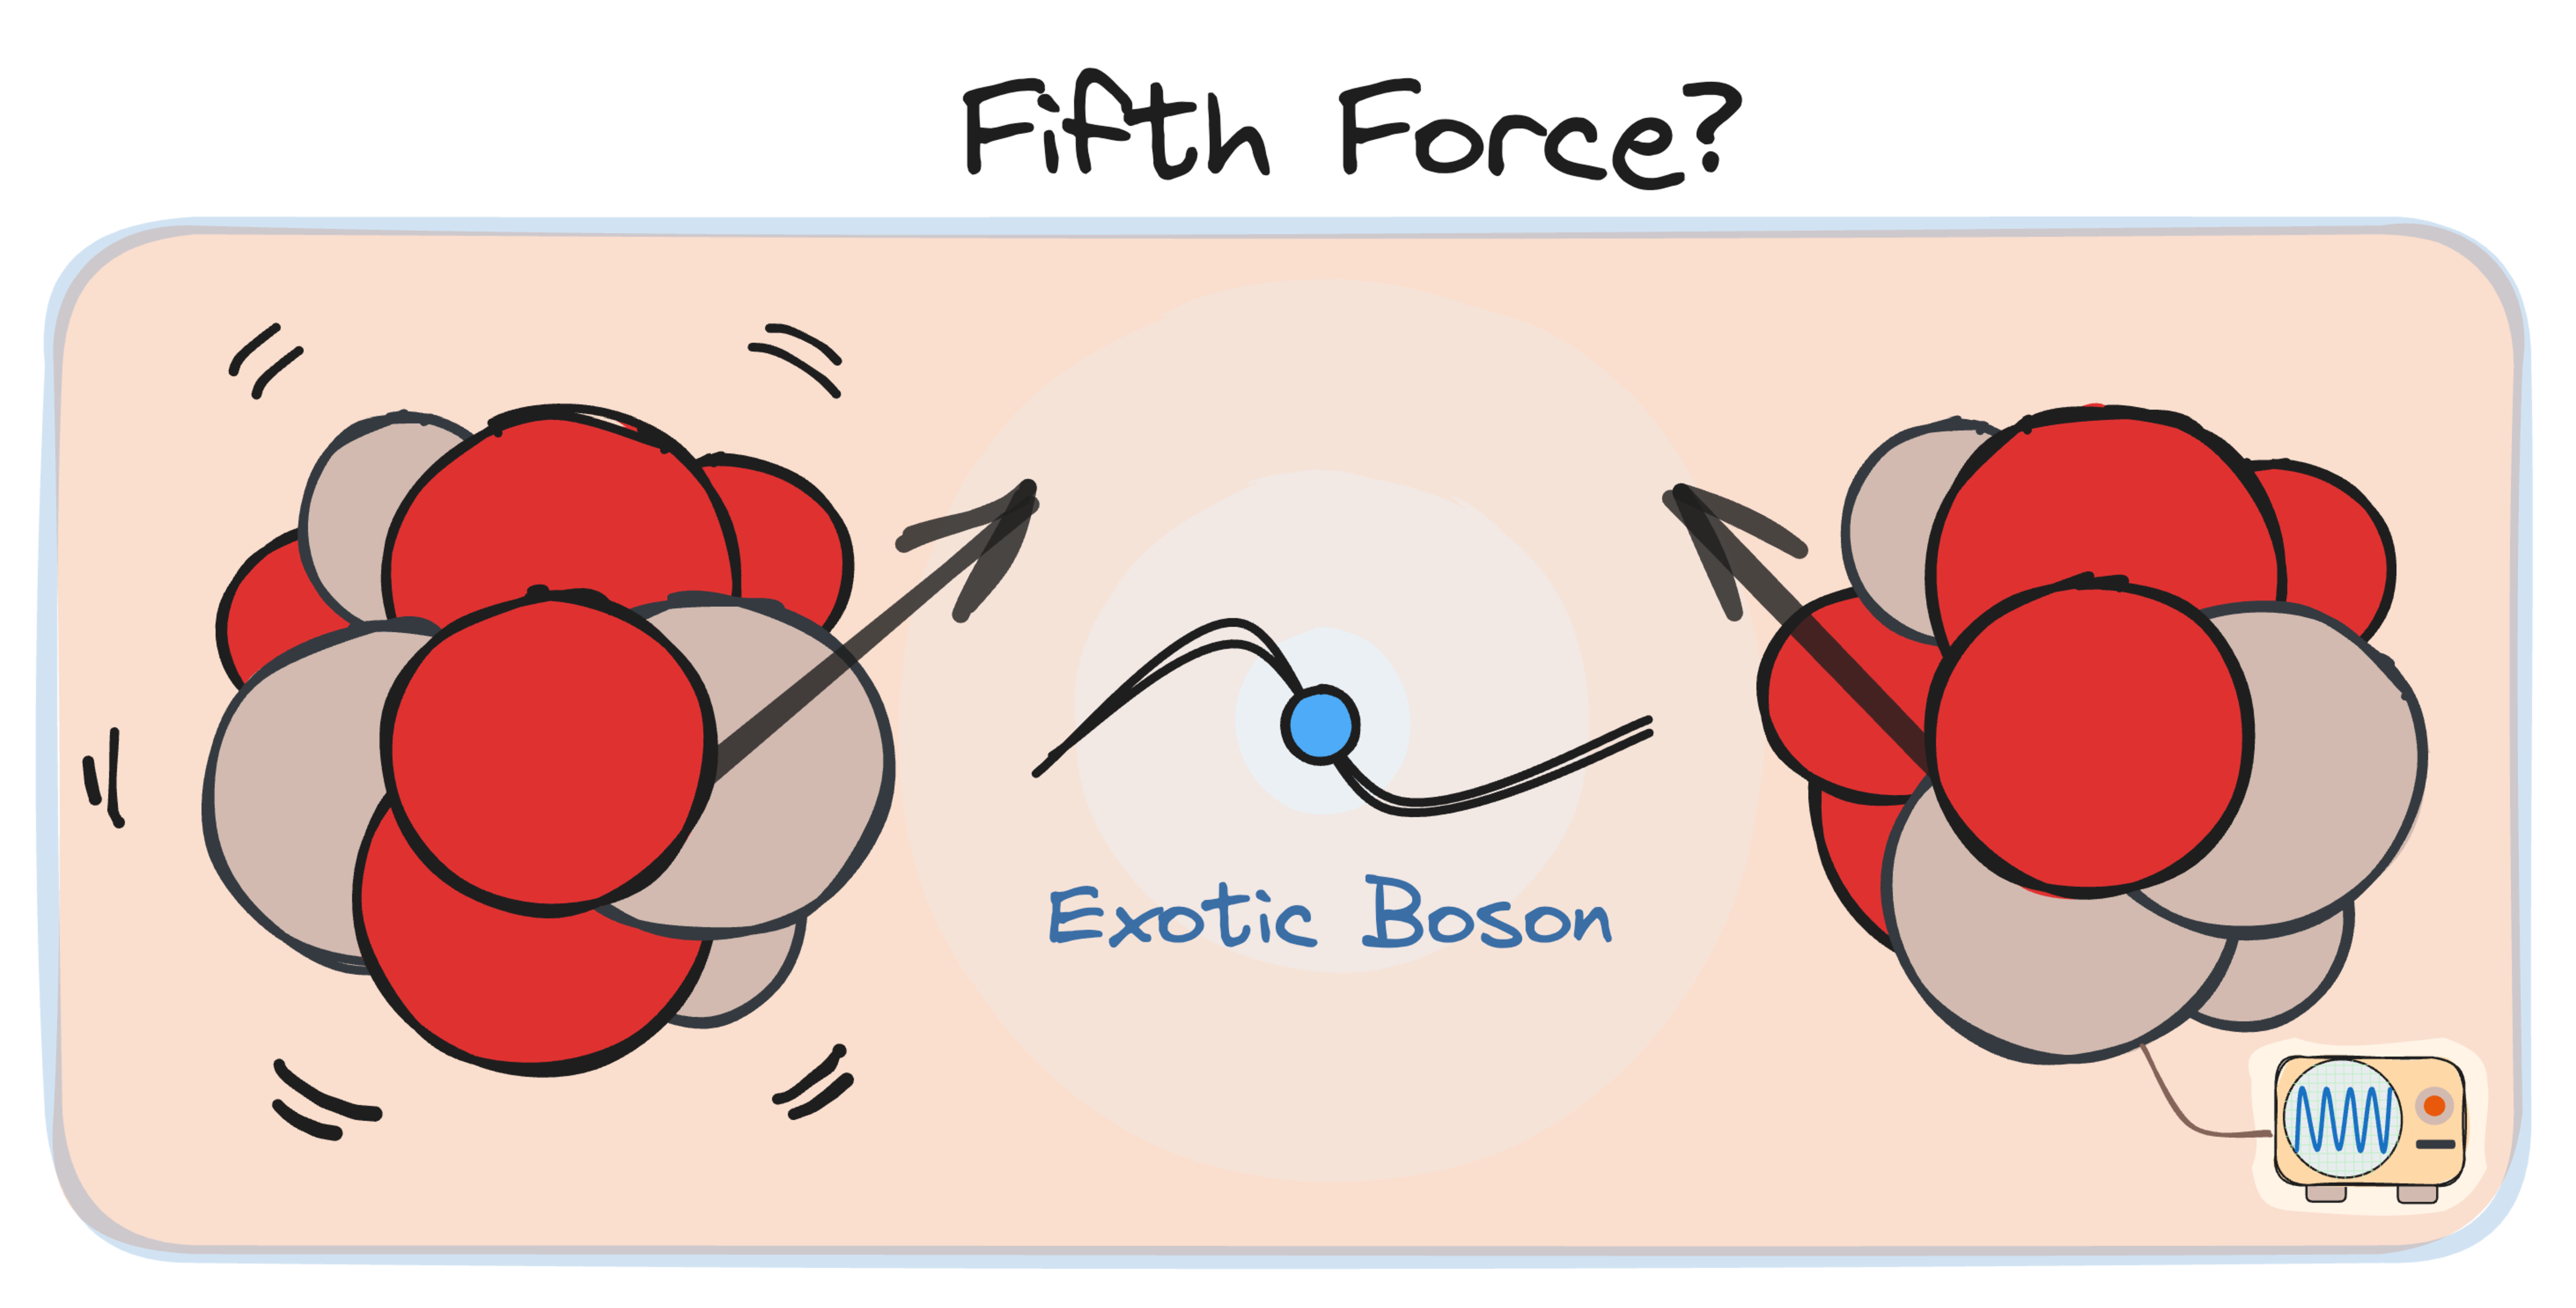
\includegraphics[width=0.45\textwidth]{Fig1.eps}
%\end{center}
\caption{(color online). 
An exotic boson carrying a fifth force that depends on the spins of the involved fermions.} 
\label{fifth-force}
\end{figure}

While there is currently no direct evidence for any fundamental interactions or forces beyond the established four,\footnote{Note that the discovery of the Higgs boson \cite{aad_observation_2012,chatrchyan_observation_2012}
indirectly suggests the presence of ``fifth force'' mediated by the exchange of Higgs bosons \cite{salam_higgs_2022}. Because of its relatively large mass ($\sim$125\,GeV/$c^2$) the Higgs-mediated force acts only over short distances, and has not yet been directly observed. 
However, the strength of this force is proportional to the product of the masses of the interacting fermions and this force gives a noticeable contribution to the energy of mesons containing heavy quarks; see, for example, \citet{flambaum_two_2011}.
%\citet{Two heavy fermions bound via Higgs boson exchange V.V. Flambaum, M. Yu. Kuchiev arXiv:1106.5220, Phys. Rev. D84, 114024  (2011)}.
} there is in principle no argument that would rule out such a possibility \cite{fayet_fifth_1986}. Instead, it is possible to constrain the strengths of such hypothetical forces using precise experimental measurements \cite{fischbach_reanalysis_1986,fischbach_six_1992}. 
% \DK{Saying ``until now'' implies that something happened now that makes it \underline{not} possible to constrain the strengths of such forces, which is not what we mean :).}
% If a fifth force were found to exist, it would be a groundbreaking discovery that would have significant implications for our understanding of the fundamental structure of the universe. 
% Fifth forces have been proposed as \DKIns{consequences arising from} possible explanations for \DKDel{deviations from the expected behavior of gravity and other fundamental forces}{ dark matter, dark energy, and baryogenesis, as well as from proposed solutions of the hierarchy problem and other mysteries of modern particle physics}. \DK{The problem with the formulation in terms of ``deivations from the expected behavior of gravity...'' is that no such deviations have been discovered and thus are not motivations for proposing fifth forces. Instead, the motivations for fifth forces are as consequences of theories aiming to solve other problems in physics.} These forces are thought to arise from the exchange of particles, and are predicted by some theories that go beyond the standard model.
Fifth forces are generally classified into two broad categories: those that depend on the spins of at least one of the interacting particles (spin-dependent forces) \cite{dobrescu_spin-dependent_2006,fadeev_revisiting_2019} and those that are independent of spins \cite{adelberger_tests_2003}. 
While both types of forces may arise within the same theoretical frameworks, in the current review we focus on spin-dependent forces, see Fig.\,\ref{fifth-force}.


%\LC{Victor and Derek suggest to make the background a little bit condensed.}
% If fifth forces do exist, they could have significant implications for our understanding of the universe and the fundamental forces that govern it. For example, as noted above, they could help to explain observed phenomena that are not fully accounted for by the standard model, such as the nature of dark matter and dark energy. Additionally, the study of these forces could provide new insights into the fundamental nature of the universe and help to advance our understanding of the fundamental forces.

\iffalse
\subsubsection{Spin and spin-dependent interactions }\label{Sec:Intro-bg-spin}


Spin is a fundamental property of elementary particles.  Spin-$1/2$ fermions can only possess two possible types of multipole moments: monopole moments (such as mass and charge) and dipole moments (such as  magnetic dipole moment, electric dipole moment and anapole moment). The Wigner-Eckart theorem \cite{sakurai_modern_2020} states that the dipole moment of a particle is proportional to its spin.
The idea of spin was inspired to explain the anomalous Zeeman effect, which is the result of the interaction of the magnetic dipole moment of an electron with an external magnetic field. For a history of the discovery of spin, see \citet{commins_electron_2012}. 

An example of a spin-dependent interaction is the magnetic dipole-dipole interaction between the magnetic moments of two particles \cite{griffiths_introduction_2018}. A manifestation of this interaction 
% \DKEdit{Another}{ An} example of \DKEdit{a spin-dependent}{ the effects of the magnetic dipole-dipole} interaction 
is the hyperfine structure (hfs) of atomic spectra, which arises from the interaction of the magnetic moments of the nucleus and electrons in an atom. 
% \DK{It seems like the example of the HF interaction is not different from a dipole-dipole interaction, and thus shouldn't be described as another example of an interaction distinct from the magnetic dipole-dipole case.} 
The hyperfine interaction causes splitting of atomic energy levels associated with different total angular momenta. 
% \DKDel{, and the size of the splitting can be influenced by the electric dipole moment of the atom.} \DK{I don't think the HF interaction has anything to do with the electric dipole moment of the atom (which is zero without CP-violation), and maybe for clarity it is easiest just to drop the second half of the sentence.}

Given the importance of spin in the interactions between particles, it is natural to ask what other spin-dependent interactions might exist between fermions apart from the magnetic dipole interaction \cite{safronova_search_2018}. %\DKDel{Studying these interactions could provide new information about the fundamental principles of the universe and could have important implications for the development of new technologies and theories.} \DK{I think the spirit of this last sentence was already captured earlier in the section, so it sounds a bit redundant. Maybe drop?}

%\subsubsection{Ultralight particles as dark matter (Derek)}\label{Sec:Intro-bg-DM}

%\DB{We need some content here!}

%\DK{Maybe this is not quite the correct section for this to appear in. I think it would make more sense in the next section on ``motivations.''}

%Ultra-light axion dark matter, \cite{abel_search_2023}. 

%Searching for Ultralight Scalar Dark Matter with Muonium and Muonic Atoms \cite{stadnik_searching_2023}. 

%The EPTA collaboration explored the possibility that pulsars can also act as ultra-light dark matter detectors. 
% \cite{european_pulsar_timing_array_second_2023}
\fi

\subsection{Motivation for searching for exotic spin-dependent interactions }\label{Sec:Intro-motiv}

%\DK{Perhaps the subsection titles should be somewhat rephrased to convey the ``motivation'' being communicated. The content can be more focused in this direction as well. I have attempted to do so below.}
%\LC{Ok}
The search for exotic spin-dependent interactions is motivated by a broad range of considerations spanning fundamental physics, astrophysics, and cosmology. From probing the properties of dark matter to understanding the quantum nature of gravity, spin-dependent forces provide a unique avenue for exploring physics beyond the SM. Such interactions, often mediated by hypothetical particles like axions, axionlike particles, or other exotic bosons, have the potential to address profound mysteries, including the strong CP problem, the nature of dark energy, and the matter-antimatter asymmetry of the universe. The following sections outline the theoretical underpinnings and experimental efforts that establish this field as a vibrant frontier of modern physics.

\subsubsection{Role of intrinsic spin in gravity}\label{Sec:Intro-motiv-spin-gravity}

The idea of intrinsic spin, which is a particular kind of angular momentum, comes from relativistic quantum mechanics or quantum field theory. 
However, in contrast to orbital angular momentum, it cannot be understood as arising from the physical rotation of an object. 
In the early days of the development of quantum mechanics, 
%\YS{
soon after the discovery of the Pauli spin matrix formalism,
%} 
researchers tried to understand how to incorporate the concept of spin into the framework of general relativity, which describes the force of gravity, attempting to extend our understanding of gravity to the quantum level.

One way to incorporate spin into general relativity is through the concept of spacetime torsion \cite{de_sabbata_spin_1994}.
Torsion quantifies the twisting of a coordinate system as it is transported along a curve. 
In Einsteinian general relativity, mass (energy) generates curvature of spacetime, but the torsion is zero. 
However, in an extension of general relativity proposed by \citet{cartan_generalization_1922}, torsion is introduced as an additional aspect of spacetime: torsion is caused by the spin of particles and can also influence particle dynamics
\cite{hehl_general_1976}. 
This extension, known as Einstein-Cartan theory, is still a subject of ongoing research.

% \DKDel{In general relativity, the curvature of space-time is caused by the presence of matter and energy, and this curvature dictates the motion of objects. Torsion gravity proposes that there is an additional aspect of space-time, known as torsion, which is caused by the spin of particles and can also influence the motion of objects.} \DK{As this was redundant with above discussion, I tried to merge and simplify.}

%\DKDel{Initially, a principal} 
Consequently, one theoretical impetus encouraging experimental searches for exotic spin-dependent interactions is speculation concerning the possibility of a torsion-related spin-gravity coupling manifesting as a gravitational dipole moment (GDM) of elementary fermions (\citealp{morgan_direct_1962}; \citealp{kobzarev_gravitational_1963}; \citealp{leitner_parity_1964}; \citealp{dass_test_1976}; \citealp{peres_test_1978}), or a gravitomagnetic force \cite{mashhoon_gravitomagnetic_2021}. 
%\YS{missing reference} \DK{Perhaps a good reference here could be: B. Mashhoon, ``Gravitomagnetic Stern-Gerlach Force,'' Entropy \textbf{23}, 445 (2021).} or a torsion field \cite{neville_experimental_1980}. 
If a spin-gravity coupling exists, then particles with a nonzero GDM would experience a spin-dependent force in the presence of a gravitational field.

% \DKDel{Another way in which spin-gravity coupling could manifest is through a spin-dependent gravitational interaction known as the gravitomagnetic force. This force is analogous to the magnetic force experienced by moving charged particles in an electromagnetic field. In the case of the gravitomagnetic force, the spinning particles would experience a force due to their motion relative to the gravitational field.}

Gravitomagnetism is a particularly interesting case to consider, as it provides a clear testable example of the most straightforward way to extend general relativity to incorporate intrinsic spin (\citealp{silenko_semiclassical_2005}; \citealp{adler_gravitomagnetism_2012}; \citealp{mashhoon_spin_2013}).
%[references: B. Mashhoon and Y. N. Obukhov, ``Spin precession in inertial and gravitational fields,'' Phys. Rev. D \textbf{88}, 064037 (2013); R. J. Adler, P. Chen, and E. Varani, ``Gravitomagnetism and spinor quantum mechanics,'' Phys. Rev. D \textbf{85}, 025016 (2012); A. J. Silenko and O. V. Teryaev, ``Semiclassical limit for Dirac particles interacting with a gravitational field,'' Phys. Rev. D {\textbf{71}}, 064016 (2005).]. 
General relativity predicts that massive bodies drag spacetime around with them as they rotate, which consequently leads to precession of macroscopic gyroscopes. This is the Lense-Thirring effect \cite{lense_uber_1918} 
%[reference: J. Lense and H. Thirring, \"Uber die einfluss der eigenrotation der zentralk\"orper auf die bewegung der planeten und monde nach der Einsteinschen gravitationstheorie,'' Phys. Z. {\textbf{19}}, 156 (1918)] 
measured, for example, by the Gravity Probe B mission \cite{everitt_gravity_2011}. %[reference: C.W. F. Everitt et al., ``Gravity Probe B: Final Results of a Space Experiment to Test General Relativity,'' Phys. Rev. Lett. \textbf{106}, 221101 (2011)]. 
It remains an experimentally open question as to whether intrinsic spins undergo general relativistic precession as do macroscopic rotating objects, and there have been recent proposals to develop experimental probes to answer this question \cite{fadeev_gravity_2021}.\footnote{Note also the related work of \citet{trukhanova_search_2023}, who investigated the effects of torsion on the electromagnetic field, specifically the ``electric'' and ``magnetic'' components of the torsion field. 
They derived modified Maxwell's equations that describe how the electromagnetic field behaves in the presence of torsion, and studied propagation of electromagnetic waves under the influence of a uniform, homogeneous torsion field. 
They showed that in the presence of a nonzero torsion field, such a wave exhibits a Faraday effect, in which the polarization of the wave is rotated, and used astrophysical data to set a bound on the possible coupling/interaction strength of cosmic axial torsion fields.} %[reference: P. Fadeev et al., ``Gravity Probe Spin: Prospects for measuring general-relativistic precession of intrinsic spin using a ferromagnetic gyroscope,'' Phys. Rev. D \textbf{103}, 044056 (2021)].}
% \DKDel{In addition, another way in which a spin-gravity coupling could manifest is through a hypothetical field known as a torsion field.} \DK{Seems redundant.} 
% \YS{Do they (need to) assume this as an additional assumption or does the Faraday effect simply arise as a consequence of the torsion field? If so, then should clarify the wording here accordingly.} \DK{I agree with Yevgeny's point and edited the above sentence accordingly.}
% \DB{Dear Colleagues, I would like to put a word of caution here regarding a possible confusion between spin-gravity and include something along the lines of:}
% \DB{We note that an effect that mimics GDM may arise from exotic beyond-the-standard-model fields sourced by the Earth, in which case the `GDM' terminology would be a misnomer and one should rather talk about an exotic `monopole--dipole' coupling (having nothing to do with gravity), where monopole refers to the Earth and dipole refers to the spin. }
% \DK{I wholeheartedly agree with Dima. I have inserted some suggested text below. Overall, this section I.B.1 looks great to me, nice work!}

When considering the possibility of the existence of gravitational torsion and how it could be detected using spin-based sensors, a subtle issue arises. Namely, how does one differentiate torsion from new spin-dependent forces that are mediated by exotic bosons that have no particular connection to gravity? 

On the one hand, effects that manifest at a level consistent with the strength of the gravitational force and with universal coupling proportional to mass would suggest a connection. Another characteristic that would strongly hint that a newly found spin-dependent interaction was connected to torsion would be if it satisfied the equivalence principle. This would mean that accelerating frames would be indistinguishable from gravitational fields in terms of the spin-precession effects they induce \cite{singh_einstein_1997}.
%\DK{Cite: P. Singh and L. H. Ryder, ``Einstein - Cartan - Dirac theory in the low-energy limit'' Class. Quantum Grav. 14 3513 (1997)}.  
%\YS{Look good.}
On the other hand, in many models of torsion where the coupling strength is a free parameter, the distinction may be purely semantic. An example of this is the appearance of torsion in scalar-vector-tensor extensions of general relativity \cite{heisenberg_systematic_2019,aoki_ghostfree_2019}. Therefore, measurement of a coupling between spins and mass could be equally well described by particular models of gravitational torsion as well as an exotic spin-0 field with both scalar and pseudoscalar interactions which would generate a monopole-dipole coupling. Another possible source of monopole-dipole interactions is an exotic spin-1 boson \cite{fayet_new_1996}; see Fig.\,\ref{New-bosons} and Sec.\,\ref{Subsec:Fformalism} and \ref{Subsec:Pairs-pots.} for details.


%\DB{This is a very nice subsection. But please explain, why the discussion of possible experiments in a centrifuge has been cut out?} \DK{Added a couple sentences in the middle of the above paragraph, hopefully good now! Also found a useful reference!} \LC{Dear Derek, many thanks!}

% cut from here 
%\subsubsection{Atomic parity violation}\label{Sec:Intro-motiv-APV}


%\subsubsection{Electric dipole moment}\label{Sec:Intro-motiv-EDM}


\subsubsection{Ultralight bosons as dark matter}\label{Sec:Intro-motiv-DM}

%\DK{I propose to move this ultralight dark matter section here as opposed to above.}\LC{OK}

Cosmological and astrophysical observations indicate that the majority of matter is invisible and non-luminous ``dark matter'' -- estimated to constitute over 80\% of the matter mass fraction in the Universe (\citealp{spergel_dark_2015}; \citealp{bertone_new_2018}).
%\DK{Cite: [D. N. Spergel, Science {\textbf{347}}, 1100 (2015).] and [G. Bertone and T. M. P. Tait, Nature (London) {\textbf{562}}, 51 (2018).] }. 
To understand the microscopic nature of this dark matter is a major objective of cosmology, astrophysics and particle physics, as it could provide insight into the early Universe and uncover new physical laws (\citealp{bertone_particle_2005}; \citealp{feng_dark_2010}; \citealp{chadha-day_axion_2022}). %\cite{bertone_particle_2005,feng_dark_2010,chadha-day_axion_2022}. 
%\DK{Cite: [Gianfranco Bertone, Dan Hooper, and Joseph Silk, ``Particle dark matter: Evidence, candidates and constraints.'' Physics reports {\textbf{405}}, 279 (2005).], [Jonathan L. Feng, ``Dark matter candidates from particle physics and methods of detection.'' Annual Review of Astronomy and Astrophysics {\textbf{48}}, 495 (2010).], and [Francesca Chadha-Day, John Ellis, and David J.E. Marsh. ``Axion dark matter: What is it and why now?'' Science advances {\textbf{8}}, eabj3618 (2022).]}. 
The evidence for the existence of dark matter is based entirely on its gravitational effects, which can be observed on a galactic scale and beyond, such as in measurements of galactic rotation curves \cite{rubin_rotation_1970},
%\DK{Cite: [V.C. Rubin, W.K. Ford Jr, Astrophys. J. {\textbf{159}}, 379 (1970).]}
observations of the velocity dispersion of galactic clusters \cite{zwicky_masses_1937}
%\DK{Cite: [F. Zwicky, Astrophys. J. \textbf{86}, 217 (1937).]} 
and colliding galactic clusters \cite{clowe_direct_2006},
%\DK{Cite: [D. Clowe, M. Bradac, A.H. Gonzalez, M. Markevitch, S.W. Randall, C. Jones, D. Zaritsky, Astrophys. J. Lett. {\textbf{648}}, L109 (2006).]}
the formation of large-scale structure in the Universe (\citealp{springel_simulations_2005}; \citealp{angulo_large-scale_2022}),
%\cite{angulo_large-scale_2022,springel_simulations_2005},
%\DK{Cite: [Raul E. Angulo and Oliver Hahn, ``Large-scale dark matter simulations.'' Living Reviews in Computational Astrophysics {\textbf{8}}, 1 (2022).] and [Volker Springel et al., ``Simulations of the formation, evolution and clustering of galaxies and quasars." Nature {\textbf{435}}, 629 (2005).]}
and studies of the cosmic microwave background radiation \cite{bennett_nine-year_2013,planck_collaboration_planck_2016,hinshaw_nine-year_2013}.
%\DK{Cite: [C.L. Bennett, D. Larson, J. Weiland, N. Jarosik, G. Hinshaw, N. Odegard, K. Smith, R. Hill, B. Gold, M. Halpern et al., Astrophys. J. Suppl. 208, 20 (2013).], [P.A. Ade, N. Aghanim, M. Arnaud, M. Ashdown, J. Aumont, C. Baccigalupi, A. Banday, R. Barreiro, J. Bartlett, N. Bartolo et al., Astron. Astrophys. 594, A13 (2016).], and [G. Hinshaw, D. Larson, E. Komatsu, D.N. Spergel, C. Bennett, J. Dunkley, M. Nolta, M. Halpern, R. Hill, N. Odegard et al., Astrophys. J. Suppl. 208, 19 (2013).]}. 
Ultimately, to understand the microscopic nature of dark matter, it is crucial to try to measure its non-gravitational interactions with particles and fields of the SM. 

A potential explanation for dark matter is that it consists of ultralight bosons, with masses less than about one eV.
If such bosons indeed exist, they could interact with spins and thus mediate spin-dependent interactions as described in the present review.
The hypothesis that dark matter is made of ultralight bosons is among the most compelling motivations to search for new spin-dependent interactions, as discussed, for example, by \citet{jackson_kimball_search_2023}.

Like the vast majority of galaxies observed to date, it is believed that the stars of the Milky Way are embedded within and rotate through a spherical dark matter halo (\citealp{navarro_structure_1996-1}; \citealp{jiao_detection_2023}).
%\cite{navarro_structure_1996-1,jiao_detection_2023}.
%\DK{Cite: [Julio F. Navarro, ``The structure of cold dark matter halos.'' Symposium-international astronomical union. Vol. 171. Cambridge University Press, 1996.], [M. Kamionkowski and S.M. Koushiappas, Phys. Rev. D {\textbf{77}}, 103509 (2008).], and [Yongjun Jiao et al., ``Detection of the Keplerian decline in the Milky Way rotation curve.'' Astronomy \& Astrophysics {\textbf{678}}, A208 (2023).]}.
In addition to searching for new forces mediated by such ultralight bosons, if the ultralight bosons constitute the dark matter, one can attempt to directly detect the interaction of the bosonic dark matter with quantum sensors.
This is the strategy of ``haloscope'' experiments such as the long-running Axion Dark Matter eXperiment, ADMX 
\cite{admx_collaboration_search_2018,admx_collaboration_extended_2020}.
%\DB{Please remove the ``et al." here. There is some option in the cite command for this.} %\LC{I have tried \collabcite{admx_collaboration_search_2018}, and \citeauthor*{admx_collaboration_search_2018} (\citeyear{admx_collaboration_search_2018}), didn't work.}
%\YS{One possible brute-force way to remove the ``et al.'' here could be to manually remove the author names from the ``author'' field in the MyLibrary.bib file and keep only ``ADMX Collaboration'' in this field. We can leave the author list commented out in the MyLibrary.bib file for the editors in case they need this.}\LCa{That is a good suggestion. We will try to do this soon.}
%\DK{Cite: [Nick Du et al., ``Search for invisible axion dark matter with the axion dark matter experiment.'' Physical Review Letters {\textbf{120}}, 151301 (2018).] and [Thomas Braine et al., ``Extended search for the invisible axion with the axion dark matter experiment.'' Physical review letters {\textbf{124}}, 101303 (2020).]}.

Thanks to the progress made in superconducting microwave cavities, magnetic resonance techniques, atomic interferometry, magnetometry, and atomic clocks, a range of experimental ideas have been proposed to use quantum sensors based on these technologies to look for bosonic dark matter candidates with masses between $10^{-22}$ and $10^{-3}$ eV (\citealp{semertzidis_axion_2022}; \citealp{adams_axion_2022}; \citealp{antypas_new_2022}; \citealp{fedderke_measuring_2024}).
%\DK{Cite: [Yannis K. Semertzidis and Sung Woo Youn, ``Axion dark matter: How to see it?'' Science Advances {\textbf{8}}, eabm9928 (2022).], [C. B. Adams et al., ``Axion dark matter.'' arXiv:2203.14923 (2022).], and [D. Antypas et al., ``New horizons: scalar and vector ultralight dark matter.'' arXiv:2203.14915 (2022).]}. 
Additionally, ways to investigate ultra-heavy, composite dark matter objects with both astrophysical and terrestrial measurements have been developed (\citealp{pustelny_global_2013}; \citealp{derevianko_hunting_2014}; \citealp{roberts_search_2017}; \citealp{afach_search_2021,afach_what_2023}). %\cite{pustelny_global_2013,derevianko_hunting_2014,roberts_search_2017,afach_search_2021,afach_what_2023}.
%\DK{Cite: [Szymon Pustelny et al., ``The Global Network of Optical Magnetometers for Exotic physics (GNOME): A novel scheme to search for physics beyond the Standard Model.'' Annalen der Physik {\textbf{525}}, 659 (2013).], 
%[A. Derevianko and M. Pospelov, Nat. Phys. {\textbf{10}}, 933 (2014).], 
%[B.M. Roberts, G. Blewitt, C. Dailey, M. Murphy, M. Pospelov, A. Rollings, J. Sherman, W. Williams, A. Derevianko, Nat. Comm. {\textbf{8}}, 1195 (2017).],
%[Samer Afach et al., ``Search for topological defect dark matter with a global network of optical magnetometers.'' Nature Physics {\textbf{17}}, 1396 (2021).], 
%and [Samer Afach et al., ``What Can a GNOME Do? Search Targets for the Global Network of Optical Magnetometers for Exotic Physics Searches.'' Annalen der Physik 2023, 2300083 (2023).]}.
Such dark matter haloscope experiments and their connections to searches for boson-mediated spin-dependent interactions that are the focus of this review are briefly summarized in Sec.\,\ref{METH2.DM}. 
% \DB{I suggested adding the following to explain the motivation explicitly: 
The ``dark matter connection'' provides a strong motivation to search for exotic spin-dependent interactions. %}

%\DB{I suggest using \, instead of ~ to make a small unbreakable gap.}

%\subsubsection{The strong-$CP$ problem}\label{Sec:Intro-motiv-spin-0}
\subsubsection{The strong-\texorpdfstring{$CP$}{CP} problem}\label{Sec:Intro-motiv-spin-0}

% \LC{I made a new version below and absorbed some comments from the original version, but may still need to check and improve. }
% [

One of the first and most influential proposals for an exotic boson that couples to spin was the axion (\citealp{weinberg_new_1978}; \citealp{wilczek_problem_1978}; \citealp{kim_weak-interaction_1979}; \citealp{zhitnitsky_possible_1980}; \citealp{shifman_can_1980}; \citealp{dine_simple_1981}).
%\cite{dine_simple_1981,zhitnitsky_possible_1980, kim_weak-interaction_1979, shifman_can_1980, weinberg_new_1978, wilczek_problem_1978}.
The axion is a consequence of a proposed solution to the strong-$CP$ problem in quantum chromodynamics (QCD) \cite{peccei_constraints_1977, peccei_mathrmcp_1977}, where $CP$ is the combined charge-conjugation ($C$) and parity ($P$) symmetry. 
The strong-$CP$ problem, reviewed by \citet{peccei_strong_2008}, is a so-called ``fine-tuning'' problem of why the observable $CP$-violating phase in the QCD Lagrangian, $\theta_{\rm{QCD}}$, is extremely small, %\DB{
presently constrained to be smaller than $10^{-10}\,$rad, 
%}
as determined through measurements of 
%\DB{One cannot use ``e.g.'' here; I can explain the rule, if you like} 
the $CP$-violating permanent electric dipole moment (EDM) of the neutron \cite{abel_measurement_2020} and the EDM of the mercury atom \cite{graner_reduced_2016}.
%\DK{Cite: [C. Abel et al. (nEDM Collaboration), ``Measurement of the Permanent Electric Dipole Moment of the Neutron.'' Phys. Rev. Lett. {\textbf{124}}, 081803 (2020).]}, 
Naively, one would expect $\theta_{\rm{QCD}}$ to be much larger, namely $\mathcal{O}(1)$. 
Notably, axions are also a leading dark matter candidate \cite{preskill_cosmology_1983,abbott_cosmological_1983,dine_not-so-harmless_1983}, see also \citet{jackson_kimball_search_2023}.  
%\DB{I separated the book from the original work; it looked a bit funny otherwise}
% (more precisely) of order one, $\mathcal{O}(1)$. 

To solve the strong-$CP$ problem, \citet{peccei_constraints_1977,peccei_mathrmcp_1977} proposed introducing a new global chiral $U(1)$ symmetry, subsequently referred to as the Peccei-Quinn (PQ) symmetry. In this scenario, the $CP$-violating phase $\theta_{\rm{QCD}}$ is not a constant but instead evolves dynamically and tends to a value close to zero due to the spontaneous breaking of the PQ symmetry \cite{weinberg_new_1978,wilczek_problem_1978}. 
%\YS{I'm not sure that Peccei and Quinn were the first to postulate a dynamical axion field in 1977. I think this was done by Weinberg and Wilczek (separately) in 1978 by building on Peccei-Quinn's earlier 1977 papers about the U(1) PQ symmetry. Please check.} 
In this model, the $CP$-violating phase in the QCD Lagrangian is coupled to the dynamical axion field $a$ such that $\theta_{\rm{QCD}} \rightarrow \theta_{\text{eff}} = \theta_{\rm{QCD}} + {a}/{f_a}$, where $f_a$ is the axion decay constant ($f_a$ is proportional to the energy scale of the PQ symmetry breaking). The quantum of this field is a spin-0 particle known as the axion. Due to instanton\footnote{Instantons refer to classical solutions of the QCD field equations with nontrivial topologies.} effects \cite{vainshtein_abc_1982,coleman_uses_1979}, 
%\YS{Is it possible to have the "i"'s in the Vainshtein reference appear with the usual single dot instead of inverted circumflexes?}\LCa{Done.}
%\DK{Cite: [A. I. Vainshtein et al. ``ABC of instantons.'' Soviet Physics Uspekhi {\textbf{25}}, 195 (1982).] and [Sidney Coleman, ``The uses of instantons.'' in The whys of subnuclear physics, pp. 805-941 (Springer, Boston, 1979).]}, 
the axion field acquires an effective potential of the form $V_\textrm{eff} \propto - \cos(\theta_\textrm{eff})$, for which the energy (as well as the amount of $CP$ violation) is minimized at $\theta_\textrm{eff} = 0$.\footnote{Initially, the axion model was called the Peccei-Quinn-Weinberg-Wilczek (PQWW) model \cite{peccei_constraints_1977,peccei_mathrmcp_1977,weinberg_new_1978,wilczek_problem_1978}. However, this model predicted unobserved consequences for existing particle properties, so it was quickly ruled out by experiments. Subsequently, it was proposed to increase the energy scale of the PQ symmetry breaking in the model characterized by a larger $f_a$. 
This made the axion much lighter and is the essence of the Dine-Fischler-Srednicki-Zhitnitsky (DFSZ) axion model 
(\citealp{zhitnitsky_possible_1980}; \citealp{dine_simple_1981}),
%\cite{zhitnitsky_possible_1980,dine_simple_1981}, 
a so-called ``invisible axion'' model. 
Another invisible axion model is the Kim-Shifman-Vainshtein-Zakharov (KSVZ) model (\citealp{kim_weak-interaction_1979}; \citealp{shifman_can_1980}). 
%\cite{kim_weak-interaction_1979,shifman_can_1980}. 
Note that the KSVZ model assumes that the axion couples at tree level only to a super-heavy, as yet unobserved, quark, while the SM fermions do not couple to the axion at tree level.}

The axion typically couples to the axial-vector current of fermions through a derivative interaction of the form $ \partial_{\mu} \left( {a}/{f_a} \right) \bar{\Psi} \gamma^{\mu} \gamma^5 \Psi $, where $ \bar{\Psi} $ is the Dirac adjoint of the fermion field $\Psi$. 
This coupling to the axial-vector current indicates that the axion momentum interacts with the spin of the fermion. 
On macroscopic scales, the axion field can be interpreted as mediating monopole-dipole and dipole-dipole interactions as discussed by \citet{moody_new_1984}; note also early work by \citet{anselm_possible_1982} discussing a long-range dipole-dipole interaction mediated by ``arions'' -- particles closely related to axions. 
\citet{moody_new_1984} noted that a spin-0 field $\phi$ can couple to fermions in two ways: through a scalar vertex or through a pseudoscalar vertex. 
In the nonrelativistic limit, a fermion coupling to a scalar vertex behaves like a monopole at leading order, while a fermion coupling to a pseudoscalar vertex behaves like a dipole. 
This is related to the fact that in the center-of-mass (C.M.) frame of the particles, there are only two vectors that can be used to form a scalar or pseudoscalar quantity: spin and momentum. 
If the vertex does not involve the fermion spin at leading order in the nonrelativistic approximation, it is a monopole coupling, but if it does involve the spin, it depends on the dot (scalar) product of the spin and momentum, which is a $P$-odd (parity-odd) pseudoscalar term. 
Therefore, it is the pseudoscalar coupling of particles such as axions or axionlike particles that is responsible for generating new dipole interactions. 
%\MK{Note that abbreviation ALPs is introduced only in the next section!}
%\YS{Indeed. I think it's better to use the full term for ALPs above (now updated).}\LCa{Thanks. I will check this problem throughout the manuscuript soon.}

The insights of \citet{moody_new_1984} sparked considerable interest in the search for exotic spin-dependent interactions; see, for example, discussions of theoretical developments in Sec.\,\ref{Sec:formalism} and experimental research in Secs.\,\ref{subsec_g_Pg_S} and \ref{subsec_g_Pg_P}.


\subsubsection{Quantum theories of gravity and axionlike particles (ALPs)}
\label{Sec:Intro-motiv-quantum-gravity}

%\DB{I had a though that it could be more logical to put this subsection second to have the subsections related to gravity together. However, this section talks about ALPs also. So I just modified the title of the subsection; it can stay here}
Physicists have long sought to develop a unified theory of the four fundamental forces of nature: gravity, electromagnetism, the weak force, and the strong force. 
The aim of such a unified theory is to create a single theoretical framework that can explain all interactions in the universe. 
However, combining gravity with the other forces, which are described by quantum field theory in the SM, has thus far been unsuccessful due to the fact that the theory of general relativity breaks down at small distances (high energies).

String theory is a leading hypothesis for unifying gravity with the SM of particle physics (\citealp{zwiebach_first_2004}; \citealp{green_superstring_2012-1,green_superstring_2012}).
%\cite{green_superstring_2012-1,green_superstring_2012,zwiebach_first_2004}.
%\DK{Cite: [Michael B. Green, John H. Schwarz, and Edward Witten. ``Superstring theory: volume 1 introduction.'' (Cambridge university press, 2012).], [Michael B. Green, John H. Schwarz, and Edward Witten. ``Superstring theory: volume 2 loop amplitudes, anomalies and phenomenology.'' (Cambridge university press, 2012).], and [Barton Zwiebach, ``A first course in string theory.'' (Cambridge University Press, 2004).]}. 
It proposes that the matter in the universe is composed of ``strings'' that vibrate in additional dimensions with very small (compared to everyday) 
%\DB{Neither ``very'' nor ``small'' is allowed in a physics text without making it clear what the comparison scale is. What are the length scales for strings?}
length scales. 
%The familiar characteristics of particles and fields are thought to arise from the twisting, folding, and oscillation of these fundamental strings. \DB{This last sentence looks like a product of AI and, while very nice, cane be deleted as it does not add much to the information in the previous sentence.}

%Axion-like \DB{Have not we decided to write this as one word: axionlike?} 
Axionlike particles (ALPs), spin-0 bosons with properties similar to those of axions \cite{jaeckel_low-energy_2010}, have been suggested to exist in string theory as excitations of quantum fields that extend into the additional spacetime dimensions beyond the four we are familiar with \cite{bailin_kaluza-klein_1987,svrcek_axions_2006}. 
%\DK{Cite: [P. Svrcek and E. Witten, ``Axions in string theory,'' J. High Energy Phys. {\textbf{06}}, 051 (2006).]}. 
%Arvanitaki et al. (2010) 
\citet{arvanitaki_string_2010}
%\DK{Cite: [A. Arvanitaki, S. Dimopoulos, S. Dubovsky, N. Kaloper, and J. March-Russell, ``String axiverse,'' Phys. Rev. D {\textbf{81}}, 123530 (2010).]} 
proposed that, due to the complexity of the extra-dimensional manifolds of string theory, there should be many ultralight ALPs, possibly spanning each decade of mass down to the present-day Hubble scale of $10^{-33}$~eV, referred to as an ``axiverse.''

An important feature of ALPs, not only those from string theory but those arising generically in beyond-SM physics scenarios, is that the relationship between the ALP mass and the ALP decay constant $f_a$, and subsequently the ALP's interaction strength with SM particles and fields, is not as strongly constrained by theory as in the case of QCD axions \cite{marsh_axions_2017}. 
%\DK{Cite: [David J.E. Marsh, ``Axions and ALPs: a very short introduction.'' arXiv:1712.03018 (2017).]}. 
This opens a broader theoretically motivated parameter space to search for evidence of exotic spin-dependent interactions.



\subsubsection{The matter-antimatter asymmetry of the universe}
\label{Sec:Intro-motiv-matter-antimatter}

One of the most important problems in theoretical physics is to identify the cause of the matter-antimatter asymmetry of the Universe 
(\citealp{dine_origin_2003}; \citealp{canetti_matter_2012}).
%\cite{dine_origin_2003,canetti_matter_2012}.
%\DK{Cite: [Michael Dine and Alexander Kusenko, ``Origin of the matter-antimatter asymmetry.'' Rev. Mod. Phys. {\textbf{76}}, 1 (2003).]} 
There is strong evidence that there are no large concentrations of antimatter at any scale in the present universe
%other than cosmic %\DB{What does ``cosmic'' mean? Is galactic scale a cosmic scale? The sentence also seems to imply that there is concentration %of antimatter at a cosmic scale. I do not think there is...} 
\cite{cohen_matter-antimatter_1998}.
%\DK{Cite: [Andrew G. Cohen, Alvaro De R\'ujula, and Sheldon Lee Glashow, ``A matter-antimatter universe?'' The Astrophysical Journal {\textbf{495}}, 539 (1998).]}. 
%Sakharov \DK{Cite: [A. D. Sakharov, JETP Lett. {\textbf{6}}, 24 (1967).]} 
\citet{sakharov_violation_1967} 
%\LC{Dear Derek, could you please double check the reference we cite here: [A. D. Sakharov, JETP Lett. {\textbf{6}}, 24 (1967).]. Could it be: Sakharov, A. D., 1967, “Violation of CP invariance, C asymmetry, and baryon asymmetry of the universe,” ZhETF Pis’ma 5, 32 [JETP Lett. 5, 24 (1967)].} \DK{Dear Lei, I think you are correct that the reference you note is the one I intended to cite, so that would be good to update properly. Nice catch!} \LC{Dear Derek, thank you! i have updated it.} 
proposed that the baryon density may not be a result of some initial condition, but could in fact be explained by particle physics interactions in the early universe. Theory suggests that in order to generate the observed baryon density in the universe (and the lack of anti-baryons), some baryon-number- and lepton-number-violating interactions and, particularly, new sources of $CP$-violation are necessary \cite{shaposhnikov_baryon_1987}.
%\DK{Cite: [M. E. Shaposhnikov, ``Baryon asymmetry of the universe in standard electroweak theory.'' Nuclear Physics B {\textbf{287}}, 757 (1987).]}.
The presence of exotic bosons could potentially provide a solution to this problem of baryogenesis.

A theoretical model to explain baryogenesis using axions was developed by \citet{co_axiogenesis_2020}, and a closely related ALP-based theory of baryogenesis was discussed by \citet{co_lepto-axiogenesis_2021} and \citet{co_predictions_2021}.
%\DK{Cite: [R. T. Co, N. Fernandez, A. Ghalsasi, L. J. Hall, and K. Harigaya, ``Lepto-axiogenesis.'' JHEP {\textbf{3}} (arXiv: 2006.05687), 017 (2021).]} and \DK{Cite: [Raymond T. Co, Lawrence J. Hall, and Keisuke Harigaya, ``Predictions for axion couplings from ALP cogenesis.'' Journal of High Energy Physics {\textbf{2021}}, 172 (2021).]}. 
In these axiogenesis and ALP-cogenesis models, explicit symmetry breaking in the early universe leads to a time-dependent $\theta_{\text{eff}}$ (i.e., $d\theta_{\text{eff}}/dt \neq 0$, implying a ``rotation'' of the axion or ALP fields). A nonzero $d\theta_{\text{eff}}/dt$ at the weak scale satisfies the out-of-equilibrium and $CP$-violation conditions for baryogenesis, and creates the baryon-antibaryon asymmetry via QCD and electroweak effects in the case of axions, or via couplings with photons, nucleons, and/or electrons in the ALP case.
%\DB{
This motivates searches for axions and ALPs, including probing their existence through spin-dependent forces discussed here.%}

\subsubsection{The hierarchy problem}
\label{Sec:Intro-motiv-hierarchy-problem}

One of the most perplexing issues in theoretical physics is the hierarchy problem: why is gravity so much weaker than the other forces? The core of this conundrum is why the observed Higgs mass ($m_h \approx 125$~GeV) is so much less than the Planck mass ($M_\textrm{Pl} \sim 10^{19}$~GeV), as one would anticipate that quantum corrections would make the effective Higgs mass closer to the Planck scale \cite{hamada_bare_2013}.
%\DK{Cite: [Y. Hamada, H. Kawai, K.Y. Oda, Phys. Rev. D {\textbf{87}}, 053009 (2013).]}. 
Attempts to address the hierarchy problem include, for instance, supersymmetric models \cite{dimopoulos_softly_1981}
%\DK{Cite: [S. Dimopoulos, H. Georgi, Nucl. Phys. B 193, 150 (1981).]} 
and models involving large (sub-mm) extra dimensions \cite{arkanihamed_hierarchy_1998,arkani-hamed_phenomenology_1999,randall_large_1999}.
%\DK{Cite: [N. Arkani-Hamed, S. Dimopoulos, G.R. Dvali, Phys. Lett. B 429, 263 (1998)] and [L. Randall, R. Sundrum, Phys. Rev. Lett. 83, 3370 (1999)]}.

\citet{graham_cosmological_2015} suggest that the hierarchy problem can be solved by a dynamic relaxation of the Higgs-boson mass from the Planck scale to the electroweak scale in the early universe. 
This process is powered by inflation and a coupling of the Higgs boson to a spin-0 particle, known as the relaxion. The relaxion could be either the QCD axion or an ALP.

Inflation in the early universe causes the relaxion field to evolve in time, and the coupling between the relaxion and the Higgs field generates a periodic potential for the relaxion once the Higgs' vacuum expectation value becomes nonzero. 
This periodic potential creates large enough barriers that the time evolution of the relaxion halts and the effective mass of the Higgs boson settles at its observed value. 
The electroweak-symmetry-breaking scale is a special point in the evolution of the Higgs boson mass, which explains why the Higgs mass eventually settles at the observed value, relatively close to the electroweak scale and far from the Planck scale.

%%%%
\subsubsection{Dark energy}
\label{Sec:Intro-motiv-DE}

Cosmological observations such as the redshift-distance measurements of Type 1A supernovae (\citealp{riess_observational_1998}; \citealp{perlmutter_measurements_1999})
%\cite{riess_observational_1998,perlmutter_measurements_1999}
%\DK{add references: [Adam G. Riess et al., Observational Evidence from Supernovae for an Accelerating Universe and a Cosmological Constant, Astrophys. J. 116, 1009 (1998)] and [S. Perlmutter et al., Measurements of $\Omega$ and $\Lambda$ from 42 High-Redshift Supernovae, Astrophys. J. 517, 565 (1999)]} 
and measurements of the cosmic microwave background anisotropy \cite{planck_collaboration_planck_2020}
%\DK{add references: N. Aghanim et al., Planck 2018 results-VI. Cosmological parameters. Astronomy and Astrophysics, 641, A6 (2020).}
indicate that the Universe recently entered a phase of accelerated expansion.
This accelerated expansion is thought to be caused by an entity with negative pressure that permeates the Universe --- colloquially referred to as ``dark energy''. 
The simplest (though perhaps not the most natural) explanation of the observed accelerated expansion is the presence of a nonzero cosmological constant parameter $\Lambda$ in the field equations of general relativity, which has the equation of state $w = p / \rho = -1$, where $p$ and $\rho$ are the pressure and energy density, respectively, associated with the $\Lambda$ term.
Another possible candidate to explain the dark energy is quintessence \cite{ratra_cosmological_1988}: 
%\DK{add reference: Bharat Ratra and P. J. E. Peebles, Phys. Rev. D 37, 3406 (1988)}
an ultralight spin-0 field. 
The pressure and energy density associated with a spin-0 field $\phi$ are given by $p = \dot{\phi}^2/2 - V(\phi)$ and $\rho = \dot{\phi}^2/2 + V(\phi)$, respectively. 
Here $\dot{\phi}^2/2$ is the kinetic energy term, while $V(\phi)$ denotes the potential energy. 
For a sufficiently light scalar with mass $m_\phi \sim 10^{-33}~\textrm{eV}$ that is comparable to the present-day Hubble parameter, the scalar field evolves slowly with $\dot{\phi}^2/2 \ll V(\phi)$, and so the equation of state for the scalar field satisfies $w = p / \rho \approx -1$, which is consistent with observations. 
Such quintessence fields may have spin-dependent interactions with matter.

%\YS{I wouldn't go so far as to claim that the observed accelerated expansion of the Universe in recent years by itself provides motivation for new bosons with spin-dependent couplings to matter. 
%I would start off this section by saying that cosmological observations, including redshift-distance measurements of Type 1A supernovae \url{https://iopscience.iop.org/article/10.1086/300499} , \url{https://iopscience.iop.org/article/10.1086/307221} and anisotropy measurements of the cosmic microwave background \url{https://www.aanda.org/articles/aa/full_html/2020/09/aa33910-18/aa33910-18.html}, indicate that the Universe recently entered a phase of accelerated expansion. 
%This accelerated expansion is thought to be caused by an entity with negative pressure that permeates the Universe --- colloquially referred to as ``dark energy''. 
%The simplest (though perhaps not the most ``natural'') explanation of the observed accelerated expansion is the presence of a nonzero ``cosmological constant'' parameter $\Lambda$ in the field equations of general relativity, which has the equation of state $w = p / \rho = -1$, where $p$ and $\rho$ are the pressure and energy density, respectively, associated with the $\Lambda$ term. 
%Another possible candidate to explain the dark energy is quintessence \url{https://journals.aps.org/prd/abstract/10.1103/PhysRevD.37.3406} , \url{https://www.sciencedirect.com/science/article/abs/pii/0550321388901939?via\%3Dihub} --- an ultralight spin-0 field. 
%The pressure and energy density associated with a spin-0 field $\phi$ are given by $p = \dot{\phi}^2/2 - V(\phi)$ and $\rho = \dot{\phi}^2/2 + V(\phi)$, respectively. 
%Here $\dot{\phi}^2/2$ is the kinetic energy term, while $V(\phi)$ denotes the potential energy. 
%For a sufficiently light scalar with mass $m_\phi \sim 10^{-33}~\textrm{eV}$ that is comparable to the present-day Hubble parameter, the scalar field evolves slowly with $\dot{\phi}^2/2 \ll V(\phi)$, and so the equation of state for the scalar field satisfies $w = p / \rho \approx -1$, which is consistent with observations. 
%Such quintessence fields may have spin-dependent interactions with matter. 
%... 
%}

%Further theoretical motivation for the existence of new bosons that can mediate spin-dependent interactions arises from efforts to explain the observed expansion of the Universe, which is attributed to a mysterious dark energy. 
%\DK{Cite: Arkani-Hamed, Nima, Hsin-Chia Cheng, Markus A. Luty, and Shinji Mukohyama, ``Ghost condensation and a consistent infrared modification of gravity,'' J. High Energy Phys. 05, 074 (2004)} 
\citet{arkani-hamed_ghost_2004} proposed a modification of gravity that suggests dark energy is a ``ghost'' condensate, a scalar field $\phi$ with a constant velocity that permeates the Universe.
%\DB{Hmm. What is the direction? Can anything be constant in a curved Universe? I am missing something... } 
%\YS{As I understand it, the presence of a ghost condensate breaks Lorentz invariance. The direction of the condensate's velocity allows us to define a preferred frame. I'm not sure what happens in a curved Universe - it looks like the authors consider flat spacetime and even in that case time-translational invariance appears to be broken.} 
The ghost condensate spontaneously violates Lorentz invariance, which means that there is a preferred frame where the spatial distribution of $\phi$ is isotropic. 
This is similar to how the cosmic microwave background radiation or any other cosmological fluid violates Lorentz invariance. 
What sets the ghost condensate apart is that, unlike other cosmological fluids, it does not become diluted as the universe expands.
Thus the ghost condensate behaves similarly to a cosmological constant. 
The interaction between the ghost condensate and matter leads to apparent violations of Lorentz symmetry and the emergence of new long-range spin-dependent interactions. 
%\DK{Cite: Flambaum, V., S. Lambert, and M. Pospelov, ``Scalar-tensor theories with pseudoscalar couplings,'' Phys. Rev. D 80, 105021 (2009)} 
\citet{flambaum_scalar-tensor_2009} further suggested that if the quintessence field has pseudoscalar couplings to matter and is interpreted as a spin-0 component of gravity, there would be a coupling between spin and gravity (much like that described in Sec.~\ref{Sec:Intro-motiv-spin-gravity}). This implies that fermions would have gravitational dipole moments leading to spin precession frequencies in the Earth's gravitational field of $\sim 10$~nHz. 
It should be noted that most other theories proposing that cosmic acceleration is due to quintessence require some level of fine-tuning, such as invoking a nonzero cosmological constant. 
These theories often need some sort of screening mechanism to avoid constraints from gravity tests conducted in astrophysics and in laboratories \cite{martin_quintessence_2008}.%\DK{Add reference: Martin, Jerome. ``Quintessence: a mini-review.'' Modern Physics Letters A 23, 1252-1265 (2008).}. 



%%%%
\subsubsection{Other mysteries suggesting new bosons}
\label{Sec:Intro-motiv-other-mysteries}

The theoretical ideas leading to the proposed existence of the axion as discussed in Sec.\,\ref{Sec:Intro-motiv-spin-0} suggested new approaches to resolving other mysteries in particle physics.

As an example, the origin of the mass spectrum of quarks and leptons, as well as quark mixing in the electroweak interactions, is still an unsolved problem in particle physics. 
The SM considers the quark masses and mixing angles to be arbitrary constants that are not connected to any other parameters in the theory. It has been proposed by \citet{wilczek_axions_1982} that a more efficient explanation of quark and lepton masses could be achieved if they were associated with some spontaneously broken symmetry, possibly closely related to the PQ symmetry. By the same mechanism generating the axions, new bosons known as ``familons'' would appear %\cite{wilczek_axions_1982,gelmini_does_1983} 
(\citealp{davidson_minimal_1982}; \citealp{wilczek_axions_1982}; \citealp{gelmini_does_1983}) 
%\LC{Here added Davidson 1982 suggested by his email and confirmed by Derek.}
and are another type of ALP that could mediate spin-dependent interactions.

Another case is the question of the nonzero neutrino masses \cite{gonzalez-garcia_neutrino_2003}.
%\DK{Cite: [M. Concepci\'on Gonz\'alez-Garci\'a and Yosef Nir, ``Neutrino masses and mixing: evidence and implications.'' Reviews of Modern Physics {\textbf{75}}, 345 (2003).]}. 
A possible explanation for the nonzero mass of neutrinos is that they are Majorana particles and their mass term violates lepton-number conservation \cite{chikashige_are_1981, gelmini_left-handed_1981}. This hypothesis also explains why the neutrino masses are much smaller than those of the charged leptons. It is conceivable that lepton number symmetry is broken, leading to the emergence of massive scalar (majorons) or vector bosons \cite{witten_neutrino_1980}
%\DK{Cite: [Edward Witten, ``Neutrino masses in the minimal O(10) theory.'' Physics Letters B {\textbf{91}}, 81 (1980).]} 
that could mediate spin-dependent interactions. 


As noted in Sec.\,\ref{Sec:Intro-motiv-quantum-gravity}, attempts to quantize gravity such as string theory often predict the existence of new spin-0 and spin-1 bosons. 
New spin-1 bosons are generally associated with new $U(1)'$ gauge symmetries (in addition to that associated with electromagnetism), and depending on whether this $U(1)'$ gauge symmetry is preserved or broken, there can appear bosons that are either massless or massive, respectively. 
Exotic massless spin-1 bosons are usually called paraphotons $\gamma'$ (\citealp{holdom_two_1986}; \citealp{appelquist_nonexotic_2003}; \citealp{dobrescu_massless_2005}).\footnote{Note, however, that there are cases in the literature where the paraphoton terminology is used to describe massive vector bosons \cite{okun_limits_1982}.}
%\YS{Why do we suggest that paraphotons have to necessarily be massless here? If we consider kinetic-mixing-type couplings, then the effects of paraphoton decouple in the massless limit, in which case people consider massive paraphotons, like e.g. in the earlier work \cite{okun_limits_1982} (which regardless I think should be cited along with the papers above).}
Exotic spin-1 bosons that are coupled to axial-vector currents as well as vector currents are often called $Z^\prime$ bosons \cite{langacker_physics_2009}, in analogy to the $Z$ boson of the SM. 
Other types of massive spin-1 bosons are referred to as dark or hidden photons. 
Spin-1 bosons can either have direct couplings to fermions, or they can be noninteracting (sterile), but still generate detectable effects via ``kinetic mixing'' with real photons  -- a process analogous to neutrino oscillations.
Spin-1 bosons that couple to SM fermions only through their kinetic mixing with a ``real'' electromagnetic field (\citealp{holdom_two_1986}; \citealp{pospelov_bosonic_2008}; \citealp{jaeckel_force_2013})
%\cite{holdom_two_1986, pospelov_bosonic_2008,jaeckel_force_2013} 
are often referred to as hidden photons.\footnote{Note that the terminology of \emph{dark photons}, \emph{hidden photons}, and $Z^\prime$ \emph{bosons} occasionally have contradictory and overlapping definitions in the literature.  All these spin-1 bosons with nonzero masses are proposed as possible constituents of dark matter (\citealp{davoudiasl_dark_2012}; \citealp{bento_classes_2024}).} 
%\WJ{The term of dark photon and $Z^\prime$ are sometimes mixed used and are both predicted as dark matter candidates (\citealp{davoudiasl_dark_2012}; \citealp{bento_classes_2024}).}
%[Bento et al, Phys. Lett. B 850 (2024) 138501][Davoudiasl et al, PHYSICAL REVIEW D 85, 115019 (2012)].} 
%\YS{What's the difference between the ``kinetic mixing'' described in this sentence and that described in the preceding sentence?}

%\LCa{Note: Derek has put a brief summary of these points from spin-1 boson into a paragraph in the subsection and the old content therefore has been hidden below. Search for Sec:Intro-motiv-spin-1 in the latex file to find it. }

%The axion is a spin-0 boson that has a pseudoscalar coupling to fermions, mediating dipole interactions between them. 
%Other similar particles, such as familons \cite{gelmini_does_1983, wilczek_axions_1982} and majorons \cite{chikashige_are_1981, gelmini_left-handed_1981}, have also been proposed and studied. 

%Besides the strong-CP problem, axions may help explain the cosmological excess of baryons over antibaryons \cite{co_axiogenesis_2020}.
% \DB{I do not quite understand what this is about. Zhenia, could you maybe add a short explanation?}
%These authors postulate that rotation rather than oscillation of the axion field in the early Universe could have been the driving force behind the observed matter-antimatter asymmetry \cite{canetti_matter_2012}, leading to an imbalance in their proportions.%, see comments by \citet{anonymous_axions_2020 anonymous_axions_2020}. \DB{There is something wrong with the reference; please check!}
% Recent advancements have extrapolated the axion concept, string-theory originally inspired extensions of the Standard Model birthing the notion of 



%More recently, the axion ideas were extended to axionlike particles (ALPs) \cite{jaeckel_low-energy_2010}. \LC{ALPs are pseudoscalar particles as well, but they aren't necessarily associated with the strong-CP problem. Notably, the coupling constants for the PQ axion are directly proportional to its mass in both DFSZ and KSVZ model. In contrast, for other pseudoscalars, this direct relationship between the particle’s mass and its interaction strength isn't always evident.} 
%ALPs are generally light, weakly interacting, and couple to gauge fields (especially electromagnetism) as ${a}/{f_a} F\tilde{F}$ where $F\tilde{F}$ is the dual of the field-strength tensor. 
%ALPs are generally feebly interacting and potentially extremely light particles, which may couple to gauge fields (especially in electromagnetism) as ${a} F\tilde{F} /{f_a}$, where $\tilde{F}$ is the dual of the gauge-field strength tensor.
%They are also predicted in many other BSM models.  

%ALPs are probed for their potential to unravel multiple theoretical conundrums in contemporary physics. For instance, the hierarchy problem \cite{graham_cosmological_2015}, marking the large difference between the mass of the Higgs boson and the Planck mass, could be solved by ALPs through dynamic relaxation of the effective Higgs mass in the early universe, driven by inflation and coupling to a spin-0 particle called the relaxion \cite{graham_cosmological_2015,choi_recent_2021}. 

%ALPs also present a promising avenue with the mysterious dark energy driving the universe's accelerating expansion \cite{peebles_cosmological_2003}. A straightforward model consistent with cosmological observations posits ALPs, when their mass is negligible in comparison to the Hubble parameter, could exhibit properties reminiscent of dark energy. Specifically, for a static or slowly-evolving ALP field, its pressure \( p_a \) is defined by \( p_a = \dot{a}^2/2 - V(a) \) and its energy density \( \rho_a \) by \( \rho_a = \dot{a}^2/2 + V(a) \). This framework leads to an equation of state \( w = p_a/\rho_a \approx -1 \), which aligns with empirical data. For further exploration of the relationship between ALPs and dark energy, one may consult Sec. VII B.3 Dark Energy in \cite{safronova_search_2018}. \LC{YS's comments about cosmological constant problem: we can in principle fall back on the previous paragraph, where we mention that ALPs could potentially be the dark energy - in which case, the cosmological constant can be set exactly to zero and there is no fine-tuning issue. But how should we modify?} \LC{We could also remove this part if it is not a generally accepted concept.}

% The search for QCD axions and ALPs, in particular, was significantly boosted when it was realized that they could be the dark matter \cite{duffy_axions_2009,raffelt_particle_1999,chadha-day_axion_2022,jackson_kimball_search_2023,ringwald_exploring_2012,daido_alp_2017,ouellet_first_2019}.
% \YS{The possibility that axions could comprise the dark matter has been known since the early 1980s through the papers of \citet{preskill_cosmology_1983,abbott_cosmological_1983, dine_not-so-harmless_1983}. We also know that axions could potentially play the role of dark energy too. Maybe we could rephrase this part along the following lines or similar: 
%Searches for axions are further motivated by the possibility that they may account for dark matter \cite{preskill_cosmology_1983,abbott_cosmological_1983, dine_not-so-harmless_1983} and/or dark energy \cite{peebles_cosmological_2003}.

%The exchange of light spin-0 bosons, such as axions or ALPs, can induce monopole-dipole or dipole-dipole interactions that could potentially be detected in laboratory experiments were proposed by \citet{moody_new_1984}.
%The exchange of light spin-0 bosons, such as axions or ALPs, can induce monopole-dipole or dipole-dipole interactions that could potentially be detected in laboratory experiments \cite{moody_new_1984}. The authors noted the underlying mechanisms: a spin-0 field $\phi$ can couple to fermions in two ways: through a scalar vertex or through a pseudoscalar vertex. In the nonrelativistic limit, a fermion coupling to a scalar vertex behaves like a monopole, while a fermion coupling to a pseudoscalar vertex behaves like a dipole. This is because, in the center-of-mass (C.M.) frame of the particles, there are only two vectors that can be used to form a scalar or pseudoscalar quantity: spin and momentum. If the vertex does not involve the spin at leading order in the nonrelativistic approximation, it is a monopole coupling, but if it does involve the spin, it depends on the dot product of the spin and momentum, which is a $P$-odd (parity-odd) pseudoscalar term. Therefore, it is the pseudoscalar coupling of the axions or ALPs that is responsible for generating new dipole interactions.

%Subsequently, the idea of spin-dependent potentials generated by light spin-0 particles such as axions \cite{moody_new_1984} or arions---bosons corresponding to a spontaneous breaking of the chiral lepton symmetry \cite{anselm_possible_1982-2}---

%sparked interest in searches for exotic spin-dependent interactions, see discussions of theoretical developments in Sec.\,\ref{Sec:formalism} and experimental research in Sec.\,\ref{subsec_g_Pg_S} and \ref{subsec_g_Pg_P}. For example, the exchange of virtual ALPs can generate an effective spin-gravity coupling \DB{I do not like this language! Because if it is an effective spin-gravity, we should use a centrifuge instead of gravity. Derek and Zhenia should have a look at this here.}
%\YS{Maybe it's an issue of semantics here. Centrifuges provide us with artificial/effective gravity of a rotational nature. The effective spin-gravity interactions due to exotic interactions that we discuss don't rely on rotation of the system. Perhaps we could add an explanation of what we mean by the term ``effective'' here?}
%(see Sec.\,\ref{Sec:Intro-motiv-spin-gravity}) due to a monopole-dipole interaction like that studied by \citet{venema_search_1992}, while the deformation of an axionlike dark-matter field by a massive body can generate an effective time-varying spin-gravity coupling \citet{stadnik_axion-induced_2014}.

%\LC{Maybe a good place to add a few lines and mention CASPEr?}

\iffalse % hidden the content below until \fi 
\#\#\#\#\#\#\#\#\#\#\#\#\#\#\#\#\#\#\#\#

\LC{Old version of this section \ref{Sec:Intro-motiv-spin-0} below: }

\#\#\#\#\#\#\#\#\#\#\#\#\#\#\#\#\#\#\#\#

\LC{The contents below were rewritten from the Sec. VII B.1-3 in \cite{safronova_search_2018}. }


The idea of new dipole couplings between known fields, such as gravitational and electric, was explored. \DB{I do not understand the meaning of the previous sentence.}\LC{Updated version: The spin-gravity coupling and EDM involved new dipole couplings to known fields: gravitational and electric.} It was later realized that there may be undiscovered fields that can also generate these types of couplings between fermions. \DK{These ideas, dipole couplings between particles mediated by known fields and couplings between fermions by new fields like that of the axion, are not so different. So this paragraph should be rephrased. For EDMs, as discussed above, loop corrections due to interactions with new virtual particles (like supersymmetric particles) are generally viewed as the mechanism via which particles could be endowed with EDMs. For gravity, the new interactions generally can be characterized as the gravitational field having scalar/pseudoscalar and vector/axial-vector components in addition to the tensor component, so it shares a lot of the theoretical framework of the long-range interactions model developed for exotic bosons. So in the case of EDMs the difference is that generally we are thinking about new particles with comparatively large masses ($\gtrsim 1$~TeV) inducing the effects. And in the case of gravity we are (maybe?) entertaining the possibility that the interactions are purely classical fields that are not quantized (not sure about this...). At least we are assuming they may be directly connected to gravity in a fundamental way. This new exotic boson case is that there may be relatively low mass bosons that communicate relatively long-range forces not (necessarily) associated with electromagnetism or gravity.} 

\DB{I have no idea what to do with the above discussion. If anybody has an idea, please draft a paragraph. Otherwise, let us comment this...}

\YS{I too am not sure about the starting paragraph above. I'm also not sure about the points that Derek makes above. EDMs could in principle also be generated at loop level due to interactions with virtual light new particles as well. I'm not familiar with spin-2 gravity-type fields having (pseudo)scalar or (axial-)vector couplings. More pragmatically, I'm not sure how the above discussion relates to the introduction of axions, which starts in the paragraph below.}

One of the earliest and most influential proposals for an exotic new field was the axion 
\cite{dine_simple_1981,zhitnitsky_possible_1980, kim_weak-interaction_1979, shifman_can_1980, weinberg_new_1978, wilczek_problem_1978}, 
%\YS{Please add/restore the reference [Zhitnitsky, Sov.~J.~Nucl.~Phys.~\textbf{31}, 260 (1980)] here.}\LC{done}
\DB{Please check:} Axions were proposed as a solution to the strong-$CP$ problem \cite{peccei_constraints_1977, peccei_mathrmcp_1977}; more general pseudoscalars that do not necessarily solve the strong-$CP$ problem are referred to as axionlike particles (ALPs). Light spin-0 bosons were suggested to have a coupling to dipoles that could potentially be detected in laboratory experiments \cite{moody_new_1984}.
A spin-0 field can couple to fermions in two ways: through a scalar vertex or through a pseudoscalar vertex. In the nonrelativistic limit, a fermion coupling to a scalar vertex behaves like a monopole, while a fermion coupling to a pseudoscalar vertex behaves like a dipole. This is because, in the C.M. frame of the particles, there are only two vectors that can be used to form a scalar or pseudoscalar quantity: spin and momentum. If the vertex does not involve the spin, it is a monopole coupling, but if it does involve the spin, it depends on the dot product of the spin and momentum, which is a $P$-odd (parity-odd) pseudoscalar term. Therefore, it is the pseudoscalar coupling of the axion that is responsible for generating new dipole interactions.

We mention here that the exchange of virtual ALPs can generate an effective spin-gravity coupling (see Sec.\,\ref{Sec:Intro-motiv-spin-gravity}) due to a monopole-dipole interaction like that studied by \citet{venema_search_1992}, while the deformation of an axionlike dark-matter field by a massive body can generate an effective time-varying spin-gravity coupling \citet{stadnik_axion-induced_2014}.
% [Stadnik and Flambaum, PRD \textbf{89}, 043522 (2014)]?} 
% \DK{I think this is a great idea from Yevgeny to emphasize the interplay between these different possible theoretical origins of novel spin-dependent interactions!}

% \YS{Would it be good to mention here or elsewhere, linking to the subsection 1 ``Spin-gravity coupling'' above, that the exchange of ALPs can generate an effective spin-gravity coupling due to a monopole-dipole interaction like in \cite{venema_search_1992}, while the deformation of an axionlike dark-matter field by a massive body can generate an effective time-varying spin-gravity coupling \citet{stadnik_axion-induced_2014}[Stadnik and Flambaum, PRD \textbf{89}, 043522 (2014)]?} 
% \DK{I think this is a great idea from Yevgeny to emphasize the interplay between these different possible theoretical origins of novel spin-dependent interactions!}

\YS{The first parts of this paragraph look very similar to what is written two paragraphs above. Perhaps we can merge the relevant non-repeated material and points into that paragraph, including the sentence about familons and majorons, with that earlier paragraph? For the part about fifth forces, maybe we could make a standalone paragraph for this (combined with other relevant points)?}
The axion is a hypothetical elementary particle that was proposed as a solution to the strong-$CP$ problem in quantum chromodynamics (QCD). The strong-$CP$ problem \cite{peccei_constraints_1977, peccei_mathrmcp_1977} is the question of why the observable $CP$-violating phase in the QCD Lagrangian is extremely small, when naively one would expect it to be much larger \YS{(more precisely) of order one, $\mathcal{O}(1)$}. The axion is a spin-0 boson that has a pseudoscalar coupling to fermions, which means that it can mediate dipole interactions between these particles. This is interesting because it could lead to new forces or phenomena that could be detected in laboratory experiments. 
The axion is also predicted to have a very small mass, which would make it a fifth force carrier and potentially easier to detect. 
\YS{There is no requirement for a particle to be light in order for it to be a force carrier. Heavy particles can also mediate forces, just over shorter ranges. I think the important point here is that the axion, being a light particle (a particle of small mass), can mediate fifth forces over long distances, which may be easier to detect.}
Other similar particles, such as familons \cite{gelmini_does_1983, wilczek_axions_1982} and majorons \cite{chikashige_are_1981, gelmini_left-handed_1981}, have also been proposed and studied.

Subsequently, the appearance of the idea of spin-dependent potentials generated by light spin-0 particles, such as axions \cite{moody_new_1984} and the arion \cite{anselm_possible_1982}, sparked interest in searches for exotic spin-dependent interactions. The theoretical motivation to search for axions, in particular, was significantly boosted when it was realized that they could be the dark matter \cite{duffy_axions_2009,raffelt_particle_1999} and \citet{graham_experimental_2015} that permeates the universe. More recently, the ideas behind the concept of axions have been extended to a wide range of problems, opening up new areas of research. These light pseudoscalar bosons, which are being studied for their potential to solve various theoretical problems in modern physics, are collectively known as ALPs.
\YS{It might be worth (also) citing the original papers that pointed out the possibility that axions could constitute the dark matter, namely \citet{preskill_cosmology_1983,abbott_cosmological_1983, dine_not-so-harmless_1983}%[Preskill, Wise and Wilczek, PLB \textbf{120}, 127 (1983)], [Abbott and Sikivie, PLB \textbf{120}, 133 (1983)] and [Dine and Fischler, PLB \textbf{120}, 137 (1983)].
}
\DK{I agree strongly with Yevgeny's suggestion: maybe where the concept of axions as dark matter is first mentioned we use the original references and then at the end of the paragraph we specifically mention that the axion dark matter scenario is explored in the reviews. Also maybe worthwhile citing our book here: \cite{jackson_kimball_search_2023}.}
%D. F. Jackson Kimball and K. van Bibber, The Search for Ultralight Bosonic Dark Matter (Springer, 2022).}

ALPs are proposed as a possible solution to various theoretical problems in modern physics, including:
\YS{Should we also cite some of the original references related to these following points?} \DK{Yes!}

The hierarchy problem: This is a longstanding issue in physics, concerning the %observed disparity 
\YS{enormous difference}
between the Higgs boson mass and the Planck mass. ALPs could potentially explain this %disparity 
\YS{conundrum}
by dynamically relaxing the effective Higgs mass in the early universe, driven by inflation and a coupling to a spin-0 particle called the relaxion.

The nature of dark energy: Dark energy is believed to be the cause of the observed accelerating expansion of the universe. ALPs could potentially explain this phenomenon by acting as a ghost condensate, a constant-velocity scalar field that behaves like a fluid filling the universe. The coupling of this field to matter would lead to apparent Lorentz-violating effects and new spin-dependent interactions.

\VF{this is a very strange idea. Are you sure that it makes sense and does not contradict to observed w=p/rho=-1? Who proposed it? There are less exotic models of dark energy.}
\LC{Thank you for y=the comments. I originally reference to the Sec. VII B.3 Dark Energy in \cite{safronova_search_2018}. And \citet{arkani-hamed_ghost_2004} proposed the ghost condensate idea. Please feel free to modify the text here. }
\YS{I'm not familiar with the ghost condensate mentioned above, but a simpler viable model of ALP dark energy would be just to have a static or slowly-evolving ALP field (which occurs when the ALP mass is small compared to the Hubble parameter). The pressure of the ALP field is given by $p_a = \dot{a}^2/2 - V(a)$, while the energy density is given by $\rho_a = \dot{a}^2/2 + V(a)$. For a static or slowly-evolving field, we have the equation of state $w = p_a/\rho_a \approx -1$, consistent with cosmological observations.}
The strong $CP$ problem in QCD: This is a problem in particle physics that arises because the strong  force appears to violate a fundamental symmetry known as charge-parity symmetry ($CP$ symmetry). ALPs were originally proposed as a possible solution to this problem, by introducing a new symmetry that would cancel out the $CP$-violating effects of the strong force.
\YS{I think the part about the strong $CP$ problem above is repeated for the third time in this subsection. Also, ALPs weren't introduced to resolve the strong $CP$ problem - generally speaking, ALPs have no relation to the strong $CP$ problem.}

The cosmological constant problem: This is a problem in cosmology that arises because the observed value of the cosmological constant, which is a measure of the energy density of the vacuum of the universe, is much smaller than the \YS{(naive)} theoretically predicted value. ALPs could potentially explain this discrepancy by introducing a new field that would cancel out the cosmological constant.
\YS{Wouldn't this introduce another fine-tuning problem?}\DK{Seems that way to me, too. Maybe we need to find the reference where this is proposed and try to understand what the authors are getting at.}
\YS{I agree with Derek's suggestion. If we can't find a suitable reference, we can in principle fall back on the previous paragraph, where we mention that ALPs could potentially be the dark energy - in which case, the cosmological constant can be set exactly to zero and there is no fine-tuning issue.}

If axions and ALPs are experimentally tested and found to exist, it could provide strong evidence in support of the theories in which they arise, such as string theory and theories \DKEdit{of}{ proposing solutions to} the strong $CP$ problem in quantum chromodynamics (QCD). It could also lead to a better understanding of the nature of dark energy and the origins of the accelerating expansion of the universe.

The discovery of axions and ALPs could also have practical implications. For example, axions could potentially be a component of dark matter, as they are expected to be abundant in the universe and could interact with ordinary matter in ways that could be detected. ALPs could also be used to study fundamental physics, and potentially lead to new technologies and applications.


\subsubsection{Exotic spin-1 bosons: paraphotons, dark photons, new $Z^\prime$ bosons, and hidden photons (Filip )}\label{Sec:Intro-motiv-spin-1}

\DK{I put a brief summary of these points into a paragraph in the previous subsection, I think for the purposes of the review that's enough. We just want to motivate the existence of these new bosons and then leave it to the theory section to work out the general implications.}

Spin-1 bosons typically arise in connection with the $U(1)$ symmetry, i.e., unitary group of degree 1, which can be represented as complex numbers of absolute value 1 with multiplication \cite{jackson_kimball_search_2023}. Depending on whether this symmetry is preserved or broken, one gets bosons that are either massless or massive, respectively. There are currently twelve known spin-1 gauge bosons: nine of them are massless (the photon and eight gluons) and the remaining three (the W$^\pm$ and $Z$ bosons) are massive \YS{below the electroweak scale due to spontaneous symmetry breaking}. A plethora of additional spin-1 bosons has been proposed over the years as parts of various extensions of the SM.

Exotic massless spin-1 bosons are usually called paraphotons $\gamma'$ \cite{holdom_two_1986}. Since they are connected to an additional unbroken $U(1)$ symmetry, they introduce a new type of charge to the model. \DB{This text assumes advanced theoretical knowledge. I personally do not immediately understand, why, if a symmetry is broken, it would not introduce a charge (the text above implies this). Could the text be written so that readers like me could understand?} 
\YS{Maybe we can add an explanation in terms of Noether's theorem (namely that systems with continuous symmetries have conserved charges/currents)?} 
If this charge is nonzero for any of the SM particles, this symmetry is fixed and one gets stringent constraints on the strength of the new gauge coupling, see \cite{appelquist_nonexotic_2003} for the details. \FF{Unfortunately I don't feel confident enough to get into greater detail regarding this topic.} On the other hand, if the SM is neutral with respect to the new charge, one has much more freedom, in particular regarding coupling between the SM sector and the paraphotons \cite{dobrescu_massless_2005}. 
\YS{Do we mean more freedom in terms of limits on coupling strength compared to the charged case (rather than freedom in terms of the sorts of operators that we can write down)? And presumably we are talking about kinetic-mixing-type couplings in this case - is this correct? It would be nice to clarify these points in the text.}
It also leaves room for exotic long-range spin-dependent interactions \cite{dobrescu_spin-dependent_2006}.

Additional massive spin-1 bosons also may be coupled with the SM fields in various ways leading to different types of particles. 
Since there does not seem to exist a generally established nomenclature in this case, the names that we introduce here may differ from the ones encountered in some literature. 
Spin-1 bosons that are coupled to axial-vector currents \YS{as well as vector currents} are often called $Z^\prime$ bosons, in analogy to the $Z$ boson \YS{I've changed from plural to singular here, as there's only one Z-boson in the SM} present in the SM. 
We refer to \cite{langacker_physics_2009} for a review of their role in various models and potential implications. Remaining exotic spin-1 bosons are usually called dark photons. 

\YS{I don't think that hidden photons are a proper subset/subclass of dark photons. My impression is that dark photons and hidden photons tend to be used to mean the same thing in the literature - ``dark photon'' seems to be more prevalent in the US, while ``hidden photon'' seems to be more common in Europe.}
An important subclass of dark photons consists of the hidden photons -- bosons that couple to SM fermions only through their mixing with a ``real" electromagnetic field \cite{holdom_two_1986, pospelov_bosonic_2008,jaeckel_force_2013}.
%(https://doi.org/10.1103/PhysRevD.78.115012, J. Jaeckel, Frascati Phys. Ser. 56, 172 (2012)). 
These hidden photons give rise to a field $\mathbf{B}'$ that couples with spins $\hat{\boldsymbol{\sigma}}$ analogously to the magnetic field:
\begin{equation}
H_{\gamma'}\propto \kappa\, \mathbf{B}' \cdot \hat{\boldsymbol{\sigma}}~,
\label{Eq:hidden-photon-spin-Hamiltonian1}
\end{equation}
%\FF{It would be good to cite something here, either Safronova et.al. or some earlier reference.} 
where $\kappa$ is the mixing parameter \cite{safronova_search_2018}. Since the parameter $\kappa$ is small \DB{This is actually confusing! When you say ``small'', what is the comparison? Also, it is unclear what source of hidden photons you are discussing here. Coupling can be large but the interaction could be weak if there are no hidden photons around... Please straighten/clarify}, any measurements of this field need to be performed in the presence of the magnetic shielding. 
\YS{Maybe what is meant here is that the parameter $\kappa$ is known to be small empirically? 
If I recall correctly, most of the searches for the kinetic photon mixing don't assume a cosmological relic of dark/hidden photons being present, but rather rely on dark/hidden photons being produced in the lab or astrophysical environment, either as real (on-shell) or virtual particles. 
Fairly strong couplings are ruled out over a large range of dark/hidden photon masses, regardless of whether these dark/hidden photons have a cosmological origin or not. 
What's not clear to me is why experiments searching for dark/hidden photons necessarily have to be performed in the presence of magnetic shielding in this case. Some of the most stringent constraints on the kinetic mixing parameter come from measurements that don't involve any magnetic shielding; see, e.g., the limits at \url{https://raw.githubusercontent.com/cajohare/AxionLimits/master/plots/plots_png/DarkPhoton.png} 
---
Or is $\kappa$ in Eq.\,\eqref{Eq:hidden-photon-spin-Hamiltonian1} referring to a different mixing parameter?}
Unfortunately, due to the nature of Eq.\,\eqref{Eq:hidden-photon-spin-Hamiltonian1}, the field $\mathbf{B}'$ induces an additional magnetic field in the shielding, suppressing the observable hidden-photon effects \cite{chaudhuri_radio_2015, dubovsky_heating_2015, jackson_kimball_magnetic_2016}.
\YS{Some additional elucidation/clarification would be nice here - Does the presence or absence of strong screening here depend on the interaction strength $\kappa$ and/or how the Compton wavelength of the dark/hidden photon compares to the size of the shielding?}



%%%%
\subsubsection{Unparticles (Filip)}\label{Sec:Intro-motiv-Unparticles}

\DK{Do unparticles solve any open question or problem in physics? Then they could fit into the ``motivation'' section. Otherwise, maybe the discussion could move elsewhere?}

Yet another theoretical idea that motivates searches for spin-dependent interactions is the concept of unparticles \cite{georgi_unparticle_2007}. 
Unparticle physics is a potential extension of the SM \YS{involving a scale-invariant sector that interacts feebly with the rest of the SM \cite{banks_phase_1982, wilson_operator-product_1970}.} 
%built upon additional scale-invariant interactions \cite{banks_phase_1982, wilson_operator-product_1970}. 
Such interactions remain constant in strength regardless of the energy of the particles involved, in contrast to the energy-dependent standard-model interactions. 
Since these interactions cannot be described using the notion of particles of fixed mass, this concept has been coined ``unparticles''. 

The coupling of unparticles to fermions can result in spin-spin interactions that depend on a non-integral power of the distance between the fermions, see \citet{liao_long-range_2007} for results regarding electrons and \citet{gonzalez-garcia_constraints_2008}
%(doi:10.1088/1475-7516/2008/06/019)
for neutrinos. 
\YS{There were also bounds on electron-electron and electron-neutron interactions in \cite{hunter_using_2013}.}
More recently also interactions originating from mixed types of vertices (e.g. scalar-pseudoscalar) have been investigated \cite{wu_exotic_2023}. \LCa{can we link to our main content？}

\subsubsection{Exotic spin-1 bosons: paraphotons, dark photons, new $Z^\prime$ bosons, and hidden photons (OLD)}

\LC{The contents below are in reference to the Sec. VII B.5 in \cite{safronova_search_2018}}


\DKEdit{An entirely different}{ An alternate} source of new spin-dependent interactions is \DKIns{an} exotic spin-1 boson\DKDel{s}. There are twelve known \DKIns{spin-1} gauge bosons in the SM: the photon, the W$^\pm$ and $Z$ bosons, and the eight gluons. 

\DKEdit{Exotic}{ One type of exotic} spin-1 boson \DKEdit{could be}{is the} massless particle called \DKIns{a} paraphoton\DKDel{s} \cite{holdom_two_1986}, which would be associated with a new unbroken $U(1)$ gauge symmetry. \cite{okun_limits_1982}
%\YS{Please add/restore the reference [Okun, Sov.~Phys.~JETP \textbf{56}, 502 (1982)] here.} 
\YS{From memory, the earliest paper(s) focused on massive paraphotons - I've added the earliest paper by Okun (1982) above - the effects of a massless paraphoton would be indistinguishable from the usual standard-model photon and can probably be simply absorbed into a redefinition of the electric charge and/or electromagnetic potential.}
A gauge symmetry is a mathematical symmetry that arises in physical theories when the equations of motion are invariant under particular transformations. In the case of a paraphoton, the $U(1)$ symmetry refers to the unitary group of degree 1, which is the collection of all complex numbers with absolute value 1 under multiplication. \DK{I don't think the $U(1)$ symmetry refers to the unitary group of degree 1 only for the paraphoton -- this is its universal meaning, so the prior sentence should be rephrased: it is not just ``in the case of a paraphoton.''}

To avoid gauge anomalies, which are quantum corrections that break a gauge symmetry and lead to theoretical inconsistencies, paraphotons must couple directly to SM particles.
\DK{I for one would really appreciate a further discussion of the nature of these quantum corrections and what the inconsistencies are, and how the couplings avoid the quantum corrections. Perhaps an extended footnote would work well for this purpose?}
In this case, the gauge symmetry corresponding to the paraphoton must be $U(1)_{B-L}$ \cite{appelquist_nonexotic_2003}, where $B-L$ refers to the difference between the baryon number ($B$) and the lepton number ($L$) of SM particles. This means that the ``charge'' of SM particles with respect to the paraphoton is given by $B-L$. For example, a proton has $B-L = 1$ and an electron has $B-L = -1$.

If the paraphoton coupling to SM particles is indirect, through higher-order processes, then all SM particles have zero charge under the new $U(1)$ symmetry. In this case, the coupling of quarks and leptons to the paraphoton can take on a range of possible values \cite{dobrescu_massless_2005}, which can generate spin-dependent interactions \cite{dobrescu_spin-dependent_2006}. These interactions could potentially be detectable through experiments.

A closely related hypothesis to that of the paraphoton is the dark photon, which would communicate a ``dark'' electromagnetic interaction between dark matter particles. The dark photon could be detectable through mixing with photons \cite{ackerman_dark_2009}. 
\YS{There are (regrettably) several different names circulating in the literature to describe essentially the same thing, including paraphotons, dark photons and hidden photons. The main distinguishing feature concerns whether we're talking about an extra spin-1 field that mixes kinetically with the SM photon or has direct gauge couplings (i.e., to a current associated with an extra U(1) symmetry). I would propose to dispel any possible misconceptions at the very start of this subsection and then just choose a consistent term like ``hidden photon'' to use throughout.}
\DK{This is a super important point and one that causes confusion. Seems to me that in the literature ``dark'' and ``hidden'' photon terminology is used interchangeably. This is regrettable since it would be nice to have different names for the spin-1 bosons with different couplings. Alas. But in this review the terminology should be clearly and explicitly discussed.}


Exotic spin-1 bosons could also have nonzero mass. In particular, the hypothetical massive spin-1 boson is known as the $Z^\prime$ boson. \DK{This is not really correct. The dark and hidden photons have nonzero mass. Somehow this should be rephrased to clarify. Ahhh... I see the hidden photon discussed below. Maybe above is an example of a massless ``dark'' photon? At any rate, this terminology discussion must happen before we get into more details of the examples to lay it all out clearly.}

The SM of particle physics includes a particle called the $Z$ boson, which has a nonzero mass due to the breaking of the $SU(2)$ gauge symmetry of the weak
%nuclear 
force. Similarly, a nonzero mass for the hypothetical $Z^\prime$ boson could arise from the breaking of a new $U(1)$ gauge symmetry. There are many different theoretical models that predict the existence of new $Z^\prime$ bosons, and the predicted masses and couplings of these particles to quarks and leptons extend over a wide range. This diversity of theoretical models and predictions can be seen in the review by \citet{langacker_physics_2009} and other studies in the literature.

$Z^\prime$ bosons that do not directly interact with SM particles are commonly referred to as hidden photons. 
\YS{The main difference between $Z^\prime$ bosons and hidden photons (or paraphotons or dark photons) is that $Z^\prime$ bosons also have interactions to the axial-vector current, similarly to the standard-model $Z$ boson, while hidden photons don't. While a hidden photon might not necessarily directly interact with the standard-model sector (in a certain basis of eigenstates), it can still effectively couple to the standard-model via kinetic mixing with the SM photon (in the resulting mass eigenstate basis, there is a direct coupling of the hidden photon to charged SM particles, at the expense of losing the kinetic-mixing term).}
Hidden photons are hypothetical particles that could reside in a so-called hidden sector, which is a hypothetical sector of particles and interactions that do not directly couple to the SM particles.

The hidden photon is a hypothetical particle that is similar to the photon, which is the particle that carries the electromagnetic force. The hidden photon is thought to be a gauge boson, which means that it carries a force, like the photon does. However, unlike the photon, the hidden photon is thought to have very weak interactions with other particles, making it very difficult to detect.
\DK{I think overall this section needs a major re-writing to clarify everything; Yevgeny has nice explanations of some key points.}

The hidden photon is described by the Lagrangian in the given equation:
\begin{equation}
   \sL = J^{\mu} (A_{\mu}  + \kappa X_{\mu}) + m_{\gamma'}^2 X^2 
\end{equation}
where $J$ is the electromagnetic current, $A$ represents the photon field, $X$ represents the hidden-photon field, $\kappa$ is the mixing parameter, and $m_{\gamma'}$ is the hidden-photon mass. 
It shows that it interacts with SM fermions (particles with half-integral spin, such as electrons and quarks) through its mixing with the photon field. 
This mixing is characterized by the parameter $\kappa$, which is very small. In the limit where the hidden photon's mass is zero, there is no difference between the photon field and the hidden-photon field, and one can redefine a linear combination of the two fields that couples to the electromagnetic current. \DK{If we are already going the route of introducing Lagrangians, we should introduce the Lagrangians for all the different interactions mentioned. Otherwise, perhaps, we leave them out at this stage and bring them in later where we get the potentials? The topics should be discussed at similar levels of detail unless there is a compelling reason.}

The nonrelativistic Hamiltonian for the spin-dependent hidden-photon interaction 
\begin{equation}
H_{\gamma'} = \hbar g\mu_B \kappa \mathcal{B}' \cdot \hat{\boldsymbol{\sigma}}~,
\label{Eq:hidden-photon-spin-Hamiltonian}
\end{equation}
shows how the hidden photon can interact with spins through a real magnetic field $\mathcal{B} = \kappa\mathcal{B}'$ always present wherever there is a hidden field $\mathcal{B}'$, $g$ is the Land\'e factor, and $\mu_B$ is the Bohr (or, if relevant, nuclear) magneton. Here the spin-coupling occurs via the usual magnetic-dipole interaction through the part of $\mathcal{B}'$ that is mixed into a ``real'' magnetic field. This means that observable effects of a hidden photon are suppressed within a shielded region \cite{chaudhuri_radio_2015, dubovsky_heating_2015}: although the hidden-photon field is not blocked by the shield, it does affect charges and spins in the shield via the action of the ``real'' magnetic field $\mathcal{B} = \kappa\mathcal{B}'$. The effect of $\mathcal{B}$ in turn generates a ``compensating'' field $\mathcal{B}_{comp} \approx -\mathcal{B}$ within the shielded region, cancelling the observable effects of the hidden-photon field \cite{chaudhuri_radio_2015,jackson_kimball_magnetic_2016}. This shielding suppression is on top of the small mixing parameter $\kappa$. \LC{this paragraph needs to be rewritten.} \DK{Yes, this is confusing. Perhaps look at the discussion in either our book \cite{jackson_kimball_search_2023}, or our papers on dark photons, M. A. Fedderke, P. W. Graham, D. F. Jackson Kimball, and S. Kalia, Earth as a transducer for dark photon dark-matter detection \cite{fedderke_earth_2021,fedderke_search_2021}.}
%, Phys. Rev. D {\textbf{104}}, 075023 (2021) and M. A. Fedderke, P. W. Graham, D. F. Jackson Kimball, and S. Kalia, Search for dark-photon dark matter in the SuperMag geomagnetic field dataset, Phys. Rev. D {\textbf{104}}, 095032 (2021).}

\LC{“The hidden photon [10–12] is a hypothetical spin-1 boson arising from the breaking of a U(1) gauge symmetry, which can be a dark matter candidate as well, indirectly interacting with ordinary particles [13,14]” ([Kim et al., 2019, p. 2]}

\subsubsection{Unparticles (OLD)}
(\LC{During one of our meeting: one reference, not discuss too much} \LCa{Later, Dima still suggest to figure out this unparticles.})
Yet another theoretical idea that motivates searches for spin-dependent interactions is the unparticle \cite{georgi_unparticle_2007}. The unparticle is a theoretical concept that suggests the possibility of interactions that are scale-invariant and could potentially be detected through experiments looking for spin-dependent interactions. 

The unparticle arises in the context of quantum field theory, which suggests that interactions may be scale-invariant \cite{banks_phase_1982, wilson_operator-product_1970}. This means that the strength of an interaction would be independent of the energy of the interacting particles, in contrast to the energy-dependent interactions of SM fields. Because of this, excitations of scale-invariant interactions cannot be described in terms of particles like photons, but rather are known as unparticles. \FF{They are unconstrained by any dispersion relation and do not have a definite mass.} \YS{I guess the notion of a mass-energy scale doesn't exist for scale-invariant interactions, as there's no suitable reference scale in this case?} \FF{The coupling of unparticles to fermions (elementary particles with spin) can result in spin-spin interactions that depend on a non-integer power of the distance between the fermions, see \cite{liao_long-range_2007} for results regarding electrons and (doi:10.1088/1475-7516/2008/06/019) for neutrinos. More recently also interactions originating from mixed types
of vertices (e.g.\ scalar-pseudoscalar) has been investigated \cite{wu_exotic_2023}.}

The coupling of unparticles to fermions (elementary particles with spin) can result in spin-spin interactions that depend on a non-integer power of the distance between the fermions \cite{liao_long-range_2007}. This makes unparticles a theoretical motivation for searching for spin-dependent interactions in laboratory experiments.

\LC{A recent paper: \citet{wu_exotic_2023}. }
\fi

\subsection{Foundations of the exotic fifth force theory }\label{Sec:Intro-Th}
%\LCa{new new version}

%\subsubsection{Theoretical framework}\label{Sec:Intro-Th-TF}

Fundamental interactions are mediated (carried) by intermediate bosons specific to the type of interaction. The strong force is carried by gluons, the weak force is carried by the $Z^0$ and $W^\pm$ bosons, and electromagnetism is carried by photons. It is anticipated that gravitational interactions are mediated by massless spin-2 particles, gravitons, which describe gravity well at low energies (specifically, energies much smaller than the Planck scale $\Lambda_\textrm{Pl} \approx 10^{19}$\,GeV).
%\YS{actually, the description works well for energies much smaller than the Planck scale $\Lambda_\textrm{Pl} \approx 10^{19}$\,GeV})
%that are relevant for all realistically conceivable experiments.
%most experiments. 
The basics of the quantum theory of gravity at low energies are described in a paper by \citet{feynman_quantum_1963}; one-loop quantum corrections to Newtonian gravity are discussed, for example, by \citet{kirilin_quantum_2002}.
%\DK{The material discussed below has mostly already appeared earlier in the introduction: the ideas of the axion and new bosons as dark matter and so forth. The tone of the discussion here is as if this is the very first time these ideas are being introduced. Maybe the idea is to include a lot of these references? Perhaps this paragraph could be moved or better yet (given how long the review is!) deleted?} In particle physics, the existence of new interactions or forces beyond the four fundamental ones has been a subject of intense study. Various theoretical frameworks, often associated with Beyond-the-Standard-Model (BSM) theories \citet{bagger_supersymmetry_1990,dine_supersymmetry_2023,langacker_standard_2017,farhi_technicolour_1981,dine_simple_1981,bertone_particle_2005,gunion_higgs_2000,georgi_unity_1974,panico_composite_2016,ramond_journeys_1999,shifman_advanced_2022,terning_modern_2006,weinberg_cosmology_2008,griffiths_introduction_2020}, predict the existence of new bosons that could mediate these interactions.  These hypothetical bosons come with different characteristics, interaction types, and `colorful' names such as axions \cite{dine_simple_1981, zhitnitsky_possible_1980, kim_weak-interaction_1979, shifman_can_1980, weinberg_new_1978, wilczek_problem_1978}, familons \cite{wilczek_axions_1982,gelmini_does_1983}, majorons \cite{chikashige_are_1981,gelmini_left-handed_1981}, new gravitons \cite{carroll_consequences_1994, neville_experimental_1980, neville_experimental_1982, scherk_antigravity_1979}, Kaluza-Klein zero modes in string theory \cite{bailin_kaluza-klein_1987}, dilatons %\YS{Could we add some earlier references on dilatons? e.g., the ones at %\url{https://www.nature.com/articles/physci234005a0}, 
%\url{https://www.sciencedirect.com/science/article/abs/pii/0550321394901430?via\%3Dihub},
%\url{https://journals.aps.org/prd/abstract/10.1103/PhysRevD.82.084033} - if there are too many references, maybe we can just cite the earliest couple of papers here?} 
%\cite{fujii_dilaton_1971,damour_string_1994,damour_equivalence_2010,arvanitaki_searching_2015}, paraphotons \cite{okun_limits_1982,holdom_two_1986}, and new $Z'$ bosons 
%\YS{Could we also please add the following earlier paper here as well? %\url{https://journals.aps.org/prl/abstract/10.1103/PhysRevLett.65.2963}}
%\cite{marciano_atomic_1990,langacker_physics_2009} and could potentially solve a number of modern physics puzzles, such as the nature of dark matter \cite{preskill_cosmology_1983,abbott_cosmological_1983, dine_not-so-harmless_1983} and dark energy \cite{peebles_cosmological_2003}, the strong $CP$ problem \cite{peccei_constraints_1977, peccei_mathrmcp_1977}, and the hierarchy problem \cite{graham_cosmological_2015}. 
%\DK{Maybe this paragraph can be merged with the first paragraph of this section? Seems somewhat repetitive?} 
In the early 20th century, the concept of bosons interacting with fermions was established, with photons as massless spin-1 particles mediating electromagnetic interactions \cite{peskin_introduction_2019}. 
\citet{yukawa_interaction_1935} expanded on this concept to include massive spin-0 bosons (pions), giving rise to the Yukawa potential, also known as the Yukawa description of the strong nuclear force. 
This laid the foundation for understanding the role of bosons in mediating fundamental forces. As theoretical advancements continued, in the 1960s, a low-energy quantum theory of gravity emerged \cite{feynman_quantum_1963}. 

\citet{fayet_effects_1980} proposed the existence of exotic light spin-1 bosons with feeble couplings to normal matter [see also \cite{fayet_recherche_1981,fayet_fifth_1989}] that can lead to long-range spin-dependent forces \cite{fayet_extra_1990}. 
%\YS{I suggest using the term "feeble" instead of "weak" in this paragraph, since extra long-range forces with weak-scale underlying couplings are strongly ruled out.}\LC{Ok.}

\citet{moody_new_1984} introduced a general framework of hypothetical bosons and explored three potentials resulting from the exchange of spin-0 bosons with various interactions with fermions, known as monopole-monopole ($V_1|_{ss}$ in this review, see Sec.\,\ref{Subsec:Fformalism}), monopole-dipole ($V_{9+10}|_{ps}$) and dipole-dipole ($V_3|_{pp}$) potentials. \citet{dobrescu_spin-dependent_2006} later expanded this framework to encompass 16 potentials, employing a different approach based on symmetries. 
Note that, while the symmetry-based approach determines the overall spin/tensor structure of potentials, it cannot uniquely predict the power-law dependence on the interparticle distance/separation. \citet{dobrescu_spin-dependent_2006} also discussed the classification of the potentials in terms of coupling constants. 

A more recent study by \citet{fadeev_revisiting_2019} revisited the previous potentials, providing a unified framework for studying the effects of these bosons and their interactions, regardless of the specific theories or models that predict their existence. 
Rather than sorting them into the 16 groups by their mathematical spin-momentum structure \cite{dobrescu_spin-dependent_2006}, \citet{fadeev_revisiting_2019} chose to sort the potentials by their types of physical couplings. 
This classification is more intuitive from a physicist’s point of view since one is ultimately interested in the physical coupling constants of a particular model. 

The latest classification framework, as depicted in Fig.\,\ref{New-bosons}, links to the potentials $\sV_i$ described by \citet{dobrescu_spin-dependent_2006}. 
Three possible bosons, i.e., a massive vector spin-1 boson, scalar spin-0 boson, and massless vector spin-1 boson are further studied in three different combinations each, leading to nine different combinations of coupling constants, namely $g_Vg_V$, $g_Ag_A$, $g_Ag_V$,  $g_pg_p$, $g_sg_s$, $g_pg_s$, $g_{\tilde{T}} g_{\tilde{T}}$, $g_Tg_T$ and $g_T g_{\tilde{T}}$. 
Each of them maps to a combination of potential forms proposed in \citet{dobrescu_spin-dependent_2006}. 

\begin{figure*} [!htbp]
\begin{center}
%\includegraphics[width=0.6\textwidth]{Newbosons.png}
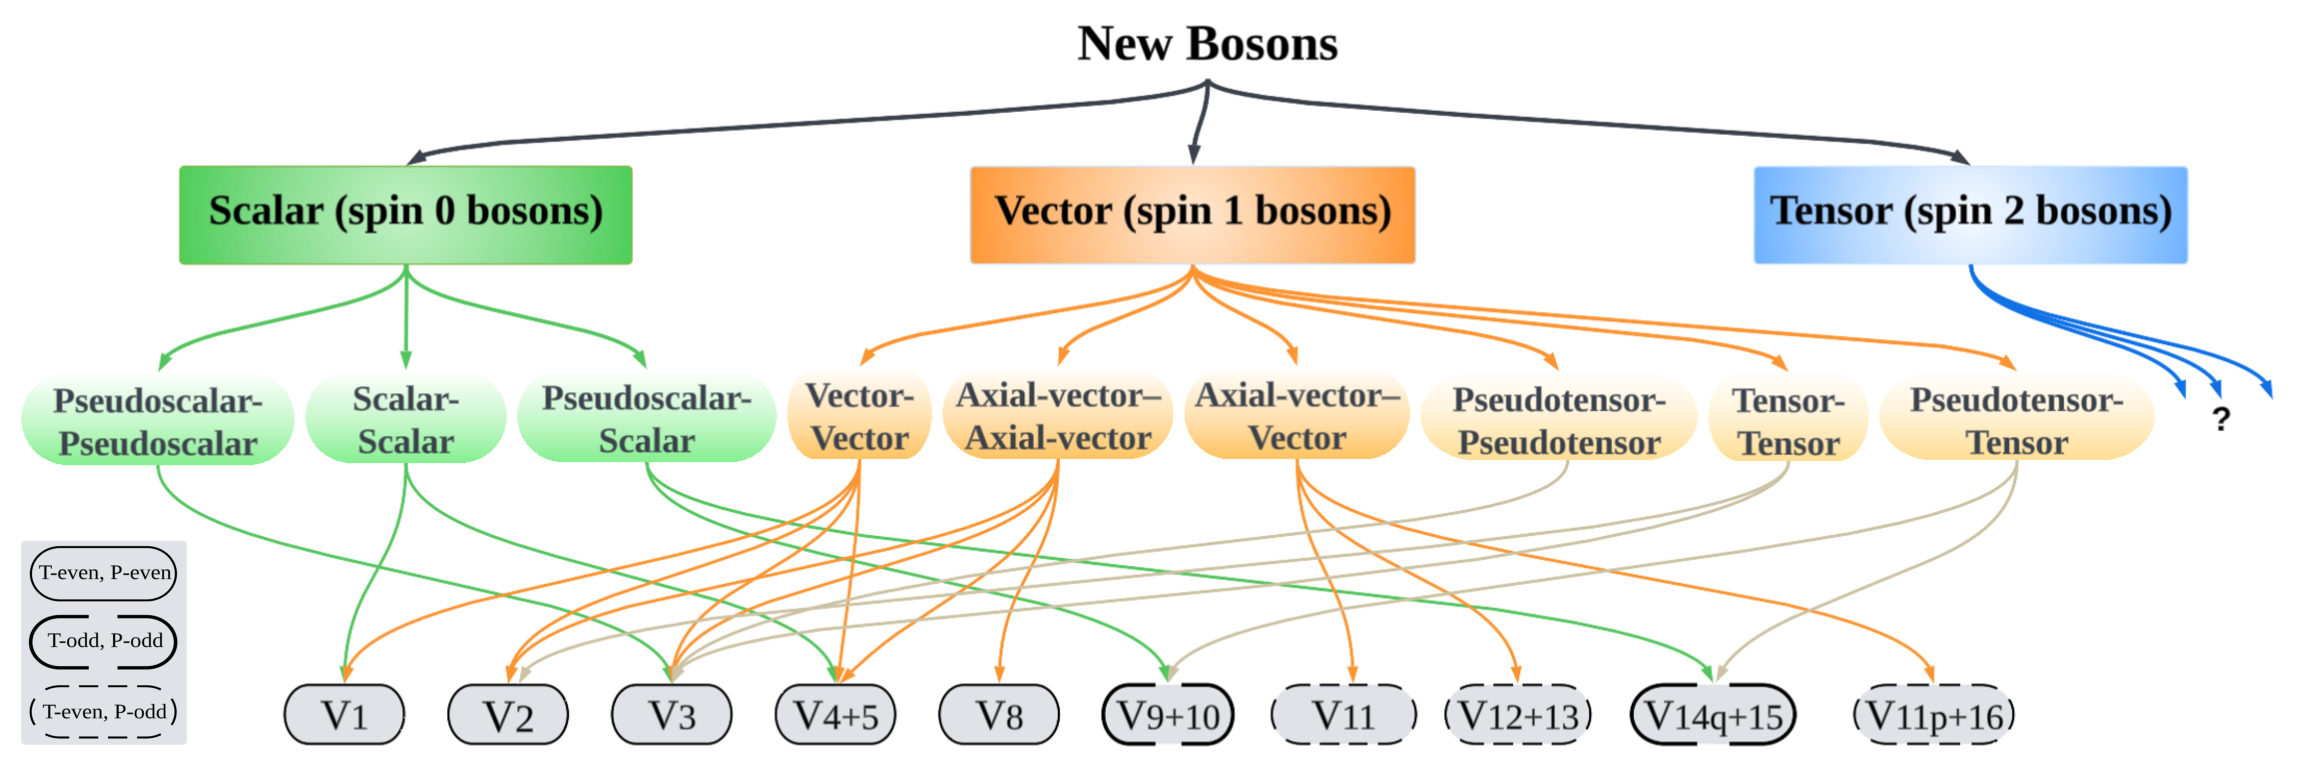
\includegraphics[width=1\textwidth]{Fig2.eps}
\end{center}
\caption{(color online). 
New bosons carrying exotic interactions between fermions. 
The green blocks in the left (the branch with scalar spin-0 bosons) were studied by \citet{moody_new_1984}. 
The potentials $V_i$ in the bottom row are related to $\sV_i$ originally proposed by \citet{dobrescu_spin-dependent_2006} and widely studied by many experiments, see Sec.\,\ref{Sec:formalism} and \ref{Sec:limits_main}. 
This latest theoretical framework provides an overview of the classification of boson potentials. \LC{See the discussion of T-odd, P-even potential in Sec.\,\ref {METH2.TOPE}.}} 
\label{New-bosons}
\end{figure*}

Based on this framework, in the results section (Sec.\,\ref{Sec:limits_main}), we discuss which potential terms $\sV_i$ provide the most stringent bounds for a particular combination of couplings. 
Generally speaking, the most stringent bounds come from the lowest-order terms like $V_2$ or $V_3$.  
Higher-order terms like $V_{4+5}$ and $V_8$ generally give less stringent bounds, but are still useful. 
These higher-order terms probe different spin/velocity structures; in the event of a detection of a spin-dependent force, higher-order terms could be used to confirm which types of couplings the exchanged boson has. 
In addition, it is possible for a single experiment or set of measurements to be sensitive to a combination of $V_i$ potential terms \cite{fadeev_pseudovector_2022}. 

%\LCa{new version:}
%Currently, it is known that each of the four fundamental interactions or forces in nature is carried by a specific type of boson. The strong nuclear force is carried by gluons, the weak nuclear force is carried by the $Z^0$ and $W^\pm$ bosons, and electromagnetism is carried by photons. It is suspected that gravitational interactions are also carried by some type of boson.
%At the low energies that are relevant at most experimentally accessible scales, quantum gravity is described perfectly well by introducing the graviton (a massless spin-2 particle) as the mediator of the gravitational force. 
%The basics of a quantum theory of gravity at low energies were laid out in the paper \cite{feynman_quantum_1963} and the 1-loop quantum corrections to Newtonian gravity have been calculated, e.g., in \citet{kirilin_quantum_2002}.


%Beyond-the-Standard-Model (BSM) theories of particle physics \cite{bagger_supersymmetry_1990,dine_supersymmetry_2023,langacker_standard_2017,farhi_technicolour_1981,dine_simple_1981,bertone_particle_2005,gunion_higgs_2000,georgi_unity_1974,panico_composite_2016,ramond_journeys_1999,shifman_advanced_2022,terning_modern_2006,weinberg_cosmology_2008,griffiths_introduction_2020} propose the existence of additional, hypothetical interactions or forces that could potentially explain a number of modern physics puzzles, such as the nature of dark matter and dark energy, the strong-CP problem, and the hierarchy problem. These theories predict the existence of new bosons that could mediate these interactions, such as axions, familons, majorons, new gravitons \cite{carroll_consequences_1994, neville_experimental_1980, neville_experimental_1982, scherk_antigravity_1979}, Kaluza-Klein zero modes in string theory, dilatons, paraphotons, and new $Z'$ bosons. 
%\DK{Should this sentence come earlier in the section??}
%\LCa{Yes,let's consider where is the suitable place to put it? Perhaps at the end of Sec.\,\ref{Sec:Intro-bg-spin}. And we add some sentence to introduce the concept of spin-dependent fifth force.}


%The concept of bosons interacting with fermions dates back to the early 20th century, when it was realized that electromagnetic interactions could be described by massless spin-1 particles known as photons. \citet{yukawa_interaction_1935} expanded on this concept to include massive spin-0 bosons, giving rise to the Yukawa potential. Additionally, in the 1960s, a low-energy quantum theory of gravity emerged, where gravitational interactions were mediated by massless spin-2 gravitons. 

%A general framework introduced by Moody and Wilczek \cite{moody_new_1984} have explored potentials resulting from the exchange of spin-0 bosons with various interactions with fermions. It is expanded by Dobrescu and Mocioiu \cite{dobrescu_spin-dependent_2006}, a different approach based on symmetries --- the symmetry-based approach predicts only the overall spin/tensor structure of potentials, but cannot uniquely predict the power-law dependence on the interparticle distance/separation. 

%It was revised in a later study by  \citet{fadeev_revisiting_2019}, allows for the study of the potential effects of these hypothetical bosons and their interactions in a unified way, regardless of the specific theories or models that predict their existence. \citet{fadeev_revisiting_2019} have chosen to sort the potentials by their types of physical couplings, in contrast to sorting them into 16 groups by their mathematical spin-momentum structure as in \cite{dobrescu_spin-dependent_2006}. This classification is more useful from a physicist’s point of view, since one is ultimately interested in the physical coupling constants of a particular model. 

%We have presented a branch diagram in Figure.\,\ref{New-bosons} showing the latest framework and how it links to \cite{dobrescu_spin-dependent_2006}'s 16 potentials. 

%This framework provides a useful tool for researchers to investigate the potential implications of these exotic interactions and their potential role in the fundamental structure of the universe.

%It's possible for a single experiment or set of measurements to be sensitive to a combination of $V_i$ potential terms.  Generally speaking, the most stringent bounds will come from the lowest-order terms like $V_2$ or $V_3$.  Higher-order terms like $V_{4+5}$ and $V_8$ will generally give less stringent bounds, but they are still useful. These higher-order terms probe different spin/velocity structures; in the event of a detection of a spin-dependent force, the higher-order terms could be used to confirm which types of couplings the exchanged boson has. 


%For more detailed description can be found in Sec.\,\ref{Sec:formalism}.


%\LCa{old version below:}
%Currently, it is known that each of the four fundamental interactions or forces in nature is carried by a specific type of boson. The strong nuclear force is carried by gluons, the weak nuclear force is carried by the $Z^0$ and $W^\pm$ bosons, and electromagnetism is carried by photons. While a satisfactory quantum theory of gravity is not yet known, \VF{it is assumed that conventional gravitational interaction is mediated by graviton, spin-2 boson. }it is suspected that gravitational interactions are also carried by some type of boson.\YS{At the low energies that are relevant to our Universe, quantum gravity is described perfectly well by introducing the graviton (a massless spin-2 particle) as the mediator of the gravitational force. The basics of a quantum theory of gravity at low energies were laid out in the paper \cite{feynman_quantum_1963}[Feynman, Acta Physica Polonica \textbf{24}, 697 (1963)] and the 1-loop quantum corrections to Newtonian gravity have been calculated, e.g., in \citet{kirilin_quantum_2002}[Khriplovich and Kirilin, J.~Exp.~Theor.~Phys.~\textbf{95}, 981 (2002)].} \DK{This is definitely a cool point about quantum gravity and the graviton. However, I wouldn't say ``relevant to our Universe'' since higher-energy physics is relevant to our Universe in terms of, at the very least, the Big Bang. Maybe ``relevant at most experimentally accessible scales'' or something like that?}

%Beyond\DKIns{-the-}Standard\DKIns{-}Model theories of particle physics propose the existence of additional, hypothetical interactions or forces that could potentially explain a number of modern physics puzzles, such as the nature of dark matter and dark energy, the strong-CP problem, and the hierarchy problem. These theories predict the existence of new bosons that could mediate these interactions, such as axions, familons, majorons, new gravitons \cite{carroll_consequences_1994, neville_experimental_1980, neville_experimental_1982, scherk_antigravity_1979}, Kaluza-Klein zero modes in string theory, dilatons, paraphotons, and new $Z'$ bosons. \DK{Should this sentence come earlier in the section??}

%\YS{We should update this paragraph to be consistent with the updated text in Sec.\,\ref{Sec:formalism} below --- in particular, the 1984 Moody-Wilczek paper wasn't the first to introduce the framework based on particle exchange, while the approach of Dobrescu-Mocioiu was a different approach based on symmetries --- the symmetry-based approach predicts only the overall spin/tensor structure of potentials, but cannot uniquely predict the power-law dependence on the interparticle distance/separation.} \DK{Agree! Great points.}
%A general framework introduced by Moody and Wilczek \cite{moody_new_1984}, expanded by Dobrescu and Mocioiu \cite{dobrescu_spin-dependent_2006}, and revised in a later study by  \citet{fadeev_revisiting_2019}, allows for the study of the potential effects of these hypothetical bosons and their interactions in a unified way, regardless of the specific theories or models that predict their existence. This framework provides a useful tool for researchers to investigate the potential implications of these exotic interactions and their potential role in the fundamental structure of the universe.

%\LC{Particles which might transmit such interactions are starting to be referred to generically as WISPs (weakly interacting sub-eV particles) [3]” (Yan and Snow, 2013, p. 1)}

%\LC{Perhaps we can change the figure to fit our latest theoretical frame because this one is for \citet{dobrescu_spin-dependent_2006} frame. }
%\DK{I love this figure! How about two diagrams in one figure (one below the other), one for the Dobrescu-Mocioiu framework and one for the Fadeev et al. framework. I think that would be ideal and super helpful!} \LCa{Sure. We can discuss about this. }


%%%%
\subsection{Experimental searches for a fifth force}
\label{Sec:Intro-Exp}

There are two search philosophies: one is to make a precise comparison of experiment and theory, for instance, in the values of transition frequencies. The other is to look for interactions that are forbidden by some symmetries, for instance, parity (P) and/or time-reversal (T) invariance, or interactions that follow a specific, unusual, dependence of the interaction on particle distances, velocities and spins. The tell-tale symmetry violation or signature are powerful tools to identify the sought-after interaction
%from inevitable 
from the usual standard-model interactions. For such searches, it is more essential to have high sensitivity rather than high accuracy of the measurements (e.g., precise calibration of the apparatus). To reveal the specific signature of the force with respect to symmetries and parameter dependences, 
one benefits from the optimized design of the force sources and sensors, including proper reversals or modulations, with a representative example being the dedicated spin sources discussed in Sec.\,\ref{METH1.SOUR.} and \ref{METH1.SENS.}.
Both types of approaches have been highly productive in the search for exotic spin-dependent interactions, as discussed in this review, Sec.\,\ref{Sec:EXP.METH.1} and \ref{EXP.METH.2}.

% \LC{Need a link to Sec.\,\ref{EXP.METH.2}. Where shall we insert it?}


% \DK{ In the above, is the phrasing ``high relative precision'' what we want? In my understanding, precision and sensitivity are somewhat interchangeable, maybe the word we are looking for is ``accuracy'' which does imply that we need to be able to get a correct absolute value out of the measurement. A point to perhaps emphasize more explicitly is that when one searches for a symmetry-respecting interaction, commonly the signal is contaminated by relatively large backgrounds that must be dealt with either through auxiliary measurements or through accurate comparison of measurements to theory. In the case of a symmetry-violating interaction, backgrounds from, e.g., electromagnetic interactions are suppressed.}


% \LC{Precision refers to the degree to which a measurement is reproducible or consistent. In other words, it describes how close a series of measurements of the same quantity are to each other. For example, if a measurement is very precise, then multiple measurements of the same quantity would yield similar results. Precision is often quantified using the concept of uncertainty, which is a measure of how much the measurements may vary from each other.}

% \LC{Sensitivity, on the other hand, refers to the ability of a measurement to detect small changes or differences in a quantity. In other words, it describes how accurately a measurement can distinguish between two different values of a quantity. For example, a measurement with high sensitivity would be able to detect small changes in a quantity, even if the overall value of the quantity remains the same. Sensitivity is often quantified using the concept of the minimum detectable difference, which is the smallest difference between two values that can be reliably detected by the measurement.}

%\WJ{ Experimental Methods, we can include: NV method for mum scale \cite{rong_constraints_2018},  comagnetometer for cm scale \cite{vasilakis_limits_2009}, Torsion Pendulum, Eot-wash, for mum-km scale. (UW latest paper sketch) 4,  Atomic spectroscopy (One of the latest best results, for instance, Physics Letters B 678 (2009) 55–59 that Philip cited), 5, parity violation \cite{antypas_isotopic_2019}}


%\subsubsection{Early experiments}\label{Sec:Intro-Exp-Ear}
%Many early experiments searched for fifth forces by testing the inverse-square law of Newtonian forces and electrostatic force which are spin-independent. We do not systematically discuss these searches here and refer the readers to a comprehensive review by \citet{adelberger_tests_2003}.

%Early experimental work on the search for new dipole interactions focused on studying the electric dipole moment (EDM) of neutrons, nuclei, and electrons. 
% The EDM is a measure of the alignment of the charge distribution within a particle with its intrinsic angular momentum and can provide information about the existence of particular types of dipole couplings. 
%Later, attention turned to the role of spin in gravity. 
%For example, \citet{morgan_direct_1962} proposed a test of the equivalence principle for a spin-polarized body, while \citet{leitner_parity_1964} showed that a gravitational monopole-dipole interaction would violate the $P$ and $T$ symmetries. If such an interaction existed, the energy of a particle would depend on the orientation of its spin relative to the local gravitational field. 
%Since no such dependence was observed, the authors were able to derive constraints on monopole-dipole couplings based on the absence of gravitationally-induced splitting of Zeeman sublevels in measurements of the ground-state HFS 
%\DB{Is this acronym defined?}\LC{yes}of hydrogen. Later experiments by \citet{wineland_atomic_1972}, which measured the ground-state hyperfine interval in atomic deuterium, and \citet{ramsey_tensor_1979}, which analyzed molecular hydrogen H$_2$ spectroscopy data, used more sensitive techniques to investigate these interactions, establishing tighter constraints on their existence.

%\subsubsection{Recent experiments}
%\label{Sec:Intro-Exp-Rec}


%Shortly after \citet{moody_new_1984} proposed three forms of new interactions induced by axions, a variety of dedicated experiments were conducted to search for these.The theoretical extension by \citet{dobrescu_spin-dependent_2006} to the 16 possible interaction terms further stimulated the experimental searches, extending then to  additional terms such as the velocity-dependent ones. Various lab-based sensors are used, for instance atomic magnetometers \cite{chu_experimental_2020,ji_constraints_2023}, atomic comagnetometers\cite{vasilakis_limits_2009,wei_constraints_2022}, NV centers in diamond \cite{rong_constraints_2018}, mechanical sensors like torsion pendulums \cite{adelberger_improved_2013} and cantilevers \cite{ding_constraints_2020}, etc. The experiments mostly involve stable fermions: neutrons in stable nuclei, protons and electrons, however some relatively rare fermions such as antiprotons, positrons, and muons are also considered in recent years \cite{fadeev_pseudovector_2022,kotler_constraints_2015,yan_constraining_2019}.  
%\LC{This part overlaps with Sec. V. A. Need to write from a different angle. Perhaps more general discussion here. } 

%The search scale ranges from the solar and earth scale to atomic scale. For the large scales, for instance \citet{heckel_preferred-frame_2008,wu_new_2023} considered the Sun and the Moon as remote mass sources, i.e. that contribute unpolarized fermions, and \citet{wineland_search_1991,venema_search_1992,jackson_kimball_constraints_2017,zhang_search_2023} considered the Earth as the mass source, while \citet{hunter_using_2013,hunter_using_2014} considered the Earth as electron spin source by taking into account its geoelectron polarisation. For the lab-scale from around 1\,cm to 100\,m, various specially designed sources are used, for instance that of spin-polarized nucleon sources \citet{glenday_limits_2008,vasilakis_limits_2009} and electron sources \cite{terrano_short-range_2015,ji_new_2018}, as well as spin-unpolarized mass sources made from high mass density materials\cite{wei_constraints_2022,tullney_constraints_2013,lee_improved_2018}. Shorter range at sub-cm are conducted using microscale sensors, for instance the mechanical sensors\cite{ding_constraints_2020} and NV-in diamond sensors\cite{rong_constraints_2018} with the sources miniaturized accordingly. The atomic scale forces are mostly investigated by precision comparison type, i.e. compare the theoretical and experimental results and try to find discrepancy induced by the new forces. These works include the ones that use the collision of  atomic vapor cells \cite{jackson_kimball_constraints_2010} and the ones with precision spectroscopy of atoms\cite{fadeev_pseudovector_2022,ficek_constraints_2017}. Neutron beam work as also investigated for the short range from millimeter to picometer dedicated experiments \cite{haddock_search_2018,voronin_neutron_2009}. 
%Details of the principles of these experiments are explained in Sec.、，\ref{Sec:EXP.METH.1} and Sec.\,\ref{EXP.METH.2}, and the results on the specific coupling are explained in the results section Sec.\,\ref{Sec:limits_main}

%The concept of a fifth force or interaction is an idea that has been proposed in the field of particle physics to explain particular experimental observations that cannot be explained by the four known fundamental forces of nature. 
%\YS{I think we have a similar phrase about the four forces of nature earlier on in the introduction. I'm also not entirely sure if the idea of fifth forces originates from particle physics. The notion of fifth forces might have been discussed in the context of scalar-tensor theories of gravity as far back as the early 20th century; there may be some relevant historical discussion and early references, e.g., in the book \url{https://www.cambridge.org/core/books/scalartensor-theory-of-gravitation/CE08614207F03739B8E0D38F90C67EFC}.} 
%In order to better understand the potential properties and implications of a fifth force, physicists have been conducting experiments and making precise comparisons between experimental data and theoretical predictions. 
%This can help to identify any inconsistencies between the data and the predictions of existing theories and to identify possible signatures of a fifth force.

%There are two main approaches that are commonly used in the search for a fifth force. 
%The first approach involves making precise comparisons between experimental data and theoretical predictions, such as by comparing the values of transition frequencies. 
%This approach relies on high precision in the measurements and calculations, in order to identify any small deviations from the predictions of existing theories. 
%The second approach involves looking for interactions that are forbidden by particular symmetries, such as parity ($P$) and/or time-reversal ($T$) invariance. 
%In this latter approach, it is more important to have high sensitivity in the measurements since the effect is expected to be very small.
%, in order to detect small deviations from the expected behavior. 
%\YS{I think the argument here isn't necessarily valid. For example, even if the SM predictions for the EDMs of particles and atomic systems are practically zero (which is the case), it's in principle possible for the new-physics contribution to be many orders of magnitude larger than the SM contribution. Of course, measurements of ever increasingly high sensitivity are desirable, but this is in part because the current experimental limits on EDMs are already extremely stringent.}
%Both of these approaches have been used to search for exotic spin-dependent interactions, and they have yielded valuable insights into the potential properties of a hypothetical fifth force.
%\MK{The text above overlaps with Sec.\ I.D.1 General remarks.}

%Even though current experiments have not yet unambiguously observed 
%cannot confirm the existence of 
%a fifth force, constraining the properties of a fifth force can also help to eliminate particular explanations that are ruled out by the data \YS{I'm not sure I understand the meaning of this phrase}, and this can help to guide future research and experiments. For example, if an experiment were to show that a fifth force must have a certain range or strength in order to be consistent with the data, this could help to narrow down the possible mechanisms for the fifth force and to guide the development of new theories and models. In addition, constraints on the properties of a fifth force can help to identify the energy scales at which a fifth force is likely to become significant, and this can inform the design of future experiments and observations that aim to detect the fifth force.

%However, it is important to note that the research on fifth forces is still in its early stages \YS{I'm not sure if it's entirely accurate to describe a (roughly) century-old field as still being in its early stages - since this subsection is about recent experiments, maybe we could instead say that there has been (somewhat of) a Renaissance in recent years in terms of novel and more precise experimental probes being devised to search for fifth forces?}, and much more work is needed to fully understand its possible properties and implications. 
%While there are many observations and experimental results that suggest the existence of a fifth force, there is currently no direct evidence for its existence. 
%Consequently, the notion of a fifth force continues to be a theoretical hypothesis, necessitating further research and experimentation to either validate or disprove specific models of this proposed force.
%\YS{This may be a philosophical discussion, but I don't think it's possible to entirely rule out the concept of a fifth force in the broad and general sense. In principle, we might be able to rule out certain (classes of) models that are capable of producing fifth forces.}

\subsection{Discrete-symmetry-violating and -respecting interactions }

A general aspect of exotic long-range spin-dependent interactions to consider is whether they respect discrete symmetries such as charge-conjugation $C$, parity $P$, and time-reversal $T$. 
The weak interaction, for example, violates $P$ and also the combined symmetry $CP$.
On the other hand, the electromagnetic interaction respects $C$, $P$, and $T$.

The advantage of searching for discrete-symmetry-violating interactions is that background effects from the SM are strongly suppressed, as the short-range weak interaction is the only known symmetry-violating interaction in the SM.
On the other hand, searches for symmetry-respecting interactions offer the opportunity to directly constrain particular unknown coupling constants that cannot be directly constrained otherwise.
The idea is as follows. 
All of the long-range exotic potentials discussed here involve two coupling constants: one from the vertex representing the local interaction at the source and one from the vertex representing the local interaction at the sensor.
Symmetry-violating effects arise due to the involvement of two vertices with different symmetry characteristics. 
An example from the SM is the $P$-violating weak interaction that involves a vector and axial-vector coupling.
Thus an experimental measurement constraining a new symmetry-violating interaction necessarily only limits the product of two \emph{different} coupling constants, $g^Xg^Y$.
Such an experiment by itself does not constrain the individual coupling constants $g^X$ and $g^Y$ since one of them could be, for example, zero, and then the other is completely unconstrained by the measurement.
On the other hand, new symmetry-respecting interactions can be generated by local interactions of the same character and involve the square of a coupling constant $g^Xg^X$.
An experimental measurement constraining a new symmetry-respecting interaction provides a direct limit on a particular coupling constant $g^X$.

A similar point can be made for experiments measuring cross-species interactions as compared to same-species interactions. 
An experiment searching for an exotic interaction between electrons can constrain the square of the electron coupling constant, $g^eg^e$, and thus directly constrain $g^e$ itself, whereas an experiment searching for an exotic interaction between neutrons and electrons only constrains a product of coupling constants $g^eg^n$. Since either $g^n$ or $g^e$ could be zero, the experiment provides no direct constraint on the individual coupling constants.

Notably, the above argument can be usefully reversed, as discussed, for example, by \citet{raffelt_limits_2012}.
\citet{raffelt_limits_2012} took constraints on a scalar axion coupling $g_s$ from symmetry-respecting long-range force measurements and combined these with astrophysical constraints on the axion pseudoscalar coupling $g_p$ to constrain the product of coupling constants $g_sg_p$.
While many experiments have searched for long-range $P$- and $T$-violating monopole-dipole interactions proportional to $g_sg_p$, the constraints obtained by \citet{raffelt_limits_2012} remain among the most stringent. 

In this review, we present combined astrophysical-laboratory bounds for comparison with direct bounds from experiments; see figures in Sec.\,\ref{Sec:limits_main} and for more details, App.\,\ref{appendix_comp.}.


%\subsection{Expected impact of a fifth-force discovery }\label{Sec:Intro-impact}

%The study of fifth forces has the potential to greatly impact our understanding of nature. 

%If forces beyond the four known fundamental ones are found to exist, this would result in a major shift in our understanding of the fundamental laws of physics. This, in turn, could spur the development of new technologies, such as sensors and detectors (see Sec.\,\ref{Sec:EXP.METH.1}).%, to measure these forces more accurately.

%Furthermore, the existence of the fifth forces could have implications for our understanding of the universe itself. 
%\YS{For example, theories with extra dimensions predict highly singular fifth forces on short length scales; see, e.g., [Arkani-Hamed, Dimopoulos, Dvali, Phys.~Lett.~B \textbf{429}, 263 (1998); Phys.~Rev.~D \textbf{59}, 086004 (1999)].}
%For example, theories with extra dimensions predict highly singular gravitational forces on short length scales; see, for example, \citet{arkanihamed_hierarchy_1998,arkani-hamed_phenomenology_1999}. 
%At subatomic distances, these forces may be probed by comparing measured and calculated spectra of simple atomic and molecular systems [as referenced in recent papers by (\citealp{salumbides_constraints_2015}; \citealp{dzuba_effects_2022}) and further discussed in Sec.\,\ref{EXP.METH.2}].
%If these forces are confirmed, it could provide evidence for the existence of additional dimensions beyond the four we currently know. %This could lead to new theories about the fundamental structure of the universe and its origins and evolution.

%Overall, the discovery of fifth forces could provide new insights into the fundamental principles that govern the universe and have important implications for the advancement of both technology and theoretical frameworks.

%%%%
\subsection{Goals, scope and structure of this review }\label{Sec:Intro-GSS}

Our goal, after the general introduction to the topic, is to provide a concise description of the theoretical approaches to help the reader navigate through different frameworks and conventions. 
Tracing the development of the theoretical approaches, we present the latest unified approach and a set of spin-dependent interaction potentials. 
We then proceed to critically evaluate the significant body of recent experimental results, presenting the combined up-to-date\footnote{While there is no sharp cut-off, the data presented in this review are mostly those published through early 2024.} constraints on exotic interactions. 
The unified theoretical description enables a systematic comparison of results obtained in different experiments. 
Finally, we identify promising directions for future experimental work and discuss the significance and impact of a possible discovery.   

To limit the scope of the project, we focus on exotic spin-dependent interactions, only discussing the spin-independent ones when necessary for logical completeness and to compare the results for couplings that produce both types of interactions. 
Comprehensive reviews of spin-independent interactions can be found elsewhere (\citealp{adelberger_torsion_2009}; \citealp{antoniadis_short-range_2011}; \citealp{heil_spin_2013}; \citealp{salumbides_bounds_2014}; \citealp{lemos_submillimeter_2021}).
%\cite{lemos_submillimeter_2021,salumbides_bounds_2014,antoniadis_short-range_2011,heil_spin_2013,adelberger_torsion_2009}. 

Another limitation on the scope is that we consider results in the nonrelativistic limit and largely stay away from the domain of high-energy physics \cite{boveia_dark_2018}.

While spin-dependent interactions were discussed in earlier reviews, e.g., that by \citet{vergeles_general_2023}, the most relevant earlier review is that of \citet{safronova_search_2018}, which examines spin-dependent exotic interactions in Section VII of that paper. 
However, there has been an ``explosion'' of both theoretical and experimental results in the years that have passed since that review. 
Our current review is significantly broader, more complete, up-to-date, and systematic. 
%
%\LCa{From DFG proposal:}
%
%a)Critical reassessment of exotic potentials and formulation of the consistent and complete set of potentials. This will ensure all possible interactions are suitably considered.
%
%b)Formulation of the potentials in terms of a small number of coupling constants (as shown in work Package III). This will help to streamline the comparison of different experimental results and maximize the impact of each study.
%
%c)Critical assessment of the entire body of experimental literature on spin-dependent exotic interactions to generate exclusion plots and projected sensitivity. This will facilitate a more cohesive understanding of the current research landscape.

The paper is organized as follows. In Sec.\,\ref{Sec:formalism}, we review the theoretical frameworks for spin-dependent exotic interactions. 
In Sec.\,\ref{Sec:EXP.METH.1}, we focus on dedicated source-sensor experiments, while in Sec.\,\ref{EXP.METH.2}, we discuss complementary experiments and observations for detecting exotic spin-dependent interactions. 
In Sec.\,\ref{Sec:limits_main}, we categorize the current best or most recent limits on spin-dependent potentials and coupling constants, based on the latest theoretical framework. 
Sec.\,\ref{Sec:Sum-Out} provides a summary and outlook.


%Modern physics acknowledges the existence of four fundamental interactions -- strong, weak, electromagnetic, and gravitational. They vary in strengths and ranges, and for different physical systems some of them may be more important than the others (for example strong interactions inside baryons or gravitational interactions in the galaxy). In spite of the fact that there is no direct proof of existence of any other fundamental interaction (although there are many observations suggesting their existence, as we discussed in the next section), there is in principle no argument ruling out such a possibility. Instead, one can only constrain strengths of such hypothetical interactions using precise experimental measurements.
% \WJ{In this paper, we focus on laboratory results and put as much other results as possible, such as astrophysical results. It is worth noticing that the astrophysical limits use varies assumptions on conditions that are not well known or defined to derive some limits. Laboratory experiments are directly results and thus more solid. }


%\begin{itemize}
    %\item \DB{Why exotic interactions (new particles); history of classification (Moody Wilzcek, Dobrescu, Fadeev et al)}
    %\item \DB{A lot of recent experiments motivated by BSM searches and DM searches; need to compare the reach of different experiments}
    %\item \DB{Successful couch physics: He, antiprotonic He, etc.}
   % \item \DB{The structure of this review: }
    
    % \item \DB{The way I see it, we should look at the potentials one by one and, following Victor’s approach, ask: what system could be most sensitive to this particular type of interaction? Then we go and see:}\\


   %  \item \DB{Has it been used to constrain these particular couplings? If yes---report in the paper. If no,}\\

 %\item \DB{What are the most precise experimental results and what is the most precise theory?}\\

 %\item \DB{Do the “couch” analysis and set constraints\\Report in the paper.}\\

%\LCa{for \cite{fadeev_pseudovector_2022} hydrogen HFS e-p constraints, new experiment result \cite{bullis_ramsey_2023}. }

%\item \DB{We limit ourselves to spin-dependent interactions. Spin-independent interactions are discussed in a number of references \cite{}}


%\item \DB{We need to remember to add a discussion of us always taking the minimalistic assumption of a single source for the exotic interactions (e.g., a new vector boson). In principle, this could be wrong as pointed out in the case P,T-odd electric-dipole-moment (EDM) searches \cite{chupp_electric_2015}. However, it is our opinion that the minimalistic framework is appropriate until the time an exotic interaction is discovered.} \LCa{move to Sec.\ref{Sec:Intro-Th}?}
%\end{itemize}
%
%\FF{Modern physics acknowledges the existence of four fundamental interactions -- strong, weak, electromagnetic, and gravitational. They vary in strengths and ranges, and for different physical systems some of them may be more important than the others (for example strong interactions inside baryons or gravitational interactions in the galaxy). In spite of the fact that there is no direct proof of existence of any other fundamental interaction (although there are many observations suggesting their existence, as we discussed in the next section), there is in principle no argument ruling out such a possibility. Instead, one can only constrain strengths of such hypothetical interactions using precise experimental measurements.}

%\LC{check the hidden part below}
%\FF{At this moment we know that every fundamental interaction, except gravity for which a satisfactory quantum theory is not yet known, is carried by some interacting bosons -- photons for electromagnetic, gluons for strong, and $Z^0/W^\pm$ bosons for weak interactions. We suspect that exotic interactions also would be carried by some, yet undiscovered bosons. Many modern physics puzzles, such as the nature of dark matter \cite{bernet_spiral_2005} and dark energy \cite{Fri03,Fla09}, the strong-CP problem \cite{moody_new_1984}, or the hierarchy problem \cite{graham_experimental_2015}, may be explained by Beyond Standard Model theories predicting existence of such new bosons. The Examples include axions \cite{Wei78,Wil78,Din81,Shi80,Kim79,Zhi80}, familons \cite{Wil82,Gel83}, majorons \cite{Gel81,Chi81}, new spin-0 or spin-1 gravitons \cite{Sch79,Nev80,Nev82,Car94}, Kaluza-Klein zero modes in string theory \cite{Svr06}, paraphotons \cite{Oku82,Hol86,Dob05}, and new $Z'$ bosons \cite{Bou83,App03,Dzu17}. Despite the different nature of all these particles and the reasons the corresponding models were proposed, interactions they carry may be described within one, general framework introduced by Moody and Wilczek \cite{moody_new_1984}, expanded by Dobrescu and Mocioiu \cite{dobrescu_spin-dependent_2006} and revised in \cite{fadeev_revisiting_2019}.}




%%%%%%%%%%%%%%%%%%%%%%%%%%%%%%%%%%%%%%%%%%%%%%%%%%%%%%
                 % Sec-Theory
%%%%%%%%%%%%%%%%%%%%%%%%%%%%%%%%%%%%%%%%%%%%%%%%%%%%%%

%%%%%%%%%%
\section{Theoretical frameworks}
\label{Sec:formalism}

%%%%%%%%%%%%%%%%%%%%%%%%%%%%%%%%%%%%%%%%%%%%%%%%%%%%%%
                      % The1. Early formalisms
%%%%%%%%%%%%%%%%%%%%%%%%%%%%%%%%%%%%%%%%%%%%%%%%%%%%%%
\subsection{Early developments}
\label{Subsec:MWformalism}

%Generally speaking, the most commonly employed framework for the purpose of comparing different experimental searches for exotic spin-dependent interactions is that introduced by \citet{moody_new_1984} to describe spin-dependent potentials. This framework provides a means of detecting Axion (very light spin-0 bosons) through the macroscopic forces they mediate. 
%The possible forces are determined by the two kinds of couplings to fundamental fermions: the scalar vertex and the pseudoscalar vertex. \citet{moody_new_1984} formulated three combinations of the scalar and pseudoscalar vertices that can appear in one-boson-exchange graphs: namely monopole-monopole, monopole-dipole, and dipole-dipole, which are denoted as $\sV_1$, $\sV_{9+10}$, $\sV_3$ respectively in the Dobresu and Mociau formalism in the next subsection. 
%The latter two are spin-dependent interaction and inspired a series of research. 

%Generally speaking, the most commonly employed framework for the purpose of comparing different experimental searches for exotic spin-dependent interactions is that introduced by \citet{moody_new_1984}. This framework describes spin-dependent potentials and provides a means of detecting Axion (very light spin-0 bosons) through the macroscopic forces they mediate. \citet{moody_new_1984} proposed that the possible exotic forces are determined by the two kinds of couplings to fundamental fermions: the scalar vertex and the pseudoscalar vertex. \citet{moody_new_1984} formulated three combinations of the scalar and pseudoscalar vertices that can appear in one-boson-exchange graphs: namely monopole-monopole, monopole-dipole, and dipole-dipole, which are denoted as $\sV_1$, $\sV_{9+10}$, $\sV_3$ respectively in the later Dobresu and Mociau formalism, as shown in the next subsection. The latter two are spin-dependent potentials. However, even though \citet{moody_new_1984}'s work inspired a series of studies about spin-dependent interaction, compared to spin-independent one $\sV_1$ \cite{antoniadis_short-range_2011,long_current_2003,kapner_tests_2007,adelberger_tests_2003,costantino_exotic_2020}, the spin-dependent interaction have received less attention before \citet{dobrescu_spin-dependent_2006}, even though they could lead to a broader variety of observable effects. 

%\YS{I don't think this statement is entirely accurate and I don't think it's appropriate that the formalism should be (entirely) attributed to Moody and Wilczek. 
%Very similar frameworks for describing inter-particle potentials associated with the exchange of a boson have been considered earlier. 
%For example, the scalar-scalar potential was considered in the seminal paper [Yukawa, Nippon Sugaku-Buturigakkwai Kizi Dai 3 Ki \textbf{17}, 48 (1935)], the scalar-pseudoscalar potential was considered in [Bouchiat, Physics Letters \textbf{57B}, 284 (1975)], and the pseudoscalar-pseudoscalar potential was considered in [Ansel'm, JETP. Lett. \textbf{36}, 55 (1982); Pis'ma Zh. Eksp. Teor. Fiz. \textbf{36}, 46 (1982)]. 
%There may have been other papers prior to the 1984 paper of Moody and Wilczek.  
%The papers of Bouchiat, Ansel'm and Moody-Wilczek all discussed some (novel) the searching for such potentials.}

%\LC{Those papers \cite{anselm_possible_1982-2, bouchiat_limit_1975, yukawa_interaction_1935} seems are not well cited by the papers in the spin-dependent fifth force field. How about we discuss them more in the introduction part and briefly here and still emphasize the \cite{moody_new_1984} is the most common framework in this Section?} 

%\LC{\citet{anselm_possible_1982-2} has been mentioned in the Introduction : "Subsequently, the appearance of the idea of spin-dependent potentials generated by light spin-0 particles, such as axions \cite{moody_new_1984} and arion \cite{anselm_possible_1982-2}, sparked interest in searches for exotic spin-dependent interactions." pseudoscalar-pseudoscalar }
%\LC{\citet{bouchiat_limit_1975} EDM, scalar-pseudoscalar potential}

%{\color{red} PF: Text below edited according to the remarks above.}

%\YS{Thank you for clarifying. In this case, maybe we could call this subsection something like ``Early history/developments'' and recount the early developments starting from Yukawa's paper, then leading up to the Moody-Wilczek paper, followed by a brief discussion of experimental efforts?}

%In general, the most common framework for comparing different experiments searching for exotic spin-dependent interactions was introduced by \citet{moody_new_1984}. 
%\LC{Ok.} 

%\LC{In 1935, \citet{yukawa_interaction_1935} first introduced the concept that the interaction of elementary particles can be described by a hypothetical quantum that has the elementary charge and the proper mass and which obeys Bose's statistics. Such interactions are referred to as Yukawa-type interactions. One of the most well-known examples of a Yukawa-type interaction is the interaction between nucleons (protons and neutrons) in the nucleus, which is mediated by the exchange of mesons. }

%\YS{I've expanded on the introductory part on the early developments and concepts, and updated the existing paragraph\LC{checked, accept}, please check.}

%\LC{Thank you so much.}
\iffalse
\VF{ I believe discussion of Coulomb, magnetic  and Newton laws should be removed. Again,  elementary school staff. Please, delete between ???}

???????


The study of fifth forces acting ``at a distance'' dates back to studies of falling bodies and the motions of astrophysical bodies in the early 17th century in the context of gravity. 
Gravitational interactions \cite{will_theory_2018} between two bodies of masses $M_1$ and $M_2$ can be described by the Newtonian potential $V = - G M_1 M_2 / r$ in the nonrelativistic limit, where $G$ is the gravitational constant and $r$ is the interbody separation. 
Gravity involves only ``like'' charges and is always attractive. 
This implies that gravitational effects can accumulate enormously on macroscopic and astronomical scales, and so gravity tends to be the dominant force on astronomical length scales. 

Studies of electromagnetic forces began to take prominence starting from the late 18th century. 
%Coulomb's law \cite{feynman_feynman_2011}, in particular, describes the electrostatic interaction between two electrically charged particles of charges $Q_1$ and $Q_2$ according to $V = -k Q_1 Q_2 / r$, where $k$ is the Coulomb constant. 
Coulomb's law \cite{feynman_feynman_2011}, in particular, describes the electrostatic force between two electrically charged particles. The associated electric potential energy between these charges is given by 
$V = -k \frac{Q_1 Q_2}{r}$, where $k$ is the Coulomb constant, and $ Q_1 $ and $ Q_2 $ are the charges.
Unlike ``unsigned'' particle masses, electric charges are ``signed'' quantities, which implies that the Coulomb force can be either attractive or repulsive. 
%Due to the overall electrical neutrality of the Universe and atoms, the Coulomb force tends to be effectively screened on macroscopic scales, even though the Coulomb force is intrinsically many orders of magnitude stronger than the gravitational force. 
Unlike the build up of gravitational force, there is usually no build-up of electric force as opposite charges in equilibrium do not tend to produce a noticeable electric field in the far-field limit. % suggested revision by Pasha
Additionally, magnetic interactions of a dipolar character arise between particles possessing magnetic moments. 


??????
\fi

During the development of quantum field theory in the early 20th century, it was realized that electromagnetic interactions could be described in terms of the exchange of a massless spin-1 mediator known as the photon \cite{peskin_introduction_2019}. 
Later, Yukawa generalized this concept to massive spin-0 bosons, the exchange of which gives rise to the Yukawa potential $V = -g^2 \exp(-M r)/ (4 \pi r)$, where $g$ is the dimensionless coupling constant and $M$ is the mass of the exchanged boson \cite{yukawa_interaction_1935}. 
In this case, the exchanged boson could in principle be either elementary or composite; in both cases, the exchanged boson can be treated as a single spin-0 degree of freedom on the length (or equivalently energy) scales involved. 
In the SM, for example, the strong nuclear force is mediated between nucleons by the exchange of pions and other mesons.
%, which are composite bosons made up of quarks and anti-quarks. 

A low-energy quantum theory of gravity, in which gravitational interactions are mediated by the exchange of a massless spin-2 graviton, was developed in the 1960s %\LC{Shall we cite some reference here, e.g. 
(\citealp{feynman_quantum_1963}; \citealp{penrose_zero_1965}; \citealp{dewitt_quantum_1967}).
%\cite{feynman_quantum_1963,dewitt_quantum_1967,penrose_zero_1965}. 
%\DK{Yes, a reference here would be great!}

Since then, a number of studies of potentials induced by the exchange of exotic bosons have been undertaken. 
\citet{bouchiat_limit_1975} investigated the \textit{P},\textit{T}-odd potential arising from the exchange of a spin-0 boson, which interacts with one fermion via a scalar-type vertex and with another fermion via a pseudoscalar-type vertex. 
\citet{anselm_possible_1982} investigated the dipole-dipole potential arising from the exchange of a spin-0 boson that couples to fermions via a pseudoscalar-type vertex. 
\citet{moody_new_1984} explored the potentials arising from the exchange of a spin-0 boson that possesses both scalar and pseudoscalar-type interactions with fermions. 
In this case, three qualitatively different combinations of vertex types are possible, namely scalar-scalar, scalar-pseudoscalar and pseudoscalar-pseudoscalar. 
These lead, respectively, to monopole-monopole, monopole-dipole and dipole-dipole potentials/forces. 
The first of these is spin-independent at leading order and corresponds to the potential term $\mathcal{V}_1$ in the notation presented later on in Sec.\,\ref{Subsec:DMformalism}, see Eq.\,(\ref{DM_eqV1}). 
The latter two are already spin-dependent at leading order and correspond to the potential terms $\mathcal{V}_{9+10}$ and $\mathcal{V}_{3}$, respectively, see Eqs.\,(\ref{DM_eqV910}) and (\ref{DM_eq3}). 

%In 1984 \citet{moody_new_1984} discussed the application of exotic boson-exchange potentials as macroscopic forces. 
%In so doing, \citet{moody_new_1984} was one of several papers noting various implications of one-boson exchange potentials \cite{anselm_possible_1982-2, bouchiat_limit_1975, yukawa_interaction_1935}. 
%The paper \citet{moody_new_1984} describes the spin-dependent potential and provides a way to detect axions (very light spin 0 bosons) via axion-mediated macroscopic forces.
%\citet{moody_new_1984} propose that possible exotic forces are determined by two types of couplings to elementary fermions: scalar vertices and pseudoscalar vertices. 
%\citet{moody_new_1984} formulates three combinations of scalar and pseudoscalar vertices in a single boson exchange graph: monopole-monopole, monopole-dipole, and dipole-dipole denoted as $\sV_1$, $\sV_{9+10}$, $\sV_3$ respectively in the later Dobresu and Mociau formalisms, as shown in the next Section. 
%The latter two are spin-dependent potentials. 

%\LC{The work of \citet{moody_new_1984} inspired a series of studies on spin-independent interactions, see Ref. \citet{lemos_submillimeter_2021,antoniadis_short-range_2011,long_current_2003,kapner_tests_2007,adelberger_tests_2003,costantino_exotic_2020} as well as spin-dependent interactions, such as for $\sV_{9+10}$ \citet{wineland_search_1991,ni_search_1999, ritter_search_1993,venema_search_1992,youdin_limits_1996} and \citet{baesler_constraint_2007,serebrov_new_2009, voronin_neutron_2009,hoedl_improved_2011,bulatowicz_laboratory_2013,heil_spin_2013,tullney_constraints_2013} and \citet{arvanitaki_resonantly_2014,afach_constraining_2015,stadnik_nuclear_2015,terrano_short-range_2015,crescini_improved_2017,crescini_quax-gpgs_2017,luo_proposed_2020,xiong_searching_2021,crescini_search_2022} and so on.}

%\YS{\textbf{[Alternative wording for the paragraph above]:} 
The above ideas \cite{bouchiat_limit_1975,anselm_possible_1982,moody_new_1984}, among others, inspired a generation of new experimental searches, including searches for spin-independent exotic forces [see, e.g., \citet{long_current_2003}; \citet{adelberger_tests_2003}; \citet{kapner_tests_2007}; \citet{antoniadis_short-range_2011}; \citet{costantino_exotic_2020}; \citet{lemos_submillimeter_2021}], as well as spin-dependent forces [see, e.g., \citet{wineland_search_1991}; \citet{venema_search_1992}; \citet{youdin_limits_1996} and \citet{ voronin_neutron_2009}; \citet{hoedl_improved_2011}; \citet{tullney_constraints_2013} and \citet{stadnik_nuclear_2015,terrano_short-range_2015}; \citet{crescini_improved_2017,crescini_quax-gpgs_2017,crescini_search_2022}; \citet{luo_proposed_2020}; \citet{xiong_searching_2021}]. 
In this review, we discuss the latest updates in theory and experiments.

%\LC{Thanks. I updated the references list above.}


%\LC{However, spin-dependent interactions may lead to a wider range of observable effects \citet{dobrescu_spin-dependent_2006}, as going to be described in this review.}

%\LC{Dima: certain potentials come in pairs: we need to explain why!}
%\YS{I don't recall if we ended up discussing this point in this review. It would be nice to double-check this.}

%%%%%%%%%%%%%%%%%%%%%%%%%%%%%%%%%%%%%%%%%%%%%%%%%%%%%%
                      % The2. Appro & limit
%%%%%%%%%%%%%%%%%%%%%%%%%%%%%%%%%%%%%%%%%%%%%%%%%%%%%%

\subsection{Approximations and limitations}
\label{Sec:th-AP}

In this section, we outline the limitations and approximations that we adopt in this review.\footnote{These approximation pertain to theory and interpretation of experiment; the experiments may have sensitivity to new physics going beyond these approximations, such as, for example, exotic high-spin bosons.} 
The frameworks in \citet{moody_new_1984}; \citet{dobrescu_spin-dependent_2006}; \citet{fadeev_revisiting_2019} provide 
an overview of the classification of single-boson-mediated potentials and set the stage for the investigation of the implications of these exotic interactions. 
In this review, we consider interactions between fundamental spin-1/2 fermions via the exchange of a single spin-0 or spin-1 boson. 
For example, we do not systematically discuss spin-2 boson exchange and many-boson-exchange processes. 
Let us consider in turn all the assumptions in this scenario and the limitations they may cause.

%%%
%\paragraph{The spin of the intermediate bosons.} 
\subsubsection*{1. The spin of the intermediate bosons} 
We consider only spin-0 and spin-1 mediators. This brings up several questions.
\begin{itemize}

\item Why do we consider only these?  Up to now, we do not have a consistent ultraviolet (UV)-complete theory for higher-spin bosons. 
This does not mean that they do not exist, but this is beyond our scope here.

\item Can higher-spin propagators be considered?  
An effective low-energy theory can be used to analyze interactions mediated by spin-2 bosons. One can write down the spin-2 propagator to consider the exchange of the spin-2 bosons in the first order of perturbation theory. 
The interactions of spin-2 bosons with matter can in principle take on a different form than those for spin-0 or spin-1 bosons, but that does not necessarily mean that the structures of the resulting potentials will be fundamentally different. 
For example, the exchange of a massless spin-0 boson with scalar-type interactions to matter produces the same $1/r$ form of the non-relativistic potential as the exchange of a spin-2 graviton between two masses (\citealp{feynman_quantum_1963}; \citealp{penrose_zero_1965}; \citealp{dewitt_quantum_1967}), %\cite{feynman_quantum_1963,dewitt_quantum_1967,penrose_zero_1965}, 
%\DB{ A more familiar example is that Coulomb and Newtonian gravitational potentials are the same :) Shall we mention this? }\YS{It's true that the Coulomb (spin-1 mediated) and gravitational (spin-2 mediated) potentials both have a $1/r$ form, but there is an important difference: the Coulomb potential can be either repulsive or attractive depending on the relative signs of the interacting charges, whereas the gravitational potential is always attractive (since masses don't have signs). Likewise, the spin-0 case is also attractive. If I recall correctly, there may be a general theorem about this, namely that mediators with even spin always produce attraction in this context, whereas mediators with odd spin can be either attractive or repulsive. We could give the spin-1 vs spin-2 (and spin-0) comparison at the end of this paragraph if you like.}\DB{Zhenia, I very much like this discussion and it would be great to have a summary of it in the review. But we are not sure where excatly you suggest placing it. Could you just place the corresponding sentence or two where you want it?} \YS{My suggestion would be to simply add this discussion at the end of this paragraph. I've drafted a possible wording below.}
even though the structure of their underlying couplings to matter is different in the two cases (scalar vs tensor). 
Likewise, the exchange of a spin-1 photon also leads to a non-relativistic potential with a $1/r$ form.\footnote{Unlike the attractive non-relativistic $1/r$ potential mediated by spin-0 or spin-2 boson exchange, the Coulomb potential mediated by spin-1 boson exchange may be either attractive or repulsive depending on the relative signs of the electric charges involved.} 


\item Will such propagators bring new structures of potentials? The potentials we consider here present all structures that are linear in the spin and momentum of fermions with spin $s=1/2$. 
For example, if we consider short-range (contact) interactions, then one can obtain all possible spin-dependent potential structures from combinations of $\gamma$-matrices of the interacting fermions without any reference at all to the intermediate boson \cite{khriplovich_parity_1991}. 
However, depending on the spin of the boson, the potentials can appear in particular combinations with different sets of coefficients (see Sec.\,\ref{Subsec:Fformalism}). 
\end{itemize}

%%%
\subsubsection*{2. One-boson versus two-boson or two-fermion exchange} 

Based on empirical evidence, the interaction constant associated with new forces is likely to be small, in which case two-boson exchange is strongly suppressed compared to single-boson exchange since the former process contains an extra power of a small interaction constant.\footnote{There may be processes involving the exchange of an exotic boson and a SM boson (e.g., a photon). 
Such mixed-boson-exchange processes contain another small interaction constant (e.g., $\alpha$), and so are still suppressed compared to the single-exotic-boson exchange process.} 
It may be necessary to consider such processes when single-boson exchange is suppressed by some selection rules.
However, two-fermion-exchange processes, such as neutrino-pair-exchange forces, may be important, as single-fermion exchange does not produce an inter-particle potential; see, e.g., \citet{stadnik_probing_2018}; \citet{ghosh_probing_2020};
\citet{bolton_probing_2020};
\citet{costantino_neutrino_2020}; \citet{xu_short-range_2022}; \citet{dzuba_long-range_2022}; \citet{dzuba_erratum_2022}; \citet{munro-laylim_effects_2023}. %\LC{In addition, the exchange of two bosons can generate a spin-independent contribution to the interaction energy between two fermions, allowing the constraint of spin-dependent couplings by reanalyzing data from existing spin-independent experiments \cite{aldaihan_calculations_2017}.}
%\YS{Slightly updated suggestion: 
In addition, the exchange of a pair of bosons with spin-dependent couplings to matter can generate a higher-order spin-independent contribution to the interaction energy between the two fermions, potentially allowing one to more stringently constrain spin-dependent couplings by reanalyzing data from existing experiments that search for spin-independent forces 
%\DK{add reference: Ephraim Fischbach and Dennis E. Krause, ``Constraints on Light Pseudoscalars Implied by Tests of the Gravitational Inverse-Square Law'' Phys. Rev. Lett. 83, 3593 (1999)} 
(\citealp{fischbach_constraints_1999}; \citealp{aldaihan_calculations_2017}).
%} 


%{\color{red}We can also cite the following papers here following Victor's suggestion: \url{https://journals.aps.org/prd/abstract/10.1103/PhysRevD.101.116006}, \url{https://link.springer.com/article/10.1007/JHEP07(2020)013}, \url{https://link.springer.com/article/10.1007/JHEP09(2020)122}, \url{https://journals.aps.org/pra/abstract/10.1103/PhysRevA.106.012817}, \url{https://link.springer.com/article/10.1007/JHEP02(2022)008}}


Two-boson (and two-fermion) exchange-induced potentials have different dependences on the interparticle distance compared to single-boson potentials; see, for example, \citet{bauer_fifth_2024}. 
In addition, in the case of interactions between composite systems, such as nuclei, the pair of exchanged bosons can interact with different nucleons within the same nucleus. 
This leads to an increase in the possible types of potential structures that are not necessarily limited to the forms of the potentials $V_1$ -- $V_{16}$ and related potentials containing additional integral powers of fermion momenta discussed in Secs.\,\ref{Subsec:DMformalism} and \ref{Subsec:Fformalism} below. 

%It is sometimes asked: Why cannot there be a single-fermion mediator? \YS{I think this question is a bit imprecise (since single-fermion exchange can mediate species-changing processes). Maybe we could ask a different question like, e.g., ``
It is sometimes asked: Why cannot potentials between two fermions be mediated by the exchange of a single fermion mediator?
%''} 
Interaction vertices with an odd number of fermion lines are forbidden by rotational symmetry, among other things. 
The vertex described by a corresponding Lagrangian term must be a Lorentz scalar, but three half-integer angular momenta couple to half-integer total angular momentum, which is not rotationally invariant. 
%The same applies to the Lagrangian: it must include an even number of fermion fields. 
Therefore, Lagrangian terms must contain an even number of fermion fields and  
% This means that the particle that emits a fermion must convert from a fermion into a boson or \textit{vice versa}, \DB{which is problematic from the point of view of quantum statistics}. 
% \YS{Why is this problematic from the point of view of quantum statistics? In the standard model, e.g., we have a vertex that allows the coupling of a $W$-boson, electron and electron neutrino.} 
there are no potentials associated with single fermion exchange. 

%\DB{People always ask: why cannot there be a single-fermion mediator? I know this is entirely obvious to theorists, but can we please add a simple explanation (lepton-number conservation perhaps?)}
%\MK{When you couple an odd number of half-integer spins, you get a half-integer total angular momentum. Thus, the Lagrangian, which must be a scalar, must have even number of fermions.}
%When you couple two half-integer spins $s_1$ and $s_2$, you get an integer angular momenta $J$, $|s_1-s_2| \le J\le s_1+s_2$. So you can only couple this to the boson to get a rotationally invariant interaction.}
%\YS{Regarding Dima's question: It depends on what type of processes we are talking about. 
%For example, the exchange of a single neutrino can be mediate the process $e^+ e^- \to W^+ W^-$ in the standard model. Another example is neutrinoless double-beta decay mediated by the exchange of a single Majorana neutrino (with two intermediate/connecting $W$ bosons). 
%On the other hand, if we're talking about processes that don't involve transmutations of the interacting particles, then the exchange of a single Dirac fermion is forbidden by lepton number conservation. 
%I'm not aware of any non-transmutation-type processes involving the exchange of a single Majorana neutrino within the standard model. 
%I'm not sure if single-Majorana-neutrino non-transmutation-type processes can arise in BSM theories. 
%Perhaps Victor can comment on these points?} 


%%%%
%\paragraph{Powers of momentum transfer.}
%\LC{I think Dima means there are potentials contains higher order of $\v q$ or $\v P$. For example, as listed in Page 55 of \citet{fadeev_neue_2018}, besides of $O_2$, there are also $O_{2a}$ and $O_{2b}$ which contains extra $\v {q^2}$ and $\v {P^2q^2}$ compared to $O_{2a}$, respectively. }
%\YS{I'm not sure in how much detail we need to discuss this point in this subsection. In the previous paragraph, I've added a brief phrase about the possible variants of potentials $V_1$ -- $V_{16}$ containing extra powers of fermion momenta.} 
%\MK{I agree, that Zhenia's comment in the previous paragraph is sufficient and we can skip this paragraph, unless somebody can write a text, which really clarifies the picture.}

%%%%
\subsubsection*{3. Distinction between macroscopic bodies and quantum particles with spin} 
 
For a spin-polarized macroscopic body (for instance, a permanent magnet), spins can be oriented along some internal axis, which is not necessarily the same as the axis around which the body rotates. For an elementary particle, all intrinsic vectors (magnetic dipole, electric dipole, and anapole moments) are oriented along the particle spin. This is also true for a composite quantum particle such as a nucleus, where the overall expectation value of the internal spins (i.e., the integral of the nucleon spin density) can only be oriented collinear with the total spin of the particle.\footnote{If we do not take the overall expectation value of nucleon spins  and consider nuclear spin density, the spins  may be oriented in different directions. For example,  in a spinless nucleus,  the spins of the nucleons are directed perpendicular to the nuclear surface along the radius. Such a spin hedgehog can be formed by a $P$,$T$-violating interaction that polarizes the nucleon spins along the radius, corresponding to the $\bf s \cdot r$ correlation \cite{flambaum_spin_1994}.}

%Spin hedgehog and collective magnetic quadrupole moments induced by parity and time invariance violating interaction. V. V. Flambaum, Phys. Lett. B 320, 211 (1994).}}

%\DB{Let us think of kosher wording here...}

%\LC{Do we need to explain why our potentials work for the macroscopic experiments while they are derived from the Feynman diagram? Is it ok to simply sum together?}
%\YS{Since the potentials we consider are linear in the spins of the interacting particles, the principle of linear superposition applies and we can sum over the spin (mass) contents of the interacting macroscopic bodies.} \LC{Ok}


%%%%
\subsubsection*{4. Higher-spin fermions and composite systems} 
 
In nature, we have so far only observed elementary spin-1/2 fermions.  
In principle, elementary spin-3/2 fermions may arise in models beyond the SM, such as supersymmetric models, which goes beyond the scope of the present review. 
%we could also have elementary spin-3/2 fermions in some super symmetric models, but that goes well beyond the scope of the present review. 
Higher-spin fermions can appear, however, as composite objects, such as nuclei and atoms. 

In higher-spin composite systems, part of the spin may be due to the orbital angular momenta of the constituent particles. 
%The spin-dependent interactions that we consider couple to the intrinsic spins of fundamental (elementary) fermions rather than to their orbital angular momenta. 
%\VF{However, ordinary spin-orbit interaction does couple to orbital angular momenta. It appears from spin one boson exchange, has first power of momentum p and spin. So it is relevant!  Where is it hidden in these V1-V16?  In relativistic corrections? $V_{4,5}$, $V_{15}$, $V_{16}$ contain l, $v \times r= I/m$.  So interaction couples to orbital angular momentum, so this sentence should be removed or modified. }
%\YS{Victor is correct. Suggested rewording of previous sentence: 
The spin-dependent interactions that we consider here couple to the intrinsic spins of fundamental or elementary fermions (and to their orbital angular momenta via relativistic corrections).
%} \LC{Ok, many thanks!}
To determine the size of the effect of a spin-dependent interaction, we can apply the usual rules of angular momentum addition to calculate the projection of the intrinsic spins along the total spin of the system. 
This discussion is also applicable for composite systems with a total spin of $1/2$, where an elementary-fermion spin can be directed opposite to other angular momenta\footnote{Strictly speaking, one has to integrate the interaction of the intermediate boson with composite particle spin density.}. 

%\YS{I've moved the following short part from the paragraph titled ``Higher spins should not be confused with higher powers of spin. Do we need to consider the latter?'' below (currently commented out). Please check if this is okay.} 
When constructing interaction potentials based on symmetry consideration, one can consider structures with higher powers of a fermion spin $\v s= \v \sigma/2$. However, such structures can be reduced using recursive application of the Pauli-matrix identity $\sigma_i\sigma_j=\delta_{ij}I_2 + i\varepsilon_{ijk}\sigma_k$, where $I_2$ is the $2 \times 2$ identity matrix. 
%\DB{Do we need the $I_2$ here? In any case, it is not explained.} \LC{$I_2$ is is the 2$\times$2 identity matrix. } \YS{Yes, I think we should keep $I_2$ here.} 
Therefore, any potential term can be rewritten with at most one spin operator associated with a given fermion. 

When we consider an interaction, we assume that the interaction is between elementary particles. 
Interactions between composite particles, such as nuclei, can have different and more complicated structures involving higher-order tensors and higher powers of total spin. 
In this case, the interaction should still be expressed in terms of interactions between elementary particles, as discussed above. 
Otherwise, we will have an infinite number of free parameters, which are specific to individual experiments and which cannot generally be compared between different experiments. 


%%%%
%\paragraph{Higher spins should not be confused with higher powers of spin. Do we need to consider the latter?}
%Higher powers of a fermion spin $\v s= \tfrac12 \v \sigma$ can be eliminated via recursive application of the Pauli matrix identity $\sigma_i\sigma_j=\delta_{ij}I_2 + i\varepsilon_{ijk}\sigma_k$. 
%Therefore, any potential term can be rewritten with at most one spin operator associated with a given fermion. 


%%%%
\subsubsection*{5. Interactions between bosons}
In the case of exotic-boson-mediated interactions, there is no restriction for the interacting particles to be fermions. 
Exotic bosons may also interact with the standard-model gauge bosons, such as photons and gluons. 
For example, the scalar coupling of a spin-0 boson $\phi$ to the electromagnetic field tensor $F$ of the form $\phi F_{\mu\nu}F^{\mu\nu}$ couples $\phi$ to the Coulomb energy of an atom or nucleus, since $F_{\mu\nu}F^{\mu\nu}=2(|\v B|^2-|\v E|^2) \approx -2|\v E|^2$ for a nonrelativistic atom or nucleus, and in turn generates a Yukawa-type potential between two unpolarised bodies consisting of atoms or nuclei. 
In the case of a nucleus, the Coulomb binding energy scale is $\approx 0.7\,\text{MeV} \times Z(Z-1)/A^{1/3}$, which for an atomic number of $Z \gg 1$, greatly exceeds the contribution from the rest-mass-energies of atomic electrons, which is equal to $Z m_e$; see, for example, \citet{leefer_search_2016} for more details. 
Another example is boson-nucleon couplings that give rise to spin-independent or spin-dependent potentials between nucleons. 
In the present review, we treat boson-nucleon interactions as effective low-energy operators. 
However, at the fundamental level, the boson-nucleon couplings receive contributions from boson-quark, boson-photon and boson-gluon interactions. 


\iffalse  
%%%%
\subsection*{Approximations and limitations (rough version)}
%\label{Sec:th-AP}
In this section, we outline the limitations and approximations that we adopt in this review.
 
\textbf{The spin of the intermediate bosons.} \DB{
We consider only spin-0 and spin-1 mediators. Why we only consider these? Can higher-spin propagators be considered? Will these bring new interactions?}

\DB{Victor says that maybe not, thinking about the example of spin-2 gravitons. }

\VF{Probably, we have already presented all structures linear in spin and momentum of fermion with spin  $s=1/2$. Adding higher spin mediator probably can not produce new structures since we have already presented all possible tensor structures for spin $1/2$ fermions.
What tensor particle exchange can do is change relative coefficients between different terms in the same potential and especially common coefficient. I am not sure about this.
So, it may be safe to write that we consider potentials produced by exchange of single boson with spin 0 or 1. Otherwise, we should seriously study potentials produced by spin 2 particles and two-boson potentials.}

\MK{I would also say that in general we are not discussing spin-2 bosons and many-boson processes. I used the words "in general" here just in case that we may mention something somewhere. It is important that we are not discussing these topics systematically. }

\MK{I think that we can exclude any discussions of the exotic interactions with/between fundamental bosons, Z, W, and gamma. All such effects must give some small corrections to the experiments where matter objects are studied. I am not so sure about the gluon, but here the natural solution will be to speak about nucleons as fundamental fermions rather than quarks. }

\YS{I can provide some further comments about interactions of exotic bosons with fundamental gauge bosons.  The coupling to the Coulomb field (virtual photons) isn't necessarily small: e.g., in the case of nuclear Coulomb energy, the energy scale is $\sim 0.7 \text{MeV}\times Z^2/A^{1/3}$, which greatly exceeds the contribution from the rest-mass-energies of atomic electrons given by $Z*m_e$; see, e.g., \citet{leefer_search_2016}
%https://journals.aps.org/prl/abstract/10.1103/PhysRevLett.117.271601 
for discussion in the context of spin-independent couplings.  In the case of nucleons, the coupling of an exotic boson to gluons may give a significantly larger contribution than the coupling to quarks.  For spin-independent couplings that couple proportionally to mass, this is likely to be true generally, since the light-quark masses make only a small contribution to nucleon masses. For spin-dependent couplings, there may also be a sizeable contribution from the coupling of the exotic boson to gluons; e.g., various experiments and theoretical calculations related to the proton spin indicate that a substantial fraction of the proton's spin isn't carried by the light quark spins.  I agree that it's not worth discussing this issue in any great detail in the review, but a few clarifying sentences may be good to include. }

\textbf{One-boson vs. two-boson (or two-fermion) exchange} \DB{this is partially already addressed here; One-boson and two-boson exchange give different radial dependences and this should be mentioned! Shall we consider exchange of more than one mediator (no, neutrinos is one example); however, will this bring any new structures? Probably yes---two-nucleon exchange.}

VF: There may be two nucleons of the same nucleus involved in interaction with electron via two boson exchange. For example, in interaction of electron  with scalar, tensor and vector electric, magnetic and mixed electric-magnetic  (T,P violating) nuclear polarizabilities.
In the case of single nucleon polarizabilities  we have several structures with radial dependence different from $V_1$-$V_{16}$.  Angular structure may differ in ratio of coefficients before different terms but consisting  from the same sigma and p tensors.

\LC{Wei ji noticed this recent reference \cite{bauer_fifth_2024} which is about macroscopic fifth force generated from the exchange of two axions. }

YS: Regarding the different radial dependences of potentials associated with one- and two-boson exchange processes, there is discussion of this point at the end of the same section (Sec. II B). Copied here: In the case of small interaction constants, two-boson-exchange processes are suppressed compared to single-boson-exchange processes, since the former contain an additional power of a small interaction constant compared to the latter. 
Two-fermion-exchange processes, such as neutrino-pair-exchange forces, may be important, however, as single-fermion exchange does not produce an interparticle potential; see, e.g., \citet{stadnik_probing_2018,munro-laylim_effects_2023}. 

Original content in this section: The frameworks in \citet{fadeev_revisiting_2019,dobrescu_spin-dependent_2006,moody_new_1984} provide 
%\YS{Are we referring only to the recent framework of Fadeev et al. 2019 or also Dobrescu-Mocioiu 2006)? It's not clear to me from the grammar of the preceding two words.} 
an overview of the classification of single-boson-mediated potentials and set the stage for the investigation of implications of these exotic interactions. In this review we mainly assume potentials produced by single-boson exchange. Two-boson (and two-fermion) exchange potentials have different dependences on the distance compared to single-boson potentials. \DB{I find the following text to be very important but written in a way that I struggle to understand. @ Zhenia: could you take a stab at fixing this here?} 
With existing experimental data,\DB{The scaling and hierarchy of potentials does not depend on existing experimental data!} the interaction constant for new forces is probably very small and the two-boson exchange is strongly suppressed compared to the single-boson exchange since the latter has a smaller (second) power of the interaction constant. \DB{This is a crucially important point that motivates and gives meaning to this entire work. But it is mentioned in just one sentence, with no references, and no quantitative discussion...} Two-fermion exchange still may be important since one fermion exchange does not produce a potential. \DB{People always ask: why cannot there be a single-fermion mediator? I know this is entirely obvious to theorists, but can we please add a simple explanation (lepton-number conservation perhaps?). From here, let us also discuss, why two-fermion exchange is OK. Now, Victor says it could be important. This requires a discussion of why this is more important than two-boson exchange. }

\LC{VF:This gives us a motivation to mention two - fermion (two-neutrinos) exchange. See our discussion and references in the beginning of Sec. \ref{Subsec:Fformalism}.}
\YS{I've added/restored discussion of two-fermion exchange alongside the discussion of two-boson-exchange processes at the end of Sec.\,\ref{Subsec:DMformalism}. Could you please check to see if this is okay?}

\LC{we have some related content can be moved to here in the last two paragraph in the next section, Sec.\,\ref{Subsec:DMformalism}. }
\textbf{ Powers of momentum transfer}



\textbf{Clear distinction of the discussion between macroscopic bodies and quantum particles with spin is needed}
 
YS: I’m not sure what sort of distinction you have in mind.  The simplest explanation I would give is that a spin-polarized macroscopic body contains numerous individual spins, whose origins are of a quantum nature.  If we want to determine the exotic spin-dependent potential sourced by a spin-polarized macroscopic body, we can apply the principle of linear superposition (assuming the boson-mediated interactions between the spins of the source are sufficiently feeble) and sum over (integrate) over the source spins.


\textbf{ Is there a restriction for fermions to have spin-1/2 ?}
 
YS: In nature, we have so far only observed elementary spin-1/2 fermions.  In principle, we could also have elementary spin-3/2 fermions in some BSM models, but I think that possibility goes well beyond the scope of the present review.

MK: I would suggest that we limit discussion to interactions between fundamental spin-1/2 fermions. For the composite objects (nuclei, atoms, ... macroscopic bodies) we use the fact that all internal spins are oriented along the total angular momentum. In the first approximation this leads to some simple coefficient, like Clebsh-Gordon factor. In the next approximation one can take into account polarization of the closed shells and other effects. As a result, for the composite systems we will have potentials where their total angular momenta substitute the spins of the particles and effective coupling constants include additional angular factors. For the order of magnitude estimates these factors can be calculated within simplest models, like the shell model. 

\textbf{ What to do for higher-spin systems (e.g., Xe-131 or macroscopic bodies like the magnetized Earth)}
 
YS: In higher-spin nuclei like Xe-131, which have a single unpaired valence nucleon, part of the nuclear spin is due to the orbital angular momentum of the unpaired valence nucleon (I’m assuming the single-particle nuclear shell model here).  The spin-dependent interactions that we consider couple to the intrinsic nucleon spins rather than to the orbital angular momentum of nucleons.  To determine the size of the effect of the spin-dependent interaction, we can apply the usual rules of angular momentum addition to calculate the projection of the intrinsic nucleon spin(s) along the total nuclear spin.  This discussion is applicable not only to nuclei with spin $I > 1/2$, but also to nuclei with spin $I = 1/2$ that have odd-parity assignment (e.g., $^{199}$Hg), where the nucleon intrinsic spin of magnitude $s = 1/2$ points in the opposite direction to the nucleon orbital angular momentum of magnitude $I = 1$.
For macroscopic bodies, I think the situation is as described in the first point above.

VF: The interaction is assumed to be interaction between elementary particles.  This should be clearly explained.  Interaction between composite particles like nuclei can have different structures  with higher tensors and high powers of spin.  For example, interaction with nuclear electric quadruple or magnetic quadrupole moments contain second powers of nuclear spin. The idea is that such interaction should be expressed in terms of interaction between  elementary particles. Otherwise, we will have infinite number of free parameters, specific for each experiment, and they can not be compared to each other.   Like electric and magnetic quadrupole moments which are different for different nuclei and can not be compared without background theory connecting them to interaction between elementary particles. 

\textbf{Higher spins should not be confused with higher powers of spin. Do we need to consider the latter?}


YS: Higher powers of a fermion spin σ can be eliminated via (recursive) application of the Pauli matrix identity $\sigma_i\sigma_j=\sigma_{ij}I_2 + iε_{ijk}\sigma_k$.  Therefore, any potential term can be written with at most one spin operator associated with a given fermion.

\textbf{Why do we need to limit the interacting particles to fermions? Do we? A CLEAR explanation is needed in the text}
 
YS: I recall asking a similar question about a year ago.  In principle, there’s no restriction for the interacting particles to be fermions.  One could also consider interactions of exotic bosons with the usual gauge bosons of the standard model (e.g., photons, gluons).  For example, the scalar coupling of a spin-0 boson $\psi$ to the electromagnetic field tensor Fμν via a coupling of the type φFμνFμν would allow $\psi$ to couple to the Coulomb energy of an atom or nucleus, since $F_{\mu\nu}F^{\mu\nu}=2(|\bf{B}|^2-|\bf{E}|^2) \approx -2|\bf{E}|^2$ for a nonrelativistic atom or nucleus. This would generate the usual Yukawa-type potential between two unpolarized bodies consisting of atoms.  Another example can be found in the boson-nucleon couplings that we consider in our review.  We treat boson-nucleon interactions as effective low-energy operators.  At the fundamental level, however, the boson-nucleon coupling can receive contributions from both boson-quark and boson-gluon interactions.
\fi
%%%%%%%%%%%%%%%%%%%%%%%%%%%%%%%%%%%%%%%%%%%%%%%%%%%%%%
                      % The3. Dobresu-Mocioiu
%%%%%%%%%%%%%%%%%%%%%%%%%%%%%%%%%%%%%%%%%%%%%%%%%%%%%%
\subsection{Symmetry-based formalism (Dobrescu-Mocioiu framework)}
\label{Subsec:DMformalism}
%\LC{Dima: mathematical symmetry without mention physics, YS will write something about this}

%\YS{I've added the relevant discussion below (and reworded/restructured the introductory paragraph). 
%Since we're discussing a symmetry-based formalism here, I would propose to change the subsection title to something like "Symmetry-based formalism (Dobrescu-Mocioiu framework)"
%}
%\LC{Thanks.}

%The exotic forces between macroscopic objects are mediated by light particles that interact with the electrons or nucleons and include spin-dependent static components as well as spin- and velocity-dependent components. Spin-dependent forces, in contrast to spin-independent forces \cite{antoniadis_short-range_2011,long_current_2003,kapner_tests_2007,adelberger_tests_2003,costantino_exotic_2020}, could lead to a broader variety of observable effects. However, before \citet{dobrescu_spin-dependent_2006}, they have received less attention, with most searches focusing on two types of spin-dependent long-range forces that could be induced by axion exchange, the so-called dipole-dipole and monopole-dipole interactions \cite{moody_new_1984}. 

%\YS{It is possible to construct inter-particle potentials based on symmetry arguments. Underlying symmetries determine the spin structure of a potential; however, symmetries alone do not uniquely predict the power-law dependence on the inter-particle separation or the overall coefficient that appears in an inter-particle potential.}

%\LC{Is the content above belongs to this paragraph below?} 
%\YS{We've included a similar remark in Sec.\,\ref{Sec:Intro-Th}, so in principle we can remove my comment above if you're happy with that.}

%\LC{Using rotational invariance, energy-momentum conservation, locality and so on}, \VF{there may be infinite number of  potentials satisfying these very general non-relativistic requirements, with different momentum, spin and coordinate dependence. They actually present only potentials which may  appear between spin 1/2 fermions in single-boson exchange model, ignoring all others (e.g. higher powers of spin $\sigma$). Therefore, this sentence may be misleading.} \YS{I agree with Victor's comment here and the suggested new sentence in the paragraph below.}

%\YS{Dear Dima, do you feel like your questions here have been satisfactorily addressed with the addition of the preceding new subsection Sec.~\ref{Sec:th-AP} or do you think we should clarify the individual points further here?} 

%\YS{Suggested rewording of first paragraph based on Dima's comments and suggestions. Please check.} 

Basing on symmetry arguments, \citet{dobrescu_spin-dependent_2006} investigated the possible spin-dependent forces between macroscopic objects, which arise from the underlying exchange of a boson between elementary spin-$1/2$ fermions. 
They showed that rotationally-invariant interactions between two spin-$1/2$ fermions (each with its own independent linear momentum) mediated by the exchange of new bosons can generate 16 independent potentials when considering single-boson exchange processes (corresponding to classical tree-level processes). 
These 16 potentials contain at most one power of each fermion spin.\footnote{In composite systems with \textit{total} spin greater than $1/2$, such as nuclei and atoms, higher powers of spin may appear in potentials.} 



%{\color{red}Old version:} 
\iffalse
Basing on symmetry arguments, \citet{dobrescu_spin-dependent_2006} investigated possible spin-dependent forces between macroscopic objects. %that could exist under general assumptions in quantum field theory. 
%
%Given basic assumptions within the context of quantum field theory (e.g., rotational invariance, energy-momentum conservation, locality)
 %
%\citet{dobrescu_spin-dependent_2006}
They showed that rotationally-invariant interactions between two spins %\DB{Are these now classical spins as the objects are macroscopic? Is there any restriction on the value of the spin?} 
(each with its own independent momentum) mediated by new bosons can generate sixteen independent potentials when considering single-boson exchange processes (corresponding to classical tree-level processes). 
%\LC{accept this}.
Keeping only linear powers of spin $\v{\sigma}$, they indirectly 
\DB{In the original text, it said ``spin-1/2'' here, which confused the socks off of me... Are we talking about macroscopic objects with spin-1/2? Also, why *indirectly*? What is so indirect about the assumption?} 
assume that this is the interaction between fermions (higher powers of spin appear, for example, in the interaction with an electric quadrupole moment of a particle with spin $s>1/2$, such as a nucleus or $W$ boson 
\DB{Another confusion here: are we talking about the interacting particles or the intermediate boson? Somehow this fused here.}
). 
\DB{This text is EXTREMELY confusing. ``Higher power of spin'' is very different from ``higher spin'' and the two concepts seem to be mixed up here.\newline Does Dobrescu say anything about the value of the Fermion spins? What happens for higher spins? This seems like a major restriction for the approach, so we should not just mention it casualty like this but mention explicitly, if this is an actual limitation! OK, we can answer this partially. It looks like Fermion spin is described by $\v{\sigma}$. For higher spins, there could be polarization moments beyond the vector. But then, a physics question, what potentials describe exotic interactions with an $I>1/2$ nucleus, for example, Xe-131? If we do not assume polarization beyond orientation, can we still use our potentials? This is a crucially important question for the experiment and should be clearly discussed here! To summarize: this text is maximally confused and needs to be completely rewritten and greatly expanded!} \LC{Theses questions will be answered when we finishe the previous subsection.}
\fi

Eight of these potentials are invariant under a parity transformation and can be written in the nonrelativistic limit (small fermion velocity and low momentum transfer) as: 

%This leads to 16 types/classes of potentials \YS{for single-boson exchange (corresponding to classical tree-level processes)}. 

%\cite{dobrescu_spin-dependent_2006} constructed possible potentials associated with single-boson exchange by considering 9 types of coupling (scalar, pseudoscalar, vector, pseudovector, tensor, pseudotensor) and sorting them by scalar (rotational) invariants made up of the spins and momenta of the two fermions involved. 
%This leads to 16 types/classes of potentials \YS{for single-boson exchange (corresponding to classical tree-level processes)}. 
%\cite{dobrescu_spin-dependent_2006}demonstrated that several new types of spin-dependent macroscopic forces may exist and should be worth to be investigated experimentally. Theyinvestigate spin-dependent forces between macroscopic objects that could exist undergeneral assumptions in quantum field theory. Given basic assumptions within the context of quantum field theory (e.g., rotational invariance, energy-momentum conservation, locality), \citet{dobrescu_spin-dependent_2006} show that interactions between two spins and two momenta mediated by new bosons can generate sixteen independent, long-range potentials between fermions. Eight of those include an even number of momenta, so they are invariant under a parity transformation [see $\sV_{1-8}$ in Eqs.~(\ref{eqV1}) -- (\ref{eqV8})]; the other eight potentials change sign under a parity transformation [see $\sV_{9-16}$ in Eqs.~(\ref{eqV910}) -- (\ref{eqV16})]. 

%\LC{Add the three Lagrangians in this subsection.}
%\YS{I've added the Lagrangians above.}\LC{Thanks.}

%Here we list all of the potentials given in \citet{dobrescu_spin-dependent_2006}. 

%\LC{we need to decide use $\vec \sigma$ or $\v\sigma$. }
\begin{equation}\label{DM_eqV1}
{\sV}_{1} =\frac{1}{r}\, y(r) \, ,
\end{equation}

\begin{equation}
{\sV}_{2} =\frac{1}{r} \;{\v \sigma_X}\cdot {\v \sigma_Y^{\,\prime}} \, 
y(r) \, ,
\end{equation}

%\begin{equation}
\begin{align}\label{DM_eq3}
{\sV}_{3} &= \frac{1}{ m_X^2\,r^3} \left[ 
{\v\sigma_X}\cdot {\v\sigma_Y^{\,\prime}} \left(1 - r\frac{d}{dr} \right) - \right. \nonumber\\
&\left.  3 \left( \v\sigma_X\cdot \hat{\v{r}}  \right)\,
\left({\v\sigma_Y^{\,\prime}}\cdot \hat{\v{r}}  \right) 
\left(1 - r\frac{d}{dr} + \frac{1}{3}r^2\frac{d^2}{dr^2} \right) \right] y(r) \, ,
\end{align}
%\end{equation}
\begin{equation}\label{DM_eqV45}
{\sV}_{4,5} =-\frac{1}{2 m_X\,r^2}
\left(\v\sigma_X \pm \v\sigma_Y^{\,\prime} \right) 
\cdot \left(\v v\times \hat{\v{r}}  \right)  
\left(1 - r\frac{d}{dr}\right) y(r) \, ,
\end{equation}
\begin{align}\label{DM_eqV67}
{\sV}_{6,7} &= -\frac{1}{ 2 m_X\,r^2}
\left[\left(\v\sigma_X\cdot{\v v}\right)\,
\left( \v\sigma_Y^{\,\prime} \cdot \hat{\v{r}}  \right) \pm \right. \nonumber\\
&\left.
 \left(\v\sigma_X\cdot  \hat{\v{r}}  \right)\, 
\left( \v\sigma_Y^{\,\prime} \cdot{\v v} \right) \right] 
\left(1 - r\frac{d}{dr}\right) y(r) \, ,
\end{align}
\begin{equation}\label{DM_eqV8}
{\sV}_8 = \frac{1}{r} \left(\v\sigma_X\cdot\v v\right)
\left(\v\sigma_Y^{\,\prime}\cdot\v v\right) \, y(r)  \, . \;\;
%\label{even}
\end{equation}

The other eight potentials change sign under a parity transformation:
\begin{equation}\label{DM_eqV910}
{\sV}_{9,10} =-\frac{1}{2 m_X \, r^2}\, 
 \left(\v\sigma_X\pm\v\sigma_Y^{\,\prime} \right) \cdot \hat{\v{r}}  \,
\left(1 - r\frac{d}{dr}\right) y(r) \, ,  
\end{equation}
\begin{equation}
{\sV}_{11} =-\frac{1}{ m_X \, r^2} \, 
\left(\v\sigma_X\times \v\sigma_Y^{\,\prime}\right)\cdot \hat{\v{r}}  \,
\left(1 - r\frac{d}{dr}\right) y(r) \, ,
\end{equation}
\begin{equation}
{\sV}_{12,13} =
\frac{1}{2 r}\, \left(\v\sigma_X\pm \v\sigma_Y^{\,\prime}\right) \cdot {\v v} 
\; y(r) \, ,
\end{equation}
\begin{equation}
{\sV}_{14} =\frac{1}{r} \, 
\left(\v\sigma_X\times \v\sigma_Y^{\,\prime}\right) \cdot {\v v} 
\; y(r) \, ,
\end{equation}
\begin{widetext}
\begin{equation}
{\sV}_{15} =-\frac{3}{2 m_X^2 \, r^3} 
\left\{ \rule{0mm}{5mm}\left[ 
\v\sigma_X\cdot \left(\v v\times \hat{\v{r}}  \right) \right]
\, \left(\v\sigma_Y^{\,\prime} \cdot \hat{\v{r}}  \right)
+ \left(\v\sigma_X \cdot \hat{\v{r}}  \right) \, 
\left[ \v\sigma_Y^{\,\prime} \cdot \left(\v v\times \hat{\v{r}} 
\right) \right]\right\}  \times \left(1 - r\frac{d}{dr} + \frac{1}{3}r^2\frac{d^2}{dr^2}\right) y(r) \, ,
\end{equation}
%\end{widetext}
% MK: I merged these two widetext blocks
%\begin{widetext}
\begin{equation}
\label{DM_eqV16}
{\sV}_{16} =   -\frac{1}{2m_X \, r^2} 
\left\{ \rule{0mm}{5mm}
\left[ \v\sigma_X \cdot \left(\v v\times \hat{\v{r}}  \right) \right]
\, \left(\v\sigma_Y^{\,\prime} \cdot \v v \right)
+ \left(\v\sigma_X \cdot \v{v} \right) \, 
\left[ \v\sigma_Y^{\,\prime} \cdot \left(\v v\times \hat{\v{r}} 
\right) \right]\right\} \left(1 - r\frac{d}{dr}\right) y(r) \, . \\
\end{equation}
\end{widetext}
%\LC{Here I need to add some explanation of the notations.}
Here $\v\sigma_X$ and $\v\sigma_Y^{\,\prime}$ [corresponding to $\v\sigma$ and $\v\sigma^{\,\prime}$ in \citet{dobrescu_spin-dependent_2006}, respectively] are vectors of Pauli matrices of the spins of the two fermions $X$ and $Y$,
%\LC{Comment: here we take the words from Dobrescu's paper, maybe we should assume their words are not accurate and correct it?}, 
$\v r$ is the position vector of the fermion with spin $\v{\sigma}_X$ and mass $m_X$ relative to the fermion with spin $\v\sigma_Y^{\,\prime}$, $\hat{\v{r}} $ is the corresponding unit vector, and $r$ is the length of $\v r$. 
In the case of single-boson-exchange forces within a Lorentz-invariant quantum field theory, $y(r)$ has the simple form: $y(r)=e^{-Mr}/{(4\pi)}$ where $M$ is the mass of the exchanged boson. 
%\sout{In addition, $\v v$ is the average velocity of the fermion of mass $m$ in the centre-of-mass frame.} 
$\v v$ is %\sout{also} 
the relative velocity of the two objects in the case of interactions between macroscopic objects. 
%\YS{I'm confused by the combination of the previous two sentences. How can $\v{v}$ simultaneously be both the average velocity of one particle and the relative velocity of two particles, except in special cases? As I understand it, $\v{v}$ in the Dobrescu potentials above is the relative velocity.}\LCa{The sentence "$\v v$ is the average velocity of the fermion of mass $m$ in the centre-of-mass frame" is the definition of $\v v$ given in Eq. 3.2 in \citet{dobrescu_spin-dependent_2006}, $\v v=\frac{1}{2}(\vec {p_1}+\vec {p_2})/m$ where $\vec {p_1}$ and $\vec {p_2}$ are the momenta of fermion m before and after elastic scattering. To avoid confusing, we can remove this sentence and keep only the relative velocity definition.} \YS{OK}
Here the natural units $\hbar=c=1$ are used. 
%\MK{Here the natural units  ($\hbar=c=1$) are used?}

%\LC{
Of these 16 interactions, one is spin-independent, six involve the spin of one of the particles, and the remaining nine involve both particle spins. 
Ten of these 16 possible interactions depend on the relative momenta of the particles. %} 
Given that \citet{dobrescu_spin-dependent_2006} are ultimately interested in the potentials between slowly moving macroscopic objects, they start in the nonrelativistic approximation, abandoning explicit Lorentz invariance of the theory.
%As a result, their findings are applicable not only to Lorentz-invariant extensions of the SM but also to Lorentz-violating theories with no preferred frames. 
%\LC{seems need a little bit more explanation about the causation.}
%\YS{I'm also not sure what we're trying to communicate in this last sentence of the paragraph. The more important point, in my opinion, is that unlike relativistic theories, nonrelativistic theories are not Lorentz covariant (i.e., they lack explicit Lorentz invariance).}
%
%
%\begin{gather}
%\label{MWDM1}
%\sV_1  = f^{XY}_1 \frac{\hbar c}{4\pi} \frac{1}{r}\,e^{-{r}/{\lambda}} \label{eqV1}\\
%\sV_2  = f^{XY}_2\frac{\hbar c}{4\pi}\boldsymbol{\sigma}_X\cdot\boldsymbol{\sigma}_Y\frac{1}{r}\,e^{-{r}/{\lambda}}\label{eqV2}\\
%\sV_3  = f^{XY}_3 \frac{\hbar^3}{4\pi m_X^2c}\left[\boldsymbol{\sigma}_X\cdot\boldsymbol{\sigma}_Y \left(\frac{1}{r^3}+\frac{1}{\lambda r^2}+\frac{4\pi}{3} {\color{red}\delta(\boldsymbol{r})} \right)\nonumber \right. \\\left. -(\boldsymbol{\sigma}_X\cdot \hat{\boldsymbol{r}})(\boldsymbol{\sigma}_Y\cdot \hat{\boldsymbol{r}})\left(\frac{1}{\lambda^2 r}+\frac{3}{\lambda r^2}+\frac{3}{r^3}\right)\right]e^{-{r}/{\lambda}}\label{eqV3}\\
%\sV_{4+5}  = -f^{XY}_{4+5}\frac{\hbar^2}{{\color{red}8}\pi m_X^2c}\boldsymbol{\sigma}_X\cdot \left\{ \boldsymbol{p} \times \hat{\boldsymbol{r}}, \left(\frac{1}{r^2}+\frac{1}{\lambda r}\right) e^{-r/\lambda} \right\}\label{eqV45}\\
%\sV_{6+7}  = -f^{XY}_{6+7}\frac{\hbar}{{\color{red}8}\pi {m_X}^2 c}\left\{\boldsymbol{\sigma}_X\cdot \boldsymbol{p},\boldsymbol{\sigma}_Y\cdot \hat{\boldsymbol{r}}\left(\frac{1}{r^2}+\frac{1}{r\lambda}\right) e^{-{r}/{\lambda}}    \right\}\label{eqV67}\\
%\sV_{8}  = f^{XY}_8\frac{\hbar}{16\pi m_X^2 c}\left\{\boldsymbol{\sigma}_X\cdot \boldsymbol{p},\left\{\boldsymbol{\sigma}_Y\cdot \boldsymbol{p}, \frac{1}{r}e^{-{r}/{\lambda}}    \right\}\right\}\label{eqV8}
%\end{gather}

%\LC{Would it be better to put the below content (Eq.\ref{Lagrangian_scalar}-\ref{Lagrangian_tensor}) in the next subsection \ref{Subsec:Fformalism}? }

\citet{dobrescu_spin-dependent_2006} showed that their potentials could also be obtained by explicitly considering single-boson-exchange processes involving nine types of coupling combinations grouped into three sets, namely vector and axial-vector (also referred to as pseudovector) interactions of a spin-1 field, tensor and pseudotensor-type interactions of a spin-1 or spin-2 field, and scalar and pseudoscalar couplings of a spin-0 field, and sorting according to the scalar (rotational) invariants made up of the spins and momenta of the two fermions involved. 
We restrict our attention to three types of bosons in this review --- a massive spin-1 boson $Z'$, a massless spin-1 boson $A'$, and a spin-0 boson $\phi$ (which can be either massive or massless). 
%\LC{Note, mediators of exotic interactions have been generically defined as WISPs (weakly interacting sub-eV particles) \cite{jaeckel_low-energy_2010}, including the most plausible mediators, the axion and the hidden photon. }
%\YS{I agree that the symbol $A$ is potentially confusing here. How about using $A'$ instead? (Updated above and below.)} \LCa{In \citet{fadeev_revisiting_2019}, we use $\gamma'$ and also in the $\mathcal{L}_{\gamma '}$ below. So shall we keep the consistance or change to $A'$?}
%\YS{It's probably better to use $A'$, since we already use $A'$ in the definition of the field strength tensor $P_{\mu\nu}$ below.} 

Each boson has its own set of local Lorentz-invariant interactions with the standard-model fermions $\psi$:
\begin{equation} 
 \label{Lagrangian_vector}
\mathcal{L}_{Z'} = Z'_{\mu} \sum_\psi \bar{\psi}\gamma^{\mu}\left(g_V^\psi + \gamma_{5}  g_A^\psi  \right) \psi  \, ,
\end{equation}
\begin{equation} 
 \label{Lagrangian_tensor}
\mathcal{L}_{A'} = \frac{v_{h}}{\Lambda^{2}}P_{\mu\nu} \sum_\psi  \bar{\psi}\sigma^{\mu\nu} \left[ \mathrm{Re} (C_{\psi}) + i \gamma_{5} \mathrm{Im} (C_{\psi})  \right] \psi   \, ,
\end{equation}
\begin{equation} 
 \label{Lagrangian_scalar}
\mathcal{L}_{\phi} = \phi \sum_\psi \bar{\psi}  \left( g_s^\psi + i \gamma_{5} g_p^\psi \right) \psi  \, .
\end{equation}
Here $\psi$ denotes the fermion field (for instance, $\psi = e$ for an electron, $\psi = N$ for a nucleon, with $\psi = p$ denoting a proton and $\psi = n$ denoting a neutron.)
%(for instance, $\psi = e$ for an electron, $\psi = N$ for a nucleon, with $p$ denoting a proton and $n$ denoting a neutron), 
$P_{\mu\nu} = \partial_{\mu} A'_{\nu} - \partial_{\nu} A'_{\mu}$ is the field-strength tensor of the massless paraphoton field $A'_{\mu}$, $\sigma^{\mu\nu} = \frac{i}{2} [\gamma^\mu , \gamma^\nu]$, and $\gamma^\mu$, $\gamma_5 = i \gamma^0 \gamma^1 \gamma^2 \gamma^3$ are Dirac matrices. 
The dimensionless interaction constants $g_s^\psi$, $g_p^\psi$, $g_V^\psi$, $g_A^\psi$, $\mathrm{Re} (C_{\psi})$, $\mathrm{Im} (C_{\psi})$ parameterize the scalar, pseudoscalar, vector, axial-vector, tensor and pseudotensor interaction strengths, respectively. 
The Higgs vacuum expectation value is denoted as $v_h \approx 246\,\textrm{GeV}$ \cite{erler_electroweak_2004}, and $\Lambda$ is the ultraviolet energy cutoff scale for the Lagrangian in Eq.\,\eqref{Lagrangian_tensor}. 
%\LC{
Note that the derivative form 
%\DB{Since this is a review paper, it is important to explain things. I personally cannot answer off hand, why a derivative form would lead to the same potentials. May it be possible to explain here?} 
%\YS{This is a good question! I've added an explanation in a footnote at the end of this sentence. Is this okay?} 
of the pseudoscalar interaction in Eq.\,\eqref{Lagrangian_scalar} is also commonly used in the literature (\citealp{pospelov_bosonic_2008}; \citealp{stadnik_axion-induced_2014}; \citealp{abel_search_2017})
%\cite{pospelov_bosonic_2008,stadnik_axion-induced_2014,abel_search_2017} 
and gives rise to the same nonrelativistic potential, see \citet{fadeev_revisiting_2019} for details.\footnote{
We note that this is a specific result that does not necessarily hold in other cases, such as boson exchange between relativistic fermions, boson exchange in the presence of a background of such bosons (in-medium processes), or multi-boson exchange (quantum processes involving loops). 
The reason is that the derivative and non-derivative forms of the pseudoscalar interaction are only equivalent up to an electromagnetic term of the form $\phi F_{\mu \nu} \tilde{F}^{\mu \nu}$. 
See \citet{arza_electron_2023} and \citet{bauer_fifth_2024} %\YS{I think the reference might be missing in the MyLibrary.bib file} %\url{https://arxiv.org/abs/2308.05375} 
for more details. 
} 
%}

Note that the two terms in the paraphoton interaction in Eq.\,\eqref{Lagrangian_tensor} are similar to the interactions of an ordinary photon with the fermion anomalous magnetic moment and EDM which are produced by radiative corrections (or internal structure of composite particles in the case of anomalous magnetic moments of nucleons) \cite{berestetskii_quantum_1982,khriplovich_parity_1991}. 
%\LC{Dear Victor and Zhenia, could you suggest some references to cite in this paragraph? Especially about the radiative corrections. } 
%\YS{Dear Lei and Victor, maybe we could cite \cite{berestetskii_quantum_1982}
%Landau-Lifshitz Volume 4 ``Quantum Electrodynamics''
%and the Khriplovich book \cite{khriplovich_parity_1991}?} 
In principle, such terms may also be added to Eq.\,\eqref{Lagrangian_vector} for $Z'$. The difference with the photon and paraphoton cases is that $Z'$ is a massive particle. 
%EDM current is concerved, so this $q_{\mu} q_{\nu} / M^2$) contribution disappears
%This leads to an additional term in the numerator of the $Z'$ propagator ($q_{\mu} q_{\nu} / M^2$) and in the radial dependence of the nonrelativistic potential in Eq.\,\eqref{pseudotensor-pseudotensor_potential} produced by the fermion pseudotensor/pseudotensor interaction [such a $1/M^2$ term also appears in the axial-vector/axial-vector interaction, see Eq.\,(\ref{pseudovector-pseudovector_potential}) below]. 
This EDM-EDM type of interaction does not violate any symmetries, making it hard to separate its effects from other interactions, and may be assumed to be small, since even a first-order effect in an EDM interaction is already small and has not been observed yet. 

%\YS{(Note for self): Need to double-check all formulae and update the circular bracket formatting where necessary.} \LC{updated a few ().}
%\YS{These are not the set of potentials presented in \cite{dobrescu_spin-dependent_2006}. \LC{I have added the potentials \cite{dobrescu_spin-dependent_2006}, see Eq.\,\eqref{DM_eqV1}-\ref{DM_eqV16}.}
%It looks like these potentials have been modified to more closely match the form of the potentials derived in our paper \cite{fadeev_revisiting_2019}. 
%There are several important differences \LC{I have added in the next section explaining the differences, same as below.}--- Dobrescu doesn't use anticommutators for expressions containing velocity/momenta terms - if one chooses to introduce anticommutators, then the presented equations for $\mathcal{V}_{4+5}$, $\mathcal{V}_{6+7}$, $\mathcal{V}_{9+10}$, $\mathcal{V}_{12+13}$ and $\mathcal{V}_{15}$ appear to be missing an overall factor of 1/2. 
%Another difference is that Dobrescu explicitly appear to use the velocity/momentum in the C.M. frame, whereas from memory we didn't make this assumption in our 2019 spin potentials paper. 
%Some of the terms here drop the symmetrisation between the fermion spins (namely $\mathcal{V}_{4,5}$, $\mathcal{V}_{6,7}$, $\mathcal{V}_{9,10}$, $\mathcal{V}_{12,13}$), whereas Dobrescu doesn't - this is especially relevant when trying to identify/match the coefficients $f_i^{XY}$ later on, since the Dobrescu paper effectively has a different spin structure in terms of the coefficients associated with these two spins if the fermion masses aren't identical; e.g., Dobrescu's expression for $\mathcal{V}_{9,10}$ has an equal weight for $\sigma$ and $\sigma'$, whereas in our expression for $V_{ps}$ (with the implicit cross-term under symmetrisation under the permutation $1 \leftrightarrow 2$ understood) we instead have the weighted factors $\sigma_X / m_X$ and $\sigma_Y / m_Y$ which differ in weight if $m_X \neq m_Y$. 
%Note that Dobrescu uses the comma notation the subscripts of expressions like $\mathcal{V}_{4+5}/\mathcal{V}_{4,5}$ instead of plus-sign notation. 
%Dobrescu are missing the delta function altogether in their expression for $V_{3}$ - indeed, if we look at Eq.~(3.6) of Dobrescu's paper, there is no way that a singularity can arise when differentiating the function $y(r) = \exp(-m_0 r)/(4 \pi)$ with respect to r once. 
%There seems to be a typo in the expression for $\mathcal{V}_{6+7}$ below - the $1/r$ term should probably be $1/r^2.$ Relevant terms marked in red. 
%}
%\LC{Yes, they are from Section 2 of Pahsa's thesis \cite{fadeev_neue_2018}. So, how about we move the equations to the next subsection and also address the differences there?}
%\LC{ I made a change to the typo in $\mathcal{V}_{6+7}$.}
%\YS{Thank you for clarifying. 
%Here I would propose to present the Dobrescu-Mocioiu potentials in their original form as they appeared in their 2006 paper, and in the next section explain the differences along the lines above. 
%I'm not sure we need to present a third set of potentials. 
%We already define the various $\mathcal{V}_i$ terms in our Eqs.~(\ref{pseudovector-vector_potential})-(\ref{pseudotensor-pseudotensor_potential}) in the underbrackets there.}

%\LC{Equations from Pasha's thesis has been moved to the appendix}

%\begin{gather}\label{MWDM2}
%\sV_{9+10}=-f^{XY}_{9+10}\frac{\hbar^2}{{\color{red}4}\pi m_X}\boldsymbol{\sigma}_X\cdot \hat{\boldsymbol{r}}\,\, \left(\frac{1}{r^2}+\frac{1}{\lambda r}\right)\,\, e^{-{r}/{\lambda}} \label{eqV910}\\
%\sV_{11}=-f^{XY}_{11}\frac{\hbar^2}{4\pi m_X}\boldsymbol{\sigma}_X\times\boldsymbol{\sigma}_Y\cdot \hat{\boldsymbol{r}}\left(\frac{1}{r^2}+\frac{1}{\lambda r}\right)e^{-{r}/{\lambda}}\label{eqV11}\\
%\sV_{12+13}=f^{XY}_{12+13}\frac{\hbar}{{\color{red}8}\pi m_X}\boldsymbol{\sigma}_X\cdot \left\{ \boldsymbol{p}, \frac{1}{r}e^{-{r}/{\lambda}}    \right\}\label{eqV1213}
%\end{gather}
%\begin{widetext}
%\begin{gather}
%\sV_{15}=f^{XY}_{15}\frac{\hbar^3}{{\color{red}8}\pi m_X^3 c^2}\left[\left\{(\boldsymbol{\sigma}_X\cdot\hat{\boldsymbol{r}})((\boldsymbol{\sigma}_Y\times\hat{\boldsymbol{r}})\cdot \boldsymbol{p}), \frac{1}{r^3}\left(3+3\frac{r}{\lambda}+\frac{r^2}{\lambda^2}\right) e^{-{r}/{\lambda}}    \right\}
%+\left\{(\boldsymbol{\sigma}_Y\cdot\hat{\boldsymbol{r}})((\boldsymbol{\sigma}_X\times\hat{\boldsymbol{r}})\cdot \boldsymbol{p}), \frac{1}{r^3}\left(3+3\frac{r}{\lambda}+\frac{r^2}{\lambda^2}\right) e^{-{r}/{\lambda}}    \right\}\right]\label{eqV15}\\
%\sV_{16}=-f^{XY}_{16}\frac{\hbar^2}{32\pi m_X^3 c^2}\left[\left\{(\boldsymbol{\sigma}_X\cdot\boldsymbol{p}, \left\{\boldsymbol{\sigma}_Y\cdot\boldsymbol{p} \times \hat{\boldsymbol{r}}, \left(\frac{1}{r^2}+\frac{1}{\lambda r}\right)\,\, e^{-{r}/{\lambda}}\right\}\right\}
%+
%\left\{\boldsymbol{\sigma}_Y\cdot\boldsymbol{p}, \left\{\boldsymbol{\sigma}_X\cdot\boldsymbol{p} \times \hat{\boldsymbol{r}}, \left(\frac{1}{r^2}+\frac{1}{\lambda r}\right)\,\, e^{-{r}/{\lambda}}\right\}\right\} 
%\right]\label{eqV16}
%\end{gather}
%\end{widetext}

%\YS{This is largely a stylistic choice, but I think the use of subscripts 1 and 2 for the particle indices in Eqs.~(6)-(16), (\ref{pseudovector-vector_potential})-(\ref{pseudotensor-pseudotensor_potential}) and elsewhere would be more compact than $X$ and $Y$. \LC{This is the notation used in \cite{safronova_search_2018}. Can we keep it and maybe decide later? } Also, would it be possible to convert Eqs.~(6)-(16) into individual equations (rather than inside a gather environment) so that we can reference the equations individually?}\LC{Sure, I have made the changes.}
%\YS{Thank you! Sure, we can decide on the notation later.}

%In these expressions, $\v{\sigma}_1$ and $\v{\sigma}_2$ denote the Pauli spin-matrix vectors of the two fermions, $\hat{\v{r}}$ is the unit vector directed from fermion 2 to fermion 1, $r$ is the distance between the two fermions, and $\{A,B\} \equiv AB + BA$ is the anticommutator of two operators $A$ and $B$. The momenta $\v{p}_1= -i\v{\nabla}_1$ and $\v{p}_2=-i\v{\nabla}_2$ are vector differential operators in coordinate space. 

%\DK{[DK: In my humble opinion, formatting vectors using bold ($\boldsymbol{\sigma}$) is a little nicer format that with the arrow $(\vec{\sigma})$. This can be changed, I think, by redefining the ``vec'' symbol. But if you like the arrows better, no problem.]}\LC{Done}





%\LC{consider move to previous Section} 
%\YS{This paragraph has now been moved to the previous section.}
%Each combination of fermion pairs can interact via sixteen different types of potentials induced by the exchange of a single boson, which are labeled by the index $i$ and are parameterised by the functions $f^{XY}_i$ within the formalism described in Sec.\,\ref{Subsec:DMformalism}, where $XY$ denotes the fermion pair and $i$ labels the corresponding potential.
%\YS{The functions $f_i$ introduced in Eq.~(2.7) of Dobrescu's paper can in principle be any dimensionless scalar function that depends on the fermion momenta. 
%Some classes of these functions can become approximately momentum-independent in the nonrelativistic limit, but this isn't necessary --- maybe we can relate this to the discussion of $\mathcal{V}_{14}$ above?. 
%Different classes of $f_i$ functions can give rise to different families of potentials.} \LC{Yes, sure we can. However, I'm not so clear about how to modify it.}
%The coupling constants $f^{XY}_i$ are dimensionless scalar functions of fermion momenta that describe the strength of the interactions between the different fermion pairs. 
%These constants are generally momentum-dependent, but in some cases they can be approximated as momentum-independent in the nonrelativistic limit, where the particles are moving at speeds that are much slower than the speed of light. 
%Different classes of $f_i$ functions can give rise to different families of potentials. 
%^By studying the interactions between these different combinations of fermion pairs, researchers can learn more about the potential properties of a fifth force and its possible role in the fundamental structure of the universe.



%\YS{I don't understand this claim about $\mathcal{V}_{14}$. 
%Based on our 2019 spin potentials paper with Pasha et al., we know that the $\mathcal{V}_{14}$ term does arise in the nonrelativistic limit for the tensor-pseudotensor potential, along with a couple of other terms. }
%{\color{green}PF: sending an email about what Lei meant here }
%\YS{Thanks for the email, Pasha! 
%I think the claim that the potential $\mathcal{V}_{14}$ doesn't appear in the nonrelativistic is strictly only for some specific choice of function $f_i$, like when $f_i$ tends to a constant in the nonrelativistic regime. \LC{ask Pasha's opinion. Shall we add back the $\sV_{14}$ and say nothing here? Or we discuss this here?}
%On the other hand, we could in principle choose some function $f_i$ that behaves as $f_i \propto q^2$ in the nonrelativistic limit; in this case, we get the form of the potential term $\mathcal{V}_{14}$ like in our 2019 spin potentials paper --- the form of $\mathcal{V}_{14}$ presented in Eq.~(3.8) of Dobrescu's paper isn't unique - we can add spatial derivatives to the potential via the addition of powers of $q$ to the function $f_i$.}


%{\color{red} PF: Text below edited according to the remarks above.}
%\LC{add victor's comments here about the power of $1/r$ depending on the number of particle exchange, ask YS add something here}
%\YS{Added below.}

% Two paragraph below has been moved to appendix where the formula appears.

%Note that unlike other coefficients $f_i$, the coefficient $f_{14}$ in the potential $V_{14}$
%, proportional to $\boldsymbol{\sigma}_{X}\times \boldsymbol{\sigma}_{Y} \cdot \boldsymbol{p}$, 
%vanishes in the lowest order of momenta $f_i(0,0) \propto q^0$ considered in \citet{dobrescu_spin-dependent_2006}, and becomes nonzero only at order $q^2$
%the momentum transferred by the boson 
%as noted in \cite{fadeev_neue_2018, fadeev_revisiting_2019}. 
%This is because, while symmetries can determine the spin structure of a potential like $V_{14}$, they do not uniquely predict the power-law dependence on the inter-particle separation (or equivalently the momentum transfer). 

%The details of the relationship between these formulae and other used formats in the literature, especially the relationship between $f_i$ and coupling constants $g^Xg^Y$ are presented in Appendix \ref{appendix_f_gg}. 
%Here in this review, we present the formulae in a way that $f_i$ or $g^Xg^Y$ are dimensionless. 
%So neither of them shall be divided by $\hbar c$ again while plotting.


%\YS{I'm not sure that it's been explicitly demonstrated in either Dobrescu's paper or our 2019 spin potentials paper that all 16 potentials arise for spin-0, spin-1 or spin-2 boson exchange. 
%At the LO/NLO (leading order/next leading order) level of calculations that were considered, we were missing $\mathcal{V}_6$, $\mathcal{V}_7$, $\mathcal{V}_8$ and $\mathcal{V}_{16}$. 
%These potentials may indeed arise at higher orders (e.g., in our 2019 spin potentials paper, we noted that a $\mathcal{V}_8$ term arises as a $\mathcal{O}(v^2)$ relativistic correction to the $\mathcal{V}_2$ term in the pseudovector-pseudovector potential), but I don't recall seeing an explicit calculation for all of the terms. }\LC{what are they arises from? }
%{\color{red} PF: Reply sent via email}

%The framework of \citet{dobrescu_spin-dependent_2006} encompasses potentials associated with spin-0 (scalar and pseudoscalar), massive spin-1 (vector and pseudovector), or massless spin-1 (tensor and pseudotensor) boson exchange. 


%\YS{(Note to self:) Need to merge paragraphs here and slightly rewrite/tidy the following paragraph.}
%\citet{dobrescu_spin-dependent_2006} focused on potentials generated by the exchange of a single boson. 
%While the Dobrescu formalism could in principle be extended to multi-boson exchange, they didn't explicitly calculate the resulting potentials in their paper. 

%These power-law dependence don't match the form of any of Dobrescu's 16 potentials.
 


%\citet{dobrescu_spin-dependent_2006} derived the potentials in the so-called ``mixed representation'' of position $\boldsymbol{r}$ and velocity $\boldsymbol{v}$ of fermion $X$, which is useful for analysis of laboratory-scale experiments where $\boldsymbol{r}$ and $\boldsymbol{v}$ can be treated as classical variables. Such a representation is useful when the relative velocity between particles is experimentally controlled, as in Ref. \cite{ji_searching_2017,leslie_prospects_2014,kim_experimental_2018}. However, when the velocity is not known, a position representation would be more useful \cite{ficek_constraints_2017}.

% old version
%\citet{dobrescu_spin-dependent_2006} derived the potentials in the so-called ``mixed representation'' of position $\boldsymbol{r}$ and velocity $\boldsymbol{v}$ of fermion $X$, which is useful for analysing laboratory-scale experiments where $\boldsymbol{r}$ and $\boldsymbol{v}$ can be treated as classical variables and the relative velocity between particles is experimentally controlled, as in Refs.~\cite{ji_searching_2017,leslie_prospects_2014,kim_experimental_2018}. 

%Given that \citet{dobrescu_spin-dependent_2006} are ultimately interested in the potential between slowly moving macroscopic objects, they start with the nonrelativistic limit. As a result, their findings are applicable not only to Lorentz-invariant extensions of the Standard Model but also to Lorentz-violating theories with no preferred frames. The formalism provides a helpful foundation for contrasting various experiments.

% new version
Building upon the three potentials ($\mathcal{V}_1$, $\mathcal{V}_{3}$ and $\mathcal{V}_{9+10}$) introduced by \citet{moody_new_1984}, \citet{dobrescu_spin-dependent_2006} demonstrated the existence of numerous new types of spin-dependent macroscopic forces that warranted experimental exploration. This was undertaken, for example, by \citet{heckel_new_2006}; \citet{heckel_preferred-frame_2008}; \citet{adelberger_torsion_2009}; \citet{ledbetter_constraints_2013}; \citet{hunter_using_2013}; \citet{yan_new_2013}; \citet{kim_experimental_2018}; \citet{ji_new_2018} and others. 

It would be beneficial to understand the limitations of the work conducted by \citet{dobrescu_spin-dependent_2006}.

\citet{dobrescu_spin-dependent_2006} were interested in interactions between (spin-polarized) macroscopic bodies. Therefore, they used non-relativistic approximation, considered only the long-range part of the potentials and assumed that all internal motions inside these bodies were averaged out, so that only the classical velocity $\v{v}$ of the whole body was left.
%They derived the potentials in the so-called ``mixed representation'' of position $\boldsymbol{r}$ and velocity $\boldsymbol{v}$ of fermion $X$. 
%This is useful for analysing laboratory-scale experiments where $\boldsymbol{r}$ and $\boldsymbol{v}$ can be treated as classical variables and the relative velocity between particles is experimentally controlled. 
On the other hand, for microscopic particles, the relative velocity can no longer be described by a classical vector, but must be described by a quantum vector operator.
%A more accurate consideration is necessary and it is done by \citet{fadeev_revisiting_2019}, as discussed in Sec.\,\ref{Subsec:Fformalism}.}
Authors such as \citet{ficek_constraints_2017}, \citet{dzuba_probing_2017}, \citet{stadnik_improved_2018} and \citet{fadeev_revisiting_2019} emphasized the importance of deriving potentials in the ``position representation'' for atomic-scale calculations, employing quantum treatment, i.e., with the momentum described as an operator. See more details in Sec.\,\ref{Subsec:Fformalism}.

%the 16 DM potentials do form a complete set if we restrict ourselves to single-boson-exchange processes.

Furthermore, the forms of these 16 single-boson-exchange potentials $\sV_{1-16}$ presented in \citet{dobrescu_spin-dependent_2006} by themselves form a complete set if we restrict ourselves to single-boson-exchange processes. However, $\sV_{1-16}$ are insufficient to describe all potentials induced by the simultaneous exchange of multiple bosons, which generate quantum (loop-level) forces instead of the classical (tree-level) forces that we focus on in this review. 
For instance, scalar-pair exchange leads to a modified Yukawa-type potential that has a $1/r^3$ power-law dependence on short length scales, but a $1/r^{5/2}$ dependence on long length scales; see, for example, \citet{ferrer_higgs-_1999}. 
%In the case of neutrino-pair exchange, there's a spin-dependent potential that has a $\ln(r)/r$ form on very short length scales, a $1/r^5$ form on intermediate length scales, and a $1/r^{5/2}$ form on long length scales; see, e.g.,\cite{dzuba_erratum_2022}. 
%\YS{
Such scale-noninvariant power-law dependences cannot be matched onto the scale-invariant form of any of the 16 single-boson-exchange potentials within the Dobrescu-Mocioiu formalism.
%} 
%\LC{check what is missing here}
%\LC{Do we need to merge this into Sec.\,\ref{Sec:th-AP}?}
%\YS{Thank you for noticing, Lei. I think we already make the points from this paragraph in that earlier section, so in principle we could comment out / remove the paragraph here.} 
%In the case of small interaction constants, two-boson-exchange processes are suppressed compared to single-boson-exchange processes, since the former contain an additional power of a small interaction constant compared to the latter. 
%Two-fermion-exchange processes, such as neutrino-pair-exchange forces, may be important, however, as single-fermion exchange does not produce an interparticle potential; see, for example, \citet{stadnik_probing_2018,munro-laylim_effects_2023,dzuba_erratum_2022} and 
%\LC{Comment: \citet{dobrescu_spin-dependent_2006} have discussed about this in the end part of their Sec. 4.2. } 

%\MK{Dima is right that we need to be more accurate about Dobrescu's potentials. I must say that I was always confused with what they actually meant in their paper when they simultaneously used spins and classical velocities. It seems to me that they did not use the term mixed representation and it was our attempt to make sense of their expressions. Maybe we can say that D&M were interested in interactions between (spin-polarized) macroscopic bodies. Therefore, they used non-relativistic approximation \LC{yes, that is what they say in their Introduction.}, considered only the long-range part of the potentials and assumed that all internal motions inside these bodies are averaged out, so that only the classical velocity of the whole body is left. For the microscopic particles a more accurate consideration is necessary and it is done in the next section \LC{I think we can say this here.}. 
%Finally, we need to comment about the completeness of the set of the potentials. I do not have a personal opinion here, but Zhenia gave some explanation, why there are only 16 of them and why this set does not look very symmetric. \LC{In Sec.\ref{Subsec:Pairs-pots.}, I emphasized this.}}
%\YS{These are good points. I think the 16 DM potentials do form a complete set if we restrict ourselves to single-boson-exchange processes.} 


%%%%%%%%%%%%%%%%%%%%%%%%%%%%%%%%%%%%%%%%%%%%%%%%%%%%%%
                      % The4. Fadeev
%%%%%%%%%%%%%%%%%%%%%%%%%%%%%%%%%%%%%%%%%%%%%%%%%%%%%%
\subsection{Recent developments, and recommended potentials}%Fadeev et. al. formalism}
\label{Subsec:Fformalism}

%Although \citet{dobrescu_spin-dependent_2006} state that they write the potentials in position representation, they treat the relative velocity between fermions as a variable. When the classical regime is relevant, momentum should be used as a variable. However, as noted by \citet{ficek_constraints_2017}, for calculations at the atomic scale it is useful to derive the potentials in position representation in the quantum treatment, the momentum is an operator, and we should substitute $p=i\hbar\nabla_1$. 
%\LC{DB: We should also discuss two-neutrino exchange: \cite{stadnik_probing_2018}. Need to as Yevgeniy to write about this.}
%\YS{I had added a sentence towards the end of the previous subsection, but have now removed it (commented out), since neutrinos are fermions rather than bosons. I've left the sentence about scalar-pair exchange for the example.}
%\LC{DB:In my opinion, if this is an exotic spin-dependent force, it should be mentioned in the review…}
%\YS{I'm happy for us to restore (and even expand) the discussion of neutrino-pair forces.} 
%\LC{We may also cite \citet{munro-laylim_effects_2023} as Victor suggested. There are some content about neutrino in Sec.\,\ref{Sec:Intro-motiv-other-mysteries}. We can link to there if necessary.}
%\YS{I don't believe that the approach/formalism in our 2019 spin potentials paper was new. 
%It's essentially the same type of approach for describing inter-particle potentials associated with the exchange of a single boson, as described in sub-section \ref{Subsec:MWformalism} above, which pre-dates even the 1984 Moody-Wilczek paper. 
%What was new in our 2019 paper was that we systematically and methodically categorised for the first time a much larger set of interactions in more conventional language, including in particular spin-2 interactions {\color{red} PF: we have not considered spin-2 in revisiting 2019 --- YS: We have rank-2 tensor-type interactions in Eq.~(3) of our 2019 paper, leading to the potentials in Eqs.~(10)-(12)}. 
%Certainly, our potentials are useful for both macroscopic-scale and (sub)atomic-scale experiments, and hence they are more generic and broadly useful than the Dobrescu-Mocioiu potentials. 
%The more conventional form of our potentials is also helpful when comparing bounds on the various boson-fermion interactions coming from experiments searching for such potentials versus (indirect) bounds from other types of signatures, such as in astrophysics. 
%} \LC{need to understand it better. Why "The more conventional form ..."?}
%{\color{red} PF: YS uses the word conventional because in other areas coupling constant gg are always used, and never factor f. Below I incorporated the note above into text.}
%\YS{Just to expand on my comments above and earlier, I would propsoe to change the title of this subsection to something like ``Recent developments'', as a pairing to the section title of Sec.\,\ref{Subsec:MWformalism}.} \LC{Done}

Using the more traditional particle-exchange formalism discussed in Sec.\,\ref{Subsec:MWformalism},
\citet{fadeev_revisiting_2019} systematically categorised 
%for the first time 
a larger set of interactions. 
%in more conventional language 
%\YS{I agree with Lei's concerns about my use of the term ``conventional'' above. 
%Maybe we could instead say something like ``based on the older approaches/formalism/language described in Sec.\,\ref{Subsec:MWformalism}''?}.
%\YS{Just a question about the formatting of the bibliographic entry \cite{fadeev_neue_2018}. The number 166 refers to the number of pages in the thesis, correct? Is it possible to update the entry to make it clearer? Also, I think the apostrophe in ``Masters'' should be pointing the other way.}\LC{Dear Zhenia, thank you for point the problem. I have updated it to a correct thesis style.}\YS{Thank you, Lei!}
The potentials presented by \citet{fadeev_revisiting_2019} are relevant for both macroscopic-scale and (sub)atomic-scale experiments when searching for spin-dependent forces. 
For instance, they are useful for calculating new-force contributions to energy shifts in the spectra of atoms and nuclei (\citealp{ficek_constraints_2017}; \citealp{ficek_constraints_2018}).
Hence, they are more generic than the Dobrescu-Mocioiu potentials presented in Eqs.\,\eqref{DM_eqV1} -- \eqref{DM_eqV16} in Sec.\,\ref{Subsec:DMformalism}. 
%} 
%in astrophysics. 

%\citet{fadeev_revisiting_2019,fadeev_neue_2018} list all potentials in the coordinate representation
%\YS{
%, in a form that is applicable to phenomena on both macroscopic and (sub)atomic length scales. 
 
%} 

%and the potentials in the forms relevant to atomic and subatomic length scales. 
%Those are helpful in searching for spin-dependent forces by methods of atomic and nuclear physics. 
%For instance, it would aid in calculating new force contributions to energy shifts in the spectra of atoms and nuclei \cite{ficek_constraints_2017,ficek_constraints_2018}. 
%\LC{Delete}In addition, \cite{fadeev_revisiting_2019,fadeev_neue_2018} addressed several nuances associated with spin-dependent potentials that can be overlooked — such as which potentials are relevant at macroscopic scales \YS{ Aren't all potentials in principle relevant at the macroscopic scale?}, the relevant coupling constants, presence of contact terms, and the fact that certain potentials appear in pairs. Additionally, they have corrected several errors found in the previous literature.\LC{[Yes. So, we remove the above sentence and perhaps further combine it with the below content to be a paragraph explaining the difference between \citet{fadeev_revisiting_2019,fadeev_neue_2018} and \citet{dobrescu_spin-dependent_2006}.]}

%\LC{There are other differences between \citet{fadeev_revisiting_2019,fadeev_neue_2018} and \citet{dobrescu_spin-dependent_2006}. First, \citet{dobrescu_spin-dependent_2006} doesn't use anticommutators for expressions containing velocity/momenta terms - if one chooses to introduce anticommutators, then the presented equations for $\mathcal{V}_{4+5}$, $\mathcal{V}_{6+7}$, $\mathcal{V}_{9+10}$, $\mathcal{V}_{12+13}$ and $\mathcal{V}_{15}$ have an overall factor of 1/2 absorbed. 
%Second, \citet{dobrescu_spin-dependent_2006} explicitly appears to use the velocity/momentum in the C.M. frame, whereas this assumption is not made in \citet{fadeev_revisiting_2019}. For this reason, some of the terms in \citet{dobrescu_spin-dependent_2006} drop the symmetrization between the fermion spins (namely $\mathcal{V}_{4,5}$, $\mathcal{V}_{6,7}$, $\mathcal{V}_{9,10}$, $\mathcal{V}_{12,13}$), whereas \citet{dobrescu_spin-dependent_2006} doesn't - this is especially relevant when trying to identify/match the coefficients $f_i^{XY}$ later on, since \citet{dobrescu_spin-dependent_2006} effectively has a different spin structure in terms of the coefficients associated with these two spins if the fermion masses aren't identical; e.g., Dobrescu's expression for $\mathcal{V}_{9,10}$ has an equal weight for $\sigma$ and $\sigma'$, whereas in \citet{fadeev_revisiting_2019,fadeev_neue_2018}'s expression for $V_{ps}$ (with the implicit cross-term under symmetrization under the permutation $1 \leftrightarrow 2$ understood), we instead have the weighted factors $\sigma_X / m_X$ and $\sigma_Y / m_Y$ which differ in weight if $m_X \neq m_Y$. 
%Thirdly, note that \citet{dobrescu_spin-dependent_2006} use the comma notation the subscripts of expressions like $\mathcal{V}_{4+5}/\mathcal{V}_{4,5}$ instead of plus-sign notation. \LCa{what is the plus-sign notation? }
%Fourthly, \citet{dobrescu_spin-dependent_2006} are missing the delta function altogether in their expression for $V_{3}$ - indeed, if we look at Eq.\,(3.6) of Dobrescu's paper, there is no way that a singularity can arise when differentiating the function $y(r) = \exp(-m_0 r)/(4 \pi)$ with respect to $r$ once. 
%In addition, \cite{fadeev_revisiting_2019,fadeev_neue_2018} have corrected several errors found in the previous literature. }

%{\color{red} YS: Following Dima's suggestion, we should expand on or create a new section on the discussion of differences between the form of some of our potentials and Dobrescu-Mocioiu's potentials. For example, in the context of differences in terms of spin structure for unequal fermion masses, maybe we can point out that in Dobrescu's defining form of $\mathcal{V}_{4,5}$ in Eq.\,(6), there is only one fermion mass in the denominator and this mass is simultaneously paired with both fermion spins in the numerator, whereas if following our derivation(s), each of the fermion masses in the denominator is paired with only one fermion spin.} \LC{The second paragraph below, I write the difference between this review and \citet{fadeev_revisiting_2019}.}

The form of these potentials is also helpful when comparing constraints on the various boson-fermion interactions coming from fifth-force searches with (indirect) constraints from other types of signatures, such as 
%\YS{
constraints coming from astrophysics or from a combination of laboratory and astrophysical bounds %\LC{
(see Sec.\,\ref{Sec:limits_main}), because we use the physical interaction constants $g_s$, $g_p$, $g_V$, $g_A$, parametrizing the scalar, pseudoscalar, vector and axial-vector interactions, rather than the coefficients $f_i$ from \citet{dobrescu_spin-dependent_2006}, see more in App.\,\ref{appendixA}. %}
%} 

\iffalse
\begin{fmffile}{ElasticScattering}
  \begin{fmfgraph*}(150,80) % Width and height of the diagram
      % Define custom style for double line
    
    % Define the incoming and outgoing nucleons
    \fmfleft{i1,i2} % Initial state nucleons on the left
    \fmfright{o1,o2} % Final state nucleons on the right
    % Nucleons before the interaction
    \fmf{fermion}{i1,v1}
    \fmf{fermion}{v1,i2}
    % Weak interaction vertex involving Z/W boson exchange
    %\fmf{boson,label=Z/W,label.side=left}{v1,v3}
    % Meson exchange between nucleons
 %\fmf{phantom,label=\large{\parbox{1cm}{\centering $\leftarrow$\\$q^{\mu}$}},label.side=right}{v1,v2}
 \fmf{plain,width=2thick,label=\large{\parbox{1cm}{\centering $\leftarrow$\\$q^{\mu}$}},label.side=right}{v1,v2}
 \fmf{plain,width=0.6thick,foreground=white}{v1,v2}
    % Nucleons after the interaction
    \fmf{fermion}{o1,v2}
    \fmf{fermion}{v2,o2}
    \fmflabel{X}{v1}
    \fmflabel{Y}{v2}
\end{fmfgraph*}
\end{fmffile}
\fi

\iffalse
% This code is good for produece the final fenyman diagram
\begin{figure}[!htbp]
\centering
\begin{fmffile}{ElasticScattering2}
  \begin{fmfgraph*}(120,96) % Width and height of the diagram
    % Define the incoming and outgoing nucleons
    \fmftop{i1,i2} % Initial state nucleons at the top
    \fmfbottom{o1,o2} % Final state nucleons at the bottom
    % Nucleons before the interaction
    \fmflabel{X}{v1}
    \fmflabel{Y}{v2}
    \fmf{fermion}{i1,v1}
    \fmf{fermion}{v1,i2}
    % Weak interaction vertex involving Z/W boson exchange
    %\fmf{boson,label=Z/W,label.side=left}{v1,v3}
    % Meson exchange between nucleons
    \fmf{plain,width=1.8thick,label=\large{\parbox{1cm}{\centering $\uparrow q^{\mu}$}},label.side=left}{v1,v2}
    \fmf{plain,width=0.6thick,foreground=white}{v1,v2}
    % Nucleons after the interaction
    \fmf{fermion}{o1,v2}
    \fmf{fermion}{v2,o2}
    % Insert additional details for the parity-violating vertex   
    %\fmfv{decor.shape=circle,decor.filled=empty,decor.size=3thick}{v1}
    % Insert additional details for the parity-conserving vertex
    %\fmfv{decor.shape=circle,decor.filled=full,decor.size=3thick}{v2}
  \end{fmfgraph*}
\end{fmffile}
\caption{Elastic scattering of two fermions with masses $m_X$ and $m_Y$ and spins $\v{s}_X$ and $\v{s}_Y^{\,\prime}$, respectively, mediated by the exchange of a boson of mass $M$ with four-momentum $q^{\mu} = (q^0,\v{q})$ that is transferred from fermion $Y$ to fermion $X$. 
%\LC{Do I need to change the arrow direction of $q^{\mu}$ from left to right, to be consistent with other Feynman diagrams (Page 36, 40) we draw?}
%\YS{Dear Lei, the momentum transfer should run from fermion Y towards fermion X. The Feynman diagrams on pages 36 and 40 have the momentum transfer directed vertically, with time running to the right. Here, we have time running towards the top. If you like, we could (for consistency) rotate the diagram here 90 degrees clockwise, so that fermion X is on top, fermion Y is on the bottom, and the momentum transfer runs upwards from fermion Y towards fermion X.}
%\LC{Thank you, Zhenia. Sorry for made a stupid question here. I have rotated it.}
} 
\label{fig:ES}
\end{figure}
\fi

\begin{figure}[!htbp]
\centering
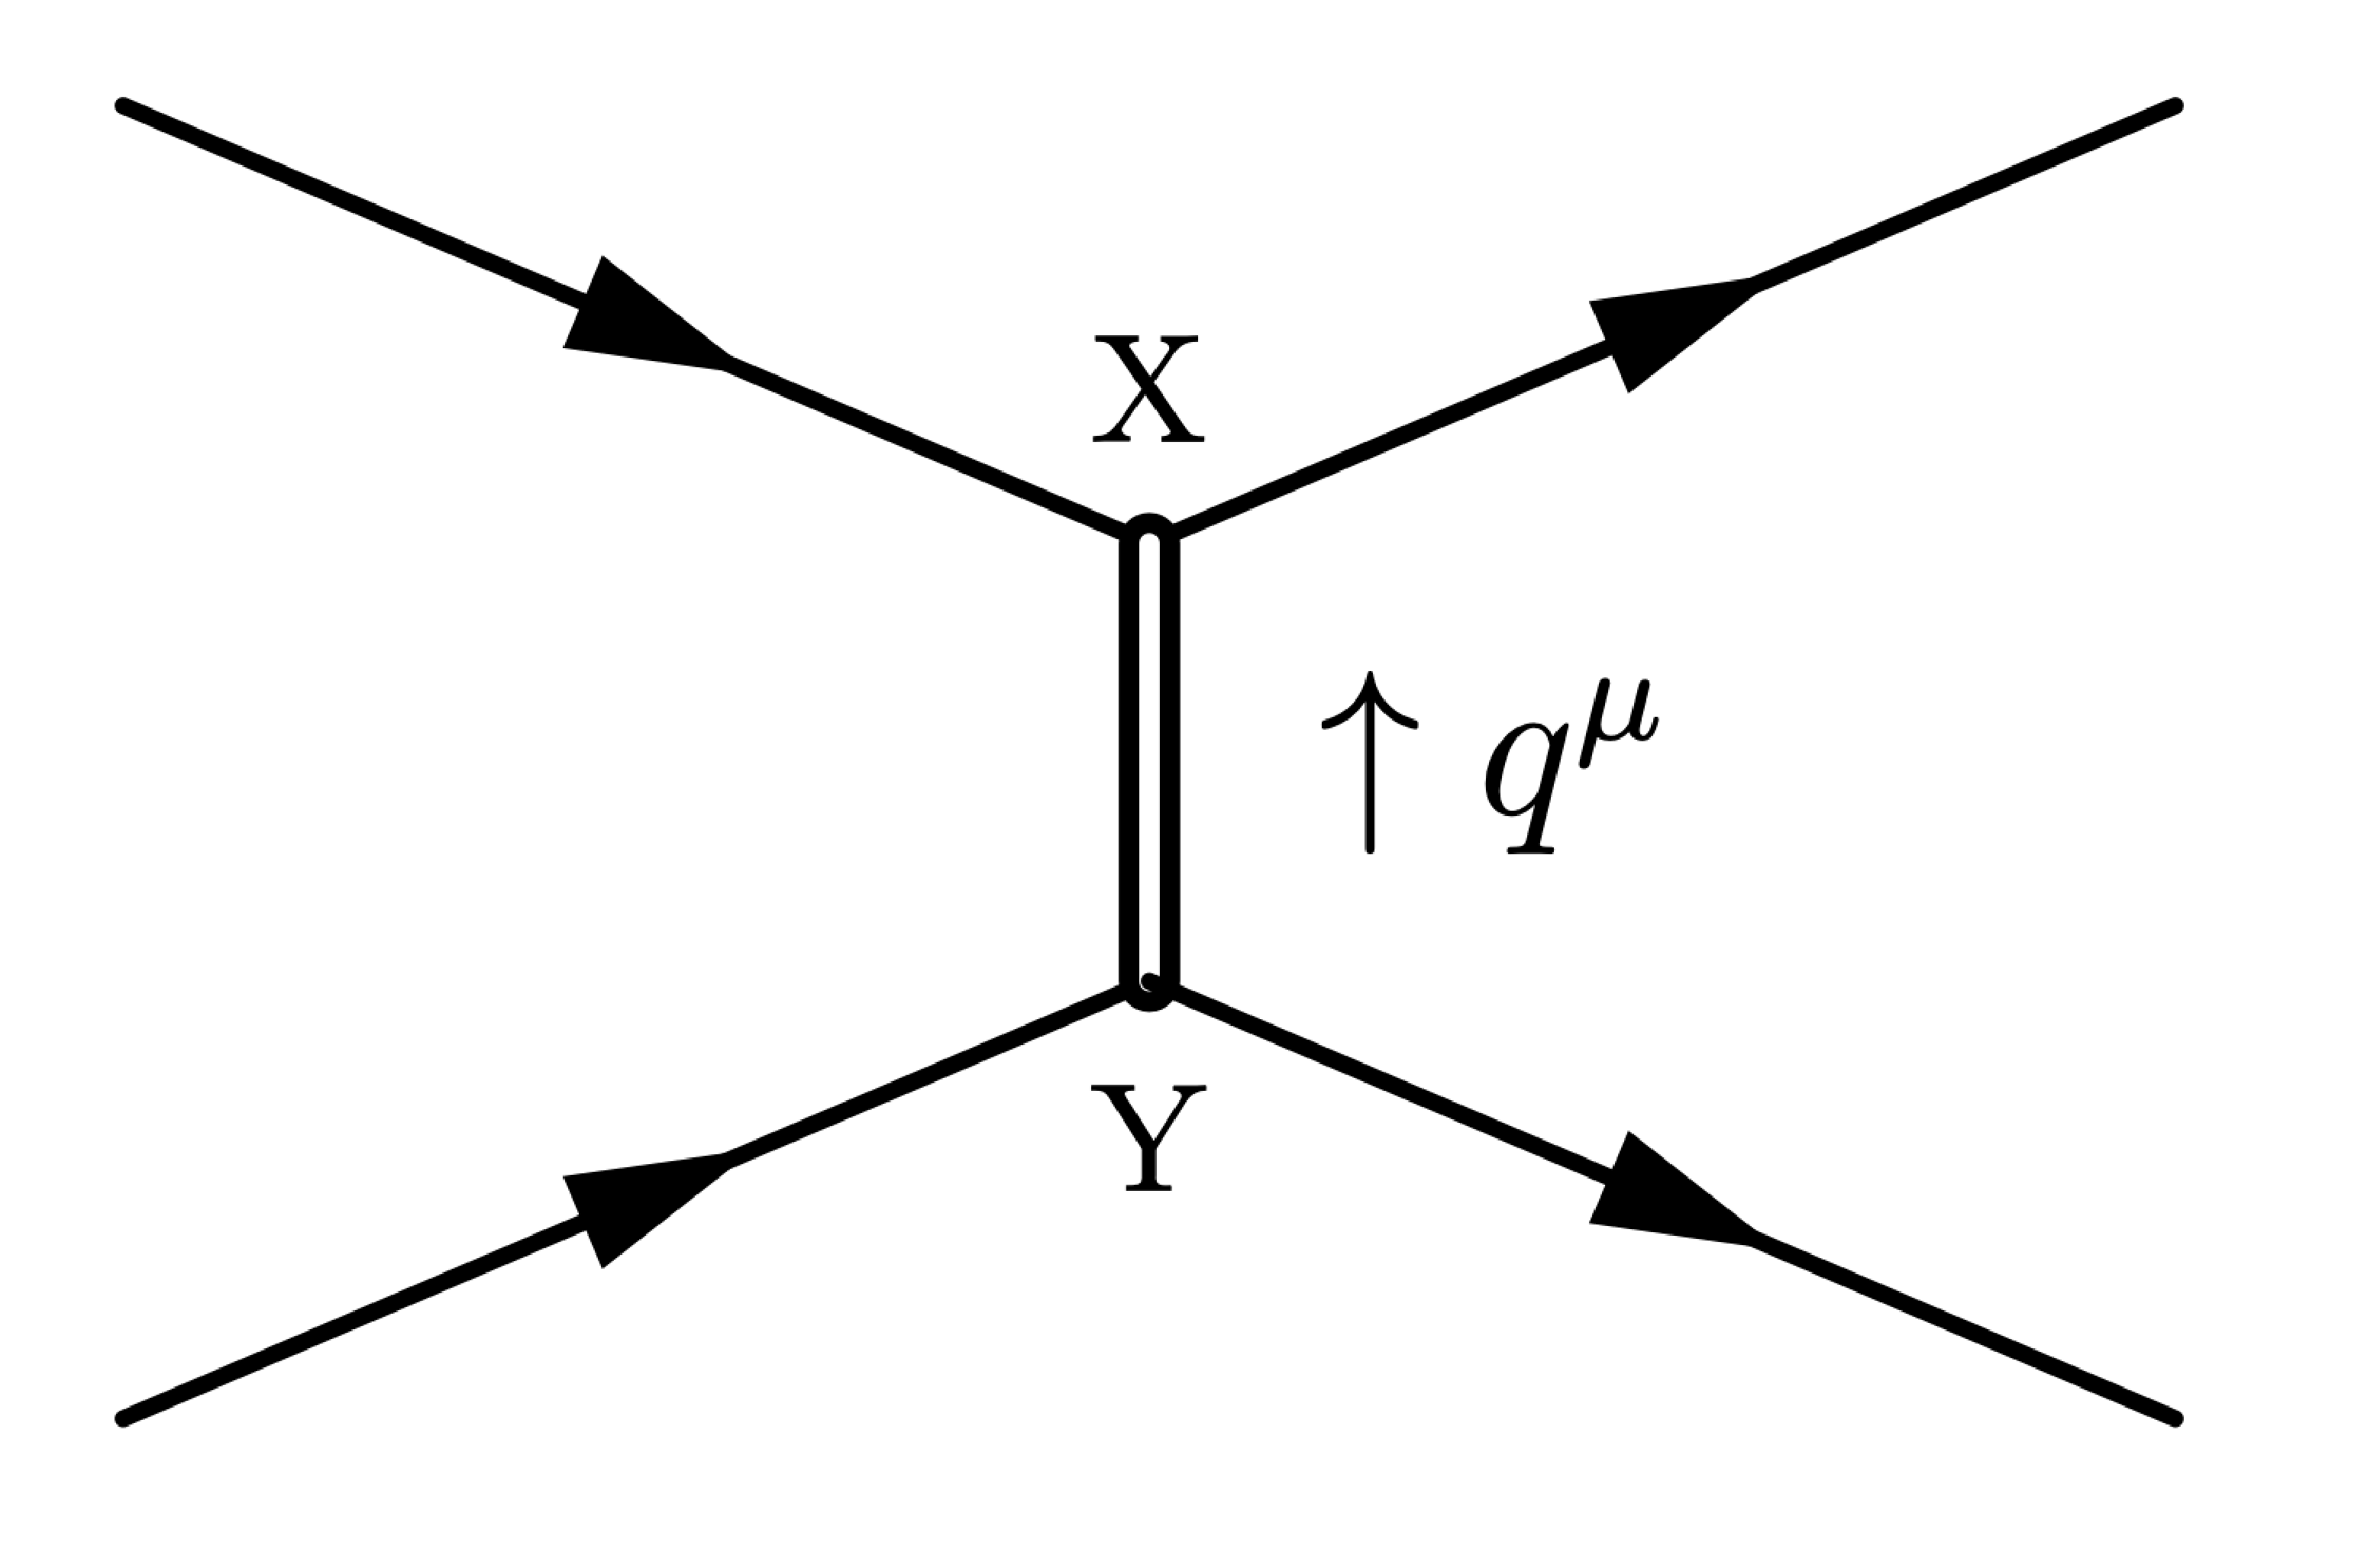
\includegraphics[width=0.27\textwidth]{Fig3.eps}
\caption{Elastic scattering of two fermions with masses $m_X$ and $m_Y$ and spins $\v{s}_X$ and $\v{s}_Y^{\,\prime}$, respectively, mediated by the exchange of a boson of mass $M$ with four-momentum $q^{\mu} = (q^0,\v{q})$ that is transferred from fermion $Y$ to fermion $X$. 
} 
\label{fig:ES}
\end{figure}

We present these potentials below (in the natural units $\hbar=c=1$), 
%\LC{I mention this repeatly because in some later section we are going to put back $\hbar$ and $c$.} 
grouping together interactions with similar features and identifying the dominant terms in the case of\\ 
%\YS{I've re-ordered here following the order in our 2019 spin potentials paper}
%(1) scalar/scalar, pseudoscalar/scalar, pseudoscalar/pseudoscalar, 
%(2) vector/vector, axial-vector/vector, axial-vector/axial-vector, 
%(3) tensor/tensor, pseudotensor/tensor, and pseudotensor/pseudotensor interactions, 
(1) axial-vector/vector, axial-vector/axial-vector, vector/vector, \\
(2) tensor/tensor, pseudotensor/tensor, and pseudotensor/pseudotensor interactions, \\
(3) pseudoscalar/scalar, pseudoscalar/pseudoscalar, scalar/scalar, \\
%\YS{
generated by the exchange of a single %\LC{
massive spin-1 boson of mass $M$, massless spin-1 %} 
boson, and massive or massless spin-0 boson, respectively, between fermions $X$ and $Y$ (see Fig.\,\ref{fig:ES}). 
%
%\LC{Note that for massive spin-1 particles, only the vector interaction is considered in this review, see Eq.\,(\ref{pseudovector-vector_potential}-\ref{vector-vector_potential}), but not the tensor interaction. In principle, this tensor interaction (due to anomalous magnetic moment and EDM)  for massive particles could be included. \DB{Why don't we include it?} In addition, massless spin-1 particle can have tensor, see Eq.\,(\ref{tensor-tensor_potential}-\ref{pseudotensor-pseudotensor_potential}) and vector interactions (see Sec.\,\ref{gAgA_massless}).} 
%
%
%, instead of adopting the symmetry-based approach of \cite{dobrescu_spin-dependent_2006}. 
%\YS{The shorthand labels $V_{11 \pm 16}$ and $V_{14 \pm 15}$ used below may, in isolation, suggest that the $V_{11}$ and $V_{16}$ contributions arise at the same order (and likewise for $V_{14}$ and $V_{15}$). Could we use a differentiating notation like, e.g., $V_{11p \pm 16}$ and $V_{14q \pm 15}$? \LC{Ok}
%Also, the parameter $\v{P}^2$ appearing in the definition of $V_{11 \pm 16}$ needs a suitable definition. Maybe we could define $\v{P}^2$ as a quadratic function of the fermion momenta operators $\v{p}_X$ and $\v{p}_Y$? Technically, there may be a slight difference in the definition of $\v{P}^2$ for $V_{11 + 16}$ and $V_{11 - 16}$.} \LC{Why would here be slight difference?}\LC{In Pasha's thesis, $\v{q}$ is the change of momentum between final and initial state. $\v{P}$ is the average momentum of the final and initial state.}
%\YS{I haven't explicitly checked the form of $\v{P}^2$, but just quickly comparing Eqs.~(\ref{DM_eqV16}) and (\ref{pseudovector-vector_potential}), it seems like the $\v{P}^2$ term in $V_{11+16}|_{AV}$ is related to the $\v{P}^2$ term in $V_{11-16}|_{AV}$ by a permutation like $\v{p}_X \to \v{p}_Y$ (up to a possible sign). \LCa{Yes, you are right.}
%Maybe I should clarify my previous comment above: We don't strictly need to know/present the explicit form of $\v{P}^2$, but we do need to give some description/explanation of what it is. 
%Unless we're sure that $\v{P}^2$ is precisely the average centre-of-mass momentum, my suggestion is to make a more conservation statement like that $\v{P}^2$ is a quadratic function of $\v{p}_X$ and $\v{p}_Y$ (we could in principle rename $\v{P}^2$ as $\v{p}^2$ to avoid potentially confusing it with the centre-of-mass momentum). The most important result for readers remains the full form of the potential in Eq.~(\ref{pseudovector-vector_potential}).} \LCa{I think when speaking of $\v{P}^2$ (and $\v{q}^2$ in $V_{14q+15}$), we are return to the momentum space representation. \citet{dobrescu_spin-dependent_2006} has calculated this in Eq. A.2. Perhaps using $\v{P}^2$ instead of $\v{p}^2$ is more consistent with the derivation there and \cite{fadeev_neue_2018}. What do you think?} 
%\YS{In the case of $\v{P}^2$, I don't think it necessarily matters which representation we take (for consistency with the $\v{q}^2$ case, we could assume the momentum space representation). In Dobrescu's paper, $\v{P}$ is defined as the average momentum of the first fermion (what we would call $\v{p}_X$ in our notation). In addition to this, Dobrescu also considers the centre-of-mass frame (such that $\v{p}_Y = -\v{p}_X$), which we don't assume in our set of equations for the potentials. For this reason, I would avoid using the notation $\v{P}$, which may incorrectly suggest that our notation/formula is only for the centre-of-mass frame.} \LC{Ok}
%\YS{The potentials in Eqs.~(\ref{scalar-pseudoscalar_potential}), (\ref{pseudovector-vector_potential}), and (\ref{pseudotensor-tensor_potential}) are written in an abbreviated form lacking symmetry under the permutation of particle indices $X \leftrightarrow Y$.  In the case of these potentials, we must further add the terms obtained by permuting the particle indices $X \leftrightarrow Y$.} \LC{We have made the changes and mentioned this in the paragraph above.}
%instead of going through all of the 16 individual interactions of \cite{dobrescu_spin-dependent_2006} one by one, as shown below (in the units $\hbar=c=1$): 
%\YS{(Note for self): Need to double-check all formulae and the order in which they appear.}
%\LC{The equations below are copied from the .tex file of \cite{fadeev_revisiting_2019} from arXiv. $\sV_{4+5}$ in Eq.\,\eqref{scalar-scalar_potential} is newly added. $m_{1/2}$ is changed to $m_{X/Y}$ adapt to the format of this review.}
%\YS{I would propose to change the order of the presented potentials to match the order used in our 2019 spin potentials paper (i.e., $ss$, $ps$, $pp$, $VV$, $AV$, $AA$, $TT$, $\tilde{T}T$, $\tilde{T}\tilde{T}$). Some equations below had the original particle index labels $(1,2)$ instead of $(X,Y)$ - I've updated to $(X,Y)$ notation for consistency. \LC{Change the order will need to change the content in the result section, we will consider this when polishing the content there. }
%I've added the $\mathcal{V}_{4+5}$ term to the vector/vector potential. 
%In the case of the scalar/scalar potential, it looks like we currently use a form of $\mathcal{V}_{4+5}$ that is similar to Dobrescu's C.M. approach --- we don't do this in our other equations. 
%I've added an alternate expression/form for $\mathcal{V}_{4+5}$ in red based on how we calculated the other potentials. \LC{OK}
%Pasha, could you please check the expressions for $\mathcal{V}_{4+5}$ for both the vector/vector and scalar/scalar potentials, assuming the approach in our 2019 spin potentials paper? 
%In the equation for $V_{\tilde{T}T}$ below, I think the $m_Y$ in the denominator of the $\mathcal{V}_{9,10}$ term should be $m_Y^2$ (marked in red) - please check. \LC{Corrected.}
%} 
%\LCa{Problem in this paragraph solved.}
%\YS{I've also added the $\mathcal{V}_{4+5}$-type term and $\mathcal{V}_8$ term to the axial-vector/axial-vector potential (marked in red). 
%The $\mathcal{V}_{4+5}$-type term I find is strictly not the same type as for the vector-vector and scalar-scalar cases. 
%In the vector and scalar cases, the spin-momentum correlation involves the same particle. \LC{Yes, I see the difference, in this case, there may be some problem when plotting the limits from $\mathcal{V}'_{4+5}$ for $g_Ag_A$. I will check and shall consider this in the result section. }
%On the other hand, in the pseudovector case, the spin-momentum correlation involves both particles (one particle index for spin and another particle index for momentum). 
%I've hence labelled the $A-A$ contribution by $\mathcal{V}'_{4+5}$ in Eq.~(\ref{pseudovector-pseudovector_potential}) to distinguish from the scalar and vector cases. 
%Pasha, could you please check these results?} 
%\LCa{Here is the refined version of the equations (the planned final format):}
\begin{widetext}
\begin{align}
\label{pseudovector-vector_potential}
\centering
V_{AV}(\v{r}) &= \underbrace{g^X_A g^Y_V \v{\sigma}_X \cdot \left\{ \frac{ \v{p}_X}{m_X} - \frac{ \v{p}_Y}{m_Y} , \frac{e^{-M r}}{ 8 \pi r} \right\} }_{V_{12+13}} +  \underbrace{g^X_V g^Y_A \v\sigma_Y^{\,\prime} \cdot \left\{ \frac{ \v{p}_Y}{m_Y} - \frac{ \v{p}_X}{m_X} , \frac{e^{-M r}}{ 8 \pi r} \right\} }_{V_{12-13}}  \nonumber \\
&\underbrace{ -\frac{g^X_A g^Y_V}{2}  \left(\v{\sigma}_X \times \v\sigma_Y^{\,\prime} \right) \cdot \hat{\v{r}}  \left( \frac{1}{r^2} + \frac{M}{r} \right)  \frac{e^{-M r}}{4 \pi m_Y} }_{V_{11}|_{AV}} \, +\underbrace{ \frac{g^X_Vg^Y_A }{2}  \left(\v\sigma_Y^{\,\prime} \times \v{\sigma }_X \right) \cdot \hat{\v{r}}  \left( \frac{1}{r^2} + \frac{M}{r} \right)  \frac{e^{-M r}}{4 \pi m_X} }_{V_{11}|_{VA}} \nonumber \\
& \underbrace{ - \frac{g_A^X g_V^Y}{4}  \left\{ \boldsymbol{\sigma}_X \cdot \boldsymbol{p}_X , \left\{ \v\sigma_Y^{\,\prime} \cdot \left[ \left( \frac{\v{p}_X}{m_X} - \frac{\v{p}_Y}{m_Y} \right) \times \hat{\v{r}} \right] , \left( \frac{1}{r^2} + \frac{M}{r} \right) \frac{e^{-M r}}{16 \pi m_X m_Y} \right\} \right\}}_{V_{11p+16}|_{AV} \sim \v{p}^2\sV_{11}+\sV_{16}} \nonumber \\
&  \underbrace{ - \frac{g_V^X g_A^Y}{4}  \left\{ \v\sigma_Y^{\,\prime} \cdot \boldsymbol{p}_Y , \left\{ \boldsymbol{\sigma}_X \cdot \left[ \left( \frac{\v{p}_X}{m_X} - \frac{\v{p}_Y}{m_Y} \right) \times \hat{\v{r}} \right] , \left( \frac{1}{r^2} + \frac{M}{r} \right) \frac{e^{-M r}}{16 \pi m_X m_Y} \right\} \right\}}_{V_{11p-16}|_{AV} \sim \v{p}^2\sV_{11}-\sV_{16}} \,,
\end{align}
%%%%%%
\begin{align}
\label{pseudovector-pseudovector_potential}
\centering
&V_{AA}(\v{r}) = \notag\\
&\underbrace{- g^X_A g^Y_A  \v{\sigma}_X \cdot \v\sigma_Y^{\,\prime} \frac{e^{-M r}}{4 \pi r} }_{V_2} \notag \\
&\underbrace{ - \frac{g_A^X g_A^Y m_X m_Y}{ M^2} \left[ \v{\sigma}_X \cdot \v\sigma_Y^{\,\prime} \left[ \frac{1}{r^3} + \frac{M}{r^2} + \frac{4 \pi}{3} \delta(\v{r}) \right]  -  \left( \v{\sigma}_X \cdot \hat{\v{r}} \right) \left( \v\sigma_Y^{\,\prime} \cdot \hat{\v{r}} \right)  \left( \frac{3}{r^3} + \frac{3M}{r^2} + \frac{M^2}{r} \right)  \right] \frac{e^{-M r}}{4 \pi m_X m_Y} }_{V_3|_{AA}} 
\notag \\
&\underbrace{ - \frac{g_A^X g_A^Y}{4} \left\{ \boldsymbol{\sigma}_X \cdot \left( \frac{\boldsymbol{p}_Y}{m_Y^2} \times \hat{\boldsymbol{r}} \right), \left( \frac{1}{r^2} + \frac{M}{r} \right) \frac{e^{-Mr}}{8 \pi} \right\} }_{V_{4+5}|_{AA}} 
+ \underbrace{  \frac{g_A^X g_A^Y}{4} \left\{  \v\sigma_Y^{\,\prime} \cdot \left( \frac{\boldsymbol{p}_X}{m_X^2} \times \hat{\boldsymbol{r}} \right) , \left( \frac{1}{r^2} + \frac{M}{r} \right) \frac{e^{-Mr}}{8 \pi} \right\} }_{V_{4-5}|_{AA}}  \, \nonumber\\
& + \underbrace{g_A^X g_A^Y  \left[ \left\{ \frac{\boldsymbol{\sigma}_X \cdot \boldsymbol{p}_X}{m_X} , \left\{ \frac{\v\sigma_Y^{\,\prime} \cdot \boldsymbol{p}_Y}{m_Y} , \frac{e^{-M r}}{16 \pi r} \right\} \right\} - \frac{1}{2}\left\{ \frac{\boldsymbol{\sigma}_X \cdot \boldsymbol{p}_Y}{m_Y} , \left\{ \frac{\v\sigma_Y^{\,\prime} \cdot \boldsymbol{p}_Y}{m_Y} , \frac{e^{-M r}}{16 \pi r} \right\} \right\} -\frac{1}{2}\left\{ \frac{\boldsymbol{\sigma}_X \cdot \boldsymbol{p}_X}{m_X} , \left\{ \frac{\v\sigma_Y^{\,\prime} \cdot \boldsymbol{p}_X}{m_X} , \frac{e^{-M r}}{16 \pi r} \right\} \right\} \right] }_{V_8}\,,
\end{align}
%%%%%%
\begin{align}
\label{vector-vector_potential}
&V_{VV}(\v{r})= \notag\\
& \underbrace{g^X_V g^Y_V \frac{e^{-M r}}{4 \pi r} }_{V_1|_{VV}}
+  \underbrace{\frac{g^X_V g^Y_V }{4}  \left[ \v{\sigma}_X \cdot \v\sigma_Y^{\,\prime} \left[ \frac{1}{r^3} + \frac{M}{r^2} + \frac{M^2}{r} - \frac{8 \pi}{3} \delta(\v{r}) \right]  -  \left( \v{\sigma}_X \cdot \hat{\v{r}} \right) \left( \v\sigma_Y^{\,\prime}\cdot \hat{\v{r}} \right)  \left[ \frac{3}{r^3} + \frac{3M}{r^2} + \frac{M^2}{r} \right]  \right] \frac{e^{-M r}}{4 \pi m_X m_Y} }_{(V_2 + V_3)|_{VV}} \notag \\
 & + \underbrace{ \frac{g_V^X g_V^Y}{4} \left\{ \boldsymbol{\sigma}_X \cdot \left( \frac{\boldsymbol{p}_X}{m_X^2} \times \hat{\boldsymbol{r}} \right) 
 - 2 \boldsymbol{\sigma}_X \cdot \left( \frac{\boldsymbol{p}_Y}{m_X m_Y} \times \hat{\boldsymbol{r}} \right)
, \left( \frac{1}{r^2} + \frac{M}{r} \right) \frac{e^{-Mr}}{8 \pi} \right\} }_{V_{4+5}|_{VV}}\notag\\
  & \underbrace{- \frac{g_V^X g_V^Y}{4} \left\{
  \v\sigma_Y^{\,\prime} \cdot \left( \frac{\boldsymbol{p}_Y}{m_Y^2} \times \hat{\boldsymbol{r}} \right) 
 - 2 \v\sigma_Y^{\,\prime} \cdot \left( \frac{\boldsymbol{p}_X}{m_X m_Y} \times \hat{\boldsymbol{r}} \right)
 , \left( \frac{1}{r^2} + \frac{M}{r} \right) \frac{e^{-Mr}}{8 \pi} \right\} }_{V_{4-5}|_{VV}} \, ,
\end{align}
%%%%%%
and
\begin{equation}
\label{tensor-tensor_potential}
V_{TT}(\v{r}) =  \underbrace{\frac{4 v_h^2 \mathrm{Re}(C_X) \mathrm{Re}(C_Y) m_X m_Y}{\Lambda^4 } 
 \left[  \v{\sigma}_X \cdot \v\sigma_Y^{\,\prime} \left[ \frac{1}{r^3} - \frac{8 \pi}{3} \delta(\v{r}) \right]  - \left( \v{\sigma}_X \cdot \hat{\v{r}} \right) \left( \v\sigma_Y^{\,\prime}\cdot \hat{\v{r}} \right)  \frac{3}{r^3}  \right] \frac{1}{4 \pi m_X m_Y}  }_{(V_2 + V_3)|_{TT}} \, ,
\end{equation}

%\LC{We may want to check if we can simplify the below $V_{14\pm15}|_{\tilde{T}T}$ a little bit.  } 
%\YS{The updated equations look good to me. We can add an explanation in the text that summation over the index $i=1,2,3$ is implied.} 
{\small
\begin{align}
\label{pseudotensor-tensor_potential}
&V_{\tilde{T}T}(\v{r}) = \notag\\
 &\underbrace{ \frac{4 v_h^2 \mathrm{Im}(C_X) \mathrm{Re}(C_Y) m_X m_Y }{ \Lambda^4 }  \left[ \left(\v{\sigma}_X \times \v\sigma_Y^{\,\prime} \right) \cdot \left\{ \frac{\v{p}_X}{m_X} - \frac{\v{p}_Y}{m_Y}  , ~ 
 \frac{1}{r^3} + \frac{4 \pi}{3} \delta(\v{r}) \right\}+  \left\{   \left( \frac{\v{p}_X}{m_X} - \frac{\v{p}_Y}{m_Y} \right)_i  , ~ \frac{3 \left(\v{\sigma}_X \cdot \hat{\v{r}} \right) \left(\v\sigma_Y^{\,\prime} \times \hat{\v{r}} \right)_i }{r^3} \right\} \right] \frac{1}{8 \pi m_X m_Y} }_{  V_{14q+15}|_{\tilde{T}T}  } \notag\\
 + &\underbrace{  \frac{4 v_h^2 \mathrm{Im}(C_Y) \mathrm{Re}(C_X) m_X m_Y }{ \Lambda^4 } \left[ \left(\v\sigma_Y^{\,\prime} \times \v{\sigma}_X \right) \cdot \left\{ \frac{\v{p}_Y}{m_Y} - \frac{\v{p}_X}{m_X}  , ~ 
 \frac{1}{r^3} + \frac{4 \pi}{3} \delta(\v{r}) \right\}+  \left\{   \left( \frac{\v{p}_Y}{m_Y} - \frac{\v{p}_X}{m_X} \right)_i  , ~ \frac{3 \left(\v\sigma_Y^{\,\prime} \cdot \hat{\v{r}} \right) \left(\v{\sigma}_X \times \hat{\v{r}} \right)_i }{r^3} \right\} \right] \frac{1}{8 \pi m_X m_Y} }_{ V_{14q-15}|_{\tilde{T}T}   }\notag \\
&\underbrace{-\frac{2 v_h^2 \mathrm{Im}(C_X) \mathrm{Re}(C_Y) m_X m_Y }{\Lambda^4} \frac{\v{\sigma}_X \cdot [\v{\nabla} \delta(\v{r})] }{ m_X m_Y^2 }  }_{ V_{9+10}|_{\tilde{T}T}  } +\underbrace{\frac{2 v_h^2 \mathrm{Im}(C_Y) \mathrm{Re}(C_X) m_X m_Y }{\Lambda^4} \frac{\v\sigma_Y^{\,\prime} \cdot [\v{\nabla} \delta(\v{r})] }{ m_Ym_X^2}  }_{ V_{9-10}|_{\tilde{T}T}  } \, , 
\end{align}
}
%%%%%%
\begin{equation}
\label{pseudotensor-pseudotensor_potential}
V_{\tilde{T}\tilde{T}}(\v{r}) =  \underbrace{ \frac{4 v_h^2 \mathrm{Im}(C_X) \mathrm{Im}(C_Y) m_X m_Y}{\Lambda^4 } 
 \left[  \v{\sigma}_X \cdot \v\sigma_Y^{\,\prime}\left[ \frac{1}{r^3} + \frac{4 \pi}{3} \delta(\v{r}) \right]  -  \left( \v{\sigma}_X \cdot \hat{\v{r}} \right) \left( \v\sigma_Y^{\,\prime}\cdot \hat{\v{r}} \right)   \frac{3}{r^3}  \right]  \frac{1}{4 \pi m_X m_Y}  }_{V_3|_{\tilde{T}\tilde{T}}} \, . 
\end{equation}
%%%
and
\begin{align}
\label{scalar-pseudoscalar_potential}
&V_{ps}(\v{r})= \notag\\
&\underbrace{ - g^X_p g^Y_s \v{\sigma}_X \cdot \hat{\v{r}} \left( \frac{1}{r^2} + \frac{M}{r} \right) \frac{e^{-M r}}{8 \pi m_X} }_{V_{9+10}|_{ps}}   
+ \underbrace{g^Y_p g^X_s  \v\sigma_Y^{\,\prime} \cdot \hat{\v{r}} \left( \frac{1}{r^2} + \frac{M}{r} \right) \frac{e^{-M r}}{8 \pi m_Y} }_{V_{9-10}|_{ps}} \notag \\
& + \underbrace{\frac{g^X_p g^Y_s}{8} \left[ \left\{ \left( \v{\sigma}_X \times \v\sigma_Y^{\,\prime} \right) \cdot \frac{\v{p}_Y}{m_Y} , \frac{1}{r^3} + \frac{M}{r^2} + \frac{4 \pi}{3} \delta(\v{r})  \right\} -\left\{ \left( \v{\sigma}_X \cdot \hat{\v{r}} \right) \v\sigma_Y^{\,\prime} \cdot \left( \frac{\v{p}_Y}{m_Y} \times \hat{\v{r}} \right) , \frac{3}{r^3} + \frac{3M}{r^2} + \frac{M^2}{r}  \right\}\right]\frac{e^{-M r}}{8 \pi m_X m_Y}  }_{V_{14q+15}|_{ps}\sim \v{q}^2\sV_{14}+\sV_{15}}  \notag\\
&+ \underbrace{\frac{g^Y_p g^X_s}{8} \left[\left\{ \left( \v\sigma_Y^{\,\prime} \times \v{\sigma}_X \right) \cdot \frac{\v{p}_X}{m_X} , \frac{1}{r^3} + \frac{M}{r^2} + \frac{4 \pi}{3} \delta(\v{r}) \right\} -\left\{ \left( \v\sigma_Y^{\,\prime} \cdot \hat{\v{r}} \right) \v{\sigma}_X \cdot \left( \frac{\v{p}_X}{m_X} \times \hat{\v{r}} \right) , \frac{3}{r^3} + \frac{3M}{r^2} + \frac{M^2}{r} \right\} \right]\frac{e^{-M r}}{8 \pi m_X m_Y} }_{V_{14q-15}|_{ps}\sim\v{q}^2\sV_{14}-\sV_{15}} \, ,
\end{align}
%%%%%%
\begin{equation}
\label{pseudoscalar-pseudoscalar_potential}
V_{pp}(\v{r}) = \underbrace{ -  \frac{g^X_p g^Y_p}{4}  \left[  \v{\sigma}_X \cdot \v\sigma_Y^{\,\prime}\left[ \frac{1}{r^3} + \frac{M}{r^2} + \frac{4 \pi}{3} \delta(\v{r}) \right]
- \left( \v{\sigma}_X \cdot \hat{\v{r}} \right) \left( \v\sigma_Y^{\,\prime}\cdot \hat{\v{r}} \right)  \left[ \frac{3}{r^3} + \frac{3M}{r^2} + \frac{M^2}{r} \right]   \right] \frac{e^{-M r}}{4 \pi m_X m_Y} }_{V_3|_{pp}} \, ,
\end{equation}
%%%%%%
\begin{align}
\label{scalar-scalar_potential}
V_{ss}(\v{r}) = \underbrace{  -  g^X_s g^Y_s \frac{e^{-M r}}{ 4 \pi r} }_{V_1|_{ss}} 
+ \underbrace{ \frac{g_s^X g_s^Y}{4} \left\{ \boldsymbol{\sigma}_X \cdot \left( \frac{\boldsymbol{p}_X}{m_X^2} \times \hat{\boldsymbol{r}} \right), \left( \frac{1}{r^2} + \frac{M}{r} \right) \frac{e^{-Mr}}{8 \pi} \right\} }_{V_{4+5}|_{ss}} - 
\underbrace{ \frac{g_s^X g_s^Y}{4} \left\{ \v\sigma_Y^{\,\prime} \cdot \left( \frac{\boldsymbol{p}_Y}{m_Y^2} \times \hat{\boldsymbol{r}} \right) , \left( \frac{1}{r^2} + \frac{M}{r} \right) \frac{e^{-Mr}}{8 \pi} \right\} }_{V_{4-5}|_{ss}}\, , 
\end{align}
%%%%%%
\end{widetext}
%\LC{Below are equations with our change records (Shall be deleted after we confirm the final format} \LCa{I have hide them now.}
\iffalse
\begin{widetext}
\begin{align}
\label{pseudovector-vector_potential}
V_{AV}(\v{r}) &= \LCa{ \underbrace{g^X_A g^Y_V \v{\sigma}_X \cdot \left\{ \frac{ \v{p}_X}{m_X} - \frac{ \v{p}_Y}{m_Y} , \frac{e^{-M r}}{ 8 \pi r} \right\} }_{V_{12+13}} +  \underbrace{g^X_V g^Y_A \v\sigma_Y^{\,\prime}\cdot \left\{ \frac{ \v{p}_Y}{m_Y} - \frac{ \v{p}_X}{m_X} , \frac{e^{-M r}}{ 8 \pi r} \right\} }_{V_{12-13}}  }\nonumber \\
&\underbrace{ -\frac{g^X_A g^Y_V}{2}  \left(\v{\sigma}_X \times \v\sigma_Y^{\,\prime}\right) \cdot \hat{\v{r}}  \left( \frac{1}{r^2} + \frac{M}{r} \right)  \frac{e^{-M r}}{4 \pi m_Y} }_{V_{11}|_{AV}} \, \LC{+\underbrace{ \frac{g^X_Vg^Y_A }{2}  \left(\v\sigma_Y^{\,\prime}\times \v{\sigma }_X \right) \cdot \hat{\v{r}}  \left( \frac{1}{r^2} + \frac{M}{r} \right)  \frac{e^{-M r}}{4 \pi m_X} }_{V_{11}|_{VA}} \, }\\
%&\LCa{\underbrace{-{g^X_A g^Y_V}  \left[ \left(\v{\sigma}_X \times \v\sigma_Y^{\,\prime}\right) \cdot \hat{\v{r}}  \, -  \left(\v{\sigma}_Y \times \v{\sigma }_X \right) \cdot \hat{\v{r}}  \right] \left( \frac{1}{r^2} + \frac{M}{r} \right)  \frac{e^{-M r}}{8 \pi m_X} }_{\mathcal{V}_{11}} }
\nonumber\,,
\end{align}
%%%%%%
\begin{align}
\label{pseudovector-pseudovector_potential}
V_{AA}(\v{r}) &=  - g^X_A g^Y_A \underbrace{ \v{\sigma}_X \cdot \v\sigma_Y^{\,\prime}\frac{e^{-M r}}{4 \pi r} }_{\mathcal{V}_2} 
- \frac{g_A^X g_A^Y m_X m_Y}{ M^2} \underbrace{ \left[ \v{\sigma}_X \cdot \v\sigma_Y^{\,\prime}\left[ \frac{1}{r^3} + \frac{M}{r^2} + \frac{4 \pi}{3} \delta(\v{r}) \right]  -  \left( \v{\sigma}_X \cdot \hat{\v{r}} \right) \left( \v\sigma_Y^{\,\prime}\cdot \hat{\v{r}} \right)  \left( \frac{3}{r^3} + \frac{3M}{r^2} + \frac{M^2}{r} \right)  \right] \frac{e^{-M r}}{4 \pi m_X m_Y} }_{\mathcal{V}_3} 
\notag \\
&{\color{red} - \frac{g_A^X g_A^Y}{4} \underbrace{ \left\{ \boldsymbol{\sigma}_X \cdot \left( \frac{\boldsymbol{p}_Y}{m_Y^2} \times \hat{\boldsymbol{r}} \right) - \v\sigma_Y^{\,\prime} \cdot \left( \frac{\boldsymbol{p}_X}{m_X^2} \times \hat{\boldsymbol{r}} \right) , \left( \frac{1}{r^2} + \frac{M}{r} \right) \frac{e^{-Mr}}{8 \pi} \right\} }_{\mathcal{V}'_{4,5}}} \nonumber \\
&{\color{red} + g_A^X g_A^Y \underbrace{ \left[ \left\{ \frac{\boldsymbol{\sigma}_X \cdot \boldsymbol{p}_X}{m_X} , \left\{ \frac{\v\sigma_Y^{\,\prime} \cdot \boldsymbol{p}_Y}{m_Y} , \frac{e^{-M r}}{16 \pi r} \right\} \right\} - \frac{1}{2}\left\{ \frac{\boldsymbol{\sigma}_X \cdot \boldsymbol{p}_Y}{m_Y} , \left\{ \frac{\v\sigma_Y^{\,\prime} \cdot \boldsymbol{p}_Y}{m_Y} , \frac{e^{-M r}}{16 \pi r} \right\} \right\} -\frac{1}{2}\left\{ \frac{\boldsymbol{\sigma}_X \cdot \boldsymbol{p}_X}{m_X} , \left\{ \frac{\v\sigma_Y^{\,\prime} \cdot \boldsymbol{p}_X}{m_X} , \frac{e^{-M r}}{16 \pi r} \right\} \right\} \right] }_{\mathcal{V}_8}}\, , \nonumber \\
&\LCa{ \underbrace{ - \frac{g_A^X g_A^Y}{4} \left\{ \boldsymbol{\sigma}_X \cdot \left( \frac{\boldsymbol{p}_Y}{m_Y^2} \times \hat{\boldsymbol{r}} \right), \left( \frac{1}{r^2} + \frac{M}{r} \right) \frac{e^{-Mr}}{8 \pi} \right\} }_{\mathcal{V}_{4+5}|_{AA}}} 
+\LCa{ \underbrace{  \frac{g_A^X g_A^Y}{4} \left\{  \v\sigma_Y^{\,\prime} \cdot \left( \frac{\boldsymbol{p}_X}{m_X^2} \times \hat{\boldsymbol{r}} \right) , \left( \frac{1}{r^2} + \frac{M}{r} \right) \frac{e^{-Mr}}{8 \pi} \right\} }_{\mathcal{V}_{4-5}|_{AA}}}  \, ,
\end{align}
%%%%%%
\begin{align}
\label{vector-vector_potential}
V_{VV}(\v{r}) &= g^X_V g^Y_V \underbrace{ \frac{e^{-M r}}{4 \pi r} }_{\mathcal{V}_1}
+  \frac{g^X_V g^Y_V }{4} \underbrace{ \left[ \v{\sigma}_X \cdot \v\sigma_Y^{\,\prime} \left[ \frac{1}{r^3} + \frac{M}{r^2} + \frac{M^2}{r} - \frac{8 \pi}{3} \delta(\v{r}) \right]  -  \left( \v{\sigma}_X \cdot \hat{\v{r}} \right) \left( \v\sigma_Y^{\,\prime}\cdot \hat{\v{r}} \right)  \left[ \frac{3}{r^3} + \frac{3M}{r^2} + \frac{M^2}{r} \right]  \right] \frac{e^{-M r}}{4 \pi m_X m_Y} }_{\mathcal{V}_2 + \mathcal{V}_3} \notag \\
 & {\color{red} + \frac{g_V^X g_V^Y}{4} \underbrace{ \left\{ \boldsymbol{\sigma}_X \cdot \left( \frac{\boldsymbol{p}_X}{m_X^2} \times \hat{\boldsymbol{r}} \right) 
 - 2 \boldsymbol{\sigma}_X \cdot \left( \frac{\boldsymbol{p}_Y}{m_X m_Y} \times \hat{\boldsymbol{r}} \right)
 - \v\sigma_Y^{\,\prime} \cdot \left( \frac{\boldsymbol{p}_Y}{m_Y^2} \times \hat{\boldsymbol{r}} \right) 
 + 2 \v\sigma_Y^{\,\prime} \cdot \left( \frac{\boldsymbol{p}_X}{m_X m_Y} \times \hat{\boldsymbol{r}} \right)
 , \left( \frac{1}{r^2} + \frac{M}{r} \right) \frac{e^{-Mr}}{8 \pi} \right\} }_{\mathcal{V}_{4,5}}}\notag \\
 & \LCa{ + \underbrace{ \frac{g_V^X g_V^Y}{4} \left\{ \boldsymbol{\sigma}_X \cdot \left( \frac{\boldsymbol{p}_X}{m_X^2} \times \hat{\boldsymbol{r}} \right) 
 - 2 \boldsymbol{\sigma}_X \cdot \left( \frac{\boldsymbol{p}_Y}{m_X m_Y} \times \hat{\boldsymbol{r}} \right)
, \left( \frac{1}{r^2} + \frac{M}{r} \right) \frac{e^{-Mr}}{8 \pi} \right\} }_{\mathcal{V}_{4+5}|_{VV}}}\notag\\
  &+\LCa{ - \underbrace{ \frac{g_V^X g_V^Y}{4} \left\{
  \v\sigma_Y^{\,\prime} \cdot \left( \frac{\boldsymbol{p}_Y}{m_Y^2} \times \hat{\boldsymbol{r}} \right) 
 - 2 \v\sigma_Y^{\,\prime} \cdot \left( \frac{\boldsymbol{p}_X}{m_X m_Y} \times \hat{\boldsymbol{r}} \right)
 , \left( \frac{1}{r^2} + \frac{M}{r} \right) \frac{e^{-Mr}}{8 \pi} \right\} }_{\mathcal{V}_{4-5}|_{VV}}}
\, ,
\end{align}
%%%%%%
and
\begin{align}
\label{scalar-pseudoscalar_potential}
V_{ps}(\v{r}) &= - g^X_p g^Y_s \underbrace{ \v{\sigma}_X \cdot \hat{\v{r}} \left( \frac{1}{r^2} + \frac{M}{r} \right) \frac{e^{-M r}}{8 \pi m_X} }_{\mathcal{V}_{9,10}} \notag \\ 
& \LC{- g^X_p g^Y_s \underbrace{ \v{\sigma}_X \cdot \hat{\v{r}} \left( \frac{1}{r^2} + \frac{M}{r} \right) \frac{e^{-M r}}{8 \pi m_X} }_{\mathcal{V}_{9,10}} + g^Y_p g^X_s \underbrace{ \v\sigma_Y^{\,\prime}\cdot \hat{\v{r}} \left( \frac{1}{r^2} + \frac{M}{r} \right) \frac{e^{-M r}}{8 \pi m_Y} }_{\mathcal{V}_{9,10}}} \notag \\
&\LCa{\underbrace{ - g^X_p g^Y_s \v{\sigma}_X \cdot \hat{\v{r}} \left( \frac{1}{r^2} + \frac{M}{r} \right) \frac{e^{-M r}}{8 \pi m_X} }_{\mathcal{V}_{9+10}}   
+ \underbrace{g^Y_p g^X_s  \v\sigma_Y^{\,\prime}\cdot \hat{\v{r}} \left( \frac{1}{r^2} + \frac{M}{r} \right) \frac{e^{-M r}}{8 \pi m_Y} }_{\mathcal{V}_{9-10}}} \notag \\
& {\color{red} + \frac{g^X_p g^Y_s}{8} \underbrace{ \left\{ \left( \v{\sigma}_X \times \v\sigma_Y^{\,\prime}\right) \cdot \frac{\v{p}_Y}{m_Y} , \left[ \frac{1}{r^3} + \frac{M}{r^2} + \frac{4 \pi}{3} \delta(\v{r}) \right] \frac{e^{-M r}}{8 \pi m_X m_Y} \right\} }_{\mathcal{V}'_{14}} 
+ \frac{g^Y_p g^X_s}{8} \underbrace{ \left\{ \left( \v\sigma_Y^{\,\prime}\times \v{\sigma}_X \right) \cdot \frac{\v{p}_X}{m_X} , \left[ \frac{1}{r^3} + \frac{M}{r^2} + \frac{4 \pi}{3} \delta(\v{r}) \right] \frac{e^{-M r}}{8 \pi m_X m_Y} \right\} }_{\mathcal{V}'_{14}} } \notag \\ 
& {\color{red} - \frac{g^X_p g^Y_s}{8} \underbrace{ \left\{ \left( \v{\sigma}_X \cdot \hat{\v{r}} \right) \v\sigma_Y^{\,\prime}\cdot \left( \frac{\v{p}_Y}{m_Y} \times \hat{\v{r}} \right) , \left[ \frac{3}{r^3} + \frac{3M}{r^2} + \frac{M^2}{r} \right] \frac{e^{-M r}}{8 \pi m_X m_Y} \right\} }_{\mathcal{V}_{15}}
- \frac{g^Y_p g^X_s}{8} \underbrace{ \left\{ \left( \v\sigma_Y^{\,\prime}\cdot \hat{\v{r}} \right) \v{\sigma}_X \cdot \left( \frac{\v{p}_X}{m_X} \times \hat{\v{r}} \right) , \left[ \frac{3}{r^3} + \frac{3M}{r^2} + \frac{M^2}{r} \right] \frac{e^{-M r}}{8 \pi m_X m_Y} \right\} }_{\mathcal{V}_{15}} } \notag \\ 
& \LCa{+ \frac{g^X_p g^Y_s}{8} \underbrace{\left[ \left\{ \left( \v{\sigma}_X \times \v\sigma_Y^{\,\prime}\right) \cdot \frac{\v{p}_Y}{m_Y} , \frac{1}{r^3} + \frac{M}{r^2} + \frac{4 \pi}{3} \delta(\v{r})  \right\} -\left\{ \left( \v{\sigma}_X \cdot \hat{\v{r}} \right) \v\sigma_Y^{\,\prime}\cdot \left( \frac{\v{p}_Y}{m_Y} \times \hat{\v{r}} \right) , \frac{3}{r^3} + \frac{3M}{r^2} + \frac{M^2}{r}  \right\}\right]\frac{e^{-M r}}{8 \pi m_X m_Y}  }_{\mathcal{V}_{14q+15}} } \notag\\
&\LCa{+ \frac{g^Y_p g^X_s}{8} \underbrace{\left[\left\{ \left( \v\sigma_Y^{\,\prime}\times \v{\sigma}_X \right) \cdot \frac{\v{p}_X}{m_X} , \frac{1}{r^3} + \frac{M}{r^2} + \frac{4 \pi}{3} \delta(\v{r}) \right\} -\left\{ \left( \v\sigma_Y^{\,\prime}\cdot \hat{\v{r}} \right) \v{\sigma}_X \cdot \left( \frac{\v{p}_X}{m_X} \times \hat{\v{r}} \right) , \frac{3}{r^3} + \frac{3M}{r^2} + \frac{M^2}{r} \right\} \right]\frac{e^{-M r}}{8 \pi m_X m_Y} }_{\mathcal{V}_{14q-15}} } \\ 
%& \LCa{\underbrace{- \frac{g^X_p g^Y_s}{8} \left\{ \left( \v{\sigma}_X \cdot \hat{\v{r}} \right) \v{\sigma}_Y \cdot \left( \frac{\v{p}_Y}{m_Y} \times \hat{\v{r}} \right) -\left( \v{\sigma}_Y \cdot \hat{\v{r}} \right) \v{\sigma}_X \cdot \left( \frac{\v{p}_X}{m_X} \times \hat{\v{r}} \right) , \left[ \frac{3}{r^3} + \frac{3M}{r^2} + \frac{M^2}{r} \right] \frac{e^{-M r}}{8 \pi m_X m_Y} \right\} }_{\mathcal{V}_{15}} }
\notag\, ,
\end{align}
%%%%%%
\begin{equation}
\label{pseudoscalar-pseudoscalar_potential}
V_{pp}(\v{r}) = -  \frac{g^X_p g^Y_p}{4} \underbrace{ \left[  \v{\sigma}_X \cdot \v\sigma_Y^{\,\prime}\left[ \frac{1}{r^3} + \frac{M}{r^2} + \frac{4 \pi}{3} \delta(\v{r}) \right]
- \left( \v{\sigma}_X \cdot \hat{\v{r}} \right) \left( \v\sigma_Y^{\,\prime}\cdot \hat{\v{r}} \right)  \left[ \frac{3}{r^3} + \frac{3M}{r^2} + \frac{M^2}{r} \right]   \right] \frac{e^{-M r}}{4 \pi m_X m_Y} }_{\mathcal{V}_3} \, ,
\end{equation}
%%%%%%
\begin{align}
\label{scalar-scalar_potential}
V_{ss}(\v{r}) =  -  g^X_s g^Y_s \underbrace{ \frac{e^{-M r}}{ 4 \pi r} }_{\mathcal{V}_1} +g^X_s g^Y_s\underbrace{\boldsymbol{\sigma} \cdot(\boldsymbol{v} \times \hat{\boldsymbol{r}}) (\frac{1}{r^2}+\frac{1}{\lambda r}) \frac{m_Y e^{-M r}}{16\pi m_X(m_X+m_Y)} }_{\sV_{4+5}} \notag \\
{\color{red} + \frac{g_s^X g_s^Y}{4} \underbrace{ \left\{ \boldsymbol{\sigma}_X \cdot \left( \frac{\boldsymbol{p}_X}{m_X^2} \times \hat{\boldsymbol{r}} \right) - \v\sigma_Y^{\,\prime} \cdot \left( \frac{\boldsymbol{p}_Y}{m_Y^2} \times \hat{\boldsymbol{r}} \right) , \left( \frac{1}{r^2} + \frac{M}{r} \right) \frac{e^{-Mr}}{8 \pi} \right\} }_{\mathcal{V}_{4,5}}}\notag \\
\LCa{ + \underbrace{ \frac{g_s^X g_s^Y}{4} \left\{ \boldsymbol{\sigma}_X \cdot \left( \frac{\boldsymbol{p}_X}{m_X^2} \times \hat{\boldsymbol{r}} \right), \left( \frac{1}{r^2} + \frac{M}{r} \right) \frac{e^{-Mr}}{8 \pi} \right\} }_{\mathcal{V}_{4+5}|_{ss}}+
\underbrace{ \frac{g_s^X g_s^Y}{4} \left\{ - \v\sigma_Y^{\,\prime} \cdot \left( \frac{\boldsymbol{p}_Y}{m_Y^2} \times \hat{\boldsymbol{r}} \right) , \left( \frac{1}{r^2} + \frac{M}{r} \right) \frac{e^{-Mr}}{8 \pi} \right\} }_{\mathcal{V}_{4-5}|_{ss}}}
\, , 
\end{align}
%%%%%%
and
\begin{equation}
\label{tensor-tensor_potential}
V_{TT}(\v{r}) =  \frac{4 v_h^2 \mathrm{Re}(C_X) \mathrm{Re}(C_Y) m_X m_Y}{\Lambda^4 } 
\underbrace{ \left[  \v{\sigma}_X \cdot \v\sigma_Y^{\,\prime} \left[ \frac{1}{r^3} - \frac{8 \pi}{3} \delta(\v{r}) \right]  - \left( \v{\sigma}_X \cdot \hat{\v{r}} \right) \left( \v\sigma_Y^{\,\prime}\cdot \hat{\v{r}} \right)  \frac{3}{r^3}  \right] \frac{1}{4 \pi m_X m_Y}  }_{\mathcal{V}_2 + \mathcal{V}_3} \, ,
\end{equation}
%%%%%%
\begin{align}
\label{pseudotensor-tensor_potential}
V_{\tilde{T}T}(\v{r}) = &  \frac{4 v_h^2 \mathrm{Im}(C_X) \mathrm{Re}(C_Y) m_X m_Y }{ \Lambda^4 } \underbrace{ \left[ \left(\v{\sigma}_X \times \v\sigma_Y^{\,\prime}\right) \cdot \left\{ \frac{\v{p}_X}{m_X} - \frac{\v{p}_Y}{m_Y}  , ~ 
 \frac{1}{r^3} + \frac{4 \pi}{3} \delta(\v{r}) \right\} \right] \frac{1}{8 \pi m_X m_Y} }_{  \mathcal{V}_{14}  }  +\LC{reverse X-Y} \notag \\
&+  \frac{4 v_h^2 \mathrm{Im}(C_X) \mathrm{Re}(C_Y) m_X m_Y}{ \Lambda^4 } \underbrace{ \left\{   \left( \frac{\v{p}_X}{m_X} - \frac{\v{p}_Y}{m_Y} \right)_i  , ~ \frac{3 \left(\v{\sigma}_X \cdot \hat{\v{r}} \right) \left(\v\sigma_Y^{\,\prime}\times \hat{\v{r}} \right)_i }{8 \pi m_X m_Y r^3} \right\} }_{\mathcal{V}_{15}} +\LC{reverse X-Y}\notag\\
= & \LCa{ \frac{4 v_h^2 \mathrm{Im}(C_X) \mathrm{Re}(C_Y) m_X m_Y }{ \Lambda^4 } }\\ 
 &  \LCa{\underbrace{ \left[ \left(\v{\sigma}_X \times \v\sigma_Y^{\,\prime}\right) \cdot \left\{ \frac{\v{p}_X}{m_X} - \frac{\v{p}_Y}{m_Y}  , ~ 
 \frac{1}{r^3} + \frac{4 \pi}{3} \delta(\v{r}) \right\}+  \left\{   \left( \frac{\v{p}_X}{m_X} - \frac{\v{p}_Y}{m_Y} \right)_i  , ~ \frac{3 \left(\v{\sigma}_X \cdot \hat{\v{r}} \right) \left(\v\sigma_Y^{\,\prime}\times \hat{\v{r}} \right)_i }{r^3} \right\} \right] \frac{1}{8 \pi m_X m_Y} }_{  \mathcal{V}_{14q+15}  }} \notag\\
 + & \LCa{ \frac{4 v_h^2 \mathrm{Im}(C_Y) \mathrm{Re}(C_X) m_X m_Y }{ \Lambda^4 } }\\ 
 & \LCa{ \underbrace{ \left[ \left(\v\sigma_Y^{\,\prime}\times \v{\sigma}_X \right) \cdot \left\{ \frac{\v{p}_Y}{m_Y} - \frac{\v{p}_X}{m_X}  , ~ 
 \frac{1}{r^3} + \frac{4 \pi}{3} \delta(\v{r}) \right\}+  \left\{   \left( \frac{\v{p}_Y}{m_Y} - \frac{\v{p}_X}{m_X} \right)_i  , ~ \frac{3 \left(\v\sigma_Y^{\,\prime}\cdot \hat{\v{r}} \right) \left(\v{\sigma}_X \times \hat{\v{r}} \right)_i }{r^3} \right\} \right] \frac{1}{8 \pi m_X m_Y} }_{  \mathcal{V}_{14q-15}  } }\\
&-  \frac{2 v_h^2 \mathrm{Im}(C_X) \mathrm{Re}(C_Y) m_X m_Y }{\Lambda^4} \underbrace{ \frac{\v{\sigma}_X \cdot [\v{\nabla} \delta(\v{r})] }{ m_X m_Y^2 }  }_{ \mathcal{V}_{9+10} } \\
&\LC{-\frac{2 v_h^2 \mathrm{Im}(C_X) \mathrm{Re}(C_Y) m_X m_Y }{\Lambda^4} \underbrace{ \frac{\v{\sigma}_X \cdot [\v{\nabla} \delta(\v{r})] }{ m_X m_Y^2 }  }_{ \mathcal{V}_{9,10} } +\frac{2 v_h^2 \mathrm{Im}(C_Y) \mathrm{Re}(C_X) m_X m_Y }{\Lambda^4} \underbrace{ \frac{\v\sigma_Y^{\,\prime}\cdot [\v{\nabla} \delta(\v{r})] }{ m_Ym_X^2}  }_{ \mathcal{V}_{9-10} } }\, , 
\end{align}
%%%%%%
\begin{equation}
\label{pseudotensor-pseudotensor_potential}
V_{\tilde{T}\tilde{T}}(\v{r}) =  \frac{4 v_h^2 \mathrm{Im}(C_X) \mathrm{Im}(C_Y) m_X m_Y}{\Lambda^4 } 
\underbrace{ \left[  \v{\sigma}_X \cdot \v\sigma_Y^{\,\prime}\left[ \frac{1}{r^3} + \frac{4 \pi}{3} \delta(\v{r}) \right]  -  \left( \v{\sigma}_X \cdot \hat{\v{r}} \right) \left( \v\sigma_Y^{\,\prime}\cdot \hat{\v{r}} \right)   \frac{3}{r^3}  \right]  \frac{1}{4 \pi m_X m_Y}  }_{\mathcal{V}_3} \, . 
\end{equation}
\end{widetext}
\fi
Here $\boldsymbol{\sigma}_{X}$ and $\v\sigma_Y^{\,\prime}$ are vectors of Pauli matrices of the spins $\boldsymbol{s}_i=\hbar {\boldsymbol{\sigma}_i}/2$ of the two fermions, 
$r$ is the distance between particles $X$ and $Y$, $\hat{\boldsymbol{r}}$ is the unit position vector directed from particle $Y$ to particle $X$, 
$M$ is the mass of the new boson, %;  the reduced Plank constant $\hbar$ and the speed of light in vacuum  $c$ are set to be 1. 
while $m_X$ and $m_Y$ and $\boldsymbol{p}_{X}$ and $\boldsymbol{p}_{Y}$ denote the masses and momenta of fermions $X$ and $Y$, respectively. 
$\left\{\Box,\Box\right\}$ denotes an anticommutator. 
In the two-body centre-of-mass reference frame, $\boldsymbol{p}_X= \frac{m_Xm_Y}{m_X+m_Y} (\boldsymbol{v}_X-\boldsymbol{v}_Y)$ and $\boldsymbol{p}_Y=\frac{m_X m_Y }{m_X+m_Y} (\boldsymbol{v}_Y-\boldsymbol{v}_X)$. 
%and for simplify, $\boldsymbol{v}=\boldsymbol{v}_X-\boldsymbol{v}_Y$
Note that when the classical regime is relevant, the momentum should be treated as a classical variable. 
In such cases, the relative velocity, given by $\boldsymbol{v}=\boldsymbol{v}_X-\boldsymbol{v}_Y$, can be utilized. However, in the quantum treatment (\citealp{ficek_constraints_2017}; \citealp{ficek_constraints_2018}), the momentum is an operator and we substitute $\boldsymbol{p}_X=-i\hbar\boldsymbol{\nabla}_X$ and $\boldsymbol{p}_Y=-i\hbar\boldsymbol{\nabla}_Y$. 
In Eq.\,(\ref{pseudotensor-tensor_potential}), summation over the spatial index $i = 1,2,3$ is implied. 

In Sec.\,\ref{Sec:limits_main}, we delve further into the forms of the potential terms in the centre-of-mass frame and without the employment of anticommutators. 
The obtained equations are then in a common form used for macroscopic-scale experiments. 
Details of these calculations are provided in Appendix\,\ref{App:appendix_f_gg}. 

In this review, we introduce equations that, while originally derived from the expressions in \citet{fadeev_revisiting_2019}, have been modified slightly, mainly to address two points. 

First, we showcase that the potentials are written in a complete form, as opposed to an abbreviated form that lacks symmetry under the permutation of particle indices  $X \leftrightarrow Y$, especially for the potentials in Eqs.\,\eqref{pseudovector-vector_potential}, \eqref{scalar-pseudoscalar_potential}, and \eqref{pseudotensor-tensor_potential}. 
We reformulated the terms previously labelled as $\mathcal{V}_{9,10}$ to the more conventionally used form $V_{9\pm10}$. 
We use the notation $V_i$ to represent potential terms containing coupling constants and $\mathcal{V}_i$ to represent the corresponding spin-structure parts without coupling constants, the latter having been presented in the previous Sec.\,\ref{Subsec:DMformalism}. 

Second, we have incorporated several higher-order terms which, %\YS{
although they tend to play a sub-dominant role phenomenologically
%} 
as shown in the figures in Sec.\,\ref{Sec:limits_main}, have been under examination in previous experiments. 
These terms include $V_{4\pm5}|_{AA, VV, ss}$, $V_{8}$ and $V_{14q\pm15}|_{ps, \tilde{T}T}$. 
For $V_{4\pm5}$ terms, we have added them in $V_{VV}$, $V_{ss}$ and $V_{AA}$. Previously, \citet{fadeev_revisiting_2019} considered only  phenomenologically more important terms, i.e. the spin-independent $V_1$ terms in $V_{ss}$ [Eq.\,\eqref{scalar-scalar_potential}], $V_1$ and $V_2+V_3$ term in $V_{VV}$ [Eq.\,\eqref{vector-vector_potential}], and $V_2$ and $V_3$ term in $V_{AA}$ [Eq.\,\eqref{pseudovector-pseudovector_potential}]. We include the $V_{4\pm5}$ terms here in light of our focus on spin-dependent interactions in this review. 
For $V_8$ term, we added it in Eq.\,\eqref{pseudovector-pseudovector_potential}. 
For  $V_{14q\pm15}$ term, we added it in the pseudoscalar-scalar potential in Eq.\eqref{scalar-pseudoscalar_potential} and \eqref{pseudotensor-tensor_potential}.
See Sec.\,\ref{Subsec:Pairs-pots.} below for further discussion of paired terms like $V_{4\pm5}$ and $V_{14q\pm15}$.  

%\LC{The relativistic and off-shell corrections to the non-relativistic potentials between two spin-1/2 fermions mediated by light spin-0 particles were recently calculated using the Bethe-Salpeter equation formalism \cite{zhong_-depth_2024}.}
Relativistic and off-shell corrections to the non-relativistic potentials between two spin-1/2 fermions mediated by light spin-0 bosons have recently been calculated using the Bethe-Salpeter equation formalism \cite{zhong_-depth_2024}.
%\LC{Ok}

%\LC{


%}

%%%%%%%%%%%%%%%%%%%%%%%%%%%%%%%%%%%%%%%%%%%%%%%%%%%%%%
                      % The5. Pairs
%%%%%%%%%%%%%%%%%%%%%%%%%%%%%%%%%%%%%%%%%%%%%%%%%%%%%%

\subsection{General remarks; pairs of potentials}
\label{Subsec:Pairs-pots.}

In this work, we present systematic potentials as formulated in Eqs.\,\eqref{pseudovector-vector_potential} -- \eqref{pseudotensor-pseudotensor_potential}, which are posited for future use by researchers in this field. 
The annotations accompanying these equations elucidate the correlation between our potentials and the 16 potentials introduced by \citet{dobrescu_spin-dependent_2006}, see Sec.\,\ref{Subsec:DMformalism}. 
%A key feature of the 16 potentials of  \citet{dobrescu_spin-dependent_2006} is that they constitute a complete set [\LC{Comment: Around Eq. 6.1 of \citet{dobrescu_spin-dependent_2006}, they wrote : Any higher-dimensional coupling of $\phi$ to electrons or nucleons can be reduced to the terms in Eq. (6.1) by integrating by parts and using the equations of motion, so that they do not give rise to new types of potentials.}] \YS{The comment in Dobrescu sounds plausible, but by itself I don't think it constitutes a proof that their 16 potentials constitute a complete set (e.g., Dobrescu's Lagrangian in their Eq.~(6.1) gives only about half of all 16 types of potential terms at the order of calculation in our Eqs.\,\eqref{pseudovector-vector_potential} -- \eqref{pseudotensor-pseudotensor_potential}).} of classical tree-level potentials induced by single-boson exchange, thereby enabling the construction of all terms encapsulated within Eqs.\,\eqref{pseudovector-vector_potential} -- \eqref{pseudotensor-pseudotensor_potential} through the application of specific coefficients. 

For many single potentials, such as $V_1$, $V_8$, the connection between our potentials and those of \citet{dobrescu_spin-dependent_2006} is generally straightforward, since, for example, the forms of $V_1$ and $\mathcal{V}_1$ match up to a normalization factor. 
%\YS{(Generally, because we sometimes have the combination $V_2 + V_3$.) Or maybe we can remove $V_2$ and $V_3$ from the list of examples above and keep $V_1$ and $V_8$ there?} \LC{Ok}
Regarding the potentials presented in pairs, they can be categorized into two groups:
(1) A potential like $V_{4\pm5}$ ($V_{9\pm10}$) is a simple addition or subtraction of $\sV_4$ and $\sV_5$ ($\sV_9$ and $\sV_{10}$). 
Their paired presentation can be traced back to the choice by \citet{dobrescu_spin-dependent_2006} to represent their 16 potentials in a symmetric form and (anti)symmetric form with respect to exchange of the particle spins, which is further explained below. 
(2) We have introduced new notations, such as $V_{11p \pm 16}$ and $V_{14q \pm 15}$.
 %{\color{red}$V_{14\pm15}$ and $V_{11\pm16}$}. \YS{We should remember to match the notation to the one used in Eqs.\,\eqref{pseudovector-vector_potential} -- \eqref{pseudotensor-pseudotensor_potential}; e.g., $V_{11p \pm 16}$ and $V_{14q \pm 15}$ if we decide to update there.} 
%These appear in pairs because they appear at the same order in the derivation. 
%\YS{It's a bit unclear what we mean by ``pairs'' in the previous sentence (in terms of what is paired). 
%Maybe we could update to something like ``
The terms $\mathcal{V}_{11}$ and $\mathcal{V}_{16}$ ($\mathcal{V}_{14}$ and $\mathcal{V}_{15}$) appear paired as a linear combination in $V_{11p \pm 16}$ ($V_{14q \pm 15}$), because they arise at the same order in the expansion in terms of the fermion momenta when the extra factor of $\v{p}^2$ ($\v{q}^2$) is counted together with $\mathcal{V}_{11}$ ($\mathcal{V}_{14}$). 
%\YS{Here $\v{p}^2$ is a quadratic function of the fermion momenta $\v{p}_X$ and $\v{p}_Y$, while $\v{q}$ is the momentum transfer between the fermions, both understood to be taken in momentum space.} 
%''?} 
%\LC{ok}
%(3) Additionally, for $V_{VV}$ and $V_{TT}$, we suggest study a combination of $V_2+V_3$. 
%\MK{This discussion does not make sense without definitions of $\v{p}$ \& $\v{q}$. For the latter we can refer to Fig.2 above, but $\v{p}$ is not defined at all (as far as I can see). More generally, we need to make clear distinction between coordinate and momentum representations. Additional confusion comes from periodic switch between the lab frame and center-of-mass frame.}
%\YS{I've tried to add a clarification above. I agree that there is potential for possible confusion here, since the potentials are defined in coordinate space, while the classification of potential terms makes partial reference to momentum space quantities, but I'm not aware of a more elegant alternative approach.} 
%\MK{YS: 
Here $\v{p}^2$ is a quadratic function of the fermion momenta $\v{p}_X$ and $\v{p}_Y$, while $\v{q}$ is the momentum transfer between the fermions (see Fig.\,\ref{fig:ES}), both understood to be taken in momentum space. 
%}


%\YS{Maybe add a sentence about $V_{16}$ here after resolving open questions?}
%\LCa{YS:In the $V_{AV}$ potential, $V_11a = p^2V_{11}$ contains two powers of velocity suppression compared to the velocity-independent spin-spin term $V_{11}$, so $p^2V_{11}$ is sub-leading in this case and doesn't offer a way of improving sensitivity to interaction constants $g_Ag_V$. }

%\subsubsection*{$V_{4\pm5}$, $V_{9\pm10}$}
%\YS{I can try to offer a possible (though admittedly incomplete)  explanation based on Eqs. (2.2) and (2.3) of the 2006 Dobrescu paper. }
%{\color{red}YS: Do we still need my previous comment?} 

Among the 16 potentials presented by \citet{dobrescu_spin-dependent_2006}, those denoted with two indices, such as $\sV_{4,5}$, encompass linear combinations of unit vectors of spin operators for the two fermions, $\v{\sigma}_X$ and $\v{\sigma}_Y^{\,\prime}$, i.e., $\v{\sigma}_X \pm \v{\sigma}_Y^{\,\prime}$. 
This effectively results in two distinct potentials. Conversely, potentials identified by a single index, like $\sV_2$ and $\sV_8$, do not incorporate such linear combinations of fermion spins. In experimental setups employing, for example, only one polarized test mass, researchers can use $V_{4\pm5}$, a linear combination of $\sV_{4}$ and $\sV_{5}$. 
% \YS{In the previous sentence, why do we highlight experimental setups employing only one polarised test mass? Potentials like $V_{4\pm5}$ are applicable to setups with either one or two polarised test masses. Maybe we could clarify what is meant here?} \LC{Dear Weiji, could you take a look of this?}
This principle also applies to $V_{9\pm10}$.
%as well as $V_{6\pm7}$, although $V_{6\pm7}$ is not included in Eqs.\,\eqref{pseudovector-vector_potential} -- \eqref{pseudotensor-pseudotensor_potential}. Indeed, $V_{6\pm7}$ does not arise in Eqs.\,\eqref{pseudovector-vector_potential} -- \eqref{pseudotensor-pseudotensor_potential} at the considered order in the expansion in terms of the fermion momenta. \WJ{Would the last sentence mislead the reader think $V_{6\pm7}$ also just involve one spin?}

Meanwhile, we note that the overall structures of the $V_{4\pm5}$ potentials for the scalar/scalar, vector/vector and axial-vector/axial-vector cases are somewhat different [see Eqs.\,\eqref{pseudovector-pseudovector_potential} and \eqref{vector-vector_potential} and \eqref{scalar-scalar_potential}], even though they are the same for macroscopic bodies (see App.\,\ref{App:appendix_f_gg}).
% .\DB{May it be possible to add a sentence or two to explain, why this is so?} \LC{spin-0 boson lacks spatial orientation and thus do not have the spatial part?}
Specifically, $V_{4\pm5}|_{ss}$ and the temporal part of $V_{4\pm5}|_{VV}$ %\YS{
(i.e., the part associated with the $\gamma^0$ vertex factors)
%}
share the same structure. 
However, in the case of $V_{4\pm5}|_{VV}$, there is an additional spatial part 
%\YS{
associated with the $\gamma^i$ vertex factors,
%}
which introduces extra terms that mix the spins and momenta of particles $X$ and $Y$ (a phenomenon not present in the scalar-scalar case). 
Similarly, $V_{4\pm5}|_{AA}$ and the spatial part of $V_{4\pm5}|_{VV}$ share the same form even though the overall structures of $V_{4\pm5}|_{AA}$ and $V_{4\pm5}|_{VV}$ are different. %\DB{Why is this so?}
%\LCa{In contrast to $V_{4\pm5}|_{ss}$, the axial-vector/axial-vector potentials $V_{4\pm5}|_{AA}$ and the spatial part of the vector-vector potentials $V_{4\pm5}|_{VV}$ share the same potential.}
%Nonetheless, even though they appear slightly different, these $V_{4\pm5}$ terms have identical structures, corresponding to the same $\sV_{4,5}$ (see Eq.\,\eqref{DM_eqV45}) as presented by \citet{dobrescu_spin-dependent_2006}, as evident in Eqs.\,\ref{gvgv_V45new} and \ref{gsgs_V45new}. 
%\YS{Maybe rephrase the last sentence a bit; e.g., ``Although $V_{4\pm5}|_{ss}$ and $V_{4\pm5}|_{VV}$ appear slightly different, they have the same underlying structure in terms of $\sV_{4,5}$ [see Eq.\,(\ref{DM_eqV45})] defined by \citet{dobrescu_spin-dependent_2006}, as evident in Eqs.\,(\ref{gvgv_V45new}) and (\ref{gsgs_V45new}).'' ?}
Although $V_{4\pm5}|_{AA}$, $V_{4\pm5}|_{VV}$ and $V_{4\pm5}|_{ss}$ are different, they have the same underlying structure in terms of $\sV_{4,5}$ [see Eq.\,\eqref{DM_eqV45}] defined by \citet{dobrescu_spin-dependent_2006}, as evident in Eqs.\,\eqref{gaga_V45}, \eqref{gvgv_V45new} and \eqref{gsgs_V45}, which are presented in the two-body centre-of-mass frame. 
We refer the reader to App.\,\ref{App:appendix_f_gg} where we demonstrate that these potentials have the same form as that described by \citet{fadeev_neue_2018} and \citet{dobrescu_spin-dependent_2006}. 
%\LCa{we can organize this paragraph a little bit better because we have added $V_{4\pm5}|_{AA}$ in the paragraph.}

%For details of comparaision of our potentials and 
%See also section 3.4: notation for pairs of potentials in \citet{fadeev_neue_2018}.


%%%%
%\subsubsection*{{\color{red}$V_{11\pm16}$, $V_{14\pm15}$} \YS{--- We should remember to match the notation to the one used in Eqs.\,\eqref{pseudovector-vector_potential} -- \eqref{pseudotensor-pseudotensor_potential}; e.g., $V_{11p \pm 16}$ and $V_{14q \pm 15}$ if we decide to update there.}}
%\DB{If possible, it would be good to include similar explanations here as in the previous section}

%\MK{YS: 
In the $V_{AV}$ potential, the $\v{p}^2\sV_{11}$ term arises at the same order in the expansion of the relativistic potential in terms of the fermion momenta as the velocity-dependent term $\sV_{16}$. 
In the centre-of-momentum frame, $\v{p}^2$ simplifies to $-\v{P}^2$, with $\v{P} = (\v{p}_{X,i}+\v{p}_{X,f})/2$, where $\v{p}_{X,i}$ and $\v{p}_{X,f}$ denote the momentum of fermion $X$ as it enters or exits the interaction vertex, respectively. Therefore, both of these terms should be inseparably included in searches for velocity-dependent spin-spin forces. 
%}
%%%%%%%%%%%%%%%%%%%%%%%%%%%
%In the $V_{AV}$ potential, the $\v{p}^2\sV_{11}$ term arises at the same order in the expansion %\MK{
%of the relativistic potential 
%(?)} 
%in terms of the fermion momenta 
%\LC{can we explain what is the meaning of "same order"} 
%as the velocity-dependent spin-spin term $\sV_{16}$, 
%\LC{(
%where $\v{p}^2$ is a quadratic function of $\v{p}_X$ and $\v{p}_Y$ that simplifies to $-\v{P}^2$ in the centre-of-mass frame, with $\v{P}$ being the average momentum of fermion $X$ in the centre-of-mass frame. 
%}, 
%\YS{Reminder when checking: We should be consistent here and below with what we end up deciding about the discussion above Eq.~(\ref{pseudovector-vector_potential}) regarding the notation of $\v{}^2$ vs $\v{p}^2$ and its definition}, 
%Therefore, both of these terms should be inseparably included in searches for velocity-dependent spin-spin forces. 
%\MK{What is definition of $\v{P}$? It cannot be `the average momentum of fermion $X$ in the centre-of-mass frame', as in this frame $\langle \v{p}_X \rangle =0$. Also, `$\v{p}^2$ is a quadratic function of $\v{p}_X$ and $\v{p}_Y$' is not correct as the latter are operators. If we had proper definition of $\v{p}$ earlier, this paragraph would be clear without any mention of new vector $\v{P}$ and centre-of-mass frame.}
%\YS{$\v{P}$ is defined as $\v{P} = (\v{p}_{X,i}+\v{p}_{X,f})/2$, where $\v{p}_{X,i}$ and $\v{p}_{X,f}$ denote the momentum of fermion $X$ as it enters or exits the interaction vertex, respectively. 
%This is what is meant by ``average'' momentum here. 
%Technically, $\v{P}$ isn't directly measurable, only $\v{p}_{X,i}$ and $\v{p}_{X,f}$ are. 
%In the center-of-momentum frame, we have $\v{p}_X = -\v{p}_Y$.} 

This is particularly important for the interpretation of searches involving identical fermion species, where the $\sV_{16}$ term vanishes, but the $\v{p}^2\sV_{11}$ term survives and gives the sole contribution in that case. Depending on whether we keep the $\v{p}^2\sV_{11}$ term or drop it in the analysis (as done, for example, by \citet{leslie_prospects_2014}; \citet{hunter_using_2014}; \citet{chu_search_2016}; \citet{ji_new_2018}; \citet{chu_search_2020}; \citet{xiao_exotic_2024}), we can arrive at completely different conclusions about whether or not there is an effect for identical fermions. 
%This is the main reason why we point this out to experimentalists who are interested in searching for velocity-dependent spin-spin forces related to $V_{16}$. 
%\YS{I feel like the previous sentence somewhat repeats what we described in this and the previous paragraph.} 

In the $V_{ps}$ potential, $V_{14q+15}$ is a combination of $\v{q}^2 \sV_{14}$ and $\sV_{15}$, see \citet{fadeev_neue_2018}. 
%We combine them since they arise together in the potential. 
We combine them since they arise at the same order in the expansion of the potential. 
While the $\mathcal{V}_{14}$ structure proper does not arise in the single-boson-exchange processes considered by \citet{dobrescu_spin-dependent_2006,fadeev_neue_2018,fadeev_revisiting_2019}, a term with the same spin structure but containing two additional spatial derivatives (or equivalently an extra factor of $\v{q}^2$ in momentum space, %\LC{, 
where $\v{q}$ is the change in momentum between the final and initial state of a fermion)\footnote{On a related note, the $V_{9\pm10}|_{\tilde{T}T}$ terms in the tensor-pseudotensor potential in Eq.\,\eqref{pseudotensor-tensor_potential} have a similar $\sV_{9,10}$ origin as the $V_{9+10}|_{ps}$ terms in the pseudoscalar-scalar potential, except the former involve two extra spatial derivatives that correspond to an extra factor of $\v{q}^2$ in momentum space.}  
%} 
%\LCa{Q: is this $\v{q}$ the same one as $\v{q}^{\mu}$ in Fig.\,\ref{fig:ES}. If so, maybe we should make them consistent.}
%\YS{The $\v{q}$ here is the spatial part of $q^\mu = (q^0,\v{q})$ in Figure~\ref{fig:ES}. In the non-relativistic limit, $q_0^2 \ll |\v{q}|^2$, and so only $\v{q}$ appears in the leading-order terms. I've updated the definition of $q^\mu$ in the caption to Figure~\ref{fig:ES} to make this clearer.})
referred to as $V_{14a}$ in \citet{fadeev_neue_2018} [the term labelled as $\sV_{14}$ in \citet{fadeev_revisiting_2019}] appears at the same order as $\sV_{15}$: we combine this term with $\sV_{15}$ and refer to the resulting potential term as $V_{14q\pm15}$. 

This is important for experiments and proposals, such as those of \citet{leslie_prospects_2014}; \citet{hunter_using_2014}; \citet{chu_search_2016, chu_experimental_2020,chu_proposal_2022}; \citet{ji_new_2018}; \citet{xiao_exotic_2024}; \citet{huang_new_2024}, which studied $V_{14}$ (which does not exist in its simplest $1/r$ variant) and $V_{15}$ separately. 
Their sensitivity estimates/limits still apply for $V_{14q\pm15}$ with a possible $\mathcal{O}(1)$ correction factor due to the geometry of the experiment. Note, for experiments involving identical fermion species, the $\sV_{15}$ term vanishes, but the $\v{q}^2\sV_{14}$ term survives and gives the sole contribution.
For future experimental work, it is important to study the combined term $V_{14q+15}$. 
%\YS{I've removed the subscript $|_{ps}$ here, since we could also have the tensor-pseudotensor combination as well. Is this okay?} \LC{Yes, it is the way what we do. }
%\DB{The following paragraph is incomplete and I cannot help becasue I do not get what it says!}

%\YS{One of the reasons is that, for atomic phenomena, where, for example, the $s$-wave atomic energy shifts cancel in the massless limit ($M \to 0$), if one considers the $V_{14q+15}$ combination (similarly to the magnetic dipole-dipole interaction in conventional physics), but not if one considers, for example, the $V_{15}$ term alone.}

%\YS{Have we explicitly checked this statement/result? (I haven't checked myself.) It looks plausible that the long-range terms in $V_{14q+15}|_{ps}$ may cancel for $s$-wave atomic states due to spherical symmetry, similarly to the dipole-dipole interaction, but there is also an uncompensated delta function term present in $V_{14q+15}|_{ps}$.} \LC{Not yet. I think this was written by you when we were at Garching.} \YS{In this case, it's definitely worth checking explicitly :)} \LC{ Filip code for us and replied us a email.}\LC{We decide to leave this part out for this moment.}

%\LC{New content: To be clear, it is straightforward/traditional to study the terms $V_{4\pm5}$, $V_{9+10}$ and $V_{12+13}$ in pairs. In the case of identical fermion pairs, one can in principle also study the term $V_4$ individually, since the coefficients in $V_{4+5}$ and $V_{4-5}$ will be the same and then they can be added to have a term with the spin structure $\sV_4$. The same is true for $V_9$ and $V_{12}$, as well as $V_{11p}$ and $V_{14q}$. However, we advocate for the study of the potentials in pairs.}\YS{Technically, I don't think we define the individual terms $V_4$, $V_9$ and $V_{12}$. I'm not sure how to improve the clarity here without defining these potential terms.} \LC{Ok, we can remove this paragraph to cut down some content.}

Note that the T-odd, P-even (TOPE) potential terms $\sV_{6,7}$, defined in Eq.\,(\ref{DM_eqV67}), do not arise for any of the single-boson-exchange scenarios at the order of calculations we consider. These terms are described by \citet{dobrescu_spin-dependent_2006, fadeev_neue_2018}. Neither $\sV_6$ nor $\sV_7$ vanish identically in the case of identical fermions. Experiments searching for TOPE interactions are discussed in Sec.\,\ref{METH2.TOPE}.

%\DB{But these potenials are paired. Does the paired potential disapear for identical particles? If not, we wneed to state this}\LC{It is quite obvious that $\sV_{6+7}$ do not disapear.}

We conclude this section by emphasizing that a particular type of interaction potential, e.g. the dipole-dipole $\sV_3$ interaction, can, in general, arise due to bosons of different spin and parity. The $\sV_3$ interaction can be generated not only by a pseudoscalar boson (axion), but also by an axial-vector one. The same is true for $\sV_{9+10}$, which can be sourced by an exotic spin-0 or spin-1 boson. This was also discussed for specific models by \citet{fayet_effects_1980,fayet_recherche_1981,fayet_fifth_1986,fayet_extra_1990}.

%\subsubsection{$V_{2}+V_{3}$}

%We only have $V_{2}+V_{3}$, but not $V_{2}-V_{3}$ in $V_{VV}$ and $V_{TT}$. This might be because the $V_{VV}$ potential is ``like" vertex types. 




%\YS{Does the relevant appendix still exist or are the relevant equations now in Sec.\,\ref{Sec:limits_main}? If the latter case, then perhaps we could refer the reader to ``... throughout Sec.\,\ref{Sec:limits_main}''?}



%\LC{Let's reognize the following two paragraph to make it much more clear.}
%\YS{
%In the case of the (pseudo)tensor-type interactions that give rise to the potentials in Eqs.\,(\ref{tensor-tensor_potential}) -- (\ref{pseudotensor-pseudotensor_potential}), we have assumed a massless spin-1 mediator.
%} \LC{Ok, Keep this sentence.}

%\LC{Perhaps we do not mention details as below.} \YS{I've transferred part of this paragraph above as a footnote.}
%The $V_{9\pm10}|_{\tilde{T}T}$ terms in the tensor-pseudotensor potential in Eq.\,(\ref{pseudotensor-tensor_potential}) have a similar origin $\sV_{9,10}$ to the $V_{9+10}|_{ps}$ terms in the pseudoscalar-scalar potential in Eq.\,(\ref{scalar-pseudoscalar_potential}), except they involve two extra derivatives (and thus multiplied by a factor of $\v{q}^2$) and are taken in the limit of a massless boson. 
%Similarly, the underlying spin-momentum structure of ${V}_{2}$ in Eq.\,(\ref{vector-vector_potential}) and ${V}_{14\pm15}$ in Eq.\,(\ref{pseudotensor-tensor_potential}) and (\ref{scalar-pseudoscalar_potential}) are also $\sV_{2}$ and $\sV_{14,15}$. Just they are multiplied by a factor of $\v{q}^2$, the square of the spatial components of the transferred momentum \cite{fadeev_revisiting_2019}. 


%{In this case, the form of the potentials is the same for both spin-1 and spin-2 mediators. 
%Theories of massless spin-2 bosons are free of the pathologies that plague theories of massive spin-2 bosons.} 

%\LC{change $\mathcal{V}_{4,5}$ to $V_{4\pm5}$ below?}
%\YS{\textbf{[Alternative wording for the paragraph below]:} 

%}

%\LC{ok, accept and the repeated content has been deleted.}



%%%%%%%%%%%%%%%%%%%%%%%%%%%%%%%%%%%%%%%%%%%%%%%%%%%%%%
                      % Th4. Fermion species
%%%%%%%%%%%%%%%%%%%%%%%%%%%%%%%%%%%%%%%%%%%%%%%%%%%%%%

%\subsection{Fermion species considered in this review}
%\LC{this subsection is moved to Sec.\,\ref{Sec:limits_main_overview}.}
%\YS{To avoid possible confusion with forces/potentials mediated by the exchange of a fermion pair, I would propose to change the sub-heading here, e.g., to something like ``Fermion species considered in this review''.}\LC{Done.}
%\YS{Thank you!}

%$\mu^-$   ,   $\pi^-$   ,   $\overline p$

%In the search for a fifth force or interaction, most laboratory experiments focus on the interactions between electrons and nucleons, which are the building blocks of atoms. Electrons are fundamental particles that carry a negative electric charge, and nucleons are composed of protons and neutrons, which are the positively charged and neutral components of the atomic nucleus, respectively. 

%\YS{The relative sizes of the couplings of bosons to protons and neutrons are model dependent. 
%The couplings may differ due to different quark contents and difference in overall electric charge. 
%For example, in the KSVZ axion model \cite{kim_weak-interaction_1979,shifman_can_1980}, the coupling of the axion to the neutron vanishes at tree level, while the coupling to the proton does not vanish. 
%On the other hand, if there is (an approximate) isotopic SU(2) invariance of the boson couplings to the nucleon sector (as occurs, for example, for the coupling of the neutral pion to nucleons in the standard model), then the size of the couplings to neutrons and protons can be (approximately) the same.} 
%Due to their different quark content, the couplings of protons and neutrons are generally expected to differ from each other, and this can affect the nature of the interactions between them [for example, in one of the most widely studied models of the QCD axion, the so-called Kim-Shifman-Vainshtein-Zakharov (KSVZ) model \cite{kim_weak-interaction_1979,shifman_can_1980}, the axion coupling to the proton is $\gtrsim 30$ times stronger than that of the neutron \cite{raffelt_particle_1999}]. 
%\YS{I'm not entirely sure where the claim about the factor of $\gtrsim 30$ comes from. 
%In Section 6.2.3 of Raffelt's 1999 review, it's noted that for the KSVZ axion, the coupling to the neutron vanishes (while the coupling to the proton doesn't) - presumably, this is true only at the LO (and the factor of 30 arises at the NLO and/or when other effects are taken into account?) - also, since we're talking about nucleon couplings, there may be significant uncertainties from hadronic-physics effects for the proton-neutron coupling ratio. 
%We should try to rephrase this part to avoid possible confusion. }\LC{This is the content from the previous review \citet{safronova_search_2018}. Should consider YS's opinion and make changes here. And what about the situation that some papers, like  \citet{kim_experimental_2019} and \citet{dzuba_probing_2017}, they assuming no difference between electron-neutron and electron-proton couplings, and ignoring electron-electron couplings, mentioned under Eq.\,\eqref{ANZ}.}
%\YS{Maybe worth mentioning that the relation between proton and neutron coupling strength is model-dependent --- we can have one coupling much stronger than the other (e.g., KSVZ axion) or both couplings similar to one another}

%\YS{The wording here is a bit ambiguous. 
%I would suggest to say something more explicit like ``If one considers the three common stable fermion species/states, namely the electron ($e$), proton ($p$) and neutron ($n$), then there are six possible combinations involving a pair of fermions.''} \LC{Yes, accept the comments above and below.}
%If one considers the three common stable fermion species, namely the electron ($e$), proton ($p$), and neutron ($n$), then there are six possible pairs of fermions that can couple with sixteen different types of single-boson-exchange potentials, 
%\YS{assuming only potentials of single-boson-exchange type - if one includes quantum potentials arising from the multi-boson exchange, then the number of possible potentials is higher}, 
%depending on the particle species involved in the interaction. 
%These pairs are electrons and electrons ($e$-$e$), electrons and protons ($e$-$p$), electrons and neutrons ($e$-$n$), protons and protons ($p$-$p$), neutrons and neutrons ($n$-$n$), and neutrons and protons ($n$-$p$). 

%In recent fifth force research, the study of antimatter particles such as $e^+$ and $\overline{p}$ has gained attention, leading to the examination of new fermionic pairs, including electrons and positrons ($e$-$e^+$) \cite{fadeev_pseudovector_2022}, electrons and antiprotons ($e$-$\overline{p}$) \cite{ficek_constraints_2018, fadeev_pseudovector_2022}. Additionally, investigations of exotic interactions involving other subatomic particles, including muons ($\mu$-$\mu$) \cite{yan_constraining_2019} and the antimuon (positively-charged muon) ($e$-${\mu}^+$) \cite{fadeev_pseudovector_2022,frugiuele_current_2019}, 
%\YS{Please add the reference [Frugiuele \textit{et al}., PRD \textbf{100}, 015010 (2019)] here too}\LC{added}, 
%have been undertaken. 
%\YS{Where do existing bounds on $\mu-\mu$ potentials come from? True muonium hasn't been produced in the laboratory yet, but there might be other ways to constrain such potentials. There may be a greater variety of existing bounds on $\mu - e$ potentials} \LC{from this paper \citet{yan_constraining_2019}}\YS{Thank you for clarifying!}, has been studied. 
%Furthermore, when the interaction involves fermions and both protons and neutrons \YS{(e.g., bound inside a nucleus or as part of a larger microscopic or macroscopic body)}, \LC{(or the specific nucleon cannot be identified)}, 
%\YS{we simply refer to the proton/neutron part by ``nucleon'' ($N$), with an implicit understanding that we are referring to a weighted nucleon coupling constant, such as that in Eq.~(\ref{ANZ}).} 
%it is referred to simply as nucleon (N), as can be seen in Eq.\,\eqref{ANZ}.
%\YS{when we have isotopic invariance in the nucleon sector (i.e., when the nucleon coupling strengths to the new boson are the same for the proton and neutron). }\LC{need to understand this, how to modify?}


%Most laboratory experiments search for interactions between electrons (e) and nucleons [either protons (p) or neutrons (n)]. In general, because of their different quark content, the couplings of protons and neutrons may be expected to differ [for example, in one of the most widely studied models of the QCD axion, the so-called Kim-Shifman-Vainshtein-Zakharov (KSVZ) model \cite{kim_weak-interaction_1979,shifman_can_1980}, the axion coupling to the proton is $\gtrsim 30$ times stronger than that of the neutron \cite{raffelt_particle_1999}]. Thus there are six fermion pairs (ee, ep, en, pp, nn, np) that can couple with sixteen different potentials. The potentials are ascribed dimensionless scalar coupling constants, $f^{XY}_i$, between different fermions (which in general are momentum-dependent, but can be approximated as momentum-independent in the nonrelativistic limit). Here $XY$ denotes the possible fermion pairs: $X,Y = e,n,p$ and $i = 1,2,\ldots,16$ labels the corresponding potential.\LC{this paragraph need rewrite} %The potentials can be written in terms of a dimensionless $r$-dependent function $y(r)$ that is determined by the exact nature of the propagator describing the exotic boson exchange. 

%%%%%%%%%%%%%%%%%%%%%%%%%%%%%%%%%%%%%%%%%%%%%%%%%%%%%%
                 % Sec-Dedicated Method
%%%%%%%%%%%%%%%%%%%%%%%%%%%%%%%%%%%%%%%%%%%%%%%%%%%%%%

%%%%%%%%%%%%%%%%%%%%%%%%%%%%%%%%%%%%%%%%%%%%%%%%%%%%%%
                      % METH1. (Method1)
%%%%%%%%%%%%%%%%%%%%%%%%%%%%%%%%%%%%%%%%%%%%%%%%%%%%%%


\section{Dedicated source-sensor experiments}
\label{Sec:EXP.METH.1}

%\DB{This is a general discussion for fifth forces vs. direct detection experiments:}
%Unlike the traditional axion experiments using cavities such as axion dark matter experiment \cite{asztalos_squid-based_2010}, the SERF magnetometer allows a simultaneous scan the entire axion mass range ($10^{-6}\sim10^{-3}$ eV) without tuning parameters for each specific axion mass. The interaction $V_{4+5}$ between electron and nucleon is experimentally constrained in the ``axion window''  for the first time. 


%Modern sensors open the door to a variety of research at the frontiers of physics, such as testing QED \DB{Define?}, testing quantum mechanics and searching for new physics beyond the standard model. In particular, modern sensors cover many decades of spatial scales, from atomic scale explored with high-precision spectroscopy of atoms and molecules, to the macroscale explored with vapor-cell magnetometers utilising alkali and noble gas spins. We review these techniques in this chapter.


%%%%
\subsection{General remarks} 
\label{Sec:source-sensor_general_remarks}

The basic concept of searches for spin-dependent exotic interactions can be understood by considering a fermion at one vertex as the source of a force-carrying intermediate boson,
%interaction field represented by the exchanged boson 
and a fermion at the other vertex as the sensor, which is affected by the interaction and whose response is used as the signal for detection. For macroscopic systems, one needs to sum (integrate) the effects of all the source fermions and average the effect over the sensor. 

The 
%\DKDel{techniques are}{
approach is somewhat
%} 
different for atomic-scale 
%\DKEdit{and}{ 
measurements as compared to
%} 
macroscopic-scale experiments. 
On the atomic scale, the source and sensor are typically coupled together 
%\DKEdit{, or constitute essentially one and the same}{ 
essentially constituting a single composite
%} 
system
%\DKIns{
to be probed by experiment,
%} 
for instance, the electrons and nucleus in the same atom. 
In this case, it is not necessary to define which particle is the sensor and which is the source. For macroscopic- or mesoscopic-scale experiments, the sensor and source are separated entities allowing individual design and optimization of each.

In terms of the way to detect or to set limits on an exotic interaction, there are two broad types of experiments: (1) direct searches for an excess of expected signal above a background; and (2) precise comparisons of theoretical predictions and experimental results that may reveal possible discrepancies. 

Experiments of the first type tend to be dedicated source-sensor searches (discussed in this Section), while those of the second type are often byproducts of precision measurements in molecular, atomic and subatomic studies (primarily discussed in Sec.\,\ref{EXP.METH.2}), which include precision measurements of spectroscopic or fundamental parameters, such as, for example, the muon $g-2$ experiments (see Sec.\,\ref{METH2.g-factor}) or precision spectroscopy of antiprotonic He (see Sec.\,\ref{METH2.PM.EA}). 

%In this review, dedicated source-sensor experiments are discussed in this Section and the complementary experiments and observations for detecting exotic spin-dependent interactions are covered in Sec.\,\ref{EXP.METH.2}.

In this Section, we begin with a discussion of pseudomagnetic fields arising from the exotic interactions and then give examples of source-sensor experiments. Then we discuss
(1) sources of the exotic field, which encompass spin-polarized and unpolarized materials; and
(2) sensors for detecting the exotic field, including vapor cells containing alkali atoms and/or noble-gas atoms, solid-state sensors utilizing spins from defects (e.g., color centers in diamond), as well as resonators using torsional and cantilever modes.

%Note that sometimes the sensor and source can be composed of the same material. 
%For instance, the two spin-polarized plates used in one of the E\"{o}t-Wash experiments (explained in Sec.\,\ref{METH1.SENS.}) basically use the same materials \cite{terrano_short-range_2015}. 
%\DK{Here we should definitely have a reference as there is discussion of specific details of a particular experiment.}
%The part directly detected by the laser is the sensor, and the other one that functions as the source. 
%The sensor sensitivity generally depend on many parameters apart from fermion numbers, while the requirement on the source is normally the same, namely high fermion number density and low magnetic leakage. 

%\DKIns{
The physical manifestations of an ordinary magnetic field coupling to spins and the coupling of exotic fields to spins are analogous: both lead to spin-dependent energy shifts. 
However, there are crucial differences that can be exploited to distinguish exotic interactions from the well-known magnetic interactions. 
For example, exotic couplings are not expected to be proportional to magnetic moments: this opens the possibility of comagnetometry to use the distinct couplings to distinguish magnetic and nonmagnetic effects \cite{lamoreaux_electric_1989}.
%} 
%\DK{Add reference: S. K. Lamoreaux, Nucl. Inst. and Meth. in Phys. Research A 284, 43 (1989)}.
%\DKIns{
Additionally, exotic fields may have different discrete symmetry properties as compared to magnetic fields.
%}
%\DKIns{
Crucially, exotic fields generally do not interact in the same way as magnetic fields with various classes of magnetic shielding materials, for example, superconductors \cite{jackson_kimball_magnetic_2016}.
%}
%\DKIns{
A closely related distinction is that exotic fields with spin-dependent couplings generally do not couple to orbital angular momentum, whereas magnetic fields couple to the orbital angular momentum of charged particles such as electrons.
%}
%\DKIns{
Yet another difference is that, unlike magnetic fields, exotic fields may have nonzero divergence \cite{grabowska_detecting_2018}.
%}

%\DKIns{
Even considering the above points,
%} 
in source-sensor experiments, the exotic interaction 
%\DKEdit{typically manifests}{ 
is often modeled
%} 
as an ``effective magnetic field'' acting on the spins of the sensor.
%This field can be deduced by treating the manifestation of the exotic field in terms of the difference in energy for different spin orientations caused by the interaction, analogous to the the Zeeman effect observed for spins in a magnetic field. 
For example, consider the velocity-dependent interaction of an electron with a nucleon (discussed in detail in Sec.\,\ref{subsec_g_Ag_V}) described by
%[see Eq.\,\eqref{V12+13-V_AV}]
\begin{equation}
\begin{split}
V_{12+13}=g_A^eg_{V}^N \frac{\hbar}{4\pi}(\boldsymbol{\sigma}_e \cdot \boldsymbol{v})\left(\frac{e^{-r/\lambda}}{r}\right) \,, 
\end{split}
\label{eq.v1213example}
\end{equation}
which 
%\DKEdit{can indeed be seen as}{ 
creates a spin-dependent energy shift equivalent to
%} 
an effective magnetic field 
%\DKDel{of a single nucleon} 
acting on the sensor spin:
\begin{equation}
\begin{split}
\boldsymbol{b}=\frac{1}{\mu}\frac{g^e_Ag^N_V\hbar}{4\pi}\boldsymbol{v}\left(\frac{e^{-r/\lambda}}{r}\right)\, , 
\end{split}
\label{eq:beff}
\end{equation}
%where $\mu_\textrm{B}$ is the Bohr magneton
where $\mu$ is the magnetic moment of the atom.%, and $g$ is the Land\'{e} $g$-factor of the electron.
%\LC{I changed g to $g_J$ to different it from g-factor for particle, also made the change in Eq. 30. We have too many definition of g, see Tab. VII. Please check.} 
% \DB{I believe there is a factor of 2 problem here... I would suggest a factor of 2 in the numerator, instead of the 1} \WJ{Dear Dima, yes, you are right, I removed the factor of (2/g) and used the atomic $\mu$ instead. There is a slightly confusing point that confused me for some time, when determine the limit of $V$, the energy shift is $\mu B$, while the photon energy that excite the zeeman transition is $2\mu B$, then what is the energy resolution for this magnetometer?}
%\LC{I noticed \cite{liang_new_2022} have a factor of 2$\pi$ and here we have 4$\pi$, do we need double check it?}\WJ{Dear Lei, probably we keep with our own form, I noticed \cite{yan_new_2013} \cite{wu_exotic_2023} use 2 pi but\cite{wu_experimental_2022} use 4 pi by the same group, do you know why?}\LCa{Our Eq.\,\eqref{eq.v1213example} is ok. The question is Eq.\,\eqref{eq:beff} should be 4 $\pi$ or 2$\pi$? \cite{liang_new_2022} obtained the $ B_{eff}$ with $2\pi$.}\WJ{Dear Lei, I suspect that their calculation probably is incorrect, we keep the form of Eq. (26).}

%We can also express the conversion factor from $1/g\mu$ to be $1/\gamma \hbar$ where $\gamma$ is the gyromagnetic ratio of the atom.
%$\zeta_e$ is the fraction of spin polarization, which depend on the orientation of the spin along the total angular momentum. 
%For solid-state materials, we use the notation $\eta_s$ instead to distinguish it from that of the orbital magnetic moment $\mu_B$.
%\LC{put it in someplace later.}
After integrating this effective magnetic field over the entire mass source, we get the total effective magnetic field measured by the sensor. 
Note that we use $\boldsymbol{b}$ to represent the pseudomagnetic field from the fifth force and use $\v B$ to represent the normal magnetic field. 
%Once the experiment is set, the parameters are known except for the coupling constant $g^e_Ag^N_V$ and $\boldsymbol{b}$, thus one can calculate the $\boldsymbol{b}=\boldsymbol{b}^0 g^e_Ag^N_V$, where $\boldsymbol{b}^0$ is the value when we set $g^e_Ag^N_V=1$. 

In a typical fifth-force experiment, if the fifth force is not detected, 
%\YS{I'm not sure about the use of the adverb ``unluckily'' here. ``Unluckily'' tends to suggest that a signal was expected, but that we didn't see a signal due to being in the $5\%$ tail, rather than there being no such signal in nature.}, 
the experiment sets an upper bound on the strength of the interaction, which depends on the combined statistical and systematic uncertainties, characterized by the parameter $\sigma_B$. 
%
% when $|\boldsymbol{b}|^\textrm{lim} \leq 1.96\sigma_{B}$ (assuming the confidence level is 95\%), where $\sigma_B$ is the variance of the magnetic field noise in the dedicated frequency bandwidth. \DK{I worry this is overly specific because of more important issues of systematic effects. Also the variance is not really the relevant quantity: it should be the uncertainty in the mean which for Gaussian white noise scales as $1/\sqrt{T}$ where $T$ is the measurement time. But then one must consider coherence times. I suppose this is hidden inside the phrase "the dedicated frequency bandwidth'' but this is a bit confusing. And in many cases, it could be that the noise is non-Gaussian. There are so many details to address here that I think it is unnecessary to make the above statement, don't you think?}
Correspondingly, the sensitivity scales as $g^e_Ag^N_V \propto g \mu r \sigma_B / (v e^{-r/\lambda})$. 
%\LC{Here we use $\mu_\textrm{B}$, not the same as the Equation above. Is it correct? Shall we explain $\mu_\textrm{B}$ is the Bohr magneton since it was first introduced here.}\WJ{Thanks for find this problem, we keep using atomic $\mu$ because it also include that of nuclear magnetic moment $\mu_N$ for noble gas.}
%$g^e_Ag^N_V\leq |\boldsymbol{b}^\textrm{lim}/\boldsymbol{b}^0|\propto g \mu  r \sigma_B /v e^{-r/\lambda}$.
This indicates that, for $r \gtrsim \lambda$, achieving better experimental sensitivity to this term (i.e, better coupling-constant resolution) requires a shorter distance $r$ (for a fixed number of source particles), 
%\DK{This only makes sense if $r \gtrsim \lambda$, for $r \ll \lambda$ getting closer doesn't matter!}, 
higher relative velocity $v$ and lower magnetic noise/systematics $\sigma_B$.
Since the apparent strength of the exotic interaction can be converted to an effective magnetic field via multiplying by $\mu^{-1}$, a smaller magnetic moment of the particles comprising the sensor is preferable in order to enhance the apparent strength of the effective magnetic field. The energy shift due to the exotic field does not depend on the magnetic moment; however, the advantage is that the sensitivity to an actual magnetic field is suppressed, which can reduce noise and/or systematics. 
%\DB{Derek, instead of deleting the paragraphs, we tried to fix them. Please have a look... I fully agree with all your comments, by the way...} \DK{You all did a great job on the edits! Much improved! I'm fine with it now :).}
% \DK{This doesn't really make sense either: what matters is the effective energy shift. Making the ``effective magnetic field bigger'' only means that the energy shift is larger compared to magnetic effects. The sentence makes it sound as if the signal is bigger, but it it more that the noise or systematic errors are smaller.}
% \DK{I think the above paragraphs probably add more confusion than clarity. It seems that we were trying to make some very general statements about the problem but then they didn't end up matching reality in too many cases. I would just cut out the last three paragraphs of this section, starting with ``Even considering the above points, in source-sensor experiments...''}


%%%%%%%%%%%%%%%%%%%%%%%%%%%%%%%%%%%%%%%%%%%%%%%%%%%%%%
                      % METH1.SOUR.
%%%%%%%%%%%%%%%%%%%%%%%%%%%%%%%%%%%%%%%%%%%%%%%%%%%%%%
\subsection{Sources }\label{METH1.SOUR.}

Since the contributions to an exotic potential from the fermions in the source are additive and can be linearly superposed, the overall potential can be evaluated as an integral over the source volume:
\begin{equation}
    V_\textrm{eff}=\int_V D_i n(\v{r}) {y^i(\v{r})}  d\v{r} \, , 
\label{eq:int_source}
\end{equation} 
where $D_i$ represents the coefficients describing the exotic coupling,
%mentioned in Sec.\,\ref{Subsec:Fformalism}, 
such as $g_A^eg_{V}^N\hbar/4\pi$ for the case of Eq.\,\eqref{eq.v1213example}; %\LCa{can it be $g_A^eg_{V}^N$, because in all our plots, we choose to plot with $g_A^eg_{V}^N$ instead of $g_A^eg_{V}^N\hbar/4\pi$ ?}
%\LC{which coefficients? $g_A^eg_{V}^N$ is not r dependent. Perhaps we use $D_i$ only?}
%\WJ{I removed the r, and made some explaination by using Eq. 25, Lei, please remove the color if you are satisfied with this change.}
$n(\v{r})$ is the fermion number density in the source; $y^i(\v{r})$ is the functional form for this type of coupling, which normally includes a Yukawa-type scaling factor $e^{-r/\lambda}$ and an additional polynomial factor, for instance, $\boldsymbol{\sigma}_e\cdot\boldsymbol{v} e^{-r/\lambda}/r$ for the case of Eq.\,\eqref{eq.v1213example}. 
It is always useful to position the source 
%\DKEdit{as close}{ 
closer
%} 
to the sensor 
%\DKDel{as possible} \DKIns{
than $\lambda$
%} 
to take advantage of the larger value of $y^i(\v{r})$. A discussion of the scale of the sources and sensors can be found in Sec.\,\ref{METH1.SOUR.US} and Sec.\,\ref{METH1.SENS.MS}, respectively.
%\DK{The advantage of ``closeness'' is dependent on the relation to the length scale $\lambda$, for $r \lesssim \lambda$ what really matters is increasing the number of particles in the source to increase the signal, and perhaps also increasing the number of particles in the sensor if you can win in sensitivity as $1/\sqrt{N}$ where $N$ is the number of active particles in the sensor (this of course depends on if the sensor is shot-noise limited).}\LC{Dear Derek, Thank you for your explaination.}
%\WJ{Thanks for Zhenia's suggestion, I revised accordingly, please have a check.}
%\YS{The origin of the decomposition in Eq.~(\ref{eq:int_source}) isn't clear to me. Presumably, what we call $D_i$ here isn't the full potential, but rather is the potential with something like the Yukawa-type term $e^{-r/\lambda}$ factored out. I also think that it's generally not possible to bring $D_i$ out in front of the integral. The potentials aren't necessarily isotropic; e.g., some potentials have a dipolar character, in which case factoring $D_i$ out of the integral probably requires some assumption like being far away from the source body. Also, the potentials that we consider explicitly depend on distance like $1/r$, $1/r^2$, etc., besides the $e^{-r/\lambda}$ factor -- they are not independent of distance, so I don't think we can treat the $D_i$ as constants generally. In the general case, I think we need to treat the $D_i$ as functions like $D_i (\v{r})$ inside the integral.} 
%\YS{With the notation, I would propose to change $y(r)^i$ to the more usual form $y^i (r)$.} \WJ{Actually the r-ralated term are inclosed $y^i(r)$ and the constants $g_p^Ag_n^n$ and the corresponding constants such as $\hbar$ $c$ are in $D_i$, maybe we mention this. }
%\YS{Thank you for clarifying, Wei. Indeed, it would be great to define what we mean by the various symbols to avoid possible confusion.} 


To increase the effect of an exotic interaction, one generally seeks to increase the fermion density rather than the size of the source in order to be able to access shorter interaction ranges. 
For an unpolarized source, $n_{n,p,e}(\v{r})= n_A  (\v{r}) {A}\chi_{n,p,e}$ with %$n_N\approx\rho(r)/m_N$ 
$n_A$ being the density of the atoms, $A$ the atomic number,
%, $\rho(r)$ is the mass density and $m_N$ is nucleon mass, which is the average mass of a neutron and a proton.
and $\chi_{n,p}=N_{n,p}/N_N$ the fraction of neutron or proton number in the nuclei. 
In light atoms, we have $\chi_p \approx \chi_n \approx 0.5$, whereas in heavy atoms, we have $\chi_p \approx 0.4$ and $\chi_n \approx 0.6$. 
%\LC{Question: what about the index e in $\chi_{n,p,e}$?}
%which are $\lesssim 0.5$ for lighter nuclei with atomic number $Z<20$,  and $\chi_n>0.5$ for heavier nuclei with $Z>20$, considering more neutrons are required to balance the Coulomb force in heavier nuclei. 
%\YS{I find the wording of the previous sentence a bit confusing. I would simply say that in light atoms we have $\chi_p \approx \chi_n \approx 0.5$, whereas in heavy atoms we have $\chi_p \approx 0.4$ and $\chi_n \approx 0.6$. } 
In electrically neutral materials, the electron density is the same as the proton density. %for neutral material. 
%A good way to increase $n(\v r)$ is to use a material with a large $n_N$ and $A$. 
An example of the use of neutron and proton fractions can be found around Eq.\,\eqref{ANZ} in Sec.\,\ref{subsec_g_Ag_V}.

%The polarized fermion spin number density is given by \begin{equation}
%n^{s}_{n,p,e}(\v{r})=n_A (\v{r}) C_{n,p,e}{ \eta_{n,p,e}} P_{n,p,e}.
%\end{equation} 
%In analogy to the factor $A$ for the nucleon number for an unpolarized source, we define $C_{n,p,e}$ as the number of valence fermions in one atom that contribute to the neutron, proton and electron spin, respectively 
%\WJ{Dear Derek and Yevgeny, could you check the description below, and see if it is correct and clear? Thanks!}
For polarized samples, for instance, polarized atoms, the polarized neutron (or proton or electron) number density can be defined according to
\begin{equation}
n^{s}_{n,p,e}(\v{r})=2 n_A (\v{r}) F{ \eta_{n,p,e}} P_{n,p,e}\,,
\label{eq.ns.frac}
\end{equation}
where $\eta_{n,p,e}$ is the fraction of total spin polarization contributed by the particle of interest, $F$ is the total angular momentum of the atom, and $\bar{\bm{s}}_{n,p,e}=\bm{F}\eta_{n,p,e}$ is the expectation value of the spin of neutrons (or protons or electrons) along the total angular momentum of the atom. 
The factor of 2 in Eq.\,\eqref{eq.ns.frac} appears because the spins of the neutron, proton and electron are 1/2.
%which normally is the projection of the spin on the total angular momentum for each atom.
$P_{n,p,e}$ is the spin polarization of the atoms, which equals to zero if the atoms are not polarized and equals to one if the atoms are fully polarized. Thus to increase $n^s(\v{r})$, one seeks atoms with high atomic density, high fraction of spin polarization $\eta_{n,p,e}$, and a high polarization $P_{n,p,e}$.
%\MK{Dima's comment above appears before we finish explanation of the factors in Eq. \eqref{eq.ns.frac}. Can we move it here?}
%\YS{I think this is a good idea.}
 Note that until now, there has been no uniformity in the literature regarding the definition of the spin fractions.\footnote{There are several other places where one finds inconsistencies in numerical factors. For instance, one such place is where $\bm{\sigma}$ is used in place of $\bm{s}$.} For example, \citet{stadnik_nuclear_2015} and \citet{brown_nuclear_2017}) used
$\bar{\bm{s}}$ and \citet{almasi_new_2020} normalized the nucleon spin by $\bar{\bm{s}}/\bm{s}$. In this review, $\eta$ is normalized with respect to the total atomic angular momentum according to $\eta=\bar{\bm{s}}/\bm{F}$, as done by \citet{jackson_kimball_nuclear_2015}. We recommend using this convention in future work. %{\color{red}
Specific examples of the use of the spin fractions are discussed in Sec.\,\ref{METH1.SOUR.NSS} and in Tab.\,\ref{tabel_source}.
%\YS{I couldn't find discussion of normalization factors in Sec.\,\ref{METH1.SOUR.NSS}. Do we mean discussions of spin fractions here (or in Tab.\,\ref{tabel_source})?} 
%\DB{seems P need to be defined.}
%\YS{The spin polarization fraction is given by $\chi \sim 0.5$ for practically all materials, so there's little freedom to vary this parameter significantly (compared to the material density and polarization fraction)}
%\WJ{Thanks for pointing out this problem. I added the other factor $\eta$}
%\YS{Thank you, Wei. In this case, we should update the sentence accordingly. Should we define $\eta$ here or is it defined elsewhere?}

%\WJ{Thanks Dima and Zhenia, the paragraph above is revised.}


%\WJ{Dear Derek, Zhenia and Dima, there is a very interesting discrepancy on the fraction of spin polarization. On definition is that $\eta_1=\frac{s_n}{s_N}$, where $s_n$ is the neutron spin contribution in the nucleus, while $s_N$ is total nuclear spin. The other way is $\eta_2=\frac{s_n}{s_{n,f}}$, and ${s_{n,f}}$ is 1/2 for a free neutron. For instance, if we use the spin data from \cite{brown_nuclear_2017} for 21Ne which as nuclar spin $\sigma_N=3/2$, $s_n=0.292$, we will get $\eta_1=0.195$ by method 1  and $\eta_2=0.58$ by method 2. The second case is what Princeton group used in \cite{almasi_new_2020}. The former case's picture is the percentage contribution of neutron's spin to the total nuclear spin of 21Ne, and the second case' picture is that the neutron spin in the 21Ne is equivalent to how many of free neutrons. For 1/2 nuclei, such as 3He, this is not a problem, because $s_N=s_{n_f}$, and these two values equals to each other (by chance), but for 3/2 nuclei, one need to carefully use the normalization method.}
%\YS{I think there is no discrepancy here, simply different normalisation approaches. The value of $\left< s^z_n \right>$ is the same in both cases. Multiplying $\left< s^z_n \right>$ by a factor of 2 gives $\left< \sigma^z_n \right>$, which is the important quantity for our spin-dependent potentials. We choose the latter.} 
%\WJ{Dear Zhenia, then it will give as a factor of 2 difference for the limits, we already corrected this difference once find the references use s in stead of $\sigma$, including yours.}

%\WJ{How is this related to our work? I think we need to have a right normalization of our forms in case people misused these factors. For instance, we use a very simple form} \begin{equation} V= gg  \v{\sigma}_X \cdot \v{\sigma }_Y   \end{equation}
%\WJ{in our formalism, the potential between two parallel freee neutrons are $V=gg_A*1*1$, that means it is normalized. In this case, the real spin of neutron, that is 1/2 should not be used it would generate a $V=gg_B\cdot1/2\cdot1/2$ and $gg_B=4gg_A$ which is not correct. So our normalization is essentially that one neutron and one neutron generate one unit of potential(rather than 1/4 unit of potential). And I think spin should not be included here because it would cause many troubles of understanding.  (probabily Derek in \cite{jackson_kimball_nuclear_2015} didn't do this normalization)}
%\YS{The spin-dependent potentials between two spin-$1/2$ fermions can be expressed either in terms of $\boldsymbol{s} = \boldsymbol{\sigma}/2$ or $\boldsymbol{\sigma}$.} 

%\WJ{ Then why I prefer the second type of normalization? Because if we consider the interaction between two 3He nucleus, it would be $V=gg (\eta_2*1)*(\eta_2*1)$ which equals to $\eta_2^2$ times that of two free neutrons. For 21Ne nucleus, it would also be $V=gg \eta_2\eta_2*1*1$, and also equals to $\eta_2^2$ of two free neutrons. $\eta_2^{3He}=0.87$ and $\eta_2^{21Ne}=0.58$, if we put these numbers in, it would be very straightforward. However, is we use the first normalization of $\eta_1$, the situation for 21Ne would be a bit complicated, $V=gg (\eta_1 s_N/ s_{n,f})(\eta_1 s_N/s_{n,f})=gg \eta_1^2 *3^2$. I think many people will forget either the $s_N$ or $s_{n,f}$ in this case, and would cause troubles. For instance, in \cite{jackson_kimball_nuclear_2015} Eq. (25), if $\boldsymbol{S}_x$ is used instead of $\boldsymbol{\sigma}$, then it should be divided by 1/2. The second one also have an advantage when comparing two systems. For instance, a quiz: if we have one 3He based sensor and one 21Ne based sensor, both have nuclear energy resolution of $10^{-23}\rm eV$, which one have better energy resolution in terms of the exotic field that only couples to neutron spin?}
%\YS{The important quantities are $\left< s^z_n \right>$ and $\left< s^z_p \right>$ (or $\left< \sigma^z_n \right>$ and $\left< \sigma^z_p \right>$). They are the ones that determine the size of the energy shift due to the spin-dependent interaction.} 

%\YS{Would it be worthwhile adding a short introductory description to the below subsections, similarly to what we do at the start of Sec.\,\ref{METH1.SENS.}?} 

%\WJ{A discussion on two normalization methods on fraction of spin: $\eta_{n,1}=\frac{\bar{s}_n}{s_n}$ and $\eta_{n,2}=\frac{\bar{s}_n}{I}$.  Two methods give the same results if the exotic field couple to angular momentum in the form of $\sum _i E_i^{the}=g_{aNN}\nabla a\cdot\boldsymbol{I} \leq E^{exp}$. $$g_{aNN}\boldsymbol{I}\cdot \nabla a=(g_{ann}\boldsymbol{s}_n \eta_{n,1}+g_{app}\boldsymbol{s}_p \eta_{p,1}+0 l_n+0l_p)\cdot\nabla a\leq E^{exp}$$, where $\bm{s}_n=1/2$ and $\bm{s}_p=1/2$ are the spins of neutron and proton respectively.  We get $$g_{ann}\boldsymbol{s}_n \eta_{n,1} \cdot \nabla a\leq E^{exp}\,(1)$$  And using method 2, we have $$g_{aNN}\boldsymbol{I}\cdot \nabla a=\boldsymbol{I}(g_{ann}\eta_{n,2}+g_{app} \eta_{p,2}+0 l_n+0l_p)\cdot\nabla a\leq E^{exp}$$ and we have  $$g_{ann}\boldsymbol{I}\eta_{n,2} \cdot\nabla a\leq E^{exp}\,(2)$$ or $$g_{ann}=g_{aNN}/\eta_{n,2}=\frac{E^{exp}}{\bm{I}\cdot \nabla a}\frac{1}{\eta_{n,2}}$$ Compare Eq. (1) and Eq. (2)For 21Ne, $\eta_{n,1}=3\eta_{n,2}$, $\boldsymbol{s}_n=1/3 F$, or because it is the net spin $\bar{s}=I\eta_{n,2}=\bm{s_}_n\eta_{n,1}$ that really makes contribution, and the two methods give the same results, so they give the same final results.}
%\WJ{ If the fifth force is in a form of $$V=gg\bm{\sigma} \cdot k$$ where $\sigma$ is the Pauli vector which is a unit vector, and $k$ represent the rest forms of the force. Then it has a factor of 2 difference with that of $$V=gg\bm{s}_n \cdot k$$ for neutron, because $\bm{s}_n=1/2$. For a nuclei which has spin $I$, it is $$V=gg\eta_{n,1}k$$ or $$V=gg(\bm{I}\eta_{n,2}/s_n)k$$, that means that from nuclei to neutron, you can scale back by $gg_n=gg_N/\eta_{n,1}$ or $gg_n=gg_N \bm{s}_n/(I\eta_{n,2})$. If the 5th force form is not using $\sigma$, but spin $s_n$, then it is like the dark matter, they give the same results.}

%\YS{Possible suggestion based on our chat on 26/06/2024: It would be nice to add a brief (non-technical) discussion/explanation that there exist different normalisation conventions for spin fractions, especially in the nucleon/nuclear sector. For example, in the case of spin-$1/2$ fermions/nucleons, one may normalise in terms of the spin vector $\v{s}$ or in terms of the Pauli spin matrix vector $\v{\sigma}$, while in the case of nuclei, one can also normalise in terms of the nuclear spin $\v{I}$.} 

In this section, we discuss unpolarized sources in Sec.\,\ref{METH1.SOUR.US}, and polarized 
%neutron \YS{
nucleon
%} 
and electron sources in Secs.\,\ref{METH1.SOUR.NSS} and \ref{METH1.SOUR.ESS}, respectively. 
%\MK{I think, it will be better to delete `In this subsection' in the previous sentence.}
%\YS{Maybe we can replace ``subsection'' by ``section'' here?} \LC{ok}



%%%%
\begin{table*}
%\resizebox{\linewidth}{!}{}
%\begin{center}
\centering
\caption{Source materials used in experiments searching for exotic forces. $\eta_{n,p,e}$ are the fractions of spins in the total angular momentum, and $\eta'_e$ is the electron-spin fraction in magnetic moments. For unpolarized sources we use the nucleon density, whereas for polarized sources we use the atomic spin density $n_A$ for polarized atoms and $n_e$ for polarized electrons in solid materials (for ferromagnetic materials, the magnetization is typically $\sim 1$\,T). }
\renewcommand{\arraystretch}{1.8} % Adjust the line spacing here
%\scalebox{0.85}{
\begin{tabular}{p{7cm}<{\centering} p{ 6cm}<{\centering}  p{4cm}<{\centering} p{0.1cm}<{\centering}} %>{\columncolor{green}}
\hline
\hline
\textbf{Material} & \textbf{Major Property} & \textbf{Fermion Density} & \\
\hline
\textbf{Unpolarized}& \textbf{Mass Density $\rho_m$(g\,cm$^{-3}$)} & \textbf{Nucleon Density $n_N$(cm$^{-3}$\,)$^a$} &\\
Water (salt)  \cite{chu_laboratory_2013} & 1.0 & $0.6\times 10^{24}$ &\\
{SiO$_2$} (\citealp{rong_searching_2018}; \citealp{jiao_experimental_2021}) & 2.2 & $1.3 \times 10^{24}$ &\\
MACOR (ceramic) \cite{chu_laboratory_2013}&2.5  & $1.5\times 10^{24}$&\\ 
Zirconia  \cite{bulatowicz_laboratory_2013} & 5.9 & 3.6$\times 10^{24}$ & \\
BGO 
(\citealp{tullney_constraints_2013}; \citealp{chu_search_2016}) & 7.1 & $4.3\times 10^{24}$ & \\
Copper (\citealp{ni_search_1999}; \citealp{terrano_short-range_2015}) &9.0 & $5.4\times 10^{24}$&\\ 
Lead (Pb) (\citealp{lee_improved_2018}; \citealp{liang_new_2022}; \citealp{crescini_search_2022}) & 11.3 & $6.8\times 10^{24}$ &\\
$^{238}$U \cite{smith_short-range_1999} & 18.4 & $11\times10^{24}$&\\
Tungsten (W) \cite{wei_constraints_2022,arvanitaki_resonantly_2014}& 19.3 & $11.5\times10^{24}$&\\
%Earth\citet{}& --- & $\times 10^{24}$ &\\
\hline
\textbf{Polarized}& \textbf{Fraction of Spin } & \textbf{Atom/Spin Density  (cm$^{-3}$)$^b$} &\\
$^3$He \cite{vasilakis_limits_2009,glenday_limits_2008}& $\eta_n=0.87$, $\eta_p=-0.027$ \cite{friar_neutron_1990} & $n_A\approx 4.8\times 10^{19}$ \cite{vasilakis_limits_2009} \\
$^{87}$Rb \cite{wang_limits_2022}& $\eta_e=0.06$, $\eta_p=0.31$ low polarisation limit \cite{jackson_kimball_nuclear_2015}   & $n_A \approx3.8\times 10^{14}$ \cite{wang_limits_2022} 
%\YS{This quoted value comes specifically from \cite{wang_limits_2022}, correct?} 
& \\
SmCo$_5$ \cite{heckel_preferred-frame_2008,ji_searching_2017} & $\eta'_e=0.51$ \cite{heckel_preferred-frame_2008}& $n_e\approx 4.2\times 10^{22}$ @ 0.96\,T \cite{heckel_preferred-frame_2008}& \\
Alnico 5 \cite{heckel_preferred-frame_2008}   & $\eta'_e=0.95$\cite{heckel_preferred-frame_2008} & $n_e\approx 7.8\times 10^{22}$ @0.96\,T \cite{heckel_preferred-frame_2008}&\\
Iron (\citealp{heckel_limits_2013}; \citealp{ji_searching_2017}; \citealp{almasi_new_2020}) &$\eta'_e=0.96$ \cite{ji_searching_2017}&$n_e\approx 8.2\times 10^{22}$ @ 1\,T \cite{ji_searching_2017}&\\
Dy-Fe alloys \cite{ritter_experimental_1990,chui_experimental_1993} 
%\YS{Do we mean Dy-Fe alloys in general here or more specifically Dy$_{6}$Fe$_{23}$?}
& --- & $n_e\approx 1.5\times 10^{22}$ \cite{chui_experimental_1993}& \\
DyIG \cite{leslie_prospects_2014} & --- & $n_e\approx 8\times 10^{20}$ \cite{leslie_prospects_2014}&\\
pentacene \cite{rong_constraints_2018}& --- &  $n_e\approx1.62\times 10^{18}$ \cite{rong_constraints_2018}&\\
%Earth \citet{hunter_using_2013}& --- & --- &  \\
\hline
%\textbf{}& \textbf{Distance Between Spins } & \textbf{} &\\
%Polymer Chains \citet{jiao_searching_2020}& 6 nm & \YS{Is this entry line intended?} &  \\
\hline
\hline
\end{tabular}
\label{tabel_source}
\begin{tablenotes}
%\YS{{\color{orange}I have a question about the quoted spin density value for the $^3$He source used in \cite{vasilakis_limits_2009}. The number of polarized spins is $9 \times 10^{21}$. If I assume the source sample dimensions quoted in Sec.\,\ref{METH1.SOUR.NSS}, I find a spin density of about $5 \times 10^{19}$ per cc, whereas if I assume the dimensions of the comagnetometer cell described on page 1 of \cite{vasilakis_limits_2009}, then I reproduce the tabulated value of $1.2 \times 10^{21}$ per cc. Could we please clarify the situation?}} \WJ{Thanks for checking out the calculations. You are right, the density should be $5\times 10^{19}$, I mistakenly took the sensor's dimension as the source's when doing the calculation, now it is corrected. I may use a ``*" notation to quote the numbers that we deduced ourselves from the original paper, and keep the the one directly mentioned in the paper without ``*" }
%\YS{I think the values of $\zeta_{p,n}$ for $^3$He come from the paper \cite{friar_neutron_1990}. Could we cite this paper here too?} \WJ{Yes!}
%\YS{{\color{red}For which hyperfine state (or combination/averaging thereof) are the quoted values of $\zeta_{e,p}$ in $^{87}$Rb? The $\zeta$ values depend on the hyperfine states considered.}}\WJ{Thanks for the very good question, we use F=2 and F=1 hyperfine states and do the average under the spin temprature distribution of polarisation of 50\%.} \YS{{\color{red}Thank you for clarifying, Wei. Maybe we could add a brief note/footnote to the table explaining this?}} 
%\item \textcolor{blue}{*} $\zeta_{n,p,e}$ are the number fractions of neutron, proton and electron spins, respectively, for a specific atom. \LC{does this explaination about $\zeta_{n,p,e}$ still needed for the table?}
\item \textcolor{blue}{a} Calculated with $n_N=\rho_m/m_N$ where $\rho_m$ is the mass density of the material and $m_N=1.67\times 10^{-27}$kg is the average mass of neutron and proton mass.
\item \textcolor{blue}{b} Calculated with the total spin number divided by the volume, using the parameters found in the references.

%; $\eta_s$ is the fraction of electron spin magnetism in the solid materials, in contrast with that of the orbital one, the nuclear spin in solid materials are negligible. 
%\YS{I'm a bit confused by the wording of the last part of the previous sentence. Do we mean the following? ``$\eta_s$ is the fraction of magnetism in solid materials due to the spin angular momentum of unpaired electrons. Some fraction of magnetism is due to the orbital angular momentum contribution from electrons, albeit suppressed in soft ferromagnets, while the contribution of nuclear spins in paramagnetic solid materials is negligible.''}\WJ{Yes, do you agree so? In noted this down.}
%\YS{The symbol $\rho$ is usually used for mass-energy densities rather than number densities. Instead of $\rho_A$ and $\rho_e$, maybe we could instead use the symbols $n_A^s$ and $n_e^s$?}
\end{tablenotes}
%\end{center}
\end{table*}



%%%%
\subsubsection{Unpolarized sources}\label{METH1.SOUR.US}

As discussed previously, to obtain a higher nucleon number density, one would prefer a material with a mass density as high as possible. 
However, in practice, one should also consider electromagnetic interactions of the source with the sensor. 
For instance, one seeks to avoid ferromagnetic impurities in the material of an unpolarized source and to avoid using conductors to diminish induction effects. 

In terms of reducing magnetic impurities and conductivity, the best choices of materials are heavy insulators with low magnetic susceptibility. 
A typical material is bismuth germanate insulator (Bi$_4$Ge$_3$O$_{12}$ or BGO), which is a scintillator material that features the high atomic number of bismuth ($Z=83$) and a high mass density of $7.13 \,\textrm{g}/\rm{cm}^3$, an ultralow magnetic susceptibility of
$\chi_\textrm{mag}\approx-19\rm\,ppm$ \cite{tullney_constraints_2013}, 
and magnetic leakage negligible at the present levels of sensitivity. 
Various experiments searching for exotic forces in the sub-centimeter range 
(\citealp{tullney_constraints_2013}; \citealp{leslie_prospects_2014}; \citealp{chu_search_2016}; \citealp{su_search_2021}; \citealp{chu_proposal_2022}; \citealp{feng_search_2022}; \citealp{xiao_femtotesla_2023})
use this crystal. 


If sufficient magnetic shielding can be applied or if electromagnetic effects can be sufficiently well controlled, then one would not necessarily need to worry about whether or not the source material is an insulator. 
In such cases, many high-density metals can be considered as well. 
For example, copper, tungsten, lead, and bismuth are good choices, considering their commercial availability and chemical and radiation safety. 
Several fifth-force search experiments use tungsten \cite{wei_constraints_2022}, lead (\citealp{youdin_limits_1996}; \citealp{leefer_search_2016}; \citealp{lee_improved_2018}), copper \cite{terrano_short-range_2015,ni_search_1999}, and even well-shielded magnets (\citealp{ji_searching_2017}, \citeyear{ji_new_2018}) as the mass source. 
%\YS{Not sure if worth mentioning here and in Table\,\ref{tabel_source}} \DB{Yes!!!!}
Depleted uranium is also used as a source in some fifth-force searches; e.g., \citet{smith_short-range_1999}. Earth can also be used as an unpolarised source if one is searching for long-range forces with characteristic length scales $\lambda \gtrsim$ Earth's radius (\citealp{venema_search_1992}; \citealp{jackson_kimball_constraints_2017}; \citealp{zhang_search_2023}).
%\cite{venema_search_1992,jackson_kimball_constraints_2017,zhang_search_2023}. 
It has an overall nucleon number of about $3.6\times 10^{51}$, significantly higher than that of the lab-based sources. Similarly, the Sun and Moon can also be used as unpolarized sources \cite{heckel_preferred-frame_2008,leefer_search_2016,wu_new_2023}.
%\YS{Good point. Maybe we could also mention the Sun and Moon in the context of unpolarised sources as well? Some relevant details can be found, e.g., in \cite{}.} 

Water solution with paramagnetic salts such as MnCl$_2$ has also been used \cite{chu_laboratory_2013}. Such paramagnetic salt solutions can compensate the diamagnetism of water when the salt mass ratio is carefully chosen. Other low-susceptibility solutions, along with liquid gallium–indium alloys and pressed powder mixtures of tungsten and bismuth, have been tested and show potential for use as unpolarized sources\,\cite{khatiwada_materials_2015}. Silicon and silicon oxide (quartz) SiO$_2$, ceramic or glass are also used due to their commercial availability, chemical stability and ease of manufacture \cite{chu_proposal_2022,chu_laboratory_2013,liang_new_2022}. 
The amorphous silica typically have a mass density of $\approx 2.2$\,g/cm$^3$, 
which is less than half that of BGO crystals and non-magnetic salts. 

The mass density and nucleon density of typical unpolarized sources used in experiments are presented in Tab.\,\ref{tabel_source}. 

%%%%
\subsubsection{Neutron and proton spin sources}
\label{METH1.SOUR.NSS}

The free neutron is naturally thought of as a neutron spin source. 
However, since free neutrons are produced in accelerators or reactors and their lifetime is only about 15 minutes \cite{wietfeldt_colloquium_2011}, 
it is difficult to accumulate a large number of free neutrons in a possible source. 
On the other hand, free neutrons have good energy resolution and can propagate deep inside materials, and so they are widely used as sensors (\citealp{piegsa_limits_2012}; \citealp{yan_new_2013}; \citealp{parnell_search_2020}).
%\cite{piegsa_limits_2012,yan_new_2013,parnell_search_2020}. 
We discuss experiments with free neutrons in Sec.\,\ref{METH1.SENS.PBS} and Sec.\,\ref{subsec_g_Pg_S_n-N}. 

Nuclear-polarized materials, especially noble-gas atoms, are widely used as neutron sources because of their hyperpolarization and typically high fraction of spin-polarization from neutrons specifically. 
The valence nucleon (within the single-particle picture) in these nuclei is a neutron and the spin-polarization fraction due to neutrons is high. 
At the same time, the polarization fraction due to protons may be nonzero due to configuration mixing that involves core and valence nucleons. 
%\DKDel{It is possible to estimate the size of this effect, for example, by using semi-empirical models \cite{jackson_kimball_nuclear_2015,stadnik_nuclear_2015}.} %\DK{The point of \cite{jackson_kimball_nuclear_2015} is that semi-empirical estimation methods in most cases are inaccurate for non-valence nucleons, and therefore, at least at present, one should only rely on experimentally well-tested cases or at least those where there is no significant theoretical disagreement between various models.} 
%\DKDel{The nuclei of noble-gas atoms can be hyperpolarized optically.} \DK{This is generally not true!! Hyperpolarization of noble-gas atoms is typically achieved via spin-exchange optical pumping.} 

%\DKIns{
The typical methods of hyperpolarizing noble gases include:
\begin{itemize}
\item{Spin-Exchange Optical Pumping (SEOP): This method involves transferring angular momentum from optically pumped alkali metal atoms (such as Rb) to noble gas nuclei (such as Xe or $^3$He) via collisions \cite{walker_spin-exchange_1997}.}
\item{Metastability Exchange Optical Pumping (MEOP): This technique is primarily used for $^3$He. It involves exciting $^3$He atoms to a metastable state using a radio frequency discharge, followed by optical pumping with circularly polarized light to achieve hyperpolarization \cite{batz_fundamentals_2011}.
%[add reference: Batz, Marion, P-J. Nacher, and Genevieve Tastevin. ``Fundamentals of metastability exchange optical pumping in helium.'' Journal of Physics: Conference Series. Vol. 294. No. 1. IOP Publishing, 2011.].
}
\item{Dynamic Nuclear Polarization (DNP): In this method, unpaired electron spins in a paramagnetic agent are polarized at low temperatures and high magnetic fields. The polarization is then transferred to the noble gas nuclei through microwave irradiation \cite{hooper_dynamic_2020}.
%[add reference: Hooper, Riley W., Brittney A. Klein, and Vladimir K. Michaelis. ``Dynamic nuclear polarization (DNP) 101: a new era for materials.'' Chemistry of Materials 32.11 (2020): 4425-4430.].
}
\end{itemize}
%} 
The most widely used noble-gas atoms are $^3$He, $^{21}$Ne and $^{129}$Xe. 
One particular noble-gas source used to search for an exotic dipole-dipole interaction involves $^3$He at a pressure of 12\,atm enclosed in a cylindrical cell with 4.3\,cm inner diameter and 12.8\,cm height, %length glass cell, 
with a polarization of $^{3}$He of about $15\%$, corresponding to approximately $9\times 10^{21}$ polarized nuclei as the source \cite{vasilakis_limits_2009}. Polarized noble gases are also widely used as sensors rather than as sources due to their high magnetic sensitivity as discussed in Sec.\,\ref{METH1.SENS.AM}. 

Alkali atoms, such as K and Rb, are used as proton (and neutron) sources. A detailed procedure for deducing the spin fraction of alkali atoms is discussed by \citet{jackson_kimball_nuclear_2015}.
To determine the polarization fraction, one needs to consider the nuclear spin polarization in the atoms as well as the underlying contribution of protons and neutrons to the polarization in the nuclei. 
We discuss the polarization of alkali atoms in Sec.\,\ref{METH1.SENS.}.  
An example of a fifth force search that involves only protons is that of \citet{ramsey_tensor_1979} who studied the effect of the interaction between two protons in molecular hydrogen on the energy spectrum of the molecule. The source and sensor in this experiment were protons within one and the same hydrogen molecule.
%compare the two proton's interaction in molecular hydrogen, and it is not the source-sensor type experiment.0
The nucleon spin fraction of typical atoms used in exotic spin-dependent interaction research is presented in Tab.\,\ref{tabel_source}. 

\citet{jackson_kimball_nuclear_2015}, \citet{stadnik_nuclear_2015} and \citet{brown_nuclear_2017} discuss other atoms used in spin-dependent physics research.


%%%%
\subsubsection{Electron spin sources}\label{METH1.SOUR.ESS}

It is desirable to have electron-spin sources with large spin densities that would at the same time
%\YS{Compared to what? Typical polarized nucleon spin sources?}
%\WJ{I changed ``expect" to ``hope", to avoid the misunderstanding, and cahnge larger to large.}
produce minimal magnetic fields at the sensor. 
%\YS{Why do we expect electron spin sources to generally produce small magnetic fields? Electron spin sources naturally produce large magnetic fields because of the large magnetic moment of electrons. To have small magnetic fields, we need to specially craft sources made, e.g., of two different magnets such that their individual magnetizations (largely) cancel. Maybe what we mean to say here is that it is desirable to have electron spin sources with high spin densities whilst simultaneously producing very small magnetic fields?} 
%\WJ{ What I really mean here is one would ``hope"}
Solid-state materials, especially ferromagnets and ferrimagnets, are commonly used as spin sources, because they typically have the highest electron-spin densities. 
However, to effectively use these materials as spin sources in precision searches for new physics, one needs to 
%\DKDel{balance the net spin density and} \DKIns{
find a way to minimize
%} 
magnetic leakage. 

%If we consider the magnetism of a material in the static condition 
%\YS{limit?} 
%, i.e., without considering the induced magnetism by applying 
%\YS{a time-dependent?} current,
%\WJ{The ``static contation" maybe is misleading, I rephrased the sentence}
The dominant contributions to magnetism of a material sample can in general arise from both spin and orbital angular momenta of electrons. 
%The net (integrated) magnetization from spin magnetism, $\v{M}_\textrm{s}$, and orbital magnetism, $\v{M}_\textrm{o}$, is described by
%\begin{equation} \v{M}_\textrm{s,o} = \int_V \mu_\textrm{B} \rho_{e} \eta_\textrm{es,eo} dV\,,
%\end{equation}
% and $\v{M}_\textrm{o} = \int_V \mu_\textrm{B} \rho_{eA} \eta_\textrm{o} dV$, respectively, 
%where $\rho_{e}$ stands for the density of unpaired electrons (rather than the full electron density), and $\eta_\textrm{es}$ and $\eta_\textrm{eo}$ are the fractional contributions of spin and orbital magnetism, respectively. \WJ{This notation is used to clearly explain the idea here. While in practice, because we only care the spin part, $\eta_{e}$ is used instead of $\eta_{es}$ in Table\,\ref{tabel_source}, for the consistence with other materials.}
%For a uniformly magnetised material, the polarized-spin density is given by $\rho_e=\rho_{eA}\eta_s$. 
We denote the net magnetism due to orbital motion of electrons as $\v{M}_\textrm{o}$ and the net magnetism due to electron spins as $\v{M}_\textrm{s}$. An ideal electron spin source should have the smallest possible net total magnetism $\v{M}=\v{M}_\textrm{s}+\v{M}_\textrm{o}$, while having the largest possible net spin magnetism $\v{M}_\textrm{s}$. 
The net electron spin number in the spin source is estimated to be $\v{N}_\textrm{s} \approx \v{M}_\textrm{s}/\mu_\textrm{B} \approx \v{M}\eta'_{e}/\mu_B$. We use $\eta'_e$ to represent the ratio of the magnetic moment of the spin of interest to the atomic magnetic moment, whereas $\eta_e$ represents the ratio of spin to the total angular momentum of the atom, see Tab.\,\ref{tabel_source}.
%\begin{equation}
%    \mathbf{N}_e=\frac{{M \eta_s}{\mu_B}V f_G
%\end{equation}
%\noindent where $M$ is the magnetisa $V$ is the volume and $f_G$ is the geometric factor of the source material that changes when the shape and magnetization direction of the material change. 


The spin contributions of electrons on specific lattice sites can be deduced from their $g$-factors. 
The magnetism of $5d$ transition metals is typically dominated by the spin magnetic moments, due to quenching of orbital magnetism in the lattice field. 
For instance, the spin contribution in pure iron is $96\%$ \cite{ji_searching_2017}, while the spin contribution in Alnico is $95\%$ \cite{heckel_limits_2013}. 
Materials that are compounds of different elements including $5d$ and $4f$ metals, such as Sm and Dy, need to be carefully considered. 
For instance, in $\rm SmCo_5$, the fraction of spin magnetization in Co is around 80\% \cite{heckel_preferred-frame_2008}, while the spin magnetization of Sm is approximately opposite to that of its orbital magnetization; and in DyIG, the magnetism of Fe is assumed to be almost entirely from its spin, while the Dy $4f$ electron orbital momenta are protected by the outer electron shells in the atom,
%$4f$ metal's electron orbital moment is protected by its outside electrons, 
and $\eta'_{e}\approx 73\%$ \cite{leslie_prospects_2014}.
%\YS{Table\,\ref{tabel_source} appears to quote a different value for the spin contribution in DyIG of 0.36. Is this consistent?} \WJ{This is a very important point, to consider the overall  spin contribution, we need to know how many 3d electrons and how many 4f atoms in each }
%\YS{Ok. Is it possible to explain this point in the text here?} 
The effective $\eta'_e$ can be calculated by integrating over all the atoms in these materials, as shown in Tab.\,\ref{tabel_source}.

A Dy-Fe alloy, Dy$_{6}$Fe$_{23}$, was proposed by \citet{ritter_experimental_1987}
and subsequently used in torsion-pendulum-based fifth-force search experiments (\citealp{ritter_experimental_1990}; \citealp{pan_experimental_1992}; \citealp{chui_experimental_1993}).
%\cite{ritter_experimental_1990,chui_experimental_1993,pan_experimental_1992}. 
Dy-Fe is a ferrimagnetic material synthesized by melting stoichiometric quantities of metallic iron and metallic dysprosium. 
%There is on average 0.4-0.5 electrons per atom. 
The compensation temperature, i.e., the temperature when $\v{M}_\textrm{o} \approx - \v{M}_\textrm{s}$, of such a material is around 250\,K to 289\,K,
%\cite{ritter_experimental_1990,leslie_prospects_2014}, 
which is close to room temperature. 
Other alloys of such Dy-Fe material, such as $\rm DyFe_3$, $\rm Dy_2Fe_{17}$ and $\rm Dy Fe_2$ are also possible low-magnetism, high-spin-density sources, %\DKEdit{and need to be carefully characterized}{ 
but these require further characterization. A general Dy-Fe alloy has about 0.4-0.6 polarized electrons per atom \cite{ritter_experimental_1990}. 
A shortcoming of these materials is that they readily oxidize. 
An alternative chemically stable ferrimagnetic oxide material dysprosium iron garnet DyIG 
%\DKDel{(Dy$_3^{3+}$Fe$_2^{3+}$Fe$_3^{3+}$O$_{12}$)} \DKIns{
(Dy$_3$Fe$_5$O$_{12}$), which has about 0.06 polarized electrons per atom, has been proposed \cite{leslie_prospects_2014}. 
The compensation temperature of DyIG is around 225\,K. In contrast to the materials that have large net magnetisation, these materials show negligible net magnetisation, thus the net polarized-electron number can be calculated by multiplying the number of atoms and the polarized-electron fraction per atom. 
Other paramagnetic materials, such as Gd$_2$SiO$_5$ (GSO), which are used as sensors, are discussed in Sec.\,\ref{METH1.SENS.}.  

Ferrimagnetic materials are relatively difficult to synthesize and have lower electron spin densities than those of ferromagnetic materials. 
The shortcoming of ferromagnetic materials is that their magnetic leakage is large. 
To overcome this problem, other materials can be used with different spin-contribution ratios \cite{heckel_preferred-frame_2008}. 
The idea is similar to that of the compensation regime in ferrimagnetic materials, namely that the total magnetization is compensated, while the spin magnetization and orbital magnetization are not. 
The E\"{o}t-Wash-group setup used alternating stacks of magnets made from Alnico and $\rm SmCo_5$ as the source, which has a high spin density and low magnetic leakage, see Fig.\,\ref{EW_setup}. 
The magnetically hard $\rm SmCo_5$ component is cut from commercially obtained material, which is initially magnetized to about 1\,T, whereas the Alnico component is magnetized upon assembly because it is a soft magnetic material \cite{heckel_preferred-frame_2008}. 
Following a similar idea, 
%\WJDel{a soft magneto-magnetic material shielded/hard magnet structure}  \WJIns{
a soft magnetic shielded/hard magnet structure,
%} 
specifically iron shielded SmCo$_5$ (ISSC), was proposed by \citet{ji_searching_2017} and subsequently used by \citet{ji_new_2018,ji_constraints_2023} and \citet{almasi_new_2020} in search of exotic spin-dependent interactions. 
Its advantage is that it can be manufactured individually, it has negligible magnetic leakage, and it allows for freely choosing a combination of different sets of such sources for specific purposes. 

For long-range interactions beyond the laboratory scale, \citet{hunter_using_2013} proposed an approach that uses Earth as a polarized spin source to investigate spin-spin interactions. 
%\DKDel{This is due to the fact that some of Earth's} \DKIns{
The Earth is a large-scale source of polarized electron spins because electrons in
%} 
paramagnetic minerals 
%\DKDel{electrons acquire a slight spin polarization in the presence of} \DKIns{
are polarized by
%} 
Earth's geomagnetic field. 
Geophysical models show that there are $\sim 10^{49}$ unpaired electron spins in Earth, with an excess of $\sim 10^{42}$ electron spins polarized antiparallel to Earth's magnetic field.

\citet{hunter_using_2013} use the known strength of the geomagnetic field and a model of Earth’s composition (called the pyrolite compositional model), as well as temperature and other parameters to create a map of the electron-spin polarization everywhere within the Earth and thus are able to reliably use
polarized geoelectrons as a spin source in searches for long-range exotic spin-dependent interactions. 
Compared to typical laboratory spin sources, the total number of polarized electrons is a factor of $\sim 10^{17}$ greater.
%\DKDel{number of polarized geoelectrons exceeds the number of polarized electrons in a typical laboratory source by a factor of $\sim 10^{17}$}. 
However, laboratory sources are usually located 
%\DKDel{a few tenths of} \DKIns{
$\lesssim$
%} 
a meter from the detection apparatus, while polarized geoelectrons are $\sim$ a few thousand kilometers away, meaning that the ratio of characteristic distances is $\sim 10^7$. 
Thus, for spin-spin potentials (e.g., $V_{2}$ and $V_{11}$) that fall off as $1/r^n$ at large distances with $n = 1,2$, in which case the suppression of the sensitivity due to the increased distance is either 7 or 14 orders of magnitude, respectively, 
%\DKEdit{a geoelectron source}{ 
employing geoelectrons as the spin polarized source
%} 
can result in substantially improved sensitivity  for sufficiently long-range interactions;
on the other hand, for potentials (e.g., the dipole-dipole potential $V_3$) which fall off as $1/r^3$ or faster at large distances, the suppression of the sensitivity due to the increased distance is $\sim$ 21 orders of magnitude, and so there is no net advantage in using geoelectrons as a spin-polarized source in that case. See more in Sec.\,\ref{Sec:limits_main}.

To search for fifth forces at the sub-micrometer length scale, low-density organic materials have been proposed such as polymeric organic molecules \cite{jiao_searching_2020,chen_optomechanical_2020}. \citet{rong_constraints_2018} used a single crystal of p-terphenyl doped with pentacene-d14, 0.05 mol\%  as electron spin source; the spin density of the sample was estimated to be $1.6\times10^{18}\rm{cm}^{-3}$. 
%\LC{For \citet{jiao_searching_2020}, see more details in Sec.\,\ref{subsec_g_Ag_A_ee}.}
  
Electron-spin densities of different materials can be found in Tab.\,\ref{tabel_source}. 

%%%%%%%%%%%%%%%%%%%%%%%%%%%%%%%%%%%%%%%%%%%%%%%%%%%%%%
                      % METH1.sensor
%%%%%%%%%%%%%%%%%%%%%%%%%%%%%%%%%%%%%%%%%%%%%%%%%%%%%%

\subsection{Sensors    }
\label{METH1.SENS.}

%Hint from Dima: A generalized concept of Spin Amplifiers, including CASPErs. Besides, which experiments can be considered spin amplifiers? Work by Romalis? ARIDNE? Something else? General discussion of various spin Amplifiers and their relative sensitivities. Can an NV center be a spin amplifier? Exotic spin-dependent interactions for NMR.

To search for spin-dependent forces manifesting in low order in the interaction (i.e., neglecting quadratic and higher-order effects), at least one part of the experiment, either the source or sensor, should have net spin (i.e., unpaired or polarized spins).  
If the sensor does not have net spin, for instance, mechanical sensors composed of unpolarized solids, then one can search for spin-dependent forces by using a spin-polarized source. 

In Sec.\,\ref{METH1.SENS.MS}, we discuss mechanical sensors that are composed of solid objects. 
These sensors are sensitive to forces (linear accelerations) and torques (angular accelerations). 
In Sec.\,\ref{METH1.SENS.AM}, we introduce atomic-spin-based sensors, which are typically in the gaseous state, that are sensitive to magnetic fields or effective (pseudo)magnetic fields. 

Generally, the sensors are read out optically. 
For instance, the angular position of mechanical torsion pendulums is read out via deflection of reflected light, while atomic magnetometers are read out using Faraday rotation, among other optical methods. 
If the sensor is spin based, the read-out scheme can also be magnetic, taking advantage of the magnetic moments of the fermions. 
A response of the spins to an external magnetic field generates a magnetic signal, which can be detected with another magnetometer. 
In this sense, spins work as transducers of exotic forces. 
In some cases, the transducer will generate a larger magnetic signal than the original exotic field, in which case the transducer essentially acts as an amplifier. 
We discuss the concept of spin amplification in Sec.\,\ref{METH1.SENS.AM.SMSA}. Electron-spin transducers are described in Sec.\,\ref{METH1.SENS.SS}. We present a summary of sensors used in fifth-force searches, including their amplification factors, probe methods and sensitivities in Table\,\ref{tabel_sensor}. 
We also introduce particle-beam sensors in Sec.\,\ref{METH1.SENS.PBS}.
%\DKIns{
See also the recent review of spin-based sensors for tests of fundamental physics by \citet{jackson_kimball_probing_2023}.
%}

%\YS{Spin amplification sensors are also discussed in Sec.\,\ref{METH1.SENS.SAS}. Are there plans to merge (some of) the content there with Secs.\,\ref{METH1.SENS.AM} and/or \ref{METH1.SENS.SS}?} \WJ{Yes, done}

%%%%%%
\begin{table*}
\centering
\caption{Sensors used in experiments searching for exotic forces. NMR = nuclear magnetic resonance, SC = self-compensation regime, FID = free induction decay, GGG = gadolinium gallium garnet; SQUID = Superconducting Quantum Interference Device. 
%\YS{Maybe define the acronym in the table? \textbf{Update (01/02/2024):} I couldn't find SC defined anywhere in the main text, so I would propose to define it here. Also, the acronym NMR appears to be used for the first time here and could benefit from being defined here as well.}  
%\YS{{\color{red} The value of $\chi_\textrm{m}$ for TbF$_3$ looks like is given in cgs units, whereas the value for GGG is given in SI units. I would propose to use SI units for consistency and state this explicitly; i.e., the TbF$_3$ value should be multiplied by $4\pi$ to give $\chi_\textrm{m} = 2.0$.}} \WJ{Thanks for checking, yes I changed it to SI units.}
%\YS{Would it be worthwhile to use only ``Amplification Factor'' for the nuclear-spin-based amplifiers and ``Susceptibility'' for the electron-spin-based amplifiers?} \WJ{Yes, I changed it.}
%\YS{\textbf{[31/01/2024]} New thoughts after reading other parts of Sec.~\ref{Sec:EXP.METH.1}: I wonder now if it's consistent to have the nuclear spin amplification factors normalised to unity (similarly to, e.g., how the relative permeability $\mu_r$ is normalised), while the electron spin amplification factors in this table use the magnetic susceptibility $\chi_\textrm{m}$? Later on in the section on solid-state electron spin sensors, Sec.~\ref{METH1.SENS.SS}, we talk about the relative permeability around Eq.~(\ref{relative_permeability}), which is normalised to unity (as opposed to $\chi_\textrm{m}$). Maybe we can normalise everything in terms of $\mu_r$ (or equivalent)?} \WJ{Thanks, I normalized it to permeability, as mu=1+chi}
%\YS{As a possible discussion point to include in the main text, could we add a short explanation as to why SC-type magnetometers have amplification factors of 1, whereas NMR-type magnetometers have amplification factors of $\gg 1$?} 
} 
\renewcommand{\arraystretch}{1.8} % Adjust the line spacing here
%\scalebox{1}{
\begin{tabular}{c|c|c} 
\hline
\hline
\textbf{Material} & \textbf{Probe} & \textbf{Sensitivity to exotic field}  \\
\hline
 \textbf{Nuclear Spin}&\textbf{} & \textbf{}  \\
 $^{199}$Hg-$^{201}$Hg (Clock Comparison) \cite{venema_search_1992} &  Light &  290\,nHz \\
  $^{3}$He-$^{129}$Xe (Clock Comparison-Maser) \cite{glenday_limits_2008} &  Rb &  6.1\,nHz ($^3$He)$^{a}$ \\
  $^{3}$He-$^{129}$Xe (Clock Comparison-FID) \cite{tullney_constraints_2013} &  SQUID &  7.1\,nHz \,$^{b}$ \\
  $^{129}$Xe-$^{131}$Xe (Clock Comparison-FID) \cite{zhang_search_2023} &  Rb & 65\,nHz \\
  $^{3}$He (SC) \cite{vasilakis_limits_2009} &  K & $0.75 \,\rm{fT}/\sqrt{\rm{Hz}}$ \\
 $^{129}$Xe (NMR) \cite{su_search_2021}  & $^{87}$Rb  &  $18\,\rm{fT}/\sqrt{\rm{Hz}}$  \\ 
 %$^{21}$Ne (NMR) \cite{xu_constraining_2023} & Rb   &  $0.73\,\rm{fT}/\sqrt{\rm{Hz}}$ \\
 $^{21}$Ne (SC) \cite{wei_constraints_2022} & Rb  & $1.5\,\rm{fT}/\sqrt{\rm{Hz}}$ \\
\hline
\textbf{Electron Spin}& \textbf{} & \textbf{} \\
TbF$_3$ \cite{ni_search_1999}& SQUID & $11\,\rm{fT/\sqrt{\rm{Hz}}}$\,$^{c}$ 
\\
GGG \cite{chu_search_2015} &  SQUID & $5\,\rm{aT}/\sqrt{\textrm{Hz}}$ (proposal)  \\
GSO \cite{crescini_search_2022} & SQUID &$53\,\rm{aT}/\sqrt{\textrm{Hz}}$ \\
Permalloy (\citealp{vorobyov_new_1988}) & SQUID &--  \\
Nitrogen Vacancy \cite{huang_new_2024}  & Fluorescence & $2\,\rm{nT}/\sqrt{\textrm{Hz}}$ \\
\hline
\hline
\end{tabular}
%}
\begin{tablenotes}
\item $^a$ Have a sensitivity of about $10\,\rm{\mu Hz}/\sqrt{\rm{Hz}}$ at around 400\,$\mu$Hz frequency.
\item $^b$ The sensitivity of the SQUID magnetometer is $10\,\rm{fT}/\sqrt{\rm{Hz}}$.
\item $^c$ Deduced from $5\times 10^{-6}\phi_0/\sqrt{\rm{Hz}}$ \cite{ni_search_1999}, and $\phi_0=2.07 \times 10^{-15}\rm{Wb}$ is the magnetic flux quantum.
%We use the permeability and $\mu=1+\chi_m$ to convert from susceptibility in literature to permeability. 
\end{tablenotes}
%\end{center}
\label{tabel_sensor}
\end{table*}

%\LCa{This table causes many compile errors.}


%%%%
\subsubsection{Mechanical sensors}\label{METH1.SENS.MS}

A mechanical resonator can be suspended in different ways. 
These include mechanical suspension, 
%\DK{The term ``levitation'' is generally reserved for cases where the object is suspended against gravity by ``invisible fields'' rather than materials such as wires.} \LC{Dear Derek, thank you for your explination.}
such as in Cavendish-style torsional balances suspended by a thin wire where the torsional degree of freedom is used; or cantilevers fixed at one end, where translational modes at the free end of the cantilever are commonly used. 
In recent years, various kinds of levitation methods have also been used \cite{gonzalez-ballestero_levitodynamics_2021},
%\,[Gonzalez-Ballestero et al., Science 374, 168 (2021)], 
such as optical levitation and diamagnetic levitation. 
Such sensors enable new methods of detection. 

The thermal-noise-limited force sensitivity of a mechanical sensor at angular frequency $\omega$ is \cite{bachtold_mesoscopic_2022}:
%\,[Mesoscopic physics of nanomechanical systems, REVIEWS OF MODERN PHYSICS, VOLUME 94, OCTOBER–DECEMBER 2022] \LC{need more detail}
\begin{equation}
\delta F(\omega)=\sqrt{\frac{4k_B T M_0\omega_0 }{Q}}\,,
\end{equation} 
where $k_B$ is the Boltzmann constant, $T$ is the temperature, $M_0$ is the mass of the oscillator, $\omega_0$ is the resonance frequency, and $Q$ is the quality factor. 
%\DK{I thought it might be good to denote the oscillator mass as $M_0$ instead of $M$ since we have employed $M$ for the exchange boson mass throughout the review.} \LC{Super, thanks you!}
The sensitivity of the sensor can be increased by conducting experiments in a cryogenic vacuum, i.e., by reducing $T$ and increasing $Q$. 

Note that, generally, smaller sensors have the advantage of smaller mass and thus higher force sensitivity or torque sensitivity, while larger sensors generally have better acceleration sensitivity [$\delta a(\omega)=\delta F(\omega)/M_o$] and angular acceleration sensitivity \cite{bachtold_mesoscopic_2022}. 
%\DKDel{Because the detection of fifth forces, including spin-dependent and spin-independent ones, involves measuring the overall effect on the sensor masses or spins, we are effectively detecting an effect that is normalised by the number of fermions of a given type in the detector; i.e., when measuring an (angular) acceleration, larger sensors have an advantage in terms of sensitivity to exotic forces, all other factors being equal.}
%\DKIns{
Given that the detection of fifth forces, encompassing both spin-dependent and spin-independent varieties, necessitates the measurement of the aggregate effect on mechanical sensor masses or spins, the resultant effect is normalized by the number of fermions of a specific type within the detector. Consequently, when assessing (angular) acceleration, larger sensors generally confer a superior sensitivity to exotic forces (assuming all other variables remain constant).
%}
However, smaller sensors have the advantage of being able to probe shorter-range forces, taking advantage of the larger Yukawa-type scaling factor [see Eq.\,\eqref{eq:int_source}] that can effectively enhance the short-range sensitivity. However, one needs to be careful about the specifics of the experiment. For example, there is no enhancement in the size of the effect when going to shorter ranges with proportionally smaller sensors (and sources), unless the potential is sufficiently highly singular. Assuming that the separation of the source and the sensor is larger than their sizes, for a potential $V$ with a power-law scaling $\propto 1/r^n$, the size of the signal scales as $\sim R_\textrm{source}^3 R_\textrm{sensor}^3 / r^n$. 
Assuming that the source and sensor both have a characteristic linear dimensional size of $\sim R$, the signal scales as $\sim R^6/r^n$, and so the induced force scales as $\propto R^6/r^{n+1}$. 
We see that we can only win with smaller sensors (and smaller sources) if $n \ge 5$.
%\DKIns{
However, it is notable that potentials derived from single-boson-exchange mediated by massive bosons involve Yukawa-type scaling factor $\propto e^{-Mr}$, and thus are naturally sufficiently singular so that there is indeed an advantage to matching the size of the source and sensor to the length scale of the interaction.
%}
Another example where we can win by using smaller systems on the (sub)atomic scale is in the case of neutrino-pair-exchange forces in atoms and nuclei, with the potential scaling as $V \propto 1/r^5$ \cite{stadnik_probing_2018}. %\WJ{This is a very good point, I move it to the general introduction below Eq. 27, because it is a general rule for the source-sensor type of experiments.}

%%%% 
\paragraph{Torsion pendulum}
\label{Sec:torsion_pendula_sensors}
%\YS{{\color{red}Just a general question about formatting here and elsewhere in the review where we use the "paragraph" subsubsection structure: Should we add a --- between the subsubsection title and the start of the text (like marked here in red as an example)?}} \LC{Done.}

The torsion balance for the purpose of detecting small forces was independently developed by Charles Coulomb and John Michell in the 1770s-1780s \cite{jungnickel_cavendish_1996,gillies_torsion_1993}.
%[ Jungnickel, C.; McCormmach, R. (1996), Cavendish, American Philosophical Society, pp. 335–344, ISBN 0-87169-220-1]. 
The basic structure of a torsion balance consists of a rod horizontally suspended from a soft thin fiber. 
An external force applied asymmetrically to one end of the bar generates a torque that twists the system until the torque from the fiber balances the external torque. 
The external torque and force can be deduced by measuring the rotation angle. 
The torsion balance was among the first apparatuses that could measure feeble forces and enabled many breakthrough discoveries in physics. 
Coulomb used this device to measure the electrostatic force between charges and later established Coulomb's law, while Henry Cavendish conducted an experiment in the 1790s to measure the gravitational force between two masses in the laboratory and precisely determined the value of the universal gravitational constant \cite{cavendish_experiments_1798}.  

Another famous torsion balance is the E\"{o}tv\"{o}s balance, which consists of two masses at opposite ends of a rod that is hung from a thin fiber,
enabling detection of acceleration in two spatial dimensions. 
Lor\'{a}nd E\"{o}tv\"{o}s conducted an experiment around the year 1885 to precisely measure the difference between inertial mass and gravitational mass, which was later reinterpreted as a test of the weak equivalence principle (WEP) with an unprecedented precision for its time (\citealp{eotvos_mathematische_1883}, \citeyear{eotvos_beitrage_1922}; \citealp{will_confrontation_2014}).
%\cite{eotvos_mathematische_1883,eotvos_beitrage_1922,will_confrontation_2014}.
%} %\cite{wikipedia_contributors_eotvos_2023}. 
%[$https://en.wikipedia.org/wiki/E\"{o}tv\"{o}s_experiment$].
%\YS{I would personally avoid citing Wikipedia wherever possible. Maybe we could instead cite, e.g., \cite{magyar_tudomanyos_akademia_mathematische_1883,v_eotvos_beitrage_1922,will_confrontation_2014}.}\LC{I also agree with YS's points.}
%\url{https://archive.org/details/mathematischeund818891890magy/page/n5/mode/2up}, \url{https://onlinelibrary.wiley.com/doi/10.1002/andp.19223730903} and \url{https://link.springer.com/article/10.12942/lrr-2014-4}?}
To mitigate the effects of low-frequency noise in the torsion balance, measurements can be performed around the torsional resonance frequency, in which case this is referred to as a resonant torsion pendulum.
%and this is refereed to the torsion pendulum. 
In practice, the terms ``torsion balance'' and ``(static) torsion pendulum'' are used interchangeably in the literature \cite{gillies_torsion_1993}.
%url{https://pubs.aip.org/aip/rsi/article-abstract/64/2/283/322471/Torsion-balances-torsion-pendulums-and-related?redirectedFrom=PDF}.} 
Torsion pendulums are still among the most sensitive sensors of forces (accelerations) and torques. 
The smallest gravitational force measured in the laboratory to date was between two millimeter-radius gold spheres, which was measured using a miniature version of a torsion pendulum \cite{westphal_measurement_2021}. 

We take the E\"{o}t-Wash (a clever play on words) setup as an example to explain the principles behind torsion-pendulum experiments. 
The setup of \citet{adelberger_new_1987} was initially designed to search for spin-independent fifth forces and to test the weak equivalence principle WEP, following the earlier landmark tests of the WEP using similar apparatuses by the Princeton \cite{roll_equivalence_1964} and Moscow \cite{braginskii_verification_1972} groups.  %[Adelberger, E. G., et al. "New constraints on composition-dependent interactions weaker than gravity." Physical review letters 59.8 (1987): 849.]
%A modified apparatus was later used to search for spin-dependent exotic forces by employing spin-polarized materials. 
%\YS{Maybe we could mention that there were earlier landmark tests of the WEP using similar apparata by the Princeton \cite{roll_equivalence_1964} and Moscow \cite{braginskii_verification_1972}
%\url{https://www.sciencedirect.com/science/article/abs/pii/0003491664902593} %\url{http://www.jetp.ras.ru/cgi-bin/e/index/e/34/3/p463?a=list} 
The idea of searching for spin-dependent forces with torsion pendulums was proposed in \cite{newman_proceedings_1982}, and was later implemented using spin-polarized Dy$_6$Fe$_{23}$ masses (\citealp{ritter_experimental_1987}, \citeyear{ritter_experimental_1990}).
%\cite{ritter_experimental_1987,ritter_experimental_1990}. 
Subsequent experiments conducted by the E\"{o}t-Wash group involved a similar concept \cite{heckel_preferred-frame_2008,hoedl_improved_2011,terrano_short-range_2015}. 

The spin-pendulum setup of the E\"{o}t-Wash group is shown in Fig.\,\ref{EW_setup}. 
As shown in the left panel, the E\"{o}t-Wash spin pendulum is suspended with a tungsten fiber with a diameter of around 30\,$\mu$m, and it can freely rotate in the horizontal plane. 
% Signals from the spin pendulum are produced at the turntable rotation rate. \DB{We have not explained what the turntable is used for}
%To distinguish signal torques acting on the pendulum load (mass or spins) from spurious signals arising from imperfections, the orientation of the pendulum relative to the turntable is cycled through four positions, defined by the reflected light from the four mirrors shown in Fig.\,\ref{EW_setup} (left). 
There are two sets of test objects, both covered with a $\mu$ metal sheath to protect them from the effects of electromagnetic interactions. 
Because one of the polarized objects is attached to the pendulum system and is directly probed, this set can be considered as the sensor, while the other polarized object is taken as the source. 
The structures of two types of test objects are shown in Fig.\,\ref{EW_setup} (right), with one test object being spin-polarized and the other unpolarized. 
For a spin-polarized source, an alternating configuration of 10 pairs of different spin-density materials composed of Alnico and $\rm SmCo_5$ is used, allowing one to tune the signal frequency associated with an exotic spin-dependent force to 10 times that of the rotational frequency, which can help mitigate the effects of low-frequency noise. 
The spin-unpolarized source had a similar segmented structure. 
Details of these spin sources can be found in Sec.\,\ref{METH1.SOUR.}. 

A typical sensitivity of a torsion pendulum to torques is $\sim \rm 10\,aN \cdot m$ after one day of integration \cite{terrano_short-range_2015}.
%As shown in Fig.\,\ref{EW_setup}, in their experimental apparatus, \citet{terrano_short-range_2015} utilized a `spin ring' as the active element of a torsion-pendulum detector. The spin ring consists of 20 equally magnetized segments made of alternating high-spin-density (Alnico) and low-spin-density (SmCo$_5$) materials. A second spin ring used for measuring the $V_3$ term or an unpolarized copper attractor for measuring the $V_{9+10}$ term is rotated below the torsion pendulum at a frequency $\omega$. The mass-density difference produces a modulated torque at $10\omega$ as the segments of the source with high spin (or mass) density pass under the high- or low-spin-density segments of the pendulum. 
%The torsion pendulum and both attractors also have four cylinders each (\YS{either} tungsten or void \YS{--- Does ``void'' mean empty cylindrical shells that alternate with solid tungsten cylinders or are there simply four cylinders that consist of tungsten shells with hollow/empty interiors? The description of the signal at $4\omega$ suggests the latter, but it would good to make the description here clearer.}) that provide gravitational calibration signals at $4\omega$. 
The torque on the pendulum was determined by performing a harmonic analysis of the twist angle $\theta$ as a function of the attractor angle $\phi=\omega t$, using a data analysis procedure similar to that described by \citet{kapner_tests_2007}. %The experimental setup allowed the attractors to be positioned close to the pendulum, with a separation of $4.12\,{\rm mm}$, which enabled efficient probing of the $V_3$ interaction with $\lambda>3.95 \times 10^{-4}$\,m ($M \leq 500$ $\mu$eV). The resulting data were used to place constraints on exotic electron-electron interactions. The ``pseudo-Goldstone detector'' developed by \citet{terrano_short-range_2015} searches for ultraweak interactions mediated by exotic bosons, providing a general probe for new broken hidden symmetries. 
%\YS{This looks good to me. I've made some minor edits and a couple of suggestions above.} 

The E\"{o}t–Wash team reported results on tests of the WEP \cite{adelberger_new_1987}, tests of non-Newtonian gravity at short distances \cite{kapner_tests_2007,hoyle_submillimeter_2004}, as well as searches for spin-dependent fifth forces associated with the potential terms $V_{4+5}$, $V_{9+10}$ and $V_{12+13}$ 
(\citealp{heckel_new_2006}, \citeyear{heckel_preferred-frame_2008}, \citeyear{heckel_limits_2013}; \citealp{adelberger_torsion_2009}; \citealp{terrano_short-range_2015}); 
%\cite{heckel_new_2006,heckel_preferred-frame_2008,adelberger_torsion_2009,heckel_limits_2013,terrano_short-range_2015};
see Sec.\,\ref{Sec:limits_main} for further details. Note, spin-polarized torsion-pendulum experiments can also be used to probe spacetime torsion \cite{kostelecky_constraints_2008}.
 
%%%%
\begin{figure} [!htbp]
\begin{center}
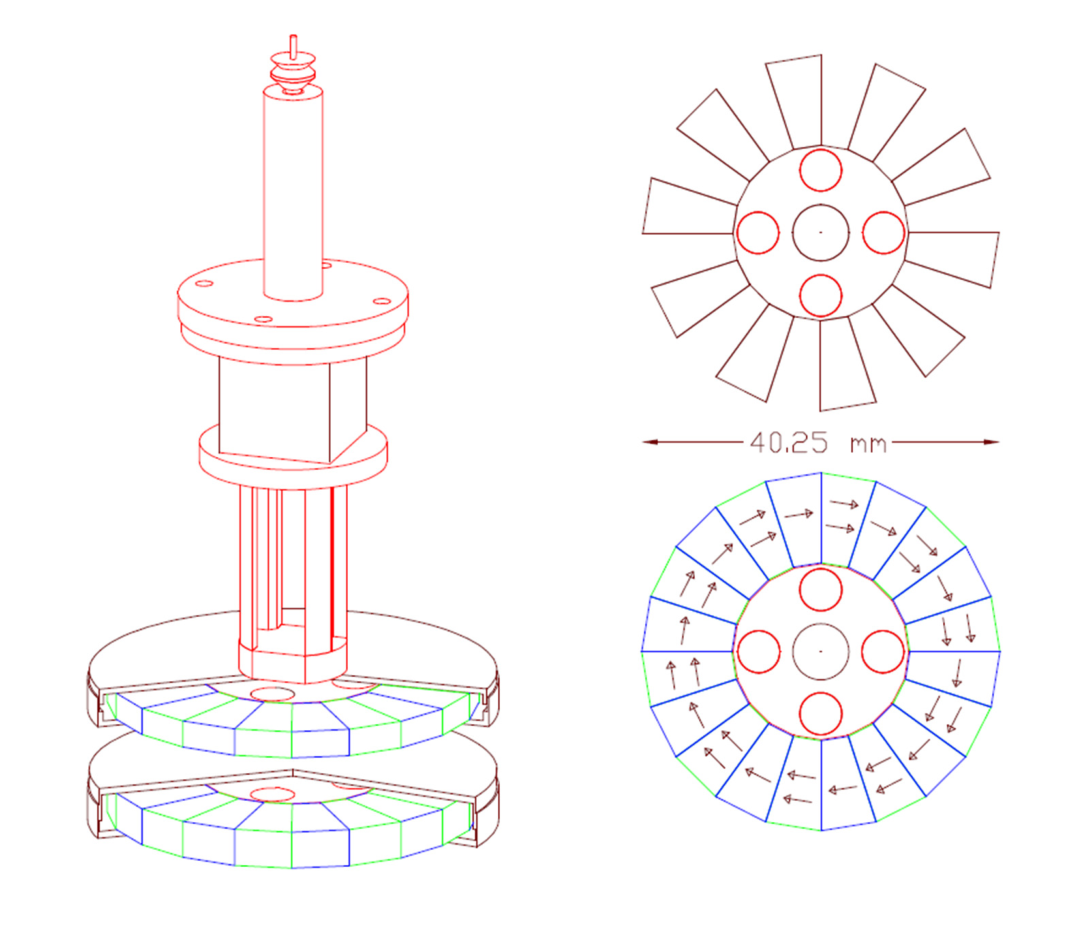
\includegraphics[width=0.42\textwidth]{Fig4.eps}
\end{center}
\caption{(color online). 
The spin-polarized torsion pendulum experimental setup from \citet{terrano_short-range_2015}. 
\textbf{Left}: The torsion pendulum (top) and the spin source (bottom). The torsion pendulum is suspended by a thin fiber, and a mirror cube is placed in the middle to detect the rotation angle. Laser light is reflected by the mirror and further detected by a position-sensitive sensor (not shown). Two sets of spin sources are covered by $\mu$-metal shielding (cut away to shown the internal sources). 
\textbf{Right}: The unpolarized source (top) and spin-polarized source (bottom). The unpolarized source is composed of gapped poles of copper to produce mass densities that alternate in the rotating frame, while the spin-polarized source consists of poles composed of Alnico (high density) and SmCo$_5$ (low density), which have different electron spin densities, with the arrows indicating the spin direction and density. 
The red circles represents the calibration cylinders.} 
\label{EW_setup}
\end{figure}



%%%%
\paragraph{Microscale mechanical oscillators}\label{METH1.SENS.MS.MMO}

To search for exotic forces on the microscale, one may use micro- and nano-fabricated sensors \cite{bachtold_mesoscopic_2022}. 
They can be used in cantilever mode \cite{chiaverini_new_2003} or in torsional mode \cite{long_upper_2003}, depending on the geometry of the sensor. 

The typical force sensitivity of microscale cantilever sensors is $\sim 100 \,\rm aN/\sqrt{Hz}$, \cite{chiaverini_new_2003}, while nanoscale resonators have achieved force sensitivities well below the $\rm aN/\sqrt{Hz}$ level in a cryogenic system \cite{moser_ultrasensitive_2013}. 

Microcantilever experiments to test gravity at short distances were conducted by \citet{chiaverini_new_2003}, where 0.355\,$\mu$m thick, 50\,$\mu$m wide and 250\,$\mu$m long single-crystal silicon oscillators were used as force sensors while a driven oscillating source mass consisting of alternating 100\,$\mu$m wide gold and silica bars was used to generate an alternating gravitational-type force.
In the torsional resonator experiment of \citet{long_upper_2003}, the lead source mass was modulated at high frequency by a piezoactuator. 
In addition, the cantilever itself does not depend on polarized spins; materials that have high net spin densities, such as ferromagnetic materials, can be used in the source \cite{ding_constraints_2020} or the sensor \cite{ren_search_2021} to search for spin-dependent interactions. 
%\LC{Check this sentence.} 
%\YS{I've checked and updated slightly.} 

%%%%
\paragraph{Levitated sensors}

Levitated particles are sensitive to forces and torques: sensors based on levitated spherical particles have achieved force sensitivities of $\rm 1.6\,aN/\sqrt{Hz}$ \cite{ranjit_zeptonewton_2016}, while levitated anisotropic particles can have torque sensitivities exceeding $\rm 10^{-27}\,N\cdot m/\sqrt{Hz}$ \cite{gonzalez-ballestero_levitodynamics_2021}. These sensors also showed potential for high acceleration sensitivity, for example $\sim \rm 10^{-10}\,g/\sqrt{Hz}$ \cite{timberlake_acceleration_2019}.
%\,[Timberlake et al, Appl. Phys. Lett. 115, 224101 (2019)]. 
Due to their exceptional sensitivity, levitated sensors have been suggested and used for investigating short-range forces (\citealp{geraci_short-range_2010}; \citealp{chen_ultrasensitive_2021},\citealp{yin_experiments_2022}).
%\cite{geraci_short-range_2010,chen_ultrasensitive_2021}. 

%\DB{We stopped here}

Because these types of optically levitated sensors do not have net spin, they are not normally used to search for spin-dependent forces; 
however, if a spin-polarized source is placed nearby, then it is possible to search for the monopole-dipole term $V_{9+10}$. 
An emerging type of levitated spin-based sensor is the levitated ferromagnetic sensor \cite{jackson_kimball_precessing_2016}, which is predicted to have an unprecedented sensitivity to spin-dependent forces due to the high spin density in the ferromagnetic material and its strongly correlated electron spins. 
%\DKIns{
The remarkable sensitivity of levitated ferromagnetic sensors is a result of the rapid averaging of quantum noise \cite{vinante_surpassing_2021}.
%}
This allows the levitated ferromagnetic torque sensor to ameliorate the detrimental effects of spin relaxation and spin-projection noise that are present in gas-phase atomic magnetometers.
Levitated ferromagnetic sensors have been proposed to search for spin-dependent fifth forces \cite{fadeev_ferromagnetic_2021} and dark matter \cite{ahrens_levitated_2024}, 
%\DKIns{
and potentially even test gravitational frame-dragging with intrinsic spins \cite{fadeev_gravity_2021}.
%}
%\cite{fadeev_ferromagnetic_2021,ahrens_levitated_2024}.%[Ahrens et al, arXiv:2401.03774]. 

%%%%%%%%%%%%%%%%%%%%%%%%%%%%%%%%%%%%%%%%%%%%%%%%%%%%%%
                      % S2. CM
%%%%%%%%%%%%%%%%%%%%%%%%%%%%%%%%%%%%%%%%%%%%%%%%%%%%%%

\subsubsection{Atomic magnetometers}
\label{METH1.SENS.AM}

%\YS{I'm not sure if we specifically discuss this point or not, but would it be worth discussing scalar vs vector magnetometers somewhere in this section (including from the point of view of, e.g., implications for the determination of directionality)?} \DB{If there is a bias field, asa is usually the case, a scalar magnetometer turns into a vector one. We might find a place to make this comment, but it is not clear whether this point is essential...}
%\YS{OK}

Atomic magnetometers use atomic vapors as the sensing medium. 
% can take the form of various vapour or gas-state sensors. 
% Here we focus on magnetometers that use atomic spins because the present review focuses on spin-related physics. 
%, and we ignore the atomic sensors that do not use spins, for instance the magnetometer using atomic transitions.
%Most of these sensors are in the gas state. 
The atoms can be paramagnetic, typically ground-state alkali atoms or metastable noble gases with unpaired electron spins. An alternative is ground-state diamagnetic atoms with nonzero nuclear spin. In some cases, a combined electron- and nuclear-spin medium is most beneficial. In this section,
% that use electron spins or diamagnetic atoms that utilise nuclear spins. 
we discuss the most commonly used alkali atom magnetometers and nuclear-spin sensors, such as mercury and noble-gas magnetometers. 
%\WJ{Add a general description of how this section is organised}

%%%%
\paragraph{Alkali-metal optically pumped magnetometers}\label{METH1.SENS.AM.AOPM}
% Alkali magnetometers use alkali atoms for sensing. 
In a typical setup, alkali atoms are enclosed in a glass or a fused silica cell and are pumped and probed with light. 
% The basic principle is that polarized light light interacts with the atomic ensemble and polarises the atomic spins.
A classic review of optical pumping was given by \citet{happer_optical_1972}, %\DKIns{
and a review of the nonlinear magneto-optical effects that are at the heart of modern atomic magnetometers was given by \citet{budker_resonant_2002}.
%}. 
%\,[W. Happer, Rev. Mod. Phys. 44, 169 (1972)]. 
Atomic spins precess under the influence of an external magnetic field and thus generate an oscillating magnetization that can be detected optically by Faraday rotation or by optical absorption \cite{dupont-roc_detection_1969}. 
%[Dupont-Roc, J., Haroche, S. & Cohen-Tannoudji, C., Detection of very weak magnetic fields (10-9 gauss) by Rb zero-field level crossing resonances, Phys. Lett. A 28, 638–639 (1969).]. 
Various types of alkali magnetometers work in different regimes to optimize specific parameters such as sensitivity, dynamic range, or bandwidth. 
For a review and explanation of the principles of atomic magnetometers, see (\citealp{budker_optical_2007}; \citealp{budker_optical_2013}).
%\citet{budker_optical_2007,budker_optical_2013}. 
%Ref.\,[Budker, Dmitry, and Michael Romalis. "Optical magnetometry." Nature physics 3.4 (2007): 227-234.
%],[1. Budker D, Jackson Kimball DF, eds. Optical Magnetometry. Cambridge University Press; 2013.],  

The fundamental sensitivity of an atomic magnetometer is limited by the spin-projection noise, which can be characterised as
 \cite{budker_sensing_2023}:
 %[Dmitry Budker and Mikhail G. Kozlov, arXiv:2011.11043v1]. 
\begin{equation}
    \delta B\approx \frac{\hbar}{g_F\mu_\textrm{B} \sqrt{2F}}\left(\frac{\Gamma}{N t}\right)^{1/2} \, ,
    \label{eq:sensitivity}
\end{equation}
where $g_F$ is Land\'{e} factor, $\mu_B$ is the Bohr magneton,  $F$ is the total angular momentum of the atom, $\Gamma$ is the spin-relaxation rate, $N$ is the number of the spins used in the measurement, and $t$ is the measurement time. 
To measure the magnetic field with better sensitivity, larger atomic numbers, longer coherence time, and longer integration time are desired. 
To increase the number of atoms, one can increase the saturated vapor pressure above an alkali-metal sample in the liquid or solid state by heating the vapor cell non-magnetically, for instance with hot flowing air, or using an AC electric heater operating at frequencies far removed from those of interest for the measurement. 
%\YS{What is non-magnetic heating? Is this just heating in the absence of an applied magnetic field?} 
%\WJ{Yes, but more importantly without inducing magnetic noises, typical way is by using twisted wire and tuning the heater driving frequency higher than the magnetometer bandwidth}
%\DKDel{to increase the atomic density, and at the same time use} 
Furthermore, a larger vapor cell can be used to increase the volume and thereby increase the total number of atoms $N$ participating in the measurement. 
Efforts are also directed towards decreasing the spin-relaxation rate (increasing the spin precession coherence time $T_2$). 
Typical ways to increase coherence time include coating the walls of the vapor cell with anti-relaxation materials, adding a buffer gas to slow down diffusion to the cell walls, and using larger cells \cite{walker_spin-exchange_1997}. 

A typical optically pumped atomic magnetometer,
%\DKDel{(here essentially a alkali-noble gas self-compensating comagnetometer)}, 
as shown in Fig.\,\ref{fig.comagnetometer}, uses a pump light beam and a probe light beam, and the vapor cell is enclosed within a multi-layer $\mu$-metal shielding to ensure the cell is in near-zero-field conditions and also to guarantee low residual magnetic noise. 
Coils are positioned inside the magnetic shielding to generate a well-controlled magnetic field. 
%\DKEdit{The}{
In the case illustrated in Fig.\,\ref{fig.comagnetometer},
%} 
pump laser light is circularly polarized, while the probe laser light is linearly polarized. 
%\DKIns{
There are many variations on optical pumping and probing schemes, including single-beam arrangements \cite{budker_nonlinear_1998}
%[add reference: Budker, Dmitry, Valeriy Yashchuk, and Max Zolotorev. ''Nonlinear magneto-optic effects with ultranarrow widths." Physical review letters 81.26 (1998): 5788.] 
and different choices of light polarizations optimized for different measurement goals \cite{ben-kish_dead-zone-free_2010},
%[add reference: Ben-Kish, A., and M. V. Romalis. "Dead-zone-free atomic magnetometry with simultaneous excitation of orientation and alignment resonances." Physical review letters 105.19 (2010): 193601.], 
as well as many different modulation schemes \cite{budker_nonlinear_2002,gawlik_nonlinear_2006}.
%[add references: Budker, D., et al. ``Nonlinear magneto-optical rotation with frequency-modulated light." Physical Review A 65.5 (2002): 055403; and Gawlik, Wojciech, et al. ``Nonlinear magneto-optical rotation with amplitude modulated light." Applied physics letters 88.13 (2006).].
%} 

\begin{figure} [!htbp]
\begin{center}
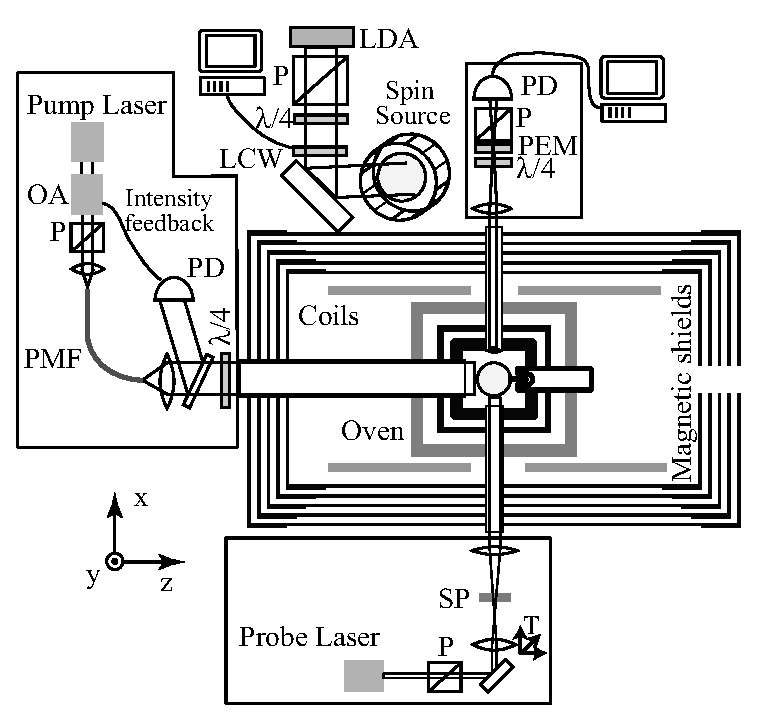
\includegraphics[width=0.48\textwidth]{Fig5.eps}
\end{center}
\caption{ The atomic comagnetometer experimental setup from \citet{vasilakis_limits_2009} used in a search for an exotic spin-dependent interaction. OA: optical amplifer, PMF: Polarization maintaining fiber, P: polarizaer, LDA: laser diode array, LCW: liquid crystal wave plate, PD: photodiode, SP: stress plate to control polarization of the probe beam, T: Translation stage to shift the probe beam, PEM: photoelastic modulator, $\lambda/4$: quarter-wave plate.}\label{fig.comagnetometer} 
\end{figure}

In this Review, we pay special attention to alkali magnetometers operating in the spin-exchange relaxation-free (SERF) regime, which are widely used in spin-dependent fifth-force searches. 
The SERF regime was discovered in 1973 (\citealp{happer_spin-exchange_1973}; \citealp{happer_effect_1977}) 
%\cite{happer_spin-exchange_1973,happer_effect_1977} 
%\,[Happer W., Tang H.. Spin-Exchange Shift and Narrowing of Magnetic Resonance Lines in Optically Pumped Alkali Vapors[J]. Physical Review Letters, 1973, V31(5): 273-276] [Happer W., Tam A. C.. Effect of Rapid Spin Exchange on the Magnetic-Resonance Spectrum of Alkali Vapors[J]. Physical Review A, 1977, V16(5): 1877-1891] 
and first demonstrated in a magnetometer by the Princeton group in 2002 \cite{allred_high-sensitivity_2002}. 
%[Allred J. C., Lyman R. N., Kornack T. W., et al. High-Sensitivity Atomic Magnetometer Unaffected by Spin-Exchange Relaxation[J]. Physical Review Letters, 2002, V89(13): 130801]. 
%\DKIns{
In the low-density case where the Larmor precession rate is faster than the spin-exchange rate [see, for example, \citet{budker_sensitive_2000}],
%[add reference: Budker, D., et al. ``Sensitive magnetometry based on nonlinear magneto-optical rotation.'' Physical Review A 62.4 (2000): 043403.]
when collisions transfer alkali atoms between ground-state hyperfine levels, the precessing atomic spins dephase since the ground state Land\'e factors $g_F$ have opposite signs.
%} 
In contrast, in the high-alkali-density SERF regime, the spin-exchange rate is faster than the Larmor precession rate: 
%\DKDel{, which effectively makes the atoms precess together and thus spin-exchange relaxation is diminished.} \DKIns{
the atoms are collisionally transferred back-and-forth between ground-state hyperfine levels many times during a single Larmor period. Thus the atoms collectively precess with a time-averaged spin and magnetic moment (nonzero due to the different statistical weights of the two ground-state Zeeman manifolds). In this way, the SERF regime avoids dephasing due to spin-exchange collisions, allowing operation at much higher atomic vapor densities (and hence larger $N$) without an overly large spin-relaxation rate $\Gamma$.
%} 

The requirements of the SERF regime are a relatively high alkali atom density
such that the spin-exchange rate is fast, and a sufficiently small magnetic field such that the Larmor frequency is small. 


Alkali atoms have valence electrons and nuclei with unpaired spins. 
%To deduce the fraction of spins contributing to the total atomic angular momentum, the 
The hyperfine interaction and the spin-temperature distribution should be considered to deduce the fraction of atomic spin due to the electron spin $\eta_e$ and nuclear spin $\eta_N$. 
In the nuclei, finding the fraction of neutron spin $\eta_n$ and proton spin $\eta_p$
%\DKDel{can be deduced by at least three approaches: a semiempirical approach \cite{stadnik_nuclear_2015}, a \textit{ab initio} nuclear shell model calculations \cite{jackson_kimball_nuclear_2015}, as well as a self-consistent mean field theory method \cite{brown_nuclear_2017}.} \DKIns{
requires input from nuclear theory \cite{jackson_kimball_nuclear_2015,brown_nuclear_2017}, although reasonable estimates are obtained for valence nucleons based on the single-particle approximation \cite{schmidt_uber_1937}.
%[add reference: Schmidt T 1937 Z. Phys. 106 358].
%}
%[brown et al,PRL 119, 192504 (2017)]}.

Data from experiments with thermal-vapor alkali spin sensors, such as alkali spin-exchange relaxation rates \cite{jackson_kimball_constraints_2010} and frequency-shift noise \cite{xiao_exotic_2024}, were used to search for exotic forces down to the atomic scale. \citet{kim_experimental_2019} and \citet{chu_experimental_2020} used BGO and DyIG sources, respectively, in conjunction with atomic magnetometers to search for spin-dependent force at a similar range. Atomic magnetometers in conjunction with SmCo$_5$ and iron-based electron spin sources were used to search for 10\,cm- and longer-range forces \cite{ji_constraints_2023}. Experiments using alkali comagnetometers are discussed in Sec.\,\ref{Sec:limits_main}.

%%%%
\paragraph{Nuclear spin magnetometers}

%\DKDel{Some modern atomic magnetometers utilize nuclear-spin-polarized diamagnetic atoms as the sensor, because their electron spins are paired and only the nuclear magnetic moment manifests, meaning that the atomic magnetic moment can be orders of magnitude smaller than that of paramagnetic atoms such as the alkalis.} 
%\DKIns{
Some atomic magnetometers used in precision searches for exotic spin-dependent interactions employ nuclear-spin-polarized diamagnetic atoms as sensors, owing to the paired nature of their electron spins, which results in cancellation of the electronic magnetic moment and exclusive manifestation of the nuclear magnetic moment. Consequently, the atomic magnetic moment is significantly reduced, often by several orders of magnitude, in comparison to magnetometers based on paramagnetic atoms such as alkalis.
%}
A small magnetic moment means better energy resolution for Zeeman-like interactions experiencing the same magnetic field noise; for further details, see the discussion around Eq.\,\eqref{eq:beff}. 
Vapor cells containing noble gas or mercury are often used because of the achievable high vapor density and long spin-coherence time. 
%\DKDel{Noble gases can remain in the gaseous state at pressures as high as 30\,atm.} 
%\DK{I believe that noble gases remain gaseous up to much higher pressures! This limit is probably more due to safety from preventing glass cells from exploding.}\LC{Dear Derek, thank you for your explanation.}
Commonly used noble-gas atoms include the spin-$1/2$ atoms $\rm ^{3}$He and $\rm ^{129}$Xe and the spin-$3/2$ atoms $\rm ^{21}$Ne and $\rm ^{131}$Xe, with multiple species sometimes used together to 
%\DKDel{suppress}{ 
measure, compensate, and subtract noise from
%} 
fluctuations in the magnetic field, i.e., operating in the comagnetometer mode, 
see Sec.\,\ref{METH1.SENS.AM.AC} for details.
%details of which can be found in Sec.\,\ref{METH1.SENS.AM.AC}.  %\DK{Comagnetometry doesn't necessarily ``suppress'' fluctuations in the magnetic field, only allows to substract or deal with them.}\LC{ok}

Noble-gas atoms can be polarized using spin-polarized alkali atoms via spin-exchange collisions \cite{walker_spin-exchange_1997}. 
%\,[Walker, Thad G., and William Happer. "Spin-exchange optical pumping of noble-gas nuclei." Reviews of modern physics 69.2 (1997): 629.]. 
The readout can be performed \textit{in situ} using alkali atoms \cite{vasilakis_limits_2009,wei_constraints_2022} or it can be done using external sensors such as superconducting quantum interference devices (SQUIDs) \cite{tullney_constraints_2013}. The \textit{in situ} readout method takes advantage of the Fermi contact interaction between the alkali electron and the noble gas nuclei. These sensors can work in the comagnetometer mode (see Sec.\,\ref{METH1.SENS.AM.AC}) or spin-amplifier mode (see Sec.\,\ref{METH1.SENS.AM.SMSA}). 
%\YS{Need to check hyperlink.} 
%\YS{This might be the first place in the main text where we use the acronym SQUID. We also use the term in Table~\ref{tabel_sensor} a bit earlier. Should we define it in one or both of these places?} 



%%%%
\paragraph{Atomic comagnetometers}\label{METH1.SENS.AM.AC}

Comagnetometers involving two (or more) %\DKEdit{systems}{ 
magnetically sensitive atomic species
%} 
operating together are widely used in fundamental physics, including in searches for fifth forces \cite{lee_improved_2018,wei_constraints_2022}, dark matter \cite{wu_search_2019,lee_laboratory_2023}
%\,[Lee, Junyi, et al. "Laboratory constraints on the neutron-spin coupling of fev-scale axions." Physical Review X 13.1 (2023): 011050.] 
and testing Lorentz invariance and $CPT$ violation \cite{brown_new_2010}. 
%\,[J. M. Brown, New Limit on Lorentz- and CPT-Violating Neutron Spin Interactions, PRL 105, 151604 (2010)] 

Comagnetometers can be configured to be insensitive to normal magnetic fields, while retaining sensitivity to exotic physics interactions that do not directly couple to the magnetic moment of the atoms. 
A comagnetometer can utilise two atomic species, for instance, two species of noble gases, such as $^{3}$ He and $^{129}$ Xe, or two isotopes of the same species, such as $^{129}$Xe and $^{131}$Xe. 
A comagnetometer can also use two atomic levels in a single atom, such as the two hyperfine levels of $^{87}$Rb \cite{wang_single-species_2020}
%[Wang et al, PRL 124, 193002 (2020)] 
and $^{133}$Cs \cite{bevington_dual-frequency_2020},
%\YS{I think this is correct - is there a suitable reference(s) for this? Another example is an atomic comagnetometer based on the $F=3$ and $F=4$ hyperfine states of $^{133}$Cs demonstrated in \citet{bevington_dual-frequency_2020}.}
%\url{https://journals.aps.org/pra/abstract/10.1103/PhysRevA.102.032804}.
or even molecular states with different total nuclear angular momentum in an isotopologue of acetonitrile \cite{wu_nuclear-spin_2018}, which was used for ultralight dark matter search \cite{wu_search_2019}.
%\YS{I'm not sure what exactly we mean in this phrase, but a comagnetometer based on states with different total nuclear angular momentum in an isotopologue of acetonitrile has been demonstrated and utilised in an ultralight dark matter search . 
The spin-polarized torsion pendulum system described in Secs.\,\ref{METH1.SOUR.ESS} and \ref{Sec:torsion_pendula_sensors} can also generally be thought of as comagnetometers because the spin and orbital magnetic moments cancel each other, which renders the spin pendulum insensitive to normal magnetic fields whilst being sensitive to exotic pseudo-magnetic fields.
%and keeps its insensitivity to magnetic field but sensitive to exotic field. 

In this section, we focus on atomic comagnetometers. 
For earlier reviews of comagnetometers in the context of fundamental physics, see \citet{terrano_comagnetometer_2022}; \citet{huang_axion-like_2024}.
%\cite{terrano_comagnetometer_2022,huang_axionlike_2023}. %[Huang, Xiaofei, et al. "Axionlike Particle Detection in Alkali-Noble-Gas Haloscopes." arXiv preprint arXiv:2312.09491 (2023).]. 
With regard to the basic operating principle, comagnetometers can be characterized according to the way the comparison is done. \citet{terrano_comagnetometer_2022} distinguish the ``clock-comparison'' and  the ``quantization-axis'' self-compensation (SC) method, where the magnetization axis of the compensating species automatically rotates to cancel an external field.
%There are two types of comparison style, namely the energy splitting style or quantization axis style, the former one is also called the clock comparison method and the latter one is also called self-compensation method \cite{terrano_comagnetometer_2022}. 

The clock-comparison method typically compares the precession frequencies of two atomic species; since the gyromagnetic ratios of these species are not the same, their precession frequencies are also different. 
By comparing the two precession frequencies, one can cancel out the sensitivity to the magnetic field, whilst retaining sensitivity to an exotic field. %\LC{Are $\nu_1$, B, $b_1$ below vectors? } \YS{From what I can tell, these quantities aren't vectors.} 
The general dynamics of the two species (which could even be different states in the same atom) can be described according to the relations $\omega_1= \gamma_1(B +  b_1)$ and $\omega_2=\gamma_2 (B+ b_2) $, 
%\DKIns{
neglecting any other sources of non-magnetic spin precession (which inevitably lead to a wide range of systematic errors), and where we assume the directions of the magnetic field vector and pseudo-magnetic field vector are aligned along the comagnetometer sensitive axis.
%}
Here $\omega_1$, $\omega_2$ and $\gamma_1$, $\gamma_2$ are the precession frequencies and gyromagnetic ratios of the two species, respectively. 
The two species sense the same magnetic field $B$, but typically see different effective pseudo-magnetic fields due to the exotic spin-dependent interaction. 
The exotic potential $V$ will be sensed by the two species as effective magnetic fields $b_1 = V \, \eta_1 /\gamma_1 \hbar$, and $b_2 = V \, \eta_2 /\gamma_2 \hbar$, respectively (where $\eta_1$ and $\eta_2$ are the fractions of spin polarization for these two species).
%we will only have $\nu_1/\nu_2=\gamma_1/\gamma_2$ when the fraction of angular momentum of spins applies $\eta_1=\eta_2$, which is not generally the case for comagnetometers. 
%\YS{We should define the quantity $V$ here. It would also be nice to remind the reader of the definition of $\eta_{1,2}$ here - is this the fraction of magnetism due to the spin magnetism from a certain fermion species? The equations for $\nu_{1,2}$ earlier on in this paragraph are technically incomplete, since the effective field is, generally speaking, not the same for electron and nucleon spins. There should be some sort of summation over fermion species/types in these formulae, which is important for magnetometers with both unpaired electron spins and nonzero nuclear spin.} 
%\WJ{The clock comparison experiment normally do not use the comparison of electron and proton, so probabily is is okay}
%\LC{The equation below need check.} 
%\YS{Just checking quickly, I find $\nu_1 / \nu_2 \approx \gamma_1 / \gamma_2 \left[1 - V/(\hbar \nu_2) \times \left(\eta_2 - \eta_1 \gamma_2 / \gamma_1 \right) \right]$. (The approximate sign is to indicate that this is to leading order in $\eta_{1,2}$; i.e., discarding second- and higher-order terms in $\eta_{1,2}$).} 
%If we \YS{define?} $g_{12}\gamma_1/\gamma_2$, the frequency ratio can be expressed as $\nu_1/\nu_2=-g_{12}-V\cdot (\eta_1-g_{12}\eta_2)/\nu_2$, 
%\DKDel{the ratio between the gyromagnetic ratios of two species is $\rho=\gamma_1/\gamma_2$, and} 
The frequency ratio can be expressed as 
%\LC{Derek newly added the following two equations:}
%\begin{equation}  \omega_1 / \omega_2 \approx -\rho-\frac{1-\rho}{\omega_2}\Omega_{\parallel}-\frac{\eta_1-\rho\eta_2}{\omega_2}V_{\rm{eff}}/\hbar\,.\end{equation}
\begin{align}\label{Eq:fre-ratio}
    \frac{\omega_1}{\omega_2} &= \frac{\gamma_1}{\gamma_2} \frac{B + b_1}{B + b_2} \approx \frac{\gamma_1}{\gamma_2} \left( 1 + \frac{b_1}{B} - \frac{b_2}{B}  \right) \notag\\
    &\approx \frac{\gamma_1}{\gamma_2} \left[ 1 + V\left( \frac{\eta_1}{\hbar\omega_1} - \frac{\eta_2}{\hbar\omega_2} \right) \right]~.
\end{align}
%\DK{I think the revised equation is far more transparent, and maybe more correct, than what was written earlier :).}
%\WJ{Beautiful, thanks!}
Here, the approximate sign indicates that this is to leading order in $\eta_{1,2}V$; i.e., discarding second- and higher-order terms. 
%\DKDel{, $\Omega_{\parallel}$ is the projection of the rotation of the frame along the sensitive axis of the comagnetometer.} 
From Eq.\,\eqref{Eq:fre-ratio}, we can extract the exotic spin-dependent potential $V$ by comparing two precession frequencies. 
%\YS{As a side question, is the factor of $1/\hbar$ in the definitions of $b_{1,2}$ above necessary?} 

%%%%


%Take a $^{129}$Xe-$^{131}$Xe comagnetometer as an example \cite{zhang_search_2023}, the two isotopes of Xe atoms are inclosed in the same cell of Rb and are spin polarized and magnetically read out by Rb atoms.   

The comagnetometer of \citet{venema_search_1992} employing both $\rm ^{199}Hg$ and $\rm ^{201}Hg$ atoms is of the clock-comparison type. 
The atoms are polarized with ultraviolet light [the physics of how nuclei are polarized in such a process is discussed by \citet{budker_atomic_2010} in Prob.\,3.20]. 
A typical atomic density of Hg is on the order of $10^{13} - 10^{14}\,\rm{cm}^{-3}$, similar to that of alkali atoms but lower than that of noble gas atoms.
In contrast to the indirect probing of the noble-gas spins in alkali-noble gas sensors, Hg atoms are directly probed with linearly polarized light via %\DKEdit{the polarization-rotation effect}{
optical rotation.
%}.
%\LC{Is \citet{zhang_search_2023} the same type of comagnetometer? or improved version?} 
\citet{venema_search_1992} used the Earth as the mass source of the long-range exotic force. In such experiments, since the source cannot be modulated, a typical approach involves modulating the sensitive axis of the sensor. This is done in a configuration where the Earth rotation axis is parallel to the sensitive axis of the comagnetometer, minimizing the uncertainties due to tilt errors caused by gyroscopic effects associated with the Earth rotation. The magnetic field direction is periodically inverted to modulate 
%the \DKEdit{effects of the exotic fields arising from the Earth}{ 
the relative sign of the magnetic and non-magnetic torques causing precession.
%}. 
Other experiments that used Earth as the source employed a $^{85}$Rb-$^{87}$Rb dual-isotope alkali comagnetometer \cite{jackson_kimball_constraints_2017} or a $^{129}$Xe-$^{131}$Xe dual-isotope noble-gas comagnetometer \cite{zhang_search_2023} to search for long-range forces. \citet{wu_nuclear-spin_2018} proposed using the $^{1}$H-$^{13}$C nuclei in liquid-state acetonitrile that can work as a comagnetometer for long-range forces, and \citet{wang_single-species_2020} proposed using dual hyperfine levels of $^{87}$Rb. 

Some experiments searching for local Lorentz invariance, or testing the $CPT$ symmetry, also employ modulation of the comagnetometer sensitive direction. Such experiments include $^{129}$Xe-$^3$He comagnetometery \cite{allmendinger_new_2014}, $^{199}$Hg-$^{133}$Cs comagnetometery \cite{peck_limits_2012}, and  K-$^3$He and K-Rb-$^{21}$Ne comagnetometers with self-compensation  \cite{brown_new_2010,smiciklas_new_2011}.  In some cases, the data from such experiments can be re-analyzed and re-interpreted as a search for long-range exotic interactions sources by the Earth, the Sun, or the Moon. For instance, \citet{hunter_using_2013,hunter_using_2014} reanalyzed the data from \citet{peck_limits_2012} and \citet{heckel_preferred-frame_2008} assuming geoelectrons as the source of exotic fields, and \citet{wu_new_2023} reanalyzed the data from \cite{allmendinger_new_2014} taking the solar and lunar masses as sources.
% \WJ{Similar to that of search for spin-gravity experiments, many experiment testing new physics field, such as that of testing local Lorentz invaricance, or CPT violation experiments also modulate the sensor direction, for instance that of $^{129}$Xe-$^3$He comagnetometer by \citet{allmendinger_new_2014}, and that of a $^{199}$Hg-$^{133}$Cs comagnetometer by \citet{peck_limits_2012}, and that of a self-compensation K-$^3$He comagnetometer by \cite{brown_new_2010}. In principle, these data can be reanalysed if taking the earth or even the moon and sun as the mass source for the long range forces. For instance, \citet{hunter_using_2013,hunter_using_2014} by taking the geoelectron as the source when reanalyzing the data from \cite{peck_limits_2012} and \cite{heckel_preferred-frame_2008}, and \citet{wu_new_2023} reanalyzed the data from \cite{allmendinger_new_2014}when taking the solar and lunar mass as the source.}

Other experiments probing shorter-scale distances include those of \citet{bulatowicz_laboratory_2013} who used $^{129}$Xe-$^{131}$Xe comagnetometers with a SQUID probe and zirconia rod source to search for mm-scale forces, \citet{tullney_constraints_2013} who used a $^{3}$He-$^{129}$Xe co-magenetomter and BGO sources, and  \citet{feng_search_2022} who used $^{129}$Xe-$^{131}$Xe-Rb comagnetometer and BGO sources to search in a similar force range. 


%\YS{I didn't find any reference in \citet{zhang_search_2023} about using a Romalis' type self-compensating comagnetometer. It looks like \citet{zhang_search_2023} use a $^{129}$Xe-$^{131}$Xe-Rb comagnetometer. This looks more advanced than the $^{199}$Hg-$^{201}$Hg comagnetometer used in \cite{venema_search_1992}. It may be useful to compare the $^{129}$Xe-$^{131}$Xe-Rb comagnetometer used in \citet{zhang_search_2023} with the similar ones of \cite{feng_search_2022} and  described in the paragraph below.} 
%\LC{Content cut from the result section cut to here for reference: \citet{zhang_search_2023} measured the nuclear-spin precession frequencies of two Xe isotopes in an applied magnetic field that was aligned parallel to Earth's rotation axis in order to reduce systematic errors caused by gyroscopic effects. The team then took the ratio of the two precession frequencies and reversed the direction of the magnetic field, measuring the difference between the ratios corresponding to the two different field directions. This difference is proportional to the magnitude of precession caused by nonmagnetic effects, such as that arising from a monopole-dipole coupling of the Xe spins to the Earth.}

%\LC{\citet{feng_search_2022} focused on the ratio $R$ between the precession frequencies of the two Xe isotopes, $^{129}$Xe and $^{131}$Xe, correlated with the position of the BGO mass. $R$ is expressed as $(\gamma_{129}B +X_{129})/(\gamma_{131}B +X_{131})$ where the $X_i$ denote the frequency shifts of the corresponding $^i$Xe isotopes due to exotic interactions, and the $\gamma_{i}$ represent the nuclear gyromagnetic ratios. In the measurement sequence, together with the position of the BGO mass, the bias field direction and the pumping beam polarization are periodically switched. 
%The comagnetometer system used by \citet{feng_search_2022} was previously utilized to search for a monopole-dipole interaction by \citet{bulatowicz_laboratory_2013}. However, \citet{feng_search_2022} employed a modulated Rb polarization scheme \cite{limes_3mathrmhetextensuremath-129mathrmxe_2018} and designed the measurement sequence to reduce the systematic effect.} 
%\YS{Which specific systematic effect(s)?} 

A self-compensating SERF comagnetometer was first demonstrated by \citet{kornack_dynamics_2002}. 
The configuration of a typical alkali-noble-gas comagnetometer setup is shown in Fig.\,\ref{fig.comagnetometer}.
It operates on the principle that for sufficiently slow changes in the magnetic field, the noble-gas spins follow the changing magnetic field direction. 
%\DKDel{due to small magnetic field components transverse to the polarization direction}. \DKDel{The noble-gas %\YS{what do we mean by ``negative'' magnetic moment in this case?} 
%magnetic moments rotates such that from the point of view of the probe atoms, the magnetic disturbance is compensated.} \DKIns{
If the noble-gas magnetization and applied magnetic field are tuned so that they approximately cancel one another, the alkali atoms experience a net zero field environment, which is automatically undisturbed if the magnetic field adiabatically changes direction since the noble-gas magnetization follows the field and compensates it.
%}
To leading order, the response of the probe alkali atoms (specifically, the polarization along the $x$-axis) is given by \cite{vasilakis_limits_2009}: 
\begin{equation}
    P_x^e=\frac{P_z^e\gamma_e}{R_{tot}}\left(b_y^N-b_y^e+\frac{\Omega_y}{\gamma_N}\right)\,,
    \label{eq.SC}
\end{equation}
where $P_x^e$ and $P_z^e$ are the polarizations of alkali along x- and z- axis, while $b_y^N$ and $b_y^e$ are the pseudomagnetic field from the exotic field,
%\LC{Is this ``exotic physics field" a widely understood concept? Do we have a general phrase with the same meaning used in this review?}\WJ{I rephrased as pseudomagnetic field from the exotic field.}
along the y-axis that are sensed by the alkali and noble gas nuclei, respectively, $R_{tot}$ is the total relaxation rate, $\Omega_y$ is the frequency of the apparatus rotation along the $y$ axis (the magnetometer is also essentially an atomic gyroscope), $\gamma_e$ and $\gamma_N$ are the gyromagnetic ratio of alkali and noble gas atoms respectively.
Previous comagnetometers mainly suppressed low-frequency magnetic noise.
A novel atomic comagnetometer \cite{qin_new_2024}, based on coupling between alkali-metal and noble-gas spins, extends this suppression to higher frequencies, up to 100\,Hz.

Among the fifth-force experiments that employed self-compensating comagnetometers are that of \citet{vasilakis_limits_2009} who used polarized $^{3}$He as the source and placed constraints on dipole-dipole interactions between nucleon spins; the experiment of \citet{lee_improved_2018} who used lead sources to place constraints on monopole-dipole interactions between nucleon spin and nucleon mass; the experiment of \citet{almasi_new_2020} who used an iron shielded SmCo-magnet source and placed constraints on dipole-dipole interactions between neutrons and electrons; and the work of \citet{wei_constraints_2022} who utilized a tungsten-ring source and placed constraints on velocity-dependent interactions between unpolarized nucleons and neutron/proton spins. 

%\LCa{and superconducting quantum interference devices [29–31].--from \cite{chu_proposal_2022}}
%\YS{Do we discuss SQUID sensors in detail anywhere in this review? They are mentioned in passing many times and appear, e.g., in Table~\ref{tabel_sensor}. Maybe it might be helpful to have a brief standalone subsection on SQUIDs?} 

%\LCa{how about trapped ion system, such as \cite{kotler_measurement_2014}?}
%\YS{I think we discuss this paper in Sec.~\ref{METH2.PM.TI}.} 

%%%%
\paragraph{Noble-gas spin masers and amplifiers}\label{METH1.SENS.AM.SMSA}

%\paragraph{\WJ{Other sensors using nuclear magnetic resonance}}\label{METH1.SENS.AM.SMSA}

In addition to the comagnetometer regime previously discussed, polarized nuclei can operate in various other regimes tailored for specific objectives. For example, resonance feedback from coils and resonance circuits is utilized in the maser regime, as detailed by \citet{glenday_limits_2008}. In the nuclear magnetic resonance (NMR)-amplifier mode, the effective magnetic field of an exotic interaction can be resonantly amplified at the NMR frequency. This category of sensors includes those employing external pickup-coil readout methods \cite{budker_proposal_2014,arvanitaki_resonantly_2014}, as well as those utilizing an alkali \textit{in-situ} readout method, also referred to as a ``spin-based amplifier'' by \citet{jiang_search_2021,su_search_2021}.
The idea of the spin-based amplifier is that a feeble field acting upon a highly polarized dense spin sample with a long relaxation time rotates the magnetization of the sample. This rotation is detected with a magnetometer that senses the field of the polarized sample that is much larger than the field that caused the rotation. This way, the real or effective magnetic field is amplified. 

%\DKDel{It is important to note that the clock-comparison comagnetometers which utilizes dual nuclear spins also employ magnetic resonance of two species. However, it operates in a regime that allows for precise cancelation of the effect of normal magnetic field by frequency comparison, in contrast to the NMR amplifier, which enhances the signal amplitude.} \DK{I don't think that this is actually a meaningful distinction: the spin masers and spin amplifiers are essentially clock comparison experiments with added amplification techniques. I would just cut out this paragraph.} 

Generally, electron spins can also serve as transducers of exotic fields. For instance, ferromagnetic materials can be used to augment the coupling of electron spins with exotic fields, as demonstrated by \citet{chui_experimental_1993} and \citet{gramolin_search_2021}. These applications are further discussed in the section on solid-state electron spin sensors (Sec.\,\ref{METH1.SENS.SS}).

A nuclear spin-based sensor, with spins initially oriented along a leading magnetic field, develops transverse magnetization when subjected to a resonant oscillating magnetic field, as described, for example, by \citet{arvanitaki_resonantly_2014}.
%\DKDel{\begin{equation}
%    M_x(t) \approx \frac{1}{2}n p\mu_N \gamma_N b_N T_2(e^{-t/T_1}-e^{-t/T_2}) \cos(\omega t) \, , 
%    \label{eq.spin.amp}
%\end{equation}
%where $n$ is the spin density in the sample, $p$ is the polarization of the sample, and $\mu_N$ is the magnetic dipole moment of the relevant nuclei,
%\LC{is this $\mu_N$ as the previous $\mu$, if so better use the same one? } 
%$b_N$ is the effective magnetic field applied on the nuclei, $T_1$ and $T_2$ are the longitudinal and transverse coherence times, respectively.} 
%\LC{Derek delete the equation here. I comment the above equation out because \DKDel{xx} causes compile problem when it contains an equation.}
%\DK{I would delete the equation and description: it doesn't add to the narrative and it introduces new notation for essentially the same physics as described by earlier equations, needlessly complicating things! If the reader needs more details they can read the reference. Not needed here I think.} 
The magnetization of the nuclei can be read out with external or \textit{in-situ} magnetometers.

\textit{In-situ} readout of the alkali-noble gas magnetometers offers the advantage of an additional enhancement factor due to the Fermi-contact interaction between noble gases and alkali atoms. Amplification factors for magnetic fields and pseudo-magnetic fields in a $^{129}$Xe-Rb system have been reported in the range of 100-5400 \cite{su_review_2022}. 
%[su et al, https://doi.org/10.1007/s11432-022-3550-1]. 
This amplification scheme is generic and can be applied to a wide range of noble gas isotopes, which could further improve signal amplification by factors of $10^4$ with $^{21}$Ne and $10^6$ with $^3$He \cite{jiang_search_2021}. While both spin-based amplifiers and self-compensating comagnetometers (\citealp{vasilakis_limits_2009}; \citealp{lee_improved_2018}; \citealp{almasi_new_2020}; \citealp{xu_constraining_2023})
%\cite{vasilakis_limits_2009,lee_improved_2018,almasi_new_2020,xu_constraining_2023}
utilize overlapping spin ensembles (e.g., $^{129}$Xe-$^{87}$Rb), the former have a wider range of operational bias fields. In the K-Rb-$^{21}$Ne system, \citet{wei_dark_2023} identified a hybrid spin resonance distinct from the self-compensating regime. Under the conditions of hybrid spin resonance, the nuclear and electron precession frequencies coincide, leading to an increased linewidth of the noble gas, enabling dark matter search over a comparably much wider mass range \cite{wei_dark_2023}. Alkali-noble gas spin amplifiers using different types of species are useful in searches for axion-like dark matter (\citealp{jiang_search_2021}, \citeyear{jiang_floquet_2022}; \citealp{wei_dark_2023}; \citealp{huang_axion-like_2024}),
%\cite{jiang_search_2021,jiang_floquet_2022,wei_dark_2023,huang_axion-like_2023},
as well as exotic spin-dependent forces \cite{su_search_2021,wang_search_2023-1,wang_search_2023}.

Such type of spin amplifiers use a scheme in which nuclear spins and the detector spatially overlap in the same vapor cell, providing two significant advantages: nuclear spins can be directly hyperpolarized to achieve a polarization of 0.1–0.3 by spin-exchange optical pumping; nuclear spin signals can be enhanced due to a large Fermi contact enhancement factor, detected \textit{in-situ} with an atomic magnetometer.

%A selection of experiments utilizing alkali-noble gas atoms are listed in Tab.\,\ref{tabel_sensor}. The amplification factor for an exotic field in the self-compensating mode is near unity, which can be understood in a picture that both the resonance frequency and linewidth are about 1\,Hz and there is no amplification at sub 1\,Hz frequencies. In the NMR mode, larger leading fields are typically used, so that the resonance frequency is greater than the linewidth, so there is a resonance amplification. \DB{All the prose here needs to be carefully checked for accuracy and clarity...} \DK{To be honest, I found this paragraph to be quite unclear: it seems to suggest that it is obvious to the reader the relationship between resonance frequency, linewidth, and amplification. That relationship is at least not obvious to me. Could you revise and explain more clearly? The Fermi-contact interaction plays a role in all spin-exchange-optically pumped and probed experiments, so this idea of amplification has more to it than that. We have to be very clear about this. Is there really some advantage over SERF comagnetometers beyond the enhanced bandwidth? Or is the amplification merely with respect to the readout of the magnetization as compared to a direct measurement of the magnetic field by an external magnetometer?}
%\WJ{Dear all, I removed this discussion since it is not related to the major story here. The table is revised without mentioning the amplification factor, thus the discussion of this parameter is not included in this review.}

Other %spin-amplification
magnetic resonance experiments for exotic physics searches include the CASPEr experiment that uses hyperpolarized liquid-state Xe \cite{garcon_cosmic_2017}
and the ARIADNE experiment that uses polarized $^3$He \cite{arvanitaki_resonantly_2014} 
%as the amplification medium 
for short-range spin-dependent forces from both spin-polarized and spin-unpolarized sources. 
%\DK{Again, I am not sure about how we are thinking about the ``amplification'' concept. These are both experiments using spin-polarized samples and NMR. What is the essence of the amplification we're talking about? Also maybe consider mentioning the SHAFT experiment in this context \cite{gramolin_search_2021}?}
%\WJ{Dear Derek and Dima, I agree with Derek and removed the amplification factor discussions in the paragraph and in the table, and changed to a general magnetic resonance. \cite{gramolin_search_2021} is mentioned in the ferromagnetic material paragraph below.}


%%%%%%%%%%%%%%%%%%%%%%%%%%%%%%%%%%%%%%%%%%%%%%%%%%%%%%
                      % S3. 
%%%%%%%%%%%%%%%%%%%%%%%%%%%%%%%%%%%%%%%%%%%%%%%%%%%%%%


\subsubsection{Solid-state electron spin sensors}
\label{METH1.SENS.SS}

\paragraph{Ferromagnetic material}
Generally, the 
%\DKEdit{magnetic moment}{ 
magnetism
%} 
of a ferromagnet is dominated by unpaired electron spins, and thus ferromagnets can be 
%\DKIns{
used as sources and sensors based on polarized
%}  \DKEdit{electron-spin-based materials}{ 
electron spins
%} \DKDel{In fact, there are many ways, magnets can be used} 
for dark-matter (\citealp{gramolin_search_2021}; \citealp{bloch_scalar_2023})
%\cite{gramolin_search_2021,bloch_scalar_2023} 
and exotic spin-dependent force searches \cite{fadeev_ferromagnetic_2021}.

% A well known electron spin based amplifier is the electromagnet, which can significantly enhance the applied magnetic field. 
% In the case of a general magnetic material, we can take the amplification factor to be given by the magnetic susceptibility that applies
% %\YS{I think relative permeability is normally denoted by the symbol $\mu_r$, whereas $\mu$ is the permeability. I'm also not sure of the origins of Eq.~(\ref{relative_permeability}). In a linear medium, I think the relevant equations read $\mu \approx \v{B}/\v{H}$ and $\mu_r \approx \v{B}_\textrm{in} / \v{B}_\textrm{out}$. Please check.} 
% \begin{equation}
% \label{relative_permeability}
%     \chi \simeq \frac{M}{H}\,.
% \end{equation}

The core of an electromagnet consists of a magnetically soft material with oriented magnetic domains producing magnetization that reinforces the applied field, thereby enhancing the applied magnetic field. 
A magnet made of a hard magnetic material, if it can freely move in space with small mechanical energy dissipation, can also be treated as an amplifier and can be used as a high-sensitivity magnetometer 
(\citealp{jackson_kimball_precessing_2016}; \citealp{fadeev_ferromagnetic_2021}; \citealp{vinante_surpassing_2021}; \citealp{ahrens_levitated_2024}).
%\cite{jackson_kimball_precessing_2016,fadeev_ferromagnetic_2021}. 
In their pioneering experiments, \citet{vorobyov_new_1988} used ferromagnetic permalloy material as a transducer and a SQUID to read out its magnetization change. 
\citet{chui_experimental_1993} utilized paramagnetic terbium fluoride (TbF$_3$) as a transducer material and Dy$_6$Fe$_{23}$ as a spin-polarized source to search for electron-spin-dependent forces. 
\citet{quax_collaboration_axion_2020} (QUaerere AXion, or: QUest for AXions) used ferromagnetic yttrium iron garnet (YIG) as an amplifier in their axion dark matter search, but in their case by searching for the axion coupling to the electron spins in YIG. They also used Gd$_2$SiO$_5$, which has a magnetic susceptibility of $\chi \approx 0.7$ as a transducer for exotic interaction research; see Sec.,\ref{gpgs_e-N}. 
The experiment of \citet{gramolin_search_2021} used a ferromagnetic material to enhance the currents generated by ALP dark matter via the ALP-photon coupling.
In addition, paramagnetic materials, for instance Gd$_{3}$Ga$_{5}$O$_{12}$, which has a susceptibility of $\chi \approx 0.53$ at 3.1\,K, are also proposed as transducers of exotic spin dependent forces even without amplification \cite{chu_search_2015}. In these experiments, the signals/magnetization from the transducer materials are measured with SQUID magnetometers.

%%%%
\paragraph{Sensing with nitrogen-vacancy (NV) centers in diamond}\label{METH1.SENS.SS.NV}

The NV center in the diamond-crystalline lattice is a point defect with unique optical and magnetic properties, enabling the detection of small magnetic fields with high sensitivity and on short distance scales \cite{degen_quantum_2017,barry_sensitivity_2020}. 
NV-diamond-based sensors have emerged in recent years as a promising platform to probe exotic interactions at the micrometer scale 
(\citealp{rong_searching_2018}; \citealp{rong_constraints_2018}; \citealp{chen_optomechanical_2020}; \citealp{rong_observation_2020}; \citealp{jiao_experimental_2021}; \citealp{chen_ultrasensitive_2021}; \citealp{liang_new_2022}; \citealp{chu_proposal_2022}; \citealp{guo_searching_2024}; \citealp{huang_new_2024}).
%\cite{rong_searching_2018,rong_constraints_2018,chen_optomechanical_2020,rong_observation_2020,jiao_experimental_2021,chen_ultrasensitive_2021,liang_new_2022,chu_proposal_2022,guo_searching_2024,huang_new_2024}. 
NV-center magnetometry, and especially single-NV-center magnetometry, offers high spatial resolution, down to atomic scale, exceeding that of atomic vapor-cell magnetometry. 
Single-NV-center magnetometers have magnetic-field sensitivity down to $\sim 0.5\,\rm nT/\sqrt{Hz}$ \cite{zhao_sub-nanotesla_2023}. Although not as sensitive as atomic magnetometers (whose sensitivities reach sub-fT$\rm/\sqrt{Hz}$ for macroscopic fields), diamond sensors are useful for probing exotic forces at much shorter length scales.
%it can reach some short range parameter that atomic magnetometer cannot reach. 

%The principle is like that of atomic magnetometer that utilised the pumping and probe techniques. The sensor consists of a substitutional nitrogen atom with an adjacent vacancy site in the diamond crystal lattice. The NV centers are observed to possess three charge states $NV^+$, $NV^0$, and $NV^-$\cite{barry_sensitivity_2020}. The $NV^-$ state is mostly utilized for its stable coherent optical transition, long-lived spin coherence, and mechanisms for coupling to external degrees of freedom\cite{barry_sensitivity_2020}, thus we refer to $NV^-$ when we talk about NV centers later. 

%The ground state of the NV center is an electron-spin triplet state $^3A_2$ with three substates $m_s=0$ and $m_s=\pm 1$. A static magnetic field $B_0$ is applied along the NV symmetry axis to remove the degeneracy of the $m_s=\pm 1$ spin states. The spin states $m_s=0$ and $m_s=-1$ (or $m_s=+1$, here we use the former as an example) are encoded as a quantum sensor. Microwave pulses with frequency matching the transition between $m_s=0$ and $m_s=-1$ are delivered to manipulate the state of the quantum sensor. The $m_s=+1$ state remains idle due to the large detuning. A laser pulse can be applied to pump the NV center from $^3A_2$ to the excited state $^3E$. When the NV center decays back to $^3A_2$, photoluminescence can be detected. 
%Here, through the spin-state-dependent intersystem crossing, states $m_s=\pm 1$ is possible to decay into $m_s=0$ through metastable states $ ^1 A$ and $^1E$ \cite{barry_sensitivity_2020} while state $m_s=0$ only decay back to $m_s=0$. So optical process can be utilized to realize state initialization with spin-polarized into $m_s=0$. Also, the decay through metastable states is a non-radiative transition, so the fluorescence from $m_s=\pm 1$ would be weaker than $m_s=0$. Therefore the optical process can be utilized to realize readout of this quantum sensor.

\begin{figure} [!htbp]
\begin{center}
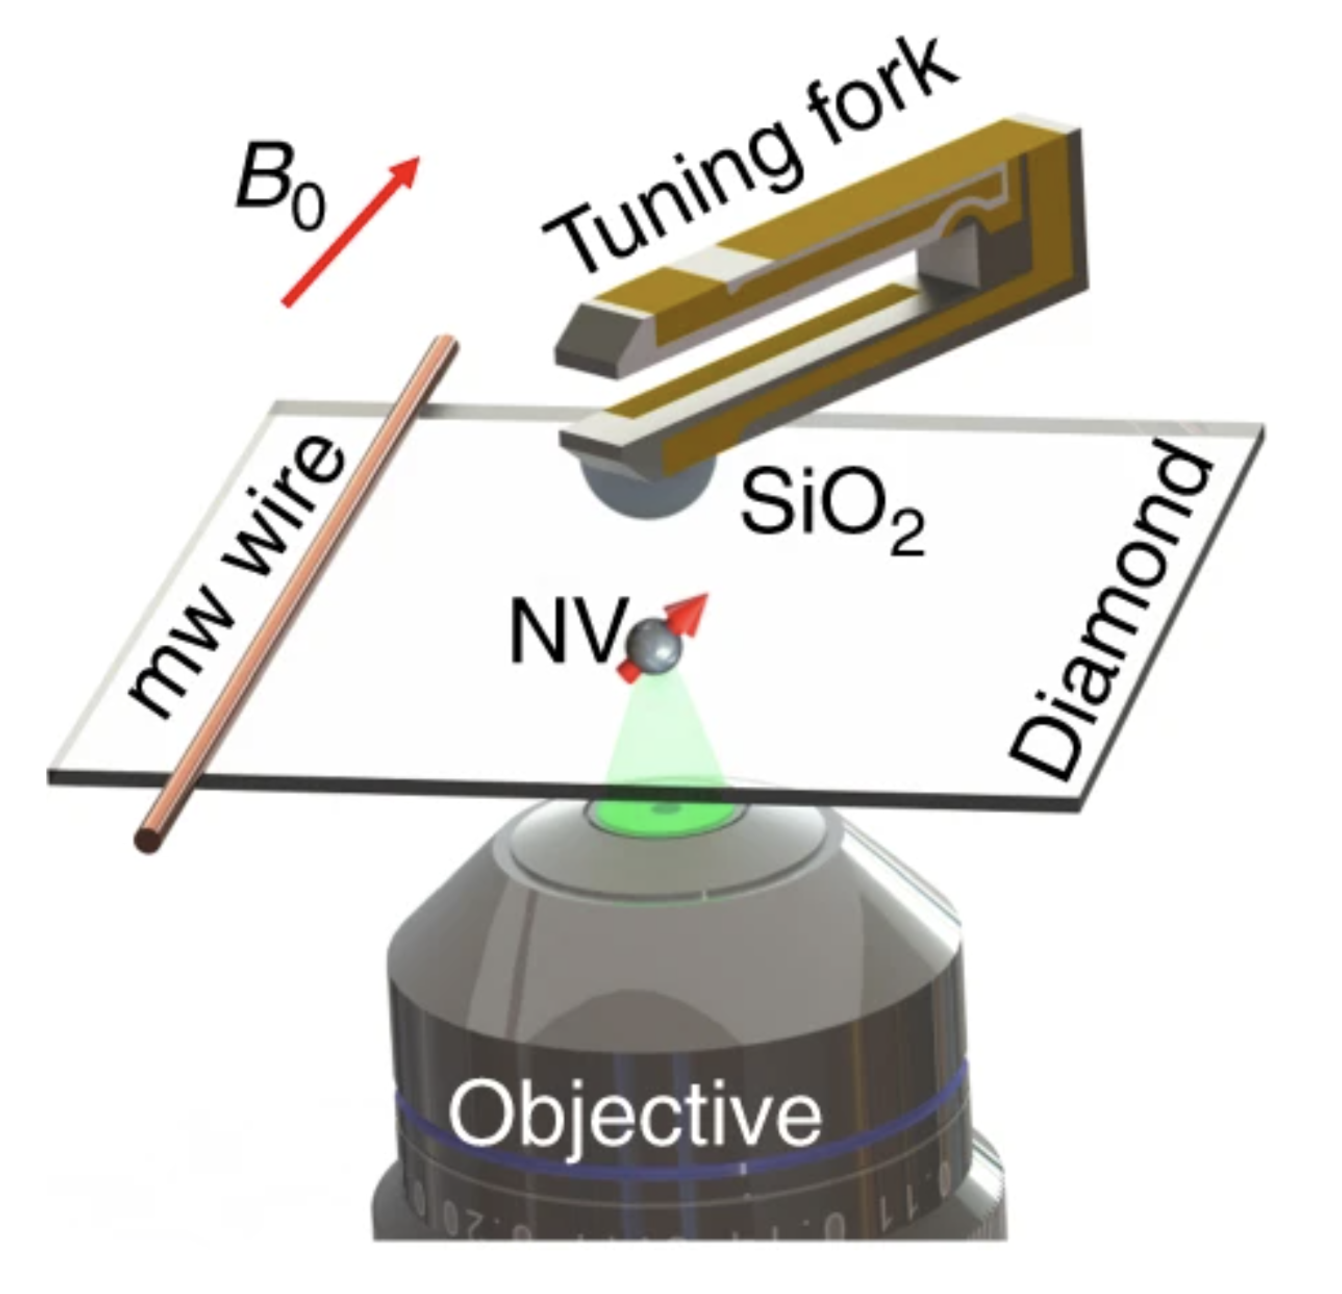
\includegraphics[width=0.3\textwidth]{Fig6.eps}
\end{center}
\caption{NV-diamond magnetometer setup used by \citet{rong_searching_2018}. 
From top to bottom: 
The source is a $\rm SiO_2$ hemisphere, which is driven to oscillate vertically by a tuning fork, thereby modulating the exotic force. 
The sensor is an NV magnetometer on a diamond rectangular plate. %plate-shaped diamond. 
The NV center is pumped with a green laser and emits red fluorescent light, which is collected via the same objective that delivers the pump light. 
A wire is used to deliver microwaves to the NV center driving a transition between two Zeemann levels. 
The direction of the source movement can be changed to search for different types of exotic interactions 
(\citealp{rong_searching_2018}, \citeyear{rong_observation_2020}; \citealp{jiao_experimental_2021}; \citealp{liang_new_2022}).
%\cite{rong_searching_2018,rong_observation_2020,jiao_experimental_2021,liang_new_2022}.
} \label{nvexperimentsetup}
\end{figure}
%\Haosen{Haosen:
One typical experiment using an NV-based sensor \cite{rong_searching_2018} is shown in Fig.\,\ref{nvexperimentsetup}. 
%a mass source composed of a semispherical SiO$_2$ is attached on a tuning fork of AFM and driven to oscillate vertically. The single NV center below the mass source is used to detect the spin-dependent interaction induced by the mass source. The objective lens is used to focus the laser on the single NV center and at the same time collect the fluorescence emitted by the NV center. 
A $\rm SiO_2$ hemisphere is utilized as an unpolarized mass source (see Sec.\,\ref{METH1.SOUR.}), which is driven to oscillate in the vertical direction, thereby tuning the relative velocity and the distance from the source to the sensor. 
As a result, an otherwise static exotic interaction can be modulated into a sinusoidal signal in the kHz frequency range.
A spin-echo protocol \cite{rong_searching_2018} or continuous-wave protocol \cite{liang_new_2022} can be used to detect the oscillating pseudo-magnetic field. 

In another experiment \cite{rong_constraints_2018}, a laser-pumped single crystal of $p$-terphenyl-doped pentacene-$d_{14}$ is used as a source of polarized electron spins. 
%The advantage of using a single-NV sensor is the size is small in comparison with the force range, so the sensor can be positioned close enough to the source to avoid the drop of the potential with distance. 
%Such a geometry enables close proximity between the sensor and the source. 
The NV sensor experiences an effective magnetic field induced by polarized electrons, resulting from the coupling between the two systems, including the magnetic dipole-dipole interaction and an exotic axial-vector dipole-dipole interaction, 
%\YS{
with the magnetic dipole-dipole interaction given by 
\begin{equation}
H=-\frac{\mu_0\gamma_e\gamma_e\hbar^2}{(16\pi r^3)}[3(\boldsymbol{\sigma}_e \cdot \hat{\boldsymbol{r}})(\boldsymbol{\sigma}_e^{\,\prime} \cdot \hat{\boldsymbol{r}})-\boldsymbol{\sigma}_e \cdot \boldsymbol{\sigma}_e^{\,\prime}]\,,
\end{equation}
%where the indices $1,2$ denote the two electrons.
%} 
where $\mu_0$ is the magnetic constant (permeability of free space). The authors selected a single-NV center in their sample and measured the overall coupling strength to the polarized-electron source using a pulse sequence that measures the phase shift between NV sublevels that results from spin-spin interactions. 
This phase shift is then converted to the population of the NV-center $\ket{m_s=0}$ state and measured. 
The experiment was repeated for three single-NV centers at different locations with respect to the source. 
Based on a fitting of their data to the phase shift caused by the effective magnetic field %\DB{We need to check the factors of 2 here}
\begin{align}
&b_\textrm{eff}(r,\theta)=\nonumber\\&-\frac{\mu_0 \gamma_e \hbar}{(8\pi r^3)} \times [3{\cos}^2(\theta)-1] + {g_A^eg_A^e} \frac{e^{-\frac{r}{\lambda}}} {({2\pi \hbar \gamma_e r})}\,,
\end{align}
\citet{rong_constraints_2018} obtained an upper limit on the exotic axial-vector dipole-dipole interaction constant product $g_A^eg_A^e$, which was treated as a fitting parameter. 

An outlook towards future NV-based experiments is given by \citet{chu_proposal_2022} and \citet{du_single-molecule_2024}. For further discussion, see Sec.\,\ref{Sec:limits_main}.

%There's also a new proposal to use a diamond-based vector magnetometer with ensembles of nitrogen-vacancy centers along different axes in a diamond, described in \citet{guo_searching_2024}. \LC{It has been mentioned in the end of Sec.\,\ref{subsec_g_Ag_A}.}
%\url{https://arxiv.org/abs/2402.15042}.



%The sensitivity of the NV experiment can be further enhanced, see \citet{chu_proposal_2022}.



%%%%%%%%%%%%%%%%%%%%%%%%%%%%%%%%%%%%%%%%%%%%%%%%%%%%%%
                      % S4. CN
%%%%%%%%%%%%%%%%%%%%%%%%%%%%%%%%%%%%%%%%%%%%%%%%%%%%%%


\subsubsection{Particle beams}
\label{METH1.SENS.PBS}

Beyond the spin-based sensors mentioned previously,
an extensive array of other spin-based sensors are employed or suggested for the exploration of exotic spin-dependent interactions. These include particle beam sensors
(\citealp{piegsa_limits_2012}; \citealp{yan_new_2013}; \citealp{schulthess_new_2022}; \citealp{snow_searches_2022}).
%\cite{piegsa_limits_2012, yan_new_2013, schulthess_new_2022, snow_searches_2022}.
%\DK{add reference} \YS{Some possible suggestions include:  levitated ferromagnetic torque sensors \cite{jackson_kimball_precessing_2016,vinante_surpassing_2021,ahrens_levitated_2024} \DK{weren't these mentioned previously?} \YS{I think that's correct, though I'm not sure what levitated ferromagnetic sensors and the following two magnetometry methods have to do with particle beams -- I think the two magnetometry methods mentioned here may fit better in the subsection \ref{METH1.SENS.AM} on co-magnetometry.}, atomic Bose-Einstein condensate magnetometers \cite{rosenband_observation_2007},
%\DK{add reference: Vengalattore, M., et al. ``High-resolution magnetometry with a spinor Bose-Einstein condensate." Physical review letters 98.20 (2007): 200801.}, 
%and liquid-state nuclear comagnetometers \cite{wu_nuclear-spin_2018}, among others. 
Certain particle beam sensors, such as muon and neutron beams, show sensitivity to the interactions of exotic fields. Moreover, some beams are tailored for specific objectives, for instance, neutron beams are deployed in experiments aimed at discovering a permanent neutron electric dipole moment (EDM) \cite{abel_measurement_2020}. 

%%%%
%\paragraph{Cold and ultracold neutrons}
%Polarized cold neutrons can be sensitive to exotic interactions.

Having no electric charge and other advantageous properties such as their small polarizability, neutrons are an attractive system for fundamental experiments. In fact, 
cold and ultracold neutrons have been used as probes for various exotic interactions as discussed in comprehensive reviews by \citet{sponar_tests_2021} and \citet{snow_searches_2022}.
Polarized beams of slow neutrons with energies below $0.025$\,eV propagating through liquid $^4$He have been used to search for potential new interactions over mesoscopic distances.
%\YS{Should we give a reference(s) here?} 
For example, experiments have established an upper limit on the strength of possible long-range $P$-odd interactions between neutrons and both nucleons and electrons, derived from data on the search for parity violation in neutron spin-rotation within liquid $^4$He \cite{yan_new_2013}. 
% Furthermore, ultracold neutrons \DB{Add energy} are being applied in the searches for the neutron EDM.
Experiments involving ultracold neutrons with energies below $10^{-7}$\,eV (and $^{199}$Hg atoms as a comagnetometer) have been used to probe axionlike dark matter \cite{abel_search_2017} and search for a permanent EDM of the neutron \cite{abel_measurement_2020}. 
Applying a strong electric field allowed placing new limits on the coupling of axion dark matter to gluons, achieved using a Ramsey-type apparatus designed for cold neutrons \cite{schulthess_new_2022}.
Other current and proposed neutron-based experiments could open new avenues for the exploration of exotic interactions 
(\citealp{nesvizhevsky_quantum_2002}, \citeyear{nesvizhevsky_neutron_2008}; \citealp{baesler_constraint_2007}; \citealp{pokotilovski_neutron_2011}; \citealp{piegsa_proposed_2012}; \citealp{cronenberg_gravity_2015}; \citealp{haddock_search_2018}; \citealp{fujiie_development_2024}). 
%\citet{baesler_constraint_2007,pokotilovski_neutron_2011,piegsa_proposed_2012,haddock_search_2018,fujiie_development_2024,nesvizhevsky_neutron_2008,voronin_search_2023,nesvizhevsky_quantum_2002,cronenberg_gravity_2015}. 
A summary of existing neutron beam experiments that search for spin-dependent exotic interactions is given in Sec.\,\ref{subsec_g_Pg_S_n-N}. 

% \YS{I don't know if it's entirely relevant here, but
% a somewhat different (non-purely-``atomic'') comagnetometer using atomic mercury and ultracold neutrons has been used to search for dark matter \cite{abel_search_2017} and to search for a permanent EDM of the neutron \cite{abel_measurement_2020}. We discuss free neutrons as sources in Sec.~\ref{METH1.SOUR.NSS} and there's a plan to discuss neutrons in the context of particle beam sensors in Sec.~\ref{METH1.SENS.PBS}, though I'm not aware of discussion of ultracold neutrons in the context of sensors (i.e., ultracold neutrons stored in a chamber) in Sec.~\ref{METH1.SENS.}. Are there plans for such discussion?} \footnote{\YS{This assumes that the different species are co-located and at the same temperature. In the case of, e.g., a comagnetometer consisting of ultracold neutrons and warmer mercury atoms occupying the same volume, the C.M. of the neutrons is at a slightly lower height than that of the mercury atoms due to Earth's gravity, and so the comagnetometer becomes sensitive to gradients in magnetic fields.}}

%A review — \cite{cronenberg_gravity_2015} Harmut Abele,  Gravity of Earth Measurement with a qBOUNCE Experiment  

%\LC{Two papers Dima mentioned \cite{bosina_qbounce_2023,sponar_tests_2021} about qBOUNCE.}

%\YS{There's an overview of searches for exotic forces with neutron beam experiments in \citet{snow_searches_2022}.
%\url{https://www.mdpi.com/2073-8994/14/1/10}. Another (proposed) experiment is called GRANIT. From memory, many of these experiments search for spin-independent forces, but there are spin-dependent variations; e.g., in \citet{baesler_constraint_2007,pokotilovski_neutron_2011,piegsa_proposed_2012,haddock_search_2018}.
%\url{https://journals.aps.org/prd/abstract/10.1103/PhysRevD.75.075006}, \url{https://link.springer.com/article/10.1134/S0021364011180111}, \url{https://iopscience.iop.org/article/10.1088/1742-6596/340/1/012043/meta}, \url{https://www.sciencedirect.com/science/article/pii/S0370269318305227}.  Dima mentions the novel neutron-beam interferometer in \citet{fujiie_development_2024}.
%\url{https://journals.aps.org/prl/abstract/10.1103/PhysRevLett.132.023402}.  If we're discussing neutron-beam experiments here, then another pioneering experiment to mention is \citet{nesvizhevsky_quantum_2002}
%\url{https://www.nature.com/articles/415297a#author-information} 

%(there's a separate paper searching for spin-independent interactions by at least one of the same authors in \cite{nesvizhevsky_neutron_2008}).}

%\LC{YS:A reference for spin-independent \cite{voronin_search_2023}. }


%\paragraph{Other spin-based sensors}
%\label{METH1.SENS.Other}

%Some liquid-state NMR sensors are not discussed here, some ideas of these sensor are similar to that of atomic magnetometer.
%For instance liquid-state NMR comagnetometer is mentioned in the atomic magnetometer.
%There are some liquid state nuclear spin based sensor, for instance, the liquid Xe sensor used in CASPEr experiment is essentially spin polarized atomic spin sensors that are further liquefied and detected by SQUID sensor.
%\YS{Are there plans to expand on this section?} 
%\YS{It looks like we don't define the acronym NMR in the main text until later on in this review. The term appears earlier in Table~\ref{tabel_sensor} (currently undefined there).} \LC{It has been defined ealier in sec.\,\ref{METH1.SENS.AM.SMSA}.}



%\subsection{Other techniques}
%\label{METH1.SENS.OT}
%%%%%%%%%%%%%%%%%%%%%%%%%%%%%%%%%%%%%%%%%%%%%%%%%%%%%%
                      % METH1.recipe
%%%%%%%%%%%%%%%%%%%%%%%%%%%%%%%%%%%%%%%%%%%%%%%%%%%%%%
%\subsection{Designing a dedicated exotic force search -- a recipe}
%\label{METH1.REC.}
%1, find your fermion spin and estimate the spin density. Maybe you can refer to Table\ref{tabel_source}. Find which term of coupling you are sensitive to, by refering to \ref{tabel_f-gg}. Design your experiment.
%%%
\iffalse
\begin{figure} [!htbp]
\begin{center}
\includegraphics[width=0.55\textwidth]{experiments6.png}
\end{center}
\caption{A conceptual setup for experiments searching for spin-dependent fifth forces. 
\LC{Is this figure useful or do we need to change it to fit our needs?} 
\YS{I think this figure (or a slightly modified variant) would be a nice inclusion at the start of this chapter in Sec.\,\ref{Sec:source-sensor_general_remarks} to illustrate the basic setup in spin-dependent fifth-force searches. 
One thing's that's not clear to me is whether the label ``Exotic field'' refers to the exotic field at the position of the spin sensor, or the magnetic field induced by the spin sensor as a result of its interaction with the spin source, or represents the field of the exchanged boson ($Z'$ in this case) - it is possible to clarify this in the diagram? 
Regarding the main text here in Sec.\,\ref{METH1.REC.}, (some of) this material could be useful in the introductory part Sec.\,\ref{Sec:source-sensor_general_remarks}, e.g., if we want to discuss general features of experiments and refer to tables in this chapter (for ease of reference).}} 
\label{Fig:experimental_setup_spin_force}
\end{figure}
\fi
%%%%%%%%%%%%%%%%%%%%%%%%%%%%%%%%%%%%%%%%%%%%%%%%%%%%%%
               % Sec-Complementary Method
%%%%%%%%%%%%%%%%%%%%%%%%%%%%%%%%%%%%%%%%%%%%%%%%%%%%%%

%%%%%%%%%%%%%%%%%%%%%%%%%%%%%%%%%%%%%%%%%%%%%%%%%%%%%%
                      % Me2. (Method2)
%%%%%%%%%%%%%%%%%%%%%%%%%%%%%%%%%%%%%%%%%%%%%%%%%%%%%%
\section{Complementary experiments and observations to detect exotic spin-dependent interactions}\label{EXP.METH.2}
\subsection{General remarks }

%\LC{Read Sec. I. C. of \citet{safronova_search_2018}.}
In addition to the source-sensor experiments discussed in Sec.\,\ref{Sec:EXP.METH.1}, various other experiments, not necessarily initially dedicated to searching for fifth forces, can be used to search for such forces, as we discuss here. 
Among such precision measurements at subatomic, atomic, and molecular scales are experiments related to high-precision spectroscopy of various exotic atoms, parity violation, searches for EDMs, isotope shifts ad so on. 

In analyzing such experiments, it should be recognized that, while the range of an interaction is given by the inverse mass of the intermediate boson responsible for the interaction, the effects of the interaction can be observable on much larger scales. 
An example of such a ``cascade of scales'' is the spin-dependent atomic parity violation effect due to the nuclear anapole moment (Sec.\,\ref{METH2.PV}). 
Indeed, weak interactions are mediated by $W$ and $Z$ bosons, the masses of which (80 and 91\,GeV/$c^2$, respectively) correspond to an interaction range of $\sim 10^{-16}$\,cm, which is much smaller than the nuclear size (between 10$^{-13}$ and 10$^{-12}$\,cm). However, the 
%(parity-conserving) 
exchange of mesons withing the nucleus ``spreads'' the influence of parity nonconservation (PNC) interactions over the entire nucleus, generating a parity-violating anapole moment. 
The presence of the nuclear anapole moment in turn affects the atomic electrons and can be (and indeed was) detected in atomic experiments. 


%One also needs to be careful about how the effects of the weak and strong forces may manifest in precision measurement experiments. 
% For instance, the Z boson has a mass corresponding to an interaction range of $10^{-16}$ cm or so. 
% However, we can observe the effect in atoms. 
% This teaches us a lesson that, sometimes, an exotic interaction can manifest at a much larger spatial scale than the inverse mass of the carrier. \DK{This seems a bit of strange formulation, because the point in PV experiments is that the electron wavefunction is affected by short-range parity-violating forces precisely becuase its wavefunction penetrates into the nucleus. Perhaps re-phrase in terms of the concept that extremely short range forces can generate effects on much larger composite systems?}
%\DB{Note also that this how PV interactions propagate in nuclei---a diagram with one PV vertex and one PC vertex}
%%%%%%%%%%%%%%%%%%%%%%%%%%%%%%%%%%%%%%%%%%%%%%%%%%%%%%
                      % Me2.PM
%%%%%%%%%%%%%%%%%%%%%%%%%%%%%%%%%%%%%%%%%%%%%%%%%%%%%%
\subsection{Precision measurements}
\label{METH2.PM}
%\WJ{I put this here temporarily, this was in the first paragratph of section \ref{METH1.SENS.}}画
%\YS{I propose adding the word ``ideally'' in the previous sentence, since it is in principle possible for systems with zero net spin to be sensitive to spin-dependent forces at higher order. For example, a suitably chosen linear combination of states with angular-momentum projections $m_F = \pm 1$ is insensitive to the first-order Zeeman shift but is sensitive to the second-order Zeeman shift. Atomic clock spectroscopy experiments often use this approach to strongly suppress systematic effects associated with stray magnetic fields. Maybe we could discuss this point somewhere?} \WJ{Very good point, what about we mention this in the experiment-theory comparison experiments? } \YS{This would be good - maybe we could discuss this in one of the subsections on atomic spectroscopy?}
%{\color{red}YS: Is this discussion still needed? It looks like we're missing some of the context here.} 



%%%%
\subsubsection{Trapped ions     }
\label{METH2.PM.TI}

Trapped ions have been extensively studied for their applications in precision measurements \cite{cairncross_precision_2017,blaum_high-accuracy_2006}, quantum computing (\citealp{cirac_quantum_1995}; \citealp{blatt_entangled_2008}; \citealp{harty_high-fidelity_2014}; \citealp{bruzewicz_trapped-ion_2019})
%\cite{cirac_quantum_1995,harty_high-fidelity_2014,blatt_entangled_2008,bruzewicz_trapped-ion_2019}
and quantum simulation 
(\citealp{blatt_quantum_2012}; \citealp{lv_quantum_2018}; \citealp{cong_selective_2020}; \citealp{monroe_programmable_2021}).
%\cite{blatt_quantum_2012,lv_quantum_2018,cong_selective_2020,monroe_programmable_2021}. 
Precision measurements using trapped ions refer to the use of ion traps and precise ion control to make accurate measurements of various physical quantities, with applications in tests of fundamental physics 
(\citealp{wineland_search_1991}; \citealp{kotler_constraints_2015}; \citealp{cairncross_precision_2017}),
%\cite{wineland_search_1991,cairncross_precision_2017,kotler_constraints_2015},
atomic clocks 
(\citealp{rosenband_frequency_2008}; \citealp{ludlow_optical_2015}; \citealp{kozlov_highly_2018}; \citealp{safronova_search_2019}; \citealp{burt_demonstration_2021}),
%\cite{safronova_search_2019,ludlow_optical_2015,kozlov_highly_2018,rosenband_frequency_2008,burt_demonstration_2021}, 
and more. 

\citet{wineland_search_1991} searched for an exotic dipole-monopole interaction by examining the hyperfine resonances of approximately 5000 trapped and cooled $^9$Be$^+$ ions. The nucleons in the Earth served as the source, while the ions acted as a spin sensor. An applied magnetic field was switched between being directed either parallel or antiparallel to the direction of gravity, and any contribution of the exotic interaction would be revealed by a difference in the resonance frequency of the transition between the $^2 S_{1/2} \ket{F=1,M=0}$ and $^2 S_{1/2} \ket{F=1,M=-1}$ states of the $^9$Be$^+$ ions. Additionally, \citet{wineland_search_1991} studied the dipole-dipole interaction with the same ions, using electron spins in an electromagnet as the dipole source. 

Experiments involving ion traps can also detect small deviations from the predictions of established physical theories, potentially leading to discovery of new physics beyond the SM. \citet{kotler_measurement_2014} confined two ions of $^{88}$Sr$^+$ at a separation of one micrometer using a linear radio-frequency Paul trap. The ions evolved under the magnetic dipole-dipole interaction and reached a final state that encoded information about the strength of the interaction, which could be determined by interrogating the ions. This technique enabled precise measurement of the magnetic dipole-dipole interaction between the ions.
\citet{kotler_constraints_2015} compared their experimental result \cite{kotler_measurement_2014} on the strength of the interaction to a theoretical calculation: the small uncertainty was translated into new constraints on the strength of an axial-vector- or pseudoscalar-mediated interaction between electrons. 

The work of \citet{wineland_search_1991} and \citet{kotler_constraints_2015} emphasized trapped and cooled ions as a useful platform for exotic interaction searches, benefiting from the controllability of trapped ions and the relatively straightforward analysis of systematic errors.


%\LCa{Need rewrite and maybe a little bit longer content. Copy from \citet{safronova_search_2018}.}
%Between a $\mu$m and a mm, the best direct constraint on axial-vector dipole-dipole interactions between electrons comes from the measurement of the magnetic dipole-dipole interaction between two trapped $^{88}$Sr$^+$ ions \cite{kotler_measurement_2014,kotler_constraints_2015}. \citet{kotler_measurement_2014} trapped two $^{88}$Sr$^+$ ions using a linear radio-frequency Paul trap, and the ions were initialized in an entangled state that was insensitive to spatially homogeneous magnetic field noise. This technique enabled precise measurement of the magnetic dipole-dipole interaction between the ions, which when compared to a straightforward calculation gave good agreement at a level of $\approx 200~{\rm \mu Hz}$. \citet{kotler_constraints_2015} then used the agreement between experiment and theory to limit the strength of exotic dipole-dipole interactions. \LCa{Even though later the result has been surpassed by \citet{ficek_constraints_2017,fadeev_pseudovector_2022} thorough investigation of the electronic structure of $^4$He and \citet{yan_constraining_2019} using electron g-factor, trapped ions still represents an frontier research method.}

\subsubsection{Atomic spectroscopy }\label{METH2.PM.AHS}
%\subsubsection{Atomic and molecular precision spectroscopy- Misha}\label{METH.PM.PS}

Spectroscopic experiments are arguably the most accurate experiments in physics. 
The relative inaccuracy of a routine spectroscopic experiment is about $10^{-8}$, or better, while the best atomic clocks have a fractional inaccuracy on the order of $10^{-19}$. 
This accuracy corresponds to potentially high sensitivity to exotic interactions, provided that there is a theoretical standard-model prediction for the observed transition of a comparable accuracy. 
At present, this is possible only for a limited number of simple systems (\citealp{karshenboim_hyperfine_2011,karshenboim_constraints_2010,karshenboim_precision_2010}; \citealp{ficek_constraints_2017}; \citealp{ficek_constraints_2018}) which consist of only a few particles and ideally lack hadronic particles.
%\cite{ficek_constraints_2017,ficek_constraints_2018}.\LC{is it ok to cite them here?}
%\YS{I don't recall this point being made in these two papers. These papers discuss simple systems containing helium nuclei. Maybe there are better reference(s) to support the point being made in the text?} \LC{Dear Pasha, could you have a look here.}
%\PF{We look at table 1 of 2017 and table 1 of 2018, and we see that the theoretical and experimental uncertainties are not of the same order of magnitudes, so these may not be the best example of comparable accuracy.}
(As discussed in Sec.\,\ref{Sec:Intro-Exp}, this applies to searches that rely on theory-experiment comparisons; high experimental precision alone may be sufficient for searches that do not strongly rely on highly accurate theory.) 

Even in the case of hydrogen, the accuracy of the theory is limited by the fact that the proton is not an elementary particle, but rather is a hadronic state consisting of quarks bound together via their interactions with gluons. 
One way to bypass this limitation is to look at the difference of the effect for different quantum numbers (\citealp{karshenboim_precision_2010}; \citealp{fadeev_pseudovector_2022}). 
For example, the hyperfine splitting $\Delta_\mathrm{hf}(n)$ of the $s$-states scales with the principal quantum number $n$ as $\propto 1/n^3$. Therefore, one can look, for example, for the difference $\Delta_{21}=8\Delta_\mathrm{hf}(2s)-\Delta_\mathrm{hf}(1s)$. Exotic spin-spin interactions, which decrease with the distance as $1/r$ rather than $1/r^3$, scale differently with $n$ and contribute to the nonzero $\Delta_{21}$.\footnote{There are also residual contributions to $\Delta_{21}$ from nuclear structure and other standard-model effects \cite{karshenboim_hyperfine_2002,karshenboim_hyperfine_2002-1,yerokhin_electron_2008}.} 


\subsubsection{Spectroscopy of exotic atoms }\label{METH2.PM.EA}
%\subsubsection{Exotic atoms -Filip}

Fine structure in simple atoms is less sensitive to the nuclear size and can be calculated more accurately. 
This allows direct comparison of the theoretical prediction with the experiment. 
The most accurate calculations of the fine structure are possible for systems such as positronium and muonium, which are devoid of on-shell hadronic particles.

Exotic atoms incorporate particles other than the common protons, neutrons, and electrons. 
The simplest examples include positronium, which is a bound state of a positron and an electron, or muonium -- a bound state of an antimuon and electron. 
Their simplicity and the fact that they contain unusual components make them an ideal laboratory for fundamental physics. 
Comparison of theoretical calculations and experimental measurements for various transitions in such systems has led to constraints on interactions between the constituents of positronium (\citealp{frugiuele_current_2019}; \citealp{fadeev_pseudovector_2022})
%\cite{fadeev_pseudovector_2022, frugiuele_current_2019} 
and muonium (\citealp{frugiuele_current_2019}, \citeyear{frugiuele_muonic_2022}; \citealp{ohayon_precision_2022}; \citealp{fadeev_pseudovector_2022}).
%\cite{fadeev_pseudovector_2022, frugiuele_current_2019,frugiuele_muonic_2022,ohayon_precision_2022}. 

Simple atoms and molecules may be used to test theories with extra dimensions which predict highly singular gravitational forces on short length scales; see, for example, \citet{arkanihamed_hierarchy_1998} and \citet{arkani-hamed_phenomenology_1999}. Limits on the size and number of extra dimensions have been obtained by \citet{salumbides_constraints_2015} and \citet{dzuba_effects_2022}.

A more complicated exotic atom is antiprotonic helium. 
It is an atomic system consisting of an electron and an antiproton orbiting around a helium nucleus \cite{yamazaki_antiprotonic_2002}. 
Such atoms are usually produced by slowing down antiprotons in a helium environment, leading to the replacement of one of the electrons in a He atom. 
Of the resulting atoms, a small fraction have antiprotons in orbits with quantum numbers $(n,l)=(38,37)$, giving metastable states with lifetimes on the order of microseconds. 
%\YS{Are these Rydberg states in the usual sense? If they are, then maybe worth describing the orbits as Rydberg or Rydberg-like orbits.} \LC{Dear Filip, could you take a look?} \FF{These are Rydberg states in the sense that the antiproton is highly excited, but I believe they lack typical properties of Rydberg states since the orbiting particles are at comparable distances from the nucleus.} \YS{Thank you for clarifying, Filip!}
These states were used for measurements of various antiproton properties, such as its magnetic moment (\citealp{pask_antiproton_2009}; \citealp{nagahama_sixfold_2017}; \citealp{smorra_parts-per-billion_2017})
%\cite{pask_antiproton_2009, nagahama_sixfold_2017, smorra_parts-per-billion_2017}
and mass \cite{hori_buffer-gas_2016}. 
As such, antiprotonic helium plays an important role in testing $CPT$ invariance \cite{hayano_antiprotonic_2007}. 

Antiprotonic-helium spectroscopy has yielded the first constraints on semileptonic spin-dependent interactions between matter and antimatter. \citet{ficek_constraints_2018} compared the experimental measurements of transition energies between two states within the hyperfine structure (hfs) of the antiprotonic helium $(n,l)=(37,35)$ state \cite{pask_antiproton_2009} with quantum electrodynamics (QED) based predictions \cite{korobov_fine_2001}. 
This led to constraints on several types of exotic interactions between an electron and an antiproton, including higher-order velocity-dependent interactions. 

At present, there is good agreement between theory and experiment for the fine structure of normal and exotic atoms, which can be used to constrain exotic spin-dependent interactions at distances on the order of a Bohr radius (and greater). 

%\subsubsection{Molecular spectroscopy (need reorganize)}\label{METH2.PM.MS}




%\LC{Atomic or molecular spectroscopy references: \cite{fadeev_pseudovector_2022,ficek_constraints_2018,ficek_constraints_2017, ledbetter_constraints_2013,jackson_kimball_constraints_2010,ramsey_tensor_1979}.}

\subsubsection{Nuclear magnetic resonance    }\label{METH2.PM.NMR}

Similarly to the case of precision atomic and molecular spectroscopy, high-precision NMR measurements can also be sensitive to spin-dependent exotic forces. One can illustrate this with the measurement of spin-spin coupling in the isotopologues of the hydrogen dimer, e.g., HD \cite{ledbetter_constraints_2013}.

% Nuclear spins in molecules interact with each other as magnetic dipoles. This interaction is sensitive to the orientation of the molecule and averages to zero for liquid or gas samples. 
The conventional dipole-dipole interactions between nuclear spins are averaged in liquid and gas samples as a result of rapid (on the time scale given by the strength of the interaction) tumbling of molecules. However, spin-spin interactions are still present (\citealp{hahn_chemical_1951}; \citealp{gutowsky_nuclear_1953})
%\cite{hahn_chemical_1951,gutowsky_nuclear_1953} 
due to second-order hyperfine interaction \cite{ramsey_interactions_1952}: the interaction with a nuclear spin perturbs the electronic wavefunction of the molecule, and this perturbation is ``carried'' by the electrons to the second nucleus, which ``feels'' this perturbation, once again, due to the hyperfine interactions. This interaction of the form $J\,\bm{I}_1\cdot\bm{I}_2$ (where \textit{J} is the interaction strength) and is often referred to as scalar or \textit{J}-coupling. For simple molecules such as hydrogen, \textit{J}-couplings can be accurately calculated and a comparison between the experimental and theoretical result may reveal the presence of an exotic force.

Although the early analysis \cite{ledbetter_constraints_2013} of the existing data and calculations produced upper limits on the strength of exotic interactions, the experimental work of \citet{neronov_nmr_1975}; \citet{neronov_determination_2014}; \citet{ garbacz_indirect_2016}; \citet{neronov_determination_2018} actually claimed a significant disagreement with theory and a possible discovery of a pseodoscalar boson (an axion with a mass in the vicinity of 1\,keV). However, subsequent theoretical work \cite{puchalski_nuclear_2018} considered nonadiabatic corrections ignored in the earlier theory and brought the experiment and theory into agreement with each other.

%Using the improved experimental \cite{neronov_determination_2018} and theoretical \cite{puchalski_nuclear_2018} results, we can improve on the earlier constraints by \citet{ledbetter_constraints_2013} and obtain... \LC{add a link to our arxiv note}

%\DB{A request to Lei: is there a possible improvement on the analysis from Ledbetter et al that can be made here...? Please ask Derek to read this and then maybe also Pachucki ?} \LC{\citet{ledbetter_constraints_2013} compared the averaged theory and experimental results from several works and obtained that the agreement between theory and experiment is $\Delta$J=0.003, however, \cite{puchalski_nuclear_2018}'s result gives $\Delta$J=0.0242 compared to the averaged experiment result. This value may be further reduced by take the finite nuclear mass effects into consideration. However, perhaps \cite{puchalski_nuclear_2018}'s theory result will not significantly improve the constraints? Anyway, it worth to look deeper into \cite{puchalski_nuclear_2018} as they also calculated HT and DT.}

%\LCa{so Dima's opinion is the $\Delta_E$ is not only decised by the average difference, but also by the uncertainty, one should use the Eq.\,(A1) and (A2) in \cite{ficek_constraints_2017}.}
%\DB{Actually, Misha writes:} 
%The agreement is not perfect, but discrepancies can be caused by the temperature-dependent and non-adiabatic effects, which are not yet fully included in the theory. 
%\DB{So we need to figure out if there is agreement or not...}
%\MK{I would say, that there is no contradiction.}
 
% For the hydrogen molecule and its isotopologues, such as HD and HT, the $J$-coupling splitting can be calculated accurately \cite{puchalski_nuclear_2018} and compared with respective measurements \cite{neronov_nmr_1975, neronov_determination_2015, garbacz_indirect_2016}. 
% %[Neronov, Barzakh, Mukhamadiev, JETP, v.42, 950 (1975); Neronov and Seregin, JETP-Lett. v.100, 609 (2015), P. Garbacz, M. Chotkowski, Z. Rogulski, and M. Jaszuński, J. Phys. Chem. A 120, 5549 (2016)] 
% The agreement is not perfect, but discrepancies can be caused by the temperature-dependent and non-adiabatic effects, which are not yet fully included in the theory.




%%%%%%%%%%%%%%%%%%%%%%%%%%%%%%%%%%%%%%%%%%%%%%%%%%%%%%
                      % Me2.APV
%%%%%%%%%%%%%%%%%%%%%%%%%%%%%%%%%%%%%%%%%%%%%%%%%%%%%%

\subsection{Atomic and molecular parity-violation experiments    }
\label{METH2.PV}
%\LCa{Content from the introduction:}

\subsubsection{Atomic parity violation} 
\label{METH2.PV.APV}
%One example of spin-dependent interactions is that of an electron-nucleus interaction resulting in atomic parity violation (APV; \citet{safronova_search_2018}). 
%\LC{new: 
\citet{safronova_search_2018} [see also \citet{kawasaki_nuclear_2024}] reviewed spin-dependent interactions based on an electron-nucleus interaction resulting in atomic parity violation (APV). %}
In the nonrelativistic limit, the parity-violating term in the Hamiltonian is proportional to $\v{s} \cdot \v {p}$, where $\v{s}$ is the electron or nuclear spin and $\v{p}$ is the electron momentum. 
The APV effect is due to the exchange of a $Z$ boson that was predicted by the Weinberg-Salam electroweak theory. Observation of APV by \citet{barkov_observation_1978} played an important role in establishing the SM.   
%,antypas_measurement_2014}. 
%on the  effective energy range of,  a very imporytnat role in establishing nthenStandard Mod
%\YS{I'm not sure what's meant here - the sentence seems incomplete, and also there's no $Z'$ boson in the standard model - there's only a $Z$ boson}
This is an excellent example showing that precision measurements conducted at low energies can provide an alternative way of exploring high-energy physics, apart from the fruitful but expensive accelerator-based experiments and astrophysical observations. 

Weak neutral currents in the standard model arise from the exchange of a heavy $Z$-bozon. 
On the atomic scale, it corresponds to a short-range interaction. 
This leads to a strong $Z$-dependence of parity violation (PV) effects. 
For neutral atoms, the dominant nuclear-spin-independent PV effects scale with the nuclear charge $Z$ faster than $\propto Z^3$ \cite{bouchiat_i_1974,bouchiat_parity_1975}. 
Because of this scaling, most APV experiments have been performed on heavy atoms. 
At present, APV has been observed in Bi \cite{barkov_observation_1978}, Pb \cite{meekhof_high-precision_1993}, Tl \cite{edwards_precise_1995,vetter_precise_1995}, Cs \cite{wood_measurement_1997}, and Yb \cite{tsigutkin_observation_2009}. 
%\YS{Maybe we could cite the first successful measurements in each of these atomic species?} \LC{added, please check.} \YS{Thank you for adding the references! Just a question about formatting: the added references appear to have a different format in the bibliography (e.g., there is the DOI, but the journal details appear to be missing). Is it possible to update these entries?} 
All observed effects are in agreement with the predictions of the SM. 
The most accurate measurement \cite{wood_measurement_1997} and theoretical calculations 
(\citealp{dzuba_relativistic_1985}, \citeyear{dzuba_summation_1989}, \citeyear{dzuba_summation_1989-2}, \citeyear{dzuba_summation_1989-1}, \citeyear{dzuba_high-precision_2002}, \citeyear{dzuba_long-range_2022}; \citealp{blundell_high-accuracy_1990}; \citealp{flambaum_radiative_2005}; \citealp{porsev_precision_2009}; \citealp{sahoo_new_2021}, \citeyear{sahoo_reply_2022})
%\cite{dzuba_relativistic_1985,dzuba_summation_1989,dzuba_summation_1989-1,dzuba_summation_1989-2,dzuba_long-range_2022,blundell_high-accuracy_1990,flambaum_radiative_2005,dzuba_high-precision_2002,porsev_precision_2009,sahoo_new_2021,sahoo_reply_2022} 
have been made for Cs, where agreement is at the sub 1\% level. 
%\LC{Victor also suggest to cite \citet{dzuba_long-range_2022}.}


APV experiments in Cs were pioneered by \citet{bouchiat_i_1974}, see also \citet{bouchiat_atomic_2012}. %It is just this atom where the most precise measurements of APV effects were eventually carried out \cite{wood_measurement_1997}.
At the time of the later definitive work of \citet{wood_measurement_1997}, the sensitivity of this experiment to new physics, such as, for example, a second heavier $Z'$ boson, was comparable to that of collider-based searches at the Tevatron. 

Any exotic parity-violating electron-nuclear interactions would contribute to APV. 
So far, these studies, carried out mostly in heavy atoms, have not revealed significant deviations from the predictions of the SM. 
Therefore, APV experiments can be used to derive constraints on exotic PV electron-nuclear potentials, see, for example, \citet{davoudiasl_dark_2012}; \citet{roberts_limiting_2014,roberts_parity-violating_2014}; \citet{dzuba_probing_2017}. 
Often these experiments have been used to place limits on the mass of a second heavy $Z'$ boson assuming that it has the same coupling constants as the standard model $Z$ boson. 
An explicit limit on the coupling constants of a possible light $Z'$ boson \DB{\cite{bouchiat_constraints_2005}} was placed by \citet{antypas_isotopic_2019}. 
In this work, the PV effect was measured for four isotopes of ytterbium and the scaling of the PV amplitude with the number of neutrons was found to be in agreement with the predicted dependence of the weak nuclear charge $Q_\textrm{W}$ on the number of neutrons $N$.  
Earlier limits on a low-mass $Z'$ boson were obtained by \citet{dzuba_probing_2017}, which combined new atomic calculations with experimental data from previous APV experiments. 

There were also several attempts to observe PV effects in hydrogen
(\citealp{hinds_parity_1977}; \citealp{dunford_parity_1978}; \citealp{fortson_atomic_1984})
%\cite{dunford_parity_1978,hinds_parity_1977,fortson_atomic_1984} 
where the near degeneracy of opposite-parity levels strongly enhances parity-violating mixing. 
$Z$-boson exchange leads to an effectively contact electron-nuclear interaction. 
Atomic matrix elements of such an interaction scale approximately as $Z^3$ (somewhat more rapidly than $\propto Z^3$ due to relativistic effects), where $Z$ is the nuclear charge. 
Because of this, PV effects in atomic hydrogen are much smaller than those in heavy atoms and the experimental sensitivity $30-40$ years ago was insufficient to observe such effects. 
For light bosons, the nuclear-spin-independent PV effects scale as the first power of $Z$ because the analogue of the weak charge of the nucleus linearly grows with $Z$ and there is practically no additional $Z$ dependence from short-distance effects within the atom. 
Due to this weaker scaling with $Z$, hydrogen can be appreciably sensitive to PV interactions with a range comparable to the Bohr radius or larger (i.e., boson masses below $\sim 1$\,keV). 
Recently, interest in APV experiments using hydrogen has revived (\citealp{rasor_laser-based_2020}; \citealp{li_feasibility_2023}).
%\cite{rasor_laser-based_2020,li_feasibility_2023}. 
Taking into account significantly increased experimental accuracy, these experiments may be competitive in studying particular types of exotic PV interactions. 

The work of \citet{wood_measurement_1997} on Cs APV also reported the discovery of the nuclear anapole moment \cite{zeldovich_electromagnetic_1958} which had been predicted to dominate nuclear-spin-dependent APV in heavy atoms and molecules \cite{flambaum_p-odd_1980,flambaum_nuclear_1984}.
%[V.V. Flambaum, I.B. Khriplovich. ZhETF 79, 1656, 1980. JETP 52, 835 (1980). V.V. Flambaum, I.B. Khriplovich, O.P. Sushkov. Phys. Lett. B. 146, 367, 1984.]. 
The anapole moment is produced by parity-violating nuclear forces (see Fig.\,\ref{fig:PVandPC}) and generates APV in atoms via magnetic interaction with atomic electrons. 
Comparison of predicted and observed values of the Cs nuclear anapole moment allowed to obtain limits on exotic nuclear interactions (\citealp{roberts_limiting_2014,roberts_parity-violating_2014}; \citealp{dzuba_probing_2017}).
%\cite{dzuba_probing_2017,roberts_limiting_2014,roberts_parity-violating_2014}.
Note that the latter two references \cite{roberts_limiting_2014,roberts_parity-violating_2014}
%\VF{this is one reference, where is send ref.?}
discuss nuclear interactions with a background cosmic field that may be associated with the ``dark sector''. Such studies are also carried out with chiral molecules, see Sec.\,\ref{METH2.PV.MPV}.
%\YS{Please add/restore the reference [Davoudiasl \textit{et al}., PRD \textbf{85}, 115019 (2012)] here.}\LC{done}
%\YS{I'm not sure why we focus only on the nuclear-spin-dependent (NSD) APV effect here. 
%APV effects are generally spin-dependent due to the A-V nature/structure of the underlying interaction. 
%The main APV effect is a nuclear-spin-independent (NSI) effect that instead couples to the electron spin(s) via the axial-vector vertex. 
%his NSI effect is predominantly caused by the exchange of a $Z$ boson over a length scale of $\sim 10^{-18}~\textrm{m}$ between atomic electrons and the nucleus. 
%There are several sources of NSD APV effects, including (1) The same single $Z$ boson exchange as for the NSI effect described above, except the axial-vector vertex now sits (mainly) on the unpaired nucleons instead of electrons, while the vector vertex now sits on the electrons rather than the nucleons; (2) perturbation of the main NSI effect by the hyperfine interaction; (3) the nuclear anapole moment that arises due to exchange of $Z$ and $W^{\pm}$ bosons within the nucleus. 
%In heavy atoms, the dominant NSD effect is due to the nuclear anapole moment. 
%With this in mind, I would propose to change the name of this subsection to ``Atomic parity violation'' or something similar to reflect the broadness of spin-dependent interactions that are possible in APV phenomena. }
%\LCa{DK: EDM and PV experiments can be directly interpreted as tests of some new boson models.} MK: This comment, in a slightly modified form, is included in the following text.
%\LC{DB: It is important that we discuss this work \cite{roberts_parity-violating_2014}.}
%\MK{- this paper is discussed in the Introduction.}

% More Refs.: 
%C. Daussy, T. Marrel, A. Amy-Klein, C. T. Nguyen, C. J. Bord´e, and C. Chardonnet, Phys. Rev. Lett. 83, 1554 (1999).
% K. Gaul, M. G. Kozlov, T. A. Isaev, and R. Berger, “Chiral Molecules as Sensitive Probes for Direct Detection of P-Odd Cosmic Fields,” Physical Review Letters, vol. 125, p. 123004, 2020, doi: 10.1103/PhysRevLett.125.123004.
%\LC{Parity nonconservation (PV) interactions involve a violation of the principle of parity, which is a fundamental symmetry in physics. These interactions can occur in nuclei and other types of systems, and they can be described using diagrams with parity-violating (PV) vertices and parity-conserving (PC) vertices. A diagram with one PV vertex and one PC vertex represents an interaction in which a parity-violating effect is transmitted through a parity-conserving process. In other words, the parity-violating effect is propagated through the system, but the process itself does not violate parity. This type of interaction is important in the study of PV interactions and the fundamental symmetries of nature, and it can occur in a variety of systems, including nuclei. For example, in nuclei, the parity-violating effect may be propagated through the exchange of subatomic particles, such as the Z boson, which mediates the weak force. The weak force can affect the behavior of subatomic particles in various ways, influencing the overall behavior of the nucleus.}
%\LC{A helpful reference maybe \cite{fortson_atomic_1984} which is a comprehensive review of theoretical and experimental studies of parity nonconservation in atoms. }
%\LC{A little bit repeat of the first & second paragraph.}
%\VF{Could you please replace review \citet{ginges_violations_2004} by our final results for Cs APV in Refs.Radiative potential and calculations of QED radiative corrections to energy levels and electromagnetic amplitudes in many-electron atoms V. V. Flambaum and J. S. M. Ginges, Phys. Rev. A 72, 052115 (2005).High-precision calculation of parity nonconservation in cesium and test of the Standard Model. V.A. Dzuba, V.V. Flambaum, J.S.M. Ginges. Phys. Rev. D66, 076013 (2002).}\LC{yes, done.}

The short-range electron-electron PV interactions in atoms have a weaker $Z$-scaling and are suppressed by the factor $\sim 1/(4Z)$ compared to the contribution of the electron-nucleus PV interaction because the electron-electron interaction does not profit  from a $Z$-fold increase of the valence-electron density inside the nucleus
%increase of the poor overlap of the electronic wave functions
\cite{sushkov_nonconservation_1978}.  %\cite{gongora_parity_1986,gongora_spherical_1987}. 
This is why all PV effects observed in atoms so far are caused by the PV electron-nuclear interaction or intranuclear interactions as in the case of the anapole. 
Exotic PV interactions do not necessarily have a strong scaling with $Z$ and so there is not necessarily significant suppression of $e$-$e$ interactions. 
Therefore, both $e$-$N$ and $e$-$e$ PV interactions can be studied in light atoms (and molecules) with close levels of opposite parity. 
For example, parity violation measurements may be used to search for axions-induced forces
(axion-induced effects in atoms, molecules and nuclei: parity non-conservation, anapole moments, electric dipole moments, and spin-gravity and spin-axion momentum couplings \cite{stadnik_axion-induced_2014}.
%Y. V. Stadnik and V. V. Flambaum, Phys. Rev. D89, 043522 (2014).) 
We note that parity violation has also been observed in $e$-$e$ scattering \cite{slac_e158_collaboration_observation_2004,moller_collaboration_moller_2014}.

Finally, we note that radiative corrections can lead to long-range parity-violating interactions (many orders of magnitude larger range than that for $Z$-boson exchange)  as discussed by \citet{dzuba_long-range_2022}.

%\DB{Note also that this how PV interactions propagate in nuclei---a diagram with one PV vertex and one PC vertex.}
%{\color{red} Diagram added.}

%\VF{In the case of P-violating interaction the meson exchange model is more complicated than in case of T,P-violating interaction where direct $\pi^0$ exchange dominates. The point is that direct scalar - pseudoscalar interaction is T,P-violating. To go around this simple fact, only exchange  interaction with intermediate pion (compare with Coulomb exchange interaction) may contribute to P-violating, T-conserving NN interaction. $\pi^0$ is forbidden by T-conservation, if I remember correctly. The result is in our papers about anapole. I do not understand this quark diagram on lower panel with Z/ W. There should be something similar to upper panel but with quarks and Z,W intermediate. I would not call exchange interaction long range since it contains overlap of different nucleon wave functions in each vertex, so effectively it is a contact interaction. There is no such problem with vector meson mediator, vector-pseudovector is P-violating, T-conserving, but the interaction range in this case is smaller than nucleon size.}
%\YS{Dear Victor, I think you're correct that $\pi^0$ doesn't contribute to PV-TC single-meson-exchange amplitudes. Is there a simple way to understand why charged weak-current processes contribute to the PV-TC amplitude for $\pi^\pm$? (In particular, where does an extra time-reversal factor come from?)} 



\iffalse % below is the horizontal feynman diagram that we do not use
\begin{fmffile}{horizontalWeakNucleonInteraction}
  \begin{fmfgraph*}(150,80) % Width and height of the diagram
    % Define the incoming and outgoing nucleons
    \fmfleft{i1,i2} % Initial state nucleons on the left
    \fmfright{o1,o2} % Final state nucleons on the right
    % Nucleons before the interaction
    \fmflabel{N}{i1}
    \fmflabel{N}{i2}
    \fmf{fermion}{i1,v1}
    \fmf{fermion}{i2,v2}
    % Weak interaction vertex involving Z/W boson exchange
    %\fmf{boson,label=Z/W,label.side=left}{v1,v3}
    % Meson exchange between nucleons
\fmf{dashes,label=\large{$\pi$/$\rho$/$\omega$},label.side=right}{v1,v2}
    % Nucleons after the interaction
    \fmf{fermion}{v1,o1}
    \fmf{fermion}{v2,o2}
    \fmflabel{N}{o1}
    \fmflabel{N}{o2}
    % Insert additional details for the parity-violating vertex   
\fmfv{decor.shape=circle,decor.filled=empty,decor.size=3thick}{v1}
    % Insert additional details for the parity-conserving vertex
\fmfv{decor.shape=circle,decor.filled=full,decor.size=3thick}{v2}
% Add label (a) to the diagram
    %\fmfv{label=(a),label.angle=115,label.dist=30mm}{i1}
  \end{fmfgraph*}
\end{fmffile}


\begin{figure}
\centering
\begin{fmffile}{verticalWeakNucleonInteraction}
  \begin{fmfgraph*}(100,60) % Width and height of the diagram
    % Define the incoming and outgoing nucleons
    \fmfleft{i1,i2} % Initial state nucleons on the left
    \fmfright{o1,o2} % Final state nucleons on the right
    % Nucleons before the interaction
    \fmflabel{$N$}{i1}
    \fmflabel{$N'$}{i2}
    \fmf{fermion}{i1,v1}
    \fmf{fermion}{v1,i2}
    % Weak interaction vertex involving Z/W boson exchange
    %\fmf{boson,label=Z/W,label.side=left}{v1,v3}
    % Meson exchange between nucleons
\fmf{dashes,label=\large{$\pi^{\pm}$/$\rho$/$\omega$},label.side=right}{v1,v2}
    % Nucleons after the interaction
    \fmf{fermion}{o1,v2}
    \fmf{fermion}{v2,o2}
    \fmflabel{$N'$}{o1}
    \fmflabel{$N$}{o2}
    % Insert additional details for the parity-violating vertex   
\fmfv{decor.shape=circle,decor.filled=empty,decor.size=3thick}{v1}
    % Insert additional details for the parity-conserving vertex
\fmfv{decor.shape=circle,decor.filled=full,decor.size=3thick}{v2}
% Add label (a) to the diagram
    %\fmfv{label=(a),label.angle=115,label.dist=30mm}{i1}
  \end{fmfgraph*}
\end{fmffile}
\hspace{3mm}
\begin{fmffile}{box} 
\begin{fmfgraph*}(100,50) 
\fmfstraight
\fmfleft{i1,i2,i3} 
\fmfright{o1,o2,o3} 
\fmf{fermion}{i1,v1} 
\fmf{plain}{v1,o1} 
\fmf{fermion}{i2,v2} 
\fmf{plain}{v2,o2} 
\fmf{fermion}{i3,o3} 
\fmf{photon,tension=0,label=$W$/$Z$,label.side=right}{v1,v2} 
\fmflabel{q}{i1}
\fmflabel{q}{i2}
\fmflabel{q}{i3}
\end{fmfgraph*} 
\end{fmffile}
\includegraphics[width=0.027\textwidth]{Brace.png}
\vspace{5mm}
\caption{\textbf{Left panel:} $P$-violating and $T$-conserving interactions between nucleons ($N$) are mediated by the exchange of mesons, such as $\pi^\pm$, $\rho$ and $\omega$ mesons. 
In the diagram, one vertex (denoted by a white circle) is parity violating and is induced by the exchange of $Z$ or $W$ bosons between constituent quarks, while the other vertex (denoted by a black circle) is parity conserving. 
\textbf{Right panel:} Representative quark-level process that induces the parity-violating meson-nucleon vertices via the exchange of a $Z$ or $W$ boson between two quarks within a single nucleon. 
}\label{fig:PVandPC}
\end{figure}
\fi

\iffalse
% This code is good for produce the final fenyman diagram
\begin{figure}
%\centering
\begin{fmffile}{horizontalWeakNucleonInteraction}
  \begin{fmfgraph*}(100,80) % Width and height of the diagram
    % Define the incoming and outgoing nucleons
    \fmftop{i1,i2} % Initial state nucleons at the top
    \fmfbottom{o1,o2} % Final state nucleons at the bottom
    % Nucleons before the interaction
    \fmflabel{$N$}{i1}
    \fmflabel{$N'$}{i2}
    \fmf{fermion}{i1,v1}
    \fmf{fermion}{v1,i2}
    % Weak interaction vertex involving Z/W boson exchange
    %\fmf{boson,label=Z/W,label.side=left}{v1,v3}
    % Meson exchange between nucleons
    \fmf{dashes,label=\large{$\pi^{\pm}$/$\rho$/$\omega$},label.side=left}{v1,v2}
    % Nucleons after the interaction
    \fmf{fermion}{o1,v2}
    \fmf{fermion}{v2,o2}
    \fmflabel{$N'$}{o1}
    \fmflabel{$N$}{o2}
    % Insert additional details for the parity-violating vertex   
    \fmfv{decor.shape=circle,decor.filled=empty,decor.size=3thick}{v1}
    % Insert additional details for the parity-conserving vertex
    \fmfv{decor.shape=circle,decor.filled=full,decor.size=3thick}{v2}
  \end{fmfgraph*}
\end{fmffile}

\vspace{10mm} % Adjusted horizontal space between the diagrams
\begin{fmffile}{box} 
\begin{fmfgraph*}(110,54) 
\fmfstraight
\fmfleft{i1,i2,i3} 
\fmfright{o1,o2,o3} 
\fmf{fermion}{i1,v1} 
\fmf{plain}{v1,o1} 
\fmf{fermion}{i2,v2} 
\fmf{plain}{v2,o2} 
\fmf{fermion}{i3,o3} 
\fmf{photon,tension=0,label=$W$/$Z$,label.side=right}{v1,v2} 
\fmflabel{q}{i1}
\fmflabel{q}{i2}
\fmflabel{q}{i3}
\end{fmfgraph*} 
\end{fmffile}
\includegraphics[width=0.030\textwidth]{Fig6_Brace.png}
\vspace{3mm}
\caption{\textbf{Top:} $P$-violating and $T$-conserving interactions between nucleons ($N$) are mediated by the exchange of mesons, such as $\pi^\pm$, $\rho$ and $\omega$ mesons. 
In the diagram, one vertex (denoted by a white circle) is parity violating and is induced by the exchange of $Z$ or $W$ bosons between constituent quarks, while the other vertex (denoted by a black circle) is parity conserving. 
\textbf{Bottom:} Representative quark-level process that induces the parity-violating meson-nucleon vertices via the exchange of a $Z$ or $W$ boson between two quarks within a single nucleon. 
}\label{fig:PVandPC}
\end{figure}
\fi


\begin{figure}
\centering
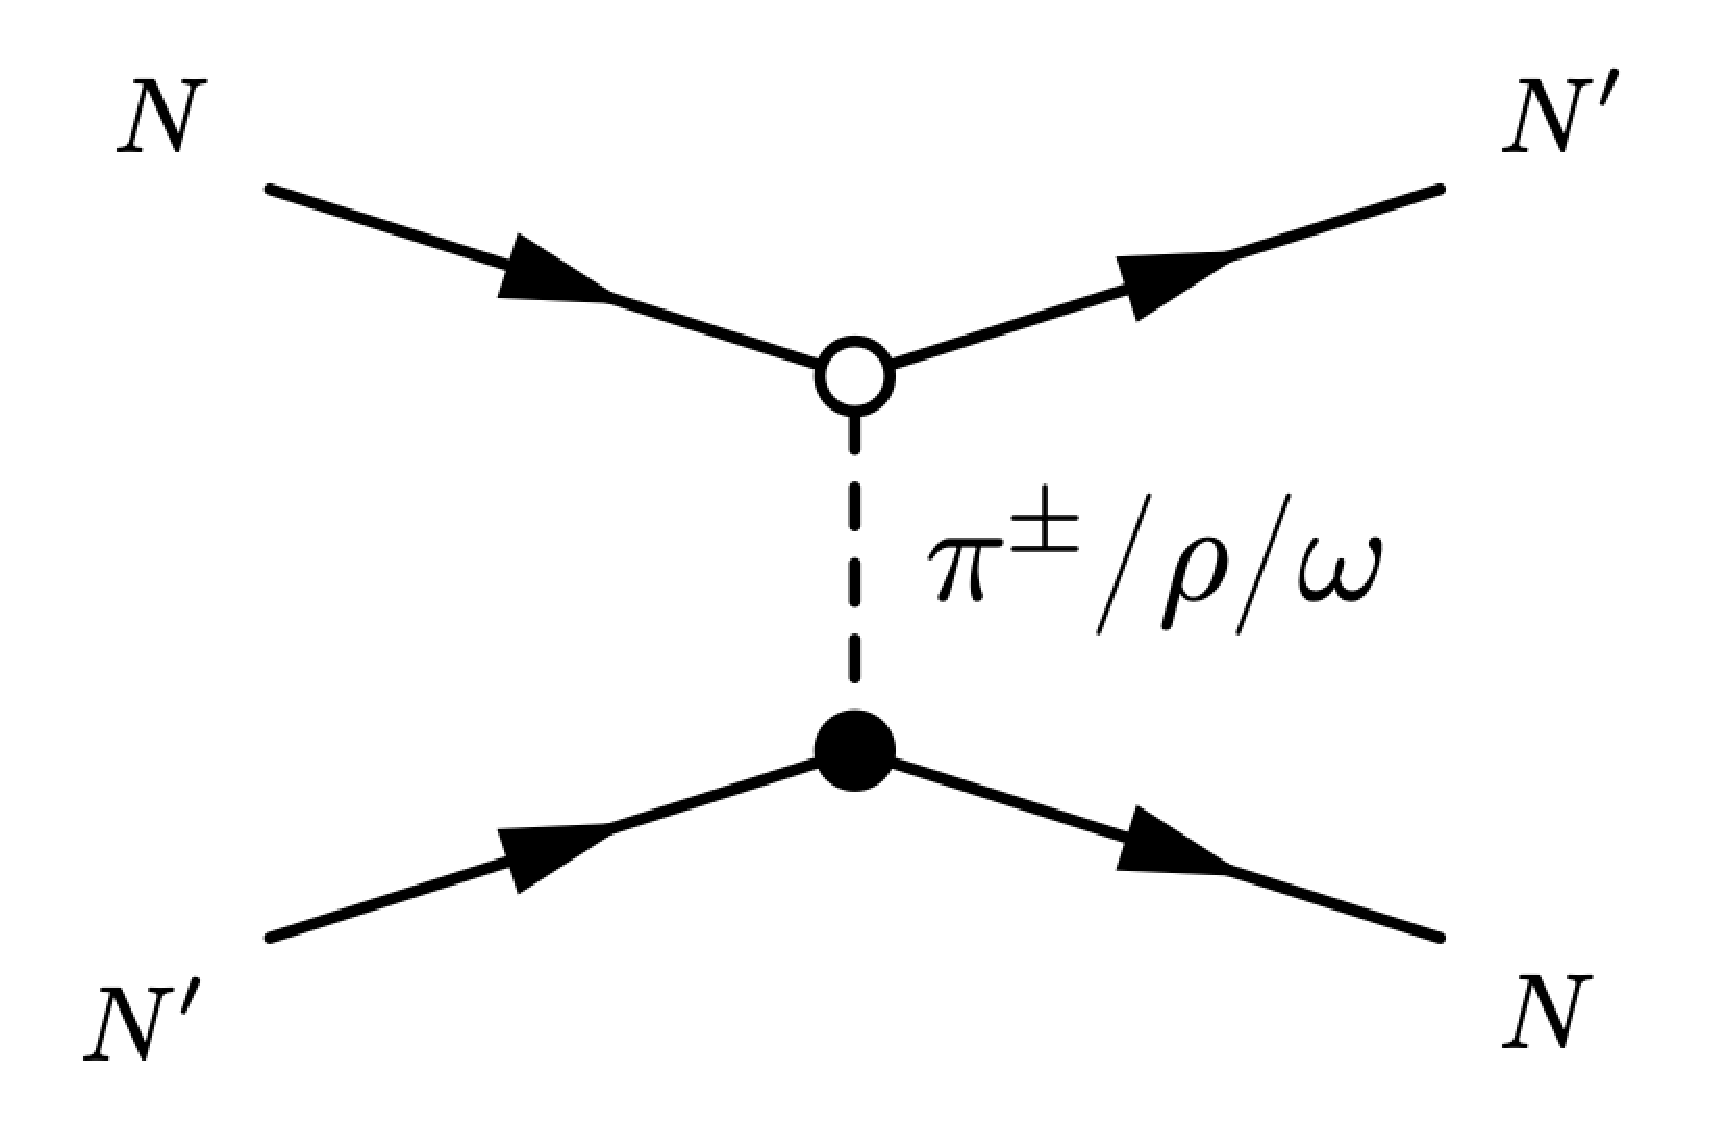
\includegraphics[width=0.3\textwidth]{Fig7_a.eps}

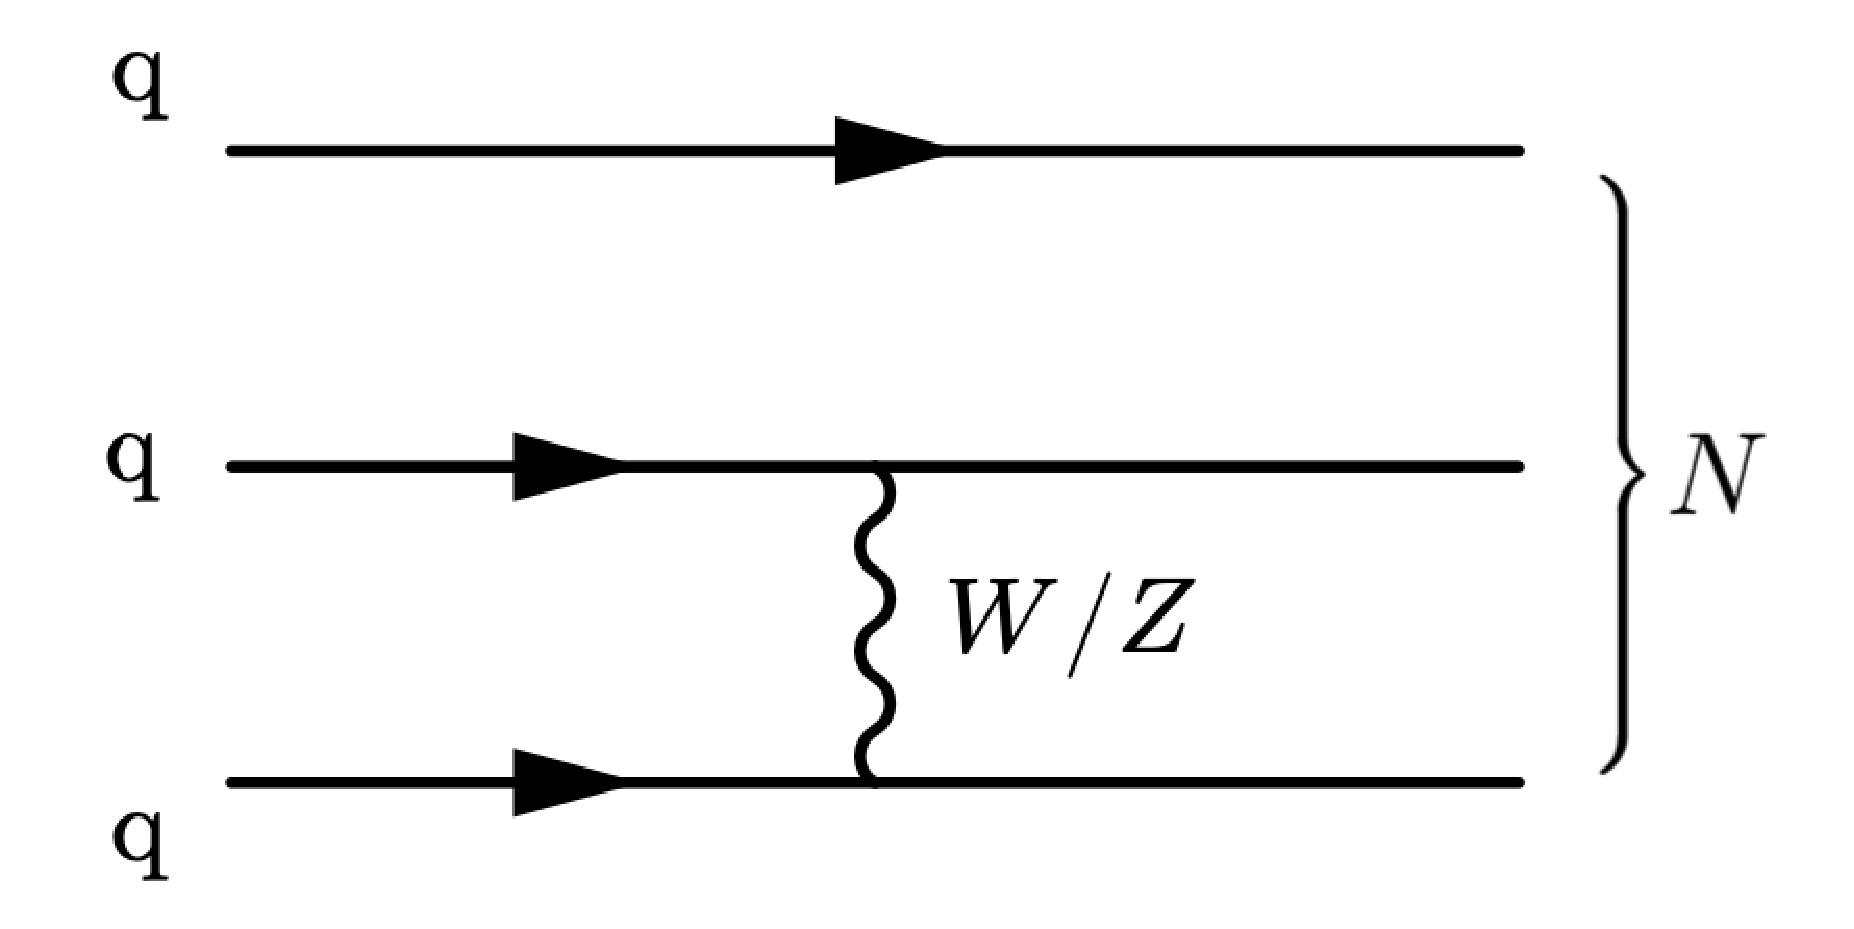
\includegraphics[width=0.3\textwidth]{Fig7_b.eps}
\caption{\textbf{Top:} $P$-violating and $T$-conserving interactions between nucleons ($N$) are mediated by the exchange of mesons, such as $\pi^\pm$, $\rho$ and $\omega$ mesons. 
In the diagram, one vertex (denoted by a white circle) is parity violating and is induced by the exchange of $Z$ or $W$ bosons between constituent quarks, while the other vertex (denoted by a black circle) is parity conserving. 
\textbf{Bottom:} Representative quark-level process that induces the parity-violating meson-nucleon vertices via the exchange of a $Z$ or $W$ boson between two quarks within a single nucleon. 
}\label{fig:PVandPC}
\end{figure}
%$\underbrace{\text{----------------------}}_{\rotatebox[origin=c]{-90}{\Large{$N$}}}

%$\underbrace{\text{----------------------}}_{\rotatebox[origin=c]{-90}{\large{N}}}$


\iffalse
\begin{figure}
\centering
\includegraphics[width=0.45\textwidth]{PVandPCvertex.png}
\caption{Weak interactions between nucleons ($N$) are effectively long-range due to the exchange of mesons, \YS{such as $\pi$, $\rho$ and $\omega$ mesons}. 
In the diagram, one vertex is parity violating \YS{and is induced by the exchange of $Z$ or $W$ bosons between constituent quarks}, i.e., involving the exchange of $W$ or $Z$ bosons, while the other vertex is parity conserving. 
\YS{Doesn't $\pi^0$-meson exchange also contribute (besides $\pi^\pm$ exchange)? Maybe we could update the symbol in the diagram to the more general $\pi$?}
\YS{It may be useful also to add a sub-diagram (or a second diagram) showing some representative quark-level processes that induce the PV meson-nucleon vertices; e.g., exchange of a $Z$ or $W$ boson between two quarks within a single nucleon.} 
}
\end{figure}
\fi

%\LC{Victor: \citet{sushkov_nonconservation_1978} 
%Parity nonconservation in heavy atoms due to weak electron-electron interaction. O.P. Sushkov, V.V. Flambaum. Yad. Fiz. 27, 1307, 1978. 
%DB: There are also later works like that of A-Gongora and P. Sandars \citet{gongora_parity_1986}. We should search for papers that refer to this early paper pointed by Victor \citet{ginges_violations_2004, murray_dyons_1999,commins_parity_1980, gongora_spherical_1987} [where \citet{ginges_violations_2004,gongora_spherical_1987} get most citation]. We should also have a look at the refs in this paper itself for even earlier work like that of the \citet{bouchiat_i_1974}. 
%\LCa{07/Jan/2024 : Dima and I stop editing this subsection here and will continue to modify it later.}
%\VF{ Ref. \citet{sushkov_nonconservation_1978} is definitely the first work about effect of e-e PV interaction in atoms. It was motivated by the absence of PV in atoms declared by wrong measurements by Fortson and Sandars groups in 1976, concluding that Weinberg model is wrong, so we searched for new contributions. I do not think that any other reference is needed since e-e contribution is about 4Z times smaller than e-N  PV and any further corrections are much smaller than experimental and theoretical accuracy. In the Standard model there is further suppression by factor $4 \sin^2 \theta_W -1=-0.07$.  
%\LC{DB: We need to remember that parity violation was also observed in e-e scattering \citet{slac_e158_collaboration_observation_2004}. I believe, there was a later high-precision measurement \citet{moller_collaboration_moller_2014}. We should mention this.}
%\subsection{Atomic parity violation -Misha, Victor} \label{Sec:Impact_AtomicPV}

%The topic of atomic parity violation (APV) was partly addressed in the Introduction, Sec.\ \ref{Sec:Intro-motiv-APV}. 
 
\subsubsection{Molecular parity violation} \label{METH2.PV.MPV}

Prediction of the parity-violating weak neutral currents within the electroweak theory led to the emergence of a whole new field of atomic physics. However, the first dedicated experiment to search for the parity non-conservation in atomic-molecular physics was performed much earlier: \citet{bradley_absence_1962} found that mixing of levels of opposite parity in the  O$_2$ molecule  was less than $3 \times 10^{-8}$ [see also a review of early PV calculations and measurements by \citet{fortson_atomic_1984}]. 

Molecules, particularly diatomic ones like BaF and RaF radicals,
%, or TlF molecule, 
are considered promising systems for studying PNC effects 
%\MK{I suggest to cite here an old, but still useful review 
\cite{sushkov_parity_1978-1,kozlov_topical_1995}.
%}. \LC{Thanks, Misha.}
These molecules have closely spaced energy levels of opposite parity, which can be mixed by electroweak interactions. Molecular PNC effects have not yet been directly observed, even though various experimental approaches have been proposed, such as Stark interference and optical rotation techniques. 
%\YS{I'm not sure if we explicitly define the acronym ``PNC'' in this review. We should try to do this at the first opportunity and consider adding the acronym to Table\,\ref{Table:abbreviations}.} \LC{done}

A variety of new approaches to molecular parity-violation experiments are being developed \cite{safronova_search_2018}. For example, \citet{demille_using_2008} introduced a Stark interference technique for measuring nuclear spin-dependent parity violation in diatomic molecules, applicable to a broad spectrum of atomic systems.
%\MK{atomic numbers, or atomic systems?}. 
%\YS{Thank you for adding, Lei. This looks good to me.} 
Most recently, \citet{blanchard_using_2023} propose to measure the effect induced by the $P$-violating, $T$-conserving interaction of the nuclear anapole moment with electrons in a new type of experiment aimed at probing the nuclear spin-dependent PNC effect using a non-chiral molecule like TlF. 

%\VF{I replaced Schiff moment by anapole moment according to title of your paper Using parity-nonconserving spin-spin coupling to measure the Tl nuclear anapole moment in a TlF molecular beam John W. Blanchard, Dmitry Budker, David DeMille, Mikhail G. Kozlov, and Leonid V. Skripnikov Phys. Rev. Research 5, 013191, 2023} \LC{Ok}
%\YS{Maybe cite/describe also \citet{demille_using_2008}?}\LC{yes, see above.} %\url{https://journals.aps.org/prl/abstract/10.1103/PhysRevLett.100.023003}?}


%\MK{This subsection (below) is very small. Here we discuss only P-odd interactions which affect the spectra of chiral molecules. Molecular NMR effects are discussed in a separate section below. Thus, it may be more logical to move this text to the subsection \ref{METH2.PV}. It can be added to the paragraph about molecular parity violation, or can form a separate paragraph ``Spectroscopy of the chiral molecules''.}


%\LC{kongaul: Polyatomic is redundant as a chiral molecule requies anyway >=4 atoms}, 
In chiral molecules, one can look for the difference in the transition frequencies of the enantiomers caused by the parity-violating electron-nuclear or electron-electron interactions.\footnote{For systems with well-defined parity, there are no energy shifts that are first order in a parity-violating interaction that mixes opposite-parity states. However, a molecule with a given chirality is in a superposition of opposite-parity states and first-order energy shifts are indeed possible. Observation of parity violation in molecules, chiral or otherwise, remains an unmet challenge to this day, see, for example, \citet{quack_parity_2005,schwerdtfeger_search_2010,safronova_search_2018,berger_parity_2019}.}
In the SM, such effects can be caused by $Z$-boson exchange and are suppressed because of the short range of the weak interaction. 
In the electroweak theory, the couplings of the photon and $Z$ boson are of the same order, but an effective dimensional coupling constant for the $Z$ boson, namely the Fermi constant, accounts for the contact nature of the interaction and is proportional to $1/M_Z^2$ \cite{khriplovich_parity_1991}. 
%\LC{kongaul: This statement is not clear to me. The short range is not the reason for suppression. Weak interactions are suppressed because they are weak, i.e. the Fermi coupling constant is on the order of 1e-14 in atomic units.  The short-range nature of the weak interaction leads to an enhancement in heavy atoms compared to light atoms.}
%\MK{The short range is the reason for most of the suppression. Contact interaction takes place only when electron is inside the nucleus, while Coulomb interaction is always present. In the electroweak theory the couplings of the photon and the Z boson are of the same order. Fermi constant is an effective dimensional coupling ($\sim 1/M_Z^2$), which accounts for the contact nature of the interaction. The PNC part of this interaction is velocity-dependent, which adds another suppression $\sim v/c$ and additional factor Z in the scaling ($v/c\sim\alpha Z$). I think, this is nicely explained in the book by Khriplovich \cite{khriplovich_parity_1991}.}
This suppression rapidly decreases with the nuclear charge $Z$. 
%For example, the spin-independent energy shift scales as $Z^5$ \cite{gajzago_weak_1974,zeldovich_energy_1977}. 
For example, the spin-independent energy shift scales as $Z^5$ \cite{gajzago_weak_1974,zeldovich_energy_1977}, or, more precisely, as $Z_1^3Z_2^2$, where $Z_1$ and $Z_2$ are the nuclear charges of the two heaviest nuclei in the molecule \cite{hegstrom_calculation_1980}. 
%\LC{kongaul: 
Note that this scaling requires two heavy atoms with similar nuclear charge number if main-group compounds are considered [the single-center theorem, see \citet{hegstrom_calculation_1980}]. 
%}
%\MK{This is true. We can rewrite previous sentence: This suppression rapidly decreases with the nuclear charge $Z$. For example, the spin-independent energy shift scales as $Z^5$ \cite{gajzago_weak_1974,zeldovich_energy_1977}, or, more precisely, as $Z_1^3Z_2^2$, where $Z_1$ and $Z_2$ are nuclear charges of the two heaviest nuclei in the molecule \cite{hegstrom_calculation_1980}.}
%\YS{Is there a reference for this?} \MK{Refs: E. Gaizago and G. Marx, Atomki Kozl. Suppl. 16, 177 (1974); B. Y. Zel’dovich, D. B. Saakyan, and I. I. Sobel’man, JETP Lett. 25, 94 (1977).}
%Exotic long-range P-odd interactions will not have such strong suppression and such $Z$-scaling (see also atomic parity violation in Sec.\,\ref{METH2.PV}).
On the other hand, the exotic long-range PNC potential terms $V_{12\pm13}$ decrease with the distance as $1/r$ for sufficiently small boson mediator masses. 
%\YS{Do we mean the potential terms $V_{11}$ and $V_{12,13}$ here instead? ($V_{14}$ normally comes paired with the $V_{15}$ term.)} \LC{Dear Misha, could you take a look of this?} \MK{I picked up potentials with $1/r$ behavior. I think, they can be more important for light molecules.}\LC{Ok. In this case, we should consider the latest theoretical framework, where we study $V_{14q+15}$ and it contains not only $1/r$ but also $1/r^2$ and $1/r^3$. $V_{2}$ and $V_{12\pm13}$ are depend only on $1/r$. }
Their atomic amplitudes do not have such 
%strong suppression \LC{kongaul: Sounds a bit odd because this depends heavily on the interaction strength. I guess that the long range effects are suppressed if heavy-element containing molecules are considered} and such 
strong $Z$-scaling as the respective amplitudes of the conventional contact PNC interaction \cite{dzuba_probing_2017} (see also the discussion of atomic parity violation in Sec.\,\ref{METH2.PV.APV}). 
Similarly, we can expect weaker $Z$-scaling in chiral molecules. 
For example, the interaction of a chiral molecule with a $P$-odd cosmic field, discussed below, has two terms, which scale as $Z^4 \alpha^5$ and $Z^2 \alpha^3$, respectively \cite{gaul_parity-nonconserving_2020}.
%\DB{We need an explicit definition of $c_{1,2}$, p-lease! } 
%\LC{Is it this: The constants $c_{1,2}$ represents the coupling of the electron axial-vector currents to the quark-vector currents and the coupling of the electron-vector currents to quark axial-vector currents, repectively.} 
%\YS{Is there a simple definition of the coefficients $c_1$ and $c_2$ that we could give here?}
In the case of light chiral molecules, the conventional $Z$-boson effects are too small 
%\LC{kongaul: Would be good to give an order of magnitude of the effect sizes and currently achievable resolution.}\LC{we not have}
to be observed in current experiments. 
Therefore, observation of an enantiomeric energy difference in light chiral molecules 
%\LC{kongaul: Are there any bounds on these long-range forces? Could we still see them or are they ruled out in the relevant range?} \DB{This is a great question! Our review is supposed to answer this sort of questions: What kind of limits do already exist for a particular type of interactions. Let us use the opportunity to showcase this using this example!} \LC{I'm not sure if we have constraints from light chiral molecules. So comment out forthis moment.} 
near the present level of sensitivity would be an indication of an exotic long-range force. 

%\LC{Questions: Is this recent RaF experiment \cite{udrescu_precision_2024} helpful to set new constraints? Because \cite{dzuba_probing_2017,isaev_laser-cooled_2010} say we can search new physics with the RaF experiments. How about these two papers \cite{norrgard_nuclear-spin_2019,altuntas_measuring_2018}?}
%\MK{The first two references describe proposals for future experiments. The paper \cite{altuntas_measuring_2018} reports results, which can be used to derive limits on exotic PNC interactions, but this has not been done.}  

%\YS{Likewise, is there a reference for long-range PNC in chiral molecules? I think this is too strong of a statement without a supporting reference. In fact, I think the precise wording of the statement is too strong by itself, since if we take the limit of very small coupling constants, the long-range PNC force can in principle be tuned to give rise to much smaller effects than regular $Z$-boson exchange. Has someone estimated what the enantiomeric energy shift would be due to a long-range PNC force, assuming complementary bounds on $g_V g_A$? Such a reference would be very handy here.}  \MK{I tried to enhance the argument above and added reference to atoms \cite{dzuba_probing_2017} and to molecules \cite{gaul_parity-nonconserving_2020}. For the light chiral molecules the conventional $Z$-boson effects are definitely too small to be observed, so if anything is seen there, it must be something exotic. If we are not sure, we can exclude this part.}
%\YS{Thank you for adding the references, Misha. I made some minor suggestions above, otherwise I'm happy with this part.} 


%\LCa{See if we can cite more reference here. }

%Chiral molecules are sensitive to the P-odd cosmic fields
The energies and transition frequencies of chiral molecules can become time-dependent in the presence of a $P$-odd cosmic field  %\cite{gaul_chiral_2020,gaul_parity-nonconserving_2020,roberts_limiting_2014,roberts_parity_2015}. 
(\citealp{roberts_limiting_2014}, \citeyear{roberts_parity_2015}; \citealp{gaul_chiral_2020}, \citeyear{gaul_parity-nonconserving_2020}).
If such a field oscillates at the frequency $\omega=Mc^2/\hbar$, where $M$ is the mass of the constituent boson of the cosmic field, 
%\YS{What is the parameter $m$ in this case? Is this related to the boson mass $M$ that we discuss elsewhere in this review or is this a different mass-energy scale altogether?}, 
the enantiomeric energy splitting also acquires an oscillating component. 
Such effects have not specifically been sought experimentally. 
Nevertheless, some constraints on such $P$-odd cosmic fields have been derived \cite{gaul_chiral_2020} from the published results of a spectroscopic experiment on the chiral molecule CHBrClF \cite{daussy_limit_1999}. Similar work with atoms \cite{roberts_parity-violating_2014} is discussed in Sec.\,\ref{METH2.PV.APV}.

A theoretical discussion of $P$- and $CP$-violating effects in chiral molecules and projections for future experiment were recently given by \citet{baruch_constraining_2024-1}.   

We conclude that molecular PNC experiments present as yet unexplored opportunities to search for exotic interactions.
%[Daussy et al, Phys. Rev. Lett. 83, 1554 (1999)]. 
%\DB{Yes, we should also cross referred to
%\cite{roberts_limiting_2014,roberts_parity_2015}}\MK{done.}

%\LC{Consider cite this one: \citet{baruch_constraining_2024-1}.}
%\LC{YS: In the case of short individual sections, I like the idea of merging the section on molecular spectroscopy with atomic spectroscopy.  One possible approach could be to merge the current section IV B 4 on molecular spectroscopy with section IV B 2 on atomic hyperfine structure.  We could in principle also include or link to discussion of non-hyperfine atomic spectroscopy methods that probe spin-independent forces.} 

%%%%%%%%%%%%%%%%%%%%%%%%%%%%%%%%%%%%%%%%%%%%%%%%%%%%%%
                      % Me2.EDM
%%%%%%%%%%%%%%%%%%%%%%%%%%%%%%%%%%%%%%%%%%%%%%%%%%%%%%
\subsection{EDM experiments }\label{METH2.EDM}

%\LCa{Dear Zhenia, could we move this section to Sec.\,\ref{METH2.EDM}. Dima's opinion now is to merge it with the EDM content there. }.
%\YS{This sounds good to me.  I've moved the text and have merged/rearranged/updated accordingly.}


In the classical picture, an EDM $\boldsymbol{d}$ is a measure of the separation of positive and negative electric charges in a system. \citet{purcell_possibility_1950} proposed the idea that elementary particles, such as electrons, might possess a permanent EDM in addition to their magnetic dipole moment. 
%\DB{Shall we mention that they proposed as a test of P and did not initially realize that there is also T violation by the EDMs? If we do, we need to ``fact-check'' in the original paper!} \LC{[I found \citet{purcell_possibility_1950} wrote "nucleon with an electric dipole moment would show an asymmetry between left-and-right handed coordinate systems", but I didn't notice any words related to time reversal symmetry. So Dima may be correct.] How about we add an sentence like:\
They suggested searching for EDM of elementary particles as a test of $P$ violation. 
Later, it was realized that EDMs also imply time-reversal invariance violation \cite{landau_conservation_1957}. 
%\YS{Could we please add the following reference here: L.D. Landau, Conservation Laws in Weak Interactions, JETP, Vol. 5, No. 2, p. 336 (August 1957) (Russian original - ZhETF, Vol. 32, No. 2, p. 405, August 1957). }
Thus, the existence of an EDM of an elementary particle violates both the $P$ and $T$ symmetries. 
A variety of $P,T$-violating processes within and beyond the SM can generate EDMs of elementary and composite particles, including leptons, nucleons, nuclei, atoms and molecules \cite{ginges_violations_2004,pospelov_electric_2005,engel_electric_2013}. 
Within the SM, EDMs of elementary particles are produced by high-order radiative corrections and are extremely small compared to foreseeable experimental sensitivities. 
Therefore, EDM measurements at present provide a clean probe of ``new physics''. 

% Some old test from the introduction section on EDMs: 
%In the (naive) classical picture, an electric dipole moment (EDM) $\boldsymbol{d}$ arises from the separation of electric charge within a system of nonzero size. 
%Since the underlying electromagnetic forces respect both the parity ($P$) and time-reversal ($T$) symmetries, a classical EDM respects both the $P$ and $T$ symmetries. 
%There it is possible for an EDM to arise for point-like particles (such as the electron). 
%EDMs change sign under the $P$ symmetry operation but not the $T$ symmetry operation, whereas angular momenta do not change sign under the $P$ symmetry operation but do change sign under the $T$ symmetry operation. 
%Hence an EDM of a quantum nature manifestly breaks both $P$ and $T$ invariance. 
%The violation of the $P$ and $T$ symmetries by a quantum EDM is a consequence of underlying interactions that violate the $P$ and $T$ symmetries. 
%\YS{cite the papers [Ginges and Flambaum, Phys.~Rept.~\textbf{397}, 63 (2004)], [Pospelov and Ritz, Annals Phys.~\textbf{318}, 119 (2005)] and [Engel, Ramsey-Musolf and van Kolck, Prog.~Part.~Nucl.~Phys.~\textbf{71}, 21 (2013)] here.} 

%In the quantum realm, however, the situation is different. 
Since an EDM is a vector quantity, it must be directed along the total angular momentum of a system, in accordance with the Wigner-Eckart theorem. 
The EDM of a composite system (nucleon, nucleus, atom) may be due to the $P,T$-violating forces between the constituent particles, which must be spin-dependent. 
Such an interaction is proportional to $\v{s} \cdot \v{v}$, where $\v {s}$ is the spin of the particle and $\v {v}$ is a polar vector. 
In the case of a short-range $P,T$-violating interaction (mediated by a heavy boson), the vector $\v{v}$ may be directed along the gradient of the nuclear or electron density, see, for example, \citet{ginges_violations_2004}. 
A similar interaction between nucleons produces a nuclear EDM.
 However, the electron shielding effect needs to be taken into consideration \cite{schiff_measurability_1963}. It turns out that the electric field of a nuclear EDM is completely screened by atomic electrons outside the nucleus. Inside a nucleus of finite size, this field survives and is known as the Schiff-moment field \cite{flambaum_nuclear_2002}.
%According to the Schiff theorem, the electric field of a nuclear EDM in atoms is completely screened outside the nucleus \cite{schiff_measurability_1963}. Inside a nucleus of finite size, this field survives and is known as the Schiff-moment field \cite{flambaum_nuclear_2002}. \DB{I think this text is extremely confusing for several reasons. What do you think of the following:  However, various shielding effects need to be taken into consideration \cite{schiff_measurability_1963}. It turns out that the electric field of a nuclear EDM is completely screened outside the nucleus. Inside a nucleus of finite size, this field survives and is known as the Schiff-moment field \cite{flambaum_nuclear_2002}.  }
This field polarizes the atom and creates an atomic EDM. 
Such EDMs have been experimentally constrained for Hg \cite{graner_reduced_2016}, Xe (\citealp{rosenberry_atomic_2001}; \citealp{allmendinger_measurement_2019}; \citealp{sachdeva_new_2019}),
%\cite{allmendinger_measurement_2019,rosenberry_atomic_2001,sachdeva_new_2019},
%\YS{please also add the following Xe experimental paper reference: https://journals.aps.org/prl/abstract/10.1103/PhysRevLett.123.143003}
Ra \cite{bishof_improved_2016} and Yb \cite{zheng_measurement_2022} atoms and the TlF molecule (\citealp{hinds_electric_1980}; \citealp{cho_search_1991}; \citealp{dzuba_electric_2002}).
%\cite{dzuba_electric_2002,hinds_electric_1980,cho_search_1991}. 
%\MK{I think, the last EDM experiment with TlF was reported in \cite{cho_search_1991}.}\LC{Ok}
These experiments give us information about $P,T$-odd interactions in the hadronic sector including limits on the QCD vacuum angle parameter $\theta$, the proton and neutron EDMs, quark EDMs, and quark chromo-EDMs (the quark chromo-EDM interacts with the gluon fields inside a nucleon, while the ordinary EDM interacts with the electric field). 
%\DB{Need tp explain what ``chromo-EDM'' is} 
They also give us limits on the electron-nucleus $P,T$-odd interactions proportional to nuclear spin. 

Such an interaction between electrons and the nucleus proportional to the electron spin \cite{stadnik_improved_2018} or nuclear spin \cite{dzuba_new_2018} may be produced by axion exchange. 
Therefore, measurements of atomic EDMs provide us with information about axions (see Sec.\,\ref{subsec_g_Pg_S}). 

An atomic EDM $d_A$ may also be produced by the interaction of an electron EDM $d_e$ with the atomic electric field. 
This atomic EDM increases rapidly with nuclear charge $Z$, at a rate faster than $Z^3$ (\citealp{sandars_enhancement_1966}; \citealp{flambaum_enhancement_1976}).
%\cite{sandars_enhancement_1966,flambaum_enhancement_1976}. 
The electron EDM enhancement factor $K=d_A/d_e$ in atoms with a valence electron with angular momentum $J$ may be estimated as  \cite{flambaum_enhancement_1976,ginges_violations_2004}:
\begin{equation} 
\label{da}
|K|=|d_A/d_e| \sim \frac{10 Z^3 \alpha^2 R(Z \alpha)}{J(J+1/2)(J+1)^2}\,,
\end{equation}
%\LCa{Dima ask to check this 3 here.}\VF{In fact, factor 3 is a fit of results of the  numerical calculations. There is an analytical estimate in  \cite{flambaum_enhancement_1976} which contains E1 amplitudes, energy denominators and effective principal quantum numbers. This will take a half of page to explain, so I prefer to keep this factor of 3 with reference to \cite{flambaum_enhancement_1976}.}
%\YS{I think the RHS of Eq.~(\ref{da}) is missing a factor of $d_e$. From memory, the numerical pre-factor in the RHS of Eq.~(\ref{da}) depends on the value of $J$ for the atomic state, with smaller values for high-$J$ states, while the relativistic factor $R$ is defined so that $R \to 1$ in the nonrelativistic limit $Z\alpha \to 0$. Would it be worth presenting a simple equation along the lines of Eq.~(143) in \cite{ginges_violations_2004}?} 
where the relativistic factor $R(Z \alpha)$ increases with the nuclear charge $Z$ and tends to unity as $Z\alpha \to 0$, with $\alpha$ being the electromagnetic fine-structure constant. 
%[Sandars,Electron electric dipole moment enhancement in heavy atoms. V.V.Flambaum. Yad. Fiz. 24, 383, 1976 [Sov. J. Nucl. Phys. 24, 199 (1976)]. 
As a result, the atomic EDM of a heavy atom may exceed the bare electron EDM by up to three orders of magnitude; e.g., in Cs, $K \approx +130$; in Tl, $K \approx -500$; in Fr, $K \approx +1000$. 
Note that for an $s_{1/2}$ electron, $K>0$, while for a $p_{1/2}$ electron, $K<0$, since electron spin in $p_{1/2}$ state is directed opposite to the total electron angular momentum $J$.  
%For electrons with higher angular momentum  $J$ the enhancement factor  $K$ decreases as $1/[J(J+1/2)(J+1)^2]$. 

In molecules, this enhancement can be several orders of magnitude larger due to mixing of closely spaced rotational levels of opposite parity by the interaction of $d_e$ with the intrinsic molecular electric field \cite{sushkov_parity_1978-1}.  %and strong electric field inside polar molecules \cite{sushkov_parity_1978-1}. 
Note, however, that this picture of an enhanced molecular EDM in a rotational molecular state corresponds to the limit of a weak external electric field. 
In actual experiments, the electric field $\v{E}$ is sufficiently strong to polarize the molecule along the electric field, since the interaction $\v{D} \cdot \v{E}$ of the intrinsic dipole moment $\v{D}$ of a polar molecule with the external electric field $\v{E}$ is comparable to or even exceeds the small interval between opposite-parity rotational molecular levels. 
In this case, the electron EDM $d_e$ interacts with the so-called intrinsic effective field of a polar molecule, $\v{\epsilon}$, which is directed along the external electric field $\v{E}$ but may exceed it in size by several orders of magnitude [a similar molecular enhancement has been explored in measurements of the proton EDM in TlF molecular experiments, see, for example, \citet{hinds_electric_1980}].\footnote{Note that the effective field $\epsilon$ should not be confused with the real intrinsic electric field inside a polar molecule. For example, the effective field $\epsilon$ and atomic EDM $d_A$ vanish in the nonrelativistic limit and the electron EDM becomes unobservable, in accordance with the Schiff theorem  \cite{schiff_measurability_1963}.}
% [JILA] \LC{do we need to cite the new paper of HfF$^+$ \cite{roussy_improved_2023}}.
%aron_order_2014,meyer_prospects_2008
%\LC{Need Victor to check the reference here.}

Indeed, $\epsilon$ may reach  $\sim 10^{11}$\,V/cm in heavy polar molecules such as ThO \cite{skripnikov_communication_2013,fleig_electron_2014,skripnikov_combined_2016}, 
%\YS{Where does the value of $\sim 10^{12}$\,V/cm for ThO come from? I recall a smaller value of $\sim 10^{11}$\,V/cm for ThO - see, e.g., the papers in \cite{skripnikov_communication_2013,fleig_electron_2014,skripnikov_combined_2016} }\LC{Then perhaps we should change to $\sim 10^{11}$?}%https://pubs.aip.org/aip/jcp/article/139/22/221103/193341/Communication-Theoretical-study-of-ThO-for-the , https://www.sciencedirect.com/science/article/pii/S0022285214000782 , https://pubs.aip.org/aip/jcp/article/145/21/214301/196113/Combined-4-component-and-relativistic}
since $\epsilon$ is proportional to $d_A$ in Eq.\,(\ref{da}) and rapidly increases with $Z$. 
The energy shift is $\delta= -d_e \epsilon \sim d_A  D/R^3$, where $R$ is the distance between the atoms in a molecule.
%and \LCa{$D$ is the dipole moment of the molecule}.
%\DB{This is formally correct but the enhancement saturates at low external field. I think this should be somehow mentioned. I think the best way to do this is NOT not talk about the enhancement factor in molecules but rather about the effective fields. For example: Molecules have closely lying levels of opposite parity and correspondingly large polarizabilities. This means that the molecules can be fully polarized in laboratory experiments leading to enhanced effective internal electric fields as high as $\sim 10^{12}$\,V/cm}. 
% [Sandars,Effects of parity nonconservation in diatomic molecules. O.P. Sushkov, V.V.Flambaum. JETP 48, 608, 1978 (ZhETF 75, 1208, 1978).]. 
As a result, the most stringent limits on the electron EDM and short-range electron-spin-dependent $P,T$-violating interactions between electrons and nucleons were obtained in experiments with molecular ThO \cite{acme_collaboration_improved_2018} and HfF$^+$ \cite{roussy_improved_2023}.
% \YS{It looks like ``ACME'' somehow got lost from the collaboration name. Regarding one of Dima's earlier comments, could we try to remove the ``et al.'' after the collaboration name?} \LC{yes, we will do that soon.} and HfF$^+$ \cite{roussy_improved_2023}. 


%\LC{Check to be consistent with Sec.\,\ref{METH.PM.EDM}.}
% \VF{I suggest to delete text below} --------------------------------------------------------------------------------------------------------
% \DK{I agree with Yevgeny. The charge separation picture is rather a cartoon picture that is, perhaps, not so appropriate at this level for the review. Look, perhaps, at the phrasing of the introductory paragraphs of these references (which should also be included here, I think):\cite{commins_electric_2007,commins_electric_2007-1} 
% %Eugene D. Commins, J. David Jackson, and David P. DeMille, ``The electric dipole moment of the electron: An intuitive explanation for the evasion of Schiff’s theorem.'' American Journal of Physics \textbf{75}, 532 (2007) and the very beautifully written Eugene D. Commins, ``Electric dipole moments of elementary particles, nuclei, atoms, and molecules.'' Journal of the Physical Society of Japan \textbf{76}, 111010 (2007).
% }
% \VF{This discussion is not appropriate in this review. Why we do not discuss what is spin of point-like particle which is a more fundamental problem? Also, discussion below about Zeeman effect and Stern-Gerlach experiment is not needed, everybody knows this. Interaction (d E) does not need an explanation. Sometimes this review goes to elementary school level. This is a waste  of time for a professional physicist reader and will certainly have a negative impact.}


% \YS{This paragraph reads a bit awkwardly to me. The Stern-Gerlach effect involves the MDM, which we say at the end of the paragraph, but maybe it would be better to say this earlier; e.g., that EDMs can be related to spin-dependent interactions in several ways, including in some ways similar to MDMs?}
% \DK{I would cut the paragraph below and replace it with a more relevant paragraph on how electric dipole moments can lead to spin precession in an electric field just as magnetic moments lead to spin precession in a magnetic field. This is how EDMs are searched for practically, so it is makes more sense to present in this way. See discussion in the Commins references above.}
% Electric dipole moments can be related to spin-dependent interactions in several ways. One example is the Stern-Gerlach experiment, which demonstrated the influence of the spin of an electron on its behavior in an external magnetic field. In this experiment, a beam of silver atoms was passed through a region of inhomogeneous magnetic field, and the atoms were deflected in different directions depending on their spin. This experiment demonstrated that the spin of an electron has a magnetic moment, which can interact with an external magnetic field through the spin-dependent interaction known as the Zeeman effect.

% \DB{The reader will have the following questions that we definitely need to address here. 1. Is the EDM interaction a fifth force? I think the answer is yes! 2. If yes, where is it in the catalogs of exotic potentials? I think this is probably monopole-dipole coupling with the monopole being electric charge instead of mass, is this correct? Note that this interaction can be shielded by shielding the electric field. Please comment!}

% \DK{Answering Dima's questions: (1) Mostly ``yes' I think. While I believe that perhaps in principle the EDM could be an intrinsic property of an elementary particle that interacts through the known electromagnetic force, mostly people think about that EDM being induced by a new interaction via coupling to a heavy particle, just as Dima says... it would arise from a loop correction in the interaction between the particle and the photon field. (2) For sure you can have an EDM induced in a composite system by an interaction between constituent particles by exactly the mechanism Dima is proposing: in fact, I think Yevgeny has a paper on this! Turns out we had a similar discussion while writing the review with Marianna! The EDM part of that review \citet{safronova_search_2018} discusses all this in detail to some extent.}


%\LC{One can take reference to Derek PRA 2023 \cite{jackson_kimball_probing_2023}. The paper have a section about "Searches for parity- and time-reversal-violating electric dipole moments (EDMs)"}
%\DK{FYI, this review has now been published and can be referenced: \cite{jackson_kimball_probing_2023}. Also I would suggest looking at and referencing \cite{chupp_electric_2019}.}

%\YS{I've drafted the text below.} \LC{Thanks. Here is a recent review paper of experimental and theoretical efforts to measure the electric dipole moments (EDMs) of fundamental particles \citet{alarcon_electric_2022}, one of the key insights is the importance of EDM measurements in probing physics beyond the Standard Model. We may refer to this paper too.}


%One of the characteristic features of a $P,T$-violating EDM is that the interaction of the EDM with an electric field $\boldsymbol{E}$ produces an energy shift that is linear in the electric field, $\delta \varepsilon = - \boldsymbol{d} \, \cdot \, \boldsymbol{E}$, regardless of the strength of the applied electric field. 
%For example, polar molecules appear to possess large EDMs due to their high polarisabilities that allow near-complete mixing of closely-spaced molecular levels of opposite parity in applied electric fields of modest strength. 
%However, these are not true quantum EDMs, since the energy shifts nevertheless scale quadratically with $\boldsymbol{E}$ at very small electric field strengths. 

The basic idea behind the exploration of the $P,T$-violating EDMs of atoms or molecules is to search for a shift in the energy of an atomic or molecular state that scales as an odd power of the applied electric field; linearly in the low-field limit.
%i.e., $\delta \varepsilon = - \boldsymbol{d} \, \cdot \, \boldsymbol{E}$.\footnote{In contrast, the electric-field dependence of $P,T$-conserving energy shifts of atoms may be approximated by the two-level formula  $(\boldsymbol{E}^2 + E_0^2)^{1/2}$, where $E_0$ is a parameter proportional to the interval between opposite-parity levels. 
%This shift scales quadratically with $\boldsymbol{E}$ for weak electric fields, namely as $\sim \boldsymbol{E}^2/(2E_0)$, and only transitions to a linear scaling with the absolute value $|\boldsymbol{E}|$ for strong electric fields. 
This is in contrast with the $P,T$-even energy shifts, which do not change sign upon reversal of the electric field  $\boldsymbol{E}$. 
% This is different from $P,T$-violating energy shifts, which do reverse sign upon reversal of $\v{E}$.} 

%\MK{We explained earlier that this scaling does not work for molecules. I think this must be rewritten more accurately. The main difference between $P,T$-odd and $P,T$-even effects is that the former change sign with the field reversal, while the latter do not. For the weak field that leads to the linear and quadratic scaling respectively. For the stronger fields this transforms to the dependence on the odd and even powers of the field.}
%scale quadratically with $\boldsymbol{E}$ for weak electric fields and only transition to a linear scaling with $\boldsymbol{E}$  for strong electric fields 
%; i.e., $\delta \varepsilon = - \boldsymbol{d} \, \cdot \, \boldsymbol{E}$.
If one simultaneously applies both electric and magnetic fields in the experiment, in the weak-field limit, the energy shift experienced by the state of interest takes the form $\delta \varepsilon = - \boldsymbol{d} \cdot \boldsymbol{E} - \boldsymbol{\mu} \cdot \boldsymbol{B}$, where $\boldsymbol{\mu}$ is the magnetic moment of the state and $\boldsymbol{B}$ is the magnetic field experienced by the state. 
By first applying the electric and magnetic fields parallel to one another and then reversing the relative direction of the fields, one can elucidate the size of the EDM or place a constraint on it. 
The observed effect in this case manifestly breaks $P$ and $T$ invariance, since the correlation $\boldsymbol{E} \cdot \boldsymbol{B}$ is a $P,T$-odd quantity. 
This traditional approach has been adopted in numerous EDM experiments, including experiments using ultracold neutrons \cite{baker_improved_2006,abel_measurement_2020}, 
%\YS{[Baker \textit{et al}., PRL \textbf{97}, 131801 (2006)], [Abel \textit{et al}., PRL \textbf{124}, 081803 (2020)]}, 
as well as atomic xenon \cite{allmendinger_measurement_2019,sachdeva_new_2019}, 
%\YS{[Allmendinger \textit{et al}., \textbf{100}, 022505 (2019)], [Sachdeva \textit{et al}., PRL \textbf{123}, 143003 (2019)]}, 
mercury \cite{graner_reduced_2016} 
%\YS{[Graner \textit{et al}., PRL \textbf{116}, 161601 (2016); PRL \textbf{119}, 119901 (2017)]} 
and thallium \cite{regan_new_2002}. 
%\YS{[Regan \textit{et al}., PRL \textbf{88}, 071805 (2002)]}. 
A more recent approach employing parity-doublet molecular states that function as an internal comagnetometer has been utilised in experiments using %\YS{
PbO \cite{eckel_search_2013},
%\url{https://journals.aps.org/pra/abstract/10.1103/PhysRevA.87.052130},} 
ThO \cite{acme_collaboration_order_2014,acme_collaboration_improved_2018} and HfF$^+$ \cite{roussy_improved_2023}. 
%\YS{[ACME Collaboration, Science \textbf{343}, 269 (2013)], [ACME Collaboration, Nature \textbf{562}, 355 (2018)]}. 
%\YS{Please note that \cite{acme_collaboration_improved_2018} and \cite{andreev_improved_2018,acme_collaboration_improved_2018} are the same paper, except one uses the first author and the other uses the collaboration name. Could we please use one or the other exclusively in this section and elsewhere in the review?} \LCa{done}.
The advantage of this alternative approach is that the direction of the internal electric field experienced by the molecular electrons can be reversed without necessarily reversing the direction of the applied electric field, eliminating a major source of systematic uncertainty. 
%\LC{consider add this paper \citet{roussy_improved_2023} here?}
%\YS{This sounds good. Done.}

\citet{alarcon_electric_2022} provide a recent overview of experimental efforts to measure the EDMs of fundamental particles, along with a discussion of the importance of EDM measurements in probing physics beyond the SM. 
%Earlier reviews provide detailed discussion of various aspects of EDMs: 
%\citet{ginges_violations_2004} discuss aspects of atomic theory, \citet{pospelov_electric_2005} discuss the generation of EDMs at the nucleon level, while \citet{engel_electric_2013} discuss aspects of nuclear theory. 

To conclude this section, we discuss a point emphasized by \citet{chupp_electric_2015} [see also \citet{fleig_model-independent_2018} and \citet{degenkolb_global_2024}]: it is possible in principle that more than one source of ``new physics'' contributes to an atomic or molecular EDM. 
For instance, in some models, an intrinsic electron EDM appears together with $P,T$-odd electron-nucleon forces, both of which contribute to the EDM of an atom or a molecule. 
To account for such a possibility, one needs to construct two- or higher-dimensional parameter-exclusion regions, which generally enlarges the allowed ranges for individual parameters. 
A combination of different experiments with different relative sensitivities to individual EDM sources can be used to disentangle the individual contributions. 
While such analyses will become essentially important once an EDM is discovered, it is our opinion that the minimalistic approach where limits on individual new-physics sources are derived on the assumption of a unique source are, in most cases, adequate until the time when new physics is discovered. 
We believe, this approach should be favored due to its simplicity and a straightforward way to compare the relative sensitivity of different experiments. %\DB{Dear Theorists: kindly read this carefully and tell us if you agree! I am arguing here with the position of Chupp and Ramsey-Musolf}
%\YS{I agree with the minimalistic approach, generally speaking, being warranted until new physics is discovered. Regarding multi-parameter analyses of EDM experiments, we may consider also mentioning the paper \cite{fleig_model-independent_2018}. %\url{https://link.springer.com/article/10.1007/JHEP07(2018)012}. 
%I think Victor may have also had a similar paper, though I don't recall the reference.} \MK{I agree.}\VF{
The minimalistic approach is additionally justified since, within the same model, different mechanisms often give contributions of different order of magnitude. The electron-nucleus $T,P$-violating interaction (a tree-level effect) normally dominates over the electron EDM (loop level).

\subsection{T-odd, P-even (TOPE) interactions}
\label{METH2.TOPE}

While TOPE interactions had been studied in nuclear physics [see, for example, \citet{uzikov_null-test_2015}; \citet{nikolaev_new_2020} and references therein], \citet{kozlov_possibility_1989} proposed to search for TOPE effects in atomic physics by observing the correlation $\v{k}\cdot\v{E}$ between the wavevector $\v{k}$ of light propagating through an atomic medium subject to a static electric field $\v{E}$.

However, the initial excitement about this proposal was somewhat quenched when \citet{conti_new_1992} pointed out that, under some theoretical assumptions\footnote{In the paper by \citet{conti_new_1992}, EDMs arise from diagrams containing fermionic loops. 
In such loops, one needs to sum over all fermions including quarks and leptons. 
%Thus, the limit from the eEDM can be placed only on some combination of the coupling constants of all fundamental fermions. 
%\YS{
Thus, bounds from the electron EDM can be used to constrain the electron-quark interaction parameter.
%}
%Another constraint follows from the neutron EDM. 
%\YS{
On the other hand, bounds from the neutron EDM can be used to constrain quark-electron and quark-quark interaction parameters.
%}
The diagrams generating an EDM include the exchange of the usual $Z$ boson and a new axial boson. 
The interaction range is determined by the mass of the $Z$ boson, provided that the new boson is lighter than the $Z$ boson; in this case, there is no additional suppression of the TOPE effect from the mass of the second boson. 
The mass of the new boson becomes important only if it is larger than the mass of the $Z$ boson.}, stringent limits could be put on TOPE effects from the limits on ($P$- and $T$-odd) EDMs, since TOPE interactions are generated from EDMs via radiative corrections involving the ``usual'' $P$-violation in weak interactions. 

Nevertheless, experiments were carried out with atomic thallium \cite{hopkinson_interferometric_2002}, but found no evidence of the TOPE effect. 

One may ask if it is possible to study TOPE interactions using the exotic spin-dependent potentials as discussed in this review?  Examination of the symmetries of the potentials reveals that the only TOPE interactions are those described by $\sV_{6,7}$, see Eq.\,\eqref{DM_eqV67}. 

Exotic potential terms of the $\sV_{6,7}$ type, which are $T$-odd, $P$-even, may arise from a combination of Eq.\,(\ref{Lagrangian_vector}) and an analog of Eq.\,(\ref{Lagrangian_tensor}): 
\begin{equation} 
 \label{TOPE}
 \begin{aligned}
\mathcal{L}_{Z'} = Z'_{\mu} \sum_\psi \bar{\psi}\gamma^{\mu}\left(g_V^\psi + \gamma_{5}  g_A^\psi  \right) \psi \\
+ Z'_{\mu \nu} \sum_\psi \bar{\psi}\sigma^{\mu \nu} ( g_{T} + i g_{\tilde{T}} \gamma_5) \psi  \, . 
 \end{aligned}
\end{equation}
% where $Z'_{\mu\nu}$ is defined similar as $P_{\mu\nu}$ in Eq.\,\ref{Lagrangian_tensor}, i.e. $Z'_{\mu\nu} = \partial_{\mu} Z'_{\nu} - \partial_{\nu} Z'_{\mu}$ is the field-strength tensor of the field $Z'_{\mu}$. \DB{Discussion of the term with mass here. Does it vanish or not?}
%\YS{In Eq.\,\eqref{TOPE} and in the sentence here, may I suggest to use the notation $g_T$ and $g_{\tilde{T}}$ instead of $g_t$ and $g_{pt}$ for consistency with our use of the symbols for tensor and pseudotensor elsewhere in our review?} 
%\LC{Yes, thanks!}
% \DB{We need to refine this statement:}
Finally, we remark that the Lagrangian used by \citet{porsev_quadrupole_1994} contains a cross term proportional to $g_A g_{\tilde{T}}$ in the interaction between two fermions according to our Eq.\,\eqref{TOPE}. 

Experimental searches for $\sV_{6,7}$ were reported by \citet{hunter_using_2014} (see the description of their work employing the Earth spins as a source in Sec.\,\ref{g_Vg_A_e-n}), by  
\citet{ji_new_2018} with a shielded spin source and a SERF magnetometer as discussed in Sec.\,\ref{Sec:EXP.METH.1}, by \citet{xiao_exotic_2024} using a novel alkali-magnetometer technique, and by \citet{huang_new_2024} using two NV-center ensembles. 

There were also suggestions to search for TOPE interactions by analyzing energy level statistics in nuclei and atoms with dense spectra \cite{french_symmetries_1987,morrison_proposed_2012}. A recent proposal suggests using atomic polarizabilities as a probe for testing TOPE \cite{lahs_polarizabilities_2024}.


% One can also find other research about T-odd, P-even in %\citet{kozlov_possibility_1989}; \citet{khriplovich_what_1991}; \citet{conti_new_1992}; \citet{porsev_quadrupole_1994}; 
% \citet{nikolaev_new_2020}. 

 




%%%%
\subsection{Particle \texorpdfstring{$g$}{g}-factors}
\label{METH2.g-factor}

%\YS{15/12/2023: Started new section on $g$-factor measurements.} 
%\YS{16/12/2023: First draft ready.} 

The $g$-factor of a particle relates its magnetic dipole moment $\v{\mu}$ to its angular momentum $\v{J}$ according to: 
\begin{equation}
    \label{g-factor_definition}
    \v{\mu} = g \frac{e}{2m} \v{J} \, , 
\end{equation}
%where the plus sign is for positively charged particles \DB{or neutral particles, e.g., the neutron,} and the minus sign is for negatively charged particles, \DB{Dear Zhenia, dear All, We do not know how to resolve this without having this ugly $\pm$ or ending up with $g=-2$ for the electron. What we have now is our best attempts. Do you have better ideas? For neutrinos, it is ugly $b/c$ it is not clear what to put as the reference mass. Do people even talk about neutrino g-factors?}
%\DB{Zhenya, do you agree with this? The definition as given before was problematic for electrons and negative muons...}
%\YS{Dear Dima, in the earlier version of this equation, I treated $g$ as a signed quantity (I understand that $g$ sometimes is defined as the absolute value or magnitude of the $g$-factor though). I think the addition of the $\pm$ sign and explanation after the equation is confusing, since, e.g., neutrons and antineutrons have nonzero $g$-factors, but are electrically neutral particles. The sign of $g$ has nothing to do with the overall electric charge of a particle, but it is true that the sign of $g$ reverses when going from a particle to its antiparticle or vice versa.} 
where $e$ is the elementary electric charge (equal to the magnitude of the charge of the electron) and $m$ is the particle or reference mass. 
%\LC{YS: 
The $g$-factor can be either positive or negative depending on the (anti)particle species; e.g., $g_e \approx -2$ for the electron, while $g_{e^+} \approx +2$ for the positron. 
Note that in atomic physics, the electron spin $g$-factor $g_s$ is often defined as the absolute value of $g_e$; i.e., $g_s = |g_e| = -g_e$. 
%}
It is common to parameterize the magnetic moment of the electron in terms of the Bohr magneton $\mu_\textrm{B} = e \hbar / (2 m_e)$ and to parameterize the magnetic moments of nucleons in terms of the nuclear magneton $\mu_\textrm{N} = e \hbar / (2 m_p)$.

% In the case of a classically rotating \DB{Zhenia, let us discuss. Rotating bodies is such a can or worms... Do you want to talk moments of inertia, etc. here?} 
% \YS{Good point. Maybe we could instead say ``
In the case of a body of mass $m$ and electric charge $q = e$ orbiting on a classical trajectory, %...''?} 
% or orbiting body of mass $m$ and electric charge $q = e$, 
the $g$-factor associated with the orbital motion of the body is $g = 1$. 
This $g$-factor value remains unchanged in the quantum theory of elementary spin-$1/2$ particles, including leptons and quarks, with respect to their orbital angular momentum. 
In the case of the intrinsic spin angular momentum of an elementary spin-$1/2$ particle, however, the $g$-factor value is $g = 2$ in the Dirac theory. 

Small deviations from the Dirac value of $g = 2$ arise due to quantum radiative (loop) corrections, parameterized by the anomalous magnetic moment $a = (g-2)/2$. 
The leading one-loop correction to the electron $g$-factor in QED was computed by Schwinger and found to be $a = \alpha / (2\pi)$ \cite{schwinger_quantum-electrodynamics_1948}. 
%\YS{Cite: https://doi.org/10.1103/PhysRev.73.416}. 
Corrections to the $g$-factor of the electron have been computed to the five-loop level in QED, as well as to lower orders in weak and hadronic processes \cite{aoyama_theory_2019}, 
%\YS{Cite:  https://doi.org/10.3390/atoms7010028} 
and provide the basis for a stringent test of the SM via comparison with experiment \cite{fan_measurement_2023}. 
%\YS{Cite: https://doi.org/10.1103/PhysRevLett.130.071801}. 
In the case of the muon, there is presently some disagreement between experiment and theoretical predictions for the $g$-factor of the muon, potentially hinting at possible new physics beyond the SM \cite{keshavarzi_muon_2022}.
%\YS{Cite: https://doi.org/10.1016/j.nuclphysb.2022.115675}. 

The existence of new bosons with couplings to the SM according to Eqs.\,\eqref{Lagrangian_scalar} -- \eqref{Lagrangian_tensor} would modify the $g$-factors of fermions via quantum loop-level processes involving these virtual bosons (see Fig.\,\ref{yan2019-fig} for an example of a one-loop-level process). 
These loop processes are distinct from the %classical 
%\DB{What does ``classical'' mean here? Do we need this word?} \YS{``Classical'' here implies that the processes contribute in the limit $\hbar \to 0$ (as opposed to ``quantum'' processes, which don't survive in the same limit). The single-boson-exchange-induced processes that are the focus of our current review are tree-level processes and are manifestly classical processes. In principle, the terms ``classical'' and ``tree-level'' are synonymous in this context, so we could remove the word ``classical'' here without loss of meaning.} 
tree-level forces that are the focus of the present review. 
By studying these loop-level processes, one can place constraints on interactions of exotic bosons. 
The $g$-factors of leptons (such as the electron and muon) provide sensitivity to much feebler couplings of new bosons than the $g$-factors of nucleons and nuclei, principally due to the elementary (i.e., non-composite)  
%\DB{I do not get the meaning of ``elementary'' here} \YS{What we mean here is ``elementary particle'' or ``fundamental particle''; i.e., a particle that, as far as we can tell, is not composed of other more basic particles.} 
and non-hadronic nature of the former, which results in cleaner and more precise standard-model predictions. 
For discussions and calculations of the contributions of new bosons to lepton $g$-factors, see, e.g., \citet{karshenboim_constraints_2014}; \citet{chen_muon_2017}; \citet{yan_constraining_2019}; \citet{davoudiasl_muon_2023}; \citet{agrawal_searching_2023}; \citet{ema_muon_2024}.
%\YS{Cite: https://doi.org/10.1103/PhysRevD.90.073004, https://doi.org/10.1103/PhysRevD.95.115005, https://doi.org/10.1140/epjc/s10052-019-7442-8}. 

The $g$-factor of a particle can be experimentally determined from measurements of the Larmor spin-precession frequency $\nu_\textrm{s}$ and cyclotron frequency $\nu_\textrm{c}$ of the particle, according to the relation: 
\begin{equation}
    \label{g-factor_measurement}
    \frac{g}{2} = \frac{\nu_\textrm{s}}{\nu_\textrm{c}} \, . 
\end{equation}
In the case of stable particles, measurements of $g$-factors can be performed using cold particles in Penning traps. 
Penning-trap experiments have been used to measure the $g$-factors of the electron (\citealp{hanneke_new_2008}; \citealp{fan_measurement_2023}),
%\cite{hanneke_new_2008,fan_measurement_2023},
%\YS{Cite: https://doi.org/10.1103/PhysRevLett.100.120801, https://journals.aps.org/prl/abstract/10.1103/PhysRevLett.130.071801}, 
proton \cite{schneider_double-trap_2017}
%\YS{Cite: https://www.science.org/doi/10.1126/science.aan0207} ,
and antiproton \cite{smorra_parts-per-billion_2017}. 
%\YS{Cite: https://doi.org/10.1038/nature24048}. 
In the case of antiprotons, measurements should be performed in ultra-high-vacuum conditions in order to minimise the probability of antiproton-proton annihilation via collision of the antiproton with residual gas in the experimental chamber. 
In the case of intrinsically unstable particles with short lifetimes, measurements of $g$-factors can be performed using relativistic particles in storage rings in order to increase their lifetime in the laboratory frame of reference. 
Storage-ring experiments have been used to measure the $g$-factors of the muon and antimuon \cite{muon_g-2_collaboration_final_2006,muon_g-2_collaboration_measurement_2021,muon_g2_collaboration_measurement_2023}. 
%\YS{Following one of Dima's earlier suggestions, could we try to remove the ``et al.'' after the collaboration name?} \LC{Done}
%\cite{muon_g-2_collaboration_final_2006,muon_g2_collaboration_measurement_2021,muon_g2_collaboration_measurement_2023}.
%\YS{Cite: https://doi.org/10.1103/PhysRevD.73.072003, https://doi.org/10.1103/PhysRevD.103.072002, https://doi.org/10.1103/PhysRevLett.131.161802}. 



%Discuss which momentum scales contribute/dominate to/in the g-factor contributions of new bosons in virtual loop processes? 


%\LCa{Can we put the figure and content below in this section?}
%\YS{Thank you for adding the figure, Lei. I like the figure and I've merged your suggested text into one of the paragraphs above. Please check.} 
%\LC{Thanks you so much!}
%If the exotic particle exists, its exchange between the lepton and the antilepton would generate the anomalous lepton moments. Fig.\,\ref{yan2019-fig} shows a Feynman diagram for this process. From the constraints on these moments one can thus obtain constraints on the exotic particles and their interactions.


\iffalse
\begin{figure} [!htbp]
\begin{center}
\includegraphics[width=0.3\textwidth]{Yan2019.png}
\end{center}
\caption{Modification of a lepton's electromagnetic vertex by exchange of a `new' boson (dashed line), 
%\YS{
which can give rise to contributions to the magnetic and/or electric dipole moment(s) of the particle.
%} 
The wavy line represents a photon and the solid lines represent the lepton. 
The labels indicate the four-momenta of the particles. 
Figure from \citet{yan_constraining_2019}. %\MK{It seems to me, that something is wrong with momenta: pluses should be changed to minuses.}
} \label{yan2019-fig}
\end{figure}
\fi

\iffalse
% This code is good for produece the final fenyman diagram
\begin{figure}
%\centering
\begin{fmffile}{Yan}
  \begin{fmfgraph*}(100,80) % Width and height of the diagram
    % Define the vertices
    \fmftop{i1} % Photon at the top
    \fmfbottom{o1,o2} % Fermions at the bottom
    % Incoming and outgoing fermions

    \fmf{fermion,tension=1,label=\large{$p$}}{o1,v1}
    \fmf{fermion,tension=1,label=\large{$p-k$},label.side=left}{v1,v2}
    \fmf{fermion,tension=1,label=\large{$p'-k$},label.side=left}{v2,v3}
    \fmf{fermion,tension=1,label=\large{$p'$},label.side=right,label.side=left}{v3,o2}
    % Dashed line interaction
    \fmf{dashes,right=0.3,tension=0.0,label=\large{$k$}}{v1,v3}
    % Photon interaction
    \fmf{photon,label=\large{$q$}}{v2,i1}
  \end{fmfgraph*}
\end{fmffile}
%\vspace{3mm}
\caption{Modification of a lepton's electromagnetic vertex by exchange of a `new' boson (dashed line), which can give rise to contributions to the magnetic and/or electric dipole moment(s) of the particle.
The wavy line represents a photon and the solid lines represent the lepton. 
The labels indicate the four-momenta of the particles. 
Figure modified from \citet{yan_constraining_2019}.
}
\label{yan2019-fig}
\end{figure}
\fi


\begin{figure}
\centering
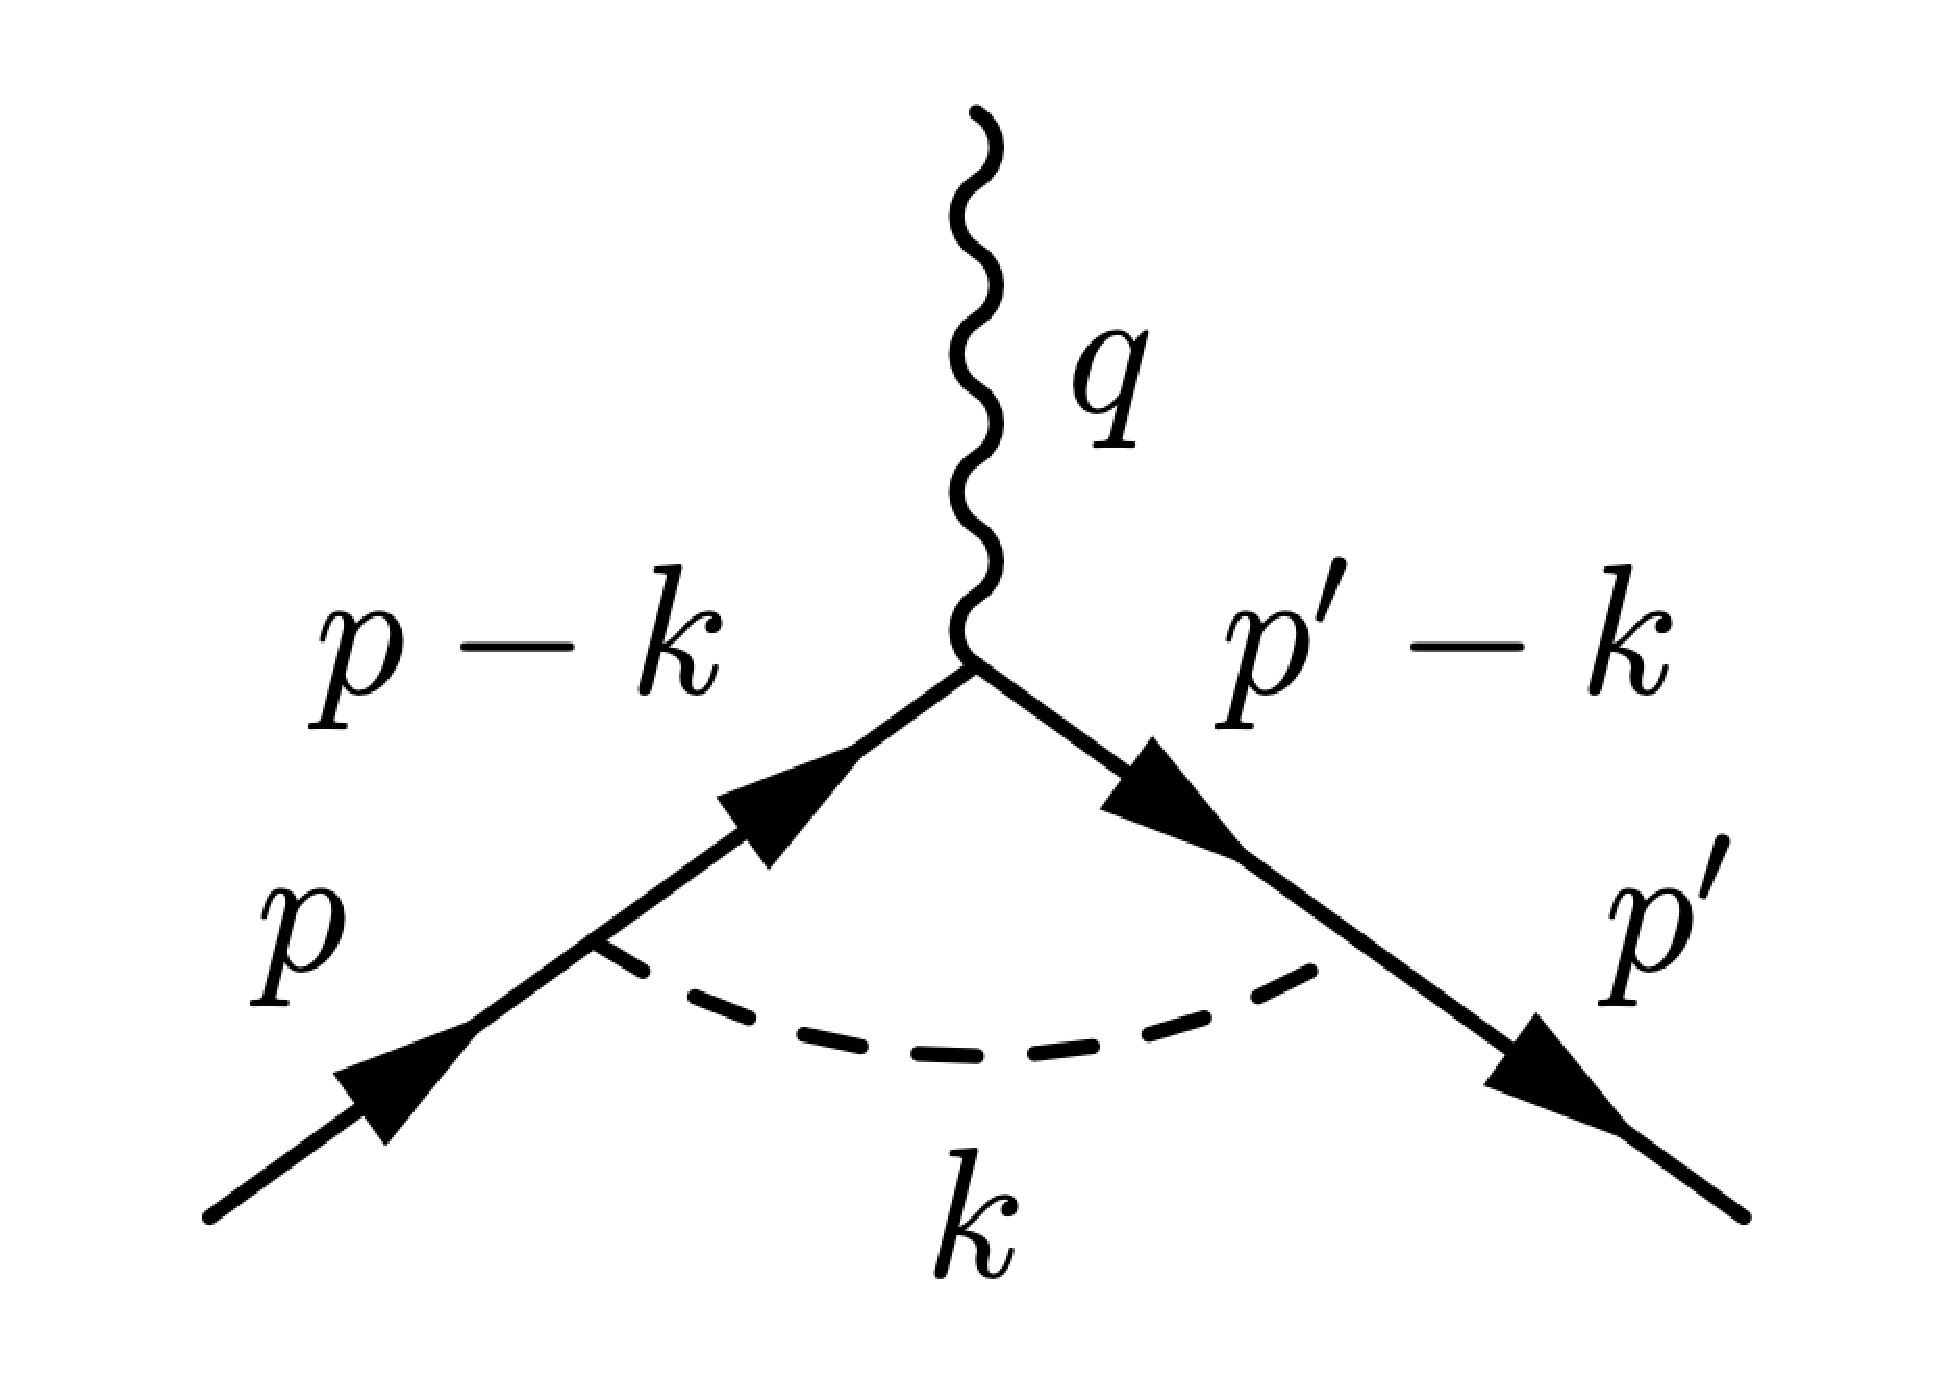
\includegraphics[width=0.27\textwidth]{Fig8.eps}
%\vspace{3mm}
\caption{Modification of a lepton's electromagnetic vertex by exchange of a `new' boson (dashed line), which can give rise to contributions to the magnetic and/or electric dipole moment(s) of the particle.
The wavy line represents a photon and the solid lines represent the lepton. 
The labels indicate the four-momenta of the particles. 
Figure modified from \citet{yan_constraining_2019}.
}
\label{yan2019-fig}
\end{figure}

%\DB{It would be nice to say something here along the lines of: we present the constraints on exotic particles extracted from the $g-2$ experiments as given by the original authors in Sec. ....}
%\YS{I agree. I think Lei knows the relevant references and the places to link to.} \LC{Yes, do you think the gray line in Fig. 4 of \citet{delaunay_probing_2017} and blue line in Fig. 2 of \citet{frugiuele_current_2019} is constraints from $g-2$ experiments. If so, we have presented them in Fig.\,\ref{V1-fig} in App.\,\ref{appendix_V1}. You mentioned "According to Ref.~[20]\cite{andreas_constraints_2010} of \citet{bollig_muons_2020}, the muon $g$-factor constraint is (in translated form) given by $g_p^\mu \lesssim 8 \times 10^{-4}$ for masses $\lesssim m_\mu$." }
%\YS{Dear Lei, Yes, these references discussed bounds from $g$-factor measurements and comparison to theory. Another relevant reference is \cite{yan_constraining_2019}.} 


%In Fig.\,\ref{V1-fig}, we present the constraints on exotic interactions extracted from the $g-2$ experiment-to-theory comparison, as obtained by \citet{delaunay_probing_2017} and \citet{frugiuele_current_2019}.

In Fig.\,\ref{gpgs-fig}, we present the constraints on exotic interactions extracted from the $g_e - 2$ experiment-to-theory comparison, as reported by \citet{agrawal_searching_2023}. 
Similarly, in Fig.\,\ref{V1-fig}, we present the constraints from \citet{delaunay_probing_2017} and \citet{frugiuele_current_2019}.



%%%%%%%%%%%%%%%%%%%%%%%%%%%%%%%%%%%%%%%%%%%%%%%%%%%%%%
                      % Me2.IS
%%%%%%%%%%%%%%%%%%%%%%%%%%%%%%%%%%%%%%%%%%%%%%%%%%%%%%
\subsection{Isotope shifts    }\label{METH2.IS}
%\label{Sec:Intro-motiv-Isotope}

New interactions conserving $P$ and $T$ symmetries can be searched for using the spectra of simple atomic systems (hydrogen, antiprotonic helium, muonium, positronium), where the accuracy of both theory and experiment is high, and so any unaccounted contribution would be noticeable, see Sec.\,\ref{METH2.PM.AHS}, \ref{METH2.PM.EA}, \ref{Sec:limits_main} and \citet{potvliege_deuterium_2023}. 

In heavy atoms, the best theoretical accuracy is about 0.1\% (which is much worse than in simple atomic systems), and so the comparison of experiment and theory generally leads to mild limits. 
An exception, however, involves isotope shifts. 
Consider, for example, two atomic transitions. 
If we plot an appropriately normalized frequency of one transition versus another transition, then to a high accuracy, the resulting plot will be a linear function. 
Such a graph is called a King plot \cite{king_isotope_1984}. 
A new interaction mediated, for instance, by a scalar particle can violate the linearity of a King plot. 
Thus, King plots may be used as a tool to search for new Yukawa-type interactions between electrons and the nucleus \cite{berengut_probing_2018}. 
The main challenge from the point of view of theory here is to accurately calculate the small corrections that produce nonlinearities of the King plot within the SM, see, for example, \citet{flambaum_isotope_2018}. 

%[V.V. Flambaum, A. Geddes, A.V. Viatkina, Isotope shift, non-linearity of King plot and search for new particles, arxiv: 1709.00600, Phys. Rev. A 97, 032510 (2018)]. 
%---------------------
%\cite{antypas_isotopic_2019}
%\cite{debierre_tests_2022}
%\cite{berengut_probing_2018}
%\LC{isotope shifts \cite{antypas_isotopic_2019} \cite{debierre_tests_2022}
%\cite{berengut_probing_2018-1}}
%a related reference \cite{debierre_fifth-force_2020}
%\LC{Piet Schmidt, Jose Crespo, Marko; Vladan Viuletic, Tanja   we need to discuss current research situation with a paragraph. The same is for other sections above. \cite{rehbehn_sensitivity_2021}.}

Several recent experiments have searched for King-plot nonlinearities in chains of stable zero-nuclear-spin isotopes; see, for example, \citet{rehbehn_sensitivity_2021}; \citet{figueroa_precision_2022,hur_evidence_2022,ono_observation_2022}; \citet{door_search_2024}. For more details, see a recent review by \citet{kawasaki_nuclear_2024}.

%\DB{Dear Theorists: please check if you agree. This is a retelling of a discussion between Victor and myself.} 
The analyses of King-plot nonlinearities have so far been limited to zero-nuclear-spin isotopes to avoid the complications of including the first- and second-order effects of hfs that would need to be evaluated to high accuracy in order to extract the isotope shifts for nonzero-nuclear-spin isotopes. Recent \cite{berengut_second-order_2024} and ongoing \cite{ginges_notitle_2023} theoretical work considers the possibility of using nuclei with nonzero spin and averaging over the hyperfine structure. 
This raises a question: Could precision isotope-shift comparisons involving nonzero-spin isotopes be useful in searching for exotic spin-dependent interactions? 
Corrections to King plots, after averaging over first-order hyperfine and exotic spin-dependent interactions, contain smaller second-order terms. 
It remains to be seen whether the high accuracy in isotope-shift measurements could eventually compensate for this smallness. 
% \YS{If the effect of the exotic spin-dependent interaction is second order, then my guess is probably not.} \VF{I agree. Nuclear spin  creates problems with accuracy of King plot interpretation  and no obvious enhancement for exotic spin-dependent effects compare to hyperfine interaction which is similar to exotic spin-dependent interaction. This is different for spin-indpendent Yukawa - type interaction which may be  long range while IS field shift is contact. }
 
% Now the main source of information about exotic spin dependent interaction are simple systems like muonium and positronium, where theoretical accuracy is high.
% I do not know how heavy atoms may compete with this. Theoretical uncertainty is 1\% vs $10^{-6}$ in simple systems.

%\LCa{YS: this paper \cite{potvliege_deuterium_2023} is very much relevant to our review in the context of isotope-shift spectroscopy of simple atoms. }


%\YS{Spectroscopy of regular atoms (like hydrogen and helium, as well as King's plot nonlinearity measurements in heavier atoms) can be included.} \LCa{Dima and Misha agreed.} \LCa{There is an Isotop shift section later Sec.\,\ref{METH2.IS} also talked about King's plot, so perhaps not here? We could link to the content talk about hydrogen and helium in the main text.}
%\YS{I agree with the suggestion to describe the relevant techniques in Sec.\,\ref{METH2.IS} with a cross-reference back to the relevant section describing spectroscopy of simple atoms.} 
%\LCa{Hi, Zhenia, do you think we need to change the title of Sec.\,\ref{METH2.PM.AHS} from Atomic hyperfine structure to Atomic spectroscopy to cover more content?}% And how should we link Sec.\,\ref{METH2.IS} with Sec.\,\ref{METH2.PM.AHS} is not so clear to me. }
%\YS{I like the idea of expanding the scope of Sec.\,\ref{METH2.PM.AHS}. Regarding the title, I guess it depends what we plan to have in each section. For example, would Sec.\,\ref{METH2.PM.AHS} focus on spectroscopy of simple atomic systems, while this section focuses on isotope-shift measurements in many-electron atomic systems in the context of King plots? Technically, hydrogen-deuterium comparisons are also a type of isotope-shift spectroscopy.} \LC{I think the first paragraph of Sec.\,\ref{METH2.PM.AHS} is not about hyperfine structure, it is about Atomic spectroscopy. And we didn't have a section to talk about Atomic spectroscopy. So we can modify a little the title to a more generalized one: Atomic spectroscopy.} \YS{I like the updated section title.} \LC{Thanks}

%\LC{Do you mean the J-coupling study of HD in \citet{ledbetter_constraints_2013} when you say hydrogen-deuterium comparisons?}
%\YS{I had in mind something more like in \cite{karshenboim_precision_2010}, but now that I look at the paper again, it looks like he placed limits separately for atomic H and D. I think the paper \citet{ledbetter_constraints_2013} focuses on molecular HD, which is different from the atomic comparisons I had in mind.} \LC{Ok, I see.}



%%%%%%%%%%%%%%%%%%%%%%%%%%%%%%%%%%%%%%%%%%%%%%%%%%%%%%
                      % Me2.DM
%%%%%%%%%%%%%%%%%%%%%%%%%%%%%%%%%%%%%%%%%%%%%%%%%%%%%%
\subsection{Dark matter experiments    }\label{METH2.DM}
%\section{The Limits for New Boson -Derek}\label{sec_newboson}
%%%%% 


Throughout this review we discuss experiments where a local source and a spin-based sensor are used to search for exotic spin-dependent interactions mediated by ``new'' bosons (Sec.\,\ref{Sec:EXP.METH.1}). 
Another possibility is that these new bosons could have been abundantly generated in the early universe and therefore constitute all or part of the dark matter responsible for gravitational effects observed throughout the universe as noted in Sec.\,\ref{Sec:Intro-motiv-DM}. 
In such cases, the presence of these new bosons could be directly detected through their spin-dependent interactions with electrons or nuclei; in other words, no ``source'' (other than the Big Bang that produced the relic background of dark matter) is required for the experiment.\footnote{In contrast to the virtual (off-shell) bosons mediating interactions between a source and a sensor, relic bosons of cosmological origin are ``on-shell.''} 
Detectors designed to measure the interaction of particles comprising the dark matter halo within which the Milky Way galaxy is presumably embedded are known as \emph{haloscopes}. Haloscope experiments using spin-based sensors are reviewed by \citet{graham_experimental_2015,graham_spin_2018}, \citet{safronova_search_2018}, \citet{jackson_kimball_search_2023}, \citet{flambaum_searches_2023}, and \citet{jackson_kimball_probing_2023}.
Here we only briefly outline key features of such searches and their relationship to the source/sensor-type experiments that are the focus of this review. For further information, see the aforementioned reviews and references therein.

At the outset, we emphasize that most reported constraints on exotic bosons and their interactions derived from haloscope experiments are based on the additional assumption that the exotic bosons make up the majority of dark matter.
The key point is that haloscope experiments are actually sensitive to a combination of the interaction strength and (the square root of) the fraction of the dark matter density composed of the bosonic field probed.
Thus reported constraints on the coupling constants from haloscope experiments are weakened if the exotic bosons do not in fact make up a significant fraction of dark matter.
%\YS{I think the assumption that exotic bosons make up the majority of the dark matter is too strong. It's true that the vast majority of experiments present bounds on interaction strength under the assumption that such exotic bosons make up the entirety of the dark matter content. However, we only need to assume that the exotic bosons make up \textit{some} fraction of the dark matter. The experiments themselves are strictly sensitive to a combination of interaction strength and (square root of the) dark matter density. I think we should clarify this point.} 
Interpretation of limits from source/sensor-type experiments (Sec.\,\ref{Sec:EXP.METH.1}) explicitly do \emph{not} require this assumption. 
In this sense, constraints on exotic spin-dependent interactions from source/sensor-type experiments are independent of cosmological models and assumptions and, consequently, more robust. 

A crucial characteristic determining the physical manifestation of bosonic dark matter is the relationship between the boson mass $M$ and the local dark matter density $\rho_\textrm{DM}$. 
At the position of our solar system within the Milky Way galaxy, the estimated average dark matter density is $\rho_\textrm{DM} \approx 0.3-0.6~\textrm{GeV}/c^2$ 
(\citealp{strigari_reconstructing_2009}; \citealp{pato_systematic_2010}; \citealp{catena_novel_2010}; \citealp{salas_dark_2021}),
%\cite{pato_systematic_2010,catena_novel_2010,salas_dark_2021,strigari_reconstructing_2009}, 
corresponding to an average mass density
of about one hydrogen atom per a few cubic centimeters. 
Note that if dark matter is made up mostly or entirely of a species of particle with mass $M \lesssim 10$\,eV/$c^2$, then in order to agree with observations it must be a boson. 
This is because for the inferred $\rho_\textrm{DM}$, the Fermi velocity of particles with $M \lesssim 10$\,eV/$c^2$ exceeds the galactic escape velocity. 
If such new bosons have negligible self-interactions and do not form composite structures, they can be treated as independent particles through which the Earth moves, leading to daily and annual modulations of their flux, as discussed, for example, by \citet{freese_colloquium_2013} and \citet{gramolin_spectral_2022}. 
Importantly, such ultralight bosons will on average have extremely high mode occupation number in the local vicinity of Earth. 
In this case, the phenomenology of ultralight bosonic dark matter (UBDM) is well-described by a field oscillating at approximately the Compton frequency, $\omega_c = Mc^2/\hbar$. 
More massive dark matter candidates [such as weakly interacting massive particles, WIMPs --- see reviews by \citet{aleksandrov_search_2021} and \citet{feng_dark_2010}] behave as incoherent individual particles and experiments commonly employ particle detectors that measure, e.g., energy deposition or ionization signals to find them. 
In contrast, UBDM acts as a coherent entity on the scale of the sensor (and potentially also on the scale of terrestrial networks of sensors). 
Consequently, precision measurement techniques, similar to those used in searches for macroscopic-range exotic interactions discussed in this review, can be employed to search for UBDM. 
For up-to-date constraints on UBDM from a wide variety of experiments from all over the world, see \citet{ohare_cajohareaxionlimits_2020-1}, 
where references describing the experiments and associated limits can also be found. See also the reviews by \citet{sikivie_invisible_2021}, \citet{adams_axion_2022}, and \citet{antypas_new_2022}.

Dark matter composed of axions or ALPs (Secs.\,\ref{Sec:Intro-motiv-spin-0} and \ref{Sec:Intro-motiv-quantum-gravity}), spin-0 particles that can possess scalar and pseudoscalar couplings to fermions \cite{moody_new_1984}, provide an illustrative example of the close connection between searches for exotic spin-dependent interactions and dark matter searches using spin-based sensors as haloscopes.
An axion (or ALP) field $a(\bs{r},t)$ is described, approximately, by
\begin{align}
    a(\bs{r},t) = a_0 \cos\left( \bs{k}\cdot\bs{r} - \omega_c t + \phi_0 \right) \, , 
    \label{eq:axion-field}
\end{align}
where $\bs{k} \approx M \bs{v} /\hbar$ represents the nonrelativistic axion wave vector (with $\bs{v}$ being the velocity of the field relative to the sensor), $\phi_0$ is a random phase offset, and $a_0$ is the average oscillation amplitude of the field. 
The average oscillation amplitude of the field can be estimated by assuming that the average energy of the axion field corresponds to the local dark matter energy density $\rho_\textrm{DM}$ \cite{jackson_kimball_search_2023}:
\begin{align}
    a_0^2 \approx \frac{2\hbar^2}{c^2}\frac{\rho_\textrm{DM}}{M^2} \, . 
    \label{eq:axion-field-amplitude}
\end{align}
The axion field exhibits a finite coherence time due to the random kinetic energy of the constituent axions. 
This leads to a broadening of the line shape to $\delta \omega/\omega \sim v^2/c^2 \sim 10^{-6}$ as discussed, for example, by \citet{krauss_calculations_1985} and \citet{gramolin_spectral_2022}.\footnote{The line is not only broadened, but also develops an asymmetric shape, as discussed, e.g., by \citet{derevianko_detecting_2018} and \citet{gramolin_spectral_2022}.} 
Additionally, there are stochastic fluctuations in the amplitude, phase, and $\bs{k}$ of the axion field, as pointed out by \citet{centers_stochastic_2021};  \citet{masia-roig_intensity_2023} and \citet{flambaum_fluctuations_2023}.
% \VF{Fluctuations of atomic energy levels due to axion and scalar fields,V.V.Flambaum,I.B.Samsonov, Phys. Rev. D 108, 075022 , 2023,  DOI: 10.1103/PhysRevD.108.075022.
% You may add this reference here, if you wish. 
In the latter work, limits on dark matter were obtained from measured variances of energy-shift fluctuations (statistical errors). Axion signal may be separated using measurements of higher moments and correlators of energy-shift fluctuations.

The canonical QCD axion discussed in Sec.\,\ref{Sec:Intro-motiv-spin-0} naturally couples to the gluon field and produces an oscillating EDM along the nuclear spin orientation \cite{graham_new_2013,stadnik_axion-induced_2014}, 
%\DK{Add reference: [P. W. Graham and S. Rajendran, New observables for direct detection of axion dark matter, Phys. Rev. D 88, 035023 (2013)]}, 
leading to an interaction described by the Hamiltonian:
\begin{align}
\mc{H}_\textrm{EDM} =  g_d a(\bs{r},t) {\bs{E}}^\star \cdot \bs{\sigma}_N\,,
\label{eq:oscillating-EDM}
\end{align}
where $g_d$ is an associated coupling parameter\footnote{It should be noted that there can be multiple contributions to the coupling parameter $g_d$, which depend on the theoretical model assumed. \citet{graham_new_2013} and \citet{budker_proposal_2014} discuss contributions from oscillating nucleon EDMs, but there can also be significant contributions to $g_d$ from axion-induced $P,T$-violating intranuclear forces as described by \citet{stadnik_axion-induced_2014} and \citet{stadnik_manifestations_2017-1}. For the canonical QCD axion with the usual axion-gluon coupling, the contributions to $g_d$ from axion-mediated intranuclear interactions are dominant in most nuclei, as they arise at the tree level whereas oscillating nucleon EDMs are induced at the one-loop level.} and ${\bs{E}}^\star$ is the electric field acting on the spin \cite{budker_proposal_2014}. 
%\YS{As written, it's not clear what contributions are contained in the coupling parameter $g_d$. \cite{graham_new_2013} and \cite{budker_proposal_2014} discussed contributions from oscillating nucleon EDMs. However, for the canonical QCD axion with the usual axion-gluon coupling, there are much larger contributions in most nuclei coming from axion-induced $P,T$-violating intranuclear forces, see \cite{stadnik_axion-induced_2014} and \citet{stadnik_manifestations_2017-1}.
%\url{https://link.springer.com/book/10.1007/978-3-319-63417-3}.
%The main point is that oscillating nucleon EDMs are induced at the 1-loop level, whereas the intranuclear forces already arise at tree level (thereby avoiding a sizeable loop suppression factor).} 
%\DB{I see a possible readers' confusion here. The term ``effective field'' is often used to describe, for example, an effective magnetic field due to exotic interaction. Here ``efective'' means something completely different. Not sure how to fix this ``compactly"...}
Axions and ALPs can also couple directly to electron ($e$) or nuclear ($N$) spins $\bs{\sigma}_{e,N}$ through a gradient interaction \cite{graham_new_2013,stadnik_axion-induced_2014},
%\DK{Add reference: [P. W. Graham and S. Rajendran, New observables for direct detection of axion dark matter, Phys. Rev. D 88, 035023 (2013)]}, 
described by the Hamiltonian
\begin{align}
\mc{H}_\textrm{grad} = g_{aNN} \bs{\nabla} a(\bs{r},t) \cdot \bs{\sigma}_{N} + g_{aee} \bs{\nabla} a(\bs{r},t) \cdot \bs{\sigma}_{e}\,,
\label{eq:gradient-interaction}
\end{align}
where $g_{aNN}$ represents the axion-nucleon coupling and $g_{aee}$ represents the axion-electron coupling.
The coupling constants in Eq.\,\eqref{eq:gradient-interaction} are related to the pseudoscalar coupling constants in Eq.\,\eqref{Lagrangian_scalar} according to the relations $g_{aNN} = g_p^N / (2m_N)$ and $g_{aee} = g_p^e / (2m_e)$. 
Here the connection to the topic of this review is evident: the coupling constants $g_{aNN}$ and $g_{aee}$ describing the spin-dependent dark matter interaction are closely related to the pseudoscalar coupling constants constrained by source/sensor experiments described in Secs.\,\ref{subsec_g_Pg_S} and \ref{subsec_g_Pg_P}. See, for example, \citet{jackson_kimball_search_2023} for further discussion of the relationship between these effects. 
%\DK{Maybe good for a theorist to double check this statement and make sure I'm not neglecting a factor of $\pi$ or something! Thanks!}
%\YS{We need a definition of the interaction containing $g_p^{e,N}$ in order to make a definitive statement about the correctness or otherwise of Eq.~(\ref{eq:gradient-interaction}). For consistency with the rest of this review, let's suppose that $g_p^{e,N}$ is defined according to Eq.~(\ref{Lagrangian_scalar}) and keep the convention adopted in Eq.~(\ref{eq:axion-field}) for the axion DM field. In this case, it's clear that Eq.~(\ref{eq:gradient-interaction}) is missing a factor of mass (energy) in the denominator. More precisely, using the non-derivative and derivative forms of the axion-fermion coupling in Eqs.~(1) and (D6) of \cite{fadeev_revisiting_2019}, together with Eqs.~(2), (8) and (10) of \cite{stadnik_axion-induced_2014} and the relation $1/f_a \leftrightarrow g_p^{e,N}/(2m_{e,N})$, I find that Eq.~(\ref{eq:gradient-interaction}) should include a factor of $2m_{e,N}$ in the denominator.} 


An example of a haloscope experiment employing a spin-based sensor is the Cosmic Axion Spin Precession Experiment, CASPEr (\citealp{budker_proposal_2014}; \citealp{aybas_search_2021}).
%\cite{budker_proposal_2014,aybas_search_2021} 
%\DK{Add reference: [D. Aybas et al., Search for Axionlike Dark Matter Using Solid-State Nuclear Magnetic Resonance, Phys. Rev. Lett. 126, 141802 (2021)]}.
The similarity in form between the interaction between spins and an axion dark matter field [Eqs.\,\eqref{eq:oscillating-EDM} and \eqref{eq:gradient-interaction}] and the Zeeman interaction of spins with an oscillating magnetic field suggests the use of magnetic resonance techniques in the search for axion dark matter. 
%\YS{Maybe worth clarifying somewhere that this resonant-type approach is mainly suitable at higher axion masses. For lower axion masses, broadband approaches (some of which are mentioned in the paragraph below) become more suitable.} 
This is the approach taken by the CASPEr experiment, which uses NMR to detect $a(\bs{r},t)$ through its coupling to nuclear spins. Experiments that involve NMR measure the dynamics of nuclear spin in the presence of an applied bias field $\bs{B}_0$, which determines the Larmor frequency $\Omega_L = \gamma_N B_0$ ($\gamma_N$ is the nuclear gyromagnetic ratio). 
The hypothetical presence of the continuous oscillating field $a(\bs{r},t)$ [Eq.\,\eqref{eq:axion-field}] along with the aforementioned spin-dependent interactions make the situation analogous to continuous-wave (CW) NMR \cite{aybas_quantum_2021}. 
%\DK{Add reference: [D. Aybas, H. Bekker, J. Blanchard, D. Budker, G. Centers, N. Figueroa, A. Gramolin, D. F. Jackson Kimball, A. Wickenbrock, and A. Sushkov, Quantum sensitivity limits of nuclear magnetic resonance experiments searching for new fundamental physics, Quantum Sci. Technol. 6, 034007 (2021)]}.
In the experiment of \citet{aybas_search_2021}, 
%\DK{Add reference: [D. Aybas et al., Search for Axionlike Dark Matter Using Solid-State Nuclear Magnetic Resonance, Phys. Rev. Lett. 126, 141802 (2021)]} 
a fraction of the $^{207}$Pb nuclear spins in a ferroelectric\footnote{A ferroelectric crystal is used to provide a relatively large effective electric field ${\bs{E}}^\star$ to enhance the EDM signal.} 
PMN-PT crystal [chemical formula (PbMg$_{1/3}$Nd$_{2/3}$O$_3$)$_{2/3}$-(PbTiO$_3$)$_{1/3}$] are initially oriented along an applied magnetic field $\bs{B}_0$ due to their equilibrium thermal polarization. 
The applied magnetic field $\bs{B}_0$ is scanned, and if there was a detectable interaction between the nuclear spins and the axion dark matter, then when $\Omega_L \approx \omega_c$ a resonance would occur. 
Such an interaction would cause the spins to tip away from the direction of $\bs{B}_0$ and precess at $\Omega_L$, generating a time-dependent magnetization that can be measured using, e.g., induction through a pick-up loop. 
The experiment of \citet{aybas_search_2021}
%\DK{Add reference: [D. Aybas et al., Search for Axionlike Dark Matter Using Solid-State Nuclear Magnetic Resonance, Phys. Rev. Lett. 126, 141802 (2021)]}
found no evidence for dark matter axions with masses $162\,{\textrm{neV}}/c^2 \lesssim M \lesssim 166\,{\textrm{neV}}/c^2$, and set upper limits on the parameters $g_d$ and $g_{p}^{N}$ under the assumption that axions are dark matter with the nominal local density. Since the original CASPEr proposal, there have been several haloscope experiments using NMR and electron spin resonance (ESR) methods for the detection of UBDM fields (\citealp{crescini_operation_2018}; \citealp{quax_collaboration_axion_2020}; \citealp{jiang_floquet_2021}; \citealp{bloch_new_2022}).
%\cite{crescini_operation_2018,quax_collaboration_axion_2020,jiang_floquet_2021,bloch_new_2022}.

These haloscope experiments using NMR and ESR %(\citealp{crescini_operation_2018}; \citealp{quax_collaboration_axion_2020}; \citealp{jiang_floquet_2021}; \citealp{aybas_search_2021}; \citealp{bloch_new_2022}) %\cite{aybas_search_2021,crescini_operation_2018,quax_collaboration_axion_2020,jiang_floquet_2021,bloch_new_2022} 
typically are relatively narrow-band and require scanning the applied magnetic field to search for dark matter bosons of different masses, which correspond to UBDM fields oscillating at different Compton frequencies \cite{zhang_frequency-scanning_2024}.
An alternative approach particularly useful for relatively small Compton frequencies ($\lesssim 1$\,kHz) is to use a broad-band spin-based atomic magnetometer or comagnetometer \cite{terrano_comagnetometer_2021,wei_dark_2023}.
These experiments can simultaneously search for axion dark matter in a broad range of masses (as opposed to resonant-type searches that need to scan over specific and typically limited mass ranges).
There have been several such broadband searches carried out in recent years using a variety of spin-based sensors
%; see, for example, work by 
(\citealp{abel_search_2017}, \citeyear{abel_search_2023}; \citealp{wu_search_2019}; \citealp{terrano_constraints_2019}; \citealp{garcon_constraints_2019}; \citealp{smorra_direct_2019}; \citealp{roussy_experimental_2021}; \citealp{jiang_search_2021}; \citealp{schulthess_new_2022}; \citealp{wei_dark_2023}; \citealp{bloch_constraints_2023}; \citealp{xu_constraining_2023}) %\DKIns{
and there are new proposals to expand the sensitivity of such searches \cite{fierlinger_ramsey_2024}.
%}.
%\citet{wu_search_2019,garcon_constraints_2019,jiang_search_2021,terrano_constraints_2019,abel_search_2017,roussy_experimental_2021,schulthess_new_2022,bloch_constraints_2023,xu_constraining_2023,wei_dark_2023,smorra_direct_2019,abel_search_2023}. Similar effects exist, in principle, for vector dark matter coupled to spins, and can be searched for using analogous experimental methods; see, for example, \citet{chen_dissecting_2022,garcon_constraints_2019}.

%\YS{Following on from my comment in the paragraph above, it would be insightful to distinguish between resonant- and broadband-type experiments here. For example, for continuity, we could first mention the other resonant-type experiments, namely the experiments in \cite{crescini_operation_2018,quax_collaboration_axion_2020,jiang_floquet_2021,bloch_new_2022}, then mention the broadband-type experiments that can simultaneously search for axion dark matter in a broad range of masses (as opposed to resonant-type searches that need to scan over specific and typically limited mass ranges). Besides the examples already listed below, a couple of other broadband axion DM searches have been performed in \citet{smorra_direct_2019,abel_search_2023}.}
%\url{https://www.nature.com/articles/s41586-019-1727-9} and \url{https://scipost.org/10.21468/SciPostPhys.15.2.058}.} 
%Several other haloscope experiments have carried out searches for similar UBDM effects using different spin-based sensors, see, for example, work by %\DK{Add references: 
%\citet{wu_search_2019,garcon_constraints_2019,crescini_operation_2018,quax_collaboration_axion_2020,jiang_search_2021,bloch_new_2022,terrano_constraints_2019,abel_search_2017,roussy_experimental_2021,schulthess_new_2022,bloch_constraints_2023,xu_constraining_2023,wei_dark_2023}. 
%[T. Wu et al., Search for Axionlike Dark Matter with a Liquid-State Nuclear Spin Comagnetometer, Phys. Rev. Lett. 122, 191302 (2019)], 
%[A. Garcon, et al., Constraints on bosonic dark matter from ultralow-field nuclear magnetic resonance, Sci. Adv. 5, eaax4539 (2019)], 
%[N. Crescini et al., Operation of a ferromagnetic axion haloscope at $m_a = 58\mu$eV, Eur. Phys. J. C 78, 703 (2018)], 
%[N. Crescini et al., Axion Search with a Quantum- Limited Ferromagnetic Haloscope, Phys. Rev. Lett. 124, 171801 (2020)],
%[M. Jiang, H. Su, A. Garcon, X. Peng, and D. Budker, Search for axion-like dark matter with spin-based amplifiers, Nat. Phys. 17, 1402 (2021)], 
%[I. M. Bloch, G. Ronen, R. Shaham, O. Katz, T. Volansky, and O. Katz, New constraints on axion-like dark matter using a Floquet quantum detector, Sci. Adv. 8, eabl8919 (2022)],
%[W. A. Terrano, E. G. Adelberger, C. A. Hagedorn, and B. R. Heckel, Constraints on Axionlike Dark Matter with Masses Down to $10^{−23}$eV/$c^2$, Phys. Rev. Lett. 122, 231301 (2019)], 
%[C. Abel et al., Search for Axionlike Dark Matter through Nuclear Spin Precession in Electric and Magnetic Fields, Phys. Rev. X 7, 041034 (2017)], 
%[T. S. Roussy et al., Experimental Constraint on Axionlike Particles over Seven Orders of Magnitude in Mass, Phys. Rev. Lett. 126, 171301 (2021)], 
%[Schulthess, Ivo, et al. New limit on axionlike dark matter using cold neutrons. Physical review letters 129.19 (2022): 191801], [Bloch, Itay M., et al. Constraints on axion-like dark matter from a SERF comagnetometer. Nature Communications 14.1 (2023): 5784]}. 
%\LC{dima suggested added two more: xu_constraining_2023,wei_dark_2023.}
%\DK{Add references: [Chen, Y., Jiang, M., Shu, J., Xue, X., & Zeng, Y. (2022). Dissecting axion and dark photon with a network of vector sensors. Physical Review Research, 4(3), 033080] and [A. Garcon, et al., Constraints on bosonic dark matter from ultralow-field nuclear magnetic resonance, Sci. Adv. 5, eaax4539 (2019)]} .

The haloscope experiments referenced above rely on models that assume the UBDM behaves as a collection of non-interacting bosons described by the standard halo model \cite{evans_refinement_2019}.
%\DK{Add reference: N.W. Evans, C. A. O’Hare, C.McCabe, Phys. Rev. D 99, 023012 (2019).}. 
These models neglect any small-scale structures in the dark matter halo beyond the natural stochastic fluctuations \cite{centers_stochastic_2021}.
%\DK{Add reference: [G. P. Centers, J. W. Blanchard, J. Conrad, N. L. Figueroa, A.Garcon, A. V. Gramolin, D. F. Jackson Kimball, M. Lawson, B. Pelssers, J. A. Smiga et al., Stochastic fluctuations of bosonic dark matter, Nat. Commun. 12, 7321 (2021)]}. 
Consequently, the sensors in these experiments are assumed to be continuously exposed to the UBDM field. 
However, it is possible that the energy density of the UBDM field is concentrated in larger composite structures that form, for example, due to self-interactions among the dark matter bosons (including gravity), or topological effects. 
In such scenarios, Earth would spend most of its time in regions of space with little or no dark matter. 
As a result, Earth would only occasionally and briefly encounter dark matter, resulting in infrequent and short-lived signals in dark matter detectors. 
In theory, a single sensor could detect such transient events. 
However, sensor networks offer more robust detection and verification of potential signals and reduced background of spurious signals. 

The Global Network of Optical Magnetometers for Exotic physics searches (GNOME) was the first such sensor array proposed to target such large composite dark matter structures (\citealp{pospelov_detecting_2013}; \citealp{pustelny_global_2013}; \citealp{afach_characterization_2018}, \citeyear{afach_search_2021}).
%\cite{pospelov_detecting_2013,pustelny_global_2013,afach_characterization_2018,afach_search_2021}.
%\DK{Add references: [M. Pospelov, S. Pustelny, M. P. Ledbetter, D. F. Jackson Kimball, W. Gawlik, and D. Budker, Detecting Domain Walls of Axionlike Models Using Terrestrial Experiments, Phys. Rev. Lett. 110, 021803 (2013)], 
%[Szymon Pustelny, Derek F. Jackson Kimball, Chris Pankow, Micah P. Ledbetter, Przemyslaw Wlodarczyk, Piotr Wcislo, Maxim Pospelov, Joshua R. Smith, Jocelyn Read, Wojciech Gawlik, and Dmitry Budker, The Global Network of Optical Magnetometers for Exotic physics (GNOME): A novel scheme to search for physics beyond the Standard Model, Annalen der Physik 525(8-9), 659–670 (2013)], 
%[S. Afach et al., Characterization of the Global Network of Optical Magnetometers to search for Exotic physics (GNOME), Physics of the Dark Universe 22, 162 (2018)], 
%[S. Afach et al., Search for topological defect dark matter with a global network of optical magnetometers, Nature Physics 17, 1396 (2021)]}. 
The GNOME experiment conducts simultaneous measurements of spin-dependent interactions of composite dark matter objects 
(\citealp{pospelov_detecting_2013}; \citealp{jackson_kimball_searching_2018}; \citealp{grabowska_detecting_2018})
%\cite{pospelov_detecting_2013, jackson_kimball_searching_2018,grabowska_detecting_2018} 
%\DK{Add references: [M. Pospelov, S. Pustelny, M. P. Ledbetter, D. F. Jackson Kimball, W. Gawlik, and D. Budker, Detecting Domain Walls of Axionlike Models Using Terrestrial Experiments, Phys. Rev. Lett. 110, 021803 (2013)], 
%[D. F. Jackson Kimball, D. Budker, J. Eby, M. Pospelov, S. Pustelny, T. Scholtes, Y. V. Stadnik, A. Weis, and A. Wickenbrock, Searching for axion stars and Q-balls with a terrestrial magnetometer network, Phys. Rev. D 97, 043002 (2018)] 
%and
%[Grabowska, Dorota M., Tom Melia, and Surjeet Rajendran. Detecting dark blobs. Physical Review D 98.11 (2018): 115020]}
using atomic magnetometers and comagnetometers in magnetically shielded environments at widely separated locations. The GNOME experiment looks for correlated signals across the network with particular spatio-temporal patterns, associated with different hypothetical exotic-physics scenarios \cite{afach_what_2023},
which help differentiate genuine signals from unrelated background noise. Similar experiments using atomic clock networks have searched for scalar dark matter 
(\citealp{derevianko_hunting_2014}; \citealp{wcislo_experimental_2016}, \citeyear{wcislo_new_2018}; \citealp{roberts_search_2017}, \citeyear{roberts_search_2020}).
%\cite{derevianko_hunting_2014,wcislo_experimental_2016,roberts_search_2017,wcislo_new_2018,roberts_search_2020}. 
There have also been related proposals by \citet{stadnik_enhanced_2016} to carry out a network-based clock-cavity comparison and by \citet{stadnik_searching_2015} and \citet{grote_novel_2019} to use a network of laser interferometers for dark matter searches.
Yet another application of sensor networks for dark matter detection is the idea of \citet{budker_axion_2020} to search for correlated signals from relativistic axions emitted from the decay of axion-quark ``nuggets'' \cite{zhitnitsky_nonbaryonic_2003}.
%\DK{add citation: A.R. Zhitnitsky, J. Cosmol. Astropart. Phys. 10 (2003) 010}.
The use of astrophysical pulsar networks, which have much larger ``apertures'' than terrestrial networks, was discussed by \citet{stadnik_searching_2014}.


%\YS{I don't think any of these searches or the 2014 proposal involved either atom or laser interferometry. These were either clock-based or used clock-cavity nodes. The clock-cavity comparison method was suggested in \citet{stadnik_enhanced_2016}, %\url{https://journals.aps.org/pra/abstract/10.1103/PhysRevA.93.063630}, 
%while laser interferometry was discussed in \citet{stadnik_searching_2015,grote_novel_2019}.
%\url{https://journals.aps.org/prl/abstract/10.1103/PhysRevLett.114.161301} and \url{https://journals.aps.org/prresearch/abstract/10.1103/PhysRevResearch.1.033187}. 
%The use of astrophysical pulsar networks, which have larger ``apertures'' than terrestrial networks, was discussed in \citet{stadnik_searching_2014}.}
%\url{https://journals.aps.org/prl/abstract/10.1103/PhysRevLett.113.151301}.} 
%\DK{Add references: [A. Derevianko, M. Pospelov, Nat. Phys. 10, 933 (2014)], 
%[P. Wcislo, P.Morzynski, M. Bober, A. Cygan, D. Lisak, R. Ciurylo, and M. Zawada, Experimental constraint on dark matter detection with optical atomic clocks, Nat. Astron. 1, 0009 (2016)], 
%[B. M. Roberts, G. Blewitt, C. Dailey, M. Murphy, M. Pospelov, A. Rollings, J. Sherman, W. Williams, and A. Derevianko, Search for domain wall dark matter with atomic clocks on board global positioning system satellites, Nat. Commun. 8, 1195 (2017)], 
%[P. Wcislo et al., New bounds on dark matter coupling from a global network of optical atomic clocks, Sci. Adv. 4, eaau4869 (2018)], 
%[B. M. Roberts et al., Search for transient variations of the fine structure constant and dark matter using fiber linked optical atomic clocks, New J. Phys. 22, 093010 (2020)]}. 

Note also that spin-based sensors can be used in the search for more massive, particle-like dark matter candidates with masses $M\gg 1$\,eV$/c^2$. 
For instance, \citet{fitzpatrick_effective_2013} describes spin-dependent interactions that could be used for the detection of WIMP dark matter. 
%\DK{Insert reference: S. Rajendran, N. Zobrist, A. O. Sushkov, R. Walsworth, and M. Lukin, A method for directional detection of dark matter using spectroscopy of crystal defects, Phys. Rev. D 96, 035009 (2017).} 
\citet{rajendran_method_2017} propose to use nitrogen-vacancy-center spin spectroscopy in diamonds to measure WIMP-induced damage tracks and perform directional detection of WIMPs. 
This would enable searches for WIMPs below the background limits set by the neutrino floor. Another example is the proposal of \citet{lyon_single_2024}
%\DK{insert reference: [Lyon, S. A., et al. "Single phonon detection for dark matter via quantum evaporation and sensing of He 3." Physical Review D 109.2: 023010 (2024)]} 
to use magnetic moment measurements for single-$^3$He-atom detection to find $^3$He atoms evaporated from a van der Waals liquid-helium film by energy transferred in WIMP collisions. 
Related ideas involving spin-dependent interactions of dark matter particles inducing observable collective effects in condensed matter systems are explored by \citet{trickle_effective_2022}. 
Note that \citet{fitzpatrick_effective_2013} and \citet{trickle_effective_2022} categorize boson-mediated spin-dependent interactions of WIMP dark matter in a manner similar to the categorization of boson-mediated spin-dependent potentials between fermions discussed in Sec.\,\ref{Sec:formalism} of this review, illustrating the close connection between the detection of wave-like UBDM and particle-like WIMPs.

%\YS{Suggestion to help better link the discussion of WIMP DM with the core of this review --- It may be worthwhile remarking that \cite{fitzpatrick_effective_2013} and \cite{trickle_effective_2022} provide categorisations of boson-mediated spin-dependent interactions of WIMP dark matter, similar to the categorisations of boson-mediated spin-dependent potentials between fermions discussed in Sec.~\ref{Sec:formalism}.}

In summary, the existence of dark matter is one of the most compelling reasons to search for the existence of exotic bosons, and there are a plethora of experiments testing the UBDM hypothesis, many employing spin-based sensors. There is a strong overlap and cross-fertilization between the underlying theories and the experimental techniques employed in searches for exotic spin-dependent interactions and spin-based dark matter haloscope searches. 

%\LC{\DB{ shall this been mentioned \citet{fierlinger_ramsey_2024} ?}\YS{The paper's not directly relevant to the main topic of boson-mediated spin-dependent forces, but it would fit nicely in Sec. IV G in the context of (planned) dark-matter experiments based on spin-dependent signatures. }}\LC{Perhaps we let Derek decide shall we and where exactly we include this paper.}\DK{I added the reference above in the related section :).}\LC{Thank you!}
%\LC{DB: shall we mention this \cite{ema_probing_2024}?}
%\DK{I propose to make this section rather brief instead of too extensive, as the review is long already and this is an extremely rich area with lots of results. I think maybe just give an overview and highlight a couple experiments to show the connection. These sorts of experiments are extensively reviewed in other papers and books.}

%\LC{DB: yes, agree.}

%\LCa{DK: Dark matter searches only test the scenario where the new boson is a significant or dominant component of dark matter produced by mechanisms in the early universe -- and therefore the new bosons could in principle exist but not be the dark matter, and then be discovered in the long-range spin-dependent force experiments we describe. So, in fact, dark matter constraints do not apply or rule out the tests we describe. However, in the other direction, the long-range spin-dependent force experiments can rule out various dark matter searches since they directly constrain the coupling parameters if the new boson exists. }
%\YS{There's no requirement that a new boson comprise a significant or dominant fraction of the DM to search for such DM-based signatures (though it is preferable). We only require that there be a nonzero local density of DM that is made up of such bosons.} 

%\DB{A reminder: somewhere we need to discuss the relation of exotic potentials to things like nonlinear isotope shifts (-Victor), EDM experiments (-Victor and Yevgeny), $g-2$ (-Yevgeny), parity-violation experiments (-Misha), as well as cosmology and astrophysics (-Yevgeny). What do we mean here? Let us take the example of atomic PV. The isotopic comparison of PV in Yb atoms has led to limits on light $Z^\prime$ bosons. The PV interaction ($\vec{\sigma}\cdot \vec{p}$ is a spin-dependent interaction. But how can we connect this to our 16 potentials? And the same for the other things...}



%\LC{parity-violation, EDM\cite{dzuba_probing_2017,stadnik_improved_2018}}

%\LC{$g-2$:g-2 experiment 41,44,45 [Wei et al., 2022, p. 4]}

%\LC{\citet{vasilakis_limits_2009} may helpful for this section.}

%\LC{PQ-Axion limits and fifth force experiments \citet{arvanitaki_resonantly_2014}}

%\YS{May I ask what the motivation for this section is? 
%We already discuss limits on new bosons in Sec.\,\ref{Sec:limits_main} above. 
%Are there certain aspects that we plan to discuss here which couldn't be discussed there?} 

%\LC{disc. 7}

%-------

%\LCa{Below are some old notes from old Sec. "LIMITS FROM DARK MATTER EXPERIMENTS - DEREK". A mixture of discussions about dark matter and EDM. It would be nice if Zhenia Dima, or Derek could have a look and place them in corresponding section, perhaps Sec.\ref{METH2.DM}.}
%\YS{I've had a look and agree - I've now moved these notes to the dedicated section on dark matter.}

%Dark matter searches are usually interpreted under the assumption that all of dark matter is constituted by particles (fields) of one particular sort, for example, ALPs. Knowing the local dark matter density ($\approx$ 0.4\,GeV/cm$^3$) and assuming the value of ALP mass, one derives their local number density. A further common assumption known and the standard halo model, there is a particular velocity distribution of dark matter from which one can derive the ALP-signal lineshapes \cite{gramolin_spectral_2022}. With these assumptions, one can derive the limits on ALP couplings to fermions. 

%The examples of such limits are shown in Figs.\,\ref{}. \DB{Plots for ALP EDM and gradient couplings; discuss how to relate to the rest of this paper. Emphasize that this is based on a lot of assumptions and that the 5th force searches are more general.}

%\LC{ \citet{ackerman_dark_2009} talks about Dark matter and dark radiation. 
%Another reference may help \cite{sidharth_dark_2021}, it revisit the problems of dark energy and dark matter and several models designed to explain them, leading to the hypothetical fifth force in the light of some latest findings.}

%\LC{The reason people can set limits on the strength of ALP interactions with other types of matter using these assumptions is that by understanding the distribution and number density of ALPs in the universe, one can make predictions about how often ALPs should interact with other types of matter, such as fermions. For example, if one know that there are a certain number of ALPs present in a given area of space, and they know that the ALPs have a certain interaction strength with fermions, they can calculate how often the ALPs should be interacting with fermions in that area of space. By conducting experiments to search for these interactions, one can measure the actual rate of interactions and compare it to the predicted rate. If the measured rate is significantly lower than the predicted rate, it sets a limit on how strong the interaction between ALPs and fermions can be. If the measured rate is in agreement with the predicted rate, it could give evidence that ALPs exist, providing a hint towards solving the mystery of dark matter.}

%\YS{I think it would be nice to include discussion of ultralight dark-matter-induced spin-dependent effects with limits on axion-fermion and axion-gluon/EDM couplings (the axion-gluon coupling is a more fundamental dimension-5 coupling, compared to the dimension-6 axion-EDM coupling, but we can in principle discuss both). 
%Limits come from (co-)magnetometry experiments, NMR-style experiments (including resonant type), spin-polarized torsion pendula experiments, $g$-factor measurements via Penning traps or storage rings, etc. 
%These types of effects are for wavelike dark matter in the sub-eV mass region, but there are also searches for spin-dependent interactions of heavier (fermionic) WIMPs using bulk detectors (including traditional WIMP detectors and possibly also neutrino-type detectors). 
%I'm not sure if we need to discuss the latter types of effects in detail, but it would be good to at least mention this possibility with some references to the relevant literature. 
%--- [UPDATE (24/03/23)]: Wei Ji mentions to include the paper  \cite{trickle_effective_2022}. 
%I can also suggest the paper \cite{fitzpatrick_effective_2013}. 
%There are probably at least several other related papers discussing spin-dependent effects of WIMP-type DM. The main aspects of these papers that are interesting in the context of the present review are that they systematically address the different possible types of spin-dependent interactions that (fermionic) WIMP DM can have with ordinary matter and the implications for experiments that search for WIMP DM.} 

%\YS{If discussing ultralight dark-matter-induced spin-dependent effects, what about also discussing photon-polarization-dependent effects due to the axion-photon coupling? 
%For example, vacuum birefringence, dichroism effects, etc.
%Photon polarization is in some ways analogous to fermion spin.}

%\LC{reference to Sec.\,IX in \citet{safronova_search_2018}: is light dark matter different to ultralight dark matter (\textmu eV)? }
%\YS{I think the use of the terminology ``light'' and ``ultralight'' is somewhat arbitrary. Some people, e.g., use the term ``light'' in the context of DM to mean sub-MeV particles.} 
%\LC{disc. 8}
%%%%

%\LC{Comments from the email, with the subject "Fwd: Lepton EDM from axion photon coupling". June 6.} 
%YS: For the review on spin-dependent potentials, it may be worthwhile discussing this issue in the (as-yet-unwritten) section on spin-dependent effects of dark matter. 
%\citet{silenko_determination_2023}'s claim looks broadly similar to a claim made in one of Christopher Hill's earlier papers from 2015 (please see attached), except for an apparent difference in the numerical coefficient of the axion-DM-photon-induced EDM (proportional to the fermion magnetic moment) by a factor of 4.  Victor, Ben and I wrote a comment about that earlier paper as noted by Victor (please see attached a copy for your convenience).  I haven't personally met Silenko, but I'm aware of a number of his theoretical works on storage rings.  Recently, he's written some papers on the spin-dependent effects of axion dark matter. 
%\YS{I'm not sure how relevant the discussion in the above paragraph is for this review. Perhaps we can remove this paragraph after seeing how this subsection develops?} 


%\LC{Wei suggests discussing \citet{trickle_effective_2022} somewhere. Ask Wei to further address this. } \LC{\citet{trickle_effective_2022} develop a framework for computing light-dark matter direct detection rates through single phonon and magnon excitations. They generalize previous calculations focused on spin-independent interactions involving the total nucleon and electron numbers N (the usual route to excite phonons) and spin-dependent interactions involving the total electron spin S (the usual route to excite magnons), involving orbital angular momenta $L$ and spin-orbit couplings $L\otimes S$. However, they find that coupling to pointlike degrees of freedom N and S often dominate dark matter detection rates, implying that exotic materials with orbital $L$ order or large spin-orbit couplings $L\otimes S$ are not necessary to have a strong reach to a broad class of DM models.} 
%\MK{To me the last paragraph is completely incomprehensible.} 
%\YS{I agree that we should discuss the \cite{trickle_effective_2022-1} paper. (For some reason, we seem to have two identical references for \cite{trickle_effective_2022-1} and \cite{trickle_effective_2022}, which should be easy to fix). We can also mention/discuss the earlier paper \cite{fitzpatrick_effective_2013}. The main aspects of these papers that are interesting in the context of the present review are that they systematically address the different possible types of spin-dependent interactions that (fermionic) WIMP DM can have with ordinary matter and the implications for experiments that search for WIMP DM. } 



%%%
%\subsubsection{Axion and ALPs}
%“Most axion searches look for the conversion of an axion of galactic [5], solar [6], or laboratory [7] origin into a photon in the presence of a static magnetic field. However, any axion or axionlike particle that couples with both scalar and pseudoscalar vertices to fundamental fermions would also mediate a parity- and time-reversal-violating force between a fermion and the spin of another fermion, which is parameterized by a Yukawa-type potential with range and a monopole-dipole coupling given by [8] Eq.\,\eqref{eqV910} where \, is the spin vector and is the range of the Yukawa force with . Thus, the entire \YS{classical?} axion window can be probed by searching for spin-dependent short-range forces in the range between 20 m and 0.2 m.  \----” ([Tullney et al., 2013, p. 1]

%“Numerous methods have been employed to search for axions [3,4] \cite{sikivie_invisible_2021} , and most laboratory efforts are based on axion-photon conversions in the presence of a magnetic field [5–12]. In the past decade, table-top experiments searching for anomalous forces between atoms and macroscopic objects have emerged to provide complementary methods to search for new physics beyond the standard model [13,14].  \----” ([Feng et al., 2022, p. 1]

%\YS{Are there plans to expand on the stubs here?}
%\LCa{Yes, Derek will rewrite the whole Dark Matter section.}

%%%
%\subsubsection{Z$^\prime$}

%%%%%%%%%%%%%%%%%%%%%%%%%%%%%%%%%%%%%%%%%%%%%%%%%%%%%%
                      % Me2.Astro
%%%%%%%%%%%%%%%%%%%%%%%%%%%%%%%%%%%%%%%%%%%%%%%%%%%%%%

\subsection{Astrophysics}\label{METH2.Astro.}

Astrophysical phenomena can provide powerful complementary probes of new interactions, 
%including the same interactions considered in the present review, 
either alone or in combination with very stringent laboratory limits on spin-independent interactions from gravitational experiments \cite{adelberger_improved_2013}. 
One should note that a light boson of mass $M$, which couples to ordinary matter (such as photons or fermions), can be copiously produced in the collisions or interactions of ordinary-matter particles in the hot environment of a stellar interior if $M \lesssim T$, where $T$ is the temperature of the stellar interior. 
The production and subsequent emission of light bosons from the interior of a star constitutes a local energy sink, which, if too draining, would drastically affect the properties or evolution of that star; in particular, stellar observations and predictions could differ noticeably. 
In the absence of discrepancies between stellar observations and predictions, limits can be placed on a variety of new interactions, see, for example, the reviews by \citet{raffelt_astrophysical_1990,raffelt_particle_1999}. 
A variety of stellar systems can be used, including ``active'' stars (such as the Sun) that ``burn'' fuel via nuclear fusion to generate an outward pressure that counteracts the inward gravitational pressure of the star and thereby maintain hydrostatic equilibrium, as well as ``dead'' stars (such as white dwarfs and neutron stars) which no longer consume fuel but rather maintain an outward pressure due to the degeneracy pressure of the dense electron or neutron content. 


%\LCa{DK:Astrophysical constraints from supernovae, star cooling, CMB, etc. can indeed be interpreted as direct constraints on the existence of new bosons. However, one has to be careful because the observational constraints can be subject to a variety of uncertainties in the understanding of the details of the astrophysical processes that generate the new bosons. }
%\YS{I agree. We discuss this point in the second paragraph below (and also more briefly in Appendix\,\ref{appendix_comp.}). Please feel free to expand on the discussion or to make further suggestions.} \LC{Thanks!}

%\YS{I would propose taking the more conservative ``HB-cont'' bounds and mass range from \cite{hardy_stellar_2017}. I think this may change the numbers somewhat. Please check. (This may also slightly affect some combined astro-lab bounds derived later on.)} \LCa{Yes, will make changes.}} 


%\renewcommand\arraystretch{3}

% Comments and revision for the table below: Dec 2024

%\YS{I've added the reference \cite{caputo_muonic_2022} together with \cite{bollig_muons_2020} for the tree-level-coupling-based bound on $g_p^\mu$. Perhaps we can also add a footnote to this result along the lines of ``For boson masses $M \lesssim 10~\textrm{keV}$, there are stronger bounds at the level $g_p^\mu \lesssim 3 \times 10^{-9}$ from horizontal-branch stars based on the loop-induced coupling of the boson to two photons \cite{caputo_muonic_2022}.'' I think we should update/add the bounds on $g_s^{e,N}$ based on Edoardo's newer paper in %\url{https://iopscience.iop.org/article/10.1088/1475-7516/2023/07/071},\cite{bottaro_stellar_2023}, which are at the level $g_s^e \lesssim 4 \times 10^{-16}$ and $g_s^N \lesssim 7 \times 10^{-13}$ for $M \lesssim 1~\textrm{keV}$. (This would require updating some of the figures.) }\LC{It is ok for me to make the suggested changes. The update of $g_s^e$ and $g_s^N$ is relevant to the three figures for $g_sg_s$, right? And or 1 keV - 10 keV, we still use the results from \citet{hardy_stellar_2017}?}
%\YS{Yes, please make these changes. The updated $g_s^{e,N}$ values will only affect the $g_s g_s$ plots. I think it's reasonable to keep both the \cite{hardy_stellar_2017} and \cite{bottaro_stellar_2023} bounds in the table and in the results figures. There will be a small step-function-like feature around $M=1~\textrm{keV}$ in the figures.}
%\LC{I think we also need to change $g_pg_s$ fig. (b). }

\begin{table*}
\caption{Summary of astrophysical bounds on tree-level interactions of light bosons with fermions.\footnote{We note that in some cases, there can be stronger bounds from the consideration of the loop-induced coupling of a boson to two photons. For example, in the case of the parameter $g_p^\mu$, for boson masses $M \lesssim 10~\textrm{keV}$ the loop-induced bound from horizontal-branch stars is a factor of $\approx 3$ stronger than the tree-level bound from supernova SN1987A \cite{caputo_muonic_2022}.} 
The stellar/astrophysical bounds are approximately independent of the boson mass for boson masses up to the stellar core temperature [e.g., $\sim 10$\,keV in \citet{raffelt_particle_1999} here]; at higher boson masses, these bounds degrade exponentially rapidly with the boson mass. 
Our preference with these types of astrophysical bounds is to generally quote only one significant figure to reflect the nature of the astrophysical uncertainties.
These referenced astrophysical bounds are presented in the main results figures in Sec.\,\ref{Sec:limits_main} either by themselves or in combination with stringent laboratory limits on spin-independent interactions that probe or are related to the $V_1$ term, see App.\,\ref{appendix_comp.} for more details.
} 
\renewcommand{\arraystretch}{1.8} % Adjust the line spacing here
\begin{tabular}{c|c|c|c|c} 
\hline
\hline
Referenced & Coupling constant & Constraint & Mass range & Reference \\
\hline
$\checkmark$&$g_A^e$ & $\lesssim M/(10^9~\textrm{GeV})$ & $M \lesssim 10 ~\textrm{MeV}$  &\citet{dror_dark_2017} \\
$\checkmark$&$g_A^N$ & $\lesssim M/(10^8~\textrm{GeV})$ & $M \lesssim 100 ~\textrm{MeV}$ &\citet{dror_dark_2017}\\
\hline
$\checkmark$&$g_V^e$ &  $\lesssim 0.9 \times 10^{-14}$  &$M \lesssim 10 ~\textrm{keV}$   &\citet{raffelt_particle_1999}\\
$\checkmark$&$g_V^N$ &  $\lesssim 3 \times 10^{-11}$    &$M \lesssim 10 ~\textrm{keV}$   &\citet{raffelt_particle_1999}\\
\hline
$\checkmark$&$g_p^e$ &$\lesssim 1.4 \times 10^{-13}$ &$M\lesssim 10 ~\textrm{keV}$ &\citet{bertolami_revisiting_2014}\\ 
            &$g_p^e$ &$\lesssim 1.5 \times 10^{-13}$ &$M\lesssim 10 ~\textrm{keV}$ &\citet{straniero_rgb_2020,capozzi_axion_2020}\\
$\checkmark$&$g_p^n$ &$\lesssim 3 \times 10^{-10}$   &$M \lesssim 10~\textrm{keV}$ &\citet{beznogov_constraints_2018}\\
$\checkmark$&$g_p^N$ &$\lesssim 10^{-9}$             &$M \lesssim 30~\textrm{MeV}$ &\citet{carenza_improved_2019}\\ 
            &$g_p^\mu$&$ \lesssim 10^{-8}$           &$M \lesssim 30~\textrm{MeV}$ &\citet{bollig_muons_2020,caputo_muonic_2022}\\
\hline
            &$g_s^e$    &$\lesssim 1.3 \times 10^{-14}$   &$M \lesssim 10 ~\textrm{keV}$  &\citet{raffelt_particle_1999}\\
            &$g_s^N$    &$\lesssim 4 \times 10^{-11}$     &$M \lesssim 10 ~\textrm{keV}$  &\citet{raffelt_particle_1999}\\
            &$g_s^{\mu}$&$\lesssim 5 \times 10^{-9}$      &$M \lesssim 100 ~\textrm{keV}$ &\citet{caputo_muonic_2022}\\
$\checkmark$&$g_s^e$    &$\lesssim 1.1 \times 10^{-15}$   &$M \lesssim 10 ~\textrm{keV}$  &\citet{hardy_stellar_2017}\\
$\checkmark$&$g_s^N$    &$\lesssim 2 \times 10^{-12}$     &$M \lesssim 10 ~\textrm{keV}$  &\citet{hardy_stellar_2017}\\

$\checkmark$&$g_s^e $    &$\lesssim 4 \times 10^{-16}$   &$M \lesssim 1 ~\textrm{keV}$  &\citet{bottaro_stellar_2023}\\
$\checkmark$&$g_s^N $    &$\lesssim 7 \times 10^{-13}$   &$M \lesssim 1 ~\textrm{keV}$  &\citet{bottaro_stellar_2023}\\
\hline
\hline
\end{tabular}\label{tabel_Astrophysical-bounds}
\end{table*}

% put outside to solve potential problems
%&$g_V^e$ &  $\lesssim 5 \times 10^{-14}$ & $M \lesssim 10 ~\textrm{keV}$ &\citet{grifols_constraints_1986}\\
%&$g_V^N$ &  $\lesssim 8 \times 10^{-11}$  &$M \lesssim 10 ~\textrm{keV}$&\citet{grifols_constraints_1986}\\
%&$g_p^e$&$\lesssim 1.6 \times 10^{-13}$ &$M \lesssim 10 ~\textrm{keV}$& \citet{capozzi_axion_2020,ohare_cornering_2020}\\
%$\checkmark$&$g_s^e$ &  $\lesssim 7.1 \times 10^{-16}$ \YS{$\lesssim 1.1 \times 10^{-15}$} &$M \lesssim 30 ~\textrm{MeV}$ \YS{$M \lesssim 10 ~\textrm{keV}$} &\citet{hardy_stellar_2017}\\
%$\checkmark$&$g_s^N$ &$\lesssim 1.1 \times 10^{-12}$ \YS{$\lesssim 2 \times 10^{-12}$} &$M \lesssim 10 ~\textrm{keV}$&\citet{hardy_stellar_2017}\\

%\begin{tablenotes}
%\item {\textcolor{blue}{*}} The stellar/astrophysical bounds are approximately independent of the boson mass for boson masses up to the stellar core temperature (e.g., $\sim 10$\,keV in \citet{raffelt_particle_1999} here); at higher boson masses, these bounds degrade exponentially rapidly with the boson mass.\\
%these bounds degrade rapidly, like a step function at zeroth order approximation. \YS{Maybe change the last part to read ``these bounds degrade exponentially rapidly with the boson mass''?} \LC{Ok}
%\item {\color{blue}$^\dagger$}
%\citet{beznogov_constraints_2018} reported a 90\% CL bound on $(g_p^n)^2$ of $7.7\times10^{-20}$. \YS{Why do we single out this particular set of bounds here? We do the same for the other sets of bounds in this table (except when the first digit starts with a 1). The first comment above about rapidly degrading bounds past a certain threshold mass also applies to all discussed astrophysical bounds. Maybe we can make these two comments more generally?} \LC{ok}
%Our preference with these types of astrophysical bounds is to generally quote only one significant figure to reflect the nature of the astrophysical uncertainties. 
%\MK{I do not see where these notes are linked to? If they correspond to the table as a whole, may be it is better to move them to the caption?}\LC{Ok}
%\end{tablenotes}



The couplings and mass of a boson generally depend on environmental conditions such as the temperature and matter density \cite{jaeckel_need_2007}.
%\url{https://journals.aps.org/prd/abstract/10.1103/PhysRevD.75.013004}.} 
Astrophysical bounds arise from phenomena that typically occur in conditions that are vastly different from those in the laboratory, including the system temperature, density, size, gravitational potential, and so on. 
This implies that astrophysical and laboratory bounds are complementary, arising from different sets of assumptions. 
For example, solar bounds can be evaded altogether if a boson has a sufficiently strong self-interaction \cite{jain_evading_2006} -- the so-called ``chameleon'' mechanism, while the high density of ordinary matter in stars can inhibit the production of bosons due to an increase in the boson mass inside the star \cite{derocco_exploring_2020}. 
If the boson of interest is a composite (rather than elementary) particle, then astrophysical bounds may be affected at the high temperatures (corresponding to high momenta) in stars, whereas laboratory experiments conducted at much lower temperatures would be unaffected. 
Additionally, laboratory conditions are often much cleaner and better controlled than in astrophysical environments. 
In particular, rarer astrophysical phenomena, such as supernovae explosions, may require additional assumptions that may not be valid, potentially invalidating particular types of astrophysical bounds; see, for example, \citet{bar_is_2020}. 
These potential loopholes in astrophysical constraints, coupled with the intrinsic value of controlled laboratory experiments and the large range of theoretical ideas which can generate exotic spin-dependent interactions, motivate the need to search for such interactions in laboratory experiments. 

In Tab.\,\ref{tabel_Astrophysical-bounds}, we present the current constraints on the axial-vector coupling constants $g_A$, vector coupling constants $g_V$, pseudoscalar coupling constants $g_p$ and scalar coupling constants $g_s$ derived from astrophysical observations. 
%{\color{red}Astrophysical constraints on exotic spin-dependent couplings are presented in Tab.\,\ref{tabel_Astrophysical-bounds} either by themselves or in combination with stringent laboratory limits on spin-independent interactions from gravity-type experiments probing the $V_1$ term; as an example, see \citet{adelberger_improved_2013}.} 
%\YS{We can in principle either remove this sentence altogether or replace it by a new updated sentence similar to the one at the end of the caption to Table~\ref{tabel_Astrophysical-bounds}; i.e., ``These astrophysical bounds are presented in the main results figures in Sec.\,\ref{Sec:limits_main} either by themselves or in combination with stringent laboratory limits on spin-independent interactions that probe or are related to the $V_1$ term, see App.\,\ref{appendix_comp.} for more details.'' By the way, there appears to be a strange hyperlink behaviour if one hovers the cursor over the caption of Table~\ref{tabel_Astrophysical-bounds}.} 
%{\color{red}Adopt the latter approach here and and mark the result used for the combined bounds which are discussed in Appendix\,\ref{appendix_comp.}.}\YS{Is the last sentence intended as a comment for internal use only?} 

%\LCa{Considring include the following content from \citet{parnell_search_2020} in this section?} 
%\YS{This is a good idea. I've tried to incorporate the main points in the paragraphs above. Please check. (I disagree with the statement about axial-vector interactions and so haven't included it in the discussion above.)}
%[On the other hand, powerful astrophysical constraints on exotic spin-dependent couplings \cite{raffelt_red_1995} exist from stellar energy-loss arguments, either alone or in combination with the very stringent laboratory limits on spin-independent interactions from gravitational experiments \cite{adelberger_improved_2013}. However, a chameleon mechanism could in principle invalidate some of these astrophysical bounds while having a negligible effect in cooler, less dense lab environments \cite{jain_evading_2006-1} \YS{I think this is the same Jain 2006 reference as what we quote above}, and the astrophysical bounds do not apply to axial-vector interactions \cite{dobrescu_spin-dependent_2006}. These potential loopholes in the astrophysical constraints, coupled with the intrinsic value of controlled laboratory experiments and the large range of theoretical ideas which can generate exotic spin-dependent interactions, has led to a growing experimental activity to search for such interactions in laboratory experiments.]


%%%%%%%%%%%%%%%%%%%%%%%%%%%%%%%%%%%%%%%%%%%%%%%%%%%%%%
                      % Sec-Result
%%%%%%%%%%%%%%%%%%%%%%%%%%%%%%%%%%%%%%%%%%%%%%%%%%%%%%



%%%%%%%%%%%%%%%%%%%%%%%%%%%%%%%%%%%%%%%%%%%%%%%%%%%%%%
                      % R0. Result 0
%%%%%%%%%%%%%%%%%%%%%%%%%%%%%%%%%%%%%%%%%%%%%%%%%%%%%%

\section{Current limits on spin-dependent potentials and coupling constants}
\label{Sec:limits_main}

\subsection{Overview of the experimental search results}
\label{Sec:limits_main_overview}

For a given type of the interaction, two factors are crucial in the interpretation and impact of the research. 
The first is the composition of the field source and detector (i.e., which particles interact via the exotic force). 
The second is the spatial separation (distance) between the source and sensor.  %The components determining whether the experiment is searching for exotic interactions between elctron-neutron or others. 
The distance is crucial as it determines the interaction ranges the experiment is most sensitive to, or equivalently, the range of masses of the exotic boson mediating the interaction. 
%\LC{Third, the interaction type, i.e., one of the nine types of interactions introduced in Sec. \ref{Subsec:Fformalism}, determines to which subsection the result will be directed.}
%Moreover, the sensitivity of the experiment sets the smallest observable strength of these interactions.

%\begin{itemize}
%\item 
%\YS{Maybe we could restore the paragraph indents at the starts of the titled paragraphs here and below? The separation between paragraphs appears less pronounced without indents.} \LC{done}

%\noindent\textbf{Particle constituents}: 
%\paragraph{Particle constituents}
\textbf{Particle constituents}: In searches for exotic forces, many laboratory experiments focus on interactions between and among electrons and nucleons, the most common stable massive particles available. 
The relative strengths of the couplings of exotic bosons to protons and neutrons are model-dependent. 
The couplings may differ, for example, due to the different quark contents.
%\DKDel{and difference in overall electric charge}. \DK{It's not clear why electric charge would matter for exotic couplings. This seems confusing or possibly wrong: maybe just cut it out?} 
For example, in the KSVZ axion model \cite{kim_weak-interaction_1979,shifman_can_1980}, the coupling of the axion to the neutron is strongly suppressed compared to the axion coupling to the proton \cite{grilli_di_cortona_qcd_2016}. %\url{https://link.springer.com/article/10.1007/JHEP01(2016)034}. 
%the coupling of the axion to the neutron vanishes at tree level, while the coupling to the proton does not vanish. 
On the other hand, if there is an (approximate) isotopic SU(2) invariance of the boson couplings to the nucleon sector (as occurs, for example, in the case of the coupling of the neutral pion to nucleons in the SM), then the size of the couplings to neutrons and protons can be (approximately) the same. 
%Due to their different quark content, the couplings of protons and neutrons are generally expected to differ from each other, and this can affect the nature of the interactions between them [for example, in one of the most widely studied models of the QCD axion, the so-called Kim-Shifman-Vainshtein-Zakharov (KSVZ) model \cite{kim_weak-interaction_1979,shifman_can_1980}, the axion coupling to the proton is $\gtrsim 30$ times stronger than that of the neutron \cite{raffelt_particle_1999}]. 
%\YS{I'm not entirely sure where the claim about the factor of $\gtrsim 30$ comes from. 
%In Section 6.2.3 of Raffelt's 1999 review, it's noted that for the KSVZ axion, the coupling to the neutron vanishes (while the coupling to the proton doesn't) - presumably, this is true only at the LO (and the factor of 30 arises at the NLO and/or when other effects are taken into account?) - also, since we're talking about nucleon couplings, there may be significant uncertainties from hadronic-physics effects for the proton-neutron coupling ratio. 
%We should try to rephrase this part to avoid possible confusion. }\LC{This is the content from the previous review \citet{safronova_search_2018}. Should consider YS's opinion and make changes here. And what about the situation that some papers, like  \citet{kim_experimental_2019} and \citet{dzuba_probing_2017}, they assuming no difference between electron-neutron and electron-proton couplings, and ignoring electron-electron couplings, mentioned under Eq.\,\eqref{ANZ}.}
%\YS{Maybe worth mentioning that the relation between proton and neutron coupling strength is model-dependent --- we can have one coupling much stronger than the other (e.g., KSVZ axion) or both couplings similar to one another}

%\YS{The wording here is a bit ambiguous. 
%I would suggest to say something more explicit like ``If one considers the three common stable fermion species/states, namely the electron ($e$), proton ($p$) and neutron ($n$), then there are six possible combinations involving a pair of fermions.''} \LC{Yes, accept the comments above and below.}
If one considers the three common fermion species, namely the electron ($e$), proton ($p$), and neutron ($n$), then there are six possible pairs of fermions that can appear in single-boson-exchange potentials (see Sec.\,\ref{Sec:formalism}).
%then there are six possible pairs of fermions that can couple with nine different types of single-boson-exchange potentials (see Sec.\,\ref{Subsec:Fformalism} and subsequent subsections) \YS{Technically, the number of possible types of potentials depends on whether we talk about Dobrescu-Mocioiu framework or the framework in Sec.\,\ref{Subsec:Fformalism} - in the latter case, we could in principle also consider spin-2 boson exchange to give a different total number of potentials - maybe we could instead change this part of the sentence to read ``then there are six possible pairs of fermions that can appear in single-boson-exchange potentials (see Sec.~\ref{Sec:formalism})''?}, \LC{OK.}
%\YS{assuming only potentials of single-boson-exchange type - if one includes quantum potentials arising from the multi-boson exchange, then the number of possible potentials is higher}, 
depending on the particle species involved in the interaction. 
These pairs are electrons and electrons ($e$-$e$), electrons and protons ($e$-$p$), electrons and neutrons ($e$-$n$), protons and protons ($p$-$p$), neutrons and neutrons ($n$-$n$), and neutrons and protons ($n$-$p$). 

%\LC{we stop here. }

In recent years, fifth-force searches have been extended to antimatter particles, such as $e^+$ and $\overline{p}$, in hitherto unexplored fermionic pairs, including electrons and positrons ($e$-$e^+$) (\citealp{kotler_constraints_2015}; \citealp{fadeev_pseudovector_2022})
%\cite{fadeev_pseudovector_2022,kotler_constraints_2015} 
and electrons and antiprotons ($e$-$\overline{p}$) (\citealp{ficek_constraints_2018}; \citealp{fadeev_pseudovector_2022}).
%\cite{ficek_constraints_2018, fadeev_pseudovector_2022}. 
Additionally, investigations of exotic interactions involving other subatomic particles, including muons ($\mu$-$\mu$) \cite{yan_constraining_2019} and the antimuon (positively-charged muon) ($e$-${\mu}^+$) 
(\citealp{frugiuele_current_2019}; \citealp{fadeev_pseudovector_2022}),
%\cite{frugiuele_current_2019,fadeev_pseudovector_2022}, 
%\YS{Please add the reference [Frugiuele \textit{et al}., PRD \textbf{100}, 015010 (2019)] here too}\LC{added}, 
have been undertaken. 
%\YS{Where do existing bounds on $\mu-\mu$ potentials come from? True muonium hasn't been produced in the laboratory yet, but there might be other ways to constrain such potentials. There may be a greater variety of existing bounds on $\mu - e$ potentials} \LC{from this paper \citet{yan_constraining_2019}}\YS{Thank you for clarifying!}, has been studied. 

Furthermore, when the interaction involves fermions and both protons and neutrons (e.g., bound inside a nucleus or as part of a larger microscopic or macroscopic body), or the specific nucleon cannot be identified, we simply refer to the proton/neutron part by ``nucleon'' ($N$), with an implicit understanding that we refer to a weighted nucleon coupling constant, such as that in Eq.\,\eqref{ANZ}. 

%\LC{reference change stoped here}
%(\citealp{}; \citealp{})
%(\citealp{}; \citealp{}; \citealp{})
%(\citealp{}; \citealp{}; \citealp{}; \citealp{})
%(\citealp{}; \citealp{}; \citealp{}; \citealp{}; \citealp{}; \citealp{})


%\item 
%\noindent
\textbf{Distance}: Current experiments allow for proximity between a source and sensor ranging from astrophysical distances down to meters, millimeters, nanometers, and even subatomic scales. 
The longest-range experiments use the Sun, Earth or Moon (\citealp{wineland_search_1991}; \citealp{venema_search_1992}; \citealp{heckel_preferred-frame_2008}; \citealp{hunter_using_2013};  \citealp{leefer_search_2016};
\citealp{jackson_kimball_constraints_2017};
\citealp{zhang_search_2023}; \citealp{wu_new_2023};
\citealp{clayburn_using_2023})
%\cite{wu_new_2023, clayburn_using_2023,zhang_search_2023,jackson_kimball_constraints_2017,hunter_using_2013, heckel_preferred-frame_2008,wineland_search_1991,venema_search_1992,leefer_search_2016} 
as source masses. 

Mid-range experiments use laboratory-scale sources such as ferromagnets \cite{wineland_search_1991}, polarized helium-3 gases \cite{vasilakis_limits_2009}, and lead masses (\citealp{youdin_limits_1996}; \citealp{lee_improved_2018}).
%\cite{youdin_limits_1996,lee_improved_2018}.

Long- and mid-range experiments employ various sensors, including comagnetometers \cite{xiao_femtotesla_2023, wei_constraints_2022,kim_experimental_2018}, NV centers in diamond \cite{jiao_experimental_2021, liang_new_2022}, and cantilever-based instruments \cite{ding_constraints_2020,chiaverini_new_2003}.

The shortest-range experiments probe atomic or molecular structure (\citealp{ramsey_tensor_1979}; \citealp{jackson_kimball_constraints_2010}; \citealp{ledbetter_constraints_2013}; \citealp{ficek_constraints_2017}, \citeyear{ficek_constraints_2018}; \citealp{dzuba_probing_2017}; \citealp{stadnik_improved_2018}; \citealp{fadeev_pseudovector_2022}).
%\cite{fadeev_pseudovector_2022,ficek_constraints_2018,ficek_constraints_2017, ledbetter_constraints_2013,jackson_kimball_constraints_2010,ramsey_tensor_1979,stadnik_improved_2018,dzuba_probing_2017}. 

%While most experiments house a macroscopic source and detector in a single laboratory, thus allowing proximities between source and detector to range from slightly less than a millimeter to a few meters [see, for example, \citet{youdin_limits_1996,vasilakis_limits_2009,tullney_constraints_2013, terrano_short-range_2015}], the longest-range experiments use the Earth as a source mass [see, for example, \citet{wineland_search_1991,venema_search_1992,jackson_kimball_constraints_2017}] or a source of polarized electrons \cite{hunter_using_2013}, and the shortest-range experiments probe atomic or molecular structure [see, for example, \citet{ramsey_tensor_1979,ledbetter_constraints_2013,ficek_constraints_2017}]. Experiments with the Earth as an exotic field source have the particular challenge of lacking a way to reverse or modulate the interaction. Atomic-range experiments suffer from a similar challenge insofar as they generally must rely on a comparison between calculations of energy levels and spectroscopic measurements. \LC{update or add more reference here.}


%\item 
%\textbf{Interaction types}: 

%\end{itemize}
%Depending on whether one or both of the source and detector employ polarized particles, and if the source and detector are in relative motion, the experiment can be sensitive to different potentials among those enumerated in Eqs.\,(\ref{pseudovector-vector_potential})-(\ref{pseudotensor-pseudotensor_potential}). Note, these potentials has been classified based on which kind of new bosons (massive vector spin 1 boson, scalar spin-0 boson or massless vector spin-1 boson) is relevant. While early experimental searches focused more on velocity-independent interactions, such as $V_1$, $V_2$, $V_3$, and $V_{9+10}$ (Notably, $V_{9+10}$ still attracted nearly one-third of all experimental efforts.), recent research has significantly increased efforts in exploring velocity-dependent terms, including $V_{4+5}$ and $V_{12+13}$ interactions. It is worth considering such cases because there may exists a fundamental ``microscopic'' (i.e., vertex-level) coupling which could only be detected in a velocity-dependent experiment. Such as a Lorentz invariance would probably require a temporal-type component to also be present if there is a spatial vector-like quantity like velocity involved. It is interesting to think about from a broad perspective here at the outset: in which experiments are searches for velocity-dependent interactions highly motivated because it is the only access to some particular form of coupling that might go to zero in the static case.

We adhere to the following rules for presenting results: First, the constraints delineated herein represent the strictest constraints on the couplings that have been attained through direct and complementary experimental methods (see Secs.\,\ref{Sec:EXP.METH.1} and \ref{EXP.METH.2}). 
%Secondly, theoretical proposals are relegated to the subsection devoted to future perspectives\LC{; see the 'Future Perspectives' sections in subsequent content in this section}. \YS{Is this Sec.~\ref{Sec:Conclusion_future_directions}? Should we provide a link here?} \LC{No, it is the 'Future Perspectives' subsubsections in this section.}\YS{Thank you for clarifying, Lei. In this case, maybe we could update the preceding sentence as follows? ``
Secondly, theoretical proposals are relegated to the subsections devoted to future perspectives at the end of their respective sections.
%''} 
Thirdly, significant or high-quality experimental results reported on arXiv recently will be incorporated into the figures. 
Fourthly, for reference, we include spin-independent constraints derived from the $V_1$ potential term (see App.\,\ref{appendix_V1}), as well as astrophysical and combined astrophysical-laboratory constraints (see App.\,\ref{appendix_comp.}). 
%\LC{Finally, we present the constraints in Sec.\,\ref{Sec:limits_main} with the same confidence level (CL) as the original papers. }
%We suggest that all future experiments use a 95\% CL if possible.} 
%\YS{Suggested rewording: 
Finally, in this section, we present constraints with the same confidence level (C.L.) as the original papers. 
%\YS{Maybe we could briefly summarise the most commonly used C.L.'s in the literature here?} \LC{Yes, I will do a bit more survey and we can say something like: 
While early experiments set constraints with 1$\sigma$, the trend in recent experiments is to use a C.L. of 95\%. 
In the interest of standardization, we suggest that future experiments use a 95\% C.L., if possible. 

%} 



%\LC{
%In this section, we discuss nine types of interactions, specifically: the axial-vector/vector interaction $g_Ag_V$ in Sec.\,\ref{subsec_g_Ag_V}; the axial-vector/axial-vector interaction $g_Ag_A$ in Sec.\,\ref{subsec_g_Ag_A}; and the vector/vector interaction $g_Vg_V$ in Sec.\,\ref{subsec_g_Vg_V}. The tensor/tensor, pseudotensor/tensor, and pseudotensor/pseudotensor interactions are covered in Sec.\,\ref{subsec_massless}. The pseudoscalar/scalar interaction $g_pg_s$ is discussed in Sec.\,\ref{subsec_g_Pg_S}; the pseudoscalar/pseudoscalar interaction $g_pg_p$ in Sec.\,\ref{subsec_g_Pg_P}; and the scalar/scalar interaction $g_sg_s$ in Sec.\,\ref{subsec_g_sg_s}.
%}

%\DB{What about a briefer overall statement along the lines of: 
In the following sections, we discuss various interaction types one by one, presenting a survey of experimental results.
%}


%\DKDel{While there is no sharp cut-off, the data presented in this review are mostly those published through January 2024.} \DK{I suggest we just state this above at its first mention.} 
%\YS{Does this sentence belong to the paragraph above?} 



%%%

%Figure\,\ref{gvga-fig}(a) shows the most stringent laboratory constraints on $g_Ag_V$. 
%\LCa{Content below seems still to need to be compiled and put in the right place. (I have sent an email to Derek.) [}
%\YS{One potential place to move the discussion below to is Sec.~\ref{Sec:Intro-Exp-Rec}, where there's similar discussion in the second paragraph.} 

%Motivation: 
%\LC{The following content was by DK as a comment. Edited by PF to be part of the main text:}
%A general point to consider noting, either here or in the introduction, is that while on the one hand, constraining symmetry-violating interactions is advantageous because background effects associated with SM physics are suppressed \YS{This is true for EDM experiments at the current level of precision, but not necessarily for PNC experiments}, searches for symmetry-respecting interactions offer the opportunity to directly constrain particular coupling constants. 
%{\color{red}The logic is as follows: in order to construct a symmetry-violating interaction between two fermions, you need 
%two boson-fermion interaction vertices of different symmetry, 
%both a symmetry-violating coupling 
%parameterized, for example, by a coupling constant $g_{SV}$ and 
%a symmetry-respecting coupling (parameterized, for example,
%by a coupling constant $g_{SR}$. Thus for the symmetry-violating interaction, the coupling between fermions is proportional to $g_{SV}g_{SR}$. Since both coupling constants are unknown, they are not constrained individually, only as a product. One could, in principle, be large and the other zero. On the other hand, symmetry-respecting interactions can result from a single type of coupling, in which case the coupling between fermions is proportional to, for example, $g_{SV}^2$. Thus searches for symmetry-respecting interactions can place direct bounds on particular vertex-level coupling constants.} 
%\YS{I'm confused by the wording in the preceding statement (marked in red). 
%A single particular type of vertex by itself isn't associated with or leads to any symmetry-violating effects. 
%What we call a ``SV'' or ``SR'' vertex is in principle arbitrary. 
%We can in principle change the nominal symmetry characteristics associated with any vertex and there wouldn't be any symmetry-breaking effect from processes involving two of the same vertex. 
%What causes symmetry-breaking effects is the simultaneous involvement of two vertices with different symmetry characteristics (like scalar and pseudoscalar). 
%If one of the two coupling constants is known to be zero, then it doesn't make sense to place constraints on the product of that null parameter and another (potentially nonzero) parameter. 
%Another point to take into consideration is that it is possible to constrain the combination $g_\textrm{SV} g_\textrm{SR}$, e.g., by combining lab bounds on $g_\textrm{SV}$ with astro bounds on $g_\textrm{SR}$, or by constraining a combination like $a g_\textrm{SV}^2 + b g_\textrm{SR}^2$ from astrophysical bounds (the relative coefficient between the two terms isn't necessarily equal to one). 
%Of course, measurements directly sensitive to the product $g_\textrm{SV} g_\textrm{SR}$ would be able to elucidate the relative sign between $g_\textrm{SV}$ and $g_\textrm{SR}$, while the symmetry-respecting measurements wouldn't. 
%}
%A similar point can be made about same-species measurements as compared to different species measurements: namely that if one measures, e.g., $e$-$n$ couplings, $g^e$ could be large and $g^n$ zero, and therefore the experiment says nothing about the individual couplings, whereas if you search for a same-species interaction, e.g., an $e$-$e$ coupling, a constraint on $(g^e)^2$ is obtained. 
%\YS{If the value of one of the coupling parameters, say $g^n$, is known, then a limit on $g^e$ could be obtained from a limit on $g^e g^n$.} 

%\DK{[DK: A related point that is worth considering is the case in parity-violation experiments, there are interference terms between SM physics and exotic interactions, thus boosting the signal due to the interference term. Good to keep in mind for these more general cases of exotic-boson-exchange experiments.
%PF: Does it come in contrast to the previous paragraph? There you note that direct terms are better. The interference term is not a direct one, yet in some cases it boosts the signal.
%]}

%\LC{Many experiments have been performed to search for static spin-dependent interactions (12,14–16,20–23,25,26,29,31,32), while the velocity-dependent interactions have been studied less extensively (18,19,24,28,30). (Su et al., 2021, p. 1)}



%\LCa{]}
%\newpage

%%%%%%%%%%%%%%%%%%%%%%%%%%%%%%%%%%%%%%%%%%%%%%%%%%%%%%
                      % R1. g_Ag_V
%%%%%%%%%%%%%%%%%%%%%%%%%%%%%%%%%%%%%%%%%%%%%%%%%%%%%%
\subsection{Axial-vector/Vector interaction \texorpdfstring{$g_Ag_V$}{gAgV}} 
\label{subsec_g_Ag_V}

%\YS{I don't understand the rationale behind using the Dobrescu-Mocioiu potentials in this section and other sections below. 
%The form of these equations doesn't (currently) match the forms of either of the sets of equations in Eqs.\,(\ref{eqV1})-(\ref{eqV16}) or Eqs.\,(\ref{pseudovector-vector_potential})-(\ref{pseudotensor-pseudotensor_potential}). 
%The Dobrescu-Mocioiu form has differences in some cases when the fermion masses aren't the same. 
%They also have some errors, delta function terms are missing and the velocity isn't treated as an operator, so strictly the form of their potentials isn't amenable to experiments involving (sub)atomic phenomena. 
%Why not just use or refer to our set of equations in Eqs.~(\ref{pseudovector-vector_potential})-(\ref{pseudotensor-pseudotensor_potential})?} 

%\LC{Sure, we can make the changes as suggested. One thing that needs to consider is, for example, in this subsection\,\ref{subsec_g_Ag_V}, we have presented result from $V_{16}$, and it is not shown in Eq.\,\eqref{pseudovector-vector_potential}. }
%\YS{This would be great, thank you. }
%\LCa{NOV 3, 2023, one could ignore the $V_{16}$ related content until we decide it.}
%\YS{Update [11/04/2024]: I think we finally resolved the issue and can update the text below.} 


%\YS{I'm not 100\% sure about the $\mathcal{V}_{16}$ term, please see my comments further below. If there are no issues with $\mathcal{V}_{16}$ or if they can be resolved easily, then we could in principle add the $\mathcal{V}_{16}$ term explicitly to the relevant equation(s) in Eqs.\,\eqref{pseudovector-vector_potential}-\eqref{pseudotensor-pseudotensor_potential}. If there are any doubts about the $\mathcal{V}_{16}$ term, then I would propose to omit the $\mathcal{V}_{16}$ term in the presentation of results below - we could, e.g., instead mention that a $\mathcal{V}_{16}$ term arises at higher order and gives rise to weaker limits.}

%\LC{We start the manuscript by writing this section and preparing the figures so I take a common form used in most of the literature. That may be why they look more like from the Dobrescu-Mocioiu form.}

%\LC{I think the reason to keep them here is to clearly show the equations that are going to use in this section (And here we use gg, not f). This will help people to use them easily.}
%\YS{I agree that it's a good idea to repeat the relevant equations here and in the subsections below.}

%\YS{As another question, it looks like the order of the interaction combinations in this section follows that in Eqs.~(\ref{pseudovector-vector_potential})-(\ref{scalar-scalar_potential}). 
%Is there any particular reasoning behind the use of this ordering?} 

%\LC{I think there are no special reasons, we start from AV and then VV, AA, and then another group ps, pp, ss. But if we change to the order suggested, I will need to change some paragraphs from one section to another section and slightly modify the text. For example, \citet{su_search_2021,heckel_preferred-frame_2008} studied $V_{12+12}$ and $V_{4+5}$. Right now, it is detailed discussed in Sec.\,\ref{subsec_g_Ag_V} (for $g_Ag_V$). If we change order, it will be first and mainly introduced in Sec.\,\ref{subsec_g_Sg_S} (for $g_Sg_S$) because it first appears there.}
%\YS{I think it's fine to keep the current order in the subsections here. I was just wondering if there a particular logic involved or not.}

%\LC{By the way, can I ask, should we use the capital word for A,V,S,P (I plan to) or only capital for A,V, but not for s,p? This is chaos in literature. }
%\YS{Both notations/conventions are used in the literature. 
%I personally tend to use lower-case sub/superscripts for the scalar/pseudoscalar case. 
%Both variants are fine with me, but we should be consistent with the choice throughout the review.}\LC{Ok, then we will use A,V, and s,p. I will check them everywhere.}


Experimental constraints on the exotic axial-vector/vector interaction constants $g_Ag_V$ can be derived from the $V_{12+13}$, $V_{11}$ and $V_{11p+16}$ potential terms, which we previously presented in Eq.\,\eqref{pseudovector-vector_potential}. 
Here, we present the potentials in SI units, reintroducing $\hbar$ and $c$, and we replace $M$ with $\frac{\hbar}{c \lambda}$ %\LCa{
for clarity and consistency with the traditionally used potential forms. %}
%\YS{Maybe we could state why we do this replacement here (and in other places below)?} \LCa{How about this?}
%\YS{OK}
%\YS{Should we add the subscript $|_{AV}$ to the potential $V_{11}$ below for consistency?} \LCa{OK}

%Additionally, we provide the corresponding forms specifically for macroscopic experiments in the second equation of $V_{12+13}$, a form that are frequently encountered in the literature.
\begin{widetext}
\begin{equation}\label{V12+13-V_AV}
\begin{aligned}
V_{12+13}|_{AV}=  g^X_A g^Y_V \hbar\, \v{\sigma}_X \cdot \left\{ \frac{ \v{p}_X}{m_X} - \frac{ \v{p}_Y}{m_Y} , \frac{e^{-{r}/{\lambda}}}{ 8 \pi r} \right\} \Rightarrow g_A^Xg_V^Y\frac{\hbar}{4\pi}\boldsymbol{\sigma}_X\cdot\boldsymbol{v}\frac{e^{-{r}/{\lambda}}}{r} \, , 
\end{aligned}
\end{equation}

\begin{equation}
\label{V11-V_AV}
\begin{aligned}
V_{11}|_{AV}
%&= -\frac{g^X_A g^Y_V}{2}  \left(\v{\sigma}_X \times \v{\sigma }_Y \right) \cdot \hat{\v{r}}  \left( \frac{1}{r^2} + \frac{M}{r} \right)  \frac{e^{-M r}}{4 \pi m_Y}\\
&=-g_A^Xg_V^Y\frac{\hbar^2}{8\pi m_Y} \left( \boldsymbol{\sigma}_X\times\v\sigma_Y^{\,\prime} \right) \cdot \hat{\boldsymbol{r}}\left(\frac{1}{r^2}+\frac{1}{\lambda r}\right)e^{-{r}/{\lambda}}\,,
\end{aligned}
\end{equation}

\begin{equation}
\label{V11-16-V_AV}
\begin{aligned}
V_{11p+16}|_{AV} &= - \frac{g_A^X g_V^Y}{4} \frac{\hbar^2}{c^2} \left\{ \boldsymbol{\sigma}_X \cdot \boldsymbol{p}_X , \left\{ \v\sigma_Y^{\,\prime} \cdot \left[ \left( \frac{\v{p}_X}{m_X} - \frac{\v{p}_Y}{m_Y} \right) \times \hat{\v{r}} \right] , \left( \frac{1}{r^2} + \frac{M}{r} \right) \frac{e^{-{r}/{\lambda}}}{16 \pi m_X m_Y} \right\} \right\} \\
&\Rightarrow -g_A^X g_V^Y \frac{\hbar^2}{16 \pi (m_X+m_Y) c^2 } (\boldsymbol{\sigma}_X\cdot\boldsymbol{v}) [\v\sigma_Y^{\,\prime} \cdot (\boldsymbol{v}\times \hat{\boldsymbol{r}})] \left(\frac{1}{r^2}+\frac{1}{\lambda r}\right)e^{-{r}/{\lambda}} \, . 
\end{aligned}
\end{equation}
\end{widetext}
%\LC{Remove $V_{16}$ below} \YS{I think we can change $V_{16}$ in Eq.~(\ref{V11p+16-V_AV}) to $V_{11p+16}$ or similar, and keep only the first half of the formula and start from the original anti-commutator form in the same format as we do in other places, including adding/keeping the units factor $\hbar^2/c^2$ in both forms of this formula. I think it would be helpful to keep the older form $V_{16}$ in Eq.~(\ref{V11-V_AV}) as well and present it after the equation for $V_{11p+16}$, similarly to how we discuss and present, e.g., $V_{14q+15}$ and $V_{15}$ in Sec.~\ref{subsec_g_Pg_S}.} 
%\begin{align}
%\label{V11p+16-V_AV}
%{\color{red} V_{16} = - \frac{g_A^X g_V^Y}{m_X + m_Y} \left( \v{\sigma}_X \cdot \v{v} \right) \left[ \v{\sigma}_Y \cdot \left( \v{v} \times \hat{\v{r}} \right) \right] \left( \frac{1}{r^2} + \frac{M}{r} \right) \frac{e^{-r/\lambda}}{16 \pi} } \notag \\
%{\color{red} + \frac{g_V^X g_A^Y}{m_X + m_Y} \left( \v{\sigma}_Y \cdot \v{v} \right) \left[ \v{\sigma}_X \cdot \left( \v{v} \times \hat{\v{r}} \right) \right] \left( \frac{1}{r^2} + \frac{M}{r} \right) \frac{e^{-r/\lambda}}{16 \pi} } \, , 
%\end{align}
%\YS{where $\v{v} = \v{v}_X -\v{v}_Y$ is the relative velocity between the two fermions.} 
%{\color{red}
%


%}
%\YS{We should update the text here accordingly.} 

In this context, the expressions in the respective first parts of the equations for $V_{12+13}$ and $V_{11p+16}$ serve as a general form, suitable for both microscopic and macroscopic experiments. 
In contrast, the expressions presented in the second parts of the equations (after $\Rightarrow$) for $V_{12+13}$ and $V_{11p+16}$ conform to the more commonly used form for macroscopic experiments and 
%\YS{
are obtained from the respective first parts by expressing the fermion momenta in terms of the relative velocity $\v{v} = \v{v}_X -\v{v}_Y$ between the two fermions and by treating the velocity quantum operator as a classical variable (which removes the need for anticommutators, since classical position and velocity variables commute).
%} 
%is obtained by delving the first line into the appearance with velocity/momentum in the C.M. frame and without employing anticommutators. 
This enables a convenient comparison with existing experimental results. 
Other forms of the potentials can be found in Appendix~\ref{appendixA}. 
%\YS{I've left some comments in App.\,\ref{App:appendix_f_gg} - we might need to update the wording here depending on possible changes made there for consistency.} 
%which originate from the Dobrescu-Mocioiu formalism in Sec.\,\ref{Subsec:DMformalism}. 
Especially, the relationship between $g_A^Xg_V^Y$ and $f_i^{XY}$, originating from \citet{dobrescu_spin-dependent_2006} and \citet{fadeev_neue_2018}, are listed in App.\,\ref{App:appendix_f_gg_table}. 

%\LC{cite \citet{baruch_constraining_2024-1}, which said in molecule, $V_{11}$ could be dominant since for nuclei the velocity is slow. }
%\YS{Good idea! Possible suggested wording: ``In molecules, the $V_{11}$ term can dominate over the $V_{12+13}$ term for internucleon interactions due to the slow velocities of the nuclei involved \cite{baruch_constraining_2024-1}.''} 
%\YS{I was wondering how the above expression for $\mathcal{V}_{16}$ was derived. Looking only at the term $-2 \boldsymbol{\sigma}_1 \cdot \boldsymbol{p}_1$ from the pseudovector vertex $[\gamma^0 \gamma^5]_1$ paired with the term $2m_2 [i \boldsymbol{\sigma}_2 \cdot (\boldsymbol{p}_2 \times \boldsymbol{q}) / (4 m_2^2)]$ from the vector vertex $[\gamma^0]_2$, I get the $\mathcal{V}_{16}$-type contribution $+ g_1^A g_2^V / (16 \pi m_1 m_2^2) (\boldsymbol{\sigma}_1 \cdot \boldsymbol{p}_1) \boldsymbol{\sigma}_2 \cdot (\boldsymbol{p}_2 \times \hat{\boldsymbol{r}}) (1/r^2 + M/r) e^{-Mr}$ (for brevity, I've not promoted the momenta to operators here). In terms of constructing correlations containing one power each of $\boldsymbol{\sigma}_1$, $\boldsymbol{\sigma}_2$ and $\boldsymbol{q}$, as well as two powers of $\boldsymbol{p}_1$ and/or $\boldsymbol{p}_2$, we could also potentially pair the term $-2 m_1 \boldsymbol{\sigma}_1$ from the pseudovector vertex $[\gamma^i \gamma^5]_1$ with the relativistic correction to the terms $2(\boldsymbol{p}_2)_i + i (\boldsymbol{q} \times \boldsymbol{\sigma}_2)_i$ from the vector vertex $[\gamma^i]_2$, or by pairing also the relativistic correction to the term $-2 m_1 \boldsymbol{\sigma}_1$ from the pseudovector vertex $[\gamma^i \gamma^5]_1$ with the $i (\boldsymbol{q} \times \boldsymbol{\sigma}_2)_i$ term from the vector vertex $[\gamma^i]_2$.  There are also powers of $p/m$ that arise from the normalisation factor of the Dirac plane-wave functions $\sqrt{E + m}$, with $E = m + p^2/(2m) + ...$ (we only keep $E \approx m$ in our derivations). One might need to use a more advanced technique like a Foldy-Wouthuysen transformation to accurately calculate all $\mathcal{V}_{16}$-type contributions and other contributions at the same order. Pasha, have you checked the result in Eq.~(\ref{V16-V_AV}) above? I cannot vouch for the veracity of the result in Eq.~(\ref{V16-V_AV}). For one, it appears to suggest that this potential term contribution vanishes in the case of identical fermions (when $X = Y$). I'm aware of a (likely) erroneous similar claim in earlier work about the potential term $V_{12,13}$, see below. }
%\LCa{Pasha (and I) think for completeness it is best to show limits on $V_16$, as it is one of the 16 possible spin-momenta combinations and of the same order as $V_{15}$. Pasha suggest to refer to Eq. (2.157) of his master thesis.} 
%\YS{{\color{red}I agree that it would be useful to have the $V_{16}$ term included, assuming we agree on the precise form. I seem to recall that there was some sort of disagreement when we compared calculations for $V_{16}$ (by a factor of 2?). Also, I don't remember whether we checked that $V_{16}$ vanishes for identical fermions or not --- according to Eq.~(\ref{V16-V_AV}), the potential should vanish for identical fermions, but the three experimental papers discussed in the paragraph below present bounds on the $V_{16}$ term between two electrons. Equation (5) in \cite{hunter_using_2014}, e.g., differs from our Eq.~(\ref{V16-V_AV}) in terms of the relative sign between the two $g_Vg_A$ coefficients (the relative weights of the coefficients also appear to be different).}} 

Since $V_{11p+16}|_{AV}$ has not been studied earlier, we also present the traditional form $V_{16}$ below: 
%in Eq.\,\eqref{V16-V_AV}.% and present in Figure\,\ref{gvga-fig} results from \citet{hunter_using_2014}. There are also results from \citet{xiao_exotic_2024,ji_new_2018} and proposals from \citet{chu_search_2016,chu_search_2020,leslie_prospects_2014}, which are not presented to maintain the clarity of the figures. For future experimental work, it is important to study the $V_{11p+16}|_{AV}$, see more discussion in Sec.\,\ref{Subsec:Pairs-pots.}. 
\begin{widetext}
\begin{equation}
\label{V16-V_AV}
\begin{aligned}
V_{16} &=(-g_A^Xg_V^Y+g_V^Xg_A^Y)\frac{\hbar^2}{32\pi (m_X+m_Y)c^2} \left( [\boldsymbol{\sigma}_X \cdot (\boldsymbol{v}\times \hat{\boldsymbol{r}})] (\v\sigma_Y^{\,\prime}\cdot\boldsymbol{v})  +(\boldsymbol{\sigma}_X\cdot\boldsymbol{v}) [\v\sigma_Y^{\,\prime} \cdot (\boldsymbol{v}\times \hat{\boldsymbol{r}})]\right) \left(\frac{1}{r^2}+\frac{1}{\lambda r} \right) \, e^{-{r}/{\lambda}} \, ,
\end{aligned}
\end{equation}
\end{widetext}
which originates from the Dobrescu-Mocioiu formalism in Sec.\,\ref{Subsec:DMformalism}, as described by \citet{fadeev_neue_2018}.
%The relationship between $f_i^{XY}$ and $g_A^Xg_V^Y$ is from \cite{dobrescu_spin-dependent_2006} and \cite{fadeev_neue_2018} and listed in the App.\,\ref{App:appendix_f_gg_table}.
%V_{16} &=(g_A^Xg_V^Y-g_V^Xg_A^Y)\frac{\hbar^2}{32\pi m_Yc^2}\left((\boldsymbol{\sigma}_Y\cdot\boldsymbol{v}) [\boldsymbol{\sigma}_X \cdot (\boldsymbol{v}\times \hat{\boldsymbol{r}})]\right.
%\\&\left.+(\boldsymbol{\sigma}_X\cdot\boldsymbol{v}) [\boldsymbol{\sigma}_Y \cdot (\boldsymbol{v}\times \hat{\boldsymbol{r}})]\right) \left(\frac{1}{r^2}+\frac{1}{\lambda r}\right)\,\, e^{-{r}/{\lambda}} \, ,


Among these interactions, the odd-parity spin-velocity term $V_{12+13}$ has gained notable attention due to its unique properties. 
This interaction has the form of a Yukawa potential multiplied by the factor $\boldsymbol{\sigma}\cdot\boldsymbol{v}$. 
The idea of an exotic interaction being both spin- and velocity-dependent is intriguing because it may provide the only access to some particular form of coupling that might vanish in the static (velocity-independent) case. 
%\YS{I'm not sure what we mean by the term ``static'' in the previous sentence? The word ``static'' might suggest that $\v{v} \to 0$, though I'm not sure that this is what is meant here.} \LCa{``static'' means $\v{v} = 0$.} \YS{Thank you for clarifying.}
%\LC{Not sure how to include the information:
As an illustration, in the case where the velocity-dependent interaction might be enhanced due to relativistic effects, Lorentz invariance would probably require a temporal-type component to also be present if there is a spatial vector-like quantity like velocity involved. 
%\YS{Maybe we can add a simple motivating example here? ``
For example, in the theory of relativity, the momentum of a particle appears as the spatial components of the particle's 4-momentum, with the temporal component corresponding to the energy of the particle.
%''} \LCa{OK}
Recently, \citet{wu_new_2023} found that limits on exotic spin-dependent interactions induced by the Sun can be obtained using results from searches for Lorentz-invariance violation.% 

Another profound aspect of $V_{12+13}$ is its parity-violating nature. 
The violation of parity symmetry in the weak interaction sector was first observed through the seminal experiment \cite{wu_experimental_1957}, which measured the directional anisotropy of emitted electrons in the beta decay of spin-polarized cobalt-60 nuclei. 
%; however, such interactions have historically been negligible at larger scales, such as the micrometer scale. 
%\YS{
Parity-violating interactions mediated by the exchange of $W$ and $Z$ bosons within the standard model are generally restricted to short ranges.
%} 
In contrast, $V_{12+13}$ presents an opportunity to explore parity-symmetry-violating interactions on macroscopic scales. 
For example, the pioneering E\"{o}t-Wash experiments (\citealp{heckel_new_2006}, \citeyear{heckel_preferred-frame_2008}) were able to probe parity-violating interactions on astronomical scales, see Sec.\,\ref{METH1.SENS.MS} and subsequent subsections. 
These experiments not only established upper limits on boson-exchange forces related to $V_{12+13}$, %but also on the rotational invariance of Lorentz symmetry violations. 
%\YS{
but also on interactions that violate rotational invariance.
%?} 
In addition, \citet{dzuba_probing_2017} probed new bosons associated with the $V_{12+13}$ term at the atomic scale using APV experiments. 

In molecules, the $V_{11}$ term can dominate over the $V_{12+13}$ term for internucleon interactions due to the slow velocities of the nuclei involved \cite{baruch_constraining_2024-1}.

%{\color{green} New content, need read:} 
%The \DKIns{combined} axial-vector/vector interaction \DKDel{combination} generates the ${V}_{16}$ term that is parametrically suppressed compared to the ${V}_{12,13}$ and ${V}_{11}$ terms in Eqs.\,\eqref{V12+13-V_AV} and \eqref{V11-V_AV} by the respective factors $\mathcal{O}(\hbar v/mrc^2)$ and $\mathcal{O}(v^2/c^2)$, where $v$ and $m$ are the relative speed between fermions and the fermion mass, respectively. 
%\YS{Suggested rewording of previous sentence: 
The combined axial-vector/vector interaction generates the ${V}_{16}$ term that is parametrically suppressed compared to the ${V}_{12+13}$ and ${V}_{11}$ terms in Eqs.\,\eqref{V12+13-V_AV} and \eqref{V11-V_AV} by the respective factors $\mathcal{O}[\hbar v/(m_X + m_Y) r c^2]$ and $\mathcal{O}(v^2/c^2)$.
%} 
%\DB{What if we have an interaction between two different masses? What mass should we assume here? Need to explain.} 
%\DK{I see that in the expression for ${V}_{11}$ it is the mass of the fermion that couples through the vector interaction that appears in the potential. The asymmetry between the masses of the $X$ and $Y$ fermions seems to be only for the ${V}_{11}$ potential, as in the other potentials they appear symmetrically. I went back to the theory section to see if I could find a good explanation for why $m_Y$ appears here in ${V}_{11}$ and not $m_X$ or some symmetric combination, but I couldn't find anything. I think the important statement which should appear somewhere and then be referenced here is the following: ``\citet{dobrescu_spin-dependent_2006} utilize a ``mixed representation'' of the position vector $\bs{r}$ and the velocity vector $\bs{v}$ for fermion $X$, facilitating analysis of laboratory-scale experiments where one type of fermion is treated as a source and the other as a sensor. We can see in Eq.~\eqref{pseudovector-vector_potential} that the full expression for the related potential based on a pseudovector/vector interaction restores the symmetry between the interacting fermions as there are two terms with the roles of fermions $X$ and $Y$ switched.''} 
%\YS{In \cite{dobrescu_spin-dependent_2006}'s notation, $m$ specifically means the mass of the first fermion, which is $m_X$ in our notation. Here $m$ is basically the larger of the two fermion masses, but I agree that the current explanation is confusing. I've added a suggested rewording of the sentence above.} \LC{We can comment-out the discussion if the updated sentence answers the questions.}
Searches for the $\mathcal{V}_{16}$ potential term have been performed and reported by \citet{hunter_using_2014,ji_new_2018,xiao_exotic_2024}. 
\citet{hunter_using_2014} investigated the interactions of spin-polarized geoelectrons with the spins of electrons, neutrons and protons in the laboratory. 
\citet{ji_new_2018} used SmCo$_{5}$ spin sources and a SERF comagnetometer and set constraints for interactions between electrons. \citet{xiao_exotic_2024} investigated the interactions between the electron spins of Rb atoms in a magnetometer in the presence of thermal motion and set constraints for interactions between electrons. %\LC{Yes.} 
%developed a theoretical model based on thermal motion of particles and set constraints for interactions between electrons. 
%{\color{red}
Note that all three of theses papers placed bounds on the $V_{16}$ term between two electrons. % --- on the other hand, if we accept Eq.~(\ref{V16-V_AV}) in its current form, the $V_{16}$ term should vanish for identical fermions.
%}} \LC{Yes, agree.} 
%\YS{\textbf{Update 21/02/2024:} 
%Based on our discussions here and what we wrote in \cite{fadeev_revisiting_2019}, 
However, the $V_{16}$ potential term in Eq.\,\eqref{V16-V_AV} should vanish for identical fermions due to the cancellation of the combinations of the coupling constants in the first parentheses. To get a nonzero result for identical fermions, one should also include the term $p^2 V_{11}$ in the analysis. The $p^2 V_{11}$ term arises together with the $V_{16}$ term at the same order and, unlike the $V_{16}$ term, does not vanish for identical fermions.
For future experimental work (or, potentially, a re-analysis of existing data), it is important to study the $V_{11p+16}|_{AV}$, see more discussion in Sec.\,\ref{Subsec:Pairs-pots.}. 
%} \LCa{We can accept the above content as the maintext. In the meanwhile, it maybe nice to pay attention to avoid repeat of the Sec.\,\ref{Subsec:Pairs-pots.}.}
%\YS{OK. (We may need to edit the above text slightly to match the notation used earlier in the review.)} 


The exotic interactions described by the $V_{12+13}$, $V_{11}$ and $V_{11p+16}|_{AV}$ terms could be mediated by massive spin-1 bosons, including hypothetical Z$^{\prime}$ bosons \cite{dzuba_probing_2017}. 

Figure\,\ref{gvga-fig} shows the current laboratory constraints on an exotic axial-vector/vector interaction $g_A^Xg_V^Y$ between the studied particle pairs: (a) $e$-$e$, (b) $e$-$N$, $e$-$n$, and $e$-$p$ (c) $n$-$p$, $n$-$N$, $n$-$n$, $p$-$N$, where $A$ and $V$ denote the axial-vector and vector couplings, respectively, while $e$, $N$, $p$ and $n$ denote electron, nucleon, proton and neutron, respectively. 
The horizontal axes at the bottom of the figures show the range of interaction $\lambda$, which is inversely proportional to the mass $M$ of the boson (shown on the top axis) mediating the interaction, $\lambda=\hbar/(Mc)$. 
The vertical axes show the dimensionless product of coupling parameters $|g_Ag_V|$. 

%\YS{
Since the constraints are for various fermion pairs and can arise from different potential terms, we use different line colours to represent different fermion pairs and different line types to represent bounds from different potential terms (e.g., constraints from $V_{12+13}$ and $V_{11}$ are represented by solid and dotted lines, respectively.)
%} 
In addition, in each subplot, we use text with an arrow on the side to indicate the corresponding fermion pairs and the reference; as an example, ``Heckel 2008 (e-N)'' refers to the data from searches for exotic interaction between electrons and nucleons in the reference \citet{heckel_preferred-frame_2008} (all the other constraints for the $e$-$N$ interaction have the same color). 
The faint, gray lines represent combined bounds included for reference, where the bounds on $g_A$ come from astrophysical measurements, while the bounds on $g_V$ come from searches based on the spin-independent $V_1$ term. 
%Details can be found in Appendices\,\ref{appendix_comp.} and \ref{appendix_V1}, respectively. 
%\YS{
Details can be found in Sec.\,\ref{METH2.Astro.}, as well as Appendices\,\ref{appendix_V1} and \ref{appendix_comp.}.
%} 
All the other figures in Sec.\,\ref{Sec:limits_main} are presented in a similar manner.

%\DK{[DK: I love the plot, really well designed! Super! Quick question, however: it looks like the gray lines in 1(b) don't actually match the constraints in 1(a), for example, look at the line for Yan 2013 and Yan 2015.]}\LC{1(b) has been updated.}


%\LC{We note that $g_V^N$ is often not precisely defined in the literature, including much of the  primary literature we discuss in the current Section. %\sout{However, it is widely accepted that the nucleon coupling $g_V^N$ is defined as} 
We note that $g_V^N$ is often not precisely defined in the literature, including much of the primary literature we discuss in the current section. 
A natural definition of $g_V^N$ %\YS{
that is normalised with respect to the total number of nucleons reads: 
%}
%\YS{The wording of the last sentence appears to contradict the sentence before it. Maybe we could instead say something like ``One possible/natural definition of $g_V^N$ is''?}\LC{Ok, I made the change. }
\begin{equation}
\label{ANZ}
g_V^N=(\sN g^n_V+Zg^p_V)/A\,,
\end{equation}
where $A=\sN+Z$ is the total number of nucleons, $\sN$ is the neutron number, and $Z$ is the proton number. 
This definition appears in \citet{dzuba_probing_2017} and is used implicitly in \citet{kim_experimental_2019}. 
If the neutron and proton coupling parameters are equal, then $g_V^N = g_V^n = g_V^p$. 
%\LC{This definition appears in \cite{dzuba_probing_2017} and is used implicitly in \cite{kim_experimental_2019}.}
%\YS{If the neutron and proton coupling parameters are equal, then $g_V^N = g_V^n = g_V^p$.} \LC{Ok} 
%\sout{This is mentioned by \cite{kim_experimental_2019} and \cite{dzuba_probing_2017}}. 
%\YS{This definition is explicitly used in \cite{dzuba_probing_2017}. I couldn't find explicit use of this definition in \cite{kim_experimental_2019}, though it does appear that they implicitly use this definition.} \LC{Yes, you are right, I have made a change here. }
%\YS{In this case, how about rewording the previous sentence to read as follows? ``This definition appears in \cite{dzuba_probing_2017} and is used implicitly in \cite{kim_experimental_2019}.''}\LC{Ok.}
%\sout{In addition, \cite{kim_experimental_2019} assume no difference between electron-neutron and electron-proton couplings and ignore electron-electron couplings. } 
%\YS{Other definitions also arise in the literature. For example,}
%In addition, 
Other definitions are also used in the literature. 
For example, \citet{yan_new_2013} and \citet{yan_searching_2015} study interactions of neutrons with nucleons and electrons by measuring neutron spin rotation in $^4$He and use the unnormalised definition $g_V=2g_V^p+2g_V^n+2g_V^e$. 
%\sout{However, since $V_{12+13}$ vanishes for identical particles, (see subsection 12 in Sec.\,2 of \cite{fadeev_neue_2018}), thus $g_A^ng_V^n$ does not exist and we only retain the coupling to protons and electrons.}\LC{delete based on the comments below}
%\YS{I think the claim here from Pasha's thesis about $\mathcal{V}_{12+13}$ vanishing for identical fermions is incorrect. 
%Equation (\ref{V12+13-V_AV}) clearly doesn't vanish when $X = Y$. 
%If we look at the $\mathcal{V}_{12,13}$ term in Eq.~(\ref{pseudovector-vector_potential}), one might naively think that the expression vanishes when $X=Y$, because of the structure $\boldsymbol{p}_X/m_X - \boldsymbol{p}_Y/m_Y$ contained therein; however, the momentum (and spin) operators actually belong to two separate particles (even if they are of the same species). 
%The $V_{12,13}$ potential term piece of the axial-vector/vector potential is a generalisation of the pseudovector-vector coupling generated by $Z$-boson exchange in the standard model in the nonrelativistic limit, generalised to generic boson masses, which among other things is known to lead to a small but nonzero PV effect in atoms due to electron-electron interactions within the same atom (the exchange-type diagram/process doubles the atomic PV matrix element rather than cancelling it), see Sec.~4.4 of Khriplovich's book \textit{Parity Nonconservation in Atomic Phenomena} (1991, 1st edition). 
%}\LC{disc. 2}
%\sout{We multiply their result by a factor of $1/2$ as $g_V^{p+e}=g_V^p+g_V^e=g_V/2$.}  
\citet{su_search_2021} studied exotic interactions between polarized neutrons and unpolarized nucleons. 
The authors 
%\YS{implicitly?} \LCa{no, they wrote in their paper: we assume that the coupling to unpolarized fermions is the same for neutrons and protons and is 0 for electrons in the unpolarized mass} \YS{Thank you for clarifying, Lei.} 
assumed that the coupling to unpolarized fermions is the same for neutrons and protons and is zero for electrons in the unpolarized mass. 

%\YS{New paragraph based on earlier discussions:} 
Equation\,\eqref{ANZ} applies to both scalar and vector couplings, but only at the leading order of approximation when the scalar or vector coupling gives a spin-independent contribution to the vertex, in which case the spin-independent effect sums coherently over the nucleon content of the nucleus. On the other hand, if we consider the spin-dependent correction to a scalar or vector vertex, or if we consider a single pseudoscalar or axial-vector vertex which are spin-dependent at leading order, then Eq.\,\eqref{ANZ} generally does not apply due to pairing of nucleon spins in a nucleus, which means that there is no longer coherent addition over nucleon spins. As an example, consider the $V_{4+5}$ term for the case of nucleon-nucleon interactions, see Eqs.\,(\ref{gaga_V45}), (\ref{gvgv_V45new}) and (\ref{gsgs_V45}), where searches involve a spin-unpolarized source mass and a nuclear-spin-polarized probe (see Secs.\,\ref{subsec_g_Ag_A}, \ref{subsec_g_Vg_V} and \ref{subsec_g_sg_s} for further experimental details).  In this case, we can coherently sum over the nucleon-spin-independent contribution of the source mass similarly to Eq.\,(\ref{ANZ}); on the other hand, the nuclear-spin-dependent contribution associated with the probe is typically dominated by a single unpaired nucleon spin for most non-deformed nuclei.

%\YS{Can we make a more specific statement about the definition of $g_V^N$ used in this paper? For example, is $g_V^N$ normalised with respect to the total number of nucleons?} \LCa{maybe we can, however, this paper didn't use $g_V^N$, but use $f_{12+13}$.} \YS{OK. Maybe we can just leave as-is.} 
%\sout{ But since $g_A^ng_V^n$ does not exist, the constraints from \cite{su_search_2021} are presented  here as $g_A^ng_V^p$.}
%\YS{I'm confused by the above argument. Also, how does one go from a constraint on an $A-V$ coupling to a $V-V$ coupling?}\LC{It is a typo, should be AV. I corrected it. But if we have concerns about "$\mathcal{V}_{12+13}$ vanishing for identical fermions", we may just delete this part of \cite{su_search_2021} and cite what was said in the original paper and not make changes.}
%\YS{OK, thank you for clarifying.}

%{\color{red}
%\sout{In conclusion of this section, we note that $g_V^N$ is often not precisely defined in the literature, including much of the  primary literature we discuss in the current Section.}
%}
%\YS{It might be worth moving this part to appear before or around Eq.~(\ref{ANZ}) and rephrasing accordingly.} \LC{Yes, I have moved and rephrased it there.}
%\LC{Do we still need this paragraph, perhaps we can delete it?}

%%%%%
%\subsubsection{$e$-$e$}
\subsubsection{\texorpdfstring{$e$-$e$}{e-e}}
\label{Sec:A-V_e-e}

Figure\,\ref{gvga-fig}\,(a) shows the most stringent constraints on the exotic axial-vector/vector interaction parameters $g_A^e g_V^e$ between electrons. 

\citet{heckel_limits_2013} set constraints on interactions between the polarized electrons in their spin torsion pendulum and polarized electrons in stationary laboratory sources. 
%The torsion pendulum is the same one as their earlier spin pendulum device 
The details of a torsion pendulum can be find in Sec.\,\ref{METH1.SENS.MS}. 
The stationary sources surrounding the pendulum in different configurations contribute to the different potential terms $V_{11}$, $V_{2}$ and $V_{3}$. 
%In their setup, spin-dependent interactions would modulate the rotating pendulum’s energy and thus create a torque that would twist the pendulum by a very small angle. 
%The angle is measured with a corotating optical system. 
\citet{heckel_limits_2013} set the best limit on exotic spin-spin interactions of electrons mediated by bosons with $\lambda>9.9\times 10^{-3}$\,m (masses up to 20\,\textmu eV)  %\YS{I think it should be $20 \, \mu$eV here instead, please check.}\LC{Corrected}
via the $V_{11}$ term, except at $\lambda\approx 10^6$\,m (masses around 100 feV, 1 feV = $10^{-15}$ eV) 
%\YS{I think it should be $\sim 100$ feV here - note that 1 PeV = $10^{15}$ eV.}\LC{Corrected})) 
where the result from \citet{hunter_using_2013} via the $V_{11}$ term is comparably precise. 


\citet{hunter_using_2013} examine interactions via the $V_{11}$ potential term between these spin-polarized geoelectrons and the spin-polarized electrons in the laboratory experiment of \cite{heckel_preferred-frame_2008}. 
By combining the pyrolite model for electron spins within Earth and experimental results, \citet{hunter_using_2013} set 
%\sout{long-range} 
constraints on $g_A^e g_V^e$ in the range $10^{3}<\lambda<10^{11}$\,m. 



%%%
%\subsubsection{$e$-$N$}
\subsubsection{\texorpdfstring{$e$-$N$}{e-N}}
\label{Sec:A-V_e-N}

For the exotic axial-vector/vector interaction $g_A^e g_V^N$ between the particle pairs $e$-$N$, the most stringent constraint 
%\YS{
for the smallest boson masses
%} \LC{Ok.}
%on the long-range interaction 
is set by the E\"{o}t–Wash group \cite{heckel_preferred-frame_2008}, as shown in Figure \ref{gvga-fig}\,(b). 
This was also the first dedicated experiment to set constraints on $g^e_Ag^N_V$ and is one of the most sensitive techniques %\YS{
at large values of $\lambda$
%}
until now. 
%\YS{How do we define sensitivity in this context? Do we mean that this is the most sensitive sensor when normalised to a fixed source size and separation from the the sensor? (And normalised with respect to the number of polarized spins in the sensor?)} \LCa{I think I just want to say it set the best constraints. But we can define the sensitivity at a suitable place.} \YS{Understood. In this case, how about the proposed addition towards the end of the preceding sentence?} \LCa{Sure.}
The technique is based on a torsion pendulum containing $\approx 10^{23}$ spin-polarized electrons %\YS{
that constitute the sensor.
%}. 
%that couple to electron spin. 
%\YS{I thought the polarized electrons in the spin pendulum were considered to be coupled to the unpolarized nucleons of another body when searching for $e-N$ interactions in this experiment. Is this correct?} 
The experiment constrained 
%{\color{red}$CP$-violating}
exotic interactions between the polarized electrons in the pendulum and unpolarized matter in the Earth, Moon, or Sun. 
%\YS{I don't think the use of the term ``$CP$-violating'' is appropriate in the context of this paragraph. The $A-V$ interaction violates $P$, but respects $T$ (and hence respects $CP$ by the $CPT$-invariance theorem). On the other hand, the scalar-pseudoscalar interaction constrained by \cite{heckel_preferred-frame_2008} does violate $CP$, but this is only relevant in Sec.~\ref{subsec_g_Pg_S}.} 
A detailed description of the experimental setup can be found in Sec.\,\ref{METH1.SENS.MS}. 
The experiment established limits on the %{\color{red}$CP$-violating} 
coupling $|g^e_Ag^N_V| < 1.2 \times10^{-56}$ for $\lambda>1$ astronomical unit (AU). 

In the range $10^2\,\textrm{m}<\lambda<2.0\times10^{10}$ m, \citet{clayburn_using_2023} utilized the results from the E\"{o}t–Wash torsion-pendulum experiment \cite{heckel_preferred-frame_2008} 
%\YS{
and treated Earth as a rotating, unpolarized source \cite{hunter_using_2013, hunter_using_2014}
%} 
%and their model which describes Earth as a moving, unpolarized source \cite{hunter_using_2013, hunter_using_2014} 
to set the most stringent constraints on $g_A^e g_V^N$. 
%\YS{What type of Earth's motion do we mean here? Is it the rotational motion of Earth as a whole? Or just the rotation of part of Earth? Or the relative motion between the apparatus and Earth due to the motion/rotation of the apparatus? It would be good to clarify what is meant here.} 
%\LCa{Note that Earth’s rotation creates substantial relative velocities between typical Earth-atoms and laboratory spins \cite{hunter_using_2014}.} 
%\YS{Thank you for clarifying. I've added a suggested rewording of part of the sentence above.} 
%\LCa{Thank you!}
The constraint arises via the spin-velocity interaction term $V_{12+13}$. 
A discussion of their model is presented in Sec.\,\ref{Sec:A-V_e-e}. 
%In addition to the $e$-$N$ interaction, \citet{clayburn_using_2023} established stringent bounds on the strength of these couplings between neutrons, protons, and nucleons for interactions $V_{12+13}$ and $V_{4+5}$. %\YS{
\citet{clayburn_using_2023} also established stringent bounds on the strength of the $V_{12+13}$ coupling between nucleons, as well as bounds on $V_{4+5}$ for the $e$-$N$ interaction and interactions between nucleons.
%}


\iffalse
\begin{figure*} [!htbp]
\begin{center}
\includegraphics[width=0.48\textwidth]{gAgV_a_final10.eps}
\includegraphics[width=0.48\textwidth]{gAgV_b_final6.eps}
\end{center}
\caption{
\YS{I don't understand the logic behind separating the bounds into the two separate sub-figures here. There doesn't seem to be a clear separation in terms of fermion species combinations. Why not adopt the more structured approach in the axial-vector/axial-vector summary plots in the very nice Fig.\,\ref{gaga-fig}? \LC{Ok. Then I will split it to be four subfigures, how about (a) e-N (b) e-n \& e-p (c) N-N (d) e-e ?}
{\color{green}YS: This could work (although it would be a bit different from Fig.\,\ref{gaga-fig}). Another possibility could be to systematically group interactions into 3 types like in Fig.\,\ref{gVgV-fig}, namely purely leptonic interactions ($e-e$, $e-\mu$, etc.), semi-leptonic interactions ($e-N$, $e-p$, $e-n$, etc.), and purely hadronic interactions ($N-N$, $N-n$, $N-p$, etc.).}\LC{Ok, we will plot in this way.}
There were new laboratory bounds on $g_V^N g_A^n$ recently reported in \citet{wu_new_2023}. \LC{ok, but it has not been published yet, I will mention it in the Future Perspectives subsection at the end of this gAgV section, is it ok?}
{\color{green}YS: It's in principle fine to move to the Future Perspectives section for now if we're treating all pre-prints likewise. 
From a practical point of view though, I don't see a strong reason to differentiate between published results and results reported in recent preprints - these preprints may likely be published during the course of writing this review, so it would be more work for us to then rewrite sections and update figures. 
I think it would be more efficient for us to avoid distinguishing between results in journals and arXiv (proposals for future experiments are a different situation).} \LC{I see, we will add those results in arXiv.}
We could in principle also present combined astrophysical-laboratory bounds (e.g., using lab bounds on $g_V$ and astro bounds on $g_A$, and vice versa). \LC{I think there have some such results presented in \citet{yan_searching_2015}. We may consider adding them to our figure.}
The resulting bounds on $g_A g_V$ diverge as $\propto 1/M$ in the limit as $M \to 0$. 
(In contrast, the scaling is $\propto 1/M^2$ for the $g_A g_A$ case, and independent of $M$ for all of the other vertex combinations considered in our review.) 
We can discuss this further if you like. \LC{This is interesting, we can discuss them in the caption or in the main text.}
{\color{green} OK. In this case, it would be great to discuss how to proceed. I think the pseudovector/vector case is a bit special and somewhat different also from the pseudovector/pseudovector case.}
}\LC{disc. 3}
Constraints [shaded light red (blue, green, orange, brown, and yellow)] to the coupling constant product $g_Ag_V$ as a function of the interaction range $\lambda$ shown on the bottom x-axis (new vector boson mass M represented by energy $E=M c^2$ in the top x-axis, $E=\hbar c/\lambda$, here the subscripts A and V refer to axial-vector and vector, respectively. The text with an arrow indicates the origin of the data; as an example, ``Heckel 2008 (e-N)'' refers to the data \YS{from searches for} for exotic interaction between electrons and nucleons in Ref.\,\cite{heckel_preferred-frame_2008}. Constraints from $V_{12+13}$, $V_{11}$, and $V_{16}$ are represented by solid, dotted, and dash-dotted lines, respectively. 
\YS{For reasons discussed in the main text, if we don't have a fully accurate calculation of the $\mathcal{V}_{16}$ potential term piece for the $V_{VA}$ potential, then I would propose to leave out the $\mathcal{V}_{16}$ constraints from the summary plots. [Update (28/04/2023): We have agreed to remove the $\mathcal{V}_{16}$ limits from the figure and to update the main text.]} 
\textbf{(a)} The solid (red) lines approximately on the diagonal are the constraints for the electron-nucleon ($e$-$N$) coupling and the three lower (blue) lines, as well as the dotted (blue) line in the middle, are for neutron-nucleon ($n$-$N(+e)$) coupling. The solid (green) line in the \YS{top/top-left} is for the proton-nucleon ($p$-$N$) coupling. 
\textbf{(b)} The two dashed (orange) lines at the bottom are the results of electron and electron ($e$-$e$), and the other four (brown) lines at mid-height are the results of electron-neutron ($e$-$n$) interaction. The rest two (yellow) lines on top are the results of electron-proton ($e$-$p$) interaction. The faint (gray) lines are constraints from $V_{12+13}$ in (a), shown here for reference.} \label{gvga-fig}
\end{figure*}
\fi

%\hfill for on the same line, an empty line for separate to different lines
\begin{figure} [!htbp]%[!htbp]
\begin{center}
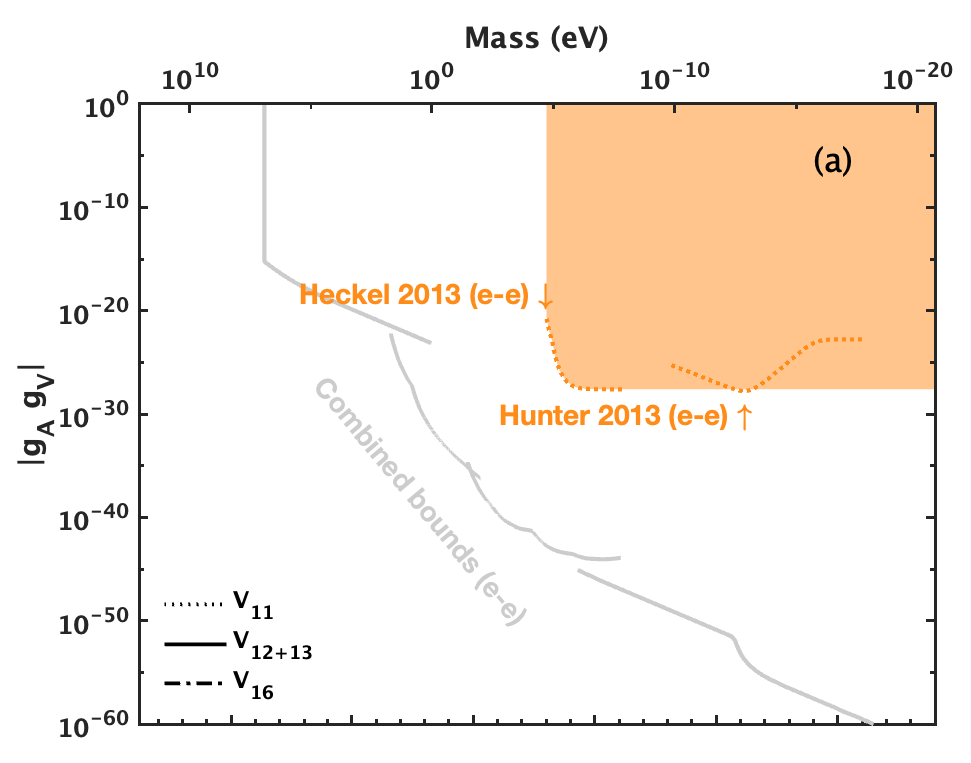
\includegraphics[width=0.48\textwidth]{Fig9_gAgV_a.eps}
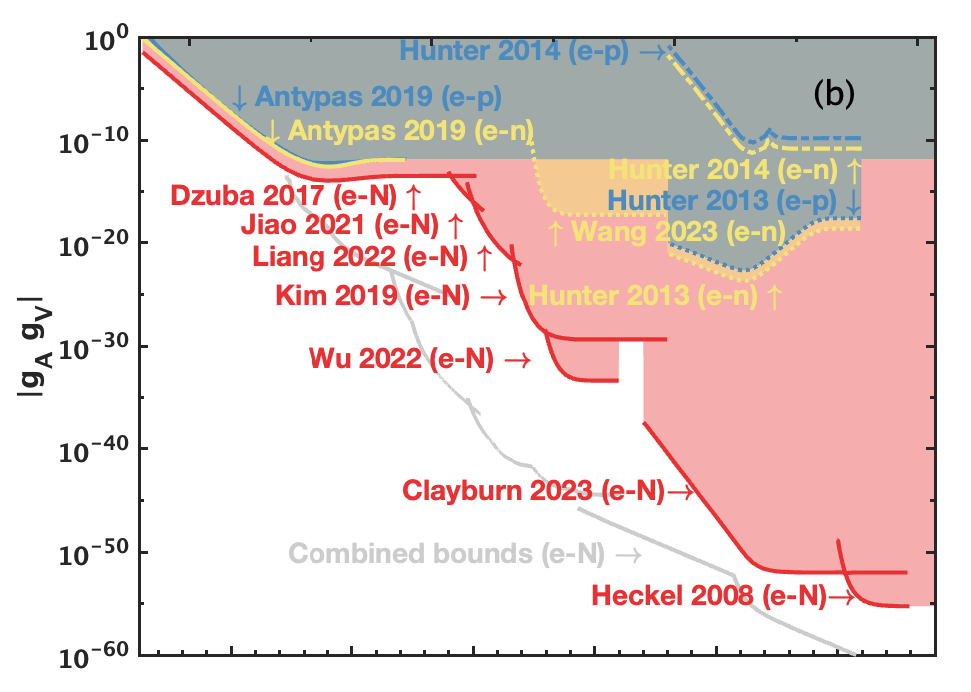
\includegraphics[width=0.48\textwidth]{Fig9_gAgV_b.eps}
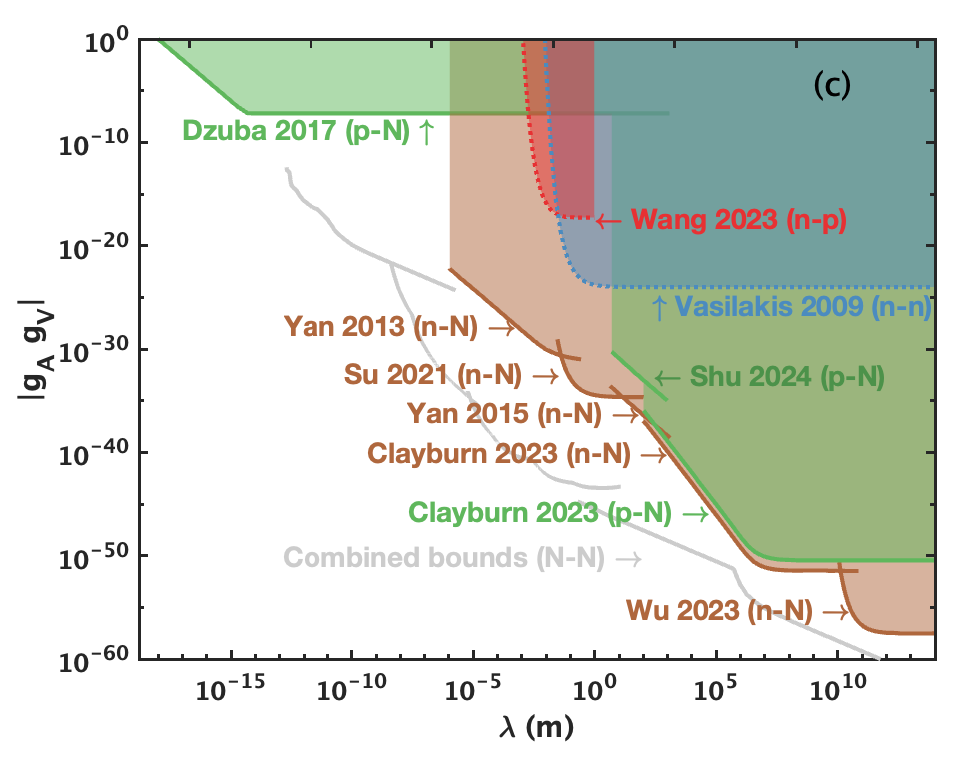
\includegraphics[width=0.48\textwidth]{Fig9_gAgV_c.eps}
\end{center}
\caption{
%\YS{{\color{red}Figure temporarily made in two-column format to make room for comments below. Please change back to single-column format when needed.}} 
Constraints, depicted by coloured regions, on the coupling constant product $g_A g_V$ as a function of the interaction range $\lambda$ shown on the bottom x-axis. 
The top x-axis represents the new spin-1 boson mass $M$. 
Here, the subscripts $A$ and $V$ denote the axial-vector and vector couplings, respectively. 
Constraints shown for \textbf{(a)} $e$-$e$, \textbf{(b)} $e$-$N$, \textbf{(c)} $N$-$N$ couplings. 
Results include $V_{11}$ (dotted line), $V_{12+13}$ (solid line), and $V_{16}$ (dash-dotted line) 
%\YS{Should we mention $V_{11p+16}$ here as well, or just leave as-is?}\LC{Maybe not mention, we have this in text.} \YS{OK}
terms. 
Combined bounds (faint, gray lines) are elaborated in Appendix\,\ref{appendix_comp.}. 
%\YS{Is it possible to adjust the positions of the arrows associated with the "Heckel 2013 ($e$-$e$)" curve in subfigure (a) and the "Hunter 2013 ($e$-$n$)" curve in (b) to be closer to their respective curves?} \LC{Done}
}
\label{gvga-fig}
\end{figure}


%\YS{For figure\,\ref{gvga-fig}. Points to check: 
%It's a bit unclear where the arrow of the Hunter 2013 (e-e) label points to. 
%The Hunter 2013 (e-n) bound looks a bit weaker than in the original paper. 
%\cite{hunter_using_2013} also gave bounds on e-p, n-e and p-e combinations. Should we show these in the figures and/or discuss in the main text?
%The Hunter 2014 (e-n) and (e-p) bounds look a bit weaker than in the original paper. 
%It looks like \cite{wang_search_2023} also set bounds on n-e and p-n combinations as well, correct? (Do we discuss the latter in the main text?)} 
%Please see my comments in the main text about the Vasilakis 2009 (n-n) bound.}\LC:done 
%\LC{We plot for $g_A g_V$ while their figure is for $g_V g_A$. So our e-n line corresponds to their n-e line. Same is true for Hunter 2014. I have add the e-p line from \cite{hunter_using_2013} in the figure. Constraints for e-p and p-e have a ratio of $m_e/m_p$, so we do not need to plot p-e and n-e results. \cite{wang_search_2023} also set constraints for n-e and p-n. However, these results can be obtained by simply make some transformation, therefore we do not choose to present them. In principle, all the other constraints can be transferred in the same way, right? If so, we may mention this in the Sec.\,\ref{Sec:limits_main_overview}.} 
%\YS{Thank you for clarifying, Lei! I think I more or less understand now. I agree that there's no need to plot the constraints for the ``permuted'' combinations. It would be nice to add a note here explaining that, e.g., for the $V_{11}$ term, it is possible to extract a bound on $g_A^X g_V^Y$ by simply multiplying the bound on $g_A^Y g_V^X$ by the fermion mass ratio $m_Y / m_X$.}
%\LC{Ok, I have added this in the end of the first paragraph of e-n subsection. It seems this is the single case for $V_{11}$ only.}
%\YS{{\color{red}[Update (12/04/2024)]: I have another related question -- Just to double-check my understanding: In Figure~\ref{gvga-fig}(b), do the two $V_{16}$-type Hunter 2014 curves contain a correction factor of $\sim m_N/m_e \sim 10^3$ [rather than $\sim (m_N/m_e)^2 \sim 10^6$]?}} \LC{[Update (13/04/2024)]Yes, you are right. For the data from their figure, we use a factor $m_N/m_e \times 8\pi$, and we assume Hunter 2014 missing a factor 1/c, otherwise the dimension is not correct. Also, we do not think Hunter 2014 give a correct $V_{16}$ potential form with different $M_1$ and $M_2$, see our Eq.\,\eqref{V16-V_AV}. This kind of translation relationship and typos, I do not plan to discuss in detail in our review, instead, they will be presented as notes together with the data in our ongoing Github webpage.}
%\YS{Thank you for explaining, Lei. One indeed gets a different conclusion for identical fermions if one uses Hunter 2014's form of $V_{16}$ instead of our Eq.\,\eqref{V16-V_AV}. And it looks like Hunter does have incorrect dimensions for their $V_{16}$ (missing factor of $\hbar$ in the numerator by the looks of things).} \LC{They plot with $g_Vg_A/(\hbar c)$, so in the end, they are missing a factor of $c$. }

%\YS{{\color{red} The ``Combined bounds (e-e)'' curve containing $g_V^e$ may need to be updated. Please see the discussion around Eq.~(\ref{gse-alpha}).}} \LC{Done.} \YS{Thank you for updating, Lei!} 

In the range of $\lambda$ around $\sim 0.1\,\textrm{m}$, the most stringent constraints on $g_A^eg_V^N$ are given by \citet{kim_experimental_2019} and \citet{wu_experimental_2022}. 
\citet{kim_experimental_2019} searched for the odd-parity spin- and velocity-dependent interaction term $V_{12+13}$ 
%performed with electron-spin-polarized torsion-pendulum experiments in \cite{heckel_preferred-frame_2008} 
by using
%\DKDel{a sensitive atomic magnetometer based on} 
an optically pumped alkali-metal atomic vapor
%\DKIns{
magnetometer
%} 
\cite{chu_search_2016}. 
%\YS{Similar to my question a couple of paragraphs above, how do we define improvement when we're talking about interactions on different scales? \LCa{I have updated the content above.} What type(s) of normalisation are involved/implied in the sensitivity measure?} 
%\YS{All good now, thank you!}
%The atomic magnetometer detects an effective magnetic field $B_\textrm{eff}$ produced by the interaction $V_{12+13}$ and operates in the SERF regime.
%in which the effects of spin-exchange collisions on spin relaxation are tuned off, dramatically improving the sensitivity to the femtotesla (f\,T) level. 
Their approach probes exotic interactions between optically polarized electrons in an atomic vapor and unpolarized or polarized particles of a solid-state mass in the vicinity of the atomic vapor. \citet{wu_experimental_2022} uses an array of atomic magnetometers instead of a single one in order to increase the statistics and cancel the common-mode noise. They use rotationally modulated source masses while the previously used unpolarized BGO mass in \citet{kim_experimental_2019} was translated up and down. This allows for removing possible slow drifts which enabled 
 an improvement by a factor of up to 20,000 on some of the limits on $g^e_ Ag^N_V$.

In the range of $\lambda$ around $10^{-5}$\,m, the most stringent constraints are given by \citet{jiao_experimental_2021}  and \citet{liang_new_2022} using NV center in diamonds. 
%They are based on a magnetometer with a single  and ensembles of such NV centers, respectively, see Sec.\,\ref{METH1.SENS.SS}. 
%Similar to the magnetometer of \citet{kim_experimental_2019}, the NV spin $\sigma$ is used to sense the effective magnetic field $B_\textrm{eff}$ produced by the %\LCa{exotic %} interaction %\YS{with what?} \LCa{between a polarized electron and unpolarized nucleons. 
%}. 
\citet{jiao_experimental_2021} use a magnetometer that is based on a single NV center which is located close to the surface of a diamond. 
The source mass is a half-sphere lens made of fused silica. 
The NV spin detects an effective magnetic field created by the exotic spin-dependent interaction resulting from the moving nucleons. 
%Due to the size of the sensor, which is small compared to the micrometer force range, the sensor and the source can be placed close to one another. Thus,
This experiment imposes constraints on the exotic spin- and velocity-dependent interaction within the force range of the order of $\sim 1-100$\,\textmu m. 
%\DK{This should definitely be ``range of the order of $\sim 1-100$\,$\mu$m'' correct?}\LC{Yes, thank you, I have corrected it.}
%1$\sim$100\,\textmu m. 
\citet{liang_new_2022} improved the magnetometer by using ensembles of NV centers in diamond yielding improved magnetic field sensitivity.
%, which enabled  more than three orders of magnitude improvement on the new interaction constraint at 330\,\textmu m. 
It is worth noting that \citet{ren_search_2021} employ a sensitive cantilever with a magnetic tip to directly measure the force between polarized electrons and unpolarized nucleons at this scale, and the obtained constraints approach the limits set with NV magnetometers.

Constraints at the shortest range are given by \citet{dzuba_probing_2017} by calculating PV effects in atoms and molecules (see Sec.\,\ref{METH2.PV}) which is induced by the exchange of vector bosons between electrons and nucleons. 
The vector-mediated atomic PV effect is calculated using the same relativistic many-body approaches as in earlier calculations of standard-model PV effects, but for the \YS{relativistic analogue of the more generic} operator $V_{12+13}$ instead. 
The detailed calculation starts with the relativistic Hartree-Fock-Dirac method, including electron-core polarization corrections calculated in the random phase approximation framework, followed by the use of either the correlation potential method or the combination of the configuration interaction and many-body perturbation theory methods, depending on the species of atoms. 
The obtained results for Cs, Yb, and Tl were used to constrain the parity-violating axial-vector/vector electron-nucleon interaction, while the determination of the nuclear anapole moment of $^{133}$Cs was used to constrain the parity-violating axial-vector/vector proton-neutron interaction. %\LC{ok}
Such interactions at the atomic and subatomic length scales allow one to effectively  %\LC{ok} 
probe larger boson masses compared to experiments using spin-polarized torsion pendula, atoms and NV centers %\YS{
that probe interactions at longer ranges.
%}. 
%probing longer ranges. 



%%%%
%\subsubsection{$e$-$n$}
\subsubsection{\texorpdfstring{$e$-$n$}{e-n}}
\label{g_Vg_A_e-n}

%\YS{Why do we discuss the electron-neutron case separately from the electron-nucleon case in Sec.\,\ref{Sec:A-V_e-N} above?}\LC{will make change}\YS{Thank you.} 

In the range $10^3 \, \textrm{m} < \lambda < 10^{11}$\,m, the most stringent constraints on the exotic axial-vector/vector interaction $g_A^e g_V^n$ between the particle pairs $e$-$n$ were obtained by \citet{hunter_using_2013} by investigating the $V_{11}$ term interaction between geoelectrons and neutrons in the sensor, as shown in Figure~\ref{gvga-fig}\,(b). 
Note that for the $V_{11}$ term, it is possible to extract a bound on $g_A^X g_V^Y$ by simply multiplying the bound on $g_V^X g_A^Y $ by the fermion mass ratio $m_Y / m_X$, see Eq.\,\eqref{pseudovector-vector_potential}.
%\citet{hunter_using_2013} examined possible exotic interactions of the type $V_{11}$ between spin-polarized geoelectrons and spin-polarized neutrons in the laboratory experiment. % \cite{venema_search_1992}. 
%\citet{hunter_using_2013} set the most stringent %\sout{long-range} 
%constraints on $g_A^eg_V^n$ in the range $10^{3}\,\textrm{m} <\lambda<10^{11}$\,m. 
%\YS{The last sentence in this paragraph looks like it is mostly repeating the first sentence.} 
%\YS{For which masses? \LC{in the range of $10^{3}<\lambda<10^{11}$\,m} I would avoid using the descriptor ``long-range'' here and in similar contexts elsewhere, since the concept of what is long-range and what is short-range depends on the size of the apparatus/phenomenon being considered. Indeed, almost all macroscopic-scale experiments are at their most sensitive for the boson masses when the potential is long-range on the scale of the experiment. There would be less ambiguity in stating the relevant mass range(s) instead.} 
%\LC{Ok, I have checked all other places that use long-range and modified them.}\YS{Thank you!}

In their next work, \citet{hunter_using_2014} investigated the velocity-dependent spin-spin interaction term $V_{16}$ using their model of the electron spins within Earth discussed in \citet{hunter_using_2013}. 
%Other experiments employ spin-polarized laboratory sources, with which it is difficult to constrain velocity-dependent interactions. 
%\YS{Are there simple reason(s) to understand why this is the case? Is it simply because the rotation of Earth provides a faster relative velocity than we can generate in the lab ourselves for macroscopic bodies? What about for microscopic particles?} \LCa{The original paper talks about that magnetometer and electron-spin polarized torsion pendulum experiments can not be used to study velocity-dependent interaction because on average, there is no relative velocity between the source and detection spins. So I suggest removing the sentence in question.}
%Until now, 
To date, \citet{hunter_using_2014} remains the only the paper to place constraints on $g_A^eg_V^n$ via the $V_{16}$ term. 
%\YS{Please see my comment/question about the contribution of $\mathcal{V}_{16}$ to the $A-V$ potential above.}\LCa{Ok, we resolve this once we decide on $V_{16}$.}
%\YS{I think it's okay to leave the text as-is here.}
Their latest work \citet{clayburn_using_2023} is based on these three related experiments (\citealp{venema_search_1992}; \citealp{heckel_preferred-frame_2008}; \citealp{peck_limits_2012}),
%\cite{peck_limits_2012,heckel_preferred-frame_2008,venema_search_1992}
but set constraints via the spin-velocity interaction $V_{12+13}$ and $V_{4+5}$. 
However, since some experiments have already been updated, e.g. \citet{zhang_search_2023} measured the ratio of nuclear spin-precession frequencies between $^{129}$Xe and $^{131}$Xe, setting a more stringent constraint on the coupling energy between a nucleon spin and gravity than \citet{venema_search_1992}, it would be an opportune time to update the results of \citet{hunter_using_2013}; \citet{hunter_using_2014}; \citet{clayburn_using_2023}
%\citet{hunter_using_2014, hunter_using_2013, clayburn_using_2023} 
in the near future.
%\YS{Maybe we could clarify (some of) the specific changes/updates that were made?}\LCa{yes, I have made changes in the above sentence.}\YS{OK.}



For the interaction range $3\times 10^{-3}\,\textrm{m}<\lambda<10^3$\,m,  \citet{wang_search_2023} set the most stringent constraint by investigating the odd-parity spin-spin interaction term $V_{11}$ induced by the exchange of a hypothetical spin-1 $Z'$ boson. 
They developed a technique based on a quantum spin amplifier 
%\cite{jiang_floquet_2021} 
(see Sec.\,\ref{METH1.SENS.AM.SMSA}) %\YS{{\color{red}This section hyperlink appears to be missing (or possibly changed).}}
%{\color{red}for particle physics research} 
to resonantly search for exotic interactions. 
%\YS{The inclusion of the phrase ``for particle physics research'' sounds a bit incoherent in this sentence. Unless we specifically want to emphasise the acronym SAPPHIRE = ``Spin Amplifier for Particle Physics REsearch'', it may be better to leave out this phrase.} \LCa{Ok!}
%The technique effectively amplifies the pseudomagnetic field generated by exotic interactions by a factor of about 200 while being insensitive to spurious external magnetic fields. Two polarized objects are typically placed close to one another in experimental searches for exotic spin-spin interactions, with one serving as a magnetic detector (or ``spin sensor'') to measure the exotic field generated by the other polarized object (or ``spin source''). 
In this experiment, the spin source uses polarized electron spins from $^{87}$Rb atoms, while the spin sensor uses polarized neutron spins from isotopically enriched polarized $^{129}$Xe gas. 
%Because of the significant Fermi-contact amplification factor for the magnetic dipole-dipole interaction, 
%\YS{for the magnetic dipole-dipole interaction}\LC{ok}, 
%\textit{in-situ} measurements have the advantage of enhancing nuclear resonance signals. 
%This work bridges the gap between Earth-scale \cite{hunter_using_2013} and atomic-scale \cite{antypas_isotopic_2019} experiments using a centimeter-scale detection technique. 
%spins that function as an in-situ magnetometer cost $^{87}$Rb.

In the range $2.1\times10^{-19}\,\textrm{m} < \lambda < 3 \times10^{-3}$\,m, \citet{antypas_isotopic_2019} use isotopic comparison data 
%\YS{
in APV experiments
%}
to provide the most stringent individual constraints on the electron–neutron interaction %\YS{
via \YS{the relativistic analogue of} the $V_{12+13}$ term. 
%}. 
\citet{antypas_isotopic_2019} provide a measurement of the APV effect in four nuclear-spin-zero isotopes of Yb, namely $^{170}$Yb, $^{172}$Yb, $^{174}$Yb and $^{176}$Yb (see Secs.\,\ref{METH2.PV}). % and \ref{METH2.IS}). %\LC{should we mention this work in Sec.\,\ref{METH2.IS}?} \YS{Technically, Sec.\,\ref{METH2.IS} discusses isotope shifts in a different context of spectroscopy measurements, but it may be a good idea to also discuss APV measurements briefly there as well.} 
Such an isotopic variation in atomic parity violation confirms the predicted SM weak nuclear charge ($Q_\textrm{W}$) scaling with the number of neutrons, and also offers information about an additional $Z'$ boson. 
This is similar to the earlier result of \citet{dzuba_probing_2017}, which combined new atomic calculations with experimental data from previous APV experiments to place constraints on $g_A^e g_V^N$. 
%use atomic calculations use the results of previous atomic PV experiments. 
%In fact, here \citet{antypas_isotopic_2019} consider the PV effects arising from the exchange of a vector boson $Z'$ between the electrons and nucleons also in the form of the $V_{12+13}$ interaction like in \citet{dzuba_probing_2017}. 
The interaction effectively modifies the SM weak charge: $Q_\textrm{W} = Q_\textrm{W}^\textrm{SM} + Q_\textrm{W}^\textrm{exotic}$, with 
%\YS{
the former term being approximately proportional to the number of neutrons and the latter term being proportional to $g_A^eg_V^N$. 
%\citet{antypas_isotopic_2019} use their data for the observed proton contribution to the PV amplitude to constrain $g_A^eg_V^p$. 
These bounds are then combined [through Eq.\,(10) in their paper] with constraints on the effective $g_A^e g_V^N$ coupling that come from the %{\color{red}
analysis of the Cs PV results in \citet{wood_measurement_1997} to give limits on the electron–neutron interaction $g_A^e g_V^n$. 
%}
%\YS{I'm not sure what we're trying to say in this sentence.} \LC{It is like they have the result of $g_A^eg_V^p$ and $g_A^eg_V^N$, and by calculation, they got $g_A^eg_V^n$.}
%\YS{I see. 
%I think the caveat here is that in order to derive a limit on $g_A^e g_V^n$ in this way, one requires a limit on $g_A^e g_V^p$ that is much better than the limit on $g_A^e g_V^N$, or to have a nonzero result for one of $g_A^e g_V^p$ or $g_A^e g_V^N$. 
%Is this correct?}\LCa{I'm not sure. We could check the content around Eq. (10) in \citet{antypas_isotopic_2019}, however, it is not straightly mentioned there. Perhaps we should check the numbers to see if this is true.}



%%%%
%\subsubsection{$e$-$p$}
\subsubsection{\texorpdfstring{$e$-$p$}{e-p}}
As shown in Figure\,\ref{gvga-fig}\,(b) and discussed in Sec.\,\ref{g_Vg_A_e-n}, \citet{antypas_isotopic_2019} also provide the constraints on the electron-proton interaction via the potential term $V_{12+13}$ over the range $\lambda>3.9\times10^{-19}$\,m. 
In the range $10^3 \, \textrm{m} < \lambda < 10^{11}$\,m, the most stringent constraints on $g_A^e g_V^p$ were obtained by \citet{hunter_using_2013}. 
In addition, \citet{hunter_using_2014} also investigated the velocity-dependent spin-spin potential term $V_{16}$ 
%\YS{Please see my comment/question about $\mathcal{V}_{16}$ above.} 
and provided constraints on the electron-proton potential over the range $\lambda>1.1\times10^{-3}$\,m. 


%%%%
%\subsubsection{$n$-$N$}
\subsubsection{\texorpdfstring{$n$-$N$}{n-N}}
% \YS{Does the $(+e)$ here mean $n$-$e$? Maybe it would be clearer to write $n$-$N$ (and $n$-$e$) in that case?} It is for $n$-$N+e$, \citet{yan_new_2013} set constraints between n and n+p+e. We may explain this in the main text. }
Figure~\ref{gvga-fig}\,(c) shows the most stringent constraints on the exotic axial-vector/vector interaction $g_A^n g_V^N$ between the particle pair $n$-$N$. 

%For the force range $>1.3\times10^{10}$\,m, \cite{wu_new_2023} analyzing existing data from laboratory measurements on Lorentz and CPT violation to derive upper limits on exotic spin-dependent interactions induced by the Sun and the Moon as source masses and Earth's rotation as a modulation. \cite{wu_new_2023} explores the possibility of exotic spin-dependent interactions involving scalar/pseudoscalar couplings, as well as vector/axial-vector couplings, mediated by new particles. 

At the astronomical distances $\lambda > 1.3\times 10^{10}$\,m, \citet{wu_new_2023} analysed existing data from laboratory measurements (\citealp{brown_new_2010}; \citealp{allmendinger_new_2014})
%\cite{allmendinger_new_2014, brown_new_2010} 
on Lorentz and $CPT$ violation to derive upper limits on exotic spin-dependent interactions of the form $V_{12+13}$ induced by the Sun (or Moon) as source masses and Earth's rotation as a modulation. 
\citet{brown_new_2010} and \citet{allmendinger_new_2014} originally searched for a sidereal signal induced by a Lorentz-Invariance- and $CPT$-violating background field.
\citet{wu_new_2023} explored the possibility of exotic spin-dependent interactions involving axial-vector/vector couplings $g_A g_V$, as well as axial-vector/axial-vector couplings $g_A g_A$ and pseudoscalar/scalar couplings $g_p g_s$, mediated by new particles. %Searching for these interactions is considered a problem probing the effective field acting on the polarized spin by dual-species comagnetometers. \citet{allmendinger_new_2014, brown_new_2010} has applied comagnetometer method to search for the constant cosmic background field due to Lorentz violation by detecting the sidereal variants of the field. 
%By using the results for the Sun \cite{allmendinger_new_2014} 
%\YS{Did \cite{allmendinger_new_2014} specifically look for Sun-induced signals? I seem to recall that they looked for sidereal signals. Maybe worth clarifying or rewording?}\LCa{yes, you are right. We can rewrite as suggested, see below: } %\YS{OK now.}
%\LC{Remove, kind of repeate: \citet{wu_new_2023} reanalysed the data of \citet{brown_new_2010} and \citet{allmendinger_new_2014}, which were originally used to search a sidereal signal induced by a Lorentz-Invariance- and $CPT$-violating background field, to search for exotic interactions sourced by the Sun and Moon.} 
%\citet{wu_new_2023} obtained limits on exotic spin-dependent that are 12 orders of magnitude improved compared to the earlier bounds in \citet{yan_searching_2015}. 
%\citet{wu_new_2023} also performed a similar analysis using the Moon as a source \cite{brown_new_2010} \YS{A similar question here: Maybe it would be clearer to say something along the lines of ``\citet{wu_new_2023} reanalysed the data of \cite{brown_new_2010}, which were originally used to search a sidereal signal induced by a Lorentz- and \textit{CPT}-violating background field, to search for exotic interactions sourced by the Moon''?} \LCa{yes}, but these constraints have since been surpassed by \citet{clayburn_using_2023}. 

For the interaction range $10^{2}\,\textrm{m} < \lambda < 1.3 \times 10^{10}$\,m, \citet{clayburn_using_2023} utilized data from the 
%the torsion-pendulum experiment results of \cite{heckel_preferred-frame_2008} 
%\LC{
$^{199}$Hg-$^{133}$Cs comagnetometer experiment (\citealp{peck_limits_2012}; \citealp{hunter_using_2013})
%\cite{peck_limits_2012,hunter_using_2013}
%}
and the Earth model (\citealp{hunter_using_2013}; \citeyear{hunter_using_2014})
 to set the most stringent constraints on $g_A^ng_V^N$ via the $V_{12+13}$ term. 
%, see Sec.\,\ref{Sec:A-V_e-N}. 
%\YS{Sec.~\ref{Sec:A-V_e-e}?} 
%\YS{I'm confused here. The paper \cite{heckel_preferred-frame_2008} used a spin pendulum with spin-polarized electrons. Earth contains spin-polarized geoelectrons. How do we get limits on $g_A^ng_V^N$ (which requires spin-polarized neutrons) in this case?} \LC{Your concern is right. I corrected to $^{199}$Hg-$^{133}$Cs comagnetometer experiment.}\YS{OK. Thank you for checking and updating!}

For the force range $6\,\textrm{m} < \lambda < 10^2$\,m, \citet{yan_searching_2015} used the best available $T_2$ measurement of polarized $^3$He gas atoms as the polarized sensor and Earth as an unpolarized source to present the most stringent experimental upper bound on $g_A^n g_V^N$. 
The physical effects of $V_{12+13}$ were considered to produce a velocity-dependent pseudomagnetic field, 
%\YS{
fluctuations in which would change the spin relaxation time of the $^3$He nuclear spins.
%} 
%and as a fluctuating magnetic field, it changes the spin relaxation time. 
Thus it is possible to detect or constrain new physics by measuring the longitudinal spin relaxation time ($T_1$) or the transverse relaxation time ($T_2$) of polarized noble gases 
(\citealp{pokotilovski_limits_2010}; \citealp{petukhov_polarized_2010}; \citealp{fu_limits_2011}).
%\cite{pokotilovski_limits_2010,petukhov_polarized_2010,fu_limits_2011}. 
%\YS{Did \cite{moody_new_1984} specifically discuss the use of relaxation time measurements to probe new forces? I recall that they discussed mechanical-type force sensors. They do discuss the relaxation times of these mechanical systems, but it appears to be more from the point of view of wanting to maximise the Q-factors of the systems to have better force sensors. Is there something that I missed?} \LC{They mentioned around the oscillators part "However, if a measurement sensitivity of 10 cm/sec were attained, the entire suggested range in 0 for the axion monopole-dipole force could be tested." They also have the relaxation time in and around their Eq. 27. However, if we have concerns, we can remove \cite{moody_new_1984} here.}
%\YS{I had another look at the \cite{moody_new_1984} paper. It looks like the relevant observable there is acceleration. The discussion of $Q$-factors there is related to wanting to have high $Q$ factors for experiments to improve the acceleration sensitivity. I would propose to simply remove the \cite{moody_new_1984} reference from the list here.} 
%To have sensitive NMR measurements of spin dynamics and to obtain the relaxation time needed for this search, an ensemble of polarized gases with large phase space densities of polarized probe particles is used. 
Since the noble gas is sealed in a still glass cell, $\langle \v v \rangle$ is zero, but $\langle v^2 \rangle$ is not. 
The nonzero $\langle v^2 \rangle$ produced by the velocity-dependent pseudo-magnetic field changes the spin relaxation times of polarized noble gases. 
Thus, although there is no bulk motion of either the polarized or unpolarized masses in the experiments, it is still possible to constrain the velocity-dependent interactions $V_{12+13}$.
%the limit is improved by about sixteen orders of magnitude compared with the previous result of the neutron spin rotation experiment \cite{yan_new_2013}. 
%\YS{Why is the distance / interaction range of $\sim 10^8$ m important here? We don't show either the bounds from \cite{yan_searching_2015} or \cite{yan_new_2013} for this range of $\lambda$ in the relevant figure. Over the shorter interaction ranges shown in the figure, the result of \cite{yan_searching_2015} is about 3-5 orders of magnitude more stringent than that of \cite{yan_new_2013}.} \LCa{The authors claim they set new constraints between 1-10$^8$ m, and there their result converge and is sixteen orders better.}\YS{OK}

%It is worth noting that besides the direct constraint on $|g_Ag_V|$ from a single experiment as shown above, \DKDel{substantially tighter} \DK{Looking at the literature I don't think these limits are actually tighter than \citet{clayburn_using_2023}} limits on several closely related quantities \DK{What does ``closely related'' mean? Too vague.} can be found by combining bounds on $|g^n_A|^2$ and on $|g_V|^2$ set by previous experiments to obtain bounds on $|g^n_Ag^N_V|$, see \citet{adelberger_improved_2013,yan_searching_2015}. \DKDel{\citet{yan_searching_2015} set orders of magnitude better constraints than \citet{adelberger_improved_2013} for $\lambda \sim 10^8$\,m.} \DK{This last sentence comes out of the blue and really confuses the reader. First, the constraints from \citet{yan_searching_2015} don't extend on the plot to the longer range ($\lambda \sim 10^8$\,m) discussed. Second, the constraints from \citet{adelberger_improved_2013} don't appear on the plot at all. I went back to the original literature to try to figure out what you're saying. I understand now but given what is presented the statement has absolutely no context for the reader. Since all of the discussed limits have been superseded by the work of \citet{clayburn_using_2023}, I recommend we just delete this last sentence, and maybe the sentence before that.}\LC{I remove two of the sentences. If they cause confusion, we'd better not present them.}

%\YS{For which interaction parameter(s) and interaction range? (I don't see the comparison bounds in the figure.)} \LCa{didn't present to avoid overcrowding.}\YS{OK}


For the interaction range $0.05\,\textrm{m} < \lambda < 6$\,m, the most stringent constraints \cite{su_search_2021} come from measurements using a spin-based amplifier (see Sec.\,\ref{METH1.SENS.AM.SMSA}) to search for effects due to pseudomagnetic fields associated with the interaction term $V_{12+13}$ between polarized neutrons and unpolarized nucleons. 
In their experiment, the polarized 
%\LC{yes}
neutrons are mainly from $^{129}$Xe (where 73\% of the nuclear spin is due to neutron spins)
% \YS{73\% of what? Is this polarization fraction or another quantity?} \LC{The 73\% refers to the predicted or observed fractional contribution of neutron spins to the overall magnetic properties of $^{129}$ Xe. And 27\% is from proton.} \YS{OK, understood. I've updated the phrase. Please check to see if this is okay.}) 
and the source of unpolarized nucleons is mainly from a high density BGO crystal.% with a high number density of nucleons. 
%The spin-based amplifier refers to hyperpolarized nuclear spins consisting of the spatially overlapping ensembles of spin-polarized $^{87}$Rb and $^{129}$Xe and it can offer amplification of more than 100 times. This technique takes advantage of the resonant coupling between the rotation frequency of an unpolarized mass and a spin-based amplifier with a matching spin-precession frequency.

%In contrast to the previous NMR searches (proposals), which also use resonance methods \cite{arvanitaki_resonantly_2014, chu_search_2020},
%\YS{\cite{arvanitaki_resonantly_2014} was only a proposal rather than an experimental search}, 
%\citet{su_search_2021} employ a scheme where polarized nucleons and the alkali atom are spatially overlapped in the same vapor cell, providing two significant advantages: first, nuclear spins can be hyperpolarized %\sout{in place}
%\textit{in situ}, 
%\YS{in-situ?}\LC{yes}
%which reduces polarization loss during transport to the detection region; second, nuclear spin signals are enhanced due to the Fermi-contact interaction and can be measured \textit{in-situ} with the alkali-atom-based atomic magnetometer. 

For the force range $10^{-6}\,\textrm{m} < \lambda < 0.05$\,m, the most stringent constraints on $g_A^n g_V$ come from a cold neutron beam experiment \cite{yan_new_2013} (see Sec.\,\ref{METH1.SENS.PBS}.). 
%\YS{ which specific material(s)?} \LC{in this experiment, they use liquid $^4$He.}, 
\citet{yan_new_2013} derived an upper bound on the product of couplings $g_A^ng_V$ %\YS{, where $g_V=2g_V^p+2g_V^n+2g_V^e$ {\color{red}
[the definition of $g_V$ is discussed below Eq.\,\eqref{ANZ}] %- should we keep the part in parentheses here?},}\LC{how about we do not repeat the equation here, but direct the reader to the discussion below Eq.~(\ref{ANZ})?} \YS{OK}
in the mesoscopic range based on their prior experiments with neutron spin rotation in liquid $^4$He \cite{snow_upper_2011}. 
\citet{yan_new_2013} take advantage of the fact that the interaction potential proportional to $\boldsymbol{\sigma}\cdot\boldsymbol{v}$ violates parity and, as a result, when slow neutrons pass close to the surface %of a plane 
of an unpolarized bulk material, the exotic interaction causes a rotation of the plane of polarization, which can be measured using the separated oscillating fields method \cite{ramsey_molecular_1950}. 
%\citet{yan_new_2013} demonstrated that slow neutron spin rotation is a very sensitive method to search for exotic interactions of neutron spins that violate parity, with seven orders of magnitude more stringent limits than the previous laboratory constraints of length scales below 1 m \cite{vasilakis_limits_2009}. 
%\YS{What were the previous experimental results? Maybe add a brief description and reference(s)? In which interaction range is this comparison in sensitivity for?} \LCa{added}


In addition, there are also two sets of constraints on the neutron-nucleon interaction derived from the odd-parity spin-spin interaction term $V_{11}$. 
\citet{vasilakis_limits_2009} presents limits on the neutron-neutron coupling $g_A^ng_V^n$ in the limit of a massless spin-1 particle to be $9.8\times 10^{-25}$ 
%\YS{In Table I, \citet{vasilakis_limits_2009} gives the bound $|g_A g_V|/(4\pi) < 3.9 \times 10^{-26}$. Is this consistent with the quoted value here?}\LC{yes, we recalculate from the data in Table I.} \YS{I think I understand now. \citet{vasilakis_limits_2009}'s Eq.~(5) is bigger by a factor of 2 compared to our Eq.~(\ref{pseudovector-vector_potential}), correct?}\LC{yes}
[represented in Fig.\,\ref{gvga-fig}(c)]. 
%\YS{I think the meaning of massless limit is taken too literally in Fig.~\ref{gvga-fig}(c). Massless limit is a convenient limiting case of boson masses when $Mr \ll 1$, which allows the authors to tabulate bounds that they don't otherwise have space to present in figures. Looking at the structures of Eqs. (3), (4) and (5), the dimensions of the apparatus and Figure 4 in \citet{vasilakis_limits_2009}, one can conclude that their bounds on $g_A g_V$ and $g_A^2$ in Table I apply to all boson masses $M \lesssim 10^{-7}$\,eV. Why not present bounds in Fig.~\ref{gvga-fig}(c) up to these masses instead of presenting a single point that is outside of the plot range?} \LCa{Ok, then we include the two lines in our figure, the $|g_A g_V|$ has been plotted in \citet{yan_new_2013}'s Fig.\,2.} \YS{Super, thank you!}
%\LC{Shouldn't we use citet instead of cite here? And use present not presents.}
%\YS{I've seen both citet and cite used throughout the review. It would be nice to standardise to one form or the other. I think it's possible to do this using the search and replace for all instances function on Overleaf. }\LC{There are slight differences between the two usages. If the literature serves as elements of the sentence, then we use citet; If it is a traditional citation, then we use cite. }
%\YS{Thank you for clarifying.}
%Here we extend this result to $10^{10}$\,m with the (blue) filled area. 
%\YS{Why stop at $10^8$\,m here? We can in principle extrapolate to infinite range here, since the form of the potential practically doesn't change at these length scales (equivalently boson masses).} 
%\LC{This is a typo here, we extend the result from the left part of the figure to right and $10^{10}$ is where meets the limits given by \citet{yan_searching_2015}. I plan to make a change here, using an arrow to indicate the result of \cite{vasilakis_limits_2009}, as the Fig.\,\ref{gaga-fig}(d). }\YS{OK, thank you for clarifying.}
Further description of the experiment \citet{vasilakis_limits_2009} can be found in Sec.\,\ref{subsec_g_Pg_P}, as it gives the most stringent constraint on $g_p g_p$ for the lightest boson masses. 
%\YS{for the lightest boson masses. }\LC{ok}
%in the long-range there. 
For the force range $10^{-3}\,\textrm{m} < \lambda < 1$\,m, \citet{wang_search_2023} set the most stringent constraints on the odd-parity spin-spin interaction $V_{11}$. 
The authors consider valence protons within the Rb nuclei as %\YS{as?}\LC{yes} 
the spin source. 
Further details about \citet{wang_search_2023} can be found in Sec.\,\ref{g_Vg_A_e-n}. 



%%%
%\subsubsection{$p$-$N$}
\subsubsection{\texorpdfstring{$p$-$N$}{p-N}}
%`\YS{A similar comment to earlier --- Why do we have e-p separate from the e-N and e-n sections? Also, why is p-N separate from the n-N section?}\LC{will change soon.}
%\YS{Thank you! I just had the following thought: If we group interactions according to leptonic/semi-leptonic/hadronic classification in the summary plots, could we in principle do the same in the main text?} \LC{Yes, we will do the same in the main text. Here, we have a problem because sometimes, one of the subfigures may be too crowded and I may consider separating it to be two. Otherwise, we make such a subfigure bigger as a full column wide.}

As shown in Figure~\ref{gvga-fig}\,(c), \citet{dzuba_probing_2017}; \citet{clayburn_using_2023}
%\citet{clayburn_using_2023,dzuba_probing_2017} 
also set limits on proton-nucleon ($p$-$N$) interactions via the term $V_{12+13}$ mediated by a vector boson. For further details of these searches, see Sec.\,\ref{Sec:A-V_e-N}. In addition, \citet{shu_constraint_2024} set the best constraints for the force range $5\,\textrm{m} < \lambda < 100\,\textrm{m}$ by introducing the Bragg atom interferometer, loaded with $^{87}\textrm{Rb}$ atoms, as a novel type of spin sensor. The mountains surrounding their cave laboratory serve as the source of unpolarized nucleons. The atom interferometer holds potential for testing other exotic interaction terms, such as $V_{9+10}$ \cite{abe_search_2024} and $V_3$.


%%%
\subsubsection{Future perspectives}

There are many intriguing possibilities for the field of probing axial-vector/vector couplings in the future.

One of the promising directions involves the application of NV-center-based sensors (see Sec.\,\ref{METH1.SENS.SS.NV}) for micrometer-scale experiments, where the exotic interaction between the polarized electron spin and a moving nucleon source can be explored by measuring the %possible 
induced magnetic field experienced by the electron spin quantum sensor \cite{jiao_experimental_2021,liang_new_2022}. 

In particular, \citet{chu_proposal_2022} have proposed a new method to probe spin-dependent interactions based on NV centers in diamond. The experimental setup involves a spin source or mass source 
%spin source/mass source 
attached to a mechanical oscillator above the NV sensor, similar to that in \citet{rong_searching_2018}. 
However, they employ multipulse quantum sensing protocols, including the XY8-N sequence \cite{smits_two-dimensional_2019,glenn_high-resolution_2018}, to improve the sensitivity. 
\citet{chu_proposal_2022} analyzed two exotic spin-velocity interactions ($V_{12+13}$ and $V_{4+5}$) and three velocity-dependent spin-spin interactions ($V_{6+7}$, $V_{14}$, and $V_{15}$), 
%\YS{
and in all cases predict better sensitivity than existing experimental results over certain microscopic ranges (and in some cases, over certain macroscopic ranges as well). 
%} 
%all of which predict better constraints than existing experiment result. 


In addition, \citet{chu_proposal_2022} also identified a new spin source based on hyperpolarized $^{13}$C nuclear spins in a thin diamond membrane. 
This material offers the advantages of high spin polarization efficiency and low stray magnetic fields due to the small magnetic moment of $^{13}$C and the particular membrane geometry used. 

Also noteworthy are 
%a series of ``couch research'' \YS{Is it possible to use a different description here? Some of the authors mentioned in this paragraph may be offended by this label.} \LCa{This is a word Dima like to use, if it is not widely accepted, we can use ``theoretical exploration'' or ``Desktop physics''. }\YS{What about the following wording? ... 
a series of reinterpretations of existing older datasets.
%, wherein existing experimental and/or theoretical results available in the literature are further studied. 
For instance, \citet{clayburn_using_2023} utilized the torsion-pendulum experiment results of \cite{heckel_preferred-frame_2008} and the model of geoelectrons described in \citet{hunter_using_2013} and \citet{hunter_using_2014} to obtain new constraints on $V_{12+13}$ and $V_{4+5}$. 
\citet{wu_new_2023} reinterpreted the Lorentz and $CPT$ violation results in (\citealp{brown_new_2010}; \citealp{allmendinger_new_2014})
%\cite{allmendinger_new_2014,brown_new_2010} 
to place new bounds on the exotic spin-dependent interaction terms $V_{12+13}$, $V_{4+5}$ and $V_{9+10}$. 
Additionally, new atomic/molecular spectroscopy data could be used to set new and improved limits on exotic spin-dependent interactions. 
For example, \citet{antypas_isotopic_2019} studied vector-mediated PV effects in Cs, Yb and other elements, and set the most stringent constraints on atomic and subatomic length scales. 
%in the range around atomic and subatomic scale. 
Similarly, the ongoing experiments about Ra$^+$ ion \cite{nunez_portela_towards_2013} and Fr (\citealp{dzuba_calculation_1995}; \citealp{safronova_high-precision_2000}; \citealp{dzuba_calculations_2001}; \citealp{dzuba_calculation_2011-1}; \citealp{tandecki_offline_2014}) by the Manitoba-TRIUMF-Maryland team (\citealp{aubin_frpnc_2012}; \citealp{aubin_atomic_2013}),
%\cite{hucko_measurement_2023}
%\VF{references to published papers look better than to unpublished PhD thesis:  Atomic Parity Non-Conservation in Francium: The FrPNC Ex-periment at TRIUMF. S Aubin, E. Gomez, J. A. Behr, M. R. Pearson, D. Sheng, J. Zhang, R. Collister, D. Melconian, V. V. Flambaum, G. D. Sprouse, L. A. Orozco, and G. Gwinner. Nuovo Cimento della Societa Italiana di Fisica C 35(4):85-90 Jul 2012. Atomic parity non-conservation; the francium anapole project of the FrPNC collaboration at TRIUMF. S. Aubin J. A. Behr R. Collister V. V. Flambaum E. Gomez G. Gwinner K. P. Jackson D.Melconian L. A. Orozco M. R.Pearson D. Sheng G. D. Sprouse M. Tandecki J. Zhang Y. Zhao, Hyperfine interactions 214, 163-171 (2013).}\LC{Thanks, Victor. I have replaced them.}
%\VF{If appropriate, you may also include some of these references: Calculation of energy levels, E1 transition amplitudes and parity violation in francium. V. A. Dzuba, V. V. Flambaum, and O. P. Sushkov, Phys. Rev. A 51, 3454-3461 (1995). Calculations of parity nonconserving s-d transitions in Cs, Fr, Ba+, and Ra+ . V.A. Dzuba, V.V. Flambaum, and J.S.M. Ginges, Phys. Rev. A 63, 062101 (2001). Calculation of nuclear-spin-dependent parity nonconservation in s-d transitions of Ba+, Yb+ and Ra+ ions, V.A. Dzuba, V.V. Flambaum, arxiv:1104.0086 Phys. Rev. A83, 052513 (2011))} \LC{Thanks, cited.}
as well as other future PV experiments with atoms (\citealp{williams_method_2013}; \citealp{leefer_towards_2014}) and molecules (\citealp{isaev_laser-cooled_2010}; \citealp{cahn_zeeman-tuned_2014}) are expected to prompt the exploration of new forces. 
%; \citealp{hao_nuclear_2020}) LC: This Hao reference have some problem 
%\VF{New molecular experiment proposal:Nuclear spin-dependent parity-violating effects in light polyatomic molecules. Yongliang Hao, Petr Navratil, Eric B. Norrgard, Miroslav Iliaˇs,Ephraim Eliav, Rob G. E. Timmermans, Victor V. Flambaum, and Anastasia Borschevsky, Phys. Rev. A 102, 052828 (2020).  DOI: 10.1103/PhysRevA.102.052828} 

%\LC{
Recently, it was pointed out that neutrino-oscillations experiments can be interpreted as a probe for axial-vector/vector interactions of leptons and nucleons \cite{fang_testing_2024} as such interactions can influence neutrino oscillations. The analysis of current neutrino-oscillation experiments appears to yield competitive sensitivity to the coupling constants. 
%}






%%%%%%%%%%%%%%%%%%%%%%%%%%%%%%%%%%%%%%%%%%%%%%%%%%%%%%
                      % R2. g_A^2
%%%%%%%%%%%%%%%%%%%%%%%%%%%%%%%%%%%%%%%%%%%%%%%%%%%%%%


%%%
\subsection{Axial-vector/Axial-vector interaction \texorpdfstring{$g_Ag_A$}{gAgV}  }
\label{subsec_g_Ag_A}

Experimental constraints on the exotic axial-vector/axial-vector combination of parameters $g_A g_A$ can be derived from the potential terms $V_{2}$, $V_{3}$, $V_{4+5}$ and $V_{8}$ [see Eq.\,(\ref{pseudovector-pseudovector_potential})]: 
\begin{equation}
\label{gaga_V2}
\begin{aligned}
V_{2}=-g_A^Xg_A^Y \frac{\hbar c}{4\pi}\boldsymbol{\sigma}_X\cdot\v\sigma_Y^{\,\prime}\frac{1}{r}\,e^{-{r}/{\lambda}} \,.
\end{aligned}
\end{equation} 


%$V_{3}|_{AA}$ from Eq.\,\eqref{pseudovector-pseudovector_potential} is 
\begin{widetext}
\begin{equation}
\label{gaga_V3}
\begin{split}
V_{3}|_{AA}
%&=- g_A^X g_A^Y \frac{\hbar^3}{c} m_X m_Y \lambda^2  \left[ \v{\sigma}_X \cdot \v{\sigma }_Y \left( \frac{1}{r^3} + \frac{1}{\lambda r^2} + \frac{4 \pi}{3} \delta(\v{r}) \right)  -  \left( \v{\sigma}_X \cdot \hat{\v{r}} \right) \left( \v{\sigma }_Y \cdot \hat{\v{r}} \right)  \left( \frac{3}{r^3} + \frac{3}{\lambda r^2} + \frac{1}{\lambda^2r} \right)  \right] \frac{e^{-r/\lambda}}{4 \pi m_X m_Y}\,\\
%=&- \hbar c \frac{g_A^X g_A^Y m_X m_Y}{ (\frac{c}{\hbar})^2 M^2}  \left[ \v{\sigma}_X \cdot \v{\sigma }_Y \left[ \frac{1}{r^3} + \frac{\frac{c}{\hbar}M}{r^2} + \frac{4 \pi}{3} \delta(\v{r}) \right]  \right. \\
%&\left.-  \left( \v{\sigma}_X \cdot \hat{\v{r}} \right) \left( \v{\sigma }_Y \cdot \hat{\v{r}} \right)  \left( \frac{3}{r^3} + \frac{3\frac{c}{\hbar}M}{r^2} + \frac{(\frac{c}{\hbar})^2M^2}{r} \right)  \right] \frac{e^{-\frac{c}{\hbar}M r}}{4 \pi m_X m_Y}\,\\
= - \hbar c {g_A^X g_A^Y \lambda^2}  \left[ \v{\sigma}_X \cdot \v\sigma_Y^{\,\prime}\left[ \frac{1}{r^3} + \frac{1}{\lambda r^2} + \frac{4 \pi}{3} \delta(\v{r}) \right] -  \left( \v{\sigma}_X \cdot \hat{\v{r}} \right) \left( \v\sigma_Y^{\,\prime}\cdot \hat{\v{r}} \right)  \left( \frac{3}{r^3} + \frac{3}{\lambda r^2} + \frac{1}{\lambda^2 r} \right)  \right] \frac{e^{-r/\lambda}}{4 \pi}\,,
\end{split}
\end{equation}


%Note that the equation in (\ref{gaga_V3_initial}) is qualitatively very different from $V_{3}|_{AA}$ in Eq.\,\eqref{gaga_V3}. This is presented in \citet{fadeev_revisiting_2019,fadeev_pseudovector_2022} and especially addressed in the later. The point is that the $V_{3}|_{AA}$ contribution to the $A-A$ potential diverges with the mediator mass $M$ as $\propto 1/M^2$ as $M \to 0$ due to the non-conservation of the axial-vector current. ${g_A^X g_A^Y}=\frac{\hbar^2}{8 c^2}\frac{m_X^2+m_Y^2}{m_X^2 m_Y^2} \frac{1}{\lambda^2} {g_A^Xg_A^Y}_{initial}$. This has a major effect on the landscape of constraints presented in Fig.\,\ref{gaga-fig}.

% comments below has been modofied to be content above
%\YS{I have the same comments here as in the relevant place in the previous section above. Also, please note that the equation in (\ref{gaga_V3}) is qualitatively very different from what we derived in our 2019 spin potentials paper\LC{I listed it below $V_{3}|_{AA}$. This is presented in \citet{fadeev_revisiting_2019,fadeev_pseudovector_2022} and especially addressed in the later.}. The point is that the $\mathcal{V}_3$ contribution to the $A-A$ potential diverges with the mediator mass $M$ as $\propto 1/M^2$ as $M \to 0$ due to the non-conservation of the axial-vector current. This has a major effect on the landscape of constraints presented in Fig.\,\ref{gaga-fig}.
%\LC{disc. 4} (As an aside, the term $1/(\lambda r)^2$) in Eq.~(\ref{gaga_V3}) appears to be repeated twice.\LC{The typo has been corrected.})} 

%Therefore, by comparing the two above equations, we have ${g_A^Xg_A^Y}_{old} \frac{\hbar^3}{8 c}\frac{m_X^2+m_Y^2}{m_X^2 m_Y^2}=\hbar c {g_A^X g_A^Y}_{new} \lambda^2$, i.e. 

%The difference will be $\frac{\hbar^2}{8 c^2}\frac{m_X^2+m_Y^2}{m_X^2 m_Y^2} \frac{1}{\lambda^2}$. 

% this equation has been hidded
\iffalse
\begin{equation}\label{gaga_V45}
\begin{split}
V_{4+5}=&g_A^Xg_A^Y \frac{\hbar^2}{16\pi c}\frac{m_X}{m_Y(m_X+m_Y)}\boldsymbol{\sigma}_X \cdot(\boldsymbol{v} \times \hat{\boldsymbol{r}})  \left (\frac{1}{r^2}+\frac{1}{\lambda r} \right ) e^{-r/\lambda} \, , 
\end{split}
\end{equation}
\fi

%$V_{4+5}|_{AA}$ Eq.\,\eqref{pseudovector-pseudovector_potential} and present it in the two-body C.M. frame, i.e. $\boldsymbol{p}_X=m_X \frac{m_Y (\boldsymbol{v}_X-\boldsymbol{v}_Y)}{m_X+m_Y}$ and $\boldsymbol{p}_Y=m_Y \frac{m_X (\boldsymbol{v}_Y-\boldsymbol{v}_X)}{m_X+m_Y}$, and for simplify, $\boldsymbol{v}=\boldsymbol{v}_X-\boldsymbol{v}_Y$, which results in

\begin{equation}
\label{gaga_V45}
\begin{split}
V_{4+5}&|_{AA}= - \frac{g_A^X g_A^Y}{4} \frac{\hbar^2}{c} \left\{ \boldsymbol{\sigma}_X \cdot \left( \frac{\boldsymbol{p}_Y}{m_Y^2} \times \hat{\boldsymbol{r}} \right), \left( \frac{1}{r^2} + \frac{1}{\lambda r} \right) \frac{e^{-r/\lambda}}{8 \pi} \right\} 
%&= - \frac{g_A^X g_A^Y}{16\pi} e^{-Mr} \boldsymbol{\sigma}_X \cdot \left( \frac{\boldsymbol{p}_Y}{m_Y^2} \times \hat{\boldsymbol{r}} \right) \left( \frac{1}{r^2} + \frac{M}{r} \right) \\
%&\color{blue}{=\frac{g_A^X g_A^Y}{16\pi} \frac{m_X}{m_Y(m_X+m_Y)}\boldsymbol{\sigma}_X \cdot(\boldsymbol{v} \times \hat{\boldsymbol{r}}) \left (\frac{1}{r^2}+\frac{1}{\lambda r} \right ) e^{-\frac{r}{\lambda}} }\\
\Rightarrow g_A^Xg_A^Y \frac{\hbar^2}{16\pi c}\frac{m_X}{m_Y(m_X+m_Y)}\boldsymbol{\sigma}_X \cdot(\boldsymbol{v} \times \hat{\boldsymbol{r}}) \left (\frac{1}{r^2}+\frac{1}{\lambda r} \right ) e^{-r/\lambda} \, , \\
\end{split}
\end{equation}




% this equation has been hidded
\iffalse
\begin{equation}
\label{AA-V8}
\begin{aligned}
V_{8}=-g_A^Xg_A^Y\frac{\hbar}{8\pi c}(\boldsymbol{\sigma}_X\cdot\boldsymbol{v})( \v\sigma_Y^{\,\prime}\cdot\boldsymbol{v})\frac{1}{r}e^{-{r}/{\lambda}}\,.
\end{aligned}
\end{equation}
\fi


\begin{equation}\label{gaga_V8}
\begin{aligned}
V_{8}&= g_A^X g_A^Y \frac{\hbar}{c} \left[ \left\{ \frac{\boldsymbol{\sigma}_X \cdot \boldsymbol{p}_X}{m_X} , \left\{ \frac{\v\sigma_Y^{\,\prime} \cdot \boldsymbol{p}_Y}{m_Y} , \frac{e^{-r/\lambda}}{16 \pi r} \right\} \right\} - \frac{1}{2}\left\{ \frac{\boldsymbol{\sigma}_X \cdot \boldsymbol{p}_Y}{m_Y} , \left\{ \frac{\v\sigma_Y^{\,\prime} \cdot \boldsymbol{p}_Y}{m_Y} , \frac{e^{-r/\lambda}}{16 \pi r} \right\} \right\} -\frac{1}{2}\left\{ \frac{\boldsymbol{\sigma}_X \cdot \boldsymbol{p}_X}{m_X} , \left\{ \frac{\v\sigma_Y^{\,\prime} \cdot \boldsymbol{p}_X}{m_X} , \frac{e^{-r/\lambda}}{16 \pi r} \right\} \right\} \right] \\
%&=g_A^X g_A^Y \frac{1}{2}(\frac{-2m_Xm_Y-m_X^2-m_Y^2}{(m_X+m_Y)^2} )(\boldsymbol{\sigma}_X\cdot\boldsymbol{v})( \boldsymbol{\sigma}_Y\cdot\boldsymbol{v})\frac{1}{4\pi}e^{-{r}/{\lambda}}\\
&\Rightarrow -g_A^Xg_A^Y\frac{\hbar}{8\pi c}(\boldsymbol{\sigma}_X\cdot\boldsymbol{v})( \v\sigma_Y^{\,\prime}\cdot\boldsymbol{v})\frac{1}{r}e^{-{r}/{\lambda}} \, . \\ 
%&= g_A^X g_A^Y  \left\{ \frac{\boldsymbol{\sigma}_X \cdot \boldsymbol{p}_X}{m_X} , \left\{ \frac{\boldsymbol{\sigma}_Y \cdot \boldsymbol{p}_Y}{m_Y} , \frac{e^{-M r}}{16 \pi r} \right\} \right\} \\&\color{blue}{=-g_A^Xg_A^Y\frac{\hbar}{4\pi c}\frac{m_Xm_Y}{(m_X+m_Y)^2}(\boldsymbol{\sigma}_X\cdot\boldsymbol{v})( \boldsymbol{\sigma}_Y\cdot\boldsymbol{v})\frac{1}{r}e^{-{r}/{\lambda}}}\,.
\end{aligned}
\end{equation}
\end{widetext}
%where in Eq.\,\eqref{gaga_V2} and second equation of Eq.\,\eqref{gaga_V3}-\ref{gaga_V8}, we reintroduce $\hbar$ and $c$ while expressing $M$ as $\frac{\hbar}{c \lambda}$. 
%\YS{Eq.~(\ref{AA-V8}) looks like it originates from the leading-order term in the expansion of $\gamma^0 \gamma_5$ at vertices 1 and 2 coupled with the $g_{\mu \nu}$ part of the spin-1 propagator. However, when I do the calculation (in terms of variables $\boldsymbol{p}_1$ and $\boldsymbol{p}_2$ instead of $\boldsymbol{v}$), I find a different overall sign and a result that is a factor of 2 larger (without the anticommutator construction). I present my result in Eq.~(\ref{pseudovector-pseudovector_potential}) above.}
%\YS{Pasha, could you please check?}\LC{I have written Eq.~(\ref{pseudovector-pseudovector_potential}) about $V_{8}|_{AA}^{M}$ here above, and besides factor 2, there is also a difference between $\boldsymbol{v_X}$, $\boldsymbol{v_Y}$ and relative speed $\boldsymbol{v}$. How should we deal with this difference? Will make the change after Pasha confirms.}
%\LCa{This question has been fully solved.}

Similarly to Sec.\,\ref{subsec_g_Ag_V}, for the $V_{4+5}$ [Eq.\,(\ref{gaga_V45})] and $V_8$ [Eq.\,(\ref{gaga_V8})] potential terms, the second equations conform to the usual form used for macroscopic-scale experiments. 
The $V_{4+5}$ potential corresponds to 
%\YS{
the potential term associated with the $f_{\bot}$ coefficient
%} 
%$f_{\bot}$ term 
in the notation of \citet{dobrescu_spin-dependent_2006}. 


%As shown above, for the new boson is a spin-1 axial-vector particle, there arises a Yukawa potential $V_3|_{AA}$, $V_3|_{AA}$, as well as a velocity-dependent spin-spin potential that can contribute to the spin-exchange cross-section $V_8$. 

%Axial-vector fields, represented by the new spin-1 axial-vector boson, are potential candidates to explain dark matter, dark energy, {\color{red}mysteries surrounding $CP$ violation, and the hierarchy problem}, as discussed in detail in Sec.\,\ref{Sec:Intro-motiv}. 
%\YS{I'm not aware of how purely axial-vector fields specifically resolve the two problems marked in red. Do the proposed models/solutions assume solely axial-vector couplings or do they have both vector and axial-vector couplings?} 
%\YS{I'm also not sure why we discuss axial-vector fields in this context here, as opposed to giving a similar discussion for more generic spin-1 bosons with both vector and axial-vector couplings in the preceding section Sec.~\ref{subsec_g_Ag_V}.} \LCa{I see, perhaps we can remove the above content?} \YS{Maybe safer to remove in this case.} 


Spin-1 particles can be associated with dimension-four couplings of a light $Z^\prime$ boson with mass $m_{Z^\prime}$ 
%\YS{
to standard-model fermions, see Eq.\,\eqref{Lagrangian_vector}.\footnote{The dimension of an operator is determined by the number of fields appearing in that operator, with each boson field contributing a factor of 1 to the operator dimension, while each fermion field contributes a factor of 3/2 \cite{peskin_introduction_2019}.} 
%}
Such couplings give rise to all of the potential terms $V_2$, $V_3|_{AA}$, $V_{4+5}|_{AA}$ and $V_8$. 
Additionally, a paraphoton $\gamma^\prime$ that couples to fermions through dimension-six operators 
%\YS{
[see Eq.\,\eqref{Lagrangian_tensor}]
%} 
%\cite{dobrescu_massless_2005} 
also leads to a potential similar to $V_3|_{AA}$ 
%\YS{
up to an overall scaling factor with the boson mass, see Eq.\,\eqref{pseudotensor-pseudotensor_potential}.
%} 
%except with some mass M scaling. 
Furthermore, spin-dependent forces exhibit particular sensitivity to axial couplings of unparticles to fermions, a topic explored in \citet{vasilakis_limits_2009}. 
%Unparticles, a relatively novel theoretical construct, exhibit peculiar characteristics, such as the absence of a well-defined mass \cite{georgi_unparticle_2007}. 
%\YS{
Unparticles are peculiar entities that lack a definite mass and can arise in scale-invariant theories \cite{georgi_unparticle_2007}.
%} 
It may worth exploring these directions further in existing experiments. 

In this section, Fig.\,\ref{gaga-fig1} shows the current laboratory constraints on %exotic (axial-vector)-(axial-vector) interaction 
$g_A^Xg_A^Y$ between the studied particle pairs (a) $e$-$e$, $e$-$e^+$ and $e$-$\mu^+$, (b) $e$-$N$ and $e$-$n$, and Fig.\,\ref{gaga-fig2} illustrates constraints for (a) $e$-$p$, and $e$-$\overline{p}$ (b) $p$-$N$, $p$-$p$, $n$-$p$, $n$-$N$ and $n$-$n$. Here $e^+$ and $\overline{p}$ stand for the positron (antielectron) and antiproton, respectively. 
According to the results presented in Figs.\,\ref{gaga-fig1} and \ref{gaga-fig2}, it is clear that $V_{2}$ and $V_{3}$ are the dominant leading terms. 


While the term $V_{2}$ (as well as the terms $V_{4+5}$ and $V_8$) is frequently employed to explore possible axial-vector boson scenarios, the term $V_3$ is typically studied in the form $V_3|_{pp}$ in the context of pseudoscalar fields, see Eq.\,(\ref{gpgp_V3}). 
One of the primary reasons for this is the initial examination of the $V_{3}$ term in the context of spin-0 boson exchange by \citet{moody_new_1984}, which has persisted over time. 
%\YS{
\citet{anselm_possible_1982} considered the $V_3$ term in the context of massless pseudoscalar boson exchange a couple of years earlier. The boson there was a ``massless axion'' known as the ``arion''.
%} 
\citet{dobrescu_spin-dependent_2006} extended the study to the spin-1 case and demonstrated that the $V_3$ term can also appear in interactions mediated by axial-vector (and vector) bosons. 
Another historical reason for this focus is that, in many instances, the constraints on $g_A g_A$ derived from the $V_3$ term were not as stringent as those from the $V_2$ term if one used the formulae of \citet{dobrescu_spin-dependent_2006}. 
%if we refer to \citet{dobrescu_spin-dependent_2006}. 
%\YS{
Later on, however, it was pointed out by \citet{malta_comparative_2016}
%\url{https://www.hindawi.com/journals/ahep/2016/2531436/}
and \citet{fadeev_revisiting_2019} that the $V_3$ term in the axial-vector/axial-vector potential diverges in the limit of small boson masses as $\propto 1/M^2$ due to non-conservation of the axial-vector current, see Eq.\,\eqref{pseudovector-pseudovector_potential}. 
The enhancement of the $V_3$ term at small boson masses allows searches based on the $V_3$ term to surpass bounds from searches for the $V_2$ term in some cases (as well as generally surpassing the bounds derived from searches for the $V_{4+5}$ and $V_8$ terms), as can be seen in Figs.\,\ref{gaga-fig1} and \ref{gaga-fig2}.
%} 
%However, it is important to note that this is not always the case if we follow the latest theoretical framework in Sec.\ref{Subsec:Fformalism}, as exemplified in Figs.\,\ref{gaga-fig1} and \ref{gaga-fig2}.

%In addition to pseudoscalar axionlike particles, the presently considered set of measurements and calculations related $V_3|_{pp}$ can be used to constrain $V_3|_{AA}$ due to the exchange of spin-1 axial-vector bosons. In addition, A vector interaction can also produce a $V_3|_{VV}$ potential.

The $V_{3}|_{AA}$ term in Eq.\,\eqref{gaga_V3} diverges as $\propto \lambda^2$ 
%\VF{ this should be:  diverges as $\propto \lambda^2$ }
%\LC{ok, I have corrected it. }
in the limit of a large $\lambda$ (or a small $M$), due to non-conservation of the axial-vector current. 
For comparison, we also present \citet{dobrescu_spin-dependent_2006}'s formula for the $V_{3}|_{AA}^{DM}$ (where DM is an abbreviation of Dobrescu and Mocioiu) term in the axial-vector/axial-vector potential below, 
%\YS{
which can be obtained by combining the formulae for $\sV_{3}$ and the coefficient $f_3$ in Eqs.\,(3.6) and (5.29) in their paper, respectively.
%} 
%(a combination of the formula $\sV_{3}$ and the coefficients [see Eq.\,(5.29) in their paper or App.\,\ref{App:appendix_f_gg_table}]):
\begin{widetext}
\begin{equation}
\label{gaga_V3_initial}
\begin{split}
V_{3}|_{AA}^{DM}& = (g_A^X g_A^Y)_{DM} \frac{\hbar^3}{32\pi c}\frac{m_X^2+m_Y^2}{m_X^2 m_Y^2}\left[\boldsymbol{\sigma}_X\cdot\v\sigma_Y^{\,\prime} \left[\frac{1}{r^3} +\frac{1}{\lambda r^2} +\frac{4\pi}{3}\delta(r)\right]
-(\boldsymbol{\sigma}_X\cdot \hat{\boldsymbol{r}})(\v\sigma_Y^{\,\prime}\cdot \hat{\boldsymbol{r}})\left(\frac{3}{r^3}+\frac{3}{\lambda r^2}+\frac{1}{\lambda^2 r}\right)\right]e^{-{r}/{\lambda}} \, . 
\end{split}
\end{equation}
\end{widetext}
%\YS{Is it possible to use a different notation for ${g_A^Xg_A^Y}^D$ in Eqs.~(\ref{gaga_V3_initial}) and (\ref{gaga_V3_coefficients_relation}) and in Table~\ref{tabel_f-gg}? For example, $g_A^X g_A^Y|_D$ or $(g_A^X g_A^Y)_D$?} \LC{done}
It is noteworthy that $V_{3}|_{AA}^{DM}$ exhibits qualitative differences compared to $V_{3}|_{AA}$, as discussed in \citet{fadeev_revisiting_2019} and further elucidated in \citet{fadeev_pseudovector_2022}. 
%Specifically, the distinction lies in the behavior of $V_{3}|_{AA}$ contribution to the $A-A$ potential diverges proportionally as $1/M^2$ due to the non-conservation of the axial-vector current, which is even more obvious as the mediator mass $M$ approaches zero ($\lambda \to \inf$). 
The relationship between their respective coefficients is given by %\YS{Technically, I think there should also be a minus sign in the Eq.~(\ref{gaga_V3_coefficients_relation}), marked in red. Please check.} \LCa{yes, you are right}
\begin{equation}
\label{gaga_V3_coefficients_relation}
{g_A^X g_A^Y} = - \frac{\hbar^2}{8 c^2}\frac{m_X^2+m_Y^2}{m_X^2 m_Y^2} \frac{1}{\lambda^2} {(g_A^X g_A^Y)_{DM}} \, . 
\end{equation}

The divergence with increasing $\lambda$ in $V_3|_{AA}$, Eq.\,\eqref{gaga_V3}, leads to greatly enhanced bounds on $g_A g_A$ at larger values of $\lambda$. 
For example, for $\lambda=1$\,m, 
%the new constraints for $g_A^e g_A^e$ are $(\hbar/{2 c m_e})^2 \approx 10^{-26}$\,m$^2$ stronger compared to the initial ones. 
the constraints on $g_A^e g_A^e$ are approximately 25 %\YS{{\color{red}25?} Please check} 
orders of magnitude stronger than the bounds on $(g_A^Xg_A^Y)_{DM}$, 
%\YS{
since $\hbar^2/(2 c m_e \lambda)^2 \approx 4 \times 10^{-26}$ in this case.
%}. 
%, as $(\hbar/{2 c m_e})^2 \approx 10^{-26}$\,m$^2$, compared to the initial constraints ${g_A^Xg_A^Y}^{D}$.
%\VF{problem with dimension, $(\hbar/{2 c m_e})^2 \approx 10^{-26}$ .} \LC{Thanks, I add m$^2$ and the sentence has been modified.}
%Second, the $V_3$ exhibit an enhancement factor of $\sim \lambda^2$ 
%\VF{ this should be:  enhancement factor of  $\sim \lambda^2$ }\LC{ok, I have corrected it. }
%which, at first glance, causes the limits on $g_Ag_A$ to diverge at large values of $\lambda$, in contrast to other constraints that converge.
This has a significant impact on the landscape of constraints arising from the $V_{3}|_{AA}$ term, as seen in Figs.\,\ref{gaga-fig1} and \ref{gaga-fig2}. 
%\VF{I extended this esntence:} \LC{Thanks.}

%One way around this issue is to plot 
The apparent divergence of limits on $g_A g_A$ can be circumvented by plotting constraints on the combination of parameters $g_A g_A \lambda^2$,
which should remain finite in a renormalisable theory in the limit of large $\lambda$  [since $g_A g_A/M^2$ should  remain finite as the mass of the mediating boson $M$ becomes very small, with $\lambda = \hbar/(Mc)$], as employed in \citet{fadeev_pseudovector_2022}. 
%\LCa{The context jumps a bit.} 
%\YS{I've rewritten the above two paragraphs to try and make the flow smoother. Please check.} \LC{Thanks, Zhenia}

Regarding astrophysical bounds, \citet{dror_dark_2017} provide bounds on the electron and nucleon axial-vector couplings, $g_A^e \lesssim M/(10^9~\textrm{GeV})$ and $g_A^N \lesssim M/(10^8~\textrm{GeV})$, respectively. 
These bounds on $g_A$ likewise diverge at large values of $\lambda$ (corresponding to small boson masses). 
However, as mentioned above, one can instead present bounds on the combination $g_A g_A \lambda^2$, which is expected to remain finite in a renormalisable theory. 

As a consequence of the unusual behaviour of the $V_3|_{AA}$ term described above, the $V_2$ term does not necessarily give the most stringent limits on $g_Ag_A$ over the entire possible range of interactions. 
The critical force range occurs when $r \sim \lambda$. 
When $r \sim \lambda$, $V_2$ is comparable in magnitude to $V_3$, see Eqs.\,\eqref{gaga_V2} and \eqref{gaga_V3}. 
When $\lambda \gg r$, the extra $\lambda^2$ factor in $V_3$ generally leads to stronger limits than for $V_2$. 
Conversely, when $\lambda \ll r$, the $V_2$ term generally leads to stronger limits  than $V_3$. 
This behaviour can be readily observed in the plots of constraints on $g_A g_A$; for instance, the crossing of the lines corresponding to ``Almasi 2020 (e-n) $V_2$'' and ``Almasi 2020 (e-n) $V_3$'' in Fig.\,\ref{gaga-fig1}, and the crossing of the lines corresponding to ``Ficek 2018 (e-$\bar{p}$) $V_2$'' and ``Ficek 2018 (e-$\bar{p}$) $V_3$'' in Fig.\,\ref{gaga-fig2}. 
Experiments typically set constraints on both $V_2$ and $V_3$, see \citet{jackson_kimball_constraints_2010}; \citet{ledbetter_constraints_2013}; \citet{ficek_constraints_2018}; \citet{almasi_new_2020}; \citet{fadeev_pseudovector_2022}.
%\citet{almasi_new_2020,fadeev_pseudovector_2022,ficek_constraints_2018,jackson_kimball_constraints_2010,ledbetter_constraints_2013}. 
%{\color{red}Note that there are also some references, e.g., \citet{hunter_using_2013} that believe that they do not have an advantage in studying $V_3$ when compared to other laboratory experiments.} 
%\YS{I'm not sure why we're specifically singling out \citet{hunter_using_2013} here. This was the status quo view at that time, based on an incorrect result in \cite{dobrescu_spin-dependent_2006}. At least some groups [e.g, \cite{almasi_new_2020}] continued to make this assumption implicitly even after the papers \cite{malta_comparative_2016}
%\url{https://www.hindawi.com/journals/ahep/2016/2531436/}
%and \cite{fadeev_revisiting_2019} appeared.}  \LCa{ok, then maybe we can remove this discussion about \citet{hunter_using_2013}?}
%\YS{OK}

%\LCa{$V_{2}$ and $V_{3}$ potentials are differ in their scaling behavior with respect to particle separation $r$: $V_{2}$ scales as $1/r$ while $V_{3}$ scales as $1/r^3$. Consequently, experiments aimed at detecting dipole-dipole interactions can exhibit significantly different sensitivities to these two potentials.}

%\LC{absorbed above.}
%\WJ{The $g_Ag_A$ factor from term $V_3$ is different from that of \cite{dobrescu_spin-dependent_2006}, we have an additional $\lambda^2$ factor compared to theirs. The consequence is $V_2$ and $V_3$ do not necessary dominate $g_Ag_A$ limits in all the force ranges. The critical force range is when $r\approx\lambda$. As shown in Eq.\eqref{gaga_V2} and Eq.\eqref{gaga_V3}, when $r\approx \lambda$, $V_2\approx V_3$, an experiment typically have a similar limit on $g_Ag_A$ from both terms. When $\lambda>r$, $V_3$ have additional $\lambda^2$ boosting factor so its limit is better than $V_2$, contrarily, when $\lambda<r$, $V_2$ is better than $V_3$. We can easily see these effects in the plots of $g_Ag_A$, for instance, from "Almasi 2020 (e-n) $V_2$", and "Almasi 2020 (e-n) $V_3$", and from $Picek 2018 (e-$\bar{p}$) $V_2$" and $Picek 2018 (e-$\bar{p}$) $V_3$".  } 

%B. \LC{we could also include YS's opinion about plot for $g_A g_A / M^2$ in the main text and mention the astrophysical bounds have the same behavior of the constraint lines for the results for $V_3$. }
%\LCa{The $V_3$ constraints have the $\sim 1/(Mr)^2$ enhancement factor associated with the non-conservation of the axial-vector current. Formally, this may appear as though the limits on $g_A g_A$ diverge at very small values of $M$. One way around this problem is to plot constraints on the combination of parameters $g_A g_A / M^2$, which remains finite in the limit of small $M$. Regarding astrophysical bounds, \citet{dror_dark_2017} give bounds on the electron and nucleon axial-vector couplings to be $g_A^e \lesssim M/(10^9~\textrm{GeV})$ and $g_A^N \lesssim m_A/(10^8~\textrm{GeV})$, respectively. These bounds on $g_A$ diverge at small boson masses, but like above, we can in principle instead present bounds on the combination $g_A g_A / M^2$, which remains finite at small boson masses.}


In this section, we mainly focus on a review of existing works related to the $V_{2}$ term, which was historically the most studied term in the content of axial-vector/axial-vector interactions. 
We also discuss the $V_{3}$ and $V_{4+5}$ terms, with further discussion of the related references presented in the subsequent Secs.\,\ref{subsec_g_Vg_V} and \ref{subsec_g_Pg_P}. 
Additionally, we discuss several results from the $V_{8}$ term here. 
However, since the $V_{8}$ term arises as a $\mathcal{O}(v^2)$ relativistic correction to the $V_{2}$ term in Eq.\,\eqref{pseudovector-pseudovector_potential}, it is generally much less important than the $V_2$ term in non-relativistic systems. 
%\LC{discuss this in the general discussion part of $g_Ag_A$.}
%don't forget this new paper \citet{wu_spin-mechanical_2023}.



%In this section, Figure\,\ref{gaga-fig1} shows the current laboratory constraints on %exotic (axial-vector)-(axial-vector) interaction 
%$g_A^Xg_A^Y$ between the studied particle pairs (a) $e$-$e$ \& {$e$-$e^+$}, (b) $e$-$n(N)$, and Figure\,\ref{gaga-fig2} illustrates constraints for (a) $e$-$p$ \& $e$-$\overline{p}$ and $e^+$-$\overline{p}$, and (b) $p$-$N$, $p$-$p$, $n$-$p$, $n$-$N$, $N$-$N$, $n$-$n$.  Here $e^+$ and $\overline{p}$ stand for the positron (antielectron) and antiproton, respectively. 
%\DB{Do we need thois: The horizontal axis at the bottom shows the range of interaction $\lambda$, inversely proportional to the mass $M$ of the boson (top axis) mediating the interaction, $\lambda=\hbar/(Mc)$. The vertical axis shows the dimensionless coupling parameter $|g_Ag_A|$. }
\iffalse
\begin{figure*} [!htbp]
\begin{center}
\includegraphics[width=0.48\textwidth]{gAgA_a.eps}
\includegraphics[width=0.48\textwidth]{gAgA_b.eps}
\includegraphics[width=0.48\textwidth]{gAgA_c.eps}
\includegraphics[width=0.48\textwidth]{gAgA_d.eps}
\end{center}
\caption{ \LC{OLd figure, will be removed. }
\YS{
The $V_3$ constraints in the figures here appear to be missing the $\sim 1/(Mr)^2$ enhancement factor associated with the non-conservation of the axial-vector current. Formally, this may appear as though the limits on $g_A g_A$ diverge at very small values of $M$. One way around this problem is to plot constraints on the combination of parameters $g_A g_A / M^2$, which remains finite in the limit of small $M$. \LC{In this case, $V_3$ is likely will set the comparable of better constraints for large $\lambda$. Then the results for $V_3$ will not be a straight line for large $\lambda$. disc. 10} Regarding astrophysical bounds, \citet{dror_dark_2017} give bounds on the electron and nucleon axial-vector couplings to be $g_A^e \lesssim M/(10^9~\textrm{GeV})$ and $g_A^N \lesssim m_A/(10^8~\textrm{GeV})$, respectively. \LC{will take into consideration.} These bounds on $g_A$ diverge at small boson masses, but like above, we can in principle instead present bounds on the combination $g_A g_A / M^2$, which remains finite at small boson masses.\LC{will consider.}}
%Constraints [shaded light blue (red, green, orange and gray)] to the coupling constant product $g_Ag_A$ as a function of the interaction range $\lambda$ shown on the bottom x-axis, here the subscripts A refer to axial-vector (pseudovector). 
%Constraints from $V_{2}$, $V_{3}$, $V_{4+5}$, and $V_{8}$ are represented by solid, dotted, dash-dotted, and dashed lines, respectively. (a) The solid lines approximately on the diagonal are the constraints from $V_{2}$ for the electron-electron ($e$-$e$) coupling which is superior to the result from $V_{3}$ (dotted lines) and $V_{8}$ (dashed lines) in general, except the case of \textbf{Yan 2019} which set constraints for the shortest range (heaviest new boson). Note that besides $V_{2}$, \textbf{Ficek 2017} also contribute other three lines from $V_{3}$, $V_{4}$, and $V_{8}$ which are also important as the best existing constraints for exotic (axial-vector)-(axial-vector) interactions between electrons. However, they are just a little bit above the $V_{2}$ constraint line, thus not plotted here for the clarity of the figure. In addition, it is also important to note that there is a limit for the coupling between electron-positron (antielectron) ($e$-$e^+$) from $V_{3}$.
%(b) Constraints from $V_{2}$, $V_{3}$ and $V_{8}$ for the electron-neutron ($e$-$n$) coupling (red), as well as constraints from $V_{4+5}$ and $V_{3}$ for the electron-nucleon ($e$-$N$) coupling (blue). 
%(c) Constraints from $V_{2}$ and $V_{8}$ for the electron-neutron ($e$-$p$) coupling (red), as well as constraints from all four potentials for the electron-antiproton ($e$-$\overline{p}$) coupling (blue). In addition, there is a limit for electron-positron (antielectron) ($e$-$e^+$) coupling given by $V_{3}$. In addition, it is also important to note that there is a limit for the coupling between positrons and antiprotons ($e^+$-$\overline{p}$) from $V_{3}$.
%(d) Constraints from all four potentials for various nucleon-nucleon ($n$-$p$, $p$-$N$, $n$-$N$, $N$-$N$,$n$-$n$) coupling. 
%The faint (gray) lines are constraints from $V_{2}$ for $g_A^eg_A^e$ in (a), shown in (b-d) for reference.
} \label{gaga-fig}
\end{figure*}
\fi

\begin{figure*} [!htbp]
\begin{center}
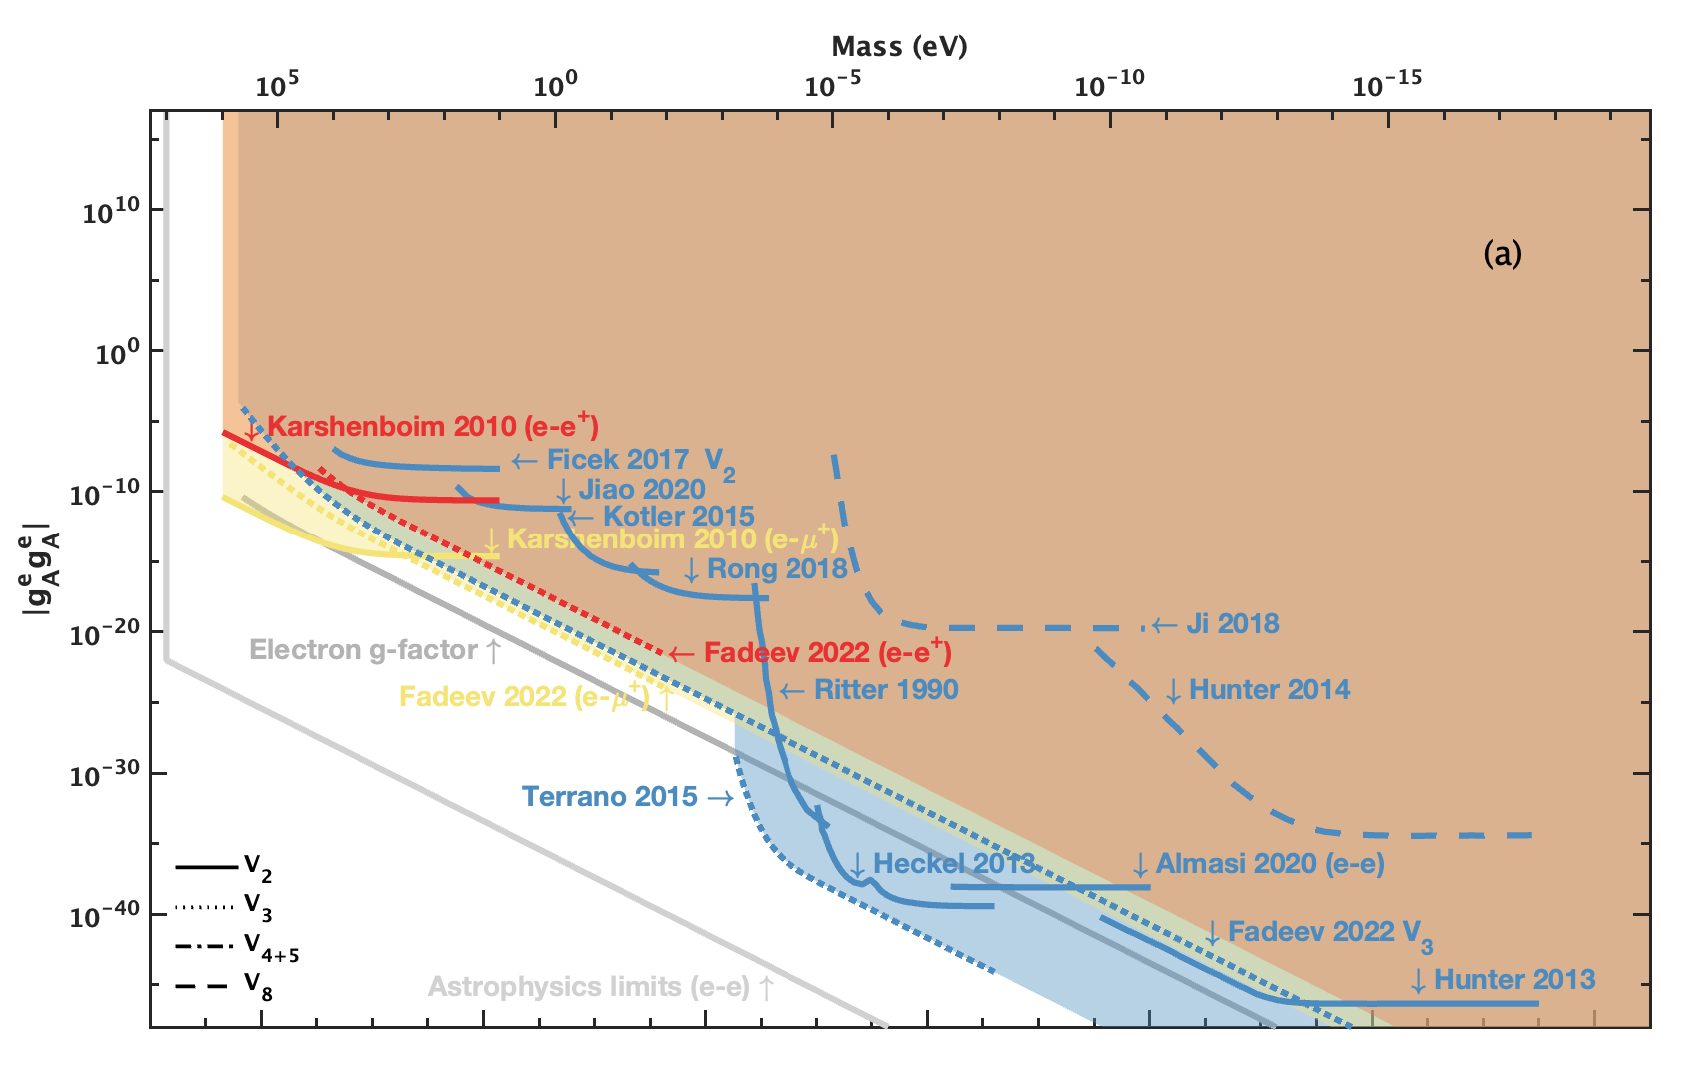
\includegraphics[width=0.88\textwidth]{Fig10_gAgA_1a.eps}

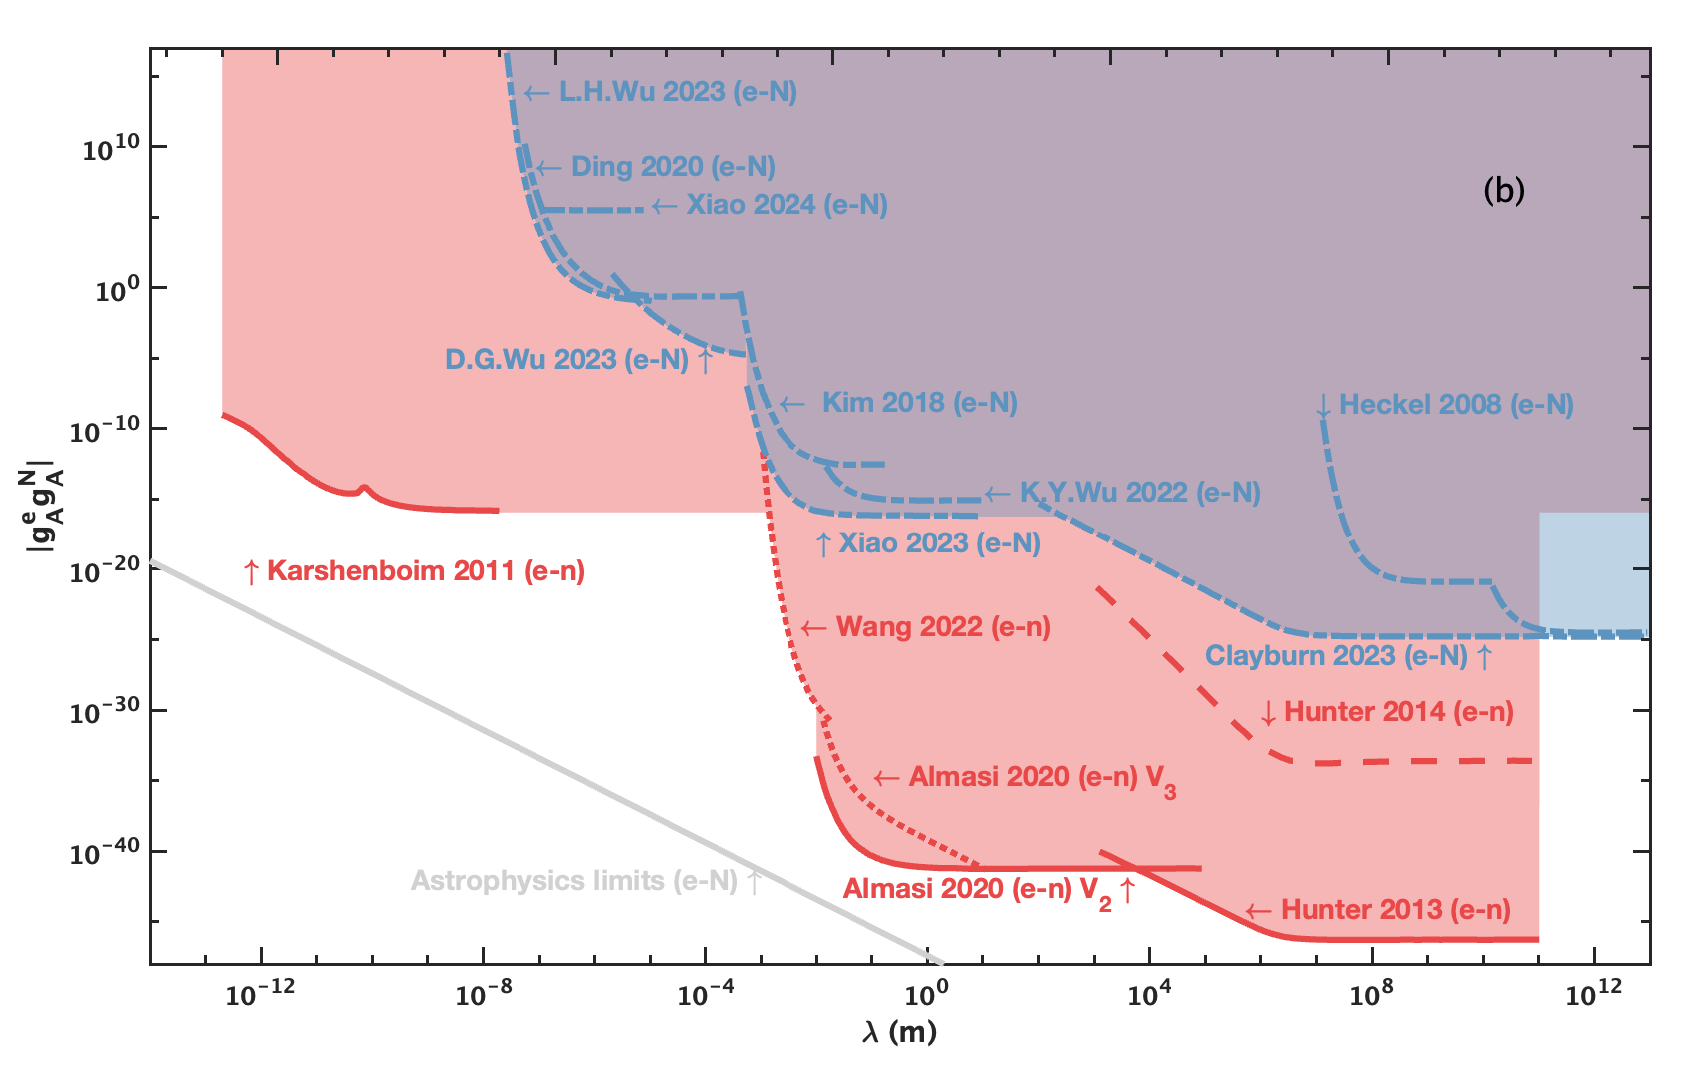
\includegraphics[width=0.88\textwidth]{Fig10_gAgA_1b.eps}
\end{center}
\caption{
%\YS{
%I still think the blue ``Fadeev 2022 $V_2$'' curve in subfigure (a) is weaker than it should be. However, I would like to raise a separate issue: As I see it, there is no simple way to obtain bounds on the $V_2$ term for $e$-$e$, $e$-$e^+$ and $e$-$\mu^+$ using only the results presented in \cite{fadeev_pseudovector_2022}, which contain contributions from both $V_2$ and $V_3$ terms in a non-trivial way. On the other hand, there are explicit bounds on the $V_2$ term presented in \cite{karshenboim_constraints_2010} for $e$-$e^+$ and $e$-$\mu^+$ and in \cite{ficek_constraints_2017} for $e$-$e$. I think it would be more transparent and simpler to present the $V_2$ bounds for $e$-$e^+$ and $e$-$\mu^+$ from \cite{karshenboim_constraints_2010}. \LC{In principle agree. Maybe ask Pasha and Filip's opinion? If this can be quickly solved, we can keep Fadeev, otherwise, we use \cite{karshenboim_constraints_2010}.}
%Indeed, we already show the bounds from \cite{ficek_constraints_2017} for $e$-$e$ in our subfigure (a) as the blue ``Ficek 2017'' curve. 
%The blue ``Ficek 2017'' curve should in principle be very similar to the blue ``Fadeev 2022 $V_2$'' curve, but they look very different. I have a couple of questions about the ``Ficek 2017'' curve as well: 
%In Figure 4 of \cite{ficek_constraints_2017}, the He-based bound on $e$-$e$ looks clearer weaker than the Ps-based bound on $e$-$e^+$, but in our subfigure (a), the two relevant curves overlap. \LC{This is my fault, we take the dotted Ps-based bound on $e$-$e^+$ from Fig.4 of \cite{ficek_constraints_2017}. I have updated it now. Now they are seperated.}The other difference evident in Figure 4 of \cite{ficek_constraints_2017} is related to the rates of fall-off of the bounds at higher boson masses: the Ps-based bounds on $e$-$e^+$ appear to transition to a mild power-law fall off, whereas the He-based bounds on $e$-$e$ appear to fall off more rapidly (potentially more similar in character to the blue ``Fadeev 2022 $V_2$'' curve, but it's not clear based on the limited mass range shown in Figure 4 of \cite{ficek_constraints_2017}). However, looking at subfigure (a), the ``Ficek 2017'' and ``Fadeev 2022 ($e$-$e^+$)'' curves both seem to fall off in the same way at higher boson masses. It would be good if we could clarify these issues.}\LC{Perhaps it is fine as we cite from the published papers.}
Constraints, depicted by coloured regions, on the coupling constant product $g_A g_A$ as a function of the interaction range $\lambda$ shown on the bottom x-axis. The top x-axis represents the new spin-1 boson mass $M$. The subscript $A$ refers to the axial-vector (pseudovector) coupling. 
%For consistency with the captions of the other results figures and to save space, I suggest the shortened rewording to replace the following part (currently commented out due to space constraints): 
Constraints are shown for \textbf{(a)} $e$-$e$, \textbf{(b)} $e$-$N$ couplings. Results are shown for $V_{2}$ (solid line), $V_{3}$ (dotted line), $V_{4+5}$ (dash-dotted line), and $V_8$ (dashed line) terms. 
Astrophysical bounds (faint, gray lines) are elaborated in Appendix~\ref{appendix_comp.}. 
%\YS{
Electron $g$-factor bounds (dark, gray line) are explained in Sec.\,\ref{METH2.g-factor}.
%} 
%\YS{Is it possible to use a darker shade of grey for the electron $g$-factor bound to more strongly differentiate it from the astrophysical bounds?} \LC{done}
Besides the depicted bounds, \citet{ficek_constraints_2017} also placed constraints on the $V_{4+5}$ and $V_8$ terms, while \citet{xiao_exotic_2024} placed constraints on $V_8$, which are not shown for clarity. 
%\YS{In subfigure (a), is it possible to adjust the position of the yellow arrow associated with the "Fadeev 2022 ($e$-$\mu^+$) $V_2$" curve so that it is closer to the associated curve? And likewise for the red arrow associated with the "Karshenboim 2011 ($e$-$n$)" curve in subfigure (b)?} \LC{done}
%\textbf{(a)} The dotted lines are the constraints from $V_{3}$ for the electron-electron ($e$-$e$) coupling which is superior to the result from $V_{2}$ (dotted lines) and $V_{8}$ (dashed lines) in general. Note that besides $V_{2}$, \textbf{Ficek 2017} also contribute other three lines from $V_{3}$, $V_{4}$, and $V_{8}$ and the latter two are the most stringent existing constraints for exotic axial-vector/axial-vector interactions $g_Ag_A$ between electrons. However, they are just a little bit above the $V_{2}$ constraint line, thus not plotted for the clarity of the figure.
%\textbf{(b)} Constraints from $V_{2}$, $V_{3}$ and $V_{8}$ for the electron-neutron ($e$-$n$) coupling (red), as well as constraints from $V_{4+5}$ and $V_{3}$ for the electron-nucleon ($e$-$N$) coupling (blue). 
%Combined bounds (faint, gray lines) are elaborated in Appendices\,\ref{appendix_comp.}. 
} 
\label{gaga-fig1}
\end{figure*}

%\LC{Comments for Fig.\,\ref{gaga-fig1}:}1. \YS{{\color{red} How were the electron-electron constraints denoted by the solid blue line ``Fadeev 2022 $V_2$'' separated from the ``Fadeev 2022 $V_3$'' bounds? The ``Fadeev 2022 $V_2$'' bound looks not as stringent as I would have expected (at the level $|g_A^e g_A^e| \sim 10^{-10}$ or so at longer ranges). }}\LC{All the three fadeev 2022 $V_2$ results are direct plot of the result Pasha sent to me. Dear Pasha, could you check this? $V_3$ bounds are transformed from $g_pg_p $ results from the paper. } 

%2. \YS{Just to confirm, where does the ``Ritter 1990'' bound on the $V_2$ term come from? In the paper \cite{ritter_experimental_1990}, they mention that their analysis presumes a dipole-dipole interaction of the form in their Eq.~(1), which looks like the $V_3$ term for the special case of a massless boson. 
%It would be helpful to clarify this in the main text.} \LC{Answered by Derek in a email.} \YS{OK}

%3. \YS{{\color{red} The astrophysical limits in both subfigures seem to be weaker (by about 18 orders of magnitude) than what I would expect based on the values in Table~\ref{tabel_Astrophysical-bounds}. Maybe the discrepancy is due to two powers of conversion between GeV and eV? It would be good to check.}} \LC{Corrected} \YS{Thank you.}

%4. \YS{\citet{almasi_new_2020} also reported a bound on $g_A^e g_A^e$. Should we add this bound to subfigure (a) and/or discuss in the main text?} \LC{yes, in the last line of Table III. We have added the line now. $r=0.25$m and $g_A^eg_A^e=8.0 \times 10^{-39}$} \YS{Thank you for adding, Lei!}

%5. \YS{\color{red} The bounds on the $V_{4+5}$ term, namely ``L.H.Wu 2023 (e-N)'', ``Ding 2020 (e-N)'' look about 8 orders of magnitude weaker than what I understand from the figures in the respective papers. Likewise, all of the other $V_{4+5}$ bounds, namely ``D.G.Wu 2023 (e-N)'', ``Kim 2018 (e-N)'', ``K.Y.Wu 2022 (e-N)'' and ``Heckel 2008 (e-N)'', also look to be similarly affected. Is there some inadvertent offset in the plotted $V_{4+5}$ bounds by chance (e.g., a numerical conversion factor like $c = 3*10^8$\,SI)?} 
%\LC{``L.H.Wu 2023 (e-N)'', ``Ding 2020 (e-N)'',``Kim 2018 (e-N)'', ``D.G.Wu 2023 (e-N)'' set constraints on $f_{4+5}^{XY}$ which have a difference $\frac{1}{4}\frac{m_X^2}{m_Y^2} \approx 3\times 10^6$. ``K.Y.Wu 2022 (e-N)'' saying under their Eq. (2) that m is the mass of the spin-polarized probing particle, which means they have use the wrong equation. To correct their result, it means a $\frac{1}{4}\frac{m_X^2}{m_Y(m_X+m_Y)} \approx 3\times 10^6$ correction is needed. \YS{Thank you for explaining, Lei! I think I understand now (up to the prefactor of 1/4 - just checking quickly, I find a prefactor of 1 for K.~Y.~Wu 2022 and a prefactor of 1/2 for the other 3 papers.)} \LCa{Yes, those factors have been taken into consideration.}
%``Heckel 2008 (e-N)'' is making a more advanced error, they have missed a factor $1/c$ in their Eq. 9. That is the reason the result in the current figure is reduced. However, we already corrected their line in our latest figure. } \YS{Thank you for checking and updating, Lei! Do you think it's worth briefly mentioning the different definitions/conventions and factor of $1/c$ in the main text?}\LCa{I plan to present them in our Github website. We can cross link to the dataset.}\YS{OK, sounds good.}


\begin{figure*} [!htbp]
\begin{center}
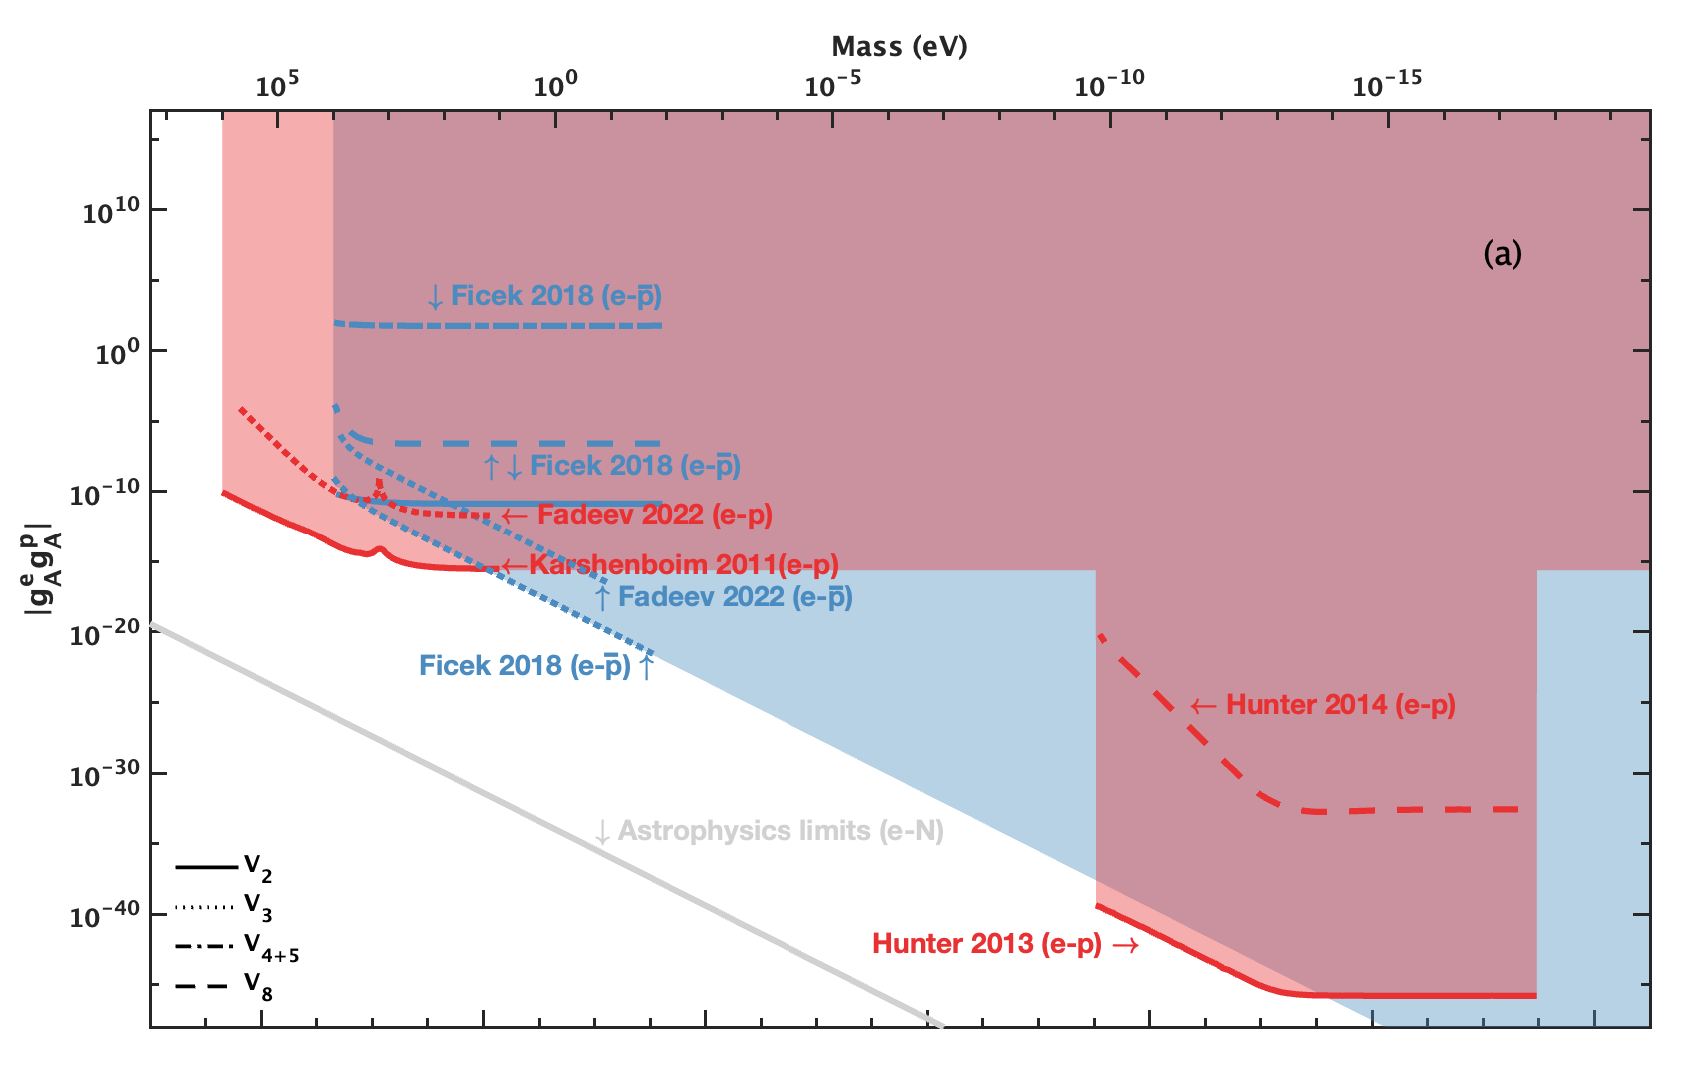
\includegraphics[width=0.88\textwidth]{Fig11_gAgA_2a.eps}

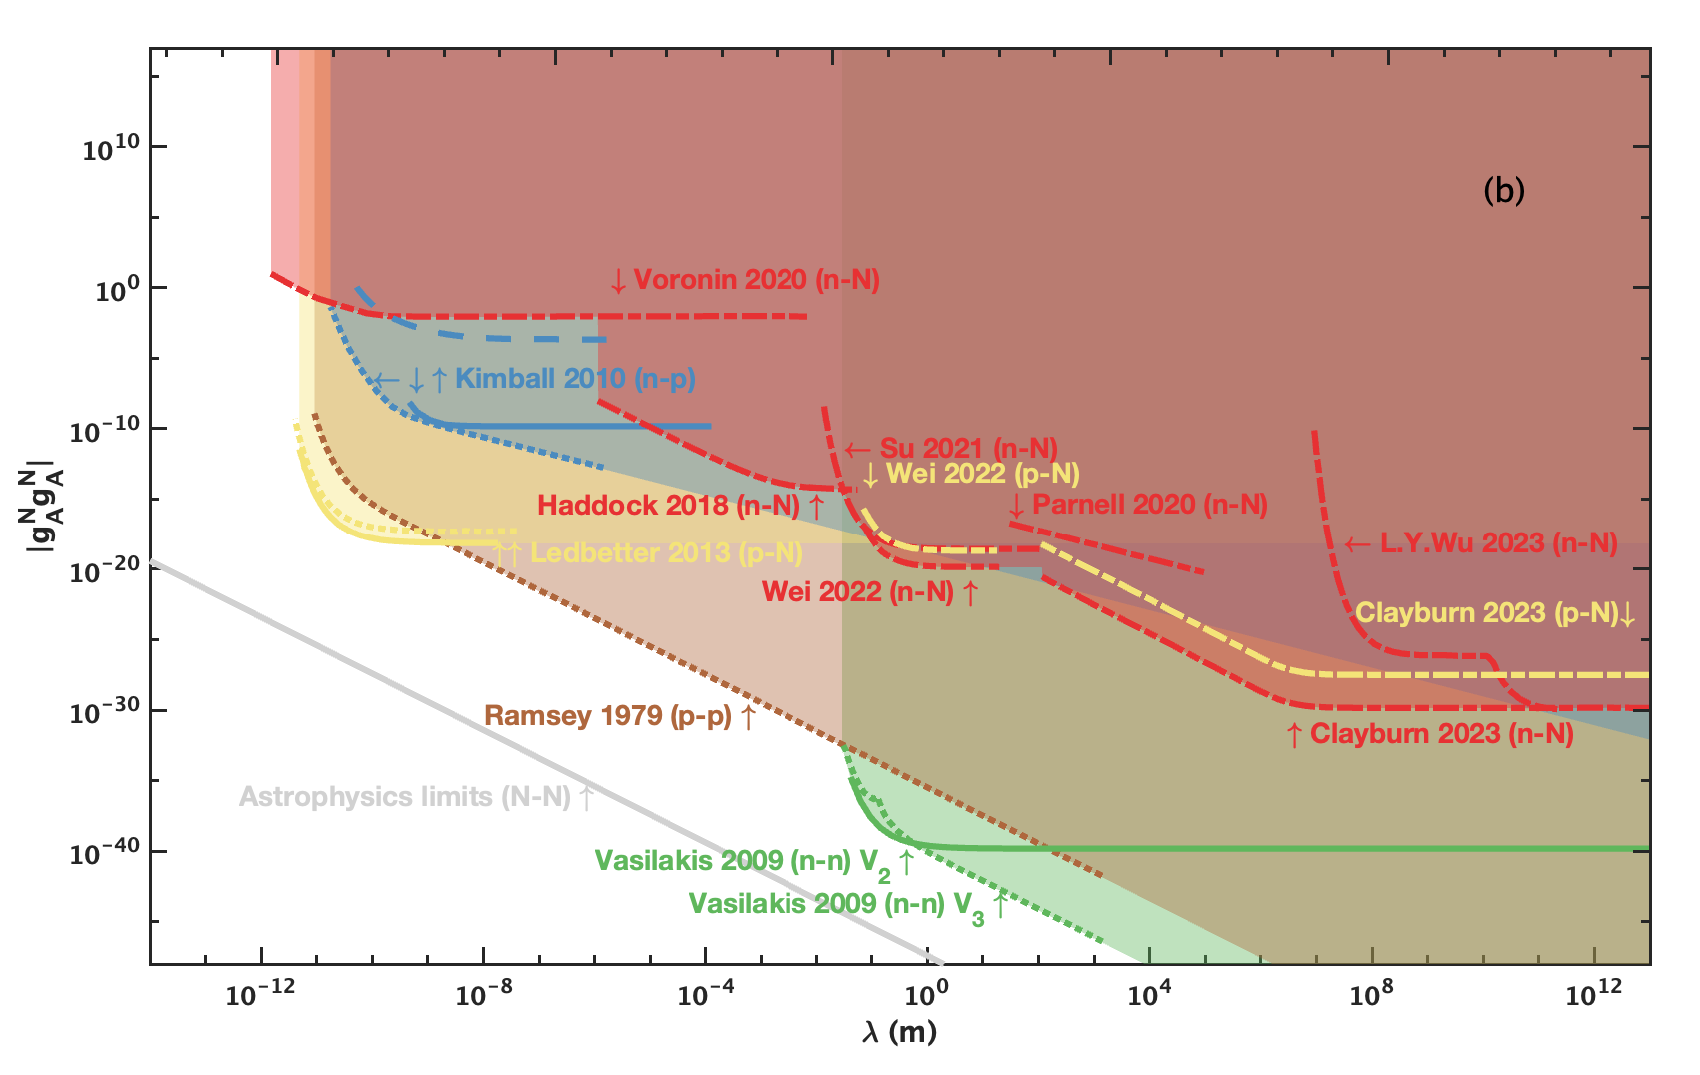
\includegraphics[width=0.88\textwidth]{Fig11_gAgA_2b.eps}
\end{center}
\caption{
%\YS{%I have a question about the $V_3$ ``Fadeev 2022 (e-p)'' red-dotted curve in subfigure (a) - why does the limit asymptote to a constant value at smaller boson masses instead of continuing to strengthen as $\propto 1/M^2$ like the other $V_3$ bounds?\LC{In Fig\,10 of Fadeev 2022, the original result for gpgp bend upward and after we add the factor $ 1/M^2$ to transfer it to gAgA, it becomes to looks flat. For other V3 constraints, they are flat at the begining and when add the factor $ 1/M^2$, they bend downward.} {\color{red}YS: Thank you for clarifying, Lei! This makes sense.} 
%In Appendix C of \cite{karshenboim_hyperfine_2011}, Savely considers a $V_3$-type short-range term, which he absorbs into a contact/delta potential, which grows like $\propto 1/M^2$ like our $V_3$ term.}\LCa{Added.}
%\LC{Yes, how about we mention this in text? There are still small differnece in coeffients, right? So, we may not be able to include their result in our figure? } {\color{red}YS: I agree that it's okay to mention this in the main text without presenting Savely's result in the figure here. (The new content in the main text looks good to me.)} \LC{Thanks, good.}
%\LCa{shaded color will be updated soon.} 
%\YS{In the top sub-figure, we currently have the y-axis label $|g_A g_A|$. Should we change this to something like $|g_A^e g_A|$ or $|g_A^e g_A^p|$ or $|g_A^e g_A^N|$?} 
Constraints, depicted by coloured regions, on the coupling constant product $g_A g_A$ as a function of the interaction range $\lambda$ shown on the bottom x-axis. 
The top x-axis represents the new spin-1 boson mass $M$. 
The subscript $A$ refers to the axial-vector (pseudovector) coupling. 
%\YS{Suggested rewording of the following part (currently commented out due to space constraints): 
Constraints are shown for \textbf{(a)} $e$-$p$, \textbf{(b)} $N$-$N$ couplings. 
Results are shown for $V_{2}$ (solid line), $V_{3}$ (dotted line), $V_{4+5}$ (dash-dotted line), and $V_8$ (dashed line) terms. 
Astrophysical bounds (faint, gray lines) are elaborated in Appendix\,\ref{appendix_comp.}.
%} 
%\textbf{(a)} Constraints from $V_{2}$ and $V_{8}$ for the electron-neutron ($e$-$p$) coupling (red), as well as constraints from all four potentials for the electron-antiproton ($e$-$\overline{p}$) coupling (blue). 
%\textbf{(b)} Constraints from all four potentials for various nucleon-nucleon ($p$-$N$, $p$-$p$, $n$-$p$ $n$-$N$ and $n$-$n$) coupling. Combined bounds (faint, gray lines) are elaborated in Appendices\,\ref{appendix_comp.}. 
}
\label{gaga-fig2}
\end{figure*}

%\LC{Comments for Fig.\,\ref{gaga-fig2}:}

%1. \YS{{\color{red} Same comment as in Fig.~\ref{gaga-fig1}: 
%The astrophysical limits in both subfigures seem to be weaker (by about 18 orders of magnitude) than what I would expect based on the values in Table~\ref{tabel_Astrophysical-bounds}. Maybe the discrepancy is due to two powers of conversion between GeV and eV? It would be good to check.}} \YS{Ok now.}

%2. \YS{The $V_{4+5}$ ``Ficek 2018 ($e$-$\bar{p}$) bound looks like it's about 8 orders of magnitude weaker than what is shown in the paper. (This looks similar to the pattern in the previous figure.) } \
%\LC{As explained before, there is a ratio between f and $g_Ag_A$. Also ``Ficek 2018" take $s=\sigma/2$ instead of the usual $s=\hbar \sigma/2$. } YS{OK, thank you for explaining!}

%3. \YS{There was also a bound on $g_A^n g_A^N$ via the $V_{4+5}$ term in \cite{piegsa_limits_2012}. Could we add the bounds to subfigure (b) and discuss in the main text?} 
%\LC{Maybe not necessary, \cite{piegsa_limits_2012} has been surpassed by \citet{haddock_search_2018} and discussed in several place in our review.} \YS{OK, fair enough.}

%4. \YS{\citet{parnell_search_2020} also constrained $g_A g_V$ via the $V_{12+13}$ term. Should we discuss those bounds in Sec.~\ref{subsec_g_Ag_V} and/or plot the bounds in Fig.~\ref{gvga-fig}?} 
%\LC{It has been surpassed by \cite{yan_searching_2015,clayburn_using_2023}, therefore we do not present it in the figure. We have mentioned about this paper.}\YS{OK}

%5. \YS{Should we add the distinguishing initials ``L.Y.'' at the front of the label ``Wu 2023 (n-N)'' to make it clearer which reference it pairs with? (Compare with Fig.~\ref{gaga-fig1}\,(b), where there are results from two other Wu 2023 papers.)} 
%\LC{Ok, done.} \YS{Thank you!}

%6. \YS{Please see my comment in Fig.~\ref{gvga-fig} and in the main text about the Vasilakis 2009 (n-n) bound.} 
%\LC{Ok, will add the line.} \YS{Thank you very much, Lei!}

%{\color{red}The key distinction between the $V_{2}$ and $V_{3}$ potentials in experimental settings is their scaling behavior with respect to particle separation $r$. The $V_{2}$ potential scales as $1/r$, whereas  $V_{3}$ scales as $1/r^3$. As a result, experiments aimed at detecting dipole-dipole interactions may exhibit significantly different sensitivities to the two potentials. }
%\YS{This isn't the complete story. The $\mathcal{V}_3$ term in the $A-A$ potential grows divergently as $\propto 1/M^2$ in the limit of small $M$, due to the non-conservation of the axial-vector current. This means that the $\mathcal{V}_3$ term can dominate over the $\mathcal{V}_2$ term for sufficiently small boson masses.}
%\LC{will make changes for above and below.}
%{\color{red}In this section, we mainly focus on the work related to $V_{2}$  because it sets the best constraints for $g_Ag_A$.} 
%\YS{This statement overlooks the presence of the $\propto 1/M^2$ enhancement for the $\mathcal{V}_3$ term in the $A-A$ potential at small boson masses. For sufficiently small $M$, $\mathcal{V}_3$ should tend to give stronger limits on the combination of parameters $g_A g_A$, due to the parametric enhancement factor $\sim 1/(Mr)^2 \gg 1$ in the limit $M \to 0$.}


%%%%
%\subsubsection{$e$-$e$, $e$-$e^+$ \&  $e$-$\mu^+$} 
%\subsubsection{\texorpdfstring{$e$-$e$, $e$-$e^+$ \& $e$-$\mu^+$}{e-e, e-e\textsuperscript{+} \& e-mu\textsuperscript{+}}}
\subsubsection{\texorpdfstring{$e$-$e$, $e$-$e^+$ \& $e$-$\mu^+$}{e-e, e-e⁺ \& e-μ⁺}}
\label{subsec_g_Ag_A_ee}
In the range $\lambda> 10^{-2}$\,m, two of the experiments \cite{hunter_using_2013,heckel_limits_2013} searching for exotic axial-vector/vector interactions discussed in Sec.\,\ref{subsec_g_Ag_V} also place strong constraints on axial-vector/axial-vector interactions between electrons, $g_A^eg_A^e$, as shown in Figure\,\ref{gaga-fig1}\,(a). In addition, \citet{almasi_new_2020} also set constraints on $g_A^e g_A^e$; see Sec.\,\ref{sec:gAgA_en} for more details of their work.

%\YS{It would be helpful to clarify somewhere in this paragraph which potential term(s) \citet{ritter_experimental_1990} actually constrained in their paper. 
%The solid blue curve ``Ritter 1990'' in Figure\,\ref{gaga-fig1}\,(a) is indicated as a bound on the $V_2$ term. 
%On the other hand, in the paper \cite{ritter_experimental_1990}, the authors mention that their analysis presumes a dipole-dipole interaction of the form in their Eq.~(1), which looks like the $V_3$ term for the special case of a massless boson. } \LCa{I think we take reference to \citet{safronova_search_2018}, Sec. VII. F. 2, [Page 55]. Derek explained this to us in a email and I added a sentence in the end of this paragraph.} 
%\YS{Thank you!} 
In the range $9\times 10^{-4} \, \textrm{m} < \lambda < 10^{-2}$\,m, \citet{ritter_experimental_1990} performed an experiment with a spin-polarized torsion pendulum made from Dy$_6$Fe$_{23}$ (see Sec.\,\ref{METH1.SOUR.ESS}) to search for feeble forces associated with a possible exotic interaction between spin-polarized masses %\YS{objects?} 
and set the most stringent limit on $g_A^e g_A^e$ until now. 
%\WJ{Shall we delete it because it is already explained before: The material used in the spin-polarized masses 
%\YS{objects?} \LCa{maybe spin-polarized masses is clear, no need to add objects?} \YS{OK}was a distinguishing feature of this experiment at that time. This is because the main practical issue in experiments looking for exotic new spin-spin interactions is that such spin-spin forces are generally expected to be much smaller than the competing magnetic dipole moment interaction between particles. However, in Dy$_6$Fe$_{23}$ compounds, which is a rare-earth and iron mixture, an \YS{intrinsic-spin/orbital?} compensation arises on a microscopic basis \YS{at a microscopic level?} \LCa{Dear Wei Ji, could you check the above two correction?} in the structure of the Dy$_6$Fe$_{23}$ material at a specific temperature (between 265\,K and 280\,K), with the magnetization due to the orbital motion of the electrons approximately cancelling the magnetization from the electron spins, allowing for the creation of a torsion pendulum with a large net intrinsic spin but a small overall magnetic moment. }
%\WJ{This is not correct and also should be deleted: This is similar to the concept behind the subsequent works in \cite{heckel_preferred-frame_2008,hoedl_improved_2011,terrano_short-range_2015}}. 
%\LC{
The constraints on the $V_2$ term for $g_Ag_A$ is based on the limit on axial photons summarized in Tab.\,VI of \citet{ritter_experimental_1990}. 
%} 
For further related discussion, see Sec.\,\ref{METH1.SOUR.ESS}. 

%For the force range $10^{-5}\,\textrm{m} < \lambda < 9\times 10^{-4}$\,m, \citet{rong_constraints_2018} established the most stringent limit on the axial-vector-mediated interaction between electron spins, using single NV centers in diamond as sensor and a single crystal of $p$-terphenyl-doped pentacene-$d_{14}$ (see Sec.\,\ref{METH1.SOUR.ESS}), placed about 12 $\mu$m away from the sensor, as the source. More details of their experiments can be found in Sec.\,\ref{METH1.SENS.SS.NV}. At $\lambda = 500\,\mu$m, their result is approximately a factor of 50 more stringent than the one set by \citet{kotler_constraints_2015} using trapped-ion measurements. 

For the force range $10^{-5}\,\textrm{m} < \lambda < 9\times 10^{-4}$\,m, \citet{rong_constraints_2018} established the most stringent limit on the axial-vector-mediated interaction between electron spins, using single NV centers in diamond as sensors and a single crystal of $p$-terphenyl-doped pentacene-$d_{14}$ (see Sec.\,\ref{METH1.SOUR.ESS}), placed about 12 $\mu$m away from the sensor, as the source. More details of their experiments can be found in Sec.\,\ref{METH1.SENS.SS.NV} At $\lambda = 500\,\mu$m, their result is approximately a factor of 50 more stringent than the one set by \citet{kotler_constraints_2015} using trapped-ion measurements.


%The polarized electrons generate an effective magnetic field on the NV electron spin through the exotic coupling,\DB{And what about also the much larger real magnetic field? How to distinguish} which results in a phase shift in the state of the sensor. This phase shift is then converted to the population of the NV-center $m_s=0$ state, which is then measured. Based on the data from three NV centers at different distances from the source, \citet{rong_constraints_2018} obtain an upper limit of the exotic dipole-dipole interaction. At 500\,\textmu m, their result is approximately a factor of 50 stricter than the one set by \citet{kotler_constraints_2015}. 


%Between $2.2\times 10^{-7}$ and $10^{-5}$ m, the best direct constraint on (axial-vector)-(axial-vector) interactions between electrons comes from the measurement of the magnetic dipole-dipole interaction between two trapped $^{88}$Sr$^+$ ions \cite{kotler_constraints_2015}. \citet{kotler_measurement_2014} trapped two $^{88}$Sr$^+$ ions using a linear radio-frequency Paul trap, and the ions were initialized in an entangled state that was insensitive to spatially homogeneous magnetic field noise. This technique enabled precise measurement of the magnetic dipole-dipole interaction between the ions, which when compared to a straightforward calculation gave good agreement at a level of $\approx 200~$ \textmu Hz. \citet{kotler_constraints_2015} then used the agreement between experiment and theory to limit the strength of exotic dipole-dipole interactions. 

In the range $2.2\times 10^{-7}\,\textrm{m} < \lambda <10^{-5}$\,m, the most stringent constraint on the axial-vector/axial-vector interaction between electrons comes from the measurement of the dipole-dipole interaction between two trapped $^{88}$Sr$^+$ ions \cite{kotler_constraints_2015}, see Sec.\,\ref{METH2.PM.TI} for more details. 
%In their earlier study \cite{kotler_measurement_2014}, two ions of $^{88}$Sr$^+$ were confined at a separation of one micrometer using a linear radio-frequency Paul trap. The ions evolved under spin-spin interactions and reached a final state that encoded information about the strength of the interaction, which could be determined by interrogating the ions. \citet{kotler_constraints_2015} compared the strength of the interaction to the theoretical calculation and the small uncertainty was translated into new constraints for the strength of axial-vector or pseudoscalar mediated interactions between electrons. 
%\citet{kotler_constraints_2015} emphasized a useful new platform for exotic particle searches benefiting from the high controllability of trapped ions and the resulting relatively straightforward analysis of systematic errors.
In addition to this, using literature data pertaining to the ground-state hyperfine splitting interval in positronium, \citet{kotler_constraints_2015} set constraints on the electron-positron axial-vector/axial-vector and pseudoscalar/pseudoscalar interactions. 
The shift in the positronium hyperfine interval caused by an exotic spin-spin interaction was estimated by using first-order perturbation theory. 
The constraints were derived from the comparison of positronium hyperfine spectroscopy data 
(\citealp{mills_new_1975}; \citealp{mills_line-shape_1983}; \citealp{ritter_precision_1984}; \citealp{ishida_new_2014})
%\cite{mills_line-shape_1983,mills_new_1975,ritter_precision_1984,ishida_new_2014} 
with QED predictions from theory \cite{eides_hard_2014}. 
Later on, the result on $g_A^e g_A^e$ has been surpassed by \citet{ficek_constraints_2017}; \citet{fadeev_pseudovector_2022} through investigation of the electronic structure of $^4$He. 
%\YS{It looks like the improved bound on $g_A^e g_A^e$ in \cite{fadeev_pseudovector_2022} came from the $V_3$ term after it was pointed out that there should be $\lambda^2$ enhancement of $V_3|_{AA}$ term, \LCa{As you may already noticed in the later text, it comes from $V_2$} \YS{{\color{red}I see now.}} whereas the results of \citet{kotler_constraints_2015} and \citet{ficek_constraints_2017} were based on the $V_2$ term. It would be good to clarify/comment on this. Should we also mention that Fig.\,\ref{gaga-fig1}\,(a) contains bounds from \cite{fadeev_pseudovector_2022} based separately on $V_2|_{AA}$ and $V_3|_{AA}$ terms?} \LCa{Yes, we can mention this here. How about: Note that the bounds on $V_2$ are extracted from the bounds on $V_{AA}(\v{r})$ presented in \citet{fadeev_pseudovector_2022}, which is a combination of $V_2|_{AA}$ and $V_3|_{AA}$ terms. Or we can direct the reader to the latter paragraph about \cite{fadeev_pseudovector_2022}.}\YS{Maybe we could use your suggested sentence and also refer the reader to the later paragraph for more details?} \LC{Ok}
%Note that the bounds on $V_2$ are extracted from the bounds on $V_{AA}(\v{r})$ presented in \citet{fadeev_pseudovector_2022}, which is a combination of $V_2|_{AA}$ and $V_3|_{AA}$ terms. 
Also, see the later paragraph that discusses \citet{fadeev_pseudovector_2022}.
Similar methods based on spectroscopy of simple atomic systems have been utilised in \citet{karshenboim_hyperfine_2011,karshenboim_constraints_2010,karshenboim_precision_2010}, see the later paragraph and Sec.\,\ref{METH2.PM.AHS} for more details. 

In the range $3.5\times 10^{-9}\,\textrm{m} < \lambda < 2.2\times 10^{-7}$\,m, \citet{jiao_searching_2020} established the most stringent constraint for an axial-vector-mediated spin-dependent interaction between electrons by using a ``molecular ruler''. 
The molecular ruler is made up of two electron spins and a shape-persistent polymer chain; the distances between spins can be tailored by varying the length of the polymer chains connecting the spins. 
The coupling strength between the two electron spins, which are separated on the nanometer scale, is determined in double electron-electron resonance (DEER) experiments. 
The detected DEER signals contain information on the possible signal of the axial-vector exotic interaction on top of the magnetic dipole-dipole interaction. Therefore, by fitting the data from five samples of varying lengths, the coupling constant $g_A^e g_A^e$ can be determined or limits placed on it. 
It is worth mentioning that \citet{jiao_searching_2020} improved on the previous limit of \citet{luo_constraints_2017} obtained from scanning tunneling microscope and electron spin resonance (STM-ESR) experiments by an order of magnitude at $\lambda=200$\,nm. 
This research \cite{jiao_searching_2020} suggests using chemically synthesized molecules to search for exotic spin-dependent interactions at the nanometer scale as a promising approach. 

In the interaction range $2.0 \times 10^{-11}\,\textrm{m} < \lambda < 3.5 \times 10^{-9}$\,m, \citet{ficek_constraints_2017} established the most stringent constraints for dipole-dipole $V_2$ interactions between electrons at the atomic scale through investigation of the electronic structure of $^4$He. 
\citet{ficek_constraints_2017} compared the spectroscopic measurements of the helium 2$^3P_1$$-$2$^3P_2$ transition 
(\citealp{castillega_precise_2000}; \citealp{zelevinsky_precision_2005}; \citealp{borbely_separated_2009}; \citealp{feng_laser-spectroscopy_2015})
%\cite{feng_laser-spectroscopy_2015, borbely_separated_2009, zelevinsky_precision_2005, castillega_precise_2000} 
and the 2$^3S_1$$-$2$^3P_{0,1,2}$ transition \cite{pastor_absolute_2004} with the theoretical calculations of the corresponding energy structure \cite{pachucki_fine_2010}. 
The difference or level of agreement between experiments and theory limits the maximal possible energy contribution that may arise from exotic interactions. 
Thereby, \citet{ficek_constraints_2017} established constraints on possible exotic interactions that may be associated with the exchange of bosonic fields. 
\citet{ficek_constraints_2017} studied the $V_{2}$, $V_{3}$, $V_{4+5}$ and $V_{8}$ potential terms. 
In Fig.\,\ref{gaga-fig1}\,(a), we present the constraints arising from the $V_{2}$ %and $V_{3}$ 
term. 
The constraints arising from the %$V_{3}$,\LC{here $V_{3}$ is the same as \citet{fadeev_pseudovector_2022}. should think about how to say. } 
$V_{4+5}$ and $V_{8}$ terms are all slightly milder than the $V_{2}$ constraint (not plotted for clarity), but these constraints are also important as they constitute the most stringent existing constraints for exotic axial-vector/axial-vector interactions between electrons. 
Is it worth mentioning that the bounds on the velocity-dependent terms $V_{4+5}$ and $V_8$ are competitive with the bound on the velocity-independent term $V_2$ in the case of helium, in contrast to typical macroscopic-scale experiments. This is because, in atoms, the typical speed of an orbiting electron is $v \sim \alpha c$, which is much larger than the relative speeds of constituent bodies in macroscopic experiments, see a related discussion of differences in speed by \citet{fadeev_revisiting_2019}. 
% \LC{Pasha, could you help with this?} \DK{This is a nice suggestion, maybe just adapt what Yevgeny wrote?}    \LC{Ok.}
As atomic theory and experiments improve, He spectroscopy is expected to become an even more sensitive probe of exotic electron-electron interactions.

In the force range $\lambda > 2.0 \times 10^{-13}$\,m, \citet{karshenboim_constraints_2010} explored the axial-vector-mediated spin-dependent interactions by comparing theory and experimental results in atomic spectroscopy and established the most stringent constraints. 
He compared the experimental and predicted values for the hfs interval $\Delta_{\text{hfs}}(1s)$ of the ground state in muonium and positronium and placed bounds on $g_A g_A$ for the fermion combinations $e$-$\mu^+$ and $e$-$e^+$, respectively. 
%\LC{Likely no need of this note:Note, \citet{karshenboim_constraints_2010} did not take the uncertainty into consideration when calculating the constraints lines. This can be done by using Eq.\,(5) from \citet{ficek_constraints_2018} and will weaken his original constraint lines for $e$-$\mu^+$ and $e$-$e^+$ by 7.6 and 1.6 times, respectively.}
\citet{karshenboim_constraints_2010} also studied hydrogen and other light hydrogenlike atoms (D, T and $^3{\rm{He}}^+$). 
\citet{karshenboim_precision_2010} used the specific difference $D_{21} = 8\Delta_{\text{hfs}}(2s) - \Delta_{\text{hfs}}(1s)$ \cite{karshenboim_hyperfine_2002-1}
%\YS{I think Savely defines the specific difference with a different overall sign; i.e., $D_{21} = 8\Delta_{\text{hfs}}(2s) - \Delta_{\text{hfs}}(1s)$} \LC{Yes, how about we cite his first paper \cite{karshenboim_hyperfine_2002-1} here? And I corrected the equation.} \YS{Thank you for updating, Lei. Yes, I like the idea to cite Savely's earlier paper here.} 
to set better constraints in a larger force range compared to the constraints based on the ground state hfs interval alone. 
A combined result of constraints from the $1s$ hfs interval and $D_{21}$ can be found in his paper \cite{karshenboim_hyperfine_2011}.

\iffalse
In the force range $5.3 \times 10^{-14}\,\textrm{m} < \lambda < 1.97 \times 10^{-11}$\,m, \citet{fadeev_pseudovector_2022} searched for axial-vector-mediated spin-dependent interactions with atomic spectroscopy and established the most stringent constraints. %\citet{fadeev_pseudovector_2022} compared experimental value for an atomic transition and SM prediction for this transition. 
%\YS{Suggested rewording:
\citet{fadeev_pseudovector_2022} compared the experimental and predicted values for atomic transitions in helium and positronium to place bounds on $g_A g_A$ for the fermion combinations $e$-$e$ and $e$-$e^+$, respectively.
\fi
%} 
%Assuming that a difference between measurement and experiment originates from an exotic spin-dependent potential, 
%considering the contribution of a spin-dependent potential to this atomic transition depends on two free parameters, boson mass and a product of coupling constants are evaluated, 
%\citet{fadeev_pseudovector_2022} obtained the constraints. 


Recently, experimental spectra of various simple atomic systems, including antiprotonic helium, muonium, positronium, helium, and hydrogen, have been reanalyzed and used to place constraints on exotic spin-dependent interactions between electrons and antiprotons ($e$-$\overline{p}$), electrons and antimuons ($e$-${\mu}^+$),
electrons and positrons ($e$-$e^+$), 
electrons and electrons ($e$-$e$), and electron and protons ($e$-${p}$) by \citet{fadeev_pseudovector_2022} following the theoretical framework in \citet{fadeev_revisiting_2019}.
% \YS{With which atomic system was this last fermion combination ($e^+$-${p}$) probed?}. \LC{corrected.}
These analyses were performed for the axial-vector/axial-vector potential $V_{AA}(\v{r})$, which receives contributions mainly from the $V_2|_{AA}$ and $V_3|_{AA}$ terms, as well as the pseudoscalar/pseudoscalar potential, for which the main contribution comes from the $V_3|_{pp}$ term, see Eq.\,\eqref{pseudoscalar-pseudoscalar_potential}. For clarity, we present the results from $V_3$. To explicitly see the effects of including both $V_2$ and $V_3$ terms, the readers are referred to the paper by \citet{fadeev_pseudovector_2022}.
%Note that \citet{fadeev_pseudovector_2022} presents compacted constraints on $g_A g_A$ from $V_{AA}(\v{r})$ which is a combination of $V_2|_{AA}$ and $V_3|_{AA}$ terms, but we easily extracted limits on $g_A g_A$ based on the $V_2|_{AA}$ term alone. %\LC{New content: \citet{karshenboim_constraints_2010} provided $e$-$e$ and $e$-$\mu^+$ constraints through $V_2$ based on the 1s hfs, and the result is almost the same as we presented. These results are not presented for clarity of the figure.}
%\YS{In Fig.\,\ref{gaga-fig1}\,(a), we have also separately extracted and presented limits on $g_A g_A$ based on the $V_3|_{AA}$ term.} \LCa{No exactly: In Fig.\,\ref{gaga-fig1}(a), we have also extracted and presented the limits on $g_A g_A$, transformed from $g_p g_p$, based on the $V_3|_{pp}$ term.}
%\YS{Thank you for explaining, Lei. Maybe we could add your sentence here? I guess that the $V_3|_{pp}$ bound in Fig.~\ref{gaga-fig2}\,(a) is obtained in a similar way?} \LC{Ok, yes.} 
In Figs.\,\ref{gaga-fig1}\,(a) and \ref{gaga-fig2}\,(a), we extracted and presented limits on $g_A g_A$, transformed from limits on $g_p g_p$, based on the $V_3|_{pp}$ term. The same approach is applied in a few other works mentioned below. Note that \citet{ficek_constraints_2017} also studied the $V_3$ term but without the $\delta$ term.



\citet{fadeev_pseudovector_2022}'s key contribution is the emphasis on the $V_3$ potential term, which is proportional to the inverse square of the mass $M$ of the mediating spin-1 boson, as discussed earlier in this Sec.\,\ref{subsec_g_Ag_A}. 
%\LCa{how about we write in the following way (I made some revision based on your comments): }\YS{OK, accepted.}
In addition, \citet{fadeev_pseudovector_2022} also emphasized that contact terms contribute to atomic spectroscopy. 
%\LC{Is the contact term in \citet{karshenboim_hyperfine_2011} the same one as ours?}
%\YS{Looking at Appendix C of \cite{karshenboim_hyperfine_2011}, it looks like his contact term is basically the same as ours, except Savely's form is applicable only for atomic $s$-wave states, whereas our form is more general and applicable to any atomic state. I think it's worth updating the text in this paragraph accordingly.} \LC{Thank you, Zhenia, I have added a sentence below.} \YS{Thank you!}
%, while they do not contribute to new forces searched for in experiments with macroscopic objects. 
%\YS{
The contribution of short-range (contact) terms in atomic-scale experiments was discussed earlier in the paper \cite{fadeev_revisiting_2019}. 
%\LC{New sentence: 
Note that a similar contact term has been studied by \citet{karshenboim_hyperfine_2011}, with the form there applicable only for atomic $s$-wave states, whereas the form by \citet{fadeev_revisiting_2019} is more general and applicable to any atomic state. 
%}
In some cases, the contact term gives the dominant or sole contribution to observable effects; for example, in the case of dipole-dipole interactions in the limit of a massless mediator, atomic $s$-wave states are only affected by the contact part of the interaction, while the contribution of the long-range part of the interaction vanishes.

%} 


%For $V_3|_{AA}$, \citet{yan_constraining_2019} used the anomalous magnetic moments and the electric dipole moments of the electron and the muon to constrain the exotic spin-dependent interactions in the range $\lambda> 8\times10^{-11}$\,m. 
%\YS{Just a general explanatory remark for here and other places where the paper \citet{yan_constraining_2019} is mentioned:} 
%The paper \citet{yan_constraining_2019} derived bounds on the electron scalar-scalar ($g_s^e g_s^e$) and pseudoscalar-pseudoscalar ($g_p^e g_p^e$) couplings using comparisons of predictions and measurements of the electron $g$-factor, as well as bounds on the muon scalar-pseudoscalar coupling ($g_s^\mu g_p^\mu$) from the experimental limit on the muon EDM. 
%Electron $g$-factor limits on $g_s^e g_s^e$ and $g_p^e g_p^e$ are also quoted in \citet{frugiuele_current_2019}. 
%Muon $g$-factor limits on $g_s^\mu$ are given in \citet{chen_muon_2017}, while a muon $g$-factor limit on $g_p^\mu$ is apparently quoted in Ref. \cite{bollig_muons_2020}.
%If the exotic particle exists, its exchange between the lepton and the antilepton would generate the anomalous lepton moments. \LC{Fig.\,\ref{yan2019-fig} shows a Feynman diagram for this process.} From the constraints on these moments one can thus obtain constraints on the exotic particles and their interactions.
\iffalse
\begin{figure} [!htbp]
\begin{center}
\includegraphics[width=0.3\textwidth]{Yan2019.png}
\end{center}
\caption{Modification of the electromagnetic vertex by exchange of a `new' boson (dashed line)
%\YS{
, which can give rise to contributions to the magnetic and/or electric dipole moment(s) of the particle.
%} 
The wavy line represents a photon and the solid line represents a lepton and antilepton. The letters indicate the four-momenta of the particles. 
Figure from \citet{yan_constraining_2019}.} \label{yan2019-fig}
\end{figure}
\fi
%\citet{yan_constraining_2019} originally reported constraints for the electron-electron (positron) pseudoscalar/pseudoscalar type interaction described by $V_{3}|_{pp}$. Since $V_{3}$ also contributes to the axial-vector/axial-vector interaction, as shown by Eq.\,\eqref{gaga_V3}, we converted their constraints for $g_p^eg_p^e$ to $g_A^eg_A^e$. More details about \citet{yan_constraining_2019} can be found in Sec.\ref{subsec_g_Pg_P}  where the results for $g_p^eg_p^e$ are discussed.
%In this work, it is assumed that if new interactions exist, they will induce anomalous magnetic moments. 
%Using the well-known Gordon decomposition formula and techniques presented by \citet{zee_quantum_2010}, \citet{yan_constraining_2019} derive the anomalous magnetic moment induced by the pseudoscalar/pseudoscalar  and pseudoscalar/scalar interaction. 
%The maximum contribution to the anomalous magnetic moment caused by exotic interaction can be determined by comparing the experimentally measured value $a_e^{exp}$ to the Standard Model (SM) prediction $a_e^{SM}$. As a result, limits for $g_A^eg_A^e$ ($g_p^eg_p^e$) can be established. Besides, exotic interactions may produce an electric dipole moment (EDM) in addition to an anomalous magnetic moment.

%\citet{yan_constraining_2019} analyzed the muon-EDM data and established constraints on the parity-violating monopole-dipole interaction mediated by ALPs. The results are presented in Sec.\,\ref{subsec_g_Pg_S}. Note that in Fig.\,\ref{gaga-fig1}, the results of \citet{yan_constraining_2019} are on the shorter-interaction-range side (heaviest new bosons); the search for even heavier bosons belongs to the high-energy physics domain \cite{butterworth_jet_2008, delannoy_probing_2013, von_buddenbrock_phenomenological_2016}.

%\citet{fadeev_pseudovector_2022} also use $V_{3}$ to set constriants for $e$-$e$ interaction, but a few orders less than \citet{yan_constraining_2019}. It is not presented in the figure for clarity.

In addition, the pseudoscalar-mediated spin-spin interaction term $V_{3}$ was used by \citet{terrano_short-range_2015} to place limits on the electron-electron coupling parameter $g_p^eg_p^e$, which has been transformed to $g_A^eg_A^e$ in our analysis. 
These limits were in the range $\lambda > 3\times 10^{-4}$\,m and are shown in Fig.\,\ref{gaga-fig1}\,(a). 
Further discussion of the experiment in \citet{terrano_short-range_2015} is given in Sec.\,\ref{subsec_g_Pg_P}. 

For the spin-spin velocity-dependent interaction term $V_8$, there are four sets of constraints on the electron-electron interaction parameter $g_A^e g_A^e$ given by 
\citet{hunter_using_2014}; \citet{ficek_constraints_2017}; \citet{ji_new_2018}; \citet{xiao_exotic_2024}.
%\cite{ji_new_2018, hunter_using_2014,xiao_exotic_2024,ficek_constraints_2017}. 
\citet{hunter_using_2014} used spin-polarized geoelectrons to search for exotic interactions in the range $\lambda>10^3$\,m as discussed in Sec.\,\ref{subsec_g_Ag_V}. 
\citet{ji_new_2018} set the stringent limits on the $V_{8}$ term based on SmCo$_{5}$ spin sources and a SERF comagnetometer in the range $5 \times 10^{-2}\,\textrm{m}<\lambda<10^3$\,m. 
%It should be noted that \citet{ji_constraints_2023} improved by an order of magnitude upon their prior limits by using two SmCo$_5$ electron-spin sources and two optically pumped magnetometers. 
%\YS{I see the earlier limits of Ji 2018 in Fig.~\ref{gaga-fig1}\,(a), but not the improved limits of \cite{ji_constraints_2023}. I also don't see the limits of \cite{xiao_exotic_2024} plotted there. Are there plans to update the figure?} \LC{seems \citet{ji_constraints_2023} study e-p interaction. Yes, \citet{xiao_exotic_2024} will be involved. }
For the range $10^{-5}\,\textrm{m}<\lambda< \times 10^{-2}$\,m, \citet{xiao_exotic_2024} elucidated the role of particle thermal motion within their theoretical model and established constraints on interactions between electrons. For a shorter interaction range, \citet{ficek_constraints_2017} set the constraints. The latter two constraint lines are not plotted for the clarity of the figure. 

%“We note that direct comparison between the electron-electron and electron-positron constraints is based on the implicit assumption of CPT invariance for the exotic interactions studied here.” \citet{kotler_constraints_2015}

%\citet{kotler_constraints_2015} electron and positron (antielectron).

%The limits for $|g_A^eg_A^{e^+}|$ of interaction between electron and positron (anti-electron) as well as the interaction between electron and anti-muon (positive muon) by potential $V_{3}$ are given by \citet{fadeev_pseudovector_2022}. 

%\citet{fadeev_pseudovector_2022} compared experimental value for an atomic transition and  Standard Model methods prediction for this transition. Assuming the difference between measurement and experiment (at 1 $\sigma$ level) originates from the exotic potential, considering the contribution of a spin-dependent potential to this atomic transition depends on two free parameters, boson mass and a product of coupling constants are evaluated,  \citet{fadeev_pseudovector_2022} obtained the constraints.  
%Existing experimental spectra of antiprotonic helium, muonium, positronium, helium, and hydrogen were analyzed to setting new limits (search for new bosons) for exotic interaction between electrons and antiprotons (e-$\overline{p}$), electrons and positrons (e-$e^+$),  electrons and antimuons (e-${\mu}^+$), electrons and electrons (e-e), and positrons and protons ($e$-${p}$),  using a potential that results from Axial-vector/Axial-vector potential (see Eq.\,\eqref{pseudovector-pseudovector_potential}) which mainly contributed by $V_{2}$ and $V_{3}$, and Pseudoscalar/Pseudoscalar potential (see Eq.\,\eqref{pseudoscalar-pseudoscalar_potential}) which mainly contributed by $V_{3}$. Note, here in Fig.\,\ref{gaga-fig1}, we also extracted the limits for $g_Ag_A$ for $V_{2}$ from the compacted $g_Ag_A$ from Eq.\,\eqref{pseudoscalar-pseudoscalar_potential}.
%In addition, \citet{fadeev_pseudovector_2022} includes contact spin-dependent terms and shows that they do contribute to atomic spectroscopy while do not contribute to new forces searched in experiments with macroscopic objects.

%%%%%
%\subsubsection{$e$-$N$}
\subsubsection{\texorpdfstring{$e$-$N$}{e-N}}
In the range $\lambda>10^{7}$\,m, \citet{heckel_preferred-frame_2008} investigated the exotic spin- and velocity-dependent interaction term $V_{4+5}$ using their torsion pendulum experiments and  established the most stringent long-range limits on the coupling parameter product $g_A^e g_A^N$, as shown in Figure\,\ref{gaga-fig1}\,(b). 
Further experimental details are discussed in Sec.\,\ref{subsec_g_Ag_V}. 

For interaction ranges around $\lambda \sim 0.1$\,m, \citet{xiao_femtotesla_2023,wu_experimental_2022,kim_experimental_2018} conducted investigations on the $V_{4+5}$ term using atomic magnetometers (see Sec.\,\ref{METH1.SENS.AM}). 
\citet{kim_experimental_2018} used a SERF magnetometer to study the $V_{4+5}$ term and established the first limits on $g_A^e g_A^N$ in this interaction range, with further details discussed in Sec.\,\ref{subsec_g_sg_s}. 
\citet{wu_experimental_2022} improved the constraints for $\lambda>2\times 10^{-2}$\,m using an atomic-magnetometer array, see Sec.\,\ref{subsec_g_Ag_V} for more details. 
%as discussed in Sec.\,\ref{subsec_g_Ag_V}. 
Recently, \citet{xiao_femtotesla_2023} further improved the constraints for $\lambda>7\times 10^{-4}$\,m by employing diffused optically polarized atoms, effectively reducing undesirable effects associated with optical pumping. 
Consequently, they established the most stringent limits on $g_A^eg_A^N$ in this range, with detailed discussions of the experiment provided in Sec.\,\ref{subsec_g_sg_s}. 


For interaction ranges around $\lambda \sim 10^{-5}$\,m, \citet{ding_constraints_2020} searched for the exotic interaction term $V_{4+5}$ by measuring the force between a gold sphere and a microfabricated magnetic structure using a cantilever (see Sec.\,\ref{METH1.SENS.MS.MMO}). 
In the range around $10^{-4}$\,m, \citet{wu_improved_2023} employed an ensemble-NV-diamond magnetometer to investigate the $V_{4+5}$ interaction and established the most stringent limits on $g_A^e g_A^N$. 
For interaction ranges on the order of $10^{-7}$\,m, \citet{wu_spin-mechanical_2023} reported the use of an on-chip detector to search for hypothetical spin- and velocity-dependent interactions, by placing a micro-scale diamond with single NV spins above a micro-mechanical resonator. 
Detailed discussion of these experiments can be found in Sec.\,\ref{subsec_g_sg_s}. 


%%%%
%\subsubsection{$e$-$n$}
\subsubsection{\texorpdfstring{$e$-$n$}{e-n}}\label{sec:gAgA_en}
In the range $\lambda> 10^{3}$\,m, \citet{hunter_using_2013} place the strongest constraints on the axial-vector/axial-vector interaction between electrons and neutrons, $g_A^e g_A^n$. 

In the interaction range $10^{-2}\,\textrm{m} < \lambda<10^{3}$\,m, \citet{almasi_new_2020} established the most stringent constraints on electron-nuclear spin-dependent forces, using a rotatable 
%\WJ{
source made with a structure of
%} 
SmCo$_5$ 
%\WJ{
covered by pure iron
%} \WJ{delete:spin source} 
[the same type as in \citeauthor{ji_searching_2017}, (\citeyear{ji_searching_2017}, \citeyear{ji_new_2018}), see Sec.\,\ref{METH1.SOUR.ESS} for more details.]  and a Rb-$^{21}$Ne comagnetometer \cite{smiciklas_new_2011}, see more details in Sec.\,\ref{METH1.SENS.AM}. 
%\WJ{This is not correct and also should be deleted: SmCo$_5$ has a unique property as a spin source: part of its magnetization is created by the orbital angular momentum of the electrons rather than their spins. This allows one to compensate the net magnetic field from the spin source  without canceling an exotic spin-dependent force}, 
%\WJ{ please delete this because it is explained in comagnetometer section:The comagnetometer (see Sec.\,\ref{METH1.SENS.AM}) is calibrated so that the external $B_z$ field \YS{Maybe worth defining/explaining what the $z$-axis is in this case?} \LCa{Dear Wei Ji, could you have a look of this?} is equal and opposite to the sum of the effective magnetic fields of polarized $^{87}$Rb and $^{21}$Ne. One can show that at this `compensation point', the device has suppressed sensitivity to ordinary magnetic fields while retaining leading order sensitivity to anomalous pseudomagnetic fields \cite{kornack_dynamics_2002,padniuk_response_2022}. The $^{87}$Rb and $^{21}$Ne atoms are contained in an aluminosilicate GE180 spherical glass-blown cell located at the heart of the comagnetometer. The cell also contains trace amounts of Cs vapor which is optically pumped to produce a relatively uniform spin polarization, which is then transferred to Rb and then to $^{21}$Ne via spin-exchange collisions. This is referred to as `hybrid optical pumping' \cite{romalis_hybrid_2010}. }
%By compensation from the external $B_z$ field, the comagnetometer has suppressed sensitivity to ordinary magnetic fields while retaining leading order sensitivity to anomalous fields. 
To convert the measured value of anomalous fields to limits on spin-spin interactions, \citet{almasi_new_2020} express the energy shift due to the exotic potentials for neutrons, protons and electrons as $\eta_n V_n  + \eta_p V_p - V_e = \mu_{^{21}\textrm{Ne}} b_y^n - \mu_\textrm{B} b^e_y$, 
%\YS{Should the RHS of this equation also contain a proton interaction parameter?}\LC{I think your question related to the definition of $b_y^{n,e}$ which are the anomalous magnetic fields that couple to the $^{21}$Ne and $^{87}$Rb electron spins in the y direction in the comagnetometer. To avoid mis-understanding, maybe we can add the above definition here?}
where $\mu_{^{21}\textrm{Ne}}$ denotes the magnetic moment of $^{21}$Ne, $\eta_n$ and $\eta_p$ 
%$\eta_n = 0.58$ and $\eta_p = 0.04$
denote the fractions of neutron and proton spin polarization in $^{21}$Ne, and $b_y^{n,e}$ are the anomalous magnetic fields that couple to the $^{21}$Ne nuclear spin and $^{87}$Rb electron spin, respectively, in the $y$ direction of the comagnetometer. 
%\YS{... that couple to the $^{21}$Ne nuclear spin and $^{87}$Rb electron spin, respectively, in the $y$ direction of the comagnetometer. ?}
%\WJ{I removed the values of eta n and eta p to avoid explaining that the values they quoted are different from what we defined.}\LC{OK}
%\YS{I have some questions about notation: Maybe we could use the notation $V_i$ instead of $\mathcal{V}_i$ for consistency with the notation of this review and the notation in \cite{almasi_new_2020}? Likewise, maybe we could use the notation $\eta_{n,p}$ instead of $f_{n,p}$ for consistency with the rest of the review? To me, the original notation $\mu_{^{21}\textrm{Ne}}$ used in \cite{almasi_new_2020} is clearer than $\mu_{21}$. Or if $\mu_{^{21}\textrm{Ne}}$ is too clunky, then maybe we could use something like $\mu_\textrm{Ne}$ instead?} 
%\LCa{done}
%They took into account $f_{n/p}$, the fraction of neutron and proton spin polarization in $^{21}$Ne, and 
%\WJ{Delete this: \citet{almasi_new_2020} integrate the exotic potential term $V_2$ (or $V_3$) over the distribution of the polarized spins in the SmCo$_5$ magnets and the soft-iron flux return, and obtain limits separately on pseudoscalar and axial-vector coupling constants, the latter of which} \WJ{Their results on $V_3$} are shown in Fig.\,\ref{gaga-fig1}\,(a,\,b). 
\citet{almasi_new_2020} studied the exotic potential term $V_2$ ($V_3$) between $e$-$e$ and $e$-$n$, the results are shown in Fig.\,\ref{gaga-fig1}\,(a,\,b).
 
%\LC{as $V_n f_n +V_p f_p -\sV_e=\mu_{^{21}Ne}b_y^n-\mu_B b^e_y$ where $f_{n/p}$ is the fraction of neutron/proton spin polarization in $^{21}$Ne, and $b^{n/e}_y$ are the anomalous magnetic fields that couple to the $^{21}$Ne and $^{87}$Rb electron spins in the $y$ direction. And the interaction is given by Eqs.\,\ref{gaga_V2} and \ref{gaga_V3}, and are integrated over the distribution of the polarized spins in the SmCo$_5$ magnets and the soft-iron flux return.

In the range $2 \times 10^{-13}\,\textrm{m} < \lambda < 10^{-2}$\,m, \citet{karshenboim_hyperfine_2011} set the most stringent constraints on spin-dependent interactions mediated by axial-vector light bosons. 
\citet{karshenboim_hyperfine_2011,karshenboim_constraints_2010,karshenboim_precision_2010} compared spectroscopic measurements of hyperfine structure intervals to quantum electrodynamics calculations (see Sec.\,\ref{METH2.PM.AHS}) for various atomic systems in order to derive constraints on axial-vector interactions. 
%In contrast to his earlier work, \citet{karshenboim_hyperfine_2011} used a updated experimental data and 
%used a specific difference  of the hyperfine structure intervals in the $1s$ and $2s$ states, $D_{21} = 8 E_\textrm{hfs}(2s) - E_\textrm{hfs}(1s)$, that is only sensitive to the $V_2$ term, in order to disentangle the $V_2$ term from a contact term, which arises in the spin-spin interaction alongside the $V_2$ term. 
Previous constraints on spin-spin interactions were derived from data pertaining to the hyperfine structure interval of the $1s$ state in light hydrogenlike atoms \cite{karshenboim_constraints_2010}, where the accuracy was constrained either by the hyperfine structure internal measurements or by the uncertainty in the related contribution of nuclear effects. 
The theory of the 
%\YS{
specific difference of the $1s$ and $2s$ hyperfine intervals, $D_{21} = 8 E_\textrm{hfs}(2s) - E_\textrm{hfs}(1s)$ 
\cite{karshenboim_precision_2010,karshenboim_hyperfine_2011}, however, is practically insensitive to short-range contributions (including nuclear effects and associated uncertainties).
%}. 
%however, is comparatively impervious to issues with calculating magnetic moments and other fundamental constants.
Due to the cancellation of the nuclear contributions, which have significant uncertainties, the theory of the difference becomes more accurate in the case when $\lambda$ is larger than atomic distances. 
In hydrogen, deuterium and the $^3$He$^+$ ion, this makes it possible to constrain the product of coupling constants, $g_A^e g_A^N$, for the spin-spin electron-nucleon interaction at a level below one part in $10^{16}$ in the sub-keV boson mass region ($\lambda > 2\times 10^{-10}$\,m). 
For super-keV boson masses, the constraints derived in \citet{karshenboim_precision_2010,karshenboim_hyperfine_2011} from data pertaining to the $D_{21}$ %{\color{red}$1s$ hfs interval} \YS{Shouldn't this be the specific difference $D_{21}$ here? Please check.} \LC{Yes, corrected.}
become weak and must be combined with the findings of \citet{karshenboim_constraints_2010}, which considered the $1s$ hyperfine structure interval. 
%Although the constraints in \citet{karshenboim_constraints_2010} are milder in the keV mass range and at smaller masses, they are better suited for extension to higher masses such as the MeV range ($\lambda \approx 2\times 10^{-13}$\,m). 
%As a result, the constraints on exotic spin-spin interactions at the shortest scales have been set by \citet{karshenboim_constraints_2010}.
In Figs.\,\ref{gaga-fig1}\,(b) and \ref{gaga-fig2}\,(a), we present the combined constraints from \citet{karshenboim_hyperfine_2011}.  
Note that \citet{karshenboim_hyperfine_2011} studied (in his App.\,C) a $V_3$-type short-range term, which contains a contact delta potential and grows like $\propto 1/M^2$ at small boson masses, similar to our $V_3|_{AA}$ term. 

Besides the $V_2$ term, there are a few other sets of constraints on exotic interactions between $e$-$n$ that have been derived from experiments via the $V_3|_{AA}$ and $V_8$ terms. 
%\YS{What about the $V_{4+5}$ term?} 
In the case of the exotic dipole-dipole potential $V_3|_{AA}$, in the range $2 \times 10^{-2} \, \textrm{m} < \lambda < 10$\,m, \citet{almasi_new_2020} set the most stringent constraints on the coupling parameter product $g_A^eg_A^n$; 
in the interaction range $4 \times 10^{-4} \, \textrm{m} < \lambda < 2 \times 10^{-2}$\,m, \citet{wang_limits_2022} set the most stringent constraints on $g_A^e g_A^n$, which is described in more detail in Sec.\,\ref{subsec_g_Pg_P}. 
For the velocity-dependent exotic spin-spin potential term $V_8$, \citet{hunter_using_2014} used geoelectrons, which were discussed in Sec.\,\ref{subsec_g_Ag_V}, to set the only bounds thus far on $g_A^e g_A^n$. 





%%%%
%\subsubsection{$e$-$p$ \& $e$-$\overline{p}$}
\subsubsection{\texorpdfstring{$e$-$p$ \& $e$-$\overline{p}$}{e-p \& e-p̅}}
For the exotic axial-vector/axial-vector interaction between the fermion pair $e$-$p$, there are four sets of limits, as shown in Fig.\,\ref{gaga-fig2}(a). 
Two of these sets are for long interaction ranges and were derived by using geoelectrons to probe the potential terms $V_2$ \cite{hunter_using_2013} and $V_8$ \cite{hunter_using_2014} that we discuss in Sec.\,\ref{subsec_g_Ag_V}. 

The other two sets of constraints are for shorter interaction ranges and were obtained by comparing spectroscopic measurements of hyperfine splitting intervals to quantum electrodynamics calculations 
%{\color{red}for various atomic systems} \YS{``
in atomic hydrogen
%''? --- which other atomic systems, besides atomic hydrogen, are sensitive to $e$-$p$ without being sensitive to $e$-$n$?} 
using the $V_2$ \cite{karshenboim_hyperfine_2011} 
%(\citealp{karshenboim_hyperfine_2011}; \citealp{fadeev_pseudovector_2022})
%\cite{karshenboim_hyperfine_2011,fadeev_pseudovector_2022}
and $V_3$ \cite{fadeev_pseudovector_2022} terms. 
For more details on Karshenboim's work and \citet{fadeev_pseudovector_2022}, see Sec.\,\ref{subsec_g_Ag_A_ee}. 
\iffalse While utilizing the same data for the $1s$ and $2s$ hyperfine transitions in hydrogen for the specific difference of the $1s$ and $2s$ hyperfine intervals, $D_{21} = 8 E_\textrm{hfs}(2s) - E_\textrm{hfs}(1s)$, \citet{karshenboim_hyperfine_2011} and \citet{fadeev_pseudovector_2022} 
%originally \YS{What do we mean by ``originally'' here? Does this mean at longer interaction ranges?} \LCa{We updated \citet{fadeev_pseudovector_2022}'s result only and presented the updated result in the figure. I'm thinking we can indicate it as "This work". However, we are a review paper, not sure we need to do this. We are also considering to publish it seperately, but the result is not significant enough yet. Perhaps we publish it with some other results.}\YS{I see. In this case, if we present the updated/reinterpretted bound based on \citet{fadeev_pseudovector_2022}, then we should clearly state/explain this.} 
provide almost the same constraints using the $V_2$ term. 
\fi
%The discrepancy at shorter ranges arises from the use of different expressions; specifically, \citet{karshenboim_hyperfine_2011} incorporates a profile function, while the latter does not. 
%The discrepancy arises from that \citet{karshenboim_hyperfine_2011} incorporates the constraints from 1s hfs results which gives better constraints at shorter ranges \cite{karshenboim_precision_2010,karshenboim_constraints_2010}. 
Note that improved constraints from hydrogen based on the analysis of the $D_{21}$ interval \cite{karshenboim_precision_2010} and the latest experimental results \cite{bullis_ramsey_2023} and theory \cite{yerokhin_electron_2008} are presented by \citet{cong_improved_2024}. 

\iffalse
In Fig.\,\ref{gaga-fig2}(a), we present an improved result based on the method of \citet{fadeev_pseudovector_2022} and the latest experimental results from \cite{bullis_ramsey_2023}. 
The experimental results used in \citet{fadeev_pseudovector_2022} were $D_{21}=48.923(54)$ kHz,
%\YS{For which interval(s)? Or is this for the specific difference $D_{21}$?}
and the corresponding theoretical result was $D_{21}= 48.953(3)$ kHz
%\YS{For which interval(s)? Or is this for the specific difference $D_{21}$?}, 
leading to $\Delta E = 0.102$\,kHz (at a 90\% confidence level). 
The new experimental result of 48.9592(68) kHz from \citet{bullis_ramsey_2023}, coupled with the theoretical prediction of 48.9541(23) kHz %\YS{Why do we use this particular theory value here instead of the value quoted in the previous sentence? In principle, the theory value in \cite{yerokhin_electron_2008} was known at the time of both \cite{karshenboim_hyperfine_2011} and \cite{fadeev_pseudovector_2022}. (Why) Was it not used in those papers?} \LC{They didn't use it. They both use some ealier theoretical result around 2005 and 2006.}\YS{OK, this makes sense.}
from \cite{yerokhin_electron_2008}, yield $\Delta E = 0.0144$\,kHz. 
This represents a sevenfold improvement over the original constraints established by \citet{fadeev_pseudovector_2022}. 
\YS{Who set these constraints? (Is there a separate reference for this?) And what do we mean by ``original constraints'' in this context? Were the constraints in \cite{fadeev_pseudovector_2022} updated? Or are we just deriving a new set of constraints ourselves here and plotting these constraints in Fig.\,\ref{gaga-fig2}(a) under the label ``Fadeev 2022 (e-p)''? If so, then I think the description in this paragraph is confusing and inconsistent with our approach in the rest of the review --- in this case, my suggestion would be to plot the bounds of \cite{fadeev_pseudovector_2022} in Fig.\,\ref{gaga-fig2}(a) as-is and mention/describe in the text that it is possible to improve on the bounds of \cite{karshenboim_hyperfine_2011} and \cite{fadeev_pseudovector_2022} by a factor of about 7 using the new experimental result for $D_{21}$ from \cite{bullis_ramsey_2023}.} \LC{Yes, now we decide to put on arXiv our notes and then cite them here. Will update here soon.}
\YS{OK}
\DK{Good!}
\fi

%THE OLD VERSION
%For the exotic interaction between fermions pair e-$\overline{p}$, \citet{ficek_constraints_2018-1} compare theoretical calculations and spectroscopic measurements of the hfs of antiprotonic helium to set the most stringent constraints on $\sV_2$, $\sV_3$, $\sV_{4+5}$ and $\sV_8$. xxx

For the exotic semi-leptonic e-$\overline{p}$ interaction, \citet{ficek_constraints_2018} compared theoretical calculations and spectroscopic measurements of hyperfine splitting intervals in antiprotonic helium ($^4$He$^+$$\bar{p}$) 
%the hfs of antiprotonic helium 
to set constraints on the $V_2$, $V_3$, $V_{4+5}$ and $V_8$ terms. 
They focused on antiprotonic helium with the antiproton in the $(n,l) = (37,35)$ state and the electron in the $(n,l)=(1,0)$ state. 
Here $n$ and $l$ denote the principal and orbital quantum numbers, respectively. 
The transition energies between the relevant hyperfine-structure states were measured experimentally by \citet{pask_antiproton_2009} and theoretically calculated by \citet{korobov_calculation_2008}. 
Comparison of these values gives $\Delta E = 0.3(1.3)$\,MHz (e.g. $\Delta E = 2.2$\,MHz at 90\%\,C.L.), which leads to the constraints presented in Fig.\,\ref{gaga-fig2}\,(a). 


%\LC{need to add \citet{ji_constraints_2023} line and text.}
%In addition, the only limits for $|g_Ag_A|$ of interaction between positron (antielectron) and antiproton ($e^+$-$\overline{p}$) by potential $\sV_{3}$ is \citet{fadeev_pseudovector_2022} which has just been discussed. \LC{seems it is $e$-$\overline{p}$ (Top panel of Fig.\,1 in \citet{fadeev_pseudovector_2022}) and has been surpassed by \citet{ficek_constraints_2018} of $\sV_{3}$ for a few orders. Thus the line will not be presented. }


%%%%
%\subsubsection{$N$-$N$}
\subsubsection{\texorpdfstring{$N$-$N$}{N-N}}
\label{subsec_g_Ag_A:N-N}
In this section, we present limits on $g_A g_A$ for interaction between nucleons, including the combinations neutron-nucleon ($n$-$N$), proton-neutron ($p$-$N$), proton-proton ($p$-$p$), neutron-proton ($n$-$p$) and neutron-neutron ($n$-$n$), as shown from left to right in Fig.\,\ref{gaga-fig2}\,(b). 
%\YS{What do we mean by ``from left to right'' here? Does this mean in terms of the order in which the combinations appear? If we ignore the astrophysical bounds on $N$-$N$, then the leftmost set of bounds is for $n$-$N$.} 
Although many results are presented here, some of them, such as the results based on the $V_{3}$ term are discussed in detail in Sec.\,\ref{subsec_g_Pg_P}, while those pertaining to the $V_{4+5}$ term are discussed in Sec.\,\ref{subsec_g_sg_s}. 
Below, we introduce each limit individually. 


%%%
%\paragraph{$p$-$N$ interactions} 
\paragraph{\texorpdfstring{$p$-$N$ interactions}{p-N interactions}}
For the interaction range $6.5 \times 10^{-12}\,\textrm{m} < \lambda <  2.0 \times 10^{-8}$\,m (i.e., around the atomic scale), \citet{ledbetter_constraints_2013} derive constraints on the existence of the exotic spin-spin Yukawa potential term $V_2$ (as well as the dipole-dipole potential term $V_3$) and set the most stringent limits. 
The constraints are derived by comparing NMR measurements (\citealp{neronov_nmr_1975}; \citealp{beckett_temperature_1979}; \citealp{gorshkov_determination_1989}; \citealp{helgaker_nmr_2012})
%\cite{helgaker_nmr_2012,gorshkov_determination_1989,beckett_notitle_1979,neronov_nmr_1975} 
with theoretical calculations 
(\citealp{oddershede_nuclear_1988}; \citealp{vahtras_indirect_1992}; \citealp{enevoldsen_correlated_1998}; \citealp{helgaker_nmr_2012})
%\cite{helgaker_nmr_2012,enevoldsen_correlated_1998,vahtras_indirect_1992,oddershede_nuclear_1988} 
of the $J$-coupling parameter in deuterated molecular hydrogen (HD), see Sec.\,\ref{METH2.PM.NMR} for more details. 
%Such $J$ couplings coupling between the magnetic moments of the two hydrogen nuclei and have the form $J\,\boldsymbol{I}\cdot\boldsymbol{S}$ (here, $\boldsymbol{I}$ and $\boldsymbol{S}$ are the respective spins of the proton and deuteron, respectively).
%The difference in $\Delta\,J$ between theory and experiment is regarded as an upper bound on the magnitude of an exotic spin coupling. 
%Note that, for consistency with the per-nucleon normalisation in our Eq.\,\eqref{ANZ}, the constraints from this work, which involved the combination $g_A^2 = g_A^p + g_A^n$, need to be divided by a factor of 2; i.e., $g_A^N = g_A^2/2$ in the case of deuteron. 
%\YS{
Note that for consistency with the per-nucleon normalisation in our Eq.\,\eqref{ANZ}, the constraints from \citet{ledbetter_constraints_2013}, which involved the combination $g_A^N = g_A^p + g_A^n$, are translated here to constraints on the combination $g_A^N = (g_A^p + g_A^n)/2$ in the case of deuteron.\footnote{We remark that the case of deuteron, which has two unpaired nucleon spins (one proton and one neutron), is special. Most non-deformed nuclei with nonzero spin have only one unpaired nucleon spin, in which case $g_A^N = g_A^{n,p}$ is already normalised correctly per-nucleon without the need for an extra factor of $1/2$.}
%} 
%\YS{Is it worth adding this example to the paragraph after Eq.\,\eqref{ANZ}? (Or is better to avoid mixing discussion of axial-vector couplings with vector couplings?)} \LCa{This is something quite specific. Maybe we just mention it here. } \YS{OK}
The constraints derived in this study outperform previous laboratory limits that were derived from studies of spin-exchange collisions between $^3$He and Na atoms \cite{jackson_kimball_constraints_2010}. See also the recent constraints based on $J$-coupling in tritium deuteride (DT) \cite{cong_constraints_2024}. 
\citet{ledbetter_constraints_2013} also suggest that spin systems with a small $J$-coupling may help to significantly improve these limits.
%\DKIns{
Chemically unbound systems, such as liquid $^3$He-H$_2$ mixtures \cite{hiza_liquid-vapor_1981}, can have nonzero $J$-coupling due to second-order hyperfine effects when the constituent species form van der Waals molecules. The $J$-coupling in these systems can be orders of magnitude smaller than that in HD. For relatively simple systems, the theoretical value of the $J$-coupling may be able to be calculated with an accuracy approaching that for HD. This combination of factors could significantly reduce the absolute uncertainty in the determination of anomalous energy shifts, and consequently improve sensitivity to exotic spin-dependent interactions.
%}
%\DKDel{The advantage of such systems is that a lower relative accuracy is required for calculating the $J$-coupling parameters to obtain a given level of sensitivity to exotic interactions.} \YS{Is this due to the simple electronic structures of the species involved? Maybe worth briefly clarifying the specific reason(s) for this here.} \LC{Dear Derek, could you please kindly take a look of this?} \DK{I tried to explain a bit more above, what do you think?}\LC{Ok. What do you think, Zhenia?}\YS{Dear Derek and Lei, thank you for clarifying and updating this part! I like this reworded explanation.} 

Additionally, in the range $\lambda > 0.1$\,m, \citet{wei_constraints_2022} established a limit on $g_A^pg_A^N$ for the exotic potential term $V_{4+5}$ using a K-Rb-$^{21}$Ne comagnetometer, see Sec.\,\ref{subsec_g_sg_s} for more details. 

%And their result is superier than the limit for $g_A^pg_A^N$ for the exotic potential $\sV_{4+5}$ set by \citet{parnell_search_2020}

%\paragraph{$p$-$p$ interactions}
\paragraph{\texorpdfstring{$p$-$p$ interactions}{p-p interactions}}%\LC{new content, need read: 
For the range $\lambda >10^{-11}$\,m,
%\YS{Fig.\,\ref{gaga-fig2}\,(b) appears to show the constraints for $\lambda > 10^{-11}$\,m. Is the range quoted here correct? The Ramsey papers appears to use the figure of merit $\lambda = 10^{-13}$\,cm}
\citet{ramsey_tensor_1979} constrained the $V_3$ term based on spectroscopy
%nuclear spectra \YS{Were these specifically nuclear spectroscopy experiments? (If not, then maybe can just use the generic term ``spectroscopy experiments''?)} 
experiments with the hydrogen molecule (H$_2$). 
By comparing the measurements of \cite{harrick_nuclear_1953} to theoretical calculations of the magnetic dipole-dipole interaction between the protons in H$_2$, \citet{ramsey_tensor_1979} set the only constraint on the exotic interaction between protons. 
Note that we have taken the limit presented in Fig.\,16 of Ref.\,\citet{safronova_search_2018} and convert this into a bound on $V_3|_{AA}$. 
%\YS{Fig.~16 of \citet{safronova_search_2018} shows bounds for the pseudoscalar $V_3|_{pp}$ term. For clarity, maybe we could explain that we take this bound as input and convert this into a bound on $V_3|_{AA}$? On a related note, is there a particular reason why we use Fig.~16 of \citet{safronova_search_2018} for the input bounds on $V_3|_{pp}$ instead of, e.g., Fig.~1 from the earlier paper \cite{ledbetter_constraints_2013}?} \LC{No special reason, just we find it first in \citet{safronova_search_2018}}


%%%%
%paragraph{$n$-$p$ interactions}
\paragraph{\texorpdfstring{$n$-$p$ interactions}{n-p interactions}} In the interaction range $\lambda > 3.7 \times 10^{-10}$\,m, \citet{jackson_kimball_constraints_2010} compared experimental measurements (\citealp{soboll_spin_1972}; \citealp{borel_spin-exchange_2003})
%\cite{borel_spin-exchange_2003,soboll_spin_1972}
and theoretical estimates (\citealp{walker_estimates_1989}; \citealp{tscherbul_collision-induced_2009})
%\cite{tscherbul_collision-induced_2009,walker_estimates_1989} 
of spin-exchange cross sections between Na and $^3$He atoms to constrain exotic spin-dependent forces. 
For the Na-$^3$He collisions, the interaction of colliding atoms is dominated by the spin-independent interatomic potential while spin exchange is dominated by a much smaller, spin-dependent potential arising from penetration of the Na valence electron wavefunction inside the $^3$He nucleus \cite{walker_spin-exchange_1997}.
%\YS{Do we mean nuclei or core electrons (or both)?}. \LCa{I think it is nuclei. Dear Derek, could you please check?}
%If the usual spin-dependent potentials arising from electromagnetic interactions are augmented with exotic spin-dependent potentials generated by the exchange of new force-mediating particles, 
One can calculate the contribution of exotic spin-dependent potentials generated by the exchange of new-force-mediating particles to the spin-exchange cross sections and thus constrain the range and coupling strengths of such hypothetical particles from the agreement between experiment and conventional theory. 
The work of \citet{jackson_kimball_constraints_2010} established limits on the previously unconstrained exotic spin-spin Yukawa-type $V_2$ potential term between neutrons and protons. 
In addition, the dipole-dipole potential term $V_3$ in the range $2.0 \times 10^{-11}\,\textrm{m} < \lambda < 2.0 \times 10^{-6}$\,m and the velocity- and spin-dependent interaction term $V_8$ in the range $\lambda > 4.9 \times 10^{-11}$\,m were also constrained. 


%%%%
%\paragraph{$n$-$N$ interactions}
\paragraph{\texorpdfstring{$n$-$N$ interactions}{n-N interactions}} In the range $\lambda>10^{-12}$\,m, \citet{haddock_search_2018}; \citet{voronin_constraint_2020}; \citet{parnell_search_2020}; \citet{su_search_2021}; \citet{wei_constraints_2022}; \citet{wu_new_2023}
%\citet{voronin_constraint_2020,haddock_search_2018,su_search_2021,wei_constraints_2022,parnell_search_2020,wu_new_2023} 
collectively set the most stringent constraints via the potential term $V_{4+5}$, see Sec.\,\ref{subsec_g_Ag_V} for more details on \citet{su_search_2021} and Sec.\,\ref{subsec_g_sg_s} for details of the other experiments. 
%\YS{What about discussion of the bounds ``Voronin 2020 (n-N)'' at shorter ranges and ``Wu 2023 (n-N)'' at longer ranges? Could we add some (brief) discussion here about these bounds from Fig.\,\ref{gaga-fig2}\,(b), possibly with cross-references to other section(s) where they are discussed (perhaps in more detail)?} \LC{maybe we direct the reader to Sec.\,\ref{subsec_g_sg_s} directly.}



%In the range between $10^{-2} <\lambda< 10^{5}$, \citet{su_search_2021} and \citet{parnell_search_2020} set the most stringent constraints for $g_A^ng_A^N$ on the spin- and velocity-dependent interaction $\sV_{4+5}$. The former has been introduced in Sec.\,\ref{subsec_g_Ag_V} and the latter will be discussed in Sec.\,\ref{subsec_g_sg_s}.



%%%%
%\paragraph{$n$-$n$ interactions} 
\paragraph{\texorpdfstring{$n$-$n$ interactions}{n-n interactions}}
For interaction ranges around $\lambda \sim 10$\,m, \citet{vasilakis_limits_2009} has set the most stringent constraints on the dipole-dipole interaction term $V_3|_{pp}$. 
In addition, this work also provided constraints on couplings to light vector bosons, including bounds on $g_A g_A$ via the $V_2$ term and bounds on $g_A g_V$ via the $V_{11}$ term. 
%As indicated by the arrow in the bottom-right corner of Fig.\,\ref{gaga-fig2}\,(b), the bounds on $g_A g_A$ via the $V_2$ term from this experiment are $1.5 \times 10^{-40}$ for the special case of a massless spin-1 boson. 
Further details about this experiment can be found in Sec.\,\ref{subsec_g_Pg_P}. 

%\LC{some newly added experimental results need text, such as $\sV_{4+5}$ Longhao Wu with quantum chip, and \cite{wu_improved_2023,xiao_femtotesla_2023,wu_new_2023}. }


%\LC{\citet{fadeev_pseudovector_2022} missing some lines?}


%%%%
\subsubsection{Future perspectives} 

There are many intriguing possibilities for probing exotic interaction mediated by new spin-1 axial-vector bosons in the future. 

For the $V_{2}$ term, \citet{chen_optomechanical_2020}; \citet{wang_proposal_2023}; \citet{guo_searching_2024}
%\citet{chen_optomechanical_2020,wang_proposal_2023,guo_searching_2024} 
propose novel experimental methods.
\citet{chen_optomechanical_2020} introduce a spin-resonator hybrid mechanical system, where an NV center is magnetically coupled to a cantilever resonator, and the probe absorption spectrum can be used to measure the exotic dipole-dipole interaction. 
\citet{wang_proposal_2023} propose a novel force sensor based on a cantilever to measure the exotic interactions in a periodic stripe magnetic source structure and a closed-loop magnetic structure integrated with the cantilever. 
The sensitivity to $g_A^e g_A^e$ in the interaction range $3 \times 10^{-8} \, \textrm{m} < \lambda < 10^{-3}$\,m is expected to be better than the sensitivities demonstrated in 
\citet{kotler_constraints_2015}; \citet{rong_constraints_2018}; \citet{jiao_searching_2020}.
%\citet{rong_constraints_2018,kotler_constraints_2015, jiao_searching_2020}. 
%\citet{wang_proposal_2023} can also design different periodic magnetic structures for $V_3$, which allows performing joint data analysis under the assumption that both $V_2$ and $V_3$ could exist. 
\citet{guo_searching_2024} proposed to use a diamond-based vector magnetometer with ensembles of nitrogen-vacancy centers along different axes to search for exotic spin-spin interactions between electrons and nucleons. The constraints via $V_2$ can be improved in the interaction range 
%\YS{Maybe $10^{-8}$\,m or even $10^{-9}$\,m for the lower mass bound?} \LC{Ok.}
$\sim 10^{-8} \, \textrm{m} < \lambda < 10^{-2}$\,m. 

Considering the significant impact of the $V_3$ term on the overall landscape of constraints realised in recent years, the NMR experiments proposed in \citet{arvanitaki_resonantly_2014}, which may establish unprecedented sensitivity to $g_A^e g_A^N$ and $g_A^N g_A^N$ for interaction ranges around $\lambda \sim 10^{-2}$\,m, appear particularly promising. 
More details about this proposed experiment can be found in Sec.\,\ref{gpgs_emerging}. 
%\LC{New content: 
In addition, \citet{guo_searching_2024} may also improve the constraints for $e$-$N$ via $V_3$
%\DKDel{(one needs to transfer the constraints for $V_3|_{pp}$ to $V_3|_{AA}$)} \DK{I think that side note is not necessary in this context.} \LC{Ok, thanks.}
within the interaction range $ 10^{-8} \,\textrm{m} < \lambda < 10^{-4}$\,m.
%} 
%\YS{Do \citet{guo_searching_2024} explicitly mention that they will probe the axial-vector/axial-vector coupling via the $V_3$ term? It looks like they focus on the $V_2$ term for the axial-vector/axial-vector case, while the $V_3$ term is discussed for the pseudoscalar-pseudoscalar case. It also looks more like a proposal/projections rather than actual constraints have been obtained.} \LC{Yes, their paper is a prosal. We can transfer their constraints for $V_{pp}$ to  $V_{AA}$.}


%\YS{There's also a new proposal to use a diamond-based vector magnetometer with ensembles of nitrogen-vacancy centers along different axes in a diamond to probe $g_A^e g_A^N$ and $g_p^e g_p^N$, described in \url{https://arxiv.org/abs/2402.15042}.} 



%%%%%%%%%%%%%%%%%%%%%%%%%%%%%%%%%%%%%%%%%%%%%%%%%%%%%%
                      % R3. g_Vg_V
%%%%%%%%%%%%%%%%%%%%%%%%%%%%%%%%%%%%%%%%%%%%%%%%%%%%%%

%\subsection{Vector/Vector interaction $g_Vg_V$ }
\subsection{\texorpdfstring{Vector/Vector interaction $g_Vg_V$}{Vector/Vector interaction gVgV}}
\label{subsec_g_Vg_V}

Experimental constraints on the exotic vector/vector combination of parameters $g_V g_V$ come from the potential terms $V_1$, $V_{2}+V_{3}$ and $V_{4+5}$: 
%$V_{3}$ and $V_{4+5}$:

%\YS{In principle, we could omit the factors of $\hbar$ and $c$ in the equations below like we do in Eq.~(\ref{vector-vector_potential}) above by setting $\hbar = c = 1$. \LC{Just to make sure it is more clear to experimental physicists and make all the results easier to compare, I prefer to add $\hbar$ and $c$ everywhere. People make mistakes about this sometimes.} \LC{disc. 5} We can simply copy and paste the relevant terms from Eq.~(\ref{vector-vector_potential}) and tidy up the expressions by combining multiplicative pre-factors and remove the underbraces from the expressions.
%I would propose to first present the potential terms $\mathcal{V}_1$, $\mathcal{V}_{2+3}$ and $\mathcal{V}_{4+5}$, then point out below that (most) prior analyses in the literature have considered $\mathcal{V}_3$ instead of $\mathcal{V}_{2+3}$ - at that point, we can present the relevant equation for $\mathcal{V}_3$ - and explain the effect on exclusion plots along the lines in the orange text below. \LC{Thanks, will present as suggested.} 
%(As an aside, the equation for $\mathcal{V}_2+\mathcal{V}_3$ below appears to have a stray erroneous part marked in red. Please check.\LC{It may not be a mistake. To make gg dimensionless, we need to add this coefficient. It is not presented in Eq.~(\ref{vector-vector_potential} because you set $\hbar = c = 1$. We can add  $\hbar$ and $c$ back. } {\color{green}YS: It may not necessarily be incorrect, but the inclusion of factors of $\hbar$ and $c$ only for this term and not the others doesn't look consistent; e.g., there's another $\mathcal{O}(\lambda^2 r)^{-1}$ term in Eq.~(\ref{gVgV_V23}) that doesn't have a similar prefactor before it.} ) The equation for $\mathcal{V}_{4+5}$ should match the relevant term in Eq.~(\ref{vector-vector_potential}) using anticommutators - need Pasha to first double-check this.\LC{will check this later.}} 


%\begin{equation}
%\label{vector-vector_potential}
%V_{VV}(\v{r}) = g^X_V g^Y_V \underbrace{ \frac{e^{-M r}}{4 \pi r} }_{\mathcal{V}_1}
%+  \frac{g^X_V g^Y_V }{4} \underbrace{ \left[ \v{\sigma}_X \cdot \v{\sigma }_Y  \left[ \frac{1}{r^3} + \frac{M}{r^2} + \frac{M^2}{r} - \frac{8 \pi}{3} \delta(\v{r}) \right]  -  \left( \v{\sigma}_X \cdot \hat{\v{r}} \right) \left( \v{\sigma }_Y \cdot \hat{\v{r}} \right)  \left[ \frac{3}{r^3} + \frac{3M}{r^2} + \frac{M^2}{r} \right]  \right] \frac{e^{-M r}}{4 \pi m_X m_Y} }_{\mathcal{V}_2 + \mathcal{V}_3} \, ,
%\end{equation}

\begin{equation}
\label{gVgV_V1}
V_1|_{VV} = g^X_V g^Y_V \frac{\hbar c}{4\pi}\frac{e^{-{r}/{\lambda}}}{r} \, , 
\end{equation}

\begin{widetext}
\begin{equation}
\label{gVgV_V23}
(V_2+V_3)|_{VV} = g_V^Xg_V^Y\frac{\hbar^3}{16\pi c m_Xm_Y}\left[ \v{\sigma}_X \cdot \v\sigma_Y^{\,\prime} \left[ \frac{1}{r^3} + \frac{1}{\lambda r^2} + \frac{1}{\lambda^2 r} - \frac{8 \pi}{3} \delta(\v{r}) \right]  -  \left( \v{\sigma}_X \cdot \hat{\v{r}} \right) \left( \v\sigma_Y^{\,\prime}\cdot \hat{\v{r}} \right)  \left( \frac{3}{r^3} + \frac{3}{\lambda r^2} + \frac{1}{\lambda^2 r} \right)  \right] e^{-{r}/{\lambda}} \, , 
\end{equation}
%\begin{equation}\label{gVgV_V45}
%begin{aligned}
%V_{4+5}=g_V^Xg_V^Y \frac{\hbar^2}{16\pi c}\frac{2m_X+m_Y}{m_X(m_X+m_Y)}\boldsymbol{\sigma}_X \cdot(\boldsymbol{v} \times \hat{\boldsymbol{r}}) \left(\frac{1}{r^2}+\frac{1}{\lambda r}\right) e^{-\frac{r}{\lambda}}\,,
%\end{aligned}
%\end{equation}
%The modified $V_{4+5}|_{VV}$ will be, obtained similar to Eq.\,\eqref{gaga_V45}.
\begin{equation}
\label{gvgv_V45new}
\begin{aligned}
V_{4+5}|_{VV}&=\frac{g_V^X g_V^Y}{4} \frac{\hbar^2}{c} \left\{ \boldsymbol{\sigma}_X \cdot \left( \frac{\boldsymbol{p}_X}{m_X^2} \times \hat{\boldsymbol{r}} \right) 
 - 2 \boldsymbol{\sigma}_X \cdot \left( \frac{\boldsymbol{p}_Y}{m_X m_Y} \times \hat{\boldsymbol{r}} \right)
, \left( \frac{1}{r^2} + \frac{1}{\lambda r} \right) \frac{e^{-{r}/{\lambda}}}{8 \pi} \right\} \\
%&=\frac{g_V^X g_V^Y}{4} \boldsymbol{\sigma}_X \cdot \left( \frac{1}{m_X^2} \frac{m_X m_Y (\boldsymbol{v}_X-\boldsymbol{v}_Y)}{m_X+m_Y}- 2  \frac{1}{m_X m_Y} \frac{m_X m_Y (\boldsymbol{v}_Y-\boldsymbol{v}_X)}{m_X+m_Y}\right) \times \hat{\boldsymbol{r}} \left( \frac{1}{r^2} + \frac{M}{r} \right) \frac{e^{-Mr}}{4 \pi}  \\
 &\Rightarrow g_V^X g_V^Y \frac{\hbar^2}{16\pi c}\frac{2m_X+m_Y}{m_X(m_X+m_Y)}\boldsymbol{\sigma}_X \cdot(\boldsymbol{v} \times \hat{\boldsymbol{r}}) \left(\frac{1}{r^2}+\frac{1}{\lambda r}\right) e^{-{r}/{\lambda}} \, , 
\end{aligned}
\end{equation}
\end{widetext}
with the second line of $V_{4+5}|_{VV}$ [Eq.\,\eqref{gvgv_V45new}] expressed in a commonly used form for macroscopic experiments. 
%taken the two-body C.M. framework into consideration. %, i.e. $\boldsymbol{p}_X=m_X \frac{m_Y (\boldsymbol{v}_X-\boldsymbol{v}_Y)}{m_X+m_Y}$ and $\boldsymbol{p}_Y=m_Y \frac{m_X (\boldsymbol{v}_Y-\boldsymbol{v}_X)}{m_X+m_Y}$, and for simplify, $\boldsymbol{v}=\boldsymbol{v}_X-\boldsymbol{v}_Y$.



%It is noticed 
We note that, similarly to the axial-vector/axial-vector case in Sec.\,\ref{subsec_g_Ag_A}, the potential associated with the vector/vector interaction also includes contributions from the $V_3$ and $V_{4+5}$ terms; however, there are key differences between the two cases. 
In the axial-vector case, the $V_3|_{AA}$ term diverges as $\propto \lambda^2$ as $\lambda$ increases -- there is no such divergence for the closely related $(V_2+V_3)|_{VV}$ term in the vector case. 
In the axial-vector case, $V_{4\pm5}|_{AA}$ only has spin-momentum correlations of the type $\boldsymbol{\sigma}_X \cdot \boldsymbol{p}_Y$ and $\v\sigma_Y^{\,\prime} \cdot \boldsymbol{p}_X$, whereas in the vector case, $V_{4\pm5}|_{VV}$ has additional correlations of the type $\boldsymbol{\sigma}_X \cdot \boldsymbol{p}_X$ and $\v\sigma_Y^{\,\prime} \cdot \boldsymbol{p}_Y$. 
See Sec.\,\ref{Subsec:Fformalism} for more and related discussion. 


Prior analyses in the literature for the vector case have considered the sole term $V_3$ (defined in the equation below) instead of the combined term $V_2+V_3$: 
%, see $V_3$ below: 
%\YS{I think the sign of the delta function term (marked in red) in the equation below should be reversed to a plus sign. Please check.} 
\begin{widetext}
\begin{equation}
\label{gVgV_V3}
\begin{aligned}
V_{3}|_{VV}=g_V^Xg_V^Y\frac{\hbar^3}{16\pi c m_Xm_Y}\left[ \v{\sigma}_X \cdot \v\sigma_Y^{\,\prime} \left[ \frac{1}{r^3} + \frac{1}{\lambda r^2}  + \frac{4 \pi}{3} \delta(\v{r}) \right]  -  \left( \v{\sigma}_X \cdot \hat{\v{r}} \right) \left( \v\sigma_Y^{\,\prime}\cdot \hat{\v{r}} \right)  \left( \frac{3}{r^3} + \frac{3}{\lambda r^2} + \frac{1}{\lambda^2 r} \right)  \right] e^{-{r}/{\lambda}} \, . 
\end{aligned}
\end{equation}
\end{widetext}
The difference between the $V_3$ limits reported in the literature and the (correct) $V_2+V_3$ limits that are appropriate for $g_Vg_V$ is relatively small on a logarithmic scale. Therefore, while future analyses should be done with the $V_2+V_3$ combination noted in Sec.\,\ref{Subsec:Fformalism} and in \citet{fadeev_revisiting_2019}, here in this review we choose to keep the $V_3$ bounds from earlier literature. 
%From a technical point of view: 
For $Mr \ll 1$, when $\exp(-Mr) \approx 1$ and the constraints on $g_V g_V$ are generally at their strongest and are approximately independent of $M$, the typical relative difference between bounds on $V_{3}|_{VV}$ and $(V_2 + V_3)|_{VV}$ is $\mathcal{O}(Mr)^2 \ll 1$.
%\YS{Please check this statement} {\color{red}$\mathcal{O}(Mr) \gg 1$} \YS{$\mathcal{O}(Mr)^2 \ll 1$}.\LCa{Dear Wei ji, could you please check this?} \DK{I believe that Yevgeny is correct here that the difference between the potentials scales as $\mathcal{O}(Mr)^2 \ll 1$.}\LC{Ok, many thanks!}
For $Mr \gg 1$, when the exponential character of the function $\exp(-Mr)$ dominates over the power-law terms, the relative difference in the shapes of exponential tails of limit curves for $V_{3}|_{VV}$ and $(V_2+V_3)|_{VV}$ is generally larger (but still small on the log-log scale). 


%\LCa{Still need to check the literature to see if any related contents should be included. I think most of them about $f_{\perp}$.}

Figure~\ref{gVgV-fig} shows the current laboratory constraints on $g_V^X g_V^Y$ between the studied particle pairs (a) $e$-$e$, $e$-$e^+$ and $e$-$\mu^+$, (b) $e$-$N$, $e$-$n$, $e$-$p$ and $e$-$\overline{p}$, and (c) $n$-$N$, $p$-$N$, $p$-$p$, $n$-$p$ and $n$-$n$. 
Constraints from the spin-independent $V_1$ term and astrophysical bounds are also presented for comparison, see Sec.\,\ref{METH2.Astro.} and Appendices\,\ref{appendix_V1} and \ref{appendix_comp.} for more details. 

%The horizontal axes at the bottom show the range of interaction $\lambda$, inversely proportional to the mass $M$ of the boson (top axis) mediating the interaction, $\lambda=\hbar/(Mc)$. The vertical axes show the dimensionless coupling parameter $|g_Vg_V|$. 
%\YS{I propose to also add astrophysical bounds and spin-independent $\mathcal{V}_1$ laboratory bounds here. \LC{Yes, will add.}
%For the $\mathcal{V}_1$ laboratory bounds, we can simply transfer all of the $\mathcal{V}_1$ limits for the scalar-scalar case in Fig.\,\ref{gsgs-fig} (after adding them there), since the expressions for the $\mathcal{V}_1$ potential terms in the scalar and vector cases only differ by an overall sign, so there's no difference when presenting bounds on the modulus of coupling parameters $|g_s g_s|$. 


\begin{figure} [!htbp]
\begin{center}
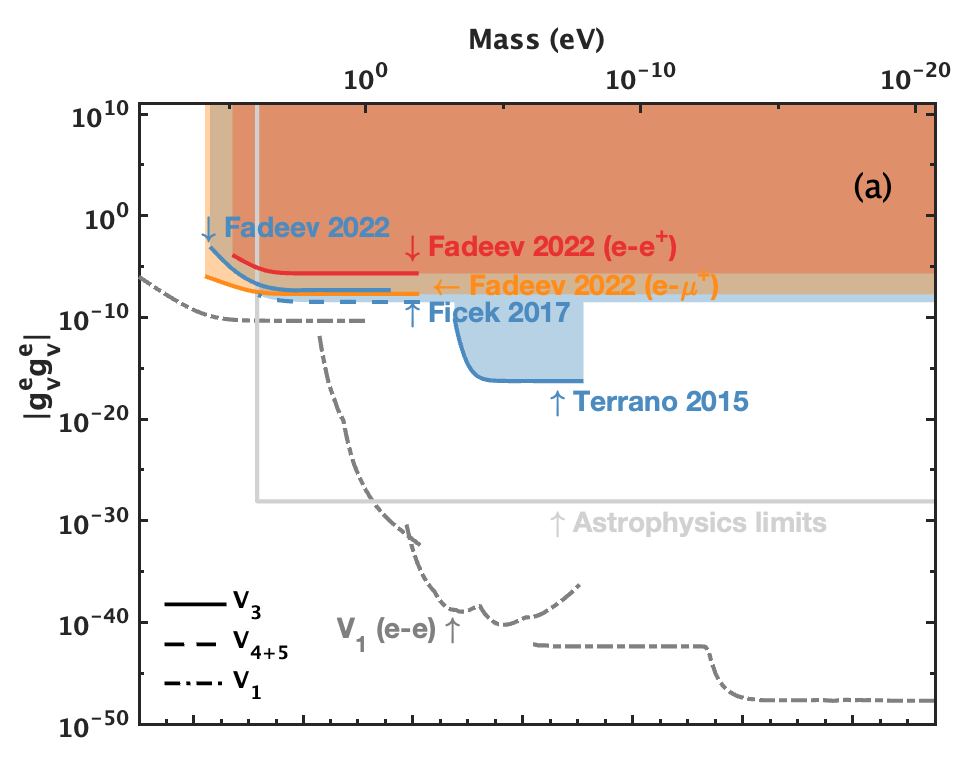
\includegraphics[width=0.48\textwidth]{Fig12_gVgV_a.eps}

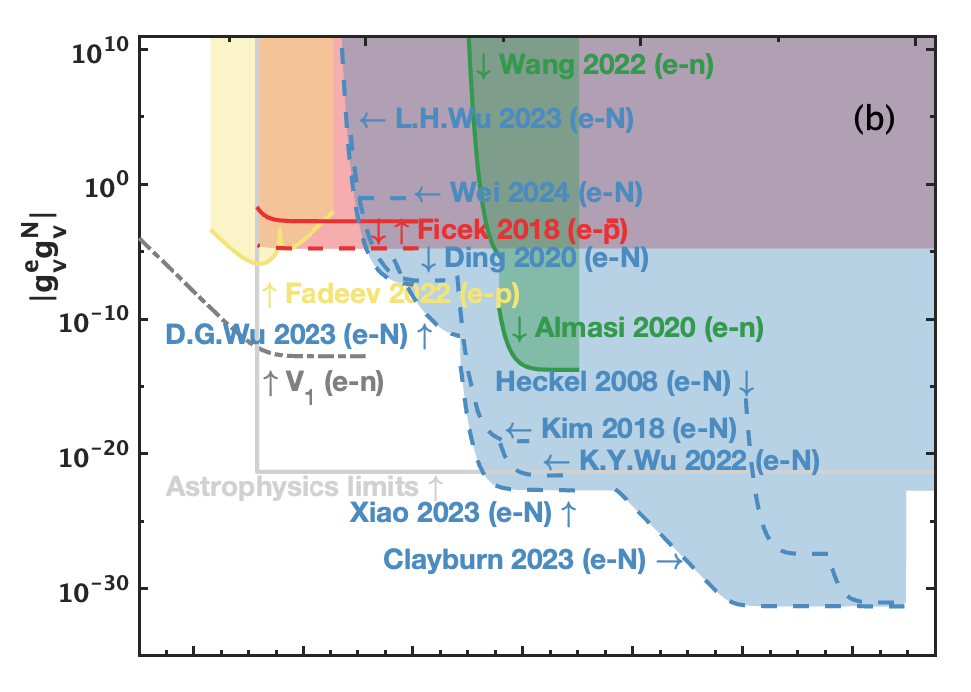
\includegraphics[width=0.48\textwidth]{Fig12_gVgV_b.eps}

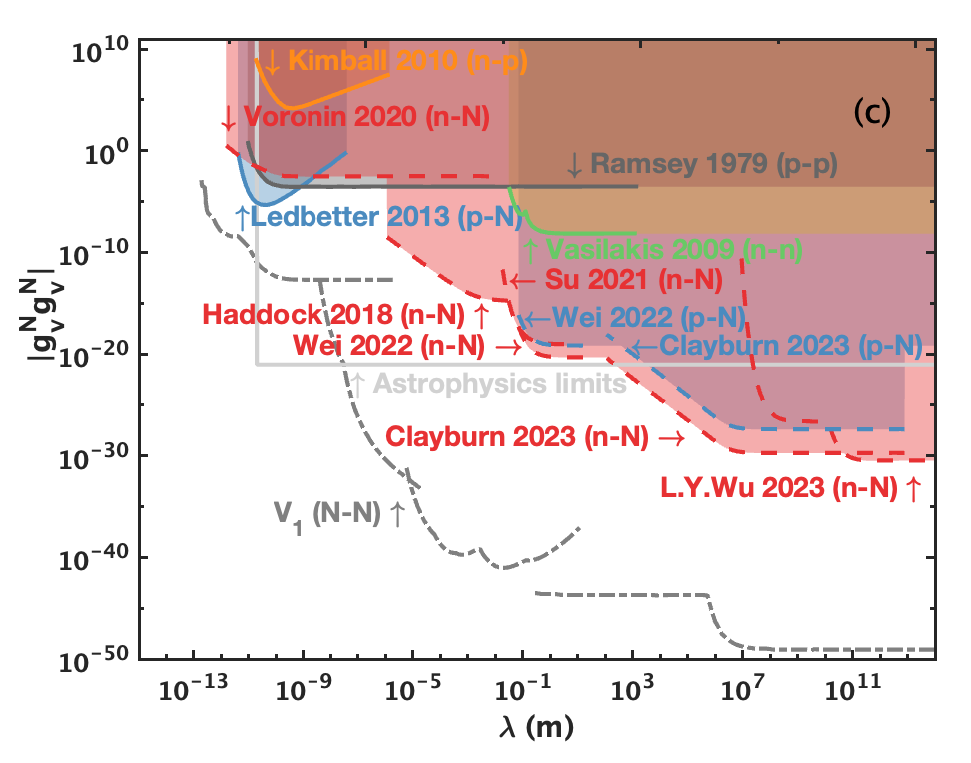
\includegraphics[width=0.48\textwidth]{Fig12_gVgV_c.eps}
\end{center}
\caption{
%\YS{In subfigure (a), it looks the "Fadeev 2022 ($e$-$e^+$)" bound comes from the 1S-2S interval in positronium. Why don't we use the stronger (by a factor of about 9) bound from the ground-state hyperfine interval in positronium here?} \LC{Yes, will update to the data from Figure 7 in Fadeev 2022.}\YS{Thank you, Lei!}\LC{done}
%\YS{Is it possible to adjust the positions of the arrows associated with the "Ficek 2017" curve in subfigure (a), "Fadeev 2022 (e-p)" curve in (b), and "Ledbetter 2013 (p-N)" curve in (c) to be closer to their respective curves?}\LC{Done.} 
%\YS{{\color{red}Figure temporarily made in two-column format to make room for comments below. Please change back to single-column format when needed.}} 
Constraints, depicted by coloured regions, on the coupling constant product $g_A g_A$ as a function of the interaction range $\lambda$ shown on the bottom x-axis. 
The top x-axis represents the new spin-1 boson mass $M$. 
% shown on the bottom x-axis. 
%(a) Constraints from $V_{3}$ and $V_{4+5}$ for the $e$-$e$ coupling (blue), constraints from $V_{3}$ for the $e$-${\muon}^+$ coupling (green) and $e$-$e^+$ coupling (red). 
The subscript $V$ refers to the vector coupling. 
Constraints are shown for \textbf{(a)} $e$-$e$ (blue), $e$-${\mu}^+$ (green), $e$-$e^+$ (red); 
\textbf{(b)} $e$-$N$ (blue), $e$-$n$ (green), $e$-$p$ (yellow), $e$-$\overline{p}$ (red); 
\textbf{(c)} $n$-$N$, $p$-$N$, $p$-$p$, $n$-$p$ and $n$-$n$ (various colors). 
%\YS{
Results are shown for $V_3$ (solid line) and $V_{4+5}$ (dashed line) terms.
%} 
%\YS{
Additional bounds from the spin-independent $V_1$ term (dash-dotted, dark grey line) and astrophysics (solid, light grey line) are elaborated in Appendices\,\ref{appendix_V1} and \ref{appendix_comp.}.
%} 
%Additional constraints for comparison, from $V_1$ and astrophysics, are explained in App.\,\ref{appendix_V1} and \ref{appendix_comp.}. 
} 
\label{gVgV-fig}
\end{figure}

%{\color{red}Comments for Fig.\,\ref{gVgV-fig}:} 
%1. \YS{{\color{red} The ``$V_1$ (e-e)'' (and possibly also ``$V_1$ (e-n)'') curves containing $g_V^e$ may need to be updated. Please see the discussion around Eq.~(\ref{gse-alpha}).}} 
%\LC{ $V_1$ (e-e) has been updated. $V_1$ (e-n) we take directly the result from ``Delaunay 2017" presented in $|g_sg_s|$ in appendix. Is this ok? If so ,we do not need to update.} \YS{Thank you for updating, Lei! Yes, I think the Delaunay 2017 (e-n) bound was already correct.}
 

%2. \YS{In subfigure (a), maybe can position the label ``Ficek 2017'' on the bottom-side of the dashed curve with the arrow pointing up (in order to provide more space between it and the ``Fadeev 2022'' curve)?} \LC{Ok}

%3. \YS{The astrophysics limits on $|g_V^e g_V^N|$ in subfigure (b) look a bit stronger than what I would expect based on the values in Table~\ref{tabel_Astrophysical-bounds}. I would expect something like $g_V^e g_V^N \leq [(g_V^e)^2+(g_V^N)^2]/2 \sim 10^{-21}$. Please check.} \LC{corrected} \YS{Thank you for checking and updating, Lei!}

%4. \YS{The digit ``4'' in $10^{14}$ on the bottommost x-axis appears to be cut off on the righthand side - is it possible to restore it?} \LC{done} \YS{Thank you.}

%5. \YS{There is also a bound on $V_1$ (N-N) from ``Delaunay 2022 N-N'' for shorter interaction ranges in Fig.~\ref{V1-fig}. Could we add this curve to subfigure (c), similarly to how we have a bound in subfigure (a) from ``electron magnetic moment e-e'' in Fig.~\ref{V1-fig}?} \LC{added} \YS{Thank you, Lei!}

%6. \YS{The solid line $V_3$ term bound ``Ficek 2018 ($e-\bar{p}$) in subfigure (b) looks a bit weaker than in the paper \cite{ficek_constraints_2018} - I would expect the $V_3$ bound to be stronger than the $V_{4+5}$ bound. Please check.} \LC{Same as before, for $e-\bar{p}$,  $f_3$ need to multiply a factor of  $m_{\bar{p}}/m_e \approx 1800$ to get $g_Vg_V$. $f_{4+5}$ not. } \YS{Thank you for explaining, Lei! This makes sense now.}

%7. \YS{The ``D.G.Wu 2023 (e-N)'' bound looks a bit stronger than in the paper (if I've identified the curve correctly). Could you please check?} \LC{you are right, we take the wrong data, perhaps due to the cut in y-axis. We have checked it and updated in other figures.} \YS{OK. Thank you for checking!}
%\YS{I wasn't able to confirm the origin of the bound ``K.Y.Wu 2022 (e-N)'' in subfigure (b). In their 2022 PRL paper, they place bounds on $g_V^N g_A^e$ and $g_A^N g_A^e$, but I couldn't find a bound on $g_V^e g_V^N$. Could you please confirm this bound (and update/remove the curve as needed)?} 

%8.\YS{There seems to be a gap between the blue shaded region and dashed curve for ``Heckel 2008 (e-N)''.  Is it possible to shift the blue shaded region down to meet the curve? Incidentally, the gap of $\sim 8$ orders of magnitude here is similar to the size of the discrepancy I see for (some of) the $V_{4+5}$ bounds in Figs.\,\ref{gaga-fig1}\,(b) and \ref{gaga-fig2}\,(a).} \LC{Yes, we have solved this problem.} \YS{Thank you for solving this problem, Lei!}

%9. \YS{It's slightly unclear to which red curves the arrows of ``Wei 2022 (n-N)'' and ``Su 2021 (n-N)'' in subfigure (c) point to. Maybe we could shift the blue label ``Wei 2022 (p-N)'' down below the lower red curve and reorient the blue arrow to point upwards, together with reorienting the red arrow of ``Su 2021 (n-N)'' to point downwards towards the top red curve?} \LC{I have made some changes, not exactly as you said. Please let me know if it is better.} \YS{Dear Lei, it looks great now. Thank you!}

%10. \YS{We don't seem to discuss the experiment of \cite{piegsa_limits_2012}, which could be reinterpreted simply as a bound on $g_V g_V$ via the $V_{4+5}$ term (similarly to how we've reinterpreted some other experiments in this section), in the main text or present their results in the figure here - should we do this?} 
%\LC{Perhaps not, it has been surpassed and we mentioned it in the mian text. } \YS{OK}


\iffalse
\begin{figure*} [!htbp]
\begin{center}
\includegraphics[width=0.48\textwidth]{gVgV_aold.eps}
\includegraphics[width=0.48\textwidth]{gVgV_bold.eps}
\includegraphics[width=0.48\textwidth]{gVgV_cold.eps}
\end{center}
\caption{
%\YS{I propose to also add astrophysical bounds and spin-independent $\mathcal{V}_1$ laboratory bounds here. \LC{Yes, will add.}
%For the $\mathcal{V}_1$ laboratory bounds, we can simply transfer all of the $\mathcal{V}_1$ limits for the scalar-scalar case in Fig.\,\ref{gsgs-fig} (after adding them there), since the expressions for the $\mathcal{V}_1$ potential terms in the scalar and vector cases only differ by an overall sign, so there's no difference when presenting bounds on the modulus of coupling parameters $|g_s g_s|$. \LC{ok}
%For the astrophysical bounds, we know from \citet{grifols_constraints_1986} that there are astrophysical bounds at the level $g_V^e \lesssim 5 \times 10^{-14}$ and $g_V^N \lesssim 8 \times 10^{-11}$ for vector boson masses $\lesssim 10$ keV or so. 
%The stellar bounds quoted in \citet{raffelt_particle_1999} are somewhat stronger: $g_V^e \lesssim 0.9 \times 10^{-14}$ and $g_V^N \lesssim 3.0 \times 10^{-11}$ for a similar range of masses. 
%}\LC{ok, will check. The previous review cites \citet{raffelt_limits_2012} for $g_pg_s$. }
%\YS{I couldn't find explicit mention of constraints on vector couplings in the Yan (2019) paper \LC{The $g_Vg_V$ presented here is based on their constraints $g_pg_p$ from $V_3$. We do this kind of transform when it is possible, see Table\,\ref{tabel_f-gg} for the scaling factor between $g_pg_p$ and $g_Vg_V$.}, but from memory the $g$-factor bound \LC{it seems $g$-factor bound is special compared to other experiments?} for a purely vector coupling is the same as for the purely scalar coupling in the limit when $M \ll m_l$ (where $m_l$ is the mass of the lepton whose $g$-factor is being considered); i.e., we can probably use the $g$-factor bounds from the scalar case in Fig.\,\ref{gsgs-fig}. \LC{which bound?}
%If we want, we can also present analogous $g$-factor bounds for the purely axial-vector case in Fig.\,\ref{gaga-fig1} and \ref{gaga-fig2} using equation (6) from \citet{karshenboim_constraints_2014}, which for our purposes reads: $\Delta a_l (g_A) / \Delta a_l (g_V) \approx -2 g_A^2 / g_V^2 \times m_l^2 / M^2$ in the limit $M \ll m_l$. Note that the resulting bound on $g_A^2$ diverges like $\propto 1/M^2$ in the limit of small $M$, which is again due to the non-conservation of the axial-vector current - so there's further motivation for presenting bounds on the combination of parameters $g_A^2 / M^2$ in Fig.\,\ref{gaga-fig1} and \ref{gaga-fig2} (or a companion figure) for the $A-A$ case. } \LC{but, the result present here is from $V_{3}$ and $V_{4+5}$ which have been already plotted in Fig.\,\ref{gaga-fig1} and \ref{gaga-fig2}. So do you mean the transfer is from astrophysical bounds for $g_V^2$  to $g_A^2$? }\LCa{It seems you suggest to transfer $g_V^2$ from $V_{3}$ and $V_{4+5}$ to $g_A^2$? }
%Constraints to the coupling constant product $g_V^2$ as a function of the interaction range $\lambda$ (new vector boson mass) for $V_{3}$ and $V_{4+5}$. 
%\WJ{Shall we use WU-2022 rather than Wu-2021} \LC{Yes, will update that.}
%\YS{It would be great to extend the bounds to cover the entire mass range shown \LC{Yes, some of them will be extended. But some will not if the range is clearly explained in their text or they didn't say they can. } and to give an explanation of which $\mathcal{V}_i$ potentials terms correspond to which sets of curves (solid, dotted, dashed, etc.).\LC{yes, will do that. }} 
} 
\end{figure*}
\fi
%The results shown in Fig.\,\ref{gVgV-fig} resemble those for $g_Ag_A$ shown in Fig.\,\ref{gaga-fig}. Indeed, this is to be expected as both sets of limits derive from the analysis of the potentials $V_{3}$ and $V_{4+5}$. However, there are also differences because the potentials are not the same  for the coupling combination $g_Vg_V$ and $g_Ag_A$ [compare the pairs of equations in Eqs.~(\ref{gVgV_V3}) and (\ref{gVgV_V45}) with (\ref{gaga_V3}) and (\ref{gaga_V45}), respectively] as shown in Secs.\,\ref{subsec_g_Ag_A} and \ref{subsec_g_Sg_S}; 
%i.e., the limits from $V_{4+5}$ decrease by a factor of $(m_X/m_Y)^2$, whereas the limits from $V_{3}$ increase by a factor of $(m_X/m_Y)$,
%as also demonstrated in 
%see also Table\,\ref{tabel_f-gg}.
%\YS{The key difference between the $V-V$ and $A-A$ cases is that in the axial-vector case, the $\mathcal{V}_3$ potential term diverges as $\propto 1/M^2$ - there is no such divergence for the (most closely related) $\mathcal{V}_{2+3}$ term in the vector case. \LC{OK, will make changes here.} Also, the $\mathcal{V}_{4+5}$ terms for the axial-vector and vector cases are similar, but the correlations involved are strictly different: in the axial-vector case, we have correlations of the type $\boldsymbol{\sigma}_X \cdot \boldsymbol{p}_Y$, whereas in the vector case, we have correlations of the type $\boldsymbol{\sigma}_X \cdot \boldsymbol{p}_X$. }\LC{Need to understand this better, and will this affects how we transfer the limits?}


%%%%
%\subsubsection{$e$-$e$, $e$-$e^+$ $\&$ $e$-$\mu^+$}
\subsubsection{\texorpdfstring{$e$-$e$, $e$-$e^+$ \& $e$-$\mu^+$}{e-e, e-e⁺ and e-μ⁺}}
As illustrated in Fig.\,\ref{gVgV-fig}\,(a), \citet{fadeev_pseudovector_2022} and \citet{terrano_short-range_2015} placed constraints on the spin-dependent $V_{3}$ interaction term for electrons. 
Both studies reported constraints on the pseudoscalar/pseudoscalar interaction term $V_3|_{pp}$; however, as $V_{3}|_{pp}$ has the same structure as the vector-vector interaction term $V_{3}|_{VV}$ in Eq.\,\eqref{gVgV_V3}, we have converted their constraints on $g_p^e g_p^e$ to constraints on $g_V^eg_V^e$. 
\citet{fadeev_pseudovector_2022} used an atomic spectroscopy approach, while \citet{terrano_short-range_2015} applied a torsion-pendulum method, see Secs.\,\ref{subsec_g_Ag_A} and \ref{subsec_g_Pg_P} for more details. 
Through investigations of the electronic structure of $^4$He, \citet{ficek_constraints_2017} 
%and \citet{fadeev_pseudovector_2022} can 
establish constraints on the vector-vector interaction between electrons via $V_{4+5}$.

%{\color{red}The only difference between their findings lies in the use of different coefficients: $g_V^eg_V^e$ and $f_3$, respectively.} 
%\YS{I don't think either of these papers used the notation $f_3$ when presenting their results. \citet{ficek_constraints_2017} uses the notation $g_3^e$ (though it looks like the vector interaction Lagrangian isn't specifically defined in the paper), while \citet{fadeev_pseudovector_2022} uses the notation $g_e^p$ (as far as I can tell they didn't consider vector-type interactions, which is consistent with what we state earlier in this paragraph). Maybe consider removing this sentence to avoid possible confusion?} \LC{Ok. Removed.}
%In the range $\lambda> 8\times 10^{-11}$\,m (at the atomic scale), \citet{ficek_constraints_2017} established the constraints for the vector-vector interaction between electrons $g_V^eg_V^e$ thorough investigation of the electronic structure of $^4$He. \citet{ficek_constraints_2017} studied the potential $V_{4+5}$ as well as $V_{3}$. The result of $V_{3}$ is not shown in Fig.\,\ref{gVgV-fig}\,(a) because it is superseded by the result of \citet{yan_constraining_2019}. Further details regarding the work of \citet{ficek_constraints_2017} can be found in Sec.\,\ref{subsec_g_Ag_A}. 


For the range $\lambda > 2\times 10^{-13}$\,m, \citet{fadeev_pseudovector_2022} searched for spin-dependent interactions with positronium and muonium spectroscopy and established the only constraints on $g_V^e g_V^{e^+}$ and $g_V^e g_V^{{\mu}^+}$ via the $V_{3}$ term. 
Further details regarding the work of \citet{fadeev_pseudovector_2022} can be found in Sec.\,\ref{subsec_g_Ag_A}. 
%However, since it has been superseded by the results of \citet{yan_constraining_2019}, we did not present it for the sake of clarity in the figure.


%%%%
%\subsubsection{$e$-$N$, $e$-$n$, $e$-$p$ $\&$ $e$-$\overline{p}$}
\subsubsection{\texorpdfstring{$e$-$N$, $e$-$n$, $e$-$p$ \& $e$-$\overline{p}$}{e-N, e-n, e-p and e-p̅}}

For the $g_A^eg_A^N$ coupling combination, limits were set by several studies, including those of \citet{heckel_preferred-frame_2008}; \citet{clayburn_using_2023} for $\lambda>5\times10^{2}$\,m, and 
\citet{kim_experimental_2018}; \citeauthor{wu_experimental_2022}, \citet{wu_experimental_2022}; \citet{wu_improved_2023,wu_spin-mechanical_2023}; \citet{ding_constraints_2020}; \citet{xiao_femtotesla_2023}
%\citet{wu_experimental_2022,kim_experimental_2018,ding_constraints_2020,xiao_femtotesla_2023,wu_improved_2023,wu_spin-mechanical_2023} 
for the range $4 \times 10^{-8}\,\textrm{m} < \lambda < 5\times10^{2}$\,m. 
These studies were based on the exotic spin- and velocity-dependent interaction term $V_{4+5}$. 
%Among them, \citet{kim_experimental_2018,xiao_femtotesla_2023,wu_experimental_2022} %\YS{Do we mean \cite{wu_experimental_2022} instead of \cite{wu_new_2023} here?} 
%made a noteworthy contribution by placing constraints within the ``\YS{classical QCD} axion window'' (mass range from $10^{-6}\,\textrm{eV}$ up to $10^{-3}$\,eV, corresponding to the interaction range from $2 \times 10^{-1}$\,m down to $2 \times 10^{-4}$\,m). 
%\YS{I'm not sure what the classical QCD axion window has to do with vector couplings. Maybe we could move this sentence (possibly with modifications to account for change in context) to the relevant section(s) that discuss pseudoscalar (and/or possibly scalar) couplings? (We may need to separate the references into their respective sections if doing this.)} \LC{Ok, we can remove them and we have mentioned the axion window in $g_pg_s$ section.}
Further details on the work of \citet{heckel_preferred-frame_2008,wu_experimental_2022}; \citet{clayburn_using_2023} can be found in Sec.\,\ref{subsec_g_Ag_V}, and that of \citet{kim_experimental_2018}; \citet{ding_constraints_2020}; \citet{xiao_femtotesla_2023}; \citet{wu_improved_2023,wu_spin-mechanical_2023} in Sec.\,\ref{subsec_g_sg_s}. 

%\citet{arvanitaki_resonantly_2014} provides a valuable example to show the difference between Fig.\,\ref{gVgV-fig} and Fig.\,\ref{gaga-fig}. In Fig.\,\ref{gaga-fig}, \textbf{Arvanitaki 2014} is close to other results, such as \textbf{Ding 2020}, while in Fig.\,\ref{gVgV-fig}, they are significantly separated. 


For the %electron-neutron 
$g_V^e g_V^n$ coupling combination, in the range $10^{-3}\,\textrm{m} < \lambda < 10$\,m, current constraints come form \citet{almasi_new_2020} and \citet{wang_limits_2022}. 
These two experiments take advantage of magnetometer and spin-based amplifier techniques, respectively. 
%Note that, like \citet{kim_experimental_2018}, \citet{wang_limits_2022} also constrain ALPs in the ``\YS{classical QCD} axion window''. 
%\YS{Similar to my comment above: I'm not sure what the classical QCD axion window has to do with vector couplings. Maybe we could move this sentence (possibly with modifications to account for change in context) to the relevant section(s) that discuss pseudoscalar (and/or possibly scalar) couplings?} 
More details about the work of \citet{almasi_new_2020} and \citet{wang_limits_2022} are given in Secs.\,\ref{subsec_g_Ag_A} and \ref{subsec_g_Pg_P}, respectively. 

For the $g_V^eg_V^p$ coupling-constant combination, we present the result obtained using the $V_3$ term of \citet{fadeev_pseudovector_2022}; an improved result is given by \citet{cong_improved_2024}.% as explained in Sec.\,\ref{subsec_g_Ag_A}. 
%\YS{I have the same question here as I have in Sec.\,\ref{subsec_g_Ag_A}: namely why don't we plot the bound from \cite{fadeev_pseudovector_2022} as-is and mention/describe in the text that it is possible to improve on that bound by a factor of about 7 using the new experimental result for $D_{21}$ from \cite{bullis_ramsey_2023}?}\LC{Ok, will do that soon.} \DK{I agree with Yevgeny.}


For the $g_V^eg_V^{\overline{p}}$ coupling combination, constraints have been set on the $V_{3}$ term (\citealp{ficek_constraints_2018}; \citealp{fadeev_pseudovector_2022}) and $V_{4+5}$ term \cite{ficek_constraints_2018} for the exotic interaction between the e-$\overline{p}$ fermion pair by comparing theoretical calculations and spectroscopic measurements of the hyperfine structure in antiprotonic helium. 
%{\color{red}For the $g_V^eg_V^p$ coupling, \citet{fadeev_pseudovector_2022} searched for a spin-dependent $V_{3}$ interaction using spectroscopy of atomic hydrogen.} 
%\YS{Doesn't this sentence/topic belong to the paragraph directly above?}
Details of both works are described in Sec.\,\ref{subsec_g_Ag_A}. 


%%%%
%\subsubsection{$N$-$N$}
\subsubsection{\texorpdfstring{$N$-$N$}{N-N}}
%p-N, p-p, n-p, n-N, N-N, n-n
In this section, we present bounds on $g_V g_V$ for interactions between nucleons, including the combinations $n$-$N$, $p$-$N$, $p$-$p$, $n$-$p$, and $n$-$n$, 
%proton-nucleon ($p$-$N$) [averaging between the proton and neutron contributions, Eq.\,\eqref{ANZ}], proton-proton ($p$-$p$), neutron-proton ($n$-$p$), neutron-nucleon ($n$-$N$), nucleon-nucleon ($N$-$N$), and neutron-neutron ($n$-$n$), 
as depicted in Fig.\,\ref{gVgV-fig}\,(c). 
%\YS{I had a similar question in Sec.\,\ref{subsec_g_Ag_A:N-N}: What do we mean by ``from left to right'' here? The first set of constraints to appear starting from the left is ``Voronin 2020 (n-N)''.} 


%%%
\paragraph{n-N interactions}
For the range $\lambda>10^{-12}$\,m, 
\citet{haddock_search_2018}; \citet{voronin_constraint_2020}; \citet{su_search_2021}; \citet{wei_constraints_2022}; 
\citet{wu_new_2023}; 
\citet{clayburn_using_2023}
%\citet{wu_new_2023,clayburn_using_2023,su_search_2021,wei_constraints_2022,haddock_search_2018,voronin_constraint_2020} 
%\YS{I don't see the results of \cite{clayburn_using_2023} in the figure. Are they still to be added?} \LCa{yes, soon}
together set the most stringent constraints on an exotic interaction between a neutron and a nucleon ($n$-$N$) via the $V_{4+5}$ potential term, 
%see Sec.\,\ref{subsec_g_Ag_A} 
%\YS{Sec.\,\ref{subsec_g_Ag_V}? - if so, then can merge with the other two references here}
%for more details on the work of \citet{su_search_2021}, \LC{ok}
see Sec.\,\ref{subsec_g_Ag_V} for more details on 
\citet{su_search_2021}; \citet{clayburn_using_2023}; \citet{wu_new_2023},
%\citet{clayburn_using_2023,wu_new_2023,su_search_2021}, 
and Sec.\,\ref{subsec_g_sg_s} for more details on the work of 
\citet{haddock_search_2018}; \citet{voronin_constraint_2020}; \citet{wei_constraints_2022}.
%\citet{wei_constraints_2022,haddock_search_2018,voronin_constraint_2020}. 


%%%%
\paragraph{p-N interactions} 
In the range $\lambda>5\times 10^2$\,m, \citet{clayburn_using_2023} %\YS{Will we add these bounds to the figure?} \LCa{yes, soon}
provides the best limit on $g_V^p g_V^N$ for the exotic potential term $V_{4+5}$ by combining their Earth model \cite{hunter_using_2013,hunter_using_2014} with bounds extracted from \citet{peck_limits_2012}, which uses an Hg-Cs comagnetometer, and \citet{jackson_kimball_constraints_2017}, which use a dual-isotope Rb comagnetometer.

%\YS{Maybe provide a brief description of the methods used in these papers?} \LC{done}

In the range $0.1\,\textrm{m} < \lambda < 5\times 10^2$\,m, 
%\YS{In Fig.~\ref{gVgV-fig}\,(c), the bounds appear to stop at less than $10^2$\,m. Please check.}\LC{Corrected.}
\citet{wei_constraints_2022} established a limit on $g_V^p g_V^N$ for the exotic potential term $V_{4+5}$ based on a K-Rb-$^{21}$Ne comagnetometer, see Sec.\,\ref{subsec_g_sg_s} for more details. 

For the interaction range $4.9 \times 10^{-12}\,\textrm{m} < \lambda < 7.9 \times 10^{-8}$\,m (i.e., around the atomic scale), \citet{ledbetter_constraints_2013} established limits on $g_p^p g_p^N$ via the $V_3$ term by comparing NMR measurements with theoretical calculations of the coupling between the magnetic moments of the two nuclei in HD, see Sec.\,\ref{subsec_g_Ag_A} for more details about \citet{ledbetter_constraints_2013}. 
We have transformed the limits on $g_p^p g_p^N$ to limits on $g_V^p g_V^N$ here. 

%%%%
\paragraph{p-p interactions} For the range $\lambda >10^{-11}$\,m,
%\YS{In the figure, it looks like the range is $\lambda >10^{-11}$\,m. The Ramsey paper itself quoted the figure of merit $10^{-13}$\,cm, which is equal to $10^{-11}$\,m.}, 
\citet{ramsey_tensor_1979} set constraints on $g_V^p g_V^p$ for the potential term $V_{3}$ at the molecular scale based on molecular hydrogen (H$_2$) spectroscopy, see Sec.\,\ref{subsec_g_Ag_A}. 


%%%%
\paragraph{n-p interactions} 
%for the range $4 \times 10^{-5}\lambda<4 \times 10^{-2}$\,m, \citet{piegsa_limits_2012} report on a neutron particle physics experiment and provides constraints in the millimeter range. %that was set up at the cold neutron reflectometer Narziss at the Paul Scherrer Institute and uses Ramsey’s technique of separated oscillating fields to search for a pseudomagnetic neutron spin precession induced by exotic interaction  
For the range $\lambda > 2 \times 10^{-11}$\,m,
%\YS{In Fig.~\ref{gVgV-fig}\,(c), the range looks more like $\lambda > 2 \times 10^{-11}$\,m},  \LC{corrected]}
\citet{jackson_kimball_constraints_2010} compared experimental measurements and theoretical estimates of spin-exchange cross sections between Na and $^3$He atoms to set constraints on $g_V^n g_V^p$ via the potential term $V_{3}$, see Sec.\,\ref{subsec_g_Ag_A} for more details. 



%%%%
\paragraph{n-n interactions} 
For the range around $\lambda \sim 10$\,m, \citet{vasilakis_limits_2009} set constraints on the dipole-dipole interaction term $V_3$ between neutrons, see Sec.\,\ref{subsec_g_Pg_P} for more detail. 

%%%%
\subsubsection{Future perspectives}
For the experiments aimed at probing exotic interactions mediated by new spin-1 vector bosons, there could be more specific research in the future. 
For historical reasons, we have presented limits on $V_3$ in Fig.\,\ref{gVgV-fig}. 
However, future analyses should be conducted using the correct combination $(V_2+V_3)|_{VV}$. 
For instance, the proposed ferromagnetic torque sensor experiment \cite{vinante_surpassing_2021}, which aims to improve upon \citet{terrano_short-range_2015}, could probe $g_V g_V$ via the $(V_2+V_3)|_{VV}$ term whilst simultaneously probing $g_p g_p$ via the $V_3$ term.
%establish stringent constraints for $g_Vg_V$ using $V_2+V_3$ while keeping $V_3$ for the study of $g_pg_p$. 
The same is true for the proposed NMR experiment \cite{arvanitaki_resonantly_2014}, which could probe $g_V^N g_V^N$ for interaction ranges around $\lambda \sim 10^{-2}$\,m, see Sec.\,\ref{subsec_g_Pg_S} for more detail. 

The study of $g_V g_V$ could also benefit from new experimental probes of the $V_{4+5}$ term. 
In the interaction range $10^{-8}\,\textrm{m} < \lambda < 10^{-3}$\,m, \citet{chu_proposal_2022} proposes to use an NV sensor to probe possible exotic interactions between electrons and nucleons, with the projected sensitivity expected to surpass that of \citet{wu_improved_2023} and \citet{wu_spin-mechanical_2023}. 
See Sec.\,\ref{subsec_g_Ag_V} for more details of the proposed experiments in \citet{chu_proposal_2022}. 

%Note that earlier \citet{chu_search_2015} proposed an experiment to investigate exotic spin-coupled interactions between neutron and nucleon using a solid-state paramagnetic insulator in the range of $2\times10^{-6}<\lambda<5\times10^{-3}$\,m, but \citet{haddock_search_2018} has already provided better constraints.\LCa{Could put this in sec.\ref{subsec_g_sg_s}.}

%%%%%
\subsection{Limits for massless spin-1 bosons}
\label{subsec_massless}
%\LCa{We need a pragraph talk about some general physics of massless boson. I drafted something below, please add and modify.}
%\YS{I've edited and expanded on the text below.} \LC{Many thanks!}

%The study of massless spin-1 bosons could push the boundaries of our understanding of fundamental forces.}
%\LC{add CL information in the table}

In the preceding sections, we outlined constraints on massive spin-1 bosons. %, as well as spin-0 bosons (which may be either massive or massless). 
In this section, we focus on summarizing the constraints related to tensor-type interactions mediated by massless spin-1 bosons. The concept of a massless spin-1 boson (see Sec.\,\ref{Sec:Intro-motiv-other-mysteries} for more details) emerges from the introduction of a new U(1) gauge symmetry, as occurs, for example, for the massless photon in the SM. 
The interaction between a massless spin-1 boson and fermions would lead to new long-range forces. 

The potentials associated with the tensor/tensor interaction ($V_{TT}$), pseudotensor/tensor interaction ($V_{\tilde{T}T}$) and pseudotensor/pseudotensor interaction ($V_{\tilde{T}\tilde{T}}$) are presented in Eqs.\,\eqref{tensor-tensor_potential}\,--\,\eqref{pseudotensor-pseudotensor_potential} in Sec.\,\ref{Subsec:Fformalism}. 
We establish constraints on combinations of the dimensionless interaction constants $\mr{Re}(C_X)$ and $\mr{Im}(C_X)$. 
%This is achieved by translating the best current constraints from other interaction strengths in the corresponding $V_i$ to the (pseudo)tensor constants. 
%\YS{Suggested rewording of previous sentence: 
This is achieved by translating the current best constraints on the spin-0 and spin-1 interaction constants associated with the corresponding $V_i$ terms in Eqs.\,\eqref{pseudovector-vector_potential}\,--\,\eqref{scalar-scalar_potential} into constraints on the relevant (pseudo)tensor interaction constants appearing in Eqs.\,\eqref{tensor-tensor_potential}\,--\,\eqref{pseudotensor-pseudotensor_potential}.
%} 

%\YS{Suggested new sentence/paragraph to add: 
Another interesting possibility arises in the case of a massless spin-1 boson with purely axial-vector interactions. In this case, the $V_3|_{AA}$ term, which is present in the $V_{AA}$ potential (see Eq.\,\eqref{pseudovector-pseudovector_potential}) for a massive spin-1 boson and diverges as $\propto 1/M^2$ in the limit of a small (but nonzero) boson mass, is absent, while the $V_2$ term and other terms remain, giving rise to a qualitatively different phenomenology in this case.
%} 



%%%%
%\subsubsection{${\mr{Re}(C_X)\mr{Re}(C_Y)}/{\Lambda^4}$}
\subsubsection{\texorpdfstring{${\mathrm{Re}(C_X)\mathrm{Re}(C_Y)}/{\Lambda^4}$}{Re(CX)Re(CY)/Λ⁴}}

The potential $V_{TT}$ at leading order contains the term $V_2+V_3$, which is the same as the $V_2+V_3$ term in the potential $V_{VV}$ [Eq.\,(\ref{vector-vector_potential})] when taken in the massless limit $M \rightarrow 0$, but with different constant prefactors. 
%\YS{
We note that most previous searches for the term $(V_2 + V_3)|_{VV}$ omitted the $V_2$ contribution. 
The $V_2$ contribution in $(V_2 + V_3)|_{VV}$ scales as $\propto M^2$ and hence vanishes in the limit $M \to 0$, meaning that it is sufficient to consider $V_3|_{VV}$ alone when placing limits on ${\mr{Re}(C_X)\mr{Re}(C_Y)}/{\Lambda^4}$. Alternatively, one may instead consider the $V_3|_{pp}$ term in the potential $V_{pp}$ [Eq.\,(\ref{pseudoscalar-pseudoscalar_potential})].
%} 


%%%
\begin{table}%\Label{Tab}
\begin{threeparttable}
\centering
\caption{
Summary of limits on the coupling constant combinations $\mr{Re}(C_X)\mr{Re}(C_Y) / \Lambda^4$ and $\mr{Im}(C_X)\mr{Im}(C_Y) / \Lambda^4$ for a massless spin-1 boson. 
%List of limits and references for $\mr{Re}(C_X)\mr{Re}(C_Y)$ 
%\YS{The $e$-$e^+$ bound looks like the limit for the 1S-2S transition in positronium. For the ground-state hyperfine splitting interval in positronium, I get the stronger bound $3.1 \times 10^{-41}$.} \LC{Yes, I have updated the data.}
%1. \YS{In the case of the $e$-$\bar{p}$ bound, I get a result that is 4 times stronger, namely $4.3 \times 10^{-42}$, but I assume that the spin operators in Eq.\,(7) of \cite{ficek_constraints_2018} are normalised to $1/2$ instead of the usual $1$. Could we please double-check which convention \cite{ficek_constraints_2018} uses?} \LC{yes, $\v s=1/2 \sigma$ in this paper. I recalculated, and got $g_Vg_V=2.43\times 10^{-7} \times4 m_p/m_e=1.78\times 10^{-3}$ and obtained $3.8 \times 10^{-42}$. Could you please check? }
%{\color{red}YS: Thank you for checking, Lei. Instead of the input value $2.43 \times 10^{-7}$, for some unclear reason I had used $2.7 \times 10^{-7}$ at the start of the calculation. Looking at Table~III of \cite{ficek_constraints_2018}, I should have used the input value $2.5 \times 10^{-7}$, which leads to a bound of $4.0 \times 10^{-42}$. May I ask where you get the input value $2.43 \times 10^{-7}$ from?} 
%\LC{Thanks, Zhenia, I take the data from the figure. However, since there is a data in the table, we should use that one.}
%2. \YS{I also noticed that I get slightly different rounding in a few of the numbers? I'm not sure exactly why this is the case (maybe we use a different approximation for $\pi \approx 3.14$?).} \LC{I use more digit of $\pi$. Maybe it is also because of the accuracy of the original data, and I round the number differently.} \LC{For Ramsey (1979), I take $g_Vg_V=0.00002558046213924261\times12=3.0697\times 10^{-4}$. This data may not accurate since it is taken from figures from \cite{safronova_search_2018}. Did you use an more accurate $g_Vg_V$. (That is one of the reason we want to build a Github website, so people can share their accurate data).} 
%\YS{Thank you for clarifying, Lei. I used the numerical value of $\pi$ given in Microsoft Excel, so probably the difference isn't due to this. In the case of Ramsey (1979), I took the quoted value $(g_p^p)^2/(4\pi) < 2.3 \times 10^{-5}$ quoted in \cite{vasilakis_limits_2009}. I'm not sure that the original paper \cite{ramsey_tensor_1979} had a plot showing the bound, so graphical methods might not be the most precise in this case. I think it's generally safer to use quoted or tabulated values for inputs rather than values extracted from figure(s).} 
%\LC{Thanks, Zhenia, I agree. I updated the data.}
}
\renewcommand{\arraystretch}{1.8} % Adjust the line spacing here
\begin{tabular}{c|c|c} %>{\columncolor{green}}

\hline
\hline
Fermion pairs & ${\mr{Re}(C_X)\mr{Re}(C_Y)}/{\Lambda^4}$ & Reference \\
& [${\mr{Im}(C_X)\mr{Im}(C_Y)}/{\Lambda^4}$] & \\
($X$-$Y$) & (eV$^{-4}$)& \\
\hline
$e$-$e$ & $2.2\times 10^{-52}$ (95\% C.L.) & \citet{terrano_short-range_2015}\\
$e$-$e^+$& $3.1 \times 10^{-41}$ (90\% C.L.) & \citet{fadeev_pseudovector_2022}\\
$e$-${\mu}^+$  & $4.0 \times 10^{-46}$ (90\% C.L.)& \citet{fadeev_pseudovector_2022}\\
\hline
$e$-$\overline{p}$& $4.0\times 10^{-42}$ (90\% C.L.)& \citet{ficek_constraints_2018}\\
%& \LC{new:$3.8 \times 10^{-42}$}&\\
$e$-$n$& $3.7\times 10^{-53}$ (95\% C.L.)& \citet{almasi_new_2020}\\
\hline
$p$-$p$  & $3.4\times 10^{-46}$ (90\% C.L.)& \citet{ramsey_tensor_1979}\\
$n$-$n$& $8.5\times 10^{-51}$ (1$\sigma$)& \citet{vasilakis_limits_2009}\\
\hline
\hline
\end{tabular}
\label{tabel_Massless-bounds1}
%\begin{tablenotes}
%\end{tablenotes}
\end{threeparttable}
\end{table}


%{\color{red}However, we had a similar issue with the availability of bounds on $V_2+V_3$ for $V_{VV}$, as most earlier results were derived solely from $V_3$, even though the numerical difference between the two is likely not significant. We applied the same approach as we did for the $g_Vg_V$ bounds shown in Fig.\,\ref{gVgV-fig}, namely present bounds based on the $V_3$ term, except for these bounds on \(V_2+V_3\) from \cite{fadeev_pseudovector_2022}. Future analyses should properly consider the combination $V_2+V_3$ instead.} 
%\YS{The difference between $V_2 + V_3$ and $V_3$ is a term that scales as $\propto M^2$, which vanishes in the limit $M \to 0$. Hence it's fine here to simply use published limits on $V_3$ extrapolated to the massless limit. I've drafted a suggested sentence on this point in the paragraph above.} \LC{Ok, thanks you!}

Therefore, we can translate constraints on $g_Vg_V$ into constraints on $\mr{Re}(C_X)\mr{Re}(C_Y)$ using the relation: 
\begin{equation}
\label{TT-translate}
   \frac{\mr{Re}(C_X)\mr{Re}(C_Y)}{\Lambda^4}=\frac{g_V^X g_V^Y}{16v_h^2m_Xm_Y} \, , 
\end{equation}
where $\Lambda$ is the ultraviolet energy-cutoff scale, and $v_h$ is the Higgs expectation value. 
We take the value $v_h = 246$\,GeV \cite{erler_electroweak_2004}. 
The energy scale $\Lambda$ is not universally defined and can vary depending on the specific theory. 
Experiments strictly constrain the combination ${\mr{Re}(C_X)\mr{Re}(C_Y)}/{\Lambda^4}$. 
Note that Eq.\,\eqref{TT-translate} is used to obtain bounds via correspondence (rather than being a strict relation that equates different sets of physical parameters), with the same being true for Eq.\,\eqref{PP-translate} below. 

Table \ref{tabel_Massless-bounds1} lists the existing best constraints on the tensor/tensor interaction parameters ${\mr{Re}(C_X)\mr{Re}(C_Y)}/{\Lambda^4}$ for various fermion pairs. 



\iffalse
\begin{table}%\Label{Tab}
\begin{threeparttable}
\centering
\caption{List of limits and reference for $\mr{Re}(C_X)\mr{Re}(C_Y)$}

\begin{tabular}{c|c|c} %>{\columncolor{green}}

\hline
\hline
\bf{Fermion pairs} & ${\mr{Re}(C_X)\mr{Re}(C_Y)}/{\Lambda^4}$ & Ref.\\
 & (eV$^{-4}$)& \\
\hline
$e$-$e$& $1.4\times 10^{-43}$ & \citet{fadeev_pseudovector_2022}\\
$e$-$e^+$& $3.1\times 10^{-41}$ & \citet{fadeev_pseudovector_2022}\\
$e$-${\mu}^+$& $3.9\times 10^{-46}$ & \citet{fadeev_pseudovector_2022}\\
\hline
$e$-$p$& $2.1\times 10^{-39}$ & \citet{fadeev_pseudovector_2022}\\
$e$-$\overline{p}$& $5.4\times 10^{-42}$ & \citet{fadeev_pseudovector_2022}\\
\hline
\end{tabular}
\label{tabel_Massless-bounds1}
\begin{tablenotes}
\item ${\mr{Re}(C_X)\mr{Re}(C_Y)}/{\Lambda^4}={g_Ag_A/M^2}/(4v_h^2)$.
\end{tablenotes}
\end{threeparttable}
\end{table}
\fi



%\subsubsection{${\mr{Im}(C_X)\mr{Re}(C_Y)}/{\Lambda^4}$}
\subsubsection{\texorpdfstring{${\mathrm{Im}(C_X)\mathrm{Re}(C_Y)}/{\Lambda^4}$}{Im(CX)Re(CY)/Λ⁴}}

\iffalse
\begin{table}%\Label{Tab}
\begin{threeparttable}
\centering
\caption{
Summary of limits on the coupling constant combination $\mr{Im}(C_X)\mr{Re}(C_Y) / \Lambda^4$ for a massless spin-1 boson. 
%List of limits and reference for $\mr{Im}(C_X)\mr{Re}(C_Y)$
}
\renewcommand{\arraystretch}{1.8} % Adjust the line spacing here
\begin{tabular}{c|c|c} %>{\columncolor{green}}

\hline
\hline
Fermion pairs  & ${\mr{Im}(C_X)\mr{Re}(C_Y)}/{\Lambda^4}$ & Reference \\
($X$-$Y$) & (eV$^{-4}$)& \\
\hline
%$e$-$e$ &$3.5\times 10^{-66}$ &\citet{crescini_search_2022}\\
%\hline
%$e$-$N$ &$3.3\times 10^{-74}$ &\citet{heckel_preferred-frame_2008}\\
%\hline
%$n$-$N$ & $3.6\times 10^{-77}$ & \citet{zhang_search_2023}\\
%$p$-$N$ & $3.9\times 10^{-73}$ & \citet{jackson_kimball_constraints_2017}\\
\hline
\hline
\end{tabular}
\label{tabel_Massless-bounds2}
%\begin{tablenotes}
%\end{tablenotes}
\end{threeparttable}
\end{table}
\fi

The potential $V_{\tilde{T}T}$ contains the terms $V_{9\pm10}$ and $V_{14q\pm15}$, which also appear in $V_{ps}$ [Eq.\,\eqref{scalar-pseudoscalar_potential}]. 
Note that the $V_{9\pm10}$ terms in the $V_{ps}$ potential give stronger bounds than the $V_{14q\pm15}$ terms, since the $V_{14q\pm15}$ terms in that case arise at higher order. 
However, the $V_{9\pm10}$ terms in the $V_{\tilde{T}T}$ potential will not generally give stronger bounds than the $V_{14q\pm15}$ terms, since the $V_{9\pm10}$ and $V_{14q\pm15}$ terms are formally of the same order in this case. 
Also, the structures of the $V_{9\pm10}$ terms in the $V_{ps}$ and $V_{\tilde{T}T}$ potentials in the massless limit are different: the $V_{9\pm10}|_{ps}$ term scales as $1/r^2$ in the massless limit, whereas $V_{9\pm10}|_{\tilde{T}T}$ scales as the spatial derivative of the $\delta(\v{r})$ function. 
This implies that macroscopic-scale experiments are practically insensitive to $V_{9\pm10}|_{\tilde{T}T}$. 
%\DKEdit{The reason why we need to study}{ 
%Discussion of the necessity to consider
%} 
%$V_{14q\pm15}$ instead of $V_{15}$ can be found in %\DKDel{the discussion}
%in Sec.\,\ref{Subsec:Pairs-pots.}.

%\LC{New content: 
%\DKDel{If possible, it would be best to present bounds} \DKIns{
Bounds
%} 
on $\mr{Im}(C_X)\mr{Re}(C_Y)$ %\DKDel{from existing sources for} \DKIns{
could in principle be derived from constraints on
%} 
$V_{14q\pm15}|_{\tilde{T}T}$. 
Discussion of the necessity to consider $V_{14q\pm15}$ instead of $V_{15}$ can be found in 
in Sec.\,\ref{Subsec:Pairs-pots.}.
%\DKDel{Since we didn't find any such limits, and } \DKIns{
However, to date there are no experimental or observational constraints on $V_{14q\pm15}|_{\tilde{T}T}$ to our knowledge.
%} \DKIns{
Furthermore,
%} 
the situation here is different compared to $(V_2+V_3)|_{VV}$ above, where the extra term added to $V_3$ vanishes in the massless limit. Therefore, we do not present limits for $\mr{Im}(C_X)\mr{Re}(C_Y)$ using $V_{15}|_{\tilde{T}T}$.
%}

\iffalse
If possible, it would be best to present bounds on $\mr{Im}(C_X)\mr{Re}(C_Y)$ from existing sources.  Since there aren't any such bounds that we found,
we do something similar to what we did with the $V_2+V_3$ bounds for $V_{VV}$; e.g., we present rough bounds on $V_{14q\pm15}|_{\tilde{T}T}$ by using an approximate correspondence relation with $V_{15}$. 

\LCa{Let's figure out $V_{15}$ problem in $g_pg_s$ section and come back to this. I think it is hard to say the relationship between the commonly used $V_{15}$ and the $V_{14q+15}$ we presented there. Perhaps we will not have a table in this subsection.}. 
\YS{Technically, the situation here is different compared to $(V_2+V_3)|_{VV}$ above, since in that case the extra term added to $V_3$ vanishes in the massless limit. I would propose to avoid presenting tabulated limits in this section and to add an explanatory note in the text here.} 
\LC{agree}
A more accurate analysis of $\mr{Im}(C_X)\mr{Re}(C_Y)$ in the future should about $V_{14q\pm15}|_{\tilde{T}T}$. 


From the mapping between $V_{14q\pm15}|_{\tilde{T}T}$ and $V_{14q\pm15}|_{ps}$, we have 
\begin{equation}\label{PT-translate}
   \frac{\mr{Im}(C_X)\mr{Re}(C_Y)}{\Lambda^4}=\frac{m_X}{32 v_h^2 (m_X+m_Y)^2} {g_pg_s}\,. 
\end{equation}
\YS{I think the mapping here is only valid in the C.M. frame. Maybe we can avoid presenting this formula altogether if we don't present tabulated limits?}

%From the mapping of $V_{9\pm10}|_{\tilde{T}T}$ and $V_{9\pm10}|_{ps}$, we have 
%\begin{equation}\label{PT-translate}
%   \frac{\mr{Im}(C_X)\mr{Re}(C_Y)}%{\Lambda^4}=\frac{1}{(2 v_h^2 m_X m_Y)} {g_pg_s}\,. 
%\end{equation}

Tab.\,\ref{tabel_Massless-bounds2} lists the existing best constraints on the pseudotensor/tensor interaction parameters ${\mr{Im}(C_X)\mr{Re}(C_Y)}/{\Lambda^4}$ for various fermion pairs. 

\fi

%%%%
%\subsubsection{${\mr{Im}(C_X)\mr{Im}(C_Y)}/{\Lambda^4}$}
\subsubsection{\texorpdfstring{${\mathrm{Im}(C_X)\mathrm{Im}(C_Y)}/{\Lambda^4}$}{Im(CX)Im(CY)/Λ⁴}}

The potential $V_{\tilde{T}\tilde{T}}$ at leading order contains the term $V_3$, which is the same as the $V_3$ term in the potential $V_{pp}$ [Eq.\,(\ref{pseudoscalar-pseudoscalar_potential})] when taken in the massless limit $M \to 0$, except for different constant prefactors. 
Therefore, we can translate constraints on $g_p g_p$ into constraints on $\mr{Im}(C_X)\mr{Im}(C_Y)$ using the relation: 
%\YS{I've added a minus sign in the relation below. Please check.} \LC{Thank you. Yes, there should be a minus sign.}
%For $V_{\tilde{T}\tilde{T}}$, we take the best constraints from $V_{3}|_{pp}$ in $V_{pp}$ (Eq.\ref{pseudoscalar-pseudoscalar_potential}) and transfer constraints for $g_pg_p$ to $\mr{Im}(C_X)\mr{Im}(C_Y)$. 
\begin{equation}
\label{PP-translate}
   \frac{\mr{Im}(C_X)\mr{Im}(C_Y)}{\Lambda^4} = -\frac{g_p^X g_p^Y}{16 v_h^2 m_X m_Y} \, . 
\end{equation}

%Tab.\,\ref{tabel_Massless-bounds3} lists the existing best constraints on the pseudotensor/pseudotensor interaction parameters ${\mr{Im}(C_X)\mr{Im}(C_Y)}/{\Lambda^4}$ for various fermion pairs. 
 
The bounds on $\mr{Im}(C_X)\mr{Im}(C_Y)/\Lambda^4$ are also presented in Tab.\,\ref{tabel_Massless-bounds1} since they are the same (numerically) as $\mr{Re}(C_X)\mr{Re}(C_Y)/\Lambda^4$, as both arise from a $V_3$ term. 

%}

\iffalse
\begin{table}%\Label{Tab}
\begin{threeparttable}
\centering
\caption{
\YS{I have the same questions about a couple of the numbers as in Table~\ref{tabel_Massless-bounds1}. Also, the numbers for $e$-$\bar{p}$, $e$-$n$ and $n$-$n$ look a bit different (marked below in red) compared to those in Table~\ref{tabel_Massless-bounds1}. I would have expected all the numbers in this table to be the same as the corresponding numbers in Table~\ref{tabel_Massless-bounds1}.} 
\YS{Seeing as the numbers in Tables~\ref{tabel_Massless-bounds1} and \ref{tabel_Massless-bounds3} are (or should be) the same, since they arise from the same $V_3$ term, maybe we could combine these two tables together into a single wide-format table? (And/or mention in the main text that the bounds on $\mr{Re}(C_X)\mr{Re}(C_Y)$ and $\mr{Im}(C_X)\mr{Im}(C_Y)$ are the same (numerically), since they both arise from a $V_3$ term.} \LC{That is true. I have added $\mr{Im}(C_X)\mr{Im}(C_Y)$ into Tab.\,\ref{tabel_Massless-bounds1}.}
Summary of limits on the coupling constant combination $\mr{Im}(C_X)\mr{Im}(C_Y) / \Lambda^4$ for a massless spin-1 boson. 
%List of limits and reference for ${\mr{Im}(C_X)\mr{Im}(C_Y)}$
}
\renewcommand{\arraystretch}{1.8} % Adjust the line spacing here
\begin{tabular}{c|c|c} %>{\columncolor{green}}

\hline
\hline
Fermion pairs & ${\mr{Im}(C_X)\mr{Im}(C_Y)}/{\Lambda^4}$ & Reference \\
($X$-$Y$) & (eV$^{-4}$)& \\
\hline
$e$-$e$ {\color{red}$2.2\times 10^{-52}$ ?} &$2.1\times 10^{-52}$ &\citet{terrano_short-range_2015}\\
$e$-$e^+$ & {\color{orange}$2.8\times 10^{-40}$}  &\citet{fadeev_pseudovector_2022}\\
$e$-$\mu^+$ {\color{red}$4.0 \times 10^{-46}$ ?} &$3.8\times 10^{-46}$   &\citet{fadeev_pseudovector_2022}\\
\hline
$e$-$\overline{p}$ & {\color{red}$1.2\times 10^{-41}$}  &\citet{ficek_constraints_2018}\\
$e$-$n$ & {\color{red}$6.7\times 10^{-50}$} &\citet{almasi_new_2020}\\
\hline
$n$-$n$ & {\color{red}$3.6\times 10^{-26}$} & \citet{ramsey_tensor_1979}\\
$p$-$p$ & $8.5\times 10^{-51}$ & \citet{vasilakis_limits_2009}\\
\hline
\hline
\end{tabular}
\label{tabel_Massless-bounds3}
%\begin{tablenotes}
%\end{tablenotes}
\end{threeparttable}
\end{table}
\fi

%%%%
%\subsubsection{$g_A g_A$ constraints for massless boson}
\subsubsection{\texorpdfstring{$g_Ag_A$ constraints for massless boson}{gAgA constraints for massless boson}}\label{gAgA_massless}

Additionally, we present a summary (Tab.\,\ref{tabel_Massless-bounds}) of constraints on axial-vector/axial-vector interactions for the special case when the spin-1 boson is massless -- in this case, the divergent $\propto 1/M^2$ $\mathcal{V}_3|_{AA}$ term in Eq.\,(\ref{pseudovector-pseudovector_potential}) is absent, because the massless spin-1 boson propagator lacks the momentum-dependent $k_\mu k_\nu / M^2$ term that is present in the massive spin-1 boson propagator. 
%\YS{
Most of the current best constraints on $g_A g_A$ for a massless spin-1 boson come from the leading-order $V_2$ term. See Figs.\,\ref{gaga-fig1} and \ref{gaga-fig2}, as well as Sec.\,\ref{subsec_g_Ag_A} for more details.
%} 
%\LC{YS:The massless $g_Ag_A$ constraints are special, because the formally divergent $1/M^2$ contribution in the form of the $V_3$ term is absent - the absence of this $V_3$ term is related to the absence of the third (longitudinal) polarization degree of freedom for massless vector bosons.} 
%\LCa{ask Zhenia to check to see if more contents/explanation needed. }

% see some discussion in a email titled "Relevant paper" on May 13 2023.
%\YS{This would be an ideal place to summarise constraints on the tensor-type interactions mediated by a massless spin-1 boson, using tables to summarise the limits. 
%Another thing we could potentially do here is to present a table summary (Table.\,\ref{tabel_Massless-bounds}) of constraints on the axial-vector/axial-vector interactions for the special case when the boson is massless -- in this case, the divergent $\propto 1/M^2$ $\mathcal{V}_3$ term in Eq.~(\ref{pseudovector-pseudovector_potential}) is absent, because the massless spin-1 boson propagator lacks the momentum-dependent $k_\mu k_\nu / M^2$ term that is present in the massive spin-1 boson propagator.} \LC{Thanks for the suggestion. Will start this soon.}

%\LC{Comments for Tab.\,\ref{tabel_Massless-bounds}.}
%1. \YS{I find slightly different limits for \cite{hunter_using_2013} (listed below). I use their equations (1) and (3) with $d=1$, along with the relevant numbers from their Table 1.} \LC{Ok, I take the $g_A^eg_A^e$ limits from their figure 4 and times it by 4$\pi$. Perhaps we can use the value you calculated. } {\color{red}YS: OK, sounds good.} \LCa{Zhenia, I checked $c_A$ is related to our $g_Ag_A$ by  $g_Ag_A=c_A*4*\Gamma(1.5)/\Gamma(2)/\sqrt{\pi}$. I have check your number which is correct and also checked the data I taken from the figure directly and multiply it by 4$\pi$. I think the differnce between your value and mine should not be such large, right? Should we look into this.}.
%{\color{red}YS: Dear Lei, I checked again and I think I made a mistake in my derivation of the relation between $g_A g_A$ and $c_A^2$. Previously, I had the relation $g_A g_A = -2 c_A^2$, but I had overlooked that when taking the limit $\varepsilon = d - 1 \to 0$ in $\Gamma [2(d-1)]/\Gamma(d-1)$, we should get $\Gamma (2 \varepsilon)/\Gamma(\varepsilon) = \varepsilon / (2 \varepsilon) = 1/2$ instead of $1$. This changes the relation to $g_A g_A = - c_A^2$. The good news is that this now brings my values for $e$-$e$ and $e$-$n$ into very good agreement with your graphically-deduced values. However, the discrepancy between $e$-$p$ appears to grow. In principle, there are two sets of orange curves for $e$-$p$ in Figure 4A of \cite{hunter_using_2013}. If I understand correctly, you use the solid orange curve rather than the dashed orange curve, correct? My guess is that using the dashed orange curve would give a number that is closer to my updated number. There is an issue, however, with my approach of using the tabulated values from Table 1 of \cite{hunter_using_2013} here, namely that we are only justified in quoting the limits on $g_A g_A$ to 1 significant figure in this case. If we want to quote 2 significant figures, then we should use your graphical method. Maybe we can err on the side of caution if unsure?} \LC{Dear Zhenia, ok, I think we will take your number. Many thanks for your detailed check!}


%2. \YS{Regarding the \cite{fadeev_pseudovector_2022} numbers, I'm not sure if we're justified in presenting these numbers to 2 significant figures based on their tabulated and plotted values alone. As I understand it, we need to perform additional calculations to reinterpret their bounds on $g_A g_A / M^2$ obtained via the $V_3$ term as bounds on $g_A g_A$ via the $V_2$ term in the massless limit. There are similar numbers available in \cite{karshenboim_constraints_2010}, using their equation (4) and the relevant numbers for muonium and positronium in their Table 1. Maybe we could instead present more transparent numbers based on \cite{karshenboim_constraints_2010}, who specifically gave limits for the $V_2$ term? In the table below, I've simply used the values $\alpha'' = 6.0 \times 10^{-16}$ for Mu and $\alpha'' = 5.8 \times 10^{-12}$ for Ps, together with the relation $g_A g_A = \pi \alpha''$ --- for the proper bounds, however, we should calculate the 90\% (or 95\%) confidence level limits using, e.g., equation (2) of \cite{fadeev_pseudovector_2022} or similar.} \LCa{We decide this first in $g_Ag_A$ figure and then make consistant here.}\YS{OK, sounds good.}\LC{Ok, we use \cite{karshenboim_constraints_2010} and use your result.}

%3. \LC{A separate question: Can we use the latest experiment result from \citet{museum_collaboration_improved_2023} to set new constriants for muon? The HFS seems not used before?}
%{\color{red}YS: In principle, yes. The muonic helium HFS interval measurement in \citet{museum_collaboration_improved_2023} isn't as precise in either absolute or relative terms as the muonium HFS interval measurement in \url{https://journals.aps.org/prl/abstract/10.1103/PhysRevLett.82.711}, but it does provide access to the muon-electron coupling combination as opposed to antimuon-electron coupling combination in muonium.} \LC{Super, we can start a project about this.}
%\YS{Similar to Table~\ref{tabel_Massless-bounds1}, using the relevant number from Table III of \cite{ficek_constraints_2018}, I get a bound for $e$-$\bar{p}$ that is a factor of about 4 weaker than the value in the table here, but I again assume that the spin operators in Eq.\,(6) of \cite{ficek_constraints_2018} are normalised to 1/2 instead of the usual 1. Could we please double-check which convention \cite{ficek_constraints_2018} uses? 
%[As an aside, isn't $4 \times (1.4 \times 10^{-11}) = 5.6 \times 10^{-11}$ rather than $5.7 \times 10^{-11}$?]} \LC{Ok, I checked with Filip and $\v s=1/2 \v \sigma$. So here the result should be $1.4 \times 10^{-11}$. Previously, I tried to round up instead of round down because I think we should not give a stronger constraints than it is.} \YS{OK, thank you for checking and updating.}

%4.\YS{I get a slightly different bound for $p$-$N$ using equations 19 and 20 of \cite{jackson_kimball_constraints_2010}.} \LC{Did you calculate in this way: $[(10^{-8})^2+(2\times10^{-3})^2]/2\times4\pi=2.5133\times10^{-5}$? I take the data from their up-panel of Fig.\,1 and $1.2 \times 10^{-11}\times4\pi=1.5 \times 10^{-10}$} 
%{\color{red}YS: No, I just multiplied their Eqs.~(19) and (20), which gives: $g_A^p g_A^n = 10^{-8} \times 2 \times 10^{-3} \times (4\pi) = 2.5 \times 10^{-10}$. In principle, their Eqs.~(19,20) is essentially a decomposition of their Figure 1, but I think it's safer to use tabulated/quoted values instead of trying to extract from the figure.} \LCa{I agree that in principle, we try to use tabulated/quoted values. However, here the tabulated value is some kind of approximation with less effective number。 We can clearly see form their Fig.1 up-panel that the $2.5 \times 10^{-10}/4\pi = 1.99 \times 10^{-11}$ is not the value show in their figure, $1.2 \times 10^{-11}$ is a more reasonable value. What do you think?}
%{\color{magenta}YS: I agree that there's a numerical discrepancy between the two approaches. My guess is that this can mainly be traced back to the crude approximation made in Eq.~(19) of \cite{jackson_kimball_constraints_2010}, where $g_A^p$ is presented as an order of magnitude number. If there is some uncertainty, maybe we could err on the side of caution here and present the bound to only 1 significant figure, namely $2 \times 10^{-10}$, which sits nicely between our two numbers?} \LC{Ok}

%5. \YS{I've also added bounds for $p$-$N$ from the $V_{4+5}$ term in \cite{clayburn_using_2023} and for $n$-$n$ from the $V_2$ term in \cite{vasilakis_limits_2009} below in green. Could someone please check my numbers? With the $V_{4+5}$-based bound, I only got a rough bound using Fig.\,1(a) in \cite{clayburn_using_2023} -- maybe it's possible to get a more precise bound using the relevant value(s) from their Table I? Note that while \cite{clayburn_using_2023} consider the higher-order $V_{4+5}$ term, their bound is much stronger than the lower-order $V_2$-based bound of \cite{ledbetter_constraints_2013}, since the former uses a much larger source body.} \LC{I got $3.1\times10^{-28}$ for \cite{clayburn_using_2023} from our fig.\,(10)\,b. {\color{red}YS: OK. If the bound was derived graphically, maybe we could give the bound to 1 significant figure; i.e., $3 \times 10^{-28}$ ?}\LC{Ok} The result for \cite{vasilakis_limits_2009} is the same as yours.} {\color{red}YS: Thank you for checking and confirming, Lei!}\LC{Thank you!}
%6. \YS{
%Just to clarify the other discrepancies in the table and to help try to identify the source of discrepancy: In the case of \cite{hunter_using_2013}, I used their values for $c_A$ in their Table 1 with $d=1$. \LC{ok}
%In the case of \cite{ledbetter_constraints_2013}, I used their quoted bound $(g_A^p + g_A^n) g_A^p / (4\pi) < 1.3 \times 10^{-19}$ below their Eq.~(4).}\LCa{After a second though, I think we should present $g_A^N g_A^p=(g_A^p + g_A^n)/2 g_A^p$ here because of Eq.\,\ref{ANZ}. So the result should be $8.2\times 10^{-19}$, right? I have already update the line in $g_Ag_A$ figure.} 
%{\color{red} You're correct, Lei, that the result should be halved to $8.2 \times 10^{-19}$. Thank you for spotting this!} \LC{Thank you!}

% discussion about Karshenboim
%\YS{Dear Lei, thank you for updating the numbers in the table. Did we decide what to do with the Karshenboim numbers here? I see you've kept my estimates, which were based on the figure-of-merit values $\alpha'' = 6.0 \times 10^{-16}$ for muonium and $\alpha'' = 5.8 \times 10^{-12}$ for positronium from Table I of \cite{karshenboim_constraints_2010}, which aren't strictly limits in the sense of 90\% CL limits. \LC{Oh, I see.} I've now calculated the 95\% CL limits using equation (A2) from \cite{ficek_constraints_2017}, but with 0.95 instead of 0.9 on the LHS. \LC{Equation (A2) have some problem there, $\Delta E= L$, not $max(|L\pm \mu|)$, so we should use Eq. (2) from Fadeeve 2022 to get $\Delta E$ directly. Did you already noticed this. } {\color{red}YS: Good question. I actually treated $L$ as the bound on $g_A g_A$, so my procedure might be more similar to Eq.~(2) of \cite{fadeev_pseudovector_2022}.} Could you please check to see if you agree with these new limits?}
%\LC{I have checked and the value you present for 95% C.L. is correct. However, shouldn't we follow the original paper and put their C.L. in the parentheses in our table？In the caption of fig.\,1 of \cite{karshenboim_constraints_2010}, it says the the confidence level is 1 $\sigma$.  }
%{\color{red}YS: Figure 1 of \cite{karshenboim_constraints_2010} states that the confidence level is related to one standard deviation and it looks like the curves there are based on the $1\sigma$ $\pm$ errors quoted in Table I. It is fine to claim that the $1\sigma$ bound coincides with the $1\sigma$ error when the mean is zero ($\mu = 0$), like e.g.~for H, D, T and $^3$He$^+$. However, for Mu and Ps, $\mu \ne 0$, and so the $1\sigma$ bound doesn't exactly equal the $1\sigma$ error in those cases. I'm okay to quote $1\sigma$ bounds here (I was trying to standardise according to your earlier suggestion of using 95\% C.L.~bounds wherever possible), but the bound should correctly account for $\mu \ne 0$.} 

%\LC{Hi, Zhenia, I calculate and confirm that your value for 95\% is correct, so I accepted it in this table. However, I noticed that data from the original figure of \citet{karshenboim_constraints_2010} is $2.4 \times 10^{-15}$ for $e$-${\mu}^+$, $2.5 \times 10^{-11}$ for $e$-$e^+$. So I think the author have already considered the uncertainty in his plots. The difference between these data above and in this table is because 95\% vs 1$\sigma$, plus the error when I take the data from the figure. If \citet{karshenboim_constraints_2010} didn't consider the uncertainty when calculating the constraints lines. This should be done by using Eq.\,(5) from \citet{ficek_constraints_2018} and will weaken his original constraint lines for $e$-$\mu^+$ and $e$-$e^+$ by 7.6 and 1.6 times, respectively. And 7.6 is a too large  difference that can be explained by the the error when I take the data from the figure. Do you agree? If so, we do not need to change the lines in our $gAgA$ figure by factor 7.6 and 1.6.}
%\YS{Dear Lei, I just calculated the 68\,\% CL ($1\sigma$) bounds for Karshenboim using Ficek's formula and find the limits $1.9 \times 10^{-15}$ for $e$-$\mu^+$ and $2.1 \times 10^{-11}$ for $e$-$e^+$, which look very similar to Karshenboim's plotted limits. For the main results figure, I think it's fine to use any of the limits based on Karshenboim's figures, the derived $1\sigma$ limits or $2\sigma$ limits. The differences will barely be noticeable on the logarithmic scale} 
%\LC{Ok, then I present the 1$\sigma$ resuolt in the figure and table.}

\begin{table}%\Label{Tab}
\begin{threeparttable}
\centering
\caption{
%\LC{Made wide temporary}
%\YS{Table made wide-format temporarily.} 
Summary of limits on the coupling constant combination $g_A^X g_A^Y$ for a massless spin-1 boson. } 
\renewcommand{\arraystretch}{1.8} % Adjust the line spacing here
\begin{tabular}{c|c|c} %>{\columncolor{green}}
\hline
\hline
Fermion & $g_A^X g_A^Y$ & Reference \\
pairs &&\\
\hline
%$e$-$e$ {\color{red}$9.8 \times 10^{-47}$ ? -> $5 \times 10^{-47}$} & $4.5\times 10^{-47}$ (95\% C.L.)& \citet{hunter_using_2013}\\
$e$-$e$  & $5\times 10^{-47}$ (95\% C.L.)& \citet{hunter_using_2013}\\
%$e$-$e^+$ \YS{$2.9 \times 10^{-11}$ (95\% C.L.)} & {\color{red}$1.8 \times 10^{-11}$ (90\% C.L.)} & \citet{karshenboim_constraints_2010}\\
%$e$-${\mu}^+$ \YS{$3.8 \times 10^{-15}$ (95\% C.L.)} & {\color{red}$1.9 \times 10^{-15}$ (90\% C.L.)} & \citet{karshenboim_constraints_2010}\\
$e$-$e^+$ & $2.1 \times 10^{-11}$ (1$\sigma$) & \citet{karshenboim_constraints_2010}\\
$e$-${\mu}^+$& $1.9 \times 10^{-15}$ (1$\sigma$) & \citet{karshenboim_constraints_2010}\\
\hline
$e$-$n$ & $5\times 10^{-47}$ (95\% C.L.)&\citet{hunter_using_2013}\\
$e$-$p$ & $1\times 10^{-46}$ (95\% C.L.) &\citet{hunter_using_2013}\\
$e$-$\overline{p}$ & $1.4 \times 10^{-11}$ (90\% C.L.)& \citet{ficek_constraints_2018}\\
\hline
%$n$-$p$ {\color{red}$2.5 \times 10^{-10}$ ?} & {\color{red}$1.5\times 10^{-10}$} (95\% C.L.) & \citet{jackson_kimball_constraints_2010}\\
$n$-$p$ & $2\times 10^{-10}$ (95\% C.L.) & \citet{jackson_kimball_constraints_2010}\\
$p$-$N$ &$8.2 \times 10^{-19}$ (95\% C.L.)&\citet{ledbetter_constraints_2013}\\
$p$-$N$  & $3 \times 10^{-28}$ (95\% C.L.) & \citet{clayburn_using_2023} \\
$n$-$n$ & $1.5 \times 10^{-40}$ (1$\sigma$) & \citet{vasilakis_limits_2009} \\
\hline
\hline
\end{tabular}
\label{tabel_Massless-bounds}
%\begin{tablenotes}
%\item Best constraints taken from Fig.\,\ref{gaga-fig1} and \ref{gaga-fig2}.
%\end{tablenotes}
\end{threeparttable}
\end{table}



\iffalse
\begin{table*}%\Label{Tab}
\begin{threeparttable}
\centering
\caption{List of limits and reference}
\renewcommand{\arraystretch}{1.8} % Adjust the line spacing here
\begin{tabular}{c|c|c|c|c|c|c} %>{\columncolor{green}}

\hline
\hline
\bf{Fermion pairs} & \multicolumn{2}{c|}{${\mr{Re}(C_X)\mr{Re}(C_Y)}/{\Lambda^4}$} & \multicolumn{2}{c|}{${\mr{Im}(C_X)\mr{Re}(C_Y)}/{\Lambda^4}$} & \multicolumn{2}{c}{${\mr{Im}(C_X)\mr{Im}(C_Y)}/{\Lambda^4}$}\\
 & \multicolumn{2}{c|}{(${eV}^{-4}$)} & \multicolumn{2}{c|}{(${eV}^{-4}$)}  & \multicolumn{2}{c}{(${eV}^{-4}$)} \\
\hline
$e$-$e$ & & & & &2.1\times 10^{-52} &\citet{terrano_short-range_2015}\\
$e$-$e^+$ & & & & &1.5\times 10^{-43}  &\citet{fadeev_pseudovector_2022}\\
$e$-$\mu^+$ & & && &3.8\times 10^{-46}   &\citet{fadeev_pseudovector_2022}\\
\hline
$e$-$n$ & & & & & &\\
$e$-$\overline{p}$ & & & & & &\\
\hline
$n$-$n$ & & & & & & \\
$p$-$p$ & & & & & &\\
\hline
\hline
\end{tabular}
\label{tabel_Massless-bounds}
\begin{tablenotes}
\item xxxx.
\end{tablenotes}
\end{threeparttable}
\end{table*}
\fi
%\section{Static Coupling}
%\subsection{Dipole-Dipole Couplings}
%\subsubsection{V2}
%\subsubsection{V3}
%\subsection{Monopole-Dipole Couplings}

%\section{Velocity-Dependent Coupling}
%\subsection{Spin Polarized Source}
%\subsection{Spin Unpolarized Source}
%\subsubsection{V$_{12+13}$}


%%%%%%%%%%%%%%%%%%%%%%%%%%%%%%%%%%%%%%%%%%%%%%%%%%%%%%
                      % Sec-New Boson
%%%%%%%%%%%%%%%%%%%%%%%%%%%%%%%%%%%%%%%%%%%%%%%%%%%%%%


%%%%% 


%\section{EDM experiments -- Victor}

%\section{Search in atomic and molecular spectroscopy, parity violation -- Misha}
%the relation of exotic potentials to parity-violation experiments

%%%%%%%%%%%%%%%%%%%%%%%%%%%%%%%%%%%%%%%%%%%%%%%%%%%%%%
                      % Sec-Dark matter
%%%%%%%%%%%%%%%%%%%%%%%%%%%%%%%%%%%%%%%%%%%%%%%%%%%%%%


%\section{Limits from dark matter experiments - Derek }
%\section{Impact of various experiments and observations-Derek, Victor, Misha, Dima} 

%\DB{Dima: In my mind, one of the goals of this project is to help people orient in the field. Section IV is, in a sense, the meat of the paper summarizing the constraints on the combination of coupling constants.}

%\DB{Dima: Section V (that could be brief) could come from another angle and explain the relation of different experiments like nonlinear isotope shifts, APV, … to those looking for spin-dependent fifth forces to each other and what they mean in terms of naïve SM extensions (extra Zs) and the axions/ALPs. All sections V-VIII are somewhat in the same spirit. Would this make sense?}

%\YS{Dima: Yevgeny: If I understand you correctly, what you are essentially proposing in the context of Sec. V is to provide a bridge between Secs. III and IV and the links between the contents therein. The proposed Secs. VI and VII look like they have a similar purpose - perhaps these sections could be merged together with Sec. V for a general discussion (maybe even at the end of Sec. IV with a different title?)?}

%\LC{DB: some text.}




%\subsection{EDM experiments -Yevgeny }







%%%%%%%%%%%%%%%%%%%%%%%%%%%%%%%%%%%%%%%%%%%%%%%%%%%%%%
                      % R4. g_Pg_S
%%%%%%%%%%%%%%%%%%%%%%%%%%%%%%%%%%%%%%%%%%%%%%%%%%%%%%
%\subsection{Pseudoscalar/Scalar interaction $g_p g_s$}
\subsection{\texorpdfstring{Pseudoscalar/Scalar interaction $g_p g_s$}{Pseudoscalar/Scalar interaction gpgs}}
\label{subsec_g_Pg_S}

%\LC{DB: explain this someplace: source and sensor / monopole-dipole / mass-source.} 

A monopole-dipole force, sometimes called a mass-spin force, is a force between an unpolarized body and a spin-polarized one \cite{ohare_cornering_2020}. From the point of view of quantum field theory, the fundamental cause of the monopole-dipole force is a spin-0 field that has both a scalar interaction with some particles (characterized by the coupling constant $g_s$) and a pseudoscalar interaction with the same or other particles (characterized by the coupling constant $g_p$), see Eq.\,\eqref{Lagrangian_scalar}. 
%\YS{New sentence: 
The existence of a particle simultaneously possessing both scalar and pseudoscalar interactions necessitates CP violation; see, e.g., \citet{di_luzio_axion_2024} %\url{https://arxiv.org/abs/2407.15928}
and references therein for some examples of such axion models.
%} 

%\DK{Should check throughout the convention of whether we use captial $P$ and $S$ for the pseudoscalar and scalar designations ($g_Pg_S$) or lower case $p$ and $s$ $(g_pg_s)$. Seems like it is mixed even within this section. I didn't change anything here since it should be a global decision and probably easy enough to do a search and replace.} \LC{Thanks Derek, we have decided use $(g_pg_s)$ and $(g_Ag_V)$. I will check all of them.}
 
 %\LC{the below part are some contents from \citet{moody_new_1984}. Perhaps delete it if we can not clarify it.}  Such a force can be carried by a spin-0 boson. \DB{What about higher-spin bosons?} There are only two options for coupling pseudoscalar bosons \DB{What about scalars? Do not we need to mention them here?} with fundamental fermions: i) the spin-dependent pseudoscalar vertex, and ii) the scalar vertex that becomes spin-independent in the nonrelativistic limit. \DB{I do not understand this...} Thus, the two boson fields \DB{Which two boson fields?} are described by the dipole (pseudoscalar coupling $g_p$) and monopole (scalar coupling $g_s$) moments, respectively (in the sense of the multipole expansion). 

The investigation of monopole-dipole interactions originated in the 1980s based on the theoretical considerations of \citet{moody_new_1984} who pointed out that axions could interact with nucleons and electrons via a scalar Yukawa interaction that violates $CP$. \citet{moody_new_1984} inspired a number of experiments, e.g., those of 
\citet{venema_search_1992}, \citet{youdin_limits_1996}, \citet{heckel_preferred-frame_2008}, \citet{bulatowicz_laboratory_2013}, \citet{afach_constraining_2015}, \citet{jackson_kimball_constraints_2017}, \citet{lee_improved_2018}, \citet{zhang_search_2023},
%\citet{youdin_limits_1996}, \citet{venema_search_1992}, \citet{heckel_preferred-frame_2008}, \citet{bulatowicz_laboratory_2013}, \citet{afach_constraining_2015}, \citet{jackson_kimball_constraints_2017}, \citet{lee_improved_2018}, \citet{zhang_search_2023}, 
and the proposed targeted QCD axion search of \citet{arvanitaki_resonantly_2014}.
Recent review papers (\citealp{safronova_search_2018}; \citealp{ohare_cornering_2020}; \citealp{jackson_kimball_probing_2023})
%\cite{safronova_search_2018,ohare_cornering_2020,jackson_kimball_probing_2023} 
provide presentations of constraints on monopole-dipole coupling constants $g_pg_s$ derived from laboratory experiments, as well as constraints derived from combinations of astrophysical observations and laboratory results \cite{raffelt_limits_2012}.

Since these previous reviews, several new experiments have been conducted. For instance, the QUAX team \citet{crescini_search_2022} has improved their pilot project \cite{crescini_improved_2017} with a larger-scale apparatus; experiments using single NV sensors \cite{rong_searching_2018} were enhanced by using ensembles \cite{liang_new_2022}, while \citet{stadnik_improved_2018} set new limits in the range $\lambda<10^{-4}$\,m based on results from atomic and molecular EDM experiments. 
Here we provide an up-to-date compilation of these constraints and examine the limits on the $g_pg_s$ coupling constants within the framework described in Sec.\,\ref{Subsec:Fformalism}. 

 %The axion is important because on the one hand it is a BSM pseudoscalar, appearing as a consequence of Peccei and Quinn’s solution to the strong CP problem of QCD \cite{peccei_mathrmcp_1977,peccei_constraints_1977,weinberg_new_1978,wilczek_problem_1978,kim_axions_2010,kim_erratum_2019}; on the other hand, the axion is a strong dark matter candidate which accounts for the majority of mass distribution within the Universe \DB{We do NOT need to intriduce DM in the middle of the paper. This should be done way earlier!} \cite{abbott_cosmological_1983,dine_not-so-harmless_1983,marsh_axion_2016}; Undoubtedly, the inherent elegance of a particle capable of concurrently addressing multiple distinct challenges renders the axion an enticing candidate warranting rigorous investigation.

This section is divided into four main categories, each representing different combinations of fermion species pairs: 
(1) electron-electron,
%and $g_p^{\mu}g_s^{\mu}$
(2) electron-nucleon, (3) neutron-nucleon, and (4) proton-nucleon. 
Among them, couplings between electron or neutron spins and massive bodies has attracted the most attention. 
Experiments using torsion pendula \cite{heckel_preferred-frame_2008} and comagnetometers (\citealp{venema_search_1992}; \citealp{tullney_constraints_2013}; \citealp{jackson_kimball_constraints_2017}; \citealp{zhang_search_2023}),
%\cite{zhang_search_2023,venema_search_1992,tullney_constraints_2013, jackson_kimball_constraints_2017},
among others, are discussed. 
The subsection on $g_p^pg_s^N$ examines the less studied proton-massive body interactions, which are derived from experiments with atomic vapor comagnetometers \cite{jackson_kimball_constraints_2017}. We note that some experimental constraints nominally reported for neutron couplings also imply constraints on proton couplings 
%\YS{
when the nuclear spin contents are decomposed into their underlying proton and neutron spin contents
%} 
\cite{jackson_kimball_nuclear_2015,stadnik_improved_2018}. 
The experiments used to search for monopole-dipole couplings span a wide range of interaction lengths, from $10^{-18}$\,m to $10^{14}$\,m. 

%\LC{Note for myself, we took the combined constraints from \citet{ohare_cajohareaxionlimits_2020} directly for the purpose of comparison. Or we take the $g_s$ from $V_1$ and multiply them with $g_p$ from papers Yevgeny suggested.}


Figure\,\ref{gpgs-fig} shows the current laboratory constraints on $g_p^Xg_s^Y$ between the studied particle pairs (a) $e$-$e$, 
%\& {\color{red}{$\mu$-$\mu$}} \YS{I don't see any $\mu-\mu$ limits in the figure}, 
(b) $e$-$N$, $e$-$p$, and $e$-$n$, (c) $n$-$N$ and (d) $p$-$N$.
%and {\color{red}$N$-$N$} \YS{I don't see any $N-N$ limits in the figure (or the subsection title/name). Do we plan to add some such limits?}. 
Experimental constraints on the exotic pseudoscalar/scalar combination of interaction parameters $g_pg_s$ can be found based on the exotic potential terms $V_{9+10}$ and $V_{14q+15}$: 
%\DK{Do these huge equations need to be shown here? I feel like we should just refer the reader to where they appear in the theory section...} \LC{ Removed. The reason we still keep some equations here is to show the correspondence to the normally used form of the equations and make it really convenient for experimentalists.}

\begin{equation}\label{gPgS_V910}
\begin{aligned}
V_{9+10}&=-g_p^Xg_s^Y\frac{\hbar^2}{8\pi m_X}\boldsymbol{\sigma}_X\cdot \hat{\boldsymbol{r}}\,\, \left(\frac{1}{r^2}+\frac{1}{\lambda r} \right) \, e^{-{r}/{\lambda}} \, , 
\end{aligned}
\end{equation}

\begin{widetext}
{\small
\begin{equation}
\label{gPgS_V1415}
\begin{aligned}
&V_{14q+15}|_{ps}
%=\frac{g^X_p g^Y_s}{8} \left[ \left\{ \left( \v{\sigma}_X \times \v{\sigma}_Y \right) \cdot \frac{\v{p}_Y}{m_Y} , \frac{1}{r^3} + \frac{M}{r^2} + \frac{4 \pi}{3} \delta(\v{r})  \right\} -\left\{ \left( \v{\sigma}_X \cdot \hat{\v{r}} \right) \v{\sigma}_Y \cdot \left( \frac{\v{p}_Y}{m_Y} \times \hat{\v{r}} \right) , \frac{3}{r^3} + \frac{3M}{r^2} + \frac{M^2}{r}  \right\}\right]\frac{e^{-M r}}{8 \pi m_X m_Y} \\ 
=\frac{g^X_p g^Y_s}{8} \frac{\hbar^3}{c^2} \left[ \left\{ \left( \v{\sigma}_X \times \v\sigma_Y^{\,\prime}\right) \cdot \frac{\v{p}_Y}{m_Y} , \frac{1}{r^3} + \frac{1}{\lambda r^2} + \frac{4 \pi}{3} \delta(\v{r})  \right\} -\left\{ \left( \v{\sigma}_X \cdot \hat{\v{r}} \right) \v\sigma_Y^{\,\prime}\cdot \left( \frac{\v{p}_Y}{m_Y} \times \hat{\v{r}} \right) , \frac{3}{r^3} + \frac{3}{\lambda r^2} + \frac{1}{\lambda^2 r}  \right\}\right]\frac{e^{-r/\lambda}}{8 \pi m_X m_Y} \\ 
&\Rightarrow - {g^X_p g^Y_s} \frac{  \hbar^3  }{32\pi m_Y(m_X+m_Y)  c^2  } \left[ \left( \v{\sigma}_X \times \v\sigma_Y^{\,\prime}\right) \cdot \v{v}\, \left(\frac{1}{r^3} + \frac{1}{\lambda r^2} + \frac{4 \pi}{3} \delta(\v{r}) \right)  - \left( \v{\sigma}_X \cdot \hat{\v{r}} \right) \v\sigma_Y^{\,\prime}\cdot \left( \v{v} \times \hat{\v{r}} \right) \left(\frac{3}{r^3} + \frac{3}{\lambda r^2} + \frac{1}{\lambda^2 r} \right)  \right]e^{-r/\lambda} \, , 
\end{aligned}
\end{equation}
}
\end{widetext}

%\LC{new content, need read, rewritten from YS's comments:}

%\LC{$V_{14+15}$ is a combination of $V_{14a}$ and $V_{15}$ from \citet{fadeev_neue_2018}. We combine them together since they arise together in the potential.}


%We need to present $V_{14a}$ and $V_{14a}$ together in the combination $V_{14a}+V_{15}$, since they arise together in the potential. 
%\LC{This is important for experiments (or proposals) like \cite{hunter_using_2014,ji_searching_2017, ji_new_2018, chu_proposal_2022, chu_experimental_2020,xiao_exotic_2024}, which studied $V_{14}$ (which doesn't exist as the simple $1/r$ variant) and $V_{15}$ separately. Their sensitivity estimates/limits for/on $V_{15}$ apply with a possible $\mathcal{O}(1)$ correction factor due to the geometry of the experiment.}
%We should point this out for future experimental work. 
%Also, we should explain why it's important to take the $V_{14a}+V_{15}$ combination for atomic phenomena, where e.g. the $s$-wave atomic energy shifts cancel in the massless limit ($M \to 0$) if one considers the $V_{14a}+V_{15}$ combination (similarly to the magnetic dipole-dipole interaction in conventional physics), but not if one considers e.g. the $V_{15}$ term alone. \LC{done below}
%We should repeat or refer to this issue when presenting/discussing bounds on the tensor-pseudotensor combination in the tables later on. \LC{done}
%Also, in the main equations where we present the $V_{14a}$ and $V_{15}$ terms for the pseudoscalar-scalar and tensor-pseudotensor cases, we should use either the notation $V_{14a}$ or $V'_{14}$ instead of $V_{14}$. \LC{we have decided to use $V_{14+15}$.]}

%\LC{Since $V_{14+15}|_{ps}$ has not been studied earlier, we present the traditional $V_{15}$ below in Eq.\,(\ref{gPgS_V15}) and present in Fig.\,\ref{gpgs-fig}\,(a) and (b) results from \citet{hunter_using_2014,ji_new_2018,xiao_exotic_2024}. For future experimental work, it is important to study the $V_{14+15}|_{ps}$, see more discussion in Sec.\,\ref{Subsec:Pairs-pots.}. 

%\YS{Suggested slight rewording of previous paragraph (I had difficulty trying to hyperlink to Eq.~(58) directly): 
Since $V_{14q+15}|_{ps}$ has not been studied earlier, we present the traditional form of $V_{15}$ below in Eq.\,(\ref{gPgS_V15}) (see App.\,\ref{appendixA} for more details) and present the results from \citet{hunter_using_2014} based on this older $V_{15}$ form in Fig.\,\ref{gpgs-fig}\,(b). 
Note that $V_{15}$ vanishes in the case of identical fermions; therefore, we do not include the obtained $e$-$e$ constraints \cite{hunter_using_2014,ji_new_2018,xiao_exotic_2024}. For future experimental work, however, it is important to study the full term $V_{14q+15}|_{ps}$, see Sec.\,\ref{Subsec:Pairs-pots.} for further discussion. 
%\YS{Could we provide a reference for where Eq.~(\ref{gPgS_V15}) below comes from? It's different from the expression that \cite{hunter_using_2014} use, so readers may wonder where it comes from. Should we also explicitly state that this $V_{15}$ is different from the form used in \cite{hunter_using_2014} and that this has implications for identical fermions?} \LC{In the appendix A, I added that $V_{15}$ and $V_{16}$ are sourced from Dobrescu and Fadeev's thesis. Perhaps we do not comment too much about other people's paper. We already provide the correct equations. \YS{OK, let's keep as it is then.} 
%\LC{A seperate thing is I feel like the $\boldsymbol{\sigma}_X$ and $\boldsymbol{\sigma}_Y$ we use causes confusions sometimes, especially when identical fermions. Is it better to use $\boldsymbol{\sigma}_X$ and $\boldsymbol{\sigma'}_Y$? In this way, X and Y simply represents different fermion type and $'$ (with or without) difers two fermions. What is your opinion?} 
%\YS{From memory, we originally had $\v{\sigma}$ and $\v{\sigma}'$ (without the labels $X,Y$). I think the current notation is ok, since I don't think we ever explicitly write expressions containing two $\v{\sigma}$'s with, e.g., $X=Y=e$. I think it would also be a lot of work to check that we correctly prime all of the necessary $\v{\sigma}$'s.} %
%\LC{\citet{dobrescu_spin-dependent_2006} originally use $\v{\sigma}$ and $\v{\sigma}'$. Previously, we follow \cite{safronova_search_2018}. Yes, it will a lot of work, then we can keep the current situation. We didn't write the expressions containing two $\v{\sigma}$'s with $X=Y=e$. It just appears when people try to figure out if some term vanishes in the case of identical fermions. For example, in Eq. 19, if we put $X=Y=e$, the $V_{9+10}$ and $V_{9-10}$ looks like cancel each other. But it does not, becaus the $\sigma$ are for two fermions.}
%\YS{OK, let's update $\v{\sigma}_Y$ to $\v{\sigma}_Y^\prime$ then in the relevant places. I think most of the $\v{\sigma}_Y$'s are concentrated in the main equations, at the beginnings of the results sections, and in the appendix. There are also variations like $\v{s}_Y$ that appear in Fig.~\ref{fig:ES}, which should probably also be updated to $\v{s}_Y^\prime$ for consistency. We can probably find the relevant $\v{\sigma}_Y$'s and $\v{s}_Y$'s using the search function, and check the context in which they appear.} 
\iffalse
\LC{OK, I have made the changes. A related question: $
{\sV}_{7} = -\frac{1}{ 2 m\,r^2}
\left[\left(\v\sigma_e\cdot{\v v}\right)\,
\left( \v\sigma_e^\prime \cdot \hat{\v{r}}  \right) - 
 \left(\v\sigma_e\cdot  \hat{\v{r}}  \right)\, 
\left( \v\sigma_e^\prime \cdot{\v v} \right) \right] 
\left(1 - r\frac{d}{dr}\right) y(r)$ do not vanish for identical fermion, right? \citet{fadeev_revisiting_2019,dobrescu_spin-dependent_2006} mentioned ${V}_{7}$ also vanished for identical fermion (page 23, 4 respectively), and \cite{huang_new_2024} thus studied for ${V}_{6}$ only.}
%\YS{Thank you very much for updating, Lei!}
\YS{I'm slightly confused by the notation $V_6$ and $V_7$, since what is called $V_6$ in \cite{huang_new_2024} looks like what we've been calling $V_{6+7}$, and likewise, the $V_7$ here looks like $V_{6-7}$. \LCa{This should be traced back to \citet{dobrescu_spin-dependent_2006}. We follow their notation about $\sV_{6,7}$.} But you're correct that neither $V_7$ ($V_{6-7}$) nor $V_6$ ($V_{6+7}$) identically vanish for identical fermions. Where do you propose to include this discussion? (As far as I understand, $V_{6\pm7}$ doesn't arise for any of the single-boson exchange scenarios at the order of calculations that we consider.)} \LCa{You are right, we didn't consider. For the completeness and consistency with \citet{dobrescu_spin-dependent_2006}, can we mention this in the theoretical section? We can say something like "Note $\sV_{6,7}$ related terms doesn't arise for any of the single-boson exchange scenarios at the order of calculations that we consider. They can be found in \citet{dobrescu_spin-dependent_2006, fadeev_neue_2018}. However, one should notice neither $\sV_6$ nor $\sV_7$ identically vanish for identical fermions." (We have defined $\sV_{6,7}$ in Eq.\,\ref{DM_eqV67}.) What do you think?} 
\YS{I like the idea to discuss this in the theory section. (Maybe in Sec.~\ref{Subsec:Pairs-pots.} ``Pairs of potentials''?) Suggested slight rewording: ``Note that the potential terms $\sV_{6,7}$, defined in Eq.\,(\ref{DM_eqV67}), do not arise for any of the single-boson-exchange scenarios at the order of calculations that we consider. These terms are described in \citet{dobrescu_spin-dependent_2006, fadeev_neue_2018}. Neither $\sV_6$ nor $\sV_7$ identically vanish in the case of identical fermions.''} \LC{Ok, thanks.}
\fi
%} 

%One of the reason is for atomic phenomena, where e.g. the $s$-wave atomic energy shifts cancel in the massless limit ($M \to 0$), if one considers the $V_{14+15}$ combination combination (similarly to the magnetic dipole-dipole interaction in conventional physics), but not if one considers e.g. the $V_{15}$ term alone. 
%}

%\LCa{Here we need to say how can we connect this $V_{15}$ to $V_{14+15}$. I can not see it obviously. Even we neglect the $V_{14a}$ part, there are still a factor 2 difference. So we may finally do not present the $V_{15}$ result and we do not present the constraints for ${\mr{Im}(C_X)\mr{Re}(C_Y)}/{\Lambda^4}$.}
%\DK{I think this needs to be resolved in the theory section in terms of how to interpret these limits. Maybe we can mention here that experiments have set constraints on $V_{15}$ independently which constrains the $g_pg_s$ coupling constants, and mention the possible $\mathcal{O}(1)$ correction factor, similar to what you stated in above commented out comments? It is OK, I think, to keep the parameter exclusions in the plots since they are far from the leading limits, so no harm done in terms of the ``physics knowledge.''}
%\YS{I think it is okay to keep the $V_{15}$ limits in our figures as published in the literature. For the comparison between the previous $V_{15}$ and our $V_{14q+15}|_{ps}$, I think it is sufficient to give just one form of $V_{15}$; e.g., the single-line form in Eq.~(58) looks nice to compare with. I don't know how much detail we need to go into here about the differences/connection between $V_{15}$ and our $V_{14q+15}|_{ps}$. It may be sufficient just to present the old formula for $V_{15}$ together with the brief description in the previous paragraph.} 


\begin{widetext}
\begin{equation}
\label{gPgS_V15}
\begin{aligned}
V_{15}=%&[g_P^Xg_S^Y\times(-\frac{m_X^2}{8m_Y^2})]\frac{\hbar^3}{8\pi m_X^3 c^2}\left[\left\{(\boldsymbol{\sigma}_X\cdot\hat{\boldsymbol{r}})((\boldsymbol{\sigma}_Y\times\hat{\boldsymbol{r}})\cdot \boldsymbol{p}), \frac{1}{r^3}\left(3+3\frac{r}{\lambda}+\frac{r^2}{\lambda^2}\right) e^{-{r}/{\lambda}}    \right\}\right.
%+\\
%&\left.\left\{(\boldsymbol{\sigma}_Y\cdot\hat{\boldsymbol{r}})((\boldsymbol{\sigma}_X\times\hat{\boldsymbol{r}})\cdot \boldsymbol{p}), \frac{1}{r^3}\left(3+3\frac{r}{\lambda}+\frac{r^2}{\lambda^2}\right) e^{-{r}/{\lambda}}    \right\}\right]\\
%&\Rightarrow 
\left(\frac{g_s^Xg_p^Y}{m_X}-\frac{g_p^Xg_s^Y}{m_Y}\right) \frac{\hbar^3}{32\pi c^2} \frac{1}{m_X+m_Y}  \left[(\boldsymbol{\sigma}_X \cdot \hat{\boldsymbol{r}}) \, \v\sigma_Y^{\,\prime} \cdot (\hat{\boldsymbol{r}} \times \boldsymbol{v}) +(\v\sigma_Y^{\,\prime}\cdot\hat{\boldsymbol{r}}) \, \boldsymbol{\sigma}_X \cdot (\hat{\boldsymbol{r}} \times \boldsymbol{v}) \right]\,\left(3+3\frac{r}{\lambda}+\frac{r^2}{\lambda^2}\right) \frac{e^{-{r}/{\lambda}}}{r^3} \, . \\ 
\end{aligned}
\end{equation}
\end{widetext}

\iffalse
\begin{widetext}
\begin{equation}\label{gPgS_V15_}
\begin{aligned}
V_{15}=&[g_s^Xg_p^Y\times\frac{m_X}{8m_Y} +g_p^Xg_s^Y\times(-\frac{m_X^2}{8m_Y^2})]\frac{\hbar^3}{8\pi m_X^3 c^2}\left[\left\{(\boldsymbol{\sigma}_X\cdot\hat{\boldsymbol{r}})((\boldsymbol{\sigma}_Y\times\hat{\boldsymbol{r}})\cdot \boldsymbol{p}), \frac{1}{r^3}\left(3+3\frac{r}{\lambda}+\frac{r^2}{\lambda^2}\right) e^{-{r}/{\lambda}}    \right\}\right.
+\\
&\left.\left\{(\boldsymbol{\sigma}_Y\cdot\hat{\boldsymbol{r}})((\boldsymbol{\sigma}_X\times\hat{\boldsymbol{r}})\cdot \boldsymbol{p}), \frac{1}{r^3}\left(3+3\frac{r}{\lambda}+\frac{r^2}{\lambda^2}\right) e^{-{r}/{\lambda}}    \right\}\right]\\
&\Rightarrow g_s^Xg_p^Y\times\frac{m_X}{8m_Y}\frac{\hbar^3}{4\pi m_X^3 c^2} \frac{m_X m_Y}{m_X+m_Y} \left[(\boldsymbol{\sigma}_X\cdot\hat{\boldsymbol{r}})(\boldsymbol{\sigma}_Y\times\hat{\boldsymbol{r}})\cdot \boldsymbol{v} +(\boldsymbol{\sigma}_Y\cdot\hat{\boldsymbol{r}})(\boldsymbol{\sigma}_X\times\hat{\boldsymbol{r}})\cdot \boldsymbol{v}\right]\,\frac{1}{r^3}\left(3+3\frac{r}{\lambda}+\frac{r^2}{\lambda^2}\right) e^{-{r}/{\lambda}} \\
&+g_p^Xg_s^Y\times(-\frac{m_X^2}{8m_Y^2})\frac{\hbar^3}{4\pi m_X^3 c^2} \frac{m_X m_Y}{m_X+m_Y} \left[(\boldsymbol{\sigma}_X\cdot\hat{\boldsymbol{r}})(\boldsymbol{\sigma}_Y\times\hat{\boldsymbol{r}})\cdot \boldsymbol{v} +(\boldsymbol{\sigma}_Y\cdot\hat{\boldsymbol{r}})(\boldsymbol{\sigma}_X\times\hat{\boldsymbol{r}})\cdot \boldsymbol{v}\right]\,\frac{1}{r^3}\left(3+3\frac{r}{\lambda}+\frac{r^2}{\lambda^2}\right) e^{-{r}/{\lambda}}\\
&=g_s^Xg_p^Y\times\frac{\hbar^3}{32\pi c^2} \frac{1}{m_X(m_X+m_Y)} \left[(\boldsymbol{\sigma}_X\cdot\hat{\boldsymbol{r}})(\boldsymbol{\sigma}_Y\times\hat{\boldsymbol{r}})\cdot \boldsymbol{v} +(\boldsymbol{\sigma}_Y\cdot\hat{\boldsymbol{r}})(\boldsymbol{\sigma}_X\times\hat{\boldsymbol{r}})\cdot \boldsymbol{v}\right]\,\frac{1}{r^3}\left(3+3\frac{r}{\lambda}+\frac{r^2}{\lambda^2}\right) e^{-{r}/{\lambda}} \\
&-g_p^Xg_s^Y\times\frac{\hbar^3}{32\pi c^2} \frac{1}{m_Y(m_X+m_Y)}  \left[(\boldsymbol{\sigma}_X\cdot\hat{\boldsymbol{r}})(\boldsymbol{\sigma}_Y\times\hat{\boldsymbol{r}})\cdot \boldsymbol{v} +(\boldsymbol{\sigma}_Y\cdot\hat{\boldsymbol{r}})(\boldsymbol{\sigma}_X\times\hat{\boldsymbol{r}})\cdot \boldsymbol{v}\right]\,\frac{1}{r^3}\left(3+3\frac{r}{\lambda}+\frac{r^2}{\lambda^2}\right) e^{-{r}/{\lambda}}\\
\end{aligned}
\end{equation}
\end{widetext}

\begin{widetext}
\begin{equation}\label{gPgS_V15_new}
\begin{aligned}
\LCa{V_{15}&= - \frac{g^X_p g^Y_s}{8} \left\{ \left( \v{\sigma}_X \cdot \hat{\v{r}} \right) \v\sigma_Y^{\,\prime}\cdot \left( \frac{\v{p}_Y}{m_Y} \times \hat{\v{r}} \right) , \left[ \frac{3}{r^3} + \frac{3M}{r^2} + \frac{M^2}{r} \right] \frac{e^{-M r}}{8 \pi m_X m_Y} \right\} \\
&=- \frac{g^X_p g^Y_s}{16} \left\{ \left( \v{\sigma}_X \cdot \hat{\v{r}} \right) \v{\sigma}_Y \cdot \left( \frac{\v{p}_Y}{m_Y} \times \hat{\v{r}} \right) +\left( \v{\sigma}_Y \cdot \hat{\v{r}} \right) \v{\sigma}_X \cdot \left( \frac{\v{p}_Y}{m_Y} \times \hat{\v{r}} \right) - \hat{\v{r}}^2 (\v{\sigma}_X\times\v{\sigma}_Y) \cdot \frac{\v{p}_Y}{m_Y} , \left[ \frac{3}{r^3} + \frac{3M}{r^2} + \frac{M^2}{r} \right] \frac{e^{-M r}}{8 \pi m_X m_Y} \right\} \\
&=- \frac{g^X_p g^Y_s}{16} \left\{ \left( \v{\sigma}_X \cdot \hat{\v{r}} \right) \v{\sigma}_Y \cdot \left( \frac{\v{p}_Y}{m_Y} \times \hat{\v{r}} \right) +\left( \v{\sigma}_Y \cdot \hat{\v{r}} \right) \v{\sigma}_X \cdot \left( \frac{\v{p}_Y}{m_Y} \times \hat{\v{r}} \right), \left[ \frac{3}{r^3} + \frac{3M}{r^2} + \frac{M^2}{r} \right] \frac{e^{-M r}}{8 \pi m_X m_Y} \right\} \\
&=- \frac{g^X_p g^Y_s}{16} \left\{ \left( \v{\sigma}_X \cdot \hat{\v{r}} \right) \frac{\v{p}_Y}{m_Y}\cdot \left(   \hat{\v{r}}\times \v{\sigma}_Y   \right) +\left( \v{\sigma}_Y \cdot \hat{\v{r}} \right) \frac{\v{p}_Y}{m_Y}\cdot \left(   \hat{\v{r}}\times \v{\sigma}_X   \right) , \left[ \frac{3}{r^3} + \frac{3M}{r^2} + \frac{M^2}{r} \right] \frac{e^{-M r}}{8 \pi m_X m_Y} \right\} \\
&=\frac{g^X_p g^Y_s}{16} \left\{ \left( \v{\sigma}_X \cdot \hat{\v{r}} \right) \frac{\v{p}_Y}{m_Y}\cdot \left(   \v{\sigma}_Y \times  \hat{\v{r}} \right) +\left( \v{\sigma}_Y \cdot \hat{\v{r}} \right) \frac{\v{p}_Y}{m_Y}\cdot \left(    \v{\sigma}_X \times  \hat{\v{r}}  \right) , \left[ \frac{3}{r^3} + \frac{3M}{r^2} + \frac{M^2}{r} \right] \frac{e^{-M r}}{8 \pi m_X m_Y} \right\} \\
&=-\frac{g^X_p g^Y_s}{64\pi} \frac{1}{m_Y(m_X+m_Y)} [\left( \v{\sigma}_X \cdot \hat{\v{r}} \right) \v{v}\cdot \left(   \v{\sigma}_Y \times  \hat{\v{r}} \right) +\left( \v{\sigma}_Y \cdot \hat{\v{r}} \right) \v{v}\cdot \left(    \v{\sigma}_X \times  \hat{\v{r}}  \right) ] \left[ \frac{3}{r^3} + \frac{3M}{r^2} + \frac{M^2}{r} \right] e^{-M r}\,,}
\end{aligned}
\end{equation}
\end{widetext}
%Typically, in experiments, the monopole-dipole interactions are between an unpolarized sample with roughly equal numbers of protons, neutrons, and electrons, and a polarized sample of predominantly on species.

with $\left( \v{\sigma}_X \cdot \hat{\v{r}} \right) \v{\sigma}_Y \cdot \left( \frac{\v{p}_Y}{m_Y} \times \hat{\v{r}} \right)=\left( \v{\sigma}_Y \cdot \hat{\v{r}} \right) \v{\sigma}_X \cdot \left( \frac{\v{p}_Y}{m_Y} \times \hat{\v{r}} \right) - \hat{\v{r}}^2 (\v{\sigma}_X\times\v{\sigma}_Y) \cdot \frac{\v{p}_Y}{m_Y}$, $A\cdot (B\times C)= - B\cdot(A\times C)$ and $\boldsymbol{p}_Y=-\frac{m_X m_Y\boldsymbol{v}}{m_X+m_Y}$ and $\boldsymbol{p}=\boldsymbol{p_X}=\frac{m_X m_Y \boldsymbol{v}}{m_X+m_Y}$.
\fi


%\LC{Note for myself, insights about further improvement of this section: 
%\begin{itemize}
%\item 1. When discussing the results of each study, consider not just summarizing the findings, but also interpreting what they mean in the broader context of the field. How do these results impact our current understanding of monopole-dipole couplings? 
%\item2. Add more comparisons between different experiments, highlighting the advantages and disadvantages of different techniques. This could give the reader a clearer understanding of why certain methods are chosen over others and how these choices impact the results.
%\item3. Besides emerging techniques, we may discuss unresolved questions that have yet to be fully explored.
%\end{itemize}
%}
%\LC{(Dima has addressed this by adding a new section of Sec.\,\ref{Sum}) }

%\LC{Note for myself: Reference to some experimental setups, maybe directly to the method section, if not, then add one or two figures.}


\begin{figure*} [!htbp]
\begin{center}
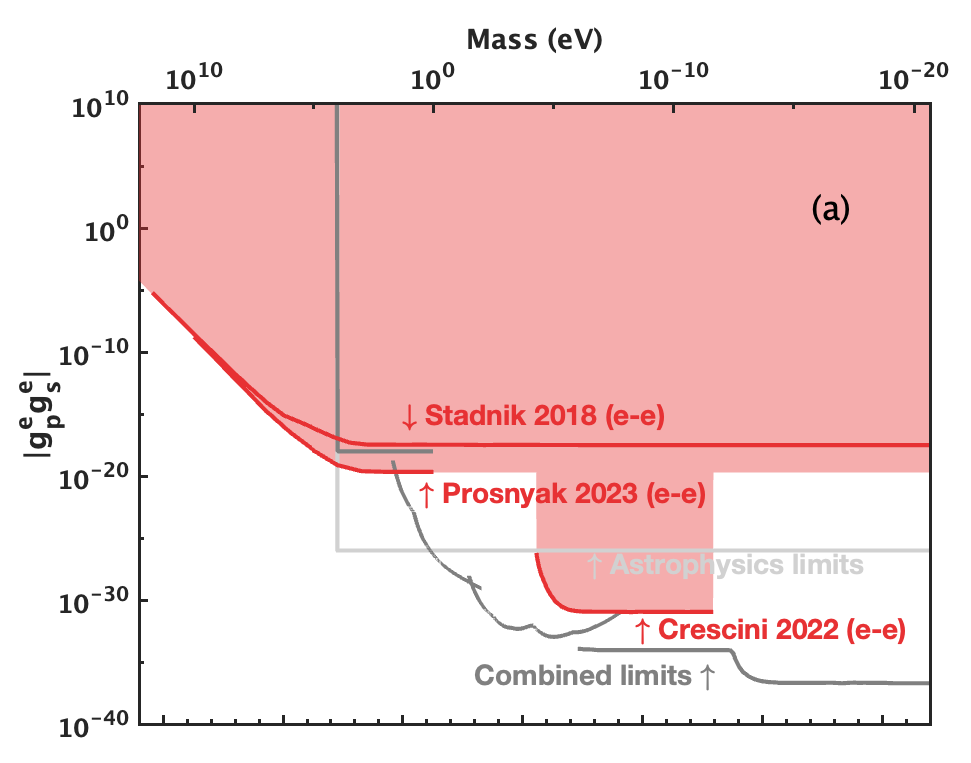
\includegraphics[width=0.48\textwidth]{Fig13_gpgs_a.eps}
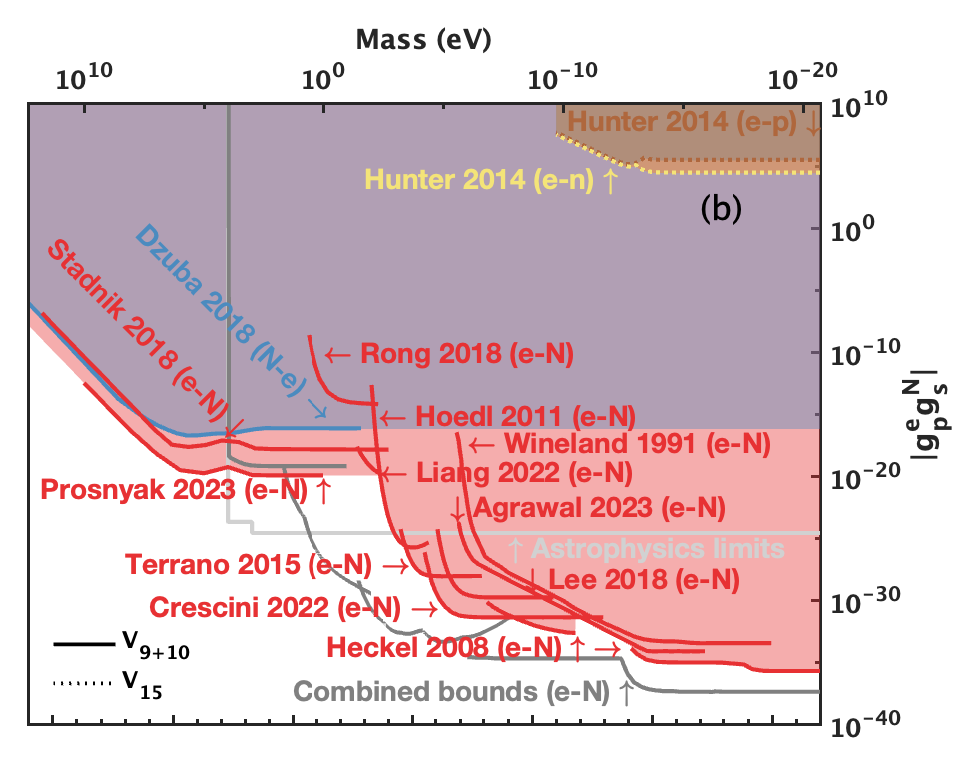
\includegraphics[width=0.48\textwidth]{Fig13_gpgs_b.eps}
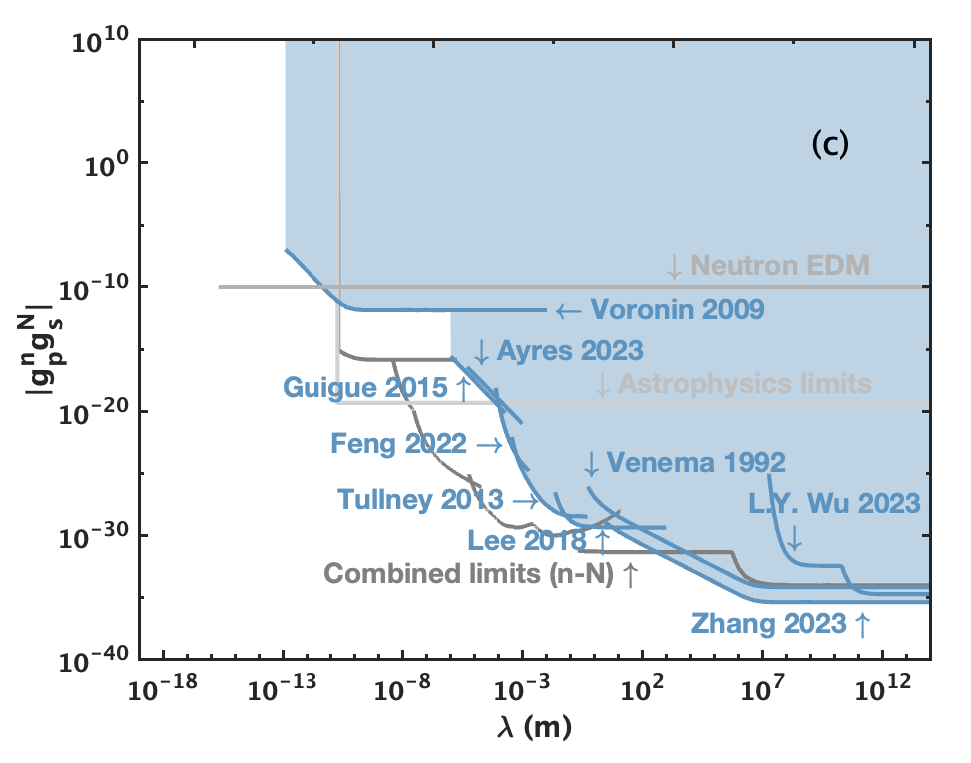
\includegraphics[width=0.48\textwidth]{Fig13_gpgs_c.eps}
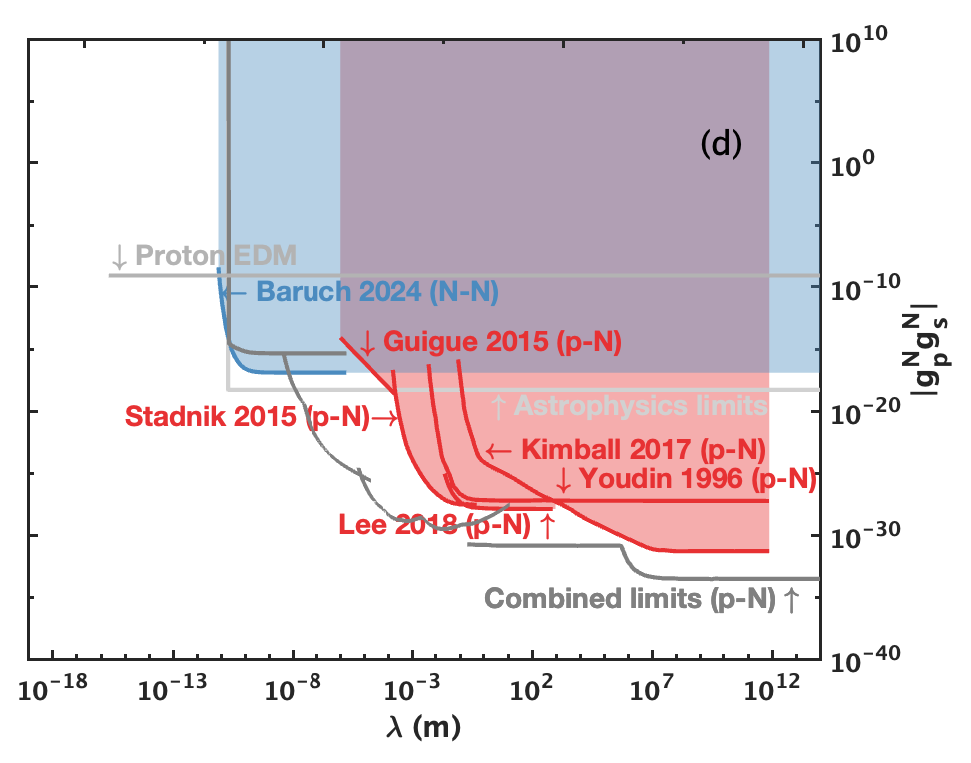
\includegraphics[width=0.48\textwidth]{Fig13_gpgs_d.eps}
\end{center}
\caption{Constraints, depicted by coloured regions, on the coupling constant product $g_p g_s$ as a function of the interaction range $\lambda$ shown on the bottom x-axis. 
The top x-axis represents the new spin-0 boson mass $M$. 
Here, the subscripts $p$ and $s$ denote the pseudoscalar and scalar couplings, respectively. 
Constraints shown for \textbf{(a)} $e$-$e$, \textbf{(b)} $e$-$N$, \textbf{(c)} $n$-$N$, \textbf{(d)} $p$-$N$ couplings. 
Results include $V_{9+10}$ (solid line) and $V_{15}$ (dotted line) terms. 
Combined bounds (solid, dark grey line) and astrophysical bounds (solid, light grey line) are elaborated in Appendices\,\ref{appendix_V1} and \ref{appendix_comp.}. In addition to the depicted bounds, \citet{agrawal_searching_2023} also placed constraints on the $V_{9+10}$ term for the exotic interaction between $\mu$ and $N$.
}\label{gpgs-fig}
\end{figure*}


%\LC{Comments for Fig.\,\ref{gpgs-fig}}.%\YS{{\color{red} The ``Combined bounds'' curve containing $g_s^e$ in subfigure (a) may need to be updated. Please see the discussion around Eq.~(\ref{gse-alpha}).}} \LC{Yes,  Combined bounds and Astrophysical results already updated.} 
%\YS{Thank you, Lei! I think the udpated bounds look mostly good.}
%\YS{Just to double-check: Should the combined bounds curves in (a) join up continuously at a mass of $\sim 10^2$\,eV?} \LC{no, there is a gap which also can be seen in Fig. 17.} \YS{OK, I see now. Thank you!}
%1. \YS{Should we truncate the combined bounds in (d) at a mass of $\sim 10^4$\,eV where they intersect the astrophysical limits line (and remove the tail at higher masses)?} %\LC{Why should we truncate? Why only this one?} {\color{green}YS: When we go to boson masses bigger than $\sim 10^4$\,eV, the astrophysical bounds rapidly diminish (according to a step function as we show in the figures), so the combined astro-lab bound would also deteriorate rapidly (like the same step function). It might be possible to use the purely $V_1$ bound from the ``molecular spectroscopy (N-N)'' curve in Fig.~\ref{V1-fig}, but that bound would be much weaker. We don't do this in the other subfigures, so I'm not sure if it makes sense to do this in subfigure (d) alone.} 
%\LC{I see, will do it soon.}\LC{Done}
%\YS{By the way, in Fig.~\ref{V1-fig}, which paper and fermion combination does the solid purple curve in the mass range $10^2 \sim 10^7$\,eV belong?} \LC{These are a few Neutron scattering papers, I have added a label there. }
%\YS{Could we add/restore the subfigure label (a) in the top-left subfigure?} \LC{done}
%\YS{Is it possible to use a darker shade of grey for the combined bounds in subfigures (b), (c) and (d) to match the shade used in subfigure (a), which has stronger differentiation from the astrophysical bounds line?} \LC{done}
%2.\YS{The bounds ``Dzuba 2018 (N-e)'' in subfigure (b) can be extended to boson masses greater than $10^8$\,eV using equation (18) therein.} \LC{Ok, will update}\LC{Done}
%\YS{In subfigure (c), could we update the label ``Wu 2023'' to ``L.\,Y.\,Wu 2023'' to avoid possible confusion with the other two Wu 2023 papers?} \LC{The problem is we have not enough space there for two more letters here. Since it is the only Wu in $g_pg_s$, maybe it is fine to use only Wu?}




%3. \YS{Is it possible to double-check the Venema 1992 bound in subfigure (c)? It looks about an order of magnitude weaker than what I infer from the original paper using their bound on $D$(neutron).} \LC{I checked, we take the data from \citet{ohare_cornering_2020} which originally from \citet{safronova_search_2018}. We take data correctly, so it could be \citet{safronova_search_2018} give an wrong result. Shall we correct them?}\YS{: I think it's generally safer to get the limits from the original source, unless later works explicitly pointed out some sort of error in the original paper. Using the relations in \cite{venema_search_1992}, I find the bound $g_p^n g_s^N = 8 \pi \hbar c m_n D (\textrm{neutron})$ < 7 \times 10^{-35}$.} \LCa{Ok, many thanks, we update the data, cited from \cite{zhang_search_2023} which I believe matches the value you found.}

%\YS{In subfigure (d), it looks like the $p$-$N$ bounds from Guigue 2015 and Lee 2018 may have been strengthened (instead of weakened) by a factor of 30 compared to their respective $n$-$N$ bounds in subfigure (c). Could we please check this?}\LC{Yes, we divided them by factor 32 to transfer the constraints for p-N from n-N before. Corretced now.} 

%4. \YS{Looking at the curve ``Stadnik 2015 (p-N)'' in subfigure (d), I think we made an error in our original paper \cite{stadnik_nuclear_2015}: in obtaining the $p$-$N$ bound in figure 1 there, it looks like we took the projected curve 9 from figure 3 of \cite{tullney_constraints_2013} when we should have taken curve 8 instead. I'm not sure how to proceed in this situation. In principle, it is easy to correct the shape of the curve with an explanation in the text, but that might not be in the spirit of this review. Or we could remove the curve altogether (though that would leave us with a big gap in that mass range).} \LC{Dima says it is ok we include the corrected result. We can add an foot note or a sentence to explain if you think necessary. Could you tell me how to update or send me the data?}  {\color{red}YS: Thank you for checking with Dima about this, Lei. I like this approach. In order to obtain the correct ``Stadnik 2015 (p-N)'' curve in Figure~\ref{gpgs-fig}(d), we need to weaken/rescale the ``Tullney 2013'' curve in Figure~\ref{gpgs-fig}(c) for the n-N coupling by a factor of 9 (i.e., shift the curve up by almost one order of magnitude). 
%I agree it would be nice to explain this correction in the main text in Sec.~\ref{subsec_g_Pg_S_p-N}.} \LCa{Dear Zhenia, I have updated the line. However, I just noticed we do not have content about the paper \citet{stadnik_nuclear_2015}, would you like to draft a few sentence in Sec.\,\ref{subsec_g_Pg_S_p-N} about it. }
%\YS{Dear Lei, Thank you for updating the line in the figure. I've drafted a few explanatory sentences in the main text (marked in cyan colour). I noticed that some of the shaded light red regions in Fig.~\ref{gpgs-fig}(d) extend below the red lines of Guigue 2015, Stadnik 2015 and Lee 2018 - would it be possible to check and (if needed) adjust these shaded regions?} \LC{Dear Zhenia, many thanks! Yes, we just update the shaded area.}


%\YS{In subfigure (d), the crossover point between the Kimball 2017 and Youdin 1996 curves looks a bit unclear. In figure 8 of \cite{jackson_kimball_constraints_2017}, the Kimball 2017 result looks like it's an approximately straight line when cutting through the Youdin 1996 curve, but here it looks like there is a discontinuity across the Youdin 1996 line. Could we please check this? \LC{That is true, we have updated the data.}} 
%\YS{Should we change the generic y-axis labels $|g_p g_s|$ in subfigures (a) and (d) to $|g_p^e g_s^e|$ and $|g_p^p g_s^N|$, respectively?} \LC{will done}
%\YS{Should we also add identifying labels to the ``Combined limits'' curves in the subfigures for clarity; e.g., in subfigure (a), ``Combined limits (e-e)''?} \LC{ok} 

%Constraints [shaded light blue (red, green, orange and gray)] to the coupling constant product $g_p g_s$ as a function of the interaction range $\lambda$ shown on the bottom x-axis. Constraints from $V_{9+10}$, $V_{15}$ are represented by solid, dotted lines, respectively. \textbf{(a)} 
%The faint (gray) lines are constraints from $V_{2}$ for $g_A^eg_A^e$ in (a), shown in (b-d) for reference.
%\YS{There are some other known bounds in the literature. Laboratory EDM bounds on the nucleon-nucleon pseudoscalar-scalar coupling from \citet{mantry_distinguishing_2014} are at the (conservative) level $g_s g_p \lesssim 10^{-9}$.} 
%\LC{ok, I plan to draw a constraint line in sub-figure (d) with $g_p^Ng_s^N=10^{-9}$. But what should be the x-axis range? $\lambda=10^{-10}$\,m is mentioned in the bottom of page 9 of \citet{mantry_distinguishing_2014}. (Updated 16 April: Derek added a paragrah about this paper and suggests it maybe fine to leave it out in the figure.) Updated 16 April: We may instead add the most recent N-N result from \cite{baruch_constraining_2024}? The question is can we direct plot their $g_pg_s$ constraints in our figure, they have some extra factor $N,Z,B$ in their Eq.\,(3). } 
%\YS{Thank you for the updates! I agree now that it's fine leave out the \cite{mantry_distinguishing_2014} constraints from the figure, since we now have the much stronger and more robust bounds of \cite{baruch_constraining_2024}. I think it's fine to keep the bound in \cite{baruch_constraining_2024} as-is: the interaction constants in their Eq.~(1) are the same as ours, while their monopole-dipole potential in Eqs.~(2,3) is simply summed over the nucleon contents of the two nuclei. }
%\YS{Should we also present bounds from proton and neutron EDM here as well (of the type shown in Figure 2 of \cite{baruch_constraining_2024}, reference [24] therein), which should apply to boson masses up to the nucleon mass?} \LC{I'm not sure. Does pEDM sets constraints for exotic interaction between protons? }
%\YS{In principle, these pEDM and nEDM bounds are similar in spirit to the $g$-factor-based bounds that we present in some of our main results graphs. That is, the pEDM and nEDM bounds arise from quantum loop-level processes involving a spinless boson. The specific diagrams are a bit different compared to those for the $g$-factor in Fig.\,\ref{yan2019-fig} though - see, e.g., Figure 1 of \cite{stadnik_improved_2018} for the analogous diagrams for the eEDM.} 
%{\color{red}YS [Update]: More discussion of this point appears below at the end of Sec.~\ref{subsec_g_Pg_S_p-N}.} 
%There were new laboratory bounds on $g_s^N g_p^n$ recently reported in \citet{wu_new_2023}. \LC{ok, in the figure now.}
%Regarding the (apparently) two separate lines for Arvanitaki 2014 shown in the figure -- technically, these aren't bounds, but rather projections for suggested future experiments, so I would propose to remove these Arvanitaki 2014 lines from the figure. \LC{ok, removed from here.}
%\YS{A similar comment to other places: the relevant constraints should be extended to cover the mass range shown. \LC{will update the figure, however, sometimes the paper will define a range, thus we extend if it is clearly stated in their paper or the author requires it.}}
%\DK{Even though the result from \citet{venema_search_1992} has recently been superseded by the measurement of \citet{zhang_search_2023}, I still think it is worth including that limit in the (c) plot since it was such a seminal result.}\LC{Ok, added.}


%%%%
%\subsubsection{$e$-$e$}
\subsubsection{\texorpdfstring{$e$-$e$}{e-e}}
% \& {\color{red}$\mu$-$\mu$} \YS{I couldn't find any discussion of $\mu-\mu$ in this subsection or in the main results figure}} 

We first turn our attention to the monopole-dipole lepton-lepton coupling for the fermion pair $e$-$e$, shown in Fig.\,\ref{gpgs-fig}\,(a). 

\citet{stadnik_improved_2018} present constraints on $g_p^e g_s^e$ based on the $V_{9+10}$ term by calculating axion-exchange-induced atomic EDMs using the relativistic Hartree-Fock Dirac method and then deriving limits from existing molecular EDM experiments. 
\citet{prosnyak_updated_2023} obtained constraints on $g_p^eg_s^e$ using the latest experimental result for HfF$^+$ cations \cite{roussy_improved_2023}. 
%\DK{These results from \citet{prosnyak_updated_2023} don't seem to appear on the plot in Fig.\,\ref{gpgs-fig}.}\LC{Added now.} 
Their results are more stringent than the constraints from \citet{stadnik_improved_2018}, as well as their earlier result \cite{maison_axion-mediated_2021}, which investigated YbOH (not plotted for clarity).
\citet{crescini_search_2022} obtained constraints for $g_p^eg_s^e$ from the $V_{9+10}$ potential term in the range $3 \times 10^{-3} \,\textrm{m} <\lambda < 10^{5} \, \textrm{m}$
%$10^{-2}<\lambda < 3\times10^{5}$ \YS{In their figure, the mass range of the experiment looks more like $3 \times 10^{-3} \,\textrm{m} <\lambda < 10^{5} \, \textrm{m}$ -- Could we double-check please?} \LC{You are right, corrected.}
by scaling limits on the electron-nucleon interaction $g_p^eg_s^N$ by measuring the change of the magnetization of a paramagnetic crystal when the distance to a lead mass is modulated under the assumption that $A =2.5Z$ for the source mass. 
More details concerning the work of 
\citet{stadnik_improved_2018}; \citet{crescini_search_2022}; \citet{prosnyak_updated_2023}
%\citet{stadnik_improved_2018,crescini_search_2022,prosnyak_updated_2023} 
are discussed later in this section.

%\citet{yan_constraining_2019} studied the muon's EDM and establish a constraint for $g_P^{\mu}g_S^{\mu}$ of $V_{9+10}$ (for futher discussion of this result, see Sec.\,\ref{subsec_g_Ag_A}).

%\citet{hunter_using_2014} employed a model of electron spins in Earth to explore long-range velocity-dependent interactions between spins related to the exchange of ultralight vector bosons and used existing laboratory experiments to set constraints on $V_{15}$. 
%Here, using the theoretical framework discussed in earlier sections, we translate \citet{hunter_using_2014}'s constraints on $V_{15}$
%\YS{via the $V_{15}$ term (I just realised that we don't include the $V_{15}$ term in our vector-vector potential in Eq.~(\ref{vector-vector_potential}) -- should we address this?).} \LC{The question is $V_{15}$ exist in $V_{VV}$? I do not find any place $f_{15}$ is related with $g_Vg_V$ anywhere in \citet{dobrescu_spin-dependent_2006} or \citet{fadeev_neue_2018}. Now I think perhaps \citet{hunter_using_2014} wrote his equations wrong? If so, we can change the above two $g_V^eg_V^e$ to $V_{15}$. }
%\YS{I also don't recall a $V_{15}$ term arising in the vector-vector potential. Maybe Hunter confused the vector-vector potential with the tensor-pseudotensor potential (which is also mediated by a spin-1 boson)? In any case, I agree with your suggestion to simply change $g_V^e g_V^e$ in the text above to $V_{15}$.} 
%to constraints on $g_p^eg_s^e$ and present them in Fig.\,\ref{gpgs-fig}\,(a), see Sec.\,\ref{g_Vg_A_e-n} for further discussion. 
%In addition, \citet{ji_new_2018} carried out an experiment using iron-shielded SmCo$_5$ spin sources and a SERF comagnetometer (see Sec.\,\ref{Sec:EXP.METH.1}) to study the $V_{15}$ term and set constraints on $f_{15}$, which we have converted to a limit on $g_p^e g_s^e$ and presented in Fig.\,\ref{gpgs-fig}\,(a). 


%\LC{Check all Victor's results and make sure to extend all of them.} 

%\YS{ I think it would be worth adding $e - \mu$ bounds here too.}   \LC{We do not have such a limit here. Maybe in other section?} \LC{YS: Maybe in another section.}


%%%%
%\subsubsection{$e$-$N$}
\subsubsection{\texorpdfstring{$e$-$N$}{e-N}}
\label{gpgs_e-N}

In the case of $e$-$N$ couplings, as shown in Fig.\,\ref{gpgs-fig}\,(b), the strongest bounds in the interaction ranges $\lambda>10^{6}$\,m and $10\,\textrm{m} < \lambda < 10^{4}$\,m are set by the experiment of \citet{heckel_preferred-frame_2008} using a spin-polarized torsion pendulum (see Sec.\,\ref{METH1.SENS.MS}). 
Details about the experiment of \citet{heckel_preferred-frame_2008} can be found in Sec.\,\ref{subsec_g_Ag_V}. 
Another important experiment, covering the range $\lambda>4.9\times 10^{-4}$\,m, is that of \citet{terrano_short-range_2015} who also use a spin-polarized torsion-pendulum to search for spin-mass interactions. 
Details about the work of \citet{terrano_short-range_2015} are discussed in Sec.\,\ref{subsec_g_Pg_P}. 
In the range $4 \times 10^{-5} \, \textrm{m} < \lambda < 4.9\times 10^{-4}$\,m, \citet{hoedl_improved_2011} also conducted a spin-polarized torsion-pendulum experiment to search for exotic spin-dependent interactions. 
The experiment of \citet{hoedl_improved_2011} differed from those of \citet{heckel_preferred-frame_2008} and \citet{terrano_short-range_2015} in that the latter experiments used mu-metal shielding to minimize torques from stray magnetic fields, whereas \citet{hoedl_improved_2011} used a magnetically unshielded torsion pendulum in order to bring the source mass in closer proximity to the spins, thereby probing shorter-range forces than other experiments, including those in \citet{ni_search_1999,hammond_new_2007}. 
%\citet{hoedl_improved_2011} interpreted the results of their experiment as a limit on $g_p^eg_s^a$, where $g_s^a=(Z+N)g_s^N$, and $Z$ and $N$ are the numbers of protons and neutrons, respectively. To plot $g_p^eg_s^N$ in this review, the original $g_p^eg_s^a$ data were rescaled by $Z+N=28$ for silicon. \YS{Don't \citet{hoedl_improved_2011} already present a bound on $g_p^e g_s^N$ in their Figure 3? Do we need to rescale again?} \LC{You are right. I have updated it.}

%to search for low-mass pseudoscalars, such as the axion, which can cause macroscopic parity- and time-reversal-invariance-violating (PT violating) forces described by the $V_{9+10}$ potential. 
%This apparatus consisted of a nonmagnetic torsion pendulum suspended on a tungsten fiber between two halves of a stationary split toroidal electromagnet. 
%As the pendulum was unshielded, it enabled the setting of constraints at a shorter distance than previous PT violating searches \cite{ni_search_1999,hammond_new_2007} which used magnetic shields to reduce background magnetic forces. 
%The PT violating force between the polarized electrons in the electromagnet and the unpolarized silicon atoms in the pendulum generated a torque on the pendulum that was dependent on the magnetic field. This PT violating force has a unique signature related to the geometrical factor of approximately $cosh(x,\lambda)$, where $x$ is the distance between the pendulum and the symmetry plane between the magnet halves, and thus can be distinguished from other spurious magnetic-field-dependent effects such as torques caused by impurities and diamagnetic torques, the effects already minimized by their pendulum design. 
%As no evidence for a PT violating force was found in their experimental results, \citet{hoedl_improved_2011} improved the bounds on such a force between polarized electrons and unpolarized nucleons over most of the classical QCD axion window. Initially, these authors established limits on $g_P^eg_S^a$, where $g_S^a=(Z+N)g_S^N$ and $Z$ and $N$ are the proton and neutron numbers. To plot $g_p^eg_s^N$ in this review, the original $g_P^eg_S^a$ data was rescaled by $Z+N=28$ for silicon.

In the range $10^{4} \, \textrm{m} < \lambda < 10^{6} \, \textrm{m}$, \citet{agrawal_searching_2023} provide the most stringent limit on $g_p^e g_s^N$, based on results from electron $g-2$ \cite{hanneke_new_2008,hanneke_cavity_2011} and storage ring experiments. The exotic interaction between Earth's nucleons and the electrons induces an additional contribution to the electron precession frequency with respect to the Standard Model prediction. Thus, various types of experiments, originally designed to precisely measure the magnetic and electric dipole moments of protons, muons, and electrons, could serve as precision probes of monopole-dipole interactions \cite{vergeles_general_2023}. This work also provides the constraints on $g_p^{\mu} g_s^N$ based on muon $g-2$ experiments and offers a projection for $g_p^p g_s^N$ based on proton storage ring experiments. See more in Sec.\,\ref{METH2.g-factor}.
%\sout{In the range $3 \times 10^{5} \, \textrm{m} < \lambda<10^{6}$\,m, }
%\LC{
Previously, in a similar range, 
%} 
\citet{wineland_search_1991} 
%searched for an exotic dipole-monopole interaction, $V_{9+10}$, by examining the hyperfine resonances of trapped and cooled $^9$Be$^+$ ions, see further discussion in Sec.\,\ref{METH2.PM.TI}. 
%\YS{
placed the most stringent limit on the dipole-monopole interaction $V_{9+10}$ by examining the hyperfine resonances of trapped and cooled $^9$Be$^+$ ions and using Earth as the source body, see Sec.\,\ref{METH2.PM.TI} for further discussion.
%} 

As noted by \citet{hunter_using_2013}, Earth contains about $10^{42}$ spin-polarized electrons due to the geomagnetic field (also discussed in Sec.\,\ref{subsec_g_Ag_V}). 
For length scales $10^{3} \, \textrm{m} < \lambda < 10^{11}$\,m, \citet{hunter_using_2014} used a model of the spin-polarized geoelectrons to set constraints on $g_p^eg_s^p$ and $g_p^eg_s^n$ based on the exotic velocity-dependent potential term $V_{15}$. 
Recently, \citet{poddar_constraints_2023} pointed out that these electrons can interact with the unpolarized nucleons in the Sun, leading to a force caused by the monopole-dipole potential between the Sun and Earth. 
This force can affect Earth's motion. 
\citet{poddar_constraints_2023} used the well-measured perihelion precession of the Earth to set limits on the pseudoscalar-scalar electron-nucleon coupling at the level $g_p^e g_s^N \lesssim 2 \times 10^{-16}$ for the range $\lambda>10^{11}$\,m. 
%\LC{remove this part:, and also derived stringent limits by considering Earth's perihelion precession in combination with limits from stellar cooling in the spirit of \citet{raffelt_limits_2012}.} 
%\LC{add this: 
However, \citet{clayburn_spherically_2025} later pointed out that the constraints of \citet{poddar_constraints_2023} must be relaxed by a factor of about 2000, since the net spin polarization of the Earth’s electrons is low. 
%}

%\LC{New content, need read: Note in the range of $\lambda>10^{11}$\,m, \citet{poddar_constraints_2023} directly constrained the pseudoscalar-scalar electron-nucleon coupling at the level $g_p^e g_s^N = 1.8 \times 10^{-16}$ from the consideration of the perihelion precession of Earth. They also places a stringent constraint on $g_p^e g_s^N$ from the combination of the consideration of the perihelion precession of Earth for the scalar-nucleon coupling and red giant star evolution for the pseudoscalar-electron coupling.}

%\DKDel{Additionally, \citet{wineland_search_1991} studied the dipole-dipole $V_{3}$.  Some early results, such as those of \citet{lamoreaux_new_1986,ramsey_tensor_1979} are listed in \citet{wineland_search_1991} for comparison.} \DK{Shouldn't these already be discussed in other sections? Not necessary here I think.}

%In the range of 3$\times10^{5}<\lambda<10^{6}$\,m, \citet{wineland_search_1991} searched for an exotic dipole-monopole interaction, $V_{9+10}$, by examining the hyperfine resonances of approximately 5000 trapped and cooled $^9$Be$^+$ ions. The nucleons in the Earth served as the source, while the ions acted as a spin sensor. An applied magnetic field was switched between being directed either parallel or antiparallel to the direction of gravity, and any contribution of the exotic interaction would be revealed by a difference in the resonance frequency of the transition between the $^2 S_{1/2} \ket{F=1,M=0}$ and $^2 S_{1/2} \ket{F=1,M=-1}$ states of the $^9$Be$^+$ ions. Additionally, \citet{wineland_search_1991} studied the dipole-dipole $V_{3}$ interaction with the same ions, using electron spins in an electromagnet as the dipole source. To control for systematic effects, the electromagnet was replaced with a superconducting solenoid that whose magnetic field did not result from polarized spins. \citet{wineland_search_1991} suggested that the sensitivity of the experiment could be improved with longer coherence times and more ions.
%Some early results, such as those of \citet{lamoreaux_new_1986,ramsey_tensor_1979} are listed in \citet{wineland_search_1991} for comparison. 
%\DK{These on't seem to be shown on the plot.} \LC{I mean they are listed in \citet{wineland_search_1991}.} %\LC{Q: Should they be considered? Why the \citet{safronova_search_2018} only cite two of the results from $V_{9+10}$? But not others?}

%\citet{wineland_search_1991} carried out measurements on trapped $^9$Be$^+$ ions as an applied magnetic field was reversed relative to the local gravitation field $\boldsymbol{g}$: the resulting frequency shift between the $^9$Be$^+$ $^2 S_{1/2} \ket{F=1,M=0}$ and $^2 S_{1/2} \ket{F=1,M=-1}$ states was constrained to be < 13.4\,\textmu{Hz}.

\citet{crescini_search_2022}, as part of the QUAX experimental program (\citealp{ruoso_quax_2016}; \citealp{crescini_quax-gpgs_2017}),
%\cite{ruoso_quax_2016,crescini_quax-gpgs_2017},
conducted a search for spin-dependent interactions between lead masses (acting as the unpolarized ensemble of nuclei and electrons) and two paramagnetic Gd$_2$SiO$_5$ (GSO) crystals at $T=4.2$~K (acting as the spin-polarized ensemble). 
A set of 24 cylindrical lead masses (height = 6~cm, diameter = 5~cm) were arranged on a 1\,m diameter disc which was rotated above the pair of GSO crystals. 
The minimum separation between the GSO crystals and the lead masses was $\approx 3.5$\,cm. 
The GSO crystals were surrounded by two layers of mu-metal shielding and two additional layers of superconducting shielding. 
A monopole-dipole interaction between the lead masses and the spins in the GSO crystals would induce a change in the GSO magnetization \cite{landau_theoretical_2010} as the positions of the lead masses relative to the GSO crystals changed. The magnetization of the GSO crystals was measured with a state-of-the-art dc-SQUID (superconducting quantum interference device) magnetometer \cite{ni_scheme_1996}. 
%For the interaction range between $10^{-2}$\,m and 10\,m, \citet{crescini_search_2022} improved the sensitivity and constraints on spin-dependent interactions compared to their prior work \cite{crescini_improved_2017}, and for the range $10^{4}\,\textrm{m} < \lambda <  3\times10^{5}$\,m, their experiment established the most stringent constraint on $e$-$N$ monopole-dipole couplings. 
%\YS{It looks like \citet{crescini_search_2022} improved over not only over \cite{crescini_improved_2017} in the range between $10^{-2}$\,m and 10\,m, but also compared to all other laboratory bounds (including Heckel 2008). Maybe we could update this sentence to read as follows?  
For the interaction ranges $10^{-2}\,\textrm{m} < \lambda <  10$\,m,
%\LC{\sout{and $10^{4}\,\textrm{m} < \lambda <  3\times10^{5}$\,m}}, 
\citet{crescini_search_2022} established the most stringent constraint on the $e$-$N$ monopole-dipole coupling, including improved sensitivity compared to their prior work \cite{crescini_improved_2017}.
%} \LC{Yes, thanks!}
Note that similar techniques were used in earlier searches by \citet{vorobyov_new_1988} and \citet{ni_search_1999}. \citet{crescini_search_2022} pointed out that their experimental method should be able to be improved by using an LC pickup coil \cite{vinante_dc_2001} or crystals with a higher magnetic susceptibility. If these improvements are successfully implemented in future experiments, the sensitivity of this method should be able to surpass the combined bounds.



In the range $\lambda < 4 \times 10^{-5}$\,m, \citet{stadnik_improved_2018} established limits on the pseudoscalar/scalar electron-nucleon interaction constant product $g_p^e g_s^N$ and electron-electron interaction constant product $g_p^eg_s^e$ mediated by ALPs. 
The $P,T$-violating potential $V_{9+10}$ can generate EDMs in atoms and molecules through the mixing of atomic states with opposite parity, see more in Sec.\,\ref{METH2.EDM}. 
\citet{stadnik_improved_2018} performed theoretical calculations of atomic EDMs using the relativistic Hartree-Fock-Dirac method, including electron core polarization corrections. 
Based on the experimental bounds on the EDMs of various atoms and molecules, including $^{133}$Cs, $^{205}$Tl, $^{129}$Xe, $^{199}$Hg, $^{171}$Yb$^{19}$F, $^{180}$Hf$^{19}$F$^+$, and $^{232}$Th$^{16}$O, \citet{stadnik_improved_2018} determined limits on $g_p^eg_s^N$ and $g_p^eg_s^e$ for a range of ALP masses. 
The most stringent limits on high-mass ALPs were derived from Hg and ThO, while the most stringent limits on low-mass ALPs were obtained from HfF$^+$. 

Building on the work of \citet{stadnik_improved_2018}, \citet{dzuba_new_2018} established further constraints on the interaction between an unpolarized electron and a polarized nucleon, denoted by $g_p^Ng_s^e$, which can induce EDMs of diamagnetic atoms. 
In contrast, the previous research \cite{stadnik_improved_2018} focused on the atomic EDMs of paramagnetic atoms. \citet{dzuba_new_2018} used the relativistic Hartree-Fock-Dirac method to calculate the atomic EDM of $^{199}$Hg, $^{129}$Xe, $^{211}$Rn, and $^{225}$Ra, and combined the results with experimental measurements of EDMs in these atoms to set constraints on the product of coupling constants $g_p^Ng_s^e$ for a wide range of ALP masses. 
The most stringent limits for any ALP mass $m_a \gtrsim 10^{-2}\,\textrm{eV}$ were derived from $^{199}$Hg. 
Compared to the constraints from macroscopic-scale experiments (\citealp{serebrov_new_2009}; \citealp{petukhov_polarized_2010}; \citealp{tullney_constraints_2013}; \citealp{bulatowicz_laboratory_2013}; \citealp{afach_constraining_2015}),
%\cite{serebrov_new_2009,petukhov_polarized_2010,tullney_constraints_2013,bulatowicz_laboratory_2013,afach_constraining_2015}, 
which reported constraints on the coupling parameters $g_p^ng_s^N$, \citet{dzuba_new_2018} provided significantly improved laboratory limits for $\lambda <2 \times 10^{-5}$\,m.

More recently, \citet{prosnyak_updated_2023} have used experimental data on the static $P,T$- violating molecular EDM of HfF$^+$ \citet{roussy_improved_2023} to constrain virtual ALP exchange between electrons and nuclei. 
This has resulted in a constraint on $g_p^e g_s^N$ that is more stringent than the one \citet{stadnik_improved_2018} derived from the ThO EDM experiment \citet{acme_collaboration_improved_2018}. 
%\LC{Updated content: 
Additionally, \citet{maison_electronic_2021} have calculated the sensitivity coefficients for a proposed YbOH experiment \cite{kozyryev_precision_2017}. 
%}
%\YS{If I understood correctly, \citet{maison_electronic_2021} calculated sensitivity coefficients for a proposed/future experiment using YbOH, rather than placed constraints. Could we please check this and update the previous (and next) sentence as needed?} \LC{Yes, you are right. I have rewritten the sentence. }
%However, since this has been superseded by \citet{prosnyak_updated_2023}, it is not included in Fig.\,\ref{gpgs-fig} for the sake of clarity. 

In the range $10^{-7} \, \textrm{m} < \lambda < 2.3 \times 10^{-5}$\,m, \citet{rong_searching_2018} showed that a near-surface NV center in a diamond can be used as a quantum sensor to detect the monopole–dipole interaction $V_{9+10}$. 
In the range $6\times 10^{-6} \, \textrm{m} < \lambda <4.5 \times 10^{-5}$\,m, \citet{liang_new_2022} further improved the constraints using an ensemble of NV centers. 
Both of these sets of constraints have been surpassed by the EDM searches described above. 

%In the range of $10^{-7}<\lambda <2.3 \times 10^{-5}$\,m, \citet{rong_searching_2018} showed that a near-surface NV center in a diamond can be used as a quantum sensor to detect the monopole–dipole interaction $V_{9+10}$. The electron-nucleon interaction between the electron spin of the NV center and nucleon in a fused silica half-ball lens is interpreted as an effective magnetic field and can be detected by the quantum sensor. Therefore, \citet{rong_searching_2018} set a limit on the electron–nucleon coupling $g_p^eg_s^N$.



For other earlier constraints on $g_p^e g_s^N$ that are not presented in Fig.\,\ref{gpgs-fig}\,(b), such as earlier bounds from torsion-pendulum and comagnetometry experiments, such as \citet{youdin_limits_1996}; \citet{ni_search_1999}; \citet{hammond_new_2007}; \citet{crescini_improved_2017},
%\citet{youdin_limits_1996,ni_search_1999,hammond_new_2007,crescini_improved_2017}, 
one can find a collection of references in the papers of \citet{stadnik_improved_2018}, \citet{safronova_search_2018}, and \citet{jackson_kimball_probing_2023}.

In addition, \citet{hunter_using_2014} employed a model of electron spins in Earth to explore long-range velocity-dependent interactions between spins related to the exchange of ultralight vector bosons and used existing laboratory experiments to set constraints on $V_{15}$. 
Here, using the theoretical framework discussed in earlier sections, we translate \citet{hunter_using_2014}'s constraints on $V_{15}$
to constraints on $g_p^eg_s^n$ and $g_p^eg_s^p$ and present them in Fig.\,\ref{gpgs-fig}\,(b), see Sec.\,\ref{g_Vg_A_e-n} for further discussion. 


%%%%
%\subsubsection{$n$-$N$}
\subsubsection{\texorpdfstring{$n$-$N$}{n-N}}
\label{subsec_g_Pg_S_n-N} 

For monopole-dipole couplings between neutrons and nuclei, as shown in Fig.\,\ref{gpgs-fig}\,(c), the strongest bounds in the range $\lambda>10$\,m were established by \citet{zhang_search_2023}, who utilized a $^{129}$Xe-$^{131}$Xe-Rb clock-comparison-type atomic comagnetometer (Sec.\,\ref{METH1.SENS.AM}) to search for an exotic spin-dependent interaction between neutron spins and Earth. 
%\LC{
\citet{zhang_search_2023} measured the nuclear-spin precession frequency ratio of two Xe isotopes and its variation between field directions, indicating precession from non-magnetic effects like monopole-dipole coupling of the Xe spins to Earth. See more details in Sec.\,\ref{gpgs_spin-gravity}.
%}
%\LC{Replace the following: \citet{zhang_search_2023} measured the nuclear-spin precession frequencies of the two Xe isotopes in an applied magnetic field that was aligned parallel to Earth's rotation axis in order to reduce systematic errors caused by gyroscopic effects. The team then constructed the ratio of the two precession frequencies and repeated the measurements with the direction of the magnetic field reversed, measuring the difference between the ratios corresponding to the two different field directions. This difference is proportional to the magnitude of precession caused by non-magnetic effects, such as that arising from a monopole-dipole coupling of the Xe spins to Earth. The analysis of the data revealed no evidence of a monopole-dipole interaction.} 
Their experimental limits surpassed those from experiments by \citet{wu_new_2023} using spin-polarized neutrons and the Sun and Moon as the monopole sources (with Earth's rotation providing modulation). 
The experiment of \citet{zhang_search_2023} also surpassed the prior work of \citet{venema_search_1992} using a $^{199}$Hg-$^{201}$Hg comagnetometer, which had long held the record for the best sensitivity to long-range monopole-dipole couplings. 

Earlier, the same team had used their $^{129}$Xe-$^{131}$Xe-Rb comagnetometer to search for an interaction between the Xe spins and the nuclei of a cm-scale, nonmagnetic BGO crystal source mass, enabling them to search for a monopole-dipole interaction in the range $10^{-4} \, \textrm{m} < \lambda < 5 \times 10^{-4}$\,m \cite{feng_search_2022}. 
Their experiment improved on an earlier experiment by \citet{bulatowicz_laboratory_2013} using a similar $^{129}$Xe-$^{131}$Xe-Rb comagnetometer. 
\citet{feng_search_2022} noted that further improvement of their sensitivity is possible by using multipass cavity technique \cite{hao_herriott-cavity-assisted_2021} to enhance the signal-to-noise performance of the comagnetometer. 
Future experiments could also probe shorter distances by employing microfabrication techniques \cite{kitching_chip-scale_2018}.


%\citet{feng_search_2022} focused on the ratio R between the precession frequencies of the two Xe isotopes, $^{129}$Xe and $^{131}$Xe, correlated with the position of the BGO mass. R is expressed as $(\gamma_{129}B +X_{129})/(\gamma_{131}B +X_{131})$ where the $X_i$ denotes the frequency shift of the corresponding $^i$Xe isotopes due to exotic interactions, and $\gamma_{i}$ represents nuclear gyromagnetic ratio. In the measurement sequence, together with the position of the BGO mass, the bias field direction, and the pumping beam polarization are periodically switched.
%The comagnetometer system used by \citet{feng_search_2022} was previously utilized to search for the monopole-dipole interactions by \citet{bulatowicz_laboratory_2013}. However, \citet{feng_search_2022} employed a modulated Rb polarization scheme \cite{limes_3mathrmhetextensuremath-129mathrmxe_2018} and designed the measurement sequence to reduce the systematic effect. Thus, \citet{feng_search_2022} was able to provide improved constraints on the coupling constants of exotic particles that mediate monopole-dipole interactions compared to \citet{bulatowicz_laboratory_2013}. 


%[May 23] In the distance range including astronomical distances, \DB{This, at least partially, repeats the information in the paragraph above. Kindly consolidate} $2\times10^{10}<\lambda < 10^{14}$\,m, \DB{Where does the upper limit come from? Why not infinity, we need to state!} \citet{wu_new_2023} used the Sun/Moon as source masses and the Earth’s rotation as a modulation to search for exotic spin-dependent interactions. They set laboratory constraints on monopole-dipole interactions $V_{9+10}$ between spin-polarized neutrons and Earth. See also in Sec.\,\ref{subsec_g_Ag_V}.

%In the range of $\sim\,10^{-1}<\lambda < 10^{12}$\,m, \citet{venema_search_1992} measured the spin-precession frequencies of two isotopes of mercury,  $^{199}$Hg and $^{201}$Hg, as a way to search for exotic interaction generating spin precession about an axis directed along the local gravitational field $\boldsymbol{g}$.  
%The overall spin-precession frequencies for the two Hg isotopes are
%\begin{align}
%\Omega_{199} = \gamma_{199} B + \chi_{199} g \cos{\phi}~, \\
%\Omega_{201} = \gamma_{201} B + \chi_{201} g \cos{\phi}~, 
%\end{align}
%where $\gamma_i$ is the gyromagnetic ratio and $\chi_i$ is the so-called ``gyrogravitational ratio'' parameterizing the exoticinteraction (the subscripts $i$ denote the respective isotopes), and $\phi$ is the angle between $\mathcal{B}$ and $\boldsymbol{g}$.  
%There is no a-priori reason for the ratio $\chi_{199}/\chi_{201}$ to be the same as $\gamma_{199}/\gamma_{201}$, so the ratio $\sR = \Omega_{199}/\Omega_{201}$ generally depends on $B$ and $\phi$ if the $\chi_i$'s are nonzero, enabling a search for the monopole-dipole coupling.
%The work of \citet{venema_search_1992} illustrates the principles involved in a broad class of experiments that rely on optical measurements of spin precession of various atomic species in the gas phase [for reviews of these experimental techniques, see \citet{budker_optical_2013,budker_resonant_2002,budker_optical_2007}]. The limits were present previously in Fig.\,13 of Ref. \citet{safronova_search_2018}.


%In the range of $10^{-1}<\lambda < 10$\,m, \citet{lee_improved_2018} searched for light particles, such as ALPs, that possess CP-violating couplings to ordinary matter and placed constraints on $g_p^ng_s^N$ (and $g_p^eg_s^N$). They utilized a K-$^3$He self-compensating comagnetometer (see Sec.\,\ref{METH1.SENS.AM}) and movable Pb masses. 
%Similar to the previous discussion after Eq.\,\eqref{ANZ}, \citet{lee_improved_2018} termed the scalar coupling to unpolarized fermions to be $g_S^N$, assuming the coupling is identical for both neutrons and protons and is zero for electrons in the unpolarized mass. Furthermore, they also assumed the neutron to be 87\% polarized in $^3$He \cite{ethier_comparative_2013,friar_neutron_1990}.
%The limits on $g_p^ng_s^N$ set by \citet{lee_improved_2018} were improved by over two orders of magnitude in the axion mass range, in comparison to \citet{tullney_constraints_2013}.
%\citet{lee_improved_2018} also pointed out towards possible improvement by applying a more sensitive comagnetometer \cite{vasilakis_limits_2009} compared to the one \cite{kornack_nuclear_2005} used in the work of \citet{lee_improved_2018}.


In the interaction range $10^{-1} \, \textrm{m} < \lambda < 10$\,m, \citet{lee_improved_2018} searched for monopole-dipole couplings of $^3$He (and K) spins to 
%{\color{red}ordinary matter} \YS{
unpolarised source masses
%} 
and placed constraints on $g_p^ng_s^N$ (and $g_p^eg_s^N$). 
They utilized a K-$^3$He self-compensating SERF comagnetometer and movable Pb masses. 
%The comagnetometer contains overlapping ensembles of spin-polarized K and $^3$He, and during the experiment, it is operated at the compensation point, where the $^3$He magnetization cancels, to first-order, the applied magnetic field. This makes the system insensitive to ordinary magnetic fields yet highly sensitive to torques from exotic spin-dependent interactions experienced by $^3$He and K. 
\citet{lee_improved_2018} identified the scalar coupling to unpolarized fermions to be $g_s^N$ and assumed the coupling to be identical for both neutrons and protons and zero for electrons in the unpolarized mass [see the discussion after Eq.\,\eqref{ANZ}]. 
%The limits on $g_p^ng_s^N$ set by \citet{lee_improved_2018} improved by more than one order of magnitude compared to the previous constraints set by \citet{tullney_constraints_2013}. 

%\YS{Looking at the plots in the relevant papers, it looks like the improvement is up to (about) one order of magnitude. I'm not sure where we have more than 2 orders of magnitude improvement.} \LC{You are right. i have changed 2 orders to 1 order.}

%\LC{Note for myself: this is based on the comparison of the relative position of the limits of chu 2013.}

In the range around $5\times10^{-4} \, \textrm{m} < \lambda < 10^{-1}$\,m, \citet{tullney_constraints_2013} utilized 
%\WJDel{an ultra-sensitive low-field magnetometer} \WJIns{
a SQUID magnetometer
%} 
to detect the free precession of $^3$He and $^{129}$Xe nuclear spins and set constraints for $g_p^ng_s^N$ from $V_{9+10}$. See more details in Sec.\,\ref{Sec:EXP.METH.1}.
%In their experimental setup, an unpolarized cylindrical BGO crystal was used as a source, generating a pseudomagnetic field and thus giving rise to a shift in the precession frequency of the nuclear spin-polarized gases. The precession was measured with a magnetometer based on low-Tc SQUID, see also their earlier proposal \cite{burghoff_probing_2011}. 
%This approach avoided problems with light shifts, which appear in optical atomic magnetometry experiments (Acosta et al., 2006; Jackson Kimball et al., 2017; Kimball et al., 2013). 
\citet{tullney_constraints_2013} improved on the previous bounds (\citealp{chu_laboratory_2013}; \citealp{stadnik_nuclear_2015}; \citealp{youdin_limits_1996}) 
%(Chu et al., 2013; Stadnik and Flambaum, 2015; Youdin et al., 1996)
%on spin-dependent exotic interaction between polarized neutrons and unpolarized nucleons 
across most of the axion window.

In the range $10^{-6} \, \textrm{m} < \lambda < 10^{-4}$\,m, \citet{guigue_constraining_2015} searched for a monopole-dipole interaction between nucleons and hyperpolarized $^3$He based on the $V_{9+10}$ potential term. 
The nucleons in the walls of a $^3$He-filled glass cell served as the monopole source to generate a pseudomagnetic field. 
Helium spins evolving in the presence of the pseudomagnetic field would experience an additional longitudinal depolarization in addition to the usual depolarization mechanisms. 
Such an extra longitudinal depolarization was distinguished from the other standard contributions, such as atomic and wall collisions, by examining the longitudinal relaxation rate as a function of the applied magnetic field strength. 
The existence of a new boson would be revealed if a deviation in the behavior of the rate was observed and matched the calculated exotic-interaction-induced contribution to spin relaxation. 
%No evidence of an exotic depolarization channel was observed and based on this measurement, 
\citet{guigue_constraining_2015} improved upon the constraints on $g_p^ng_s^N$ by a factor of 20 compared to the preliminary experiment \citet{petukhov_polarized_2010} performed at the same Institut Laue-Langevin (ILL). 
The long relaxation time of the polarized gas (up to several days) contributed to the increased sensitivity of the newer experiment. 
Note that \citet{fu_limits_2011} proposed and carried out a similar experiment to that of \citet{guigue_constraining_2015}, but with a moveable cm-scale polytetrafluoroethylene (PTFE) mass as the monopole source. 

\citet{voronin_neutron_2009} used neutron diffraction in a non-centrosymmetric crystal to search for a sub-micron range monopole-dipole interaction. 
When neutrons travel through the crystal over time $\tau$, the $V_{9+10}$ potential would lead to precession of neutron spins around the reciprocal lattice vector $\boldsymbol{g}$ by an angle $\phi={2 V_{9+10} \tau}/{\hbar}$. 
Based on the experimental result of \citet{fedorov_measurement_2009} from a search for the neutron EDM using the crystal-diffraction method, \citet{voronin_neutron_2009} constrained the coupling constant $g_p^ng_s^N$ over the range $10^{-13} \, \textrm{m} < \lambda < 10^{-6}$\,m. % \YS{$10^{-13} \, \textrm{m} < \lambda < 10^{-6}$\,m ?}\LC{Yes, I have corrected it.} 

%\LC{Note for myself: Checked \citet{jenke_gravity_2014}, not as good as \citet{guigue_constraining_2015}. Checked \citet{fedorov_search_2013} which seems a repeated result of \citet{voronin_neutron_2009}.} 

There are, in fact, a number of experiments that have probed monopole-dipole interactions using ultra-cold neutrons (UCN). 
These include Hg-UCN spin-precession-frequency comparison experiments \cite{ayres_search_2023,afach_constraining_2015}, UCN depolarization and precession experiments \cite{serebrov_new_2009}, and experiments employing the discrete UCN energy levels in Earth's gravitational potential \cite{jenke_gravity_2014,baesler_constraint_2007}. 
Even though the constraints these UCN experiments established have since been superseded by other measurements mentioned above, the use of UCN to probe exotic spin-dependent interactions is still a promising research direction.
For example, \citet{ayres_search_2023} aim to improve their current sensitivity by a factor of 64 
%\YS{80?} \LC{in the last sentence of their conclusion (Page 23, they mention the factor 64 for $g_pg_s$. They do mentioned the factor of 80, but it is for the average uncertainty (page 21). } \YS{Thank you for clarifying, Lei! This makes sense.} 
with a new apparatus \cite{ayres_design_2021} currently under construction at the Paul Scherrer Institute (PSI). 
%See Sec.\,\ref{gpgs_emerging} for more details. 
%\YS{I couldn't find discussion of this new apparatus in Sec.\,\ref{gpgs_emerging}.} \LC{maybe we remove this. We are already too long.}


%\LC{Explain why the UCN method's limits have been surpassed by other experimental methods. }
%zimmer_search_2010



%%%%
%\subsubsection{$p$-$N$}
\subsubsection{\texorpdfstring{$p$-$N$}{p-N}}
\label{subsec_g_Pg_S_p-N}

To complete our survey of experimental constraints on monopole-dipole couplings, we examine the less frequently studied case of $p$-$N$ couplings; limits on $g_p^p g_s^N$ are plotted in Fig.\,\ref{gpgs-fig}\,(d). 
Fewer experimental searches have reported constraints on $p$-$N$ monopole-dipole couplings, because most atomic vapor comagnetometers used to search for exotic spin-dependent interactions are based on polarized noble gases with valence neutrons and are hence primarily sensitive to $n$-$N$ couplings, while experiments using spin-polarized torsion pendula or solid-state systems are generally sensitive to $e$-$N$ monopole-dipole couplings rather than to nuclear couplings. 

\citet{jackson_kimball_constraints_2017} carried out a search specifically targeting a long-range monopole-dipole coupling of the proton spin to the mass of Earth, and established constraints on monopole-dipole interactions for $\lambda> 10^{-1}$\,m. 
\citet{jackson_kimball_constraints_2017} employed a $^{85}$Rb-$^{87}$Rb comagnetometer \cite{kimball_dual-isotope_2013}, %similar in principle to the 
a clock-comparison-type comagnetometer discussed in Sec.\,\ref{METH1.SENS.AM}. %and used, for example, by \citet{venema_search_1992}, \citet{tullney_constraints_2013}, and \citet{zhang_search_2023} (Sec.\,\ref{subsec_g_Pg_S_n-N}). 
%\WJ{Dear Lei, I removed these examples and shorten the above sentence to avoid misleading information.}
Notably, \citet{jackson_kimball_constraints_2017} improved on the long-range limits of \citet{youdin_limits_1996} for $p$-$N$ monopole-dipole couplings by about 4 orders of magnitude at the longest interaction ranges. 
Furthermore, their experiment provides the most stringent constraint on the proton GDM. 
The experimental sensitivity may be further improved by reducing systematic effects related to scattered light and magnetic-field gradients. 

In addition to the direct experimental study of \citet{jackson_kimball_constraints_2017} aimed at probing monopole-dipole interactions involving the proton spin, the results of other experiments
%\YS{
using polarised nuclear spins and
%} 
nominally probing monopole-dipole interactions involving the neutron spin can be re-scaled to constrain couplings to the proton spin. 
For example, \citet{youdin_limits_1996} originally interpreted the results of their experiment, which compared the spin-precession frequencies of $^{199}$Hg and $^{133}$Cs, to constrain only electron and neutron spin-mass couplings. 
However, the $^{133}$Cs nucleus has a valence proton, and \citet{jackson_kimball_nuclear_2015} noted that in such a case the single-particle Schmidt model, semi-empirical models, and large-scale nuclear shell-model calculations are all in reasonable agreement concerning the contribution of the valence proton spin to the nuclear spin of $^{133}$Cs. 
%\YS{There is $\mathcal{O}(1)$ agreement among the different models for the proton spin contribution in $^{133}$Cs, but no such agreement for the neutron spin: the Schmidt model predicts no contribution from the neutron spin, while semi-empirical and large-scale nuclear-shell models do predict contribution from the proton spin, but the contributions are of opposite sign and have significantly different magnitudes. I'm not sure why we use this nucleus as an example. I would propose to avoid going into a comparison of the various nuclear models altogether and simply keep/extend the (broader) point made in the first part of the paragraph, which is that experiments using polarised nuclear spins can (at least in principle) be interpreted in terms of couplings to neutron spins and proton spins.} 

Of particular interest is that the neutron and proton spin polarization of the $^3$He nucleus can be reliably determined as discussed by \citet{jackson_kimball_nuclear_2015}, since there are detailed calculations as well as direct experiments that are in good agreement with one another (\citealp{friar_neutron_1990}; \citealp{anthony_deep_1996}; \citealp{ethier_comparative_2013}).
%\cite{ethier_comparative_2013,friar_neutron_1990,anthony_deep_1996}.
Thus, as noted by \citet{safronova_search_2018}, the experiments of \citet{petukhov_polarized_2010} and \citet{chu_laboratory_2013}, which study spin-dependent interactions of $^3$He and nominally probed neutron couplings, also establish constraints for protons.

In this review, we apply this same logic to rescale the results of two other experiments utilizing $^3$He for the study of monopole-dipole interactions.
The fraction of neutron and proton polarization per $^3$He nucleus is calculated and measured to be $\eta_n\approx 0.87$ and 
%the corresponding proton polarization per $^3$He nucleus is estimated to be 
$\eta_p\approx -0.027$, respectively \cite{friar_neutron_1990}. 
This generally means that constraints on neutron couplings from experiments using spin-polarized $^3$He also imply constraints on proton spin couplings that are a factor of $\approx 30$ times weaker than the neutron constraints, %\DKIns{
as long as $^3$He solely (or mainly) provides the sensitivity to the exotic spin-dependent coupling.\footnote{%\DKIns{
In clock-comparison comagnetometers, this simple rescaling is generally not true since the monopole-dipole coupling to the proton spin of the other species must also be taken into account. Our rescalings are for those experiments using $^3$He spins as the sole or dominant species through which the coupling is measured, so there is no such ambiguity in the interpretation.%}
} 
%}
%\YS{Technically, this simple rescaling is true only when $^3$He solely (or mainly) provides the sensitivity to the exotic spin-dependent coupling. If we use, e.g., $^3$He as part of a clock-comparison comagnetometer, this simple rescaling is generally no longer true.} \LC{Dear Derek, could you kindly have a look of this?} \DK{This is a good point and now mentioned, but we are OK for the considered cases since the $^3$He is the sole or by far dominant species.} \YS{Thank you for clarifying!}
\citet{lee_improved_2018} used a K-$^3$He self-compensating comagnetometer to constrain $n$-$N$ monopole-dipole couplings in the $10^{-1} \, \textrm{m} < \lambda < 10$\,m range. 
\citet{guigue_constraining_2015} studied relaxation of hyperpolarized $^3$He to constrain $n$-$N$ monopole-dipole couplings in the $10^{-6} \, \textrm{m} < \lambda < 10^{-4}$\,m range. 
The appropriately rescaled constraints on $p$-$N$ monopole-dipole couplings from both experiments are shown in Fig.\,\ref{gpgs-fig}\,(d). 
%\YS{It's worth double-checking these rescaled bounds: it looks like the $p$-$N$ bounds for these two experiments in Fig.\,\ref{gpgs-fig}\,(d) are stronger than the corresponding $n$-$N$ bounds in Fig.\,\ref{gpgs-fig}\,(c).} \LC{You are right, Derek says "if you weaken the neutron limits by a factor of 32 you should get limits on the proton.". I must be misunderstand it at that time. I have updated the figure.}\DK{Thanks for catching this!!} \YS{Thank you for checking and updating!}

Besides the work mentioned above, there is still a debate about the reliability of rescaling the results from experiments using magnetometry with $^{129}$Xe, as in the case of the work of \citet{tullney_constraints_2013}, \citet{feng_search_2022}, and \citet{zhang_search_2023}. On the one hand, although the work of \citet{tullney_constraints_2013} also uses polarized $^3$He, because the technique of comagnetometry with $^{129}$Xe is employed and there is some 
%\DKDel{considerable} 
uncertainty regarding the contribution of the proton spin to the $^{129}$Xe nuclear spin \cite{jackson_kimball_nuclear_2015}, one may prefer to avoid limiting the monopole-dipole interactions of the proton from this work. 
\citet{feng_search_2022} and \citet{zhang_search_2023} used a $^{129}$Xe-$^{131}$Xe-Rb comagnetometer and thus it is similarly difficult to interpret their results in terms of limits on proton couplings. 
%\LC{DB: Ask Derek to read the sentences below.}
In Fig.\,\ref{gpgs-fig}\,(d), we present constraints on the $p$-$N$ coupling by rescaling the $n$-$N$ results of \citet{tullney_constraints_2013} according to the nucleon spin content analysis of \citet{stadnik_nuclear_2015}. We note that there is an error in Fig.\,1 of \citet{stadnik_nuclear_2015}: in obtaining the $p$-$N$ bound there, the authors erroneously took the projection curve 9 from Fig.\,3 of \citet{tullney_constraints_2013} instead of the results curve 8. We have corrected this error in Fig.\,\ref{gpgs-fig}\,(d).

%\YS{Avoiding placing bounds on the proton coupling altogether in this case looks fairly extreme. If we consider the numbers from all of the different models tabulated in \cite{jackson_kimball_nuclear_2015}, it looks like the large-scale nuclear-shell model calculations of reference [62] are an outlier compared to the other large-scale shell-model calculations in references [61] and [63-65], as well as both semi-empirical models. If we want to be conservative and err on the side of caution, we could still place weaker bounds on the proton coupling based on the (most conservative of the) other large-scale nuclear-shell model calculations, which agree fairly well amongst themselves.} \DK{This is a fair point... although I am not sure how to judge the reliablity of the outlier with respect to the others. There are some other calculations, too: arXiv:1304.7684, arXiv:1211.6050 -- one gives a smaller positive result and the other a negative result for the proton spin contribution, so maybe it is still rather uncertain. I would hesitate to exclude parameter space given the unknowns and lack of ``error bars'' on the theory. But maybe we can cross out the ``considerable'' when describing the uncertainty :).}

%\YS{If we consider the numbers from all of the different models tabulated in \cite{jackson_kimball_nuclear_2015}, then the situation in Xe is no worse than that for $^{133}$Cs discussed above. In fact, the situation for the non-valence nucleon spin contribution looks better for the Xe isotopes than for $^{133}$Cs: in the case of $^{131}$Xe, all of the signs agree, while for $^{129}$Xe, there is only one ``outlier'' from a single large-scale nuclear-shell model calculation. It's not clear how reliable that particular large-scale nuclear-shell model calculation from reference [62] was: e.g., the valence nucleon spin contribution in $^{131}$Xe differs significantly from the other shell-model calculations in references [61] and [63-65], as well as both semi-empirical models. To me, the discussion in these two paragraphs doesn't seem entirely consistent.} 

Since the monopole-dipole interaction violates both the $P$ and $T$ symmetries, experimental limits on $P,T$-violating EDMs also translate to limits on monopole-dipole interactions. 
\citet{mantry_distinguishing_2014} used EDM experiments to constrain on $P,T$-violating monopole-dipole interactions in two scenarios: one in which the monopole-dipole interaction is due specifically to the QCD axion and another in which it is due to a generic spin-0 boson with both scalar and pseudoscalar couplings. 
In the former case, because of the specific relationship of $g_sg_p$ to the $CP$-violating phase $\theta_{\textrm{eff}}$ and the Peccei-Quinn symmetry-breaking scale $f_a$ (see discussion in Sec.\,\ref{Sec:Intro-motiv-spin-0}), extremely strong limits on $g_sg_p$ for nucleons are obtained in the case of the QCD axion:\,at an interaction range of $\lambda \sim 0.2$\,m, \citet{mantry_distinguishing_2014} estimate the bound $g_s g_p \lesssim 10^{-41}$ based on the Hg EDM experiment of \citet{griffith_improved_2009},
%\YS{
which constrained $\theta_\textrm{eff} \lesssim 10^{-10}$.
%}. 
%\DK{add citation: [W. Griffith, M. Swallows, T. Loftus, M. Romalis, B. Heckel, and E. Fortson, Phys. Rev. Lett. 102, 101601 (2009)]}. 
On the other hand, for generic spin-0 bosons, as we consider in the present review, the implied constraints from EDM experiments
%\YS{
via intranuclear processes
%} 
are far weaker: 
%$g_s g_p \lesssim 10^{-9}$ for $\lambda \sim 0.2$\,m \YS{
at the level $g_s g_p \lesssim 10^{-9} - 10^{-11}$ for $\lambda \sim 0.2$\,m.
%}. 
Thus for generic ALPs, the direct searches for monopole-dipole interactions described above offer the best sensitivity at longer interaction ranges. 
%\YS{{\color{orange} New suggested content to add:} 
More recently, \citet{baruch_constraining_2024} studied the effects of a $CP$-violating nucleon-nucleon long-range interaction in diatomic molecules containing at least one nucleus with nonzero nuclear spin. Using data from molecular EDM experiments in HfF$^+$, ThO and YbF, \citet{baruch_constraining_2024} obtained the most stringent limits on $g_p^N g_s^N$ for generic ALPs in the interaction range $10^{-11} \, \textrm{m} < \lambda < 10^{-6} \, \textrm{m}$.
%} \LC{Dear Zhenia, thank you so much for preparing the above content.}
%\YS{{\color{red} Should we also discuss bounds from proton and neutron EDM here as well (of the type shown in Figure 2 of \cite{baruch_constraining_2024}, reference [24] therein)? }} \LC{If necessary, but do they set constraint on exotic interaction between fermions?}
%\YS{For coordination between the sections, please see my comment after Eq.\,\eqref{gPgS_V15}.} \LCa{Dear Zhenia, thank you for your explanation. It seems we should add the nEDM line for $g_s^n g_p^N$ in subfigure (c) and the pEDM line for $g_s^p g_p^N$ in subfigure (d), right? And we add a sentence here: In addition, \citet{baruch_constraining_2024} also presented constraints on $g_s^p g_p^N$ obtained from pEDM results, [and constraints on $g_s^n g_p^N$ obtained from nEDM,  presented in Fig.\,\ref{gpgs-fig}\,(c)]; see \citet{di_luzio_chiral_2024}.}
%\LCa{We should label/attribute these two nEDM and pEDM lines as the result obtained by \citet{baruch_constraining_2024}, right? Or \citet{di_luzio_chiral_2024}? Or shall they presented as lines for comparison? \cite{voronin_neutron_2009} also present the result from EDM.} 
%\YS{Dear Lei, thank you, this would be nice! I would probably label the bounds in subfigures (c) and (d) as ``neutron EDM'' and ``proton EDM'', respectively.  In the main text, I would refer to both papers \citet{di_luzio_chiral_2024} and \citet{baruch_constraining_2024}. Just to clarify, the nEDM constraint mentioned/presented in \cite{voronin_neutron_2009} comes from the exchange of a boson between the ultracold neutrons and another source of nucleons, whereas here we're discussing loop processes that affect only a single neutron (or proton). Suggested slight rewording of new sentence for the main text here: ``In addition, \citet{baruch_constraining_2024} also presented constraints on $g_s^p g_p^p$ obtained from the bound on the proton EDM [see Fig.\,\ref{gpgs-fig}\,(d)] and constraints on $g_s^n g_p^n$ obtained from the bound on the neutron EDM [see Fig.\,\ref{gpgs-fig}\,(c)]; see \citet{di_luzio_chiral_2024} for more details.''} 
In addition, \citet{baruch_constraining_2024} also presented constraints on $g_s^p g_p^p$ obtained from the bound on the proton EDM [see Fig.\,\ref{gpgs-fig}\,(d)] and constraints on $g_s^n g_p^n$ obtained from the bound on the neutron EDM [see Fig.\,\ref{gpgs-fig}\,(c)]; see \citet{di_luzio_chiral_2024} for more details.


%\DK{I read this paper and tried to digest it and summarize it above. I think this should be good and maybe it is not even necessary to put it on the plot?}\LC{Dear Derek, many thanks. Ok, I agree.}

%\LC{New content, need read:
%For $N$-$N$, for the range $\lambda> 10^{-10}$\,m, \citet{mantry_distinguishing_2014} derive bounds from EDM data by analyzing how exotic forces could contribute to the EDM of $^{199}Hg$ by comparing theoretical predictions with the experimental data. \citet{mantry_distinguishing_2014} focus on axions and generic light scalars. In Fig.\,\ref{gpgs-fig}(d), we present the constraints of $g_p^Ng_s^N$ for the latter.}




%%%%
\subsubsection{Spin-gravity}\label{gpgs_spin-gravity}

%\LC{Dear Derek, could you kindly help us finalize this subsection? You drafted it and then Dima read it and then Wei invite the author to read it and Zhenia made some further comments. Please note Dima leaved another comments in the end of this subsection. Many thanks!}

As discussed in Sec.\,\ref{Sec:Intro-motiv-spin-gravity}, experimental searches for long-range monopole-dipole interactions 
(\citealp{wineland_search_1991}; \citealp{venema_search_1992}; \citealp{heckel_preferred-frame_2008}; \citealp{tarallo_test_2014}; \citealp{duan_test_2016}; \citealp{jackson_kimball_constraints_2017})
%\cite{tarallo_test_2014,duan_test_2016,heckel_preferred-frame_2008,wineland_search_1991,venema_search_1992,jackson_kimball_constraints_2017} 
have often been inspired by early work of, for example, \citet{morgan_direct_1962}; \citet{kobzarev_gravitational_1963}; \citet{leitner_parity_1964}; \citet{dass_test_1976}; \citet{peres_test_1978}
%\citet{peres_test_1978,dass_test_1976,leitner_parity_1964,kobzarev_gravitational_1963,morgan_direct_1962}
suggesting a possible $P$- and $T$-violating spin-gravity interaction. 
At the outset, we stress the important points highlighted in Sec.\,\ref{Sec:Intro-motiv-spin-gravity}: in the event of an observation of a nonzero monopole-dipole interaction, it would be unclear without further experimentation if the new interaction was the result of a new aspect of gravity or the result of an entirely new interaction mediated by a new boson such as the axion. 
Tests of the equivalence principle for the new interaction, for example, may help distinguish between the two possibilities. A subtle issue is quantization: the theoretical framework presented in this review and by \citet{moody_new_1984}, \citet{dobrescu_spin-dependent_2006} and \citet{fadeev_revisiting_2019} for interpreting new spin-dependent interactions is based on quantum field theory. 
To date, there is no quantum theory of gravity, and the possibility remains open that gravity does not, in fact, have an underlying quantum nature. 
Therefore, a further clue as to whether a new monopole-dipole interaction is connected to gravity might be whether gravity 
%\YS{the monopole-dipole interaction or gravity?} 
can be experimentally proven to be quantum in nature. 

%\DB{I STRONGLY suggest differentiating between exotic ``new'' monopole-dipole interactions and anything related to gravity. I think we should stop proliferating the mix-up. I was looking at my notes from 2013 and we were already discussing this point then. I found a note of a chat with Arkady Vaynshtein when we were discussing ``spin-gravity''. Arkady made a point that it is hard to incorporate spins into normal gravitational theories and that ``spin-gravity'' searches are, indeed, most generally interpreted as searches for new interactions. It would be easy to just slightly tweak the text to avoid ``confusion pollution".} 

Recently, \citet{zhang_search_2023} performed an experimental search for a spin-gravity coupling with unprecedented sensitivity, setting the most stringent limits to date for any particle. 
For a spin-gravity coupling of the form $V = \chi \, \v{\sigma} \cdot \v{g}(\v{r})$ with $\chi = 1$ [corresponding to an intrinsic strength equal to that of the usual gravitational interaction with the local gravitational field $\v{g}(\v{r})$], the precession frequency of a spin in Earth's gravitational field would be $\approx 10$\,nHz, see, for example, the discussion of \citet{peres_test_1978}. 
%\YS{I was initially a bit confused by the wording of this statement. The usual coupling between mass and gravity produces a potential energy that scales as $1/r$ and depends on the test body mass. On the other hand, a spin-gravity interaction of the form $\v{\sigma} \cdot \v{g}$ scales with the source-test body separation as $1/r^2$ and is independent of the test body mass (assuming the test body is much lighter than the source body), but instead depends on the total spin of the test body. 
%Do we mean something like ``For a spin-gravity coupling of the form $V = \chi \, \v{\sigma} \cdot \v{g}(\v{r})$ with $\chi = 1$ (corresponding to an intrinsic strength equal to that of the usual gravitational interaction), the precession frequency of a spin in Earth's gravitational field would be $\approx 10$\,nHz.'' ?} 
%\DK{That's correct: I added a reference that explains this briefly in the sense that's meant here, \citet{peres_test_1978}.}
This frequency is over 10 billion times smaller than the typical nuclear Larmor frequency in Earth's magnetic field and is roughly a thousandth of our planet's once-per-day rotation rate.  
The approach used by \citet{zhang_search_2023} involved a spin-polarized gas consisting of two isotopes: $^{129}$Xe and $^{131}$Xe. 
In their experiment, the researchers measured the nuclear spin precession frequencies of both isotopes simultaneously in the presence of a bias magnetic field. 
To minimize the errors caused by gyroscopic effects, the direction of the bias magnetic field was carefully aligned to be parallel to Earth's rotation axis. 
By taking the ratio of the precession frequencies, the team was able to effectively eliminate magnetic-field-dependent effects. 
They repeated this measurement with the direction of the bias magnetic field reversed, and calculated the difference between the ratios obtained for the two field directions. 
This difference, to a first approximation, is directly proportional to the magnitude of precession resulting from nonmagnetic effects such as the torque induced by gravity on the spins. 

While the work of \citet{zhang_search_2023} surpassed all other existing constraints, including laboratory experiments and astrophysical observations, it has not yet reached sufficient sensitivity to probe a spin-gravity coupling with $\chi = \mathcal{O}(1)$, rather setting an upper bound about an order of magnitude away from the nominal strength of gravity. 
This benchmark sensitivity for a spin-gravity coupling appears to be within the reach of the next generation of experiments, %\DKIns{
as new ideas to use molecular comagnetometers \cite{wu_nuclear-spin_2018} and levitated ferromagnets \cite{fadeev_gravity_2021}, for example, are being pursued. 
%}. 
%\YS{Is there a supporting reference we could cite here?} \DK{Added references :).} \YS{Thanks, Derek!}
%\WJ{Dear Victor and Zhenia, could you please check this statement.} 
%\YS{Dear Wei, I did a quick check and got a value for $\chi$ of about 12-13 (i.e., roughly half of 25). By the way, when I first read this section, I was a bit confused by the meaning of the spin-gravity coupling having the same strength as gravity. Now I understand that it means $\chi = 1$, but without additional explanation there may be room for confusion: e.g., \cite{zhang_search_2023}'s bound on the spin-dependent Eotvos parameter is at the level $|\eta_s| \sim 10^{-21}$, so the spin-gravity effect is effectively still much weaker than the ordinary gravitational effect. } 
%\DK{The factor of 2 is tricky and maybe not well-defined anyhow, so I included all above edits, so it should be good now.}
%\YS{The above text looks good now (though I don't understand why the factor of 2 isn't or can't be well-defined here).}
%\DK{What I meant with the factor of 2 was rather that there is no specific BSM theory predicting an effect at the magnitude of the gravitational coupling, it is really just an order-of-magnitude benchmark (sort of a ``natural scale'' where one might expect something strange to arise). So I didn't think it was important to stress sensitivity levels at accuracy within a factor of 2.}

%\DB{Should ZULF-NMR work, which is a collaboration between Krakow and Mainz be mentioned? Maybe Szymek had an abstract or something to cite? We can ask him, if you like... The current status is within an order of magnitude of 1 derek, but it may be possible to get to 0.1 derek or so reasonably soon.} \DK{I think it is probably OK to leave out for now given that as of yet there are no published results. But excited to see these results in the near future!}\LC{DB: Dear Derek, it is better to include our own work. How about mention it in the future section below? And we have this reference \cite{wu_nuclear-spin_2018}.}\DK{OK, I included above :).}

%\LC{DB: New limits on spin gravity from Dong Sheng, \citet{zhang_search_2023}.}



%“Searching for spin-gravity coupling has motivated a wealth of experimental efforts. Tests of universal free fall of atoms with different nuclear spins \cite{tarallo_test_2014} or internal states \cite{duan_test_2016} were conducted with atom interferometers. Tests of local Lorentz invariance were performed using rotatable torsion balances and polarized massive objects \cite{hou_rotatable-torsion-balance_2001,heckel_preferred-frame_2008}. Searches for atomic energy shifts correlated with the flipping of the quantization axis relative to the Earth's gravity were also carried out, with 9Be+ ions stored in a Penning trap \cite{wineland_search_1991}, a $^{85}$Rb-$^{87}$Rb comagnetometer \cite{jackson_kimball_constraints_2017,jackson_kimball_erratum_2023}, or a $^{199}$Hg-$^{201}$Hg comagnetometer \cite{venema_search_1992}. The most stringent upper limits on the spin-gravity coupling strength of the neutron has been set by Ref. \cite{venema_search_1992}.” ([\citet{zhang_search_2023}, p. 1]

%\LC{Cite Kimball's viewpoint paper somewhere. \cite{kimball_testing_2023}}.

%Other references that may relevant \cite{safronova_search_2018,dass_test_1976, flambaum_scalar-tensor_2009, hehl_general_1976, kimball_dual-isotope_2013, leitner_parity_1964, mashhoon_gravitational_2000, ni_searches_2010, peres_test_1978, shapiro_physical_2002}




%%%%
\subsubsection{Future perspectives}
\label{gpgs_emerging}

As discussed in Sec.\,\ref{Sec:Intro-motiv-spin-0}, one of the leading motivations to search for exotic spin-dependent interactions is to test the hypothesis that the solution to the strong-$CP$ problem implies the existence of a QCD axion. 
The Axion Resonant InterAction Detection Experiment (ARIADNE) is an ongoing effort, originally proposed by \citet{arvanitaki_resonantly_2014}, to use NMR methods to search for a QCD-axion-mediated monopole-dipole interaction (in the form of the $V_{9+10}$ potential) or dipole-dipole interaction (in the form of the $V_{3}$ potential). 
The ARIADNE experiment utilizes an unpolarized source mass (or polarized spin source) along with a low-temperature, spin-polarized $^3$He gas. 
By exploiting the QCD-axion-mediated monopole-dipole (or dipole-dipole) interaction, it is possible to induce spin precession in the $^3$He gas. 
One method to achieve this is by rotating an unpolarized tungsten mass sprocket close to the $^3$He gas, which is placed within a magnetic field. 
When the sprocket's teeth move past the $^3$He sample at the Larmor frequency, the modulated monopole-dipole interaction has a frequency matching the NMR resonance frequency. 
In this case, the monopole-dipole interaction can tilt the $^3$He spins away from the leading field direction, and they will precess around the magnetic-field axis. 
The resulting precessing transverse magnetization can then be detected using a SQUID. 
The distance between the $^3$He gas and the source mass is at the $0.1 - 1$\,mm length scale, meaning that ARIADNE will investigate the QCD axion at the upper limit of the conventionally accepted axion mass range ($\sim 6$\,meV), a mass region that is difficult to probe with other techniques. 
%\YS{I'm not sure if this last statement is still true or not. There have been many new proposals for cosmic axions since the work of \cite{arvanitaki_resonantly_2014}. From memory, MADMAX, for example, proposed to probe similar masses or close to. Maybe we could reword this part to read something like ``a mass region that is difficult to probe with other techniques.'' ?} \LC{I see. Sure. Many thanks!}
The high spin density and long coherence time of $^3$He, along with the resonant enhancement of the NMR signal, can potentially offer sensitivity at the predicted scale of the QCD axion couplings \cite{ariadne_collaboration_characterization_2022}. %\DK{add citation: Nancy Aggarwal et al., Phys. Rev. Research 4, 013090 (2022)}
The main distinction between the approach of the ARIADNE experiment and earlier ones based on precision magnetometry (\citealp{vasilakis_limits_2009}; \citealp{chu_laboratory_2013}; \citealp{tullney_constraints_2013}; \citealp{bulatowicz_laboratory_2013})
%\cite{vasilakis_limits_2009,tullney_constraints_2013,chu_laboratory_2013,bulatowicz_laboratory_2013} 
is the use of resonant enhancement. 

%For example, within the classical QCD ``axion window'', \citet{arvanitaki_resonantly_2014} plan to use a magnetometry experiment based on NMR to search for axion-mediated CP-violating forces in the form of the $V_{9+10}$ potential (as well as $V_{3}$). 
%The spins in the NMR material resonantly precess off the axis of polarization in the event of an anomalous CP-violating interaction with the source mass. 
%The experiment employs a source of either high-density unpolarized material (for $V_{9+10}$) or material with a net electron or nuclear spin polarization (for $V_3$). The axion-generated potential by the source acts on a nearby fermion as an `effective' magnetic field $\v{B}_{eff}$, which differs from an ordinary electromagnetic field as it couples to the spin of the particle, is independent of the magnetic moment of the fermion, and does not couple to electric charge, moving charges, or ordinary angular momentum. As the axion potential is generated by pseudoscalar exchange, it is not subject to Maxwell’s equations and is not screened by magnetic shielding.
%A quartz vessel containing hyperpolarized $^3$He gas will be placed next to the source mass as the NMR sample. Its spin precession will driven by the source mass moved periodically at the Larmor frequency (\LC{the precession frequency is $n$ times smaller than the Larmor frequency as ARIADNE uses a sprocket structure of the source mass, and the number of the sprocket $n$ decouples the precession frequency}). The NMR sample contained in the spherical container with net polarization $M_z$ parallel to the bias field develops a time-varying perpendicular magnetization $M_x$ in response to the resonant effective axion field $\v{B}_{eff}$, which can be detected with a SQUID based magnetometer. The main fundamental limitation comes from transverse projection noise in the sample itself, however, \cite{arvanitaki_resonantly_2014} will take advantage of the high spin density and long coherence time of $^3$He for enhancement of the signal.

%(\LC{ARIADNE can track the rotation of the source mass, which means we can coherently average signal}).
%\cite{arvanitaki_resonantly_2014} provided projected results for a monopole-dipole $V_{9+10}$ (and dipole-dipole $V_{3}$) axion-mediated interaction for both $T_2$ of 1\,s and 1000\,s, along with results in the Peccei-Quinn (PQ) axion parameter space, with astrophysical and experimental bounds for comparison. The experiment will bridge the gap between astrophysical bounds and cosmic PQ axion searches and is likely up to eight orders of magnitude more sensitive than existing approaches. By increasing the NMR sample volume and raising the sample density to that of liquid $^3$He, even better sensitivity may be achieved.
%\LC{Opinion form Younggeun kim: The ARIADNE experiment stands out due to its capability to test axion without the assumption of dark matter. Furthermore, we know the monopole coupling $g_{s}$ is originated by the other channel of CP violation, therefore the lower limit of the allowed region is determined by the $g_{s}\propto\theta_{EW}$ while the upper limit is constrained by the neutron EDM measurement bound. If ARIADNE found a significant signal above the lower bound, it would suggest the presence of novel physics leading to additional CP violation. }

There are a number of promising experimental proposals targeting monopole-dipole interactions. 
\citet{agrawal_searching_2024} analyzed the latest state-of-the-art spin precession experiments using cold atomic and molecular beams and trapped gases, and showed that if used to detect axion-mediated monopole-dipole forces between the spin sensor (electrons/nucleons in atoms and molecules) and the source (nucleons in localized sources or Earth), the expected sensitivity could cover a wide region of unexplored parameter space. 
\citet{chu_search_2015} proposed an experimental search for exotic spin-coupled interactions using a solid-state paramagnetic insulator, gadolinium gallium garnet (GGG), based on the concept used in a search for the electron EDM in GGG \cite{kim_new_2015}. 
%\DK{add reference: Y. J. Kim, C.-Y. Liu, S. K. Lamoreaux, G. Visser, B. Kunkler, A. N. Matlashov, J. C. Long, and T. G. Reddy. Phys. Rev. D 91, 102004 (2015).}.
The experiment proposed by \citet{chu_search_2015} could probe distances above the micron scale with sufficient sensitivity to surpass the limits of \citet{hoedl_improved_2011} for $g_p^eg_s^N$. 
\citet{chen_ultrasensitive_2021} proposed to study the electron–nucleon monopole–dipole interaction with a novel method: a hybrid spin-nanocantilever optomechanical system that can probe interactions at the $\gtrsim 10$\,nm scale. 
\citet{wu_spin-mechanical_2023} proposed a spin-mechanical quantum chip compatible with scalable on-chip detectors, which could be used for measurement of exotic monopole-dipole interactions at the $\gtrsim 0.1\,\mu\textrm{m}$ scale. 
\citet{wei_ultrasensitive_2023} proposed to use an optimized $^{21}$Ne-Rb-K comagnetometer to search for exotic spin-dependent interactions involving proton and neutron spins, and aim to search for long-range (Earth-scale) interactions in order to improve by orders of magnitude the only current limits on $g_p^pg_s^N$ at this length scale set by \citet{jackson_kimball_constraints_2017}. 
\citet{shortino_preliminary_2024} proposed to search for spin-dependent interactions by observing sidebands of nuclear spin-precession signals as a rotating source mass modulates the monopole-dipole interaction, with improved sensitivity to $g_p^ng_s^N$ expected at the $\sim 10^{-4}$\,m scale. 

Another area of research that can propel progress is further investigation of the nuclear spin content of various species of interest such as $^{129}$Xe, $^{131}$Xe, $^{199}$Hg, and $^{201}$Hg. 
More reliable understanding of the proton spin contribution to the nuclear spins of these species can maximize the utilization of the results of previous experiments and also guide the design of future studies. 

It is important to note the role of theoretical studies of EDMs. 
As seen in the work by \citet{dzuba_new_2018}; \citet{baruch_constraining_2024}
%\citet{stadnik_improved_2018,prosnyak_updated_2023, maison_electronic_2021,prosnyak_axion-mediated_2024},
once new experimental data become available from EDM searches, the theoretical calculation of proton and neutron spin contributions for nuclei can aid the interpretation of experimental data. 

Finally, dark matter searches \cite{boutan_axions_2023,adams_axion_2023} are becoming more and more sensitive and there is also no shortage of new models and interpretations of the results of such experiments \cite{hardy_searching_2024}.



%\YS{The papers cited in the previous sentence aren't directly relevant when it comes to knowledge of the proton and neutron spin contributions of nuclei, since all of these papers consider effects coupling to the electron spin rather than nuclear spin (these papers only consider the coherent spin-independent contribution from nucleons in the nucleus). I would suggest to replace with the more relevant references \cite{dzuba_new_2018,baruch_constraining_2024}.} 
%As an example, \citet{prosnyak_updated_2023, maison_electronic_2021} improved the earlier constraints by \citet{stadnik_improved_2018} soon after new spectroscopy data of YbOH and HfF$^+$ appeared. 
%\YS{None of these papers placed bounds using the YbOH molecule. I'm not aware of any existing YbOH EDM data. \cite{maison_electronic_2021} calculated the sensitivity of EDM experiments with the YbOH molecule to an axion-mediated interaction, which may allow improved sensitivity in the future.} 
%\LC{I see, Thanks for the explianation. I have corrected the reference and removed the example about \citet{prosnyak_updated_2023, maison_electronic_2021}. }



%\LC{\citet{chu_experimental_2020} for $g_p^eg_s^e$, may have some problems because it unpublished for a long time. I remember Pasha sent an email about this before.}

%\subsubsection{Other known bounds}
%\YS{I would propose to also present astrophysical and combined astro-lab bounds here too. \LC{in a separate subsection?} \LC{disc. 6}
%For the latter, we can take the astrophysical bounds on the $g_p$ couplings from the literature and multiply them by the laboratory bounds on $g_s$ couplings from $\mathcal{V}_1$-type searches (the same ones as in Fig.\,\ref{gsgs-fig}). 
%For the former, we can proceed as follows: 
%Assuming that both $g_s$ and $g_p$ couplings are present, astrophysical energy-loss-type bounds constrain combinations of parameters like $a g_s^2 + b g_p^2$. 
%The ratio of the coefficients $a,b$ isn't necessarily equal to 1. 
%For the sake of simplicity, I take $a=b=1$ here. 
%We know that $(g_s - g_p)^2 \ge 0 => g_s g_p \le (g_s^2 + g_p^2) / 2$, which allows us to constrain the combination $g_s g_p$. 
%[Raffelt, Annu.~Rev.~Nucl.~Part.~Sci.~\textbf{49}, 163 (1999)] gives the following stellar bounds on the scalar couplings: $g_s^e \lesssim 1.3 \times 10^{-14}$ and $g_s^N \lesssim 4.3 \times 10^{-11}$ for scalar masses $\lesssim \mathcal{O}(\textrm{keV})$. 
%Study of the evolution of red-giant stars constrains the pseudoscalar electron coupling to be $g_p^e \lesssim 1.5 \times 10^{-13}$ for sub-keV masses; see [Straniero \textit{et al}., Astron.~Astrophys.~\textbf{644}, A166 (2020)] and [Capozzi and Raffelt, Phys.~Rev.~D \textbf{102}, 083007 (2020)]. 
%Study of white-dwarf cooling constrains the pseudoscalar electron coupling to be $g_p^e \lesssim 1.4 \times 10^{-13}$ for sub-keV masses; see [Miller Bertolami, Melendez, Althaus and Isern, JCAP \textbf{10}, 069 (2014)]. 
%Study of neutron-star cooling constrains the pseudoscalar-neutron coupling to be $g_p^n \lesssim 3 \times 10^{-10}$ for masses $\lesssim 10~\textrm{keV}$; see [Beznogov, Rrapaj, Page and Reddy, Phys.~Rev.~C \textbf{98}, 035802 (2018)], while the application of energy-loss arguments to supernova SN1987A constrains the pseudoscalar nucleon coupling to be $g_p^N \lesssim 10^{-9}$; see [Carenza \textit{et al}., JCAP \textbf{10}, 016 (2019)]. 
%Application of energy-loss arguments to SN1987A constrains the pseudoscalar-muon coupling to be $g_p^\mu \lesssim 10^{-8}$ for masses $\lesssim 30~\textrm{MeV}$; see [Bollig \textit{et al}., PRL \textbf{125}, 051104 (2020); PRL \textbf{126}, 189901(E) (2021)], while [Caputo, Raffelt and Vitagliano, PRD \textbf{105}, 035022 (2022)] gives the globular cluster bound on the scalar-muon coupling to be $g_s^\mu \lesssim 5 \times 10^{-9}$ for masses $\lesssim 100~\textrm{keV}$. 
%}
%\citet{mantry_distinguishing_2014} There are some other known bounds in the literature. Laboratory EDM bounds on the nucleon-nucleon pseudoscalar-scalar coupling from [Mantry, Pitschmann and Ramsey-Musolf, PRD \textbf{90}, 054016 (2014)] are at the (conservative) level $g_s g_p \lesssim 10^{-9}$.


%\LC{consider cite this paper or add it to the main text. Done.}
%\citet{poddar_constraints_2023} directly constrained the pseudoscalar-scalar electron-nucleon coupling at the level $g_p^e g_s^N \lesssim 1.8 \times 10^{-16}$ for masses $\lesssim 10^{-18}~\textrm{eV}$ from the consideration of the perihelion precession of Earth; this reference also places a stringent constraint on $g_p^e g_s^N$ from the combination of the consideration of the perihelion precession of Earth for the scalar-nucleon coupling and red giant star evolution for the pseudoscalar-electron coupling.



                      
                      % R5. g_Pg_P
%%%%%%%%%%%%%%%%%%%%%%%%%%%%%%%%%%%%%%%%%%%%%%%%%%%%%%
%\subsection{Pseudoscalar/Pseudoscalar interaction $g_p g_p$}
\subsection{\texorpdfstring{Pseudoscalar/Pseudoscalar interaction $g_p g_p$}{Pseudoscalar/Pseudoscalar interaction gpgp}}
\label{subsec_g_Pg_P}
%\LC{need to check \citet{mostepanenko_state_2020} because \citet{ohare_cornering_2020} think it is a review for $g_P^2$. Should read their VI. DIPOLE-DIPOLE FORCES section more carefully, perhaps consider cite some astrophysical limits. }

%\LC{read VI. DIPOLE-DIPOLE FORCES section of \citet{ohare_cornering_2020}, seems related. }

The pseudoscalar potential $V_3|_{pp}$ is a dipole-dipole interaction that can be generated by the exchange of an axion or ALP between fermions: 
\begin{widetext}
\begin{equation}\label{gpgp_V3}
\begin{aligned}
V_3|_{pp} = -g_p^Xg_p^Y \frac{\hbar^3}{16\pi c}\frac{1}{m_Xm_Y}\left[\boldsymbol{\sigma}_X\cdot\v\sigma_Y^{\,\prime} \left(\frac{1}{r^3}+\frac{1}{\lambda r^2}+\frac{4\pi}{3}\delta(\v{r})\right)-(\boldsymbol{\sigma}_X\cdot \hat{\boldsymbol{r}})(\v\sigma_Y^{\,\prime}\cdot \hat{\boldsymbol{r}}) \left( \frac{3}{r^3} + \frac{3}{\lambda r^2} + \frac{1}{\lambda^2 r} \right)\right]e^{-{r}/{\lambda}} \, . 
\end{aligned}
\end{equation}
\end{widetext}

Note that $V_3|_{pp}$ has another equivalent form, which is useful for numerical atomic calculations, see \citet{fadeev_revisiting_2019} [around equation (13)] and \citet{fadeev_pseudovector_2022} [around equation (6)] for more discussion. 

Experimental searches for anomalous spin-spin interactions not mediated by the photon were first discussed by Ramsey \cite{ramsey_tensor_1979} and others, including \citet{ni_search_1994,pan_experimental_1992}. 
Such searches have been performed using a variety of systems, including atomic comagnetometers (\citealp{vasilakis_limits_2009}; \citealp{almasi_new_2020}),
%\cite{almasi_new_2020,vasilakis_limits_2009},
torsion pendula \cite{terrano_short-range_2015}, and atomic spectroscopy (\citealp{ficek_constraints_2018}; \citealp{fadeev_pseudovector_2022}).
%\cite{fadeev_pseudovector_2022, ficek_constraints_2018}. 

%\YS{Should check that the figure numbers here and below change from 14 to 13 after removing current/old Figure 14 (caption placeholder).} 
Figure~\ref{gpgp-fig} shows the current laboratory constraints on the exotic pseudoscalar/pseudoscalar interaction $g_p^X g_p^Y$ between the studied particle pairs (a) $e$-$e$, $e$-$e^+$ and $e$-${\mu}^+$, (b) $e$-$n$, $e$-$p$ and $e$-$\overline{p}$, and (c) $n$-$n$, $n$-$p$, $p$-$p$ and $p$-$N$. 
%The horizontal axes at the bottom show the range of interaction $\lambda$, inversely proportional to the mass $M$ of the boson (top axis) mediating the interaction, $\lambda=\hbar/(Mc)$. The vertical axes show the dimensionless coupling parameter $|g_pg_p|$. 
Astrophysical bounds (gray solid lines) and $g$-factor limits (gray dash-dotted lines) are also presented for comparison, see App.\,\ref{appendix_comp.} for more details. 


\begin{figure} [!htbp]
\begin{center}
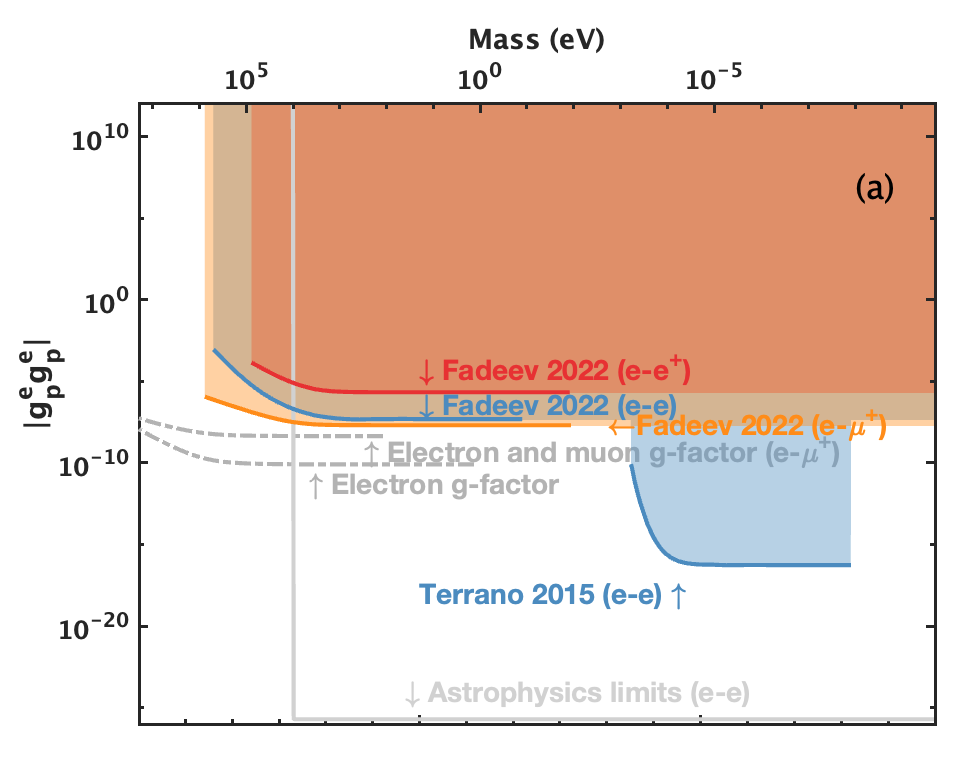
\includegraphics[width=0.48\textwidth]{Fig14_gpgp_a.eps}
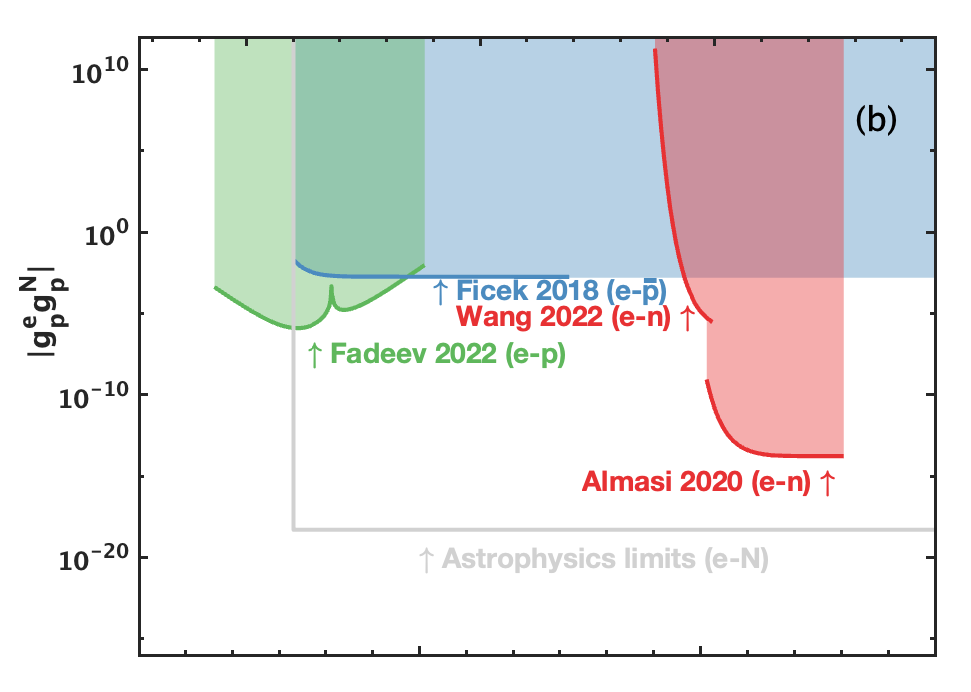
\includegraphics[width=0.48\textwidth]{Fig14_gpgp_b.eps}
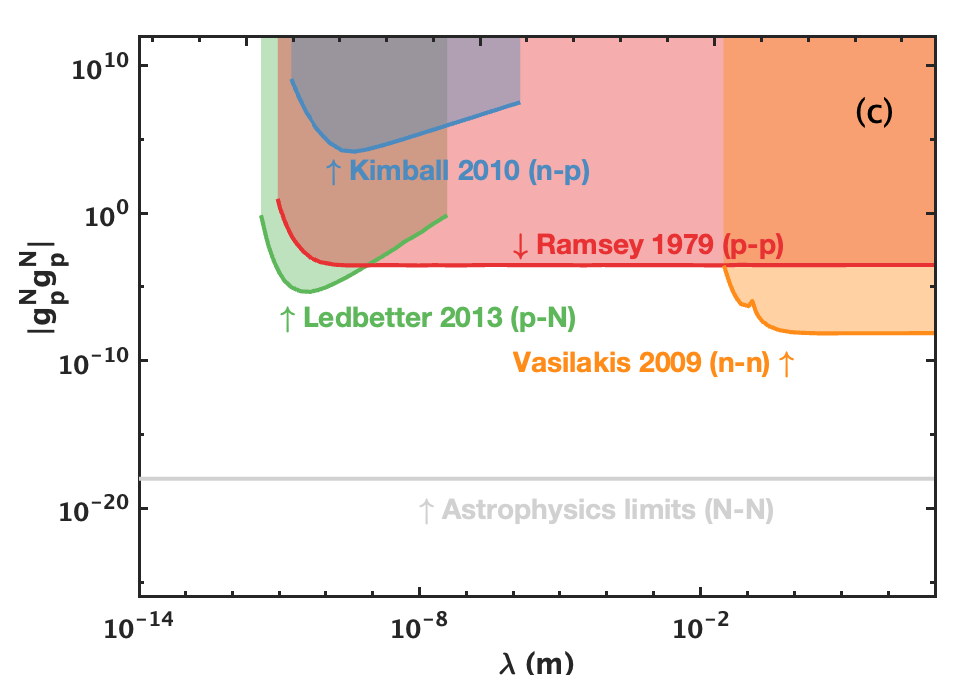
\includegraphics[width=0.48\textwidth]{Fig14_gpgp_c.eps}
\end{center}
\caption{Constraints, depicted by coloured regions, on the coupling constant product $g_p g_p$ as a function of the interaction range $\lambda$ shown on the bottom x-axis. 
The top x-axis represents the new spin-0 boson mass $M$. 
The subscript $p$ denotes the pseudoscalar coupling. 
Constraints shown for \textbf{(a)} $e$-$e$, $e$-$e^+$ and $e$-${\mu}^+$, \textbf{(b)} $e$-$n$, $e$-$p$ and $e$-$\overline{p}$, and \textbf{(c)} $n$-$n$, $n$-$p$, $p$-$p$ and $p$-$N$ couplings. 
Results are based on the $V_3$ term. 
Astrophysical bounds (light gray solid lines) and $g$-factor limits (gray dash-dotted lines) are elaborated in Appendix\,\ref{appendix_comp.}. } 
\label{gpgp-fig}
\end{figure}



%Comments for figure gpgp:
%Constraints to the coupling constant product $g_p^2$ as a function of the interaction range $\lambda$ (new vector boson mass) for $V_{3}$. The astrophysical (shallow solid line) and g-factor (dash-dotted lines) limits are present for comparision. 
%\YS{Can we add matching tick marks on the right-hand y-axis of the plots, like in the other figures in this review?}\LC{YES}
%\YS{Is it possible to change the colour of the astrophysical limits curves in all of the subfigures to light grey, for consistency with the colour scheme we use in the other results figures and also to more strongly differentiate the astrophysical bounds curves from the g-factor curves?}\LC{Done} 
 %\YS{In subfigure (a), the combined electron and muon g-factor ($e-\mu$) curve appears to starting weakening at boson masses $M \gtrsim 10^3$ eV, whereas in Figure 5 of \cite{frugiuele_current_2019}, the bound appears to start weakening at boson masses $M \gtrsim 10^6$ eV. Could we please check this?} \LC{This line was from Figure 4 of \cite{ohayon_precision_2022} [The solid black line] which is the constraint from the Muon 1S-2S measurement. }
%\YS{Which reference do we use for the electron g-factor bound curve in subfigure (a)? In Figure 4 of \cite{yan_constraining_2019}, it looks like the bound is a bit weaker than $10^{-10}$ if we use the left-hand y-axis scale, but it's unclear what the right-hand y-axis scale represents?}\LC{We were use dark gray line from Fig.4 of \cite{delaunay_probing_2017}.} 
%\YS{\citet{delaunay_probing_2017} presented bounds on spin-independent scalar couplings, but I think our current curve for $g_e$ looks correct.} 
%\LC{Latest: I have updated the two g-factor bounds based on Fig.5 and 6 from \citet{frugiuele_current_2019}.}
%\YS{Thank you, Lei. The position of the kink for the $g_e \times g_\mu$ curve now looks correct, but it seems our $g_e \times g_\mu$ curve is a bit weaker than the blue curve in Figure 6 of \citet{frugiuele_current_2019}. The $g_e$ curve (based on Figure 3, with the caption of Figure 5, of \citet{frugiuele_current_2019}) looks correct though.} \LC{Dear Zhenia, thank you for checking. The difference is because I multiplied both of their result by a factor of 4. This is because their Eq. (12) is different to us, they use spin S which is $\sigma/2$.}
%\YS{Dear Lei, I couldn't find an explicit definition of their interaction constants $g_{i,j}^\textrm{ALP}$ in their paper, but writing their Eq.~(12) in a form analogous to our Eq.~(\ref{pseudoscalar-pseudoscalar_potential}), I deduce that their interaction constants should match ours (up to an overall sign in the definition of the interaction constant), assuming the standard relation $\v{s} = \v{\sigma}/2$. Therefore, I don't think we need to multiply their constraints by a factor of 4. Could we please double-check this?} \LC{Dear Zhenia, you are right. I will correct it soon.}

%\YS{In subfigure (b), the Almasi 2020 (e-n) bound looks a bit weaker than the bound at the level $\sim 10^{-14}$ in the paper. Could we double check this? Also, shouldn't the Almasi 2020 (e-n) and Wang 2022 (e-n) curves intercept at a point? They look slightly mismatched.} \LC{yes, corrected.}
%\YS{In subfigure (c), in principle, the astrophysical limits (N-N) can be represented as a horizontal line for the entire shown mass range (if we consider our step function profile approximation, the dip in sensitivity would occur outside of the shown mass range).}\LC{done} 


%\begin{figure*} [!htbp]
%\begin{center}
%\includegraphics[width=0.48\textwidth]{gpgp_a.eps}
%\includegraphics[width=0.48\textwidth]{gpgp_b.eps}
%\includegraphics[width=0.48\textwidth]{gpgp_c.eps}
%\end{center}
%\caption{
%Constraints to the coupling constant product $g_p^2$ as a function of the interaction range $\lambda$ (new vector boson mass) for $V_{3}$.
%\YS{There are also limits on the pseudoscalar-pseudoscalar coupling for the electron-(anti)electron and electron-(anti)muon combinations from the consideration of measurements (and comparison with theoretical predictions) of $g$-factors of the electron and muon and the frequencies of various transitions in positronium and muonium presented in Figures 5 and 6 of \citet{frugiuele_current_2019} -- please note that the figures (but not captions) for Figures 3 and 5 appear to be mixed up -- also note that electron $g$-factor limits on $g_p^e g_p^e$ should in principle be the same as those in \citet{yan_constraining_2019}. \LC{We take the constraints form \cite{ohayon_precision_2022}}.}\YS{ok}
%\YS{According to Ref.~[20] of \citet{bollig_muons_2020}, the muon $g$-factor constraint is (in translated form) given by $g_p^\mu \lesssim 8 \times 10^{-4}$ for masses $\lesssim m_\mu$. \LC{We didn't add it to the figure because we do not have spin-dependent muon constraints. In the table III, there is a stronger constraints for $g_p^\mu$.} \YS{OK}
%Regarding the Arvanitaki 2014 (e-N) and (N-N) lines -- these aren't bounds, but are actually projections for suggested future experiments, so I would propose to remove these lines from the figures here. \LC{ok, will remove.} \YS{Thank you, Lei!}
%\citet{ficek_constraints_2017} gives bounds on $g_p^e g_p^e$ (\LC{considered, the result is same as \cite{fadeev_pseudovector_2022} and thus not presented.})from helium spectroscopy measurements and comparison with theory, as well as bounds on $g_A^e g_A^e$ (\LC{considered, the result included.}) and other combinations of parameters. \YS{OK}
%\citet{kotler_constraints_2015} gives bounds on $g_p^e g_p^e$ and $g_A^e g_A^e$ from positronium spectroscopy measurements and comparison with theory predictions.} \LC{The constraints for $e-e^+$ from Kotler have been considered and since \citet{fadeev_pseudovector_2022} has also considered similar results, we will mention it in the text but not plot another lines.}\YS{OK}
%} 
%\label{gpgp-fig}
%\end{figure*}



%%%%
%\subsubsection{$e$-$e$, $e$-$e^+$, $e$-$\mu^+$}
\subsubsection{\texorpdfstring{$e$-$e$, $e$-$e^+$, $e$-$\mu^+$}{e-e, e-e⁺, e-μ⁺}}
%Lepton-lepton \YS{Why do we use the subsection title "Lepton-lepton" here but not for the other types of interactions in this section?}\LC{Perhaps we can change all to Lepton-lepton? Here we have $e$-$\mu^+$, that is why I use Lepton-lepton before?} \YS{I realise now that we do something similar with ``Nucleon-nucleon'' in some (but not all) of the other subsection titles. In principle, I'm okay with either variant, but ideally we should be consistent with their usage.}}



%In the range $9\times10^{-15}<\lambda<3.29\times 10^{-4}$\,m, as shown in Figure\,\ref{gpgp-fig}(a), \citet{yan_constraining_2019} established constraints on the pseudoscalar/pseudoscalar type interaction $g_p^eg_p^e$, by conducting a study on the exotic spin-dependent interactions of electrons described by $V_{3}$.

%\LCa{Re-check as some content about \citet{yan_constraining_2019}  has been moved here from gAgA section. }
%\citet{yan_constraining_2019} used the anomalous magnetic moments and the electric dipole moments of the electron and the muon to constrain the exotic spin-dependent interactions. 


%\citet{yan_constraining_2019} analyzed the muon-EDM data and established constraints on the parity-violating monopole-dipole interaction mediated by ALPs. 
%The results are presented in Sec.\,\ref{subsec_g_Pg_S}. 
%Note that in Fig.\,\ref{gpgp-fig}, the results of \citet{yan_constraining_2019} are on the shorter-interaction-range side (heaviest new bosons); the search for even heavier bosons belongs to the high-energy physics domain \cite{butterworth_jet_2008, delannoy_probing_2013, von_buddenbrock_phenomenological_2016}.

In Fig.\,\ref{gpgp-fig}\,(a), we present various limits on couplings between an electron and other charged leptons. 

In the range $\lambda > 3 \times 10^{-4}$\,m, \citet{terrano_short-range_2015} placed limits on the electron-electron coupling $g_p^e g_p^e$ by studying the pseudoscalar/pseudoscalar spin-spin interaction using a Eöt-Wash torsion-balance probe, described in detail in Sec.\,\ref{METH1.SENS.MS}. 
%In their experimental apparatus, \citet{terrano_short-range_2015} utilized a `spin ring' as the active element of a torsion-pendulum detector, similar to the Eöt-Wash torsion-balance probes of electron-spin-dependent forces \cite{heckel_preferred-frame_2008, heckel_limits_2013} and short-distance gravity \cite{kapner_tests_2007,hoyle_submillimeter_2004}. The spin ring consists of 20 equally magnetized segments made of alternating high- (alnico) and low-spin-density (SmCo$_5$) materials. A second spin ring used for measuring $V_3$ or an unpolarized copper attractor for measuring $V_{9+10}$ is rotated below the torsion pendulum at a frequency $\omega$. The mass-density difference produces a modulated torque at $10\omega$ as the segments of the source with high spin (or mass) density pass under the high or low spin-density segments of the pendulum. The torsion pendulum and both attractors also have four cylinders both (tungsten or void) that provide gravitational calibration signals at $4\omega$. The torque on the pendulum was determined by performing a harmonic analysis of the twist angle $\theta$ as a function of the attractor angle $\phi=\omega t$, using a data-analysis procedure similar to that described in \citet{kapner_tests_2007}. The experimental setup allowed the attractors to be positioned close to the pendulum, with a separation of $4.12\,{\rm mm}$, enabling probing the $V_3$ interactions with $\lambda>3.95 \times 10^{-4}$\,m ($M \leq 500$ $\mu$eV). The resulting data were compared to those expected from $V_3$ interactions and from gravity, providing constraints for exotic electron-electron interactions. The ``pseudo-Goldstone detector'' developed by \citet{terrano_short-range_2015} searches for ultraweak interactions mediated by exotic bosons, providing a general probe for new hidden symmetries broken at high energies. 
The results of \citet{terrano_short-range_2015} surpassed the earlier results reported in \citet{pan_experimental_1992}; \citet{ni_search_1994}; \citet{bergmann_spin_1998}.

%\cite{ni_search_1994,pan_experimental_1992,bergmann_spin_1998}. 
% For V9+10
%In their work, \citet{terrano_short-range_2015} utilized an attractor with an unpolarized mass distribution to significantly improve laboratory bounds on CP-violating monopole-dipole forces in the range of $1.5 <M < 400 $ $\mu$eV by up to a factor of 1000.

In the range $\lambda > 4 \times 10^{-13}$\,m, \citet{fadeev_pseudovector_2022} set the best constraints on $g_p^eg_p^e$ and $g_p^eg_p^{e^+}$ using atomic spectroscopy methods. 
%Note, we can derive the same constraints on $g_p^eg_p^e$ from \citet{ficek_constraints_2017}. 
\citet{ficek_constraints_2017} obtained similar constraints on $g_p^e g_p^e$ as \citet{fadeev_pseudovector_2022}, while \citet{kotler_constraints_2015} set constraints on $g_p^e g_p^{e^+}$ similar to those in \citet{fadeev_pseudovector_2022}. 
For clarity, we have only presented the results from \citet{fadeev_pseudovector_2022} here. 
See Sec.\,\ref{subsec_g_Ag_A} for more details. 

In addition, \citet{fadeev_pseudovector_2022} 
set %the \sout{\textcolor{red}{only}} 
limits on the pseudoscalar/pseudoscalar coupling $g_p^e g_p^{{\mu}^+}$ between an electron and anti-muon. 
%\YS{I think there were bounds placed on $g_p^e g_p^{{\mu}^+}$ in the earlier paper \cite{frugiuele_current_2019} from comparisons of the measured and calculated ground-state hyperfine splitting interval in muonium.  Could you please check and update the text and figure accordingly?} \LC{\cite{frugiuele_current_2019} didn't study ${\mu}^+$ (?). We have included their electron and muon g factor bounds from their figure 6 in our Fig.\,\ref{gpgp-fig}\,(a).}\YS{They considered effects of intra-atomic exchange in muonium, so the $\mu$ for the muonium spectroscopy bounds there must be the (positively charged) anti-muon. I think the relevant curve is the red curve in their Figure 5 (but it's slightly confusing, since I think the captions to their Figures 3 and 5 have been mixed up \LCa{Yes, we noticed this.}- I think the best cross-check of this is Figure 4 of the later paper \cite{ohayon_precision_2022}). }\LC{So, we remove the word "only" and then here should be fine? And I will update the label for the result from \LC{\cite{frugiuele_current_2019}. }




%%%%
%\subsubsection{$e$-$n$, $e$-$p$ and $e$-$\overline{p}$}
\subsubsection{\texorpdfstring{$e$-$n$, $e$-$p$ and $e$-$\overline{p}$}{e-n, e-p and e-p̅}}

In Fig.\,\ref{gpgp-fig}\,(b), various limits on couplings between an electron and nucleons (or an anti-nucleon) are presented. 

In the interaction range $10^{-2} \, \textrm{m} < \lambda < 10$\,m, \citet{almasi_new_2020} utilized a rotatable SmCo$_5$ spin source and a Rb-$^{21}$Ne comagnetometer to establish the most stringent constraints on electron-neutron spin-dependent forces, specifically the pseudoscalar/pseudoscalar coupling $g_p^e g_p^n$. The constraints surpass the previous limits on $g_p^eg_p^n$ from \citet{wineland_search_1991}.
%The constraints surpass those of previous experiments, including direct limits on $g_p^eg_p^n$ from \citet{wineland_search_1991} and combination limits (not shown) obtained by combining the limit on $g_p^eg_p^e$ from \citet{terrano_short-range_2015} with the limit on $g_p^n g_p^n$ from \citet{vasilakis_limits_2009}. 
%\YS{I'm not sure if the statement about combination limits in the previous sentence is true or not. Based on the curves in \citet{vasilakis_limits_2009} and \citet{terrano_short-range_2015}, the combined limits look like they're at a level slightly better than $10^{-12}$, which looks comparable to or slightly better than the bound in \citet{almasi_new_2020}. Could we please double-check this?}\LC{You are right, they plot \citet{heckel_limits_2013} and \citet{vasilakis_limits_2009}. Then it is not worth to mention this. } 
More details about \citet{almasi_new_2020} can be found in Sec.\,\ref{subsec_g_Ag_A}. 

In the range $10^{-3} \, \textrm{m} < \lambda < 10^{-2}$\,m (within the classical QCD ``axion window''), \citet{wang_limits_2022} employed a spin-based amplifier (see Sec.\,\ref{METH1.SENS.AM.SMSA}) to search for axions and ALPs by measuring an exotic dipole-dipole interaction ($g_p^e g_p^n$) between polarized electron and neutron spins. 
%{\color{red}The experiment searched for anomalous nuclear-spin-dependent forces generated by optically pumped ${^3}$He nuclear spins source located approximately 50\,cm away by measuring variations in the ${^3}$He spin precession frequency, with a resolution of 18\,pHz.} 
%\YS{I'm confused by the previous sentence. Did \citet{wang_limits_2022} use $^3$He in their experiment? I thought they used polarised $^{87}$Rb electrons as the spin source and polarised $^{129}$Xe neutrons as the spin sensor. Are the distances of 50 cm and frequency resolution of 18 pHz correct here? Update: I think the previous sentence may have inadvertently referred to the work \cite{vasilakis_limits_2009}.} \LC{Seems a mistake was made here, we wrongly cut and pasted the sentence here. I removed it. Seems not necessary to put it back there. }
In this experiment, the exotic dipole-dipole interaction is between polarized $^{87}$Rb electrons in one vapor cell and polarized $^{129}$Xe neutrons in another vapor cell. 
The interaction between the source electrons in $^{87}$Rb and the polarised neutrons in $^{129}$Xe produces a pseudomagnetic field that is measured by the latter. 
%\YS{Technically, there is a pseudomagnetic field generated by both spins and felt by the complementary spin. Maybe better to say that the pseudomagnetic field is measured by one of these spins (see suggested wording above)?} \LC{Ok, thanks!}
The spin-based amplifier in the second cell utilized a mixed ensemble of spin-polarized $^{87}$Rb and $^{129}$Xe to amplify the resonant signal generated by the pseudomagnetic fields, 
%\YS{
which are modulated by changes in the electron polarisation
%} 
\cite{jiang_search_2021}. 
The $^{87}$Rb spins acted as a magnetometer \cite{jiang_magnetic_2019,jiang_interference_2020} to detect the enhanced field. 
The use of a spin-based amplifier allowed for high sensitivity in the search for pseudomagnetic fields associated with the $V_{3}$ potential term. 
%It should be noted that while both spin-based amplifiers and self-compensating comagnetometers \cite{vasilakis_limits_2009,almasi_new_2020,lee_improved_2018} utilize overlapping spin ensembles (e.g., $^{129}$Xe-$^{87}$Rb), a spin-based amplifier has a wider range of operational bias fields. 
%As such, a spin-based amplifier is well-suited for searches for new physics predicted by various theories beyond the standard model, such as ultralight ALPs.

\citet{ficek_constraints_2018} established stringent constraints on the exotic interaction between electrons and antiprotons 
%e-$\overline{p}$, respectively, 
via the $V_3$ potential using measurements and predictions of the spectrum of antiprotonic helium. 
Similar constraints have been obtained in \citet{fadeev_pseudovector_2022}. 
In addition, \citet{fadeev_pseudovector_2022} established stringent constraints on the exotic interaction between electrons and protons 
%\YS{
in the range $3.9 \times 10^{-13} \, \textrm{m} < \lambda < 1.3\times 10^{-8}$\,m using measurements and calculations of the spectrum of atomic hydrogen.
%} 
The details of these works are discussed in Sec.\,\ref{subsec_g_Ag_A}. 



%%%%
%\subsubsection{$N$-$N$}
\subsubsection{\texorpdfstring{$N$-$N$}{N-N}}

In Fig.\,\ref{gpgp-fig}\,(c), various limits on couplings between nucleons are shown. 



For the interaction range $\lambda > 3.3 \times 10^{-2}$\,m, \citet{vasilakis_limits_2009} utilized a comagnetometer (see Sec.\,\ref{METH1.SENS.AM.AC}) based on spin-polarized K and ${^3}$He atoms to search for a pseudoscalar-boson-mediated neutron-neutron interaction which takes the form of the $V_3$ potential.
\citet{vasilakis_limits_2009} obtained constraints on $g_p^n g_p^n$ that improved on the earlier ${^3}$He-$^{129}$Xe maser experiment \cite{glenday_limits_2008} by a factor of about 500 and represent the currently most stringent constraints. 
In addition, \citet{vasilakis_limits_2009} also set constraints on couplings to light vector bosons through the potential terms $V_2$ and $V_{11}$, as well as placing constraints on unparticle couplings to neutrons and couplings to Goldstone bosons associated with the spontaneous breaking of the Lorentz symmetry. 
The results for $V_{2}$ and $V_{11}$ can be found in Secs.\,\ref{subsec_g_Ag_A} and \ref{subsec_g_Ag_V}, respectively. 
%\LC{New sentence: Note, \citet{lee_laboratory_2023} reanalyzed data from \citet{vasilakis_limits_2009} to search for ultralight ALPs.}
%\YS{Suggested rewording: ``
Later on, \citet{lee_laboratory_2023} reanalyzed data from \citet{vasilakis_limits_2009} to search for ultralight ALP dark matter.
%''} 

Additionally, \citet{ramsey_tensor_1979}, \citet{jackson_kimball_constraints_2010} and \citet{ledbetter_constraints_2013} have established constraints on exotic interactions among the fermion pairs $p$-$p$, $p$-$N$ and $n$-$p$, respectively, based on the $V_3$ potential term. 
The details of those works can be found in Sec.\,\ref{subsec_g_Ag_A}. 



%%%
\subsubsection{Future perspectives}

There are many intriguing possibilities for the field of probing exotic interactions mediated by the exchange of a new pseudoscalar boson in the future. 

In the force range $\lambda > 3 \times 10^{-5}$\,m, 
%\YS{$\lambda > 2 \times 10^{-4}$\,m?}\LC{I take the 0.007 eV from the red line in Fig. 7 \citet{fadeev_ferromagnetic_2021}, so it is 2.8 $\times 10^{-5}$ m, right?} \YS{Thank you for explaining, Lei! This makes sense. I've rounded the number to 1 d.p.~for consistency.} 
\citet{fadeev_ferromagnetic_2021,vinante_surpassing_2021} propose to search for spin precession induced by the pseudoscalar-mediated dipole-dipole interaction by modulating the distance between a polarized SmCo$_{5}$ electron spin source and a levitated ferromagnetic gyroscope, which contains electron spins. The precession of the ferromagnetic gyroscope can be measured with a SQUID. 

%In the range $10^{-5} < \lambda < 10^{-3}$\,m \YS{
In the range $3\times 10^{-5} \, \textrm{m} < \lambda < 0.1$\,m,
%}, 
\citet{arvanitaki_resonantly_2014} propose the use of NMR to obtain the best sensitivity to an exotic dipole-dipole interaction between an electron and nucleons. 
The sensitivity of their proposed method is expected to be at a level that is competitive with astrophysical bounds. 
See Sec.\,\ref{subsec_g_Pg_S} for more details. 

In the range $10^{-8} \, \textrm{m} < \lambda < 10^{-4}$\,m, \citet{guo_searching_2024} propose a diamond-based vector magnetometer to probe $g_p^e g_p^N$. 
See Sec.\,\ref{subsec_g_Ag_A} for further details. 


%\YS{There's also a new proposal to use a diamond-based vector magnetometer with ensembles of nitrogen-vacancy centers along different axes in a diamond to probe $g_A^e g_A^N$ and $g_p^e g_p^N$, described in \citet{guo_searching_2024}.}\LC{It has been mentioned in the end of Sec.\,\ref{subsec_g_Ag_A}.}
%\url{https://arxiv.org/abs/2402.15042}. 





%%%%%%%%%%%%%%%%%%%%%%%%%%%%%%%%%%%%%%%%%%%%%%%%%%%%%%
                      % R6. g_sg_s
%%%%%%%%%%%%%%%%%%%%%%%%%%%%%%%%%%%%%%%%%%%%%%%%%%%%%%
%\subsection{Scalar/Scalar interaction $g_s g_s$    }
\subsection{\texorpdfstring{Scalar/Scalar interaction $g_sg_s$}{Scalar/Scalar interaction gsgs}}
\label{subsec_g_sg_s}

Experimental constraints on the scalar/scalar interaction $g_s g_s$ arise from the ${V}_1$ and $V_{4+5}$ potential terms: 

\begin{equation}
\label{gsgs_V1}
V_1|_{ss} = - g^X_s g^Y_s \frac{\hbar c}{4\pi}\frac{e^{-{r}/{\lambda}}}{r} \, ,
\end{equation}

{\small
\begin{equation}
\label{gsgs_V45}
\begin{aligned}
&V_{4+5}|_{ss}=\frac{g_s^X g_s^Y}{4} \frac{\hbar^2}{c}\left\{ \boldsymbol{\sigma}_X \cdot \left( \frac{\boldsymbol{p}_X}{m_X^2} \times \hat{\boldsymbol{r}} \right), \left( \frac{1}{r^2} + \frac{M}{r} \right) \frac{e^{-Mr}}{8 \pi} \right\} \\
&\Rightarrow g_s^X g_s^Y \frac{\hbar^2}{16\pi c}\frac{m_Y}{m_X(m_X+m_Y)} \, \boldsymbol{\sigma}_X \cdot(\boldsymbol{v} \times \hat{\boldsymbol{r}}) \left(\frac{1}{r^2}+\frac{1}{\lambda r}\right) e^{-r/\lambda} \, , 
\end{aligned}
\end{equation}
}with the expression in the second line of Eq.\,\eqref{gsgs_V45} written in the two-body C.M. frame. 
%\LC{New content: Note that these works, e.g., \citet{heckel_preferred-frame_2008}; \citet{haddock_search_2018}; \citet{kim_experimental_2018}; \citet{wu_new_2023}, which study $V_{4+5}$ but do not directly set constraints on $g_s^X g_s^Y$, can transfer their constraints to $g_s^X g_s^Y$ by comparing their equations with Eq.\,\eqref{gsgs_V45}. See more details in Tab.\,\ref{tabel_f-gg} in App.\,\ref{appendixA}.}
%\YS{OK. Suggested slight rewording: 
Note that papers, such as \citet{heckel_preferred-frame_2008}; \citet{haddock_search_2018}; \citet{kim_experimental_2018}; \citet{wu_new_2023},
which studied the $V_{4+5}$ term but did not directly set constraints on $g_s^X g_s^Y$, can transfer their constraints to $g_s^X g_s^Y$ by comparing their equations with Eq.\,\eqref{gsgs_V45}. See Tab.\,\ref{tabel_f-gg} in App.\,\ref{appendixA} for more details.
%} 


\iffalse
The modified $V_{4+5}|_{ss}$ will be, obtained similar to Eq\,\ref{gaga_V45}.
\begin{equation}\label{gsgs_V45new}
\begin{split}
\color{red}{
    &V_{4+5}|_{ss}}\\
    & \color{blue}{=\frac{g_s^X g_s^Y}{16\pi} \frac{m_Y}{m_X(m_X+m_Y)}\boldsymbol{\sigma}_X \cdot(\boldsymbol{v} \times \hat{\boldsymbol{r}}) \left (\frac{1}{r^2}+\frac{1}{\lambda r} \right ) e^{-\frac{r}{\lambda}} }\\
&\color{blue}{=g_s^Xg_s^Y \frac{\hbar^2}{16\pi c}\frac{m_Y}{m_X(m_X+m_Y)}\boldsymbol{\sigma}_X \cdot(\boldsymbol{v} \times \hat{\boldsymbol{r}}) \left( \frac{1}{r^2}+\frac{1}{\lambda r} \right ) e^{-\frac{r}{\lambda}} }\\\\
\end{split}
\end{equation}
\fi

%The $V_{4+5}$ potential describes both spin- and velocity-dependent interaction, i.e. with a hypothetical new-bosons-mediated spin and velocity-dependent interaction between a polarized spin and moving source. Recent works on $V_{4+5}$ represent a like of velocity-dependent interactions while many earlier experiments have been conducted for static spin-dependent interactions \cite{safronova_search_2018}, while spin- and velocity-dependent interactions have not been well investigated. The existing experimental constraints of $V_{4+5}$ are set by various experimental methods, covering the torsion pendulum \cite{heckel_preferred-frame_2008}, atomic magnetometers \cite{kim_experimental_2018,wu_experimental_2022}, cantilevers \cite{ding_constraints_2020}, NV center based quantum sensor \cite{chu_proposal_2022}, neutron particle physics experiment \cite{piegsa_limits_2012} and also hyperfined spectroscopy \cite{ficek_constraints_2017}, covering a wide interaction length scales.

The $V_{4+5}$ potential describes a new-boson-mediated spin- and velocity-dependent interaction between a spin and a moving source. 
While numerous earlier experiments searching for spin-dependent forces focused on static spin-dependent interactions \cite{safronova_search_2018}, recent investigations into the $V_{4+5}$ potential exhibit a noteworthy trend toward exploring the realm of spin- and velocity-dependent interactions. 
Existing experimental constraints on the $V_{4+5}$ term have been obtained using various experimental methods, including the torsion pendulum \cite{heckel_preferred-frame_2008}, atomic magnetometers \cite{kim_experimental_2018,wu_experimental_2022}, cantilevers \cite{ding_constraints_2020}, NV center-based quantum sensors \cite{chu_proposal_2022},
%neutron particle physics experiments %\YS{Maybe we could instead use the following description ?: 
neutron spin rotation experiments
%} \LC{Ok}
\cite{piegsa_limits_2012}, and atomic hyperfine spectroscopy \cite{ficek_constraints_2017}. 
These experiments cover a broad range of interaction length scales. 
%Most of the experiments study $V_{4+5}$ can also set constraints on coupling of $V_{12+13}$ interactions since the setup do not need too much modifications. 
%\LCa{ask Wei Ji to check the sentence above.} 
%\YS{Suggested slight rewording of previous sentence: 
Most of the experiments that study the $V_{4+5}$ term can also be used to study the spin- and velocity-dependent interaction $V_{12+13}$ without significant (or any) modifications to the experimental setup.
%} \LC{Ok, thanks}


Figure\,\ref{gsgs-fig} shows the current laboratory constraints on the exotic scalar/scalar interaction $g_s^X g_s^Y$ between the studied particle pairs (a) $e$-$e$, (b) $e$-$N$ and $e$-$\overline{p}$, and (c) $n$-$N$ and $p$-$N$. 
%The horizontal axes at the bottom show the range of interaction $\lambda$, inversely proportional to the mass $M$ of the boson (top axis) mediating the interaction, $\lambda=\hbar/(Mc)$. The vertical axes show the dimensionless coupling parameter $|g_sg_s|$. 
%However, according to \cite{jain_evading_2006}, there are a number of uncertainties that could affect the astrophysical bounds on $g_S^e$.
%The constraints for comparison, including those from $V_1$ limits, astrophysical limits, and combined astrophysical-$V_1$ limits, are discussed in App.\,\ref{appendix_comp.}. 
Constraints from spin-independent $V_1$ limits (dark grey dash-dotted lines), astrophysical limits (light grey solid lines) and combined astrophysical-$V_1$ limits (dotted grey line) are also shown for comparison, see Appendix~\ref{appendix_comp.} for more details. 



%%%%
\begin{figure} [!htbp]
\begin{center}
%\includegraphics[width=0.48\textwidth]{Fig14_gsgs_a.eps}
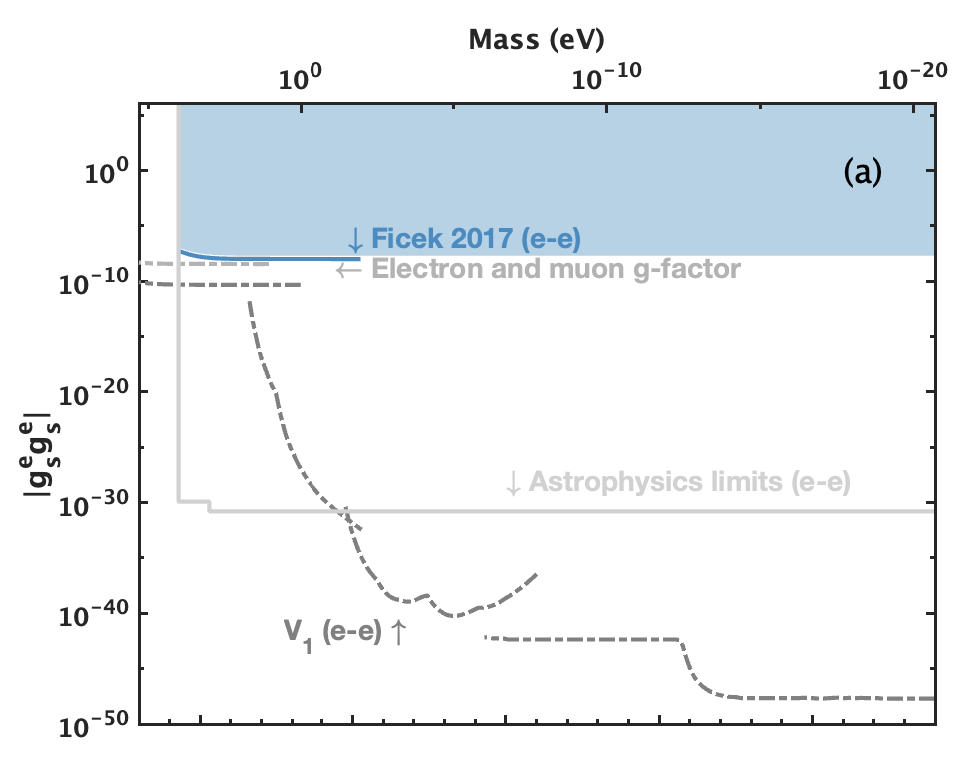
\includegraphics[width=0.48\textwidth]{Fig15_gsgs_a.eps}

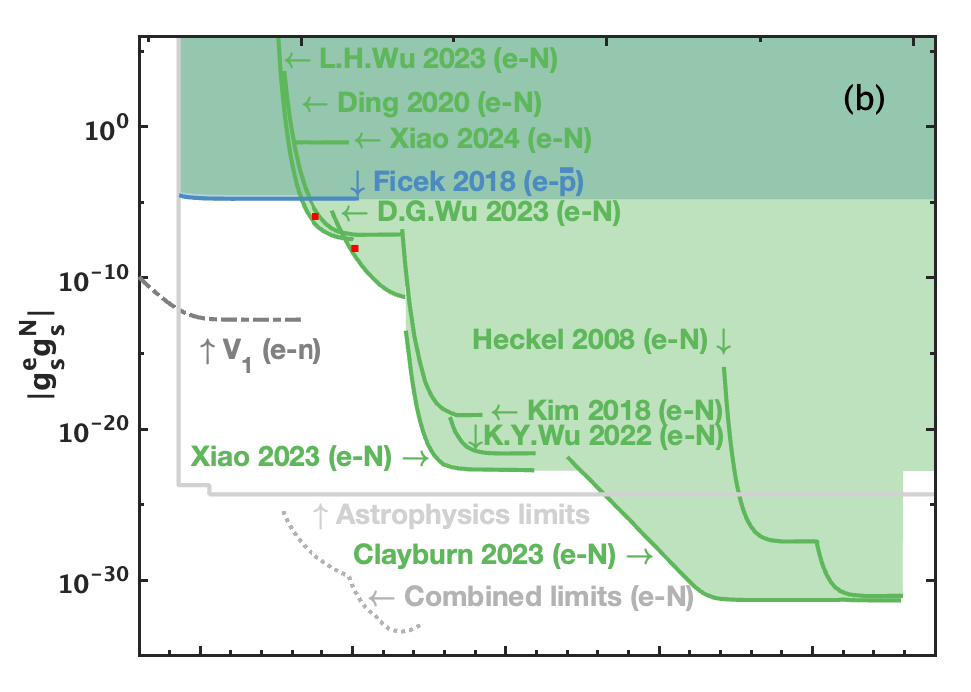
\includegraphics[width=0.48\textwidth]{Fig15_gsgs_b.eps}

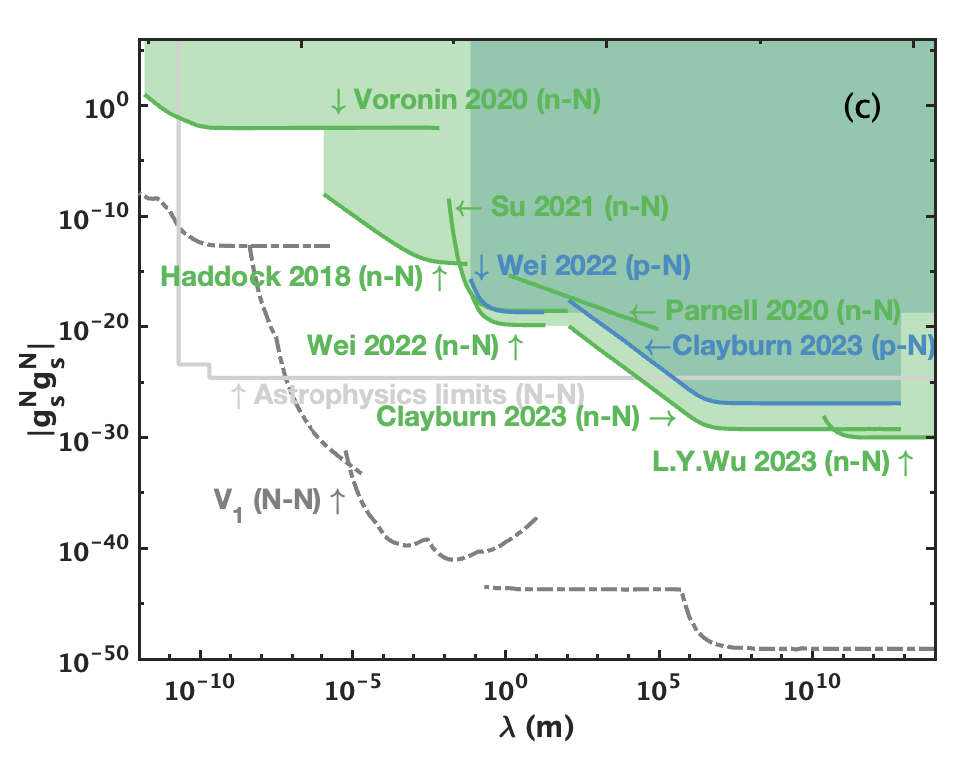
\includegraphics[width=0.48\textwidth]{Fig15_gsgs_c.eps}
\end{center}
\caption{
Constraints, depicted by coloured regions, on the coupling constant product $g_s g_s$ as a function of the interaction range $\lambda$ shown on the bottom x-axis. 
The top x-axis represents the new spin-0 boson mass $M$. 
The subscript $s$ denotes the scalar coupling. Constraints are shown for \textbf{(a)} $e$-$e$, \textbf{(b)} $e$-$N$ and $e$-$\overline{p}$, and \textbf{(c)} $n$-$N$ and $p$-$N$ couplings. 
Results are based on the $V_{4+5}$ term. 
The $V_1$ limits (dark grey dash-dotted lines), astrophysical limits (light grey solid lines) and combined astrophysical-$V_1$ limits (dotted grey line) are elaborated in Appendix~\ref{appendix_comp.}. 
%Constraints to the coupling constant product $g_s^2$ as a function of the interaction range $\lambda$ (new vector boson mass) for $V_{4+5}$.  The $V_1$ (dash-dotted line), astrophysical (shallow solid line) and combined (dotted black line) limits are present for comparision. 
In subfigure \textbf{(b)}, the two red dots represent the nonzero results from \citet{rong_observation_2020}. 
}
\label{gsgs-fig}
\end{figure}


%\LC{comments for figure gsgs}
%\LC{shaded area will be updated soon.}
%\YS{{\color{red} The ``$V_1$ (e-e)'' (and possibly also ``$V_1$ (e-n)'') curves containing $g_V^e$ may need to be updated. Please see the discussion around Eq.~(\ref{gse-alpha}).}} \lc{Done}
%\YS{Where does the ``$V_1$ (e-n)'' curve come from?} OK 
%\YS{Figure temporarily made in two-column format to fit comments.} 
%\YS{Maybe we could add a red label ``Rong 2020 (e-N)'' to the left of these two red dots in subfigure (b)?} \LC{I tried, but there are not enough space. Also, these are some ruled-out discovery. Maybe we can let the reader read the caption?} \YS{OK}
%\YS{The astrophysical limits on $g_s^e g_s^N$ in subfigure (b) look a bit strong to me. Based on our arguments in the Appendix, I would have expected a bound at the level of $g_s^e g_s^N \le [(g_s^e)^2 + (g_s^N)^2]/2 \sim 2 \times 10^{-24}$. Could we please check?} \LC{Yes, you are right.}
%\YS{In subfigure (b), is the "Combined limits (e-N)" curve a combination of the astrophysical bound on $g_s^e$ and $V_1$ laboratory bound on $g_s^N$? (If so, I would have expected a slightly stronger bound around $\labmda \sim 10^{-3}$\,m). Also, is there a reason why we don't extend this combined limits curve to higher $\lambda$ values (so that they touch/pass through the bottom x-axis) and lower $\lambda$ values?} \LC{This is a reference line used in literature, I explained it in the $g_sg_s$ subsection in App.\,\ref{appendix_comp.}} \YS{OK, I see.}
%\YS{For the "Ficek 2018 (e-$\bar{p}$)" curve in subfigure (b), do we take account of the factor $m_e/(m_e+m_{\bar{p}})$ in their definition of $V_{4+5}$ in their equation (9)? Towards the end of their paper, they mention that due to the spherical symmetry of the electron wavefunction, only the derivative over the antiproton position is relevant. I would interpret this as meaning that we should consider only the correlation $\v{\sigma}_X \cdot \v{p}_X / m_X^2$ in Eq.\,\eqref{scalar-scalar_potential}, with $X = \bar{p}$, which should give a factor of $m_e/m_\bar{p}$ suppression in our bound on $g_s^e g_s^N$ compared to their bound on $f_{4+5}^{e\bar{p}}$. Is this correct?} \LC{The factor $m_e/(m_e+m_{\bar{p}})$ and other similar one in their Eq.\,(8-10) appear because the transfer to the center of mass frame. So it maybe fine here.} \YS{OK.}
%\YS{In subfigure (b), what is the shaded green region without a solid green line below the D.G.Wu 2023 (e-N) curve? I don't see a label or explanation as to what this is.}\LC{will update soon.}
%\YS{In subfigure (b), there's a rectangular unshaded area in the bottom-right corner in the range $10^{13}<\lambda<10^{14}$m and $10^{-31}<g_s^eg_s^N<10^{-23}$. Should we fill this region with matching green colour?} \LC{we will not, \cite{clayburn_using_2023} didn't say their result is extendable.} \YS{OK}


%%%%
%\subsubsection{$e$-$e$}
\subsubsection{\texorpdfstring{$e$-$e$}{e-e}}
\citet{ficek_constraints_2017} established the only constraints so far on the spin-dependent scalar/scalar interaction $g_s g_s$ between electrons at the atomic scale through investigation of the electronic structure of $^4$He by studying the $V_{4+5}$ potential term. 
%Note that it is $V_{4}$ in the original paper, however the limit equals to the $V_{4+5}$ in their case. \LC{Ask Pasha to add an explanation here.} 
The details of this work are discussed in Sec.\,\ref{subsec_g_Ag_A}.



%%%%
%\subsubsection{$e$-$N$}
\subsubsection{\texorpdfstring{$e$-$N$}{e-N}}
\label{subsubsec:gsgs_eN}

In the range $10^{7} \, \textrm{m}<\lambda<10^{13}$\,m, \citet{heckel_preferred-frame_2008} were the first to study the exotic spin- and velocity-dependent interaction $V_{4+5}$ with their torsion-pendulum experiments (see Sec.\,\ref{METH1.SENS.MS}) and set stringent limits on the coupling $g_s^e g_s^N$. 
%\YS{I couldn't find any reference to $g_A^e g_A^N$ in \cite{heckel_preferred-frame_2008}. In Table X and Figure 15, they present bounds on the parameter $f_\perp$. They define $f_\perp$ in their equation (9) and mention that it can arise from scalar or vector boson exchange. Could we please check and update as needed?} \LC{Yes, you are right, I corrected to gsgs.}
They studied interactions between polarized electrons in the pendulum and unpolarized matter in the Earth, Moon and Sun. 
Further details on the work of \citet{heckel_preferred-frame_2008} can be found in Sec.\,\ref{subsec_g_Ag_V}. 

In the range $10^{2} \, \textrm{m} < \lambda < 10^{13}$\,m, \citet{clayburn_using_2023} utilized the results from the E\"ot-Wash torsion-pendulum experiment \cite{heckel_preferred-frame_2008} and used their own model which describes Earth as a rotating, unpolarized source \cite{hunter_using_2013, hunter_using_2014} to set the most stringent constraints on $g_s^e g_s^N$. 
%\YS{How is $g_A^e g_V^N$ related to $V_{4+5}$? At the top-right of page 4, they express $f_{4+5}$ in terms of $g_s g_s$ parameters (as well as $g_A g_A$ and $g_V g_V$), so in principle they set a bound on the scalar/scalar coupling combination.} \LC{ I corrected to gsgs.}
Further details can be found in Sec.\,\ref{subsec_g_Ag_V}. 

%For the range $4\times10^{-8}<\lambda<10$\,m,
In the interaction range $5 \times 10^{-4} \, \textrm{m} < \lambda < 10$\,m, the most stringent constraints were set by
\citet{wu_experimental_2022,kim_experimental_2018} and \citet{xiao_femtotesla_2023}. 
All of these searches used atomic magnetometers (see Sec.\,\ref{METH1.SENS.AM}) and made a noteworthy contribution by placing constraints within the classical QCD ``axion window''. 

%Around $10^{-4}<\lambda<10^{-1}$\,m 
In the range $\sim 10^{-4} \, \textrm{m} < \lambda < 10^{-1}$\,m, \citet{kim_experimental_2018} used a SERF magnetometer (see Sec.\,\ref{METH1.SENS.AM}) to study the exotic spin- and velocity-dependent interaction $V_{4+5}$ and set limits on $g_s^e g_s^N$. 
%\YS{It looks like \cite{kim_experimental_2018} set limits on the parameter $f_{4+5}$. At the top-left of page 2, they mention $V_{4+5}$ in the context of the combination of the scalar electron coupling with the scalar nucleon coupling.} \LC{corrected}
They utilized an experimental approach based on their previous proposal \cite{chu_search_2016,karaulanov_spin-exchange_2016}. 
The $^{87}$Rb magnetometer detects the pseudomagnetic field arising from the exotic interaction between polarized electrons in the Rb atoms and unpolarized nucleons of a nearby solid-state BGO mass. 

In the range $10^{-2} \, \textrm{m} < \lambda < 10$\,m, \citet{wu_experimental_2022} employed an array of magnetometers and rotationally-modulated BGO source masses to search for exotic spin-dependent interactions and improved upon the result of \citet{kim_experimental_2018} by up to a factor of 140. 
Further details on the work of \citet{wu_experimental_2022} can be found in Sec.\,\ref{subsec_g_Ag_V}.

In the range $5\times10^{-4} \, \textrm{m} < \lambda < 10$\,m, \citet{xiao_femtotesla_2023} developed a diffusion optical pumping scheme to reduce the noise and systematic errors, 
%\YS{which noise sources and systematic errors specifically?} \LC{
such as light shifts and power-broadening effects,  in a Rb magnetometer and set the most stringent constraints on $V_{4+5}$ using a rotating non-magnetic BGO crystal as the source of unpolarised nucleons. 
It is likely that their method can be applied to further improve other kinds of magnetometers. 

For interaction ranges around $\lambda \sim 10^{-6}$\,m, \citet{ding_constraints_2020} searched for the exotic spin- and velocity-dependent interaction $V_{4+5}$ by measuring the force between a gold sphere and a microfabricated magnetic structure using a cantilever-based instrument (see Sec.\,\ref{METH1.SENS.MS.MMO}) and set limits on $g_s^e g_s^N$. 
%\YS{It looks like they placed limits on the parameter $f_\perp$. Below their equation (1), they mention that $f_\perp$ may be either $g_s^e g_s^N$ or $g_V^e g_V^N$.} \LC{Yes, correc\ted}
This cantilever-based experiment, 
%\DKEdit{similarly}{ 
similar
%} 
to 
%\DKIns{
the experimental methods discussed by
%} 
\citet{leslie_prospects_2014}, \citet{chen_ultrasensitive_2021}, \citet{ren_search_2021}, and \citet{wang_proposal_2023},
%\cite{leslie_prospects_2014,ren_search_2021, wang_proposal_2023,chen_ultrasensitive_2021},
directly measures the force 
%\DKDel{[similarly to a torsion balance \citet{heckel_new_2006}]} 
between polarized electrons in a magnetic structure and unpolarized nucleons in a gold sphere,
%\DKIns{
an approach analogous to that used in torsion balance experiments such as those of \citet{heckel_new_2006}.
%}. 
A periodic magnetic structure consisting of stripes with alternating antiparallel electron spin polarization was employed to suppress spurious background signals.
In their experiments, an exotic lateral force is modulated at harmonics of the driving frequency when the magnetic structure oscillates. 
%\DKDel{\citet{ding_constraints_2020} chose to measure the sixth harmonic component, which only contains the imaginary part of the amplitude of the exotic force, and this feature enables discrimination of such exotic interactions from other forces, such as the electrostatic, Casimir and magnetic forces, which only contribute to the real part of the amplitude of the force.}
%\DK{Here it seems to me that the ``real'' and ``imaginary'' parts of the force are really referencing the components in-phase and out-of-phase with the modulation, which is physically a more intuitive explanation of the experimental signals. Maybe the last sentence could be rephrased as follows?}
%\DKIns{
\citet{ding_constraints_2020} chose to measure the sixth harmonic component, which due to the particular pattern of the magnetic structure and through the velocity-dependent exotic force is related solely to the out-of-phase component of the modulation. This feature enables discrimination of the exotic interaction from other known interactions, such as electrostatic, Casimir and magnetic forces, which in this setup do not contribute to the component of the signal at the sixth harmonic as they generate signals in phase with the modulation.
%}

%\YS{Are we talking about the 6th-harmonic component of the exotic force amplitude? Why is there only an imaginary part in this case? Don't even-harmonics contain an even number of factors of $i$, making them real? Or am I missing something?} 
%\DKDel{A periodic magnetic structure consisting of stripes with alternating antiparallel electron spin polarization was employed to further suppress spurious background signals.}
%\DK{I moved this earlier.}

%\citet{ding_constraints_2020} established laboratory constraints on the interaction between polarised electrons and unpolarised nucleons at interaction ranges $\lambda \lesssim 400\,\mu$m. 

\citet{rong_observation_2020} reported a surprising observation of a nonzero coupling between a single NV center and a mechanically oscillating SiO$_2$ mass. 
The analysis suggested the presence of a new spin- and velocity-dependent force at two interaction lengths, namely $0.38\,\mu$m, and $8.07\,\mu$m, implying the existence of two new bosons with masses of about 0.5\,eV and 25\,meV, respectively, as denoted by the two red dots in Fig.\,\ref{gsgs-fig}\,(b). 
This nonzero result has now been ruled out \cite{wu_improved_2023, wu_spin-mechanical_2023} and the authors conclude that the earlier new physics signal may have come from instrumental artifacts. 

\citet{wu_improved_2023} focused on using an ensemble-NV-diamond magnetometer to search for exotic interactions between polarized electron spins and unpolarized nucleons at the micrometer scale. 
This study utilized diamond NV centers as both polarized electron sources and sensitive sensors, and used a vibrating lead sphere as the moving unpolarised nucleon source. 
Extending the measurements to an NV ensemble rather than a single NV center, \citet{rong_observation_2020} provided better magnetic detection sensitivity. Additionally, by averaging the magnetic field sensed by each NV center, the NV ensemble is insensitive to the effect of the diamagnetism of the material of the nucleon source \cite{liang_new_2022}. 


\citet{wu_spin-mechanical_2023} demonstrated that their prototype chip, which integrates a mechanical resonator and a diamond with a single nitrogen vacancy at the microscale, sets constraints on the $V_{4+5}$ interaction that are a few orders of magnitude better compared to the sensitivity demonstrated in \citet{ding_constraints_2020}. 
Since the sensitivity improves with the number of sensors, integrating multiple sensors on a chip could significantly advance searches for exotic interactions when scaled up. 


%%%%
%\subsubsection{e-$\overline{p}$}
\subsubsection{\texorpdfstring{e-$\overline{p}$}{e-p̅}}
By comparing theoretical calculations and spectroscopic measurements of the hyperfine structure of antiprotonic helium, \citet{ficek_constraints_2018} set the only constraints on the $V_{4+5}$ potential term for the exotic semi-leptonic interaction between the fermion-antifermion pair e-$\overline{p}$. 
The details of this work are discussed in Sec.\,\ref{subsec_g_Ag_A}. 



%%%%
%\subsubsection{$N$-$N$}
\subsubsection{\texorpdfstring{$N$-$N$}{N-N}}

At astronomical distances, \citet{wu_new_2023} analyzed existing data from laboratory measurements on Lorentz and $CPT$ violation to derive upper limits on the exotic spin-dependent interaction term $V_{4+5}$. 
Details of this work are discussed in Sec.\,\ref{subsec_g_Ag_V}. 

In the interaction range $10^{2} \, \textrm{m} < \lambda < 4.5 \times 10^{10}$\,m, \citet{clayburn_using_2023} set the most stringent constraints on $g_s^n g_s^N$ (as well as for $g_s^p g_s^N$ in the range $10^{2} \, \textrm{m} < \lambda < 10^{12}$\,m). 
Further details can be found in Sec.\,\ref{subsec_g_Ag_V}. 
In the range $1 \, \textrm{m} < \lambda < 10^{5}$\,m, \citet{parnell_search_2020} set constraints on the exotic scalar-scalar interaction $g_s^n g_s^N$. 
\citet{parnell_search_2020} used a spin-echo neutron spectrometer to detect possible exotic spin-dependent interactions of neutrons influenced by Earth's gravitational field. 
An earlier 
%\DKDel{\citet*{colella_observation_1975} COW} 
experiment 
%\DKIns{
by \citet*{colella_observation_1975}
%} 
demonstrated a gravitational phase shift in neutron interferometry. 
Experiments with a neutron spin-echo interferometer \cite{de_haan_measurement_2014} further improved upon these results and \citet{parnell_search_2020} used these data to obtain strong constraints on the $V_{4+5}$ and $V_{12+13}$ interactions. These constraints have been surpassed by those obtained by \citet{su_search_2021}; \citet{wei_constraints_2022}; \citet{clayburn_using_2023}.%, with the limits presented in Fig.\,\ref{gvga-fig}\,(c). 
%\YS{I couldn't see the Parnell limits on $g_A g_V$ there. Maybe we mean to refer to Fig.\,\ref{gsgs-fig}\,(c) here?} \LC{yes, maybe we can remove this sentence.}

In the range $10^{-2} \, \textrm{m} < \lambda < 10^{2}$\,m, \citet{su_search_2021} set the constraints on $g_s^n g_s^N$ based on the spin- and velocity-dependent interaction term $V_{4+5}$. 
The details are discussed in Sec.\,\ref{subsec_g_Ag_V}. 
For interaction ranges around $\lambda \sim 1$\,m, \citet{wei_constraints_2022} conducted an experiment using a high-mass-density tungsten ring as a source and a high-energy-resolution K-Rb-$^{21}$Ne self-compensating comagnetometer. This experiment set constraints on the $V_{4+5}$ $n$-$N$ interaction and improved on the previous result of \citet{su_search_2021} by about an order of magnitude. Taking into account the fraction of proton spin in the $^{21}$Ne nucleus, this experiment also placed constraints on the $p$-$N$ interaction. 

In the range $10^{-6} \, \textrm{m} < \lambda < 10^{-2}$\,\textrm{m}, \citet{haddock_search_2018} presented a search for spin-dependent interactions between the neutron (see more in Sec.\,\ref{METH1.SENS.PBS}) and unpolarized nucleons based on the spin- and velocity-dependent interaction $V_{4+5}$, which can be interpreted as a constraint on $g_s^n g_s^N$.
%and set constraints on $g_s^n g_s^N$. 
%\YS{It looks like this work specifically considered vector bosons and placed constraints on $g_A^n g_A^N$ via the $V_{4+5}$ term ($V_5$ in their notation). The translation/reinterpretation in terms of $g_s^n g_s^N$ is done/made by us.} \LC{yes, I added a sentence under Eq.\,\eqref{gsgs_V45}. I think then it is fine to say they set constraints on $g_s^n g_s^N$.  }
%\YS{Thank you for adding the explanatory sentence in the introduction, Lei. In this case, how about slightly rephrasing the last part of the previous sentence here? ``... and set constraints on $g_s^n g_s^N$'' -> ``... , which can be interpreted as a constraint on $g_s^n g_s^N$''?} \LC{ok}
The central idea of \citet{haddock_search_2018} is that that when transversely polarized slow neutrons \cite{piegsa_limits_2012, yan_new_2013} pass near the surface of an unpolarized bulk material (copper), exotic interactions would cause the neutron polarization plane to tilt and develop a component along the neutron momentum. 
A Monte Carlo method was used to simulate the tilt induced by an exotic force. 
This experiment represents a two to four orders of magnitude improvement over the previous work \citet{piegsa_limits_2012}. 
The authors suggested that an additional two orders of magnitude improvement in sensitivity is possible by using higher intensity cold neutron beams, longer running times, and denser target materials, such as tungsten in place of copper. 
A similar experimental setup was proposed by \citet{yan_constraining_2019} to probe spin-dependent interactions of muons.

In the range $10^{-12} \, < \lambda < 10^{-6}$\,m, \citet{voronin_constraint_2020} set the best constraints on exotic $n$-$N$ interactions, 
%\YS{I think they technically constrained $g_A^n g_A^N$}
using 
neutron diffraction data in a noncentrosymmetric
crystal (see Sec.\,\ref{subsec_g_Pg_S_n-N} for more details). 

 
%\DB{The following two paragraphs belong to a general section:}
%\YS{I've drafted a new section on astrophysical phenomena (Sec.\,\ref{METH2.Astro.}) that includes the two points below.} \LC{Many thanks.}
%A general remark regarding the  comparison of the laboratory and astrophysics results is that, in contrast to astrophysics (where we do not exactly know what happens inside the starts), one may have have controlled conditions in the laboratory.     

%One should also recognize that astrophysical and laboratory constraints are typically derived at different interaction energies (momentum transfers). If the mediator is a composite particle, the laboratory and astrophysical observations cannot be compared directly.

%\LC{“Nevertheless, the laboratory experiments are still useful because they can search for interactions outside the scope of the axion-type models.” ([Wineland et al., 1991, p. 1]}
%Besides, for the range around $10^{-2}$\,m, \citet{piegsa_limits_2012} set up an experiment at the cold neutron reflectometer Narziss at the Paul Scherrer Institute and uses Ramsey's technique of separated oscillating fields to search for a pseudomagnetic neutron spin precession induced by exotic interaction between neutrons and nucleon described by the potential $V_{4+5}$. 



%%%%
\subsubsection{Future perspectives}
The recent work by \citet{rong_observation_2020},  described in Sec.\,\ref{subsubsec:gsgs_eN}, on the search for exotic forces using diamond NV centers has inspired the implementation of new measurement schemes, for example, the NV-ensemble method \cite{wu_improved_2023} and spin-mechanical quantum chips \cite{wu_spin-mechanical_2023}. 
Further improvement on the result of \citet{wu_improved_2023,wu_spin-mechanical_2023} is possible (\citealp{leslie_prospects_2014}; \citealp{chu_search_2015}, \citeyear{chu_proposal_2022}).
%\cite{leslie_prospects_2014,chu_search_2015,chu_proposal_2022}. 
\citet{chu_proposal_2022} proposed using multipulse quantum sensing protocols with NV spin ensembles to improve the sensitivity to the spin-dependent interaction $V_{4+5}$. 
The projected reach of the proposal of \citet{chu_proposal_2022} surpasses that of \citet{chu_search_2015} and \citet{leslie_prospects_2014}, which are proposals based on different techniques. 
The details of \citet{chu_proposal_2022} are introduced in Sec.\,\ref{subsec_g_Ag_V}. 


%For the range of $10<\lambda<10^{7}$\,m, it is perhaps an open opportunity for the geo-electron model method \cite{hunter_using_2013,hunter_using_2014,clayburn_using_2023}; see also \citet{zhang_search_2023}. \LCa{write the them a email.}

%\LC:{YS:If we're discussing prospective/ongoing experiments in our review, then it may be worthwhile to discuss possible muonium free-fall experiments in the context of the combination of parameters $g_s^eg_s^mu$.  See \cite{stadnik_searching_2023} and references therein. The parameters $Lambda_e$ and $\Lambda_mu$ in Figure 2 there are related to the parameters $g_s^e$ and $g_s^mu$ via the relationships $g_s^e = m_e/\Lambda_e$ and $g_s^mu = m_mu/\Lambda_mu$, respectively. }



%%%%%%%%%%%%%%%%%%%%%%%%%%%%%%%%%%%%%%%%%%%%%%%%%%%%%%
                      % R7. limit for massless boson
%%%%%%%%%%%%%%%%%%%%%%%%%%%%%%%%%%%%%%%%%%%%%%%%%%%%%%





%%%%%%%%%%%%%%%%%%%%%%%%%%%%%%%%%%%%%%%%%%%%%%%%%%%%%%
                      % Sec-Conclusions
%%%%%%%%%%%%%%%%%%%%%%%%%%%%%%%%%%%%%%%%%%%%%%%%%%%%%%

\section{Conclusion and Outlook }
\label{Sec:Sum-Out}


%%%%
\subsection*{A. Summary}
\label{Sec:Sum}

In this review, we discussed the motivation for searching for spin-dependent exotic interactions and surveyed the vast body of literature devoted to searches for such exotic interactions of various types and between various particles. 
This includes identifying relations between phenomena and experiments (such as atomic parity violation, searches for $P,T$-odd electric dipole moments, dark matter searches, and so on) that have not traditionally been directly associated with long-range exotic interaction searches. Historically, atomic PNC experiments and EDM searches have been interpreted as searches for (new) short-range forces (e.g., the usual $Z$ boson in the case of the SM or a heavy extra $Z'$ boson beyond the SM in the case of atomic PNC experiments, and a short-range/contact fermion-fermion interaction in the case of atomic EDMs). The possibility of long-range forces (on atomic scale and larger) in these types of phenomena has only been explored more recently. 

As the first step, we considered various ``catalogs'' of exotic interaction potentials and formulated the most complete and consistent set of potentials to date. 
%\YS{
We then described a broad suite of experiments of various types that can be used to probe these exotic interactions.
%} 

The strengths of exotic interactions are proportional to 
%\YS{
underlying
%} 
coupling constants, with various combinations of these generally appearing in multiple exotic potentials. 
Presenting the results of experiments and data analysis in terms of these coupling constants, as we have done here, allows for comparison of vastly different experiments, observations, and analyses in a systematic way. 
%\YS{I agree with the term ``systematic'' here, but I'm not sure the term ``universal'' is necessarily applicable.} \LC{Ok, then we can remove it.}

Following this approach, we provided a global analysis and presented exclusion limits (where possible, in the form of exclusion plots) on combinations of coupling constants, identifying the most sensitive systems and experiments, thus providing guidance for future efforts in this rapidly developing field. 

%\DB{Dear co-authors, please contemplate, what else could be added to this summary...} 

%As explained in Sec.\,\ref{Sec:Intro-Th} and \ref{Sec:formalism}, while the exotic interactions are generated by the exchange of a single boson of mass $M$, they have nine different types based on which kind of new bosons (massive vector spin 1 boson, scalar spin-0 boson, or massless vector spin-1 boson) is relevant: (1) axial-vector/vector, axial-vector/axial-vector, vector/vector, (2) pseudoscalar/scalar, pseudoscalar/pseudoscalar, scalar/scalar, (3) tensor/tensor, pseudotensor/tensor, and pseudotensor/pseudotensor interactions, as been classified in Eqs.\,(\ref{pseudovector-vector_potential})-(\ref{pseudotensor-pseudotensor_potential}). These nine interaction terms contains terms corresponding to \citet{dobrescu_spin-dependent_2006}'s $\sV_{1-16}$ in most cases. For the existing experiments, depending on whether one or both of the source and detector employ polarized particles, and if the source and detector are in relative motion, they can be sensitive to different potentials and thus belongs to one or several of the nine type interactions. While early experimental searches focused more on velocity-independent interactions, such as $V_1$, $V_2$, $V_3$, and $V_{9+10}$ (Notably, $V_{9+10}$ still attracted nearly one-third of all experimental efforts.), recent research has significantly increased efforts in exploring velocity-dependent terms, including $V_{4+5}$ and $V_{12+13}$ interactions. It is worth considering such cases because there may exist a fundamental ``microscopic'' (i.e., vertex-level) coupling that could only be detected in a velocity-dependent experiment. It may be the only access to some particular form of coupling that might go to zero in the static case.

\subsection*{B. Future directions}
\label{Sec:Conclusion_future_directions}

After a comprehensive analysis of the current state of research, one may observe that the following topics deserve attention in future studies.


%%%
\paragraph*{a. Using a unified theoretical framework.}Working within a unified theoretical framework will allow all researchers to compare their results conveniently. 
Based on the unified theoretical framework presented in Sec.\,\ref{Sec:formalism}, we underscore the imperative for future experimental studies to comprehensively explore the nine different types of interactions 
%\YS{
that generate Eqs.\,\eqref{pseudovector-vector_potential} -- \eqref{pseudotensor-pseudotensor_potential}.
%}. 
Potential terms such as $V_{2}+V_{3}$, $V_{3}$, $V_{4+5}$, $V_{9+10}$ and $V_{14q+15}$ 
%appear in multiple types of interaction \YS{
can be generated by multiple different types of interactions.
%}. 
For example, $V_{4+5}$ appears in axial-vector/axial-vector as well as vector/vector and scalar/scalar interactions. 
This unified theoretical framework overcomes the limitations of focusing solely on
%{\color{red}unphysical} \YS{I think the term ``unphysical'' isn't accurate here. Not sure what to replace it with - maybe just remove?} \LC{OK}
parameters such as $f_{4+5}$, enabling the translation of results to specific interaction types described by coupling-constant combinations, such as $g_Ag_A$, $g_Vg_V$ and $g_sg_s$, thus enabling consistent use of the full body of experimental results and comparision to results from other subfields, such as astrophysics, see Sec.\,\ref{METH2.Astro.} and App.\,\ref{appendix_comp.}. 

%this review aims to provide experimental researchers with a systematic and consistent theoretical basis for spin-dependent exotic interaction. Especially, future experimental studies $V_2$, $V_{2}+V_{3}$, $V_{4+5}$, $V_{9+10}$ and $V_{14+15}$ will not limited to one type of interaction or nonphysical parameters $f_i$, and will not be overlooking possible constraints that they can set on others type of interactions, which can make their experimental results being fully exploited. 


%%%%
\paragraph*{b. Focus on understudied potentials.} Despite the intensive study of terms like $V_{4+5}$, $V_{9+10}$, and $V_{12+13}$, %  $V_{3}$,
%\VF{$V_{12+13}$  $V_{3}$ Is this product a misprint?}\LC{yes, corrected}
a crucial term $V_3$ for both pseudoscalar/pseudoscalar and axial-vector/axial-vector interactions, in our opinion has not garnered sufficient attention, see Sec.\,\ref{subsec_g_Pg_P}. 
This gap presents an opportunity to apply advanced quantum sensors, such as NV centers and cantilevers (see Sec.\,\ref{METH1.SENS.}), in new contexts. 
%{\color{red}Additionally, while torsion pendula have been applied to explore exotic interaction between electrons, their application to $e$-$N$ remains unexplored.} 
%\YS{I'm not sure what we mean here. The torsion-pendulum-based experiment \cite{heckel_preferred-frame_2008}, e.g., did study $e$-$N$ interactions.} 
%{\color{red}The exotic interaction between $N$-$N$ has not attracted new effort for over a decade.} 
%\YS{I'm not sure what we mean here: There have been plenty of searches for exotic interactions between nucleons in recent years, presented in our summary figures. (Also, this type of comment would probably fit better in the paragraph below.)} \LC{Ok, removed}
Notably, the combination $V_{2}+V_{3}$ appearing in the vector/vector interaction (as well as tensor/tensor interaction) is an unexplored area for experimental study, as explained in Sec.\,\ref{subsec_g_Vg_V}. 

Exotic interactions between certain fermion pairs warrant more attention. 
In particular, the realm of purely leptonic (such as $e$-$e$) interactions, with the exception of the axial-vector/axial-vector couplings (see Sec.\,\ref{subsec_g_Ag_A}), appears relatively unexplored. 
Investigations of other types of interactions, such as $g_A^e g_V^e$, for the $e$-$e$ fermion pair are limited, often constrained to one or two studies for each kind of $V_i$ term. 
%\YS{Technically, $g_s^e g_s^e$ is already strongly explored and constrained via the spin-independent $V_1$ term, so the lack of searches via higher-order spin-dependent terms is perhaps not so critical. I think the second part of the sentence to some extent repeats the previous sentence. Maybe we can remove or rewrite this sentence (perhaps using a different example)?} \LC{Changed to $g_Ag_V$.} \YS{Thank you for clarifying!}
Studies of interactions involving antimatter, for example, $e$-$\overline{p}$, are particularly scarce, with only a few studies to date \citet{fadeev_pseudovector_2022,ficek_constraints_2018}. 
%When new spectroscopic transitions are measured and calculated, for example, the fine-structure anomaly in heavy muonic atoms \cite{beyer_challenging_2023}, it is possible to set new constraints on spin-dependent couplings.
%In addition, exotic interactions between the fermion pair $p$-$N$ are comparatively intensively studied for $V_{ps}$, but otherwise are rare compared to $n$-$N$ studies for other potentials. 


%%%%
\paragraph*{c. Enhancing experimental techniques.} 
The field stands to benefit significantly from advances in the sensitivity and development of new protocols in source-sensor experiments (see Sec.\,\ref{Sec:EXP.METH.1}). 
Quantum NV-diamond sensors, for example, have enabled improvements in the sensitivity to exotic interactions and promise further improvements; see, e.g., \citet{jiao_experimental_2021}; \citet{chu_proposal_2022}.
%\citet{jiao_experimental_2021, chu_proposal_2022}. 
Additionally, atom interferometry presents another promising avenue for exploration (\citealp{hamilton_atom-interferometry_2015}; \citealp{du_atom_2022}; \citealp{abe_search_2024}; \citealp{shu_constraint_2024}).
%\cite{hamilton_atom-interferometry_2015, du_atom_2022}. 
See \citet{ye_essay_2024} for more discussion of quantum sensing with atomic, molecular, and optical platforms for fundamental physics.
Levitated-magnet experiments \cite{ahrens_levitated_2024} with high sensitivity augment the tool box for exploring spin-dependent fifth forces. 


%%%%
\paragraph*{d. Attention to non-dedicated experiments.}
Besides dedicated source-sensor experiments, experiments that have not originally been designed to detect exotic spin-dependent interactions can also play an important role, especially in exploring exotic interactions on shorter length scales and between certain special fermion pairs, such as $e$-$\bar{p}$ and $e$-$\mu$. 
Constraints from such experiments are often derived by precisely comparing theory predictions and experimental results to search for a possible discrepancy which may originate from a spin-dependent exotic interaction. 
For example, EDM experiments and atomic parity-violation experiments are valuable methods worthy of further attention, see Sec.\,\ref{EXP.METH.2} for more details. 
Additionally, reinterpretation of results from studies such as those of \citet{jedi_collaboration_first_2023} could offer new insights into proton-nucleon and neutron-nucleon interactions, potentially surpassing or complementing existing constraints (\citealp{vasilakis_limits_2009}; \citealp{hunter_using_2013}).
%\cite{vasilakis_limits_2009,hunter_using_2013}. 


%%%%
\paragraph*{e. Theoretical framework expansion.}
The established theoretical framework has mainly been centered on effective Lagrangians involving spin-0 or spin-1 bosons. 
However, it is also interesting to consider possible extensions to bosons with higher spins. 
%, such as spin-2 particles like a graviton, \cite{holstein_spin_2008}. 
The study of exotic interactions mediated by massive spin-2 particles, ``heavy gravitons'', and the two-graviton exchange interaction \cite{holstein_spin_2008} may be of particular interest. 
% \VF{My comment: Effects of of ordinary graviton, long-range gravity,  are very extensively studied already! Holstein and Ross \cite{holstein_spin_2008} actually consider  two-graviton exchange and radiative corrections.}
%which we do not consider for spin 0 and 1.
%I am not sure that this reference is relevant to our review.  It may be misleading since we mean single-graviton potential. }\LC{OK, thanks, Victor. I see. 
Although these particles have not been pursued as extensively as their lower-spin counterparts, they represent a potential frontier in BSM physics. %With the rapid advancement in experimental technology and data-analysis techniques, searching for higher-spin exotic particles is becoming increasingly achievable. 
%\YS{I suppose we need to know the signatures we need to look for before said advances could help us, right?}\LC{OK. Then we can remove this statement.}
Further theoretical development, including the incorporation of two-boson exchange (\citealp{fischbach_new_1999}; \citealp{adelberger_particle-physics_2007}),
%\cite{fischbach_new_1999, adelberger_particle-physics_2007}, 
is also of paramount importance. 

In models with operators that are quadratic in the boson field, besides the simultaneous exchange of a pair of bosons between two fermions in vacuum, the exchange of a single boson between two fermions becomes possible in the presence of a background of those bosons, with the strength and range of this in-medium force potentially greatly exceeding those of two-boson exchange processes in vacuum \citet{hees_violation_2018}. 
%\DB{
Since the bosonic background can come from the ``dark sector'', e.g., in the form of dark matter, these scenarios deserve attention in future work. 
%} 
%\LC{Dear Zhenia, do you think this new sentence here is ok?} \YS{Yes, I like it.}
%\url{https://journals.aps.org/prd/abstract/10.1103/PhysRevD.98.064051}
 
% \LC{Include some of Dima's leading discussion questions (at Garching meeting) here.}




%The implications of research on spin-dependent fifth forces for our understanding of fundamental forces and the nature of the universe are potentially far-reaching. If these forces are found to exist, it would indicate that there are additional forces at play in the universe beyond the four fundamental forces that we currently know about. This could have a number of important consequences for our understanding of the fundamental laws of the universe.

%For example, the discovery of spin-dependent fifth forces could lead to new insights into the behavior of matter and the interactions between particles. These forces could provide additional information about the fundamental principles that govern the universe, and could potentially be used to help explain phenomena that are currently not well understood. This could also have implications for the development of new technologies, such as sensors and detectors that are capable of measuring these forces more accurately.

%Additionally, the discovery of spin-dependent fifth forces could have important implications for our understanding of the nature of the universe itself. If these forces are found to exist, it could provide new evidence for the existence of additional dimensions beyond the four that we currently know about. This could lead to new theories about the fundamental structure of the universe, and could potentially provide new insights into the origins and evolution of the universe.

%Overall, the research on spin-dependent fifth forces has the potential to fundamentally change our understanding of the fundamental forces and the nature of the universe. The discovery of these forces could lead to new insights into the fundamental principles that govern the universe, and could potentially have important implications for the development of new technologies and theories.

The dataset collected during preparing this review can be found here \cite{cong_fifth_2024}.

\addcontentsline{toc}{section}{Acknowledgements}
\section*{Acknowledgements}

%\textit{Acknowledgements} ---
L.~C. acknowledge helpful discussion with Younggeun Kim, Nathan Clayburn, Konstantin Gaul, Man Jiao, Protik K. Majumder, Pierre Fayet, Edoardo Vitagliano, Mario Reig Lopez, Clara Murgui Galvez \LC{and Zitong Xu}. W.~J. acknowledge helpful discussion with Dong Sheng and Yevgeny Kats.
L.~C. was partially supported by the OCPC-Helmholtz International Postdoctoral Exchange Fellowship Program (Grant No. ZD202116) and internal research funding (Stufe I) from Johannes Gutenberg University.
%F. F. is supported by the Polish National Science Centre Grant No. 2020/36/T/ST2/00323.
%V. V. F. is supported by the Australian Research Council  Grants No. DP190100974,  DP200100150 and DP230101058 and the JGU Gutenberg Research Fellowship. 
%M. G. K. is supported by RSF grant 19-12-00157 and is grateful to JGU for hospitality. 
The work of Y.~V.~S.~was supported by the Australian Research Council under the Discovery Early Career Researcher Award No. DE210101593. 
The work of D.~F.~J.~K. was supported by the U.S. National Science Foundation under grant PHYS-2110388. The work of V. V. F.  was supported by the Australian Research Council Grants No. DP230101058 and DP200100150.
F.~F.~acknowledges the support of the Austrian Science Fund (FWF), Project P 36455.
This research was supported in part by the DFG Project ID 390831469: EXC 2118 (PRISMA+ Cluster of Excellence), by the QuantERA project LEMAQUME (DFG Project No. 500314265) and by the COST Action within the project COSMIC WISPers (Grant No. CA21106), and the Munich Institute for Astro-, Particle and BioPhysics (MIAPbP), which is funded by the Deutsche Forschungsgemeinschaft (DFG, German Research Foundation) under Germany's Excellence Strategy – EXC-2094 – 390783311. 


%\newpage

%\DB{Yevgeny's comment of March 09, 2022:}

%*********************

%For the paper structure, when asking the question of which systems are most sensitive to a particular interaction(s), are you proposing to go through all of the individual interactions one by one, or group together interactions with similar features (e.g., the pseudoscalar-pseudoscalar and pseudovector-pseudovector potentials have similarities in terms of which systems are most sensitive to these potentials)? 

%I understand that the paper is devoted to spin-dependent interactions.  What is the plan for discussion of spin-independent interactions?  Some of the systems that are considered in searches for spin-dependent potentials (e.g., atomic spectroscopy) can also (simultaneously) be sensitive probes of spin-independent potentials.  Also, some potentials (e.g., the vector-vector potential) contain a spin-dependent piece as well as a (more dominant) spin-independent piece. 

%*********************



\newpage 

%%%%%%%%%%%%%%%%%%%%%%%%%%%%%%%%%%%%%%%%%%%%%%%%%%%%%%
                      % App0 
%%%%%%%%%%%%%%%%%%%%%%%%%%%%%%%%%%%%%%%%%%%%%%%%%%%%%%
\section*{Appendix} % Manually add a section titled "Appendix"

%%%%%%
\appendix 
\addcontentsline{toc}{section}{Appendix}
%%%%%%%%%%%%%%%%%%%%%%%%%%%%%%%%%%%%%%%%%%%%%%%%%%%%%%
                      % App1 
%%%%%%%%%%%%%%%%%%%%%%%%%%%%%%%%%%%%%%%%%%%%%%%%%%%%%%


%%%%
%\section{Commonly used format of $V_i$}
\section{\texorpdfstring{Commonly used format of $V_i$}{Commonly used format of Vi}}
\label{appendixA}

%\YS{I like the idea of including a table like Table\,\ref{tabel_f-gg} summarising the coefficients associated with the $\mathcal{V}_i$ potential terms. 
%In Sec.\,\ref{Sec:formalism}, we have used the $V_i$ to label for independent term or combination of the terms in Eqs.\,(\ref{pseudovector-vector_potential}) -- (\ref{pseudotensor-pseudotensor_potential}), for the purpose of map to the commomly used potentials and therefore interpreting existing experimental data sets in Sec.\,\ref{Sec:limits_main}. 

In Sec.\,\ref{Sec:formalism}, we present a complete form of the potentials, not only the leading-order terms but also the higher-order terms (e.g., $V_{4+5}$ and $V_8$) that have been studied experimentally. 
We use $V_i$ to label independent terms or combined terms to show the connection between the potentials in this review and those existing in the literature. 
To further clarify this point, here we present the potentials appearing in the main text [Eqs.\,\eqref{pseudovector-vector_potential} -- \eqref{pseudotensor-pseudotensor_potential}] as they appear in earlier references. 
For historical reasons, in contrast to the potentials in this review properly classified by the coupling-strength coefficients $g^Xg^Y$, the previous commonly used potentials are presented with the coefficients $f_i^{XY}$. 
We do the same here and then include a table (Tab.\,\ref{tabel_f-gg}) summarizing the relationship between the coefficients $f_i^{XY}$ and $g^Xg^Y$. 
In addition, we also compare the potentials in this review to the earliest ones in \citet{dobrescu_spin-dependent_2006} with an example of $V_{4+5}$, and show that we have the same result. 
In the end, we briefly point out the differences between the equations in the sections here and those in the literature. 

%This mapping to the commonly used potentials aids in interpreting existing experimental datasets, as shown in Sec.~\ref{Sec:limits_main}. 
%However, while the potentials in \citet{fadeev_revisiting_2019} and \citet{dobrescu_spin-dependent_2006} have essential same physics. 
%\YS{I'm not sure what we mean in the previous sentence.} \LCa{I have made changes.} \YS{Thank you, Lei.}
%It is not necessary and guarenteed to relate all of the potentials exactly.

%Some of the spin structures match in the case of fermions with identical masses, but not when the fermions have different masses. 
%There is also no true $\mathcal{V}_{14}$ potential term at the leading order in $q^2$, and Dobrescu doesn't have $V_{2}+V_{3}$ for the vector-vector potential. 
%Technically, what we have is a set of quasi-relations rather than true relations. 

%We first present two sets of potentials with coefficients $f_i^{XY}$ in App.\,\ref{App:f^{XY}_i}. %and then in App.\,\ref{appendix_f_gg}. 
%Then in App.\,\ref{App:appendix_f_gg_table}, we present a table giving the relationship between the coefficients $f_i^{XY}$ and pre-factors $g^Xg^Y$ in Eqs.\,\eqref{pseudovector-vector_potential} -- \eqref{pseudotensor-pseudotensor_potential}. 
%Finally, in App.\,\ref{appendix_f_gg} \YS{Which appendix?}, we give two examples of how to use Table\,\ref{tabel_f-gg} to map between the two sets of potentials. 



%\YS{I'm personally not convinced about the usefulness of presenting the numerous forms of potentials in Eqs.~(A14)-(A22). Having so many different representations looks cluttered, and it's not clear how some of these lines are related to one another; e.g., looking at the final four lines of (A22), it's not obvious if these forms are consistent with one another.} \LC{Eqs.~(A14)-(A22) will be removed.}


%%%%%%
\subsection{Potentials sorted by number}
\label{App:f^{XY}_i}

We start by presenting the set of potentials in the center-of-mass frame, following the format $V_i=f_i\sV_i$, where $\sV_i$ are the potentials from \citet{dobrescu_spin-dependent_2006} and are presented in Eqs.\,\eqref{DM_eqV1} -- \eqref{DM_eqV16}. 
For paired potentials, $\sV_{i\pm j}=\frac{1}{2}(\sV_{i}\pm\sV_{j})$. 
The first several potentials enumerated by the index $i = 1,...,8$ encompass all possible $P$-even (scalar) rotational invariants, which in the nonrelativistic limit are given by: 
%\YS{It looks like $V_{4+5}$ was missing an overall factor of $1/r$. Please check the updated formula (marked in red).}\LCa{ We are not missing $1/r$, note we use $\hat{\boldsymbol{r}}$ which is the unit of $\v r$, in Eq.(1.10) of \cite{fadeev_neue_2018}, it is $\v r$ there.}
%\YS{You're correct, Lei. I've reverted the formula. Could you please double check that we now have the original formula? I'm sorry for the false alarm.} 
\begin{equation}\label{eqV1}
V_1  = f^{XY}_1 \frac{\hbar c}{4\pi} \frac{1}{r}\,e^{-{r}/{\lambda}} \, ,
\end{equation}
\begin{equation}\label{eqV2}
V_2  = f^{XY}_2\frac{\hbar c}{4\pi}\boldsymbol{\sigma}_X\cdot\v\sigma_Y^{\,\prime}\frac{1}{r}\,e^{-{r}/{\lambda}} \, ,
\end{equation}
%\begin{equation}
%\begin{split}
\begin{align}\label{eqV3}
V_3  = f^{XY}_3 \frac{\hbar^3}{4\pi m_X^2c}\left[\boldsymbol{\sigma}_X\cdot\v\sigma_Y^{\,\prime} \left(\frac{1}{r^3}+\frac{1}{\lambda r^2}+\frac{4\pi}{3} \delta(\boldsymbol{r}) \right)\nonumber \right. \\\left. -(\boldsymbol{\sigma}_X\cdot \hat{\boldsymbol{r}})(\v\sigma_Y^{\,\prime}\cdot \hat{\boldsymbol{r}})\left(\frac{1}{\lambda^2 r}+\frac{3}{\lambda r^2}+\frac{3}{r^3}\right)\right]e^{-{r}/{\lambda}} \, ,
\end{align}
%\end{split}
%\end{equation}
\begin{equation}\label{eqV45}
V_{4+5}  = -f^{XY}_{4+5}\frac{\hbar^2}{16\pi m_X^2c} \left\{ \boldsymbol{\sigma}_X \cdot \left( \boldsymbol{p}_X \times \hat{\boldsymbol{r}} \right), \left(\frac{1}{r^2}+\frac{1}{\lambda r}\right) e^{-r/\lambda} \right\} \, , 
\end{equation}
%\begin{equation}\label{eqV67}
%\color{red}{V_{6+7}  = -f^{XY}_{6+7}\frac{\hbar}{8\pi m_X^2 c}\left\{\boldsymbol{\sigma}_X\cdot \boldsymbol{p}_X,\boldsymbol{\sigma}_Y\cdot \hat{\boldsymbol{r}}\left(\frac{1}{r^2}+\frac{1}{r\lambda}\right) e^{-{r}/{\lambda}}    \right\}} \, , 
%\end{equation}
\begin{equation}\label{eqV8}
V_{8}  = f^{XY}_8\frac{\hbar}{16\pi m_X^2 c}\left\{\boldsymbol{\sigma}_X\cdot \boldsymbol{p}_X,\left\{\v\sigma_Y^{\,\prime}\cdot \boldsymbol{p}_X, \frac{1}{r}e^{-{r}/{\lambda}}    \right\}\right\} \, . 
\end{equation}
The rest of the potentials enumerated by the index $i = 9,...,16$ encompass all possible $P$-odd (pseudoscalar) rotational invariants, given in the nonrelativistic limit by:\footnote{Note that unlike other coefficients $f_i$, the coefficient $f_{14}$ in the potential $V_{14}$
%, proportional to $\boldsymbol{\sigma}_{X}\times \boldsymbol{\sigma}_{Y} \cdot \boldsymbol{p}$, 
vanishes in the lowest order of momenta $f_i(0,0) \propto q^0$ considered by \citet{dobrescu_spin-dependent_2006}, and becomes nonzero only at order $q^2$
%the momentum transferred by the boson 
as noted in \cite{fadeev_neue_2018, fadeev_revisiting_2019}. 
This is because, while symmetries can determine the spin structure of a potential term like $V_{14}$, they do not uniquely predict the power-law dependence on the inter-particle separation (or equivalently, the momentum transfer).} 
%\YS{Should we include a minus sign (marked in red) in Eq.~(\ref{eqV1116}) for $V_{11p+16}$ for consistency? (I made some minor formatting changes in some of the equations.)} \LC{Ok, then, in Table\,\ref{tabel_f-gg}, we should remove the minus - for the value of f, right? And in Eq. A22, we should add the - too. (Thank you for make the formatting change.)} {\color{red}YS: Yes (for both). I've updated the relevant sign in Table~\ref{tabel_f-gg}.}\LC{Thank you.}
\begin{equation}\label{eqV910}
V_{9+10}=-f^{XY}_{9+10}\frac{\hbar^2}{8\pi m_X}\boldsymbol{\sigma}_X\cdot \hat{\boldsymbol{r}}\,\, \left(\frac{1}{r^2}+\frac{1}{\lambda r}\right)\, e^{-{r}/{\lambda}} \, , 
\end{equation}
\begin{equation}\label{eqV11}
V_{11}=-f^{XY}_{11}\frac{\hbar^2}{4\pi m_X} \left(\boldsymbol{\sigma}_X\times\v\sigma_Y^{\,\prime} \right) \cdot \hat{\boldsymbol{r}}\left(\frac{1}{r^2}+\frac{1}{\lambda r}\right)e^{-{r}/{\lambda}} \, ,
\end{equation}
\begin{equation}\label{eqV1213}
V_{12+13}=f^{XY}_{12+13}\frac{\hbar}{16\pi m_X} \left\{\boldsymbol{\sigma}_X \cdot \boldsymbol{p}_X, \frac{1}{r}e^{-{r}/{\lambda}}    \right\} \, , 
\end{equation}
\begin{widetext}
\begin{equation}\label{eqV1415}
\begin{aligned}
V_{14q+15} %&= \frac{g^X_p g^Y_s}{8} \left[ \left\{ \left( \v{\sigma}_X \times \v{\sigma}_Y \right) \cdot \frac{\v{p}_Y}{m_Y} , \frac{1}{r^3} + \frac{M}{r^2} + \frac{4 \pi}{3} \delta(\v{r})  \right\} -\left\{ \left( \v{\sigma}_X \cdot \hat{\v{r}} \right) \v{\sigma}_Y \cdot \left( \frac{\v{p}_Y}{m_Y} \times \hat{\v{r}} \right) , \frac{3}{r^3} + \frac{3M}{r^2} + \frac{M^2}{r}  \right\}\right]\frac{e^{-M r}}{8 \pi m_X m_Y}\\
%&=-\frac{g^X_p g^Y_s}{8} \frac{\hbar^3} {8 \pi m_X m_Y^2 c^2} \left[ \left\{ \left( \v{\sigma}_X \times \v{\sigma}_Y \right) \cdot \v{p}_X, \frac{1}{r^3} + \frac{M}{r^2} + \frac{4 \pi}{3} \delta(\v{r})  \right\} -\left\{ \left( \v{\sigma}_X \cdot \hat{\v{r}} \right) \v{\sigma}_Y \cdot \left(\v{p}_X \times \hat{\v{r}} \right) , \frac{3}{r^3} + \frac{3M}{r^2} + \frac{M^2}{r}  \right\}\right]e^{-{r}/{\lambda}} \\
%&
= f_{14q+15}^{XY} \frac{ \hbar^3} {16 \pi m_X^3 c^2} \left[ \left\{ \left( \v{\sigma}_X \times \v\sigma_Y^{\,\prime}\right) \cdot \v{p}_X, \frac{1}{r^3} + \frac{1}{\lambda r^2} + \frac{4 \pi}{3} \delta(\v{r})  \right\} -\left\{ \left( \v{\sigma}_X \cdot \hat{\v{r}} \right) \v\sigma_Y^{\,\prime}\cdot \left(\v{p}_X \times \hat{\v{r}} \right) , \frac{3}{r^3} + \frac{3}{\lambda r^2} + \frac{1}{\lambda^2 r}  \right\}\right]e^{-{r}/{\lambda}} \, , \\
\end{aligned}
\end{equation}
%with $f_{14q+15}^{XY}=-\frac{g^X_p g^Y_s}{4}\frac{m_X^2}{m_Y^2}$. 


\begin{equation}
\label{eqV1116}
\begin{aligned}
V_{11p+16}%|_{AV}%&= - \frac{g_A^X g_V^Y}{4}  \left\{ \boldsymbol{\sigma}_X \cdot \boldsymbol{p}_X , \left\{ \boldsymbol{\sigma}_Y \cdot \left[ \left( \frac{\v{p}_X}{m_X} - \frac{\v{p}_Y}{m_Y} \right) \times \hat{\v{r}} \right] , \left( \frac{1}{r^2} + \frac{M}{r} \right) \frac{e^{-M r}}{16 \pi m_X m_Y} \right\} \right\}\\
%&= - \frac{g_A^X g_V^Y}{4}  \frac{\hbar^2}{16 \pi m_X m_Y c^2} \left\{ \boldsymbol{\sigma}_X \cdot \boldsymbol{p}_X , \left\{ \boldsymbol{\sigma}_Y \cdot \left[ \left( \frac{\v{p}_X}{m_X} - \frac{\v{p}_Y}{m_Y} \right) \times \hat{\v{r}} \right] , \left( \frac{1}{r^2} + \frac{1}{\lambda r} \right)   e^{-{r}/{\lambda}}  \right\} \right\}\\
%&= - \frac{g_A^X g_V^Y}{4}  \frac{\hbar^2(m_X+m_Y)}{16 \pi (m_X m_Y)^2 c^2} \left\{ \boldsymbol{\sigma}_X \cdot \boldsymbol{p}_X , \left\{ \boldsymbol{\sigma}_Y \cdot \left( \v{p}_X \times \hat{\v{r}} \right) , \left( \frac{1}{r^2} + \frac{1}{\lambda r} \right)   e^{-{r}/{\lambda}}  \right\} \right\}\\
%&
= 
%{\color{red}-} 
-f_{11p+16}^{XY} \frac{ \hbar^2}{32 \pi m_X^3 c^2} \left\{ \boldsymbol{\sigma}_X \cdot \boldsymbol{p}_X , \left\{ \v\sigma_Y^{\,\prime} \cdot \left( \v{p}_X \times \hat{\v{r}} \right) , \left( \frac{1}{r^2} + \frac{1}{\lambda r} \right)   e^{-{r}/{\lambda}} 
  \right\} \right\} \, , \\
\end{aligned}
\end{equation}
%with $f_{11p+16}^{XY} = - \frac{g_A^X g_V^Y}{2} \frac{m_X(m_X+m_Y)}{m_Y^2}$. 
%{\small
\begin{equation}\label{eqV15}
\begin{aligned}
V_{15} = f^{XY}_{15} \frac{\hbar^3}{16\pi m_X^3 c^2} \left\{(\boldsymbol{\sigma}_X \cdot \hat{\boldsymbol{r}})[\v\sigma_Y^{\,\prime} \cdot ( \hat{\boldsymbol{r}} \times \boldsymbol{p}_X)] + (\v\sigma_Y^{\,\prime}\cdot\hat{\boldsymbol{r}}) [\boldsymbol{\sigma}_X \cdot (\hat{\boldsymbol{r}} \times \boldsymbol{p}_X)], \left(\frac{3}{r^3}+\frac{3}{\lambda r^2}+\frac{1}{\lambda^2 r}\right) e^{-{r}/{\lambda}}    \right\} %\\
\, , 
\end{aligned}
\end{equation}
%}
{\small
\begin{equation}\label{eqV16}
V_{16} = - f^{XY}_{16} \frac{\hbar^2}{32\pi m_X^3 c^2}\left[\left\{\boldsymbol{\sigma}_X\cdot\boldsymbol{p}_X, \left\{\v\sigma_Y^{\,\prime}\cdot \left( \boldsymbol{p}_X \times \hat{\boldsymbol{r}} \right), \left(\frac{1}{r^2}+\frac{1}{\lambda r}\right)\, e^{-{r}/{\lambda}}\right\}\right\}
+
\left\{\v\sigma_Y^{\,\prime}\cdot\boldsymbol{p}_X, \left\{\boldsymbol{\sigma}_X\cdot \left(\boldsymbol{p}_X \times \hat{\boldsymbol{r}}\right), \left(\frac{1}{r^2}+\frac{1}{\lambda r}\right)\,e^{-{r}/{\lambda}}\right\}\right\} 
\right] \, .
\end{equation}
}
\end{widetext}
Here, all the 
%{\color{red}labels} \YS{Do we mean 
symbols or notations
%here? Or both?} 
are defined in the same way as in the main text, see the description below Eqs.\,\eqref{pseudovector-vector_potential} -- \eqref{pseudotensor-pseudotensor_potential}. 
We also present the terms $V_{15}$ and $V_{16}$ separately [sourced from \cite{dobrescu_spin-dependent_2006,fadeev_neue_2018}], in addition to $V_{14q+15}$ and $V_{11p+16}$. While we recommend the use of $V_{14q+15}$ and $V_{11p+16}$, the former are needed to present the results of some earlier experimental works. 
%$\boldsymbol{\sigma}_{X}$ and $\boldsymbol{\sigma}_{Y}$ are vectors of Pauli matrices of the spins $\boldsymbol{s}_i=\hbar {\boldsymbol{\sigma}_i}/2$ of the two fermions, $r$ is the distance between particles $X$ and $Y$, $\hat{\boldsymbol{r}}$ is the unit position vector directed from particle $Y$ to particle $X$, $\lambda=\hbar/(Mc)$ is the reduced Compton wavelength of the new boson of mass $M$, with $\hbar$ being the reduced Plank constant and $c$ the speed of light in vacuum, and $m_X$ denotes the mass of fermion $X$. $\left\{\Box,\Box\right\}$ denotes an anticommutator. $\boldsymbol{p}$ is the momentum of fermion $X$ in the two-body centre-of-mass reference frame. 

%Here $\boldsymbol{\sigma}_{X}$ and $\boldsymbol{\sigma}_{Y}$ are vectors of Pauli matrices of the spins $\boldsymbol{s}_i=\hbar {\boldsymbol{\sigma}_i}/2$ of the two fermions. 
%$\hat{\boldsymbol{r}}$ is a unit vector pointing from particle Y to particle X. 
%$\lambda=\hbar/(Mc)$ is the reduced Compton wavelength of the new boson of mass M; $\hbar$ is the reduced Plank constant and $c$ is the speed of light in vacuum. 
%$\left\{\Box,\Box\right\}$ denotes an anticommutator. $m_X$ is the mass of fermion $X$. $\boldsymbol{p}=\boldsymbol{v}m_Xm_Y/(m_X+m_Y)$ is the momentum of fermion X in the %(atomic) 
%two-body C.M. reference frame and $\boldsymbol{v}$ is the relative velocity vector between the two particles. 
%Note that when the classical regime is relevant, momentum should be treated as a classical variable, while in the quantum treatment \cite{ficek_constraints_2017,ficek_constraints_2018}, the momentum is an operator and we substitute $\boldsymbol{p}_X=-i\hbar\boldsymbol{\nabla}_X$ and $\boldsymbol{p}_Y=-i\hbar\boldsymbol{\nabla}_Y$. 

%While many of the equations exactly the same as \citet{safronova_search_2018}, however, in some cases, there is no exact direct mapping between the two sets of potentials. 
%Most notably, the potentials in \citet{dobrescu_spin-dependent_2006} don't treat velocities (momenta) as operators and don't contain anticommutators or contact terms, and so those potentials are generally not suitable to be applied to (sub)atomic-scale phenomena. 


%%%%
\subsection{Potentials for macroscopic experiments}

Here we present the exotic potentials of Eqs.~\eqref{eqV1} -- \eqref{eqV16} with $\boldsymbol{p}_X = \boldsymbol{v} m_Xm_Y/(m_X+m_Y)$ in the %(atomic) 
two-body centre-of-mass reference frame, with $\boldsymbol{v} = \boldsymbol{v}_X - \boldsymbol{v}_Y$ being the relative velocity vector between the two particles, 
%\YS{
which we further assume to be macroscopic bodies.
%} 
Note that when the classical regime is relevant, momentum can be treated as a classical variable 
%\YS{
which commutes with the classical position vector $\v{r}$,
%}
while in the quantum treatment (\citealp{ficek_constraints_2017}; \citealp{ficek_constraints_2018}),
%\cite{ficek_constraints_2017,ficek_constraints_2018}, 
the momentum is an operator and we substitute $\boldsymbol{p}_X=-i\hbar\boldsymbol{\nabla}_X$ and $\boldsymbol{p}_Y=-i\hbar\boldsymbol{\nabla}_Y$. 
In the case of macroscopic, non-overlapping systems, we can remove the contact term $4\pi \delta(\boldsymbol{r})/3$ contained in $V_3$ 
%\YS{
and $V_{14q+15}$, which cannot extend over spatially separated regions.
%}. 
%\DB{We need an explicit explanation why we remove the delta functions for macroscopic bodies. If we have that abobe, we can just refer to that sectionn. If not, need to write it here.} \LC{The contact term describes interactions localized that could have negligible effects at a macroscopic distance.} \YS{I've elaborated a bit in the preceding sentences. Please check to see if this is okay.}\LC{Thank you!}

%\YS{I think there's an accidental duplication of the $1/r^2$ term in $V_3$ which should be removed. Please check. Also, if we're considering the macroscopic limit, then should we remove the delta function term from $V_3$?}\LC{ok, I agree.}
%with anticommutator $\left\{\Box,\Box\right\}$ calculated and $\boldsymbol{p}=\boldsymbol{v}m_Xm_Y/(m_X+m_Y)$ substituted, i.e. to be presented in the C.M. framework.
\begin{gather}
V_1  = f^{XY}_1 \frac{\hbar c}{4\pi} \frac{1}{r}\,e^{-{r}/{\lambda}} \label{eqV1f}\, ,\\
V_2  = f^{XY}_2\frac{\hbar c}{4\pi}\boldsymbol{\sigma}_X\cdot\v\sigma_Y^{\,\prime}\frac{1}{r}\,e^{-{r}/{\lambda}}\label{eqV2f} \, , \\
V_3  = f^{XY}_3 \frac{\hbar^3}{4\pi m_X^2c} \left[\boldsymbol{\sigma}_X\cdot\v\sigma_Y^{\,\prime} \left(\frac{1}{r^3}+\frac{1}{\lambda r^2}\right)\nonumber \right. \\\left.-(\boldsymbol{\sigma}_X\cdot \hat{\boldsymbol{r}})(\v\sigma_Y^{\,\prime}\cdot \hat{\boldsymbol{r}})\left(\frac{1}{\lambda^2 r}+\frac{3}{\lambda r^2}+\frac{3}{r^3}\right)  \right] e^{-{r}/{\lambda}}\label{eqV3f} \, , \\
V_{4+5} =\notag\\ -f^{XY}_{4+5} \frac{\hbar^2m_Y}{8\pi m_X(m_X+m_Y)c}\boldsymbol{\sigma}_X \cdot(\boldsymbol{v} \times \hat{\boldsymbol{r}}) \left(\frac{1}{r^2}+\frac{1}{\lambda r}\right) e^{-{r}/{\lambda}}\label{eqV45f} \, , \\
%\color{red}{V_{6+7} 
%=}\notag \\
% \color{red}{ -f^{XY}_{6+7}\frac{\hbar}{8\pi c}\frac{m_Y}{m_X(m_X+m_Y)}( \boldsymbol{\sigma}_X\cdot\boldsymbol{v})( \boldsymbol{\sigma}_Y\cdot\hat{\boldsymbol{r}})\left(\frac{1}{r^2}+\frac{1}{r\lambda}\right)e^{-{r}/{\lambda}} \label{eqV67f} \, }, \\
V_{8}  = f^{XY}_8\frac{\hbar}{4\pi c}\frac{m_Y^2}{(m_X+m_Y)^2}( \boldsymbol{\sigma}_X\cdot\boldsymbol{v})( \v\sigma_Y^{\,\prime}\cdot\boldsymbol{v})\frac{1}{r}e^{-{r}/{\lambda}} \label{eqV8f} \, , \\
%\end{gather}
%and those enumerated 9-16 encompass all possible $P$-odd (pseudoscalar) rotational invariants, given in the nonrelativistic limit by:
%\begin{gather}
V_{9+10}=-f^{XY}_{9+10}\frac{\hbar^2}{8\pi m_X}\boldsymbol{\sigma}_X\cdot \hat{\boldsymbol{r}}\,\, \left(\frac{1}{r^2}+\frac{1}{\lambda r}\right)\,\, e^{-{r}/{\lambda}} \label{eqV910f} \, , \\
V_{11}=-f^{XY}_{11}\frac{\hbar^2}{4\pi m_X} \left(\boldsymbol{\sigma}_X\times\v\sigma_Y^{\,\prime}\right) \cdot \hat{\boldsymbol{r}} \left(\frac{1}{r^2}+\frac{1}{\lambda r} \right)e^{-{r}/{\lambda}}\label{eqV11f} \, , \\
V_{12+13}=f^{XY}_{12+13}\frac{\hbar}{8\pi}\frac{m_Y}{m_X+m_Y} \boldsymbol{\sigma}_X\cdot\boldsymbol{v}\frac{1}{r}e^{-{r}/{\lambda}} \, , 
\label{eqV1213f}
\end{gather}
\begin{widetext}
\begin{gather}
%V_{14q+15}=\frac{ f_{14q+15}^{XY} m_Y^2 \hbar^3} {16 \pi m_X^2 (m_X+m_Y) c^2} \left[ \left\{ \left( \v{\sigma}_X \times \v{\sigma}_Y \right) \cdot \v{v}, \frac{1}{r^3} + \frac{M}{r^2} + \frac{4 \pi}{3} \delta(\v{r})  \right\} -\left\{ \left( \v{\sigma}_X \cdot \hat{\v{r}} \right) \v{\sigma}_Y \cdot \left(\v{v} \times \hat{\v{r}} \right) , \frac{3}{r^3} + \frac{3M}{r^2} + \frac{M^2}{r}  \right\}\right]e^{-{r}/{\lambda}}\label{eqV1415f} \, , \\
V_{14q+15} = f_{14q+15}^{XY} \frac{ m_Y \hbar^3} {8 \pi m_X^2 (m_X+m_Y) c^2} \left[ \left( \v{\sigma}_X \times \v\sigma_Y^{\,\prime}\right) \cdot \v{v} \left( \frac{1}{r^3} + \frac{1}{\lambda r^2} \right)  - \left( \v{\sigma}_X \cdot \hat{\v{r}} \right) [\v\sigma_Y^{\,\prime}\cdot \left(\v{v} \times \hat{\v{r}} \right)] \left( \frac{3}{r^3} + \frac{3}{\lambda r^2} + \frac{1}{\lambda^2 r}  \right)\right]e^{-{r}/{\lambda}}\label{eqV1415f} \, , \\
%V_{11p+16}|_{AV}= f_{11p+16}^{XY} \frac{m_Y^2 \hbar^2}{32 \pi m_X (m_X+m_Y)^2 c^2} \left\{ \boldsymbol{\sigma}_X \cdot \v{v} , \left\{ \boldsymbol{\sigma}_Y \cdot \left( \v{v} \times \hat{\v{r}} \right) , \left( \frac{1}{r^2} + \frac{1}{\lambda r} \right)   e^{-{r}/{\lambda}} \right\} \right\}\label{eqV1116f}  \, , \\
V_{11p+16}|_{AV} = - f_{11p+16}^{XY} \frac{m_Y^2 \hbar^2}{8 \pi m_X (m_X+m_Y)^2 c^2}  (\boldsymbol{\sigma}_X \cdot \v{v}) [\v\sigma_Y^{\,\prime} \cdot \left( \v{v} \times \hat{\v{r}} \right)] \left( \frac{1}{r^2} + \frac{1}{\lambda r} \right)   e^{-{r}/{\lambda}}  \label{eqV1116f}  \, , \\
V_{15}=f^{XY}_{15}\frac{\hbar^3}{8\pi m_X^2 c^2}\frac{m_Y}{(m_X+m_Y)} \left\{ (\boldsymbol{\sigma}_X \cdot \hat{\boldsymbol{r}})[\v\sigma_Y^{\,\prime} \cdot (\hat{\boldsymbol{r}} \times \boldsymbol{v})] + (\v\sigma_Y^{\,\prime}\cdot\hat{\boldsymbol{r}}) [\boldsymbol{\sigma}_X \cdot (\hat{\boldsymbol{r}} \times \boldsymbol{v})] \right\} \left(\frac{3}{r^3} + \frac{3}{\lambda r^2} + \frac{1}{\lambda^2 r}\right) e^{-{r}/{\lambda}}\label{eqV15f} \, , \\
V_{16}=-f^{XY}_{16}\frac{\hbar^2}{8\pi m_X c^2}\frac{m_Y^2}{(m_X+m_Y)^2}\left\{ (\boldsymbol{\sigma}_X\cdot\boldsymbol{v}) [\v\sigma_Y^{\,\prime} \cdot (\boldsymbol{v}\times \hat{\boldsymbol{r}})] + (\v\sigma_Y^{\,\prime}\cdot\boldsymbol{v}) [\boldsymbol{\sigma}_X \cdot (\boldsymbol{v}\times \hat{\boldsymbol{r}})] \right\} \left(\frac{1}{r^2}+\frac{1}{\lambda r}\right)\,\, e^{-{r}/{\lambda}}\label{eqV16f} \, . 
\end{gather}
\end{widetext}

%\YS{In Eq.~(\ref{eqV1415f}) above, I think the $m_Y^2$ (in red) should be $m_Y$ (marked in black to the right of it). Could we please check?} \LC{You are right, corrected.}
%\YS{Similar to my comment related to the previous set of equations above, should we include a minus sign (marked in red) in Eq.~(\ref{eqV1116f}) for $V_{11p+16}$ for consistency? }\LC{Yes} {\color{red}YS: OK, thank you for confirming. I think everything is self-consistent now.}\LC{Thank you!}




%%%%%
%\subsection{Relationship between $f_i^{XY}$ and $g^Xg^Y$}
\subsection{\texorpdfstring{Relationship between $f_i^{XY}$ and $g^Xg^Y$}{Relationship between fiXY and gXgY}}
\label{App:appendix_f_gg_table}

The details of the relationship between the sets of formulae in Eqs.~\eqref{eqV1} -- \eqref{eqV16} and Eqs.~\eqref{eqV1f} -- \eqref{eqV16f} and other formats used in the literature, especially the relationship between $f_i^{XY}$ and coupling constants $g^Xg^Y$ are presented in Tab.\,\ref{tabel_f-gg}. 
In this review, we present the formulae in a way that the coefficients $f_i^{XY}$ or $g^Xg^Y$ are dimensionless. 
So neither of them shall be divided by $\hbar c$ again while plotting, which is different from how this is done in other sources, for example, \citet{safronova_search_2018}. 
%\DB{It would be good for Derek to have a look at all statements about that review as he wrote that part...}

%\YS{What's the meaning of the superscript ``D'' in the second line of $f_3$ under the ``Coupling constants'' column? And why do we also include the first line in terms of $g_A^X g_A^Y$ there? It looks different from the second line (which is what is, e.g., in Pasha's thesis).}\LC{D means from the Dobrescu, I have removed that line now.}

%\YS{I think we might have already discussed this previously, but I don't see how we can match either Eq.~(\ref{eqV15}) or (\ref{eqV15f}) to the $V_{15}$ part of Eq.~(\ref{scalar-pseudoscalar_potential}) in the C.M. frame and macroscopic limit. The former two have the same relative sign between the two terms in the spin-tensor structure, whereas the latter has a difference in sign between the two terms. I also recall that we never came to a consensus regarding $V_{16}$ - the entry here should be consistent with the formulae in the main text (or probably removed if there's no consistent answer available). What should we do with the expressions for $V_{16}$ in Eq.~(\ref{eqV16}) and (\ref{eqV16f})?} 
%\LC{We can not, so now we may present the $V_{11p+16}$ and $V_{14q+15}$ and the define the new $f_{11p+16}$ and $f_{14q+15}$. }
%\YS{This sounds good!} 

%\YS{Update 22/02/2024: The $f_3$ coefficients quoted for $g_A^X g_A^Y$ and ${g_A^X g_A^Y}^D$, taken together, don't appear to be consistent with the relation in Eq.~(\ref{gaga_V3_coefficients_relation}).}\LC{Correctted.}

%\LC{Wei Ji is going to add a column here in the table as "Forms".}

\renewcommand\arraystretch{3}
\begin{table}\normalsize
\centering
\caption{Relationship between the sets of coefficients $f_i^{XY}$ and $g^Xg^Y$. 
%\YS{Doesn't $V_{15}$ vanish for identical fermions?}\LC{yes, it vanishs.}
} 
\renewcommand{\arraystretch}{1.8} % Adjust the line spacing here
\begin{threeparttable}
\scalebox{0.85}{
\begin{tabular}{c|c|c} %>{\columncolor{green}}
\hline
\hline
$f_i^{XY}$& Coupling constants & Fermion pairs studied\\
\hline
$f_2^{XY}$& $g_A^Xg_A^Y\times(-1)$& $e$-$e$ ($e^+$), $e$-${\mu}^+$, $e$-$n$ \\
&&$e$-$p$($\overline{p}$), $p$-$N$, $n$-$p$, $n$-$n$ \\
\hline
$f_3^{XY}$& $g_A^Xg_A^Y\times[-(\frac{c}{\hbar} m_X \lambda)^2]$ &$e$-$e$($e^+$), $e$-${\mu}^+$, $e$-$p$($\overline{p}$) \\
%&{\color{red}$(g_A^X g_A^Y)_D\times[\frac{1}{8}(1+\frac{m_X^2}{m_Y^2})]$}& \\
&$g_p^Xg_p^Y\times(-\frac{m_X}{4m_Y})$& $e$-$n$, $p$-$N(p)$, $n$-$p$, $n$-$n$ \\
&$g_V^Xg_V^Y \times\frac{m_X}{4m_Y}$&\\
\hline
$f_{4+5}^{XY}$&  $- g_A^Xg_A^Y\times( \frac{1}{2}\frac{m_X^2}{m_Y^2})$&$e$-$e$, $e$-$\overline{p}$, $e$-$N$, $p$-$N$, $n$-$N$ \\
&$- g_V^Xg_V^Y \times (\frac{1}{2}+\frac{m_X}{m_Y})$ &  \\
&\sout{$- g_s^eg_s^N\times(\frac{1}{2})$} &\\
&\LC{$- g_s^Xg_s^Y\times \frac{1}{2}$}&\\
\hline
$f_{8}^{XY}$& $g_A^Xg_A^Y\times[-\frac{1}{2}(1+\frac{2m_X}{m_Y}+\frac{m_X^2}{m_Y^2})]$& $e$-$p(\overline{p})$, $n$-$p$, $e$-$e$, $e$-$n$ \\
\hline
$f_{9+10}^{XY}$&$g^X_p g_s^Y$&$e$-$e$, $e$-$N$, $n$-$N$, $p$-$N$, $N$-$e$ \\
\hline
$f_{11}^{XY}$&$g_V^X g_A^Y\times\frac{1}{2}+g_A^X g_V^Y\times\frac{m_X}{2m_Y}$ & $e$-$e$, $e$-$n$, $e$-$p$, $n$-$p$, $n$-$n$ \\
\hline
$f_{12+13}^{XY}$&$2 g_A^X g_V^Y\times (1+\frac{m_X}{m_Y})$ &$e$-$N$, $e$-$p$, $e$-$n$, $p$-$N$, $n$-$N$\\
\hline
$f_{14q+15}^{XY}$ & $-\frac{g^X_p g^Y_s}{4}\frac{m_X^2}{m_Y^2}$ & ---\\
\hline
$f_{11p+16}^{XY}$ & $\frac{g_A^X g_V^Y}{2} \frac{m_X(m_X+m_Y)}{m_Y^2}$  & ---\\
\hline
$f_{15}^{XY}$& $g_s^X g_p^Y \times \frac{m_X}{4m_Y} + g_p^X g_s^Y \times (-\frac{m_X^2}{4m_Y^2})$ &%{\color{red}$e$-$e$,} 
$e$-$p$, $e$-$n$\\
\hline
$f_{16}^{XY}$& $(g_V^X g_A^Y - g_V^Y g_A^X) \times\frac{m_X}{4m_Y}(1+\frac{m_X}{m_Y})$ & $e$-$p$, $e$-$n$ \\
\hline
\hline
\end{tabular}
\label{tabel_f-gg}
}
%\begin{tablenotes}
%\item \textcolor{blue}{*} Here we list the fermion pairs studied in the existing literature.
%\end{tablenotes}
\end{threeparttable}
\end{table}

\subsection{Differences among various forms of the potentials appearing in the literature and their consequences}

%\DB{Explain various differences in sign and factors of two with the key references being \cite{dobrescu_spin-dependent_2006,safronova_search_2018} and this work.}

Several key references 
(\citealp{moody_new_1984}; \citealp{dobrescu_spin-dependent_2006}; \citealp{leslie_prospects_2014}; \citealp{daido_alp_2017}; \citealp{safronova_search_2018}; \citealp{fadeev_revisiting_2019})
%\cite{moody_new_1984,dobrescu_spin-dependent_2006,safronova_search_2018,fadeev_revisiting_2019,daido_alp_2017,leslie_prospects_2014}
have discussed the forms of various potentials. 

As two examples, compared to our Eqs.\,\eqref{eqV1} -- \eqref{eqV16}, \citet{dobrescu_spin-dependent_2006} present the same coefficients $f_i$. 
%\citet{safronova_search_2018} formally provide the same $f_i$ values, but {\color{red}include} \YS{are missing} \LC{perhaps not missing, but they absorb the factor into $f_i$, as they didn't provide a definition of their $f_i$?} {\color{red}Dear Lei, you're correct. For some reason, I was thinking of $\mathcal{V}_i$ rather than the $f_i$ here.} an extra factor of {\color{red}$-1/2$} \YS{Isn't it simply a factor of $1/2$ (without the minus sign)?}\LC{yes}in $f_{4+5}$, and an extra factor of $1/2$ in $f_{9+10}$, $f_{12+13}$ and $f_{15}$. \YS{What about a missing factor of $1/2$ also for $f_{15}$ as well?} \LC{yes}\LC{How about rewrite this sentence like this: \citet{safronova_search_2018} uses the coefficients $f_i$, but an extra factor of $1/2$ is absorbed in their $f_{4+5}$, $f_{9+10}$, $f_{12+13}$, and $f_{15}$. }\YS{I like your suggested new sentence. Please see some suggested slight changes in the following variant: 
\citet{safronova_search_2018} also use the coefficients $f_i$, but absorb an extra factor of $1/2$ into their coefficients $f_{4+5}$, $f_{9+10}$, $f_{12+13}$ and $f_{15}$.
%} 
In addition, Eq.\,\eqref{eqV3} contains the contact term $4\pi\delta(\boldsymbol{r})/3$, %\YS{
which is missing in \citet{dobrescu_spin-dependent_2006} and \citet{safronova_search_2018},
%}, 
and we present 
%\YS{
the new terms
%} 
$V_{14q+15}$ and $V_{11p+16}$. 

%(However, \citet{safronova_search_2018} did not cite the result from \citet{fadeev_neue_2018} correctly and therefore their Eq.\,(63) missing an factor of $1/2$. \DB{Derek should look at this} \LC{not necessarily relevant to be discussed here.})

Using different formulae can lead to confusion when comparing the results of different experiments and a deviation in the constraints that one could set. 
We advocate the use of the set of potentials given by Eqs.\,\eqref{pseudovector-vector_potential} -- \eqref{pseudotensor-pseudotensor_potential} (or the equivalent ones in Sec.\,\ref{Sec:limits_main}) and presentation of the results in terms of the combinations of the nine coupling constants, such as $g_Ag_V$, $g_Ag_A$ and so on. 
This bypasses the differences in the definitions of the potentials discussed in this subsection. 

%\LCa{need to remove some of them if we finally decide not to use.}

\subsection{Equivalence of different forms}
\label{App:appendix_f_gg}
%\section{Derivation of the equivalence of the different formulas used}\label{appendixE}
\iffalse
Here are two examples showing that the commonly used form of potentials $V_i$ with coefficient $f_i$ are equivalent to these potential forms presented in Eqs.\,(\ref{pseudovector-vector_potential}) -- (\ref{pseudotensor-pseudotensor_potential}). 
\YS{The equations below don't appear to use Eqs.\,\eqref{pseudovector-vector_potential} -- \eqref{pseudotensor-pseudotensor_potential} in their starting form. It looks like we use Eqs.\,\eqref{eqV2} -- \eqref{eqV16} and Eqs.\,\eqref{eqV2f} -- \eqref{eqV16f}. Also, the logical flow of how we go, e.g., between the second and third lines of Eq.\,\eqref{App:V_12+13_equivalence_derivation}, and similar transitions in \eqref{App:V_4+5_equivalence_derivation}, isn't clear to me. }

\begin{equation}
\begin{aligned}
\label{App:V_12+13_equivalence_derivation}
V_{12+13}\Rightarrow&f_{12+13}\frac{\hbar}{8\pi m_X}\boldsymbol{\sigma}_X\cdot \left\{ \boldsymbol{p}, \frac{1}{r}e^{-{r}/{\lambda}}    \right\}\\
\Rightarrow &f_{12+13}\frac{\hbar}{4\pi}\frac{m_Y}{m_X+m_Y} \boldsymbol{\sigma}_X\cdot\boldsymbol{v}\frac{1}{r}e^{-{r}/{\lambda}}\\ 
\Rightarrow &g_A^Xg_V^Y(1+\frac{m_X}{m_Y})\frac{m_Y}{m_X+m_Y}\frac{\hbar}{4\pi}\boldsymbol{\sigma}_X\cdot\boldsymbol{v}\frac{e^{-{r}/{\lambda}}}{r}\\
&=g_A^Xg_V^Y\frac{\hbar}{4\pi}\boldsymbol{\sigma}_X\cdot\boldsymbol{v}\frac{e^{-{r}/{\lambda}}}{r}\\
\end{aligned}
\end{equation}


\begin{widetext}
\begin{equation}
\begin{aligned}
\label{App:V_4+5_equivalence_derivation}
V_{4+5}\Rightarrow&-f_{4+5}\frac{\hbar^2}{8\pi m_X^2c}\boldsymbol{\sigma}\cdot \left\{ \boldsymbol{p} \times \vec{r}, (\frac{1}{r^3}+\frac{1}{\lambda r^2}) e^{-\frac{r}{\lambda}}    \right\}
%=-f_{4+5}\frac{\hbar^2}{8\pi m_X^2c}\boldsymbol{\sigma}\cdot \left\{ \vec{p}_1^{\,c} \times \vec{r}, (\frac{1}{r^3}+\frac{1}{\lambda r^2}) e^{-\frac{r}{\lambda}}    \right\}\\
= -f_{4+5}\frac{\hbar^2}{8\pi m_X^2c}\boldsymbol{\sigma}\cdot\left\{ \frac{m_Xm_Y}{m_X+m_Y}\boldsymbol{v}\times \vec{r}, (\frac{1}{r^3}+\frac{1}{\lambda r^2}) e^{-\frac{r}{\lambda}}    \right\}\\
&= -f_{4+5}\frac{\hbar^2m_Y}{4\pi m_X(m_X+m_Y)c}\boldsymbol{\sigma} \cdot(\boldsymbol{v} \times \hat{\boldsymbol{r}}) (\frac{1}{r^2}+\frac{1}{\lambda r}) e^{-\frac{r}{\lambda}}\\
%\approx -f_{4+5}^{eN}\frac{\hbar^2}{4\pi m_e c}\boldsymbol{\sigma} \cdot(\boldsymbol{v} \times \hat{\boldsymbol{r}}) (\frac{1}{r^2}+\frac{1}{\lambda r}) e^{-\frac{r}{\lambda}}\\ 
\Rightarrow& -g_A^Xg_A^Y (-\frac{m_X^2}{4m_Y^2})\frac{\hbar^2m_Y}{4\pi m_X(m_X+m_Y)c}\boldsymbol{\sigma} \cdot(\boldsymbol{v} \times \hat{\boldsymbol{r}}) (\frac{1}{r^2}+\frac{1}{\lambda r}) e^{-\frac{r}{\lambda}}
=g_A^Xg_A^Y \frac{m_X}{m_Y(m_X+m_Y)}\frac{\hbar^2}{16\pi c}\boldsymbol{\sigma} \cdot(\boldsymbol{v} \times \hat{\boldsymbol{r}}) (\frac{1}{r^2}+\frac{1}{\lambda r}) e^{-\frac{r}{\lambda}}\\ 
%&=-f_{4+5}^{nN}\frac{\hbar^2}{8\pi m_n c}\boldsymbol{\sigma} \cdot(\boldsymbol{v} \times \hat{\boldsymbol{r}}) (\frac{1}{r^2}+\frac{1}{\lambda r}) e^{-\frac{r}{\lambda}}
%=g_A^ng_A^N \frac{\hbar^2}{16\pi m_n c}\boldsymbol{\sigma} \cdot(\boldsymbol{v} \times \hat{\boldsymbol{r}}) (\frac{1}{r^2}+\frac{1}{\lambda r}) e^{-\frac{r}{\lambda}}\\
\Rightarrow & g_V^eg_V^N  \frac{\hbar^2}{16\pi c} \frac{2m_X+m_Y}{m_X(m_X+m_Y)}\boldsymbol{\sigma} \cdot(\boldsymbol{v} \times \hat{\boldsymbol{r}}) (\frac{1}{r^2}+\frac{1}{\lambda r}) e^{-\frac{r}{\lambda}}\\ 
\Rightarrow & g_s^eg_s^N \frac{\hbar^2m_Y}{16\pi m_X(m_X+m_Y)c}\boldsymbol{\sigma} \cdot(\boldsymbol{v} \times \hat{\boldsymbol{r}}) (\frac{1}{r^2}+\frac{1}{\lambda r}) e^{-\frac{r}{\lambda}}\\ 
\end{aligned}
\end{equation}
\end{widetext}

The relationship between the sets of coefficients $f_i^{XY}$ and $g^Xg^Y$ can be found in Tab.\,\ref{tabel_f-gg}. 
\fi

We take $V_{4+5}$ as an example to show the correspondence of the potentials from \citet{dobrescu_spin-dependent_2006} with the ones in this review. 
%\section{$V_{4+5}$}
In the derivations below, we apply the approximation $m_e \ll m_N$ for the $e$-$N$ fermion pair. 


%%%
\subsubsection*{a. $g_sg_s$}
${V}_{4+5}^\textrm{DM}$ from \citet{dobrescu_spin-dependent_2006} is given by $f_{4+5} {\sV}_{4+5}$. Starting from 
\begin{equation}
{\sV}_{4,5} =-\frac{1}{2 m_X\,r^2}
\left(\v{\sigma}_X \pm \v\sigma_Y^{\,\prime}\right) 
\cdot \left(\v v\times \hat{\v{r}} \right)  
\left(1 - r\frac{d}{dr}\right) y(r)\,,
\end{equation}
\iffalse
 ${\sV}_{4}$ and ${\sV}_{5}$ separately is:
\begin{equation}
{\sV}_{4} = -\frac{1}{2 m_X\,r^2}
\left(\v{\sigma}_X + \v\sigma_Y^{\,\prime}\right) 
\cdot \left(\v v\times \hat{\v{r}} \right)  
\left(1 - r\frac{d}{dr}\right) y(r) ~~,
\end{equation}

\begin{equation}
{\sV}_{5} = -\frac{1}{2 m_X\,r^2}
\left(\v{\sigma}_X - \v\sigma_Y^{\,\prime}\right) 
\cdot \left(\v v\times \hat{\v{r}} \right)  
\left(1 - r\frac{d}{dr}\right) y(r) ~~,
\end{equation}
\fi
%\YS{
where $y(r) = \exp(-r/\lambda)/(4\pi)$,
%} 
we have
\begin{align}
&{\sV}_{4+5} =\frac{1}{2}({\sV}_{4}+{\sV}_{5}) \\
&=  -\frac{1}{ 8\pi m_X\,r^2}
\v{\sigma}_X 
\cdot \left(\v v\times \hat{\v{r}} \right)  
\left(\frac{1}{r^2}+\frac{1}{\lambda r}\right) e^{-\frac{r}{\lambda}} \, . 
\end{align}


%Eq.\,(6.2) from \citet{dobrescu_spin-dependent_2006} paper is $f_{4,5}^{eN}(0,0)=-\frac{1}{4}\big(1\pm \frac{m_e^2}{m_N^2}\big)g_s^eg_s^N$ which gives

For the exotic interaction involving the fermion pair $e$-$N$ for $g_sg_s$, taking the coefficients $f_{4,5}^{eN}(0,0)$ from Eq.\,(6.2) of \citet{dobrescu_spin-dependent_2006},
%\begin{align}
%f_{4}^{eN}(0,0)&=-\frac{1}{4}\big(1+ \frac{m_e^2}{m_N^2}\big)g_s^eg_s^N\\
%f_{5}^{eN}(0,0)&=-\frac{1}{4}\big(1- \frac{m_e^2}{m_N^2}\big)g_s^eg_s^N
%\end{align}
we have 
\begin{align}
f_{4+5}^{eN}&=f_{4}^{eN}(0,0)+f_{5}^{eN}(0,0)=-\frac{1}{2} g_s^eg_s^N\,.
\end{align}
Therefore
\begin{align}\label{V45-ss-Dob}
{V}_{4+5}|^\textrm{DM}_{ss} &=f_{4+5}^{eN} {\sV}_{4+5} \notag\\
%&= \frac{1}{2} g_s^eg_s^N \frac{1}{ 2m\,r^2} \v{\sigma}_X \cdot \left(\v v\times \hat{\v{r}} \right)  \left(1 - r\frac{d}{dr}\right) y(r) \notag\\
&= \frac{g_s^e g_s^N}{16\pi m_e} 
\v{\sigma}_e 
\cdot \left(\v v\times \hat{\v{r}} \right)  
\left(\frac{1}{r^2}+\frac{1}{\lambda r}\right) e^{-\frac{r}{\lambda}}\,. 
\end{align}

On the other hand, 
%Eq.\,\eqref{gsgs_V45} is calculated by following \citet{fadeev_neue_2018}:
%\begin{equation}
%\begin{align}\label{V45-f-Fad}
%&V_{4+5}\notag\\
%&=-f_{4+5}\frac{\hbar^2}{8\pi m_X^2c}\boldsymbol{\sigma}\cdot \left\{ \boldsymbol{p} \times \vec{r}, (\frac{1}{r^3}+\frac{1}{\lambda r^2}) e^{-\frac{r}{\lambda}}    \right\} \notag\\
%&= -f_{4+5}\frac{\hbar^2}{8\pi m_X^2c}\boldsymbol{\sigma}\cdot \frac{2m_Xm_Y}{m_X+m_Y}\boldsymbol{v}\times \vec{r}~(\frac{1}{r^3}+\frac{1}{\lambda r^2}) e^{-\frac{r}{\lambda}} \notag \\
%&= -f_{4+5}\frac{\hbar^2m_Y}{4\pi m_X(m_X+m_Y)c}\boldsymbol{\sigma} \cdot(\boldsymbol{v} \times \hat{\boldsymbol{r}}) (\frac{1}{r^2}+\frac{1}{\lambda r}) e^{-\frac{r}{\lambda}}\,.
%\end{align}
%\end{equation}
Eq.\,\eqref{eqV45f} from this review gives $V_{4+5}$ as (using the relationship between $f_{4+5}^{XY}$ and $g_s^X g_s^Y$ presented in Tab.\,\ref{tabel_f-gg}, with $\hbar=c=1$): 
%\begin{equation}
{\small
\begin{align}\label{V45-ss-Fad}
&V_{4+5}|_{ss}\notag\\
&= \left(\frac{-g_s^e g_s^N}{2}\right) \left[ \frac{-m_N}{8\pi m_e(m_e+m_N)} \right] \boldsymbol{\sigma}_e \cdot(\boldsymbol{v} \times \hat{\boldsymbol{r}}) \left( \frac{1}{r^2}+\frac{1}{\lambda r} \right) e^{-\frac{r}{\lambda}} \notag\\ 
&\approx \frac{g_s^eg_s^N}{16\pi m_e}\boldsymbol{\sigma}_e \cdot(\boldsymbol{v} \times \hat{\boldsymbol{r}}) \left(\frac{1}{r^2}+\frac{1}{\lambda r}\right) e^{-\frac{r}{\lambda}}\,. 
\end{align}
}
%\end{equation}
Therefore, Eqs.\,\eqref{V45-ss-Dob} and \eqref{V45-ss-Fad} correspond to the same potential. 


%%%
\subsubsection*{b. $g_Ag_A$}
Similarly, for $g_Ag_A$, based on Eqs.\,(4.3)
%, {\color{red}(4.4)} 
and (5.28) of \citet{dobrescu_spin-dependent_2006}, we have 
%\YS{In principle, I think Eqs.~(4.3) and (5.28) alone are sufficient to derive this result.} \LC{yes}
%which are for linear combination of $\sV_4$ and $\sV_5$,  $f_{4+5}^{eN}=\frac{m_e^2}{2m_N^2}$, therfore
\begin{align}\label{V45-AA-Dob}
&{V}_{4+5}|^\textrm{DM}_{AA} %&=f_{4+5}^{eN} {\sV}_{4+5}\\
%&= \frac{m_e^2}{2m_N^2} g_A^eg_A^N \frac{1}{2 m_e\,r^2} \v{\sigma}_X  \cdot \left(\v v\times \hat{\v{r}} \right)   \left(1 - r\frac{d}{dr}\right) y(r) \notag\\
= \frac{g_A^e g_A^N}{16\pi} \frac{m_e}{m_N^2} 
\v{\sigma}_e 
\cdot \left(\v v\times \hat{\v{r}} \right)  
\left(\frac{1}{r^2}+\frac{1}{\lambda r}\right) e^{-\frac{r}{\lambda}}\,. 
\end{align}

Based on Eq.\,\eqref{eqV45f} and the relationship between $f_{4+5}^{XY}$ and $g_A^Xg_A^Y$ presented in Tab.\,\ref{tabel_f-gg}, we have
%{\small
\begin{equation}
\begin{aligned}\label{V45-AA-Fad}
&V_{4+5}|_{AA}\\
&=  \left(\frac{- g_A^eg_A^N }{2 } \frac{m_e^2}{m_N^2}\right) \left[ \frac{-m_N}{8\pi m_e(m_e+m_N)} \right] \boldsymbol{\sigma}_e \cdot(\boldsymbol{v} \times \hat{\boldsymbol{r}})\\ &\left(\frac{1}{r^2}+\frac{1}{\lambda r} \right) e^{-\frac{r}{\lambda}} \\ 
&\approx \frac{g_A^e g_A^N}{16\pi } \frac{m_e}{m_N^2}\boldsymbol{\sigma}_e \cdot(\boldsymbol{v} \times \hat{\boldsymbol{r}}) \left(\frac{1}{r^2}+\frac{1}{\lambda r} \right) e^{-\frac{r}{\lambda}} \, . 
\end{aligned}
\end{equation}
%}
Therefore, Eqs.\,\eqref{V45-AA-Dob} and \eqref{V45-AA-Fad} have the same form. 


\subsubsection*{c. $g_Vg_V$}
In addition, for $g_Vg_V$, based on Eqs.\,(4.3)
%, {\color{red}(4.4)} 
and (5.28) of \citet{dobrescu_spin-dependent_2006}, we have 
%\YS{In principle, I think Eqs.~(4.3) and (5.28) alone are sufficient to derive this result.}\LC{yes}
%which are for linear combination of $\sV_4$ and $\sV_5$,  $f_{4+5}^{eN}=\frac{m_e^2}{2m_N^2}$, therfore
\begin{align}\label{V45-VV-Dob}
{V}_{4+5}|^\textrm{DM}_{VV}%\notag\\ %&=f_{4+5}^{eN} {\sV}_{4+5}\\
%&= (\frac{1}{2}+\frac{m_e}{m_N}) g_V^eg_V^N \frac{1}{2 m_e\,r^2} \v{\sigma}_X \cdot \left(\v v\times \hat{\v{r}} \right)  \left(1 - r\frac{d}{dr}\right) y(r) \notag\\
&= \frac{g_V^e g_V^N}{16\pi} \frac{2m_e+m_N}{ m_em_N}
\v{\sigma}_e 
\cdot \left(\v v\times \hat{\v{r}} \right)  
\left(\frac{1}{r^2}+\frac{1}{\lambda r}\right)  e^{-\frac{r}{\lambda}} \notag\\
&\approx \frac{g_V^e g_V^N}{16\pi m_e }\boldsymbol{\sigma}_e \cdot(\boldsymbol{v} \times \hat{\boldsymbol{r}}) \left(\frac{1}{r^2}+\frac{1}{\lambda r}\right) e^{-\frac{r}{\lambda}}\, . 
\end{align}

Based on Eq.\,\eqref{eqV45f} and the relationship between $f_{4+5}^{XY}$ and $g_V^Xg_V^Y$ presented in Tab.\,\ref{tabel_f-gg}, we have
{\small
\begin{align}\label{V45-VV-Fad}
&V_{4+5}|_{VV}\notag\\
&= \left[ -\frac{g_V^e g_V^N}{2} \left( \frac{2m_e + m_N}{m_N} \right) \right] \left[ \frac{-m_N}{8\pi m_e(m_e+m_N)} \right]  \boldsymbol{\sigma}_e \cdot(\boldsymbol{v} \times \hat{\boldsymbol{r}}) \notag\\
&\left(\frac{1}{r^2}+\frac{1}{\lambda r}\right) e^{-\frac{r}{\lambda}}\notag\\
&\approx \frac{g_V^e g_V^N}{16\pi m_e }\boldsymbol{\sigma}_e \cdot(\boldsymbol{v} \times \hat{\boldsymbol{r}}) \left(\frac{1}{r^2}+\frac{1}{\lambda r}\right) e^{-\frac{r}{\lambda}} \, . 
\end{align}
}

Therefore, Eqs.\,\eqref{V45-VV-Dob} and \eqref{V45-VV-Fad} correspond to the same potential. 


%Therefore, the above two equations are very similar to Eq.\ref{V45-ss-Dob} and \ref{V45-AA-Dob}, besides of a factor $-1/2$ for $V_{4+5}|_{AA}^{eN}$.
%In addition, the above three ${V}_{4+5}|_{ss,AA,VV}$ are the same as we presented in Sec.\,\ref{Sec:limits_main}, i.e. Eq.\,\eqref{gsgs_V45}, \eqref{gaga_V45} and \eqref{gvgv_V45new}.


\iffalse
\newpage
\newpage
\newpage

Below is for reference:
\begin{equation}
\begin{aligned}
V_{12+13}&=f_{12+13}\frac{\hbar}{8\pi m_X}\boldsymbol{\sigma}_X\cdot \left\{ \boldsymbol{p}, \frac{1}{r}e^{-{r}/{\lambda}}    \right\}\\
&=f_{12+13}\frac{\hbar}{4\pi}\frac{m_Y}{m_X+m_Y} \boldsymbol{\sigma}_X\cdot\boldsymbol{v}\frac{1}{r}e^{-{r}/{\lambda}}\\ 
\end{aligned}
\end{equation}
which means
\begin{equation}
\begin{aligned}
V_{12+13}^{eN}&=f_{12+13}^{eN}\frac{\hbar}{4\pi}\boldsymbol{\sigma}_X\cdot\boldsymbol{v}\frac{e^{-{r}/{\lambda}}}{r}\\
&=g_A^eg_V^N(1+\frac{m_e}{m_N})\frac{m_Y}{m_X+m_Y}\frac{\hbar}{4\pi}\boldsymbol{\sigma}_X\cdot\boldsymbol{v}\frac{e^{-{r}/{\lambda}}}{r}\\
&=g_A^eg_V^N\frac{\hbar}{4\pi}\boldsymbol{\sigma}_X\cdot\boldsymbol{v}\frac{e^{-{r}/{\lambda}}}{r}\\
\end{aligned}
\end{equation}
where the relationship $f_{12+13}^{eN}=g_A^eg_V^N(1+\frac{m_e}{m_N})$ is from Eq. (2.512) in \citet{fadeev_neue_2018}.
and
\begin{equation}
\begin{aligned}
V_{12+13}^{nN}&=f_{12+13}^{nN}\frac{\hbar}{4\pi}\boldsymbol{\sigma}_X\cdot\boldsymbol{v}\frac{e^{-{r}/{\lambda}}}{r}\\
&=g_A^ng_V^N(1+\frac{m_n}{m_N})\frac{m_Y}{m_X+m_Y}\frac{\hbar}{4\pi}\boldsymbol{\sigma}_X\cdot\boldsymbol{v}\frac{e^{-{r}/{\lambda}}}{r}\\
&=g_A^ng_V^N\frac{\hbar}{4\pi}\boldsymbol{\sigma}_X\cdot\boldsymbol{v}\frac{e^{-{r}/{\lambda}}}{r}\\
\end{aligned}
\end{equation}


\newpage
\begin{equation}
\begin{aligned}
V_{2}&=f_{2}\frac{\hbar c}{4\pi}\boldsymbol{\sigma}_X\cdot\v\sigma_Y^{\,\prime}\frac{1}{r}\,e^{-{r}/{\lambda}}\\
&=g_A^eg_A^N (-1)\frac{\hbar c}{4\pi}\boldsymbol{\sigma}_X\cdot\v\sigma_Y^{\,\prime}\frac{1}{r}\,e^{-{r}/{\lambda}}\\
&=-g_A^eg_A^N \frac{\hbar c}{4\pi}\boldsymbol{\sigma}_X\cdot\v\sigma_Y^{\,\prime}\frac{1}{r}\,e^{-{r}/{\lambda}}\\
\end{aligned}
\end{equation}

\begin{widetext}
\begin{equation}
\begin{aligned}
V_{3}&=f_{3}\frac{\hbar^3}{4\pi m_X^2c}\left[\boldsymbol{\sigma}_X\cdot\v\sigma_Y^{\,\prime}\cdot \left(\frac{1}{r^3}+\frac{1}{\lambda r^2}+\frac{4\pi}{3}\delta(r)^3\right)-(\boldsymbol{\sigma}_X\cdot \hat{\boldsymbol{r}})(\v\sigma_Y^{\,\prime}\cdot \hat{\boldsymbol{r}})\left(\frac{1}{\lambda^2 r}+\frac{3}{\lambda r^2}+\frac{3}{r^3}\right)\right]e^{-{r}/{\lambda}}\\
&=g_p^eg_p^N (-\frac{m_e}{4m_N})\frac{\hbar^3}{4\pi m_e^2c}\left[\boldsymbol{\sigma}_X\cdot\v\sigma_Y^{\,\prime}\cdot \left(\frac{1}{r^3}+\frac{1}{\lambda r^2}+\frac{4\pi}{3}\delta(r)^3\right)-(\boldsymbol{\sigma}_X\cdot \hat{\boldsymbol{r}})(\v\sigma_Y^{\,\prime}\cdot \hat{\boldsymbol{r}})\left(\frac{1}{\lambda^2 r}+\frac{3}{\lambda r^2}+\frac{3}{r^3}\right)\right]e^{-{r}/{\lambda}}\\
&=g_V^eg_V^N (\frac{m_e}{4m_N})\frac{\hbar^3}{4\pi m_e^2c}\left[\boldsymbol{\sigma}_X\cdot\v\sigma_Y^{\,\prime}\cdot \left(\frac{1}{r^3}+\frac{1}{\lambda r^2}+\frac{4\pi}{3}\delta(r)^3\right)-(\boldsymbol{\sigma}_X\cdot \hat{\boldsymbol{r}})(\v\sigma_Y^{\,\prime}\cdot \hat{\boldsymbol{r}})\left(\frac{1}{\lambda^2 r}+\frac{3}{\lambda r^2}+\frac{3}{r^3}\right)\right]e^{-{r}/{\lambda}}\\
&=g_A^eg_A^N \frac{1}{8}(1+\frac{m_e^2}{m_N^2})\frac{\hbar^3}{4\pi m_e^2c}\left[\boldsymbol{\sigma}_X\cdot\v\sigma_Y^{\,\prime}\cdot \left(\frac{1}{r^3}+\frac{1}{\lambda r^2}+\frac{4\pi}{3}\delta(r)^3\right)-(\boldsymbol{\sigma}_X\cdot \hat{\boldsymbol{r}})(\v\sigma_Y^{\,\prime}\cdot \hat{\boldsymbol{r}})\left(\frac{1}{\lambda^2 r}+\frac{3}{\lambda r^2}+\frac{3}{r^3}\right)\right]e^{-{r}/{\lambda}}\\
\end{aligned}
\end{equation}
\end{widetext}
\fi


\iffalse
\begin{equation}
\begin{aligned}
V_{6+7}&=-f_{6+7}\frac{\hbar}{8\pi {m_X}^2 c}\left\{\boldsymbol{\sigma}_X\cdot \boldsymbol{p},\v\sigma_Y^{\,\prime}\cdot \hat{\boldsymbol{r}}(\frac{1}{r}+\frac{1}{r\lambda}) e^{-{r}/{\lambda}}    \right\}\\
&=-f_{6+7}\frac{\hbar}{4\pi c}\frac{m_Y}{m_X(m_X+m_Y)}( \boldsymbol{\sigma}_X\cdot\boldsymbol{v})( \v\sigma_Y^{\,\prime}\cdot\hat{\boldsymbol{r}})(\frac{1}{r}+\frac{1}{r\lambda})e^{-{r}/{\lambda}}\\ 
\end{aligned}
\end{equation}
\LC{which didn't contribute to any product of coupling.} 

\begin{widetext}
\begin{equation}
\begin{aligned}
V_{8}&=f_{8}\frac{\hbar}{16\pi m_X^2 c}\left\{\boldsymbol{\sigma}_X\cdot \boldsymbol{p},\left\{\v\sigma_Y^{\,\prime}\cdot \boldsymbol{p}, \frac{1}{r}e^{-{r}/{\lambda}}    \right\}\right\}\\
&=f_{8}\frac{\hbar}{4\pi c}\frac{m_Y^2}{(m_X+m_Y)^2}( \boldsymbol{\sigma}_X\cdot\boldsymbol{v})( \v\sigma_Y^{\,\prime}\cdot\boldsymbol{v})\frac{1}{r}e^{-{r}/{\lambda}}\\ 
&=g_A^eg_A^N[-\frac{1}{2}(1+2\frac{m_e}{m_N}+\frac{m_e^2}{m_N^2})]\frac{\hbar}{4\pi c}\frac{m_Y^2}{(m_X+m_Y)^2}(\boldsymbol{\sigma}_X\cdot\boldsymbol{v})( \v\sigma_Y^{\,\prime}\cdot\boldsymbol{v})\frac{1}{r}e^{-{r}/{\lambda}}
=-g_A^eg_A^N\frac{\hbar}{8\pi c}(\boldsymbol{\sigma}_X\cdot\boldsymbol{v})( \v\sigma_Y^{\,\prime}\cdot\boldsymbol{v})\frac{1}{r}e^{-{r}/{\lambda}}\\
&=-g_A^eg_A^e\frac{\hbar}{8\pi c}(\boldsymbol{\sigma}_X\cdot\boldsymbol{v})( \v\sigma_Y^{\,\prime}\cdot\boldsymbol{v})\frac{1}{r}e^{-{r}/{\lambda}}
=-g_A^ng_A^p\frac{\hbar}{8\pi c}(\boldsymbol{\sigma}_X\cdot\boldsymbol{v})( \v\sigma_Y^{\,\prime}\cdot\boldsymbol{v})\frac{1}{r}e^{-{r}/{\lambda}}\\
\end{aligned}
\end{equation}
\end{widetext}

\begin{widetext}
\begin{equation}
\begin{aligned}
V_{9+10}&=-f_{9+10}\frac{\hbar^2}{4\pi m_X}\boldsymbol{\sigma}_X\cdot \hat{\boldsymbol{r}}\,\, (\frac{1}{r^2}+\frac{1}{\lambda r})\,\, e^{-{r}/{\lambda}} \\
&=-g_p^eg_s^N\frac{1}{2}\frac{\hbar^2}{4\pi m_e}\boldsymbol{\sigma}_X\cdot \hat{\boldsymbol{r}}\,\, (\frac{1}{r^2}+\frac{1}{\lambda r})\,\, e^{-{r}/{\lambda}} \\
&=-g_p^eg_s^N\frac{\hbar^2}{8\pi m_e}\boldsymbol{\sigma}_X\cdot \hat{\boldsymbol{r}}\,\, (\frac{1}{r^2}+\frac{1}{\lambda r})\,\, e^{-{r}/{\lambda}} \\
\end{aligned}
\end{equation}
\end{widetext}

\begin{equation}
\begin{aligned}
V_{11}&=-f_{11}\frac{\hbar^2}{4\pi m_X}\boldsymbol{\sigma}_X\times\v\sigma_Y^{\,\prime}\cdot \hat{\boldsymbol{r}}(\frac{1}{r^2}+\frac{1}{\lambda r})e^{-{r}/{\lambda}}\\
&=-g_A^eg_V^N (\frac{m_e}{2m_N})\frac{\hbar^2}{4\pi m_e}\boldsymbol{\sigma}_X\times\v\sigma_Y^{\,\prime}\cdot \hat{\boldsymbol{r}}(\frac{1}{r^2}+\frac{1}{\lambda r})e^{-{r}/{\lambda}}\\
&=-g_A^eg_V^N\frac{\hbar^2}{8\pi m_N}\boldsymbol{\sigma}_X\times\v\sigma_Y^{\,\prime}\cdot \hat{\boldsymbol{r}}(\frac{1}{r^2}+\frac{1}{\lambda r})e^{-{r}/{\lambda}}\\
&=-g_A^Ng_V^e (\frac{1}{2})\frac{\hbar^2}{4\pi m_e}\boldsymbol{\sigma}_X\times\v\sigma_Y^{\,\prime}\cdot \hat{\boldsymbol{r}}(\frac{1}{r^2}+\frac{1}{\lambda r})e^{-{r}/{\lambda}}\\
&=-g_A^Ng_V^e\frac{\hbar^2}{8\pi m_e}\boldsymbol{\sigma}_X\times\v\sigma_Y^{\,\prime}\cdot \hat{\boldsymbol{r}}(\frac{1}{r^2}+\frac{1}{\lambda r})e^{-{r}/{\lambda}}\\
\end{aligned}
\end{equation}

\begin{widetext}
\begin{equation}
\begin{aligned}
V_{15}&=f_{15}\frac{\hbar^3}{8\pi m_X^3 c^2}\left\{(\boldsymbol{\sigma}_X\cdot\hat{\boldsymbol{r}})((\v\sigma_Y^{\,\prime}\times\hat{\boldsymbol{r}})\cdot \boldsymbol{p}), \frac{1}{r^3}(3+3\frac{r}{\lambda}+\frac{r^2}{\lambda^2}) e^{-{r}/{\lambda}}    \right\}+\\
&f_{15}\frac{\hbar^3}{8\pi m_X^3 c^2}\left\{(\v\sigma_Y^{\,\prime}\cdot\hat{\boldsymbol{r}})((\boldsymbol{\sigma}_X\times\hat{\boldsymbol{r}})\cdot \boldsymbol{p}), \frac{1}{r^3}(3+3\frac{r}{\lambda}+\frac{r^2}{\lambda^2}) e^{-{r}/{\lambda}}    \right\}\\
&=f_{15}\frac{\hbar^3}{4\pi m_X^2 c^2}\frac{m_Y}{(m_X+m_Y)} \left( (\boldsymbol{\sigma}_X\cdot\hat{\boldsymbol{r}})(\v\sigma_Y^{\,\prime}\times\hat{\boldsymbol{r}})\cdot \boldsymbol{v}+ (\v\sigma_Y^{\,\prime}\cdot\hat{\boldsymbol{r}})(\boldsymbol{\sigma}_X\times\hat{\boldsymbol{r}})\cdot \boldsymbol{v} \right)\frac{1}{r^3}(3+3\frac{r}{\lambda}+\frac{r^2}{\lambda^2}) e^{-{r}/{\lambda}} \\
&=g_s^eg_p^N \frac{m_e}{8m_N}\frac{\hbar^3}{4\pi m_X^2 c^2}\frac{m_Y}{(m_X+m_Y)} \left( (\boldsymbol{\sigma}_X\cdot\hat{\boldsymbol{r}})\v\sigma_Y^{\,\prime}\cdot (\boldsymbol{v}\times\hat{\boldsymbol{r}})+ (\v\sigma_Y^{\,\prime}\cdot\hat{\boldsymbol{r}})\boldsymbol{\sigma}_X\cdot(\boldsymbol{v}\times\hat{\boldsymbol{r}}) \right)\frac{1}{r^3}(3+3\frac{r}{\lambda}+\frac{r^2}{\lambda^2}) e^{-{r}/{\lambda}} \\
&=g_s^eg_p^N \frac{\hbar^3}{32\pi m_e m_N c^2}\left( (\boldsymbol{\sigma}_X\cdot\hat{\boldsymbol{r}})\v\sigma_Y^{\,\prime}\cdot (\boldsymbol{v}\times\hat{\boldsymbol{r}})+ (\v\sigma_Y^{\,\prime}\cdot\hat{\boldsymbol{r}})\boldsymbol{\sigma}_X\cdot(\boldsymbol{v}\times\hat{\boldsymbol{r}}) \right)\frac{1}{r^3}(3+3\frac{r}{\lambda}+\frac{r^2}{\lambda^2}) e^{-{r}/{\lambda}} \\
&=g_p^eg_s^N (-\frac{{m_e}^2}{8{m_N}^2})\frac{\hbar^3}{4\pi m_X^2 c^2}\frac{m_Y}{(m_X+m_Y)} \left( (\boldsymbol{\sigma}_X\cdot\hat{\boldsymbol{r}})\v\sigma_Y^{\,\prime}\cdot (\boldsymbol{v}\times\hat{\boldsymbol{r}})+ (\v\sigma_Y^{\,\prime}\cdot\hat{\boldsymbol{r}})\boldsymbol{\sigma}_X\cdot(\boldsymbol{v}\times\hat{\boldsymbol{r}}) \right)\frac{1}{r^3}(3+3\frac{r}{\lambda}+\frac{r^2}{\lambda^2}) e^{-{r}/{\lambda}} \\
&=-g_p^eg_s^N \frac{\hbar^3}{32\pi {m_N}^2 c^2} \left( (\boldsymbol{\sigma}_X\cdot\hat{\boldsymbol{r}})\v\sigma_Y^{\,\prime}\cdot (\boldsymbol{v}\times\hat{\boldsymbol{r}})+ (\v\sigma_Y^{\,\prime}\cdot\hat{\boldsymbol{r}})\boldsymbol{\sigma}_X\cdot(\boldsymbol{v}\times\hat{\boldsymbol{r}}) \right)\frac{1}{r^3}(3+3\frac{r}{\lambda}+\frac{r^2}{\lambda^2}) e^{-{r}/{\lambda}} \\
\end{aligned}
\end{equation}
\end{widetext}

\begin{widetext}
\begin{equation}
\begin{aligned}
V_{16}&=-f_{16}\frac{\hbar^2}{32\pi m_X^3 c^2}\left\{(\v\sigma_Y^{\,\prime}\cdot\boldsymbol{p}, \left\{\boldsymbol{\sigma}_X\cdot\boldsymbol{p} \times \hat{\boldsymbol{r}}, (\frac{1}{r^2}+\frac{1}{\lambda r})\,\, e^{-{r}/{\lambda}}\right\}\right\}\\
&-f_{16}\frac{\hbar^2}{32\pi m_X^3 c^2}\left\{(\boldsymbol{\sigma}_X\cdot\boldsymbol{p}, \left\{\v\sigma_Y^{\,\prime}\cdot\boldsymbol{p} \times \hat{\boldsymbol{r}}, (\frac{1}{r^2}+\frac{1}{\lambda r})\,\, e^{-{r}/{\lambda}}\right\}\right\}\\
&=-f_{16}\frac{\hbar^2}{8\pi m_X c^2}\frac{m_Y^2}{(m_X+m_Y)^2}\left((\v\sigma_Y^{\,\prime}\cdot\boldsymbol{v}) [\boldsymbol{\sigma}_X \cdot (\boldsymbol{v}\times \hat{\boldsymbol{r}})]+(\boldsymbol{\sigma}_X\cdot\boldsymbol{v}) [\v\sigma_Y^{\,\prime} \cdot (\boldsymbol{v}\times \hat{\boldsymbol{r}})]\right) (\frac{1}{r^2}+\frac{1}{\lambda r})\,\, e^{-{r}/{\lambda}}\\
&=g_V^Ng_A^e\frac{m_e}{4m_N}(1+\frac{m_e}{m_N})\frac{\hbar^2}{8\pi m_N c^2}\frac{m_e^2}{(m_e+m_N)^2}\left((\v\sigma_Y^{\,\prime}\cdot\boldsymbol{v}) [\boldsymbol{\sigma}_X \cdot (\boldsymbol{v}\times \hat{\boldsymbol{r}})]+(\boldsymbol{\sigma}_X\cdot\boldsymbol{v}) [\v\sigma_Y^{\,\prime} \cdot (\boldsymbol{v}\times \hat{\boldsymbol{r}})]\right) (\frac{1}{r^2}+\frac{1}{\lambda r})\,\, e^{-{r}/{\lambda}}\\
&=g_V^Ng_A^e\frac{\hbar^2m_e^3}{32\pi m_N^4c^2}\left((\v\sigma_Y^{\,\prime}\cdot\boldsymbol{v}) [\boldsymbol{\sigma}_X \cdot (\boldsymbol{v}\times \hat{\boldsymbol{r}})]+(\boldsymbol{\sigma}_X\cdot\boldsymbol{v}) [\v\sigma_Y^{\,\prime} \cdot (\boldsymbol{v}\times \hat{\boldsymbol{r}})]\right) (\frac{1}{r^2}+\frac{1}{\lambda r})\,\, e^{-{r}/{\lambda}}\\
&=-(g_V^eg_A^N-g_V^Ng_A^e)\frac{m_e}{4m_N}(1+\frac{m_e}{m_N})\frac{\hbar^2}{8\pi m_e c^2}\frac{m_N^2}{(m_e+m_N)^2}\left((\v\sigma_Y^{\,\prime}\cdot\boldsymbol{v}) [\boldsymbol{\sigma}_X \cdot (\boldsymbol{v}\times \hat{\boldsymbol{r}})]+(\boldsymbol{\sigma}_X\cdot\boldsymbol{v}) [\v\sigma_Y^{\,\prime} \cdot (\boldsymbol{v}\times \hat{\boldsymbol{r}})]\right) (\frac{1}{r^2}+\frac{1}{\lambda r})\,\, e^{-{r}/{\lambda}}\\
&=-(g_V^eg_A^N-g_V^Ng_A^e)\frac{\hbar^2}{32\pi m_Nc^2}\left((\v\sigma_Y^{\,\prime}\cdot\boldsymbol{v}) [\boldsymbol{\sigma}_X \cdot (\boldsymbol{v}\times \hat{\boldsymbol{r}})]+(\boldsymbol{\sigma}_X\cdot\boldsymbol{v}) [\v\sigma_Y^{\,\prime} \cdot (\boldsymbol{v}\times \hat{\boldsymbol{r}})]\right) (\frac{1}{r^2}+\frac{1}{\lambda r})\,\, e^{-{r}/{\lambda}}\\
\end{aligned}
\end{equation}
\end{widetext}
\LC{what shall be the $m_X$ here?}
% Not affect our figure because only the e-e data are used in our figure. Can we do this?
\newpage

\begin{equation}
\begin{split}
 ff16=&f_{16}\frac{\hbar^2}{8\pi m_X c^2}\frac{m_Y^2}{(m_X+m_Y)^2}\\
 = &\frac{m_X}{4 m_Y}\left(1+\frac{m_X}{m_Y}\right) \frac{\hbar^2}{8\pi m_X c^2}\frac{m_Y^2}{(m_X+m_Y)^2}(g_V^1g_A^2-g_V^2g_A^1) \\
 =&\frac{\hbar^2}{32\pi(m_X+m_Y) c^2}(g_V^1g_A^2-g_V^2g_A^1)
 \end{split}
\end{equation}
\fi

%\clearpage

%%%%%%%%%%%%%%%%%%%%%%%%%%%%%%%%%%%%%%%%%%%%%%%%%%%%%%
                      % App2 
%%%%%%%%%%%%%%%%%%%%%%%%%%%%%%%%%%%%%%%%%%%%%%%%%%%%%%

%\section{Spin-independent $V_1$}
\section{\texorpdfstring{Spin-independent $V_1$}{Spin-independent V1}}\label{appendix_V1}

%\LCa{Dear Zhenia, the paragraphs below are copies of your original comments under the figures. I have kept them for reference. I have rewritten/updated them in black text after them. }
%\YS{Thank you, Lei! I think we can remove these comments here whenever we are ready.}

%\YS{Here are some relevant references. 
%\textbf{Macroscopic-scale bounds ---}
%For macroscopic-scale force searches with atomic spectroscopy and a summary of older macroscopic-scale torsion-pendula experiments, see \citet{leefer_search_2016} and references therein, particularly in Figure 1 and Table II. } \LC{Take the line of LLR as reference, the constraints in this paper may not represent the most stringent result. What do you think?}
%\YS{It looks like we have the more stringent (in peak terms) LLR limit from geodetic precession in Fig.\,\ref{alpha-fig}, so there's probably no need to also show the other LLR bounds that cover a broader mass range.}

%\YS{Newer macroscopic-scale torsion-pendula experiments in space (MICROSCOPE) were reported in \citet{touboul_microscope_2017,touboul_microscope_2022}, with interpretations in terms of boson-fermion couplings given in \cite{berge_microscope_2018,hees_violation_2018}.
%For the scalar-nucleon coupling bound from MICROSCOPE's first result set, see Figure 3 of \citet{grote_novel_2019} -- the final MICROSCOPE bounds are stronger by a factor of 4.6. }\LC{Here we cite the result from Berge and the reference lines in fig. 2, i.e. EW 99 and EW 12. The interpretations for microscope 2022 has not been done yet? How the constraints $\Lambda$ from \citet{grote_novel_2019} can be transferred to $\alpha$? }
%\YS{If we already have the Berge 2018 result in Fig.\,\ref{alpha-fig}, then I think we don't need to worry about the Grote and Stadnik 2019 bounds (which should be essentially the same for the 2017 MICROSCOPE data set). The final MICROSCOPE bound from 2022 can in principle be simply rescaled from 2017 MICROSCOPE by a factor of 4.6, though I'm not aware of a publication that has presented such a bound on $\alpha$.} 

%A\YS{\textbf{Microscopic/Atomic-scale bounds ---} For the scalar-scalar coupling involving the electron-(anti)electron combination and electron-(anti)muon combination, there are bounds via $\mathcal{V}_1$ from the consideration of measurements (and comparison with theoretical predictions) of $g$-factors of the electron and muon and the frequencies of various transitions in positronium and muonium presented in Figures 1-4 of \citet{frugiuele_current_2019}-- please note that the figures (but not captions) for Figures 3 and 5 appear to be mixed up. \LC{Seems Fig 1 will be enough. Result for muon will not be taken as we do not have that result. But we can mention in the main text.}
%There are also limits on $g_s^e g_s^e$ from the comparison of the measurement and prediction for the electron $g$-factor presented in \citet{yan_constraining_2019}. \LC{Yes, we will take the V1 result there. Fig 3 is result from V1.}
%There are also limits on $g_s^e g_s^\mu$ from the comparison and prediction of transition intervals (frequencies thereof) in muonium given in Figure 4 of \citet{mu-mass_collaboration_precision_2022}[Ohayon \textit{et al}., PRL \textbf{128}, 011802 (2022)]. \LC{Fig 4 and Eq. 2, but we will not take the V1 result there we do not have result for muon.}
%There are also limits on $g_s^\mu$ from the comparison of the measurement and prediction of the muon $g$-factor given in \citet{chen_muon_2017}, which according to Figure 5 therein are at the level $g_s^\mu \lesssim 5 \times 10^{-4}$ for masses $\lesssim m_\mu$. \LC{Result for muon will not be taken as we do not have that result.}
%Isotope-shift spectroscopy bounds on $g_s^e g_s^n$ were reported in \citet{berengut_probing_2018,solaro_improved_2020,solaro_erratum_2021}. \LC{There are also similar result from \cite{adkins_precision_2022,debierre_fifth-force_2020,delaunay_probing_2017}.}
%\citet{salumbides_bounds_2014} used atomic and molecular spectroscopy to derive bounds on the $\mathcal{V}_1$ Yukawa potential for nucleon-nucleon species combinations. \LC{nucleon-nucleon is only for antiprotonic helium? For dd\text{mu}$^+$ and HD$^+$, the interaction is between e-N? \citet{salumbides_bounds_2014} has been surpassed by \cite{lemos_submillimeter_2021} and neutron scattering results. }}

%\YS{\textbf{Casimir force bounds} on the $\mathcal{V}_1$ potential parameterised in terms of the dimensionless parameter $\alpha$ [defined in Eq.(\ref{gg-alpha_definition})] are given in \citet{decca_improved_2003,decca_tests_2007}. 
%The bounds on $|\alpha|$ are given with respect to the usual gravitational interaction strength, so to convert from bounds on $\alpha$, we can use the following relations: }
%\begin{equation}
%    (g_s^N)^2 \approx 4 \pi |\alpha| (m_N / M_\textrm{Pl})^2,
%\end{equation}
%\YS{where $M_\textrm{Pl} \approx 1.2 \times 10^{19}~\textrm{GeV}$ is the Planck scale, and }
%\begin{equation}
%    (g_s^e)^2 \approx 4 \pi |\alpha| (m_e / M_\textrm{Pl})^2 \left< Z_1 \right> \left< Z_2 \right> / (\left< A_1 \right> \left< A_2 \right>),
%\end{equation}
% \YS{for typical moderately heavy elements, the average ratio of number of electrons to nucleons is $\left< Z \right> / \left< A \right> \approx 0.4$. }

%\YS{Some related older bounds can be found in \citet{bordag_strengthening_1994}. 
%Short-range torsion pendulum bounds on $\alpha$ are given in \citet{kapner_tests_2007,lee_new_2020} , see Figure 5 and references in the figure caption for other bounds. 
%An older review of short-range tests of gravity can be found in \citet{adelberger_tests_2003}. } \LC{Ok, considered.}


%\LC{below are the latest $V_1$ we have found}


%In Fig.\,\ref{gVgV-fig}, we also plot the limits from $V_1$ for comparison. 
The study of spin-independent interactions has a long history, with early research primarily focusing on testing the inverse-square law (ISL) \cite{safronova_search_2018}. 
Presently, a commonly employed approach involves considering a Yukawa-like deviation from the ISL according to \cite{talmadge_model-independent_1988}: 
\begin{equation}
\label{gg-alpha_definition}
    V=-G\frac{M_1 M_2}{r}(1+\alpha e^{-{r}/{\lambda}}) \, , 
\end{equation}
where $M_1$ and $M_2$ are the masses of the two objects. 
Note that alternative modifications to the ISL exist beyond the form represented in Eq.\,(\ref{gg-alpha_definition}). 
Further details on these modifications can be found in \cite{adelberger_tests_2003}. 

In this section, we provide an overview of the latest experimental research based on Eq.\,\eqref{gg-alpha_definition}, as depicted in Fig.\,\ref{alpha-fig} (details can be found in App.\,\ref{appendix_V1_Torsion} -- \ref{appendix_V1_exotic}). 
Additionally, in App.\,\ref{appendix_V1_alpha-to-gsgs} -- \ref{appendix_V1_PS}, we show how constraints on the coupling strength $\alpha$ can be explicitly related to the scalar/scalar coupling constant combination $g_sg_s$ and demonstrate the translation of constraints from precision spectroscopy 
%$y$ \YS{What is ``y'' here? We should define it (if it's not simply a typo).} 
to $g_sg_s$. 
In App.\,\ref{Appendix:WEP_tests}, we discuss bounds on $g_s g_s$ arising from tests of the WEP. 
Furthermore, in App.\,\ref{appendix_V1_gsgs-and-gvgv}, we address how $\alpha$ can also be translated to the vector/vector coupling constant combination $g_Vg_V$. 

\begin{figure*} [!htbp]
\begin{center}
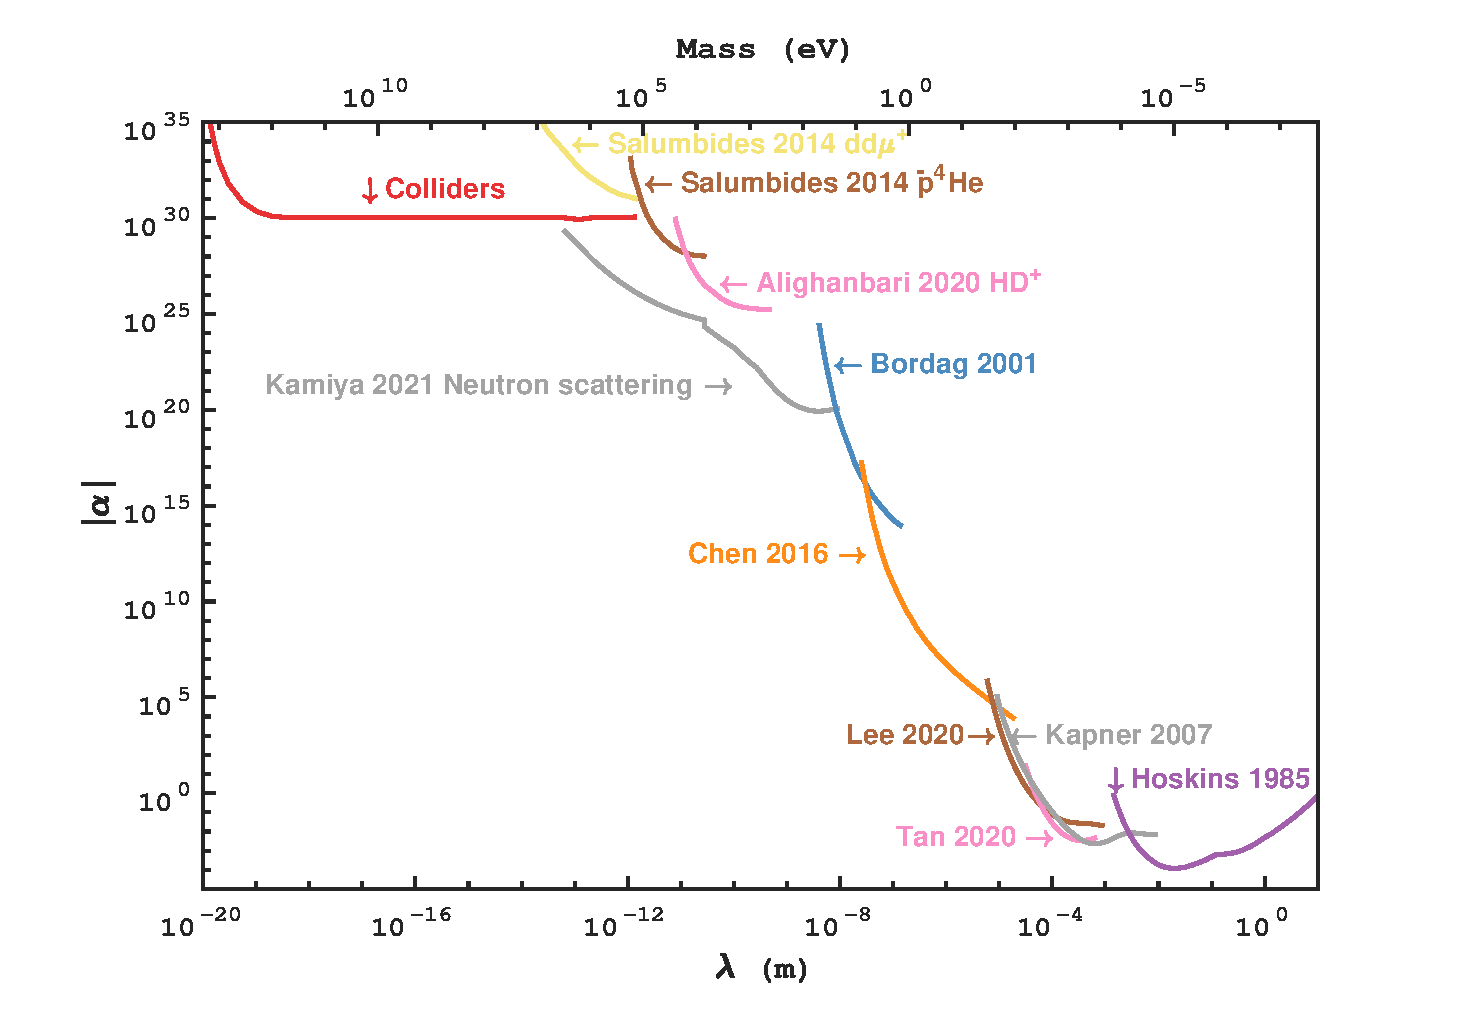
\includegraphics[width=0.98\textwidth]{Fig16.eps}
\end{center}
\caption{
Constraints on the universal dimensionless coupling parameter $\alpha$, defined in Eq.\,\eqref{gg-alpha_definition}, as a function of the interaction range $\lambda$ (or alternatively, new boson mass) for the potential term $V_{1}$. 
%\YS{I think ``Berg'' in ``Berg 2018'' is missing an accented ``e'' at the end. 
%{\color{red}Update (copied from main text): I just realised, upon closer inspection of the paper \citet{berge_microscope_2018}, that the MICROSCOPE bounds cannot be plotted in Figure\,\ref{alpha-fig}, since they're not sensitive to a universal test of the ISL in Eq.\,\ref{gg-alpha_definition}. The MICROSCOPE experiment measures differential accelerations of two pairs of test bodies made of different materials, which is sensitive to EP-violating forces, but not universal gravitational-type forces. In particular, Eqs.~(\ref{gsN-alpha}) and (\ref{gse-alpha}) don't apply for EP tests.} 
%\LC{Thank you for the explianation.}
%Some of the labels and accompanying arrows pointing to the curves seem to be separated from their respective curves; e.g., Bordag 2001, Kapner 2007, Hoskins 1985, Berg 2018. Technically, the y-axis should be the modulus of $\alpha$; i.e., $|\alpha|$.} 
}
\label{alpha-fig}
\end{figure*}


%%%% The follwoing part deleted by Lei after checking everything on April 17, 2024.
%\subsection{Macroscopic-scale bounds}\label{appendix_V1_Macro}
%{\color{red}YS [Update 2024/01/18]: I just realised, upon closer inspection of the paper \citet{berge_microscope_2018}, that the MICROSCOPE bounds cannot be plotted in Figure\,\ref{alpha-fig}, since they're not sensitive to a universal test of the ISL in Eq.\,\ref{gg-alpha_definition}. The MICROSCOPE experiment measures differential accelerations of two pairs of test bodies made of different materials, which is sensitive to EP-violating forces, but not universal gravitational-type forces. In particular, Eqs.~(\ref{gsN-alpha}) and (\ref{gse-alpha}) don't apply for EP tests. We can still place bounds from EP tests on $g_s g_s$ in Figure\,\ref{V1-fig}; e.g., by translating bounds from Fig.\,3 of \citet{grote_novel_2019}. Similar comments also apply to the ``Wagner 2012'' curve and probably also the ``EW 99'' curve (if it's the same as that in \cite{smith_short-range_1999}) in Figure\,\ref{alpha-fig}, since those experiments were EP tests and not ISL tests. The relevant bounds from those experiments can be obtained, e.g., by translating the bounds in Figure 1 and Table II of \citet{leefer_search_2016}.} 

%\LCa{Thank you for double check the result. I have removed these lines.} 
%\YS{Thank you, Lei!} 

%\sout{The most stringent macroscopic-scale bounds \YS{for long interaction ranges $\lambda$} were provided by \citet{berge_microscope_2018} (see Fig.\,2 in their paper \YS{If we're using relation (\ref{gsN-alpha}), then we should probably be using Berge's figure 1 for $q=B$, which scales with the number of nucleons. On the other hand, their figure 2 for $q= B-L$ scales with the number of neutrons.}), who analyzed torsion-pendulum experiments conducted in space, notably the MICROSCOPE mission \cite{touboul_microscope_2017}. It is worth mentioning that the final results of the MICROSCOPE mission have been released \cite{touboul_microscope_2022} \YS{and offer improved sensitivity to $g_s g_s$ by a factor of 4.6 compared to that in \cite{touboul_microscope_2017}}.} 

%\sout{Additional macroscopic-scale bounds can be found in \cite{wagner_torsion-balance_2012,talmadge_model-independent_1988}, derived from Lunar Laser Ranging (LLR) results \cite{turyshev_space-based_2007,williams_progress_2004,merkowitz_tests_2010}, focusing on the Earth-Moon differential acceleration toward the Sun, or the violation of inverse-square law obtained from anomalous precession of the lunar orbit. Furthermore, Keplerian tests which include planetary and satellite interactions provide further insights into these constraints.}

%\sout{For the scalar-nucleon coupling bound derived from MICROSCOPE's initial results, see Fig.\,3 of \citet{grote_novel_2019}. 
%\YS{Note that the final MICROSCOPE bounds on the scalar-nucleon coupling parameter $g_s^N$ are $\sqrt{4.6} \approx 2.1$ times stronger.} }

%\sout{For macroscopic-scale force searches with atomic spectroscopy and a summary of earlier macroscopic-scale torsion-pendulum experiments, see \citet{leefer_search_2016}, particularly Figure 1 and Table II, and references therein. }



%%%%
\subsection{Torsion-pendulum experiments}\label{appendix_V1_Torsion}
%\sout{In the interaction range around $10^{-3}$\,m, the most stringent constraint comes from the Eöt-Wash 2012 \cite{wagner_torsion-balance_2012} and Eöt-Wash 1999 \cite{smith_short-range_1999} experiments. }

An overview of the results is presented in Fig.\,\ref{alpha-fig}. 

In the interaction range $3 \times 10^{-3}\,\textrm{m} < \lambda < 10$\,m, there are results from Irvine, where 
\citet{spero_test_1980}; \citet{hoskins_experimental_1985} 
%\citet{spero_test_1980,hoskins_experimental_1985}
conducted torsion balance experiments. 

For interaction ranges around $\lambda \sim 10^{-4}$\,m, the Huazhong University of Science and Technology (HUST) group \cite{tan_improvement_2020} improved on their earlier research using a torsion balance \cite{tan_new_2016}. 

For the force range $10^{-5} \, \textrm{m} < \lambda <10^{-4}$\,m, the Washington group \cite{lee_new_2020} improved on their earlier Cavendish-type experiment results \cite{kapner_tests_2007} in a part of the range. 
\citet{kapner_tests_2007} outperformed the earlier work, such as Eöt-Wash 2004 \cite{hoyle_submillimeter_2004} and the results from Colorado \cite{long_upper_2003}, and partially on the Cavendish-type experimental result from Stanford \cite{chiaverini_new_2003,smullin_constraints_2005}. 


%%%
\subsection{Casimir force}
For the interaction range $10^{-7} \, \textrm{m} < \lambda <10^{-5}$\,m, the Indiana University–Purdue University (IUPU) collaboration \cite{chen_stronger_2016} %, \citeyear{chen_constraining_2022}
% \LC{check \citeyear{chen_constraining_2022}, it seems it is a aproposal and we should remove it here and update the bounds at some other places.} 
employed a technique that subtracts the otherwise dominant Casimir force, as demonstrated by IUPU \cite{decca_novel_2007,decca_tests_2007}, Yale \cite{sushkov_new_2011} and Stanford \cite{geraci_improved_2008} groups. 
%\YS{From memory, the Sushkov 2011 experiment was at Yale, but the Geraci 2008 experiment was at Stanford.}\LC{corrected.}


In the force range around $\lambda \sim 10^{-8}$\,m, the Riverside group (\citealp{mohideen_precision_1998};
\citealp{roy_demonstration_1999}; 
\citealp{klimchitskaya_complete_1999}; \citealp{harris_precision_2000}; \citealp{bordag_new_2001}, \citeyear{bordag_advances_2009})
%\cite{bordag_advances_2009,mohideen_precision_1998,klimchitskaya_complete_1999,roy_demonstration_1999,harris_precision_2000,bordag_new_2001} 
conducted a series of precision measurements of the Casimir force, providing the most stringent constraints on the interaction constants of Yukawa-type interactions using atomic force microscopy (AFM).
% , with data taken from \citet{bordag_new_2001}.


%%%%
\subsection{Neutron scattering, spectroscopy of exotic atoms, collider experiments}\label{appendix_V1_exotic}

%\LC{YS:check this paper \citet{voronin_search_2023}.}\LCa{done, not better than \cite{pokotilovski_constraints_2006}.}

%\LC{check if we include this paper, e.g. result for e-p from hydrogen \cite{munro-laylim_effects_2023} }

For the range $6 \times 10^{-14} \, \textrm{m} < \lambda < 8 \times 10^{-9}$\,m, neutron scattering (\citealp{pokotilovski_constraints_2006}; \citealp{kamiya_constraints_2015}; \citealp{haddock_search_2018-1}; \citealp{kamiya_experimental_2021})
%\cite{kamiya_experimental_2021,haddock_search_2018-1,kamiya_constraints_2015,pokotilovski_constraints_2006} 
established the most stringent constraints, involving scattering off xenon gas and $^{208}$Pb nuclei. 
Other neutron-scattering experiments include those of \citet{nesvizhevsky_neutron_2008,voronin_search_2023}. 
%\LC{Note that \cite{kamiya_experimental_2021} may have an error in Fig.\,2\,(d) where the unit GeV should be eV}. 
%\YS{I suspect that the presence of units on the y-axis of Figure 2(d) of the Kamiya 2021 paper is an error altogether. $g$ should probably be dimensionless, just like in figure 2(e) below. Another cross-check is that the Kamiya 2021 curve should intersect with the Bordag/Mohideen 2021 curve at roughly $\lambda \sim 10^{-8}\,\textrm{m}$ and $g^2 \sim 10^{-17}$, which should then be translated into a limit on $\alpha$. }
%\LCa{yes, the intersect point is correct in our figure. }
Within a similar range, research has been conducted based on antiprotonic helium atoms (for $\bar{p}$-$N$), $dd\mu^+$ \cite{salumbides_bounds_2014} (for $\mu^+$-$N$) and HD$^+$ \cite{alighanbari_precise_2020} (for $p$-$N$). For HD$^+$, see further work by \citet{germann_three-body_2021} and \citet{alighanbari_test_2023}. 
Furthermore, \citet{lemos_submillimeter_2021} provided prospective bounds (i.e., projections) for non-Newtonian gravity from spectroscopy by analyzing transitions between Rydberg states. 
%\YS{What is an ionic transition? Is this standard terminology in Rydberg atom physics?}\LC{it may not, i have removed the word "ionic".}

Over the range $10^{-20} \, \textrm{m} < \lambda < 6 \times 10^{-14}$\,m, 
%\YS{The upper $\lambda$ value may change depending on how the Kamiya curve shifts above. Regarding the lower $\lambda$ value, why do we cut off the graph in Fig.\,\ref{alpha-fig} at $10^{-19}$\,m instead of $10^{-20}$\,m?}, 
%\LC{updated}
the most stringent constraints are derived from collider experiments \cite{murata_review_2015}. 

For additional earlier constraints on short-range modifications of gravity or additional interactions, one can also refer to the reviews by \citet{adelberger_tests_2003,mostepanenko_state_2020}, among others. 


%%%%
%\subsection{Conversion of bounds on $\alpha$ to $g_sg_s$}
\subsection{\texorpdfstring{Conversion of bounds on $\alpha$ to $g_sg_s$}{Conversion of bounds on α to gsgs}}
\label{appendix_V1_alpha-to-gsgs}

The bounds on $|\alpha|$ are given with respect to the usual gravitational interaction strength, so in experiments that measure forces on test bodies, we can use the following relations [obtained by comparing Eq.\,(\ref{gg-alpha_definition}) and $V_1$ shown in Eq.\,(\ref{scalar-scalar_potential})] to obtain bounds on $\alpha$: 
\begin{equation}
\label{gsN-alpha}
    (g_s^N)^2 \approx 4 \pi |\alpha| \left(\frac{m_N}{M_\textrm{Pl}}\right)^2 \, , 
\end{equation}
where $M_\textrm{Pl}=\sqrt{\hbar c /G} \approx 1.2 \times 10^{19}\,\textrm{GeV}$ is the Planck mass, and 
\begin{equation}
\label{gse-alpha}
    (g_s^e)^2 \approx 4 \pi |\alpha| \left(\frac{m_N}{M_\textrm{Pl}}\right)^2  \frac{A_1 A_2}{Z_1  Z_2} \, , 
    %{\color{red}(g_s^e)^2 \approx 4 \pi |\alpha| (m_e / M_\textrm{Pl})^2 \left< Z_1 \right> \left< Z_2 \right> / (\left< A_1 \right> \left< A_2 \right>)} \, . 
\end{equation}
%\YS{
where $A_{1,2}$ and $Z_{1,2}$ are the nucleon and electron numbers, respectively, per atom in bodies 1 and 2.
%} 
%\YS{I think I made a mistake in the derivation of Eq.~(\ref{gse-alpha}). Since electrons contribute subdominantly to the overall mass of a test body, the sensitivity to $(g_s^e)^2$ should be degraded (rather than enhanced) by a factor of $(Z m_e) / (A m_N)$ at each test body. This gives the relation $(g_s^e)^2 = (g_s^N)^2 \times (\left< A_1 \right> \left< A_2 \right> m_N^2) / (\left< Z_1 \right> \left< Z_2 \right> m_e^2)$. Could we please check this? There are potentially important ramifications for the electron constraints shown in Fig.~\ref{V1-fig} that come from the $\alpha$ bounds in Fig.~\ref{alpha-fig} (like ``Torsion e-e'' and ``Casimir e-e''), as well as follow-on implications for curves in the main results figures that rely on the $V_1$ term for electrons (including direct bounds on $V_1$, and combined lab-astro bounds).} 
For typical moderately heavy elements, the average ratio of number of electrons to nucleons is $Z / A \approx 0.4$. 
Here $m_N$ denotes the average nucleon mass. 
%masses of the two fermion species rather than those of the two bodies used in the experiment. 

Note that we generally cannot use the above procedure to place bounds on cross-combinations of parameters like $g_s^Ng_s^e$. 
The reason is that to extract a bound on $g_s^N$ from one of the vertices, we make an assumption like $|g_s^N| \gg |g_s^e|$, while to extract a bound on $g_s^e$ from the other vertex, we make an assumption $|g_s^e| \gg |g_s^N|$, and so it is generally not possible to simultaneously satisfy both of these conditions. 
%\DB{Why do we need to make such assumptions? What does it mean ``to extract a bound on $g_s^N$ from a vertex'' ? Can both points be briefly clarified? } \YS{What 
If, for example, $g_s^N$ dominates the force contribution at one vertex (body), then $g_s^N$ will also generally dominate at the other vertex (body), and hence the (self-consistent) bound in this case would be on the product $g_s^N g_s^N$. 

For the constraints on $|\alpha|$ shown in Fig.\,\ref{alpha-fig}, at boson masses greater than $\sim 10^6$ eV, 
%\YS{This mass may change depending on how the Kamiya curve shifts above.}\LC{Should be fine.}
the most stringent constraints come from collider-based experiments. 
These collider-based bounds may not necessarily be simply translated to bounds on $(g_s^e)^2$ and $(g_s^N)^2$ in the way this is done for bounds from macroscopic tests of gravity. 
In high-energy collisions using protons at the Large Hadron Collider (LHC), it may not be appropriate to use nucleons as the degrees of freedom to describe the underlying interactions. 
Instead, one should describe interactions of exotic bosons in terms of their underlying interactions with quarks and gluons. 
In the case of electron interactions, one should consider other collider-based experiments that use accelerated electrons [e.g., the Large Electron-Positron (LEP) collider] -- these types of experiments operated at lower energies than the LHC (which reached peak energies of around 10\,TeV, whereas LEP operated at energies of about 100\,GeV), so the limits on electron couplings would be expected to start degrading at smaller boson masses. 
Therefore, since boson masses greater than $10^6$\,eV exceed the mass ranges in our $g_sg_s$ 
%{\color{red}and $g_Vg_V$} 
figures, we have not presented collider-based bounds in those figures. 
%\YS{Technically, the statement about boson masses greater than $10^6$\,eV in the previous sentence is only true for the $g_s g_s$ figures, but not the $g_V g_V$ figures. Maybe we can remove reference to the $g_V g_V$ case here (as an extra justification for this, this subsection focuses purely on the $g_s g_s$ case).} 

%\LC{We may incorporate this paragraph into the above one?} 
%\YS{I think we now discuss the key points in the paragraph above.} 
%YV:I looked into these references and a few of the references in the Murata and Tanaka paper from 2015.  From what I've understood, it seems that these collider-based bounds come from analyses at experiments at the LHC and LEP (as well as Tevatron), which were interpreted in terms of models of massive gravitons and extra dimensions. Basically, these massive gravitons are produced in the collisions of electrons (at LEP) or protons (at LHC) and can then subsequently decay into jets of practically any type of standard-model particles (since all standard-model particles are affected by gravity).  Those analyses effectively place limits on combinations of interactions of a boson with various different standard-model particles, hence we can't simply rescale those bounds on alpha into bounds on ${g_s^e}^2$ or ${g_s^N}^2$ without performing an analysis on a specific channel (like, e.g., electron-positron pair production in the case of LEP) or knowing how much that specific channel contributes to the total cross section.  Unless we decide to look into these sorts of details. 



%%%%
%\subsection{Converting other constraints from precision spectroscopy to bounds on $g_sg_s$}
\subsection{\texorpdfstring{Converting other constraints from precision spectroscopy to bounds on $g_sg_s$}{Converting other constraints from precision spectroscopy to bounds on gsgs}}
\label{appendix_V1_PS}

%\LCa{question to YS: constraints from precision spectroscopy to $g_sg_s$ ca also be converted to $g_Vg_V$?}

There are constraints from precision spectroscopy presented as bounds on spin-independent couplings of exotic bosons to electrons, protons, and neutrons. 
These couplings are occasionally denoted as $y_e$, $y_p$, and $y_n$, respectively, where within the theoretical framework utilized in this review, $y_X$ is equivalent to $g_s^X$. 


%%%
\subsubsection*{a. $g_s^e g_s^e$ and $g_s^e g_s^{e^+}$} 
Bounds on $g_s^e g_s^{e^+}$ from positronium spectroscopy were presented by \citet{adkins_precision_2022} and are not much weaker than bounds on $g_s^e g_s^e$ from the electron magnetic moment ($g$-factor) reported by \citet{delaunay_probing_2017}. 
There are other bounds on electron-electron interactions, see \citet{frugiuele_current_2019}; \citet{debierre_fifth-force_2020}.
%\citet{frugiuele_current_2019, debierre_fifth-force_2020}. 


%%%
\subsubsection*{b. $g_s^eg_s^n$} 
\citet{delaunay_probing_2017} provided one of the most stringent constraints on $g_s^eg_s^n$ and there are other constraints from \citet{berengut_probing_2018}; \citet{debierre_fifth-force_2020}; \citet{solaro_improved_2020}; \citet{sailer_measurement_2022}; \citet{door_search_2024}.
%\citet{door_search_2024,solaro_improved_2020,berengut_probing_2018,debierre_fifth-force_2020,sailer_measurement_2022}.


%%%
\subsubsection*{c. $g_s^eg_s^{{\mu}^+}$} 
The Mu-MASS Collaboration \cite{ohayon_precision_2022} and \citet{frugiuele_current_2019} both studied $1S-2S$ measurements in muonium. 
In our figures, for clarity, we have only included the results from \citet{ohayon_precision_2022}. 
These measurements strictly apply to the matter-antimatter combination $g_s^eg_s^{\mu^+}$. 

In addition, there are astrophysical bounds on $(g_s^{\mu})^2$ provided by \citet{caputo_muonic_2022}, which can be found in Tab.\,\ref{tabel_Astrophysical-bounds}. 
There are also ongoing and proposed experiments, such as muonium free-fall experiments in the context of the combination of parameters $g_s^eg_s^{{\mu}^+}$, as detailed by \citet{stadnik_searching_2023} and references therein. 
The parameters $\Lambda_e$ and $\Lambda_{\mu}$ in Fig.\,2 of \citet{stadnik_searching_2023} are related to the parameters $g_s^e$ and $g_s^{\mu}$ via the relationships $g_s^e = m_e/\Lambda_e$ and $g_s^{\mu} = m_{\mu}/\Lambda_{\mu}$, respectively. 

We have provided a comprehensive overview of bounds on Yukawa-type interactions in Fig.\,\ref{V1-fig} for reference. 
The strongest bounds from this collection are featured in the main-text figures. 

\begin{figure*} [!htbp]
\begin{center}
%\includegraphics[width=0.98\textwidth]{gsgscompare.eps}
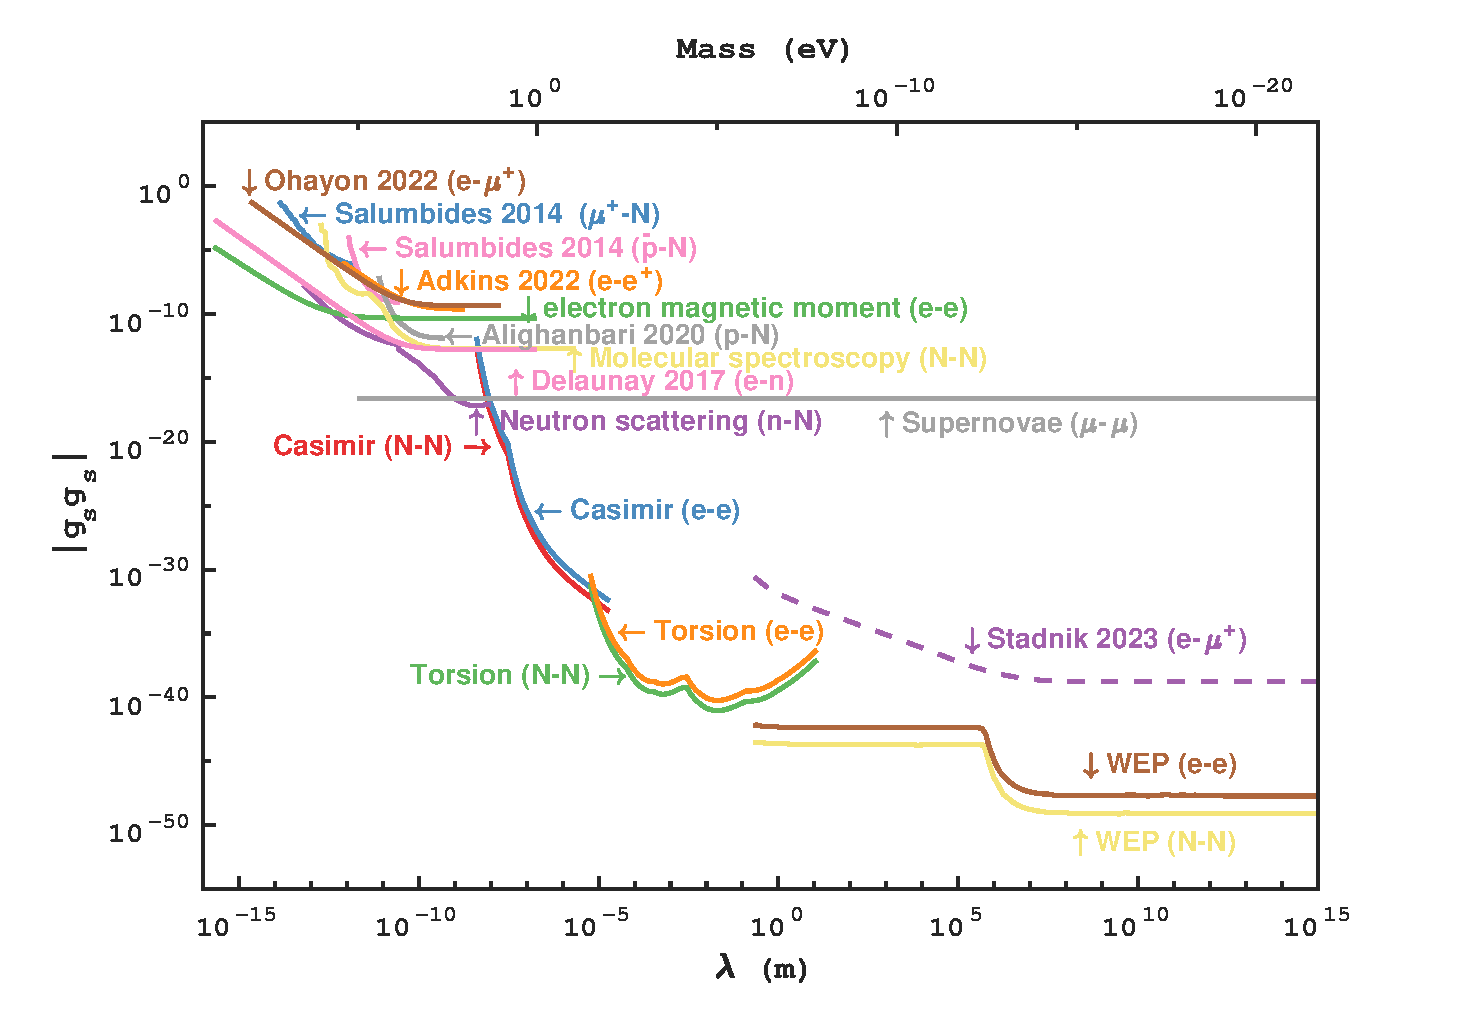
\includegraphics[width=0.98\textwidth]{Fig17.eps}
\end{center}
\caption{
%\YS{{\color{red} The ``Torsion e-e'' and ``Casimir e-e'' curves may need to be updated. Please see the discussion around Eq.~(\ref{gse-alpha}).} } 
Constraints on $g_sg_s$ as a function of the interaction range $\lambda$ (or alternatively, the mass of the new scalar boson). 
%\LC{Done.}
%\YS{Thank you for updating, Lei!}
%\LC{\cite{ohayon_precision_2022} should be e-\textmu.} 
%\YS{\color{green} I think the current Ohayon 2022 label (with antimuon) is technically correct, assuming that they refer to muonium (which contains an electron and anti-muon).}\LC{OK.}
%\YS{Some of the labels and accompanying arrows pointing to the curves seem to be separated from their respective curves. Regarding the torsion experimental limits, are these only from tests of the ISL? \LC{Now in the updated figure, yes.} 
%\YS{Thnak you, Lei!}
%\YS{What about also including torsion-pendulum-based limits from EP tests (where the nucleon bounds should be more comparable to the electron bounds)?\LC{Added}} 
%\YS{Thank you for adding, Lei. Is it possible to double check the EEP (e-e) curve? Using the curve for $\Lambda_e$ from \cite{grote_novel_2019}, I find an estimate for the EEP (e-e) curve that is approximately of the same strength as the current EEP (N-N) curve. (There may be follow-on implications for some of the results graphs in the main text.)} \LCa{Oh, I see. I have updated it. I take $\Lambda_{\gamma}$ previously.} 
%\YS{Thank you for checking and updating, Lei! I think this may affect some of the combined and $V_1$-based limits in the results graphs in Sec.~\ref{Sec:limits_main}, such as $g_V g_V$, $g_s g_s$, $g_s g_p$, etc. Is it possible to double-check the relevant curves?}\LC{done}
}
\label{V1-fig}
\end{figure*}


%%%
%\subsection{Constraints on $g_sg_s$ from tests of the weak equivalence principle (WEP)}
\subsection{\texorpdfstring{Constraints on $g_sg_s$ from tests of the weak equivalence principle (WEP)}{Constraints on gsgs from tests of the weak equivalence principle (WEP)}}
\label{Appendix:WEP_tests}

%\YS{Technically, there are two types of equivalence principle (EP): the strong EP and the weak EP. For clarity, could we please replace ``Einstein equivalence principle (EEP)'' by ``weak equivalence principle (WEP)'' in the title of this subsection and the usage of EEP by WEP throughout this (and other) subsection(s)?}
%\LC{yes}

The satellite-based MICROSCOPE experiment \cite{touboul_microscope_2017} measured differential accelerations between two pairs of test bodies made of different materials, which are sensitive to WEP-violating forces but insensitive to  universal gravitational-type forces. 
In particular, Eqs.\,\eqref{gsN-alpha} and \eqref{gse-alpha} are not applicable to WEP tests. 
% \DB{Could you kindly explicitly state why this is so?} \YS{Certainly. Eqs.\,\eqref{gsN-alpha} and \eqref{gse-alpha} apply to searches for universal fifth forces which (like gravity) preserve the WEP. In searches for WEP violation, such universal forces affect the pairs of test masses identically and hence their effect cancels in a differential acceleration measurement.} 
Nonetheless, we can still place bounds from WEP tests on $g_s g_s$ in Fig.\,\ref{V1-fig} by translating the bounds, for example, from \citet{leefer_search_2016}; \citet{grote_novel_2019}.
%\citet{grote_novel_2019, leefer_search_2016}. 
It is noteworthy that the final MICROSCOPE bound of \citet{touboul_microscope_2022} can be re-scaled from their 2017 result in \citet{touboul_microscope_2017} by a factor of 4.6 improvement, though we do not present this improved bound here. Similar analysis have been performed for gauge vector boson couplings to baryons and leptons in \cite{fayet_microscope_2018,fayet_microscope_2019}.

%\subsection{Equivalence of constraints on $g_sg_s$ and $g_Vg_V$ from ${V}_1$}
\subsection{\texorpdfstring{Equivalence of constraints on $g_sg_s$ and $g_Vg_V$ from ${V}_1$}{Equivalence of constraints on gsgs and gVgV from V1}}
\label{appendix_V1_gsgs-and-gvgv}
The ${V}_1$ potential term in the scalar/scalar [see Eq.\,(\ref{gsgs_V1})] and vector/vector [see Eq.\,(\ref{gVgV_V1})] cases only differ by an overall sign, so there's no difference when presenting bounds on the modulus of coupling parameters $|g_s g_s|$ and $|g_V g_V|$. 
Thus, we can translate limits in the $\alpha-\lambda$ parameter space to limits in the $g^X_Vg^Y_V-\lambda$ parameter space in the same way.

%\begin{equation}
%\label{gg-alpha_translation_relation}
%g^X_Vg^Y_V=-4\pi \frac{m_Xm_Y}{M_I}\alpha
%\end{equation}
%Note same as Eq.\,\eqref{gsN-alpha} and \ref{gse-alpha} , $m_X$ and $m_Y$ here denote the masses of the two fermion species rather than those of the two bodies used in the experiment. 
%Here we take $G=6.6743 \times 10^{-11} \rm{m}^3\rm{kg}^{-1}\rm{s}^{-2})$. 
%\YS{One could in principle alternatively/also quote $G = 1/M_{\rm{Pl}}^2$ with $M_{\rm{Pl}} \approx 1.2 \times 10^{19}\,\rm{GeV}$ here and assume $\hbar = c =1$ in Eq.~(\ref{gg-alpha_translation_relation}). Either way, the notations/conventions/choice of units should be consistent; e.g., we currently have explicit factors of $\hbar$ and $c$ appearing in Eq.~(\ref{gVgV_V1}), but use $\hbar = c = 1$ in Eq.~(\ref{vector-vector_potential}).} \LC{yes, will check and sure  consistent. }



%%%%%%%%%%%%%%%%%%%%%%%%%%%%%%%%%%%%%%%%%%%%%%%%%%%%%%
                      % App3 
%%%%%%%%%%%%%%%%%%%%%%%%%%%%%%%%%%%%%%%%%%%%%%%%%%%%%%

%\section{Astrophysical bounds}\label{appendixC}


%%%%
\section{Bounds for the purpose of comparison}
\label{appendix_comp.}

In Appendix \ref{appendix_V1}, we present the constraints arising from the spin-independent potential term $V_1$, which can serve as a basis for comparison with constraints on $g_sg_s$ and $g_Vg_V$ from other spin-dependent potential terms. 
Additionally, in Sec.\,\ref{METH2.Astro.}, we discuss astrophysical limits, which are also valuable for comparison. 
In this section, we discuss combined astrophysical-laboratory bounds, which are also used for comparison, in addition to presenting individual constraints from the $V_1$ term and from astrophysics. 


%%%%
\subsection*{1. $g_Vg_A$}
For $g_V g_A$ (see Fig.\,\ref{gvga-fig}), we present combined astrophysical-laboratory bounds. 
There are two ways of constructing such bounds. 

One way is to take astrophysical bounds on $g_A^e$ and $g_A^N$ (see Tab.\,\ref{tabel_Astrophysical-bounds}). We also take laboratory bounds on $g_V$ from the $V_1$ potential term; 
specifically, we take constraints on $g_V^e$ from the electron magnetic moment, Casimir experiments, torsion-pendulum experiments and WEP experiments, and $g_V^N$ from the molecular spectroscopy, Casimir experiments, torsion-pendulum experiments and WEP experiments.
%{\color{green}$g_V^N$ from the latter three types of experiments}. 
%\YS{In principle, we can compensate the loss of the electron magnetic moment bound for $g_V^N$ by the addition of the molecular spectroscopy (N-N) bounds to probe boson masses greater than about $10^2$\,eV. Should we mention this here and extend the relevant combined results figures in the main text accordingly [Figs.\,\ref{gvga-fig}\,(b) and (c)]?}\LC{Yes, done.} 
Then we multiply these bounds to obtain constraints on $g_A g_V$. 

Another way is to take the best laboratory bounds for $g_A$ (from the spin-dependent 
%{\color{red}$V_3$ term} \YS{
$V_2$ and $V_3$ terms) 
%?}
and astrophysical bounds from $g_V$ (see Tab.\,\ref{tabel_Astrophysical-bounds}). 
The resulting bounds on $g_A g_V$ diverge as $\propto 1/M$ in the limit as $M \to 0$. 
(In contrast, the scaling is $\propto 1/M^2$ for the $g_A g_A$ case, and is independent of $M$ for all of the other vertex combinations considered in our review). 
We do not present this result for clarity %{\color{red}in the figure} \YS{
in Fig.\,\ref{gvga-fig}.
%?}. 

%I think the pseudovector/vector case is a bit special and somewhat different also from the pseudovector/pseudovector case.


%%%%
\subsection*{2. $g_Ag_A$}\label{appendix_comp.gAgA}

For $g_Ag_A$ (see Figs.\,\ref{gaga-fig1} and \ref{gaga-fig2}), we can present both purely astrophysical bounds and combined astrophysical-laboratory bounds. 

Regarding astrophysical bounds, Eq.\,(31) from \citet{dror_dark_2017} gives bounds on the electron and nucleon axial-vector couplings (see Tab.\,\ref{tabel_Astrophysical-bounds}). 
We plot $g_A^e g_A^e$, $g_A^e g_A^N$, and $g_A^N g_A^N$ for comparison. 
We use, for example, $g_A^eg_A^N \leq [(g_A^e)^2+(g_A^N)^2]/2$ obtained from the identity $(g_A^e-g_A^N)^2\geq0$. 

Regarding combined astrophysical-laboratory bounds, for $g_A g_A$, we can use the best available $g_A^e$ lab bounds (from the %{\color{red}$V_3$ term} \YS{
$V_2$ and $V_3$ terms)
%?}) 
and combine them with a bound on $g_A^e$ or $g_A^N$ from astrophysics. 
We do not present this result in the figure to avoid clutter. 

We also present analogous electron $g$-factor bounds for the purely axial-vector case in Fig.\,\ref{gaga-fig1} using Eq.\,(6) from \citet{karshenboim_constraints_2014}, which for our purposes reads: $g_A^eg_A^e=[g_V^e M/(\sqrt{2} m_e)]^2$ in the limit $M \ll m_e$. 
$g_V^e$ here are electron $g$-factor bounds based on a $V_1$-type term [taken from \citet{delaunay_probing_2017}]. 
Note that the resulting bound on $g_A^2$ diverges like $\propto 1/M^2$ in the limit of small $M$, which is due to the non-conservation of the axial-vector current. 


%%%%
\subsection*{3. $g_Vg_V$}

For $g_Vg_V$ (see Fig.\,\ref{gVgV-fig}), we present astrophysical bounds, as well as laboratory bounds on the spin-independent $V_1$ term. 
We do not present the (weaker) combined astrophysical-laboratory bounds to avoid cluttering the figure. %(which are typically much stronger than the best laboratory bounds over most of the considered boson masses). 

In the case of astrophysical bounds, we plot constraints on $g_V^e g_V^e$, $g_V^e g_V^N$ and $g_V^N g_V^N$. 
Constraints on $g_V^e g_V^N$ can be calculated just like for $g_A^e g_A^N$ as discussed above. 
%in Sec.\,\ref{appendix_comp.gAgA}. 

For laboratory bounds based on the spin-independent $V_1$ term, see App.\,\ref{appendix_V1}. 


%%%%
\subsection*{4. $g_pg_s$}
For $g_pg_s$ (see Fig.\,\ref{gpgs-fig}), we present astrophysical and combined astrophysical-laboratory bounds.

For the combined astrophysical-laboratory bounds, we take astrophysical bounds on the $g_p$ couplings from the literature (see Tab.\,\ref{tabel_Astrophysical-bounds}) and multiply them by laboratory bounds on $g_s$ couplings from $V_1$-type searches. 

For the purely astrophysical bounds, we can proceed as follows. 
Assuming that both $g_s$ and $g_p$ couplings are present, astrophysical energy-loss-type bounds constrain combinations of parameters like $a g_s^2 + b g_p^2$. 
The ratio of the dimensionless coefficients $a,b$ is not necessarily equal to 1. 
For the sake of simplicity, let us suppose that $a=b=1$; in this case, we know that $(g_s - g_p)^2 \ge 0 \Rightarrow g_s g_p \le (g_s^2 + g_p^2) / 2$, which allows us to constrain the combination $g_s g_p$. 

%\LCa{Is the following comments from \citet{poddar_constraints_2023} useful?}
%\YS{Yes! I've reworded the paragraph a little bit.}\LC{Thanks!}
%\LC{consider also adding this comment: The previous lab-astro bounds on gSgP obtained in the literature are derived from two different observations. In these studies, the monopole coupling gS and the dipole coupling gP are measured independently from two different observations and they are simply multiplied to get bound on gSgP. To get bound in this way is overly stringent and may not be completely reliable if the axion changes its behavior in different environments. The bounds on gSgP obtained from lab-lab experiments are only valid for the axions of mass \textmu eV. ma. meV. (Poddar and Pachhar, 2023, p. 12)}
Regarding the combination of different types of bounds, if one combines bounds from two independent measurements taken in vastly different environments (e.g., if the bounds on $g_s$ come from lab-based measurements, whereas the bounds on $g_p$ are derived from measurements in hot or dense astrophysical environments), then the resulting bounds on the product of coupling constants (in this example, on $g_s g_p$) may not be robust if the properties of the boson involved change in different environments. 
See, for example, \citet{poddar_constraints_2023} for discussion of this point. 



%\LC{[For astrophysical-bounds, see Table\,\ref{tabel_Astrophysical-bounds}]. The below are original comments from Yevgeny and we keep them here for the record:}\YS{ \citet{raffelt_particle_1999} gives the following stellar bounds on the scalar couplings: $g_s^e \lesssim 1.3 \times 10^{-14}$ and $g_s^N \lesssim 4.3 \times 10^{-11}$ for scalar masses $\lesssim \mathcal{O}(\textrm{keV})$. 
%Study of the evolution of red-giant stars constrains the pseudoscalar electron coupling to be $g_p^e \lesssim 1.5 \times 10^{-13}$ for sub-keV masses; see \citet{straniero_rgb_2020} and \citet{capozzi_axion_2020}. 
%Study of white-dwarf cooling constraints the pseudoscalar electron coupling to be $g_p^e \lesssim 1.4 \times 10^{-13}$ for sub-keV masses; see \citet{bertolami_revisiting_2014}. 
%Study of neutron-star cooling constraints the pseudoscalar-neutron coupling to be $g_p^n \lesssim 3 \times 10^{-10}$ for masses $\lesssim 10~\textrm{keV}$; see \citet{beznogov_constraints_2018}, while the application of energy-loss arguments to supernova SN1987A constrains the pseudoscalar nucleon coupling to be $g_p^N \lesssim 10^{-9}$; see \citet{carenza_improved_2019}. 
%Application of energy-loss arguments to SN1987A constrains the pseudoscalar-muon coupling to be $g_p^\mu \lesssim 10^{-8}$ for masses $\lesssim 30~\textrm{MeV}$; see \citet{bollig_muons_2020,bollig_erratum_2021}, while \citet{caputo_muonic_2022} gives the globular cluster bound on the scalar-muon coupling to be $g_s^\mu \lesssim 5 \times 10^{-9}$ for masses $\lesssim 100~\textrm{keV}$. }



%%%%
\subsection*{5. $g_pg_p$}
%The purely astrophysical bounds are already good.

%\LC{For $g_pg_p$ ($e$-$e$, $e$-$N$, $N$-$N$), we also take one $g_p$ from astrophysics and another one $g_p$ from $V_3$? That will be in total 4 lines.} \YS{We could in principle do this. Unlike the $g_sg_s$ case above, some $V_3$-type laboratory experiments use either predominantly spin-polarized electrons or spin-polarized nucleons. If the $V_3$ laboratory experiment uses, e.g., spin-polarized electrons, then one can in principle take $g_p^e\ll g_p^N$ in order to combine the laboratory bound on $g_p^e$ with the astrophysical bound on $g_p^N$. I'm not sure, however, that we need to present such combined laboratory-astrophysical bounds on $g_pg_p$ since the purely astrophysical bounds are already much stronger.}


For $g_pg_p$ (see Fig.\,\ref{gpgp-fig}), we present astrophysical bounds (see Tab.\,\ref{tabel_Astrophysical-bounds}) and $g$-factor-based bounds. 

%We add astrophysical bounds here for comparison. 
%As shown in Tab.\, \ref{tabel_Astrophysical-bounds}, we have: Study of the evolution of red-giant stars constrains the pseudoscalar electron coupling to be $g_p^e \lesssim 1.5 \times 10^{-13}$ for sub-keV masses; see \citet{straniero_rgb_2020} and \citet{capozzi_axion_2020}. 
%Study of white-dwarf cooling constraints the pseudoscalar electron coupling to be $g_p^e \lesssim 1.4 \times 10^{-13}$ for sub-keV masses; see \citet{bertolami_revisiting_2014}. 
%Study of neutron-star cooling constraints the pseudoscalar-neutron coupling to be $g_p^n \lesssim 3 \times 10^{-10}$ for masses $\lesssim 10~\textrm{keV}$; see \citet{beznogov_constraints_2018}, while the application of energy-loss arguments to supernova SN1987A constrains the pseudoscalar nucleon coupling to be $g_p^N \lesssim 10^{-9}$; see \citet{carenza_improved_2019}. 
%Application of energy-loss arguments to SN1987A constrains the pseudoscalar-muon coupling to be $g_p^\mu \lesssim 10^{-8}$ for masses $\lesssim 30~\textrm{MeV}$; see \citet{bollig_muons_2020,bollig_erratum_2021}. 

For the $e$-$e$ and $e$-$\mu$ $g$-factor-based bounds, we take the limits presented in 
%{\color{red}Figs.\,5 and 6} \YS{
Figs.\,3 and 6
%} 
of \citet{frugiuele_current_2019}, respectively. 
%\YS{
[Note that the captions to Figs.\,3 and 5 in \citet{frugiuele_current_2019} are mixed up.]
%} 

%For the $e$-$e$ g-factor-based bound, we take the limits from \citet{delaunay_probing_2017}. 
%For the $e$-$\mu$ g-factor bound, we take the constraints from \cite{ohayon_precision_2022}. 
%\YS{Strictly speaking, what's presented in the Ohayon 2022 paper isn't a bound from $g$-factors, but rather the region of parameters required to resolve the muon $g$-factor anomaly, if one combines bounds from the electron $g$-factor as well.}\LC{Em, shall we accept the comment and make some modification of the content here? Shall we still keep the line in the figure? }
%\YS{Sorry, I just read this again and realised that neither \cite{delaunay_probing_2017} nor \cite{ohayon_precision_2022} actually constrained $g_p g_p$, but rather they constrained $g_s g_s$. 
%I think the ``Ohayon 2022 ($e-\mu$)'' curve in Figure~\ref{V1-fig} is correct, but it comes from the comparison of measurements and theory of the $1s - 2s$ interval in muonium (rather than from $g$-factors). I think this discussion needs to be moved to the subsection ``$g_s g_s$'' below. In its place here, we should find the relevant references for $g$-factor-based bounds on $g_p g_p$.} \LC{Ok, then I will remove the two line from the figure for in $g_pg_p$. The e-e interaction from \citet{delaunay_probing_2017} is already in the figures for $g_sg_s$. We can mention Ohayon 2022 ($e-\mu$) from the comparison of measurements and theory of the $1s - 2s$ interval in muonium could be added to the $g_sg_s$ figure (a) in text. } 
%\LCa{See if we can find the relevant references for $g$-factor-based bounds on $g_p g_p$.}
%\YS{There is a constraint on $g_p^e g_p^\mu$ based on the $g$-factors of the electron and muon presented in Figure 6 of \cite{frugiuele_current_2019}, based on references [14-16] therein. Maybe those references contain the relevant information we need here?} \LC{Ok, results from figure 5 and figure 6 have been taken and presented in our $g_pg_p$ figure.}

%\YS{I think the above text and the \cite{delaunay_probing_2017} reference for the purely electron-based $g$-factor-based bound and the \cite{ohayon_precision_2022} reference for the mixed electron-muon $g$-factor-based bound can be moved to the subsection on $g_s g_s$ below.} \LC{\cite{delaunay_probing_2017} has been used, I will add the the \cite{ohayon_precision_2022} reference for the mixed electron-muon $g$-factor-based bound.} 


%There are also limits on the pseudoscalar-pseudoscalar coupling for the electron-(anti)electron and electron-(anti)muon combinations from the consideration of measurements (and comparison with theoretical predictions) of $g$-factors of the electron and muon and the frequencies of various transitions in positronium and muonium presented in Figures 5 and 6 of \citet{frugiuele_current_2019} -- please note that the figures (but not captions) for Figures 3 and 5 appear to be mixed up -- also note that electron $g$-factor limits on $g_p^e g_p^e$ should in principle be the same as those in \citet{yan_constraining_2019}. %According to \citet{andreas_constraints_2010}, the muon $g$-factor constraint is (in translated form) given by $g_p^\mu \lesssim 8 \times 10^{-4}$ for masses $\lesssim m_\mu$. 

%For other constraints, one can refer to Sec.\,VI in \cite{ohare_cornering_2020}. 



%%%%
\subsection*{6. $g_sg_s$}
For $g_s g_s$ (see Fig.\,\ref{gsgs-fig}), we present the best constraints from Fig.\,\ref{V1-fig} and separate purely astrophysical constraints. 
We also include constraints in Fig.\,\ref{gsgs-fig}\,(a) for $e$-$\mu^+$ which is the $g$-factor result from \citet{ohayon_precision_2022}. 
%\YS{Could we please double-check that the relevant curve in our Fig.\,\ref{gsgs-fig}\,(a) matches the orange band/curve in Fig.\,4 of \citet{ohayon_precision_2022}? It looks like our curve already starts to weaken at boson masses around $10^3$ eV, whereas the \citet{ohayon_precision_2022} curve only seems to start weakening at somewhat higher boson masses.} \LC{We take the black line from Fig.\,4 of \citet{ohayon_precision_2022}. If we want to present the g-factor result, then we should make a change to use the orange band. Should we use the lower boundary of the orange band?} {\color{red}YS: Thank you for explaining, Lei. The black line in Fig.~4 of \citet{ohayon_precision_2022} was actually based on the $1S$-$2S$ interval in muonium. I would probably use the upper boundary of the solid (rather than hatched) orange band - the reason is that the shaded region isn't excluded, but going above the shaded region would become excluded, since the interaction becomes too strong in that case.} 
%\LC{Ok, updated. The result in Fig 16 is still the 1s-2s result.}
%By the way, should we label the Ohayon 2022 ($e$-$\mu$) line in Fig. 16 to be Ohayon 2022 ($e$-$\mu^+$)?}


%Besides of the constraints for $e$-$e$, $e$-$N$ and $N$-$N$ interaction, there are also $g_sg_s$ constraints for $e$-$\mu^+$ \cite{ohayon_precision_2022,stadnik_searching_2023}, $e$-$e^+$ \cite{adkins_precision_2022}, $\mu$-$\mu$ \cite{caputo_muonic_2022}, as discussed in Sec.\,\ref{appendix_V1_PS}.

%I would propose to present only the purely astrophysical bounds in this case. \YS{I propose to add astrophysical limits here too. 
%From before: 
%\citet{raffelt_particle_1999} gives the following stellar bounds on the scalar couplings: $g_s^e \lesssim 1.3 \times 10^{-14}$ and $g_s^N \lesssim 4.3 \times 10^{-11}$ for scalar masses $\lesssim \mathcal{O}(\textrm{keV})$. 
%\cite{caputo_muonic_2022} gives the globular cluster bound on the scalar-muon coupling $g_s^\mu \lesssim 5 \times 10^{-9}$ for masses $\lesssim 100~\textrm{keV}$. }



%\LCa{We could in principle improve this $g_S^N$. \cite{chen_stronger_2016} has been improved by \cite{chen_constraining_2022}. And we could even present a wider range of $g_S^N$ as presented in Fig.\,\ref{alpha-fig}. However, (modify the following content)}

%YS: Not combined astrophysical-laboratory constraints.

In the literature [see, e.g., \citet{kim_experimental_2018}], there exist combined astrophysical-laboratory bounds. These incorporate the bounds on $g_s^e$ derived from stellar cooling rates \cite{grifols_constraints_1986,jain_evading_2006} and laboratory bounds on $g_s^N$ from recent searches for hypothetical (spin-independent) Yukawa interactions (\citealp{chen_stronger_2016}; \citealp{tan_improvement_2020}; \citealp{lee_new_2020}),
%\cite{chen_stronger_2016,tan_improvement_2020,lee_new_2020}, 
as discussed by \citet{raffelt_limits_2012} and \citet{leslie_prospects_2014}. 

%{\color{red}Need to update this paragraph.} 
%However, these combined astrophysical-laboratory bounds are model-dependent. 
%The laboratory bounds of interest typically constrain a combination of $g_s^N$ and $g_s^e$ with a relative weighting coefficient that is in favour of the $g_s^N$ coupling by a few orders of magnitude, and similarly the astrophysical bounds constrain a combination of $(g_s^N)^2$ and $(g_s^e)^2$ with a relative weighting coefficient that can potentially differ from unity by a roughly similar amount. \DB{Similar to what?} \YS{I've rewritten this paragraph in a new form below. Please check to see if this is clearer now.} 
%Therefore, if one assumes that $g_s^N$ dominates in the $V_1$ laboratory bound, then it should typically also dominate in the astrophysical bound. 
%In this sense, combined astrophysical-laboratory bounds on $g_s^N g_s^e$ may not necessarily be self-consistent. 

%\YS{New version of above paragraph: 
%The laboratory bounds of interest typically constrain a combination of $g_s^N$ and $g_s^e$ with a relative weighting coefficient that is in favour of the $g_s^N$ coupling by a few orders of magnitude, while astrophysical bounds on $g_s^e$ are generally stronger than those on $g_s^N$ by a few orders of magnitude. 
%Therefore, combined astrophysical-laboratory bounds on $g_s^N g_s^e$ may not necessarily be self-consistent. } 

%{\color{red}YS: New version of paragraph: 
The laboratory bounds of interest typically constrain the combination of parameters $(a_1 g_s^N + b_1 g_s^e)(a_2 g_s^N + b_2 g_s^e)$, where $a_{1,2}$ and $b_{1,2}$ are dimensionless coefficients that are specific to the source and test masses used in the experiment; e.g., for fifth-force searches using torsion-pendulum experiments and Casimir-force measurements, as well as WEP tests, the typical ratio of coefficients is $a_{1,2}/b_{1,2} \sim 1$. 
On the other hand, astrophysical bounds constrain the combination of parameters $c (g_s^N)^2 + d (g_s^e)^2$, where the typical ratio of coefficients is $d/c \sim 10^6 - 10^7$. 
Depending on the relative sizes of the coupling constants $g_s^e$ and $g_s^N$, the resulting (dominant) combined astrophysical-laboratory bounds may be on the combination $(g_s^N)_\textrm{lab} \times (g_s^e)_\textrm{astro}$, $(g_s^e)_\textrm{lab} \times (g_s^e)_\textrm{astro}$ or $(g_s^N)_\textrm{lab} \times (g_s^N)_\textrm{astro}$. 
%}


The situation is different when one combines, for example, astrophysical bounds on $g_p$ with $V_1$-type laboratory bounds on $g_s$. 
In that case, those particular laboratory experiments tend to be practically insensitive to $g_p$, so one may assume $g_p \gg g_s$ to isolate the $g_p$ part of the astrophysical bounds, which are strictly on the combination of parameters $a g_s^2+ b g_p^2$, with the ratio $a/b \sim 1$. 



%%%%%%%%%%%%%%%%%%%%%%%%%%%%%%%%%%%%%%%%%%%%%%%%%%%%%%
                      % App4 
%%%%%%%%%%%%%%%%%%%%%%%%%%%%%%%%%%%%%%%%%%%%%%%%%%%%%%


%%%%%%%%%%%%%%%%%%%%%%%%%%%%%%%%%%%%%%%%%%%%%%%%%%%%%%
                      % App5 
%%%%%%%%%%%%%%%%%%%%%%%%%%%%%%%%%%%%%%%%%%%%%%%%%%%%%%

\section{Units, symbols and abbreviations}\label{appendixF}

\subsection*{1. Units}
The International System of Units or \textit{Système International} (SI) is used in the main results section Sec.\,\ref{Sec:limits_main} for the convenience of experimentalists. 
In the International System of Units, the units used are meter (m) for length, kilogram (kg) for mass, and second (s) for time. 
The fundamental constants $\hbar$ and $c$ appear explicitly in these units. 

Natural units are predominantly employed in high-energy physics, particularly in particle physics and cosmology. 
The natural units are used in the theoretical framework section (Sec.\,\ref{Sec:formalism}), where $\hbar=c=1$. 

Atomic units are commonly used in atomic, molecular and optical physics. 
In these units, the elementary charge  $e$, electron mass $m_{\rm e}$, reduced Planck constant $\hbar$ and vacuum permittivity $\epsilon_0$ are set to $e=m_{\rm e}=\hbar = 4\pi\epsilon_0=1$, which implies that the speed of light in vacuum is $c= 137$. 

Each unit system helps to make particular calculations or theoretical developments more intuitive and/or less cluttered. 
%Independently of the confusion to change between these two sets of units, it is essential to develop a specific intuition about characteristic scales in natural units. This is very important to correctly identify the mass range of novel particles susceptible to affect spectroscopic observables in atomic and molecular systems. Therefore, we believe that it is worth introducing the basics of natural units and how they relate to atomic units. In natural units, mass M using the celebrated Einstein’s relation, $E = mc^2$, is equivalent to energy, which implies that the unit of mass is GeV/c2. For instance, the mass of the electron is $511 \times 10^{-6} GeV/c^2$. In natural units, length L and time T have the same units, and taking into account $\hbar c = 1$ leads to $\lambda ≡ T = 1/E$, and their units are $c^2/GeV$. To transform from natural units to atomic units is essential to keep in mind that $\lambda = \hbar c/E$, and in atomic units $c= 137$. 

%As a result, one finds $\frac{1}{GeV/c^2} = \frac{511 \times 10^{-6}} {137} a_0 = 3.73 \times 10^{−6} a_0$ where $a_0$ is the Bohr radius ($a_0 = 0.529177 × 10^{-10} m$). Therefore, the unit of length in natural units is tiny in comparison with the typical extension of atomic and molecular systems. Similarly, it is possible to invert such expression to find that $a_0 = 1/3.73 {(keV/c^2)}^{-1}$. In this section, when analyzing the existence of new particles we explore a mass range between 10 $MeV/c^2$ and 0.1 $keV/c^2$, which corresponds to a length of $3.73\times10^{-4} a_0$ and $37.3 a_0$, respectively. \cite{adkins_precision_2022}.


%%%%
\subsection*{2. Symbols and abbreviations}
For ease of reference, the most common mathematical abbreviations and symbols are systematically listed in Tables \ref{Table:symbols} and \ref{Table:abbreviations}. 
These tables do not include terms that are limited to specific subtopics or that are only occasionally used; however, these terms are defined when they are first used. It should be noted that the chosen notations and abbreviations are consistent with those that are commonly used in the existing literature. 


%\LC{I have removed these we do not need. Next, we add these missing.}\YS{This sounds good.}

\begin{table}
\caption{Mathematical symbols used and their meanings. 
%\YS{Technically, $g$ can be either the Land\'{e} $g$-factor of a particle or the regular $g$-factor of a particle. Maybe put Land\'{e} in parentheses below?} 
%\YS{I couldn't find where the symbol $\theta_\textrm{W}$ is used in the main text. Maybe we can remove this entry from the table if we don't use it in the main text?} 
%\YS{I propose making this table ``full'' two-column width so that the bottom-most entries can also fit on a single page. The section hyperlinks should be updated (or removed if we don't need them).}
}
\renewcommand{\arraystretch}{1.2} % Adjust the line spacing here
\medskip \begin{tabular}{ll} \hline \hline
Symbol~~~~~~ & Meaning \\
\hline
\rule{0ex}{2.6ex} $c$ & speed of light in vacuum\\
%\rule{0ex}{2.6ex} $\epsilon_0$ & electric constant \YS{``vacuum permittivity'' is more common} \\
\rule{0ex}{2.6ex} $G$ & Newtonian constant of gravitation\\
\rule{0ex}{2.6ex} $h$ & Planck constant\\
               &also reduced Planck constant $\hbar=h/(2\pi$) \\
%\rule{0ex}{2.6ex} {\textit{e}} & elementary \YS{electric} charge \\
%\rule{0ex}{2.6ex}  $\alpha$ & \YS{electromagnetic} fine-structure constant \\
%\rule{0ex}{2.6ex} $R_{\infty}$ & Rydberg constant \\
%\rule{0ex}{2.6ex}  $a_0$ & Bohr radius \\
%\rule{0ex}{2.6ex} $\mu_\mr{N}$ & nuclear magneton \\
%\rule{0ex}{2.6ex}  $G_\mr{F}$ & Fermi constant \\
\rule{0ex}{2.6ex} $g$  & local acceleration due to Earth's gravity \\ 
                       &or %{\color{red}Land\'{e}}
                       (Land\'{e}) $g$-factor of a particle\\
%\rule{0ex}{2.6ex} \LC{$g_J$}  & Land\'{e} $g$-factor\\
%\rule{0ex}{2.6ex} \LC{$\mu$}  & magnetic moment of the atom\\
%\rule{0ex}{2.6ex}   & \LC{This one need check}\\
\rule{0ex}{2.6ex}  $m_{e}$ & electron mass \\
\rule{0ex}{2.6ex}  $m_{p}$ & proton mass \\
\rule{0ex}{2.6ex}  $m_{N}$ & average nucleon mass \\
%\rule{0ex}{2.6ex}  $M_Z$ & $Z$-boson mass \\
%\rule{0ex}{2.6ex} {\color{red}$\theta_\mr{W}$} & {\color{red}weak mixing angle}\\
\rule{0ex}{2.6ex}  $\sigma_{i}$ & Pauli matrices, $i=1,2,3$ \\
\rule{0ex}{2.6ex} $\gamma_{e,N}$ & gyromagnetic ratios of the electron or nucleus \\
\rule{0ex}{2.6ex} $\gamma _\mu$ & Dirac matrices, $\mu=0,1,2,3$ \\
\rule{0ex}{2.6ex} $\gamma _5$ & $\gamma_5 = i \gamma^0 \gamma^1 \gamma^2 \gamma^3$ \\ % Dirac matrix associated with pseudoscalars\\
\rule{0ex}{2.6ex} $\sigma^{\mu \nu}$ & $\sigma^{\mu \nu}=\frac{i}{2}\left( \gamma^\mu \gamma^\nu - \gamma^\nu \gamma^\mu \right)$\\
%\rule{0ex}{2.6ex} $\v{s}$ & single electron spin \\
%\rule{0ex}{2.6ex} $\v{S}$ & \YS{total electron spin in an atom} \\
%multi-electron atom total spin\\
\rule{0ex}{2.6ex} $\v{p}$ & linear momentum \\
\rule{0ex}{2.6ex} $\v{E}$ & electric field (vector)\\
\rule{0ex}{2.6ex} $\v{B}$ & magnetic field (vector)\\
\rule{0ex}{2.6ex} $C, P, T$ & charge conjugation, spatial inversion, and \\
\rule{0ex}{2.6ex} & time reversal discrete transformations\\
%\rule{0ex}{2.6ex}  $\mu=m_{p}/m_{e}$ & proton to electron mass ratio, $\overline{\mu}=1/\mu$ (Sec.\,\ref{Sec:FC})\\
%\rule{0ex}{2.6ex}  $K_\alpha$& dimensionless sensitivity factor of an energy level\\
%                      & to $\alpha$-variation (Sec.\,\ref{Sec:FC})\\
%\rule{0ex}{2.6ex}  $K_\mu$& dimensionless sensitivity factor of an energy level\\
 %                         & to $\mu$-variation (Sec.\,\ref{Sec:FC}) \YS{In \textit{variations} of fundamental constants, we use the convention $\mu=m_e/m_p$, which is opposite to the convention in the \textit{determination} of fundamental constants quoted a few lines above}\\
 %   \rule{0ex}{2.6ex}  $m_{q}$ & average of light quark masses (Sec.\,\ref{Sec:FC})\\
\rule{0ex}{2.6ex}  $\Lambda_{\mr{QCD}}$& quantum chromodynamics (QCD) energy scale\\
%\rule{0ex}{2.6ex}  $\kappa$& dimensionless sensitivity factor of an energy level\\
 %           & to a variation of $X_q=m_q/\Lambda_{\mr{QCD}}$ (Sec.\,\ref{Sec:FC})\\
 %\rule{0ex}{2.6ex}           $k_X$& dimensionless factor quantifying the spatial\\
 % \rule{0ex}{2.6ex}    &  variation of the fundamental constant $X$ (Sec.\,\ref{Sec:FC})\\
\rule{0ex}{2.6ex} $Q_\mr{W}$ & nuclear weak charge \\
%\rule{0ex}{2.6ex}  $\v{d}$ & electric dipole moment \YS{(EDM)} (Sec.\,\ref{Sec:EDM})\\
%\rule{0ex}{2.6ex}  $\mathcal{P}$ & dimensionless electrical polarization (Sec.\,\ref{Sec:EDM}) \\
%\rule{0ex}{2.6ex}  \hbox{\boldmath{$\mathcal{S}$}} & Schiff moment\\
%\rule{0ex}{2.6ex}  $\tilde{d}$ & chromo-EDM (Sec.\,\ref{Sec:EDM}) \\
\rule{0ex}{2.6ex} $\v{\sigma}$ & unit vector along spin\\
\hline \hline
\end{tabular}
\label{Table:symbols}
\end{table}



\begin{table}
\caption{Abbreviations and their meanings. 
%\YS{Maybe we can remove the entry for EEP here if we decide to replace its usage by WEP in the rest of the paper?} 
}
\renewcommand{\arraystretch}{1.2} % Adjust the line spacing here
\medskip \begin{tabular}{ll} \hline \hline
Abbreviation~~ & Meaning \\
\hline
%\rule{0ex}{2.6ex} AMO & atomic, molecular and optical physics \\
\rule{0ex}{2.6ex} ALPs & axionlike particles \\
\rule{0ex}{2.6ex} APV & atomic parity violation \\
\rule{0ex}{2.6ex} atm & atmosphere, a unit of measurement used\\
                      & to express pressure\\
\rule{0ex}{2.6ex} CPT & combined $CPT$ discrete transformation \\
\rule{0ex}{2.6ex} CPV & $CP$-violation \\
%\rule{0ex}{2.6ex} cEDM & chromo-electric dipole moment \\
\rule{0ex}{2.6ex} c.m. & center of mass\\% \YS{Why not use the capitalised ``C.M.'' instead?} \\
\rule{0ex}{2.6ex} DFSZ & Dine-Fischler-Srednicki-Zhitnitsky (axion) \\
\rule{0ex}{2.6ex} DM & dark matter \\
\rule{0ex}{2.6ex} EDM & electric dipole moment \\
%\rule{0ex}{2.6ex} {\color{red}EEP} & \color{red}Einstein equivalence principle} \\
\rule{0ex}{2.6ex} ESR & electron spin resonance \\
%\rule{0ex}{2.6ex} eEDM & electron EDM \\
\rule{0ex}{2.6ex} GDM & gravitational dipole moment \\
%\rule{0ex}{2.6ex} GR & general relativity ?\\
%\rule{0ex}{2.6ex} GPS & Global Positioning System \\
%\rule{0ex}{2.6ex} GW & gravitational wave \\
%\rule{0ex}{2.6ex} HCI & highly charged ion \\
\rule{0ex}{2.6ex} ISL & inverse-square law \\
\rule{0ex}{2.6ex} KSVZ & Kim-Shifman-Vainshtein-Zakharov (axion) \\
\rule{0ex}{2.6ex} LHC & Large Hadron Collider \\
%\rule{0ex}{2.6ex} LLI& local Lorentz invariance\\
%\rule{0ex}{2.6ex} LPI& local position invariance\\
%\rule{0ex}{2.6ex} LV & Lorentz symmetry violation \\
%\rule{0ex}{2.6ex} MWDM & Moody-Wilczek-Dobrescu-Mocioiu \YS{Do we use this abbreviation in this review?} \\
%\rule{0ex}{2.6ex} MQM & magnetic quadrupole moment \\
%\rule{0ex}{2.6ex} NAM & nuclear anapole moment \\
%\rule{0ex}{2.6ex} NIST & National Institute of Standards and Technology \\
\rule{0ex}{2.6ex} NMR & nuclear magnetic resonance \\
%\rule{0ex}{2.6ex} NR &  nonrelativistic \\ %\YS{Why not use the capitalised ``NR'' instead?} \\
\rule{0ex}{2.6ex} PNC & parity nonconservation\\
\rule{0ex}{2.6ex} PV & parity violation\\
%\rule{0ex}{2.6ex} PSP & permutation-symmetry postulate\\
\rule{0ex}{2.6ex} QCD & quantum chromodynamics \\
\rule{0ex}{2.6ex} QED & quantum electrodynamics \\
\rule{0ex}{2.6ex} SERF & spin-exchange relaxation-free \\
\rule{0ex}{2.6ex} SM & standard model \\
%\rule{0ex}{2.6ex} SME & Standard Model extension\\
%\rule{0ex}{2.6ex} SMt & Schiff moment \\
%\rule{0ex}{2.6ex} STM & scanning tunneling microscope \\
\rule{0ex}{2.6ex} SQUID & Superconducting Quantum\\
                        &Interference Device \\
%\rule{0ex}{2.6ex} SCCEF & Sun-Centered Celestial Equatorial Frame \\
%\rule{0ex}{2.6ex} SST & spin-statistics theorem \\
%\rule{0ex}{2.6ex} SUSY & supersymmetry \\
%\rule{0ex}{2.6ex} T,PV  & simultaneous $T$- and $P$-violation \\
%\rule{0ex}{2.6ex} TV & $T$-violating but $P$-conserving  \\
%\rule{0ex}{2.6ex} VULF & virialized ultralight field \\
\rule{0ex}{2.6ex} UBDM & ultralight bosonic dark matter\\
\rule{0ex}{2.6ex} UCN & ultra-cold neutrons\\
\rule{0ex}{2.6ex} WEP & weak equivalence principle\\
\rule{0ex}{2.6ex} WIMP & weakly-interacting massive particle \\
%\rule{0ex}{2.6ex} UFF & universality of free fall\\
\hline \hline
\end{tabular}
\label{Table:abbreviations}
\end{table}


\newpage
%\LC{below may be used in the introduction part, already modified according to YS's comments. }
%\YS{Thank you, Lei! I've updated the text below a bit. Yes, we could potentially use this content in the introduction, possibly with some rearrangement/modification.} 
%\LCa{Thank you for the revision, Zhenia. Let's decide where to put it later.}
%\YS{This sounds good!}

%In quantum mechanics, particles can have either integer spin (0, 1, 2, etc.) or half-integer spin (1/2, 3/2, 5/2, etc.). Integer spin particles are called bosons, while half-integer spin particles are called fermions.

%A pseudoscalar or pseudovector (axial-vector) particle are types of bosons that have integral spin, but they also have an additional property called parity. Parity is a measure of the symmetry of a system under the simultaneous inversion of all spatial coordinates (or equivalently, a reflection and a rotation). Under inversion of spatial coordinates, an even-parity state or wavefunction remains unchanged, whereas an odd-parity state or wavefunction changes sign.

%Pseudoscalars are particles that have odd parity. There are no known elementary pseudoscalars in nature, but some examples of composite pseudoscalars observed in nature include pions and kaons. Pseudoscalars are also of interest in cosmology, as they can be produced in the early universe and may contribute to the dark matter content of the universe.

%Pseudovectors are particles that have even parity. An example of pseudovectors includes the magnetic field. Being vector-type (spin-1) fields, pseudovectors have both a direction and a magnitude.Pseudovectors (axial-vectors) transform in the same way as vectors under rotations. The difference between axial vectors and polar vectors arises in terms of how they transform under the inversion of spatial coordinates. Examples of pseudovector particles include pseudovector mesons, which are composite particles made up of quark-antiquark pairs. 
%} 


%%%
%\bibliographystyle{apsrev4-1}
%\bibliographystyle{apsrmp4-2}
\addcontentsline{toc}{section}{References}
%\bibliographystyle{apsrmp4-2}
%\bibliography{MyLibrary}
%apsrmp4-2.bst 2018-12-27 (MD) hand-edited version of apsrmp4-1.bst
%Control: key (0)
%Control: author (75) reversed first initials jnrlst
%Control: editor formatted (0) differently from author
%Control: production of article title (-1) disabled
%Control: page (0) single
%Control: year (1) truncated
%Control: production of eprint (0) enabled
\providecommand{\noopsort}[1]{}
\begin{thebibliography}{721}%
\makeatletter
\providecommand \@ifxundefined [1]{%
 \@ifx{#1\undefined}
}%
\providecommand \@ifnum [1]{%
 \ifnum #1\expandafter \@firstoftwo
 \else \expandafter \@secondoftwo
 \fi
}%
\providecommand \@ifx [1]{%
 \ifx #1\expandafter \@firstoftwo
 \else \expandafter \@secondoftwo
 \fi
}%
\providecommand \natexlab [1]{#1}%
\providecommand \enquote  [1]{``#1''}%
\providecommand \bibnamefont  [1]{#1}%
\providecommand \bibfnamefont [1]{#1}%
\providecommand \citenamefont [1]{#1}%
\providecommand \href@noop [0]{\@secondoftwo}%
\providecommand \href [0]{\begingroup \@sanitize@url \@href}%
\providecommand \@href[1]{\@@startlink{#1}\@@href}%
\providecommand \@@href[1]{\endgroup#1\@@endlink}%
\providecommand \@sanitize@url [0]{\catcode `\\12\catcode `\$12\catcode
  `\&12\catcode `\#12\catcode `\^12\catcode `\_12\catcode `\%12\relax}%
\providecommand \@@startlink[1]{}%
\providecommand \@@endlink[0]{}%
\providecommand \url  [0]{\begingroup\@sanitize@url \@url }%
\providecommand \@url [1]{\endgroup\@href {#1}{\urlprefix }}%
\providecommand \urlprefix  [0]{URL }%
\providecommand \Eprint [0]{\href }%
\providecommand \doibase [0]{https://doi.org/}%
\providecommand \selectlanguage [0]{\@gobble}%
\providecommand \bibinfo  [0]{\@secondoftwo}%
\providecommand \bibfield  [0]{\@secondoftwo}%
\providecommand \translation [1]{[#1]}%
\providecommand \BibitemOpen [0]{}%
\providecommand \bibitemStop [0]{}%
\providecommand \bibitemNoStop [0]{.\EOS\space}%
\providecommand \EOS [0]{\spacefactor3000\relax}%
\providecommand \BibitemShut  [1]{\csname bibitem#1\endcsname}%
\let\auto@bib@innerbib\@empty
%</preamble>
\bibitem [{\citenamefont {Aad}\ \emph {et~al.}(2012)\citenamefont {Aad},
  \citenamefont {Abajyan}, \citenamefont {Abbott}, \citenamefont {Abdallah},
  \citenamefont {Khalek}, \citenamefont {Abdelalim}, \citenamefont {Aben},
  \citenamefont {Abi}, \citenamefont {Abolins}, \citenamefont {AbouZeid} \emph
  {et~al.}}]{aad_observation_2012}%
  \BibitemOpen
  \bibfield  {author} {\bibinfo {author} {\bibnamefont {Aad}, \bibfnamefont
  {G.}}, \bibinfo {author} {\bibfnamefont {T.}~\bibnamefont {Abajyan}},
  \bibinfo {author} {\bibfnamefont {B.}~\bibnamefont {Abbott}}, \bibinfo
  {author} {\bibfnamefont {J.}~\bibnamefont {Abdallah}}, \bibinfo {author}
  {\bibfnamefont {S.~A.}\ \bibnamefont {Khalek}}, \bibinfo {author}
  {\bibfnamefont {A.~A.}\ \bibnamefont {Abdelalim}}, \bibinfo {author}
  {\bibfnamefont {R.}~\bibnamefont {Aben}}, \bibinfo {author} {\bibfnamefont
  {B.}~\bibnamefont {Abi}}, \bibinfo {author} {\bibfnamefont {M.}~\bibnamefont
  {Abolins}}, \bibinfo {author} {\bibfnamefont {{\relax OS}.}~\bibnamefont
  {AbouZeid}},  \emph {et~al.}} (\bibinfo {year} {2012}),\ \href@noop {}
  {\bibfield  {journal} {\bibinfo  {journal} {Phys. Lett. B}\ }\textbf
  {\bibinfo {volume} {716}}~(\bibinfo {number} {1}),\ \bibinfo {pages}
  {1}}\BibitemShut {NoStop}%
\bibitem [{\citenamefont {Abbott}\ and\ \citenamefont
  {Sikivie}(1983)}]{abbott_cosmological_1983}%
  \BibitemOpen
  \bibfield  {author} {\bibinfo {author} {\bibnamefont {Abbott}, \bibfnamefont
  {L.~F.}}, and\ \bibinfo {author} {\bibfnamefont {P.}~\bibnamefont {Sikivie}}}
  (\bibinfo {year} {1983}),\ \href
  {https://doi.org/10.1016/0370-2693(83)90638-X} {\bibfield  {journal}
  {\bibinfo  {journal} {Phys. Lett. B}\ }\textbf {\bibinfo {volume}
  {120}}~(\bibinfo {number} {1}),\ \bibinfo {pages} {133}}\BibitemShut
  {NoStop}%
\bibitem [{\citenamefont {Abe}\ \emph {et~al.}(2024)\citenamefont {Abe},
  \citenamefont {Hogan}, \citenamefont {Kaplan}, \citenamefont {Overstreet},\
  and\ \citenamefont {Rajendran}}]{abe_search_2024}%
  \BibitemOpen
  \bibfield  {author} {\bibinfo {author} {\bibnamefont {Abe}, \bibfnamefont
  {M.}}, \bibinfo {author} {\bibfnamefont {J.~M.}\ \bibnamefont {Hogan}},
  \bibinfo {author} {\bibfnamefont {D.~E.}\ \bibnamefont {Kaplan}}, \bibinfo
  {author} {\bibfnamefont {C.}~\bibnamefont {Overstreet}}, and\ \bibinfo
  {author} {\bibfnamefont {S.}~\bibnamefont {Rajendran}}} (\bibinfo {year}
  {2024}),\ \href {https://doi.org/10.48550/arXiv.2409.14793} {}\Eprint
  {https://arxiv.org/abs/2409.14793} {arXiv:2409.14793} \BibitemShut {NoStop}%
\bibitem [{\citenamefont {Abel}\ \emph {et~al.}(2020)\citenamefont {Abel},
  \citenamefont {Afach}, \citenamefont {Ayres}, \citenamefont {Baker},
  \citenamefont {Ban}, \citenamefont {Bison}, \citenamefont {Bodek},
  \citenamefont {Bondar}, \citenamefont {Burghoff}, \citenamefont {Chanel}
  \emph {et~al.}}]{abel_measurement_2020}%
  \BibitemOpen
  \bibfield  {author} {\bibinfo {author} {\bibnamefont {Abel}, \bibfnamefont
  {C.}}, \bibinfo {author} {\bibfnamefont {S.}~\bibnamefont {Afach}}, \bibinfo
  {author} {\bibfnamefont {N.~J.}\ \bibnamefont {Ayres}}, \bibinfo {author}
  {\bibfnamefont {C.~A.}\ \bibnamefont {Baker}}, \bibinfo {author}
  {\bibfnamefont {G.}~\bibnamefont {Ban}}, \bibinfo {author} {\bibfnamefont
  {G.}~\bibnamefont {Bison}}, \bibinfo {author} {\bibfnamefont
  {K.}~\bibnamefont {Bodek}}, \bibinfo {author} {\bibfnamefont
  {V.}~\bibnamefont {Bondar}}, \bibinfo {author} {\bibfnamefont
  {M.}~\bibnamefont {Burghoff}}, \bibinfo {author} {\bibfnamefont
  {E.}~\bibnamefont {Chanel}},  \emph {et~al.}} (\bibinfo {year} {2020}),\
  \href {https://doi.org/10.1103/PhysRevLett.124.081803} {\bibfield  {journal}
  {\bibinfo  {journal} {Phys. Rev. Lett.}\ }\textbf {\bibinfo {volume}
  {124}}~(\bibinfo {number} {8}),\ \bibinfo {pages} {081803}}\BibitemShut
  {NoStop}%
\bibitem [{\citenamefont {Abel}\ \emph {et~al.}(2023)\citenamefont {Abel},
  \citenamefont {Ayres}, \citenamefont {Ban}, \citenamefont {Bison},
  \citenamefont {Bodek}, \citenamefont {Bondar}, \citenamefont {Chanel},
  \citenamefont {Crawford}, \citenamefont {Daum}, \citenamefont {Dechenaux}
  \emph {et~al.}}]{abel_search_2023}%
  \BibitemOpen
  \bibfield  {author} {\bibinfo {author} {\bibnamefont {Abel}, \bibfnamefont
  {C.}}, \bibinfo {author} {\bibfnamefont {N.~J.}\ \bibnamefont {Ayres}},
  \bibinfo {author} {\bibfnamefont {G.}~\bibnamefont {Ban}}, \bibinfo {author}
  {\bibfnamefont {G.}~\bibnamefont {Bison}}, \bibinfo {author} {\bibfnamefont
  {K.}~\bibnamefont {Bodek}}, \bibinfo {author} {\bibfnamefont
  {V.}~\bibnamefont {Bondar}}, \bibinfo {author} {\bibfnamefont
  {E.}~\bibnamefont {Chanel}}, \bibinfo {author} {\bibfnamefont {C.~B.}\
  \bibnamefont {Crawford}}, \bibinfo {author} {\bibfnamefont {M.}~\bibnamefont
  {Daum}}, \bibinfo {author} {\bibfnamefont {B.}~\bibnamefont {Dechenaux}},
  \emph {et~al.}} (\bibinfo {year} {2023}),\ \href
  {https://doi.org/10.21468/SciPostPhys.15.2.058} {\bibfield  {journal}
  {\bibinfo  {journal} {SciPost Physics}\ }\textbf {\bibinfo {volume}
  {15}}~(\bibinfo {number} {2}),\ \bibinfo {pages} {058}}\BibitemShut {NoStop}%
\bibitem [{\citenamefont {Abel}\ \emph {et~al.}(2017)\citenamefont {Abel},
  \citenamefont {Ayres}, \citenamefont {Ban}, \citenamefont {Bison},
  \citenamefont {Bodek}, \citenamefont {Bondar}, \citenamefont {Daum},
  \citenamefont {Fairbairn}, \citenamefont {Flambaum}, \citenamefont
  {Geltenbort}, \citenamefont {Green}, \citenamefont {Griffith}, \citenamefont
  {{\noopsort{grinten}}{van der Grinten}}, \citenamefont {Gruji{\'c}},
  \citenamefont {Harris}, \citenamefont {Hild}, \citenamefont {Iaydjiev},
  \citenamefont {Ivanov}, \citenamefont {Kasprzak}, \citenamefont {Kermaidic},
  \citenamefont {Kirch}, \citenamefont {Koch}, \citenamefont {Komposch},
  \citenamefont {Koss}, \citenamefont {Kozela}, \citenamefont {Krempel},
  \citenamefont {Lauss}, \citenamefont {Lefort}, \citenamefont {Lemi{\`e}re},
  \citenamefont {Marsh}, \citenamefont {Mohanmurthy}, \citenamefont
  {Mtchedlishvili}, \citenamefont {Musgrave}, \citenamefont {Piegsa},
  \citenamefont {Pignol}, \citenamefont {Rawlik}, \citenamefont {Rebreyend},
  \citenamefont {Ries}, \citenamefont {Roccia}, \citenamefont {Rozp{\k e}dzik},
  \citenamefont {{Schmidt-Wellenburg}}, \citenamefont {Severijns},
  \citenamefont {Shiers}, \citenamefont {Stadnik}, \citenamefont {Weis},
  \citenamefont {Wursten}, \citenamefont {Zejma},\ and\ \citenamefont
  {Zsigmond}}]{abel_search_2017}%
  \BibitemOpen
  \bibfield  {author} {\bibinfo {author} {\bibnamefont {Abel}, \bibfnamefont
  {C.}}, \bibinfo {author} {\bibfnamefont {N.~J.}\ \bibnamefont {Ayres}},
  \bibinfo {author} {\bibfnamefont {G.}~\bibnamefont {Ban}}, \bibinfo {author}
  {\bibfnamefont {G.}~\bibnamefont {Bison}}, \bibinfo {author} {\bibfnamefont
  {K.}~\bibnamefont {Bodek}}, \bibinfo {author} {\bibfnamefont
  {V.}~\bibnamefont {Bondar}}, \bibinfo {author} {\bibfnamefont
  {M.}~\bibnamefont {Daum}}, \bibinfo {author} {\bibfnamefont {M.}~\bibnamefont
  {Fairbairn}}, \bibinfo {author} {\bibfnamefont {V.~V.}\ \bibnamefont
  {Flambaum}}, \bibinfo {author} {\bibfnamefont {P.}~\bibnamefont
  {Geltenbort}}, \bibinfo {author} {\bibfnamefont {K.}~\bibnamefont {Green}},
  \bibinfo {author} {\bibfnamefont {W.~C.}\ \bibnamefont {Griffith}}, \bibinfo
  {author} {\bibfnamefont {M.}~\bibnamefont {{\noopsort{grinten}}{van der
  Grinten}}}, \bibinfo {author} {\bibfnamefont {Z.~D.}\ \bibnamefont
  {Gruji{\'c}}}, \bibinfo {author} {\bibfnamefont {P.~G.}\ \bibnamefont
  {Harris}}, \bibinfo {author} {\bibfnamefont {N.}~\bibnamefont {Hild}},
  \bibinfo {author} {\bibfnamefont {P.}~\bibnamefont {Iaydjiev}}, \bibinfo
  {author} {\bibfnamefont {S.~N.}\ \bibnamefont {Ivanov}}, \bibinfo {author}
  {\bibfnamefont {M.}~\bibnamefont {Kasprzak}}, \bibinfo {author}
  {\bibfnamefont {Y.}~\bibnamefont {Kermaidic}}, \bibinfo {author}
  {\bibfnamefont {K.}~\bibnamefont {Kirch}}, \bibinfo {author} {\bibfnamefont
  {H.-C.}\ \bibnamefont {Koch}}, \bibinfo {author} {\bibfnamefont
  {S.}~\bibnamefont {Komposch}}, \bibinfo {author} {\bibfnamefont {P.~A.}\
  \bibnamefont {Koss}}, \bibinfo {author} {\bibfnamefont {A.}~\bibnamefont
  {Kozela}}, \bibinfo {author} {\bibfnamefont {J.}~\bibnamefont {Krempel}},
  \bibinfo {author} {\bibfnamefont {B.}~\bibnamefont {Lauss}}, \bibinfo
  {author} {\bibfnamefont {T.}~\bibnamefont {Lefort}}, \bibinfo {author}
  {\bibfnamefont {Y.}~\bibnamefont {Lemi{\`e}re}}, \bibinfo {author}
  {\bibfnamefont {D.~J.~E.}\ \bibnamefont {Marsh}}, \bibinfo {author}
  {\bibfnamefont {P.}~\bibnamefont {Mohanmurthy}}, \bibinfo {author}
  {\bibfnamefont {A.}~\bibnamefont {Mtchedlishvili}}, \bibinfo {author}
  {\bibfnamefont {M.}~\bibnamefont {Musgrave}}, \bibinfo {author}
  {\bibfnamefont {F.~M.}\ \bibnamefont {Piegsa}}, \bibinfo {author}
  {\bibfnamefont {G.}~\bibnamefont {Pignol}}, \bibinfo {author} {\bibfnamefont
  {M.}~\bibnamefont {Rawlik}}, \bibinfo {author} {\bibfnamefont
  {D.}~\bibnamefont {Rebreyend}}, \bibinfo {author} {\bibfnamefont
  {D.}~\bibnamefont {Ries}}, \bibinfo {author} {\bibfnamefont {S.}~\bibnamefont
  {Roccia}}, \bibinfo {author} {\bibfnamefont {D.}~\bibnamefont {Rozp{\k
  e}dzik}}, \bibinfo {author} {\bibfnamefont {P.}~\bibnamefont
  {{Schmidt-Wellenburg}}}, \bibinfo {author} {\bibfnamefont {N.}~\bibnamefont
  {Severijns}}, \bibinfo {author} {\bibfnamefont {D.}~\bibnamefont {Shiers}},
  \bibinfo {author} {\bibfnamefont {Y.~V.}\ \bibnamefont {Stadnik}}, \bibinfo
  {author} {\bibfnamefont {A.}~\bibnamefont {Weis}}, \bibinfo {author}
  {\bibfnamefont {E.}~\bibnamefont {Wursten}}, \bibinfo {author} {\bibfnamefont
  {J.}~\bibnamefont {Zejma}}, and\ \bibinfo {author} {\bibfnamefont
  {G.}~\bibnamefont {Zsigmond}}} (\bibinfo {year} {2017}),\ \href
  {https://doi.org/10.1103/PhysRevX.7.041034} {\bibfield  {journal} {\bibinfo
  {journal} {Phys. Rev. X}\ }\textbf {\bibinfo {volume} {7}}~(\bibinfo {number}
  {4}),\ \bibinfo {pages} {041034}}\BibitemShut {NoStop}%
\bibitem [{\citenamefont {{ACME
  Collaboration}}(2014)}]{acme_collaboration_order_2014}%
  \BibitemOpen
  \bibfield  {author} {\bibinfo {author} {\bibnamefont {{ACME
  Collaboration}},}} (\bibinfo {year} {2014}),\ \href
  {https://doi.org/10.1126/science.1248213} {\bibfield  {journal} {\bibinfo
  {journal} {Science}\ }\textbf {\bibinfo {volume} {343}}~(\bibinfo {number}
  {6168}),\ \bibinfo {pages} {269}}\BibitemShut {NoStop}%
\bibitem [{\citenamefont {{ACME
  Collaboration}}(2018)}]{acme_collaboration_improved_2018}%
  \BibitemOpen
  \bibfield  {author} {\bibinfo {author} {\bibnamefont {{ACME
  Collaboration}},}} (\bibinfo {year} {2018}),\ \href
  {https://doi.org/10.1038/s41586-018-0599-8} {\bibfield  {journal} {\bibinfo
  {journal} {Nature}\ }\textbf {\bibinfo {volume} {562}}~(\bibinfo {number}
  {7727}),\ \bibinfo {pages} {355}}\BibitemShut {NoStop}%
\bibitem [{\citenamefont {Adams}\ \emph {et~al.}(2023)\citenamefont {Adams},
  \citenamefont {Aggarwal}, \citenamefont {Agrawal}, \citenamefont
  {Balafendiev}, \citenamefont {Bartram}, \citenamefont {Baryakhtar},
  \citenamefont {Bekker}, \citenamefont {Belov}, \citenamefont {Berggren},
  \citenamefont {Berlin}, \citenamefont {Boutan}, \citenamefont {Bowring},
  \citenamefont {Budker}, \citenamefont {Caldwell}, \citenamefont {Carenza},
  \citenamefont {Carosi}, \citenamefont {Cervantes}, \citenamefont
  {Chakrabarty}, \citenamefont {Chaudhuri}, \citenamefont {Chen}, \citenamefont
  {Cheong}, \citenamefont {Chou}, \citenamefont {Co}, \citenamefont {Conrad},
  \citenamefont {Croon}, \citenamefont {D'Agnolo}, \citenamefont {Demarteau},
  \citenamefont {DePorzio}, \citenamefont {Descalle}, \citenamefont {Desch},
  \citenamefont {Luzio}, \citenamefont {{Diaz-Morcillo}}, \citenamefont {Dona},
  \citenamefont {Drachnev}, \citenamefont {Droster}, \citenamefont {Du},
  \citenamefont {Dunne}, \citenamefont {D{\"o}brich}, \citenamefont {Ellis},
  \citenamefont {Essig}, \citenamefont {Fan}, \citenamefont {Foster},
  \citenamefont {Fry}, \citenamefont {Rosso}, \citenamefont {Barcel{\'o}},
  \citenamefont {Irastorza}, \citenamefont {Gardner}, \citenamefont {Geraci},
  \citenamefont {Ghosh}, \citenamefont {Giaccone}, \citenamefont {Giannotti},
  \citenamefont {Gimeno}, \citenamefont {Grin}, \citenamefont {Grote},
  \citenamefont {Guzzetti}, \citenamefont {Awida}, \citenamefont {Henning},
  \citenamefont {Hoof}, \citenamefont {Hoshino}, \citenamefont {Irsic},
  \citenamefont {Irwin}, \citenamefont {Jackson}, \citenamefont {Kimball},
  \citenamefont {Jaeckel}, \citenamefont {Jakovcic}, \citenamefont {Jewell},
  \citenamefont {Kagan}, \citenamefont {Kahn}, \citenamefont {Khatiwada},
  \citenamefont {Knirck}, \citenamefont {Kovachy}, \citenamefont {Krueger},
  \citenamefont {Kuenstner}, \citenamefont {Kurinsky}, \citenamefont {Leane},
  \citenamefont {Leder}, \citenamefont {Lee}, \citenamefont {Lehnert},
  \citenamefont {Lentz}, \citenamefont {Lewis}, \citenamefont {Liu},
  \citenamefont {Lynn}, \citenamefont {Majorovits}, \citenamefont {Marsh},
  \citenamefont {Maruyama}, \citenamefont {McAllister}, \citenamefont {Millar},
  \citenamefont {Miller}, \citenamefont {Mitchell}, \citenamefont {Morampudi},
  \citenamefont {Mueller}, \citenamefont {Nagaitsev}, \citenamefont {Nardi},
  \citenamefont {Noroozian}, \citenamefont {O'Hare}, \citenamefont {Oblath},
  \citenamefont {Ouellet}, \citenamefont {Pappas}, \citenamefont {Peiris},
  \citenamefont {Perez}, \citenamefont {Phipps}, \citenamefont {Pivovaroff},
  \citenamefont {Qu{\'i}lez}, \citenamefont {Rapidis}, \citenamefont {Robles},
  \citenamefont {Rogers}, \citenamefont {Rudolph}, \citenamefont {Ruz},
  \citenamefont {Rybka}, \citenamefont {Safdari}, \citenamefont {Safdi},
  \citenamefont {Safronova}, \citenamefont {Salemi}, \citenamefont {Schuster},
  \citenamefont {Schwartzman}, \citenamefont {Shu}, \citenamefont
  {Simanovskaia}, \citenamefont {Singh}, \citenamefont {Singh}, \citenamefont
  {Sinha}, \citenamefont {Sinnis}, \citenamefont {Siodlaczek}, \citenamefont
  {Smith}, \citenamefont {Snow}, \citenamefont {Sokolov}, \citenamefont
  {Sonnenschein}, \citenamefont {Speller}, \citenamefont {Stadnik},
  \citenamefont {Sun}, \citenamefont {Sushkov}, \citenamefont {Tait},
  \citenamefont {Takhistov}, \citenamefont {Tanner}, \citenamefont {Tavecchio},
  \citenamefont {Temples}, \citenamefont {Thomas}, \citenamefont {Tobar},
  \citenamefont {Toro}, \citenamefont {Tsai}, \citenamefont
  {{\noopsort{assendelft}}van Assendelft}, \citenamefont
  {{\noopsort{bibber}}van Bibber}, \citenamefont {Vandegar}, \citenamefont
  {Visinelli}, \citenamefont {Vitagliano}, \citenamefont {Vogel}, \citenamefont
  {Wang}, \citenamefont {Wickenbrock}, \citenamefont {Winslow}, \citenamefont
  {Withington}, \citenamefont {Wooten}, \citenamefont {Yang}, \citenamefont
  {Young}, \citenamefont {Yu}, \citenamefont {Zhou},\ and\ \citenamefont
  {Zhou}}]{adams_axion_2023}%
  \BibitemOpen
  \bibfield  {author} {\bibinfo {author} {\bibnamefont {Adams}, \bibfnamefont
  {C.~B.}}, \bibinfo {author} {\bibfnamefont {N.}~\bibnamefont {Aggarwal}},
  \bibinfo {author} {\bibfnamefont {A.}~\bibnamefont {Agrawal}}, \bibinfo
  {author} {\bibfnamefont {R.}~\bibnamefont {Balafendiev}}, \bibinfo {author}
  {\bibfnamefont {C.}~\bibnamefont {Bartram}}, \bibinfo {author} {\bibfnamefont
  {M.}~\bibnamefont {Baryakhtar}}, \bibinfo {author} {\bibfnamefont
  {H.}~\bibnamefont {Bekker}}, \bibinfo {author} {\bibfnamefont
  {P.}~\bibnamefont {Belov}}, \bibinfo {author} {\bibfnamefont {K.~K.}\
  \bibnamefont {Berggren}}, \bibinfo {author} {\bibfnamefont {A.}~\bibnamefont
  {Berlin}}, \bibinfo {author} {\bibfnamefont {C.}~\bibnamefont {Boutan}},
  \bibinfo {author} {\bibfnamefont {D.}~\bibnamefont {Bowring}}, \bibinfo
  {author} {\bibfnamefont {D.}~\bibnamefont {Budker}}, \bibinfo {author}
  {\bibfnamefont {A.}~\bibnamefont {Caldwell}}, \bibinfo {author}
  {\bibfnamefont {P.}~\bibnamefont {Carenza}}, \bibinfo {author} {\bibfnamefont
  {G.}~\bibnamefont {Carosi}}, \bibinfo {author} {\bibfnamefont
  {R.}~\bibnamefont {Cervantes}}, \bibinfo {author} {\bibfnamefont {S.~S.}\
  \bibnamefont {Chakrabarty}}, \bibinfo {author} {\bibfnamefont
  {S.}~\bibnamefont {Chaudhuri}}, \bibinfo {author} {\bibfnamefont {T.~Y.}\
  \bibnamefont {Chen}}, \bibinfo {author} {\bibfnamefont {S.}~\bibnamefont
  {Cheong}}, \bibinfo {author} {\bibfnamefont {A.}~\bibnamefont {Chou}},
  \bibinfo {author} {\bibfnamefont {R.~T.}\ \bibnamefont {Co}}, \bibinfo
  {author} {\bibfnamefont {J.}~\bibnamefont {Conrad}}, \bibinfo {author}
  {\bibfnamefont {D.}~\bibnamefont {Croon}}, \bibinfo {author} {\bibfnamefont
  {R.~T.}\ \bibnamefont {D'Agnolo}}, \bibinfo {author} {\bibfnamefont
  {M.}~\bibnamefont {Demarteau}}, \bibinfo {author} {\bibfnamefont
  {N.}~\bibnamefont {DePorzio}}, \bibinfo {author} {\bibfnamefont
  {M.}~\bibnamefont {Descalle}}, \bibinfo {author} {\bibfnamefont
  {K.}~\bibnamefont {Desch}}, \bibinfo {author} {\bibfnamefont {L.~D.}\
  \bibnamefont {Luzio}}, \bibinfo {author} {\bibfnamefont {A.}~\bibnamefont
  {{Diaz-Morcillo}}}, \bibinfo {author} {\bibfnamefont {K.}~\bibnamefont
  {Dona}}, \bibinfo {author} {\bibfnamefont {I.~S.}\ \bibnamefont {Drachnev}},
  \bibinfo {author} {\bibfnamefont {A.}~\bibnamefont {Droster}}, \bibinfo
  {author} {\bibfnamefont {N.}~\bibnamefont {Du}}, \bibinfo {author}
  {\bibfnamefont {K.}~\bibnamefont {Dunne}}, \bibinfo {author} {\bibfnamefont
  {B.}~\bibnamefont {D{\"o}brich}}, \bibinfo {author} {\bibfnamefont
  {S.~A.~R.}\ \bibnamefont {Ellis}}, \bibinfo {author} {\bibfnamefont
  {R.}~\bibnamefont {Essig}}, \bibinfo {author} {\bibfnamefont
  {J.}~\bibnamefont {Fan}}, \bibinfo {author} {\bibfnamefont {J.~W.}\
  \bibnamefont {Foster}}, \bibinfo {author} {\bibfnamefont {J.~T.}\
  \bibnamefont {Fry}}, \bibinfo {author} {\bibfnamefont {A.~G.}\ \bibnamefont
  {Rosso}}, \bibinfo {author} {\bibfnamefont {J.~M.~G.}\ \bibnamefont
  {Barcel{\'o}}}, \bibinfo {author} {\bibfnamefont {I.~G.}\ \bibnamefont
  {Irastorza}}, \bibinfo {author} {\bibfnamefont {S.}~\bibnamefont {Gardner}},
  \bibinfo {author} {\bibfnamefont {A.~A.}\ \bibnamefont {Geraci}}, \bibinfo
  {author} {\bibfnamefont {S.}~\bibnamefont {Ghosh}}, \bibinfo {author}
  {\bibfnamefont {B.}~\bibnamefont {Giaccone}}, \bibinfo {author}
  {\bibfnamefont {M.}~\bibnamefont {Giannotti}}, \bibinfo {author}
  {\bibfnamefont {B.}~\bibnamefont {Gimeno}}, \bibinfo {author} {\bibfnamefont
  {D.}~\bibnamefont {Grin}}, \bibinfo {author} {\bibfnamefont {H.}~\bibnamefont
  {Grote}}, \bibinfo {author} {\bibfnamefont {M.}~\bibnamefont {Guzzetti}},
  \bibinfo {author} {\bibfnamefont {M.~H.}\ \bibnamefont {Awida}}, \bibinfo
  {author} {\bibfnamefont {R.}~\bibnamefont {Henning}}, \bibinfo {author}
  {\bibfnamefont {S.}~\bibnamefont {Hoof}}, \bibinfo {author} {\bibfnamefont
  {G.}~\bibnamefont {Hoshino}}, \bibinfo {author} {\bibfnamefont
  {V.}~\bibnamefont {Irsic}}, \bibinfo {author} {\bibfnamefont {K.~D.}\
  \bibnamefont {Irwin}}, \bibinfo {author} {\bibfnamefont {H.}~\bibnamefont
  {Jackson}}, \bibinfo {author} {\bibfnamefont {D.~F.~J.}\ \bibnamefont
  {Kimball}}, \bibinfo {author} {\bibfnamefont {J.}~\bibnamefont {Jaeckel}},
  \bibinfo {author} {\bibfnamefont {K.}~\bibnamefont {Jakovcic}}, \bibinfo
  {author} {\bibfnamefont {M.~J.}\ \bibnamefont {Jewell}}, \bibinfo {author}
  {\bibfnamefont {M.}~\bibnamefont {Kagan}}, \bibinfo {author} {\bibfnamefont
  {Y.}~\bibnamefont {Kahn}}, \bibinfo {author} {\bibfnamefont {R.}~\bibnamefont
  {Khatiwada}}, \bibinfo {author} {\bibfnamefont {S.}~\bibnamefont {Knirck}},
  \bibinfo {author} {\bibfnamefont {T.}~\bibnamefont {Kovachy}}, \bibinfo
  {author} {\bibfnamefont {P.}~\bibnamefont {Krueger}}, \bibinfo {author}
  {\bibfnamefont {S.~E.}\ \bibnamefont {Kuenstner}}, \bibinfo {author}
  {\bibfnamefont {N.~A.}\ \bibnamefont {Kurinsky}}, \bibinfo {author}
  {\bibfnamefont {R.~K.}\ \bibnamefont {Leane}}, \bibinfo {author}
  {\bibfnamefont {A.~F.}\ \bibnamefont {Leder}}, \bibinfo {author}
  {\bibfnamefont {C.}~\bibnamefont {Lee}}, \bibinfo {author} {\bibfnamefont
  {K.~W.}\ \bibnamefont {Lehnert}}, \bibinfo {author} {\bibfnamefont {E.~W.}\
  \bibnamefont {Lentz}}, \bibinfo {author} {\bibfnamefont {S.~M.}\ \bibnamefont
  {Lewis}}, \bibinfo {author} {\bibfnamefont {J.}~\bibnamefont {Liu}}, \bibinfo
  {author} {\bibfnamefont {M.}~\bibnamefont {Lynn}}, \bibinfo {author}
  {\bibfnamefont {B.}~\bibnamefont {Majorovits}}, \bibinfo {author}
  {\bibfnamefont {D.~J.~E.}\ \bibnamefont {Marsh}}, \bibinfo {author}
  {\bibfnamefont {R.~H.}\ \bibnamefont {Maruyama}}, \bibinfo {author}
  {\bibfnamefont {B.~T.}\ \bibnamefont {McAllister}}, \bibinfo {author}
  {\bibfnamefont {A.~J.}\ \bibnamefont {Millar}}, \bibinfo {author}
  {\bibfnamefont {D.~W.}\ \bibnamefont {Miller}}, \bibinfo {author}
  {\bibfnamefont {J.}~\bibnamefont {Mitchell}}, \bibinfo {author}
  {\bibfnamefont {S.}~\bibnamefont {Morampudi}}, \bibinfo {author}
  {\bibfnamefont {G.}~\bibnamefont {Mueller}}, \bibinfo {author} {\bibfnamefont
  {S.}~\bibnamefont {Nagaitsev}}, \bibinfo {author} {\bibfnamefont
  {E.}~\bibnamefont {Nardi}}, \bibinfo {author} {\bibfnamefont
  {O.}~\bibnamefont {Noroozian}}, \bibinfo {author} {\bibfnamefont {C.~A.~J.}\
  \bibnamefont {O'Hare}}, \bibinfo {author} {\bibfnamefont {N.~S.}\
  \bibnamefont {Oblath}}, \bibinfo {author} {\bibfnamefont {J.~L.}\
  \bibnamefont {Ouellet}}, \bibinfo {author} {\bibfnamefont {K.~M.~W.}\
  \bibnamefont {Pappas}}, \bibinfo {author} {\bibfnamefont {H.~V.}\
  \bibnamefont {Peiris}}, \bibinfo {author} {\bibfnamefont {K.}~\bibnamefont
  {Perez}}, \bibinfo {author} {\bibfnamefont {A.}~\bibnamefont {Phipps}},
  \bibinfo {author} {\bibfnamefont {M.~J.}\ \bibnamefont {Pivovaroff}},
  \bibinfo {author} {\bibfnamefont {P.}~\bibnamefont {Qu{\'i}lez}}, \bibinfo
  {author} {\bibfnamefont {N.~M.}\ \bibnamefont {Rapidis}}, \bibinfo {author}
  {\bibfnamefont {V.~H.}\ \bibnamefont {Robles}}, \bibinfo {author}
  {\bibfnamefont {K.~K.}\ \bibnamefont {Rogers}}, \bibinfo {author}
  {\bibfnamefont {J.}~\bibnamefont {Rudolph}}, \bibinfo {author} {\bibfnamefont
  {J.}~\bibnamefont {Ruz}}, \bibinfo {author} {\bibfnamefont {G.}~\bibnamefont
  {Rybka}}, \bibinfo {author} {\bibfnamefont {M.}~\bibnamefont {Safdari}},
  \bibinfo {author} {\bibfnamefont {B.~R.}\ \bibnamefont {Safdi}}, \bibinfo
  {author} {\bibfnamefont {M.~S.}\ \bibnamefont {Safronova}}, \bibinfo {author}
  {\bibfnamefont {C.~P.}\ \bibnamefont {Salemi}}, \bibinfo {author}
  {\bibfnamefont {P.}~\bibnamefont {Schuster}}, \bibinfo {author}
  {\bibfnamefont {A.}~\bibnamefont {Schwartzman}}, \bibinfo {author}
  {\bibfnamefont {J.}~\bibnamefont {Shu}}, \bibinfo {author} {\bibfnamefont
  {M.}~\bibnamefont {Simanovskaia}}, \bibinfo {author} {\bibfnamefont
  {J.}~\bibnamefont {Singh}}, \bibinfo {author} {\bibfnamefont
  {S.}~\bibnamefont {Singh}}, \bibinfo {author} {\bibfnamefont
  {K.}~\bibnamefont {Sinha}}, \bibinfo {author} {\bibfnamefont {J.~T.}\
  \bibnamefont {Sinnis}}, \bibinfo {author} {\bibfnamefont {M.}~\bibnamefont
  {Siodlaczek}}, \bibinfo {author} {\bibfnamefont {M.~S.}\ \bibnamefont
  {Smith}}, \bibinfo {author} {\bibfnamefont {W.~M.}\ \bibnamefont {Snow}},
  \bibinfo {author} {\bibfnamefont {A.~V.}\ \bibnamefont {Sokolov}}, \bibinfo
  {author} {\bibfnamefont {A.}~\bibnamefont {Sonnenschein}}, \bibinfo {author}
  {\bibfnamefont {D.~H.}\ \bibnamefont {Speller}}, \bibinfo {author}
  {\bibfnamefont {Y.~V.}\ \bibnamefont {Stadnik}}, \bibinfo {author}
  {\bibfnamefont {C.}~\bibnamefont {Sun}}, \bibinfo {author} {\bibfnamefont
  {A.~O.}\ \bibnamefont {Sushkov}}, \bibinfo {author} {\bibfnamefont
  {T.~M.~P.}\ \bibnamefont {Tait}}, \bibinfo {author} {\bibfnamefont
  {V.}~\bibnamefont {Takhistov}}, \bibinfo {author} {\bibfnamefont {D.~B.}\
  \bibnamefont {Tanner}}, \bibinfo {author} {\bibfnamefont {F.}~\bibnamefont
  {Tavecchio}}, \bibinfo {author} {\bibfnamefont {D.~J.}\ \bibnamefont
  {Temples}}, \bibinfo {author} {\bibfnamefont {J.~H.}\ \bibnamefont {Thomas}},
  \bibinfo {author} {\bibfnamefont {M.~E.}\ \bibnamefont {Tobar}}, \bibinfo
  {author} {\bibfnamefont {N.}~\bibnamefont {Toro}}, \bibinfo {author}
  {\bibfnamefont {Y.-D.}\ \bibnamefont {Tsai}}, \bibinfo {author}
  {\bibfnamefont {E.~C.}\ \bibnamefont {{\noopsort{assendelft}}van
  Assendelft}}, \bibinfo {author} {\bibfnamefont {K.}~\bibnamefont
  {{\noopsort{bibber}}van Bibber}}, \bibinfo {author} {\bibfnamefont
  {M.}~\bibnamefont {Vandegar}}, \bibinfo {author} {\bibfnamefont
  {L.}~\bibnamefont {Visinelli}}, \bibinfo {author} {\bibfnamefont
  {E.}~\bibnamefont {Vitagliano}}, \bibinfo {author} {\bibfnamefont {J.~K.}\
  \bibnamefont {Vogel}}, \bibinfo {author} {\bibfnamefont {Z.}~\bibnamefont
  {Wang}}, \bibinfo {author} {\bibfnamefont {A.}~\bibnamefont {Wickenbrock}},
  \bibinfo {author} {\bibfnamefont {L.}~\bibnamefont {Winslow}}, \bibinfo
  {author} {\bibfnamefont {S.}~\bibnamefont {Withington}}, \bibinfo {author}
  {\bibfnamefont {M.}~\bibnamefont {Wooten}}, \bibinfo {author} {\bibfnamefont
  {J.}~\bibnamefont {Yang}}, \bibinfo {author} {\bibfnamefont {B.~A.}\
  \bibnamefont {Young}}, \bibinfo {author} {\bibfnamefont {F.}~\bibnamefont
  {Yu}}, \bibinfo {author} {\bibfnamefont {K.}~\bibnamefont {Zhou}}, and\
  \bibinfo {author} {\bibfnamefont {T.}~\bibnamefont {Zhou}}} (\bibinfo {year}
  {2023}),\ \href {https://doi.org/10.48550/arXiv.2203.14923} {}\Eprint
  {https://arxiv.org/abs/2203.14923} {arXiv:2203.14923} \BibitemShut {NoStop}%
\bibitem [{\citenamefont {Adams}\ \emph {et~al.}(2022)\citenamefont {Adams},
  \citenamefont {Aggarwal}, \citenamefont {Agrawal}, \citenamefont
  {Balafendiev}, \citenamefont {Bartram}, \citenamefont {Baryakhtar},
  \citenamefont {Bekker}, \citenamefont {Belov}, \citenamefont {Berggren},
  \citenamefont {Berlin} \emph {et~al.}}]{adams_axion_2022}%
  \BibitemOpen
  \bibfield  {author} {\bibinfo {author} {\bibnamefont {Adams}, \bibfnamefont
  {{\relax CB}.}}, \bibinfo {author} {\bibfnamefont {N.}~\bibnamefont
  {Aggarwal}}, \bibinfo {author} {\bibfnamefont {A.}~\bibnamefont {Agrawal}},
  \bibinfo {author} {\bibfnamefont {R.}~\bibnamefont {Balafendiev}}, \bibinfo
  {author} {\bibfnamefont {C.}~\bibnamefont {Bartram}}, \bibinfo {author}
  {\bibfnamefont {M.}~\bibnamefont {Baryakhtar}}, \bibinfo {author}
  {\bibfnamefont {H.}~\bibnamefont {Bekker}}, \bibinfo {author} {\bibfnamefont
  {P.}~\bibnamefont {Belov}}, \bibinfo {author} {\bibfnamefont {{\relax
  KK}.}~\bibnamefont {Berggren}}, \bibinfo {author} {\bibfnamefont
  {A.}~\bibnamefont {Berlin}},  \emph {et~al.}} (\bibinfo {year} {2022}),\
  \href@noop {} {}\Eprint {https://arxiv.org/abs/2203.14923} {arXiv:2203.14923}
  \BibitemShut {NoStop}%
\bibitem [{\citenamefont {Adelberger}\ \emph {et~al.}(2003)\citenamefont
  {Adelberger}, \citenamefont {Heckel},\ and\ \citenamefont
  {Nelson}}]{adelberger_tests_2003}%
  \BibitemOpen
  \bibfield  {author} {\bibinfo {author} {\bibnamefont {Adelberger},
  \bibfnamefont {E.}}, \bibinfo {author} {\bibfnamefont {B.}~\bibnamefont
  {Heckel}}, and\ \bibinfo {author} {\bibfnamefont {A.}~\bibnamefont {Nelson}}}
  (\bibinfo {year} {2003}),\ \href
  {https://doi.org/10.1146/annurev.nucl.53.041002.110503} {\bibfield  {journal}
  {\bibinfo  {journal} {Annual Review of Nuclear and Particle Science}\
  }\textbf {\bibinfo {volume} {53}}~(\bibinfo {number} {1}),\ \bibinfo {pages}
  {77}}\BibitemShut {NoStop}%
\bibitem [{\citenamefont {Adelberger}\ \emph {et~al.}(2009)\citenamefont
  {Adelberger}, \citenamefont {Gundlach}, \citenamefont {Heckel}, \citenamefont
  {Hoedl},\ and\ \citenamefont {Schlamminger}}]{adelberger_torsion_2009}%
  \BibitemOpen
  \bibfield  {author} {\bibinfo {author} {\bibnamefont {Adelberger},
  \bibfnamefont {E.~G.}}, \bibinfo {author} {\bibfnamefont {J.~H.}\
  \bibnamefont {Gundlach}}, \bibinfo {author} {\bibfnamefont {B.~R.}\
  \bibnamefont {Heckel}}, \bibinfo {author} {\bibfnamefont {S.}~\bibnamefont
  {Hoedl}}, and\ \bibinfo {author} {\bibfnamefont {S.}~\bibnamefont
  {Schlamminger}}} (\bibinfo {year} {2009}),\ \href
  {https://doi.org/10.1016/j.ppnp.2008.08.002} {\bibfield  {journal} {\bibinfo
  {journal} {Progress in Particle and Nuclear Physics}\ }\textbf {\bibinfo
  {volume} {62}}~(\bibinfo {number} {1}),\ \bibinfo {pages} {102}}\BibitemShut
  {NoStop}%
\bibitem [{\citenamefont {Adelberger}\ \emph {et~al.}(2007)\citenamefont
  {Adelberger}, \citenamefont {Heckel}, \citenamefont {Hoedl}, \citenamefont
  {Hoyle}, \citenamefont {Kapner},\ and\ \citenamefont
  {Upadhye}}]{adelberger_particle-physics_2007}%
  \BibitemOpen
  \bibfield  {author} {\bibinfo {author} {\bibnamefont {Adelberger},
  \bibfnamefont {E.~G.}}, \bibinfo {author} {\bibfnamefont {B.~R.}\
  \bibnamefont {Heckel}}, \bibinfo {author} {\bibfnamefont {S.}~\bibnamefont
  {Hoedl}}, \bibinfo {author} {\bibfnamefont {C.~D.}\ \bibnamefont {Hoyle}},
  \bibinfo {author} {\bibfnamefont {D.~J.}\ \bibnamefont {Kapner}}, and\
  \bibinfo {author} {\bibfnamefont {A.}~\bibnamefont {Upadhye}}} (\bibinfo
  {year} {2007}),\ \href {https://doi.org/10.1103/PhysRevLett.98.131104}
  {\bibfield  {journal} {\bibinfo  {journal} {Phys. Rev. Lett.}\ }\textbf
  {\bibinfo {volume} {98}}~(\bibinfo {number} {13}),\ \bibinfo {pages}
  {131104}}\BibitemShut {NoStop}%
\bibitem [{\citenamefont {Adelberger}\ \emph {et~al.}(1987)\citenamefont
  {Adelberger}, \citenamefont {Stubbs}, \citenamefont {Rogers}, \citenamefont
  {Raab}, \citenamefont {Heckel}, \citenamefont {Gundlach}, \citenamefont
  {Swanson},\ and\ \citenamefont {Watanabe}}]{adelberger_new_1987}%
  \BibitemOpen
  \bibfield  {author} {\bibinfo {author} {\bibnamefont {Adelberger},
  \bibfnamefont {E.~G.}}, \bibinfo {author} {\bibfnamefont {C.~W.}\
  \bibnamefont {Stubbs}}, \bibinfo {author} {\bibfnamefont {W.~F.}\
  \bibnamefont {Rogers}}, \bibinfo {author} {\bibfnamefont {F.~J.}\
  \bibnamefont {Raab}}, \bibinfo {author} {\bibfnamefont {B.~R.}\ \bibnamefont
  {Heckel}}, \bibinfo {author} {\bibfnamefont {J.~H.}\ \bibnamefont
  {Gundlach}}, \bibinfo {author} {\bibfnamefont {H.~E.}\ \bibnamefont
  {Swanson}}, and\ \bibinfo {author} {\bibfnamefont {R.}~\bibnamefont
  {Watanabe}}} (\bibinfo {year} {1987}),\ \href
  {https://doi.org/10.1103/PhysRevLett.59.849} {\bibfield  {journal} {\bibinfo
  {journal} {Phys. Rev. Lett.}\ }\textbf {\bibinfo {volume} {59}}~(\bibinfo
  {number} {8}),\ \bibinfo {pages} {849}}\BibitemShut {NoStop}%
\bibitem [{\citenamefont {Adelberger}\ and\ \citenamefont
  {Wagner}(2013)}]{adelberger_improved_2013}%
  \BibitemOpen
  \bibfield  {author} {\bibinfo {author} {\bibnamefont {Adelberger},
  \bibfnamefont {E.~G.}}, and\ \bibinfo {author} {\bibfnamefont {T.~A.}\
  \bibnamefont {Wagner}}} (\bibinfo {year} {2013}),\ \href
  {https://doi.org/10.1103/PhysRevD.88.031101} {\bibfield  {journal} {\bibinfo
  {journal} {Phys. Rev. D}\ }\textbf {\bibinfo {volume} {88}}~(\bibinfo
  {number} {3}),\ \bibinfo {pages} {031101}}\BibitemShut {NoStop}%
\bibitem [{\citenamefont {Adkins}\ \emph {et~al.}(2022)\citenamefont {Adkins},
  \citenamefont {Cassidy},\ and\ \citenamefont
  {{P{\'e}rez-R{\'i}os}}}]{adkins_precision_2022}%
  \BibitemOpen
  \bibfield  {author} {\bibinfo {author} {\bibnamefont {Adkins}, \bibfnamefont
  {G.}}, \bibinfo {author} {\bibfnamefont {D.}~\bibnamefont {Cassidy}}, and\
  \bibinfo {author} {\bibfnamefont {J.}~\bibnamefont {{P{\'e}rez-R{\'i}os}}}}
  (\bibinfo {year} {2022}),\ \href
  {https://doi.org/10.1016/j.physrep.2022.05.002} {\bibfield  {journal}
  {\bibinfo  {journal} {Physics Reports}\ }\textbf {\bibinfo {volume} {975}},\
  \bibinfo {pages} {1}}\BibitemShut {NoStop}%
\bibitem [{\citenamefont {Adler}\ \emph {et~al.}(2012)\citenamefont {Adler},
  \citenamefont {Chen},\ and\ \citenamefont
  {Varani}}]{adler_gravitomagnetism_2012}%
  \BibitemOpen
  \bibfield  {author} {\bibinfo {author} {\bibnamefont {Adler}, \bibfnamefont
  {R.~J.}}, \bibinfo {author} {\bibfnamefont {P.}~\bibnamefont {Chen}}, and\
  \bibinfo {author} {\bibfnamefont {E.}~\bibnamefont {Varani}}} (\bibinfo
  {year} {2012}),\ \href {https://doi.org/10.1103/PhysRevD.85.025016}
  {\bibfield  {journal} {\bibinfo  {journal} {Phys. Rev. D}\ }\textbf {\bibinfo
  {volume} {85}}~(\bibinfo {number} {2}),\ \bibinfo {pages}
  {025016}}\BibitemShut {NoStop}%
\bibitem [{\citenamefont {{ADMX
  Collaboration}}(2018)}]{admx_collaboration_search_2018}%
  \BibitemOpen
  \bibfield  {author} {\bibinfo {author} {\bibnamefont {{ADMX
  Collaboration}},}} (\bibinfo {year} {2018}),\ \href
  {https://doi.org/10.1103/PhysRevLett.120.151301} {\bibfield  {journal}
  {\bibinfo  {journal} {Phys. Rev. Lett.}\ }\textbf {\bibinfo {volume}
  {120}}~(\bibinfo {number} {15}),\ \bibinfo {pages} {151301}}\BibitemShut
  {NoStop}%
\bibitem [{\citenamefont {{ADMX
  Collaboration}}(2020)}]{admx_collaboration_extended_2020}%
  \BibitemOpen
  \bibfield  {author} {\bibinfo {author} {\bibnamefont {{ADMX
  Collaboration}},}} (\bibinfo {year} {2020}),\ \href
  {https://doi.org/10.1103/PhysRevLett.124.101303} {\bibfield  {journal}
  {\bibinfo  {journal} {Phys. Rev. Lett.}\ }\textbf {\bibinfo {volume}
  {124}}~(\bibinfo {number} {10}),\ \bibinfo {pages} {101303}}\BibitemShut
  {NoStop}%
\bibitem [{\citenamefont {Afach}\ \emph {et~al.}(2015)\citenamefont {Afach},
  \citenamefont {Ban}, \citenamefont {Bison}, \citenamefont {Bodek},
  \citenamefont {Burghoff}, \citenamefont {Daum}, \citenamefont {Fertl},
  \citenamefont {Franke}, \citenamefont {Gruji{\'c}}, \citenamefont
  {H{\'e}laine} \emph {et~al.}}]{afach_constraining_2015}%
  \BibitemOpen
  \bibfield  {author} {\bibinfo {author} {\bibnamefont {Afach}, \bibfnamefont
  {S.}}, \bibinfo {author} {\bibfnamefont {G.}~\bibnamefont {Ban}}, \bibinfo
  {author} {\bibfnamefont {G.}~\bibnamefont {Bison}}, \bibinfo {author}
  {\bibfnamefont {K.}~\bibnamefont {Bodek}}, \bibinfo {author} {\bibfnamefont
  {M.}~\bibnamefont {Burghoff}}, \bibinfo {author} {\bibfnamefont
  {M.}~\bibnamefont {Daum}}, \bibinfo {author} {\bibfnamefont {M.}~\bibnamefont
  {Fertl}}, \bibinfo {author} {\bibfnamefont {B.}~\bibnamefont {Franke}},
  \bibinfo {author} {\bibfnamefont {Z.~D.}\ \bibnamefont {Gruji{\'c}}},
  \bibinfo {author} {\bibfnamefont {V.}~\bibnamefont {H{\'e}laine}},  \emph
  {et~al.}} (\bibinfo {year} {2015}),\ \href
  {https://doi.org/10.1016/j.physletb.2015.04.024} {\bibfield  {journal}
  {\bibinfo  {journal} {Phys. Lett. B}\ }\textbf {\bibinfo {volume} {745}},\
  \bibinfo {pages} {58}}\BibitemShut {NoStop}%
\bibitem [{\citenamefont {Afach}\ \emph {et~al.}(2021)\citenamefont {Afach},
  \citenamefont {Buchler}, \citenamefont {Budker}, \citenamefont {Dailey},
  \citenamefont {Derevianko}, \citenamefont {Dumont}, \citenamefont {Figueroa},
  \citenamefont {Gerhardt}, \citenamefont {Gruji{\'c}}, \citenamefont {Guo}
  \emph {et~al.}}]{afach_search_2021}%
  \BibitemOpen
  \bibfield  {author} {\bibinfo {author} {\bibnamefont {Afach}, \bibfnamefont
  {S.}}, \bibinfo {author} {\bibfnamefont {B.~C.}\ \bibnamefont {Buchler}},
  \bibinfo {author} {\bibfnamefont {D.}~\bibnamefont {Budker}}, \bibinfo
  {author} {\bibfnamefont {C.}~\bibnamefont {Dailey}}, \bibinfo {author}
  {\bibfnamefont {A.}~\bibnamefont {Derevianko}}, \bibinfo {author}
  {\bibfnamefont {V.}~\bibnamefont {Dumont}}, \bibinfo {author} {\bibfnamefont
  {N.~L.}\ \bibnamefont {Figueroa}}, \bibinfo {author} {\bibfnamefont
  {I.}~\bibnamefont {Gerhardt}}, \bibinfo {author} {\bibfnamefont {Z.~D.}\
  \bibnamefont {Gruji{\'c}}}, \bibinfo {author} {\bibfnamefont
  {H.}~\bibnamefont {Guo}},  \emph {et~al.}} (\bibinfo {year} {2021}),\
  \href@noop {} {\bibfield  {journal} {\bibinfo  {journal} {Nat. Phys.}\
  }\textbf {\bibinfo {volume} {17}}~(\bibinfo {number} {12}),\ \bibinfo {pages}
  {1396}}\BibitemShut {NoStop}%
\bibitem [{\citenamefont {Afach}\ \emph {et~al.}(2018)\citenamefont {Afach},
  \citenamefont {Budker}, \citenamefont {DeCamp}, \citenamefont {Dumont},
  \citenamefont {Gruji{\'c}}, \citenamefont {Guo}, \citenamefont
  {Jackson~Kimball}, \citenamefont {Kornack}, \citenamefont {Lebedev},
  \citenamefont {Li}, \citenamefont {{Masia-Roig}}, \citenamefont {Nix},
  \citenamefont {Padniuk}, \citenamefont {Palm}, \citenamefont {Pankow},
  \citenamefont {Penaflor}, \citenamefont {Peng}, \citenamefont {Pustelny},
  \citenamefont {Scholtes}, \citenamefont {Smiga}, \citenamefont {Stalnaker},
  \citenamefont {Weis}, \citenamefont {Wickenbrock},\ and\ \citenamefont
  {Wurm}}]{afach_characterization_2018}%
  \BibitemOpen
  \bibfield  {author} {\bibinfo {author} {\bibnamefont {Afach}, \bibfnamefont
  {S.}}, \bibinfo {author} {\bibfnamefont {D.}~\bibnamefont {Budker}}, \bibinfo
  {author} {\bibfnamefont {G.}~\bibnamefont {DeCamp}}, \bibinfo {author}
  {\bibfnamefont {V.}~\bibnamefont {Dumont}}, \bibinfo {author} {\bibfnamefont
  {Z.~D.}\ \bibnamefont {Gruji{\'c}}}, \bibinfo {author} {\bibfnamefont
  {H.}~\bibnamefont {Guo}}, \bibinfo {author} {\bibfnamefont {D.~F.}\
  \bibnamefont {Jackson~Kimball}}, \bibinfo {author} {\bibfnamefont {T.~W.}\
  \bibnamefont {Kornack}}, \bibinfo {author} {\bibfnamefont {V.}~\bibnamefont
  {Lebedev}}, \bibinfo {author} {\bibfnamefont {W.}~\bibnamefont {Li}},
  \bibinfo {author} {\bibfnamefont {H.}~\bibnamefont {{Masia-Roig}}}, \bibinfo
  {author} {\bibfnamefont {S.}~\bibnamefont {Nix}}, \bibinfo {author}
  {\bibfnamefont {M.}~\bibnamefont {Padniuk}}, \bibinfo {author} {\bibfnamefont
  {C.~A.}\ \bibnamefont {Palm}}, \bibinfo {author} {\bibfnamefont
  {C.}~\bibnamefont {Pankow}}, \bibinfo {author} {\bibfnamefont
  {A.}~\bibnamefont {Penaflor}}, \bibinfo {author} {\bibfnamefont
  {X.}~\bibnamefont {Peng}}, \bibinfo {author} {\bibfnamefont {S.}~\bibnamefont
  {Pustelny}}, \bibinfo {author} {\bibfnamefont {T.}~\bibnamefont {Scholtes}},
  \bibinfo {author} {\bibfnamefont {J.~A.}\ \bibnamefont {Smiga}}, \bibinfo
  {author} {\bibfnamefont {J.~E.}\ \bibnamefont {Stalnaker}}, \bibinfo {author}
  {\bibfnamefont {A.}~\bibnamefont {Weis}}, \bibinfo {author} {\bibfnamefont
  {A.}~\bibnamefont {Wickenbrock}}, and\ \bibinfo {author} {\bibfnamefont
  {D.}~\bibnamefont {Wurm}}} (\bibinfo {year} {2018}),\ \href
  {https://doi.org/10.1016/j.dark.2018.10.002} {\bibfield  {journal} {\bibinfo
  {journal} {Physics of the Dark Universe}\ }\textbf {\bibinfo {volume} {22}},\
  \bibinfo {pages} {162}}\BibitemShut {NoStop}%
\bibitem [{\citenamefont {Afach}\ \emph {et~al.}(2023)\citenamefont {Afach},
  \citenamefont {Tumturk}, \citenamefont {Bekker}, \citenamefont {Buchler},
  \citenamefont {Budker}, \citenamefont {Cervantes}, \citenamefont
  {Derevianko}, \citenamefont {Eby}, \citenamefont {Figueroa}, \citenamefont
  {Folman} \emph {et~al.}}]{afach_what_2023}%
  \BibitemOpen
  \bibfield  {author} {\bibinfo {author} {\bibnamefont {Afach}, \bibfnamefont
  {S.}}, \bibinfo {author} {\bibfnamefont {D.~A.}\ \bibnamefont {Tumturk}},
  \bibinfo {author} {\bibfnamefont {H.}~\bibnamefont {Bekker}}, \bibinfo
  {author} {\bibfnamefont {{\relax BC}.}~\bibnamefont {Buchler}}, \bibinfo
  {author} {\bibfnamefont {D.}~\bibnamefont {Budker}}, \bibinfo {author}
  {\bibfnamefont {K.}~\bibnamefont {Cervantes}}, \bibinfo {author}
  {\bibfnamefont {A.}~\bibnamefont {Derevianko}}, \bibinfo {author}
  {\bibfnamefont {J.}~\bibnamefont {Eby}}, \bibinfo {author} {\bibfnamefont
  {{\relax NL}.}~\bibnamefont {Figueroa}}, \bibinfo {author} {\bibfnamefont
  {R.}~\bibnamefont {Folman}},  \emph {et~al.}} (\bibinfo {year} {2023}),\
  \href@noop {} {}\Eprint {https://arxiv.org/abs/2305.01785} {arXiv:2305.01785}
  \BibitemShut {NoStop}%
\bibitem [{\citenamefont {Agrawal}\ \emph {et~al.}(2024)\citenamefont
  {Agrawal}, \citenamefont {Hutzler}, \citenamefont {Kaplan}, \citenamefont
  {Rajendran},\ and\ \citenamefont {Reig}}]{agrawal_searching_2024}%
  \BibitemOpen
  \bibfield  {author} {\bibinfo {author} {\bibnamefont {Agrawal}, \bibfnamefont
  {P.}}, \bibinfo {author} {\bibfnamefont {N.~R.}\ \bibnamefont {Hutzler}},
  \bibinfo {author} {\bibfnamefont {D.~E.}\ \bibnamefont {Kaplan}}, \bibinfo
  {author} {\bibfnamefont {S.}~\bibnamefont {Rajendran}}, and\ \bibinfo
  {author} {\bibfnamefont {M.}~\bibnamefont {Reig}}} (\bibinfo {year} {2024}),\
  \href {https://doi.org/10.1007/JHEP07(2024)133} {\bibfield  {journal}
  {\bibinfo  {journal} {J. High Energ. Phys.}\ }\textbf {\bibinfo {volume}
  {2024}}~(\bibinfo {number} {7}),\ \bibinfo {pages} {133}}\BibitemShut
  {NoStop}%
\bibitem [{\citenamefont {Agrawal}\ \emph {et~al.}(2023)\citenamefont
  {Agrawal}, \citenamefont {Kaplan}, \citenamefont {Kim}, \citenamefont
  {Rajendran},\ and\ \citenamefont {Reig}}]{agrawal_searching_2023}%
  \BibitemOpen
  \bibfield  {author} {\bibinfo {author} {\bibnamefont {Agrawal}, \bibfnamefont
  {P.}}, \bibinfo {author} {\bibfnamefont {D.~E.}\ \bibnamefont {Kaplan}},
  \bibinfo {author} {\bibfnamefont {O.}~\bibnamefont {Kim}}, \bibinfo {author}
  {\bibfnamefont {S.}~\bibnamefont {Rajendran}}, and\ \bibinfo {author}
  {\bibfnamefont {M.}~\bibnamefont {Reig}}} (\bibinfo {year} {2023}),\ \href
  {https://doi.org/10.1103/PhysRevD.108.015017} {\bibfield  {journal} {\bibinfo
   {journal} {Phys. Rev. D}\ }\textbf {\bibinfo {volume} {108}}~(\bibinfo
  {number} {1}),\ \bibinfo {pages} {015017}}\BibitemShut {NoStop}%
\bibitem [{\citenamefont {Ahrens}\ \emph {et~al.}(2024)\citenamefont {Ahrens},
  \citenamefont {Ji}, \citenamefont {Budker}, \citenamefont {Timberlake},
  \citenamefont {Ulbricht},\ and\ \citenamefont
  {Vinante}}]{ahrens_levitated_2024}%
  \BibitemOpen
  \bibfield  {author} {\bibinfo {author} {\bibnamefont {Ahrens}, \bibfnamefont
  {F.}}, \bibinfo {author} {\bibfnamefont {W.}~\bibnamefont {Ji}}, \bibinfo
  {author} {\bibfnamefont {D.}~\bibnamefont {Budker}}, \bibinfo {author}
  {\bibfnamefont {C.}~\bibnamefont {Timberlake}}, \bibinfo {author}
  {\bibfnamefont {H.}~\bibnamefont {Ulbricht}}, and\ \bibinfo {author}
  {\bibfnamefont {A.}~\bibnamefont {Vinante}}} (\bibinfo {year} {2024}),\ \href
  {https://doi.org/10.48550/arXiv.2401.03774} {}\Eprint
  {https://arxiv.org/abs/2401.03774} {arXiv:2401.03774} \BibitemShut {NoStop}%
\bibitem [{\citenamefont {Alarcon}\ \emph {et~al.}(2022)\citenamefont
  {Alarcon}, \citenamefont {Alexander}, \citenamefont {Anastassopoulos},
  \citenamefont {Aoki}, \citenamefont {Baartman}, \citenamefont {Bae{\ss}ler},
  \citenamefont {Bartoszek}, \citenamefont {Beck}, \citenamefont {Bedeschi},
  \citenamefont {Berger} \emph {et~al.}}]{alarcon_electric_2022}%
  \BibitemOpen
  \bibfield  {author} {\bibinfo {author} {\bibnamefont {Alarcon}, \bibfnamefont
  {R.}}, \bibinfo {author} {\bibfnamefont {J.}~\bibnamefont {Alexander}},
  \bibinfo {author} {\bibfnamefont {V.}~\bibnamefont {Anastassopoulos}},
  \bibinfo {author} {\bibfnamefont {T.}~\bibnamefont {Aoki}}, \bibinfo {author}
  {\bibfnamefont {R.}~\bibnamefont {Baartman}}, \bibinfo {author}
  {\bibfnamefont {S.}~\bibnamefont {Bae{\ss}ler}}, \bibinfo {author}
  {\bibfnamefont {L.}~\bibnamefont {Bartoszek}}, \bibinfo {author}
  {\bibfnamefont {D.~H.}\ \bibnamefont {Beck}}, \bibinfo {author}
  {\bibfnamefont {F.}~\bibnamefont {Bedeschi}}, \bibinfo {author}
  {\bibfnamefont {R.}~\bibnamefont {Berger}},  \emph {et~al.}} (\bibinfo {year}
  {2022}),\ \href {https://doi.org/10.48550/arXiv.2203.08103} {}\Eprint
  {https://arxiv.org/abs/2203.08103} {arXiv:2203.08103} \BibitemShut {NoStop}%
\bibitem [{\citenamefont {Aldaihan}\ \emph {et~al.}(2017)\citenamefont
  {Aldaihan}, \citenamefont {Krause}, \citenamefont {Long},\ and\ \citenamefont
  {Snow}}]{aldaihan_calculations_2017}%
  \BibitemOpen
  \bibfield  {author} {\bibinfo {author} {\bibnamefont {Aldaihan},
  \bibfnamefont {S.}}, \bibinfo {author} {\bibfnamefont {D.~E.}\ \bibnamefont
  {Krause}}, \bibinfo {author} {\bibfnamefont {J.~C.}\ \bibnamefont {Long}},
  and\ \bibinfo {author} {\bibfnamefont {W.~M.}\ \bibnamefont {Snow}}}
  (\bibinfo {year} {2017}),\ \href {https://doi.org/10.1103/PhysRevD.95.096005}
  {\bibfield  {journal} {\bibinfo  {journal} {Phys. Rev. D}\ }\textbf {\bibinfo
  {volume} {95}}~(\bibinfo {number} {9}),\ \bibinfo {pages}
  {096005}}\BibitemShut {NoStop}%
\bibitem [{\citenamefont {Aleksandrov}\ \emph {et~al.}(2021)\citenamefont
  {Aleksandrov}, \citenamefont {Dashkina}, \citenamefont {Konovalova},
  \citenamefont {Okat'eva}, \citenamefont {Polukhina}, \citenamefont {Starkov},
  \citenamefont {Tioukov}, \citenamefont {Chernyavsky},\ and\ \citenamefont
  {Shchedrina}}]{aleksandrov_search_2021}%
  \BibitemOpen
  \bibfield  {author} {\bibinfo {author} {\bibnamefont {Aleksandrov},
  \bibfnamefont {A.~B.}}, \bibinfo {author} {\bibfnamefont {A.~B.}\
  \bibnamefont {Dashkina}}, \bibinfo {author} {\bibfnamefont {N.~S.}\
  \bibnamefont {Konovalova}}, \bibinfo {author} {\bibfnamefont {N.~M.}\
  \bibnamefont {Okat'eva}}, \bibinfo {author} {\bibfnamefont {N.~G.}\
  \bibnamefont {Polukhina}}, \bibinfo {author} {\bibfnamefont {N.~I.}\
  \bibnamefont {Starkov}}, \bibinfo {author} {\bibfnamefont {V.~E.}\
  \bibnamefont {Tioukov}}, \bibinfo {author} {\bibfnamefont {M.~M.}\
  \bibnamefont {Chernyavsky}}, and\ \bibinfo {author} {\bibfnamefont {T.~V.}\
  \bibnamefont {Shchedrina}}} (\bibinfo {year} {2021}),\ \href
  {https://doi.org/10.3367/UFNe.2020.11.038872} {\bibfield  {journal} {\bibinfo
   {journal} {Phys.-Usp.}\ }\textbf {\bibinfo {volume} {64}}~(\bibinfo {number}
  {9}),\ \bibinfo {pages} {861}}\BibitemShut {NoStop}%
\bibitem [{\citenamefont {Alighanbari}\ \emph {et~al.}(2020)\citenamefont
  {Alighanbari}, \citenamefont {Giri}, \citenamefont {Constantin},
  \citenamefont {Korobov},\ and\ \citenamefont
  {Schiller}}]{alighanbari_precise_2020}%
  \BibitemOpen
  \bibfield  {author} {\bibinfo {author} {\bibnamefont {Alighanbari},
  \bibfnamefont {S.}}, \bibinfo {author} {\bibfnamefont {G.~S.}\ \bibnamefont
  {Giri}}, \bibinfo {author} {\bibfnamefont {F.~L.}\ \bibnamefont
  {Constantin}}, \bibinfo {author} {\bibfnamefont {V.~I.}\ \bibnamefont
  {Korobov}}, and\ \bibinfo {author} {\bibfnamefont {S.}~\bibnamefont
  {Schiller}}} (\bibinfo {year} {2020}),\ \href
  {https://doi.org/10.1038/s41586-020-2261-5} {\bibfield  {journal} {\bibinfo
  {journal} {Nature}\ }\textbf {\bibinfo {volume} {581}}~(\bibinfo {number}
  {7807}),\ \bibinfo {pages} {152}}\BibitemShut {NoStop}%
\bibitem [{\citenamefont {Alighanbari}\ \emph {et~al.}(2023)\citenamefont
  {Alighanbari}, \citenamefont {Kortunov}, \citenamefont {Giri},\ and\
  \citenamefont {Schiller}}]{alighanbari_test_2023}%
  \BibitemOpen
  \bibfield  {author} {\bibinfo {author} {\bibnamefont {Alighanbari},
  \bibfnamefont {S.}}, \bibinfo {author} {\bibfnamefont {I.~V.}\ \bibnamefont
  {Kortunov}}, \bibinfo {author} {\bibfnamefont {G.~S.}\ \bibnamefont {Giri}},
  and\ \bibinfo {author} {\bibfnamefont {S.}~\bibnamefont {Schiller}}}
  (\bibinfo {year} {2023}),\ \href {https://doi.org/10.1038/s41567-023-02088-2}
  {\bibfield  {journal} {\bibinfo  {journal} {Nat. Phys.}\ }\textbf {\bibinfo
  {volume} {19}}~(\bibinfo {number} {9}),\ \bibinfo {pages} {1263}}\BibitemShut
  {NoStop}%
\bibitem [{\citenamefont {Allmendinger}\ \emph {et~al.}(2019)\citenamefont
  {Allmendinger}, \citenamefont {Engin}, \citenamefont {Heil}, \citenamefont
  {Karpuk}, \citenamefont {Krause}, \citenamefont {Niederl{\"a}nder},
  \citenamefont {Offenh{\"a}usser}, \citenamefont {Repetto}, \citenamefont
  {Schmidt},\ and\ \citenamefont {Zimmer}}]{allmendinger_measurement_2019}%
  \BibitemOpen
  \bibfield  {author} {\bibinfo {author} {\bibnamefont {Allmendinger},
  \bibfnamefont {F.}}, \bibinfo {author} {\bibfnamefont {I.}~\bibnamefont
  {Engin}}, \bibinfo {author} {\bibfnamefont {W.}~\bibnamefont {Heil}},
  \bibinfo {author} {\bibfnamefont {S.}~\bibnamefont {Karpuk}}, \bibinfo
  {author} {\bibfnamefont {H.-J.}\ \bibnamefont {Krause}}, \bibinfo {author}
  {\bibfnamefont {B.}~\bibnamefont {Niederl{\"a}nder}}, \bibinfo {author}
  {\bibfnamefont {A.}~\bibnamefont {Offenh{\"a}usser}}, \bibinfo {author}
  {\bibfnamefont {M.}~\bibnamefont {Repetto}}, \bibinfo {author} {\bibfnamefont
  {U.}~\bibnamefont {Schmidt}}, and\ \bibinfo {author} {\bibfnamefont
  {S.}~\bibnamefont {Zimmer}}} (\bibinfo {year} {2019}),\ \href
  {https://doi.org/10.1103/PhysRevA.100.022505} {\bibfield  {journal} {\bibinfo
   {journal} {Phys. Rev. A}\ }\textbf {\bibinfo {volume} {100}}~(\bibinfo
  {number} {2}),\ \bibinfo {pages} {022505}}\BibitemShut {NoStop}%
\bibitem [{\citenamefont {Allmendinger}\ \emph {et~al.}(2014)\citenamefont
  {Allmendinger}, \citenamefont {Heil}, \citenamefont {Karpuk}, \citenamefont
  {Kilian}, \citenamefont {Scharth}, \citenamefont {Schmidt}, \citenamefont
  {Schnabel}, \citenamefont {Sobolev},\ and\ \citenamefont
  {Tullney}}]{allmendinger_new_2014}%
  \BibitemOpen
  \bibfield  {author} {\bibinfo {author} {\bibnamefont {Allmendinger},
  \bibfnamefont {F.}}, \bibinfo {author} {\bibfnamefont {W.}~\bibnamefont
  {Heil}}, \bibinfo {author} {\bibfnamefont {S.}~\bibnamefont {Karpuk}},
  \bibinfo {author} {\bibfnamefont {W.}~\bibnamefont {Kilian}}, \bibinfo
  {author} {\bibfnamefont {A.}~\bibnamefont {Scharth}}, \bibinfo {author}
  {\bibfnamefont {U.}~\bibnamefont {Schmidt}}, \bibinfo {author} {\bibfnamefont
  {A.}~\bibnamefont {Schnabel}}, \bibinfo {author} {\bibfnamefont {{\relax
  Yu}.}~\bibnamefont {Sobolev}}, and\ \bibinfo {author} {\bibfnamefont
  {K.}~\bibnamefont {Tullney}}} (\bibinfo {year} {2014}),\ \href
  {https://doi.org/10.1103/PhysRevLett.112.110801} {\bibfield  {journal}
  {\bibinfo  {journal} {Phys. Rev. Lett.}\ }\textbf {\bibinfo {volume}
  {112}}~(\bibinfo {number} {11}),\ \bibinfo {pages} {110801}}\BibitemShut
  {NoStop}%
\bibitem [{\citenamefont {Allred}\ \emph {et~al.}(2002)\citenamefont {Allred},
  \citenamefont {Lyman}, \citenamefont {Kornack},\ and\ \citenamefont
  {Romalis}}]{allred_high-sensitivity_2002}%
  \BibitemOpen
  \bibfield  {author} {\bibinfo {author} {\bibnamefont {Allred}, \bibfnamefont
  {J.~C.}}, \bibinfo {author} {\bibfnamefont {R.~N.}\ \bibnamefont {Lyman}},
  \bibinfo {author} {\bibfnamefont {T.~W.}\ \bibnamefont {Kornack}}, and\
  \bibinfo {author} {\bibfnamefont {M.~V.}\ \bibnamefont {Romalis}}} (\bibinfo
  {year} {2002}),\ \href {https://doi.org/10.1103/PhysRevLett.89.130801}
  {\bibfield  {journal} {\bibinfo  {journal} {Phys. Rev. Lett.}\ }\textbf
  {\bibinfo {volume} {89}}~(\bibinfo {number} {13}),\ \bibinfo {pages}
  {130801}}\BibitemShut {NoStop}%
\bibitem [{\citenamefont {Almasi}\ \emph {et~al.}(2020)\citenamefont {Almasi},
  \citenamefont {Lee}, \citenamefont {Winarto}, \citenamefont {Smiciklas},\
  and\ \citenamefont {Romalis}}]{almasi_new_2020}%
  \BibitemOpen
  \bibfield  {author} {\bibinfo {author} {\bibnamefont {Almasi}, \bibfnamefont
  {A.}}, \bibinfo {author} {\bibfnamefont {J.}~\bibnamefont {Lee}}, \bibinfo
  {author} {\bibfnamefont {H.}~\bibnamefont {Winarto}}, \bibinfo {author}
  {\bibfnamefont {M.}~\bibnamefont {Smiciklas}}, and\ \bibinfo {author}
  {\bibfnamefont {M.~V.}\ \bibnamefont {Romalis}}} (\bibinfo {year} {2020}),\
  \href {https://doi.org/10.1103/PhysRevLett.125.201802} {\bibfield  {journal}
  {\bibinfo  {journal} {Phys. Rev. Lett.}\ }\textbf {\bibinfo {volume}
  {125}}~(\bibinfo {number} {20}),\ \bibinfo {pages} {201802}}\BibitemShut
  {NoStop}%
\bibitem [{\citenamefont {Angulo}\ and\ \citenamefont
  {Hahn}(2022)}]{angulo_large-scale_2022}%
  \BibitemOpen
  \bibfield  {author} {\bibinfo {author} {\bibnamefont {Angulo}, \bibfnamefont
  {R.~E.}}, and\ \bibinfo {author} {\bibfnamefont {O.}~\bibnamefont {Hahn}}}
  (\bibinfo {year} {2022}),\ \href@noop {} {\bibfield  {journal} {\bibinfo
  {journal} {Living Reviews in Computational Astrophysics}\ }\textbf {\bibinfo
  {volume} {8}}~(\bibinfo {number} {1}),\ \bibinfo {pages} {1}}\BibitemShut
  {NoStop}%
\bibitem [{\citenamefont {Ansel'm}(1982)}]{anselm_possible_1982}%
  \BibitemOpen
  \bibfield  {author} {\bibinfo {author} {\bibnamefont {Ansel'm}, \bibfnamefont
  {A.~A.}}} (\bibinfo {year} {1982}),\ \href@noop {} {\bibfield  {journal}
  {\bibinfo  {journal} {Pis'ma Zh. Eksp. Teor. Fiz.}\ }\textbf {\bibinfo
  {volume} {36}},\ \bibinfo {pages} {46 [JETP Lett. $\textbf{36}$, 55
  (1982)]}}\BibitemShut {NoStop}%
\bibitem [{\citenamefont {Anthony}\ \emph {et~al.}(1996)\citenamefont
  {Anthony}, \citenamefont {Arnold}, \citenamefont {Band}, \citenamefont
  {Borel}, \citenamefont {Bosted}, \citenamefont {Breton}, \citenamefont
  {Cates}, \citenamefont {Chupp}, \citenamefont {Dietrich}, \citenamefont
  {Dunne}, \citenamefont {Erbacher}, \citenamefont {Fellbaum}, \citenamefont
  {Fonvieille}, \citenamefont {Gearhart}, \citenamefont {Holmes}, \citenamefont
  {Hughes}, \citenamefont {Johnson}, \citenamefont {Kawall}, \citenamefont
  {Keppel}, \citenamefont {Kuhn}, \citenamefont {{Lombard-Nelsen}},
  \citenamefont {Marroncle}, \citenamefont {Maruyama}, \citenamefont {Meyer},
  \citenamefont {Meziani}, \citenamefont {Middleton}, \citenamefont
  {Morgenstern}, \citenamefont {Newbury}, \citenamefont {Petratos},
  \citenamefont {Pitthan}, \citenamefont {Prepost}, \citenamefont {Roblin},
  \citenamefont {Rock}, \citenamefont {Rokni}, \citenamefont {Shapiro},
  \citenamefont {Smith}, \citenamefont {Souder}, \citenamefont {Spengos},
  \citenamefont {Staley}, \citenamefont {Stuart}, \citenamefont {Szalata},
  \citenamefont {Terrien}, \citenamefont {Thompson}, \citenamefont {White},
  \citenamefont {Woods}, \citenamefont {Xu}, \citenamefont {Young},\ and\
  \citenamefont {Zapalac}}]{anthony_deep_1996}%
  \BibitemOpen
  \bibfield  {author} {\bibinfo {author} {\bibnamefont {Anthony}, \bibfnamefont
  {P.~L.}}, \bibinfo {author} {\bibfnamefont {R.~G.}\ \bibnamefont {Arnold}},
  \bibinfo {author} {\bibfnamefont {H.~R.}\ \bibnamefont {Band}}, \bibinfo
  {author} {\bibfnamefont {H.}~\bibnamefont {Borel}}, \bibinfo {author}
  {\bibfnamefont {P.~E.}\ \bibnamefont {Bosted}}, \bibinfo {author}
  {\bibfnamefont {V.}~\bibnamefont {Breton}}, \bibinfo {author} {\bibfnamefont
  {G.~D.}\ \bibnamefont {Cates}}, \bibinfo {author} {\bibfnamefont {T.~E.}\
  \bibnamefont {Chupp}}, \bibinfo {author} {\bibfnamefont {F.~S.}\ \bibnamefont
  {Dietrich}}, \bibinfo {author} {\bibfnamefont {J.}~\bibnamefont {Dunne}},
  \bibinfo {author} {\bibfnamefont {R.}~\bibnamefont {Erbacher}}, \bibinfo
  {author} {\bibfnamefont {J.}~\bibnamefont {Fellbaum}}, \bibinfo {author}
  {\bibfnamefont {H.}~\bibnamefont {Fonvieille}}, \bibinfo {author}
  {\bibfnamefont {R.}~\bibnamefont {Gearhart}}, \bibinfo {author}
  {\bibfnamefont {R.}~\bibnamefont {Holmes}}, \bibinfo {author} {\bibfnamefont
  {E.~W.}\ \bibnamefont {Hughes}}, \bibinfo {author} {\bibfnamefont {J.~R.}\
  \bibnamefont {Johnson}}, \bibinfo {author} {\bibfnamefont {D.}~\bibnamefont
  {Kawall}}, \bibinfo {author} {\bibfnamefont {C.}~\bibnamefont {Keppel}},
  \bibinfo {author} {\bibfnamefont {S.~E.}\ \bibnamefont {Kuhn}}, \bibinfo
  {author} {\bibfnamefont {R.~M.}\ \bibnamefont {{Lombard-Nelsen}}}, \bibinfo
  {author} {\bibfnamefont {J.}~\bibnamefont {Marroncle}}, \bibinfo {author}
  {\bibfnamefont {T.}~\bibnamefont {Maruyama}}, \bibinfo {author}
  {\bibfnamefont {W.}~\bibnamefont {Meyer}}, \bibinfo {author} {\bibfnamefont
  {Z.~E.}\ \bibnamefont {Meziani}}, \bibinfo {author} {\bibfnamefont
  {H.}~\bibnamefont {Middleton}}, \bibinfo {author} {\bibfnamefont
  {J.}~\bibnamefont {Morgenstern}}, \bibinfo {author} {\bibfnamefont {N.~R.}\
  \bibnamefont {Newbury}}, \bibinfo {author} {\bibfnamefont {G.~G.}\
  \bibnamefont {Petratos}}, \bibinfo {author} {\bibfnamefont {R.}~\bibnamefont
  {Pitthan}}, \bibinfo {author} {\bibfnamefont {R.}~\bibnamefont {Prepost}},
  \bibinfo {author} {\bibfnamefont {Y.}~\bibnamefont {Roblin}}, \bibinfo
  {author} {\bibfnamefont {S.~E.}\ \bibnamefont {Rock}}, \bibinfo {author}
  {\bibfnamefont {S.~H.}\ \bibnamefont {Rokni}}, \bibinfo {author}
  {\bibfnamefont {G.}~\bibnamefont {Shapiro}}, \bibinfo {author} {\bibfnamefont
  {T.}~\bibnamefont {Smith}}, \bibinfo {author} {\bibfnamefont {P.~A.}\
  \bibnamefont {Souder}}, \bibinfo {author} {\bibfnamefont {M.}~\bibnamefont
  {Spengos}}, \bibinfo {author} {\bibfnamefont {F.}~\bibnamefont {Staley}},
  \bibinfo {author} {\bibfnamefont {L.~M.}\ \bibnamefont {Stuart}}, \bibinfo
  {author} {\bibfnamefont {Z.~M.}\ \bibnamefont {Szalata}}, \bibinfo {author}
  {\bibfnamefont {Y.}~\bibnamefont {Terrien}}, \bibinfo {author} {\bibfnamefont
  {A.~K.}\ \bibnamefont {Thompson}}, \bibinfo {author} {\bibfnamefont {J.~L.}\
  \bibnamefont {White}}, \bibinfo {author} {\bibfnamefont {M.}~\bibnamefont
  {Woods}}, \bibinfo {author} {\bibfnamefont {J.}~\bibnamefont {Xu}}, \bibinfo
  {author} {\bibfnamefont {C.~C.}\ \bibnamefont {Young}}, and\ \bibinfo
  {author} {\bibfnamefont {G.}~\bibnamefont {Zapalac}}} (\bibinfo {year}
  {1996}),\ \href {https://doi.org/10.1103/PhysRevD.54.6620} {\bibfield
  {journal} {\bibinfo  {journal} {Phys. Rev. D}\ }\textbf {\bibinfo {volume}
  {54}}~(\bibinfo {number} {11}),\ \bibinfo {pages} {6620}}\BibitemShut
  {NoStop}%
\bibitem [{\citenamefont {Antoniadis}\ \emph {et~al.}(2011)\citenamefont
  {Antoniadis}, \citenamefont {Baessler}, \citenamefont {B{\"u}chner},
  \citenamefont {Fedorov}, \citenamefont {Hoedl}, \citenamefont {Lambrecht},
  \citenamefont {Nesvizhevsky}, \citenamefont {Pignol}, \citenamefont
  {Protasov}, \citenamefont {Reynaud},\ and\ \citenamefont
  {Sobolev}}]{antoniadis_short-range_2011}%
  \BibitemOpen
  \bibfield  {author} {\bibinfo {author} {\bibnamefont {Antoniadis},
  \bibfnamefont {I.}}, \bibinfo {author} {\bibfnamefont {S.}~\bibnamefont
  {Baessler}}, \bibinfo {author} {\bibfnamefont {M.}~\bibnamefont
  {B{\"u}chner}}, \bibinfo {author} {\bibfnamefont {V.}~\bibnamefont
  {Fedorov}}, \bibinfo {author} {\bibfnamefont {S.}~\bibnamefont {Hoedl}},
  \bibinfo {author} {\bibfnamefont {A.}~\bibnamefont {Lambrecht}}, \bibinfo
  {author} {\bibfnamefont {V.}~\bibnamefont {Nesvizhevsky}}, \bibinfo {author}
  {\bibfnamefont {G.}~\bibnamefont {Pignol}}, \bibinfo {author} {\bibfnamefont
  {K.}~\bibnamefont {Protasov}}, \bibinfo {author} {\bibfnamefont
  {S.}~\bibnamefont {Reynaud}}, and\ \bibinfo {author} {\bibfnamefont {{\relax
  Yu}.}~\bibnamefont {Sobolev}}} (\bibinfo {year} {2011}),\ \href
  {https://doi.org/10.1016/j.crhy.2011.05.004} {\bibfield  {journal} {\bibinfo
  {journal} {Comptes Rendus Physique}\ }\textbf {\bibinfo {volume}
  {12}}~(\bibinfo {number} {8}),\ \bibinfo {pages} {755}}\BibitemShut {NoStop}%
\bibitem [{\citenamefont {Antypas}\ \emph {et~al.}(2022)\citenamefont
  {Antypas}, \citenamefont {Banerjee}, \citenamefont {Bartram}, \citenamefont
  {Baryakhtar}, \citenamefont {Betz}, \citenamefont {Bollinger}, \citenamefont
  {Boutan}, \citenamefont {Bowring}, \citenamefont {Budker}, \citenamefont
  {Carney} \emph {et~al.}}]{antypas_new_2022}%
  \BibitemOpen
  \bibfield  {author} {\bibinfo {author} {\bibnamefont {Antypas}, \bibfnamefont
  {D.}}, \bibinfo {author} {\bibfnamefont {A.}~\bibnamefont {Banerjee}},
  \bibinfo {author} {\bibfnamefont {C.}~\bibnamefont {Bartram}}, \bibinfo
  {author} {\bibfnamefont {M.}~\bibnamefont {Baryakhtar}}, \bibinfo {author}
  {\bibfnamefont {J.}~\bibnamefont {Betz}}, \bibinfo {author} {\bibfnamefont
  {{\relax JJ}.}~\bibnamefont {Bollinger}}, \bibinfo {author} {\bibfnamefont
  {C.}~\bibnamefont {Boutan}}, \bibinfo {author} {\bibfnamefont
  {D.}~\bibnamefont {Bowring}}, \bibinfo {author} {\bibfnamefont
  {D.}~\bibnamefont {Budker}}, \bibinfo {author} {\bibfnamefont
  {D.}~\bibnamefont {Carney}},  \emph {et~al.}} (\bibinfo {year} {2022}),\
  \href@noop {} {}\Eprint {https://arxiv.org/abs/2203.14915} {arXiv:2203.14915}
  \BibitemShut {NoStop}%
\bibitem [{\citenamefont {Antypas}\ \emph {et~al.}(2019)\citenamefont
  {Antypas}, \citenamefont {Fabricant}, \citenamefont {Stalnaker},
  \citenamefont {Tsigutkin}, \citenamefont {Flambaum},\ and\ \citenamefont
  {Budker}}]{antypas_isotopic_2019}%
  \BibitemOpen
  \bibfield  {author} {\bibinfo {author} {\bibnamefont {Antypas}, \bibfnamefont
  {D.}}, \bibinfo {author} {\bibfnamefont {A.}~\bibnamefont {Fabricant}},
  \bibinfo {author} {\bibfnamefont {J.~E.}\ \bibnamefont {Stalnaker}}, \bibinfo
  {author} {\bibfnamefont {K.}~\bibnamefont {Tsigutkin}}, \bibinfo {author}
  {\bibfnamefont {V.~V.}\ \bibnamefont {Flambaum}}, and\ \bibinfo {author}
  {\bibfnamefont {D.}~\bibnamefont {Budker}}} (\bibinfo {year} {2019}),\ \href
  {https://doi.org/10.1038/s41567-018-0312-8} {\bibfield  {journal} {\bibinfo
  {journal} {Nat. Phys.}\ }\textbf {\bibinfo {volume} {15}}~(\bibinfo {number}
  {2}),\ \bibinfo {pages} {120}}\BibitemShut {NoStop}%
\bibitem [{\citenamefont {Aoki}\ and\ \citenamefont
  {Mukohyama}(2019)}]{aoki_ghostfree_2019}%
  \BibitemOpen
  \bibfield  {author} {\bibinfo {author} {\bibnamefont {Aoki}, \bibfnamefont
  {K.}}, and\ \bibinfo {author} {\bibfnamefont {S.}~\bibnamefont {Mukohyama}}}
  (\bibinfo {year} {2019}),\ \href
  {https://doi.org/10.1103/PhysRevD.100.064061} {\bibfield  {journal} {\bibinfo
   {journal} {Phys. Rev. D}\ }\textbf {\bibinfo {volume} {100}}~(\bibinfo
  {number} {6}),\ \bibinfo {pages} {064061}}\BibitemShut {NoStop}%
\bibitem [{\citenamefont {Aoyama}\ \emph {et~al.}(2019)\citenamefont {Aoyama},
  \citenamefont {Kinoshita},\ and\ \citenamefont {Nio}}]{aoyama_theory_2019}%
  \BibitemOpen
  \bibfield  {author} {\bibinfo {author} {\bibnamefont {Aoyama}, \bibfnamefont
  {T.}}, \bibinfo {author} {\bibfnamefont {T.}~\bibnamefont {Kinoshita}}, and\
  \bibinfo {author} {\bibfnamefont {M.}~\bibnamefont {Nio}}} (\bibinfo {year}
  {2019}),\ \href {https://doi.org/10.3390/atoms7010028} {\bibfield  {journal}
  {\bibinfo  {journal} {Atoms}\ }\textbf {\bibinfo {volume} {7}}~(\bibinfo
  {number} {1}),\ \bibinfo {pages} {28}}\BibitemShut {NoStop}%
\bibitem [{\citenamefont {Appelquist}\ \emph {et~al.}(2003)\citenamefont
  {Appelquist}, \citenamefont {Dobrescu},\ and\ \citenamefont
  {Hopper}}]{appelquist_nonexotic_2003}%
  \BibitemOpen
  \bibfield  {author} {\bibinfo {author} {\bibnamefont {Appelquist},
  \bibfnamefont {T.}}, \bibinfo {author} {\bibfnamefont {B.~A.}\ \bibnamefont
  {Dobrescu}}, and\ \bibinfo {author} {\bibfnamefont {A.~R.}\ \bibnamefont
  {Hopper}}} (\bibinfo {year} {2003}),\ \href
  {https://doi.org/10.1103/PhysRevD.68.035012} {\bibfield  {journal} {\bibinfo
  {journal} {Phys. Rev. D}\ }\textbf {\bibinfo {volume} {68}}~(\bibinfo
  {number} {3}),\ \bibinfo {pages} {035012}}\BibitemShut {NoStop}%
\bibitem [{\citenamefont {{ARIADNE
  Collaboration}}(2022)}]{ariadne_collaboration_characterization_2022}%
  \BibitemOpen
  \bibfield  {author} {\bibinfo {author} {\bibnamefont {{ARIADNE
  Collaboration}},}} (\bibinfo {year} {2022}),\ \href
  {https://doi.org/10.1103/PhysRevResearch.4.013090} {\bibfield  {journal}
  {\bibinfo  {journal} {Phys. Rev. Res.}\ }\textbf {\bibinfo {volume}
  {4}}~(\bibinfo {number} {1}),\ \bibinfo {pages} {013090}}\BibitemShut
  {NoStop}%
\bibitem [{\citenamefont {{Arkani--Hamed}}\ \emph {et~al.}(1998)\citenamefont
  {{Arkani--Hamed}}, \citenamefont {Dimopoulos},\ and\ \citenamefont
  {Dvali}}]{arkanihamed_hierarchy_1998}%
  \BibitemOpen
  \bibfield  {author} {\bibinfo {author} {\bibnamefont {{Arkani--Hamed}},
  \bibfnamefont {N.}}, \bibinfo {author} {\bibfnamefont {S.}~\bibnamefont
  {Dimopoulos}}, and\ \bibinfo {author} {\bibfnamefont {G.}~\bibnamefont
  {Dvali}}} (\bibinfo {year} {1998}),\ \href
  {https://doi.org/10.1016/S0370-2693(98)00466-3} {\bibfield  {journal}
  {\bibinfo  {journal} {Phys. Lett. B}\ }\textbf {\bibinfo {volume}
  {429}}~(\bibinfo {number} {3}),\ \bibinfo {pages} {263}}\BibitemShut
  {NoStop}%
\bibitem [{\citenamefont {{Arkani-Hamed}}\ \emph {et~al.}(2004)\citenamefont
  {{Arkani-Hamed}}, \citenamefont {Cheng}, \citenamefont {Luty},\ and\
  \citenamefont {Mukohyama}}]{arkani-hamed_ghost_2004}%
  \BibitemOpen
  \bibfield  {author} {\bibinfo {author} {\bibnamefont {{Arkani-Hamed}},
  \bibfnamefont {N.}}, \bibinfo {author} {\bibfnamefont {H.-C.}\ \bibnamefont
  {Cheng}}, \bibinfo {author} {\bibfnamefont {M.~A.}\ \bibnamefont {Luty}},
  and\ \bibinfo {author} {\bibfnamefont {S.}~\bibnamefont {Mukohyama}}}
  (\bibinfo {year} {2004}),\ \href
  {https://doi.org/10.1088/1126-6708/2004/05/074} {\bibfield  {journal}
  {\bibinfo  {journal} {J. High Energy Phys.}\ }\textbf {\bibinfo {volume}
  {2004}}~(\bibinfo {number} {05}),\ \bibinfo {pages} {074}}\BibitemShut
  {NoStop}%
\bibitem [{\citenamefont {{Arkani-Hamed}}\ \emph {et~al.}(1999)\citenamefont
  {{Arkani-Hamed}}, \citenamefont {Dimopoulos},\ and\ \citenamefont
  {Dvali}}]{arkani-hamed_phenomenology_1999}%
  \BibitemOpen
  \bibfield  {author} {\bibinfo {author} {\bibnamefont {{Arkani-Hamed}},
  \bibfnamefont {N.}}, \bibinfo {author} {\bibfnamefont {S.}~\bibnamefont
  {Dimopoulos}}, and\ \bibinfo {author} {\bibfnamefont {G.}~\bibnamefont
  {Dvali}}} (\bibinfo {year} {1999}),\ \href
  {https://doi.org/10.1103/PhysRevD.59.086004} {\bibfield  {journal} {\bibinfo
  {journal} {Phys. Rev. D}\ }\textbf {\bibinfo {volume} {59}}~(\bibinfo
  {number} {8}),\ \bibinfo {pages} {086004}}\BibitemShut {NoStop}%
\bibitem [{\citenamefont {Arvanitaki}\ \emph {et~al.}(2010)\citenamefont
  {Arvanitaki}, \citenamefont {Dimopoulos}, \citenamefont {Dubovsky},
  \citenamefont {Kaloper},\ and\ \citenamefont
  {{March-Russell}}}]{arvanitaki_string_2010}%
  \BibitemOpen
  \bibfield  {author} {\bibinfo {author} {\bibnamefont {Arvanitaki},
  \bibfnamefont {A.}}, \bibinfo {author} {\bibfnamefont {S.}~\bibnamefont
  {Dimopoulos}}, \bibinfo {author} {\bibfnamefont {S.}~\bibnamefont
  {Dubovsky}}, \bibinfo {author} {\bibfnamefont {N.}~\bibnamefont {Kaloper}},
  and\ \bibinfo {author} {\bibfnamefont {J.}~\bibnamefont {{March-Russell}}}}
  (\bibinfo {year} {2010}),\ \href {https://doi.org/10.1103/PhysRevD.81.123530}
  {\bibfield  {journal} {\bibinfo  {journal} {Phys. Rev. D}\ }\textbf {\bibinfo
  {volume} {81}}~(\bibinfo {number} {12}),\ \bibinfo {pages}
  {123530}}\BibitemShut {NoStop}%
\bibitem [{\citenamefont {Arvanitaki}\ and\ \citenamefont
  {Geraci}(2014)}]{arvanitaki_resonantly_2014}%
  \BibitemOpen
  \bibfield  {author} {\bibinfo {author} {\bibnamefont {Arvanitaki},
  \bibfnamefont {A.}}, and\ \bibinfo {author} {\bibfnamefont {A.~A.}\
  \bibnamefont {Geraci}}} (\bibinfo {year} {2014}),\ \href
  {https://doi.org/10.1103/PhysRevLett.113.161801} {\bibfield  {journal}
  {\bibinfo  {journal} {Phys. Rev. Lett.}\ }\textbf {\bibinfo {volume}
  {113}}~(\bibinfo {number} {16}),\ \bibinfo {pages} {161801}}\BibitemShut
  {NoStop}%
\bibitem [{\citenamefont {Arza}\ and\ \citenamefont
  {Evans}(2023)}]{arza_electron_2023}%
  \BibitemOpen
  \bibfield  {author} {\bibinfo {author} {\bibnamefont {Arza}, \bibfnamefont
  {A.}}, and\ \bibinfo {author} {\bibfnamefont {J.}~\bibnamefont {Evans}}}
  (\bibinfo {year} {2023}),\ \href {https://doi.org/10.48550/arXiv.2308.05375}
  {}\Eprint {https://arxiv.org/abs/2308.05375} {arXiv:2308.05375} \BibitemShut
  {NoStop}%
\bibitem [{\citenamefont {Aubin}\ \emph {et~al.}(2013)\citenamefont {Aubin},
  \citenamefont {Behr}, \citenamefont {Collister}, \citenamefont {Flambaum},
  \citenamefont {Gomez}, \citenamefont {Gwinner}, \citenamefont {Jackson},
  \citenamefont {Melconian}, \citenamefont {Orozco}, \citenamefont {Pearson},
  \citenamefont {Sheng}, \citenamefont {Sprouse}, \citenamefont {Tandecki},
  \citenamefont {Zhang},\ and\ \citenamefont {Zhao}}]{aubin_atomic_2013}%
  \BibitemOpen
  \bibfield  {author} {\bibinfo {author} {\bibnamefont {Aubin}, \bibfnamefont
  {S.}}, \bibinfo {author} {\bibfnamefont {J.~A.}\ \bibnamefont {Behr}},
  \bibinfo {author} {\bibfnamefont {R.}~\bibnamefont {Collister}}, \bibinfo
  {author} {\bibfnamefont {V.~V.}\ \bibnamefont {Flambaum}}, \bibinfo {author}
  {\bibfnamefont {E.}~\bibnamefont {Gomez}}, \bibinfo {author} {\bibfnamefont
  {G.}~\bibnamefont {Gwinner}}, \bibinfo {author} {\bibfnamefont {K.~P.}\
  \bibnamefont {Jackson}}, \bibinfo {author} {\bibfnamefont {D.}~\bibnamefont
  {Melconian}}, \bibinfo {author} {\bibfnamefont {L.~A.}\ \bibnamefont
  {Orozco}}, \bibinfo {author} {\bibfnamefont {M.~R.}\ \bibnamefont {Pearson}},
  \bibinfo {author} {\bibfnamefont {D.}~\bibnamefont {Sheng}}, \bibinfo
  {author} {\bibfnamefont {G.~D.}\ \bibnamefont {Sprouse}}, \bibinfo {author}
  {\bibfnamefont {M.}~\bibnamefont {Tandecki}}, \bibinfo {author}
  {\bibfnamefont {J.}~\bibnamefont {Zhang}}, and\ \bibinfo {author}
  {\bibfnamefont {Y.}~\bibnamefont {Zhao}}} (\bibinfo {year} {2013}),\ \href
  {https://doi.org/10.1007/s10751-013-0797-6} {\bibfield  {journal} {\bibinfo
  {journal} {Hyperfine Interact}\ }\textbf {\bibinfo {volume} {214}}~(\bibinfo
  {number} {1}),\ \bibinfo {pages} {163}}\BibitemShut {NoStop}%
\bibitem [{\citenamefont {Aubin}\ \emph {et~al.}(2012)\citenamefont {Aubin},
  \citenamefont {Gomez}, \citenamefont {Behr}, \citenamefont {Pearson},
  \citenamefont {Sheng}, \citenamefont {Zhang}, \citenamefont {Collister},
  \citenamefont {Melconian}, \citenamefont {Flambaum}, \citenamefont {Sprouse},
  \citenamefont {Orozco},\ and\ \citenamefont {Gwinner}}]{aubin_frpnc_2012}%
  \BibitemOpen
  \bibfield  {author} {\bibinfo {author} {\bibnamefont {Aubin}, \bibfnamefont
  {S.}}, \bibinfo {author} {\bibfnamefont {E.}~\bibnamefont {Gomez}}, \bibinfo
  {author} {\bibfnamefont {J.~A.}\ \bibnamefont {Behr}}, \bibinfo {author}
  {\bibfnamefont {M.~R.}\ \bibnamefont {Pearson}}, \bibinfo {author}
  {\bibfnamefont {D.}~\bibnamefont {Sheng}}, \bibinfo {author} {\bibfnamefont
  {J.}~\bibnamefont {Zhang}}, \bibinfo {author} {\bibfnamefont
  {R.}~\bibnamefont {Collister}}, \bibinfo {author} {\bibfnamefont
  {D.}~\bibnamefont {Melconian}}, \bibinfo {author} {\bibfnamefont {V.~V.}\
  \bibnamefont {Flambaum}}, \bibinfo {author} {\bibfnamefont {G.~D.}\
  \bibnamefont {Sprouse}}, \bibinfo {author} {\bibfnamefont {L.~A.}\
  \bibnamefont {Orozco}}, and\ \bibinfo {author} {\bibfnamefont
  {G.}~\bibnamefont {Gwinner}}} (\bibinfo {year} {2012}),\ \href
  {https://doi.org/10.1063/1.3700615} {\bibfield  {journal} {\bibinfo
  {journal} {AIP Conference Proceedings}\ }\textbf {\bibinfo {volume}
  {1441}}~(\bibinfo {number} {1}),\ \bibinfo {pages} {555}}\BibitemShut
  {NoStop}%
\bibitem [{\citenamefont {Aybas}\ \emph
  {et~al.}(2021{\natexlab{a}})\citenamefont {Aybas}, \citenamefont {Adam},
  \citenamefont {Blumenthal}, \citenamefont {Gramolin}, \citenamefont
  {Johnson}, \citenamefont {Kleyheeg}, \citenamefont {Afach}, \citenamefont
  {Blanchard}, \citenamefont {Centers}, \citenamefont {Garcon}, \citenamefont
  {Engler}, \citenamefont {Figueroa}, \citenamefont {Sendra}, \citenamefont
  {Wickenbrock}, \citenamefont {Lawson}, \citenamefont {Wang}, \citenamefont
  {Wu}, \citenamefont {Luo}, \citenamefont {Mani}, \citenamefont {Mauskopf},
  \citenamefont {Graham}, \citenamefont {Rajendran}, \citenamefont {Kimball},
  \citenamefont {Budker},\ and\ \citenamefont {Sushkov}}]{aybas_search_2021}%
  \BibitemOpen
  \bibfield  {author} {\bibinfo {author} {\bibnamefont {Aybas}, \bibfnamefont
  {D.}}, \bibinfo {author} {\bibfnamefont {J.}~\bibnamefont {Adam}}, \bibinfo
  {author} {\bibfnamefont {E.}~\bibnamefont {Blumenthal}}, \bibinfo {author}
  {\bibfnamefont {A.~V.}\ \bibnamefont {Gramolin}}, \bibinfo {author}
  {\bibfnamefont {D.}~\bibnamefont {Johnson}}, \bibinfo {author} {\bibfnamefont
  {A.}~\bibnamefont {Kleyheeg}}, \bibinfo {author} {\bibfnamefont
  {S.}~\bibnamefont {Afach}}, \bibinfo {author} {\bibfnamefont {J.~W.}\
  \bibnamefont {Blanchard}}, \bibinfo {author} {\bibfnamefont {G.~P.}\
  \bibnamefont {Centers}}, \bibinfo {author} {\bibfnamefont {A.}~\bibnamefont
  {Garcon}}, \bibinfo {author} {\bibfnamefont {M.}~\bibnamefont {Engler}},
  \bibinfo {author} {\bibfnamefont {N.~L.}\ \bibnamefont {Figueroa}}, \bibinfo
  {author} {\bibfnamefont {M.~G.}\ \bibnamefont {Sendra}}, \bibinfo {author}
  {\bibfnamefont {A.}~\bibnamefont {Wickenbrock}}, \bibinfo {author}
  {\bibfnamefont {M.}~\bibnamefont {Lawson}}, \bibinfo {author} {\bibfnamefont
  {T.}~\bibnamefont {Wang}}, \bibinfo {author} {\bibfnamefont {T.}~\bibnamefont
  {Wu}}, \bibinfo {author} {\bibfnamefont {H.}~\bibnamefont {Luo}}, \bibinfo
  {author} {\bibfnamefont {H.}~\bibnamefont {Mani}}, \bibinfo {author}
  {\bibfnamefont {P.}~\bibnamefont {Mauskopf}}, \bibinfo {author}
  {\bibfnamefont {P.~W.}\ \bibnamefont {Graham}}, \bibinfo {author}
  {\bibfnamefont {S.}~\bibnamefont {Rajendran}}, \bibinfo {author}
  {\bibfnamefont {D.~F.~J.}\ \bibnamefont {Kimball}}, \bibinfo {author}
  {\bibfnamefont {D.}~\bibnamefont {Budker}}, and\ \bibinfo {author}
  {\bibfnamefont {A.~O.}\ \bibnamefont {Sushkov}}} (\bibinfo {year}
  {2021}{\natexlab{a}}),\ \href
  {https://doi.org/10.1103/PhysRevLett.126.141802} {\bibfield  {journal}
  {\bibinfo  {journal} {Phys. Rev. Lett.}\ }\textbf {\bibinfo {volume}
  {126}}~(\bibinfo {number} {14}),\ \bibinfo {pages} {141802}}\BibitemShut
  {NoStop}%
\bibitem [{\citenamefont {Aybas}\ \emph
  {et~al.}(2021{\natexlab{b}})\citenamefont {Aybas}, \citenamefont {Bekker},
  \citenamefont {Blanchard}, \citenamefont {Budker}, \citenamefont {Centers},
  \citenamefont {Figueroa}, \citenamefont {Gramolin}, \citenamefont {Kimball},
  \citenamefont {Wickenbrock},\ and\ \citenamefont
  {Sushkov}}]{aybas_quantum_2021}%
  \BibitemOpen
  \bibfield  {author} {\bibinfo {author} {\bibnamefont {Aybas}, \bibfnamefont
  {D.}}, \bibinfo {author} {\bibfnamefont {H.}~\bibnamefont {Bekker}}, \bibinfo
  {author} {\bibfnamefont {J.~W.}\ \bibnamefont {Blanchard}}, \bibinfo {author}
  {\bibfnamefont {D.}~\bibnamefont {Budker}}, \bibinfo {author} {\bibfnamefont
  {G.~P.}\ \bibnamefont {Centers}}, \bibinfo {author} {\bibfnamefont {N.~L.}\
  \bibnamefont {Figueroa}}, \bibinfo {author} {\bibfnamefont {A.~V.}\
  \bibnamefont {Gramolin}}, \bibinfo {author} {\bibfnamefont {D.~F.~J.}\
  \bibnamefont {Kimball}}, \bibinfo {author} {\bibfnamefont {A.}~\bibnamefont
  {Wickenbrock}}, and\ \bibinfo {author} {\bibfnamefont {A.~O.}\ \bibnamefont
  {Sushkov}}} (\bibinfo {year} {2021}{\natexlab{b}}),\ \href
  {https://doi.org/10.1088/2058-9565/abfbbc} {\bibfield  {journal} {\bibinfo
  {journal} {Quantum Sci. Technol.}\ }\textbf {\bibinfo {volume} {6}}~(\bibinfo
  {number} {3}),\ \bibinfo {pages} {034007}}\BibitemShut {NoStop}%
\bibitem [{\citenamefont {Ayres}\ \emph {et~al.}(2021)\citenamefont {Ayres},
  \citenamefont {Ban}, \citenamefont {Bienstman}, \citenamefont {Bison},
  \citenamefont {Bodek}, \citenamefont {Bondar}, \citenamefont {Bouillaud},
  \citenamefont {Chanel}, \citenamefont {Chen}, \citenamefont {Chiu},
  \citenamefont {Cl{\'e}ment}, \citenamefont {Crawford}, \citenamefont {Daum},
  \citenamefont {Dechenaux}, \citenamefont {Doorenbos}, \citenamefont
  {Emmenegger}, \citenamefont {{Ferraris-Bouchez}}, \citenamefont {Fertl},
  \citenamefont {Fratangelo}, \citenamefont {Flaux}, \citenamefont
  {Goupilli{\`e}re}, \citenamefont {Griffith}, \citenamefont {Grujic},
  \citenamefont {Harris}, \citenamefont {Kirch}, \citenamefont {Koss},
  \citenamefont {Krempel}, \citenamefont {Lauss}, \citenamefont {Lefort},
  \citenamefont {Lemi{\`e}re}, \citenamefont {Leredde}, \citenamefont {Meier},
  \citenamefont {Menu}, \citenamefont {Mullins}, \citenamefont
  {{Naviliat-Cuncic}}, \citenamefont {Pais}, \citenamefont {Piegsa},
  \citenamefont {Pignol}, \citenamefont {Qu{\'e}m{\'e}ner}, \citenamefont
  {Rawlik}, \citenamefont {Rebreyend}, \citenamefont {Rien{\"a}cker},
  \citenamefont {Ries}, \citenamefont {Roccia}, \citenamefont {Ross},
  \citenamefont {Rozpedzik}, \citenamefont {Saenz}, \citenamefont
  {{Schmidt-Wellenburg}}, \citenamefont {Schnabel}, \citenamefont {Severijns},
  \citenamefont {Shen}, \citenamefont {Stapf}, \citenamefont {Svirina},
  \citenamefont {Tavakoli~Dinani}, \citenamefont {Touati}, \citenamefont
  {Thorne}, \citenamefont {Virot}, \citenamefont {Voigt}, \citenamefont
  {Wursten}, \citenamefont {Yazdandoost}, \citenamefont {Zejma},\ and\
  \citenamefont {Zsigmond}}]{ayres_design_2021}%
  \BibitemOpen
  \bibfield  {author} {\bibinfo {author} {\bibnamefont {Ayres}, \bibfnamefont
  {N.~J.}}, \bibinfo {author} {\bibfnamefont {G.}~\bibnamefont {Ban}}, \bibinfo
  {author} {\bibfnamefont {L.}~\bibnamefont {Bienstman}}, \bibinfo {author}
  {\bibfnamefont {G.}~\bibnamefont {Bison}}, \bibinfo {author} {\bibfnamefont
  {K.}~\bibnamefont {Bodek}}, \bibinfo {author} {\bibfnamefont
  {V.}~\bibnamefont {Bondar}}, \bibinfo {author} {\bibfnamefont
  {T.}~\bibnamefont {Bouillaud}}, \bibinfo {author} {\bibfnamefont
  {E.}~\bibnamefont {Chanel}}, \bibinfo {author} {\bibfnamefont
  {J.}~\bibnamefont {Chen}}, \bibinfo {author} {\bibfnamefont {P.-J.}\
  \bibnamefont {Chiu}}, \bibinfo {author} {\bibfnamefont {B.}~\bibnamefont
  {Cl{\'e}ment}}, \bibinfo {author} {\bibfnamefont {C.~B.}\ \bibnamefont
  {Crawford}}, \bibinfo {author} {\bibfnamefont {M.}~\bibnamefont {Daum}},
  \bibinfo {author} {\bibfnamefont {B.}~\bibnamefont {Dechenaux}}, \bibinfo
  {author} {\bibfnamefont {C.~B.}\ \bibnamefont {Doorenbos}}, \bibinfo {author}
  {\bibfnamefont {S.}~\bibnamefont {Emmenegger}}, \bibinfo {author}
  {\bibfnamefont {L.}~\bibnamefont {{Ferraris-Bouchez}}}, \bibinfo {author}
  {\bibfnamefont {M.}~\bibnamefont {Fertl}}, \bibinfo {author} {\bibfnamefont
  {A.}~\bibnamefont {Fratangelo}}, \bibinfo {author} {\bibfnamefont
  {P.}~\bibnamefont {Flaux}}, \bibinfo {author} {\bibfnamefont
  {D.}~\bibnamefont {Goupilli{\`e}re}}, \bibinfo {author} {\bibfnamefont
  {W.~C.}\ \bibnamefont {Griffith}}, \bibinfo {author} {\bibfnamefont {Z.~D.}\
  \bibnamefont {Grujic}}, \bibinfo {author} {\bibfnamefont {P.~G.}\
  \bibnamefont {Harris}}, \bibinfo {author} {\bibfnamefont {K.}~\bibnamefont
  {Kirch}}, \bibinfo {author} {\bibfnamefont {P.~A.}\ \bibnamefont {Koss}},
  \bibinfo {author} {\bibfnamefont {J.}~\bibnamefont {Krempel}}, \bibinfo
  {author} {\bibfnamefont {B.}~\bibnamefont {Lauss}}, \bibinfo {author}
  {\bibfnamefont {T.}~\bibnamefont {Lefort}}, \bibinfo {author} {\bibfnamefont
  {Y.}~\bibnamefont {Lemi{\`e}re}}, \bibinfo {author} {\bibfnamefont
  {A.}~\bibnamefont {Leredde}}, \bibinfo {author} {\bibfnamefont
  {M.}~\bibnamefont {Meier}}, \bibinfo {author} {\bibfnamefont
  {J.}~\bibnamefont {Menu}}, \bibinfo {author} {\bibfnamefont {D.~A.}\
  \bibnamefont {Mullins}}, \bibinfo {author} {\bibfnamefont {O.}~\bibnamefont
  {{Naviliat-Cuncic}}}, \bibinfo {author} {\bibfnamefont {D.}~\bibnamefont
  {Pais}}, \bibinfo {author} {\bibfnamefont {F.~M.}\ \bibnamefont {Piegsa}},
  \bibinfo {author} {\bibfnamefont {G.}~\bibnamefont {Pignol}}, \bibinfo
  {author} {\bibfnamefont {G.}~\bibnamefont {Qu{\'e}m{\'e}ner}}, \bibinfo
  {author} {\bibfnamefont {M.}~\bibnamefont {Rawlik}}, \bibinfo {author}
  {\bibfnamefont {D.}~\bibnamefont {Rebreyend}}, \bibinfo {author}
  {\bibfnamefont {I.}~\bibnamefont {Rien{\"a}cker}}, \bibinfo {author}
  {\bibfnamefont {D.}~\bibnamefont {Ries}}, \bibinfo {author} {\bibfnamefont
  {S.}~\bibnamefont {Roccia}}, \bibinfo {author} {\bibfnamefont {K.~U.}\
  \bibnamefont {Ross}}, \bibinfo {author} {\bibfnamefont {D.}~\bibnamefont
  {Rozpedzik}}, \bibinfo {author} {\bibfnamefont {W.}~\bibnamefont {Saenz}},
  \bibinfo {author} {\bibfnamefont {P.}~\bibnamefont {{Schmidt-Wellenburg}}},
  \bibinfo {author} {\bibfnamefont {A.}~\bibnamefont {Schnabel}}, \bibinfo
  {author} {\bibfnamefont {N.}~\bibnamefont {Severijns}}, \bibinfo {author}
  {\bibfnamefont {B.}~\bibnamefont {Shen}}, \bibinfo {author} {\bibfnamefont
  {T.}~\bibnamefont {Stapf}}, \bibinfo {author} {\bibfnamefont
  {K.}~\bibnamefont {Svirina}}, \bibinfo {author} {\bibfnamefont
  {R.}~\bibnamefont {Tavakoli~Dinani}}, \bibinfo {author} {\bibfnamefont
  {S.}~\bibnamefont {Touati}}, \bibinfo {author} {\bibfnamefont
  {J.}~\bibnamefont {Thorne}}, \bibinfo {author} {\bibfnamefont
  {R.}~\bibnamefont {Virot}}, \bibinfo {author} {\bibfnamefont
  {J.}~\bibnamefont {Voigt}}, \bibinfo {author} {\bibfnamefont
  {E.}~\bibnamefont {Wursten}}, \bibinfo {author} {\bibfnamefont
  {N.}~\bibnamefont {Yazdandoost}}, \bibinfo {author} {\bibfnamefont
  {J.}~\bibnamefont {Zejma}}, and\ \bibinfo {author} {\bibfnamefont
  {G.}~\bibnamefont {Zsigmond}}} (\bibinfo {year} {2021}),\ \href
  {https://doi.org/10.1140/epjc/s10052-021-09298-z} {\bibfield  {journal}
  {\bibinfo  {journal} {Eur. Phys. J. C}\ }\textbf {\bibinfo {volume}
  {81}}~(\bibinfo {number} {6}),\ \bibinfo {pages} {512}}\BibitemShut {NoStop}%
\bibitem [{\citenamefont {Ayres}\ \emph {et~al.}(2023)\citenamefont {Ayres},
  \citenamefont {Bison}, \citenamefont {Bodek}, \citenamefont {Bondar},
  \citenamefont {Bouillaud}, \citenamefont {Chanel}, \citenamefont {Chiu},
  \citenamefont {Clement}, \citenamefont {Crawford}, \citenamefont {Daum},
  \citenamefont {Doorenbos}, \citenamefont {Emmenegger}, \citenamefont {Fertl},
  \citenamefont {Flaux}, \citenamefont {Griffith}, \citenamefont {Harris},
  \citenamefont {Hild}, \citenamefont {Kasprzak}, \citenamefont {Kirch},
  \citenamefont {Kletzl}, \citenamefont {Koss}, \citenamefont {Krempel},
  \citenamefont {Lauss}, \citenamefont {Lefort}, \citenamefont {Mohanmurthy},
  \citenamefont {{Naviliat-Cuncic}}, \citenamefont {Pais}, \citenamefont
  {Piegsa}, \citenamefont {Pignol}, \citenamefont {Rawlik}, \citenamefont
  {Rien{\"a}cker}, \citenamefont {Ries}, \citenamefont {Roccia}, \citenamefont
  {Rozpedzik}, \citenamefont {{Schmidt-Wellenburg}}, \citenamefont {Severijns},
  \citenamefont {Shen}, \citenamefont {Svirina}, \citenamefont {Dinani},
  \citenamefont {Thorne}, \citenamefont {Touati}, \citenamefont {Weis},
  \citenamefont {Wursten}, \citenamefont {Yazdandoost}, \citenamefont {Zejma},
  \citenamefont {Ziehl},\ and\ \citenamefont {Zsigmond}}]{ayres_search_2023}%
  \BibitemOpen
  \bibfield  {author} {\bibinfo {author} {\bibnamefont {Ayres}, \bibfnamefont
  {N.~J.}}, \bibinfo {author} {\bibfnamefont {G.}~\bibnamefont {Bison}},
  \bibinfo {author} {\bibfnamefont {K.}~\bibnamefont {Bodek}}, \bibinfo
  {author} {\bibfnamefont {V.}~\bibnamefont {Bondar}}, \bibinfo {author}
  {\bibfnamefont {T.}~\bibnamefont {Bouillaud}}, \bibinfo {author}
  {\bibfnamefont {E.}~\bibnamefont {Chanel}}, \bibinfo {author} {\bibfnamefont
  {P.-J.}\ \bibnamefont {Chiu}}, \bibinfo {author} {\bibfnamefont
  {B.}~\bibnamefont {Clement}}, \bibinfo {author} {\bibfnamefont {C.~B.}\
  \bibnamefont {Crawford}}, \bibinfo {author} {\bibfnamefont {M.}~\bibnamefont
  {Daum}}, \bibinfo {author} {\bibfnamefont {C.~B.}\ \bibnamefont {Doorenbos}},
  \bibinfo {author} {\bibfnamefont {S.}~\bibnamefont {Emmenegger}}, \bibinfo
  {author} {\bibfnamefont {M.}~\bibnamefont {Fertl}}, \bibinfo {author}
  {\bibfnamefont {P.}~\bibnamefont {Flaux}}, \bibinfo {author} {\bibfnamefont
  {W.~C.}\ \bibnamefont {Griffith}}, \bibinfo {author} {\bibfnamefont {P.~G.}\
  \bibnamefont {Harris}}, \bibinfo {author} {\bibfnamefont {N.}~\bibnamefont
  {Hild}}, \bibinfo {author} {\bibfnamefont {M.}~\bibnamefont {Kasprzak}},
  \bibinfo {author} {\bibfnamefont {K.}~\bibnamefont {Kirch}}, \bibinfo
  {author} {\bibfnamefont {V.}~\bibnamefont {Kletzl}}, \bibinfo {author}
  {\bibfnamefont {P.~A.}\ \bibnamefont {Koss}}, \bibinfo {author}
  {\bibfnamefont {J.}~\bibnamefont {Krempel}}, \bibinfo {author} {\bibfnamefont
  {B.}~\bibnamefont {Lauss}}, \bibinfo {author} {\bibfnamefont
  {T.}~\bibnamefont {Lefort}}, \bibinfo {author} {\bibfnamefont
  {P.}~\bibnamefont {Mohanmurthy}}, \bibinfo {author} {\bibfnamefont
  {O.}~\bibnamefont {{Naviliat-Cuncic}}}, \bibinfo {author} {\bibfnamefont
  {D.}~\bibnamefont {Pais}}, \bibinfo {author} {\bibfnamefont {F.~M.}\
  \bibnamefont {Piegsa}}, \bibinfo {author} {\bibfnamefont {G.}~\bibnamefont
  {Pignol}}, \bibinfo {author} {\bibfnamefont {M.}~\bibnamefont {Rawlik}},
  \bibinfo {author} {\bibfnamefont {I.}~\bibnamefont {Rien{\"a}cker}}, \bibinfo
  {author} {\bibfnamefont {D.}~\bibnamefont {Ries}}, \bibinfo {author}
  {\bibfnamefont {S.}~\bibnamefont {Roccia}}, \bibinfo {author} {\bibfnamefont
  {D.}~\bibnamefont {Rozpedzik}}, \bibinfo {author} {\bibfnamefont
  {P.}~\bibnamefont {{Schmidt-Wellenburg}}}, \bibinfo {author} {\bibfnamefont
  {N.}~\bibnamefont {Severijns}}, \bibinfo {author} {\bibfnamefont
  {B.}~\bibnamefont {Shen}}, \bibinfo {author} {\bibfnamefont {K.}~\bibnamefont
  {Svirina}}, \bibinfo {author} {\bibfnamefont {R.~T.}\ \bibnamefont {Dinani}},
  \bibinfo {author} {\bibfnamefont {J.~A.}\ \bibnamefont {Thorne}}, \bibinfo
  {author} {\bibfnamefont {S.}~\bibnamefont {Touati}}, \bibinfo {author}
  {\bibfnamefont {A.}~\bibnamefont {Weis}}, \bibinfo {author} {\bibfnamefont
  {E.}~\bibnamefont {Wursten}}, \bibinfo {author} {\bibfnamefont
  {N.}~\bibnamefont {Yazdandoost}}, \bibinfo {author} {\bibfnamefont
  {J.}~\bibnamefont {Zejma}}, \bibinfo {author} {\bibfnamefont
  {N.}~\bibnamefont {Ziehl}}, and\ \bibinfo {author} {\bibfnamefont
  {G.}~\bibnamefont {Zsigmond}}} (\bibinfo {year} {2023}),\ \href
  {https://doi.org/10.1088/1367-2630/acfdc3} {\bibfield  {journal} {\bibinfo
  {journal} {New J. Phys.}\ }\textbf {\bibinfo {volume} {25}}~(\bibinfo
  {number} {10}),\ \bibinfo {pages} {103012}}\BibitemShut {NoStop}%
\bibitem [{\citenamefont {Bachtold}\ \emph {et~al.}(2022)\citenamefont
  {Bachtold}, \citenamefont {Moser},\ and\ \citenamefont
  {Dykman}}]{bachtold_mesoscopic_2022}%
  \BibitemOpen
  \bibfield  {author} {\bibinfo {author} {\bibnamefont {Bachtold},
  \bibfnamefont {A.}}, \bibinfo {author} {\bibfnamefont {J.}~\bibnamefont
  {Moser}}, and\ \bibinfo {author} {\bibfnamefont {M.~I.}\ \bibnamefont
  {Dykman}}} (\bibinfo {year} {2022}),\ \href
  {https://doi.org/10.1103/RevModPhys.94.045005} {\bibfield  {journal}
  {\bibinfo  {journal} {Rev. Mod. Phys.}\ }\textbf {\bibinfo {volume}
  {94}}~(\bibinfo {number} {4}),\ \bibinfo {pages} {045005}}\BibitemShut
  {NoStop}%
\bibitem [{\citenamefont {Bae{\ss}ler}\ \emph {et~al.}(2007)\citenamefont
  {Bae{\ss}ler}, \citenamefont {Nesvizhevsky}, \citenamefont {Protasov},\ and\
  \citenamefont {Voronin}}]{baesler_constraint_2007}%
  \BibitemOpen
  \bibfield  {author} {\bibinfo {author} {\bibnamefont {Bae{\ss}ler},
  \bibfnamefont {S.}}, \bibinfo {author} {\bibfnamefont {V.~V.}\ \bibnamefont
  {Nesvizhevsky}}, \bibinfo {author} {\bibfnamefont {K.~V.}\ \bibnamefont
  {Protasov}}, and\ \bibinfo {author} {\bibfnamefont {A.~{\relax Yu}.}\
  \bibnamefont {Voronin}}} (\bibinfo {year} {2007}),\ \href
  {https://doi.org/10.1103/PhysRevD.75.075006} {\bibfield  {journal} {\bibinfo
  {journal} {Phys. Rev. D}\ }\textbf {\bibinfo {volume} {75}}~(\bibinfo
  {number} {7}),\ \bibinfo {pages} {075006}}\BibitemShut {NoStop}%
\bibitem [{\citenamefont {Bailin}\ and\ \citenamefont
  {Love}(1987)}]{bailin_kaluza-klein_1987}%
  \BibitemOpen
  \bibfield  {author} {\bibinfo {author} {\bibnamefont {Bailin}, \bibfnamefont
  {D.}}, and\ \bibinfo {author} {\bibfnamefont {A.}~\bibnamefont {Love}}}
  (\bibinfo {year} {1987}),\ \href {https://doi.org/10.1088/0034-4885/50/9/001}
  {\bibfield  {journal} {\bibinfo  {journal} {Rep. Prog. Phys.}\ }\textbf
  {\bibinfo {volume} {50}}~(\bibinfo {number} {9}),\ \bibinfo {pages}
  {1087}}\BibitemShut {NoStop}%
\bibitem [{\citenamefont {Baker}\ \emph {et~al.}(2006)\citenamefont {Baker},
  \citenamefont {Doyle}, \citenamefont {Geltenbort}, \citenamefont {Green},
  \citenamefont {{\noopsort{grinten}}{van der Grinten}}, \citenamefont
  {Harris}, \citenamefont {Iaydjiev}, \citenamefont {Ivanov}, \citenamefont
  {May}, \citenamefont {Pendlebury}, \citenamefont {Richardson}, \citenamefont
  {Shiers},\ and\ \citenamefont {Smith}}]{baker_improved_2006}%
  \BibitemOpen
  \bibfield  {author} {\bibinfo {author} {\bibnamefont {Baker}, \bibfnamefont
  {C.~A.}}, \bibinfo {author} {\bibfnamefont {D.~D.}\ \bibnamefont {Doyle}},
  \bibinfo {author} {\bibfnamefont {P.}~\bibnamefont {Geltenbort}}, \bibinfo
  {author} {\bibfnamefont {K.}~\bibnamefont {Green}}, \bibinfo {author}
  {\bibfnamefont {M.~G.~D.}\ \bibnamefont {{\noopsort{grinten}}{van der
  Grinten}}}, \bibinfo {author} {\bibfnamefont {P.~G.}\ \bibnamefont {Harris}},
  \bibinfo {author} {\bibfnamefont {P.}~\bibnamefont {Iaydjiev}}, \bibinfo
  {author} {\bibfnamefont {S.~N.}\ \bibnamefont {Ivanov}}, \bibinfo {author}
  {\bibfnamefont {D.~J.~R.}\ \bibnamefont {May}}, \bibinfo {author}
  {\bibfnamefont {J.~M.}\ \bibnamefont {Pendlebury}}, \bibinfo {author}
  {\bibfnamefont {J.~D.}\ \bibnamefont {Richardson}}, \bibinfo {author}
  {\bibfnamefont {D.}~\bibnamefont {Shiers}}, and\ \bibinfo {author}
  {\bibfnamefont {K.~F.}\ \bibnamefont {Smith}}} (\bibinfo {year} {2006}),\
  \href {https://doi.org/10.1103/PhysRevLett.97.131801} {\bibfield  {journal}
  {\bibinfo  {journal} {Phys. Rev. Lett.}\ }\textbf {\bibinfo {volume}
  {97}}~(\bibinfo {number} {13}),\ \bibinfo {pages} {131801}}\BibitemShut
  {NoStop}%
\bibitem [{\citenamefont {Bar}\ \emph {et~al.}(2020)\citenamefont {Bar},
  \citenamefont {Blum},\ and\ \citenamefont {D'Amico}}]{bar_is_2020}%
  \BibitemOpen
  \bibfield  {author} {\bibinfo {author} {\bibnamefont {Bar}, \bibfnamefont
  {N.}}, \bibinfo {author} {\bibfnamefont {K.}~\bibnamefont {Blum}}, and\
  \bibinfo {author} {\bibfnamefont {G.}~\bibnamefont {D'Amico}}} (\bibinfo
  {year} {2020}),\ \href {https://doi.org/10.1103/PhysRevD.101.123025}
  {\bibfield  {journal} {\bibinfo  {journal} {Phys. Rev. D}\ }\textbf {\bibinfo
  {volume} {101}}~(\bibinfo {number} {12}),\ \bibinfo {pages}
  {123025}}\BibitemShut {NoStop}%
\bibitem [{\citenamefont {Barkov}\ and\ \citenamefont
  {Zolotorev}(1978)}]{barkov_observation_1978}%
  \BibitemOpen
  \bibfield  {author} {\bibinfo {author} {\bibnamefont {Barkov}, \bibfnamefont
  {L.~M.}}, and\ \bibinfo {author} {\bibfnamefont {M.~S.}\ \bibnamefont
  {Zolotorev}}} (\bibinfo {year} {1978}),\ \href@noop {} {\bibfield  {journal}
  {\bibinfo  {journal} {Pis'ma Zh. Eksp. Teor. Fiz.}\ }\textbf {\bibinfo
  {volume} {27}},\ \bibinfo {pages} {379 [JETP Lett. $\textbf{27}$, 357
  (1978)}}\BibitemShut {NoStop}%
\bibitem [{\citenamefont {Barr}\ \emph {et~al.}(2016)\citenamefont {Barr},
  \citenamefont {Devenish}, \citenamefont {Walczak},\ and\ \citenamefont
  {Weidberg}}]{barr_particle_2016}%
  \BibitemOpen
  \bibfield  {author} {\bibinfo {author} {\bibnamefont {Barr}, \bibfnamefont
  {G.}}, \bibinfo {author} {\bibfnamefont {R.}~\bibnamefont {Devenish}},
  \bibinfo {author} {\bibfnamefont {R.}~\bibnamefont {Walczak}}, and\ \bibinfo
  {author} {\bibfnamefont {T.}~\bibnamefont {Weidberg}}} (\bibinfo {year}
  {2016}),\ \href {https://doi.org/10.1093/acprof:oso/9780198748557.001.0001}
  {\emph {\bibinfo {title} {Particle Physics in the LHC Era}}}\ (\bibinfo
  {publisher} {Oxford University Press})\BibitemShut {NoStop}%
\bibitem [{\citenamefont {Barry}\ \emph {et~al.}(2020)\citenamefont {Barry},
  \citenamefont {Schloss}, \citenamefont {Bauch}, \citenamefont {Turner},
  \citenamefont {Hart}, \citenamefont {Pham},\ and\ \citenamefont
  {Walsworth}}]{barry_sensitivity_2020}%
  \BibitemOpen
  \bibfield  {author} {\bibinfo {author} {\bibnamefont {Barry}, \bibfnamefont
  {J.~F.}}, \bibinfo {author} {\bibfnamefont {J.~M.}\ \bibnamefont {Schloss}},
  \bibinfo {author} {\bibfnamefont {E.}~\bibnamefont {Bauch}}, \bibinfo
  {author} {\bibfnamefont {M.~J.}\ \bibnamefont {Turner}}, \bibinfo {author}
  {\bibfnamefont {C.~A.}\ \bibnamefont {Hart}}, \bibinfo {author}
  {\bibfnamefont {L.~M.}\ \bibnamefont {Pham}}, and\ \bibinfo {author}
  {\bibfnamefont {R.~L.}\ \bibnamefont {Walsworth}}} (\bibinfo {year} {2020}),\
  \href {https://doi.org/10.1103/RevModPhys.92.015004} {\bibfield  {journal}
  {\bibinfo  {journal} {Rev. Mod. Phys.}\ }\textbf {\bibinfo {volume}
  {92}}~(\bibinfo {number} {1}),\ \bibinfo {pages} {015004}}\BibitemShut
  {NoStop}%
\bibitem [{\citenamefont {Baruch}\ \emph
  {et~al.}(2024{\natexlab{a}})\citenamefont {Baruch}, \citenamefont {Changala},
  \citenamefont {Shagam},\ and\ \citenamefont
  {Soreq}}]{baruch_constraining_2024-1}%
  \BibitemOpen
  \bibfield  {author} {\bibinfo {author} {\bibnamefont {Baruch}, \bibfnamefont
  {C.}}, \bibinfo {author} {\bibfnamefont {P.~B.}\ \bibnamefont {Changala}},
  \bibinfo {author} {\bibfnamefont {Y.}~\bibnamefont {Shagam}}, and\ \bibinfo
  {author} {\bibfnamefont {Y.}~\bibnamefont {Soreq}}} (\bibinfo {year}
  {2024}{\natexlab{a}}),\ \href {https://doi.org/10.48550/arXiv.2406.02281}
  {}\Eprint {https://arxiv.org/abs/2406.02281} {arXiv:2406.02281} \BibitemShut
  {NoStop}%
\bibitem [{\citenamefont {Baruch}\ \emph
  {et~al.}(2024{\natexlab{b}})\citenamefont {Baruch}, \citenamefont {Changala},
  \citenamefont {Shagam},\ and\ \citenamefont
  {Soreq}}]{baruch_constraining_2024}%
  \BibitemOpen
  \bibfield  {author} {\bibinfo {author} {\bibnamefont {Baruch}, \bibfnamefont
  {C.}}, \bibinfo {author} {\bibfnamefont {P.~B.}\ \bibnamefont {Changala}},
  \bibinfo {author} {\bibfnamefont {Y.}~\bibnamefont {Shagam}}, and\ \bibinfo
  {author} {\bibfnamefont {Y.}~\bibnamefont {Soreq}}} (\bibinfo {year}
  {2024}{\natexlab{b}}),\ \href
  {https://doi.org/10.1103/PhysRevLett.133.113202} {\bibfield  {journal}
  {\bibinfo  {journal} {Phys. Rev. Lett.}\ }\textbf {\bibinfo {volume}
  {133}}~(\bibinfo {number} {11}),\ \bibinfo {pages} {113202}}\BibitemShut
  {NoStop}%
\bibitem [{\citenamefont {Batz}\ \emph {et~al.}(2011)\citenamefont {Batz},
  \citenamefont {Nacher},\ and\ \citenamefont
  {Tastevin}}]{batz_fundamentals_2011}%
  \BibitemOpen
  \bibfield  {author} {\bibinfo {author} {\bibnamefont {Batz}, \bibfnamefont
  {M.}}, \bibinfo {author} {\bibfnamefont {P.-J.}\ \bibnamefont {Nacher}}, and\
  \bibinfo {author} {\bibfnamefont {G.}~\bibnamefont {Tastevin}}} (\bibinfo
  {year} {2011}),\ \href {https://doi.org/10.1088/1742-6596/294/1/012002}
  {\bibfield  {journal} {\bibinfo  {journal} {J. Phys.: Conf. Ser.}\ }\textbf
  {\bibinfo {volume} {294}}~(\bibinfo {number} {1}),\ \bibinfo {pages}
  {012002}}\BibitemShut {NoStop}%
\bibitem [{\citenamefont {Bauer}\ and\ \citenamefont
  {Rostagni}(2024)}]{bauer_fifth_2024}%
  \BibitemOpen
  \bibfield  {author} {\bibinfo {author} {\bibnamefont {Bauer}, \bibfnamefont
  {M.}}, and\ \bibinfo {author} {\bibfnamefont {G.}~\bibnamefont {Rostagni}}}
  (\bibinfo {year} {2024}),\ \href
  {https://doi.org/10.1103/PhysRevLett.132.101802} {\bibfield  {journal}
  {\bibinfo  {journal} {Phys. Rev. Lett.}\ }\textbf {\bibinfo {volume}
  {132}}~(\bibinfo {number} {10}),\ \bibinfo {pages} {101802}}\BibitemShut
  {NoStop}%
\bibitem [{\citenamefont {Beckett}(1979)}]{beckett_temperature_1979}%
  \BibitemOpen
  \bibfield  {author} {\bibinfo {author} {\bibnamefont {Beckett}, \bibfnamefont
  {J.~R.}}} (\bibinfo {year} {1979}),\ \emph {\bibinfo {title} {The Temperature
  and Density Dependence of the Indirect Nuclear Spin-Spin Interaction in
  HD}},\ \href@noop {} {Ph.D. thesis}\ (\bibinfo  {school} {Rutgers
  University})\BibitemShut {NoStop}%
\bibitem [{\citenamefont {{Ben-Kish}}\ and\ \citenamefont
  {Romalis}(2010)}]{ben-kish_dead-zone-free_2010}%
  \BibitemOpen
  \bibfield  {author} {\bibinfo {author} {\bibnamefont {{Ben-Kish}},
  \bibfnamefont {A.}}, and\ \bibinfo {author} {\bibfnamefont {M.~V.}\
  \bibnamefont {Romalis}}} (\bibinfo {year} {2010}),\ \href
  {https://doi.org/10.1103/PhysRevLett.105.193601} {\bibfield  {journal}
  {\bibinfo  {journal} {Phys. Rev. Lett.}\ }\textbf {\bibinfo {volume}
  {105}}~(\bibinfo {number} {19}),\ \bibinfo {pages} {193601}}\BibitemShut
  {NoStop}%
\bibitem [{\citenamefont {Bennett}\ \emph {et~al.}(2013)\citenamefont
  {Bennett}, \citenamefont {Larson}, \citenamefont {Weiland}, \citenamefont
  {Jarosik}, \citenamefont {Hinshaw}, \citenamefont {Odegard}, \citenamefont
  {Smith}, \citenamefont {Hill}, \citenamefont {Gold}, \citenamefont {Halpern},
  \citenamefont {Komatsu}, \citenamefont {Nolta}, \citenamefont {Page},
  \citenamefont {Spergel}, \citenamefont {Wollack}, \citenamefont {Dunkley},
  \citenamefont {Kogut}, \citenamefont {Limon}, \citenamefont {Meyer},
  \citenamefont {Tucker},\ and\ \citenamefont
  {Wright}}]{bennett_nine-year_2013}%
  \BibitemOpen
  \bibfield  {author} {\bibinfo {author} {\bibnamefont {Bennett}, \bibfnamefont
  {C.~L.}}, \bibinfo {author} {\bibfnamefont {D.}~\bibnamefont {Larson}},
  \bibinfo {author} {\bibfnamefont {J.~L.}\ \bibnamefont {Weiland}}, \bibinfo
  {author} {\bibfnamefont {N.}~\bibnamefont {Jarosik}}, \bibinfo {author}
  {\bibfnamefont {G.}~\bibnamefont {Hinshaw}}, \bibinfo {author} {\bibfnamefont
  {N.}~\bibnamefont {Odegard}}, \bibinfo {author} {\bibfnamefont {K.~M.}\
  \bibnamefont {Smith}}, \bibinfo {author} {\bibfnamefont {R.~S.}\ \bibnamefont
  {Hill}}, \bibinfo {author} {\bibfnamefont {B.}~\bibnamefont {Gold}}, \bibinfo
  {author} {\bibfnamefont {M.}~\bibnamefont {Halpern}}, \bibinfo {author}
  {\bibfnamefont {E.}~\bibnamefont {Komatsu}}, \bibinfo {author} {\bibfnamefont
  {M.~R.}\ \bibnamefont {Nolta}}, \bibinfo {author} {\bibfnamefont
  {L.}~\bibnamefont {Page}}, \bibinfo {author} {\bibfnamefont {D.~N.}\
  \bibnamefont {Spergel}}, \bibinfo {author} {\bibfnamefont {E.}~\bibnamefont
  {Wollack}}, \bibinfo {author} {\bibfnamefont {J.}~\bibnamefont {Dunkley}},
  \bibinfo {author} {\bibfnamefont {A.}~\bibnamefont {Kogut}}, \bibinfo
  {author} {\bibfnamefont {M.}~\bibnamefont {Limon}}, \bibinfo {author}
  {\bibfnamefont {S.~S.}\ \bibnamefont {Meyer}}, \bibinfo {author}
  {\bibfnamefont {G.~S.}\ \bibnamefont {Tucker}}, and\ \bibinfo {author}
  {\bibfnamefont {E.~L.}\ \bibnamefont {Wright}}} (\bibinfo {year} {2013}),\
  \href {https://doi.org/10.1088/0067-0049/208/2/20} {\bibfield  {journal}
  {\bibinfo  {journal} {ApJS}\ }\textbf {\bibinfo {volume} {208}}~(\bibinfo
  {number} {2}),\ \bibinfo {pages} {20}}\BibitemShut {NoStop}%
\bibitem [{\citenamefont {Bento}\ \emph {et~al.}(2024)\citenamefont {Bento},
  \citenamefont {Haber},\ and\ \citenamefont {Silva}}]{bento_classes_2024}%
  \BibitemOpen
  \bibfield  {author} {\bibinfo {author} {\bibnamefont {Bento}, \bibfnamefont
  {M.~P.}}, \bibinfo {author} {\bibfnamefont {H.~E.}\ \bibnamefont {Haber}},
  and\ \bibinfo {author} {\bibfnamefont {J.~P.}\ \bibnamefont {Silva}}}
  (\bibinfo {year} {2024}),\ \href
  {https://doi.org/10.1016/j.physletb.2024.138501} {\bibfield  {journal}
  {\bibinfo  {journal} {Phys. Lett. B}\ }\textbf {\bibinfo {volume} {850}},\
  \bibinfo {pages} {138501}}\BibitemShut {NoStop}%
\bibitem [{\citenamefont {Berengut}\ \emph {et~al.}(2018)\citenamefont
  {Berengut}, \citenamefont {Budker}, \citenamefont {Delaunay}, \citenamefont
  {Flambaum}, \citenamefont {Frugiuele}, \citenamefont {Fuchs}, \citenamefont
  {Grojean}, \citenamefont {Harnik}, \citenamefont {Ozeri}, \citenamefont
  {Perez},\ and\ \citenamefont {Soreq}}]{berengut_probing_2018}%
  \BibitemOpen
  \bibfield  {author} {\bibinfo {author} {\bibnamefont {Berengut},
  \bibfnamefont {J.~C.}}, \bibinfo {author} {\bibfnamefont {D.}~\bibnamefont
  {Budker}}, \bibinfo {author} {\bibfnamefont {C.}~\bibnamefont {Delaunay}},
  \bibinfo {author} {\bibfnamefont {V.~V.}\ \bibnamefont {Flambaum}}, \bibinfo
  {author} {\bibfnamefont {C.}~\bibnamefont {Frugiuele}}, \bibinfo {author}
  {\bibfnamefont {E.}~\bibnamefont {Fuchs}}, \bibinfo {author} {\bibfnamefont
  {C.}~\bibnamefont {Grojean}}, \bibinfo {author} {\bibfnamefont
  {R.}~\bibnamefont {Harnik}}, \bibinfo {author} {\bibfnamefont
  {R.}~\bibnamefont {Ozeri}}, \bibinfo {author} {\bibfnamefont
  {G.}~\bibnamefont {Perez}}, and\ \bibinfo {author} {\bibfnamefont
  {Y.}~\bibnamefont {Soreq}}} (\bibinfo {year} {2018}),\ \href
  {https://doi.org/10.1103/PhysRevLett.120.091801} {\bibfield  {journal}
  {\bibinfo  {journal} {Phys. Rev. Lett.}\ }\textbf {\bibinfo {volume}
  {120}}~(\bibinfo {number} {9}),\ \bibinfo {pages} {091801}}\BibitemShut
  {NoStop}%
\bibitem [{\citenamefont {Berengut}\ and\ \citenamefont
  {Oreshkina}(2024)}]{berengut_second-order_2024}%
  \BibitemOpen
  \bibfield  {author} {\bibinfo {author} {\bibnamefont {Berengut},
  \bibfnamefont {J.~C.}}, and\ \bibinfo {author} {\bibfnamefont {N.~S.}\
  \bibnamefont {Oreshkina}}} (\bibinfo {year} {2024}),\ \href
  {https://doi.org/10.48550/arXiv.2409.01530} {}\Eprint
  {https://arxiv.org/abs/2409.01530} {arXiv:2409.01530} \BibitemShut {NoStop}%
\bibitem [{\citenamefont {Berestetskii}\ \emph {et~al.}(1982)\citenamefont
  {Berestetskii}, \citenamefont {Lifshitz},\ and\ \citenamefont
  {Pitaevskii}}]{berestetskii_quantum_1982}%
  \BibitemOpen
  \bibfield  {author} {\bibinfo {author} {\bibnamefont {Berestetskii},
  \bibfnamefont {V.~B.}}, \bibinfo {author} {\bibfnamefont {E.~M.}\
  \bibnamefont {Lifshitz}}, and\ \bibinfo {author} {\bibfnamefont {L.~P.}\
  \bibnamefont {Pitaevskii}}} (\bibinfo {year} {1982}),\ \href@noop {} {\emph
  {\bibinfo {title} {Quantum Electrodynamics: Volume 4}}},\ Vol.~\bibinfo
  {volume} {4}\ (\bibinfo  {publisher} {Butterworth-Heinemann})\BibitemShut
  {NoStop}%
\bibitem [{\citenamefont {Berger}\ and\ \citenamefont
  {Stohner}(2019)}]{berger_parity_2019}%
  \BibitemOpen
  \bibfield  {author} {\bibinfo {author} {\bibnamefont {Berger}, \bibfnamefont
  {R.}}, and\ \bibinfo {author} {\bibfnamefont {J.}~\bibnamefont {Stohner}}}
  (\bibinfo {year} {2019}),\ \href {https://doi.org/10.1002/wcms.1396}
  {\bibfield  {journal} {\bibinfo  {journal} {WIREs Computational Molecular
  Science}\ }\textbf {\bibinfo {volume} {9}}~(\bibinfo {number} {3}),\ \bibinfo
  {pages} {e1396}}\BibitemShut {NoStop}%
\bibitem [{\citenamefont {Bergmann}\ \emph {et~al.}(1998)\citenamefont
  {Bergmann}, \citenamefont {{\noopsort{sabbata}}{de Sabbata}}, \citenamefont
  {Gillies},\ and\ \citenamefont {Pronin}}]{bergmann_spin_1998}%
  \BibitemOpen
  \bibfield  {author} {\bibinfo {author} {\bibnamefont {Bergmann},
  \bibfnamefont {P.~G.}}, \bibinfo {author} {\bibfnamefont {V.}~\bibnamefont
  {{\noopsort{sabbata}}{de Sabbata}}}, \bibinfo {author} {\bibfnamefont
  {G.~T.}\ \bibnamefont {Gillies}}, and\ \bibinfo {author} {\bibfnamefont
  {P.~I.}\ \bibnamefont {Pronin}}} (\bibinfo {year} {1998}),\ \href@noop {}
  {\emph {\bibinfo {title} {Spin in Gravity}}}\ (\bibinfo  {publisher} {WORLD
  SCIENTIFIC})\BibitemShut {NoStop}%
\bibitem [{\citenamefont {Bertolami}\ \emph {et~al.}(2014)\citenamefont
  {Bertolami}, \citenamefont {Melendez}, \citenamefont {Althaus},\ and\
  \citenamefont {Isern}}]{bertolami_revisiting_2014}%
  \BibitemOpen
  \bibfield  {author} {\bibinfo {author} {\bibnamefont {Bertolami},
  \bibfnamefont {M.~M.~M.}}, \bibinfo {author} {\bibfnamefont {B.~E.}\
  \bibnamefont {Melendez}}, \bibinfo {author} {\bibfnamefont {L.~G.}\
  \bibnamefont {Althaus}}, and\ \bibinfo {author} {\bibfnamefont
  {J.}~\bibnamefont {Isern}}} (\bibinfo {year} {2014}),\ \href
  {https://doi.org/10.1088/1475-7516/2014/10/069} {\bibfield  {journal}
  {\bibinfo  {journal} {J. Cosmol. Astropart. Phys.}\ }\textbf {\bibinfo
  {volume} {2014}}~(\bibinfo {number} {10}),\ \bibinfo {pages}
  {069}}\BibitemShut {NoStop}%
\bibitem [{\citenamefont {Bertone}\ \emph {et~al.}(2005)\citenamefont
  {Bertone}, \citenamefont {Hooper},\ and\ \citenamefont
  {Silk}}]{bertone_particle_2005}%
  \BibitemOpen
  \bibfield  {author} {\bibinfo {author} {\bibnamefont {Bertone}, \bibfnamefont
  {G.}}, \bibinfo {author} {\bibfnamefont {D.}~\bibnamefont {Hooper}}, and\
  \bibinfo {author} {\bibfnamefont {J.}~\bibnamefont {Silk}}} (\bibinfo {year}
  {2005}),\ \href {https://doi.org/10.1016/j.physrep.2004.08.031} {\bibfield
  {journal} {\bibinfo  {journal} {Physics Reports}\ }\textbf {\bibinfo {volume}
  {405}}~(\bibinfo {number} {5}),\ \bibinfo {pages} {279}}\BibitemShut
  {NoStop}%
\bibitem [{\citenamefont {Bertone}\ and\ \citenamefont
  {Tait}(2018)}]{bertone_new_2018}%
  \BibitemOpen
  \bibfield  {author} {\bibinfo {author} {\bibnamefont {Bertone}, \bibfnamefont
  {G.}}, and\ \bibinfo {author} {\bibfnamefont {T.~M.~P.}\ \bibnamefont
  {Tait}}} (\bibinfo {year} {2018}),\ \href
  {https://doi.org/10.1038/s41586-018-0542-z} {\bibfield  {journal} {\bibinfo
  {journal} {Nature}\ }\textbf {\bibinfo {volume} {562}}~(\bibinfo {number}
  {7725}),\ \bibinfo {pages} {51}}\BibitemShut {NoStop}%
\bibitem [{\citenamefont {Bevington}\ \emph {et~al.}(2020)\citenamefont
  {Bevington}, \citenamefont {Gartman}, \citenamefont {Stadnik},\ and\
  \citenamefont {Chalupczak}}]{bevington_dual-frequency_2020}%
  \BibitemOpen
  \bibfield  {author} {\bibinfo {author} {\bibnamefont {Bevington},
  \bibfnamefont {P.}}, \bibinfo {author} {\bibfnamefont {R.}~\bibnamefont
  {Gartman}}, \bibinfo {author} {\bibfnamefont {Y.~V.}\ \bibnamefont
  {Stadnik}}, and\ \bibinfo {author} {\bibfnamefont {W.}~\bibnamefont
  {Chalupczak}}} (\bibinfo {year} {2020}),\ \href
  {https://doi.org/10.1103/PhysRevA.102.032804} {\bibfield  {journal} {\bibinfo
   {journal} {Phys. Rev. A}\ }\textbf {\bibinfo {volume} {102}}~(\bibinfo
  {number} {3}),\ \bibinfo {pages} {032804}}\BibitemShut {NoStop}%
\bibitem [{\citenamefont {Beznogov}\ \emph {et~al.}(2018)\citenamefont
  {Beznogov}, \citenamefont {Rrapaj}, \citenamefont {Page},\ and\ \citenamefont
  {Reddy}}]{beznogov_constraints_2018}%
  \BibitemOpen
  \bibfield  {author} {\bibinfo {author} {\bibnamefont {Beznogov},
  \bibfnamefont {M.~V.}}, \bibinfo {author} {\bibfnamefont {E.}~\bibnamefont
  {Rrapaj}}, \bibinfo {author} {\bibfnamefont {D.}~\bibnamefont {Page}}, and\
  \bibinfo {author} {\bibfnamefont {S.}~\bibnamefont {Reddy}}} (\bibinfo {year}
  {2018}),\ \href {https://doi.org/10.1103/PhysRevC.98.035802} {\bibfield
  {journal} {\bibinfo  {journal} {Phys. Rev. C}\ }\textbf {\bibinfo {volume}
  {98}}~(\bibinfo {number} {3}),\ \bibinfo {pages} {035802}}\BibitemShut
  {NoStop}%
\bibitem [{\citenamefont {Bishof}\ \emph {et~al.}(2016)\citenamefont {Bishof},
  \citenamefont {Parker}, \citenamefont {Bailey}, \citenamefont {Greene},
  \citenamefont {Holt}, \citenamefont {Kalita}, \citenamefont {Korsch},
  \citenamefont {Lemke}, \citenamefont {Lu}, \citenamefont {Mueller},
  \citenamefont {O'Connor}, \citenamefont {Singh},\ and\ \citenamefont
  {Dietrich}}]{bishof_improved_2016}%
  \BibitemOpen
  \bibfield  {author} {\bibinfo {author} {\bibnamefont {Bishof}, \bibfnamefont
  {M.}}, \bibinfo {author} {\bibfnamefont {R.~H.}\ \bibnamefont {Parker}},
  \bibinfo {author} {\bibfnamefont {K.~G.}\ \bibnamefont {Bailey}}, \bibinfo
  {author} {\bibfnamefont {J.~P.}\ \bibnamefont {Greene}}, \bibinfo {author}
  {\bibfnamefont {R.~J.}\ \bibnamefont {Holt}}, \bibinfo {author}
  {\bibfnamefont {M.~R.}\ \bibnamefont {Kalita}}, \bibinfo {author}
  {\bibfnamefont {W.}~\bibnamefont {Korsch}}, \bibinfo {author} {\bibfnamefont
  {N.~D.}\ \bibnamefont {Lemke}}, \bibinfo {author} {\bibfnamefont {Z.-T.}\
  \bibnamefont {Lu}}, \bibinfo {author} {\bibfnamefont {P.}~\bibnamefont
  {Mueller}}, \bibinfo {author} {\bibfnamefont {T.~P.}\ \bibnamefont
  {O'Connor}}, \bibinfo {author} {\bibfnamefont {J.~T.}\ \bibnamefont {Singh}},
  and\ \bibinfo {author} {\bibfnamefont {M.~R.}\ \bibnamefont {Dietrich}}}
  (\bibinfo {year} {2016}),\ \href {https://doi.org/10.1103/PhysRevC.94.025501}
  {\bibfield  {journal} {\bibinfo  {journal} {Phys. Rev. C}\ }\textbf {\bibinfo
  {volume} {94}}~(\bibinfo {number} {2}),\ \bibinfo {pages}
  {025501}}\BibitemShut {NoStop}%
\bibitem [{\citenamefont {Blanchard}\ \emph {et~al.}(2023)\citenamefont
  {Blanchard}, \citenamefont {Budker}, \citenamefont {DeMille}, \citenamefont
  {Kozlov},\ and\ \citenamefont {Skripnikov}}]{blanchard_using_2023}%
  \BibitemOpen
  \bibfield  {author} {\bibinfo {author} {\bibnamefont {Blanchard},
  \bibfnamefont {J.~W.}}, \bibinfo {author} {\bibfnamefont {D.}~\bibnamefont
  {Budker}}, \bibinfo {author} {\bibfnamefont {D.}~\bibnamefont {DeMille}},
  \bibinfo {author} {\bibfnamefont {M.~G.}\ \bibnamefont {Kozlov}}, and\
  \bibinfo {author} {\bibfnamefont {L.~V.}\ \bibnamefont {Skripnikov}}}
  (\bibinfo {year} {2023}),\ \href
  {https://doi.org/10.1103/PhysRevResearch.5.013191} {\bibfield  {journal}
  {\bibinfo  {journal} {Phys. Rev. Res.}\ }\textbf {\bibinfo {volume}
  {5}}~(\bibinfo {number} {1}),\ \bibinfo {pages} {013191}}\BibitemShut
  {NoStop}%
\bibitem [{\citenamefont {Blatt}\ and\ \citenamefont
  {Roos}(2012)}]{blatt_quantum_2012}%
  \BibitemOpen
  \bibfield  {author} {\bibinfo {author} {\bibnamefont {Blatt}, \bibfnamefont
  {R.}}, and\ \bibinfo {author} {\bibfnamefont {C.~F.}\ \bibnamefont {Roos}}}
  (\bibinfo {year} {2012}),\ \href {https://doi.org/10.1038/nphys2252}
  {\bibfield  {journal} {\bibinfo  {journal} {Nature Phys}\ }\textbf {\bibinfo
  {volume} {8}}~(\bibinfo {number} {4}),\ \bibinfo {pages} {277}}\BibitemShut
  {NoStop}%
\bibitem [{\citenamefont {Blatt}\ and\ \citenamefont
  {Wineland}(2008)}]{blatt_entangled_2008}%
  \BibitemOpen
  \bibfield  {author} {\bibinfo {author} {\bibnamefont {Blatt}, \bibfnamefont
  {R.}}, and\ \bibinfo {author} {\bibfnamefont {D.}~\bibnamefont {Wineland}}}
  (\bibinfo {year} {2008}),\ \href {https://doi.org/10.1038/nature07125}
  {\bibfield  {journal} {\bibinfo  {journal} {Nature}\ }\textbf {\bibinfo
  {volume} {453}}~(\bibinfo {number} {7198}),\ \bibinfo {pages}
  {1008}}\BibitemShut {NoStop}%
\bibitem [{\citenamefont {Blaum}(2006)}]{blaum_high-accuracy_2006}%
  \BibitemOpen
  \bibfield  {author} {\bibinfo {author} {\bibnamefont {Blaum}, \bibfnamefont
  {K.}}} (\bibinfo {year} {2006}),\ \href@noop {} {\bibfield  {journal}
  {\bibinfo  {journal} {Physics Reports}\ }\textbf {\bibinfo {volume}
  {425}}~(\bibinfo {number} {1}),\ \bibinfo {pages} {1}}\BibitemShut {NoStop}%
\bibitem [{\citenamefont {Bloch}\ \emph
  {et~al.}(2023{\natexlab{a}})\citenamefont {Bloch}, \citenamefont {Budker},
  \citenamefont {Flambaum}, \citenamefont {Samsonov}, \citenamefont {Sushkov},\
  and\ \citenamefont {Tretiak}}]{bloch_scalar_2023}%
  \BibitemOpen
  \bibfield  {author} {\bibinfo {author} {\bibnamefont {Bloch}, \bibfnamefont
  {I.~M.}}, \bibinfo {author} {\bibfnamefont {D.}~\bibnamefont {Budker}},
  \bibinfo {author} {\bibfnamefont {V.~V.}\ \bibnamefont {Flambaum}}, \bibinfo
  {author} {\bibfnamefont {I.~B.}\ \bibnamefont {Samsonov}}, \bibinfo {author}
  {\bibfnamefont {A.~O.}\ \bibnamefont {Sushkov}}, and\ \bibinfo {author}
  {\bibfnamefont {O.}~\bibnamefont {Tretiak}}} (\bibinfo {year}
  {2023}{\natexlab{a}}),\ \href {https://doi.org/10.1103/PhysRevD.107.075033}
  {\bibfield  {journal} {\bibinfo  {journal} {Phys. Rev. D}\ }\textbf {\bibinfo
  {volume} {107}}~(\bibinfo {number} {7}),\ \bibinfo {pages}
  {075033}}\BibitemShut {NoStop}%
\bibitem [{\citenamefont {Bloch}\ \emph {et~al.}(2022)\citenamefont {Bloch},
  \citenamefont {Ronen}, \citenamefont {Shaham}, \citenamefont {Katz},
  \citenamefont {Volansky},\ and\ \citenamefont {{Or Katz}}}]{bloch_new_2022}%
  \BibitemOpen
  \bibfield  {author} {\bibinfo {author} {\bibnamefont {Bloch}, \bibfnamefont
  {I.~M.}}, \bibinfo {author} {\bibfnamefont {G.}~\bibnamefont {Ronen}},
  \bibinfo {author} {\bibfnamefont {R.}~\bibnamefont {Shaham}}, \bibinfo
  {author} {\bibfnamefont {O.}~\bibnamefont {Katz}}, \bibinfo {author}
  {\bibfnamefont {T.}~\bibnamefont {Volansky}}, and\ \bibinfo {author}
  {\bibnamefont {{Or Katz}}}} (\bibinfo {year} {2022}),\ \href
  {https://doi.org/10.1126/sciadv.abl8919} {\bibfield  {journal} {\bibinfo
  {journal} {Science Advances}\ }\textbf {\bibinfo {volume} {8}}~(\bibinfo
  {number} {5}),\ \bibinfo {pages} {eabl8919}}\BibitemShut {NoStop}%
\bibitem [{\citenamefont {Bloch}\ \emph
  {et~al.}(2023{\natexlab{b}})\citenamefont {Bloch}, \citenamefont {Shaham},
  \citenamefont {Hochberg}, \citenamefont {Kuflik}, \citenamefont {Volansky},\
  and\ \citenamefont {Katz}}]{bloch_constraints_2023}%
  \BibitemOpen
  \bibfield  {author} {\bibinfo {author} {\bibnamefont {Bloch}, \bibfnamefont
  {I.~M.}}, \bibinfo {author} {\bibfnamefont {R.}~\bibnamefont {Shaham}},
  \bibinfo {author} {\bibfnamefont {Y.}~\bibnamefont {Hochberg}}, \bibinfo
  {author} {\bibfnamefont {E.}~\bibnamefont {Kuflik}}, \bibinfo {author}
  {\bibfnamefont {T.}~\bibnamefont {Volansky}}, and\ \bibinfo {author}
  {\bibfnamefont {O.}~\bibnamefont {Katz}}} (\bibinfo {year}
  {2023}{\natexlab{b}}),\ \href {https://doi.org/10.1038/s41467-023-41162-4}
  {\bibfield  {journal} {\bibinfo  {journal} {Nat Commun}\ }\textbf {\bibinfo
  {volume} {14}},\ \bibinfo {pages} {5784}}\BibitemShut {NoStop}%
\bibitem [{\citenamefont {Blundell}\ \emph {et~al.}(1990)\citenamefont
  {Blundell}, \citenamefont {Johnson},\ and\ \citenamefont
  {Sapirstein}}]{blundell_high-accuracy_1990}%
  \BibitemOpen
  \bibfield  {author} {\bibinfo {author} {\bibnamefont {Blundell},
  \bibfnamefont {S.~A.}}, \bibinfo {author} {\bibfnamefont {W.~R.}\
  \bibnamefont {Johnson}}, and\ \bibinfo {author} {\bibfnamefont
  {J.}~\bibnamefont {Sapirstein}}} (\bibinfo {year} {1990}),\ \href
  {https://doi.org/10.1103/PhysRevLett.65.1411} {\bibfield  {journal} {\bibinfo
   {journal} {Phys. Rev. Lett.}\ }\textbf {\bibinfo {volume} {65}}~(\bibinfo
  {number} {12}),\ \bibinfo {pages} {1411}}\BibitemShut {NoStop}%
\bibitem [{\citenamefont {Bollig}\ \emph {et~al.}(2020)\citenamefont {Bollig},
  \citenamefont {DeRocco}, \citenamefont {Graham},\ and\ \citenamefont
  {Janka}}]{bollig_muons_2020}%
  \BibitemOpen
  \bibfield  {author} {\bibinfo {author} {\bibnamefont {Bollig}, \bibfnamefont
  {R.}}, \bibinfo {author} {\bibfnamefont {W.}~\bibnamefont {DeRocco}},
  \bibinfo {author} {\bibfnamefont {P.~W.}\ \bibnamefont {Graham}}, and\
  \bibinfo {author} {\bibfnamefont {H.-T.}\ \bibnamefont {Janka}}} (\bibinfo
  {year} {2020}),\ \href {https://doi.org/10.1103/PhysRevLett.125.051104}
  {\bibfield  {journal} {\bibinfo  {journal} {Phys. Rev. Lett.}\ }\textbf
  {\bibinfo {volume} {125}}~(\bibinfo {number} {5}),\ \bibinfo {pages} {051104;
  $\textbf{126}$, 189901(E)}}\BibitemShut {NoStop}%
\bibitem [{\citenamefont {Bolton}\ \emph {et~al.}(2020)\citenamefont {Bolton},
  \citenamefont {Deppisch},\ and\ \citenamefont {Hati}}]{bolton_probing_2020}%
  \BibitemOpen
  \bibfield  {author} {\bibinfo {author} {\bibnamefont {Bolton}, \bibfnamefont
  {P.~D.}}, \bibinfo {author} {\bibfnamefont {F.~F.}\ \bibnamefont {Deppisch}},
  and\ \bibinfo {author} {\bibfnamefont {C.}~\bibnamefont {Hati}}} (\bibinfo
  {year} {2020}),\ \href {https://doi.org/10.1007/JHEP07(2020)013} {\bibfield
  {journal} {\bibinfo  {journal} {J. High Energ. Phys.}\ }\textbf {\bibinfo
  {volume} {2020}}~(\bibinfo {number} {7}),\ \bibinfo {pages} {13}}\BibitemShut
  {NoStop}%
\bibitem [{\citenamefont {Borbely}\ \emph {et~al.}(2009)\citenamefont
  {Borbely}, \citenamefont {George}, \citenamefont {Lombardi}, \citenamefont
  {Weel}, \citenamefont {Fitzakerley},\ and\ \citenamefont
  {Hessels}}]{borbely_separated_2009}%
  \BibitemOpen
  \bibfield  {author} {\bibinfo {author} {\bibnamefont {Borbely}, \bibfnamefont
  {J.~S.}}, \bibinfo {author} {\bibfnamefont {M.~C.}\ \bibnamefont {George}},
  \bibinfo {author} {\bibfnamefont {L.~D.}\ \bibnamefont {Lombardi}}, \bibinfo
  {author} {\bibfnamefont {M.}~\bibnamefont {Weel}}, \bibinfo {author}
  {\bibfnamefont {D.~W.}\ \bibnamefont {Fitzakerley}}, and\ \bibinfo {author}
  {\bibfnamefont {E.~A.}\ \bibnamefont {Hessels}}} (\bibinfo {year} {2009}),\
  \href {https://doi.org/10.1103/PhysRevA.79.060503} {\bibfield  {journal}
  {\bibinfo  {journal} {Phys. Rev. A}\ }\textbf {\bibinfo {volume}
  {79}}~(\bibinfo {number} {6}),\ \bibinfo {pages} {060503}}\BibitemShut
  {NoStop}%
\bibitem [{\citenamefont {Bordag}\ \emph {et~al.}(2009)\citenamefont {Bordag},
  \citenamefont {Klimchitskaya}, \citenamefont {Mohideen},\ and\ \citenamefont
  {Mostepanenko}}]{bordag_advances_2009}%
  \BibitemOpen
  \bibfield  {author} {\bibinfo {author} {\bibnamefont {Bordag}, \bibfnamefont
  {M.}}, \bibinfo {author} {\bibfnamefont {G.~L.}\ \bibnamefont
  {Klimchitskaya}}, \bibinfo {author} {\bibfnamefont {U.}~\bibnamefont
  {Mohideen}}, and\ \bibinfo {author} {\bibfnamefont {V.~M.}\ \bibnamefont
  {Mostepanenko}}} (\bibinfo {year} {2009}),\ \href@noop {} {\emph {\bibinfo
  {title} {Advances in the Casimir Effect}}},\ Vol.\ \bibinfo {volume} {145}\
  (\bibinfo  {publisher} {Oxford University Press})\BibitemShut {NoStop}%
\bibitem [{\citenamefont {Bordag}\ \emph {et~al.}(2001)\citenamefont {Bordag},
  \citenamefont {Mohideen},\ and\ \citenamefont
  {Mostepanenko}}]{bordag_new_2001}%
  \BibitemOpen
  \bibfield  {author} {\bibinfo {author} {\bibnamefont {Bordag}, \bibfnamefont
  {M.}}, \bibinfo {author} {\bibfnamefont {U.}~\bibnamefont {Mohideen}}, and\
  \bibinfo {author} {\bibfnamefont {V.~M.}\ \bibnamefont {Mostepanenko}}}
  (\bibinfo {year} {2001}),\ \href
  {https://doi.org/10.1016/S0370-1573(01)00015-1} {\bibfield  {journal}
  {\bibinfo  {journal} {Physics Reports}\ }\textbf {\bibinfo {volume}
  {353}}~(\bibinfo {number} {1}),\ \bibinfo {pages} {1}}\BibitemShut {NoStop}%
\bibitem [{\citenamefont {Borel}\ \emph {et~al.}(2003)\citenamefont {Borel},
  \citenamefont {S{\o}gaard}, \citenamefont {Svendsen},\ and\ \citenamefont
  {Andersen}}]{borel_spin-exchange_2003}%
  \BibitemOpen
  \bibfield  {author} {\bibinfo {author} {\bibnamefont {Borel}, \bibfnamefont
  {P.~I.}}, \bibinfo {author} {\bibfnamefont {L.~V.}\ \bibnamefont
  {S{\o}gaard}}, \bibinfo {author} {\bibfnamefont {W.~E.}\ \bibnamefont
  {Svendsen}}, and\ \bibinfo {author} {\bibfnamefont {N.}~\bibnamefont
  {Andersen}}} (\bibinfo {year} {2003}),\ \href
  {https://doi.org/10.1103/PhysRevA.67.062705} {\bibfield  {journal} {\bibinfo
  {journal} {Phys. Rev. A}\ }\textbf {\bibinfo {volume} {67}}~(\bibinfo
  {number} {6}),\ \bibinfo {pages} {062705}}\BibitemShut {NoStop}%
\bibitem [{\citenamefont {Bottaro}\ \emph {et~al.}(2023)\citenamefont
  {Bottaro}, \citenamefont {Caputo}, \citenamefont {Raffelt},\ and\
  \citenamefont {Vitagliano}}]{bottaro_stellar_2023}%
  \BibitemOpen
  \bibfield  {author} {\bibinfo {author} {\bibnamefont {Bottaro}, \bibfnamefont
  {S.}}, \bibinfo {author} {\bibfnamefont {A.}~\bibnamefont {Caputo}}, \bibinfo
  {author} {\bibfnamefont {G.}~\bibnamefont {Raffelt}}, and\ \bibinfo {author}
  {\bibfnamefont {E.}~\bibnamefont {Vitagliano}}} (\bibinfo {year} {2023}),\
  \href {https://doi.org/10.1088/1475-7516/2023/07/071} {\bibfield  {journal}
  {\bibinfo  {journal} {J. Cosmol. Astropart. Phys.}\ }\textbf {\bibinfo
  {volume} {2023}}~(\bibinfo {number} {07}),\ \bibinfo {pages}
  {071}}\BibitemShut {NoStop}%
\bibitem [{\citenamefont {Bouchiat}(1975)}]{bouchiat_limit_1975}%
  \BibitemOpen
  \bibfield  {author} {\bibinfo {author} {\bibnamefont {Bouchiat},
  \bibfnamefont {C.}}} (\bibinfo {year} {1975}),\ \href
  {https://doi.org/10.1016/0370-2693(75)90077-5} {\bibfield  {journal}
  {\bibinfo  {journal} {Phys. Lett. B}\ }\textbf {\bibinfo {volume}
  {57}}~(\bibinfo {number} {3}),\ \bibinfo {pages} {284}}\BibitemShut {NoStop}%
\bibitem [{\citenamefont {Bouchiat}\ and\ \citenamefont
  {Fayet}(2005)}]{bouchiat_constraints_2005}%
  \BibitemOpen
  \bibfield  {author} {\bibinfo {author} {\bibnamefont {Bouchiat},
  \bibfnamefont {C.}}, and\ \bibinfo {author} {\bibfnamefont {P.}~\bibnamefont
  {Fayet}}} (\bibinfo {year} {2005}),\ \href
  {https://doi.org/10.1016/j.physletb.2004.12.065} {\bibfield  {journal}
  {\bibinfo  {journal} {Phys. Lett. B}\ }\textbf {\bibinfo {volume}
  {608}}~(\bibinfo {number} {1}),\ \bibinfo {pages} {87}}\BibitemShut {NoStop}%
\bibitem [{\citenamefont {Bouchiat}(2012)}]{bouchiat_atomic_2012}%
  \BibitemOpen
  \bibfield  {author} {\bibinfo {author} {\bibnamefont {Bouchiat},
  \bibfnamefont {M.~A.}}} (\bibinfo {year} {2012}),\ \href
  {https://doi.org/10.1393/ncc/i2012-11269-6} {\bibfield  {journal} {\bibinfo
  {journal} {Il Nuovo Cimento C}\ }\textbf {\bibinfo {volume} {35}}~(\bibinfo
  {number} {4}),\ \bibinfo {pages} {78}}\BibitemShut {NoStop}%
\bibitem [{\citenamefont {Bouchiat}\ and\ \citenamefont
  {Bouchiat}(1974)}]{bouchiat_i_1974}%
  \BibitemOpen
  \bibfield  {author} {\bibinfo {author} {\bibnamefont {Bouchiat},
  \bibfnamefont {M.~A.}}, and\ \bibinfo {author} {\bibfnamefont
  {C.}~\bibnamefont {Bouchiat}}} (\bibinfo {year} {1974}),\ \href
  {https://doi.org/10.1051/jphys:019740035012089900} {\bibfield  {journal}
  {\bibinfo  {journal} {J. Phys. France}\ }\textbf {\bibinfo {volume}
  {35}}~(\bibinfo {number} {12}),\ \bibinfo {pages} {899}}\BibitemShut
  {NoStop}%
\bibitem [{\citenamefont {Bouchiat}\ and\ \citenamefont
  {Bouchiat}(1975)}]{bouchiat_parity_1975}%
  \BibitemOpen
  \bibfield  {author} {\bibinfo {author} {\bibnamefont {Bouchiat},
  \bibfnamefont {M.~A.}}, and\ \bibinfo {author} {\bibfnamefont
  {C.}~\bibnamefont {Bouchiat}}} (\bibinfo {year} {1975}),\ \href
  {https://doi.org/10.1051/jphys:01975003606049300} {\bibfield  {journal}
  {\bibinfo  {journal} {J. Phys. France}\ }\textbf {\bibinfo {volume}
  {36}}~(\bibinfo {number} {6}),\ \bibinfo {pages} {493}}\BibitemShut {NoStop}%
\bibitem [{\citenamefont {Boutan}\ \emph {et~al.}(2023)\citenamefont {Boutan},
  \citenamefont {Carosi}, \citenamefont {Rosenberg}, \citenamefont {Rybka},
  \citenamefont {Backes}, \citenamefont {Bartram}, \citenamefont {Baryakhtar},
  \citenamefont {Bird}, \citenamefont {Braggio}, \citenamefont {Budker},
  \citenamefont {Co}, \citenamefont {Daw}, \citenamefont {Dixit}, \citenamefont
  {Geraci}, \citenamefont {Lee}, \citenamefont {Lee}, \citenamefont {Marsh},
  \citenamefont {O'hare}, \citenamefont {Saikawa}, \citenamefont {Salemi},
  \citenamefont {Semertzidis}, \citenamefont {Sonnenschein}, \citenamefont
  {Spector}, \citenamefont {Tobar}, \citenamefont {Vogel},\ and\ \citenamefont
  {Zhitnitsky}}]{boutan_axions_2023}%
  \BibitemOpen
  \bibfield  {author} {\bibinfo {author} {\bibnamefont {Boutan}, \bibfnamefont
  {C.}}, \bibinfo {author} {\bibfnamefont {G.}~\bibnamefont {Carosi}}, \bibinfo
  {author} {\bibfnamefont {L.~J.}\ \bibnamefont {Rosenberg}}, \bibinfo {author}
  {\bibfnamefont {G.}~\bibnamefont {Rybka}}, \bibinfo {author} {\bibfnamefont
  {K.~M.}\ \bibnamefont {Backes}}, \bibinfo {author} {\bibfnamefont
  {C.}~\bibnamefont {Bartram}}, \bibinfo {author} {\bibfnamefont
  {M.}~\bibnamefont {Baryakhtar}}, \bibinfo {author} {\bibfnamefont {M.~D.}\
  \bibnamefont {Bird}}, \bibinfo {author} {\bibfnamefont {C.}~\bibnamefont
  {Braggio}}, \bibinfo {author} {\bibfnamefont {D.}~\bibnamefont {Budker}},
  \bibinfo {author} {\bibfnamefont {R.~T.}\ \bibnamefont {Co}}, \bibinfo
  {author} {\bibfnamefont {E.}~\bibnamefont {Daw}}, \bibinfo {author}
  {\bibfnamefont {A.}~\bibnamefont {Dixit}}, \bibinfo {author} {\bibfnamefont
  {A.~A.}\ \bibnamefont {Geraci}}, \bibinfo {author} {\bibfnamefont
  {C.}~\bibnamefont {Lee}}, \bibinfo {author} {\bibfnamefont {S.}~\bibnamefont
  {Lee}}, \bibinfo {author} {\bibfnamefont {D.}~\bibnamefont {Marsh}}, \bibinfo
  {author} {\bibfnamefont {C.}~\bibnamefont {O'hare}}, \bibinfo {author}
  {\bibfnamefont {K.}~\bibnamefont {Saikawa}}, \bibinfo {author} {\bibfnamefont
  {C.~P.}\ \bibnamefont {Salemi}}, \bibinfo {author} {\bibfnamefont {Y.~K.}\
  \bibnamefont {Semertzidis}}, \bibinfo {author} {\bibfnamefont
  {A.}~\bibnamefont {Sonnenschein}}, \bibinfo {author} {\bibfnamefont
  {A.}~\bibnamefont {Spector}}, \bibinfo {author} {\bibfnamefont {M.~E.}\
  \bibnamefont {Tobar}}, \bibinfo {author} {\bibfnamefont {J.}~\bibnamefont
  {Vogel}}, and\ \bibinfo {author} {\bibfnamefont {A.}~\bibnamefont
  {Zhitnitsky}}} (\bibinfo {year} {2023}),\ \href
  {https://doi.org/10.1142/S0217751X23300120} {\bibfield  {journal} {\bibinfo
  {journal} {International Journal of Modern Physics A}\ }\textbf {\bibinfo
  {volume} {38}}~(\bibinfo {number} {33-34}),\
  10.1142/S0217751X23300120}\BibitemShut {NoStop}%
\bibitem [{\citenamefont {Boveia}\ and\ \citenamefont
  {Doglioni}(2018)}]{boveia_dark_2018}%
  \BibitemOpen
  \bibfield  {author} {\bibinfo {author} {\bibnamefont {Boveia}, \bibfnamefont
  {A.}}, and\ \bibinfo {author} {\bibfnamefont {C.}~\bibnamefont {Doglioni}}}
  (\bibinfo {year} {2018}),\ \href
  {https://doi.org/10.1146/annurev-nucl-101917-021008} {\bibfield  {journal}
  {\bibinfo  {journal} {Annu. Rev. Nucl. Part. Sci.}\ }\textbf {\bibinfo
  {volume} {68}}~(\bibinfo {number} {1}),\ \bibinfo {pages} {429}}\BibitemShut
  {NoStop}%
\bibitem [{\citenamefont {Bradley}\ and\ \citenamefont
  {Wall}(1962)}]{bradley_absence_1962}%
  \BibitemOpen
  \bibfield  {author} {\bibinfo {author} {\bibnamefont {Bradley}, \bibfnamefont
  {L.~C.}}, and\ \bibinfo {author} {\bibfnamefont {N.~S.}\ \bibnamefont
  {Wall}}} (\bibinfo {year} {1962}),\ \href
  {https://doi.org/10.1007/BF02733315} {\bibfield  {journal} {\bibinfo
  {journal} {Il Nuovo Cimento}\ }\textbf {\bibinfo {volume} {25}},\ \bibinfo
  {pages} {48}}\BibitemShut {NoStop}%
\bibitem [{\citenamefont {Braginskii}\ and\ \citenamefont
  {Panov}(1972)}]{braginskii_verification_1972}%
  \BibitemOpen
  \bibfield  {author} {\bibinfo {author} {\bibnamefont {Braginskii},
  \bibfnamefont {V.~B.}}, and\ \bibinfo {author} {\bibfnamefont {V.~L.}\
  \bibnamefont {Panov}}} (\bibinfo {year} {1972}),\ \href@noop {} {\bibfield
  {journal} {\bibinfo  {journal} {Zh. Eksp. Teor. Fiz.}\ }\textbf {\bibinfo
  {volume} {61}}~(\bibinfo {number} {3}),\ \bibinfo {pages} {873 [JETP
  $\textbf{34}$, 463 (1972)]}}\BibitemShut {NoStop}%
\bibitem [{\citenamefont {Brown}\ \emph {et~al.}(2017)\citenamefont {Brown},
  \citenamefont {Bertsch}, \citenamefont {Robledo}, \citenamefont {Romalis},\
  and\ \citenamefont {Zelevinsky}}]{brown_nuclear_2017}%
  \BibitemOpen
  \bibfield  {author} {\bibinfo {author} {\bibnamefont {Brown}, \bibfnamefont
  {B.~A.}}, \bibinfo {author} {\bibfnamefont {G.~F.}\ \bibnamefont {Bertsch}},
  \bibinfo {author} {\bibfnamefont {L.~M.}\ \bibnamefont {Robledo}}, \bibinfo
  {author} {\bibfnamefont {M.~V.}\ \bibnamefont {Romalis}}, and\ \bibinfo
  {author} {\bibfnamefont {V.}~\bibnamefont {Zelevinsky}}} (\bibinfo {year}
  {2017}),\ \href {https://doi.org/10.1103/PhysRevLett.119.192504} {\bibfield
  {journal} {\bibinfo  {journal} {Phys. Rev. Lett.}\ }\textbf {\bibinfo
  {volume} {119}}~(\bibinfo {number} {19}),\ \bibinfo {pages}
  {192504}}\BibitemShut {NoStop}%
\bibitem [{\citenamefont {Brown}\ \emph {et~al.}(2010)\citenamefont {Brown},
  \citenamefont {Smullin}, \citenamefont {Kornack},\ and\ \citenamefont
  {Romalis}}]{brown_new_2010}%
  \BibitemOpen
  \bibfield  {author} {\bibinfo {author} {\bibnamefont {Brown}, \bibfnamefont
  {J.~M.}}, \bibinfo {author} {\bibfnamefont {S.~J.}\ \bibnamefont {Smullin}},
  \bibinfo {author} {\bibfnamefont {T.~W.}\ \bibnamefont {Kornack}}, and\
  \bibinfo {author} {\bibfnamefont {M.~V.}\ \bibnamefont {Romalis}}} (\bibinfo
  {year} {2010}),\ \href {https://doi.org/10.1103/PhysRevLett.105.151604}
  {\bibfield  {journal} {\bibinfo  {journal} {Phys. Rev. Lett.}\ }\textbf
  {\bibinfo {volume} {105}}~(\bibinfo {number} {15}),\ \bibinfo {pages}
  {151604}}\BibitemShut {NoStop}%
\bibitem [{\citenamefont {Bruzewicz}\ \emph {et~al.}(2019)\citenamefont
  {Bruzewicz}, \citenamefont {Chiaverini}, \citenamefont {McConnell},\ and\
  \citenamefont {Sage}}]{bruzewicz_trapped-ion_2019}%
  \BibitemOpen
  \bibfield  {author} {\bibinfo {author} {\bibnamefont {Bruzewicz},
  \bibfnamefont {C.~D.}}, \bibinfo {author} {\bibfnamefont {J.}~\bibnamefont
  {Chiaverini}}, \bibinfo {author} {\bibfnamefont {R.}~\bibnamefont
  {McConnell}}, and\ \bibinfo {author} {\bibfnamefont {J.~M.}\ \bibnamefont
  {Sage}}} (\bibinfo {year} {2019}),\ \href {https://doi.org/10.1063/1.5088164}
  {\bibfield  {journal} {\bibinfo  {journal} {Applied Physics Reviews}\
  }\textbf {\bibinfo {volume} {6}}~(\bibinfo {number} {2}),\ \bibinfo {pages}
  {021314}}\BibitemShut {NoStop}%
\bibitem [{\citenamefont {Budker}\ \emph {et~al.}(2020)\citenamefont {Budker},
  \citenamefont {Flambaum}, \citenamefont {Liang},\ and\ \citenamefont
  {Zhitnitsky}}]{budker_axion_2020}%
  \BibitemOpen
  \bibfield  {author} {\bibinfo {author} {\bibnamefont {Budker}, \bibfnamefont
  {D.}}, \bibinfo {author} {\bibfnamefont {V.~V.}\ \bibnamefont {Flambaum}},
  \bibinfo {author} {\bibfnamefont {X.}~\bibnamefont {Liang}}, and\ \bibinfo
  {author} {\bibfnamefont {A.}~\bibnamefont {Zhitnitsky}}} (\bibinfo {year}
  {2020}),\ \href {https://doi.org/10.1103/PhysRevD.101.043012} {\bibfield
  {journal} {\bibinfo  {journal} {Phys. Rev. D}\ }\textbf {\bibinfo {volume}
  {101}}~(\bibinfo {number} {4}),\ \bibinfo {pages} {043012}}\BibitemShut
  {NoStop}%
\bibitem [{\citenamefont {Budker}\ \emph
  {et~al.}(2002{\natexlab{a}})\citenamefont {Budker}, \citenamefont {Gawlik},
  \citenamefont {Kimball}, \citenamefont {Rochester}, \citenamefont
  {Yashchuk},\ and\ \citenamefont {Weis}}]{budker_resonant_2002}%
  \BibitemOpen
  \bibfield  {author} {\bibinfo {author} {\bibnamefont {Budker}, \bibfnamefont
  {D.}}, \bibinfo {author} {\bibfnamefont {W.}~\bibnamefont {Gawlik}}, \bibinfo
  {author} {\bibfnamefont {D.~F.}\ \bibnamefont {Kimball}}, \bibinfo {author}
  {\bibfnamefont {S.~M.}\ \bibnamefont {Rochester}}, \bibinfo {author}
  {\bibfnamefont {V.~V.}\ \bibnamefont {Yashchuk}}, and\ \bibinfo {author}
  {\bibfnamefont {A.}~\bibnamefont {Weis}}} (\bibinfo {year}
  {2002}{\natexlab{a}}),\ \href {https://doi.org/10.1103/RevModPhys.74.1153}
  {\bibfield  {journal} {\bibinfo  {journal} {Rev. Mod. Phys.}\ }\textbf
  {\bibinfo {volume} {74}}~(\bibinfo {number} {4}),\ \bibinfo {pages}
  {1153}}\BibitemShut {NoStop}%
\bibitem [{\citenamefont {Budker}\ \emph {et~al.}(2014)\citenamefont {Budker},
  \citenamefont {Graham}, \citenamefont {Ledbetter}, \citenamefont
  {Rajendran},\ and\ \citenamefont {Sushkov}}]{budker_proposal_2014}%
  \BibitemOpen
  \bibfield  {author} {\bibinfo {author} {\bibnamefont {Budker}, \bibfnamefont
  {D.}}, \bibinfo {author} {\bibfnamefont {P.~W.}\ \bibnamefont {Graham}},
  \bibinfo {author} {\bibfnamefont {M.}~\bibnamefont {Ledbetter}}, \bibinfo
  {author} {\bibfnamefont {S.}~\bibnamefont {Rajendran}}, and\ \bibinfo
  {author} {\bibfnamefont {A.~O.}\ \bibnamefont {Sushkov}}} (\bibinfo {year}
  {2014}),\ \href {https://doi.org/10.1103/PhysRevX.4.021030} {\bibfield
  {journal} {\bibinfo  {journal} {Phys. Rev. X}\ }\textbf {\bibinfo {volume}
  {4}}~(\bibinfo {number} {2}),\ \bibinfo {pages} {021030}}\BibitemShut
  {NoStop}%
\bibitem [{\citenamefont {Budker}\ and\ \citenamefont
  {Jackson~Kimball}(2013)}]{budker_optical_2013}%
  \BibitemOpen
  \bibinfo {editor} {\bibnamefont {Budker}, \bibfnamefont {D.}}, and\ \bibinfo
  {editor} {\bibfnamefont {D.~F.}\ \bibnamefont {Jackson~Kimball}},\ Eds.
  (\bibinfo {year} {2013}),\ \href@noop {} {\emph {\bibinfo {title} {Optical
  Magnetometry}}}\ (\bibinfo  {publisher} {Cambridge University Press},\
  \bibinfo {address} {Cambridge ; New York})\BibitemShut {NoStop}%
\bibitem [{\citenamefont {Budker}\ \emph {et~al.}(2010)\citenamefont {Budker},
  \citenamefont {Kimball},\ and\ \citenamefont {DeMille}}]{budker_atomic_2010}%
  \BibitemOpen
  \bibfield  {author} {\bibinfo {author} {\bibnamefont {Budker}, \bibfnamefont
  {D.}}, \bibinfo {author} {\bibfnamefont {D.~F.}\ \bibnamefont {Kimball}},
  and\ \bibinfo {author} {\bibfnamefont {D.~P.}\ \bibnamefont {DeMille}}}
  (\bibinfo {year} {2010}),\ \href@noop {} {\emph {\bibinfo {title} {Atomic
  Physics: An Exploration through Problems and Solutions}}},\ \bibinfo
  {edition} {2nd}\ ed.\ (\bibinfo  {publisher} {Oxford Univ. Press},\ \bibinfo
  {address} {Oxford})\BibitemShut {NoStop}%
\bibitem [{\citenamefont {Budker}\ \emph {et~al.}(2000)\citenamefont {Budker},
  \citenamefont {Kimball}, \citenamefont {Rochester}, \citenamefont
  {Yashchuk},\ and\ \citenamefont {Zolotorev}}]{budker_sensitive_2000}%
  \BibitemOpen
  \bibfield  {author} {\bibinfo {author} {\bibnamefont {Budker}, \bibfnamefont
  {D.}}, \bibinfo {author} {\bibfnamefont {D.~F.}\ \bibnamefont {Kimball}},
  \bibinfo {author} {\bibfnamefont {S.~M.}\ \bibnamefont {Rochester}}, \bibinfo
  {author} {\bibfnamefont {V.~V.}\ \bibnamefont {Yashchuk}}, and\ \bibinfo
  {author} {\bibfnamefont {M.}~\bibnamefont {Zolotorev}}} (\bibinfo {year}
  {2000}),\ \href {https://doi.org/10.1103/PhysRevA.62.043403} {\bibfield
  {journal} {\bibinfo  {journal} {Phys. Rev. A}\ }\textbf {\bibinfo {volume}
  {62}}~(\bibinfo {number} {4}),\ \bibinfo {pages} {043403}}\BibitemShut
  {NoStop}%
\bibitem [{\citenamefont {Budker}\ \emph
  {et~al.}(2002{\natexlab{b}})\citenamefont {Budker}, \citenamefont {Kimball},
  \citenamefont {Yashchuk},\ and\ \citenamefont
  {Zolotorev}}]{budker_nonlinear_2002}%
  \BibitemOpen
  \bibfield  {author} {\bibinfo {author} {\bibnamefont {Budker}, \bibfnamefont
  {D.}}, \bibinfo {author} {\bibfnamefont {D.~F.}\ \bibnamefont {Kimball}},
  \bibinfo {author} {\bibfnamefont {V.~V.}\ \bibnamefont {Yashchuk}}, and\
  \bibinfo {author} {\bibfnamefont {M.}~\bibnamefont {Zolotorev}}} (\bibinfo
  {year} {2002}{\natexlab{b}}),\ \href
  {https://doi.org/10.1103/PhysRevA.65.055403} {\bibfield  {journal} {\bibinfo
  {journal} {Phys. Rev. A}\ }\textbf {\bibinfo {volume} {65}}~(\bibinfo
  {number} {5}),\ \bibinfo {pages} {055403}}\BibitemShut {NoStop}%
\bibitem [{\citenamefont {Budker}\ and\ \citenamefont
  {Kozlov}(2023)}]{budker_sensing_2023}%
  \BibitemOpen
  \bibfield  {author} {\bibinfo {author} {\bibnamefont {Budker}, \bibfnamefont
  {D.}}, and\ \bibinfo {author} {\bibfnamefont {M.~G.}\ \bibnamefont {Kozlov}}}
  (\bibinfo {year} {2023}),\ \href {https://doi.org/10.3103/S1060992X23070056}
  {\bibfield  {journal} {\bibinfo  {journal} {Optical Memory and Neural
  Networks}\ }\textbf {\bibinfo {volume} {32}}~(\bibinfo {number} {Suppl. 3}),\
  \bibinfo {pages} {S409}}\BibitemShut {NoStop}%
\bibitem [{\citenamefont {Budker}\ and\ \citenamefont
  {Romalis}(2007)}]{budker_optical_2007}%
  \BibitemOpen
  \bibfield  {author} {\bibinfo {author} {\bibnamefont {Budker}, \bibfnamefont
  {D.}}, and\ \bibinfo {author} {\bibfnamefont {M.}~\bibnamefont {Romalis}}}
  (\bibinfo {year} {2007}),\ \href {https://doi.org/10.1038/nphys566}
  {\bibfield  {journal} {\bibinfo  {journal} {Nat. Phys.}\ }\textbf {\bibinfo
  {volume} {3}}~(\bibinfo {number} {4}),\ \bibinfo {pages} {227}}\BibitemShut
  {NoStop}%
\bibitem [{\citenamefont {Budker}\ \emph {et~al.}(1998)\citenamefont {Budker},
  \citenamefont {Yashchuk},\ and\ \citenamefont
  {Zolotorev}}]{budker_nonlinear_1998}%
  \BibitemOpen
  \bibfield  {author} {\bibinfo {author} {\bibnamefont {Budker}, \bibfnamefont
  {D.}}, \bibinfo {author} {\bibfnamefont {V.}~\bibnamefont {Yashchuk}}, and\
  \bibinfo {author} {\bibfnamefont {M.}~\bibnamefont {Zolotorev}}} (\bibinfo
  {year} {1998}),\ \href {https://doi.org/10.1103/PhysRevLett.81.5788}
  {\bibfield  {journal} {\bibinfo  {journal} {Phys. Rev. Lett.}\ }\textbf
  {\bibinfo {volume} {81}}~(\bibinfo {number} {26}),\ \bibinfo {pages}
  {5788}}\BibitemShut {NoStop}%
\bibitem [{\citenamefont {Bulatowicz}\ \emph {et~al.}(2013)\citenamefont
  {Bulatowicz}, \citenamefont {Griffith}, \citenamefont {Larsen}, \citenamefont
  {Mirijanian}, \citenamefont {Fu}, \citenamefont {Smith}, \citenamefont
  {Snow}, \citenamefont {Yan},\ and\ \citenamefont
  {Walker}}]{bulatowicz_laboratory_2013}%
  \BibitemOpen
  \bibfield  {author} {\bibinfo {author} {\bibnamefont {Bulatowicz},
  \bibfnamefont {M.}}, \bibinfo {author} {\bibfnamefont {R.}~\bibnamefont
  {Griffith}}, \bibinfo {author} {\bibfnamefont {M.}~\bibnamefont {Larsen}},
  \bibinfo {author} {\bibfnamefont {J.}~\bibnamefont {Mirijanian}}, \bibinfo
  {author} {\bibfnamefont {C.~B.}\ \bibnamefont {Fu}}, \bibinfo {author}
  {\bibfnamefont {E.}~\bibnamefont {Smith}}, \bibinfo {author} {\bibfnamefont
  {W.~M.}\ \bibnamefont {Snow}}, \bibinfo {author} {\bibfnamefont
  {H.}~\bibnamefont {Yan}}, and\ \bibinfo {author} {\bibfnamefont {T.~G.}\
  \bibnamefont {Walker}}} (\bibinfo {year} {2013}),\ \href
  {https://doi.org/10.1103/PhysRevLett.111.102001} {\bibfield  {journal}
  {\bibinfo  {journal} {Phys. Rev. Lett.}\ }\textbf {\bibinfo {volume}
  {111}}~(\bibinfo {number} {10}),\ \bibinfo {pages} {102001}}\BibitemShut
  {NoStop}%
\bibitem [{\citenamefont {Bullis}\ \emph {et~al.}(2023)\citenamefont {Bullis},
  \citenamefont {Rasor}, \citenamefont {Tavis}, \citenamefont {Johnson},
  \citenamefont {Weiss},\ and\ \citenamefont {Yost}}]{bullis_ramsey_2023}%
  \BibitemOpen
  \bibfield  {author} {\bibinfo {author} {\bibnamefont {Bullis}, \bibfnamefont
  {R.~G.}}, \bibinfo {author} {\bibfnamefont {C.}~\bibnamefont {Rasor}},
  \bibinfo {author} {\bibfnamefont {W.~L.}\ \bibnamefont {Tavis}}, \bibinfo
  {author} {\bibfnamefont {S.~A.}\ \bibnamefont {Johnson}}, \bibinfo {author}
  {\bibfnamefont {M.~R.}\ \bibnamefont {Weiss}}, and\ \bibinfo {author}
  {\bibfnamefont {D.~C.}\ \bibnamefont {Yost}}} (\bibinfo {year} {2023}),\
  \href {https://doi.org/10.1103/PhysRevLett.130.203001} {\bibfield  {journal}
  {\bibinfo  {journal} {Phys. Rev. Lett.}\ }\textbf {\bibinfo {volume}
  {130}}~(\bibinfo {number} {20}),\ \bibinfo {pages} {203001}}\BibitemShut
  {NoStop}%
\bibitem [{\citenamefont {Burt}\ \emph {et~al.}(2021)\citenamefont {Burt},
  \citenamefont {Prestage}, \citenamefont {Tjoelker}, \citenamefont {Enzer},
  \citenamefont {Kuang}, \citenamefont {Murphy}, \citenamefont {Robison},
  \citenamefont {Seubert}, \citenamefont {Wang},\ and\ \citenamefont
  {Ely}}]{burt_demonstration_2021}%
  \BibitemOpen
  \bibfield  {author} {\bibinfo {author} {\bibnamefont {Burt}, \bibfnamefont
  {E.~A.}}, \bibinfo {author} {\bibfnamefont {J.~D.}\ \bibnamefont {Prestage}},
  \bibinfo {author} {\bibfnamefont {R.~L.}\ \bibnamefont {Tjoelker}}, \bibinfo
  {author} {\bibfnamefont {D.~G.}\ \bibnamefont {Enzer}}, \bibinfo {author}
  {\bibfnamefont {D.}~\bibnamefont {Kuang}}, \bibinfo {author} {\bibfnamefont
  {D.~W.}\ \bibnamefont {Murphy}}, \bibinfo {author} {\bibfnamefont {D.~E.}\
  \bibnamefont {Robison}}, \bibinfo {author} {\bibfnamefont {J.~M.}\
  \bibnamefont {Seubert}}, \bibinfo {author} {\bibfnamefont {R.~T.}\
  \bibnamefont {Wang}}, and\ \bibinfo {author} {\bibfnamefont {T.~A.}\
  \bibnamefont {Ely}}} (\bibinfo {year} {2021}),\ \href
  {https://doi.org/10.1038/s41586-021-03571-7} {\bibfield  {journal} {\bibinfo
  {journal} {Nature}\ }\textbf {\bibinfo {volume} {595}}~(\bibinfo {number}
  {7865}),\ \bibinfo {pages} {43}}\BibitemShut {NoStop}%
\bibitem [{\citenamefont {Cahn}\ \emph {et~al.}(2014)\citenamefont {Cahn},
  \citenamefont {Ammon}, \citenamefont {Kirilov}, \citenamefont {Gurevich},
  \citenamefont {Murphree}, \citenamefont {Paolino}, \citenamefont {Rahmlow},
  \citenamefont {Kozlov},\ and\ \citenamefont
  {DeMille}}]{cahn_zeeman-tuned_2014}%
  \BibitemOpen
  \bibfield  {author} {\bibinfo {author} {\bibnamefont {Cahn}, \bibfnamefont
  {S.~B.}}, \bibinfo {author} {\bibfnamefont {J.}~\bibnamefont {Ammon}},
  \bibinfo {author} {\bibfnamefont {E.}~\bibnamefont {Kirilov}}, \bibinfo
  {author} {\bibfnamefont {Y.~V.}\ \bibnamefont {Gurevich}}, \bibinfo {author}
  {\bibfnamefont {D.}~\bibnamefont {Murphree}}, \bibinfo {author}
  {\bibfnamefont {R.}~\bibnamefont {Paolino}}, \bibinfo {author} {\bibfnamefont
  {D.~A.}\ \bibnamefont {Rahmlow}}, \bibinfo {author} {\bibfnamefont {M.~G.}\
  \bibnamefont {Kozlov}}, and\ \bibinfo {author} {\bibfnamefont
  {D.}~\bibnamefont {DeMille}}} (\bibinfo {year} {2014}),\ \href
  {https://doi.org/10.1103/PhysRevLett.112.163002} {\bibfield  {journal}
  {\bibinfo  {journal} {Phys. Rev. Lett.}\ }\textbf {\bibinfo {volume}
  {112}}~(\bibinfo {number} {16}),\ \bibinfo {pages} {163002}}\BibitemShut
  {NoStop}%
\bibitem [{\citenamefont {Cairncross}\ \emph {et~al.}(2017)\citenamefont
  {Cairncross}, \citenamefont {Gresh}, \citenamefont {Grau}, \citenamefont
  {Cossel}, \citenamefont {Roussy}, \citenamefont {Ni}, \citenamefont {Zhou},
  \citenamefont {Ye},\ and\ \citenamefont
  {Cornell}}]{cairncross_precision_2017}%
  \BibitemOpen
  \bibfield  {author} {\bibinfo {author} {\bibnamefont {Cairncross},
  \bibfnamefont {W.~B.}}, \bibinfo {author} {\bibfnamefont {D.~N.}\
  \bibnamefont {Gresh}}, \bibinfo {author} {\bibfnamefont {M.}~\bibnamefont
  {Grau}}, \bibinfo {author} {\bibfnamefont {K.~C.}\ \bibnamefont {Cossel}},
  \bibinfo {author} {\bibfnamefont {T.~S.}\ \bibnamefont {Roussy}}, \bibinfo
  {author} {\bibfnamefont {Y.}~\bibnamefont {Ni}}, \bibinfo {author}
  {\bibfnamefont {Y.}~\bibnamefont {Zhou}}, \bibinfo {author} {\bibfnamefont
  {J.}~\bibnamefont {Ye}}, and\ \bibinfo {author} {\bibfnamefont {E.~A.}\
  \bibnamefont {Cornell}}} (\bibinfo {year} {2017}),\ \href
  {https://doi.org/10.1103/PhysRevLett.119.153001} {\bibfield  {journal}
  {\bibinfo  {journal} {Phys. Rev. Lett.}\ }\textbf {\bibinfo {volume}
  {119}}~(\bibinfo {number} {15}),\ \bibinfo {pages} {153001}}\BibitemShut
  {NoStop}%
\bibitem [{\citenamefont {Canetti}\ \emph {et~al.}(2012)\citenamefont
  {Canetti}, \citenamefont {Drewes},\ and\ \citenamefont
  {Shaposhnikov}}]{canetti_matter_2012}%
  \BibitemOpen
  \bibfield  {author} {\bibinfo {author} {\bibnamefont {Canetti}, \bibfnamefont
  {L.}}, \bibinfo {author} {\bibfnamefont {M.}~\bibnamefont {Drewes}}, and\
  \bibinfo {author} {\bibfnamefont {M.}~\bibnamefont {Shaposhnikov}}} (\bibinfo
  {year} {2012}),\ \href {https://doi.org/10.1088/1367-2630/14/9/095012}
  {\bibfield  {journal} {\bibinfo  {journal} {New J. Phys.}\ }\textbf {\bibinfo
  {volume} {14}}~(\bibinfo {number} {9}),\ \bibinfo {pages}
  {095012}}\BibitemShut {NoStop}%
\bibitem [{\citenamefont {Capozzi}\ and\ \citenamefont
  {Raffelt}(2020)}]{capozzi_axion_2020}%
  \BibitemOpen
  \bibfield  {author} {\bibinfo {author} {\bibnamefont {Capozzi}, \bibfnamefont
  {F.}}, and\ \bibinfo {author} {\bibfnamefont {G.}~\bibnamefont {Raffelt}}}
  (\bibinfo {year} {2020}),\ \href
  {https://doi.org/10.1103/PhysRevD.102.083007} {\bibfield  {journal} {\bibinfo
   {journal} {Phys. Rev. D}\ }\textbf {\bibinfo {volume} {102}}~(\bibinfo
  {number} {8}),\ \bibinfo {pages} {083007}}\BibitemShut {NoStop}%
\bibitem [{\citenamefont {Caputo}\ \emph {et~al.}(2022)\citenamefont {Caputo},
  \citenamefont {Raffelt},\ and\ \citenamefont
  {Vitagliano}}]{caputo_muonic_2022}%
  \BibitemOpen
  \bibfield  {author} {\bibinfo {author} {\bibnamefont {Caputo}, \bibfnamefont
  {A.}}, \bibinfo {author} {\bibfnamefont {G.}~\bibnamefont {Raffelt}}, and\
  \bibinfo {author} {\bibfnamefont {E.}~\bibnamefont {Vitagliano}}} (\bibinfo
  {year} {2022}),\ \href {https://doi.org/10.1103/PhysRevD.105.035022}
  {\bibfield  {journal} {\bibinfo  {journal} {Phys. Rev. D}\ }\textbf {\bibinfo
  {volume} {105}}~(\bibinfo {number} {3}),\ \bibinfo {pages}
  {035022}}\BibitemShut {NoStop}%
\bibitem [{\citenamefont {Carenza}\ \emph {et~al.}(2019)\citenamefont
  {Carenza}, \citenamefont {Fischer}, \citenamefont {Giannotti}, \citenamefont
  {Guo}, \citenamefont {{Mart{\'i}nez-Pinedo}},\ and\ \citenamefont
  {Mirizzi}}]{carenza_improved_2019}%
  \BibitemOpen
  \bibfield  {author} {\bibinfo {author} {\bibnamefont {Carenza}, \bibfnamefont
  {P.}}, \bibinfo {author} {\bibfnamefont {T.}~\bibnamefont {Fischer}},
  \bibinfo {author} {\bibfnamefont {M.}~\bibnamefont {Giannotti}}, \bibinfo
  {author} {\bibfnamefont {G.}~\bibnamefont {Guo}}, \bibinfo {author}
  {\bibfnamefont {G.}~\bibnamefont {{Mart{\'i}nez-Pinedo}}}, and\ \bibinfo
  {author} {\bibfnamefont {A.}~\bibnamefont {Mirizzi}}} (\bibinfo {year}
  {2019}),\ \href {https://doi.org/10.1088/1475-7516/2019/10/016} {\bibfield
  {journal} {\bibinfo  {journal} {J. Cosmol. Astropart. Phys.}\ }\textbf
  {\bibinfo {volume} {2019}}~(\bibinfo {number} {10}),\ \bibinfo {pages}
  {016}}\BibitemShut {NoStop}%
\bibitem [{\citenamefont {Cartan}(1922)}]{cartan_generalization_1922}%
  \BibitemOpen
  \bibfield  {author} {\bibinfo {author} {\bibnamefont {Cartan}, \bibfnamefont
  {{\'E}.}}} (\bibinfo {year} {1922}),\ \href@noop {} {\bibfield  {journal}
  {\bibinfo  {journal} {C.R. Acad. Sci. (Paris)}\ }\textbf {\bibinfo {volume}
  {174}},\ \bibinfo {pages} {593}}\BibitemShut {NoStop}%
\bibitem [{\citenamefont {Castillega}\ \emph {et~al.}(2000)\citenamefont
  {Castillega}, \citenamefont {Livingston}, \citenamefont {Sanders},\ and\
  \citenamefont {Shiner}}]{castillega_precise_2000}%
  \BibitemOpen
  \bibfield  {author} {\bibinfo {author} {\bibnamefont {Castillega},
  \bibfnamefont {J.}}, \bibinfo {author} {\bibfnamefont {D.}~\bibnamefont
  {Livingston}}, \bibinfo {author} {\bibfnamefont {A.}~\bibnamefont {Sanders}},
  and\ \bibinfo {author} {\bibfnamefont {D.}~\bibnamefont {Shiner}}} (\bibinfo
  {year} {2000}),\ \href {https://doi.org/10.1103/PhysRevLett.84.4321}
  {\bibfield  {journal} {\bibinfo  {journal} {Phys. Rev. Lett.}\ }\textbf
  {\bibinfo {volume} {84}}~(\bibinfo {number} {19}),\ \bibinfo {pages}
  {4321}}\BibitemShut {NoStop}%
\bibitem [{\citenamefont {Catena}\ and\ \citenamefont
  {Ullio}(2010)}]{catena_novel_2010}%
  \BibitemOpen
  \bibfield  {author} {\bibinfo {author} {\bibnamefont {Catena}, \bibfnamefont
  {R.}}, and\ \bibinfo {author} {\bibfnamefont {P.}~\bibnamefont {Ullio}}}
  (\bibinfo {year} {2010}),\ \href
  {https://doi.org/10.1088/1475-7516/2010/08/004} {\bibfield  {journal}
  {\bibinfo  {journal} {J. Cosmol. Astropart. Phys.}\ }\textbf {\bibinfo
  {volume} {2010}}~(\bibinfo {number} {08}),\ \bibinfo {pages}
  {004}}\BibitemShut {NoStop}%
\bibitem [{\citenamefont {Cavendish}(1798)}]{cavendish_experiments_1798}%
  \BibitemOpen
  \bibfield  {author} {\bibinfo {author} {\bibnamefont {Cavendish},
  \bibfnamefont {H.}}} (\bibinfo {year} {1798}),\ in\ \href@noop {} {\emph
  {\bibinfo {booktitle} {Scientific Memoirs, Vol.9: The Laws of
  Gravitation}}},\ \bibinfo {editor} {edited by\ \bibinfo {editor}
  {\bibfnamefont {A.~S.}\ \bibnamefont {MacKenzie}}}\ (\bibinfo  {publisher}
  {American Book Co.})\ pp.\ \bibinfo {pages} {59--105}\BibitemShut {NoStop}%
\bibitem [{\citenamefont {Centers}\ \emph {et~al.}(2021)\citenamefont
  {Centers}, \citenamefont {Blanchard}, \citenamefont {Conrad}, \citenamefont
  {Figueroa}, \citenamefont {Garcon}, \citenamefont {Gramolin}, \citenamefont
  {Kimball}, \citenamefont {Lawson}, \citenamefont {Pelssers}, \citenamefont
  {Smiga}, \citenamefont {Sushkov}, \citenamefont {Wickenbrock}, \citenamefont
  {Budker},\ and\ \citenamefont {Derevianko}}]{centers_stochastic_2021}%
  \BibitemOpen
  \bibfield  {author} {\bibinfo {author} {\bibnamefont {Centers}, \bibfnamefont
  {G.~P.}}, \bibinfo {author} {\bibfnamefont {J.~W.}\ \bibnamefont
  {Blanchard}}, \bibinfo {author} {\bibfnamefont {J.}~\bibnamefont {Conrad}},
  \bibinfo {author} {\bibfnamefont {N.~L.}\ \bibnamefont {Figueroa}}, \bibinfo
  {author} {\bibfnamefont {A.}~\bibnamefont {Garcon}}, \bibinfo {author}
  {\bibfnamefont {A.~V.}\ \bibnamefont {Gramolin}}, \bibinfo {author}
  {\bibfnamefont {D.~F.~J.}\ \bibnamefont {Kimball}}, \bibinfo {author}
  {\bibfnamefont {M.}~\bibnamefont {Lawson}}, \bibinfo {author} {\bibfnamefont
  {B.}~\bibnamefont {Pelssers}}, \bibinfo {author} {\bibfnamefont {J.~A.}\
  \bibnamefont {Smiga}}, \bibinfo {author} {\bibfnamefont {A.~O.}\ \bibnamefont
  {Sushkov}}, \bibinfo {author} {\bibfnamefont {A.}~\bibnamefont
  {Wickenbrock}}, \bibinfo {author} {\bibfnamefont {D.}~\bibnamefont {Budker}},
  and\ \bibinfo {author} {\bibfnamefont {A.}~\bibnamefont {Derevianko}}}
  (\bibinfo {year} {2021}),\ \href {https://doi.org/10.1038/s41467-021-27632-7}
  {\bibfield  {journal} {\bibinfo  {journal} {Nat. Commun.}\ }\textbf {\bibinfo
  {volume} {12}}~(\bibinfo {number} {1}),\ \bibinfo {pages} {7321}}\BibitemShut
  {NoStop}%
\bibitem [{\citenamefont {{Chadha-Day}}\ \emph {et~al.}(2022)\citenamefont
  {{Chadha-Day}}, \citenamefont {Ellis},\ and\ \citenamefont
  {Marsh}}]{chadha-day_axion_2022}%
  \BibitemOpen
  \bibfield  {author} {\bibinfo {author} {\bibnamefont {{Chadha-Day}},
  \bibfnamefont {F.}}, \bibinfo {author} {\bibfnamefont {J.}~\bibnamefont
  {Ellis}}, and\ \bibinfo {author} {\bibfnamefont {D.~J.}\ \bibnamefont
  {Marsh}}} (\bibinfo {year} {2022}),\ \href
  {https://doi.org/10.1126/sciadv.abj3618} {\bibfield  {journal} {\bibinfo
  {journal} {Science Advances}\ }\textbf {\bibinfo {volume} {8}}~(\bibinfo
  {number} {8}),\ \bibinfo {pages} {eabj3618}}\BibitemShut {NoStop}%
\bibitem [{\citenamefont {Chatrchyan}\ \emph {et~al.}(2012)\citenamefont
  {Chatrchyan}, \citenamefont {Khachatryan}, \citenamefont {Sirunyan},
  \citenamefont {Tumasyan}, \citenamefont {Adam}, \citenamefont {Aguilo},
  \citenamefont {Bergauer}, \citenamefont {Dragicevic}, \citenamefont
  {Er{\"o}}, \citenamefont {Fabjan} \emph
  {et~al.}}]{chatrchyan_observation_2012}%
  \BibitemOpen
  \bibfield  {author} {\bibinfo {author} {\bibnamefont {Chatrchyan},
  \bibfnamefont {S.}}, \bibinfo {author} {\bibfnamefont {V.}~\bibnamefont
  {Khachatryan}}, \bibinfo {author} {\bibfnamefont {A.~M.}\ \bibnamefont
  {Sirunyan}}, \bibinfo {author} {\bibfnamefont {A.}~\bibnamefont {Tumasyan}},
  \bibinfo {author} {\bibfnamefont {W.}~\bibnamefont {Adam}}, \bibinfo {author}
  {\bibfnamefont {E.}~\bibnamefont {Aguilo}}, \bibinfo {author} {\bibfnamefont
  {T.}~\bibnamefont {Bergauer}}, \bibinfo {author} {\bibfnamefont
  {M.}~\bibnamefont {Dragicevic}}, \bibinfo {author} {\bibfnamefont
  {J.}~\bibnamefont {Er{\"o}}}, \bibinfo {author} {\bibfnamefont
  {C.}~\bibnamefont {Fabjan}},  \emph {et~al.}} (\bibinfo {year} {2012}),\
  \href@noop {} {\bibfield  {journal} {\bibinfo  {journal} {Phys. Lett. B}\
  }\textbf {\bibinfo {volume} {716}}~(\bibinfo {number} {1}),\ \bibinfo {pages}
  {30}}\BibitemShut {NoStop}%
\bibitem [{\citenamefont {Chen}\ \emph {et~al.}(2017)\citenamefont {Chen},
  \citenamefont {Pospelov},\ and\ \citenamefont {Zhong}}]{chen_muon_2017}%
  \BibitemOpen
  \bibfield  {author} {\bibinfo {author} {\bibnamefont {Chen}, \bibfnamefont
  {C.-Y.}}, \bibinfo {author} {\bibfnamefont {M.}~\bibnamefont {Pospelov}},
  and\ \bibinfo {author} {\bibfnamefont {Y.-M.}\ \bibnamefont {Zhong}}}
  (\bibinfo {year} {2017}),\ \href {https://doi.org/10.1103/PhysRevD.95.115005}
  {\bibfield  {journal} {\bibinfo  {journal} {Phys. Rev. D}\ }\textbf {\bibinfo
  {volume} {95}}~(\bibinfo {number} {11}),\ \bibinfo {pages}
  {115005}}\BibitemShut {NoStop}%
\bibitem [{\citenamefont {Chen}\ \emph {et~al.}(2021)\citenamefont {Chen},
  \citenamefont {Liu},\ and\ \citenamefont {Zhu}}]{chen_ultrasensitive_2021}%
  \BibitemOpen
  \bibfield  {author} {\bibinfo {author} {\bibnamefont {Chen}, \bibfnamefont
  {L.}}, \bibinfo {author} {\bibfnamefont {J.}~\bibnamefont {Liu}}, and\
  \bibinfo {author} {\bibfnamefont {K.}~\bibnamefont {Zhu}}} (\bibinfo {year}
  {2021}),\ \href {https://doi.org/10.1016/j.optcom.2020.126422} {\bibfield
  {journal} {\bibinfo  {journal} {Optics Communications}\ }\textbf {\bibinfo
  {volume} {479}},\ \bibinfo {pages} {126422}}\BibitemShut {NoStop}%
\bibitem [{\citenamefont {Chen}\ \emph {et~al.}(2020)\citenamefont {Chen},
  \citenamefont {Liu},\ and\ \citenamefont {Zhu}}]{chen_optomechanical_2020}%
  \BibitemOpen
  \bibfield  {author} {\bibinfo {author} {\bibnamefont {Chen}, \bibfnamefont
  {L.}}, \bibinfo {author} {\bibfnamefont {J.}~\bibnamefont {Liu}}, and\
  \bibinfo {author} {\bibfnamefont {K.~D.}\ \bibnamefont {Zhu}}} (\bibinfo
  {year} {2020}),\ \href {https://doi.org/10.1364/OE.386514} {\bibfield
  {journal} {\bibinfo  {journal} {Opt. Express, OE}\ }\textbf {\bibinfo
  {volume} {28}}~(\bibinfo {number} {11}),\ \bibinfo {pages}
  {15863}}\BibitemShut {NoStop}%
\bibitem [{\citenamefont {Chen}\ \emph {et~al.}(2016)\citenamefont {Chen},
  \citenamefont {Tham}, \citenamefont {Krause}, \citenamefont {L{\'o}pez},
  \citenamefont {Fischbach},\ and\ \citenamefont {Decca}}]{chen_stronger_2016}%
  \BibitemOpen
  \bibfield  {author} {\bibinfo {author} {\bibnamefont {Chen}, \bibfnamefont
  {Y.-J.}}, \bibinfo {author} {\bibfnamefont {W.~K.}\ \bibnamefont {Tham}},
  \bibinfo {author} {\bibfnamefont {D.~E.}\ \bibnamefont {Krause}}, \bibinfo
  {author} {\bibfnamefont {D.}~\bibnamefont {L{\'o}pez}}, \bibinfo {author}
  {\bibfnamefont {E.}~\bibnamefont {Fischbach}}, and\ \bibinfo {author}
  {\bibfnamefont {R.~S.}\ \bibnamefont {Decca}}} (\bibinfo {year} {2016}),\
  \href {https://doi.org/10.1103/PhysRevLett.116.221102} {\bibfield  {journal}
  {\bibinfo  {journal} {Phys. Rev. Lett.}\ }\textbf {\bibinfo {volume}
  {116}}~(\bibinfo {number} {22}),\ \bibinfo {pages} {221102}}\BibitemShut
  {NoStop}%
\bibitem [{\citenamefont {Chiaverini}\ \emph {et~al.}(2003)\citenamefont
  {Chiaverini}, \citenamefont {Smullin}, \citenamefont {Geraci}, \citenamefont
  {Weld},\ and\ \citenamefont {Kapitulnik}}]{chiaverini_new_2003}%
  \BibitemOpen
  \bibfield  {author} {\bibinfo {author} {\bibnamefont {Chiaverini},
  \bibfnamefont {J.}}, \bibinfo {author} {\bibfnamefont {S.~J.}\ \bibnamefont
  {Smullin}}, \bibinfo {author} {\bibfnamefont {A.~A.}\ \bibnamefont {Geraci}},
  \bibinfo {author} {\bibfnamefont {D.~M.}\ \bibnamefont {Weld}}, and\ \bibinfo
  {author} {\bibfnamefont {A.}~\bibnamefont {Kapitulnik}}} (\bibinfo {year}
  {2003}),\ \href {https://doi.org/10.1103/PhysRevLett.90.151101} {\bibfield
  {journal} {\bibinfo  {journal} {Phys. Rev. Lett.}\ }\textbf {\bibinfo
  {volume} {90}}~(\bibinfo {number} {15}),\ \bibinfo {pages}
  {151101}}\BibitemShut {NoStop}%
\bibitem [{\citenamefont {Chikashige}\ \emph {et~al.}(1981)\citenamefont
  {Chikashige}, \citenamefont {Mohapatra},\ and\ \citenamefont
  {Peccei}}]{chikashige_are_1981}%
  \BibitemOpen
  \bibfield  {author} {\bibinfo {author} {\bibnamefont {Chikashige},
  \bibfnamefont {Y.}}, \bibinfo {author} {\bibfnamefont {R.~N.}\ \bibnamefont
  {Mohapatra}}, and\ \bibinfo {author} {\bibfnamefont {R.~D.}\ \bibnamefont
  {Peccei}}} (\bibinfo {year} {1981}),\ \href
  {https://doi.org/10.1016/0370-2693(81)90011-3} {\bibfield  {journal}
  {\bibinfo  {journal} {Phys. Lett. B}\ }\textbf {\bibinfo {volume}
  {98}}~(\bibinfo {number} {4}),\ \bibinfo {pages} {265}}\BibitemShut {NoStop}%
\bibitem [{\citenamefont {Cho}\ \emph {et~al.}(1991)\citenamefont {Cho},
  \citenamefont {Sangster},\ and\ \citenamefont {Hinds}}]{cho_search_1991}%
  \BibitemOpen
  \bibfield  {author} {\bibinfo {author} {\bibnamefont {Cho}, \bibfnamefont
  {D.}}, \bibinfo {author} {\bibfnamefont {K.}~\bibnamefont {Sangster}}, and\
  \bibinfo {author} {\bibfnamefont {E.~A.}\ \bibnamefont {Hinds}}} (\bibinfo
  {year} {1991}),\ \href@noop {} {\bibfield  {journal} {\bibinfo  {journal}
  {Phys. Rev. A}\ }\textbf {\bibinfo {volume} {44}},\ \bibinfo {pages}
  {2783}}\BibitemShut {NoStop}%
\bibitem [{\citenamefont {Chu}\ \emph {et~al.}(2013)\citenamefont {Chu},
  \citenamefont {Dennis}, \citenamefont {Fu}, \citenamefont {Gao},
  \citenamefont {Khatiwada}, \citenamefont {Laskaris}, \citenamefont {Li},
  \citenamefont {Smith}, \citenamefont {Snow}, \citenamefont {Yan},\ and\
  \citenamefont {Zheng}}]{chu_laboratory_2013}%
  \BibitemOpen
  \bibfield  {author} {\bibinfo {author} {\bibnamefont {Chu}, \bibfnamefont
  {P.-H.}}, \bibinfo {author} {\bibfnamefont {A.}~\bibnamefont {Dennis}},
  \bibinfo {author} {\bibfnamefont {C.~B.}\ \bibnamefont {Fu}}, \bibinfo
  {author} {\bibfnamefont {H.}~\bibnamefont {Gao}}, \bibinfo {author}
  {\bibfnamefont {R.}~\bibnamefont {Khatiwada}}, \bibinfo {author}
  {\bibfnamefont {G.}~\bibnamefont {Laskaris}}, \bibinfo {author}
  {\bibfnamefont {K.}~\bibnamefont {Li}}, \bibinfo {author} {\bibfnamefont
  {E.}~\bibnamefont {Smith}}, \bibinfo {author} {\bibfnamefont {W.~M.}\
  \bibnamefont {Snow}}, \bibinfo {author} {\bibfnamefont {H.}~\bibnamefont
  {Yan}}, and\ \bibinfo {author} {\bibfnamefont {W.}~\bibnamefont {Zheng}}}
  (\bibinfo {year} {2013}),\ \href {https://doi.org/10.1103/PhysRevD.87.011105}
  {\bibfield  {journal} {\bibinfo  {journal} {Phys. Rev. D}\ }\textbf {\bibinfo
  {volume} {87}}~(\bibinfo {number} {1}),\ \bibinfo {pages}
  {011105}}\BibitemShut {NoStop}%
\bibitem [{\citenamefont {Chu}\ \emph {et~al.}(2020{\natexlab{a}})\citenamefont
  {Chu}, \citenamefont {Kim}, \citenamefont {Newman}, \citenamefont {Savukov},\
  and\ \citenamefont {Long}}]{chu_experimental_2020}%
  \BibitemOpen
  \bibfield  {author} {\bibinfo {author} {\bibnamefont {Chu}, \bibfnamefont
  {P.-H.}}, \bibinfo {author} {\bibfnamefont {Y.~J.}\ \bibnamefont {Kim}},
  \bibinfo {author} {\bibfnamefont {S.}~\bibnamefont {Newman}}, \bibinfo
  {author} {\bibfnamefont {I.}~\bibnamefont {Savukov}}, and\ \bibinfo {author}
  {\bibfnamefont {J.~C.}\ \bibnamefont {Long}}} (\bibinfo {year}
  {2020}{\natexlab{a}}),\ \href {https://doi.org/10.48550/arXiv.2009.12292}
  {}\Eprint {https://arxiv.org/abs/2009.12292} {arXiv:2009.12292} \BibitemShut
  {NoStop}%
\bibitem [{\citenamefont {Chu}\ \emph {et~al.}(2016)\citenamefont {Chu},
  \citenamefont {Kim},\ and\ \citenamefont {Savukov}}]{chu_search_2016}%
  \BibitemOpen
  \bibfield  {author} {\bibinfo {author} {\bibnamefont {Chu}, \bibfnamefont
  {P.-H.}}, \bibinfo {author} {\bibfnamefont {Y.~J.}\ \bibnamefont {Kim}}, and\
  \bibinfo {author} {\bibfnamefont {I.}~\bibnamefont {Savukov}}} (\bibinfo
  {year} {2016}),\ \href {https://doi.org/10.1103/PhysRevD.94.036002}
  {\bibfield  {journal} {\bibinfo  {journal} {Phys. Rev. D}\ }\textbf {\bibinfo
  {volume} {94}}~(\bibinfo {number} {3}),\ \bibinfo {pages}
  {036002}}\BibitemShut {NoStop}%
\bibitem [{\citenamefont {Chu}\ \emph {et~al.}(2020{\natexlab{b}})\citenamefont
  {Chu}, \citenamefont {Kim},\ and\ \citenamefont {Savukov}}]{chu_search_2020}%
  \BibitemOpen
  \bibfield  {author} {\bibinfo {author} {\bibnamefont {Chu}, \bibfnamefont
  {P.-H.}}, \bibinfo {author} {\bibfnamefont {Y.~J.}\ \bibnamefont {Kim}}, and\
  \bibinfo {author} {\bibfnamefont {I.~M.}\ \bibnamefont {Savukov}}} (\bibinfo
  {year} {2020}{\natexlab{b}}),\ \href
  {https://doi.org/10.48550/arXiv.2002.02495} {}\Eprint
  {https://arxiv.org/abs/2002.02495} {arXiv:2002.02495} \BibitemShut {NoStop}%
\bibitem [{\citenamefont {Chu}\ \emph {et~al.}(2022)\citenamefont {Chu},
  \citenamefont {Ristoff}, \citenamefont {Smits}, \citenamefont {Jackson},
  \citenamefont {Kim}, \citenamefont {Savukov},\ and\ \citenamefont
  {Acosta}}]{chu_proposal_2022}%
  \BibitemOpen
  \bibfield  {author} {\bibinfo {author} {\bibnamefont {Chu}, \bibfnamefont
  {P.-H.}}, \bibinfo {author} {\bibfnamefont {N.}~\bibnamefont {Ristoff}},
  \bibinfo {author} {\bibfnamefont {J.}~\bibnamefont {Smits}}, \bibinfo
  {author} {\bibfnamefont {N.}~\bibnamefont {Jackson}}, \bibinfo {author}
  {\bibfnamefont {Y.~J.}\ \bibnamefont {Kim}}, \bibinfo {author} {\bibfnamefont
  {I.}~\bibnamefont {Savukov}}, and\ \bibinfo {author} {\bibfnamefont {V.~M.}\
  \bibnamefont {Acosta}}} (\bibinfo {year} {2022}),\ \href
  {https://doi.org/10.1103/PhysRevResearch.4.023162} {\bibfield  {journal}
  {\bibinfo  {journal} {Phys. Rev. Res.}\ }\textbf {\bibinfo {volume}
  {4}}~(\bibinfo {number} {2}),\ \bibinfo {pages} {023162}}\BibitemShut
  {NoStop}%
\bibitem [{\citenamefont {Chu}\ \emph {et~al.}(2015)\citenamefont {Chu},
  \citenamefont {Weisman}, \citenamefont {Liu},\ and\ \citenamefont
  {Long}}]{chu_search_2015}%
  \BibitemOpen
  \bibfield  {author} {\bibinfo {author} {\bibnamefont {Chu}, \bibfnamefont
  {P.-H.}}, \bibinfo {author} {\bibfnamefont {E.}~\bibnamefont {Weisman}},
  \bibinfo {author} {\bibfnamefont {C.-Y.}\ \bibnamefont {Liu}}, and\ \bibinfo
  {author} {\bibfnamefont {J.~C.}\ \bibnamefont {Long}}} (\bibinfo {year}
  {2015}),\ \href {https://doi.org/10.1103/PhysRevD.91.102006} {\bibfield
  {journal} {\bibinfo  {journal} {Phys. Rev. D}\ }\textbf {\bibinfo {volume}
  {91}}~(\bibinfo {number} {10}),\ \bibinfo {pages} {102006}}\BibitemShut
  {NoStop}%
\bibitem [{\citenamefont {Chui}\ and\ \citenamefont
  {Ni}(1993)}]{chui_experimental_1993}%
  \BibitemOpen
  \bibfield  {author} {\bibinfo {author} {\bibnamefont {Chui}, \bibfnamefont
  {T.~C.~P.}}, and\ \bibinfo {author} {\bibfnamefont {W.-T.}\ \bibnamefont
  {Ni}}} (\bibinfo {year} {1993}),\ \href
  {https://doi.org/10.1103/PhysRevLett.71.3247} {\bibfield  {journal} {\bibinfo
   {journal} {Phys. Rev. Lett.}\ }\textbf {\bibinfo {volume} {71}}~(\bibinfo
  {number} {20}),\ \bibinfo {pages} {3247}}\BibitemShut {NoStop}%
\bibitem [{\citenamefont {Chupp}\ and\ \citenamefont
  {{Ramsey-Musolf}}(2015)}]{chupp_electric_2015}%
  \BibitemOpen
  \bibfield  {author} {\bibinfo {author} {\bibnamefont {Chupp}, \bibfnamefont
  {T.}}, and\ \bibinfo {author} {\bibfnamefont {M.}~\bibnamefont
  {{Ramsey-Musolf}}}} (\bibinfo {year} {2015}),\ \href
  {https://doi.org/10.1103/PhysRevC.91.035502} {\bibfield  {journal} {\bibinfo
  {journal} {Phys. Rev. C}\ }\textbf {\bibinfo {volume} {91}}~(\bibinfo
  {number} {3}),\ \bibinfo {pages} {035502}}\BibitemShut {NoStop}%
\bibitem [{\citenamefont {Cirac}\ and\ \citenamefont
  {Zoller}(1995)}]{cirac_quantum_1995}%
  \BibitemOpen
  \bibfield  {author} {\bibinfo {author} {\bibnamefont {Cirac}, \bibfnamefont
  {J.~I.}}, and\ \bibinfo {author} {\bibfnamefont {P.}~\bibnamefont {Zoller}}}
  (\bibinfo {year} {1995}),\ \href
  {https://doi.org/10.1103/PhysRevLett.74.4091} {\bibfield  {journal} {\bibinfo
   {journal} {Phys. Rev. Lett.}\ }\textbf {\bibinfo {volume} {74}}~(\bibinfo
  {number} {20}),\ \bibinfo {pages} {4091}}\BibitemShut {NoStop}%
\bibitem [{\citenamefont {Clayburn}\ \emph {et~al.}(2025)\citenamefont
  {Clayburn}, \citenamefont {Glassford}, \citenamefont {Leiker}, \citenamefont
  {Uelmen}, \citenamefont {Lin},\ and\ \citenamefont
  {Hunter}}]{clayburn_spherically_2025}%
  \BibitemOpen
  \bibfield  {author} {\bibinfo {author} {\bibnamefont {Clayburn},
  \bibfnamefont {N.~B.}}, \bibinfo {author} {\bibfnamefont {A.}~\bibnamefont
  {Glassford}}, \bibinfo {author} {\bibfnamefont {A.}~\bibnamefont {Leiker}},
  \bibinfo {author} {\bibfnamefont {T.}~\bibnamefont {Uelmen}}, \bibinfo
  {author} {\bibfnamefont {J.-F.}\ \bibnamefont {Lin}}, and\ \bibinfo {author}
  {\bibfnamefont {L.~R.}\ \bibnamefont {Hunter}}} (\bibinfo {year} {2025}),\ \href {https://doi.org/10.1103/PhysRevD.111.015015} {\bibfield  {journal}
  {\bibinfo  {journal} {Phys. Rev. D}\ }\textbf {\bibinfo {volume}
  {111}}~(\bibinfo {number} {1}),\ \bibinfo {pages} {015015}}\BibitemShut
  {NoStop}%
\bibitem [{\citenamefont {Clayburn}\ and\ \citenamefont
  {Hunter}(2023)}]{clayburn_using_2023}%
  \BibitemOpen
  \bibfield  {author} {\bibinfo {author} {\bibnamefont {Clayburn},
  \bibfnamefont {N.~B.}}, and\ \bibinfo {author} {\bibfnamefont {L.~R.}\
  \bibnamefont {Hunter}}} (\bibinfo {year} {2023}),\ \href
  {https://doi.org/10.1103/PhysRevD.108.L051701} {\bibfield  {journal}
  {\bibinfo  {journal} {Phys. Rev. D}\ }\textbf {\bibinfo {volume}
  {108}}~(\bibinfo {number} {5}),\ \bibinfo {pages} {L051701}}\BibitemShut
  {NoStop}%
\bibitem [{\citenamefont {Clowe}\ \emph {et~al.}(2006)\citenamefont {Clowe},
  \citenamefont {Bradac}, \citenamefont {Gonzalez}, \citenamefont {Markevitch},
  \citenamefont {Randall}, \citenamefont {Jones},\ and\ \citenamefont
  {Zaritsky}}]{clowe_direct_2006}%
  \BibitemOpen
  \bibfield  {author} {\bibinfo {author} {\bibnamefont {Clowe}, \bibfnamefont
  {D.}}, \bibinfo {author} {\bibfnamefont {M.}~\bibnamefont {Bradac}}, \bibinfo
  {author} {\bibfnamefont {A.~H.}\ \bibnamefont {Gonzalez}}, \bibinfo {author}
  {\bibfnamefont {M.}~\bibnamefont {Markevitch}}, \bibinfo {author}
  {\bibfnamefont {S.~W.}\ \bibnamefont {Randall}}, \bibinfo {author}
  {\bibfnamefont {C.}~\bibnamefont {Jones}}, and\ \bibinfo {author}
  {\bibfnamefont {D.}~\bibnamefont {Zaritsky}}} (\bibinfo {year} {2006}),\
  \href {https://doi.org/10.1086/508162} {\bibfield  {journal} {\bibinfo
  {journal} {ApJ}\ }\textbf {\bibinfo {volume} {648}}~(\bibinfo {number} {2}),\
  \bibinfo {pages} {L109}}\BibitemShut {NoStop}%
\bibitem [{\citenamefont {Co}\ \emph {et~al.}(2021{\natexlab{a}})\citenamefont
  {Co}, \citenamefont {Fernandez}, \citenamefont {Ghalsasi}, \citenamefont
  {Hall},\ and\ \citenamefont {Harigaya}}]{co_lepto-axiogenesis_2021}%
  \BibitemOpen
  \bibfield  {author} {\bibinfo {author} {\bibnamefont {Co}, \bibfnamefont
  {R.~T.}}, \bibinfo {author} {\bibfnamefont {N.}~\bibnamefont {Fernandez}},
  \bibinfo {author} {\bibfnamefont {A.}~\bibnamefont {Ghalsasi}}, \bibinfo
  {author} {\bibfnamefont {L.~J.}\ \bibnamefont {Hall}}, and\ \bibinfo {author}
  {\bibfnamefont {K.}~\bibnamefont {Harigaya}}} (\bibinfo {year}
  {2021}{\natexlab{a}}),\ \href {https://doi.org/10.1007/JHEP03(2021)017}
  {\bibfield  {journal} {\bibinfo  {journal} {J. High Energ. Phys.}\ }\textbf
  {\bibinfo {volume} {2021}}~(\bibinfo {number} {3}),\ \bibinfo {pages}
  {17}}\BibitemShut {NoStop}%
\bibitem [{\citenamefont {Co}\ \emph {et~al.}(2021{\natexlab{b}})\citenamefont
  {Co}, \citenamefont {Hall},\ and\ \citenamefont
  {Harigaya}}]{co_predictions_2021}%
  \BibitemOpen
  \bibfield  {author} {\bibinfo {author} {\bibnamefont {Co}, \bibfnamefont
  {R.~T.}}, \bibinfo {author} {\bibfnamefont {L.~J.}\ \bibnamefont {Hall}},
  and\ \bibinfo {author} {\bibfnamefont {K.}~\bibnamefont {Harigaya}}}
  (\bibinfo {year} {2021}{\natexlab{b}}),\ \href
  {https://doi.org/10.1007/JHEP01(2021)172} {\bibfield  {journal} {\bibinfo
  {journal} {J. High Energ. Phys.}\ }\textbf {\bibinfo {volume}
  {2021}}~(\bibinfo {number} {1}),\ \bibinfo {pages} {172}}\BibitemShut
  {NoStop}%
\bibitem [{\citenamefont {Co}\ and\ \citenamefont
  {Harigaya}(2020)}]{co_axiogenesis_2020}%
  \BibitemOpen
  \bibfield  {author} {\bibinfo {author} {\bibnamefont {Co}, \bibfnamefont
  {R.~T.}}, and\ \bibinfo {author} {\bibfnamefont {K.}~\bibnamefont
  {Harigaya}}} (\bibinfo {year} {2020}),\ \href
  {https://doi.org/10.1103/PhysRevLett.124.111602} {\bibfield  {journal}
  {\bibinfo  {journal} {Phys. Rev. Lett.}\ }\textbf {\bibinfo {volume}
  {124}}~(\bibinfo {number} {11}),\ \bibinfo {pages} {111602}}\BibitemShut
  {NoStop}%
\bibitem [{\citenamefont {Cohen}\ \emph {et~al.}(1998)\citenamefont {Cohen},
  \citenamefont {R{\'u}jula},\ and\ \citenamefont
  {Glashow}}]{cohen_matter-antimatter_1998}%
  \BibitemOpen
  \bibfield  {author} {\bibinfo {author} {\bibnamefont {Cohen}, \bibfnamefont
  {A.~G.}}, \bibinfo {author} {\bibfnamefont {A.~D.}\ \bibnamefont
  {R{\'u}jula}}, and\ \bibinfo {author} {\bibfnamefont {S.~L.}\ \bibnamefont
  {Glashow}}} (\bibinfo {year} {1998}),\ \href {https://doi.org/10.1086/305328}
  {\bibfield  {journal} {\bibinfo  {journal} {ApJ}\ }\textbf {\bibinfo {volume}
  {495}}~(\bibinfo {number} {2}),\ \bibinfo {pages} {539}}\BibitemShut
  {NoStop}%
\bibitem [{\citenamefont {Colella}\ \emph {et~al.}(1975)\citenamefont
  {Colella}, \citenamefont {Overhauser},\ and\ \citenamefont
  {Werner}}]{colella_observation_1975}%
  \BibitemOpen
  \bibfield  {author} {\bibinfo {author} {\bibnamefont {Colella}, \bibfnamefont
  {R.}}, \bibinfo {author} {\bibfnamefont {A.~W.}\ \bibnamefont {Overhauser}},
  and\ \bibinfo {author} {\bibfnamefont {S.~A.}\ \bibnamefont {Werner}}}
  (\bibinfo {year} {1975}),\ \href
  {https://doi.org/10.1103/PhysRevLett.34.1472} {\bibfield  {journal} {\bibinfo
   {journal} {Phys. Rev. Lett.}\ }\textbf {\bibinfo {volume} {34}}~(\bibinfo
  {number} {23}),\ \bibinfo {pages} {1472}}\BibitemShut {NoStop}%
\bibitem [{\citenamefont {Coleman}(1979)}]{coleman_uses_1979}%
  \BibitemOpen
  \bibfield  {author} {\bibinfo {author} {\bibnamefont {Coleman}, \bibfnamefont
  {S.}}} (\bibinfo {year} {1979}),\ in\ \href
  {https://doi.org/10.1007/978-1-4684-0991-8_16} {\emph {\bibinfo {booktitle}
  {The Whys of Subnuclear Physics}}},\ \bibinfo {series and number} {The
  Subnuclear Series},\ \bibinfo {editor} {edited by\ \bibinfo {editor}
  {\bibfnamefont {A.}~\bibnamefont {Zichichi}}}\ (\bibinfo  {publisher}
  {Springer US},\ \bibinfo {address} {Boston, MA})\ pp.\ \bibinfo {pages}
  {805--941}\BibitemShut {NoStop}%
\bibitem [{\citenamefont {Cong}\ \emph {et~al.}(2020)\citenamefont {Cong},
  \citenamefont {Felicetti}, \citenamefont {Casanova}, \citenamefont {Lamata},
  \citenamefont {Solano},\ and\ \citenamefont
  {Arrazola}}]{cong_selective_2020}%
  \BibitemOpen
  \bibfield  {author} {\bibinfo {author} {\bibnamefont {Cong}, \bibfnamefont
  {L.}}, \bibinfo {author} {\bibfnamefont {S.}~\bibnamefont {Felicetti}},
  \bibinfo {author} {\bibfnamefont {J.}~\bibnamefont {Casanova}}, \bibinfo
  {author} {\bibfnamefont {L.}~\bibnamefont {Lamata}}, \bibinfo {author}
  {\bibfnamefont {E.}~\bibnamefont {Solano}}, and\ \bibinfo {author}
  {\bibfnamefont {I.}~\bibnamefont {Arrazola}}} (\bibinfo {year} {2020}),\
  \href {https://doi.org/10.1103/PhysRevA.101.032350} {\bibfield  {journal}
  {\bibinfo  {journal} {Phys. Rev. A}\ }\textbf {\bibinfo {volume}
  {101}}~(\bibinfo {number} {3}),\ \bibinfo {pages} {032350}}\BibitemShut
  {NoStop}%
\bibitem [{\citenamefont {Cong}\ \emph
  {et~al.}(2024{\natexlab{a}})\citenamefont {Cong}, \citenamefont {Ficek},
  \citenamefont {Fadeev},\ and\ \citenamefont {Budker}}]{cong_improved_2024}%
  \BibitemOpen
  \bibfield  {author} {\bibinfo {author} {\bibnamefont {Cong}, \bibfnamefont
  {L.}}, \bibinfo {author} {\bibfnamefont {F.}~\bibnamefont {Ficek}}, \bibinfo
  {author} {\bibfnamefont {P.}~\bibnamefont {Fadeev}}, and\ \bibinfo {author}
  {\bibfnamefont {D.}~\bibnamefont {Budker}}} (\bibinfo {year}
  {2024}{\natexlab{a}}),\ \href {https://doi.org/10.48550/arXiv.2408.11009}
  {}\Eprint {https://arxiv.org/abs/2408.11009} {arXiv:2408.11009} \BibitemShut
  {NoStop}%
\bibitem [{\citenamefont {Cong}\ \emph
  {et~al.}(2024{\natexlab{b}})\citenamefont {Cong}, \citenamefont {Ji},\ and\
  \citenamefont {Budker}}]{cong_fifth_2024}%
  \BibitemOpen
  \bibfield  {author} {\bibinfo {author} {\bibnamefont {Cong}, \bibfnamefont
  {L.}}, \bibinfo {author} {\bibfnamefont {W.}~\bibnamefont {Ji}}, and\
  \bibinfo {author} {\bibfnamefont {D.}~\bibnamefont {Budker}}} (\bibinfo
  {year} {2024}{\natexlab{b}}),\ \href
  {https://doi.org/10.5281/zenodo.14572652} {\bibfield  {journal} {\bibinfo
  {journal} {Zenodo}\ }10.5281/zenodo.14572652}\BibitemShut {NoStop}%
\bibitem [{\citenamefont {Cong}\ \emph
  {et~al.}(2024{\natexlab{c}})\citenamefont {Cong}, \citenamefont {Kimball},
  \citenamefont {Kozlov},\ and\ \citenamefont
  {Budker}}]{cong_constraints_2024}%
  \BibitemOpen
  \bibfield  {author} {\bibinfo {author} {\bibnamefont {Cong}, \bibfnamefont
  {L.}}, \bibinfo {author} {\bibfnamefont {D.~F.~J.}\ \bibnamefont {Kimball}},
  \bibinfo {author} {\bibfnamefont {M.~G.}\ \bibnamefont {Kozlov}}, and\
  \bibinfo {author} {\bibfnamefont {D.}~\bibnamefont {Budker}}} (\bibinfo
  {year} {2024}{\natexlab{c}}),\ \href
  {https://doi.org/10.48550/arXiv.2408.15442} {}\Eprint
  {https://arxiv.org/abs/2408.15442} {arXiv:2408.15442} \BibitemShut {NoStop}%
\bibitem [{\citenamefont {Conti}\ and\ \citenamefont
  {Khriplovich}(1992)}]{conti_new_1992}%
  \BibitemOpen
  \bibfield  {author} {\bibinfo {author} {\bibnamefont {Conti}, \bibfnamefont
  {R.~S.}}, and\ \bibinfo {author} {\bibfnamefont {I.~B.}\ \bibnamefont
  {Khriplovich}}} (\bibinfo {year} {1992}),\ \href
  {https://doi.org/10.1103/PhysRevLett.68.3262} {\bibfield  {journal} {\bibinfo
   {journal} {Phys. Rev. Lett.}\ }\textbf {\bibinfo {volume} {68}}~(\bibinfo
  {number} {22}),\ \bibinfo {pages} {3262}}\BibitemShut {NoStop}%
\bibitem [{\citenamefont {Costantino}\ and\ \citenamefont
  {Fichet}(2020)}]{costantino_neutrino_2020}%
  \BibitemOpen
  \bibfield  {author} {\bibinfo {author} {\bibnamefont {Costantino},
  \bibfnamefont {A.}}, and\ \bibinfo {author} {\bibfnamefont {S.}~\bibnamefont
  {Fichet}}} (\bibinfo {year} {2020}),\ \href
  {https://doi.org/10.1007/JHEP09(2020)122} {\bibfield  {journal} {\bibinfo
  {journal} {J. High Energ. Phys.}\ }\textbf {\bibinfo {volume}
  {2020}}~(\bibinfo {number} {9}),\ \bibinfo {pages} {122}}\BibitemShut
  {NoStop}%
\bibitem [{\citenamefont {Costantino}\ \emph {et~al.}(2020)\citenamefont
  {Costantino}, \citenamefont {Fichet},\ and\ \citenamefont
  {Tanedo}}]{costantino_exotic_2020}%
  \BibitemOpen
  \bibfield  {author} {\bibinfo {author} {\bibnamefont {Costantino},
  \bibfnamefont {A.}}, \bibinfo {author} {\bibfnamefont {S.}~\bibnamefont
  {Fichet}}, and\ \bibinfo {author} {\bibfnamefont {P.}~\bibnamefont {Tanedo}}}
  (\bibinfo {year} {2020}),\ \href {https://doi.org/10.1007/JHEP03(2020)148}
  {\bibfield  {journal} {\bibinfo  {journal} {J. High Energ. Phys.}\ }\textbf
  {\bibinfo {volume} {2020}}~(\bibinfo {number} {3}),\ \bibinfo {pages}
  {148}}\BibitemShut {NoStop}%
\bibitem [{\citenamefont {Crescini}\ \emph {et~al.}(2018)\citenamefont
  {Crescini}, \citenamefont {Alesini}, \citenamefont {Braggio}, \citenamefont
  {Carugno}, \citenamefont {Di~Gioacchino}, \citenamefont {Gallo},
  \citenamefont {Gambardella}, \citenamefont {Gatti}, \citenamefont {Iannone},
  \citenamefont {Lamanna}, \citenamefont {Ligi}, \citenamefont {Lombardi},
  \citenamefont {Ortolan}, \citenamefont {Pagano}, \citenamefont {Pengo},
  \citenamefont {Ruoso}, \citenamefont {Speake},\ and\ \citenamefont
  {Taffarello}}]{crescini_operation_2018}%
  \BibitemOpen
  \bibfield  {author} {\bibinfo {author} {\bibnamefont {Crescini},
  \bibfnamefont {N.}}, \bibinfo {author} {\bibfnamefont {D.}~\bibnamefont
  {Alesini}}, \bibinfo {author} {\bibfnamefont {C.}~\bibnamefont {Braggio}},
  \bibinfo {author} {\bibfnamefont {G.}~\bibnamefont {Carugno}}, \bibinfo
  {author} {\bibfnamefont {D.}~\bibnamefont {Di~Gioacchino}}, \bibinfo {author}
  {\bibfnamefont {C.~S.}\ \bibnamefont {Gallo}}, \bibinfo {author}
  {\bibfnamefont {U.}~\bibnamefont {Gambardella}}, \bibinfo {author}
  {\bibfnamefont {C.}~\bibnamefont {Gatti}}, \bibinfo {author} {\bibfnamefont
  {G.}~\bibnamefont {Iannone}}, \bibinfo {author} {\bibfnamefont
  {G.}~\bibnamefont {Lamanna}}, \bibinfo {author} {\bibfnamefont
  {C.}~\bibnamefont {Ligi}}, \bibinfo {author} {\bibfnamefont {A.}~\bibnamefont
  {Lombardi}}, \bibinfo {author} {\bibfnamefont {A.}~\bibnamefont {Ortolan}},
  \bibinfo {author} {\bibfnamefont {S.}~\bibnamefont {Pagano}}, \bibinfo
  {author} {\bibfnamefont {R.}~\bibnamefont {Pengo}}, \bibinfo {author}
  {\bibfnamefont {G.}~\bibnamefont {Ruoso}}, \bibinfo {author} {\bibfnamefont
  {C.~C.}\ \bibnamefont {Speake}}, and\ \bibinfo {author} {\bibfnamefont
  {L.}~\bibnamefont {Taffarello}}} (\bibinfo {year} {2018}),\ \href
  {https://doi.org/10.1140/epjc/s10052-018-6163-8} {\bibfield  {journal}
  {\bibinfo  {journal} {Eur. Phys. J. C}\ }\textbf {\bibinfo {volume}
  {78}}~(\bibinfo {number} {9}),\ \bibinfo {pages} {703}}\BibitemShut {NoStop}%
\bibitem [{\citenamefont {Crescini}\ \emph
  {et~al.}(2017{\natexlab{a}})\citenamefont {Crescini}, \citenamefont
  {Braggio}, \citenamefont {Carugno}, \citenamefont {Falferi}, \citenamefont
  {Ortolan},\ and\ \citenamefont {Ruoso}}]{crescini_improved_2017}%
  \BibitemOpen
  \bibfield  {author} {\bibinfo {author} {\bibnamefont {Crescini},
  \bibfnamefont {N.}}, \bibinfo {author} {\bibfnamefont {C.}~\bibnamefont
  {Braggio}}, \bibinfo {author} {\bibfnamefont {G.}~\bibnamefont {Carugno}},
  \bibinfo {author} {\bibfnamefont {P.}~\bibnamefont {Falferi}}, \bibinfo
  {author} {\bibfnamefont {A.}~\bibnamefont {Ortolan}}, and\ \bibinfo {author}
  {\bibfnamefont {G.}~\bibnamefont {Ruoso}}} (\bibinfo {year}
  {2017}{\natexlab{a}}),\ \href
  {https://doi.org/10.1016/j.physletb.2017.09.019} {\bibfield  {journal}
  {\bibinfo  {journal} {Phys. Lett. B}\ }\textbf {\bibinfo {volume} {773}},\
  \bibinfo {pages} {677}}\BibitemShut {NoStop}%
\bibitem [{\citenamefont {Crescini}\ \emph
  {et~al.}(2017{\natexlab{b}})\citenamefont {Crescini}, \citenamefont
  {Braggio}, \citenamefont {Carugno}, \citenamefont {Falferi}, \citenamefont
  {Ortolan},\ and\ \citenamefont {Ruoso}}]{crescini_quax-gpgs_2017}%
  \BibitemOpen
  \bibfield  {author} {\bibinfo {author} {\bibnamefont {Crescini},
  \bibfnamefont {N.}}, \bibinfo {author} {\bibfnamefont {C.}~\bibnamefont
  {Braggio}}, \bibinfo {author} {\bibfnamefont {G.}~\bibnamefont {Carugno}},
  \bibinfo {author} {\bibfnamefont {P.}~\bibnamefont {Falferi}}, \bibinfo
  {author} {\bibfnamefont {A.}~\bibnamefont {Ortolan}}, and\ \bibinfo {author}
  {\bibfnamefont {G.}~\bibnamefont {Ruoso}}} (\bibinfo {year}
  {2017}{\natexlab{b}}),\ \href {https://doi.org/10.1016/j.nima.2016.10.050}
  {\bibfield  {journal} {\bibinfo  {journal} {Nuclear Instruments and Methods
  in Physics Research Section A: Accelerators, Spectrometers, Detectors and
  Associated Equipment}\ }\textbf {\bibinfo {volume} {842}},\ \bibinfo {pages}
  {109}}\BibitemShut {NoStop}%
\bibitem [{\citenamefont {Crescini}\ \emph {et~al.}(2022)\citenamefont
  {Crescini}, \citenamefont {Carugno}, \citenamefont {Falferi}, \citenamefont
  {Ortolan}, \citenamefont {Ruoso},\ and\ \citenamefont
  {Speake}}]{crescini_search_2022}%
  \BibitemOpen
  \bibfield  {author} {\bibinfo {author} {\bibnamefont {Crescini},
  \bibfnamefont {N.}}, \bibinfo {author} {\bibfnamefont {G.}~\bibnamefont
  {Carugno}}, \bibinfo {author} {\bibfnamefont {P.}~\bibnamefont {Falferi}},
  \bibinfo {author} {\bibfnamefont {A.}~\bibnamefont {Ortolan}}, \bibinfo
  {author} {\bibfnamefont {G.}~\bibnamefont {Ruoso}}, and\ \bibinfo {author}
  {\bibfnamefont {C.~C.}\ \bibnamefont {Speake}}} (\bibinfo {year} {2022}),\
  \href {https://doi.org/10.1103/PhysRevD.105.022007} {\bibfield  {journal}
  {\bibinfo  {journal} {Phys. Rev. D}\ }\textbf {\bibinfo {volume}
  {105}}~(\bibinfo {number} {2}),\ \bibinfo {pages} {022007}}\BibitemShut
  {NoStop}%
\bibitem [{\citenamefont {Cronenberg}\ \emph {et~al.}(2015)\citenamefont
  {Cronenberg}, \citenamefont {Filter}, \citenamefont {Thalhammer},
  \citenamefont {Jenke}, \citenamefont {Abele},\ and\ \citenamefont
  {Geltenbort}}]{cronenberg_gravity_2015}%
  \BibitemOpen
  \bibfield  {author} {\bibinfo {author} {\bibnamefont {Cronenberg},
  \bibfnamefont {G.}}, \bibinfo {author} {\bibfnamefont {H.}~\bibnamefont
  {Filter}}, \bibinfo {author} {\bibfnamefont {M.}~\bibnamefont {Thalhammer}},
  \bibinfo {author} {\bibfnamefont {T.}~\bibnamefont {Jenke}}, \bibinfo
  {author} {\bibfnamefont {H.}~\bibnamefont {Abele}}, and\ \bibinfo {author}
  {\bibfnamefont {P.}~\bibnamefont {Geltenbort}}} (\bibinfo {year} {2015}),\
  \href {https://doi.org/10.48550/arXiv.1512.09134} {}\Eprint
  {https://arxiv.org/abs/1512.09134} {arXiv:1512.09134} \BibitemShut {NoStop}%
\bibitem [{\citenamefont {Daido}\ \emph {et~al.}(2017)\citenamefont {Daido},
  \citenamefont {Takahashi},\ and\ \citenamefont {Yin}}]{daido_alp_2017}%
  \BibitemOpen
  \bibfield  {author} {\bibinfo {author} {\bibnamefont {Daido}, \bibfnamefont
  {R.}}, \bibinfo {author} {\bibfnamefont {F.}~\bibnamefont {Takahashi}}, and\
  \bibinfo {author} {\bibfnamefont {W.}~\bibnamefont {Yin}}} (\bibinfo {year}
  {2017}),\ \href {https://doi.org/10.1088/1475-7516/2017/05/044} {\bibfield
  {journal} {\bibinfo  {journal} {J. Cosmol. Astropart. Phys.}\ }\textbf
  {\bibinfo {volume} {2017}}~(\bibinfo {number} {05}),\ \bibinfo {pages}
  {044}}\BibitemShut {NoStop}%
\bibitem [{\citenamefont {Dass}(1976)}]{dass_test_1976}%
  \BibitemOpen
  \bibfield  {author} {\bibinfo {author} {\bibnamefont {Dass}, \bibfnamefont
  {N.~D.~H.}}} (\bibinfo {year} {1976}),\ \href
  {https://doi.org/10.1103/PhysRevLett.36.393} {\bibfield  {journal} {\bibinfo
  {journal} {Phys. Rev. Lett.}\ }\textbf {\bibinfo {volume} {36}}~(\bibinfo
  {number} {8}),\ \bibinfo {pages} {393}}\BibitemShut {NoStop}%
\bibitem [{\citenamefont {Daussy}\ \emph {et~al.}(1999)\citenamefont {Daussy},
  \citenamefont {Marrel}, \citenamefont {{Amy-Klein}}, \citenamefont {Nguyen},
  \citenamefont {Bord{\'e}},\ and\ \citenamefont
  {Chardonnet}}]{daussy_limit_1999}%
  \BibitemOpen
  \bibfield  {author} {\bibinfo {author} {\bibnamefont {Daussy}, \bibfnamefont
  {{\relax Ch}.}}, \bibinfo {author} {\bibfnamefont {T.}~\bibnamefont
  {Marrel}}, \bibinfo {author} {\bibfnamefont {A.}~\bibnamefont {{Amy-Klein}}},
  \bibinfo {author} {\bibfnamefont {C.~T.}\ \bibnamefont {Nguyen}}, \bibinfo
  {author} {\bibfnamefont {{\relax Ch}.~J.}\ \bibnamefont {Bord{\'e}}}, and\
  \bibinfo {author} {\bibfnamefont {{\relax Ch}.}~\bibnamefont {Chardonnet}}}
  (\bibinfo {year} {1999}),\ \href
  {https://doi.org/10.1103/PhysRevLett.83.1554} {\bibfield  {journal} {\bibinfo
   {journal} {Phys. Rev. Lett.}\ }\textbf {\bibinfo {volume} {83}}~(\bibinfo
  {number} {8}),\ \bibinfo {pages} {1554}}\BibitemShut {NoStop}%
\bibitem [{\citenamefont {Davidson}\ and\ \citenamefont
  {Wali}(1982)}]{davidson_minimal_1982}%
  \BibitemOpen
  \bibfield  {author} {\bibinfo {author} {\bibnamefont {Davidson},
  \bibfnamefont {A.}}, and\ \bibinfo {author} {\bibfnamefont {K.~C.}\
  \bibnamefont {Wali}}} (\bibinfo {year} {1982}),\ \href
  {https://doi.org/10.1103/PhysRevLett.48.11} {\bibfield  {journal} {\bibinfo
  {journal} {Phys. Rev. Lett.}\ }\textbf {\bibinfo {volume} {48}}~(\bibinfo
  {number} {1}),\ \bibinfo {pages} {11}}\BibitemShut {NoStop}%
\bibitem [{\citenamefont {Davoudiasl}\ \emph {et~al.}(2012)\citenamefont
  {Davoudiasl}, \citenamefont {Lee},\ and\ \citenamefont
  {Marciano}}]{davoudiasl_dark_2012}%
  \BibitemOpen
  \bibfield  {author} {\bibinfo {author} {\bibnamefont {Davoudiasl},
  \bibfnamefont {H.}}, \bibinfo {author} {\bibfnamefont {H.-S.}\ \bibnamefont
  {Lee}}, and\ \bibinfo {author} {\bibfnamefont {W.~J.}\ \bibnamefont
  {Marciano}}} (\bibinfo {year} {2012}),\ \href
  {https://doi.org/10.1103/PhysRevD.85.115019} {\bibfield  {journal} {\bibinfo
  {journal} {Phys. Rev. D}\ }\textbf {\bibinfo {volume} {85}}~(\bibinfo
  {number} {11}),\ \bibinfo {pages} {115019}}\BibitemShut {NoStop}%
\bibitem [{\citenamefont {Davoudiasl}\ and\ \citenamefont
  {Szafron}(2023)}]{davoudiasl_muon_2023}%
  \BibitemOpen
  \bibfield  {author} {\bibinfo {author} {\bibnamefont {Davoudiasl},
  \bibfnamefont {H.}}, and\ \bibinfo {author} {\bibfnamefont {R.}~\bibnamefont
  {Szafron}}} (\bibinfo {year} {2023}),\ \href
  {https://doi.org/10.1103/PhysRevLett.130.181802} {\bibfield  {journal}
  {\bibinfo  {journal} {Phys. Rev. Lett.}\ }\textbf {\bibinfo {volume}
  {130}}~(\bibinfo {number} {18}),\ \bibinfo {pages} {181802}}\BibitemShut
  {NoStop}%
\bibitem [{\citenamefont {Debierre}\ \emph {et~al.}(2020)\citenamefont
  {Debierre}, \citenamefont {Keitel},\ and\ \citenamefont
  {Harman}}]{debierre_fifth-force_2020}%
  \BibitemOpen
  \bibfield  {author} {\bibinfo {author} {\bibnamefont {Debierre},
  \bibfnamefont {V.}}, \bibinfo {author} {\bibfnamefont {C.~H.}\ \bibnamefont
  {Keitel}}, and\ \bibinfo {author} {\bibfnamefont {Z.}~\bibnamefont {Harman}}}
  (\bibinfo {year} {2020}),\ \href
  {https://doi.org/10.1016/j.physletb.2020.135527} {\bibfield  {journal}
  {\bibinfo  {journal} {Phys. Lett. B}\ }\textbf {\bibinfo {volume} {807}},\
  \bibinfo {pages} {135527}}\BibitemShut {NoStop}%
\bibitem [{\citenamefont {Decca}\ \emph
  {et~al.}(2007{\natexlab{a}})\citenamefont {Decca}, \citenamefont {L{\'o}pez},
  \citenamefont {Fischbach}, \citenamefont {Klimchitskaya}, \citenamefont
  {Krause},\ and\ \citenamefont {Mostepanenko}}]{decca_novel_2007}%
  \BibitemOpen
  \bibfield  {author} {\bibinfo {author} {\bibnamefont {Decca}, \bibfnamefont
  {R.}}, \bibinfo {author} {\bibfnamefont {D.}~\bibnamefont {L{\'o}pez}},
  \bibinfo {author} {\bibfnamefont {E.}~\bibnamefont {Fischbach}}, \bibinfo
  {author} {\bibfnamefont {G.}~\bibnamefont {Klimchitskaya}}, \bibinfo {author}
  {\bibfnamefont {D.}~\bibnamefont {Krause}}, and\ \bibinfo {author}
  {\bibfnamefont {V.}~\bibnamefont {Mostepanenko}}} (\bibinfo {year}
  {2007}{\natexlab{a}}),\ \href
  {https://doi.org/10.1140/epjc/s10052-007-0346-z} {\bibfield  {journal}
  {\bibinfo  {journal} {Eur. Phys. J. C}\ }\textbf {\bibinfo {volume}
  {51}}~(\bibinfo {number} {4}),\ \bibinfo {pages} {963}}\BibitemShut {NoStop}%
\bibitem [{\citenamefont {Decca}\ \emph
  {et~al.}(2007{\natexlab{b}})\citenamefont {Decca}, \citenamefont {L{\'o}pez},
  \citenamefont {Fischbach}, \citenamefont {Klimchitskaya}, \citenamefont
  {Krause},\ and\ \citenamefont {Mostepanenko}}]{decca_tests_2007}%
  \BibitemOpen
  \bibfield  {author} {\bibinfo {author} {\bibnamefont {Decca}, \bibfnamefont
  {R.~S.}}, \bibinfo {author} {\bibfnamefont {D.}~\bibnamefont {L{\'o}pez}},
  \bibinfo {author} {\bibfnamefont {E.}~\bibnamefont {Fischbach}}, \bibinfo
  {author} {\bibfnamefont {G.~L.}\ \bibnamefont {Klimchitskaya}}, \bibinfo
  {author} {\bibfnamefont {D.~E.}\ \bibnamefont {Krause}}, and\ \bibinfo
  {author} {\bibfnamefont {V.~M.}\ \bibnamefont {Mostepanenko}}} (\bibinfo
  {year} {2007}{\natexlab{b}}),\ \href
  {https://doi.org/10.1103/PhysRevD.75.077101} {\bibfield  {journal} {\bibinfo
  {journal} {Phys. Rev. D}\ }\textbf {\bibinfo {volume} {75}}~(\bibinfo
  {number} {7}),\ \bibinfo {pages} {077101}}\BibitemShut {NoStop}%
\bibitem [{\citenamefont {Degen}\ \emph {et~al.}(2017)\citenamefont {Degen},
  \citenamefont {Reinhard},\ and\ \citenamefont
  {Cappellaro}}]{degen_quantum_2017}%
  \BibitemOpen
  \bibfield  {author} {\bibinfo {author} {\bibnamefont {Degen}, \bibfnamefont
  {C.~L.}}, \bibinfo {author} {\bibfnamefont {F.}~\bibnamefont {Reinhard}},
  and\ \bibinfo {author} {\bibfnamefont {P.}~\bibnamefont {Cappellaro}}}
  (\bibinfo {year} {2017}),\ \href
  {https://doi.org/10.1103/RevModPhys.89.035002} {\bibfield  {journal}
  {\bibinfo  {journal} {Rev. Mod. Phys.}\ }\textbf {\bibinfo {volume}
  {89}}~(\bibinfo {number} {3}),\ \bibinfo {pages} {035002}}\BibitemShut
  {NoStop}%
\bibitem [{\citenamefont {Degenkolb}\ \emph {et~al.}(2024)\citenamefont
  {Degenkolb}, \citenamefont {Elmer}, \citenamefont {Modak}, \citenamefont
  {M{\"u}hlleitner},\ and\ \citenamefont {Plehn}}]{degenkolb_global_2024}%
  \BibitemOpen
  \bibfield  {author} {\bibinfo {author} {\bibnamefont {Degenkolb},
  \bibfnamefont {S.}}, \bibinfo {author} {\bibfnamefont {N.}~\bibnamefont
  {Elmer}}, \bibinfo {author} {\bibfnamefont {T.}~\bibnamefont {Modak}},
  \bibinfo {author} {\bibfnamefont {M.}~\bibnamefont {M{\"u}hlleitner}}, and\
  \bibinfo {author} {\bibfnamefont {T.}~\bibnamefont {Plehn}}} (\bibinfo {year}
  {2024}),\ \href@noop {} {}\Eprint {https://arxiv.org/abs/2403.02052}
  {arXiv:2403.02052} \BibitemShut {NoStop}%
\bibitem [{\citenamefont {Delaunay}\ \emph {et~al.}(2017)\citenamefont
  {Delaunay}, \citenamefont {Frugiuele}, \citenamefont {Fuchs},\ and\
  \citenamefont {Soreq}}]{delaunay_probing_2017}%
  \BibitemOpen
  \bibfield  {author} {\bibinfo {author} {\bibnamefont {Delaunay},
  \bibfnamefont {C.}}, \bibinfo {author} {\bibfnamefont {C.}~\bibnamefont
  {Frugiuele}}, \bibinfo {author} {\bibfnamefont {E.}~\bibnamefont {Fuchs}},
  and\ \bibinfo {author} {\bibfnamefont {Y.}~\bibnamefont {Soreq}}} (\bibinfo
  {year} {2017}),\ \href {https://doi.org/10.1103/PhysRevD.96.115002}
  {\bibfield  {journal} {\bibinfo  {journal} {Phys. Rev. D}\ }\textbf {\bibinfo
  {volume} {96}}~(\bibinfo {number} {11}),\ \bibinfo {pages}
  {115002}}\BibitemShut {NoStop}%
\bibitem [{\citenamefont {DeMille}\ \emph {et~al.}(2008)\citenamefont
  {DeMille}, \citenamefont {Cahn}, \citenamefont {Murphree}, \citenamefont
  {Rahmlow},\ and\ \citenamefont {Kozlov}}]{demille_using_2008}%
  \BibitemOpen
  \bibfield  {author} {\bibinfo {author} {\bibnamefont {DeMille}, \bibfnamefont
  {D.}}, \bibinfo {author} {\bibfnamefont {S.~B.}\ \bibnamefont {Cahn}},
  \bibinfo {author} {\bibfnamefont {D.}~\bibnamefont {Murphree}}, \bibinfo
  {author} {\bibfnamefont {D.~A.}\ \bibnamefont {Rahmlow}}, and\ \bibinfo
  {author} {\bibfnamefont {M.~G.}\ \bibnamefont {Kozlov}}} (\bibinfo {year}
  {2008}),\ \href {https://doi.org/10.1103/PhysRevLett.100.023003} {\bibfield
  {journal} {\bibinfo  {journal} {Phys. Rev. Lett.}\ }\textbf {\bibinfo
  {volume} {100}}~(\bibinfo {number} {2}),\ \bibinfo {pages}
  {023003}}\BibitemShut {NoStop}%
\bibitem [{\citenamefont {Derevianko}(2018)}]{derevianko_detecting_2018}%
  \BibitemOpen
  \bibfield  {author} {\bibinfo {author} {\bibnamefont {Derevianko},
  \bibfnamefont {A.}}} (\bibinfo {year} {2018}),\ \href
  {https://doi.org/10.1103/PhysRevA.97.042506} {\bibfield  {journal} {\bibinfo
  {journal} {Phys. Rev. A}\ }\textbf {\bibinfo {volume} {97}}~(\bibinfo
  {number} {4}),\ \bibinfo {pages} {042506}}\BibitemShut {NoStop}%
\bibitem [{\citenamefont {Derevianko}\ and\ \citenamefont
  {Pospelov}(2014)}]{derevianko_hunting_2014}%
  \BibitemOpen
  \bibfield  {author} {\bibinfo {author} {\bibnamefont {Derevianko},
  \bibfnamefont {A.}}, and\ \bibinfo {author} {\bibfnamefont {M.}~\bibnamefont
  {Pospelov}}} (\bibinfo {year} {2014}),\ \href
  {https://doi.org/10.1038/nphys3137} {\bibfield  {journal} {\bibinfo
  {journal} {Nat. Phys.}\ }\textbf {\bibinfo {volume} {10}}~(\bibinfo {number}
  {12}),\ \bibinfo {pages} {933}}\BibitemShut {NoStop}%
\bibitem [{\citenamefont {DeRocco}\ \emph {et~al.}(2020)\citenamefont
  {DeRocco}, \citenamefont {Graham},\ and\ \citenamefont
  {Rajendran}}]{derocco_exploring_2020}%
  \BibitemOpen
  \bibfield  {author} {\bibinfo {author} {\bibnamefont {DeRocco}, \bibfnamefont
  {W.}}, \bibinfo {author} {\bibfnamefont {P.~W.}\ \bibnamefont {Graham}}, and\
  \bibinfo {author} {\bibfnamefont {S.}~\bibnamefont {Rajendran}}} (\bibinfo
  {year} {2020}),\ \href {https://doi.org/10.1103/PhysRevD.102.075015}
  {\bibfield  {journal} {\bibinfo  {journal} {Phys. Rev. D}\ }\textbf {\bibinfo
  {volume} {102}}~(\bibinfo {number} {7}),\ \bibinfo {pages}
  {075015}}\BibitemShut {NoStop}%
\bibitem [{\citenamefont {DeWitt}(1967)}]{dewitt_quantum_1967}%
  \BibitemOpen
  \bibfield  {author} {\bibinfo {author} {\bibnamefont {DeWitt}, \bibfnamefont
  {B.~S.}}} (\bibinfo {year} {1967}),\ \href@noop {} {\bibfield  {journal}
  {\bibinfo  {journal} {Physical Review}\ }\textbf {\bibinfo {volume}
  {160}}~(\bibinfo {number} {5}),\ \bibinfo {pages} {1113}}\BibitemShut
  {NoStop}%
\bibitem [{\citenamefont {Di~Luzio}\ \emph
  {et~al.}(2024{\natexlab{a}})\citenamefont {Di~Luzio}, \citenamefont
  {Gisbert}, \citenamefont {Nesti},\ and\ \citenamefont
  {S{\o}rensen}}]{di_luzio_axion_2024}%
  \BibitemOpen
  \bibfield  {author} {\bibinfo {author} {\bibnamefont {Di~Luzio},
  \bibfnamefont {L.}}, \bibinfo {author} {\bibfnamefont {H.}~\bibnamefont
  {Gisbert}}, \bibinfo {author} {\bibfnamefont {F.}~\bibnamefont {Nesti}}, and\
  \bibinfo {author} {\bibfnamefont {P.}~\bibnamefont {S{\o}rensen}}} (\bibinfo
  {year} {2024}{\natexlab{a}}),\ \href@noop {} {}\Eprint
  {https://arxiv.org/abs/2407.15928} {arXiv:2407.15928} \BibitemShut {NoStop}%
\bibitem [{\citenamefont {Di~Luzio}\ \emph
  {et~al.}(2024{\natexlab{b}})\citenamefont {Di~Luzio}, \citenamefont
  {Levati},\ and\ \citenamefont {Paradisi}}]{di_luzio_chiral_2024}%
  \BibitemOpen
  \bibfield  {author} {\bibinfo {author} {\bibnamefont {Di~Luzio},
  \bibfnamefont {L.}}, \bibinfo {author} {\bibfnamefont {G.}~\bibnamefont
  {Levati}}, and\ \bibinfo {author} {\bibfnamefont {P.}~\bibnamefont
  {Paradisi}}} (\bibinfo {year} {2024}{\natexlab{b}}),\ \href
  {https://doi.org/10.1007/JHEP02(2024)020} {\bibfield  {journal} {\bibinfo
  {journal} {J. High Energ. Phys.}\ }\textbf {\bibinfo {volume}
  {2024}}~(\bibinfo {number} {2}),\ \bibinfo {pages} {20}}\BibitemShut
  {NoStop}%
\bibitem [{\citenamefont {Dimopoulos}\ and\ \citenamefont
  {Georgi}(1981)}]{dimopoulos_softly_1981}%
  \BibitemOpen
  \bibfield  {author} {\bibinfo {author} {\bibnamefont {Dimopoulos},
  \bibfnamefont {S.}}, and\ \bibinfo {author} {\bibfnamefont {H.}~\bibnamefont
  {Georgi}}} (\bibinfo {year} {1981}),\ \href
  {https://doi.org/10.1016/0550-3213(81)90522-8} {\bibfield  {journal}
  {\bibinfo  {journal} {Nuclear Physics B}\ }\textbf {\bibinfo {volume}
  {193}}~(\bibinfo {number} {1}),\ \bibinfo {pages} {150}}\BibitemShut
  {NoStop}%
\bibitem [{\citenamefont {Dine}\ and\ \citenamefont
  {Fischler}(1983)}]{dine_not-so-harmless_1983}%
  \BibitemOpen
  \bibfield  {author} {\bibinfo {author} {\bibnamefont {Dine}, \bibfnamefont
  {M.}}, and\ \bibinfo {author} {\bibfnamefont {W.}~\bibnamefont {Fischler}}}
  (\bibinfo {year} {1983}),\ \href
  {https://doi.org/10.1016/0370-2693(83)90639-1} {\bibfield  {journal}
  {\bibinfo  {journal} {Phys. Lett. B}\ }\textbf {\bibinfo {volume}
  {120}}~(\bibinfo {number} {1}),\ \bibinfo {pages} {137}}\BibitemShut
  {NoStop}%
\bibitem [{\citenamefont {Dine}\ \emph {et~al.}(1981)\citenamefont {Dine},
  \citenamefont {Fischler},\ and\ \citenamefont
  {Srednicki}}]{dine_simple_1981}%
  \BibitemOpen
  \bibfield  {author} {\bibinfo {author} {\bibnamefont {Dine}, \bibfnamefont
  {M.}}, \bibinfo {author} {\bibfnamefont {W.}~\bibnamefont {Fischler}}, and\
  \bibinfo {author} {\bibfnamefont {M.}~\bibnamefont {Srednicki}}} (\bibinfo
  {year} {1981}),\ \href {https://doi.org/10.1016/0370-2693(81)90590-6}
  {\bibfield  {journal} {\bibinfo  {journal} {Phys. Lett. B}\ }\textbf
  {\bibinfo {volume} {104}}~(\bibinfo {number} {3}),\ \bibinfo {pages}
  {199}}\BibitemShut {NoStop}%
\bibitem [{\citenamefont {Dine}\ and\ \citenamefont
  {Kusenko}(2003)}]{dine_origin_2003}%
  \BibitemOpen
  \bibfield  {author} {\bibinfo {author} {\bibnamefont {Dine}, \bibfnamefont
  {M.}}, and\ \bibinfo {author} {\bibfnamefont {A.}~\bibnamefont {Kusenko}}}
  (\bibinfo {year} {2003}),\ \href {https://doi.org/10.1103/RevModPhys.76.1}
  {\bibfield  {journal} {\bibinfo  {journal} {Rev. Mod. Phys.}\ }\textbf
  {\bibinfo {volume} {76}}~(\bibinfo {number} {1}),\ \bibinfo {pages}
  {1}}\BibitemShut {NoStop}%
\bibitem [{\citenamefont {Ding}\ \emph {et~al.}(2020)\citenamefont {Ding},
  \citenamefont {Wang}, \citenamefont {Zhou}, \citenamefont {Liu},
  \citenamefont {Sun}, \citenamefont {Adeyeye}, \citenamefont {Fu},
  \citenamefont {Ren}, \citenamefont {Li}, \citenamefont {Luo}, \citenamefont
  {Lan}, \citenamefont {Yang},\ and\ \citenamefont
  {Luo}}]{ding_constraints_2020}%
  \BibitemOpen
  \bibfield  {author} {\bibinfo {author} {\bibnamefont {Ding}, \bibfnamefont
  {J.}}, \bibinfo {author} {\bibfnamefont {J.}~\bibnamefont {Wang}}, \bibinfo
  {author} {\bibfnamefont {X.}~\bibnamefont {Zhou}}, \bibinfo {author}
  {\bibfnamefont {Y.}~\bibnamefont {Liu}}, \bibinfo {author} {\bibfnamefont
  {K.}~\bibnamefont {Sun}}, \bibinfo {author} {\bibfnamefont {A.~O.}\
  \bibnamefont {Adeyeye}}, \bibinfo {author} {\bibfnamefont {H.}~\bibnamefont
  {Fu}}, \bibinfo {author} {\bibfnamefont {X.}~\bibnamefont {Ren}}, \bibinfo
  {author} {\bibfnamefont {S.}~\bibnamefont {Li}}, \bibinfo {author}
  {\bibfnamefont {P.}~\bibnamefont {Luo}}, \bibinfo {author} {\bibfnamefont
  {Z.}~\bibnamefont {Lan}}, \bibinfo {author} {\bibfnamefont {S.}~\bibnamefont
  {Yang}}, and\ \bibinfo {author} {\bibfnamefont {J.}~\bibnamefont {Luo}}}
  (\bibinfo {year} {2020}),\ \href
  {https://doi.org/10.1103/PhysRevLett.124.161801} {\bibfield  {journal}
  {\bibinfo  {journal} {Phys. Rev. Lett.}\ }\textbf {\bibinfo {volume}
  {124}}~(\bibinfo {number} {16}),\ \bibinfo {pages} {161801}}\BibitemShut
  {NoStop}%
\bibitem [{\citenamefont {Dobrescu}(2005)}]{dobrescu_massless_2005}%
  \BibitemOpen
  \bibfield  {author} {\bibinfo {author} {\bibnamefont {Dobrescu},
  \bibfnamefont {B.~A.}}} (\bibinfo {year} {2005}),\ \href
  {https://doi.org/10.1103/PhysRevLett.94.151802} {\bibfield  {journal}
  {\bibinfo  {journal} {Phys. Rev. Lett.}\ }\textbf {\bibinfo {volume}
  {94}}~(\bibinfo {number} {15}),\ \bibinfo {pages} {151802}}\BibitemShut
  {NoStop}%
\bibitem [{\citenamefont {Dobrescu}\ and\ \citenamefont
  {Mocioiu}(2006)}]{dobrescu_spin-dependent_2006}%
  \BibitemOpen
  \bibfield  {author} {\bibinfo {author} {\bibnamefont {Dobrescu},
  \bibfnamefont {B.~A.}}, and\ \bibinfo {author} {\bibfnamefont
  {I.}~\bibnamefont {Mocioiu}}} (\bibinfo {year} {2006}),\ \href
  {https://doi.org/10.1088/1126-6708/2006/11/005} {\bibfield  {journal}
  {\bibinfo  {journal} {J. High Energy Phys.}\ }\textbf {\bibinfo {volume}
  {2006}}~(\bibinfo {number} {11}),\ \bibinfo {pages} {005}}\BibitemShut
  {NoStop}%
\bibitem [{\citenamefont {Door}\ \emph {et~al.}(2024)\citenamefont {Door},
  \citenamefont {Yeh}, \citenamefont {Heinz}, \citenamefont {Kirk},
  \citenamefont {Lyu}, \citenamefont {Miyagi}, \citenamefont {Berengut},
  \citenamefont {Biero{\'n}}, \citenamefont {Blaum}, \citenamefont {Dreissen},
  \citenamefont {Eliseev}, \citenamefont {Filianin}, \citenamefont {Filzinger},
  \citenamefont {Fuchs}, \citenamefont {F{\"u}rst}, \citenamefont {Gaigalas},
  \citenamefont {Harman}, \citenamefont {Herkenhoff}, \citenamefont
  {Huntemann}, \citenamefont {Keitel}, \citenamefont {Kromer}, \citenamefont
  {Lange}, \citenamefont {Rischka}, \citenamefont {Schweiger}, \citenamefont
  {Schwenk}, \citenamefont {Shimizu},\ and\ \citenamefont
  {Mehlst{\"a}ubler}}]{door_search_2024}%
  \BibitemOpen
  \bibfield  {author} {\bibinfo {author} {\bibnamefont {Door}, \bibfnamefont
  {M.}}, \bibinfo {author} {\bibfnamefont {C.-H.}\ \bibnamefont {Yeh}},
  \bibinfo {author} {\bibfnamefont {M.}~\bibnamefont {Heinz}}, \bibinfo
  {author} {\bibfnamefont {F.}~\bibnamefont {Kirk}}, \bibinfo {author}
  {\bibfnamefont {C.}~\bibnamefont {Lyu}}, \bibinfo {author} {\bibfnamefont
  {T.}~\bibnamefont {Miyagi}}, \bibinfo {author} {\bibfnamefont {J.~C.}\
  \bibnamefont {Berengut}}, \bibinfo {author} {\bibfnamefont {J.}~\bibnamefont
  {Biero{\'n}}}, \bibinfo {author} {\bibfnamefont {K.}~\bibnamefont {Blaum}},
  \bibinfo {author} {\bibfnamefont {L.~S.}\ \bibnamefont {Dreissen}}, \bibinfo
  {author} {\bibfnamefont {S.}~\bibnamefont {Eliseev}}, \bibinfo {author}
  {\bibfnamefont {P.}~\bibnamefont {Filianin}}, \bibinfo {author}
  {\bibfnamefont {M.}~\bibnamefont {Filzinger}}, \bibinfo {author}
  {\bibfnamefont {E.}~\bibnamefont {Fuchs}}, \bibinfo {author} {\bibfnamefont
  {H.~A.}\ \bibnamefont {F{\"u}rst}}, \bibinfo {author} {\bibfnamefont
  {G.}~\bibnamefont {Gaigalas}}, \bibinfo {author} {\bibfnamefont
  {Z.}~\bibnamefont {Harman}}, \bibinfo {author} {\bibfnamefont
  {J.}~\bibnamefont {Herkenhoff}}, \bibinfo {author} {\bibfnamefont
  {N.}~\bibnamefont {Huntemann}}, \bibinfo {author} {\bibfnamefont {C.~H.}\
  \bibnamefont {Keitel}}, \bibinfo {author} {\bibfnamefont {K.}~\bibnamefont
  {Kromer}}, \bibinfo {author} {\bibfnamefont {D.}~\bibnamefont {Lange}},
  \bibinfo {author} {\bibfnamefont {A.}~\bibnamefont {Rischka}}, \bibinfo
  {author} {\bibfnamefont {C.}~\bibnamefont {Schweiger}}, \bibinfo {author}
  {\bibfnamefont {A.}~\bibnamefont {Schwenk}}, \bibinfo {author} {\bibfnamefont
  {N.}~\bibnamefont {Shimizu}}, and\ \bibinfo {author} {\bibfnamefont {T.~E.}\
  \bibnamefont {Mehlst{\"a}ubler}}} (\bibinfo {year} {2024}),\ \href@noop {}
  {}\Eprint {https://arxiv.org/abs/2403.07792} {arXiv:2403.07792} \BibitemShut
  {NoStop}%
\bibitem [{\citenamefont {Dror}\ \emph {et~al.}(2017)\citenamefont {Dror},
  \citenamefont {Lasenby},\ and\ \citenamefont {Pospelov}}]{dror_dark_2017}%
  \BibitemOpen
  \bibfield  {author} {\bibinfo {author} {\bibnamefont {Dror}, \bibfnamefont
  {J.~A.}}, \bibinfo {author} {\bibfnamefont {R.}~\bibnamefont {Lasenby}}, and\
  \bibinfo {author} {\bibfnamefont {M.}~\bibnamefont {Pospelov}}} (\bibinfo
  {year} {2017}),\ \href {https://doi.org/10.1103/PhysRevD.96.075036}
  {\bibfield  {journal} {\bibinfo  {journal} {Phys. Rev. D}\ }\textbf {\bibinfo
  {volume} {96}}~(\bibinfo {number} {7}),\ \bibinfo {pages}
  {075036}}\BibitemShut {NoStop}%
\bibitem [{\citenamefont {Du}\ \emph {et~al.}(2024)\citenamefont {Du},
  \citenamefont {Shi}, \citenamefont {Kong}, \citenamefont {Jelezko},\ and\
  \citenamefont {Wrachtrup}}]{du_single-molecule_2024}%
  \BibitemOpen
  \bibfield  {author} {\bibinfo {author} {\bibnamefont {Du}, \bibfnamefont
  {J.}}, \bibinfo {author} {\bibfnamefont {F.}~\bibnamefont {Shi}}, \bibinfo
  {author} {\bibfnamefont {X.}~\bibnamefont {Kong}}, \bibinfo {author}
  {\bibfnamefont {F.}~\bibnamefont {Jelezko}}, and\ \bibinfo {author}
  {\bibfnamefont {J.}~\bibnamefont {Wrachtrup}}} (\bibinfo {year} {2024}),\
  \href {https://doi.org/10.1103/RevModPhys.96.025001} {\bibfield  {journal}
  {\bibinfo  {journal} {Rev. Mod. Phys.}\ }\textbf {\bibinfo {volume}
  {96}}~(\bibinfo {number} {2}),\ \bibinfo {pages} {025001}}\BibitemShut
  {NoStop}%
\bibitem [{\citenamefont {Du}\ \emph {et~al.}(2022)\citenamefont {Du},
  \citenamefont {Murgui}, \citenamefont {Pardo}, \citenamefont {Wang},\ and\
  \citenamefont {Zurek}}]{du_atom_2022}%
  \BibitemOpen
  \bibfield  {author} {\bibinfo {author} {\bibnamefont {Du}, \bibfnamefont
  {Y.}}, \bibinfo {author} {\bibfnamefont {C.}~\bibnamefont {Murgui}}, \bibinfo
  {author} {\bibfnamefont {K.}~\bibnamefont {Pardo}}, \bibinfo {author}
  {\bibfnamefont {Y.}~\bibnamefont {Wang}}, and\ \bibinfo {author}
  {\bibfnamefont {K.~M.}\ \bibnamefont {Zurek}}} (\bibinfo {year} {2022}),\
  \href {https://doi.org/10.1103/PhysRevD.106.095041} {\bibfield  {journal}
  {\bibinfo  {journal} {Phys. Rev. D}\ }\textbf {\bibinfo {volume}
  {106}}~(\bibinfo {number} {9}),\ \bibinfo {pages} {095041}}\BibitemShut
  {NoStop}%
\bibitem [{\citenamefont {Duan}\ \emph {et~al.}(2016)\citenamefont {Duan},
  \citenamefont {Deng}, \citenamefont {Zhou}, \citenamefont {Zhang},
  \citenamefont {Xu}, \citenamefont {Xiong}, \citenamefont {Xu}, \citenamefont
  {Shao}, \citenamefont {Luo},\ and\ \citenamefont {Hu}}]{duan_test_2016}%
  \BibitemOpen
  \bibfield  {author} {\bibinfo {author} {\bibnamefont {Duan}, \bibfnamefont
  {X.-C.}}, \bibinfo {author} {\bibfnamefont {X.-B.}\ \bibnamefont {Deng}},
  \bibinfo {author} {\bibfnamefont {M.-K.}\ \bibnamefont {Zhou}}, \bibinfo
  {author} {\bibfnamefont {K.}~\bibnamefont {Zhang}}, \bibinfo {author}
  {\bibfnamefont {W.-J.}\ \bibnamefont {Xu}}, \bibinfo {author} {\bibfnamefont
  {F.}~\bibnamefont {Xiong}}, \bibinfo {author} {\bibfnamefont {Y.-Y.}\
  \bibnamefont {Xu}}, \bibinfo {author} {\bibfnamefont {C.-G.}\ \bibnamefont
  {Shao}}, \bibinfo {author} {\bibfnamefont {J.}~\bibnamefont {Luo}}, and\
  \bibinfo {author} {\bibfnamefont {Z.-K.}\ \bibnamefont {Hu}}} (\bibinfo
  {year} {2016}),\ \href {https://doi.org/10.1103/PhysRevLett.117.023001}
  {\bibfield  {journal} {\bibinfo  {journal} {Phys. Rev. Lett.}\ }\textbf
  {\bibinfo {volume} {117}}~(\bibinfo {number} {2}),\ \bibinfo {pages}
  {023001}}\BibitemShut {NoStop}%
\bibitem [{\citenamefont {Dunford}\ \emph {et~al.}(1978)\citenamefont
  {Dunford}, \citenamefont {Lewis},\ and\ \citenamefont
  {Williams}}]{dunford_parity_1978}%
  \BibitemOpen
  \bibfield  {author} {\bibinfo {author} {\bibnamefont {Dunford}, \bibfnamefont
  {R.~W.}}, \bibinfo {author} {\bibfnamefont {R.~R.}\ \bibnamefont {Lewis}},
  and\ \bibinfo {author} {\bibfnamefont {W.~L.}\ \bibnamefont {Williams}}}
  (\bibinfo {year} {1978}),\ \href {https://doi.org/10.1103/PhysRevA.18.2421}
  {\bibfield  {journal} {\bibinfo  {journal} {Phys. Rev. A}\ }\textbf {\bibinfo
  {volume} {18}}~(\bibinfo {number} {6}),\ \bibinfo {pages} {2421}}\BibitemShut
  {NoStop}%
\bibitem [{\citenamefont {{Dupont-Roc}}\ \emph {et~al.}(1969)\citenamefont
  {{Dupont-Roc}}, \citenamefont {Haroche},\ and\ \citenamefont
  {{Cohen-Tannoudji}}}]{dupont-roc_detection_1969}%
  \BibitemOpen
  \bibfield  {author} {\bibinfo {author} {\bibnamefont {{Dupont-Roc}},
  \bibfnamefont {J.}}, \bibinfo {author} {\bibfnamefont {S.}~\bibnamefont
  {Haroche}}, and\ \bibinfo {author} {\bibfnamefont {C.}~\bibnamefont
  {{Cohen-Tannoudji}}}} (\bibinfo {year} {1969}),\ \href
  {https://doi.org/10.1016/0375-9601(69)90480-0} {\bibfield  {journal}
  {\bibinfo  {journal} {Phys. Lett. A}\ }\textbf {\bibinfo {volume}
  {28}}~(\bibinfo {number} {9}),\ \bibinfo {pages} {638}}\BibitemShut {NoStop}%
\bibitem [{\citenamefont {Dzuba}\ and\ \citenamefont
  {Flambaum}(2011)}]{dzuba_calculation_2011-1}%
  \BibitemOpen
  \bibfield  {author} {\bibinfo {author} {\bibnamefont {Dzuba}, \bibfnamefont
  {V.~A.}}, and\ \bibinfo {author} {\bibfnamefont {V.~V.}\ \bibnamefont
  {Flambaum}}} (\bibinfo {year} {2011}),\ \href
  {https://doi.org/10.1103/PhysRevA.83.052513} {\bibfield  {journal} {\bibinfo
  {journal} {Phys. Rev. A}\ }\textbf {\bibinfo {volume} {83}}~(\bibinfo
  {number} {5}),\ \bibinfo {pages} {052513}}\BibitemShut {NoStop}%
\bibitem [{\citenamefont {Dzuba}\ \emph {et~al.}(2001)\citenamefont {Dzuba},
  \citenamefont {Flambaum},\ and\ \citenamefont
  {Ginges}}]{dzuba_calculations_2001}%
  \BibitemOpen
  \bibfield  {author} {\bibinfo {author} {\bibnamefont {Dzuba}, \bibfnamefont
  {V.~A.}}, \bibinfo {author} {\bibfnamefont {V.~V.}\ \bibnamefont {Flambaum}},
  and\ \bibinfo {author} {\bibfnamefont {J.~S.~M.}\ \bibnamefont {Ginges}}}
  (\bibinfo {year} {2001}),\ \href {https://doi.org/10.1103/PhysRevA.63.062101}
  {\bibfield  {journal} {\bibinfo  {journal} {Phys. Rev. A}\ }\textbf {\bibinfo
  {volume} {63}}~(\bibinfo {number} {6}),\ \bibinfo {pages}
  {062101}}\BibitemShut {NoStop}%
\bibitem [{\citenamefont {Dzuba}\ \emph
  {et~al.}(2002{\natexlab{a}})\citenamefont {Dzuba}, \citenamefont {Flambaum},\
  and\ \citenamefont {Ginges}}]{dzuba_high-precision_2002}%
  \BibitemOpen
  \bibfield  {author} {\bibinfo {author} {\bibnamefont {Dzuba}, \bibfnamefont
  {V.~A.}}, \bibinfo {author} {\bibfnamefont {V.~V.}\ \bibnamefont {Flambaum}},
  and\ \bibinfo {author} {\bibfnamefont {J.~S.~M.}\ \bibnamefont {Ginges}}}
  (\bibinfo {year} {2002}{\natexlab{a}}),\ \href
  {https://doi.org/10.1103/PhysRevD.66.076013} {\bibfield  {journal} {\bibinfo
  {journal} {Phys. Rev. D}\ }\textbf {\bibinfo {volume} {66}}~(\bibinfo
  {number} {7}),\ \bibinfo {pages} {076013}}\BibitemShut {NoStop}%
\bibitem [{\citenamefont {Dzuba}\ \emph
  {et~al.}(2002{\natexlab{b}})\citenamefont {Dzuba}, \citenamefont {Flambaum},
  \citenamefont {Ginges},\ and\ \citenamefont {Kozlov}}]{dzuba_electric_2002}%
  \BibitemOpen
  \bibfield  {author} {\bibinfo {author} {\bibnamefont {Dzuba}, \bibfnamefont
  {V.~A.}}, \bibinfo {author} {\bibfnamefont {V.~V.}\ \bibnamefont {Flambaum}},
  \bibinfo {author} {\bibfnamefont {J.~S.~M.}\ \bibnamefont {Ginges}}, and\
  \bibinfo {author} {\bibfnamefont {M.~G.}\ \bibnamefont {Kozlov}}} (\bibinfo
  {year} {2002}{\natexlab{b}}),\ \href
  {https://doi.org/10.1103/PhysRevA.66.012111} {\bibfield  {journal} {\bibinfo
  {journal} {Phys. Rev. A}\ }\textbf {\bibinfo {volume} {66}}~(\bibinfo
  {number} {1}),\ \bibinfo {pages} {012111}}\BibitemShut {NoStop}%
\bibitem [{\citenamefont {Dzuba}\ \emph
  {et~al.}(1989{\natexlab{a}})\citenamefont {Dzuba}, \citenamefont {Flambaum},
  \citenamefont {Kraftmakher},\ and\ \citenamefont
  {Sushkov}}]{dzuba_summation_1989}%
  \BibitemOpen
  \bibfield  {author} {\bibinfo {author} {\bibnamefont {Dzuba}, \bibfnamefont
  {V.~A.}}, \bibinfo {author} {\bibfnamefont {V.~V.}\ \bibnamefont {Flambaum}},
  \bibinfo {author} {\bibfnamefont {A.~{\relax Ya}.}\ \bibnamefont
  {Kraftmakher}}, and\ \bibinfo {author} {\bibfnamefont {O.~P.}\ \bibnamefont
  {Sushkov}}} (\bibinfo {year} {1989}{\natexlab{a}}),\ \href@noop {} {\bibfield
   {journal} {\bibinfo  {journal} {Phys. Lett. A}\ }\textbf {\bibinfo {volume}
  {142}}~(\bibinfo {number} {6-7}),\ \bibinfo {pages} {373}}\BibitemShut
  {NoStop}%
\bibitem [{\citenamefont {Dzuba}\ \emph
  {et~al.}(2022{\natexlab{a}})\citenamefont {Dzuba}, \citenamefont {Flambaum},\
  and\ \citenamefont {{Munro-Laylim}}}]{dzuba_effects_2022}%
  \BibitemOpen
  \bibfield  {author} {\bibinfo {author} {\bibnamefont {Dzuba}, \bibfnamefont
  {V.~A.}}, \bibinfo {author} {\bibfnamefont {V.~V.}\ \bibnamefont {Flambaum}},
  and\ \bibinfo {author} {\bibfnamefont {P.}~\bibnamefont {{Munro-Laylim}}}}
  (\bibinfo {year} {2022}{\natexlab{a}}),\ \href
  {https://doi.org/10.1103/PhysRevA.106.052804} {\bibfield  {journal} {\bibinfo
   {journal} {Phys. Rev. A}\ }\textbf {\bibinfo {volume} {106}}~(\bibinfo
  {number} {5}),\ \bibinfo {pages} {052804}}\BibitemShut {NoStop}%
\bibitem [{\citenamefont {Dzuba}\ \emph
  {et~al.}(2022{\natexlab{b}})\citenamefont {Dzuba}, \citenamefont {Flambaum},\
  and\ \citenamefont {{Munro-Laylim}}}]{dzuba_long-range_2022}%
  \BibitemOpen
  \bibfield  {author} {\bibinfo {author} {\bibnamefont {Dzuba}, \bibfnamefont
  {V.~A.}}, \bibinfo {author} {\bibfnamefont {V.~V.}\ \bibnamefont {Flambaum}},
  and\ \bibinfo {author} {\bibfnamefont {P.}~\bibnamefont {{Munro-Laylim}}}}
  (\bibinfo {year} {2022}{\natexlab{b}}),\ \href
  {https://doi.org/10.1103/PhysRevA.106.012817} {\bibfield  {journal} {\bibinfo
   {journal} {Phys. Rev. A}\ }\textbf {\bibinfo {volume} {106}}~(\bibinfo
  {number} {1}),\ \bibinfo {pages} {012817}}\BibitemShut {NoStop}%
\bibitem [{\citenamefont {Dzuba}\ \emph
  {et~al.}(2022{\natexlab{c}})\citenamefont {Dzuba}, \citenamefont {Flambaum},
  \citenamefont {{Munro-Laylim}},\ and\ \citenamefont
  {Stadnik}}]{dzuba_erratum_2022}%
  \BibitemOpen
  \bibfield  {author} {\bibinfo {author} {\bibnamefont {Dzuba}, \bibfnamefont
  {V.~A.}}, \bibinfo {author} {\bibfnamefont {V.~V.}\ \bibnamefont {Flambaum}},
  \bibinfo {author} {\bibfnamefont {P.}~\bibnamefont {{Munro-Laylim}}}, and\
  \bibinfo {author} {\bibfnamefont {Y.~V.}\ \bibnamefont {Stadnik}}} (\bibinfo
  {year} {2022}{\natexlab{c}}),\ \href
  {https://doi.org/10.1103/PhysRevLett.129.239901} {\bibfield  {journal}
  {\bibinfo  {journal} {Phys. Rev. Lett.}\ }\textbf {\bibinfo {volume}
  {129}}~(\bibinfo {number} {23}),\ \bibinfo {pages} {239901}}\BibitemShut
  {NoStop}%
\bibitem [{\citenamefont {Dzuba}\ \emph {et~al.}(2018)\citenamefont {Dzuba},
  \citenamefont {Flambaum}, \citenamefont {Samsonov},\ and\ \citenamefont
  {Stadnik}}]{dzuba_new_2018}%
  \BibitemOpen
  \bibfield  {author} {\bibinfo {author} {\bibnamefont {Dzuba}, \bibfnamefont
  {V.~A.}}, \bibinfo {author} {\bibfnamefont {V.~V.}\ \bibnamefont {Flambaum}},
  \bibinfo {author} {\bibfnamefont {I.~B.}\ \bibnamefont {Samsonov}}, and\
  \bibinfo {author} {\bibfnamefont {Y.~V.}\ \bibnamefont {Stadnik}}} (\bibinfo
  {year} {2018}),\ \href {https://doi.org/10.1103/PhysRevD.98.035048}
  {\bibfield  {journal} {\bibinfo  {journal} {Phys. Rev. D}\ }\textbf {\bibinfo
  {volume} {98}}~(\bibinfo {number} {3}),\ \bibinfo {pages}
  {035048}}\BibitemShut {NoStop}%
\bibitem [{\citenamefont {Dzuba}\ \emph {et~al.}(1985)\citenamefont {Dzuba},
  \citenamefont {Flambaum}, \citenamefont {Silvestrov},\ and\ \citenamefont
  {Sushkov}}]{dzuba_relativistic_1985}%
  \BibitemOpen
  \bibfield  {author} {\bibinfo {author} {\bibnamefont {Dzuba}, \bibfnamefont
  {V.~A.}}, \bibinfo {author} {\bibfnamefont {V.~V.}\ \bibnamefont {Flambaum}},
  \bibinfo {author} {\bibfnamefont {P.~G.}\ \bibnamefont {Silvestrov}}, and\
  \bibinfo {author} {\bibfnamefont {O.~P.}\ \bibnamefont {Sushkov}}} (\bibinfo
  {year} {1985}),\ \href {https://doi.org/10.1088/0022-3700/18/4/008}
  {\bibfield  {journal} {\bibinfo  {journal} {J. Phys. B: Atom. Mol. Phys.}\
  }\textbf {\bibinfo {volume} {18}}~(\bibinfo {number} {4}),\ \bibinfo {pages}
  {597}}\BibitemShut {NoStop}%
\bibitem [{\citenamefont {Dzuba}\ \emph {et~al.}(2017)\citenamefont {Dzuba},
  \citenamefont {Flambaum},\ and\ \citenamefont
  {Stadnik}}]{dzuba_probing_2017}%
  \BibitemOpen
  \bibfield  {author} {\bibinfo {author} {\bibnamefont {Dzuba}, \bibfnamefont
  {V.~A.}}, \bibinfo {author} {\bibfnamefont {V.~V.}\ \bibnamefont {Flambaum}},
  and\ \bibinfo {author} {\bibfnamefont {Y.~V.}\ \bibnamefont {Stadnik}}}
  (\bibinfo {year} {2017}),\ \href
  {https://doi.org/10.1103/PhysRevLett.119.223201} {\bibfield  {journal}
  {\bibinfo  {journal} {Phys. Rev. Lett.}\ }\textbf {\bibinfo {volume}
  {119}}~(\bibinfo {number} {22}),\ \bibinfo {pages} {223201}}\BibitemShut
  {NoStop}%
\bibitem [{\citenamefont {Dzuba}\ \emph
  {et~al.}(1989{\natexlab{b}})\citenamefont {Dzuba}, \citenamefont {Flambaum},\
  and\ \citenamefont {Sushkov}}]{dzuba_summation_1989-2}%
  \BibitemOpen
  \bibfield  {author} {\bibinfo {author} {\bibnamefont {Dzuba}, \bibfnamefont
  {V.~A.}}, \bibinfo {author} {\bibfnamefont {V.~V.}\ \bibnamefont {Flambaum}},
  and\ \bibinfo {author} {\bibfnamefont {O.~P.}\ \bibnamefont {Sushkov}}}
  (\bibinfo {year} {1989}{\natexlab{b}}),\ \href@noop {} {\bibfield  {journal}
  {\bibinfo  {journal} {Phys. Lett. A}\ }\textbf {\bibinfo {volume}
  {141}}~(\bibinfo {number} {3-4}),\ \bibinfo {pages} {147}}\BibitemShut
  {NoStop}%
\bibitem [{\citenamefont {Dzuba}\ \emph
  {et~al.}(1989{\natexlab{c}})\citenamefont {Dzuba}, \citenamefont {Flambaum},\
  and\ \citenamefont {Sushkov}}]{dzuba_summation_1989-1}%
  \BibitemOpen
  \bibfield  {author} {\bibinfo {author} {\bibnamefont {Dzuba}, \bibfnamefont
  {V.~A.}}, \bibinfo {author} {\bibfnamefont {V.~V.}\ \bibnamefont {Flambaum}},
  and\ \bibinfo {author} {\bibfnamefont {O.~P.}\ \bibnamefont {Sushkov}}}
  (\bibinfo {year} {1989}{\natexlab{c}}),\ \href@noop {} {\bibfield  {journal}
  {\bibinfo  {journal} {Phys. Lett. A}\ }\textbf {\bibinfo {volume}
  {140}}~(\bibinfo {number} {9}),\ \bibinfo {pages} {493}}\BibitemShut
  {NoStop}%
\bibitem [{\citenamefont {Dzuba}\ \emph {et~al.}(1995)\citenamefont {Dzuba},
  \citenamefont {Flambaum},\ and\ \citenamefont
  {Sushkov}}]{dzuba_calculation_1995}%
  \BibitemOpen
  \bibfield  {author} {\bibinfo {author} {\bibnamefont {Dzuba}, \bibfnamefont
  {V.~A.}}, \bibinfo {author} {\bibfnamefont {V.~V.}\ \bibnamefont {Flambaum}},
  and\ \bibinfo {author} {\bibfnamefont {O.~P.}\ \bibnamefont {Sushkov}}}
  (\bibinfo {year} {1995}),\ \href {https://doi.org/10.1103/PhysRevA.51.3454}
  {\bibfield  {journal} {\bibinfo  {journal} {Phys. Rev. A}\ }\textbf {\bibinfo
  {volume} {51}}~(\bibinfo {number} {5}),\ \bibinfo {pages} {3454}}\BibitemShut
  {NoStop}%
\bibitem [{\citenamefont {Eckel}\ \emph {et~al.}(2013)\citenamefont {Eckel},
  \citenamefont {Hamilton}, \citenamefont {Kirilov}, \citenamefont {Smith},\
  and\ \citenamefont {DeMille}}]{eckel_search_2013}%
  \BibitemOpen
  \bibfield  {author} {\bibinfo {author} {\bibnamefont {Eckel}, \bibfnamefont
  {S.}}, \bibinfo {author} {\bibfnamefont {P.}~\bibnamefont {Hamilton}},
  \bibinfo {author} {\bibfnamefont {E.}~\bibnamefont {Kirilov}}, \bibinfo
  {author} {\bibfnamefont {H.~W.}\ \bibnamefont {Smith}}, and\ \bibinfo
  {author} {\bibfnamefont {D.}~\bibnamefont {DeMille}}} (\bibinfo {year}
  {2013}),\ \href {https://doi.org/10.1103/PhysRevA.87.052130} {\bibfield
  {journal} {\bibinfo  {journal} {Phys. Rev. A}\ }\textbf {\bibinfo {volume}
  {87}}~(\bibinfo {number} {5}),\ \bibinfo {pages} {052130}}\BibitemShut
  {NoStop}%
\bibitem [{\citenamefont {Edwards}\ \emph {et~al.}(1995)\citenamefont
  {Edwards}, \citenamefont {Phipp}, \citenamefont {Baird},\ and\ \citenamefont
  {Nakayama}}]{edwards_precise_1995}%
  \BibitemOpen
  \bibfield  {author} {\bibinfo {author} {\bibnamefont {Edwards}, \bibfnamefont
  {N.~H.}}, \bibinfo {author} {\bibfnamefont {S.~J.}\ \bibnamefont {Phipp}},
  \bibinfo {author} {\bibfnamefont {P.~E.~G.}\ \bibnamefont {Baird}}, and\
  \bibinfo {author} {\bibfnamefont {S.}~\bibnamefont {Nakayama}}} (\bibinfo
  {year} {1995}),\ \href {https://doi.org/10.1103/PhysRevLett.74.2654}
  {\bibfield  {journal} {\bibinfo  {journal} {Phys. Rev. Lett.}\ }\textbf
  {\bibinfo {volume} {74}}~(\bibinfo {number} {14}),\ \bibinfo {pages}
  {2654}}\BibitemShut {NoStop}%
\bibitem [{\citenamefont {Eides}\ and\ \citenamefont
  {Shelyuto}(2014)}]{eides_hard_2014}%
  \BibitemOpen
  \bibfield  {author} {\bibinfo {author} {\bibnamefont {Eides}, \bibfnamefont
  {M.~I.}}, and\ \bibinfo {author} {\bibfnamefont {V.~A.}\ \bibnamefont
  {Shelyuto}}} (\bibinfo {year} {2014}),\ \href
  {https://doi.org/10.1103/PhysRevD.89.111301} {\bibfield  {journal} {\bibinfo
  {journal} {Phys. Rev. D}\ }\textbf {\bibinfo {volume} {89}}~(\bibinfo
  {number} {11}),\ \bibinfo {pages} {111301}}\BibitemShut {NoStop}%
\bibitem [{\citenamefont {Ema}\ \emph {et~al.}(2024)\citenamefont {Ema},
  \citenamefont {Gao},\ and\ \citenamefont {Pospelov}}]{ema_muon_2024}%
  \BibitemOpen
  \bibfield  {author} {\bibinfo {author} {\bibnamefont {Ema}, \bibfnamefont
  {Y.}}, \bibinfo {author} {\bibfnamefont {T.}~\bibnamefont {Gao}}, and\
  \bibinfo {author} {\bibfnamefont {M.}~\bibnamefont {Pospelov}}} (\bibinfo
  {year} {2024}),\ \href {https://doi.org/10.1103/PhysRevD.110.075024}
  {\bibfield  {journal} {\bibinfo  {journal} {Phys. Rev. D}\ }\textbf {\bibinfo
  {volume} {110}}~(\bibinfo {number} {7}),\ \bibinfo {pages}
  {075024}}\BibitemShut {NoStop}%
\bibitem [{\citenamefont {Enevoldsen}\ \emph {et~al.}(1998)\citenamefont
  {Enevoldsen}, \citenamefont {Oddershede},\ and\ \citenamefont
  {Sauer}}]{enevoldsen_correlated_1998}%
  \BibitemOpen
  \bibfield  {author} {\bibinfo {author} {\bibnamefont {Enevoldsen},
  \bibfnamefont {T.}}, \bibinfo {author} {\bibfnamefont {J.}~\bibnamefont
  {Oddershede}}, and\ \bibinfo {author} {\bibfnamefont {S.~P.~A.}\ \bibnamefont
  {Sauer}}} (\bibinfo {year} {1998}),\ \href
  {https://doi.org/10.1007/s002140050388} {\bibfield  {journal} {\bibinfo
  {journal} {Theor. Chem. Acc.}\ }\textbf {\bibinfo {volume} {100}}~(\bibinfo
  {number} {5}),\ \bibinfo {pages} {275}}\BibitemShut {NoStop}%
\bibitem [{\citenamefont {Engel}\ \emph {et~al.}(2013)\citenamefont {Engel},
  \citenamefont {{Ramsey-Musolf}},\ and\ \citenamefont {{\noopsort{kolck}}{van
  Kolck}}}]{engel_electric_2013}%
  \BibitemOpen
  \bibfield  {author} {\bibinfo {author} {\bibnamefont {Engel}, \bibfnamefont
  {J.}}, \bibinfo {author} {\bibfnamefont {M.~J.}\ \bibnamefont
  {{Ramsey-Musolf}}}, and\ \bibinfo {author} {\bibfnamefont {U.}~\bibnamefont
  {{\noopsort{kolck}}{van Kolck}}}} (\bibinfo {year} {2013}),\ \href
  {https://doi.org/10.1016/j.ppnp.2013.03.003} {\bibfield  {journal} {\bibinfo
  {journal} {Progress in Particle and Nuclear Physics}\ }\bibinfo {series}
  {Fundamental Symmetries in the Era of the LHC},\ \textbf {\bibinfo {volume}
  {71}},\ \bibinfo {pages} {21}}\BibitemShut {NoStop}%
\bibitem [{\citenamefont {E{\"o}tv{\"o}s}\ \emph {et~al.}(1922)\citenamefont
  {E{\"o}tv{\"o}s}, \citenamefont {Pek{\'a}r},\ and\ \citenamefont
  {Fekete}}]{eotvos_beitrage_1922}%
  \BibitemOpen
  \bibfield  {author} {\bibinfo {author} {\bibnamefont {E{\"o}tv{\"o}s},
  \bibfnamefont {R.}}, \bibinfo {author} {\bibfnamefont {D.}~\bibnamefont
  {Pek{\'a}r}}, and\ \bibinfo {author} {\bibfnamefont {E.}~\bibnamefont
  {Fekete}}} (\bibinfo {year} {1922}),\ \href
  {https://doi.org/10.1002/andp.19223730903} {\bibfield  {journal} {\bibinfo
  {journal} {Annalen der Physik}\ }\textbf {\bibinfo {volume} {373}}~(\bibinfo
  {number} {9}),\ \bibinfo {pages} {11}}\BibitemShut {NoStop}%
\bibitem [{\citenamefont {E{\"o}tv{\"o}s}\ \emph {et~al.}(1883)\citenamefont
  {E{\"o}tv{\"o}s}, \citenamefont {K{\H o}nig}, \citenamefont
  {{\noopsort{azab{\'o}}}v. Azab{\'o}},\ and\ \citenamefont
  {{\noopsort{than}}v. Than}}]{eotvos_mathematische_1883}%
  \BibitemOpen
  \bibfield  {author} {\bibinfo {author} {\bibnamefont {E{\"o}tv{\"o}s},
  \bibfnamefont {R.~B.}}, \bibinfo {author} {\bibfnamefont {J.}~\bibnamefont
  {K{\H o}nig}}, \bibinfo {author} {\bibfnamefont {J.}~\bibnamefont
  {{\noopsort{azab{\'o}}}v. Azab{\'o}}}, and\ \bibinfo {author} {\bibfnamefont
  {K.}~\bibnamefont {{\noopsort{than}}v. Than}}} (\bibinfo {year} {1883}),\
  \href@noop {} {\emph {\bibinfo {title} {Mathematische und
  naturwissenschaftliche Berichte aus Ungarn}}}\ (\bibinfo  {publisher} {Berlin
  [R. Friedl{\"a}nder \& Sohn] \& Budapest [Friedrich Kilian]})\BibitemShut
  {NoStop}%
\bibitem [{\citenamefont {Erler}\ and\ \citenamefont
  {Langacker}(2004)}]{erler_electroweak_2004}%
  \BibitemOpen
  \bibfield  {author} {\bibinfo {author} {\bibnamefont {Erler}, \bibfnamefont
  {J.}}, and\ \bibinfo {author} {\bibfnamefont {P.}~\bibnamefont {Langacker}}}
  (\bibinfo {year} {2004}),\ \href
  {https://doi.org/10.48550/arXiv.hep-ph/0407097} {}\Eprint
  {https://arxiv.org/abs/hep-ph/0407097} {arXiv:hep-ph/0407097} \BibitemShut
  {NoStop}%
\bibitem [{\citenamefont {Ethier}\ and\ \citenamefont
  {Melnitchouk}(2013)}]{ethier_comparative_2013}%
  \BibitemOpen
  \bibfield  {author} {\bibinfo {author} {\bibnamefont {Ethier}, \bibfnamefont
  {J.~J.}}, and\ \bibinfo {author} {\bibfnamefont {W.}~\bibnamefont
  {Melnitchouk}}} (\bibinfo {year} {2013}),\ \href
  {https://doi.org/10.1103/PhysRevC.88.054001} {\bibfield  {journal} {\bibinfo
  {journal} {Phys. Rev. C}\ }\textbf {\bibinfo {volume} {88}}~(\bibinfo
  {number} {5}),\ \bibinfo {pages} {054001}}\BibitemShut {NoStop}%
\bibitem [{\citenamefont {Evans}\ \emph {et~al.}(2019)\citenamefont {Evans},
  \citenamefont {O'Hare},\ and\ \citenamefont
  {McCabe}}]{evans_refinement_2019}%
  \BibitemOpen
  \bibfield  {author} {\bibinfo {author} {\bibnamefont {Evans}, \bibfnamefont
  {N.~W.}}, \bibinfo {author} {\bibfnamefont {C.~A.~J.}\ \bibnamefont
  {O'Hare}}, and\ \bibinfo {author} {\bibfnamefont {C.}~\bibnamefont {McCabe}}}
  (\bibinfo {year} {2019}),\ \href {https://doi.org/10.1103/PhysRevD.99.023012}
  {\bibfield  {journal} {\bibinfo  {journal} {Phys. Rev. D}\ }\textbf {\bibinfo
  {volume} {99}}~(\bibinfo {number} {2}),\ \bibinfo {pages}
  {023012}}\BibitemShut {NoStop}%
\bibitem [{\citenamefont {Everitt}\ \emph {et~al.}(2011)\citenamefont
  {Everitt}, \citenamefont {DeBra}, \citenamefont {Parkinson}, \citenamefont
  {Turneaure}, \citenamefont {Conklin}, \citenamefont {Heifetz}, \citenamefont
  {Keiser}, \citenamefont {Silbergleit}, \citenamefont {Holmes}, \citenamefont
  {Kolodziejczak}, \citenamefont {{Al-Meshari}}, \citenamefont {Mester},
  \citenamefont {Muhlfelder}, \citenamefont {Solomonik}, \citenamefont {Stahl},
  \citenamefont {Worden}, \citenamefont {Bencze}, \citenamefont {Buchman},
  \citenamefont {Clarke}, \citenamefont {{Al-Jadaan}}, \citenamefont
  {{Al-Jibreen}}, \citenamefont {Li}, \citenamefont {Lipa}, \citenamefont
  {Lockhart}, \citenamefont {{Al-Suwaidan}}, \citenamefont {Taber},\ and\
  \citenamefont {Wang}}]{everitt_gravity_2011}%
  \BibitemOpen
  \bibfield  {author} {\bibinfo {author} {\bibnamefont {Everitt}, \bibfnamefont
  {C.~W.~F.}}, \bibinfo {author} {\bibfnamefont {D.~B.}\ \bibnamefont {DeBra}},
  \bibinfo {author} {\bibfnamefont {B.~W.}\ \bibnamefont {Parkinson}}, \bibinfo
  {author} {\bibfnamefont {J.~P.}\ \bibnamefont {Turneaure}}, \bibinfo {author}
  {\bibfnamefont {J.~W.}\ \bibnamefont {Conklin}}, \bibinfo {author}
  {\bibfnamefont {M.~I.}\ \bibnamefont {Heifetz}}, \bibinfo {author}
  {\bibfnamefont {G.~M.}\ \bibnamefont {Keiser}}, \bibinfo {author}
  {\bibfnamefont {A.~S.}\ \bibnamefont {Silbergleit}}, \bibinfo {author}
  {\bibfnamefont {T.}~\bibnamefont {Holmes}}, \bibinfo {author} {\bibfnamefont
  {J.}~\bibnamefont {Kolodziejczak}}, \bibinfo {author} {\bibfnamefont
  {M.}~\bibnamefont {{Al-Meshari}}}, \bibinfo {author} {\bibfnamefont {J.~C.}\
  \bibnamefont {Mester}}, \bibinfo {author} {\bibfnamefont {B.}~\bibnamefont
  {Muhlfelder}}, \bibinfo {author} {\bibfnamefont {V.~G.}\ \bibnamefont
  {Solomonik}}, \bibinfo {author} {\bibfnamefont {K.}~\bibnamefont {Stahl}},
  \bibinfo {author} {\bibfnamefont {P.~W.}\ \bibnamefont {Worden}}, \bibinfo
  {author} {\bibfnamefont {W.}~\bibnamefont {Bencze}}, \bibinfo {author}
  {\bibfnamefont {S.}~\bibnamefont {Buchman}}, \bibinfo {author} {\bibfnamefont
  {B.}~\bibnamefont {Clarke}}, \bibinfo {author} {\bibfnamefont
  {A.}~\bibnamefont {{Al-Jadaan}}}, \bibinfo {author} {\bibfnamefont
  {H.}~\bibnamefont {{Al-Jibreen}}}, \bibinfo {author} {\bibfnamefont
  {J.}~\bibnamefont {Li}}, \bibinfo {author} {\bibfnamefont {J.~A.}\
  \bibnamefont {Lipa}}, \bibinfo {author} {\bibfnamefont {J.~M.}\ \bibnamefont
  {Lockhart}}, \bibinfo {author} {\bibfnamefont {B.}~\bibnamefont
  {{Al-Suwaidan}}}, \bibinfo {author} {\bibfnamefont {M.}~\bibnamefont
  {Taber}}, and\ \bibinfo {author} {\bibfnamefont {S.}~\bibnamefont {Wang}}}
  (\bibinfo {year} {2011}),\ \href
  {https://doi.org/10.1103/PhysRevLett.106.221101} {\bibfield  {journal}
  {\bibinfo  {journal} {Phys. Rev. Lett.}\ }\textbf {\bibinfo {volume}
  {106}}~(\bibinfo {number} {22}),\ \bibinfo {pages} {221101}}\BibitemShut
  {NoStop}%
\bibitem [{\citenamefont {Fadeev}(2018)}]{fadeev_neue_2018}%
  \BibitemOpen
  \bibfield  {author} {\bibinfo {author} {\bibnamefont {Fadeev}, \bibfnamefont
  {P.}}} (\bibinfo {year} {2018}),\ \emph {\bibinfo {title} {Neue Eichbosonen
  Und Wo Man Sie Findet}},\ \href@noop {} {Master's thesis}\ (\bibinfo
  {school} {Johannes Gutenberg-Universit{\"a}t Mainz}, \bibinfo {address}
  {Helmholtz-Institut Mainz})\BibitemShut {NoStop}%
\bibitem [{\citenamefont {Fadeev}\ \emph {et~al.}(2022)\citenamefont {Fadeev},
  \citenamefont {Ficek}, \citenamefont {Kozlov}, \citenamefont {Budker},\ and\
  \citenamefont {Flambaum}}]{fadeev_pseudovector_2022}%
  \BibitemOpen
  \bibfield  {author} {\bibinfo {author} {\bibnamefont {Fadeev}, \bibfnamefont
  {P.}}, \bibinfo {author} {\bibfnamefont {F.}~\bibnamefont {Ficek}}, \bibinfo
  {author} {\bibfnamefont {M.~G.}\ \bibnamefont {Kozlov}}, \bibinfo {author}
  {\bibfnamefont {D.}~\bibnamefont {Budker}}, and\ \bibinfo {author}
  {\bibfnamefont {V.~V.}\ \bibnamefont {Flambaum}}} (\bibinfo {year} {2022}),\
  \href {https://doi.org/10.1103/PhysRevA.105.022812} {\bibfield  {journal}
  {\bibinfo  {journal} {Phys. Rev. A}\ }\textbf {\bibinfo {volume}
  {105}}~(\bibinfo {number} {2}),\ \bibinfo {pages} {022812}}\BibitemShut
  {NoStop}%
\bibitem [{\citenamefont {Fadeev}\ \emph {et~al.}(2019)\citenamefont {Fadeev},
  \citenamefont {Stadnik}, \citenamefont {Ficek}, \citenamefont {Kozlov},
  \citenamefont {Flambaum},\ and\ \citenamefont
  {Budker}}]{fadeev_revisiting_2019}%
  \BibitemOpen
  \bibfield  {author} {\bibinfo {author} {\bibnamefont {Fadeev}, \bibfnamefont
  {P.}}, \bibinfo {author} {\bibfnamefont {Y.~V.}\ \bibnamefont {Stadnik}},
  \bibinfo {author} {\bibfnamefont {F.}~\bibnamefont {Ficek}}, \bibinfo
  {author} {\bibfnamefont {M.~G.}\ \bibnamefont {Kozlov}}, \bibinfo {author}
  {\bibfnamefont {V.~V.}\ \bibnamefont {Flambaum}}, and\ \bibinfo {author}
  {\bibfnamefont {D.}~\bibnamefont {Budker}}} (\bibinfo {year} {2019}),\ \href
  {https://doi.org/10.1103/PhysRevA.99.022113} {\bibfield  {journal} {\bibinfo
  {journal} {Phys. Rev. A}\ }\textbf {\bibinfo {volume} {99}}~(\bibinfo
  {number} {2}),\ \bibinfo {pages} {022113}}\BibitemShut {NoStop}%
\bibitem [{\citenamefont {Fadeev}\ \emph
  {et~al.}(2021{\natexlab{a}})\citenamefont {Fadeev}, \citenamefont
  {Timberlake}, \citenamefont {Wang}, \citenamefont {Vinante}, \citenamefont
  {Band}, \citenamefont {Budker}, \citenamefont {Sushkov}, \citenamefont
  {Ulbricht},\ and\ \citenamefont {Kimball}}]{fadeev_ferromagnetic_2021}%
  \BibitemOpen
  \bibfield  {author} {\bibinfo {author} {\bibnamefont {Fadeev}, \bibfnamefont
  {P.}}, \bibinfo {author} {\bibfnamefont {C.}~\bibnamefont {Timberlake}},
  \bibinfo {author} {\bibfnamefont {T.}~\bibnamefont {Wang}}, \bibinfo {author}
  {\bibfnamefont {A.}~\bibnamefont {Vinante}}, \bibinfo {author} {\bibfnamefont
  {Y.~B.}\ \bibnamefont {Band}}, \bibinfo {author} {\bibfnamefont
  {D.}~\bibnamefont {Budker}}, \bibinfo {author} {\bibfnamefont {A.~O.}\
  \bibnamefont {Sushkov}}, \bibinfo {author} {\bibfnamefont {H.}~\bibnamefont
  {Ulbricht}}, and\ \bibinfo {author} {\bibfnamefont {D.~F.~J.}\ \bibnamefont
  {Kimball}}} (\bibinfo {year} {2021}{\natexlab{a}}),\ \href
  {https://doi.org/10.1088/2058-9565/abd892} {\bibfield  {journal} {\bibinfo
  {journal} {Quantum Sci. Technol.}\ }\textbf {\bibinfo {volume} {6}}~(\bibinfo
  {number} {2}),\ \bibinfo {pages} {024006}}\BibitemShut {NoStop}%
\bibitem [{\citenamefont {Fadeev}\ \emph
  {et~al.}(2021{\natexlab{b}})\citenamefont {Fadeev}, \citenamefont {Wang},
  \citenamefont {Band}, \citenamefont {Budker}, \citenamefont {Graham},
  \citenamefont {Sushkov},\ and\ \citenamefont
  {Kimball}}]{fadeev_gravity_2021}%
  \BibitemOpen
  \bibfield  {author} {\bibinfo {author} {\bibnamefont {Fadeev}, \bibfnamefont
  {P.}}, \bibinfo {author} {\bibfnamefont {T.}~\bibnamefont {Wang}}, \bibinfo
  {author} {\bibfnamefont {Y.~B.}\ \bibnamefont {Band}}, \bibinfo {author}
  {\bibfnamefont {D.}~\bibnamefont {Budker}}, \bibinfo {author} {\bibfnamefont
  {P.~W.}\ \bibnamefont {Graham}}, \bibinfo {author} {\bibfnamefont {A.~O.}\
  \bibnamefont {Sushkov}}, and\ \bibinfo {author} {\bibfnamefont {D.~F.~J.}\
  \bibnamefont {Kimball}}} (\bibinfo {year} {2021}{\natexlab{b}}),\ \href
  {https://doi.org/10.1103/PhysRevD.103.044056} {\bibfield  {journal} {\bibinfo
   {journal} {Phys. Rev. D}\ }\textbf {\bibinfo {volume} {103}}~(\bibinfo
  {number} {4}),\ \bibinfo {pages} {044056}}\BibitemShut {NoStop}%
\bibitem [{\citenamefont {Fan}\ \emph {et~al.}(2023)\citenamefont {Fan},
  \citenamefont {Myers}, \citenamefont {Sukra},\ and\ \citenamefont
  {Gabrielse}}]{fan_measurement_2023}%
  \BibitemOpen
  \bibfield  {author} {\bibinfo {author} {\bibnamefont {Fan}, \bibfnamefont
  {X.}}, \bibinfo {author} {\bibfnamefont {T.~G.}\ \bibnamefont {Myers}},
  \bibinfo {author} {\bibfnamefont {B.~A.~D.}\ \bibnamefont {Sukra}}, and\
  \bibinfo {author} {\bibfnamefont {G.}~\bibnamefont {Gabrielse}}} (\bibinfo
  {year} {2023}),\ \href {https://doi.org/10.1103/PhysRevLett.130.071801}
  {\bibfield  {journal} {\bibinfo  {journal} {Phys. Rev. Lett.}\ }\textbf
  {\bibinfo {volume} {130}}~(\bibinfo {number} {7}),\ \bibinfo {pages}
  {071801}}\BibitemShut {NoStop}%
\bibitem [{\citenamefont {Fang}\ \emph {et~al.}(2024)\citenamefont {Fang},
  \citenamefont {Guo}, \citenamefont {Liu},\ and\ \citenamefont
  {Wang}}]{fang_testing_2024}%
  \BibitemOpen
  \bibfield  {author} {\bibinfo {author} {\bibnamefont {Fang}, \bibfnamefont
  {R.}}, \bibinfo {author} {\bibfnamefont {J.-H.}\ \bibnamefont {Guo}},
  \bibinfo {author} {\bibfnamefont {J.}~\bibnamefont {Liu}}, and\ \bibinfo
  {author} {\bibfnamefont {X.-P.}\ \bibnamefont {Wang}}} (\bibinfo {year}
  {2024}),\ \href {https://doi.org/10.48550/arXiv.2412.10724} {}\Eprint
  {https://arxiv.org/abs/2412.10724} {arXiv:2412.10724} \BibitemShut {NoStop}%
\bibitem [{\citenamefont {Fayet}(1980)}]{fayet_effects_1980}%
  \BibitemOpen
  \bibfield  {author} {\bibinfo {author} {\bibnamefont {Fayet}, \bibfnamefont
  {P.}}} (\bibinfo {year} {1980}),\ \href
  {https://doi.org/10.1016/0370-2693(80)90488-8} {\bibfield  {journal}
  {\bibinfo  {journal} {Phys. Lett. B}\ }\textbf {\bibinfo {volume}
  {95}}~(\bibinfo {number} {2}),\ \bibinfo {pages} {285}}\BibitemShut {NoStop}%
\bibitem [{\citenamefont {Fayet}(1981)}]{fayet_recherche_1981}%
  \BibitemOpen
  \bibfield  {author} {\bibinfo {author} {\bibnamefont {Fayet}, \bibfnamefont
  {P.}}} (\bibinfo {year} {1981}),\ \href
  {https://doi.org/10.1016/0550-3213(81)90122-X} {\bibfield  {journal}
  {\bibinfo  {journal} {Nucl. Phys. B}\ }\textbf {\bibinfo {volume}
  {187}}~(\bibinfo {number} {1}),\ \bibinfo {pages} {184}}\BibitemShut
  {NoStop}%
\bibitem [{\citenamefont {Fayet}(1986)}]{fayet_fifth_1986}%
  \BibitemOpen
  \bibfield  {author} {\bibinfo {author} {\bibnamefont {Fayet}, \bibfnamefont
  {P.}}} (\bibinfo {year} {1986}),\ \href
  {https://doi.org/10.1016/0370-2693(86)90271-6} {\bibfield  {journal}
  {\bibinfo  {journal} {Phys. Lett. B}\ }\textbf {\bibinfo {volume}
  {172}}~(\bibinfo {number} {3}),\ \bibinfo {pages} {363}}\BibitemShut
  {NoStop}%
\bibitem [{\citenamefont {Fayet}(1989)}]{fayet_fifth_1989}%
  \BibitemOpen
  \bibfield  {author} {\bibinfo {author} {\bibnamefont {Fayet}, \bibfnamefont
  {P.}}} (\bibinfo {year} {1989}),\ \href
  {https://doi.org/10.1016/0370-2693(89)91294-X} {\bibfield  {journal}
  {\bibinfo  {journal} {Phys. Lett. B}\ }\textbf {\bibinfo {volume}
  {227}}~(\bibinfo {number} {1}),\ \bibinfo {pages} {127}}\BibitemShut
  {NoStop}%
\bibitem [{\citenamefont {Fayet}(1990)}]{fayet_extra_1990}%
  \BibitemOpen
  \bibfield  {author} {\bibinfo {author} {\bibnamefont {Fayet}, \bibfnamefont
  {P.}}} (\bibinfo {year} {1990}),\ \href
  {https://doi.org/10.1016/0550-3213(90)90381-M} {\bibfield  {journal}
  {\bibinfo  {journal} {Nucl. Phys. B}\ }\textbf {\bibinfo {volume}
  {347}}~(\bibinfo {number} {3}),\ \bibinfo {pages} {743}}\BibitemShut
  {NoStop}%
\bibitem [{\citenamefont {Fayet}(1996)}]{fayet_new_1996}%
  \BibitemOpen
  \bibfield  {author} {\bibinfo {author} {\bibnamefont {Fayet}, \bibfnamefont
  {P.}}} (\bibinfo {year} {1996}),\ \href
  {https://doi.org/10.1088/0264-9381/13/11A/004} {\bibfield  {journal}
  {\bibinfo  {journal} {Class. Quantum Grav.}\ }\textbf {\bibinfo {volume}
  {13}}~(\bibinfo {number} {11A}),\ \bibinfo {pages} {A19}}\BibitemShut
  {NoStop}%
\bibitem [{\citenamefont {Fayet}(2018)}]{fayet_microscope_2018}%
  \BibitemOpen
  \bibfield  {author} {\bibinfo {author} {\bibnamefont {Fayet}, \bibfnamefont
  {P.}}} (\bibinfo {year} {2018}),\ \href
  {https://doi.org/10.1103/PhysRevD.97.055039} {\bibfield  {journal} {\bibinfo
  {journal} {Phys. Rev. D}\ }\textbf {\bibinfo {volume} {97}}~(\bibinfo
  {number} {5}),\ \bibinfo {pages} {055039}}\BibitemShut {NoStop}%
\bibitem [{\citenamefont {Fayet}(2019)}]{fayet_microscope_2019}%
  \BibitemOpen
  \bibfield  {author} {\bibinfo {author} {\bibnamefont {Fayet}, \bibfnamefont
  {P.}}} (\bibinfo {year} {2019}),\ \href
  {https://doi.org/10.1103/PhysRevD.99.055043} {\bibfield  {journal} {\bibinfo
  {journal} {Phys. Rev. D}\ }\textbf {\bibinfo {volume} {99}}~(\bibinfo
  {number} {5}),\ \bibinfo {pages} {055043}}\BibitemShut {NoStop}%
\bibitem [{\citenamefont {Fedderke}\ \emph {et~al.}(2024)\citenamefont
  {Fedderke}, \citenamefont {Thompson}, \citenamefont {Cervantes},
  \citenamefont {Giaccone}, \citenamefont {Harnik}, \citenamefont {Kaplan},
  \citenamefont {Posen},\ and\ \citenamefont
  {Rajendran}}]{fedderke_measuring_2024}%
  \BibitemOpen
  \bibfield  {author} {\bibinfo {author} {\bibnamefont {Fedderke},
  \bibfnamefont {M.~A.}}, \bibinfo {author} {\bibfnamefont {J.~O.}\
  \bibnamefont {Thompson}}, \bibinfo {author} {\bibfnamefont {R.}~\bibnamefont
  {Cervantes}}, \bibinfo {author} {\bibfnamefont {B.}~\bibnamefont {Giaccone}},
  \bibinfo {author} {\bibfnamefont {R.}~\bibnamefont {Harnik}}, \bibinfo
  {author} {\bibfnamefont {D.~E.}\ \bibnamefont {Kaplan}}, \bibinfo {author}
  {\bibfnamefont {S.}~\bibnamefont {Posen}}, and\ \bibinfo {author}
  {\bibfnamefont {S.}~\bibnamefont {Rajendran}}} (\bibinfo {year} {2024}),\
  \href {https://doi.org/10.1103/PhysRevD.109.015025} {\bibfield  {journal}
  {\bibinfo  {journal} {Phys. Rev. D}\ }\textbf {\bibinfo {volume}
  {109}}~(\bibinfo {number} {1}),\ \bibinfo {pages} {015025}}\BibitemShut
  {NoStop}%
\bibitem [{\citenamefont {Fedorov}\ \emph {et~al.}(2009)\citenamefont
  {Fedorov}, \citenamefont {Jentschel}, \citenamefont {Kuznetsov},
  \citenamefont {Lapin}, \citenamefont {{Lelievre-Berna}}, \citenamefont
  {Nesvizhevsky}, \citenamefont {Petoukhov}, \citenamefont {Semenikhin},
  \citenamefont {Soldner}, \citenamefont {Tasset}, \citenamefont {Voronin},\
  and\ \citenamefont {Braginetz}}]{fedorov_measurement_2009}%
  \BibitemOpen
  \bibfield  {author} {\bibinfo {author} {\bibnamefont {Fedorov}, \bibfnamefont
  {V.~V.}}, \bibinfo {author} {\bibfnamefont {M.}~\bibnamefont {Jentschel}},
  \bibinfo {author} {\bibfnamefont {I.~A.}\ \bibnamefont {Kuznetsov}}, \bibinfo
  {author} {\bibfnamefont {E.~G.}\ \bibnamefont {Lapin}}, \bibinfo {author}
  {\bibfnamefont {E.}~\bibnamefont {{Lelievre-Berna}}}, \bibinfo {author}
  {\bibfnamefont {V.}~\bibnamefont {Nesvizhevsky}}, \bibinfo {author}
  {\bibfnamefont {A.}~\bibnamefont {Petoukhov}}, \bibinfo {author}
  {\bibfnamefont {S.~{\relax Yu}.}\ \bibnamefont {Semenikhin}}, \bibinfo
  {author} {\bibfnamefont {T.}~\bibnamefont {Soldner}}, \bibinfo {author}
  {\bibfnamefont {F.}~\bibnamefont {Tasset}}, \bibinfo {author} {\bibfnamefont
  {V.~V.}\ \bibnamefont {Voronin}}, and\ \bibinfo {author} {\bibfnamefont
  {{\relax Yu}.~P.}\ \bibnamefont {Braginetz}}} (\bibinfo {year} {2009}),\
  \href {https://doi.org/10.1016/j.nima.2009.07.050} {\bibfield  {journal}
  {\bibinfo  {journal} {Nuclear Instruments and Methods in Physics Research
  Section A: Accelerators, Spectrometers, Detectors and Associated Equipment}\
  }\textbf {\bibinfo {volume} {611}}~(\bibinfo {number} {2}),\ \bibinfo {pages}
  {124}}\BibitemShut {NoStop}%
\bibitem [{\citenamefont {Feng}\ \emph {et~al.}(2015)\citenamefont {Feng},
  \citenamefont {Zheng}, \citenamefont {Sun},\ and\ \citenamefont
  {Hu}}]{feng_laser-spectroscopy_2015}%
  \BibitemOpen
  \bibfield  {author} {\bibinfo {author} {\bibnamefont {Feng}, \bibfnamefont
  {G.-P.}}, \bibinfo {author} {\bibfnamefont {X.}~\bibnamefont {Zheng}},
  \bibinfo {author} {\bibfnamefont {Y.~R.}\ \bibnamefont {Sun}}, and\ \bibinfo
  {author} {\bibfnamefont {S.-M.}\ \bibnamefont {Hu}}} (\bibinfo {year}
  {2015}),\ \href {https://doi.org/10.1103/PhysRevA.91.030502} {\bibfield
  {journal} {\bibinfo  {journal} {Phys. Rev. A}\ }\textbf {\bibinfo {volume}
  {91}}~(\bibinfo {number} {3}),\ \bibinfo {pages} {030502}}\BibitemShut
  {NoStop}%
\bibitem [{\citenamefont {Feng}(2010)}]{feng_dark_2010}%
  \BibitemOpen
  \bibfield  {author} {\bibinfo {author} {\bibnamefont {Feng}, \bibfnamefont
  {J.~L.}}} (\bibinfo {year} {2010}),\ \href
  {https://doi.org/10.1146/annurev-astro-082708-101659} {\bibfield  {journal}
  {\bibinfo  {journal} {Annual Review of Astronomy and Astrophysics}\ }\textbf
  {\bibinfo {volume} {48}}~(\bibinfo {number} {1}),\ \bibinfo {pages}
  {495}}\BibitemShut {NoStop}%
\bibitem [{\citenamefont {Feng}\ \emph {et~al.}(2022)\citenamefont {Feng},
  \citenamefont {Ning}, \citenamefont {Zhang}, \citenamefont {Lu},\ and\
  \citenamefont {Sheng}}]{feng_search_2022}%
  \BibitemOpen
  \bibfield  {author} {\bibinfo {author} {\bibnamefont {Feng}, \bibfnamefont
  {Y.-K.}}, \bibinfo {author} {\bibfnamefont {D.-H.}\ \bibnamefont {Ning}},
  \bibinfo {author} {\bibfnamefont {S.-B.}\ \bibnamefont {Zhang}}, \bibinfo
  {author} {\bibfnamefont {Z.-T.}\ \bibnamefont {Lu}}, and\ \bibinfo {author}
  {\bibfnamefont {D.}~\bibnamefont {Sheng}}} (\bibinfo {year} {2022}),\ \href
  {https://doi.org/10.1103/PhysRevLett.128.231803} {\bibfield  {journal}
  {\bibinfo  {journal} {Phys. Rev. Lett.}\ }\textbf {\bibinfo {volume}
  {128}}~(\bibinfo {number} {23}),\ \bibinfo {pages} {231803}}\BibitemShut
  {NoStop}%
\bibitem [{\citenamefont {Ferrer}\ and\ \citenamefont
  {Nowakowski}(1999)}]{ferrer_higgs-_1999}%
  \BibitemOpen
  \bibfield  {author} {\bibinfo {author} {\bibnamefont {Ferrer}, \bibfnamefont
  {F.}}, and\ \bibinfo {author} {\bibfnamefont {M.}~\bibnamefont {Nowakowski}}}
  (\bibinfo {year} {1999}),\ \href {https://doi.org/10.1103/PhysRevD.59.075009}
  {\bibfield  {journal} {\bibinfo  {journal} {Phys. Rev. D}\ }\textbf {\bibinfo
  {volume} {59}}~(\bibinfo {number} {7}),\ \bibinfo {pages}
  {075009}}\BibitemShut {NoStop}%
\bibitem [{\citenamefont {Feynman}(1963)}]{feynman_quantum_1963}%
  \BibitemOpen
  \bibfield  {author} {\bibinfo {author} {\bibnamefont {Feynman}, \bibfnamefont
  {R.~P.}}} (\bibinfo {year} {1963}),\ \href@noop {} {\bibfield  {journal}
  {\bibinfo  {journal} {Acta Physica Polonica}\ }\textbf {\bibinfo {volume}
  {24}},\ \bibinfo {pages} {697}}\BibitemShut {NoStop}%
\bibitem [{\citenamefont {Ficek}\ \emph {et~al.}(2018)\citenamefont {Ficek},
  \citenamefont {Fadeev}, \citenamefont {Flambaum}, \citenamefont
  {Jackson~Kimball}, \citenamefont {Kozlov}, \citenamefont {Stadnik},\ and\
  \citenamefont {Budker}}]{ficek_constraints_2018}%
  \BibitemOpen
  \bibfield  {author} {\bibinfo {author} {\bibnamefont {Ficek}, \bibfnamefont
  {F.}}, \bibinfo {author} {\bibfnamefont {P.}~\bibnamefont {Fadeev}}, \bibinfo
  {author} {\bibfnamefont {V.~V.}\ \bibnamefont {Flambaum}}, \bibinfo {author}
  {\bibfnamefont {D.~F.}\ \bibnamefont {Jackson~Kimball}}, \bibinfo {author}
  {\bibfnamefont {M.~G.}\ \bibnamefont {Kozlov}}, \bibinfo {author}
  {\bibfnamefont {Y.~V.}\ \bibnamefont {Stadnik}}, and\ \bibinfo {author}
  {\bibfnamefont {D.}~\bibnamefont {Budker}}} (\bibinfo {year} {2018}),\ \href
  {https://doi.org/10.1103/PhysRevLett.120.183002} {\bibfield  {journal}
  {\bibinfo  {journal} {Phys. Rev. Lett.}\ }\textbf {\bibinfo {volume}
  {120}}~(\bibinfo {number} {18}),\ \bibinfo {pages} {183002}}\BibitemShut
  {NoStop}%
\bibitem [{\citenamefont {Ficek}\ \emph {et~al.}(2017)\citenamefont {Ficek},
  \citenamefont {Kimball}, \citenamefont {Kozlov}, \citenamefont {Leefer},
  \citenamefont {Pustelny},\ and\ \citenamefont
  {Budker}}]{ficek_constraints_2017}%
  \BibitemOpen
  \bibfield  {author} {\bibinfo {author} {\bibnamefont {Ficek}, \bibfnamefont
  {F.}}, \bibinfo {author} {\bibfnamefont {D.~F.~J.}\ \bibnamefont {Kimball}},
  \bibinfo {author} {\bibfnamefont {M.~G.}\ \bibnamefont {Kozlov}}, \bibinfo
  {author} {\bibfnamefont {N.}~\bibnamefont {Leefer}}, \bibinfo {author}
  {\bibfnamefont {S.}~\bibnamefont {Pustelny}}, and\ \bibinfo {author}
  {\bibfnamefont {D.}~\bibnamefont {Budker}}} (\bibinfo {year} {2017}),\ \href
  {https://doi.org/10.1103/PhysRevA.95.032505} {\bibfield  {journal} {\bibinfo
  {journal} {Phys. Rev. A}\ }\textbf {\bibinfo {volume} {95}}~(\bibinfo
  {number} {3}),\ \bibinfo {pages} {032505}}\BibitemShut {NoStop}%
\bibitem [{\citenamefont {Fierlinger}\ \emph {et~al.}(2024)\citenamefont
  {Fierlinger}, \citenamefont {Holl}, \citenamefont {Milstead}, \citenamefont
  {Santoro}, \citenamefont {Snow},\ and\ \citenamefont
  {Stadnik}}]{fierlinger_ramsey_2024}%
  \BibitemOpen
  \bibfield  {author} {\bibinfo {author} {\bibnamefont {Fierlinger},
  \bibfnamefont {P.}}, \bibinfo {author} {\bibfnamefont {M.}~\bibnamefont
  {Holl}}, \bibinfo {author} {\bibfnamefont {D.}~\bibnamefont {Milstead}},
  \bibinfo {author} {\bibfnamefont {V.}~\bibnamefont {Santoro}}, \bibinfo
  {author} {\bibfnamefont {W.~M.}\ \bibnamefont {Snow}}, and\ \bibinfo {author}
  {\bibfnamefont {Y.~V.}\ \bibnamefont {Stadnik}}} (\bibinfo {year} {2024}),\
  \href@noop {} {}\Eprint {https://arxiv.org/abs/2404.15521} {arXiv:2404.15521}
  \BibitemShut {NoStop}%
\bibitem [{\citenamefont {Figueroa}\ \emph {et~al.}(2022)\citenamefont
  {Figueroa}, \citenamefont {Berengut}, \citenamefont {Dzuba}, \citenamefont
  {Flambaum}, \citenamefont {Budker},\ and\ \citenamefont
  {Antypas}}]{figueroa_precision_2022}%
  \BibitemOpen
  \bibfield  {author} {\bibinfo {author} {\bibnamefont {Figueroa},
  \bibfnamefont {N.~L.}}, \bibinfo {author} {\bibfnamefont {J.~C.}\
  \bibnamefont {Berengut}}, \bibinfo {author} {\bibfnamefont {V.~A.}\
  \bibnamefont {Dzuba}}, \bibinfo {author} {\bibfnamefont {V.~V.}\ \bibnamefont
  {Flambaum}}, \bibinfo {author} {\bibfnamefont {D.}~\bibnamefont {Budker}},
  and\ \bibinfo {author} {\bibfnamefont {D.}~\bibnamefont {Antypas}}} (\bibinfo
  {year} {2022}),\ \href {https://doi.org/10.1103/PhysRevLett.128.073001}
  {\bibfield  {journal} {\bibinfo  {journal} {Phys. Rev. Lett.}\ }\textbf
  {\bibinfo {volume} {128}}~(\bibinfo {number} {7}),\ \bibinfo {pages}
  {073001}}\BibitemShut {NoStop}%
\bibitem [{\citenamefont {Fischbach}\ and\ \citenamefont
  {Krause}(1999{\natexlab{a}})}]{fischbach_constraints_1999}%
  \BibitemOpen
  \bibfield  {author} {\bibinfo {author} {\bibnamefont {Fischbach},
  \bibfnamefont {E.}}, and\ \bibinfo {author} {\bibfnamefont {D.~E.}\
  \bibnamefont {Krause}}} (\bibinfo {year} {1999}{\natexlab{a}}),\ \href
  {https://doi.org/10.1103/PhysRevLett.83.3593} {\bibfield  {journal} {\bibinfo
   {journal} {Phys. Rev. Lett.}\ }\textbf {\bibinfo {volume} {83}}~(\bibinfo
  {number} {18}),\ \bibinfo {pages} {3593}}\BibitemShut {NoStop}%
\bibitem [{\citenamefont {Fischbach}\ and\ \citenamefont
  {Krause}(1999{\natexlab{b}})}]{fischbach_new_1999}%
  \BibitemOpen
  \bibfield  {author} {\bibinfo {author} {\bibnamefont {Fischbach},
  \bibfnamefont {E.}}, and\ \bibinfo {author} {\bibfnamefont {D.~E.}\
  \bibnamefont {Krause}}} (\bibinfo {year} {1999}{\natexlab{b}}),\ \href
  {https://doi.org/10.1103/PhysRevLett.82.4753} {\bibfield  {journal} {\bibinfo
   {journal} {Phys. Rev. Lett.}\ }\textbf {\bibinfo {volume} {82}}~(\bibinfo
  {number} {24}),\ \bibinfo {pages} {4753}}\BibitemShut {NoStop}%
\bibitem [{\citenamefont {Fischbach}\ \emph {et~al.}(1986)\citenamefont
  {Fischbach}, \citenamefont {Sudarsky}, \citenamefont {Szafer}, \citenamefont
  {Talmadge},\ and\ \citenamefont {Aronson}}]{fischbach_reanalysis_1986}%
  \BibitemOpen
  \bibfield  {author} {\bibinfo {author} {\bibnamefont {Fischbach},
  \bibfnamefont {E.}}, \bibinfo {author} {\bibfnamefont {D.}~\bibnamefont
  {Sudarsky}}, \bibinfo {author} {\bibfnamefont {A.}~\bibnamefont {Szafer}},
  \bibinfo {author} {\bibfnamefont {C.}~\bibnamefont {Talmadge}}, and\ \bibinfo
  {author} {\bibfnamefont {S.~H.}\ \bibnamefont {Aronson}}} (\bibinfo {year}
  {1986}),\ \href {https://doi.org/10.1103/PhysRevLett.56.3} {\bibfield
  {journal} {\bibinfo  {journal} {Phys. Rev. Lett.}\ }\textbf {\bibinfo
  {volume} {56}}~(\bibinfo {number} {1}),\ \bibinfo {pages} {3}}\BibitemShut
  {NoStop}%
\bibitem [{\citenamefont {Fischbach}\ and\ \citenamefont
  {Talmadge}(1992)}]{fischbach_six_1992}%
  \BibitemOpen
  \bibfield  {author} {\bibinfo {author} {\bibnamefont {Fischbach},
  \bibfnamefont {E.}}, and\ \bibinfo {author} {\bibfnamefont {C.}~\bibnamefont
  {Talmadge}}} (\bibinfo {year} {1992}),\ \href
  {https://doi.org/10.1038/356207a0} {\bibfield  {journal} {\bibinfo  {journal}
  {Nature}\ }\textbf {\bibinfo {volume} {356}}~(\bibinfo {number} {6366}),\
  \bibinfo {pages} {207}}\BibitemShut {NoStop}%
\bibitem [{\citenamefont {Fitzpatrick}\ \emph {et~al.}(2013)\citenamefont
  {Fitzpatrick}, \citenamefont {Haxton}, \citenamefont {Katz}, \citenamefont
  {Lubbers},\ and\ \citenamefont {Xu}}]{fitzpatrick_effective_2013}%
  \BibitemOpen
  \bibfield  {author} {\bibinfo {author} {\bibnamefont {Fitzpatrick},
  \bibfnamefont {A.~L.}}, \bibinfo {author} {\bibfnamefont {W.}~\bibnamefont
  {Haxton}}, \bibinfo {author} {\bibfnamefont {E.}~\bibnamefont {Katz}},
  \bibinfo {author} {\bibfnamefont {N.}~\bibnamefont {Lubbers}}, and\ \bibinfo
  {author} {\bibfnamefont {Y.}~\bibnamefont {Xu}}} (\bibinfo {year} {2013}),\
  \href {https://doi.org/10.1088/1475-7516/2013/02/004} {\bibfield  {journal}
  {\bibinfo  {journal} {J. Cosmol. Astropart. Phys.}\ }\textbf {\bibinfo
  {volume} {2013}}~(\bibinfo {number} {02}),\ \bibinfo {pages}
  {004}}\BibitemShut {NoStop}%
\bibitem [{\citenamefont {Flambaum}\ \emph {et~al.}(2009)\citenamefont
  {Flambaum}, \citenamefont {Lambert},\ and\ \citenamefont
  {Pospelov}}]{flambaum_scalar-tensor_2009}%
  \BibitemOpen
  \bibfield  {author} {\bibinfo {author} {\bibnamefont {Flambaum},
  \bibfnamefont {V.}}, \bibinfo {author} {\bibfnamefont {S.}~\bibnamefont
  {Lambert}}, and\ \bibinfo {author} {\bibfnamefont {M.}~\bibnamefont
  {Pospelov}}} (\bibinfo {year} {2009}),\ \href
  {https://doi.org/10.1103/PhysRevD.80.105021} {\bibfield  {journal} {\bibinfo
  {journal} {Phys. Rev. D}\ }\textbf {\bibinfo {volume} {80}}~(\bibinfo
  {number} {10}),\ \bibinfo {pages} {105021}}\BibitemShut {NoStop}%
\bibitem [{\citenamefont {Flambaum}\ and\ \citenamefont
  {Stadnik}(2023)}]{flambaum_searches_2023}%
  \BibitemOpen
  \bibfield  {author} {\bibinfo {author} {\bibnamefont {Flambaum},
  \bibfnamefont {V.}}, and\ \bibinfo {author} {\bibfnamefont {Y.}~\bibnamefont
  {Stadnik}}} (\bibinfo {year} {2023}),\ in\ \href
  {https://doi.org/10.1007/978-3-030-73893-8_31} {\emph {\bibinfo {booktitle}
  {Springer Handbook of Atomic, Molecular, and Optical Physics}}},\ \bibinfo
  {series and number} {Springer Handbooks},\ \bibinfo {editor} {edited by\
  \bibinfo {editor} {\bibfnamefont {G.~W.~F.}\ \bibnamefont {Drake}}}\
  (\bibinfo  {publisher} {Springer International Publishing},\ \bibinfo
  {address} {Cham})\ pp.\ \bibinfo {pages} {461--469}\BibitemShut {NoStop}%
\bibitem [{\citenamefont {Flambaum}(1976)}]{flambaum_enhancement_1976}%
  \BibitemOpen
  \bibfield  {author} {\bibinfo {author} {\bibnamefont {Flambaum},
  \bibfnamefont {V.~V.}}} (\bibinfo {year} {1976}),\ \href@noop {} {\bibfield
  {journal} {\bibinfo  {journal} {Sov. J. Nucl. Phys.}\ }\textbf {\bibinfo
  {volume} {24}}~(\bibinfo {number} {2}),\ \bibinfo {pages} {199}}\BibitemShut
  {NoStop}%
\bibitem [{\citenamefont {Flambaum}(1994)}]{flambaum_spin_1994}%
  \BibitemOpen
  \bibfield  {author} {\bibinfo {author} {\bibnamefont {Flambaum},
  \bibfnamefont {V.~V.}}} (\bibinfo {year} {1994}),\ \href
  {https://doi.org/10.1016/0370-2693(94)90646-7} {\bibfield  {journal}
  {\bibinfo  {journal} {Phys. Lett. B}\ }\textbf {\bibinfo {volume}
  {320}}~(\bibinfo {number} {3}),\ \bibinfo {pages} {211}}\BibitemShut
  {NoStop}%
\bibitem [{\citenamefont {Flambaum}\ \emph {et~al.}(2018)\citenamefont
  {Flambaum}, \citenamefont {Geddes},\ and\ \citenamefont
  {Viatkina}}]{flambaum_isotope_2018}%
  \BibitemOpen
  \bibfield  {author} {\bibinfo {author} {\bibnamefont {Flambaum},
  \bibfnamefont {V.~V.}}, \bibinfo {author} {\bibfnamefont {A.~J.}\
  \bibnamefont {Geddes}}, and\ \bibinfo {author} {\bibfnamefont {A.~V.}\
  \bibnamefont {Viatkina}}} (\bibinfo {year} {2018}),\ \href
  {https://doi.org/10.1103/PhysRevA.97.032510} {\bibfield  {journal} {\bibinfo
  {journal} {Phys. Rev. A}\ }\textbf {\bibinfo {volume} {97}}~(\bibinfo
  {number} {3}),\ \bibinfo {pages} {032510}}\BibitemShut {NoStop}%
\bibitem [{\citenamefont {Flambaum}\ and\ \citenamefont
  {Ginges}(2002)}]{flambaum_nuclear_2002}%
  \BibitemOpen
  \bibfield  {author} {\bibinfo {author} {\bibnamefont {Flambaum},
  \bibfnamefont {V.~V.}}, and\ \bibinfo {author} {\bibfnamefont {J.~S.~M.}\
  \bibnamefont {Ginges}}} (\bibinfo {year} {2002}),\ \href
  {https://doi.org/10.1103/PhysRevA.65.032113} {\bibfield  {journal} {\bibinfo
  {journal} {Phys. Rev. A}\ }\textbf {\bibinfo {volume} {65}}~(\bibinfo
  {number} {3}),\ \bibinfo {pages} {032113}}\BibitemShut {NoStop}%
\bibitem [{\citenamefont {Flambaum}\ and\ \citenamefont
  {Ginges}(2005)}]{flambaum_radiative_2005}%
  \BibitemOpen
  \bibfield  {author} {\bibinfo {author} {\bibnamefont {Flambaum},
  \bibfnamefont {V.~V.}}, and\ \bibinfo {author} {\bibfnamefont {J.~S.~M.}\
  \bibnamefont {Ginges}}} (\bibinfo {year} {2005}),\ \href
  {https://doi.org/10.1103/PhysRevA.72.052115} {\bibfield  {journal} {\bibinfo
  {journal} {Phys. Rev. A}\ }\textbf {\bibinfo {volume} {72}}~(\bibinfo
  {number} {5}),\ \bibinfo {pages} {052115}}\BibitemShut {NoStop}%
\bibitem [{\citenamefont {Flambaum}\ and\ \citenamefont
  {Khriplovich}(1980)}]{flambaum_p-odd_1980}%
  \BibitemOpen
  \bibfield  {author} {\bibinfo {author} {\bibnamefont {Flambaum},
  \bibfnamefont {V.~V.}}, and\ \bibinfo {author} {\bibfnamefont {I.~B.}\
  \bibnamefont {Khriplovich}}} (\bibinfo {year} {1980}),\ \href@noop {}
  {\bibfield  {journal} {\bibinfo  {journal} {Zh. Eksp. Teor. Fiz.}\ }\textbf
  {\bibinfo {volume} {79}},\ \bibinfo {pages} {1656 [JETP $\textbf{52}$, 835
  (1980)]}}\BibitemShut {NoStop}%
\bibitem [{\citenamefont {Flambaum}\ \emph {et~al.}(1984)\citenamefont
  {Flambaum}, \citenamefont {Khriplovich},\ and\ \citenamefont
  {Sushkov}}]{flambaum_nuclear_1984}%
  \BibitemOpen
  \bibfield  {author} {\bibinfo {author} {\bibnamefont {Flambaum},
  \bibfnamefont {V.~V.}}, \bibinfo {author} {\bibfnamefont {I.~B.}\
  \bibnamefont {Khriplovich}}, and\ \bibinfo {author} {\bibfnamefont {O.~P.}\
  \bibnamefont {Sushkov}}} (\bibinfo {year} {1984}),\ \href
  {https://doi.org/10.1016/0370-2693(84)90140-0} {\bibfield  {journal}
  {\bibinfo  {journal} {Phys. Lett. B}\ }\textbf {\bibinfo {volume}
  {146}}~(\bibinfo {number} {6}),\ \bibinfo {pages} {367}}\BibitemShut
  {NoStop}%
\bibitem [{\citenamefont {Flambaum}\ and\ \citenamefont
  {Kuchiev}(2011)}]{flambaum_two_2011}%
  \BibitemOpen
  \bibfield  {author} {\bibinfo {author} {\bibnamefont {Flambaum},
  \bibfnamefont {V.~V.}}, and\ \bibinfo {author} {\bibfnamefont {M.~{\relax
  Yu}.}\ \bibnamefont {Kuchiev}}} (\bibinfo {year} {2011}),\ \href
  {https://doi.org/10.1103/PhysRevD.84.114024} {\bibfield  {journal} {\bibinfo
  {journal} {Phys. Rev. D}\ }\textbf {\bibinfo {volume} {84}}~(\bibinfo
  {number} {11}),\ \bibinfo {pages} {114024}}\BibitemShut {NoStop}%
\bibitem [{\citenamefont {Flambaum}\ and\ \citenamefont
  {Samsonov}(2023)}]{flambaum_fluctuations_2023}%
  \BibitemOpen
  \bibfield  {author} {\bibinfo {author} {\bibnamefont {Flambaum},
  \bibfnamefont {V.~V.}}, and\ \bibinfo {author} {\bibfnamefont {I.~B.}\
  \bibnamefont {Samsonov}}} (\bibinfo {year} {2023}),\ \href
  {https://doi.org/10.1103/PhysRevD.108.075022} {\bibfield  {journal} {\bibinfo
   {journal} {Phys. Rev. D}\ }\textbf {\bibinfo {volume} {108}}~(\bibinfo
  {number} {7}),\ \bibinfo {pages} {075022}}\BibitemShut {NoStop}%
\bibitem [{\citenamefont {Fleig}\ and\ \citenamefont
  {Jung}(2018)}]{fleig_model-independent_2018}%
  \BibitemOpen
  \bibfield  {author} {\bibinfo {author} {\bibnamefont {Fleig}, \bibfnamefont
  {T.}}, and\ \bibinfo {author} {\bibfnamefont {M.}~\bibnamefont {Jung}}}
  (\bibinfo {year} {2018}),\ \href {https://doi.org/10.1007/JHEP07(2018)012}
  {\bibfield  {journal} {\bibinfo  {journal} {J. High Energ. Phys.}\ }\textbf
  {\bibinfo {volume} {2018}}~(\bibinfo {number} {7}),\ \bibinfo {pages}
  {12}}\BibitemShut {NoStop}%
\bibitem [{\citenamefont {Fleig}\ and\ \citenamefont
  {Nayak}(2014)}]{fleig_electron_2014}%
  \BibitemOpen
  \bibfield  {author} {\bibinfo {author} {\bibnamefont {Fleig}, \bibfnamefont
  {T.}}, and\ \bibinfo {author} {\bibfnamefont {M.~K.}\ \bibnamefont {Nayak}}}
  (\bibinfo {year} {2014}),\ \href {https://doi.org/10.1016/j.jms.2014.03.017}
  {\bibfield  {journal} {\bibinfo  {journal} {Journal of Molecular
  Spectroscopy}\ }\textbf {\bibinfo {volume} {300}},\ \bibinfo {pages}
  {16}}\BibitemShut {NoStop}%
\bibitem [{\citenamefont {Fortson}\ and\ \citenamefont
  {Lewis}(1984)}]{fortson_atomic_1984}%
  \BibitemOpen
  \bibfield  {author} {\bibinfo {author} {\bibnamefont {Fortson}, \bibfnamefont
  {E.~N.}}, and\ \bibinfo {author} {\bibfnamefont {L.~L.}\ \bibnamefont
  {Lewis}}} (\bibinfo {year} {1984}),\ \href
  {https://doi.org/10.1016/0370-1573(84)90005-X} {\bibfield  {journal}
  {\bibinfo  {journal} {Physics Reports}\ }\textbf {\bibinfo {volume}
  {113}}~(\bibinfo {number} {5}),\ \bibinfo {pages} {289}}\BibitemShut
  {NoStop}%
\bibitem [{\citenamefont {Freese}\ \emph {et~al.}(2013)\citenamefont {Freese},
  \citenamefont {Lisanti},\ and\ \citenamefont
  {Savage}}]{freese_colloquium_2013}%
  \BibitemOpen
  \bibfield  {author} {\bibinfo {author} {\bibnamefont {Freese}, \bibfnamefont
  {K.}}, \bibinfo {author} {\bibfnamefont {M.}~\bibnamefont {Lisanti}}, and\
  \bibinfo {author} {\bibfnamefont {C.}~\bibnamefont {Savage}}} (\bibinfo
  {year} {2013}),\ \href {https://doi.org/10.1103/RevModPhys.85.1561}
  {\bibfield  {journal} {\bibinfo  {journal} {Rev. Mod. Phys.}\ }\textbf
  {\bibinfo {volume} {85}}~(\bibinfo {number} {4}),\ \bibinfo {pages}
  {1561}}\BibitemShut {NoStop}%
\bibitem [{\citenamefont {French}\ \emph {et~al.}(1987)\citenamefont {French},
  \citenamefont {Kota}, \citenamefont {Pandey},\ and\ \citenamefont
  {Tomsovic}}]{french_symmetries_1987}%
  \BibitemOpen
  \bibfield  {author} {\bibinfo {author} {\bibnamefont {French}, \bibfnamefont
  {J.~B.}}, \bibinfo {author} {\bibfnamefont {V.~K.~B.}\ \bibnamefont {Kota}},
  \bibinfo {author} {\bibfnamefont {A.}~\bibnamefont {Pandey}}, and\ \bibinfo
  {author} {\bibfnamefont {S.}~\bibnamefont {Tomsovic}}} (\bibinfo {year}
  {1987}),\ \href {https://doi.org/10.1103/PhysRevLett.58.2400} {\bibfield
  {journal} {\bibinfo  {journal} {Phys. Rev. Lett.}\ }\textbf {\bibinfo
  {volume} {58}}~(\bibinfo {number} {23}),\ \bibinfo {pages}
  {2400}}\BibitemShut {NoStop}%
\bibitem [{\citenamefont {Friar}\ \emph {et~al.}(1990)\citenamefont {Friar},
  \citenamefont {Gibson}, \citenamefont {Payne}, \citenamefont {Bernstein},\
  and\ \citenamefont {Chupp}}]{friar_neutron_1990}%
  \BibitemOpen
  \bibfield  {author} {\bibinfo {author} {\bibnamefont {Friar}, \bibfnamefont
  {J.~L.}}, \bibinfo {author} {\bibfnamefont {B.~F.}\ \bibnamefont {Gibson}},
  \bibinfo {author} {\bibfnamefont {G.~L.}\ \bibnamefont {Payne}}, \bibinfo
  {author} {\bibfnamefont {A.~M.}\ \bibnamefont {Bernstein}}, and\ \bibinfo
  {author} {\bibfnamefont {T.~E.}\ \bibnamefont {Chupp}}} (\bibinfo {year}
  {1990}),\ \href {https://doi.org/10.1103/PhysRevC.42.2310} {\bibfield
  {journal} {\bibinfo  {journal} {Phys. Rev. C}\ }\textbf {\bibinfo {volume}
  {42}}~(\bibinfo {number} {6}),\ \bibinfo {pages} {2310}}\BibitemShut
  {NoStop}%
\bibitem [{\citenamefont {Frugiuele}\ \emph {et~al.}(2019)\citenamefont
  {Frugiuele}, \citenamefont {{P{\'e}rez-R{\'i}os}},\ and\ \citenamefont
  {Peset}}]{frugiuele_current_2019}%
  \BibitemOpen
  \bibfield  {author} {\bibinfo {author} {\bibnamefont {Frugiuele},
  \bibfnamefont {C.}}, \bibinfo {author} {\bibfnamefont {J.}~\bibnamefont
  {{P{\'e}rez-R{\'i}os}}}, and\ \bibinfo {author} {\bibfnamefont
  {C.}~\bibnamefont {Peset}}} (\bibinfo {year} {2019}),\ \href
  {https://doi.org/10.1103/PhysRevD.100.015010} {\bibfield  {journal} {\bibinfo
   {journal} {Phys. Rev. D}\ }\textbf {\bibinfo {volume} {100}}~(\bibinfo
  {number} {1}),\ \bibinfo {pages} {015010}}\BibitemShut {NoStop}%
\bibitem [{\citenamefont {Frugiuele}\ and\ \citenamefont
  {Peset}(2022)}]{frugiuele_muonic_2022}%
  \BibitemOpen
  \bibfield  {author} {\bibinfo {author} {\bibnamefont {Frugiuele},
  \bibfnamefont {C.}}, and\ \bibinfo {author} {\bibfnamefont {C.}~\bibnamefont
  {Peset}}} (\bibinfo {year} {2022}),\ \href
  {https://doi.org/10.1007/JHEP05(2022)002} {\bibfield  {journal} {\bibinfo
  {journal} {J. High Energ. Phys.}\ }\textbf {\bibinfo {volume}
  {2022}}~(\bibinfo {number} {5}),\ \bibinfo {pages} {2}}\BibitemShut {NoStop}%
\bibitem [{\citenamefont {Fu}\ \emph {et~al.}(2011)\citenamefont {Fu},
  \citenamefont {Gentile},\ and\ \citenamefont {Snow}}]{fu_limits_2011}%
  \BibitemOpen
  \bibfield  {author} {\bibinfo {author} {\bibnamefont {Fu}, \bibfnamefont
  {C.~B.}}, \bibinfo {author} {\bibfnamefont {T.~R.}\ \bibnamefont {Gentile}},
  and\ \bibinfo {author} {\bibfnamefont {W.~M.}\ \bibnamefont {Snow}}}
  (\bibinfo {year} {2011}),\ \href {https://doi.org/10.1103/PhysRevD.83.031504}
  {\bibfield  {journal} {\bibinfo  {journal} {Phys. Rev. D}\ }\textbf {\bibinfo
  {volume} {83}}~(\bibinfo {number} {3}),\ \bibinfo {pages}
  {031504}}\BibitemShut {NoStop}%
\bibitem [{\citenamefont {Fujiie}\ \emph {et~al.}(2024)\citenamefont {Fujiie},
  \citenamefont {Hino}, \citenamefont {Hosobata}, \citenamefont {Ichikawa},
  \citenamefont {Kitaguchi}, \citenamefont {Mishima}, \citenamefont {Seki},
  \citenamefont {Shimizu},\ and\ \citenamefont
  {Yamagata}}]{fujiie_development_2024}%
  \BibitemOpen
  \bibfield  {author} {\bibinfo {author} {\bibnamefont {Fujiie}, \bibfnamefont
  {T.}}, \bibinfo {author} {\bibfnamefont {M.}~\bibnamefont {Hino}}, \bibinfo
  {author} {\bibfnamefont {T.}~\bibnamefont {Hosobata}}, \bibinfo {author}
  {\bibfnamefont {G.}~\bibnamefont {Ichikawa}}, \bibinfo {author}
  {\bibfnamefont {M.}~\bibnamefont {Kitaguchi}}, \bibinfo {author}
  {\bibfnamefont {K.}~\bibnamefont {Mishima}}, \bibinfo {author} {\bibfnamefont
  {Y.}~\bibnamefont {Seki}}, \bibinfo {author} {\bibfnamefont {H.~M.}\
  \bibnamefont {Shimizu}}, and\ \bibinfo {author} {\bibfnamefont
  {Y.}~\bibnamefont {Yamagata}}} (\bibinfo {year} {2024}),\ \href
  {https://doi.org/10.1103/PhysRevLett.132.023402} {\bibfield  {journal}
  {\bibinfo  {journal} {Phys. Rev. Lett.}\ }\textbf {\bibinfo {volume}
  {132}}~(\bibinfo {number} {2}),\ \bibinfo {pages} {023402}}\BibitemShut
  {NoStop}%
\bibitem [{\citenamefont {Gajzago}\ and\ \citenamefont
  {Marx}(1974)}]{gajzago_weak_1974}%
  \BibitemOpen
  \bibfield  {author} {\bibinfo {author} {\bibnamefont {Gajzago}, \bibfnamefont
  {E.}}, and\ \bibinfo {author} {\bibfnamefont {G.}~\bibnamefont {Marx}}}
  (\bibinfo {year} {1974}),\ \href@noop {} {\bibfield  {journal} {\bibinfo
  {journal} {Atomki Kozl. Suppl.}\ }\textbf {\bibinfo {volume} {16}},\ \bibinfo
  {pages} {177}}\BibitemShut {NoStop}%
\bibitem [{\citenamefont {Garbacz}\ \emph {et~al.}(2016)\citenamefont
  {Garbacz}, \citenamefont {Chotkowski}, \citenamefont {Rogulski},\ and\
  \citenamefont {Jaszu{\'n}ski}}]{garbacz_indirect_2016}%
  \BibitemOpen
  \bibfield  {author} {\bibinfo {author} {\bibnamefont {Garbacz}, \bibfnamefont
  {P.}}, \bibinfo {author} {\bibfnamefont {M.}~\bibnamefont {Chotkowski}},
  \bibinfo {author} {\bibfnamefont {Z.}~\bibnamefont {Rogulski}}, and\ \bibinfo
  {author} {\bibfnamefont {M.}~\bibnamefont {Jaszu{\'n}ski}}} (\bibinfo {year}
  {2016}),\ \href {https://doi.org/10.1021/acs.jpca.6b04855} {\bibfield
  {journal} {\bibinfo  {journal} {J. Phys. Chem. A}\ }\textbf {\bibinfo
  {volume} {120}}~(\bibinfo {number} {28}),\ \bibinfo {pages}
  {5549}}\BibitemShut {NoStop}%
\bibitem [{\citenamefont {Garcon}\ \emph {et~al.}(2017)\citenamefont {Garcon},
  \citenamefont {Aybas}, \citenamefont {Blanchard}, \citenamefont {Centers},
  \citenamefont {Figueroa}, \citenamefont {Graham}, \citenamefont {Kimball},
  \citenamefont {Rajendran}, \citenamefont {Sendra}, \citenamefont {Sushkov},
  \citenamefont {Trahms}, \citenamefont {Wang}, \citenamefont {Wickenbrock},
  \citenamefont {Wu},\ and\ \citenamefont {Budker}}]{garcon_cosmic_2017}%
  \BibitemOpen
  \bibfield  {author} {\bibinfo {author} {\bibnamefont {Garcon}, \bibfnamefont
  {A.}}, \bibinfo {author} {\bibfnamefont {D.}~\bibnamefont {Aybas}}, \bibinfo
  {author} {\bibfnamefont {J.~W.}\ \bibnamefont {Blanchard}}, \bibinfo {author}
  {\bibfnamefont {G.}~\bibnamefont {Centers}}, \bibinfo {author} {\bibfnamefont
  {N.~L.}\ \bibnamefont {Figueroa}}, \bibinfo {author} {\bibfnamefont {P.~W.}\
  \bibnamefont {Graham}}, \bibinfo {author} {\bibfnamefont {D.~F.~J.}\
  \bibnamefont {Kimball}}, \bibinfo {author} {\bibfnamefont {S.}~\bibnamefont
  {Rajendran}}, \bibinfo {author} {\bibfnamefont {M.~G.}\ \bibnamefont
  {Sendra}}, \bibinfo {author} {\bibfnamefont {A.~O.}\ \bibnamefont {Sushkov}},
  \bibinfo {author} {\bibfnamefont {L.}~\bibnamefont {Trahms}}, \bibinfo
  {author} {\bibfnamefont {T.}~\bibnamefont {Wang}}, \bibinfo {author}
  {\bibfnamefont {A.}~\bibnamefont {Wickenbrock}}, \bibinfo {author}
  {\bibfnamefont {T.}~\bibnamefont {Wu}}, and\ \bibinfo {author} {\bibfnamefont
  {D.}~\bibnamefont {Budker}}} (\bibinfo {year} {2017}),\ \href
  {https://doi.org/10.1088/2058-9565/aa9861} {\bibfield  {journal} {\bibinfo
  {journal} {Quantum Sci. Technol.}\ }\textbf {\bibinfo {volume} {3}}~(\bibinfo
  {number} {1}),\ \bibinfo {pages} {014008}}\BibitemShut {NoStop}%
\bibitem [{\citenamefont {Garcon}\ \emph {et~al.}(2019)\citenamefont {Garcon},
  \citenamefont {Blanchard}, \citenamefont {Centers}, \citenamefont {Figueroa},
  \citenamefont {Graham}, \citenamefont {Kimball}, \citenamefont {Rajendran},
  \citenamefont {Sushkov}, \citenamefont {Stadnik}, \citenamefont
  {Wickenbrock}, \citenamefont {Wu},\ and\ \citenamefont {{Dmitry
  Budker}}}]{garcon_constraints_2019}%
  \BibitemOpen
  \bibfield  {author} {\bibinfo {author} {\bibnamefont {Garcon}, \bibfnamefont
  {A.}}, \bibinfo {author} {\bibfnamefont {J.~W.}\ \bibnamefont {Blanchard}},
  \bibinfo {author} {\bibfnamefont {G.~P.}\ \bibnamefont {Centers}}, \bibinfo
  {author} {\bibfnamefont {N.~L.}\ \bibnamefont {Figueroa}}, \bibinfo {author}
  {\bibfnamefont {P.~W.}\ \bibnamefont {Graham}}, \bibinfo {author}
  {\bibfnamefont {D.~F.~J.}\ \bibnamefont {Kimball}}, \bibinfo {author}
  {\bibfnamefont {S.}~\bibnamefont {Rajendran}}, \bibinfo {author}
  {\bibfnamefont {A.~O.}\ \bibnamefont {Sushkov}}, \bibinfo {author}
  {\bibfnamefont {Y.~V.}\ \bibnamefont {Stadnik}}, \bibinfo {author}
  {\bibfnamefont {A.}~\bibnamefont {Wickenbrock}}, \bibinfo {author}
  {\bibfnamefont {T.}~\bibnamefont {Wu}}, and\ \bibinfo {author} {\bibnamefont
  {{Dmitry Budker}}}} (\bibinfo {year} {2019}),\ \href
  {https://doi.org/10.1126/sciadv.aax4539} {\bibfield  {journal} {\bibinfo
  {journal} {Science Advances}\ }\textbf {\bibinfo {volume} {5}}~(\bibinfo
  {number} {10}),\ \bibinfo {pages} {eaax4539}}\BibitemShut {NoStop}%
\bibitem [{\citenamefont {Gaul}\ \emph
  {et~al.}(2020{\natexlab{a}})\citenamefont {Gaul}, \citenamefont {Kozlov},
  \citenamefont {Isaev},\ and\ \citenamefont {Berger}}]{gaul_chiral_2020}%
  \BibitemOpen
  \bibfield  {author} {\bibinfo {author} {\bibnamefont {Gaul}, \bibfnamefont
  {K.}}, \bibinfo {author} {\bibfnamefont {M.~G.}\ \bibnamefont {Kozlov}},
  \bibinfo {author} {\bibfnamefont {T.~A.}\ \bibnamefont {Isaev}}, and\
  \bibinfo {author} {\bibfnamefont {R.}~\bibnamefont {Berger}}} (\bibinfo
  {year} {2020}{\natexlab{a}}),\ \href
  {https://doi.org/10.1103/PhysRevLett.125.123004} {\bibfield  {journal}
  {\bibinfo  {journal} {Phys. Rev. Lett.}\ }\textbf {\bibinfo {volume}
  {125}}~(\bibinfo {number} {12}),\ \bibinfo {pages} {123004}}\BibitemShut
  {NoStop}%
\bibitem [{\citenamefont {Gaul}\ \emph
  {et~al.}(2020{\natexlab{b}})\citenamefont {Gaul}, \citenamefont {Kozlov},
  \citenamefont {Isaev},\ and\ \citenamefont
  {Berger}}]{gaul_parity-nonconserving_2020}%
  \BibitemOpen
  \bibfield  {author} {\bibinfo {author} {\bibnamefont {Gaul}, \bibfnamefont
  {K.}}, \bibinfo {author} {\bibfnamefont {M.~G.}\ \bibnamefont {Kozlov}},
  \bibinfo {author} {\bibfnamefont {T.~A.}\ \bibnamefont {Isaev}}, and\
  \bibinfo {author} {\bibfnamefont {R.}~\bibnamefont {Berger}}} (\bibinfo
  {year} {2020}{\natexlab{b}}),\ \href
  {https://doi.org/10.1103/PhysRevA.102.032816} {\bibfield  {journal} {\bibinfo
   {journal} {Phys. Rev. A}\ }\textbf {\bibinfo {volume} {102}}~(\bibinfo
  {number} {3}),\ \bibinfo {pages} {032816}}\BibitemShut {NoStop}%
\bibitem [{\citenamefont {Gawlik}\ \emph {et~al.}(2006)\citenamefont {Gawlik},
  \citenamefont {Krzemie{\'n}}, \citenamefont {Pustelny}, \citenamefont
  {Sangla}, \citenamefont {Zachorowski}, \citenamefont {Graf}, \citenamefont
  {Sushkov},\ and\ \citenamefont {Budker}}]{gawlik_nonlinear_2006}%
  \BibitemOpen
  \bibfield  {author} {\bibinfo {author} {\bibnamefont {Gawlik}, \bibfnamefont
  {W.}}, \bibinfo {author} {\bibfnamefont {L.}~\bibnamefont {Krzemie{\'n}}},
  \bibinfo {author} {\bibfnamefont {S.}~\bibnamefont {Pustelny}}, \bibinfo
  {author} {\bibfnamefont {D.}~\bibnamefont {Sangla}}, \bibinfo {author}
  {\bibfnamefont {J.}~\bibnamefont {Zachorowski}}, \bibinfo {author}
  {\bibfnamefont {M.}~\bibnamefont {Graf}}, \bibinfo {author} {\bibfnamefont
  {A.~O.}\ \bibnamefont {Sushkov}}, and\ \bibinfo {author} {\bibfnamefont
  {D.}~\bibnamefont {Budker}}} (\bibinfo {year} {2006}),\ \href
  {https://doi.org/10.1063/1.2190457} {\bibfield  {journal} {\bibinfo
  {journal} {Appl. Phys. Lett.}\ }\textbf {\bibinfo {volume} {88}}~(\bibinfo
  {number} {13}),\ \bibinfo {pages} {131108}}\BibitemShut {NoStop}%
\bibitem [{\citenamefont {Gelmini}\ \emph {et~al.}(1983)\citenamefont
  {Gelmini}, \citenamefont {Nussinov},\ and\ \citenamefont
  {Yanagida}}]{gelmini_does_1983}%
  \BibitemOpen
  \bibfield  {author} {\bibinfo {author} {\bibnamefont {Gelmini}, \bibfnamefont
  {G.~B.}}, \bibinfo {author} {\bibfnamefont {S.}~\bibnamefont {Nussinov}},
  and\ \bibinfo {author} {\bibfnamefont {T.}~\bibnamefont {Yanagida}}}
  (\bibinfo {year} {1983}),\ \href
  {https://doi.org/10.1016/0550-3213(83)90426-1} {\bibfield  {journal}
  {\bibinfo  {journal} {Nuclear Physics B}\ }\textbf {\bibinfo {volume}
  {219}}~(\bibinfo {number} {1}),\ \bibinfo {pages} {31}}\BibitemShut {NoStop}%
\bibitem [{\citenamefont {Gelmini}\ and\ \citenamefont
  {Roncadelli}(1981)}]{gelmini_left-handed_1981}%
  \BibitemOpen
  \bibfield  {author} {\bibinfo {author} {\bibnamefont {Gelmini}, \bibfnamefont
  {G.~B.}}, and\ \bibinfo {author} {\bibfnamefont {M.}~\bibnamefont
  {Roncadelli}}} (\bibinfo {year} {1981}),\ \href
  {https://doi.org/10.1016/0370-2693(81)90559-1} {\bibfield  {journal}
  {\bibinfo  {journal} {Phys. Lett. B}\ }\textbf {\bibinfo {volume}
  {99}}~(\bibinfo {number} {5}),\ \bibinfo {pages} {411}}\BibitemShut {NoStop}%
\bibitem [{\citenamefont {Georgi}(2007)}]{georgi_unparticle_2007}%
  \BibitemOpen
  \bibfield  {author} {\bibinfo {author} {\bibnamefont {Georgi}, \bibfnamefont
  {H.}}} (\bibinfo {year} {2007}),\ \href
  {https://doi.org/10.1103/PhysRevLett.98.221601} {\bibfield  {journal}
  {\bibinfo  {journal} {Phys. Rev. Lett.}\ }\textbf {\bibinfo {volume}
  {98}}~(\bibinfo {number} {22}),\ \bibinfo {pages} {221601}}\BibitemShut
  {NoStop}%
\bibitem [{\citenamefont {Geraci}\ \emph {et~al.}(2010)\citenamefont {Geraci},
  \citenamefont {Papp},\ and\ \citenamefont
  {Kitching}}]{geraci_short-range_2010}%
  \BibitemOpen
  \bibfield  {author} {\bibinfo {author} {\bibnamefont {Geraci}, \bibfnamefont
  {A.~A.}}, \bibinfo {author} {\bibfnamefont {S.~B.}\ \bibnamefont {Papp}},
  and\ \bibinfo {author} {\bibfnamefont {J.}~\bibnamefont {Kitching}}}
  (\bibinfo {year} {2010}),\ \href
  {https://doi.org/10.1103/PhysRevLett.105.101101} {\bibfield  {journal}
  {\bibinfo  {journal} {Phys. Rev. Lett.}\ }\textbf {\bibinfo {volume}
  {105}}~(\bibinfo {number} {10}),\ \bibinfo {pages} {101101}}\BibitemShut
  {NoStop}%
\bibitem [{\citenamefont {Geraci}\ \emph {et~al.}(2008)\citenamefont {Geraci},
  \citenamefont {Smullin}, \citenamefont {Weld}, \citenamefont {Chiaverini},\
  and\ \citenamefont {Kapitulnik}}]{geraci_improved_2008}%
  \BibitemOpen
  \bibfield  {author} {\bibinfo {author} {\bibnamefont {Geraci}, \bibfnamefont
  {A.~A.}}, \bibinfo {author} {\bibfnamefont {S.~J.}\ \bibnamefont {Smullin}},
  \bibinfo {author} {\bibfnamefont {D.~M.}\ \bibnamefont {Weld}}, \bibinfo
  {author} {\bibfnamefont {J.}~\bibnamefont {Chiaverini}}, and\ \bibinfo
  {author} {\bibfnamefont {A.}~\bibnamefont {Kapitulnik}}} (\bibinfo {year}
  {2008}),\ \href {https://doi.org/10.1103/PhysRevD.78.022002} {\bibfield
  {journal} {\bibinfo  {journal} {Phys. Rev. D}\ }\textbf {\bibinfo {volume}
  {78}}~(\bibinfo {number} {2}),\ \bibinfo {pages} {022002}}\BibitemShut
  {NoStop}%
\bibitem [{\citenamefont {Germann}\ \emph {et~al.}(2021)\citenamefont
  {Germann}, \citenamefont {Patra}, \citenamefont {Karr}, \citenamefont
  {Hilico}, \citenamefont {Korobov}, \citenamefont {Salumbides}, \citenamefont
  {Eikema}, \citenamefont {Ubachs},\ and\ \citenamefont
  {Koelemeij}}]{germann_three-body_2021}%
  \BibitemOpen
  \bibfield  {author} {\bibinfo {author} {\bibnamefont {Germann}, \bibfnamefont
  {M.}}, \bibinfo {author} {\bibfnamefont {S.}~\bibnamefont {Patra}}, \bibinfo
  {author} {\bibfnamefont {J.-P.}\ \bibnamefont {Karr}}, \bibinfo {author}
  {\bibfnamefont {L.}~\bibnamefont {Hilico}}, \bibinfo {author} {\bibfnamefont
  {V.~I.}\ \bibnamefont {Korobov}}, \bibinfo {author} {\bibfnamefont {E.~J.}\
  \bibnamefont {Salumbides}}, \bibinfo {author} {\bibfnamefont {K.~S.~E.}\
  \bibnamefont {Eikema}}, \bibinfo {author} {\bibfnamefont {W.}~\bibnamefont
  {Ubachs}}, and\ \bibinfo {author} {\bibfnamefont {J.~C.~J.}\ \bibnamefont
  {Koelemeij}}} (\bibinfo {year} {2021}),\ \href
  {https://doi.org/10.1103/PhysRevResearch.3.L022028} {\bibfield  {journal}
  {\bibinfo  {journal} {Phys. Rev. Research}\ }\textbf {\bibinfo {volume}
  {3}}~(\bibinfo {number} {2}),\ \bibinfo {pages} {L022028}}\BibitemShut
  {NoStop}%
\bibitem [{\citenamefont {Ghosh}\ \emph {et~al.}(2020)\citenamefont {Ghosh},
  \citenamefont {Grossman},\ and\ \citenamefont
  {Tangarife}}]{ghosh_probing_2020}%
  \BibitemOpen
  \bibfield  {author} {\bibinfo {author} {\bibnamefont {Ghosh}, \bibfnamefont
  {M.}}, \bibinfo {author} {\bibfnamefont {Y.}~\bibnamefont {Grossman}}, and\
  \bibinfo {author} {\bibfnamefont {W.}~\bibnamefont {Tangarife}}} (\bibinfo
  {year} {2020}),\ \href {https://doi.org/10.1103/PhysRevD.101.116006}
  {\bibfield  {journal} {\bibinfo  {journal} {Phys. Rev. D}\ }\textbf {\bibinfo
  {volume} {101}}~(\bibinfo {number} {11}),\ \bibinfo {pages}
  {116006}}\BibitemShut {NoStop}%
\bibitem [{\citenamefont {Gillies}\ and\ \citenamefont
  {Ritter}(1993)}]{gillies_torsion_1993}%
  \BibitemOpen
  \bibfield  {author} {\bibinfo {author} {\bibnamefont {Gillies}, \bibfnamefont
  {G.~T.}}, and\ \bibinfo {author} {\bibfnamefont {R.~C.}\ \bibnamefont
  {Ritter}}} (\bibinfo {year} {1993}),\ \href
  {https://doi.org/10.1063/1.1144248} {\bibfield  {journal} {\bibinfo
  {journal} {Review of Scientific Instruments}\ }\textbf {\bibinfo {volume}
  {64}}~(\bibinfo {number} {2}),\ \bibinfo {pages} {283}}\BibitemShut {NoStop}%
\bibitem [{\citenamefont {Ginges}(2023)}]{ginges_notitle_2023}%
  \BibitemOpen
  \bibfield  {author} {\bibinfo {author} {\bibnamefont {Ginges}, \bibfnamefont
  {J.}}} (\bibinfo {year} {2023}),\ \href@noop {} {\bibinfo {type} {Private
  communication}}\BibitemShut {NoStop}%
\bibitem [{\citenamefont {Ginges}\ and\ \citenamefont
  {Flambaum}(2004)}]{ginges_violations_2004}%
  \BibitemOpen
  \bibfield  {author} {\bibinfo {author} {\bibnamefont {Ginges}, \bibfnamefont
  {J.~S.~M.}}, and\ \bibinfo {author} {\bibfnamefont {V.~V.}\ \bibnamefont
  {Flambaum}}} (\bibinfo {year} {2004}),\ \href
  {https://doi.org/10.1016/j.physrep.2004.03.005} {\bibfield  {journal}
  {\bibinfo  {journal} {Physics Reports}\ }\textbf {\bibinfo {volume}
  {397}}~(\bibinfo {number} {2}),\ \bibinfo {pages} {63}}\BibitemShut {NoStop}%
\bibitem [{\citenamefont {Glenday}\ \emph {et~al.}(2008)\citenamefont
  {Glenday}, \citenamefont {Cramer}, \citenamefont {Phillips},\ and\
  \citenamefont {Walsworth}}]{glenday_limits_2008}%
  \BibitemOpen
  \bibfield  {author} {\bibinfo {author} {\bibnamefont {Glenday}, \bibfnamefont
  {A.~G.}}, \bibinfo {author} {\bibfnamefont {C.~E.}\ \bibnamefont {Cramer}},
  \bibinfo {author} {\bibfnamefont {D.~F.}\ \bibnamefont {Phillips}}, and\
  \bibinfo {author} {\bibfnamefont {R.~L.}\ \bibnamefont {Walsworth}}}
  (\bibinfo {year} {2008}),\ \href
  {https://doi.org/10.1103/PhysRevLett.101.261801} {\bibfield  {journal}
  {\bibinfo  {journal} {Phys. Rev. Lett.}\ }\textbf {\bibinfo {volume}
  {101}}~(\bibinfo {number} {26}),\ \bibinfo {pages} {261801}}\BibitemShut
  {NoStop}%
\bibitem [{\citenamefont {Glenn}\ \emph {et~al.}(2018)\citenamefont {Glenn},
  \citenamefont {Bucher}, \citenamefont {Lee}, \citenamefont {Lukin},
  \citenamefont {Park},\ and\ \citenamefont
  {Walsworth}}]{glenn_high-resolution_2018}%
  \BibitemOpen
  \bibfield  {author} {\bibinfo {author} {\bibnamefont {Glenn}, \bibfnamefont
  {D.~R.}}, \bibinfo {author} {\bibfnamefont {D.~B.}\ \bibnamefont {Bucher}},
  \bibinfo {author} {\bibfnamefont {J.}~\bibnamefont {Lee}}, \bibinfo {author}
  {\bibfnamefont {M.~D.}\ \bibnamefont {Lukin}}, \bibinfo {author}
  {\bibfnamefont {H.}~\bibnamefont {Park}}, and\ \bibinfo {author}
  {\bibfnamefont {R.~L.}\ \bibnamefont {Walsworth}}} (\bibinfo {year} {2018}),\
  \href {https://doi.org/10.1038/nature25781} {\bibfield  {journal} {\bibinfo
  {journal} {Nature}\ }\textbf {\bibinfo {volume} {555}}~(\bibinfo {number}
  {7696}),\ \bibinfo {pages} {351}}\BibitemShut {NoStop}%
\bibitem [{\citenamefont {{Gonzalez-Ballestero}}\ \emph
  {et~al.}(2021)\citenamefont {{Gonzalez-Ballestero}}, \citenamefont
  {Aspelmeyer}, \citenamefont {Novotny}, \citenamefont {Quidant},\ and\
  \citenamefont {{Romero-Isart}}}]{gonzalez-ballestero_levitodynamics_2021}%
  \BibitemOpen
  \bibfield  {author} {\bibinfo {author} {\bibnamefont {{Gonzalez-Ballestero}},
  \bibfnamefont {C.}}, \bibinfo {author} {\bibfnamefont {M.}~\bibnamefont
  {Aspelmeyer}}, \bibinfo {author} {\bibfnamefont {L.}~\bibnamefont {Novotny}},
  \bibinfo {author} {\bibfnamefont {R.}~\bibnamefont {Quidant}}, and\ \bibinfo
  {author} {\bibfnamefont {O.}~\bibnamefont {{Romero-Isart}}}} (\bibinfo {year}
  {2021}),\ \href {https://doi.org/10.1126/science.abg3027} {\bibfield
  {journal} {\bibinfo  {journal} {Science}\ }\textbf {\bibinfo {volume}
  {374}}~(\bibinfo {number} {6564}),\ \bibinfo {pages} {eabg3027}}\BibitemShut
  {NoStop}%
\bibitem [{\citenamefont {{Gonzalez-Garcia}}\ and\ \citenamefont
  {Nir}(2003)}]{gonzalez-garcia_neutrino_2003}%
  \BibitemOpen
  \bibfield  {author} {\bibinfo {author} {\bibnamefont {{Gonzalez-Garcia}},
  \bibfnamefont {M.~C.}}, and\ \bibinfo {author} {\bibfnamefont
  {Y.}~\bibnamefont {Nir}}} (\bibinfo {year} {2003}),\ \href
  {https://doi.org/10.1103/RevModPhys.75.345} {\bibfield  {journal} {\bibinfo
  {journal} {Rev. Mod. Phys.}\ }\textbf {\bibinfo {volume} {75}}~(\bibinfo
  {number} {2}),\ \bibinfo {pages} {345}}\BibitemShut {NoStop}%
\bibitem [{\citenamefont {Gorshkov}\ \emph {et~al.}(1989)\citenamefont
  {Gorshkov}, \citenamefont {Neronov}, \citenamefont {Nikolaev}, \citenamefont
  {Tarbeev},\ and\ \citenamefont {Tal'roze}}]{gorshkov_determination_1989}%
  \BibitemOpen
  \bibfield  {author} {\bibinfo {author} {\bibnamefont {Gorshkov},
  \bibfnamefont {M.~V.}}, \bibinfo {author} {\bibfnamefont {{\relax Yu}.~I.}\
  \bibnamefont {Neronov}}, \bibinfo {author} {\bibfnamefont {E.~N.}\
  \bibnamefont {Nikolaev}}, \bibinfo {author} {\bibfnamefont {{\relax Yu}.~V.}\
  \bibnamefont {Tarbeev}}, and\ \bibinfo {author} {\bibfnamefont {V.~L.}\
  \bibnamefont {Tal'roze}}} (\bibinfo {year} {1989}),\ \href@noop {} {\bibfield
   {journal} {\bibinfo  {journal} {Sov. Phys. Dokl.}\ }\textbf {\bibinfo
  {volume} {34}},\ \bibinfo {pages} {362}}\BibitemShut {NoStop}%
\bibitem [{\citenamefont {Grabowska}\ \emph {et~al.}(2018)\citenamefont
  {Grabowska}, \citenamefont {Melia},\ and\ \citenamefont
  {Rajendran}}]{grabowska_detecting_2018}%
  \BibitemOpen
  \bibfield  {author} {\bibinfo {author} {\bibnamefont {Grabowska},
  \bibfnamefont {D.~M.}}, \bibinfo {author} {\bibfnamefont {T.}~\bibnamefont
  {Melia}}, and\ \bibinfo {author} {\bibfnamefont {S.}~\bibnamefont
  {Rajendran}}} (\bibinfo {year} {2018}),\ \href
  {https://doi.org/10.1103/PhysRevD.98.115020} {\bibfield  {journal} {\bibinfo
  {journal} {Phys. Rev. D}\ }\textbf {\bibinfo {volume} {98}}~(\bibinfo
  {number} {11}),\ \bibinfo {pages} {115020}}\BibitemShut {NoStop}%
\bibitem [{\citenamefont {Graham}\ \emph
  {et~al.}(2015{\natexlab{a}})\citenamefont {Graham}, \citenamefont
  {Irastorza}, \citenamefont {Lamoreaux}, \citenamefont {Lindner},\ and\
  \citenamefont {{\noopsort{bibber}}{van Bibber}}}]{graham_experimental_2015}%
  \BibitemOpen
  \bibfield  {author} {\bibinfo {author} {\bibnamefont {Graham}, \bibfnamefont
  {P.~W.}}, \bibinfo {author} {\bibfnamefont {I.~G.}\ \bibnamefont
  {Irastorza}}, \bibinfo {author} {\bibfnamefont {S.~K.}\ \bibnamefont
  {Lamoreaux}}, \bibinfo {author} {\bibfnamefont {A.}~\bibnamefont {Lindner}},
  and\ \bibinfo {author} {\bibfnamefont {K.~A.}\ \bibnamefont
  {{\noopsort{bibber}}{van Bibber}}}} (\bibinfo {year} {2015}{\natexlab{a}}),\
  \href {https://doi.org/10.1146/annurev-nucl-102014-022120} {\bibfield
  {journal} {\bibinfo  {journal} {Annu. Rev. Nucl. Part. Sci.}\ }\textbf
  {\bibinfo {volume} {65}}~(\bibinfo {number} {1}),\ \bibinfo {pages}
  {1602.00039}},\ \Eprint {https://arxiv.org/abs/1602.00039} {arXiv:1602.00039}
  \BibitemShut {NoStop}%
\bibitem [{\citenamefont {Graham}\ \emph {et~al.}(2018)\citenamefont {Graham},
  \citenamefont {Kaplan}, \citenamefont {Mardon}, \citenamefont {Rajendran},
  \citenamefont {Terrano}, \citenamefont {Trahms},\ and\ \citenamefont
  {Wilkason}}]{graham_spin_2018}%
  \BibitemOpen
  \bibfield  {author} {\bibinfo {author} {\bibnamefont {Graham}, \bibfnamefont
  {P.~W.}}, \bibinfo {author} {\bibfnamefont {D.~E.}\ \bibnamefont {Kaplan}},
  \bibinfo {author} {\bibfnamefont {J.}~\bibnamefont {Mardon}}, \bibinfo
  {author} {\bibfnamefont {S.}~\bibnamefont {Rajendran}}, \bibinfo {author}
  {\bibfnamefont {W.~A.}\ \bibnamefont {Terrano}}, \bibinfo {author}
  {\bibfnamefont {L.}~\bibnamefont {Trahms}}, and\ \bibinfo {author}
  {\bibfnamefont {T.}~\bibnamefont {Wilkason}}} (\bibinfo {year} {2018}),\
  \href {https://doi.org/10.1103/PhysRevD.97.055006} {\bibfield  {journal}
  {\bibinfo  {journal} {Phys. Rev. D}\ }\textbf {\bibinfo {volume}
  {97}}~(\bibinfo {number} {5}),\ \bibinfo {pages} {055006}}\BibitemShut
  {NoStop}%
\bibitem [{\citenamefont {Graham}\ \emph
  {et~al.}(2015{\natexlab{b}})\citenamefont {Graham}, \citenamefont {Kaplan},\
  and\ \citenamefont {Rajendran}}]{graham_cosmological_2015}%
  \BibitemOpen
  \bibfield  {author} {\bibinfo {author} {\bibnamefont {Graham}, \bibfnamefont
  {P.~W.}}, \bibinfo {author} {\bibfnamefont {D.~E.}\ \bibnamefont {Kaplan}},
  and\ \bibinfo {author} {\bibfnamefont {S.}~\bibnamefont {Rajendran}}}
  (\bibinfo {year} {2015}{\natexlab{b}}),\ \href
  {https://doi.org/10.1103/PhysRevLett.115.221801} {\bibfield  {journal}
  {\bibinfo  {journal} {Phys. Rev. Lett.}\ }\textbf {\bibinfo {volume}
  {115}}~(\bibinfo {number} {22}),\ \bibinfo {pages} {221801}}\BibitemShut
  {NoStop}%
\bibitem [{\citenamefont {Graham}\ and\ \citenamefont
  {Rajendran}(2013)}]{graham_new_2013}%
  \BibitemOpen
  \bibfield  {author} {\bibinfo {author} {\bibnamefont {Graham}, \bibfnamefont
  {P.~W.}}, and\ \bibinfo {author} {\bibfnamefont {S.}~\bibnamefont
  {Rajendran}}} (\bibinfo {year} {2013}),\ \href
  {https://doi.org/10.1103/PhysRevD.88.035023} {\bibfield  {journal} {\bibinfo
  {journal} {Phys. Rev. D}\ }\textbf {\bibinfo {volume} {88}}~(\bibinfo
  {number} {3}),\ \bibinfo {pages} {035023}}\BibitemShut {NoStop}%
\bibitem [{\citenamefont {Gramolin}\ \emph {et~al.}(2021)\citenamefont
  {Gramolin}, \citenamefont {Aybas}, \citenamefont {Johnson}, \citenamefont
  {Adam},\ and\ \citenamefont {Sushkov}}]{gramolin_search_2021}%
  \BibitemOpen
  \bibfield  {author} {\bibinfo {author} {\bibnamefont {Gramolin},
  \bibfnamefont {A.~V.}}, \bibinfo {author} {\bibfnamefont {D.}~\bibnamefont
  {Aybas}}, \bibinfo {author} {\bibfnamefont {D.}~\bibnamefont {Johnson}},
  \bibinfo {author} {\bibfnamefont {J.}~\bibnamefont {Adam}}, and\ \bibinfo
  {author} {\bibfnamefont {A.~O.}\ \bibnamefont {Sushkov}}} (\bibinfo {year}
  {2021}),\ \href {https://doi.org/10.1038/s41567-020-1006-6} {\bibfield
  {journal} {\bibinfo  {journal} {Nat. Phys.}\ }\textbf {\bibinfo {volume}
  {17}}~(\bibinfo {number} {1}),\ \bibinfo {pages} {79}}\BibitemShut {NoStop}%
\bibitem [{\citenamefont {Gramolin}\ \emph {et~al.}(2022)\citenamefont
  {Gramolin}, \citenamefont {Wickenbrock}, \citenamefont {Aybas}, \citenamefont
  {Bekker}, \citenamefont {Budker}, \citenamefont {Centers}, \citenamefont
  {Figueroa}, \citenamefont {Jackson~Kimball},\ and\ \citenamefont
  {Sushkov}}]{gramolin_spectral_2022}%
  \BibitemOpen
  \bibfield  {author} {\bibinfo {author} {\bibnamefont {Gramolin},
  \bibfnamefont {A.~V.}}, \bibinfo {author} {\bibfnamefont {A.}~\bibnamefont
  {Wickenbrock}}, \bibinfo {author} {\bibfnamefont {D.}~\bibnamefont {Aybas}},
  \bibinfo {author} {\bibfnamefont {H.}~\bibnamefont {Bekker}}, \bibinfo
  {author} {\bibfnamefont {D.}~\bibnamefont {Budker}}, \bibinfo {author}
  {\bibfnamefont {G.~P.}\ \bibnamefont {Centers}}, \bibinfo {author}
  {\bibfnamefont {N.~L.}\ \bibnamefont {Figueroa}}, \bibinfo {author}
  {\bibfnamefont {D.~F.}\ \bibnamefont {Jackson~Kimball}}, and\ \bibinfo
  {author} {\bibfnamefont {A.~O.}\ \bibnamefont {Sushkov}}} (\bibinfo {year}
  {2022}),\ \href {https://doi.org/10.1103/PhysRevD.105.035029} {\bibfield
  {journal} {\bibinfo  {journal} {Phys. Rev. D}\ }\textbf {\bibinfo {volume}
  {105}}~(\bibinfo {number} {3}),\ \bibinfo {pages} {035029}}\BibitemShut
  {NoStop}%
\bibitem [{\citenamefont {Graner}\ \emph {et~al.}(2016)\citenamefont {Graner},
  \citenamefont {Chen}, \citenamefont {Lindahl},\ and\ \citenamefont
  {Heckel}}]{graner_reduced_2016}%
  \BibitemOpen
  \bibfield  {author} {\bibinfo {author} {\bibnamefont {Graner}, \bibfnamefont
  {B.}}, \bibinfo {author} {\bibfnamefont {Y.}~\bibnamefont {Chen}}, \bibinfo
  {author} {\bibfnamefont {E.~G.}\ \bibnamefont {Lindahl}}, and\ \bibinfo
  {author} {\bibfnamefont {B.~R.}\ \bibnamefont {Heckel}}} (\bibinfo {year}
  {2016}),\ \href {https://doi.org/10.1103/PhysRevLett.116.161601} {\bibfield
  {journal} {\bibinfo  {journal} {Phys. Rev. Lett.}\ }\textbf {\bibinfo
  {volume} {116}}~(\bibinfo {number} {16}),\ \bibinfo {pages} {161601;
  $\textbf{119}$, 119901(E)}}\BibitemShut {NoStop}%
\bibitem [{\citenamefont {Green}\ \emph
  {et~al.}(2012{\natexlab{a}})\citenamefont {Green}, \citenamefont {Schwarz},\
  and\ \citenamefont {Witten}}]{green_superstring_2012-1}%
  \BibitemOpen
  \bibfield  {author} {\bibinfo {author} {\bibnamefont {Green}, \bibfnamefont
  {M.~B.}}, \bibinfo {author} {\bibfnamefont {J.~H.}\ \bibnamefont {Schwarz}},
  and\ \bibinfo {author} {\bibfnamefont {E.}~\bibnamefont {Witten}}} (\bibinfo
  {year} {2012}{\natexlab{a}}),\ \href@noop {} {\emph {\bibinfo {title}
  {Superstring Theory: 25th Anniversary Edition}}}\ (\bibinfo  {publisher}
  {Cambridge University Press})\BibitemShut {NoStop}%
\bibitem [{\citenamefont {Green}\ \emph
  {et~al.}(2012{\natexlab{b}})\citenamefont {Green}, \citenamefont {Schwarz},\
  and\ \citenamefont {Witten}}]{green_superstring_2012}%
  \BibitemOpen
  \bibfield  {author} {\bibinfo {author} {\bibnamefont {Green}, \bibfnamefont
  {M.~B.}}, \bibinfo {author} {\bibfnamefont {J.~H.}\ \bibnamefont {Schwarz}},
  and\ \bibinfo {author} {\bibfnamefont {E.}~\bibnamefont {Witten}}} (\bibinfo
  {year} {2012}{\natexlab{b}}),\ \href@noop {} {\emph {\bibinfo {title}
  {Superstring Theory: Volume 2, Loop Amplitudes, Anomalies and Phenomenology:
  25th Anniversary Edition}}}\ (\bibinfo  {publisher} {Cambridge University
  Press})\BibitemShut {NoStop}%
\bibitem [{\citenamefont {Griffith}\ \emph {et~al.}(2009)\citenamefont
  {Griffith}, \citenamefont {Swallows}, \citenamefont {Loftus}, \citenamefont
  {Romalis}, \citenamefont {Heckel},\ and\ \citenamefont
  {Fortson}}]{griffith_improved_2009}%
  \BibitemOpen
  \bibfield  {author} {\bibinfo {author} {\bibnamefont {Griffith},
  \bibfnamefont {W.~C.}}, \bibinfo {author} {\bibfnamefont {M.~D.}\
  \bibnamefont {Swallows}}, \bibinfo {author} {\bibfnamefont {T.~H.}\
  \bibnamefont {Loftus}}, \bibinfo {author} {\bibfnamefont {M.~V.}\
  \bibnamefont {Romalis}}, \bibinfo {author} {\bibfnamefont {B.~R.}\
  \bibnamefont {Heckel}}, and\ \bibinfo {author} {\bibfnamefont {E.~N.}\
  \bibnamefont {Fortson}}} (\bibinfo {year} {2009}),\ \href
  {https://doi.org/10.1103/PhysRevLett.102.101601} {\bibfield  {journal}
  {\bibinfo  {journal} {Phys. Rev. Lett.}\ }\textbf {\bibinfo {volume}
  {102}}~(\bibinfo {number} {10}),\ \bibinfo {pages} {101601}}\BibitemShut
  {NoStop}%
\bibitem [{\citenamefont {Griffiths}(2020)}]{griffiths_introduction_2020}%
  \BibitemOpen
  \bibfield  {author} {\bibinfo {author} {\bibnamefont {Griffiths},
  \bibfnamefont {D.}}} (\bibinfo {year} {2020}),\ \href@noop {} {\emph
  {\bibinfo {title} {Introduction to Elementary Particles}}}\ (\bibinfo
  {publisher} {John Wiley \& Sons})\BibitemShut {NoStop}%
\bibitem [{\citenamefont {Grifols}\ and\ \citenamefont
  {Mass{\'o}}(1986)}]{grifols_constraints_1986}%
  \BibitemOpen
  \bibfield  {author} {\bibinfo {author} {\bibnamefont {Grifols}, \bibfnamefont
  {J.~A.}}, and\ \bibinfo {author} {\bibfnamefont {E.}~\bibnamefont
  {Mass{\'o}}}} (\bibinfo {year} {1986}),\ \href
  {https://doi.org/10.1016/0370-2693(86)90509-5} {\bibfield  {journal}
  {\bibinfo  {journal} {Phys. Lett. B}\ }\textbf {\bibinfo {volume}
  {173}}~(\bibinfo {number} {3}),\ \bibinfo {pages} {237}}\BibitemShut
  {NoStop}%
\bibitem [{\citenamefont {{Grilli di Cortona}}\ \emph
  {et~al.}(2016)\citenamefont {{Grilli di Cortona}}, \citenamefont {Hardy},
  \citenamefont {Vega},\ and\ \citenamefont
  {Villadoro}}]{grilli_di_cortona_qcd_2016}%
  \BibitemOpen
  \bibfield  {author} {\bibinfo {author} {\bibnamefont {{Grilli di Cortona}},
  \bibfnamefont {G.}}, \bibinfo {author} {\bibfnamefont {E.}~\bibnamefont
  {Hardy}}, \bibinfo {author} {\bibfnamefont {J.~P.}\ \bibnamefont {Vega}},
  and\ \bibinfo {author} {\bibfnamefont {G.}~\bibnamefont {Villadoro}}}
  (\bibinfo {year} {2016}),\ \href {https://doi.org/10.1007/JHEP01(2016)034}
  {\bibfield  {journal} {\bibinfo  {journal} {J. High Energ. Phys.}\ }\textbf
  {\bibinfo {volume} {2016}}~(\bibinfo {number} {1}),\ \bibinfo {pages}
  {34}}\BibitemShut {NoStop}%
\bibitem [{\citenamefont {Grote}\ and\ \citenamefont
  {Stadnik}(2019)}]{grote_novel_2019}%
  \BibitemOpen
  \bibfield  {author} {\bibinfo {author} {\bibnamefont {Grote}, \bibfnamefont
  {H.}}, and\ \bibinfo {author} {\bibfnamefont {Y.~V.}\ \bibnamefont
  {Stadnik}}} (\bibinfo {year} {2019}),\ \href
  {https://doi.org/10.1103/PhysRevResearch.1.033187} {\bibfield  {journal}
  {\bibinfo  {journal} {Phys. Rev. Res.}\ }\textbf {\bibinfo {volume}
  {1}}~(\bibinfo {number} {3}),\ \bibinfo {pages} {033187}}\BibitemShut
  {NoStop}%
\bibitem [{\citenamefont {Guigue}\ \emph {et~al.}(2015)\citenamefont {Guigue},
  \citenamefont {Jullien}, \citenamefont {Petukhov},\ and\ \citenamefont
  {Pignol}}]{guigue_constraining_2015}%
  \BibitemOpen
  \bibfield  {author} {\bibinfo {author} {\bibnamefont {Guigue}, \bibfnamefont
  {M.}}, \bibinfo {author} {\bibfnamefont {D.}~\bibnamefont {Jullien}},
  \bibinfo {author} {\bibfnamefont {A.~K.}\ \bibnamefont {Petukhov}}, and\
  \bibinfo {author} {\bibfnamefont {G.}~\bibnamefont {Pignol}}} (\bibinfo
  {year} {2015}),\ \href {https://doi.org/10.1103/PhysRevD.92.114001}
  {\bibfield  {journal} {\bibinfo  {journal} {Phys. Rev. D}\ }\textbf {\bibinfo
  {volume} {92}}~(\bibinfo {number} {11}),\ \bibinfo {pages}
  {114001}}\BibitemShut {NoStop}%
\bibitem [{\citenamefont {Guo}\ \emph {et~al.}(2024)\citenamefont {Guo},
  \citenamefont {Kang}, \citenamefont {Jiao},\ and\ \citenamefont
  {Rong}}]{guo_searching_2024}%
  \BibitemOpen
  \bibfield  {author} {\bibinfo {author} {\bibnamefont {Guo}, \bibfnamefont
  {A.}}, \bibinfo {author} {\bibfnamefont {R.}~\bibnamefont {Kang}}, \bibinfo
  {author} {\bibfnamefont {M.}~\bibnamefont {Jiao}}, and\ \bibinfo {author}
  {\bibfnamefont {X.}~\bibnamefont {Rong}}} (\bibinfo {year} {2024}),\ \href
  {https://doi.org/10.48550/arXiv.2402.15042} {}\Eprint
  {https://arxiv.org/abs/2402.15042} {arXiv:2402.15042} \BibitemShut {NoStop}%
\bibitem [{\citenamefont {Gutowsky}\ \emph {et~al.}(1953)\citenamefont
  {Gutowsky}, \citenamefont {McCall},\ and\ \citenamefont
  {Slichter}}]{gutowsky_nuclear_1953}%
  \BibitemOpen
  \bibfield  {author} {\bibinfo {author} {\bibnamefont {Gutowsky},
  \bibfnamefont {H.~S.}}, \bibinfo {author} {\bibfnamefont {{\relax
  DW}.}~\bibnamefont {McCall}}, and\ \bibinfo {author} {\bibfnamefont {C.~P.}\
  \bibnamefont {Slichter}}} (\bibinfo {year} {1953}),\ \href@noop {} {\bibfield
   {journal} {\bibinfo  {journal} {The Journal of chemical physics}\ }\textbf
  {\bibinfo {volume} {21}}~(\bibinfo {number} {2}),\ \bibinfo {pages}
  {279}}\BibitemShut {NoStop}%
\bibitem [{\citenamefont {{\noopsort{haan}}{de Haan}}\ \emph
  {et~al.}(2014)\citenamefont {{\noopsort{haan}}{de Haan}}, \citenamefont
  {Plomp}, \citenamefont {{\noopsort{well}}{van Well}}, \citenamefont
  {Rekveldt}, \citenamefont {Hasegawa}, \citenamefont {Dalgliesh},\ and\
  \citenamefont {Steinke}}]{de_haan_measurement_2014}%
  \BibitemOpen
  \bibfield  {author} {\bibinfo {author} {\bibnamefont {{\noopsort{haan}}{de
  Haan}}, \bibfnamefont {V.-O.}}, \bibinfo {author} {\bibfnamefont
  {J.}~\bibnamefont {Plomp}}, \bibinfo {author} {\bibfnamefont {A.~A.}\
  \bibnamefont {{\noopsort{well}}{van Well}}}, \bibinfo {author} {\bibfnamefont
  {M.~T.}\ \bibnamefont {Rekveldt}}, \bibinfo {author} {\bibfnamefont {Y.~H.}\
  \bibnamefont {Hasegawa}}, \bibinfo {author} {\bibfnamefont {R.~M.}\
  \bibnamefont {Dalgliesh}}, and\ \bibinfo {author} {\bibfnamefont {N.-J.}\
  \bibnamefont {Steinke}}} (\bibinfo {year} {2014}),\ \href
  {https://doi.org/10.1103/PhysRevA.89.063611} {\bibfield  {journal} {\bibinfo
  {journal} {Phys. Rev. A}\ }\textbf {\bibinfo {volume} {89}}~(\bibinfo
  {number} {6}),\ \bibinfo {pages} {063611}}\BibitemShut {NoStop}%
\bibitem [{\citenamefont {Haddock}\ \emph
  {et~al.}(2018{\natexlab{a}})\citenamefont {Haddock}, \citenamefont {Amadio},
  \citenamefont {Anderson}, \citenamefont {{Barr{\'o}n-Palos}}, \citenamefont
  {Crawford}, \citenamefont {Crawford}, \citenamefont {Esposito}, \citenamefont
  {Fox}, \citenamefont {Francis}, \citenamefont {Fry}, \citenamefont
  {Gardiner}, \citenamefont {Holley}, \citenamefont {Korsak}, \citenamefont
  {Lieffers}, \citenamefont {Magers}, \citenamefont
  {{Maldonado-Vel{\'a}zquez}}, \citenamefont {Mayorov}, \citenamefont {Nico},
  \citenamefont {Okudaira}, \citenamefont {Paudel}, \citenamefont {Santra},
  \citenamefont {Sarsour}, \citenamefont {Shimizu}, \citenamefont {Snow},
  \citenamefont {Sprow}, \citenamefont {Steffen}, \citenamefont {Swanson},
  \citenamefont {Tovesson}, \citenamefont {Vanderwerp},\ and\ \citenamefont
  {Yergeau}}]{haddock_search_2018}%
  \BibitemOpen
  \bibfield  {author} {\bibinfo {author} {\bibnamefont {Haddock}, \bibfnamefont
  {C.}}, \bibinfo {author} {\bibfnamefont {J.}~\bibnamefont {Amadio}}, \bibinfo
  {author} {\bibfnamefont {E.}~\bibnamefont {Anderson}}, \bibinfo {author}
  {\bibfnamefont {L.}~\bibnamefont {{Barr{\'o}n-Palos}}}, \bibinfo {author}
  {\bibfnamefont {B.}~\bibnamefont {Crawford}}, \bibinfo {author}
  {\bibfnamefont {C.}~\bibnamefont {Crawford}}, \bibinfo {author}
  {\bibfnamefont {D.}~\bibnamefont {Esposito}}, \bibinfo {author}
  {\bibfnamefont {W.}~\bibnamefont {Fox}}, \bibinfo {author} {\bibfnamefont
  {I.}~\bibnamefont {Francis}}, \bibinfo {author} {\bibfnamefont
  {J.}~\bibnamefont {Fry}}, \bibinfo {author} {\bibfnamefont {H.}~\bibnamefont
  {Gardiner}}, \bibinfo {author} {\bibfnamefont {A.}~\bibnamefont {Holley}},
  \bibinfo {author} {\bibfnamefont {K.}~\bibnamefont {Korsak}}, \bibinfo
  {author} {\bibfnamefont {J.}~\bibnamefont {Lieffers}}, \bibinfo {author}
  {\bibfnamefont {S.}~\bibnamefont {Magers}}, \bibinfo {author} {\bibfnamefont
  {M.}~\bibnamefont {{Maldonado-Vel{\'a}zquez}}}, \bibinfo {author}
  {\bibfnamefont {D.}~\bibnamefont {Mayorov}}, \bibinfo {author} {\bibfnamefont
  {J.}~\bibnamefont {Nico}}, \bibinfo {author} {\bibfnamefont {T.}~\bibnamefont
  {Okudaira}}, \bibinfo {author} {\bibfnamefont {C.}~\bibnamefont {Paudel}},
  \bibinfo {author} {\bibfnamefont {S.}~\bibnamefont {Santra}}, \bibinfo
  {author} {\bibfnamefont {M.}~\bibnamefont {Sarsour}}, \bibinfo {author}
  {\bibfnamefont {H.}~\bibnamefont {Shimizu}}, \bibinfo {author} {\bibfnamefont
  {W.}~\bibnamefont {Snow}}, \bibinfo {author} {\bibfnamefont {A.}~\bibnamefont
  {Sprow}}, \bibinfo {author} {\bibfnamefont {K.}~\bibnamefont {Steffen}},
  \bibinfo {author} {\bibfnamefont {H.}~\bibnamefont {Swanson}}, \bibinfo
  {author} {\bibfnamefont {F.}~\bibnamefont {Tovesson}}, \bibinfo {author}
  {\bibfnamefont {J.}~\bibnamefont {Vanderwerp}}, and\ \bibinfo {author}
  {\bibfnamefont {P.}~\bibnamefont {Yergeau}}} (\bibinfo {year}
  {2018}{\natexlab{a}}),\ \href
  {https://doi.org/10.1016/j.physletb.2018.06.066} {\bibfield  {journal}
  {\bibinfo  {journal} {Phys. Lett. B}\ }\textbf {\bibinfo {volume} {783}},\
  \bibinfo {pages} {227}}\BibitemShut {NoStop}%
\bibitem [{\citenamefont {Haddock}\ \emph
  {et~al.}(2018{\natexlab{b}})\citenamefont {Haddock}, \citenamefont {Oi},
  \citenamefont {Hirota}, \citenamefont {Ino}, \citenamefont {Kitaguchi},
  \citenamefont {Matsumoto}, \citenamefont {Mishima}, \citenamefont {Shima},
  \citenamefont {Shimizu}, \citenamefont {Snow},\ and\ \citenamefont
  {Yoshioka}}]{haddock_search_2018-1}%
  \BibitemOpen
  \bibfield  {author} {\bibinfo {author} {\bibnamefont {Haddock}, \bibfnamefont
  {C.~C.}}, \bibinfo {author} {\bibfnamefont {N.}~\bibnamefont {Oi}}, \bibinfo
  {author} {\bibfnamefont {K.}~\bibnamefont {Hirota}}, \bibinfo {author}
  {\bibfnamefont {T.}~\bibnamefont {Ino}}, \bibinfo {author} {\bibfnamefont
  {M.}~\bibnamefont {Kitaguchi}}, \bibinfo {author} {\bibfnamefont
  {S.}~\bibnamefont {Matsumoto}}, \bibinfo {author} {\bibfnamefont
  {K.}~\bibnamefont {Mishima}}, \bibinfo {author} {\bibfnamefont
  {T.}~\bibnamefont {Shima}}, \bibinfo {author} {\bibfnamefont {H.~M.}\
  \bibnamefont {Shimizu}}, \bibinfo {author} {\bibfnamefont {W.~M.}\
  \bibnamefont {Snow}}, and\ \bibinfo {author} {\bibfnamefont {T.}~\bibnamefont
  {Yoshioka}}} (\bibinfo {year} {2018}{\natexlab{b}}),\ \href
  {https://doi.org/10.1103/PhysRevD.97.062002} {\bibfield  {journal} {\bibinfo
  {journal} {Phys. Rev. D}\ }\textbf {\bibinfo {volume} {97}}~(\bibinfo
  {number} {6}),\ \bibinfo {pages} {062002}}\BibitemShut {NoStop}%
\bibitem [{\citenamefont {Hahn}\ and\ \citenamefont
  {Maxwell}(1951)}]{hahn_chemical_1951}%
  \BibitemOpen
  \bibfield  {author} {\bibinfo {author} {\bibnamefont {Hahn}, \bibfnamefont
  {E.~L.}}, and\ \bibinfo {author} {\bibfnamefont {D.~E.}\ \bibnamefont
  {Maxwell}}} (\bibinfo {year} {1951}),\ \href
  {https://doi.org/10.1103/PhysRev.84.1246} {\bibfield  {journal} {\bibinfo
  {journal} {Phys. Rev.}\ }\textbf {\bibinfo {volume} {84}}~(\bibinfo {number}
  {6}),\ \bibinfo {pages} {1246}}\BibitemShut {NoStop}%
\bibitem [{\citenamefont {Hamada}\ \emph {et~al.}(2013)\citenamefont {Hamada},
  \citenamefont {Kawai},\ and\ \citenamefont {Oda}}]{hamada_bare_2013}%
  \BibitemOpen
  \bibfield  {author} {\bibinfo {author} {\bibnamefont {Hamada}, \bibfnamefont
  {Y.}}, \bibinfo {author} {\bibfnamefont {H.}~\bibnamefont {Kawai}}, and\
  \bibinfo {author} {\bibfnamefont {K.-y.}\ \bibnamefont {Oda}}} (\bibinfo
  {year} {2013}),\ \href {https://doi.org/10.1103/PhysRevD.87.053009}
  {\bibfield  {journal} {\bibinfo  {journal} {Phys. Rev. D}\ }\textbf {\bibinfo
  {volume} {87}}~(\bibinfo {number} {5}),\ \bibinfo {pages}
  {053009}}\BibitemShut {NoStop}%
\bibitem [{\citenamefont {Hamilton}\ \emph {et~al.}(2015)\citenamefont
  {Hamilton}, \citenamefont {Jaffe}, \citenamefont {Haslinger}, \citenamefont
  {Simmons}, \citenamefont {M{\"u}ller},\ and\ \citenamefont
  {Khoury}}]{hamilton_atom-interferometry_2015}%
  \BibitemOpen
  \bibfield  {author} {\bibinfo {author} {\bibnamefont {Hamilton},
  \bibfnamefont {P.}}, \bibinfo {author} {\bibfnamefont {M.}~\bibnamefont
  {Jaffe}}, \bibinfo {author} {\bibfnamefont {P.}~\bibnamefont {Haslinger}},
  \bibinfo {author} {\bibfnamefont {Q.}~\bibnamefont {Simmons}}, \bibinfo
  {author} {\bibfnamefont {H.}~\bibnamefont {M{\"u}ller}}, and\ \bibinfo
  {author} {\bibfnamefont {J.}~\bibnamefont {Khoury}}} (\bibinfo {year}
  {2015}),\ \href {https://doi.org/10.1126/science.aaa8883} {\bibfield
  {journal} {\bibinfo  {journal} {Science}\ }\textbf {\bibinfo {volume}
  {349}}~(\bibinfo {number} {6250}),\ \bibinfo {pages} {849}}\BibitemShut
  {NoStop}%
\bibitem [{\citenamefont {Hammond}\ \emph {et~al.}(2007)\citenamefont
  {Hammond}, \citenamefont {Speake}, \citenamefont {Trenkel},\ and\
  \citenamefont {Pat{\'o}n}}]{hammond_new_2007}%
  \BibitemOpen
  \bibfield  {author} {\bibinfo {author} {\bibnamefont {Hammond}, \bibfnamefont
  {G.~D.}}, \bibinfo {author} {\bibfnamefont {C.~C.}\ \bibnamefont {Speake}},
  \bibinfo {author} {\bibfnamefont {C.}~\bibnamefont {Trenkel}}, and\ \bibinfo
  {author} {\bibfnamefont {A.~P.}\ \bibnamefont {Pat{\'o}n}}} (\bibinfo {year}
  {2007}),\ \href {https://doi.org/10.1103/PhysRevLett.98.081101} {\bibfield
  {journal} {\bibinfo  {journal} {Phys. Rev. Lett.}\ }\textbf {\bibinfo
  {volume} {98}}~(\bibinfo {number} {8}),\ \bibinfo {pages}
  {081101}}\BibitemShut {NoStop}%
\bibitem [{\citenamefont {Hanneke}\ \emph {et~al.}(2008)\citenamefont
  {Hanneke}, \citenamefont {Fogwell},\ and\ \citenamefont
  {Gabrielse}}]{hanneke_new_2008}%
  \BibitemOpen
  \bibfield  {author} {\bibinfo {author} {\bibnamefont {Hanneke}, \bibfnamefont
  {D.}}, \bibinfo {author} {\bibfnamefont {S.}~\bibnamefont {Fogwell}}, and\
  \bibinfo {author} {\bibfnamefont {G.}~\bibnamefont {Gabrielse}}} (\bibinfo
  {year} {2008}),\ \href {https://doi.org/10.1103/PhysRevLett.100.120801}
  {\bibfield  {journal} {\bibinfo  {journal} {Phys. Rev. Lett.}\ }\textbf
  {\bibinfo {volume} {100}}~(\bibinfo {number} {12}),\ \bibinfo {pages}
  {120801}}\BibitemShut {NoStop}%
\bibitem [{\citenamefont {Hanneke}\ \emph {et~al.}(2011)\citenamefont
  {Hanneke}, \citenamefont {Fogwell~Hoogerheide},\ and\ \citenamefont
  {Gabrielse}}]{hanneke_cavity_2011}%
  \BibitemOpen
  \bibfield  {author} {\bibinfo {author} {\bibnamefont {Hanneke}, \bibfnamefont
  {D.}}, \bibinfo {author} {\bibfnamefont {S.}~\bibnamefont
  {Fogwell~Hoogerheide}}, and\ \bibinfo {author} {\bibfnamefont
  {G.}~\bibnamefont {Gabrielse}}} (\bibinfo {year} {2011}),\ \href
  {https://doi.org/10.1103/PhysRevA.83.052122} {\bibfield  {journal} {\bibinfo
  {journal} {Phys. Rev. A}\ }\textbf {\bibinfo {volume} {83}}~(\bibinfo
  {number} {5}),\ \bibinfo {pages} {052122}}\BibitemShut {NoStop}%
\bibitem [{\citenamefont {Hao}\ \emph {et~al.}(2021)\citenamefont {Hao},
  \citenamefont {Yu}, \citenamefont {Yuan}, \citenamefont {Liu},\ and\
  \citenamefont {Sheng}}]{hao_herriott-cavity-assisted_2021}%
  \BibitemOpen
  \bibfield  {author} {\bibinfo {author} {\bibnamefont {Hao}, \bibfnamefont
  {C.-P.}}, \bibinfo {author} {\bibfnamefont {Q.-Q.}\ \bibnamefont {Yu}},
  \bibinfo {author} {\bibfnamefont {C.-Q.}\ \bibnamefont {Yuan}}, \bibinfo
  {author} {\bibfnamefont {S.-Q.}\ \bibnamefont {Liu}}, and\ \bibinfo {author}
  {\bibfnamefont {D.}~\bibnamefont {Sheng}}} (\bibinfo {year} {2021}),\ \href
  {https://doi.org/10.1103/PhysRevA.103.053523} {\bibfield  {journal} {\bibinfo
   {journal} {Phys. Rev. A}\ }\textbf {\bibinfo {volume} {103}}~(\bibinfo
  {number} {5}),\ \bibinfo {pages} {053523}}\BibitemShut {NoStop}%
\bibitem [{\citenamefont {Happer}(1972)}]{happer_optical_1972}%
  \BibitemOpen
  \bibfield  {author} {\bibinfo {author} {\bibnamefont {Happer}, \bibfnamefont
  {W.}}} (\bibinfo {year} {1972}),\ \href
  {https://doi.org/10.1103/RevModPhys.44.169} {\bibfield  {journal} {\bibinfo
  {journal} {Rev. Mod. Phys.}\ }\textbf {\bibinfo {volume} {44}}~(\bibinfo
  {number} {2}),\ \bibinfo {pages} {169}}\BibitemShut {NoStop}%
\bibitem [{\citenamefont {Happer}\ and\ \citenamefont
  {Tam}(1977)}]{happer_effect_1977}%
  \BibitemOpen
  \bibfield  {author} {\bibinfo {author} {\bibnamefont {Happer}, \bibfnamefont
  {W.}}, and\ \bibinfo {author} {\bibfnamefont {A.~C.}\ \bibnamefont {Tam}}}
  (\bibinfo {year} {1977}),\ \href {https://doi.org/10.1103/PhysRevA.16.1877}
  {\bibfield  {journal} {\bibinfo  {journal} {Phys. Rev. A}\ }\textbf {\bibinfo
  {volume} {16}}~(\bibinfo {number} {5}),\ \bibinfo {pages} {1877}}\BibitemShut
  {NoStop}%
\bibitem [{\citenamefont {Happer}\ and\ \citenamefont
  {Tang}(1973)}]{happer_spin-exchange_1973}%
  \BibitemOpen
  \bibfield  {author} {\bibinfo {author} {\bibnamefont {Happer}, \bibfnamefont
  {W.}}, and\ \bibinfo {author} {\bibfnamefont {H.}~\bibnamefont {Tang}}}
  (\bibinfo {year} {1973}),\ \href {https://doi.org/10.1103/PhysRevLett.31.273}
  {\bibfield  {journal} {\bibinfo  {journal} {Phys. Rev. Lett.}\ }\textbf
  {\bibinfo {volume} {31}}~(\bibinfo {number} {5}),\ \bibinfo {pages}
  {273}}\BibitemShut {NoStop}%
\bibitem [{\citenamefont {Hardy}\ and\ \citenamefont
  {Lasenby}(2017)}]{hardy_stellar_2017}%
  \BibitemOpen
  \bibfield  {author} {\bibinfo {author} {\bibnamefont {Hardy}, \bibfnamefont
  {E.}}, and\ \bibinfo {author} {\bibfnamefont {R.}~\bibnamefont {Lasenby}}}
  (\bibinfo {year} {2017}),\ \href {https://doi.org/10.1007/JHEP02(2017)033}
  {\bibfield  {journal} {\bibinfo  {journal} {J. High Energ. Phys.}\ }\textbf
  {\bibinfo {volume} {2017}}~(\bibinfo {number} {2}),\ \bibinfo {pages}
  {33}}\BibitemShut {NoStop}%
\bibitem [{\citenamefont {Hardy}\ \emph {et~al.}(2024)\citenamefont {Hardy},
  \citenamefont {Reig},\ and\ \citenamefont {Smirnov}}]{hardy_searching_2024}%
  \BibitemOpen
  \bibfield  {author} {\bibinfo {author} {\bibnamefont {Hardy}, \bibfnamefont
  {E.}}, \bibinfo {author} {\bibfnamefont {M.}~\bibnamefont {Reig}}, and\
  \bibinfo {author} {\bibfnamefont {J.}~\bibnamefont {Smirnov}}} (\bibinfo
  {year} {2024}),\ \href {https://doi.org/10.48550/arXiv.2407.02555} {}\Eprint
  {https://arxiv.org/abs/2407.02555} {arXiv:2407.02555} \BibitemShut {NoStop}%
\bibitem [{\citenamefont {Harrick}\ \emph {et~al.}(1953)\citenamefont
  {Harrick}, \citenamefont {Barnes}, \citenamefont {Bray},\ and\ \citenamefont
  {Ramsey}}]{harrick_nuclear_1953}%
  \BibitemOpen
  \bibfield  {author} {\bibinfo {author} {\bibnamefont {Harrick}, \bibfnamefont
  {N.~J.}}, \bibinfo {author} {\bibfnamefont {R.~G.}\ \bibnamefont {Barnes}},
  \bibinfo {author} {\bibfnamefont {P.~J.}\ \bibnamefont {Bray}}, and\ \bibinfo
  {author} {\bibfnamefont {N.~F.}\ \bibnamefont {Ramsey}}} (\bibinfo {year}
  {1953}),\ \href {https://doi.org/10.1103/PhysRev.90.260} {\bibfield
  {journal} {\bibinfo  {journal} {Phys. Rev.}\ }\textbf {\bibinfo {volume}
  {90}}~(\bibinfo {number} {2}),\ \bibinfo {pages} {260}}\BibitemShut {NoStop}%
\bibitem [{\citenamefont {Harris}\ \emph {et~al.}(2000)\citenamefont {Harris},
  \citenamefont {Chen},\ and\ \citenamefont
  {Mohideen}}]{harris_precision_2000}%
  \BibitemOpen
  \bibfield  {author} {\bibinfo {author} {\bibnamefont {Harris}, \bibfnamefont
  {B.~W.}}, \bibinfo {author} {\bibfnamefont {F.}~\bibnamefont {Chen}}, and\
  \bibinfo {author} {\bibfnamefont {U.}~\bibnamefont {Mohideen}}} (\bibinfo
  {year} {2000}),\ \href {https://doi.org/10.1103/PhysRevA.62.052109}
  {\bibfield  {journal} {\bibinfo  {journal} {Phys. Rev. A}\ }\textbf {\bibinfo
  {volume} {62}}~(\bibinfo {number} {5}),\ \bibinfo {pages}
  {052109}}\BibitemShut {NoStop}%
\bibitem [{\citenamefont {Harty}\ \emph {et~al.}(2014)\citenamefont {Harty},
  \citenamefont {Allcock}, \citenamefont {Ballance}, \citenamefont {Guidoni},
  \citenamefont {Janacek}, \citenamefont {Linke}, \citenamefont {Stacey},\ and\
  \citenamefont {Lucas}}]{harty_high-fidelity_2014}%
  \BibitemOpen
  \bibfield  {author} {\bibinfo {author} {\bibnamefont {Harty}, \bibfnamefont
  {T.~P.}}, \bibinfo {author} {\bibfnamefont {D.~T.~C.}\ \bibnamefont
  {Allcock}}, \bibinfo {author} {\bibfnamefont {C.~J.}\ \bibnamefont
  {Ballance}}, \bibinfo {author} {\bibfnamefont {L.}~\bibnamefont {Guidoni}},
  \bibinfo {author} {\bibfnamefont {H.~A.}\ \bibnamefont {Janacek}}, \bibinfo
  {author} {\bibfnamefont {N.~M.}\ \bibnamefont {Linke}}, \bibinfo {author}
  {\bibfnamefont {D.~N.}\ \bibnamefont {Stacey}}, and\ \bibinfo {author}
  {\bibfnamefont {D.~M.}\ \bibnamefont {Lucas}}} (\bibinfo {year} {2014}),\
  \href {https://doi.org/10.1103/PhysRevLett.113.220501} {\bibfield  {journal}
  {\bibinfo  {journal} {Phys. Rev. Lett.}\ }\textbf {\bibinfo {volume}
  {113}}~(\bibinfo {number} {22}),\ \bibinfo {pages} {220501}}\BibitemShut
  {NoStop}%
\bibitem [{\citenamefont {Hayano}\ \emph {et~al.}(2007)\citenamefont {Hayano},
  \citenamefont {Hori}, \citenamefont {Horv{\'a}th},\ and\ \citenamefont
  {Widmann}}]{hayano_antiprotonic_2007}%
  \BibitemOpen
  \bibfield  {author} {\bibinfo {author} {\bibnamefont {Hayano}, \bibfnamefont
  {R.~S.}}, \bibinfo {author} {\bibfnamefont {M.}~\bibnamefont {Hori}},
  \bibinfo {author} {\bibfnamefont {D.}~\bibnamefont {Horv{\'a}th}}, and\
  \bibinfo {author} {\bibfnamefont {E.}~\bibnamefont {Widmann}}} (\bibinfo
  {year} {2007}),\ \href {https://doi.org/10.1088/0034-4885/70/12/R01}
  {\bibfield  {journal} {\bibinfo  {journal} {Rep. Prog. Phys.}\ }\textbf
  {\bibinfo {volume} {70}}~(\bibinfo {number} {12}),\ \bibinfo {pages}
  {1995}}\BibitemShut {NoStop}%
\bibitem [{\citenamefont {Heckel}\ \emph {et~al.}(2008)\citenamefont {Heckel},
  \citenamefont {Adelberger}, \citenamefont {Cramer}, \citenamefont {Cook},
  \citenamefont {Schlamminger},\ and\ \citenamefont
  {Schmidt}}]{heckel_preferred-frame_2008}%
  \BibitemOpen
  \bibfield  {author} {\bibinfo {author} {\bibnamefont {Heckel}, \bibfnamefont
  {B.~R.}}, \bibinfo {author} {\bibfnamefont {E.~G.}\ \bibnamefont
  {Adelberger}}, \bibinfo {author} {\bibfnamefont {C.~E.}\ \bibnamefont
  {Cramer}}, \bibinfo {author} {\bibfnamefont {T.~S.}\ \bibnamefont {Cook}},
  \bibinfo {author} {\bibfnamefont {S.}~\bibnamefont {Schlamminger}}, and\
  \bibinfo {author} {\bibfnamefont {U.}~\bibnamefont {Schmidt}}} (\bibinfo
  {year} {2008}),\ \href {https://doi.org/10.1103/PhysRevD.78.092006}
  {\bibfield  {journal} {\bibinfo  {journal} {Phys. Rev. D}\ }\textbf {\bibinfo
  {volume} {78}}~(\bibinfo {number} {9}),\ \bibinfo {pages}
  {092006}}\BibitemShut {NoStop}%
\bibitem [{\citenamefont {Heckel}\ \emph {et~al.}(2006)\citenamefont {Heckel},
  \citenamefont {Cramer}, \citenamefont {Cook}, \citenamefont {Adelberger},
  \citenamefont {Schlamminger},\ and\ \citenamefont
  {Schmidt}}]{heckel_new_2006}%
  \BibitemOpen
  \bibfield  {author} {\bibinfo {author} {\bibnamefont {Heckel}, \bibfnamefont
  {B.~R.}}, \bibinfo {author} {\bibfnamefont {C.~E.}\ \bibnamefont {Cramer}},
  \bibinfo {author} {\bibfnamefont {T.~S.}\ \bibnamefont {Cook}}, \bibinfo
  {author} {\bibfnamefont {E.~G.}\ \bibnamefont {Adelberger}}, \bibinfo
  {author} {\bibfnamefont {S.}~\bibnamefont {Schlamminger}}, and\ \bibinfo
  {author} {\bibfnamefont {U.}~\bibnamefont {Schmidt}}} (\bibinfo {year}
  {2006}),\ \href {https://doi.org/10.1103/PhysRevLett.97.021603} {\bibfield
  {journal} {\bibinfo  {journal} {Phys. Rev. Lett.}\ }\textbf {\bibinfo
  {volume} {97}}~(\bibinfo {number} {2}),\ \bibinfo {pages}
  {021603}}\BibitemShut {NoStop}%
\bibitem [{\citenamefont {Heckel}\ \emph {et~al.}(2013)\citenamefont {Heckel},
  \citenamefont {Terrano},\ and\ \citenamefont
  {Adelberger}}]{heckel_limits_2013}%
  \BibitemOpen
  \bibfield  {author} {\bibinfo {author} {\bibnamefont {Heckel}, \bibfnamefont
  {B.~R.}}, \bibinfo {author} {\bibfnamefont {W.~A.}\ \bibnamefont {Terrano}},
  and\ \bibinfo {author} {\bibfnamefont {E.~G.}\ \bibnamefont {Adelberger}}}
  (\bibinfo {year} {2013}),\ \href
  {https://doi.org/10.1103/PhysRevLett.111.151802} {\bibfield  {journal}
  {\bibinfo  {journal} {Phys. Rev. Lett.}\ }\textbf {\bibinfo {volume}
  {111}}~(\bibinfo {number} {15}),\ \bibinfo {pages} {151802}}\BibitemShut
  {NoStop}%
\bibitem [{\citenamefont {Hees}\ \emph {et~al.}(2018)\citenamefont {Hees},
  \citenamefont {Minazzoli}, \citenamefont {Savalle}, \citenamefont {Stadnik},\
  and\ \citenamefont {Wolf}}]{hees_violation_2018}%
  \BibitemOpen
  \bibfield  {author} {\bibinfo {author} {\bibnamefont {Hees}, \bibfnamefont
  {A.}}, \bibinfo {author} {\bibfnamefont {O.}~\bibnamefont {Minazzoli}},
  \bibinfo {author} {\bibfnamefont {E.}~\bibnamefont {Savalle}}, \bibinfo
  {author} {\bibfnamefont {Y.~V.}\ \bibnamefont {Stadnik}}, and\ \bibinfo
  {author} {\bibfnamefont {P.}~\bibnamefont {Wolf}}} (\bibinfo {year} {2018}),\
  \href {https://doi.org/10.1103/PhysRevD.98.064051} {\bibfield  {journal}
  {\bibinfo  {journal} {Phys. Rev. D}\ }\textbf {\bibinfo {volume}
  {98}}~(\bibinfo {number} {6}),\ \bibinfo {pages} {064051}}\BibitemShut
  {NoStop}%
\bibitem [{\citenamefont {Hegstrom}\ \emph {et~al.}(1980)\citenamefont
  {Hegstrom}, \citenamefont {Rein},\ and\ \citenamefont
  {Sandars}}]{hegstrom_calculation_1980}%
  \BibitemOpen
  \bibfield  {author} {\bibinfo {author} {\bibnamefont {Hegstrom},
  \bibfnamefont {R.~A.}}, \bibinfo {author} {\bibfnamefont {D.~W.}\
  \bibnamefont {Rein}}, and\ \bibinfo {author} {\bibfnamefont {P.~G.~H.}\
  \bibnamefont {Sandars}}} (\bibinfo {year} {1980}),\ \href
  {https://doi.org/10.1063/1.440383} {\bibfield  {journal} {\bibinfo  {journal}
  {The Journal of Chemical Physics}\ }\textbf {\bibinfo {volume}
  {73}}~(\bibinfo {number} {5}),\ \bibinfo {pages} {2329}}\BibitemShut
  {NoStop}%
\bibitem [{\citenamefont {Hehl}\ \emph {et~al.}(1976)\citenamefont {Hehl},
  \citenamefont {{\noopsort{heyde}}{von der Heyde}}, \citenamefont {Kerlick},\
  and\ \citenamefont {Nester}}]{hehl_general_1976}%
  \BibitemOpen
  \bibfield  {author} {\bibinfo {author} {\bibnamefont {Hehl}, \bibfnamefont
  {F.~W.}}, \bibinfo {author} {\bibfnamefont {P.}~\bibnamefont
  {{\noopsort{heyde}}{von der Heyde}}}, \bibinfo {author} {\bibfnamefont
  {G.~D.}\ \bibnamefont {Kerlick}}, and\ \bibinfo {author} {\bibfnamefont
  {J.~M.}\ \bibnamefont {Nester}}} (\bibinfo {year} {1976}),\ \href
  {https://doi.org/10.1103/RevModPhys.48.393} {\bibfield  {journal} {\bibinfo
  {journal} {Rev. Mod. Phys.}\ }\textbf {\bibinfo {volume} {48}}~(\bibinfo
  {number} {3}),\ \bibinfo {pages} {393}}\BibitemShut {NoStop}%
\bibitem [{\citenamefont {Heil}\ \emph {et~al.}(2013)\citenamefont {Heil},
  \citenamefont {Gemmel}, \citenamefont {Karpuk}, \citenamefont {Sobolev},
  \citenamefont {Tullney}, \citenamefont {Allmendinger}, \citenamefont
  {Schmidt}, \citenamefont {Burghoff}, \citenamefont {Kilian}, \citenamefont
  {{Knappe-Gr{\"u}neberg}}, \citenamefont {Schnabel}, \citenamefont {Seifert},\
  and\ \citenamefont {Trahms}}]{heil_spin_2013}%
  \BibitemOpen
  \bibfield  {author} {\bibinfo {author} {\bibnamefont {Heil}, \bibfnamefont
  {W.}}, \bibinfo {author} {\bibfnamefont {C.}~\bibnamefont {Gemmel}}, \bibinfo
  {author} {\bibfnamefont {S.}~\bibnamefont {Karpuk}}, \bibinfo {author}
  {\bibfnamefont {Y.}~\bibnamefont {Sobolev}}, \bibinfo {author} {\bibfnamefont
  {K.}~\bibnamefont {Tullney}}, \bibinfo {author} {\bibfnamefont
  {F.}~\bibnamefont {Allmendinger}}, \bibinfo {author} {\bibfnamefont
  {U.}~\bibnamefont {Schmidt}}, \bibinfo {author} {\bibfnamefont
  {M.}~\bibnamefont {Burghoff}}, \bibinfo {author} {\bibfnamefont
  {W.}~\bibnamefont {Kilian}}, \bibinfo {author} {\bibfnamefont
  {S.}~\bibnamefont {{Knappe-Gr{\"u}neberg}}}, \bibinfo {author} {\bibfnamefont
  {A.}~\bibnamefont {Schnabel}}, \bibinfo {author} {\bibfnamefont
  {F.}~\bibnamefont {Seifert}}, and\ \bibinfo {author} {\bibfnamefont
  {L.}~\bibnamefont {Trahms}}} (\bibinfo {year} {2013}),\ \href
  {https://doi.org/10.1002/andp.201300048} {\bibfield  {journal} {\bibinfo
  {journal} {Annalen der Physik}\ }\textbf {\bibinfo {volume} {525}}~(\bibinfo
  {number} {8-9}),\ \bibinfo {pages} {539}}\BibitemShut {NoStop}%
\bibitem [{\citenamefont {Heisenberg}(2019)}]{heisenberg_systematic_2019}%
  \BibitemOpen
  \bibfield  {author} {\bibinfo {author} {\bibnamefont {Heisenberg},
  \bibfnamefont {L.}}} (\bibinfo {year} {2019}),\ \href
  {https://doi.org/10.1016/j.physrep.2018.11.006} {\bibfield  {journal}
  {\bibinfo  {journal} {Physics Reports}\ }\bibinfo {series} {A Systematic
  Approach to Generalisations of General Relativity and Their Cosmological
  Implications},\ \textbf {\bibinfo {volume} {796}},\ \bibinfo {pages}
  {1}}\BibitemShut {NoStop}%
\bibitem [{\citenamefont {Helgaker}\ \emph {et~al.}(2012)\citenamefont
  {Helgaker}, \citenamefont {Jaszu{\'n}ski}, \citenamefont {Garbacz},\ and\
  \citenamefont {Jackowski}}]{helgaker_nmr_2012}%
  \BibitemOpen
  \bibfield  {author} {\bibinfo {author} {\bibnamefont {Helgaker},
  \bibfnamefont {T.}}, \bibinfo {author} {\bibfnamefont {M.}~\bibnamefont
  {Jaszu{\'n}ski}}, \bibinfo {author} {\bibfnamefont {P.}~\bibnamefont
  {Garbacz}}, and\ \bibinfo {author} {\bibfnamefont {K.}~\bibnamefont
  {Jackowski}}} (\bibinfo {year} {2012}),\ \href
  {https://doi.org/10.1080/00268976.2012.729097} {\bibfield  {journal}
  {\bibinfo  {journal} {Molecular Physics}\ }\textbf {\bibinfo {volume}
  {110}}~(\bibinfo {number} {19-20}),\ \bibinfo {pages} {2611}}\BibitemShut
  {NoStop}%
\bibitem [{\citenamefont {Hinds}\ and\ \citenamefont
  {Hughes}(1977)}]{hinds_parity_1977}%
  \BibitemOpen
  \bibfield  {author} {\bibinfo {author} {\bibnamefont {Hinds}, \bibfnamefont
  {E.~A.}}, and\ \bibinfo {author} {\bibfnamefont {V.~W.}\ \bibnamefont
  {Hughes}}} (\bibinfo {year} {1977}),\ \href
  {https://doi.org/10.1016/0370-2693(77)90451-8} {\bibfield  {journal}
  {\bibinfo  {journal} {Phys. Lett. B}\ }\textbf {\bibinfo {volume}
  {67}}~(\bibinfo {number} {4}),\ \bibinfo {pages} {487}}\BibitemShut {NoStop}%
\bibitem [{\citenamefont {Hinds}\ and\ \citenamefont
  {Sandars}(1980)}]{hinds_electric_1980}%
  \BibitemOpen
  \bibfield  {author} {\bibinfo {author} {\bibnamefont {Hinds}, \bibfnamefont
  {E.~A.}}, and\ \bibinfo {author} {\bibfnamefont {P.~G.~H.}\ \bibnamefont
  {Sandars}}} (\bibinfo {year} {1980}),\ \href
  {https://doi.org/10.1103/PhysRevA.21.471} {\bibfield  {journal} {\bibinfo
  {journal} {Phys. Rev. A}\ }\textbf {\bibinfo {volume} {21}}~(\bibinfo
  {number} {2}),\ \bibinfo {pages} {471}}\BibitemShut {NoStop}%
\bibitem [{\citenamefont {Hinshaw}\ \emph {et~al.}(2013)\citenamefont
  {Hinshaw}, \citenamefont {Larson}, \citenamefont {Komatsu}, \citenamefont
  {Spergel}, \citenamefont {Bennett}, \citenamefont {Dunkley}, \citenamefont
  {Nolta}, \citenamefont {Halpern}, \citenamefont {Hill}, \citenamefont
  {Odegard}, \citenamefont {Page}, \citenamefont {Smith}, \citenamefont
  {Weiland}, \citenamefont {Gold}, \citenamefont {Jarosik}, \citenamefont
  {Kogut}, \citenamefont {Limon}, \citenamefont {Meyer}, \citenamefont
  {Tucker}, \citenamefont {Wollack},\ and\ \citenamefont
  {Wright}}]{hinshaw_nine-year_2013}%
  \BibitemOpen
  \bibfield  {author} {\bibinfo {author} {\bibnamefont {Hinshaw}, \bibfnamefont
  {G.}}, \bibinfo {author} {\bibfnamefont {D.}~\bibnamefont {Larson}}, \bibinfo
  {author} {\bibfnamefont {E.}~\bibnamefont {Komatsu}}, \bibinfo {author}
  {\bibfnamefont {D.~N.}\ \bibnamefont {Spergel}}, \bibinfo {author}
  {\bibfnamefont {C.~L.}\ \bibnamefont {Bennett}}, \bibinfo {author}
  {\bibfnamefont {J.}~\bibnamefont {Dunkley}}, \bibinfo {author} {\bibfnamefont
  {M.~R.}\ \bibnamefont {Nolta}}, \bibinfo {author} {\bibfnamefont
  {M.}~\bibnamefont {Halpern}}, \bibinfo {author} {\bibfnamefont {R.~S.}\
  \bibnamefont {Hill}}, \bibinfo {author} {\bibfnamefont {N.}~\bibnamefont
  {Odegard}}, \bibinfo {author} {\bibfnamefont {L.}~\bibnamefont {Page}},
  \bibinfo {author} {\bibfnamefont {K.~M.}\ \bibnamefont {Smith}}, \bibinfo
  {author} {\bibfnamefont {J.~L.}\ \bibnamefont {Weiland}}, \bibinfo {author}
  {\bibfnamefont {B.}~\bibnamefont {Gold}}, \bibinfo {author} {\bibfnamefont
  {N.}~\bibnamefont {Jarosik}}, \bibinfo {author} {\bibfnamefont
  {A.}~\bibnamefont {Kogut}}, \bibinfo {author} {\bibfnamefont
  {M.}~\bibnamefont {Limon}}, \bibinfo {author} {\bibfnamefont {S.~S.}\
  \bibnamefont {Meyer}}, \bibinfo {author} {\bibfnamefont {G.~S.}\ \bibnamefont
  {Tucker}}, \bibinfo {author} {\bibfnamefont {E.}~\bibnamefont {Wollack}},
  and\ \bibinfo {author} {\bibfnamefont {E.~L.}\ \bibnamefont {Wright}}}
  (\bibinfo {year} {2013}),\ \href {https://doi.org/10.1088/0067-0049/208/2/19}
  {\bibfield  {journal} {\bibinfo  {journal} {ApJS}\ }\textbf {\bibinfo
  {volume} {208}}~(\bibinfo {number} {2}),\ \bibinfo {pages} {19}}\BibitemShut
  {NoStop}%
\bibitem [{\citenamefont {Hiza}(1981)}]{hiza_liquid-vapor_1981}%
  \BibitemOpen
  \bibfield  {author} {\bibinfo {author} {\bibnamefont {Hiza}, \bibfnamefont
  {M.~J.}}} (\bibinfo {year} {1981}),\ \href
  {https://doi.org/10.1016/0378-3812(81)85005-4} {\bibfield  {journal}
  {\bibinfo  {journal} {Fluid Phase Equilibria}\ }\textbf {\bibinfo {volume}
  {6}}~(\bibinfo {number} {3}),\ \bibinfo {pages} {203}}\BibitemShut {NoStop}%
\bibitem [{\citenamefont {Hoedl}\ \emph {et~al.}(2011)\citenamefont {Hoedl},
  \citenamefont {Fleischer}, \citenamefont {Adelberger},\ and\ \citenamefont
  {Heckel}}]{hoedl_improved_2011}%
  \BibitemOpen
  \bibfield  {author} {\bibinfo {author} {\bibnamefont {Hoedl}, \bibfnamefont
  {S.~A.}}, \bibinfo {author} {\bibfnamefont {F.}~\bibnamefont {Fleischer}},
  \bibinfo {author} {\bibfnamefont {E.~G.}\ \bibnamefont {Adelberger}}, and\
  \bibinfo {author} {\bibfnamefont {B.~R.}\ \bibnamefont {Heckel}}} (\bibinfo
  {year} {2011}),\ \href {https://doi.org/10.1103/PhysRevLett.106.041801}
  {\bibfield  {journal} {\bibinfo  {journal} {Phys. Rev. Lett.}\ }\textbf
  {\bibinfo {volume} {106}}~(\bibinfo {number} {4}),\ \bibinfo {pages}
  {041801}}\BibitemShut {NoStop}%
\bibitem [{\citenamefont {Holdom}(1986)}]{holdom_two_1986}%
  \BibitemOpen
  \bibfield  {author} {\bibinfo {author} {\bibnamefont {Holdom}, \bibfnamefont
  {B.}}} (\bibinfo {year} {1986}),\ \href
  {https://doi.org/10.1016/0370-2693(86)91377-8} {\bibfield  {journal}
  {\bibinfo  {journal} {Phys. Lett. B}\ }\textbf {\bibinfo {volume}
  {166}}~(\bibinfo {number} {2}),\ \bibinfo {pages} {196}}\BibitemShut
  {NoStop}%
\bibitem [{\citenamefont {Holstein}\ and\ \citenamefont
  {Ross}(2008)}]{holstein_spin_2008}%
  \BibitemOpen
  \bibfield  {author} {\bibinfo {author} {\bibnamefont {Holstein},
  \bibfnamefont {B.~R.}}, and\ \bibinfo {author} {\bibfnamefont
  {A.}~\bibnamefont {Ross}}} (\bibinfo {year} {2008}),\ \href
  {https://doi.org/10.48550/arXiv.0802.0716} {}\Eprint
  {https://arxiv.org/abs/0802.0716} {arXiv:0802.0716} \BibitemShut {NoStop}%
\bibitem [{\citenamefont {Hooper}\ \emph {et~al.}(2020)\citenamefont {Hooper},
  \citenamefont {Klein},\ and\ \citenamefont
  {Michaelis}}]{hooper_dynamic_2020}%
  \BibitemOpen
  \bibfield  {author} {\bibinfo {author} {\bibnamefont {Hooper}, \bibfnamefont
  {R.~W.}}, \bibinfo {author} {\bibfnamefont {B.~A.}\ \bibnamefont {Klein}},
  and\ \bibinfo {author} {\bibfnamefont {V.~K.}\ \bibnamefont {Michaelis}}}
  (\bibinfo {year} {2020}),\ \href
  {https://doi.org/10.1021/acs.chemmater.0c01801} {\bibfield  {journal}
  {\bibinfo  {journal} {Chem. Mater.}\ }\textbf {\bibinfo {volume}
  {32}}~(\bibinfo {number} {11}),\ \bibinfo {pages} {4425}}\BibitemShut
  {NoStop}%
\bibitem [{\citenamefont {Hopkinson}\ and\ \citenamefont
  {Baird}(2002)}]{hopkinson_interferometric_2002}%
  \BibitemOpen
  \bibfield  {author} {\bibinfo {author} {\bibnamefont {Hopkinson},
  \bibfnamefont {D.~A.}}, and\ \bibinfo {author} {\bibfnamefont {P.~E.~G.}\
  \bibnamefont {Baird}}} (\bibinfo {year} {2002}),\ \href
  {https://doi.org/10.1088/0953-4075/35/5/314} {\bibfield  {journal} {\bibinfo
  {journal} {J. Phys. B: At. Mol. Opt. Phys.}\ }\textbf {\bibinfo {volume}
  {35}}~(\bibinfo {number} {5}),\ \bibinfo {pages} {1307}}\BibitemShut
  {NoStop}%
\bibitem [{\citenamefont {Hori}\ \emph {et~al.}(2016)\citenamefont {Hori},
  \citenamefont {{Aghai-Khozani}}, \citenamefont {S{\'o}t{\'e}r}, \citenamefont
  {Barna}, \citenamefont {Dax}, \citenamefont {Hayano}, \citenamefont
  {Kobayashi}, \citenamefont {Murakami}, \citenamefont {Todoroki},
  \citenamefont {Yamada}, \citenamefont {Horv{\'a}th},\ and\ \citenamefont
  {Venturelli}}]{hori_buffer-gas_2016}%
  \BibitemOpen
  \bibfield  {author} {\bibinfo {author} {\bibnamefont {Hori}, \bibfnamefont
  {M.}}, \bibinfo {author} {\bibfnamefont {H.}~\bibnamefont {{Aghai-Khozani}}},
  \bibinfo {author} {\bibfnamefont {A.}~\bibnamefont {S{\'o}t{\'e}r}}, \bibinfo
  {author} {\bibfnamefont {D.}~\bibnamefont {Barna}}, \bibinfo {author}
  {\bibfnamefont {A.}~\bibnamefont {Dax}}, \bibinfo {author} {\bibfnamefont
  {R.}~\bibnamefont {Hayano}}, \bibinfo {author} {\bibfnamefont
  {T.}~\bibnamefont {Kobayashi}}, \bibinfo {author} {\bibfnamefont
  {Y.}~\bibnamefont {Murakami}}, \bibinfo {author} {\bibfnamefont
  {K.}~\bibnamefont {Todoroki}}, \bibinfo {author} {\bibfnamefont
  {H.}~\bibnamefont {Yamada}}, \bibinfo {author} {\bibfnamefont
  {D.}~\bibnamefont {Horv{\'a}th}}, and\ \bibinfo {author} {\bibfnamefont
  {L.}~\bibnamefont {Venturelli}}} (\bibinfo {year} {2016}),\ \href
  {https://doi.org/10.1126/science.aaf6702} {\bibfield  {journal} {\bibinfo
  {journal} {Science}\ }\textbf {\bibinfo {volume} {354}}~(\bibinfo {number}
  {6312}),\ \bibinfo {pages} {610}}\BibitemShut {NoStop}%
\bibitem [{\citenamefont {Hoskins}\ \emph {et~al.}(1985)\citenamefont
  {Hoskins}, \citenamefont {Newman}, \citenamefont {Spero},\ and\ \citenamefont
  {Schultz}}]{hoskins_experimental_1985}%
  \BibitemOpen
  \bibfield  {author} {\bibinfo {author} {\bibnamefont {Hoskins}, \bibfnamefont
  {J.~K.}}, \bibinfo {author} {\bibfnamefont {R.~D.}\ \bibnamefont {Newman}},
  \bibinfo {author} {\bibfnamefont {R.}~\bibnamefont {Spero}}, and\ \bibinfo
  {author} {\bibfnamefont {J.}~\bibnamefont {Schultz}}} (\bibinfo {year}
  {1985}),\ \href {https://doi.org/10.1103/PhysRevD.32.3084} {\bibfield
  {journal} {\bibinfo  {journal} {Phys. Rev. D}\ }\textbf {\bibinfo {volume}
  {32}}~(\bibinfo {number} {12}),\ \bibinfo {pages} {3084}}\BibitemShut
  {NoStop}%
\bibitem [{\citenamefont {Hoyle}\ \emph {et~al.}(2004)\citenamefont {Hoyle},
  \citenamefont {Kapner}, \citenamefont {Heckel}, \citenamefont {Adelberger},
  \citenamefont {Gundlach}, \citenamefont {Schmidt},\ and\ \citenamefont
  {Swanson}}]{hoyle_submillimeter_2004}%
  \BibitemOpen
  \bibfield  {author} {\bibinfo {author} {\bibnamefont {Hoyle}, \bibfnamefont
  {C.~D.}}, \bibinfo {author} {\bibfnamefont {D.~J.}\ \bibnamefont {Kapner}},
  \bibinfo {author} {\bibfnamefont {B.~R.}\ \bibnamefont {Heckel}}, \bibinfo
  {author} {\bibfnamefont {E.~G.}\ \bibnamefont {Adelberger}}, \bibinfo
  {author} {\bibfnamefont {J.~H.}\ \bibnamefont {Gundlach}}, \bibinfo {author}
  {\bibfnamefont {U.}~\bibnamefont {Schmidt}}, and\ \bibinfo {author}
  {\bibfnamefont {H.~E.}\ \bibnamefont {Swanson}}} (\bibinfo {year} {2004}),\
  \href {https://doi.org/10.1103/PhysRevD.70.042004} {\bibfield  {journal}
  {\bibinfo  {journal} {Phys. Rev. D}\ }\textbf {\bibinfo {volume}
  {70}}~(\bibinfo {number} {4}),\ \bibinfo {pages} {042004}}\BibitemShut
  {NoStop}%
\bibitem [{\citenamefont {Huang}\ \emph
  {et~al.}(2024{\natexlab{a}})\citenamefont {Huang}, \citenamefont {Ma},
  \citenamefont {Cong}, \citenamefont {Ji}, \citenamefont {Liu},\ and\
  \citenamefont {Wei}}]{huang_axion-like_2024}%
  \BibitemOpen
  \bibfield  {author} {\bibinfo {author} {\bibnamefont {Huang}, \bibfnamefont
  {X.}}, \bibinfo {author} {\bibfnamefont {X.}~\bibnamefont {Ma}}, \bibinfo
  {author} {\bibfnamefont {L.}~\bibnamefont {Cong}}, \bibinfo {author}
  {\bibfnamefont {W.}~\bibnamefont {Ji}}, \bibinfo {author} {\bibfnamefont
  {J.}~\bibnamefont {Liu}}, and\ \bibinfo {author} {\bibfnamefont
  {K.}~\bibnamefont {Wei}}} (\bibinfo {year} {2024}{\natexlab{a}}),\ \href
  {https://doi.org/10.31526/jais.2024.505} {\bibfield  {journal} {\bibinfo
  {journal} {Journal of Advanced Instrumentation in Science}\ }\textbf
  {\bibinfo {volume} {2024}},\ \bibinfo {pages} {no. 1}}\BibitemShut {NoStop}%
\bibitem [{\citenamefont {Huang}\ \emph
  {et~al.}(2024{\natexlab{b}})\citenamefont {Huang}, \citenamefont {Liang},
  \citenamefont {Jiao}, \citenamefont {Yu}, \citenamefont {Ye}, \citenamefont
  {Xie}, \citenamefont {Cai}, \citenamefont {Duan}, \citenamefont {Wang},
  \citenamefont {Rong},\ and\ \citenamefont {Du}}]{huang_new_2024}%
  \BibitemOpen
  \bibfield  {author} {\bibinfo {author} {\bibnamefont {Huang}, \bibfnamefont
  {Y.}}, \bibinfo {author} {\bibfnamefont {H.}~\bibnamefont {Liang}}, \bibinfo
  {author} {\bibfnamefont {M.}~\bibnamefont {Jiao}}, \bibinfo {author}
  {\bibfnamefont {P.}~\bibnamefont {Yu}}, \bibinfo {author} {\bibfnamefont
  {X.}~\bibnamefont {Ye}}, \bibinfo {author} {\bibfnamefont {Y.}~\bibnamefont
  {Xie}}, \bibinfo {author} {\bibfnamefont {Y.-F.}\ \bibnamefont {Cai}},
  \bibinfo {author} {\bibfnamefont {C.-K.}\ \bibnamefont {Duan}}, \bibinfo
  {author} {\bibfnamefont {Y.}~\bibnamefont {Wang}}, \bibinfo {author}
  {\bibfnamefont {X.}~\bibnamefont {Rong}}, and\ \bibinfo {author}
  {\bibfnamefont {J.}~\bibnamefont {Du}}} (\bibinfo {year}
  {2024}{\natexlab{b}}),\ \href
  {https://doi.org/10.1103/PhysRevLett.132.180801} {\bibfield  {journal}
  {\bibinfo  {journal} {Phys. Rev. Lett.}\ }\textbf {\bibinfo {volume}
  {132}}~(\bibinfo {number} {18}),\ \bibinfo {pages} {180801}}\BibitemShut
  {NoStop}%
\bibitem [{\citenamefont {Hunter}\ \emph {et~al.}(2013)\citenamefont {Hunter},
  \citenamefont {Gordon}, \citenamefont {Peck}, \citenamefont {Ang},\ and\
  \citenamefont {Lin}}]{hunter_using_2013}%
  \BibitemOpen
  \bibfield  {author} {\bibinfo {author} {\bibnamefont {Hunter}, \bibfnamefont
  {L.}}, \bibinfo {author} {\bibfnamefont {J.}~\bibnamefont {Gordon}}, \bibinfo
  {author} {\bibfnamefont {S.}~\bibnamefont {Peck}}, \bibinfo {author}
  {\bibfnamefont {D.}~\bibnamefont {Ang}}, and\ \bibinfo {author}
  {\bibfnamefont {J.-F.}\ \bibnamefont {Lin}}} (\bibinfo {year} {2013}),\ \href
  {https://doi.org/10.1126/science.1227460} {\bibfield  {journal} {\bibinfo
  {journal} {Science}\ }\textbf {\bibinfo {volume} {339}}~(\bibinfo {number}
  {6122}),\ \bibinfo {pages} {928}}\BibitemShut {NoStop}%
\bibitem [{\citenamefont {Hunter}\ and\ \citenamefont
  {Ang}(2014)}]{hunter_using_2014}%
  \BibitemOpen
  \bibfield  {author} {\bibinfo {author} {\bibnamefont {Hunter}, \bibfnamefont
  {L.~R.}}, and\ \bibinfo {author} {\bibfnamefont {D.~G.}\ \bibnamefont {Ang}}}
  (\bibinfo {year} {2014}),\ \href
  {https://doi.org/10.1103/PhysRevLett.112.091803} {\bibfield  {journal}
  {\bibinfo  {journal} {Phys. Rev. Lett.}\ }\textbf {\bibinfo {volume}
  {112}}~(\bibinfo {number} {9}),\ \bibinfo {pages} {091803}}\BibitemShut
  {NoStop}%
\bibitem [{\citenamefont {Hur}\ \emph {et~al.}(2022)\citenamefont {Hur},
  \citenamefont {Aude~Craik}, \citenamefont {Counts}, \citenamefont {Knyazev},
  \citenamefont {Caldwell}, \citenamefont {Leung}, \citenamefont {Pandey},
  \citenamefont {Berengut}, \citenamefont {Geddes}, \citenamefont {Nazarewicz},
  \citenamefont {Reinhard}, \citenamefont {Kawasaki}, \citenamefont {Jeon},
  \citenamefont {Jhe},\ and\ \citenamefont {Vuleti{\'c}}}]{hur_evidence_2022}%
  \BibitemOpen
  \bibfield  {author} {\bibinfo {author} {\bibnamefont {Hur}, \bibfnamefont
  {J.}}, \bibinfo {author} {\bibfnamefont {D.~P.~L.}\ \bibnamefont
  {Aude~Craik}}, \bibinfo {author} {\bibfnamefont {I.}~\bibnamefont {Counts}},
  \bibinfo {author} {\bibfnamefont {E.}~\bibnamefont {Knyazev}}, \bibinfo
  {author} {\bibfnamefont {L.}~\bibnamefont {Caldwell}}, \bibinfo {author}
  {\bibfnamefont {C.}~\bibnamefont {Leung}}, \bibinfo {author} {\bibfnamefont
  {S.}~\bibnamefont {Pandey}}, \bibinfo {author} {\bibfnamefont {J.~C.}\
  \bibnamefont {Berengut}}, \bibinfo {author} {\bibfnamefont {A.}~\bibnamefont
  {Geddes}}, \bibinfo {author} {\bibfnamefont {W.}~\bibnamefont {Nazarewicz}},
  \bibinfo {author} {\bibfnamefont {P.-G.}\ \bibnamefont {Reinhard}}, \bibinfo
  {author} {\bibfnamefont {A.}~\bibnamefont {Kawasaki}}, \bibinfo {author}
  {\bibfnamefont {H.}~\bibnamefont {Jeon}}, \bibinfo {author} {\bibfnamefont
  {W.}~\bibnamefont {Jhe}}, and\ \bibinfo {author} {\bibfnamefont
  {V.}~\bibnamefont {Vuleti{\'c}}}} (\bibinfo {year} {2022}),\ \href
  {https://doi.org/10.1103/PhysRevLett.128.163201} {\bibfield  {journal}
  {\bibinfo  {journal} {Phys. Rev. Lett.}\ }\textbf {\bibinfo {volume}
  {128}}~(\bibinfo {number} {16}),\ \bibinfo {pages} {163201}}\BibitemShut
  {NoStop}%
\bibitem [{\citenamefont {Isaev}\ \emph {et~al.}(2010)\citenamefont {Isaev},
  \citenamefont {Hoekstra},\ and\ \citenamefont
  {Berger}}]{isaev_laser-cooled_2010}%
  \BibitemOpen
  \bibfield  {author} {\bibinfo {author} {\bibnamefont {Isaev}, \bibfnamefont
  {T.~A.}}, \bibinfo {author} {\bibfnamefont {S.}~\bibnamefont {Hoekstra}},
  and\ \bibinfo {author} {\bibfnamefont {R.}~\bibnamefont {Berger}}} (\bibinfo
  {year} {2010}),\ \href {https://doi.org/10.1103/PhysRevA.82.052521}
  {\bibfield  {journal} {\bibinfo  {journal} {Phys. Rev. A}\ }\textbf {\bibinfo
  {volume} {82}}~(\bibinfo {number} {5}),\ \bibinfo {pages}
  {052521}}\BibitemShut {NoStop}%
\bibitem [{\citenamefont {Ishida}\ \emph {et~al.}(2014)\citenamefont {Ishida},
  \citenamefont {Namba}, \citenamefont {Asai}, \citenamefont {Kobayashi},
  \citenamefont {Saito}, \citenamefont {Yoshida}, \citenamefont {Tanaka},\ and\
  \citenamefont {Yamamoto}}]{ishida_new_2014}%
  \BibitemOpen
  \bibfield  {author} {\bibinfo {author} {\bibnamefont {Ishida}, \bibfnamefont
  {A.}}, \bibinfo {author} {\bibfnamefont {T.}~\bibnamefont {Namba}}, \bibinfo
  {author} {\bibfnamefont {S.}~\bibnamefont {Asai}}, \bibinfo {author}
  {\bibfnamefont {T.}~\bibnamefont {Kobayashi}}, \bibinfo {author}
  {\bibfnamefont {H.}~\bibnamefont {Saito}}, \bibinfo {author} {\bibfnamefont
  {M.}~\bibnamefont {Yoshida}}, \bibinfo {author} {\bibfnamefont
  {K.}~\bibnamefont {Tanaka}}, and\ \bibinfo {author} {\bibfnamefont
  {A.}~\bibnamefont {Yamamoto}}} (\bibinfo {year} {2014}),\ \href
  {https://doi.org/10.1016/j.physletb.2014.05.083} {\bibfield  {journal}
  {\bibinfo  {journal} {Phys. Lett. B}\ }\textbf {\bibinfo {volume} {734}},\
  \bibinfo {pages} {338}}\BibitemShut {NoStop}%
\bibitem [{\citenamefont
  {Jackson~Kimball}(2015)}]{jackson_kimball_nuclear_2015}%
  \BibitemOpen
  \bibfield  {author} {\bibinfo {author} {\bibnamefont {Jackson~Kimball},
  \bibfnamefont {D.~F.}}} (\bibinfo {year} {2015}),\ \href
  {https://doi.org/10.1088/1367-2630/17/7/073008} {\bibfield  {journal}
  {\bibinfo  {journal} {New J. Phys.}\ }\textbf {\bibinfo {volume}
  {17}}~(\bibinfo {number} {7}),\ \bibinfo {pages} {073008}}\BibitemShut
  {NoStop}%
\bibitem [{\citenamefont {Jackson~Kimball}\ and\ \citenamefont
  {{\noopsort{bibber}}{van Bibber}}(2023)}]{jackson_kimball_search_2023}%
  \BibitemOpen
  \bibinfo {editor} {\bibnamefont {Jackson~Kimball}, \bibfnamefont {D.~F.}},
  and\ \bibinfo {editor} {\bibfnamefont {K.}~\bibnamefont
  {{\noopsort{bibber}}{van Bibber}}},\ Eds. (\bibinfo {year} {2023}),\ \href
  {https://doi.org/10.1007/978-3-030-95852-7} {\emph {\bibinfo {title} {The
  Search for Ultralight Bosonic Dark Matter}}}\ (\bibinfo  {publisher}
  {Springer International Publishing},\ \bibinfo {address} {Cham})\BibitemShut
  {NoStop}%
\bibitem [{\citenamefont {Jackson~Kimball}\ \emph {et~al.}(2010)\citenamefont
  {Jackson~Kimball}, \citenamefont {Boyd},\ and\ \citenamefont
  {Budker}}]{jackson_kimball_constraints_2010}%
  \BibitemOpen
  \bibfield  {author} {\bibinfo {author} {\bibnamefont {Jackson~Kimball},
  \bibfnamefont {D.~F.}}, \bibinfo {author} {\bibfnamefont {A.}~\bibnamefont
  {Boyd}}, and\ \bibinfo {author} {\bibfnamefont {D.}~\bibnamefont {Budker}}}
  (\bibinfo {year} {2010}),\ \href {https://doi.org/10.1103/PhysRevA.82.062714}
  {\bibfield  {journal} {\bibinfo  {journal} {Phys. Rev. A}\ }\textbf {\bibinfo
  {volume} {82}}~(\bibinfo {number} {6}),\ \bibinfo {pages}
  {062714}}\BibitemShut {NoStop}%
\bibitem [{\citenamefont {Jackson~Kimball}\ \emph {et~al.}(2023)\citenamefont
  {Jackson~Kimball}, \citenamefont {Budker}, \citenamefont {Chupp},
  \citenamefont {Geraci}, \citenamefont {Kolkowitz}, \citenamefont {Singh},\
  and\ \citenamefont {Sushkov}}]{jackson_kimball_probing_2023}%
  \BibitemOpen
  \bibfield  {author} {\bibinfo {author} {\bibnamefont {Jackson~Kimball},
  \bibfnamefont {D.~F.}}, \bibinfo {author} {\bibfnamefont {D.}~\bibnamefont
  {Budker}}, \bibinfo {author} {\bibfnamefont {T.~E.}\ \bibnamefont {Chupp}},
  \bibinfo {author} {\bibfnamefont {A.~A.}\ \bibnamefont {Geraci}}, \bibinfo
  {author} {\bibfnamefont {S.}~\bibnamefont {Kolkowitz}}, \bibinfo {author}
  {\bibfnamefont {J.~T.}\ \bibnamefont {Singh}}, and\ \bibinfo {author}
  {\bibfnamefont {A.~O.}\ \bibnamefont {Sushkov}}} (\bibinfo {year} {2023}),\
  \href {https://doi.org/10.1103/PhysRevA.108.010101} {\bibfield  {journal}
  {\bibinfo  {journal} {Phys. Rev. A}\ }\textbf {\bibinfo {volume}
  {108}}~(\bibinfo {number} {1}),\ \bibinfo {pages} {010101}}\BibitemShut
  {NoStop}%
\bibitem [{\citenamefont {Jackson~Kimball}\ \emph {et~al.}(2018)\citenamefont
  {Jackson~Kimball}, \citenamefont {Budker}, \citenamefont {Eby}, \citenamefont
  {Pospelov}, \citenamefont {Pustelny}, \citenamefont {Scholtes}, \citenamefont
  {Stadnik}, \citenamefont {Weis},\ and\ \citenamefont
  {Wickenbrock}}]{jackson_kimball_searching_2018}%
  \BibitemOpen
  \bibfield  {author} {\bibinfo {author} {\bibnamefont {Jackson~Kimball},
  \bibfnamefont {D.~F.}}, \bibinfo {author} {\bibfnamefont {D.}~\bibnamefont
  {Budker}}, \bibinfo {author} {\bibfnamefont {J.}~\bibnamefont {Eby}},
  \bibinfo {author} {\bibfnamefont {M.}~\bibnamefont {Pospelov}}, \bibinfo
  {author} {\bibfnamefont {S.}~\bibnamefont {Pustelny}}, \bibinfo {author}
  {\bibfnamefont {T.}~\bibnamefont {Scholtes}}, \bibinfo {author}
  {\bibfnamefont {Y.~V.}\ \bibnamefont {Stadnik}}, \bibinfo {author}
  {\bibfnamefont {A.}~\bibnamefont {Weis}}, and\ \bibinfo {author}
  {\bibfnamefont {A.}~\bibnamefont {Wickenbrock}}} (\bibinfo {year} {2018}),\
  \href {https://doi.org/10.1103/PhysRevD.97.043002} {\bibfield  {journal}
  {\bibinfo  {journal} {Phys. Rev. D}\ }\textbf {\bibinfo {volume}
  {97}}~(\bibinfo {number} {4}),\ \bibinfo {pages} {043002}}\BibitemShut
  {NoStop}%
\bibitem [{\citenamefont {Jackson~Kimball}\ \emph {et~al.}(2017)\citenamefont
  {Jackson~Kimball}, \citenamefont {Dudley}, \citenamefont {Li}, \citenamefont
  {Patel},\ and\ \citenamefont {Valdez}}]{jackson_kimball_constraints_2017}%
  \BibitemOpen
  \bibfield  {author} {\bibinfo {author} {\bibnamefont {Jackson~Kimball},
  \bibfnamefont {D.~F.}}, \bibinfo {author} {\bibfnamefont {J.}~\bibnamefont
  {Dudley}}, \bibinfo {author} {\bibfnamefont {Y.}~\bibnamefont {Li}}, \bibinfo
  {author} {\bibfnamefont {D.}~\bibnamefont {Patel}}, and\ \bibinfo {author}
  {\bibfnamefont {J.}~\bibnamefont {Valdez}}} (\bibinfo {year} {2017}),\ \href
  {https://doi.org/10.1103/PhysRevD.96.075004} {\bibfield  {journal} {\bibinfo
  {journal} {Phys. Rev. D}\ }\textbf {\bibinfo {volume} {96}}~(\bibinfo
  {number} {7}),\ \bibinfo {pages} {075004; $\textbf{107}$,
  019903(E)}}\BibitemShut {NoStop}%
\bibitem [{\citenamefont {Jackson~Kimball}\ \emph
  {et~al.}(2016{\natexlab{a}})\citenamefont {Jackson~Kimball}, \citenamefont
  {Dudley}, \citenamefont {Li}, \citenamefont {Thulasi}, \citenamefont
  {Pustelny}, \citenamefont {Budker},\ and\ \citenamefont
  {Zolotorev}}]{jackson_kimball_magnetic_2016}%
  \BibitemOpen
  \bibfield  {author} {\bibinfo {author} {\bibnamefont {Jackson~Kimball},
  \bibfnamefont {D.~F.}}, \bibinfo {author} {\bibfnamefont {J.}~\bibnamefont
  {Dudley}}, \bibinfo {author} {\bibfnamefont {Y.}~\bibnamefont {Li}}, \bibinfo
  {author} {\bibfnamefont {S.}~\bibnamefont {Thulasi}}, \bibinfo {author}
  {\bibfnamefont {S.}~\bibnamefont {Pustelny}}, \bibinfo {author}
  {\bibfnamefont {D.}~\bibnamefont {Budker}}, and\ \bibinfo {author}
  {\bibfnamefont {M.}~\bibnamefont {Zolotorev}}} (\bibinfo {year}
  {2016}{\natexlab{a}}),\ \href {https://doi.org/10.1103/PhysRevD.94.082005}
  {\bibfield  {journal} {\bibinfo  {journal} {Phys. Rev. D}\ }\textbf {\bibinfo
  {volume} {94}}~(\bibinfo {number} {8}),\ \bibinfo {pages}
  {082005}}\BibitemShut {NoStop}%
\bibitem [{\citenamefont {Jackson~Kimball}\ \emph
  {et~al.}(2016{\natexlab{b}})\citenamefont {Jackson~Kimball}, \citenamefont
  {Sushkov},\ and\ \citenamefont {Budker}}]{jackson_kimball_precessing_2016}%
  \BibitemOpen
  \bibfield  {author} {\bibinfo {author} {\bibnamefont {Jackson~Kimball},
  \bibfnamefont {D.~F.}}, \bibinfo {author} {\bibfnamefont {A.~O.}\
  \bibnamefont {Sushkov}}, and\ \bibinfo {author} {\bibfnamefont
  {D.}~\bibnamefont {Budker}}} (\bibinfo {year} {2016}{\natexlab{b}}),\ \href
  {https://doi.org/10.1103/PhysRevLett.116.190801} {\bibfield  {journal}
  {\bibinfo  {journal} {Phys. Rev. Lett.}\ }\textbf {\bibinfo {volume}
  {116}}~(\bibinfo {number} {19}),\ \bibinfo {pages} {190801}}\BibitemShut
  {NoStop}%
\bibitem [{\citenamefont {Jaeckel}(2013)}]{jaeckel_force_2013}%
  \BibitemOpen
  \bibfield  {author} {\bibinfo {author} {\bibnamefont {Jaeckel}, \bibfnamefont
  {J.}}} (\bibinfo {year} {2013}),\ \href
  {https://doi.org/10.48550/arXiv.1303.1821} {}\Eprint
  {https://arxiv.org/abs/1303.1821} {arXiv:1303.1821} \BibitemShut {NoStop}%
\bibitem [{\citenamefont {Jaeckel}\ \emph {et~al.}(2007)\citenamefont
  {Jaeckel}, \citenamefont {Mass{\'o}}, \citenamefont {Redondo}, \citenamefont
  {Ringwald},\ and\ \citenamefont {Takahashi}}]{jaeckel_need_2007}%
  \BibitemOpen
  \bibfield  {author} {\bibinfo {author} {\bibnamefont {Jaeckel}, \bibfnamefont
  {J.}}, \bibinfo {author} {\bibfnamefont {E.}~\bibnamefont {Mass{\'o}}},
  \bibinfo {author} {\bibfnamefont {J.}~\bibnamefont {Redondo}}, \bibinfo
  {author} {\bibfnamefont {A.}~\bibnamefont {Ringwald}}, and\ \bibinfo {author}
  {\bibfnamefont {F.}~\bibnamefont {Takahashi}}} (\bibinfo {year} {2007}),\
  \href {https://doi.org/10.1103/PhysRevD.75.013004} {\bibfield  {journal}
  {\bibinfo  {journal} {Phys. Rev. D}\ }\textbf {\bibinfo {volume}
  {75}}~(\bibinfo {number} {1}),\ \bibinfo {pages} {013004}}\BibitemShut
  {NoStop}%
\bibitem [{\citenamefont {Jaeckel}\ and\ \citenamefont
  {Ringwald}(2010)}]{jaeckel_low-energy_2010}%
  \BibitemOpen
  \bibfield  {author} {\bibinfo {author} {\bibnamefont {Jaeckel}, \bibfnamefont
  {J.}}, and\ \bibinfo {author} {\bibfnamefont {A.}~\bibnamefont {Ringwald}}}
  (\bibinfo {year} {2010}),\ \href
  {https://doi.org/10.1146/annurev.nucl.012809.104433} {\bibfield  {journal}
  {\bibinfo  {journal} {Annual Review of Nuclear and Particle Science}\
  }\textbf {\bibinfo {volume} {60}}~(\bibinfo {number} {1}),\ \bibinfo {pages}
  {405}}\BibitemShut {NoStop}%
\bibitem [{\citenamefont {Jain}\ and\ \citenamefont
  {Mandal}(2006)}]{jain_evading_2006}%
  \BibitemOpen
  \bibfield  {author} {\bibinfo {author} {\bibnamefont {Jain}, \bibfnamefont
  {P.}}, and\ \bibinfo {author} {\bibfnamefont {S.}~\bibnamefont {Mandal}}}
  (\bibinfo {year} {2006}),\ \href {https://doi.org/10.1142/S0218271806009558}
  {\bibfield  {journal} {\bibinfo  {journal} {Int. J. Mod. Phys. D}\ }\textbf
  {\bibinfo {volume} {15}}~(\bibinfo {number} {12}),\ \bibinfo {pages}
  {2095}}\BibitemShut {NoStop}%
\bibitem [{\citenamefont {{JEDI
  Collaboration}}(2023)}]{jedi_collaboration_first_2023}%
  \BibitemOpen
  \bibfield  {author} {\bibinfo {author} {\bibnamefont {{JEDI
  Collaboration}},}} (\bibinfo {year} {2023}),\ \href
  {https://doi.org/10.1103/PhysRevX.13.031004} {\bibfield  {journal} {\bibinfo
  {journal} {Phys. Rev. X}\ }\textbf {\bibinfo {volume} {13}}~(\bibinfo
  {number} {3}),\ \bibinfo {pages} {031004}}\BibitemShut {NoStop}%
\bibitem [{\citenamefont {Jenke}\ \emph {et~al.}(2014)\citenamefont {Jenke},
  \citenamefont {Cronenberg}, \citenamefont {Burgd{\"o}rfer}, \citenamefont
  {Chizhova}, \citenamefont {Geltenbort}, \citenamefont {Ivanov}, \citenamefont
  {Lauer}, \citenamefont {Lins}, \citenamefont {Rotter}, \citenamefont {Saul},
  \citenamefont {Schmidt},\ and\ \citenamefont {Abele}}]{jenke_gravity_2014}%
  \BibitemOpen
  \bibfield  {author} {\bibinfo {author} {\bibnamefont {Jenke}, \bibfnamefont
  {T.}}, \bibinfo {author} {\bibfnamefont {G.}~\bibnamefont {Cronenberg}},
  \bibinfo {author} {\bibfnamefont {J.}~\bibnamefont {Burgd{\"o}rfer}},
  \bibinfo {author} {\bibfnamefont {L.~A.}\ \bibnamefont {Chizhova}}, \bibinfo
  {author} {\bibfnamefont {P.}~\bibnamefont {Geltenbort}}, \bibinfo {author}
  {\bibfnamefont {A.~N.}\ \bibnamefont {Ivanov}}, \bibinfo {author}
  {\bibfnamefont {T.}~\bibnamefont {Lauer}}, \bibinfo {author} {\bibfnamefont
  {T.}~\bibnamefont {Lins}}, \bibinfo {author} {\bibfnamefont {S.}~\bibnamefont
  {Rotter}}, \bibinfo {author} {\bibfnamefont {H.}~\bibnamefont {Saul}},
  \bibinfo {author} {\bibfnamefont {U.}~\bibnamefont {Schmidt}}, and\ \bibinfo
  {author} {\bibfnamefont {H.}~\bibnamefont {Abele}}} (\bibinfo {year}
  {2014}),\ \href {https://doi.org/10.1103/PhysRevLett.112.151105} {\bibfield
  {journal} {\bibinfo  {journal} {Phys. Rev. Lett.}\ }\textbf {\bibinfo
  {volume} {112}}~(\bibinfo {number} {15}),\ \bibinfo {pages}
  {151105}}\BibitemShut {NoStop}%
\bibitem [{\citenamefont {Ji}\ \emph {et~al.}(2018)\citenamefont {Ji},
  \citenamefont {Chen}, \citenamefont {Fu}, \citenamefont {Ding}, \citenamefont
  {Fang}, \citenamefont {Xiao}, \citenamefont {Wei},\ and\ \citenamefont
  {Yan}}]{ji_new_2018}%
  \BibitemOpen
  \bibfield  {author} {\bibinfo {author} {\bibnamefont {Ji}, \bibfnamefont
  {W.}}, \bibinfo {author} {\bibfnamefont {Y.}~\bibnamefont {Chen}}, \bibinfo
  {author} {\bibfnamefont {C.}~\bibnamefont {Fu}}, \bibinfo {author}
  {\bibfnamefont {M.}~\bibnamefont {Ding}}, \bibinfo {author} {\bibfnamefont
  {J.}~\bibnamefont {Fang}}, \bibinfo {author} {\bibfnamefont {Z.}~\bibnamefont
  {Xiao}}, \bibinfo {author} {\bibfnamefont {K.}~\bibnamefont {Wei}}, and\
  \bibinfo {author} {\bibfnamefont {H.}~\bibnamefont {Yan}}} (\bibinfo {year}
  {2018}),\ \href {https://doi.org/10.1103/PhysRevLett.121.261803} {\bibfield
  {journal} {\bibinfo  {journal} {Phys. Rev. Lett.}\ }\textbf {\bibinfo
  {volume} {121}}~(\bibinfo {number} {26}),\ \bibinfo {pages}
  {261803}}\BibitemShut {NoStop}%
\bibitem [{\citenamefont {Ji}\ \emph {et~al.}(2017)\citenamefont {Ji},
  \citenamefont {Fu},\ and\ \citenamefont {Gao}}]{ji_searching_2017}%
  \BibitemOpen
  \bibfield  {author} {\bibinfo {author} {\bibnamefont {Ji}, \bibfnamefont
  {W.}}, \bibinfo {author} {\bibfnamefont {C.~B.}\ \bibnamefont {Fu}}, and\
  \bibinfo {author} {\bibfnamefont {H.}~\bibnamefont {Gao}}} (\bibinfo {year}
  {2017}),\ \href {https://doi.org/10.1103/PhysRevD.95.075014} {\bibfield
  {journal} {\bibinfo  {journal} {Phys. Rev. D}\ }\textbf {\bibinfo {volume}
  {95}}~(\bibinfo {number} {7}),\ \bibinfo {pages} {075014}}\BibitemShut
  {NoStop}%
\bibitem [{\citenamefont {Ji}\ \emph {et~al.}(2023)\citenamefont {Ji},
  \citenamefont {Li}, \citenamefont {Fadeev}, \citenamefont {Ficek},
  \citenamefont {Qin}, \citenamefont {Wei}, \citenamefont {Liu},\ and\
  \citenamefont {Budker}}]{ji_constraints_2023}%
  \BibitemOpen
  \bibfield  {author} {\bibinfo {author} {\bibnamefont {Ji}, \bibfnamefont
  {W.}}, \bibinfo {author} {\bibfnamefont {W.}~\bibnamefont {Li}}, \bibinfo
  {author} {\bibfnamefont {P.}~\bibnamefont {Fadeev}}, \bibinfo {author}
  {\bibfnamefont {F.}~\bibnamefont {Ficek}}, \bibinfo {author} {\bibfnamefont
  {J.}~\bibnamefont {Qin}}, \bibinfo {author} {\bibfnamefont {K.}~\bibnamefont
  {Wei}}, \bibinfo {author} {\bibfnamefont {Y.-C.}\ \bibnamefont {Liu}}, and\
  \bibinfo {author} {\bibfnamefont {D.}~\bibnamefont {Budker}}} (\bibinfo
  {year} {2023}),\ \href {https://doi.org/10.1103/PhysRevLett.130.133202}
  {\bibfield  {journal} {\bibinfo  {journal} {Phys. Rev. Lett.}\ }\textbf
  {\bibinfo {volume} {130}}~(\bibinfo {number} {13}),\ \bibinfo {pages}
  {133202}}\BibitemShut {NoStop}%
\bibitem [{\citenamefont {Jiang}\ \emph {et~al.}(2019)\citenamefont {Jiang},
  \citenamefont {Frutos}, \citenamefont {Wu}, \citenamefont {Blanchard},
  \citenamefont {Peng},\ and\ \citenamefont {Budker}}]{jiang_magnetic_2019}%
  \BibitemOpen
  \bibfield  {author} {\bibinfo {author} {\bibnamefont {Jiang}, \bibfnamefont
  {M.}}, \bibinfo {author} {\bibfnamefont {R.~P.}\ \bibnamefont {Frutos}},
  \bibinfo {author} {\bibfnamefont {T.}~\bibnamefont {Wu}}, \bibinfo {author}
  {\bibfnamefont {J.~W.}\ \bibnamefont {Blanchard}}, \bibinfo {author}
  {\bibfnamefont {X.}~\bibnamefont {Peng}}, and\ \bibinfo {author}
  {\bibfnamefont {D.}~\bibnamefont {Budker}}} (\bibinfo {year} {2019}),\ \href
  {https://doi.org/10.1103/PhysRevApplied.11.024005} {\bibfield  {journal}
  {\bibinfo  {journal} {Phys. Rev. Appl.}\ }\textbf {\bibinfo {volume}
  {11}}~(\bibinfo {number} {2}),\ \bibinfo {pages} {024005}}\BibitemShut
  {NoStop}%
\bibitem [{\citenamefont {Jiang}\ \emph {et~al.}(2022)\citenamefont {Jiang},
  \citenamefont {Qin}, \citenamefont {Wang}, \citenamefont {Wang},
  \citenamefont {Su}, \citenamefont {Peng},\ and\ \citenamefont
  {Budker}}]{jiang_floquet_2022}%
  \BibitemOpen
  \bibfield  {author} {\bibinfo {author} {\bibnamefont {Jiang}, \bibfnamefont
  {M.}}, \bibinfo {author} {\bibfnamefont {Y.}~\bibnamefont {Qin}}, \bibinfo
  {author} {\bibfnamefont {X.}~\bibnamefont {Wang}}, \bibinfo {author}
  {\bibfnamefont {Y.}~\bibnamefont {Wang}}, \bibinfo {author} {\bibfnamefont
  {H.}~\bibnamefont {Su}}, \bibinfo {author} {\bibfnamefont {X.}~\bibnamefont
  {Peng}}, and\ \bibinfo {author} {\bibfnamefont {D.}~\bibnamefont {Budker}}}
  (\bibinfo {year} {2022}),\ \href
  {https://doi.org/10.1103/PhysRevLett.128.233201} {\bibfield  {journal}
  {\bibinfo  {journal} {Phys. Rev. Lett.}\ }\textbf {\bibinfo {volume}
  {128}}~(\bibinfo {number} {23}),\ \bibinfo {pages} {233201}}\BibitemShut
  {NoStop}%
\bibitem [{\citenamefont {Jiang}\ \emph
  {et~al.}(2021{\natexlab{a}})\citenamefont {Jiang}, \citenamefont {Su},
  \citenamefont {Garcon}, \citenamefont {Peng},\ and\ \citenamefont
  {Budker}}]{jiang_search_2021}%
  \BibitemOpen
  \bibfield  {author} {\bibinfo {author} {\bibnamefont {Jiang}, \bibfnamefont
  {M.}}, \bibinfo {author} {\bibfnamefont {H.}~\bibnamefont {Su}}, \bibinfo
  {author} {\bibfnamefont {A.}~\bibnamefont {Garcon}}, \bibinfo {author}
  {\bibfnamefont {X.}~\bibnamefont {Peng}}, and\ \bibinfo {author}
  {\bibfnamefont {D.}~\bibnamefont {Budker}}} (\bibinfo {year}
  {2021}{\natexlab{a}}),\ \href {https://doi.org/10.1038/s41567-021-01392-z}
  {\bibfield  {journal} {\bibinfo  {journal} {Nat. Phys.}\ }\textbf {\bibinfo
  {volume} {17}}~(\bibinfo {number} {12}),\ \bibinfo {pages}
  {1402}}\BibitemShut {NoStop}%
\bibitem [{\citenamefont {Jiang}\ \emph
  {et~al.}(2021{\natexlab{b}})\citenamefont {Jiang}, \citenamefont {Su},
  \citenamefont {Wu}, \citenamefont {Peng},\ and\ \citenamefont
  {Budker}}]{jiang_floquet_2021}%
  \BibitemOpen
  \bibfield  {author} {\bibinfo {author} {\bibnamefont {Jiang}, \bibfnamefont
  {M.}}, \bibinfo {author} {\bibfnamefont {H.}~\bibnamefont {Su}}, \bibinfo
  {author} {\bibfnamefont {Z.}~\bibnamefont {Wu}}, \bibinfo {author}
  {\bibfnamefont {X.}~\bibnamefont {Peng}}, and\ \bibinfo {author}
  {\bibfnamefont {D.}~\bibnamefont {Budker}}} (\bibinfo {year}
  {2021}{\natexlab{b}}),\ \href {https://doi.org/10.1126/sciadv.abe0719}
  {\bibfield  {journal} {\bibinfo  {journal} {Sci. Adv.}\ }\textbf {\bibinfo
  {volume} {7}}~(\bibinfo {number} {8}),\ \bibinfo {pages}
  {eabe0719}}\BibitemShut {NoStop}%
\bibitem [{\citenamefont {Jiang}\ \emph {et~al.}(2020)\citenamefont {Jiang},
  \citenamefont {Xu}, \citenamefont {Li}, \citenamefont {Wu}, \citenamefont
  {Suter},\ and\ \citenamefont {Peng}}]{jiang_interference_2020}%
  \BibitemOpen
  \bibfield  {author} {\bibinfo {author} {\bibnamefont {Jiang}, \bibfnamefont
  {M.}}, \bibinfo {author} {\bibfnamefont {W.}~\bibnamefont {Xu}}, \bibinfo
  {author} {\bibfnamefont {Q.}~\bibnamefont {Li}}, \bibinfo {author}
  {\bibfnamefont {Z.}~\bibnamefont {Wu}}, \bibinfo {author} {\bibfnamefont
  {D.}~\bibnamefont {Suter}}, and\ \bibinfo {author} {\bibfnamefont
  {X.}~\bibnamefont {Peng}}} (\bibinfo {year} {2020}),\ \href
  {https://doi.org/10.1002/qute.202000078} {\bibfield  {journal} {\bibinfo
  {journal} {Advanced Quantum Technologies}\ }\textbf {\bibinfo {volume}
  {3}}~(\bibinfo {number} {12}),\ \bibinfo {pages} {2000078}}\BibitemShut
  {NoStop}%
\bibitem [{\citenamefont {Jiao}\ \emph {et~al.}(2021)\citenamefont {Jiao},
  \citenamefont {Guo}, \citenamefont {Rong}, \citenamefont {Cai},\ and\
  \citenamefont {Du}}]{jiao_experimental_2021}%
  \BibitemOpen
  \bibfield  {author} {\bibinfo {author} {\bibnamefont {Jiao}, \bibfnamefont
  {M.}}, \bibinfo {author} {\bibfnamefont {M.}~\bibnamefont {Guo}}, \bibinfo
  {author} {\bibfnamefont {X.}~\bibnamefont {Rong}}, \bibinfo {author}
  {\bibfnamefont {Y.-F.}\ \bibnamefont {Cai}}, and\ \bibinfo {author}
  {\bibfnamefont {J.}~\bibnamefont {Du}}} (\bibinfo {year} {2021}),\ \href
  {https://doi.org/10.1103/PhysRevLett.127.010501} {\bibfield  {journal}
  {\bibinfo  {journal} {Phys. Rev. Lett.}\ }\textbf {\bibinfo {volume}
  {127}}~(\bibinfo {number} {1}),\ \bibinfo {pages} {010501}}\BibitemShut
  {NoStop}%
\bibitem [{\citenamefont {Jiao}\ \emph {et~al.}(2020)\citenamefont {Jiao},
  \citenamefont {Rong}, \citenamefont {Liang}, \citenamefont {Cai},\ and\
  \citenamefont {Du}}]{jiao_searching_2020}%
  \BibitemOpen
  \bibfield  {author} {\bibinfo {author} {\bibnamefont {Jiao}, \bibfnamefont
  {M.}}, \bibinfo {author} {\bibfnamefont {X.}~\bibnamefont {Rong}}, \bibinfo
  {author} {\bibfnamefont {H.}~\bibnamefont {Liang}}, \bibinfo {author}
  {\bibfnamefont {Y.-F.}\ \bibnamefont {Cai}}, and\ \bibinfo {author}
  {\bibfnamefont {J.}~\bibnamefont {Du}}} (\bibinfo {year} {2020}),\ \href
  {https://doi.org/10.1103/PhysRevD.101.115011} {\bibfield  {journal} {\bibinfo
   {journal} {Phys. Rev. D}\ }\textbf {\bibinfo {volume} {101}}~(\bibinfo
  {number} {11}),\ \bibinfo {pages} {115011}}\BibitemShut {NoStop}%
\bibitem [{\citenamefont {Jiao}\ \emph {et~al.}(2023)\citenamefont {Jiao},
  \citenamefont {Hammer}, \citenamefont {Wang}, \citenamefont {Wang},
  \citenamefont {Amram}, \citenamefont {Chemin},\ and\ \citenamefont
  {Yang}}]{jiao_detection_2023}%
  \BibitemOpen
  \bibfield  {author} {\bibinfo {author} {\bibnamefont {Jiao}, \bibfnamefont
  {Y.}}, \bibinfo {author} {\bibfnamefont {F.}~\bibnamefont {Hammer}}, \bibinfo
  {author} {\bibfnamefont {H.}~\bibnamefont {Wang}}, \bibinfo {author}
  {\bibfnamefont {J.}~\bibnamefont {Wang}}, \bibinfo {author} {\bibfnamefont
  {P.}~\bibnamefont {Amram}}, \bibinfo {author} {\bibfnamefont
  {L.}~\bibnamefont {Chemin}}, and\ \bibinfo {author} {\bibfnamefont
  {Y.}~\bibnamefont {Yang}}} (\bibinfo {year} {2023}),\ \href
  {https://doi.org/10.1051/0004-6361/202347513} {\bibfield  {journal} {\bibinfo
   {journal} {A\&A}\ }\textbf {\bibinfo {volume} {678}},\ \bibinfo {pages}
  {A208}}\BibitemShut {NoStop}%
\bibitem [{\citenamefont {Jungnickel}\ and\ \citenamefont
  {McCormmach}(1996)}]{jungnickel_cavendish_1996}%
  \BibitemOpen
  \bibfield  {author} {\bibinfo {author} {\bibnamefont {Jungnickel},
  \bibfnamefont {C.}}, and\ \bibinfo {author} {\bibfnamefont {R.}~\bibnamefont
  {McCormmach}}} (\bibinfo {year} {1996}),\ \href@noop {} {\emph {\bibinfo
  {title} {Cavendish}}}\ (\bibinfo  {publisher} {American Philosophical
  Society})\BibitemShut {NoStop}%
\bibitem [{\citenamefont {Kamiya}\ \emph {et~al.}(2021)\citenamefont {Kamiya},
  \citenamefont {Cubitt}, \citenamefont {Porcar}, \citenamefont {Zimmer},
  \citenamefont {Kim},\ and\ \citenamefont
  {Komamiya}}]{kamiya_experimental_2021}%
  \BibitemOpen
  \bibfield  {author} {\bibinfo {author} {\bibnamefont {Kamiya}, \bibfnamefont
  {Y.}}, \bibinfo {author} {\bibfnamefont {R.}~\bibnamefont {Cubitt}}, \bibinfo
  {author} {\bibfnamefont {L.}~\bibnamefont {Porcar}}, \bibinfo {author}
  {\bibfnamefont {O.}~\bibnamefont {Zimmer}}, \bibinfo {author} {\bibfnamefont
  {G.~N.}\ \bibnamefont {Kim}}, and\ \bibinfo {author} {\bibfnamefont
  {S.}~\bibnamefont {Komamiya}}} (\bibinfo {year} {2021}),\ \href
  {https://doi.org/10.1063/5.0036985} {\bibfield  {journal} {\bibinfo
  {journal} {AIP Conference Proceedings}\ }\textbf {\bibinfo {volume}
  {2319}}~(\bibinfo {number} {1}),\ \bibinfo {pages} {040017}}\BibitemShut
  {NoStop}%
\bibitem [{\citenamefont {Kamiya}\ \emph {et~al.}(2015)\citenamefont {Kamiya},
  \citenamefont {Itagaki}, \citenamefont {Tani}, \citenamefont {Kim},\ and\
  \citenamefont {Komamiya}}]{kamiya_constraints_2015}%
  \BibitemOpen
  \bibfield  {author} {\bibinfo {author} {\bibnamefont {Kamiya}, \bibfnamefont
  {Y.}}, \bibinfo {author} {\bibfnamefont {K.}~\bibnamefont {Itagaki}},
  \bibinfo {author} {\bibfnamefont {M.}~\bibnamefont {Tani}}, \bibinfo {author}
  {\bibfnamefont {G.~N.}\ \bibnamefont {Kim}}, and\ \bibinfo {author}
  {\bibfnamefont {S.}~\bibnamefont {Komamiya}}} (\bibinfo {year} {2015}),\
  \href {https://doi.org/10.1103/PhysRevLett.114.161101} {\bibfield  {journal}
  {\bibinfo  {journal} {Phys. Rev. Lett.}\ }\textbf {\bibinfo {volume}
  {114}}~(\bibinfo {number} {16}),\ \bibinfo {pages} {161101}}\BibitemShut
  {NoStop}%
\bibitem [{\citenamefont {Kapner}\ \emph {et~al.}(2007)\citenamefont {Kapner},
  \citenamefont {Cook}, \citenamefont {Adelberger}, \citenamefont {Gundlach},
  \citenamefont {Heckel}, \citenamefont {Hoyle},\ and\ \citenamefont
  {Swanson}}]{kapner_tests_2007}%
  \BibitemOpen
  \bibfield  {author} {\bibinfo {author} {\bibnamefont {Kapner}, \bibfnamefont
  {D.~J.}}, \bibinfo {author} {\bibfnamefont {T.~S.}\ \bibnamefont {Cook}},
  \bibinfo {author} {\bibfnamefont {E.~G.}\ \bibnamefont {Adelberger}},
  \bibinfo {author} {\bibfnamefont {J.~H.}\ \bibnamefont {Gundlach}}, \bibinfo
  {author} {\bibfnamefont {B.~R.}\ \bibnamefont {Heckel}}, \bibinfo {author}
  {\bibfnamefont {C.~D.}\ \bibnamefont {Hoyle}}, and\ \bibinfo {author}
  {\bibfnamefont {H.~E.}\ \bibnamefont {Swanson}}} (\bibinfo {year} {2007}),\
  \href {https://doi.org/10.1103/PhysRevLett.98.021101} {\bibfield  {journal}
  {\bibinfo  {journal} {Phys Rev Lett}\ }\textbf {\bibinfo {volume}
  {98}}~(\bibinfo {number} {2}),\ \bibinfo {pages} {021101}}\BibitemShut
  {NoStop}%
\bibitem [{\citenamefont {Karaulanov}\ \emph {et~al.}(2016)\citenamefont
  {Karaulanov}, \citenamefont {Savukov},\ and\ \citenamefont
  {Kim}}]{karaulanov_spin-exchange_2016}%
  \BibitemOpen
  \bibfield  {author} {\bibinfo {author} {\bibnamefont {Karaulanov},
  \bibfnamefont {T.}}, \bibinfo {author} {\bibfnamefont {I.}~\bibnamefont
  {Savukov}}, and\ \bibinfo {author} {\bibfnamefont {Y.~J.}\ \bibnamefont
  {Kim}}} (\bibinfo {year} {2016}),\ \href
  {https://doi.org/10.1088/0957-0233/27/5/055002} {\bibfield  {journal}
  {\bibinfo  {journal} {Meas. Sci. Technol.}\ }\textbf {\bibinfo {volume}
  {27}}~(\bibinfo {number} {5}),\ \bibinfo {pages} {055002}}\BibitemShut
  {NoStop}%
\bibitem [{\citenamefont
  {Karshenboim}(2010{\natexlab{a}})}]{karshenboim_constraints_2010}%
  \BibitemOpen
  \bibfield  {author} {\bibinfo {author} {\bibnamefont {Karshenboim},
  \bibfnamefont {S.~G.}}} (\bibinfo {year} {2010}{\natexlab{a}}),\ \href
  {https://doi.org/10.1103/PhysRevD.82.113013} {\bibfield  {journal} {\bibinfo
  {journal} {Phys. Rev. D}\ }\textbf {\bibinfo {volume} {82}}~(\bibinfo
  {number} {11}),\ \bibinfo {pages} {113013}}\BibitemShut {NoStop}%
\bibitem [{\citenamefont
  {Karshenboim}(2010{\natexlab{b}})}]{karshenboim_precision_2010}%
  \BibitemOpen
  \bibfield  {author} {\bibinfo {author} {\bibnamefont {Karshenboim},
  \bibfnamefont {S.~G.}}} (\bibinfo {year} {2010}{\natexlab{b}}),\ \href
  {https://doi.org/10.1103/PhysRevLett.104.220406} {\bibfield  {journal}
  {\bibinfo  {journal} {Phys. Rev. Lett.}\ }\textbf {\bibinfo {volume}
  {104}}~(\bibinfo {number} {22}),\ \bibinfo {pages} {220406}}\BibitemShut
  {NoStop}%
\bibitem [{\citenamefont {Karshenboim}(2011)}]{karshenboim_hyperfine_2011}%
  \BibitemOpen
  \bibfield  {author} {\bibinfo {author} {\bibnamefont {Karshenboim},
  \bibfnamefont {S.~G.}}} (\bibinfo {year} {2011}),\ \href
  {https://doi.org/10.1103/PhysRevA.83.062119} {\bibfield  {journal} {\bibinfo
  {journal} {Phys. Rev. A}\ }\textbf {\bibinfo {volume} {83}}~(\bibinfo
  {number} {6}),\ \bibinfo {pages} {062119}}\BibitemShut {NoStop}%
\bibitem [{\citenamefont {Karshenboim}\ and\ \citenamefont
  {Ivanov}(2002{\natexlab{a}})}]{karshenboim_hyperfine_2002}%
  \BibitemOpen
  \bibfield  {author} {\bibinfo {author} {\bibnamefont {Karshenboim},
  \bibfnamefont {S.~G.}}, and\ \bibinfo {author} {\bibfnamefont {V.~G.}\
  \bibnamefont {Ivanov}}} (\bibinfo {year} {2002}{\natexlab{a}}),\ \href
  {https://doi.org/10.1016/S0370-2693(01)01394-6} {\bibfield  {journal}
  {\bibinfo  {journal} {Phys. Lett. B}\ }\textbf {\bibinfo {volume}
  {524}}~(\bibinfo {number} {3-4}),\ \bibinfo {pages} {hep}},\ \Eprint
  {https://arxiv.org/abs/hep-ph/0109128} {arXiv:hep-ph/0109128} \BibitemShut
  {NoStop}%
\bibitem [{\citenamefont {Karshenboim}\ and\ \citenamefont
  {Ivanov}(2002{\natexlab{b}})}]{karshenboim_hyperfine_2002-1}%
  \BibitemOpen
  \bibfield  {author} {\bibinfo {author} {\bibnamefont {Karshenboim},
  \bibfnamefont {S.~G.}}, and\ \bibinfo {author} {\bibfnamefont {V.~G.}\
  \bibnamefont {Ivanov}}} (\bibinfo {year} {2002}{\natexlab{b}}),\ \href
  {https://doi.org/10.1140/epjd/e20020050} {\bibfield  {journal} {\bibinfo
  {journal} {Eur. Phys. J. D.}\ }\textbf {\bibinfo {volume} {19}}~(\bibinfo
  {number} {1}),\ \bibinfo {pages} {13}}\BibitemShut {NoStop}%
\bibitem [{\citenamefont {Karshenboim}\ \emph {et~al.}(2014)\citenamefont
  {Karshenboim}, \citenamefont {McKeen},\ and\ \citenamefont
  {Pospelov}}]{karshenboim_constraints_2014}%
  \BibitemOpen
  \bibfield  {author} {\bibinfo {author} {\bibnamefont {Karshenboim},
  \bibfnamefont {S.~G.}}, \bibinfo {author} {\bibfnamefont {D.}~\bibnamefont
  {McKeen}}, and\ \bibinfo {author} {\bibfnamefont {M.}~\bibnamefont
  {Pospelov}}} (\bibinfo {year} {2014}),\ \href
  {https://doi.org/10.1103/PhysRevD.90.073004} {\bibfield  {journal} {\bibinfo
  {journal} {Phys. Rev. D}\ }\textbf {\bibinfo {volume} {90}}~(\bibinfo
  {number} {7}),\ \bibinfo {pages} {073004}}\BibitemShut {NoStop}%
\bibitem [{\citenamefont {Kawasaki}(2024)}]{kawasaki_nuclear_2024}%
  \BibitemOpen
  \bibfield  {author} {\bibinfo {author} {\bibnamefont {Kawasaki},
  \bibfnamefont {A.}}} (\bibinfo {year} {2024}),\ \href
  {https://doi.org/10.48550/arXiv.2411.19424} {}\Eprint
  {https://arxiv.org/abs/2411.19424} {arXiv:2411.19424} \BibitemShut {NoStop}%
\bibitem [{\citenamefont {Keshavarzi}\ \emph {et~al.}(2022)\citenamefont
  {Keshavarzi}, \citenamefont {Khaw},\ and\ \citenamefont
  {Yoshioka}}]{keshavarzi_muon_2022}%
  \BibitemOpen
  \bibfield  {author} {\bibinfo {author} {\bibnamefont {Keshavarzi},
  \bibfnamefont {A.}}, \bibinfo {author} {\bibfnamefont {K.~S.}\ \bibnamefont
  {Khaw}}, and\ \bibinfo {author} {\bibfnamefont {T.}~\bibnamefont {Yoshioka}}}
  (\bibinfo {year} {2022}),\ \href
  {https://doi.org/10.1016/j.nuclphysb.2022.115675} {\bibfield  {journal}
  {\bibinfo  {journal} {Nuclear Physics B}\ }\textbf {\bibinfo {volume}
  {975}},\ \bibinfo {pages} {115675}}\BibitemShut {NoStop}%
\bibitem [{\citenamefont {Khatiwada}\ \emph {et~al.}(2015)\citenamefont
  {Khatiwada}, \citenamefont {Dennis}, \citenamefont {Kendrick}, \citenamefont
  {Khosravi}, \citenamefont {Peters}, \citenamefont {Smith},\ and\
  \citenamefont {Snow}}]{khatiwada_materials_2015}%
  \BibitemOpen
  \bibfield  {author} {\bibinfo {author} {\bibnamefont {Khatiwada},
  \bibfnamefont {R.}}, \bibinfo {author} {\bibfnamefont {L.}~\bibnamefont
  {Dennis}}, \bibinfo {author} {\bibfnamefont {R.}~\bibnamefont {Kendrick}},
  \bibinfo {author} {\bibfnamefont {M.}~\bibnamefont {Khosravi}}, \bibinfo
  {author} {\bibfnamefont {M.}~\bibnamefont {Peters}}, \bibinfo {author}
  {\bibfnamefont {E.}~\bibnamefont {Smith}}, and\ \bibinfo {author}
  {\bibfnamefont {W.~M.}\ \bibnamefont {Snow}}} (\bibinfo {year} {2015}),\
  \href {https://doi.org/10.1088/0957-0233/27/2/025902} {\bibfield  {journal}
  {\bibinfo  {journal} {Meas. Sci. Technol.}\ }\textbf {\bibinfo {volume}
  {27}}~(\bibinfo {number} {2}),\ \bibinfo {pages} {025902}}\BibitemShut
  {NoStop}%
\bibitem [{\citenamefont {Khriplovich}(1991)}]{khriplovich_parity_1991}%
  \BibitemOpen
  \bibfield  {author} {\bibinfo {author} {\bibnamefont {Khriplovich},
  \bibfnamefont {I.~B.}}} (\bibinfo {year} {1991}),\ \href@noop {} {\emph
  {\bibinfo {title} {Parity Non-Conservation in Atomic Phenomena}}}\ (\bibinfo
  {publisher} {{Gordon and Breach}},\ \bibinfo {address} {New
  York})\BibitemShut {NoStop}%
\bibitem [{\citenamefont {Kim}(1979)}]{kim_weak-interaction_1979}%
  \BibitemOpen
  \bibfield  {author} {\bibinfo {author} {\bibnamefont {Kim}, \bibfnamefont
  {J.~E.}}} (\bibinfo {year} {1979}),\ \href
  {https://doi.org/10.1103/PhysRevLett.43.103} {\bibfield  {journal} {\bibinfo
  {journal} {Phys. Rev. Lett.}\ }\textbf {\bibinfo {volume} {43}}~(\bibinfo
  {number} {2}),\ \bibinfo {pages} {103}}\BibitemShut {NoStop}%
\bibitem [{\citenamefont {Kim}\ \emph {et~al.}(2018)\citenamefont {Kim},
  \citenamefont {Chu},\ and\ \citenamefont {Savukov}}]{kim_experimental_2018}%
  \BibitemOpen
  \bibfield  {author} {\bibinfo {author} {\bibnamefont {Kim}, \bibfnamefont
  {Y.~J.}}, \bibinfo {author} {\bibfnamefont {P.-H.}\ \bibnamefont {Chu}}, and\
  \bibinfo {author} {\bibfnamefont {I.}~\bibnamefont {Savukov}}} (\bibinfo
  {year} {2018}),\ \href {https://doi.org/10.1103/PhysRevLett.121.091802}
  {\bibfield  {journal} {\bibinfo  {journal} {Phys. Rev. Lett.}\ }\textbf
  {\bibinfo {volume} {121}}~(\bibinfo {number} {9}),\ \bibinfo {pages}
  {091802}}\BibitemShut {NoStop}%
\bibitem [{\citenamefont {Kim}\ \emph {et~al.}(2019)\citenamefont {Kim},
  \citenamefont {Chu}, \citenamefont {Savukov},\ and\ \citenamefont
  {Newman}}]{kim_experimental_2019}%
  \BibitemOpen
  \bibfield  {author} {\bibinfo {author} {\bibnamefont {Kim}, \bibfnamefont
  {Y.~J.}}, \bibinfo {author} {\bibfnamefont {P.-H.}\ \bibnamefont {Chu}},
  \bibinfo {author} {\bibfnamefont {I.}~\bibnamefont {Savukov}}, and\ \bibinfo
  {author} {\bibfnamefont {S.}~\bibnamefont {Newman}}} (\bibinfo {year}
  {2019}),\ \href {https://doi.org/10.1038/s41467-019-10169-1} {\bibfield
  {journal} {\bibinfo  {journal} {Nat Commun}\ }\textbf {\bibinfo {volume}
  {10}}~(\bibinfo {number} {1}),\ \bibinfo {pages} {2245}}\BibitemShut
  {NoStop}%
\bibitem [{\citenamefont {Kim}\ \emph {et~al.}(2015)\citenamefont {Kim},
  \citenamefont {Liu}, \citenamefont {Lamoreaux}, \citenamefont {Visser},
  \citenamefont {Kunkler}, \citenamefont {Matlashov}, \citenamefont {Long},\
  and\ \citenamefont {Reddy}}]{kim_new_2015}%
  \BibitemOpen
  \bibfield  {author} {\bibinfo {author} {\bibnamefont {Kim}, \bibfnamefont
  {Y.~J.}}, \bibinfo {author} {\bibfnamefont {C.-Y.}\ \bibnamefont {Liu}},
  \bibinfo {author} {\bibfnamefont {S.~K.}\ \bibnamefont {Lamoreaux}}, \bibinfo
  {author} {\bibfnamefont {G.}~\bibnamefont {Visser}}, \bibinfo {author}
  {\bibfnamefont {B.}~\bibnamefont {Kunkler}}, \bibinfo {author} {\bibfnamefont
  {A.~N.}\ \bibnamefont {Matlashov}}, \bibinfo {author} {\bibfnamefont {J.~C.}\
  \bibnamefont {Long}}, and\ \bibinfo {author} {\bibfnamefont {T.~G.}\
  \bibnamefont {Reddy}}} (\bibinfo {year} {2015}),\ \href
  {https://doi.org/10.1103/PhysRevD.91.102004} {\bibfield  {journal} {\bibinfo
  {journal} {Phys. Rev. D}\ }\textbf {\bibinfo {volume} {91}}~(\bibinfo
  {number} {10}),\ \bibinfo {pages} {102004}}\BibitemShut {NoStop}%
\bibitem [{\citenamefont {Kimball}\ \emph {et~al.}(2013)\citenamefont
  {Kimball}, \citenamefont {Lacey}, \citenamefont {Valdez}, \citenamefont
  {Swiatlowski}, \citenamefont {Rios}, \citenamefont {{Peregrina-Ramirez}},
  \citenamefont {Montcrieffe}, \citenamefont {Kremer}, \citenamefont {Dudley},\
  and\ \citenamefont {Sanchez}}]{kimball_dual-isotope_2013}%
  \BibitemOpen
  \bibfield  {author} {\bibinfo {author} {\bibnamefont {Kimball}, \bibfnamefont
  {D.~F.~J.}}, \bibinfo {author} {\bibfnamefont {I.}~\bibnamefont {Lacey}},
  \bibinfo {author} {\bibfnamefont {J.}~\bibnamefont {Valdez}}, \bibinfo
  {author} {\bibfnamefont {J.}~\bibnamefont {Swiatlowski}}, \bibinfo {author}
  {\bibfnamefont {C.}~\bibnamefont {Rios}}, \bibinfo {author} {\bibfnamefont
  {R.}~\bibnamefont {{Peregrina-Ramirez}}}, \bibinfo {author} {\bibfnamefont
  {C.}~\bibnamefont {Montcrieffe}}, \bibinfo {author} {\bibfnamefont
  {J.}~\bibnamefont {Kremer}}, \bibinfo {author} {\bibfnamefont
  {J.}~\bibnamefont {Dudley}}, and\ \bibinfo {author} {\bibfnamefont
  {C.}~\bibnamefont {Sanchez}}} (\bibinfo {year} {2013}),\ \href
  {https://doi.org/10.1002/andp.201300036} {\bibfield  {journal} {\bibinfo
  {journal} {Annalen der Physik}\ }\textbf {\bibinfo {volume} {525}}~(\bibinfo
  {number} {7}),\ \bibinfo {pages} {514}}\BibitemShut {NoStop}%
\bibitem [{\citenamefont {King}(1984)}]{king_isotope_1984}%
  \BibitemOpen
  \bibfield  {author} {\bibinfo {author} {\bibnamefont {King}, \bibfnamefont
  {W.~H.}}} (\bibinfo {year} {1984}),\ \href
  {https://doi.org/10.1007/978-1-4899-1786-7} {\emph {\bibinfo {title} {Isotope
  Shifts in Atomic Spectra}}}\ (\bibinfo  {publisher} {Springer US},\ \bibinfo
  {address} {Boston, MA})\BibitemShut {NoStop}%
\bibitem [{\citenamefont {Kirilin}\ and\ \citenamefont
  {Khriplovich}(2002)}]{kirilin_quantum_2002}%
  \BibitemOpen
  \bibfield  {author} {\bibinfo {author} {\bibnamefont {Kirilin}, \bibfnamefont
  {G.~G.}}, and\ \bibinfo {author} {\bibfnamefont {I.~B.}\ \bibnamefont
  {Khriplovich}}} (\bibinfo {year} {2002}),\ \href
  {https://doi.org/10.1134/1.1537290} {\bibfield  {journal} {\bibinfo
  {journal} {Zh. Eksp. Teor. Fiz.}\ }\textbf {\bibinfo {volume}
  {122}}~(\bibinfo {number} {6}),\ \bibinfo {pages} {1139 [JETP $\textbf{95}$,
  981, (2002)]}}\BibitemShut {NoStop}%
\bibitem [{\citenamefont {Kitching}(2018)}]{kitching_chip-scale_2018}%
  \BibitemOpen
  \bibfield  {author} {\bibinfo {author} {\bibnamefont {Kitching},
  \bibfnamefont {J.}}} (\bibinfo {year} {2018}),\ \href
  {https://doi.org/10.1063/1.5026238} {\bibfield  {journal} {\bibinfo
  {journal} {Applied Physics Reviews}\ }\textbf {\bibinfo {volume}
  {5}}~(\bibinfo {number} {3}),\ \bibinfo {pages} {031302}}\BibitemShut
  {NoStop}%
\bibitem [{\citenamefont {Klimchitskaya}\ \emph {et~al.}(1999)\citenamefont
  {Klimchitskaya}, \citenamefont {Roy}, \citenamefont {Mohideen},\ and\
  \citenamefont {Mostepanenko}}]{klimchitskaya_complete_1999}%
  \BibitemOpen
  \bibfield  {author} {\bibinfo {author} {\bibnamefont {Klimchitskaya},
  \bibfnamefont {G.~L.}}, \bibinfo {author} {\bibfnamefont {A.}~\bibnamefont
  {Roy}}, \bibinfo {author} {\bibfnamefont {U.}~\bibnamefont {Mohideen}}, and\
  \bibinfo {author} {\bibfnamefont {V.~M.}\ \bibnamefont {Mostepanenko}}}
  (\bibinfo {year} {1999}),\ \href {https://doi.org/10.1103/PhysRevA.60.3487}
  {\bibfield  {journal} {\bibinfo  {journal} {Phys. Rev. A}\ }\textbf {\bibinfo
  {volume} {60}}~(\bibinfo {number} {5}),\ \bibinfo {pages} {3487}}\BibitemShut
  {NoStop}%
\bibitem [{\citenamefont {Kobzarev}\ and\ \citenamefont
  {Okun}(1963)}]{kobzarev_gravitational_1963}%
  \BibitemOpen
  \bibfield  {author} {\bibinfo {author} {\bibnamefont {Kobzarev},
  \bibfnamefont {I.~{\relax Yu}.}}, and\ \bibinfo {author} {\bibfnamefont
  {L.~B.}\ \bibnamefont {Okun}}} (\bibinfo {year} {1963}),\ \href@noop {}
  {\bibfield  {journal} {\bibinfo  {journal} {Zh. Eksp. Teor. Fiz.}\ }\textbf
  {\bibinfo {volume} {43}},\ \bibinfo {pages} {1904 [JETP $\bf{16}$, 1343
  (1963)]}}\BibitemShut {NoStop}%
\bibitem [{\citenamefont {Kornack}\ and\ \citenamefont
  {Romalis}(2002)}]{kornack_dynamics_2002}%
  \BibitemOpen
  \bibfield  {author} {\bibinfo {author} {\bibnamefont {Kornack}, \bibfnamefont
  {T.~W.}}, and\ \bibinfo {author} {\bibfnamefont {M.~V.}\ \bibnamefont
  {Romalis}}} (\bibinfo {year} {2002}),\ \href
  {https://doi.org/10.1103/PhysRevLett.89.253002} {\bibfield  {journal}
  {\bibinfo  {journal} {Phys. Rev. Lett.}\ }\textbf {\bibinfo {volume}
  {89}}~(\bibinfo {number} {25}),\ \bibinfo {pages} {253002}}\BibitemShut
  {NoStop}%
\bibitem [{\citenamefont {Korobov}(2008)}]{korobov_calculation_2008}%
  \BibitemOpen
  \bibfield  {author} {\bibinfo {author} {\bibnamefont {Korobov}, \bibfnamefont
  {V.~I.}}} (\bibinfo {year} {2008}),\ \href
  {https://doi.org/10.1103/PhysRevA.77.042506} {\bibfield  {journal} {\bibinfo
  {journal} {Phys. Rev. A}\ }\textbf {\bibinfo {volume} {77}}~(\bibinfo
  {number} {4}),\ \bibinfo {pages} {042506}}\BibitemShut {NoStop}%
\bibitem [{\citenamefont {Korobov}\ and\ \citenamefont
  {Bakalov}(2001)}]{korobov_fine_2001}%
  \BibitemOpen
  \bibfield  {author} {\bibinfo {author} {\bibnamefont {Korobov}, \bibfnamefont
  {V.~I.}}, and\ \bibinfo {author} {\bibfnamefont {D.}~\bibnamefont {Bakalov}}}
  (\bibinfo {year} {2001}),\ \href
  {https://doi.org/10.1088/0953-4075/34/16/103} {\bibfield  {journal} {\bibinfo
   {journal} {J. Phys. B: At. Mol. Opt. Phys.}\ }\textbf {\bibinfo {volume}
  {34}}~(\bibinfo {number} {16}),\ \bibinfo {pages} {L519}}\BibitemShut
  {NoStop}%
\bibitem [{\citenamefont {Kosteleck{\'y}}\ \emph {et~al.}(2008)\citenamefont
  {Kosteleck{\'y}}, \citenamefont {Russell},\ and\ \citenamefont
  {Tasson}}]{kostelecky_constraints_2008}%
  \BibitemOpen
  \bibfield  {author} {\bibinfo {author} {\bibnamefont {Kosteleck{\'y}},
  \bibfnamefont {V.~A.}}, \bibinfo {author} {\bibfnamefont {N.}~\bibnamefont
  {Russell}}, and\ \bibinfo {author} {\bibfnamefont {J.~D.}\ \bibnamefont
  {Tasson}}} (\bibinfo {year} {2008}),\ \href
  {https://doi.org/10.1103/PhysRevLett.100.111102} {\bibfield  {journal}
  {\bibinfo  {journal} {Phys. Rev. Lett.}\ }\textbf {\bibinfo {volume}
  {100}}~(\bibinfo {number} {11}),\ \bibinfo {pages} {111102}}\BibitemShut
  {NoStop}%
\bibitem [{\citenamefont {Kotler}\ \emph {et~al.}(2014)\citenamefont {Kotler},
  \citenamefont {Akerman}, \citenamefont {Navon}, \citenamefont {Glickman},\
  and\ \citenamefont {Ozeri}}]{kotler_measurement_2014}%
  \BibitemOpen
  \bibfield  {author} {\bibinfo {author} {\bibnamefont {Kotler}, \bibfnamefont
  {S.}}, \bibinfo {author} {\bibfnamefont {N.}~\bibnamefont {Akerman}},
  \bibinfo {author} {\bibfnamefont {N.}~\bibnamefont {Navon}}, \bibinfo
  {author} {\bibfnamefont {Y.}~\bibnamefont {Glickman}}, and\ \bibinfo {author}
  {\bibfnamefont {R.}~\bibnamefont {Ozeri}}} (\bibinfo {year} {2014}),\ \href
  {https://doi.org/10.1038/nature13403} {\bibfield  {journal} {\bibinfo
  {journal} {Nature}\ }\textbf {\bibinfo {volume} {510}}~(\bibinfo {number}
  {7505}),\ \bibinfo {pages} {376}}\BibitemShut {NoStop}%
\bibitem [{\citenamefont {Kotler}\ \emph {et~al.}(2015)\citenamefont {Kotler},
  \citenamefont {Ozeri},\ and\ \citenamefont
  {Kimball}}]{kotler_constraints_2015}%
  \BibitemOpen
  \bibfield  {author} {\bibinfo {author} {\bibnamefont {Kotler}, \bibfnamefont
  {S.}}, \bibinfo {author} {\bibfnamefont {R.}~\bibnamefont {Ozeri}}, and\
  \bibinfo {author} {\bibfnamefont {D.~F.~J.}\ \bibnamefont {Kimball}}}
  (\bibinfo {year} {2015}),\ \href
  {https://doi.org/10.1103/PhysRevLett.115.081801} {\bibfield  {journal}
  {\bibinfo  {journal} {Phys. Rev. Lett.}\ }\textbf {\bibinfo {volume}
  {115}}~(\bibinfo {number} {8}),\ \bibinfo {pages} {081801}}\BibitemShut
  {NoStop}%
\bibitem [{\citenamefont {Kozlov}\ and\ \citenamefont
  {Labzowsky}(1995)}]{kozlov_topical_1995}%
  \BibitemOpen
  \bibfield  {author} {\bibinfo {author} {\bibnamefont {Kozlov}, \bibfnamefont
  {M.~G.}}, and\ \bibinfo {author} {\bibfnamefont {L.~N.}\ \bibnamefont
  {Labzowsky}}} (\bibinfo {year} {1995}),\ \href
  {https://doi.org/10.1088/0953-4075/28/10/008} {\bibfield  {journal} {\bibinfo
   {journal} {J. Phys. B}\ }\textbf {\bibinfo {volume} {28}},\ \bibinfo {pages}
  {1933}}\BibitemShut {NoStop}%
\bibitem [{\citenamefont {Kozlov}\ and\ \citenamefont
  {Porsev}(1989)}]{kozlov_possibility_1989}%
  \BibitemOpen
  \bibfield  {author} {\bibinfo {author} {\bibnamefont {Kozlov}, \bibfnamefont
  {M.~G.}}, and\ \bibinfo {author} {\bibfnamefont {S.~G.}\ \bibnamefont
  {Porsev}}} (\bibinfo {year} {1989}),\ \href
  {https://doi.org/10.1016/0375-9601(89)90321-6} {\bibfield  {journal}
  {\bibinfo  {journal} {Phys. Lett. A}\ }\textbf {\bibinfo {volume}
  {142}}~(\bibinfo {number} {4}),\ \bibinfo {pages} {233}}\BibitemShut
  {NoStop}%
\bibitem [{\citenamefont {Kozlov}\ \emph {et~al.}(2018)\citenamefont {Kozlov},
  \citenamefont {Safronova}, \citenamefont {{Crespo L{\'o}pez-Urrutia}},\ and\
  \citenamefont {Schmidt}}]{kozlov_highly_2018}%
  \BibitemOpen
  \bibfield  {author} {\bibinfo {author} {\bibnamefont {Kozlov}, \bibfnamefont
  {M.~G.}}, \bibinfo {author} {\bibfnamefont {M.~S.}\ \bibnamefont
  {Safronova}}, \bibinfo {author} {\bibfnamefont {J.~R.}\ \bibnamefont {{Crespo
  L{\'o}pez-Urrutia}}}, and\ \bibinfo {author} {\bibfnamefont {P.~O.}\
  \bibnamefont {Schmidt}}} (\bibinfo {year} {2018}),\ \href
  {https://doi.org/10.1103/RevModPhys.90.045005} {\bibfield  {journal}
  {\bibinfo  {journal} {Rev. Mod. Phys.}\ }\textbf {\bibinfo {volume}
  {90}}~(\bibinfo {number} {4}),\ \bibinfo {pages} {045005}}\BibitemShut
  {NoStop}%
\bibitem [{\citenamefont {Kozyryev}\ and\ \citenamefont
  {Hutzler}(2017)}]{kozyryev_precision_2017}%
  \BibitemOpen
  \bibfield  {author} {\bibinfo {author} {\bibnamefont {Kozyryev},
  \bibfnamefont {I.}}, and\ \bibinfo {author} {\bibfnamefont {N.~R.}\
  \bibnamefont {Hutzler}}} (\bibinfo {year} {2017}),\ \href
  {https://doi.org/10.1103/PhysRevLett.119.133002} {\bibfield  {journal}
  {\bibinfo  {journal} {Phys. Rev. Lett.}\ }\textbf {\bibinfo {volume}
  {119}}~(\bibinfo {number} {13}),\ \bibinfo {pages} {133002}}\BibitemShut
  {NoStop}%
\bibitem [{\citenamefont {Krauss}\ \emph {et~al.}(1985)\citenamefont {Krauss},
  \citenamefont {Moody}, \citenamefont {Wilczek},\ and\ \citenamefont
  {Morris}}]{krauss_calculations_1985}%
  \BibitemOpen
  \bibfield  {author} {\bibinfo {author} {\bibnamefont {Krauss}, \bibfnamefont
  {L.}}, \bibinfo {author} {\bibfnamefont {J.}~\bibnamefont {Moody}}, \bibinfo
  {author} {\bibfnamefont {F.}~\bibnamefont {Wilczek}}, and\ \bibinfo {author}
  {\bibfnamefont {D.~E.}\ \bibnamefont {Morris}}} (\bibinfo {year} {1985}),\
  \href {https://doi.org/10.1103/PhysRevLett.55.1797} {\bibfield  {journal}
  {\bibinfo  {journal} {Phys. Rev. Lett.}\ }\textbf {\bibinfo {volume}
  {55}}~(\bibinfo {number} {17}),\ \bibinfo {pages} {1797}}\BibitemShut
  {NoStop}%
\bibitem [{\citenamefont {Lahs}\ and\ \citenamefont
  {Comparat}(2024)}]{lahs_polarizabilities_2024}%
  \BibitemOpen
  \bibfield  {author} {\bibinfo {author} {\bibnamefont {Lahs}, \bibfnamefont
  {S.}}, and\ \bibinfo {author} {\bibfnamefont {D.}~\bibnamefont {Comparat}}}
  (\bibinfo {year} {2024}),\ \href {https://doi.org/10.1088/1367-2630/ad985a}
  {\bibfield  {journal} {\bibinfo  {journal} {New J. Phys.}\ }\textbf {\bibinfo
  {volume} {26}}~(\bibinfo {number} {12}),\ \bibinfo {pages}
  {125001}}\BibitemShut {NoStop}%
\bibitem [{\citenamefont {Lamoreaux}(1989)}]{lamoreaux_electric_1989}%
  \BibitemOpen
  \bibfield  {author} {\bibinfo {author} {\bibnamefont {Lamoreaux},
  \bibfnamefont {S.~K.}}} (\bibinfo {year} {1989}),\ \href
  {https://doi.org/10.1016/0168-9002(89)90245-3} {\bibfield  {journal}
  {\bibinfo  {journal} {Nuclear Instruments and Methods in Physics Research
  Section A: Accelerators, Spectrometers, Detectors and Associated Equipment}\
  }\textbf {\bibinfo {volume} {284}}~(\bibinfo {number} {1}),\ \bibinfo {pages}
  {43}}\BibitemShut {NoStop}%
\bibitem [{\citenamefont {Landau}(1957)}]{landau_conservation_1957}%
  \BibitemOpen
  \bibfield  {author} {\bibinfo {author} {\bibnamefont {Landau}, \bibfnamefont
  {L.}}} (\bibinfo {year} {1957}),\ \href@noop {} {\bibfield  {journal}
  {\bibinfo  {journal} {Zh. Eksp. Teor. Fiz.}\ }\textbf {\bibinfo {volume}
  {32}}~(\bibinfo {number} {2}),\ \bibinfo {pages} {405 [JETP $\textbf{5}$, 336
  (1957)]}}\BibitemShut {NoStop}%
\bibitem [{\citenamefont {Landau}\ and\ \citenamefont
  {Lifshitz}(2010)}]{landau_theoretical_2010}%
  \BibitemOpen
  \bibfield  {author} {\bibinfo {author} {\bibnamefont {Landau}, \bibfnamefont
  {L.~D.}}, and\ \bibinfo {author} {\bibfnamefont {E.~M.}\ \bibnamefont
  {Lifshitz}}} (\bibinfo {year} {2010}),\ \href@noop {} {\emph {\bibinfo
  {title} {Theoretical Physics IX-Statistical Physics II: Theory of the
  Condensed State}}}\ (\bibinfo  {publisher} {Editori riuniti-university
  press})\BibitemShut {NoStop}%
\bibitem [{\citenamefont {Langacker}(2009)}]{langacker_physics_2009}%
  \BibitemOpen
  \bibfield  {author} {\bibinfo {author} {\bibnamefont {Langacker},
  \bibfnamefont {P.}}} (\bibinfo {year} {2009}),\ \href
  {https://doi.org/10.1103/RevModPhys.81.1199} {\bibfield  {journal} {\bibinfo
  {journal} {Rev. Mod. Phys.}\ }\textbf {\bibinfo {volume} {81}}~(\bibinfo
  {number} {3}),\ \bibinfo {pages} {1199}}\BibitemShut {NoStop}%
\bibitem [{\citenamefont {Ledbetter}\ \emph {et~al.}(2013)\citenamefont
  {Ledbetter}, \citenamefont {Romalis},\ and\ \citenamefont
  {Kimball}}]{ledbetter_constraints_2013}%
  \BibitemOpen
  \bibfield  {author} {\bibinfo {author} {\bibnamefont {Ledbetter},
  \bibfnamefont {M.~P.}}, \bibinfo {author} {\bibfnamefont {M.~V.}\
  \bibnamefont {Romalis}}, and\ \bibinfo {author} {\bibfnamefont {D.~F.~J.}\
  \bibnamefont {Kimball}}} (\bibinfo {year} {2013}),\ \href
  {https://doi.org/10.1103/PhysRevLett.110.040402} {\bibfield  {journal}
  {\bibinfo  {journal} {Phys. Rev. Lett.}\ }\textbf {\bibinfo {volume}
  {110}}~(\bibinfo {number} {4}),\ \bibinfo {pages} {040402}}\BibitemShut
  {NoStop}%
\bibitem [{\citenamefont {Lee}\ \emph {et~al.}(2018)\citenamefont {Lee},
  \citenamefont {Almasi},\ and\ \citenamefont {Romalis}}]{lee_improved_2018}%
  \BibitemOpen
  \bibfield  {author} {\bibinfo {author} {\bibnamefont {Lee}, \bibfnamefont
  {J.}}, \bibinfo {author} {\bibfnamefont {A.}~\bibnamefont {Almasi}}, and\
  \bibinfo {author} {\bibfnamefont {M.}~\bibnamefont {Romalis}}} (\bibinfo
  {year} {2018}),\ \href {https://doi.org/10.1103/PhysRevLett.120.161801}
  {\bibfield  {journal} {\bibinfo  {journal} {Phys. Rev. Lett.}\ }\textbf
  {\bibinfo {volume} {120}}~(\bibinfo {number} {16}),\ \bibinfo {pages}
  {161801}}\BibitemShut {NoStop}%
\bibitem [{\citenamefont {Lee}\ \emph {et~al.}(2023)\citenamefont {Lee},
  \citenamefont {Lisanti}, \citenamefont {Terrano},\ and\ \citenamefont
  {Romalis}}]{lee_laboratory_2023}%
  \BibitemOpen
  \bibfield  {author} {\bibinfo {author} {\bibnamefont {Lee}, \bibfnamefont
  {J.}}, \bibinfo {author} {\bibfnamefont {M.}~\bibnamefont {Lisanti}},
  \bibinfo {author} {\bibfnamefont {W.~A.}\ \bibnamefont {Terrano}}, and\
  \bibinfo {author} {\bibfnamefont {M.}~\bibnamefont {Romalis}}} (\bibinfo
  {year} {2023}),\ \href {https://doi.org/10.1103/PhysRevX.13.011050}
  {\bibfield  {journal} {\bibinfo  {journal} {Phys. Rev. X}\ }\textbf {\bibinfo
  {volume} {13}}~(\bibinfo {number} {1}),\ \bibinfo {pages}
  {011050}}\BibitemShut {NoStop}%
\bibitem [{\citenamefont {Lee}\ \emph {et~al.}(2020)\citenamefont {Lee},
  \citenamefont {Adelberger}, \citenamefont {Cook}, \citenamefont {Fleischer},\
  and\ \citenamefont {Heckel}}]{lee_new_2020}%
  \BibitemOpen
  \bibfield  {author} {\bibinfo {author} {\bibnamefont {Lee}, \bibfnamefont
  {J.~G.}}, \bibinfo {author} {\bibfnamefont {E.~G.}\ \bibnamefont
  {Adelberger}}, \bibinfo {author} {\bibfnamefont {T.~S.}\ \bibnamefont
  {Cook}}, \bibinfo {author} {\bibfnamefont {S.~M.}\ \bibnamefont {Fleischer}},
  and\ \bibinfo {author} {\bibfnamefont {B.~R.}\ \bibnamefont {Heckel}}}
  (\bibinfo {year} {2020}),\ \href
  {https://doi.org/10.1103/PhysRevLett.124.101101} {\bibfield  {journal}
  {\bibinfo  {journal} {Phys. Rev. Lett.}\ }\textbf {\bibinfo {volume}
  {124}}~(\bibinfo {number} {10}),\ \bibinfo {pages} {101101}}\BibitemShut
  {NoStop}%
\bibitem [{\citenamefont {Leefer}\ \emph {et~al.}(2014)\citenamefont {Leefer},
  \citenamefont {Bougas}, \citenamefont {Antypas},\ and\ \citenamefont
  {Budker}}]{leefer_towards_2014}%
  \BibitemOpen
  \bibfield  {author} {\bibinfo {author} {\bibnamefont {Leefer}, \bibfnamefont
  {N.}}, \bibinfo {author} {\bibfnamefont {L.}~\bibnamefont {Bougas}}, \bibinfo
  {author} {\bibfnamefont {D.}~\bibnamefont {Antypas}}, and\ \bibinfo {author}
  {\bibfnamefont {D.}~\bibnamefont {Budker}}} (\bibinfo {year} {2014}),\ \href
  {https://doi.org/10.48550/arXiv.1412.1245} {}\Eprint
  {https://arxiv.org/abs/1412.1245} {arXiv:1412.1245} \BibitemShut {NoStop}%
\bibitem [{\citenamefont {Leefer}\ \emph {et~al.}(2016)\citenamefont {Leefer},
  \citenamefont {Gerhardus}, \citenamefont {Budker}, \citenamefont {Flambaum},\
  and\ \citenamefont {Stadnik}}]{leefer_search_2016}%
  \BibitemOpen
  \bibfield  {author} {\bibinfo {author} {\bibnamefont {Leefer}, \bibfnamefont
  {N.}}, \bibinfo {author} {\bibfnamefont {A.}~\bibnamefont {Gerhardus}},
  \bibinfo {author} {\bibfnamefont {D.}~\bibnamefont {Budker}}, \bibinfo
  {author} {\bibfnamefont {V.~V.}\ \bibnamefont {Flambaum}}, and\ \bibinfo
  {author} {\bibfnamefont {Y.~V.}\ \bibnamefont {Stadnik}}} (\bibinfo {year}
  {2016}),\ \href {https://doi.org/10.1103/PhysRevLett.117.271601} {\bibfield
  {journal} {\bibinfo  {journal} {Phys. Rev. Lett.}\ }\textbf {\bibinfo
  {volume} {117}}~(\bibinfo {number} {27}),\ \bibinfo {pages}
  {271601}}\BibitemShut {NoStop}%
\bibitem [{\citenamefont {Leitner}\ and\ \citenamefont
  {Okubo}(1964)}]{leitner_parity_1964}%
  \BibitemOpen
  \bibfield  {author} {\bibinfo {author} {\bibnamefont {Leitner}, \bibfnamefont
  {J.}}, and\ \bibinfo {author} {\bibfnamefont {S.}~\bibnamefont {Okubo}}}
  (\bibinfo {year} {1964}),\ \href {https://doi.org/10.1103/PhysRev.136.B1542}
  {\bibfield  {journal} {\bibinfo  {journal} {Phys. Rev.}\ }\textbf {\bibinfo
  {volume} {136}}~(\bibinfo {number} {5B}),\ \bibinfo {pages}
  {B1542}}\BibitemShut {NoStop}%
\bibitem [{\citenamefont {Lemos}(2021)}]{lemos_submillimeter_2021}%
  \BibitemOpen
  \bibfield  {author} {\bibinfo {author} {\bibnamefont {Lemos}, \bibfnamefont
  {A.~S.}}} (\bibinfo {year} {2021}),\ \href
  {https://doi.org/10.1209/0295-5075/135/11001} {\bibfield  {journal} {\bibinfo
   {journal} {EPL}\ }\textbf {\bibinfo {volume} {135}}~(\bibinfo {number}
  {1}),\ \bibinfo {pages} {11001}}\BibitemShut {NoStop}%
\bibitem [{\citenamefont {Lense}\ and\ \citenamefont
  {Thirring}(1918)}]{lense_uber_1918}%
  \BibitemOpen
  \bibfield  {author} {\bibinfo {author} {\bibnamefont {Lense}, \bibfnamefont
  {J.}}, and\ \bibinfo {author} {\bibfnamefont {H.}~\bibnamefont {Thirring}}}
  (\bibinfo {year} {1918}),\ \href@noop {} {\bibfield  {journal} {\bibinfo
  {journal} {Physikalische Zeitschrift}\ }\textbf {\bibinfo {volume} {19}},\
  \bibinfo {pages} {156}}\BibitemShut {NoStop}%
\bibitem [{\citenamefont {Leslie}\ \emph {et~al.}(2014)\citenamefont {Leslie},
  \citenamefont {Weisman}, \citenamefont {Khatiwada},\ and\ \citenamefont
  {Long}}]{leslie_prospects_2014}%
  \BibitemOpen
  \bibfield  {author} {\bibinfo {author} {\bibnamefont {Leslie}, \bibfnamefont
  {T.~M.}}, \bibinfo {author} {\bibfnamefont {E.}~\bibnamefont {Weisman}},
  \bibinfo {author} {\bibfnamefont {R.}~\bibnamefont {Khatiwada}}, and\
  \bibinfo {author} {\bibfnamefont {J.~C.}\ \bibnamefont {Long}}} (\bibinfo
  {year} {2014}),\ \href {https://doi.org/10.1103/PhysRevD.89.114022}
  {\bibfield  {journal} {\bibinfo  {journal} {Phys. Rev. D}\ }\textbf {\bibinfo
  {volume} {89}}~(\bibinfo {number} {11}),\ \bibinfo {pages}
  {114022}}\BibitemShut {NoStop}%
\bibitem [{\citenamefont {Li}\ \emph {et~al.}(2023)\citenamefont {Li},
  \citenamefont {Derevianko},\ and\ \citenamefont
  {Elliott}}]{li_feasibility_2023}%
  \BibitemOpen
  \bibfield  {author} {\bibinfo {author} {\bibnamefont {Li}, \bibfnamefont
  {J.}}, \bibinfo {author} {\bibfnamefont {A.}~\bibnamefont {Derevianko}}, and\
  \bibinfo {author} {\bibfnamefont {D.~S.}\ \bibnamefont {Elliott}}} (\bibinfo
  {year} {2023}),\ \href {https://doi.org/10.48550/arXiv.2310.14689} {}\Eprint
  {https://arxiv.org/abs/2310.14689} {arXiv:2310.14689} \BibitemShut {NoStop}%
\bibitem [{\citenamefont {Liang}\ \emph {et~al.}(2022)\citenamefont {Liang},
  \citenamefont {Jiao}, \citenamefont {Huang}, \citenamefont {Yu},
  \citenamefont {Ye}, \citenamefont {Wang}, \citenamefont {Xie}, \citenamefont
  {Cai}, \citenamefont {Rong},\ and\ \citenamefont {Du}}]{liang_new_2022}%
  \BibitemOpen
  \bibfield  {author} {\bibinfo {author} {\bibnamefont {Liang}, \bibfnamefont
  {H.}}, \bibinfo {author} {\bibfnamefont {M.}~\bibnamefont {Jiao}}, \bibinfo
  {author} {\bibfnamefont {Y.}~\bibnamefont {Huang}}, \bibinfo {author}
  {\bibfnamefont {P.}~\bibnamefont {Yu}}, \bibinfo {author} {\bibfnamefont
  {X.}~\bibnamefont {Ye}}, \bibinfo {author} {\bibfnamefont {Y.}~\bibnamefont
  {Wang}}, \bibinfo {author} {\bibfnamefont {Y.}~\bibnamefont {Xie}}, \bibinfo
  {author} {\bibfnamefont {Y.-F.}\ \bibnamefont {Cai}}, \bibinfo {author}
  {\bibfnamefont {X.}~\bibnamefont {Rong}}, and\ \bibinfo {author}
  {\bibfnamefont {J.}~\bibnamefont {Du}}} (\bibinfo {year} {2022}),\ \href
  {https://doi.org/10.1093/nsr/nwac262} {\bibfield  {journal} {\bibinfo
  {journal} {Nat. Sci. Rev.}\ }\textbf {\bibinfo {volume} {10}}~(\bibinfo
  {number} {7}),\ \bibinfo {pages} {nwac262}}\BibitemShut {NoStop}%
\bibitem [{\citenamefont {Long}\ \emph {et~al.}(2003)\citenamefont {Long},
  \citenamefont {Chan}, \citenamefont {Churnside}, \citenamefont {Gulbis},
  \citenamefont {Varney},\ and\ \citenamefont {Price}}]{long_upper_2003}%
  \BibitemOpen
  \bibfield  {author} {\bibinfo {author} {\bibnamefont {Long}, \bibfnamefont
  {J.~C.}}, \bibinfo {author} {\bibfnamefont {H.~W.}\ \bibnamefont {Chan}},
  \bibinfo {author} {\bibfnamefont {A.~B.}\ \bibnamefont {Churnside}}, \bibinfo
  {author} {\bibfnamefont {E.~A.}\ \bibnamefont {Gulbis}}, \bibinfo {author}
  {\bibfnamefont {M.~C.~M.}\ \bibnamefont {Varney}}, and\ \bibinfo {author}
  {\bibfnamefont {J.~C.}\ \bibnamefont {Price}}} (\bibinfo {year} {2003}),\
  \href {https://doi.org/10.1038/nature01432} {\bibfield  {journal} {\bibinfo
  {journal} {Nature}\ }\textbf {\bibinfo {volume} {421}}~(\bibinfo {number}
  {6926}),\ \bibinfo {pages} {922}}\BibitemShut {NoStop}%
\bibitem [{\citenamefont {Long}\ and\ \citenamefont
  {Price}(2003)}]{long_current_2003}%
  \BibitemOpen
  \bibfield  {author} {\bibinfo {author} {\bibnamefont {Long}, \bibfnamefont
  {J.~C.}}, and\ \bibinfo {author} {\bibfnamefont {J.~C.}\ \bibnamefont
  {Price}}} (\bibinfo {year} {2003}),\ \href
  {https://doi.org/10.1016/S1631-0705(03)00042-2} {\bibfield  {journal}
  {\bibinfo  {journal} {Comptes Rendus Physique}\ }\textbf {\bibinfo {volume}
  {4}}~(\bibinfo {number} {3}),\ \bibinfo {pages} {337}}\BibitemShut {NoStop}%
\bibitem [{\citenamefont {Ludlow}\ \emph {et~al.}(2015)\citenamefont {Ludlow},
  \citenamefont {Boyd}, \citenamefont {Ye}, \citenamefont {Peik},\ and\
  \citenamefont {Schmidt}}]{ludlow_optical_2015}%
  \BibitemOpen
  \bibfield  {author} {\bibinfo {author} {\bibnamefont {Ludlow}, \bibfnamefont
  {A.~D.}}, \bibinfo {author} {\bibfnamefont {M.~M.}\ \bibnamefont {Boyd}},
  \bibinfo {author} {\bibfnamefont {J.}~\bibnamefont {Ye}}, \bibinfo {author}
  {\bibfnamefont {E.}~\bibnamefont {Peik}}, and\ \bibinfo {author}
  {\bibfnamefont {P.~O.}\ \bibnamefont {Schmidt}}} (\bibinfo {year} {2015}),\
  \href {https://doi.org/10.1103/RevModPhys.87.637} {\bibfield  {journal}
  {\bibinfo  {journal} {Rev. Mod. Phys.}\ }\textbf {\bibinfo {volume}
  {87}}~(\bibinfo {number} {2}),\ \bibinfo {pages} {637}}\BibitemShut {NoStop}%
\bibitem [{\citenamefont {Luo}\ \emph {et~al.}(2017)\citenamefont {Luo},
  \citenamefont {Ding}, \citenamefont {Wang},\ and\ \citenamefont
  {Ren}}]{luo_constraints_2017}%
  \BibitemOpen
  \bibfield  {author} {\bibinfo {author} {\bibnamefont {Luo}, \bibfnamefont
  {P.}}, \bibinfo {author} {\bibfnamefont {J.}~\bibnamefont {Ding}}, \bibinfo
  {author} {\bibfnamefont {J.}~\bibnamefont {Wang}}, and\ \bibinfo {author}
  {\bibfnamefont {X.}~\bibnamefont {Ren}}} (\bibinfo {year} {2017}),\ \href
  {https://doi.org/10.1103/PhysRevD.96.055028} {\bibfield  {journal} {\bibinfo
  {journal} {Phys. Rev. D}\ }\textbf {\bibinfo {volume} {96}}~(\bibinfo
  {number} {5}),\ \bibinfo {pages} {055028}}\BibitemShut {NoStop}%
\bibitem [{\citenamefont {Luo}\ \emph {et~al.}(2020)\citenamefont {Luo},
  \citenamefont {Ren}, \citenamefont {Wang}, \citenamefont {Jia},\ and\
  \citenamefont {Luo}}]{luo_proposed_2020}%
  \BibitemOpen
  \bibfield  {author} {\bibinfo {author} {\bibnamefont {Luo}, \bibfnamefont
  {R.}}, \bibinfo {author} {\bibfnamefont {X.}~\bibnamefont {Ren}}, \bibinfo
  {author} {\bibfnamefont {J.}~\bibnamefont {Wang}}, \bibinfo {author}
  {\bibfnamefont {X.}~\bibnamefont {Jia}}, and\ \bibinfo {author}
  {\bibfnamefont {P.}~\bibnamefont {Luo}}} (\bibinfo {year} {2020}),\ \href
  {https://doi.org/10.1142/S0217751X20400035} {\bibfield  {journal} {\bibinfo
  {journal} {Int. J. Mod. Phys. A}\ }\textbf {\bibinfo {volume} {35}}~(\bibinfo
  {number} {02n03}),\ \bibinfo {pages} {2040003}}\BibitemShut {NoStop}%
\bibitem [{\citenamefont {Lv}\ \emph {et~al.}(2018)\citenamefont {Lv},
  \citenamefont {An}, \citenamefont {Liu}, \citenamefont {Zhang}, \citenamefont
  {Pedernales}, \citenamefont {Lamata}, \citenamefont {Solano},\ and\
  \citenamefont {Kim}}]{lv_quantum_2018}%
  \BibitemOpen
  \bibfield  {author} {\bibinfo {author} {\bibnamefont {Lv}, \bibfnamefont
  {D.}}, \bibinfo {author} {\bibfnamefont {S.}~\bibnamefont {An}}, \bibinfo
  {author} {\bibfnamefont {Z.}~\bibnamefont {Liu}}, \bibinfo {author}
  {\bibfnamefont {J.-N.}\ \bibnamefont {Zhang}}, \bibinfo {author}
  {\bibfnamefont {J.~S.}\ \bibnamefont {Pedernales}}, \bibinfo {author}
  {\bibfnamefont {L.}~\bibnamefont {Lamata}}, \bibinfo {author} {\bibfnamefont
  {E.}~\bibnamefont {Solano}}, and\ \bibinfo {author} {\bibfnamefont
  {K.}~\bibnamefont {Kim}}} (\bibinfo {year} {2018}),\ \href
  {https://doi.org/10.1103/PhysRevX.8.021027} {\bibfield  {journal} {\bibinfo
  {journal} {Phys. Rev. X}\ }\textbf {\bibinfo {volume} {8}}~(\bibinfo {number}
  {2}),\ \bibinfo {pages} {021027}}\BibitemShut {NoStop}%
\bibitem [{\citenamefont {Lyon}\ \emph {et~al.}(2024)\citenamefont {Lyon},
  \citenamefont {Castoria}, \citenamefont {Kleinbaum}, \citenamefont {Qin},
  \citenamefont {Persaud}, \citenamefont {Schenkel},\ and\ \citenamefont
  {Zurek}}]{lyon_single_2024}%
  \BibitemOpen
  \bibfield  {author} {\bibinfo {author} {\bibnamefont {Lyon}, \bibfnamefont
  {S.~A.}}, \bibinfo {author} {\bibfnamefont {K.}~\bibnamefont {Castoria}},
  \bibinfo {author} {\bibfnamefont {E.}~\bibnamefont {Kleinbaum}}, \bibinfo
  {author} {\bibfnamefont {Z.}~\bibnamefont {Qin}}, \bibinfo {author}
  {\bibfnamefont {A.}~\bibnamefont {Persaud}}, \bibinfo {author} {\bibfnamefont
  {T.}~\bibnamefont {Schenkel}}, and\ \bibinfo {author} {\bibfnamefont {K.~M.}\
  \bibnamefont {Zurek}}} (\bibinfo {year} {2024}),\ \href
  {https://doi.org/10.1103/PhysRevD.109.023010} {\bibfield  {journal} {\bibinfo
   {journal} {Phys. Rev. D}\ }\textbf {\bibinfo {volume} {109}}~(\bibinfo
  {number} {2}),\ \bibinfo {pages} {023010}}\BibitemShut {NoStop}%
\bibitem [{\citenamefont {Maison}\ \emph
  {et~al.}(2021{\natexlab{a}})\citenamefont {Maison}, \citenamefont {Flambaum},
  \citenamefont {Hutzler},\ and\ \citenamefont
  {Skripnikov}}]{maison_electronic_2021}%
  \BibitemOpen
  \bibfield  {author} {\bibinfo {author} {\bibnamefont {Maison}, \bibfnamefont
  {D.~E.}}, \bibinfo {author} {\bibfnamefont {V.~V.}\ \bibnamefont {Flambaum}},
  \bibinfo {author} {\bibfnamefont {N.~R.}\ \bibnamefont {Hutzler}}, and\
  \bibinfo {author} {\bibfnamefont {L.~V.}\ \bibnamefont {Skripnikov}}}
  (\bibinfo {year} {2021}{\natexlab{a}}),\ \href
  {https://doi.org/10.1103/PhysRevA.103.022813} {\bibfield  {journal} {\bibinfo
   {journal} {Phys. Rev. A}\ }\textbf {\bibinfo {volume} {103}}~(\bibinfo
  {number} {2}),\ \bibinfo {pages} {022813}}\BibitemShut {NoStop}%
\bibitem [{\citenamefont {Maison}\ \emph
  {et~al.}(2021{\natexlab{b}})\citenamefont {Maison}, \citenamefont
  {Skripnikov}, \citenamefont {Oleynichenko},\ and\ \citenamefont
  {Zaitsevskii}}]{maison_axion-mediated_2021}%
  \BibitemOpen
  \bibfield  {author} {\bibinfo {author} {\bibnamefont {Maison}, \bibfnamefont
  {D.~E.}}, \bibinfo {author} {\bibfnamefont {L.~V.}\ \bibnamefont
  {Skripnikov}}, \bibinfo {author} {\bibfnamefont {A.~V.}\ \bibnamefont
  {Oleynichenko}}, and\ \bibinfo {author} {\bibfnamefont {A.~V.}\ \bibnamefont
  {Zaitsevskii}}} (\bibinfo {year} {2021}{\natexlab{b}}),\ \href
  {https://doi.org/10.1063/5.0051590} {\bibfield  {journal} {\bibinfo
  {journal} {The Journal of Chemical Physics}\ }\textbf {\bibinfo {volume}
  {154}}~(\bibinfo {number} {22}),\ \bibinfo {pages} {224303}}\BibitemShut
  {NoStop}%
\bibitem [{\citenamefont {Malta}\ \emph {et~al.}(2016)\citenamefont {Malta},
  \citenamefont {Ospedal}, \citenamefont {Veiga},\ and\ \citenamefont
  {{Helay{\"e}l-Neto}}}]{malta_comparative_2016}%
  \BibitemOpen
  \bibfield  {author} {\bibinfo {author} {\bibnamefont {Malta}, \bibfnamefont
  {P.~C.}}, \bibinfo {author} {\bibfnamefont {L.~P.~R.}\ \bibnamefont
  {Ospedal}}, \bibinfo {author} {\bibfnamefont {K.}~\bibnamefont {Veiga}}, and\
  \bibinfo {author} {\bibfnamefont {J.~A.}\ \bibnamefont {{Helay{\"e}l-Neto}}}}
  (\bibinfo {year} {2016}),\ \href {https://doi.org/10.1155/2016/2531436}
  {\bibfield  {journal} {\bibinfo  {journal} {Advances in High Energy Physics}\
  }\textbf {\bibinfo {volume} {2016}},\ \bibinfo {pages}
  {e2531436}}\BibitemShut {NoStop}%
\bibitem [{\citenamefont {Mantry}\ \emph {et~al.}(2014)\citenamefont {Mantry},
  \citenamefont {Pitschmann},\ and\ \citenamefont
  {{Ramsey-Musolf}}}]{mantry_distinguishing_2014}%
  \BibitemOpen
  \bibfield  {author} {\bibinfo {author} {\bibnamefont {Mantry}, \bibfnamefont
  {S.}}, \bibinfo {author} {\bibfnamefont {M.}~\bibnamefont {Pitschmann}}, and\
  \bibinfo {author} {\bibfnamefont {M.~J.}\ \bibnamefont {{Ramsey-Musolf}}}}
  (\bibinfo {year} {2014}),\ \href {https://doi.org/10.1103/PhysRevD.90.054016}
  {\bibfield  {journal} {\bibinfo  {journal} {Phys. Rev. D}\ }\textbf {\bibinfo
  {volume} {90}}~(\bibinfo {number} {5}),\ \bibinfo {pages}
  {054016}}\BibitemShut {NoStop}%
\bibitem [{\citenamefont {Marsh}(2017)}]{marsh_axions_2017}%
  \BibitemOpen
  \bibfield  {author} {\bibinfo {author} {\bibnamefont {Marsh}, \bibfnamefont
  {D.~J.~E.}}} (\bibinfo {year} {2017}),\ \href
  {https://doi.org/10.48550/arXiv.1712.03018} {}\Eprint
  {https://arxiv.org/abs/1712.03018} {arXiv:1712.03018} \BibitemShut {NoStop}%
\bibitem [{\citenamefont {Martin}(2008)}]{martin_quintessence_2008}%
  \BibitemOpen
  \bibfield  {author} {\bibinfo {author} {\bibnamefont {Martin}, \bibfnamefont
  {J.}}} (\bibinfo {year} {2008}),\ \href
  {https://doi.org/10.1142/S0217732308027631} {\bibfield  {journal} {\bibinfo
  {journal} {Mod. Phys. Lett. A}\ }\textbf {\bibinfo {volume} {23}}~(\bibinfo
  {number} {17n20}),\ \bibinfo {pages} {1252}}\BibitemShut {NoStop}%
\bibitem [{\citenamefont {Mashhoon}(2021)}]{mashhoon_gravitomagnetic_2021}%
  \BibitemOpen
  \bibfield  {author} {\bibinfo {author} {\bibnamefont {Mashhoon},
  \bibfnamefont {B.}}} (\bibinfo {year} {2021}),\ \href
  {https://doi.org/10.3390/e23040445} {\bibfield  {journal} {\bibinfo
  {journal} {Entropy}\ }\textbf {\bibinfo {volume} {23}}~(\bibinfo {number}
  {4}),\ \bibinfo {pages} {445}}\BibitemShut {NoStop}%
\bibitem [{\citenamefont {Mashhoon}\ and\ \citenamefont
  {Obukhov}(2013)}]{mashhoon_spin_2013}%
  \BibitemOpen
  \bibfield  {author} {\bibinfo {author} {\bibnamefont {Mashhoon},
  \bibfnamefont {B.}}, and\ \bibinfo {author} {\bibfnamefont {Y.~N.}\
  \bibnamefont {Obukhov}}} (\bibinfo {year} {2013}),\ \href
  {https://doi.org/10.1103/PhysRevD.88.064037} {\bibfield  {journal} {\bibinfo
  {journal} {Phys. Rev. D}\ }\textbf {\bibinfo {volume} {88}}~(\bibinfo
  {number} {6}),\ \bibinfo {pages} {064037}}\BibitemShut {NoStop}%
\bibitem [{\citenamefont {{Masia-Roig}}\ \emph {et~al.}(2023)\citenamefont
  {{Masia-Roig}}, \citenamefont {Figueroa}, \citenamefont {Bordon},
  \citenamefont {Smiga}, \citenamefont {Stadnik}, \citenamefont {Budker},
  \citenamefont {Centers}, \citenamefont {Gramolin}, \citenamefont {Hamilton},
  \citenamefont {Khamis}, \citenamefont {Palm}, \citenamefont {Pustelny},
  \citenamefont {Sushkov}, \citenamefont {Wickenbrock},\ and\ \citenamefont
  {Jackson~Kimball}}]{masia-roig_intensity_2023}%
  \BibitemOpen
  \bibfield  {author} {\bibinfo {author} {\bibnamefont {{Masia-Roig}},
  \bibfnamefont {H.}}, \bibinfo {author} {\bibfnamefont {N.~L.}\ \bibnamefont
  {Figueroa}}, \bibinfo {author} {\bibfnamefont {A.}~\bibnamefont {Bordon}},
  \bibinfo {author} {\bibfnamefont {J.~A.}\ \bibnamefont {Smiga}}, \bibinfo
  {author} {\bibfnamefont {Y.~V.}\ \bibnamefont {Stadnik}}, \bibinfo {author}
  {\bibfnamefont {D.}~\bibnamefont {Budker}}, \bibinfo {author} {\bibfnamefont
  {G.~P.}\ \bibnamefont {Centers}}, \bibinfo {author} {\bibfnamefont {A.~V.}\
  \bibnamefont {Gramolin}}, \bibinfo {author} {\bibfnamefont {P.~S.}\
  \bibnamefont {Hamilton}}, \bibinfo {author} {\bibfnamefont {S.}~\bibnamefont
  {Khamis}}, \bibinfo {author} {\bibfnamefont {C.~A.}\ \bibnamefont {Palm}},
  \bibinfo {author} {\bibfnamefont {S.}~\bibnamefont {Pustelny}}, \bibinfo
  {author} {\bibfnamefont {A.~O.}\ \bibnamefont {Sushkov}}, \bibinfo {author}
  {\bibfnamefont {A.}~\bibnamefont {Wickenbrock}}, and\ \bibinfo {author}
  {\bibfnamefont {D.~F.}\ \bibnamefont {Jackson~Kimball}}} (\bibinfo {year}
  {2023}),\ \href {https://doi.org/10.1103/PhysRevD.108.015003} {\bibfield
  {journal} {\bibinfo  {journal} {Phys. Rev. D}\ }\textbf {\bibinfo {volume}
  {108}}~(\bibinfo {number} {1}),\ \bibinfo {pages} {015003}}\BibitemShut
  {NoStop}%
\bibitem [{\citenamefont {Meekhof}\ \emph {et~al.}(1993)\citenamefont
  {Meekhof}, \citenamefont {Vetter}, \citenamefont {Majumder}, \citenamefont
  {Lamoreaux},\ and\ \citenamefont {Fortson}}]{meekhof_high-precision_1993}%
  \BibitemOpen
  \bibfield  {author} {\bibinfo {author} {\bibnamefont {Meekhof}, \bibfnamefont
  {D.~M.}}, \bibinfo {author} {\bibfnamefont {P.}~\bibnamefont {Vetter}},
  \bibinfo {author} {\bibfnamefont {P.~K.}\ \bibnamefont {Majumder}}, \bibinfo
  {author} {\bibfnamefont {S.~K.}\ \bibnamefont {Lamoreaux}}, and\ \bibinfo
  {author} {\bibfnamefont {E.~N.}\ \bibnamefont {Fortson}}} (\bibinfo {year}
  {1993}),\ \href {https://doi.org/10.1103/PhysRevLett.71.3442} {\bibfield
  {journal} {\bibinfo  {journal} {Phys. Rev. Lett.}\ }\textbf {\bibinfo
  {volume} {71}}~(\bibinfo {number} {21}),\ \bibinfo {pages}
  {3442}}\BibitemShut {NoStop}%
\bibitem [{\citenamefont {Mills}(1983)}]{mills_line-shape_1983}%
  \BibitemOpen
  \bibfield  {author} {\bibinfo {author} {\bibnamefont {Mills}, \bibfnamefont
  {A.~P.}}} (\bibinfo {year} {1983}),\ \href
  {https://doi.org/10.1103/PhysRevA.27.262} {\bibfield  {journal} {\bibinfo
  {journal} {Phys. Rev. A}\ }\textbf {\bibinfo {volume} {27}}~(\bibinfo
  {number} {1}),\ \bibinfo {pages} {262}}\BibitemShut {NoStop}%
\bibitem [{\citenamefont {Mills}\ and\ \citenamefont
  {Bearman}(1975)}]{mills_new_1975}%
  \BibitemOpen
  \bibfield  {author} {\bibinfo {author} {\bibnamefont {Mills}, \bibfnamefont
  {A.~P.}}, and\ \bibinfo {author} {\bibfnamefont {G.~H.}\ \bibnamefont
  {Bearman}}} (\bibinfo {year} {1975}),\ \href
  {https://doi.org/10.1103/PhysRevLett.34.246} {\bibfield  {journal} {\bibinfo
  {journal} {Phys. Rev. Lett.}\ }\textbf {\bibinfo {volume} {34}}~(\bibinfo
  {number} {5}),\ \bibinfo {pages} {246}}\BibitemShut {NoStop}%
\bibitem [{\citenamefont {Mohideen}\ and\ \citenamefont
  {Roy}(1998)}]{mohideen_precision_1998}%
  \BibitemOpen
  \bibfield  {author} {\bibinfo {author} {\bibnamefont {Mohideen},
  \bibfnamefont {U.}}, and\ \bibinfo {author} {\bibfnamefont {A.}~\bibnamefont
  {Roy}}} (\bibinfo {year} {1998}),\ \href
  {https://doi.org/10.1103/PhysRevLett.81.4549} {\bibfield  {journal} {\bibinfo
   {journal} {Phys. Rev. Lett.}\ }\textbf {\bibinfo {volume} {81}}~(\bibinfo
  {number} {21}),\ \bibinfo {pages} {4549}}\BibitemShut {NoStop}%
\bibitem [{\citenamefont {{MOLLER
  Collaboration}}(2014)}]{moller_collaboration_moller_2014}%
  \BibitemOpen
  \bibfield  {author} {\bibinfo {author} {\bibnamefont {{MOLLER
  Collaboration}},}} (\bibinfo {year} {2014}),\ \href
  {https://doi.org/10.48550/arXiv.1411.4088} {}\Eprint
  {https://arxiv.org/abs/1411.4088} {arXiv:1411.4088} \BibitemShut {NoStop}%
\bibitem [{\citenamefont {Monroe}\ \emph {et~al.}(2021)\citenamefont {Monroe},
  \citenamefont {Campbell}, \citenamefont {Duan}, \citenamefont {Gong},
  \citenamefont {Gorshkov}, \citenamefont {Hess}, \citenamefont {Islam},
  \citenamefont {Kim}, \citenamefont {Linke}, \citenamefont {Pagano},
  \citenamefont {Richerme}, \citenamefont {Senko},\ and\ \citenamefont
  {Yao}}]{monroe_programmable_2021}%
  \BibitemOpen
  \bibfield  {author} {\bibinfo {author} {\bibnamefont {Monroe}, \bibfnamefont
  {C.}}, \bibinfo {author} {\bibfnamefont {W.~C.}\ \bibnamefont {Campbell}},
  \bibinfo {author} {\bibfnamefont {L.-M.}\ \bibnamefont {Duan}}, \bibinfo
  {author} {\bibfnamefont {Z.-X.}\ \bibnamefont {Gong}}, \bibinfo {author}
  {\bibfnamefont {A.~V.}\ \bibnamefont {Gorshkov}}, \bibinfo {author}
  {\bibfnamefont {P.~W.}\ \bibnamefont {Hess}}, \bibinfo {author}
  {\bibfnamefont {R.}~\bibnamefont {Islam}}, \bibinfo {author} {\bibfnamefont
  {K.}~\bibnamefont {Kim}}, \bibinfo {author} {\bibfnamefont {N.~M.}\
  \bibnamefont {Linke}}, \bibinfo {author} {\bibfnamefont {G.}~\bibnamefont
  {Pagano}}, \bibinfo {author} {\bibfnamefont {P.}~\bibnamefont {Richerme}},
  \bibinfo {author} {\bibfnamefont {C.}~\bibnamefont {Senko}}, and\ \bibinfo
  {author} {\bibfnamefont {N.~Y.}\ \bibnamefont {Yao}}} (\bibinfo {year}
  {2021}),\ \href {https://doi.org/10.1103/RevModPhys.93.025001} {\bibfield
  {journal} {\bibinfo  {journal} {Rev. Mod. Phys.}\ }\textbf {\bibinfo {volume}
  {93}}~(\bibinfo {number} {2}),\ \bibinfo {pages} {025001}}\BibitemShut
  {NoStop}%
\bibitem [{\citenamefont {Moody}\ and\ \citenamefont
  {Wilczek}(1984)}]{moody_new_1984}%
  \BibitemOpen
  \bibfield  {author} {\bibinfo {author} {\bibnamefont {Moody}, \bibfnamefont
  {J.~E.}}, and\ \bibinfo {author} {\bibfnamefont {F.}~\bibnamefont {Wilczek}}}
  (\bibinfo {year} {1984}),\ \href {https://doi.org/10.1103/PhysRevD.30.130}
  {\bibfield  {journal} {\bibinfo  {journal} {Phys. Rev. D}\ }\textbf {\bibinfo
  {volume} {30}}~(\bibinfo {number} {1}),\ \bibinfo {pages} {130}}\BibitemShut
  {NoStop}%
\bibitem [{\citenamefont {Morgan}\ and\ \citenamefont
  {Peres}(1962)}]{morgan_direct_1962}%
  \BibitemOpen
  \bibfield  {author} {\bibinfo {author} {\bibnamefont {Morgan}, \bibfnamefont
  {T.~A.}}, and\ \bibinfo {author} {\bibfnamefont {A.}~\bibnamefont {Peres}}}
  (\bibinfo {year} {1962}),\ \href {https://doi.org/10.1103/PhysRevLett.9.79}
  {\bibfield  {journal} {\bibinfo  {journal} {Phys. Rev. Lett.}\ }\textbf
  {\bibinfo {volume} {9}}~(\bibinfo {number} {2}),\ \bibinfo {pages}
  {79}}\BibitemShut {NoStop}%
\bibitem [{\citenamefont {Morrison}\ and\ \citenamefont
  {Derevianko}(2012)}]{morrison_proposed_2012}%
  \BibitemOpen
  \bibfield  {author} {\bibinfo {author} {\bibnamefont {Morrison},
  \bibfnamefont {M.~J.}}, and\ \bibinfo {author} {\bibfnamefont
  {A.}~\bibnamefont {Derevianko}}} (\bibinfo {year} {2012}),\ \href
  {https://doi.org/10.1103/PhysRevA.86.022115} {\bibfield  {journal} {\bibinfo
  {journal} {Phys. Rev. A}\ }\textbf {\bibinfo {volume} {86}}~(\bibinfo
  {number} {2}),\ \bibinfo {pages} {022115}}\BibitemShut {NoStop}%
\bibitem [{\citenamefont {Moser}\ \emph {et~al.}(2013)\citenamefont {Moser},
  \citenamefont {G{\"u}ttinger}, \citenamefont {Eichler}, \citenamefont
  {Esplandiu}, \citenamefont {Liu}, \citenamefont {Dykman},\ and\ \citenamefont
  {Bachtold}}]{moser_ultrasensitive_2013}%
  \BibitemOpen
  \bibfield  {author} {\bibinfo {author} {\bibnamefont {Moser}, \bibfnamefont
  {J.}}, \bibinfo {author} {\bibfnamefont {J.}~\bibnamefont {G{\"u}ttinger}},
  \bibinfo {author} {\bibfnamefont {A.}~\bibnamefont {Eichler}}, \bibinfo
  {author} {\bibfnamefont {M.~J.}\ \bibnamefont {Esplandiu}}, \bibinfo {author}
  {\bibfnamefont {D.~E.}\ \bibnamefont {Liu}}, \bibinfo {author} {\bibfnamefont
  {M.~I.}\ \bibnamefont {Dykman}}, and\ \bibinfo {author} {\bibfnamefont
  {A.}~\bibnamefont {Bachtold}}} (\bibinfo {year} {2013}),\ \href
  {https://doi.org/10.1038/nnano.2013.97} {\bibfield  {journal} {\bibinfo
  {journal} {Nature Nanotech}\ }\textbf {\bibinfo {volume} {8}}~(\bibinfo
  {number} {7}),\ \bibinfo {pages} {493}}\BibitemShut {NoStop}%
\bibitem [{\citenamefont {Mostepanenko}\ and\ \citenamefont
  {Klimchitskaya}(2020)}]{mostepanenko_state_2020}%
  \BibitemOpen
  \bibfield  {author} {\bibinfo {author} {\bibnamefont {Mostepanenko},
  \bibfnamefont {V.~M.}}, and\ \bibinfo {author} {\bibfnamefont {G.~L.}\
  \bibnamefont {Klimchitskaya}}} (\bibinfo {year} {2020}),\ \href
  {https://doi.org/10.3390/universe6090147} {\bibfield  {journal} {\bibinfo
  {journal} {Universe}\ }\textbf {\bibinfo {volume} {6}}~(\bibinfo {number}
  {9}),\ \bibinfo {pages} {147}}\BibitemShut {NoStop}%
\bibitem [{\citenamefont {{Munro-Laylim}}\ \emph {et~al.}(2023)\citenamefont
  {{Munro-Laylim}}, \citenamefont {Dzuba},\ and\ \citenamefont
  {Flambaum}}]{munro-laylim_effects_2023}%
  \BibitemOpen
  \bibfield  {author} {\bibinfo {author} {\bibnamefont {{Munro-Laylim}},
  \bibfnamefont {P.}}, \bibinfo {author} {\bibfnamefont {V.}~\bibnamefont
  {Dzuba}}, and\ \bibinfo {author} {\bibfnamefont {V.}~\bibnamefont
  {Flambaum}}} (\bibinfo {year} {2023}),\ \href
  {https://doi.org/10.1080/00268976.2022.2160385} {\bibfield  {journal}
  {\bibinfo  {journal} {Molecular Physics}\ }\textbf {\bibinfo {volume}
  {121}}~(\bibinfo {number} {17-18}),\ \bibinfo {pages} {e2160385}}\BibitemShut
  {NoStop}%
\bibitem [{\citenamefont {{Muon g-2
  Collaboration}}(2006)}]{muon_g-2_collaboration_final_2006}%
  \BibitemOpen
  \bibfield  {author} {\bibinfo {author} {\bibnamefont {{Muon g-2
  Collaboration}},}} (\bibinfo {year} {2006}),\ \href
  {https://doi.org/10.1103/PhysRevD.73.072003} {\bibfield  {journal} {\bibinfo
  {journal} {Phys. Rev. D}\ }\textbf {\bibinfo {volume} {73}}~(\bibinfo
  {number} {7}),\ \bibinfo {pages} {072003}}\BibitemShut {NoStop}%
\bibitem [{\citenamefont {{Muon g-2
  Collaboration}}(2021)}]{muon_g-2_collaboration_measurement_2021}%
  \BibitemOpen
  \bibfield  {author} {\bibinfo {author} {\bibnamefont {{Muon g-2
  Collaboration}},}} (\bibinfo {year} {2021}),\ \href
  {https://doi.org/10.1103/PhysRevD.103.072002} {\bibfield  {journal} {\bibinfo
   {journal} {Phys. Rev. D}\ }\textbf {\bibinfo {volume} {103}}~(\bibinfo
  {number} {7}),\ \bibinfo {pages} {072002}}\BibitemShut {NoStop}%
\bibitem [{\citenamefont {{Muon g-2
  Collaboration}}(2023)}]{muon_g2_collaboration_measurement_2023}%
  \BibitemOpen
  \bibfield  {author} {\bibinfo {author} {\bibnamefont {{Muon g-2
  Collaboration}},}} (\bibinfo {year} {2023}),\ \href
  {https://doi.org/10.1103/PhysRevLett.131.161802} {\bibfield  {journal}
  {\bibinfo  {journal} {Phys. Rev. Lett.}\ }\textbf {\bibinfo {volume}
  {131}}~(\bibinfo {number} {16}),\ \bibinfo {pages} {161802}}\BibitemShut
  {NoStop}%
\bibitem [{\citenamefont {Murata}\ and\ \citenamefont
  {Tanaka}(2015)}]{murata_review_2015}%
  \BibitemOpen
  \bibfield  {author} {\bibinfo {author} {\bibnamefont {Murata}, \bibfnamefont
  {J.}}, and\ \bibinfo {author} {\bibfnamefont {S.}~\bibnamefont {Tanaka}}}
  (\bibinfo {year} {2015}),\ \href
  {https://doi.org/10.1088/0264-9381/32/3/033001} {\bibfield  {journal}
  {\bibinfo  {journal} {Class. Quantum Grav.}\ }\textbf {\bibinfo {volume}
  {32}}~(\bibinfo {number} {3}),\ \bibinfo {pages} {033001}}\BibitemShut
  {NoStop}%
\bibitem [{\citenamefont {Nagahama}\ \emph {et~al.}(2017)\citenamefont
  {Nagahama}, \citenamefont {Smorra}, \citenamefont {Sellner}, \citenamefont
  {Harrington}, \citenamefont {Higuchi}, \citenamefont {Borchert},
  \citenamefont {Tanaka}, \citenamefont {Besirli}, \citenamefont {Mooser},
  \citenamefont {Schneider}, \citenamefont {Blaum}, \citenamefont {Matsuda},
  \citenamefont {Ospelkaus}, \citenamefont {Quint}, \citenamefont {Walz},
  \citenamefont {Yamazaki},\ and\ \citenamefont
  {Ulmer}}]{nagahama_sixfold_2017}%
  \BibitemOpen
  \bibfield  {author} {\bibinfo {author} {\bibnamefont {Nagahama},
  \bibfnamefont {H.}}, \bibinfo {author} {\bibfnamefont {C.}~\bibnamefont
  {Smorra}}, \bibinfo {author} {\bibfnamefont {S.}~\bibnamefont {Sellner}},
  \bibinfo {author} {\bibfnamefont {J.}~\bibnamefont {Harrington}}, \bibinfo
  {author} {\bibfnamefont {T.}~\bibnamefont {Higuchi}}, \bibinfo {author}
  {\bibfnamefont {M.~J.}\ \bibnamefont {Borchert}}, \bibinfo {author}
  {\bibfnamefont {T.}~\bibnamefont {Tanaka}}, \bibinfo {author} {\bibfnamefont
  {M.}~\bibnamefont {Besirli}}, \bibinfo {author} {\bibfnamefont
  {A.}~\bibnamefont {Mooser}}, \bibinfo {author} {\bibfnamefont
  {G.}~\bibnamefont {Schneider}}, \bibinfo {author} {\bibfnamefont
  {K.}~\bibnamefont {Blaum}}, \bibinfo {author} {\bibfnamefont
  {Y.}~\bibnamefont {Matsuda}}, \bibinfo {author} {\bibfnamefont
  {C.}~\bibnamefont {Ospelkaus}}, \bibinfo {author} {\bibfnamefont
  {W.}~\bibnamefont {Quint}}, \bibinfo {author} {\bibfnamefont
  {J.}~\bibnamefont {Walz}}, \bibinfo {author} {\bibfnamefont {Y.}~\bibnamefont
  {Yamazaki}}, and\ \bibinfo {author} {\bibfnamefont {S.}~\bibnamefont
  {Ulmer}}} (\bibinfo {year} {2017}),\ \href
  {https://doi.org/10.1038/ncomms14084} {\bibfield  {journal} {\bibinfo
  {journal} {Nat Commun}\ }\textbf {\bibinfo {volume} {8}}~(\bibinfo {number}
  {1}),\ \bibinfo {pages} {14084}}\BibitemShut {NoStop}%
\bibitem [{\citenamefont {Navarro}(1996)}]{navarro_structure_1996-1}%
  \BibitemOpen
  \bibfield  {author} {\bibinfo {author} {\bibnamefont {Navarro}, \bibfnamefont
  {J.~F.}}} (\bibinfo {year} {1996}),\ in\ \href@noop {} {\emph {\bibinfo
  {booktitle} {Symposium-International Astronomical Union}}},\ Vol.\ \bibinfo
  {volume} {171}\ (\bibinfo  {publisher} {Cambridge University Press})\ pp.\
  \bibinfo {pages} {255--258}\BibitemShut {NoStop}%
\bibitem [{\citenamefont {Neronov}(2018)}]{neronov_determination_2018}%
  \BibitemOpen
  \bibfield  {author} {\bibinfo {author} {\bibnamefont {Neronov}, \bibfnamefont
  {{\relax Yu}.~I.}}} (\bibinfo {year} {2018}),\ \href
  {https://doi.org/10.1134/S1063776118020024} {\bibfield  {journal} {\bibinfo
  {journal} {Zh. Eksp. Teor. Fiz.}\ }\textbf {\bibinfo {volume}
  {152}}~(\bibinfo {number} {3}),\ \bibinfo {pages} {388 [JETP $\textbf{126}$,
  321 (2018)]}}\BibitemShut {NoStop}%
\bibitem [{\citenamefont {Neronov}\ \emph {et~al.}(1975)\citenamefont
  {Neronov}, \citenamefont {Barzakh},\ and\ \citenamefont
  {Mukhamadev}}]{neronov_nmr_1975}%
  \BibitemOpen
  \bibfield  {author} {\bibinfo {author} {\bibnamefont {Neronov}, \bibfnamefont
  {{\relax Yu}.~I.}}, \bibinfo {author} {\bibfnamefont {A.~E.}\ \bibnamefont
  {Barzakh}}, and\ \bibinfo {author} {\bibfnamefont {K.}~\bibnamefont
  {Mukhamadev}}} (\bibinfo {year} {1975}),\ \href@noop {} {\bibfield  {journal}
  {\bibinfo  {journal} {Zh. Eksp. Teor. Fiz.}\ }\textbf {\bibinfo {volume}
  {69}},\ \bibinfo {pages} {1872 [JETP $\textbf{42}$, 950 (1975)]}}\BibitemShut
  {NoStop}%
\bibitem [{\citenamefont {Neronov}\ and\ \citenamefont
  {Seregin}(2014)}]{neronov_determination_2014}%
  \BibitemOpen
  \bibfield  {author} {\bibinfo {author} {\bibnamefont {Neronov}, \bibfnamefont
  {{\relax Yu}.~I.}}, and\ \bibinfo {author} {\bibfnamefont {N.~N.}\
  \bibnamefont {Seregin}}} (\bibinfo {year} {2014}),\ \href
  {https://doi.org/10.1134/S0021364014220111} {\bibfield  {journal} {\bibinfo
  {journal} {Pis'ma Zh. Eksp. Teor. Fiz.}\ }\textbf {\bibinfo {volume}
  {100}}~(\bibinfo {number} {10}),\ \bibinfo {pages} {691}}\BibitemShut
  {NoStop}%
\bibitem [{\citenamefont {Nesvizhevsky}\ \emph {et~al.}(2002)\citenamefont
  {Nesvizhevsky}, \citenamefont {B{\"o}rner}, \citenamefont {Petukhov},
  \citenamefont {Abele}, \citenamefont {Bae{\ss}ler}, \citenamefont {Rue{\ss}},
  \citenamefont {St{\"o}ferle}, \citenamefont {Westphal}, \citenamefont
  {Gagarski}, \citenamefont {Petrov},\ and\ \citenamefont
  {Strelkov}}]{nesvizhevsky_quantum_2002}%
  \BibitemOpen
  \bibfield  {author} {\bibinfo {author} {\bibnamefont {Nesvizhevsky},
  \bibfnamefont {V.~V.}}, \bibinfo {author} {\bibfnamefont {H.~G.}\
  \bibnamefont {B{\"o}rner}}, \bibinfo {author} {\bibfnamefont {A.~K.}\
  \bibnamefont {Petukhov}}, \bibinfo {author} {\bibfnamefont {H.}~\bibnamefont
  {Abele}}, \bibinfo {author} {\bibfnamefont {S.}~\bibnamefont {Bae{\ss}ler}},
  \bibinfo {author} {\bibfnamefont {F.~J.}\ \bibnamefont {Rue{\ss}}}, \bibinfo
  {author} {\bibfnamefont {T.}~\bibnamefont {St{\"o}ferle}}, \bibinfo {author}
  {\bibfnamefont {A.}~\bibnamefont {Westphal}}, \bibinfo {author}
  {\bibfnamefont {A.~M.}\ \bibnamefont {Gagarski}}, \bibinfo {author}
  {\bibfnamefont {G.~A.}\ \bibnamefont {Petrov}}, and\ \bibinfo {author}
  {\bibfnamefont {A.~V.}\ \bibnamefont {Strelkov}}} (\bibinfo {year} {2002}),\
  \href {https://doi.org/10.1038/415297a} {\bibfield  {journal} {\bibinfo
  {journal} {Nature}\ }\textbf {\bibinfo {volume} {415}}~(\bibinfo {number}
  {6869}),\ \bibinfo {pages} {297}}\BibitemShut {NoStop}%
\bibitem [{\citenamefont {Nesvizhevsky}\ \emph {et~al.}(2008)\citenamefont
  {Nesvizhevsky}, \citenamefont {Pignol},\ and\ \citenamefont
  {Protasov}}]{nesvizhevsky_neutron_2008}%
  \BibitemOpen
  \bibfield  {author} {\bibinfo {author} {\bibnamefont {Nesvizhevsky},
  \bibfnamefont {V.~V.}}, \bibinfo {author} {\bibfnamefont {G.}~\bibnamefont
  {Pignol}}, and\ \bibinfo {author} {\bibfnamefont {K.~V.}\ \bibnamefont
  {Protasov}}} (\bibinfo {year} {2008}),\ \href
  {https://doi.org/10.1103/PhysRevD.77.034020} {\bibfield  {journal} {\bibinfo
  {journal} {Phys. Rev. D}\ }\textbf {\bibinfo {volume} {77}}~(\bibinfo
  {number} {3}),\ \bibinfo {pages} {034020}}\BibitemShut {NoStop}%
\bibitem [{\citenamefont {Newman}(1982)}]{newman_proceedings_1982}%
  \BibitemOpen
  \bibfield  {author} {\bibinfo {author} {\bibnamefont {Newman}, \bibfnamefont
  {R.~D.}}} (\bibinfo {year} {1982}),\ in\ \href@noop {} {\emph {\bibinfo
  {booktitle} {Proceedings of the Third Marcel Grossman Meeting on the Recent
  Developments of General Relativity}}},\ \bibinfo {editor} {edited by\
  \bibinfo {editor} {\bibfnamefont {H.}~\bibnamefont {Ning}}}\ (\bibinfo
  {publisher} {North-Holland},\ \bibinfo {address} {Amsterdam})\ p.\ \bibinfo
  {pages} {1497}\BibitemShut {NoStop}%
\bibitem [{\citenamefont {Ni}(1996)}]{ni_scheme_1996}%
  \BibitemOpen
  \bibfield  {author} {\bibinfo {author} {\bibnamefont {Ni}, \bibfnamefont
  {W.-T.}}} (\bibinfo {year} {1996}),\ \href
  {https://doi.org/10.1088/0264-9381/13/11A/018} {\bibfield  {journal}
  {\bibinfo  {journal} {Class. Quantum Grav.}\ }\textbf {\bibinfo {volume}
  {13}}~(\bibinfo {number} {11A}),\ \bibinfo {pages} {A135}}\BibitemShut
  {NoStop}%
\bibitem [{\citenamefont {Ni}\ \emph {et~al.}(1994)\citenamefont {Ni},
  \citenamefont {Chui}, \citenamefont {Pan},\ and\ \citenamefont
  {Cheng}}]{ni_search_1994}%
  \BibitemOpen
  \bibfield  {author} {\bibinfo {author} {\bibnamefont {Ni}, \bibfnamefont
  {W.-T.}}, \bibinfo {author} {\bibfnamefont {T.~C.~P.}\ \bibnamefont {Chui}},
  \bibinfo {author} {\bibfnamefont {S.-S.}\ \bibnamefont {Pan}}, and\ \bibinfo
  {author} {\bibfnamefont {B.-Y.}\ \bibnamefont {Cheng}}} (\bibinfo {year}
  {1994}),\ \href {https://doi.org/10.1016/0921-4526(94)90406-5} {\bibfield
  {journal} {\bibinfo  {journal} {Physica B: Condensed Matter}\ }\textbf
  {\bibinfo {volume} {194--196}},\ \bibinfo {pages} {153}}\BibitemShut
  {NoStop}%
\bibitem [{\citenamefont {Ni}\ \emph {et~al.}(1999)\citenamefont {Ni},
  \citenamefont {Pan}, \citenamefont {Yeh}, \citenamefont {Hou},\ and\
  \citenamefont {Wan}}]{ni_search_1999}%
  \BibitemOpen
  \bibfield  {author} {\bibinfo {author} {\bibnamefont {Ni}, \bibfnamefont
  {W.-T.}}, \bibinfo {author} {\bibfnamefont {S.-s.}\ \bibnamefont {Pan}},
  \bibinfo {author} {\bibfnamefont {H.-C.}\ \bibnamefont {Yeh}}, \bibinfo
  {author} {\bibfnamefont {L.-S.}\ \bibnamefont {Hou}}, and\ \bibinfo {author}
  {\bibfnamefont {J.}~\bibnamefont {Wan}}} (\bibinfo {year} {1999}),\ \href
  {https://doi.org/10.1103/PhysRevLett.82.2439} {\bibfield  {journal} {\bibinfo
   {journal} {Phys. Rev. Lett.}\ }\textbf {\bibinfo {volume} {82}}~(\bibinfo
  {number} {12}),\ \bibinfo {pages} {2439}}\BibitemShut {NoStop}%
\bibitem [{\citenamefont {Nikolaev}\ \emph {et~al.}(2020)\citenamefont
  {Nikolaev}, \citenamefont {Rathmann}, \citenamefont {Silenko},\ and\
  \citenamefont {Uzikov}}]{nikolaev_new_2020}%
  \BibitemOpen
  \bibfield  {author} {\bibinfo {author} {\bibnamefont {Nikolaev},
  \bibfnamefont {N.~N.}}, \bibinfo {author} {\bibfnamefont {F.}~\bibnamefont
  {Rathmann}}, \bibinfo {author} {\bibfnamefont {A.~J.}\ \bibnamefont
  {Silenko}}, and\ \bibinfo {author} {\bibfnamefont {{\relax Yu}.~N.}\
  \bibnamefont {Uzikov}}} (\bibinfo {year} {2020}),\ \href
  {https://doi.org/10.1016/j.physletb.2020.135983} {\bibfield  {journal}
  {\bibinfo  {journal} {Phys. Lett. B}\ }\textbf {\bibinfo {volume} {811}},\
  \bibinfo {pages} {135983}}\BibitemShut {NoStop}%
\bibitem [{\citenamefont {Nu{\~n}ez~Portela}\ \emph {et~al.}(2013)\citenamefont
  {Nu{\~n}ez~Portela}, \citenamefont {{\noopsort{berg}}{van den Berg}},
  \citenamefont {Bekker}, \citenamefont {B{\"o}ll}, \citenamefont {Dijck},
  \citenamefont {Giri}, \citenamefont {Hoekstra}, \citenamefont {Jungmann},
  \citenamefont {Mohanty}, \citenamefont {Onderwater}, \citenamefont {Santra},
  \citenamefont {Schlesser}, \citenamefont {Timmermans}, \citenamefont
  {Versolato}, \citenamefont {Wansbeek}, \citenamefont {Willmann},\ and\
  \citenamefont {Wilschut}}]{nunez_portela_towards_2013}%
  \BibitemOpen
  \bibfield  {author} {\bibinfo {author} {\bibnamefont {Nu{\~n}ez~Portela},
  \bibfnamefont {M.}}, \bibinfo {author} {\bibfnamefont {J.~E.}\ \bibnamefont
  {{\noopsort{berg}}{van den Berg}}}, \bibinfo {author} {\bibfnamefont
  {H.}~\bibnamefont {Bekker}}, \bibinfo {author} {\bibfnamefont
  {O.}~\bibnamefont {B{\"o}ll}}, \bibinfo {author} {\bibfnamefont {E.~A.}\
  \bibnamefont {Dijck}}, \bibinfo {author} {\bibfnamefont {G.~S.}\ \bibnamefont
  {Giri}}, \bibinfo {author} {\bibfnamefont {S.}~\bibnamefont {Hoekstra}},
  \bibinfo {author} {\bibfnamefont {K.}~\bibnamefont {Jungmann}}, \bibinfo
  {author} {\bibfnamefont {A.}~\bibnamefont {Mohanty}}, \bibinfo {author}
  {\bibfnamefont {C.~J.~G.}\ \bibnamefont {Onderwater}}, \bibinfo {author}
  {\bibfnamefont {B.}~\bibnamefont {Santra}}, \bibinfo {author} {\bibfnamefont
  {S.}~\bibnamefont {Schlesser}}, \bibinfo {author} {\bibfnamefont {R.~G.~E.}\
  \bibnamefont {Timmermans}}, \bibinfo {author} {\bibfnamefont {O.~O.}\
  \bibnamefont {Versolato}}, \bibinfo {author} {\bibfnamefont {L.~W.}\
  \bibnamefont {Wansbeek}}, \bibinfo {author} {\bibfnamefont {L.}~\bibnamefont
  {Willmann}}, and\ \bibinfo {author} {\bibfnamefont {H.~W.}\ \bibnamefont
  {Wilschut}}} (\bibinfo {year} {2013}),\ \href
  {https://doi.org/10.1007/s10751-013-0774-0} {\bibfield  {journal} {\bibinfo
  {journal} {Hyperfine Interact}\ }\textbf {\bibinfo {volume} {214}}~(\bibinfo
  {number} {1}),\ \bibinfo {pages} {157}}\BibitemShut {NoStop}%
\bibitem [{\citenamefont {Oddershede}\ \emph {et~al.}(1988)\citenamefont
  {Oddershede}, \citenamefont {Geertsen},\ and\ \citenamefont
  {Scuseria}}]{oddershede_nuclear_1988}%
  \BibitemOpen
  \bibfield  {author} {\bibinfo {author} {\bibnamefont {Oddershede},
  \bibfnamefont {J.}}, \bibinfo {author} {\bibfnamefont {J.}~\bibnamefont
  {Geertsen}}, and\ \bibinfo {author} {\bibfnamefont {G.~E.}\ \bibnamefont
  {Scuseria}}} (\bibinfo {year} {1988}),\ \href
  {https://doi.org/10.1021/j100322a009} {\bibfield  {journal} {\bibinfo
  {journal} {J. Phys. Chem.}\ }\textbf {\bibinfo {volume} {92}}~(\bibinfo
  {number} {11}),\ \bibinfo {pages} {3056}}\BibitemShut {NoStop}%
\bibitem [{\citenamefont {O'Hare}(2020)}]{ohare_cajohareaxionlimits_2020-1}%
  \BibitemOpen
  \bibfield  {author} {\bibinfo {author} {\bibnamefont {O'Hare}, \bibfnamefont
  {C.}}} (\bibinfo {year} {2020}),\ \href
  {https://doi.org/10.5281/zenodo.3932430} {\bibfield  {journal} {\bibinfo
  {journal} {Zenodo}\ }10.5281/zenodo.3932430}\BibitemShut {NoStop}%
\bibitem [{\citenamefont {O'Hare}\ and\ \citenamefont
  {Vitagliano}(2020)}]{ohare_cornering_2020}%
  \BibitemOpen
  \bibfield  {author} {\bibinfo {author} {\bibnamefont {O'Hare}, \bibfnamefont
  {C.~A.~J.}}, and\ \bibinfo {author} {\bibfnamefont {E.}~\bibnamefont
  {Vitagliano}}} (\bibinfo {year} {2020}),\ \href
  {https://doi.org/10.1103/PhysRevD.102.115026} {\bibfield  {journal} {\bibinfo
   {journal} {Phys. Rev. D}\ }\textbf {\bibinfo {volume} {102}}~(\bibinfo
  {number} {11}),\ \bibinfo {pages} {115026}}\BibitemShut {NoStop}%
\bibitem [{\citenamefont {Ohayon}\ \emph {et~al.}(2022)\citenamefont {Ohayon},
  \citenamefont {Janka}, \citenamefont {Cortinovis}, \citenamefont {Burkley},
  \citenamefont {Borges}, \citenamefont {Depero}, \citenamefont {Golovizin},
  \citenamefont {Ni}, \citenamefont {Salman}, \citenamefont {Suter},
  \citenamefont {Vigo}, \citenamefont {Prokscha},\ and\ \citenamefont
  {Crivelli}}]{ohayon_precision_2022}%
  \BibitemOpen
  \bibfield  {author} {\bibinfo {author} {\bibnamefont {Ohayon}, \bibfnamefont
  {B.}}, \bibinfo {author} {\bibfnamefont {G.}~\bibnamefont {Janka}}, \bibinfo
  {author} {\bibfnamefont {I.}~\bibnamefont {Cortinovis}}, \bibinfo {author}
  {\bibfnamefont {Z.}~\bibnamefont {Burkley}}, \bibinfo {author} {\bibfnamefont
  {L.~d.~S.}\ \bibnamefont {Borges}}, \bibinfo {author} {\bibfnamefont
  {E.}~\bibnamefont {Depero}}, \bibinfo {author} {\bibfnamefont
  {A.}~\bibnamefont {Golovizin}}, \bibinfo {author} {\bibfnamefont
  {X.}~\bibnamefont {Ni}}, \bibinfo {author} {\bibfnamefont {Z.}~\bibnamefont
  {Salman}}, \bibinfo {author} {\bibfnamefont {A.}~\bibnamefont {Suter}},
  \bibinfo {author} {\bibfnamefont {C.}~\bibnamefont {Vigo}}, \bibinfo {author}
  {\bibfnamefont {T.}~\bibnamefont {Prokscha}}, and\ \bibinfo {author}
  {\bibfnamefont {P.}~\bibnamefont {Crivelli}}} (\bibinfo {year} {2022}),\
  \href {https://doi.org/10.1103/PhysRevLett.128.011802} {\bibfield  {journal}
  {\bibinfo  {journal} {Phys. Rev. Lett.}\ }\textbf {\bibinfo {volume}
  {128}}~(\bibinfo {number} {1}),\ \bibinfo {pages} {011802}}\BibitemShut
  {NoStop}%
\bibitem [{\citenamefont {Okun}(1982)}]{okun_limits_1982}%
  \BibitemOpen
  \bibfield  {author} {\bibinfo {author} {\bibnamefont {Okun}, \bibfnamefont
  {L.~B.}}} (\bibinfo {year} {1982}),\ \href@noop {} {\bibfield  {journal}
  {\bibinfo  {journal} {Zh. Eksp. Teor. Fiz.}\ }\textbf {\bibinfo {volume}
  {83}},\ \bibinfo {pages} {892 [JETP $\bf{56}$, 502 (1982)]}}\BibitemShut
  {NoStop}%
\bibitem [{\citenamefont {Ono}\ \emph {et~al.}(2022)\citenamefont {Ono},
  \citenamefont {Saito}, \citenamefont {Ishiyama}, \citenamefont {Higomoto},
  \citenamefont {Takano}, \citenamefont {Takasu}, \citenamefont {Yamamoto},
  \citenamefont {Tanaka},\ and\ \citenamefont
  {Takahashi}}]{ono_observation_2022}%
  \BibitemOpen
  \bibfield  {author} {\bibinfo {author} {\bibnamefont {Ono}, \bibfnamefont
  {K.}}, \bibinfo {author} {\bibfnamefont {Y.}~\bibnamefont {Saito}}, \bibinfo
  {author} {\bibfnamefont {T.}~\bibnamefont {Ishiyama}}, \bibinfo {author}
  {\bibfnamefont {T.}~\bibnamefont {Higomoto}}, \bibinfo {author}
  {\bibfnamefont {T.}~\bibnamefont {Takano}}, \bibinfo {author} {\bibfnamefont
  {Y.}~\bibnamefont {Takasu}}, \bibinfo {author} {\bibfnamefont
  {Y.}~\bibnamefont {Yamamoto}}, \bibinfo {author} {\bibfnamefont
  {M.}~\bibnamefont {Tanaka}}, and\ \bibinfo {author} {\bibfnamefont
  {Y.}~\bibnamefont {Takahashi}}} (\bibinfo {year} {2022}),\ \href
  {https://doi.org/10.1103/PhysRevX.12.021033} {\bibfield  {journal} {\bibinfo
  {journal} {Phys. Rev. X}\ }\textbf {\bibinfo {volume} {12}}~(\bibinfo
  {number} {2}),\ \bibinfo {pages} {021033}}\BibitemShut {NoStop}%
\bibitem [{\citenamefont {Pachucki}\ and\ \citenamefont
  {Yerokhin}(2010)}]{pachucki_fine_2010}%
  \BibitemOpen
  \bibfield  {author} {\bibinfo {author} {\bibnamefont {Pachucki},
  \bibfnamefont {K.}}, and\ \bibinfo {author} {\bibfnamefont {V.~A.}\
  \bibnamefont {Yerokhin}}} (\bibinfo {year} {2010}),\ \href
  {https://doi.org/10.1103/PhysRevLett.104.070403} {\bibfield  {journal}
  {\bibinfo  {journal} {Phys. Rev. Lett.}\ }\textbf {\bibinfo {volume}
  {104}}~(\bibinfo {number} {7}),\ \bibinfo {pages} {070403}}\BibitemShut
  {NoStop}%
\bibitem [{\citenamefont {Pan}\ \emph {et~al.}(1992)\citenamefont {Pan},
  \citenamefont {Ni},\ and\ \citenamefont {Chen}}]{pan_experimental_1992}%
  \BibitemOpen
  \bibfield  {author} {\bibinfo {author} {\bibnamefont {Pan}, \bibfnamefont
  {S.-S.}}, \bibinfo {author} {\bibfnamefont {W.-T.}\ \bibnamefont {Ni}}, and\
  \bibinfo {author} {\bibfnamefont {S.-C.}\ \bibnamefont {Chen}}} (\bibinfo
  {year} {1992}),\ \href {https://doi.org/10.1142/S0217732392003773} {\bibfield
   {journal} {\bibinfo  {journal} {Mod. Phys. Lett. A}\ }\textbf {\bibinfo
  {volume} {07}}~(\bibinfo {number} {14}),\ \bibinfo {pages}
  {1287}}\BibitemShut {NoStop}%
\bibitem [{\citenamefont {Parnell}\ \emph {et~al.}(2020)\citenamefont
  {Parnell}, \citenamefont {{\noopsort{well}}{van Well}}, \citenamefont
  {Plomp}, \citenamefont {Dalgliesh}, \citenamefont {Steinke}, \citenamefont
  {Cooper}, \citenamefont {Geerits}, \citenamefont {Steffen}, \citenamefont
  {Snow},\ and\ \citenamefont {{\noopsort{haan}}{de
  Haan}}}]{parnell_search_2020}%
  \BibitemOpen
  \bibfield  {author} {\bibinfo {author} {\bibnamefont {Parnell}, \bibfnamefont
  {S.~R.}}, \bibinfo {author} {\bibfnamefont {A.~A.}\ \bibnamefont
  {{\noopsort{well}}{van Well}}}, \bibinfo {author} {\bibfnamefont
  {J.}~\bibnamefont {Plomp}}, \bibinfo {author} {\bibfnamefont {R.~M.}\
  \bibnamefont {Dalgliesh}}, \bibinfo {author} {\bibfnamefont {N.-J.}\
  \bibnamefont {Steinke}}, \bibinfo {author} {\bibfnamefont {J.~F.~K.}\
  \bibnamefont {Cooper}}, \bibinfo {author} {\bibfnamefont {N.}~\bibnamefont
  {Geerits}}, \bibinfo {author} {\bibfnamefont {K.~E.}\ \bibnamefont
  {Steffen}}, \bibinfo {author} {\bibfnamefont {W.~M.}\ \bibnamefont {Snow}},
  and\ \bibinfo {author} {\bibfnamefont {V.~O.}\ \bibnamefont
  {{\noopsort{haan}}{de Haan}}}} (\bibinfo {year} {2020}),\ \href
  {https://doi.org/10.1103/PhysRevD.101.122002} {\bibfield  {journal} {\bibinfo
   {journal} {Phys. Rev. D}\ }\textbf {\bibinfo {volume} {101}}~(\bibinfo
  {number} {12}),\ \bibinfo {pages} {122002}}\BibitemShut {NoStop}%
\bibitem [{\citenamefont {{Particle Data Group}}\ \emph
  {et~al.}(2022)\citenamefont {{Particle Data Group}}, \citenamefont {Workman},
  \citenamefont {Burkert}, \citenamefont {Crede}, \citenamefont {Klempt},
  \citenamefont {Thoma}, \citenamefont {Tiator}, \citenamefont {Agashe},
  \citenamefont {Aielli}, \citenamefont {Allanach} \emph
  {et~al.}}]{particle_data_group_review_2022}%
  \BibitemOpen
  \bibfield  {author} {\bibinfo {author} {\bibnamefont {{Particle Data
  Group}},}, \bibinfo {author} {\bibfnamefont {{\relax RL}.}~\bibnamefont
  {Workman}}, \bibinfo {author} {\bibfnamefont {{\relax VD}.}~\bibnamefont
  {Burkert}}, \bibinfo {author} {\bibfnamefont {V.}~\bibnamefont {Crede}},
  \bibinfo {author} {\bibfnamefont {E.}~\bibnamefont {Klempt}}, \bibinfo
  {author} {\bibfnamefont {U.}~\bibnamefont {Thoma}}, \bibinfo {author}
  {\bibfnamefont {L.}~\bibnamefont {Tiator}}, \bibinfo {author} {\bibfnamefont
  {K.}~\bibnamefont {Agashe}}, \bibinfo {author} {\bibfnamefont
  {G.}~\bibnamefont {Aielli}}, \bibinfo {author} {\bibfnamefont {{\relax
  BC}.}~\bibnamefont {Allanach}},  \emph {et~al.}} (\bibinfo {year} {2022}),\
  \href@noop {} {\bibfield  {journal} {\bibinfo  {journal} {Progress of
  theoretical and experimental physics}\ }\textbf {\bibinfo {volume}
  {2022}}~(\bibinfo {number} {8}),\ \bibinfo {pages} {083C01}}\BibitemShut
  {NoStop}%
\bibitem [{\citenamefont {Pask}\ \emph {et~al.}(2009)\citenamefont {Pask},
  \citenamefont {Barna}, \citenamefont {Dax}, \citenamefont {Hayano},
  \citenamefont {Hori}, \citenamefont {Horv{\'a}th}, \citenamefont
  {Friedreich}, \citenamefont {Juh{\'a}sz}, \citenamefont {Massiczek},
  \citenamefont {Ono}, \citenamefont {S{\'o}t{\'e}r},\ and\ \citenamefont
  {Widmann}}]{pask_antiproton_2009}%
  \BibitemOpen
  \bibfield  {author} {\bibinfo {author} {\bibnamefont {Pask}, \bibfnamefont
  {T.}}, \bibinfo {author} {\bibfnamefont {D.}~\bibnamefont {Barna}}, \bibinfo
  {author} {\bibfnamefont {A.}~\bibnamefont {Dax}}, \bibinfo {author}
  {\bibfnamefont {R.~S.}\ \bibnamefont {Hayano}}, \bibinfo {author}
  {\bibfnamefont {M.}~\bibnamefont {Hori}}, \bibinfo {author} {\bibfnamefont
  {D.}~\bibnamefont {Horv{\'a}th}}, \bibinfo {author} {\bibfnamefont
  {S.}~\bibnamefont {Friedreich}}, \bibinfo {author} {\bibfnamefont
  {B.}~\bibnamefont {Juh{\'a}sz}}, \bibinfo {author} {\bibfnamefont
  {O.}~\bibnamefont {Massiczek}}, \bibinfo {author} {\bibfnamefont
  {N.}~\bibnamefont {Ono}}, \bibinfo {author} {\bibfnamefont {A.}~\bibnamefont
  {S{\'o}t{\'e}r}}, and\ \bibinfo {author} {\bibfnamefont {E.}~\bibnamefont
  {Widmann}}} (\bibinfo {year} {2009}),\ \href
  {https://doi.org/10.1016/j.physletb.2009.05.038} {\bibfield  {journal}
  {\bibinfo  {journal} {Phys. Lett. B}\ }\textbf {\bibinfo {volume}
  {678}}~(\bibinfo {number} {1}),\ \bibinfo {pages} {55}}\BibitemShut {NoStop}%
\bibitem [{\citenamefont {Pastor}\ \emph {et~al.}(2004)\citenamefont {Pastor},
  \citenamefont {Giusfredi}, \citenamefont {Natale}, \citenamefont {Hagel},
  \citenamefont {{\noopsort{mauro}}{de Mauro}},\ and\ \citenamefont
  {Inguscio}}]{pastor_absolute_2004}%
  \BibitemOpen
  \bibfield  {author} {\bibinfo {author} {\bibnamefont {Pastor}, \bibfnamefont
  {P.~C.}}, \bibinfo {author} {\bibfnamefont {G.}~\bibnamefont {Giusfredi}},
  \bibinfo {author} {\bibfnamefont {P.~D.}\ \bibnamefont {Natale}}, \bibinfo
  {author} {\bibfnamefont {G.}~\bibnamefont {Hagel}}, \bibinfo {author}
  {\bibfnamefont {C.}~\bibnamefont {{\noopsort{mauro}}{de Mauro}}}, and\
  \bibinfo {author} {\bibfnamefont {M.}~\bibnamefont {Inguscio}}} (\bibinfo
  {year} {2004}),\ \href {https://doi.org/10.1103/PhysRevLett.92.023001}
  {\bibfield  {journal} {\bibinfo  {journal} {Phys. Rev. Lett.}\ }\textbf
  {\bibinfo {volume} {92}}~(\bibinfo {number} {2}),\ \bibinfo {pages}
  {023001}}\BibitemShut {NoStop}%
\bibitem [{\citenamefont {Pato}\ \emph {et~al.}(2010)\citenamefont {Pato},
  \citenamefont {Agertz}, \citenamefont {Bertone}, \citenamefont {Moore},\ and\
  \citenamefont {Teyssier}}]{pato_systematic_2010}%
  \BibitemOpen
  \bibfield  {author} {\bibinfo {author} {\bibnamefont {Pato}, \bibfnamefont
  {M.}}, \bibinfo {author} {\bibfnamefont {O.}~\bibnamefont {Agertz}}, \bibinfo
  {author} {\bibfnamefont {G.}~\bibnamefont {Bertone}}, \bibinfo {author}
  {\bibfnamefont {B.}~\bibnamefont {Moore}}, and\ \bibinfo {author}
  {\bibfnamefont {R.}~\bibnamefont {Teyssier}}} (\bibinfo {year} {2010}),\
  \href {https://doi.org/10.1103/PhysRevD.82.023531} {\bibfield  {journal}
  {\bibinfo  {journal} {Phys. Rev. D}\ }\textbf {\bibinfo {volume}
  {82}}~(\bibinfo {number} {2}),\ \bibinfo {pages} {023531}}\BibitemShut
  {NoStop}%
\bibitem [{\citenamefont {Peccei}(2008)}]{peccei_strong_2008}%
  \BibitemOpen
  \bibfield  {author} {\bibinfo {author} {\bibnamefont {Peccei}, \bibfnamefont
  {R.~D.}}} (\bibinfo {year} {2008}),\ in\ \href
  {https://doi.org/10.1007/978-3-540-73518-2_1} {\emph {\bibinfo {booktitle}
  {Axions: Theory, Cosmology, and Experimental Searches}}},\ \bibinfo {series
  and number} {Lecture Notes in Physics},\ \bibinfo {editor} {edited by\
  \bibinfo {editor} {\bibfnamefont {M.}~\bibnamefont {Kuster}}, \bibinfo
  {editor} {\bibfnamefont {G.}~\bibnamefont {Raffelt}}, \ and\ \bibinfo
  {editor} {\bibfnamefont {B.}~\bibnamefont {Beltr{\'a}n}}}\ (\bibinfo
  {publisher} {Springer},\ \bibinfo {address} {Berlin, Heidelberg})\ pp.\
  \bibinfo {pages} {3--17}\BibitemShut {NoStop}%
\bibitem [{\citenamefont {Peccei}\ and\ \citenamefont
  {Quinn}(1977{\natexlab{a}})}]{peccei_constraints_1977}%
  \BibitemOpen
  \bibfield  {author} {\bibinfo {author} {\bibnamefont {Peccei}, \bibfnamefont
  {R.~D.}}, and\ \bibinfo {author} {\bibfnamefont {H.~R.}\ \bibnamefont
  {Quinn}}} (\bibinfo {year} {1977}{\natexlab{a}}),\ \href
  {https://doi.org/10.1103/PhysRevD.16.1791} {\bibfield  {journal} {\bibinfo
  {journal} {Phys. Rev. D}\ }\textbf {\bibinfo {volume} {16}}~(\bibinfo
  {number} {6}),\ \bibinfo {pages} {1791}}\BibitemShut {NoStop}%
\bibitem [{\citenamefont {Peccei}\ and\ \citenamefont
  {Quinn}(1977{\natexlab{b}})}]{peccei_mathrmcp_1977}%
  \BibitemOpen
  \bibfield  {author} {\bibinfo {author} {\bibnamefont {Peccei}, \bibfnamefont
  {R.~D.}}, and\ \bibinfo {author} {\bibfnamefont {H.~R.}\ \bibnamefont
  {Quinn}}} (\bibinfo {year} {1977}{\natexlab{b}}),\ \href
  {https://doi.org/10.1103/PhysRevLett.38.1440} {\bibfield  {journal} {\bibinfo
   {journal} {Phys. Rev. Lett.}\ }\textbf {\bibinfo {volume} {38}}~(\bibinfo
  {number} {25}),\ \bibinfo {pages} {1440}}\BibitemShut {NoStop}%
\bibitem [{\citenamefont {Peck}\ \emph {et~al.}(2012)\citenamefont {Peck},
  \citenamefont {Kim}, \citenamefont {Stein}, \citenamefont {Orbaker},
  \citenamefont {Foss}, \citenamefont {Hummon},\ and\ \citenamefont
  {Hunter}}]{peck_limits_2012}%
  \BibitemOpen
  \bibfield  {author} {\bibinfo {author} {\bibnamefont {Peck}, \bibfnamefont
  {S.~K.}}, \bibinfo {author} {\bibfnamefont {D.~K.}\ \bibnamefont {Kim}},
  \bibinfo {author} {\bibfnamefont {D.}~\bibnamefont {Stein}}, \bibinfo
  {author} {\bibfnamefont {D.}~\bibnamefont {Orbaker}}, \bibinfo {author}
  {\bibfnamefont {A.}~\bibnamefont {Foss}}, \bibinfo {author} {\bibfnamefont
  {M.~T.}\ \bibnamefont {Hummon}}, and\ \bibinfo {author} {\bibfnamefont
  {L.~R.}\ \bibnamefont {Hunter}}} (\bibinfo {year} {2012}),\ \href
  {https://doi.org/10.1103/PhysRevA.86.012109} {\bibfield  {journal} {\bibinfo
  {journal} {Phys. Rev. A}\ }\textbf {\bibinfo {volume} {86}}~(\bibinfo
  {number} {1}),\ \bibinfo {pages} {012109}}\BibitemShut {NoStop}%
\bibitem [{\citenamefont {Penrose}(1965)}]{penrose_zero_1965}%
  \BibitemOpen
  \bibfield  {author} {\bibinfo {author} {\bibnamefont {Penrose}, \bibfnamefont
  {R.}}} (\bibinfo {year} {1965}),\ \href@noop {} {\bibfield  {journal}
  {\bibinfo  {journal} {Proceedings of the Royal Society of London. Series A.
  Mathematical and physical sciences}\ }\textbf {\bibinfo {volume}
  {284}}~(\bibinfo {number} {1397}),\ \bibinfo {pages} {159}}\BibitemShut
  {NoStop}%
\bibitem [{\citenamefont {Peres}(1978)}]{peres_test_1978}%
  \BibitemOpen
  \bibfield  {author} {\bibinfo {author} {\bibnamefont {Peres}, \bibfnamefont
  {A.}}} (\bibinfo {year} {1978}),\ \href
  {https://doi.org/10.1103/PhysRevD.18.2739} {\bibfield  {journal} {\bibinfo
  {journal} {Phys. Rev. D}\ }\textbf {\bibinfo {volume} {18}}~(\bibinfo
  {number} {8}),\ \bibinfo {pages} {2739}}\BibitemShut {NoStop}%
\bibitem [{\citenamefont {Perlmutter}\ \emph {et~al.}(1999)\citenamefont
  {Perlmutter}, \citenamefont {Aldering}, \citenamefont {Goldhaber},
  \citenamefont {Knop}, \citenamefont {Nugent}, \citenamefont {Castro},
  \citenamefont {Deustua}, \citenamefont {Fabbro}, \citenamefont {Goobar},
  \citenamefont {Groom}, \citenamefont {Hook}, \citenamefont {Kim},
  \citenamefont {Kim}, \citenamefont {Lee}, \citenamefont {Nunes},
  \citenamefont {Pain}, \citenamefont {Pennypacker}, \citenamefont {Quimby},
  \citenamefont {Lidman}, \citenamefont {Ellis}, \citenamefont {Irwin},
  \citenamefont {McMahon}, \citenamefont {{Ruiz-Lapuente}}, \citenamefont
  {Walton}, \citenamefont {Schaefer}, \citenamefont {Boyle}, \citenamefont
  {Filippenko}, \citenamefont {Matheson}, \citenamefont {Fruchter},
  \citenamefont {Panagia}, \citenamefont {Newberg}, \citenamefont {Couch},\
  and\ \citenamefont {Project}}]{perlmutter_measurements_1999}%
  \BibitemOpen
  \bibfield  {author} {\bibinfo {author} {\bibnamefont {Perlmutter},
  \bibfnamefont {S.}}, \bibinfo {author} {\bibfnamefont {G.}~\bibnamefont
  {Aldering}}, \bibinfo {author} {\bibfnamefont {G.}~\bibnamefont {Goldhaber}},
  \bibinfo {author} {\bibfnamefont {R.~A.}\ \bibnamefont {Knop}}, \bibinfo
  {author} {\bibfnamefont {P.}~\bibnamefont {Nugent}}, \bibinfo {author}
  {\bibfnamefont {P.~G.}\ \bibnamefont {Castro}}, \bibinfo {author}
  {\bibfnamefont {S.}~\bibnamefont {Deustua}}, \bibinfo {author} {\bibfnamefont
  {S.}~\bibnamefont {Fabbro}}, \bibinfo {author} {\bibfnamefont
  {A.}~\bibnamefont {Goobar}}, \bibinfo {author} {\bibfnamefont {D.~E.}\
  \bibnamefont {Groom}}, \bibinfo {author} {\bibfnamefont {I.~M.}\ \bibnamefont
  {Hook}}, \bibinfo {author} {\bibfnamefont {A.~G.}\ \bibnamefont {Kim}},
  \bibinfo {author} {\bibfnamefont {M.~Y.}\ \bibnamefont {Kim}}, \bibinfo
  {author} {\bibfnamefont {J.~C.}\ \bibnamefont {Lee}}, \bibinfo {author}
  {\bibfnamefont {N.~J.}\ \bibnamefont {Nunes}}, \bibinfo {author}
  {\bibfnamefont {R.}~\bibnamefont {Pain}}, \bibinfo {author} {\bibfnamefont
  {C.~R.}\ \bibnamefont {Pennypacker}}, \bibinfo {author} {\bibfnamefont
  {R.}~\bibnamefont {Quimby}}, \bibinfo {author} {\bibfnamefont
  {C.}~\bibnamefont {Lidman}}, \bibinfo {author} {\bibfnamefont {R.~S.}\
  \bibnamefont {Ellis}}, \bibinfo {author} {\bibfnamefont {M.}~\bibnamefont
  {Irwin}}, \bibinfo {author} {\bibfnamefont {R.~G.}\ \bibnamefont {McMahon}},
  \bibinfo {author} {\bibfnamefont {P.}~\bibnamefont {{Ruiz-Lapuente}}},
  \bibinfo {author} {\bibfnamefont {N.}~\bibnamefont {Walton}}, \bibinfo
  {author} {\bibfnamefont {B.}~\bibnamefont {Schaefer}}, \bibinfo {author}
  {\bibfnamefont {B.~J.}\ \bibnamefont {Boyle}}, \bibinfo {author}
  {\bibfnamefont {A.~V.}\ \bibnamefont {Filippenko}}, \bibinfo {author}
  {\bibfnamefont {T.}~\bibnamefont {Matheson}}, \bibinfo {author}
  {\bibfnamefont {A.~S.}\ \bibnamefont {Fruchter}}, \bibinfo {author}
  {\bibfnamefont {N.}~\bibnamefont {Panagia}}, \bibinfo {author} {\bibfnamefont
  {H.~J.~M.}\ \bibnamefont {Newberg}}, \bibinfo {author} {\bibfnamefont
  {W.~J.}\ \bibnamefont {Couch}}, and\ \bibinfo {author} {\bibfnamefont
  {T.~S.~C.}\ \bibnamefont {Project}}} (\bibinfo {year} {1999}),\ \href
  {https://doi.org/10.1086/307221} {\bibfield  {journal} {\bibinfo  {journal}
  {ApJ}\ }\textbf {\bibinfo {volume} {517}}~(\bibinfo {number} {2}),\ \bibinfo
  {pages} {565}}\BibitemShut {NoStop}%
\bibitem [{\citenamefont {Peskin}\ and\ \citenamefont
  {Schroeder}(2019)}]{peskin_introduction_2019}%
  \BibitemOpen
  \bibfield  {author} {\bibinfo {author} {\bibnamefont {Peskin}, \bibfnamefont
  {M.~E.}}, and\ \bibinfo {author} {\bibfnamefont {D.~V.}\ \bibnamefont
  {Schroeder}}} (\bibinfo {year} {2019}),\ \href@noop {} {\emph {\bibinfo
  {title} {An Introduction to Quantum Field Theory}}},\ The Advanced Book
  Program\ (\bibinfo  {publisher} {CRC Press, Taylor \& Francis Group},\
  \bibinfo {address} {Boca Raton London New York})\BibitemShut {NoStop}%
\bibitem [{\citenamefont {Petukhov}\ \emph {et~al.}(2010)\citenamefont
  {Petukhov}, \citenamefont {Pignol}, \citenamefont {Jullien},\ and\
  \citenamefont {Andersen}}]{petukhov_polarized_2010}%
  \BibitemOpen
  \bibfield  {author} {\bibinfo {author} {\bibnamefont {Petukhov},
  \bibfnamefont {A.~K.}}, \bibinfo {author} {\bibfnamefont {G.}~\bibnamefont
  {Pignol}}, \bibinfo {author} {\bibfnamefont {D.}~\bibnamefont {Jullien}},
  and\ \bibinfo {author} {\bibfnamefont {K.~H.}\ \bibnamefont {Andersen}}}
  (\bibinfo {year} {2010}),\ \href
  {https://doi.org/10.1103/PhysRevLett.105.170401} {\bibfield  {journal}
  {\bibinfo  {journal} {Phys. Rev. Lett.}\ }\textbf {\bibinfo {volume}
  {105}}~(\bibinfo {number} {17}),\ \bibinfo {pages} {170401}}\BibitemShut
  {NoStop}%
\bibitem [{\citenamefont {Piegsa}\ and\ \citenamefont
  {Pignol}(2012{\natexlab{a}})}]{piegsa_limits_2012}%
  \BibitemOpen
  \bibfield  {author} {\bibinfo {author} {\bibnamefont {Piegsa}, \bibfnamefont
  {F.~M.}}, and\ \bibinfo {author} {\bibfnamefont {G.}~\bibnamefont {Pignol}}}
  (\bibinfo {year} {2012}{\natexlab{a}}),\ \href
  {https://doi.org/10.1103/PhysRevLett.108.181801} {\bibfield  {journal}
  {\bibinfo  {journal} {Phys. Rev. Lett.}\ }\textbf {\bibinfo {volume}
  {108}}~(\bibinfo {number} {18}),\ \bibinfo {pages} {181801}}\BibitemShut
  {NoStop}%
\bibitem [{\citenamefont {Piegsa}\ and\ \citenamefont
  {Pignol}(2012{\natexlab{b}})}]{piegsa_proposed_2012}%
  \BibitemOpen
  \bibfield  {author} {\bibinfo {author} {\bibnamefont {Piegsa}, \bibfnamefont
  {F.~M.}}, and\ \bibinfo {author} {\bibfnamefont {G.}~\bibnamefont {Pignol}}}
  (\bibinfo {year} {2012}{\natexlab{b}}),\ \href
  {https://doi.org/10.1088/1742-6596/340/1/012043} {\bibfield  {journal}
  {\bibinfo  {journal} {J. Phys.: Conf. Ser.}\ }\textbf {\bibinfo {volume}
  {340}}~(\bibinfo {number} {1}),\ \bibinfo {pages} {012043}}\BibitemShut
  {NoStop}%
\bibitem [{\citenamefont {{Planck
  Collaboration}}(2016)}]{planck_collaboration_planck_2016}%
  \BibitemOpen
  \bibfield  {author} {\bibinfo {author} {\bibnamefont {{Planck
  Collaboration}},}} (\bibinfo {year} {2016}),\ \href@noop {} {\bibfield
  {journal} {\bibinfo  {journal} {Astronomy \& Astrophysics}\ }\textbf
  {\bibinfo {volume} {594}},\ \bibinfo {pages} {A13}}\BibitemShut {NoStop}%
\bibitem [{\citenamefont {{Planck
  Collaboration}}(2020)}]{planck_collaboration_planck_2020}%
  \BibitemOpen
  \bibfield  {author} {\bibinfo {author} {\bibnamefont {{Planck
  Collaboration}},}} (\bibinfo {year} {2020}),\ \href
  {https://doi.org/10.1051/0004-6361/201833910} {\bibfield  {journal} {\bibinfo
   {journal} {A\&A}\ }\textbf {\bibinfo {volume} {641}},\ \bibinfo {pages}
  {A6}}\BibitemShut {NoStop}%
\bibitem [{\citenamefont {Poddar}\ and\ \citenamefont
  {Pachhar}(2023)}]{poddar_constraints_2023}%
  \BibitemOpen
  \bibfield  {author} {\bibinfo {author} {\bibnamefont {Poddar}, \bibfnamefont
  {T.~K.}}, and\ \bibinfo {author} {\bibfnamefont {D.}~\bibnamefont {Pachhar}}}
  (\bibinfo {year} {2023}),\ \href
  {https://doi.org/10.1103/PhysRevD.108.103024} {\bibfield  {journal} {\bibinfo
   {journal} {Phys. Rev. D}\ }\textbf {\bibinfo {volume} {108}}~(\bibinfo
  {number} {10}),\ \bibinfo {pages} {103024}}\BibitemShut {NoStop}%
\bibitem [{\citenamefont {Pokotilovski}(2006)}]{pokotilovski_constraints_2006}%
  \BibitemOpen
  \bibfield  {author} {\bibinfo {author} {\bibnamefont {Pokotilovski},
  \bibfnamefont {{\relax Yu}.~N.}}} (\bibinfo {year} {2006}),\ \href
  {https://doi.org/10.1134/S1063778806060020} {\bibfield  {journal} {\bibinfo
  {journal} {Phys. Atom. Nuclei}\ }\textbf {\bibinfo {volume} {69}}~(\bibinfo
  {number} {6}),\ \bibinfo {pages} {924}}\BibitemShut {NoStop}%
\bibitem [{\citenamefont {Pokotilovski}(2011)}]{pokotilovski_neutron_2011}%
  \BibitemOpen
  \bibfield  {author} {\bibinfo {author} {\bibnamefont {Pokotilovski},
  \bibfnamefont {{\relax Yu}.~N.}}} (\bibinfo {year} {2011}),\ \href
  {https://doi.org/10.1134/S0021364011180111} {\bibfield  {journal} {\bibinfo
  {journal} {JETP Lett.}\ }\textbf {\bibinfo {volume} {94}}~(\bibinfo {number}
  {6}),\ \bibinfo {pages} {413}}\BibitemShut {NoStop}%
\bibitem [{\citenamefont {Pokotilovski}(2010)}]{pokotilovski_limits_2010}%
  \BibitemOpen
  \bibfield  {author} {\bibinfo {author} {\bibnamefont {Pokotilovski},
  \bibfnamefont {{\relax Yu.N}.}}} (\bibinfo {year} {2010}),\ \href
  {https://doi.org/10.1016/j.physletb.2010.02.014} {\bibfield  {journal}
  {\bibinfo  {journal} {Phys. Lett. B}\ }\textbf {\bibinfo {volume}
  {686}}~(\bibinfo {number} {2-3}),\ \bibinfo {pages} {114}}\BibitemShut
  {NoStop}%
\bibitem [{\citenamefont {Porsev}(1994)}]{porsev_quadrupole_1994}%
  \BibitemOpen
  \bibfield  {author} {\bibinfo {author} {\bibnamefont {Porsev}, \bibfnamefont
  {S.~G.}}} (\bibinfo {year} {1994}),\ \href
  {https://doi.org/10.1103/PhysRevA.49.5105} {\bibfield  {journal} {\bibinfo
  {journal} {Phys. Rev. A}\ }\textbf {\bibinfo {volume} {49}}~(\bibinfo
  {number} {6}),\ \bibinfo {pages} {5105}}\BibitemShut {NoStop}%
\bibitem [{\citenamefont {Porsev}\ \emph {et~al.}(2009)\citenamefont {Porsev},
  \citenamefont {Beloy},\ and\ \citenamefont
  {Derevianko}}]{porsev_precision_2009}%
  \BibitemOpen
  \bibfield  {author} {\bibinfo {author} {\bibnamefont {Porsev}, \bibfnamefont
  {S.~G.}}, \bibinfo {author} {\bibfnamefont {K.}~\bibnamefont {Beloy}}, and\
  \bibinfo {author} {\bibfnamefont {A.}~\bibnamefont {Derevianko}}} (\bibinfo
  {year} {2009}),\ \href {https://doi.org/10.1103/PhysRevLett.102.181601}
  {\bibfield  {journal} {\bibinfo  {journal} {Phys. Rev. Lett.}\ }\textbf
  {\bibinfo {volume} {102}}~(\bibinfo {number} {18}),\ \bibinfo {pages}
  {181601}}\BibitemShut {NoStop}%
\bibitem [{\citenamefont {Pospelov}\ \emph {et~al.}(2013)\citenamefont
  {Pospelov}, \citenamefont {Pustelny}, \citenamefont {Ledbetter},
  \citenamefont {Kimball}, \citenamefont {Gawlik},\ and\ \citenamefont
  {Budker}}]{pospelov_detecting_2013}%
  \BibitemOpen
  \bibfield  {author} {\bibinfo {author} {\bibnamefont {Pospelov},
  \bibfnamefont {M.}}, \bibinfo {author} {\bibfnamefont {S.}~\bibnamefont
  {Pustelny}}, \bibinfo {author} {\bibfnamefont {M.~P.}\ \bibnamefont
  {Ledbetter}}, \bibinfo {author} {\bibfnamefont {D.~F.~J.}\ \bibnamefont
  {Kimball}}, \bibinfo {author} {\bibfnamefont {W.}~\bibnamefont {Gawlik}},
  and\ \bibinfo {author} {\bibfnamefont {D.}~\bibnamefont {Budker}}} (\bibinfo
  {year} {2013}),\ \href {https://doi.org/10.1103/PhysRevLett.110.021803}
  {\bibfield  {journal} {\bibinfo  {journal} {Phys. Rev. Lett.}\ }\textbf
  {\bibinfo {volume} {110}}~(\bibinfo {number} {2}),\ \bibinfo {pages}
  {021803}}\BibitemShut {NoStop}%
\bibitem [{\citenamefont {Pospelov}\ and\ \citenamefont
  {Ritz}(2005)}]{pospelov_electric_2005}%
  \BibitemOpen
  \bibfield  {author} {\bibinfo {author} {\bibnamefont {Pospelov},
  \bibfnamefont {M.}}, and\ \bibinfo {author} {\bibfnamefont {A.}~\bibnamefont
  {Ritz}}} (\bibinfo {year} {2005}),\ \href
  {https://doi.org/10.1016/j.aop.2005.04.002} {\bibfield  {journal} {\bibinfo
  {journal} {Annals of Physics}\ }\bibinfo {series} {Special Issue},\ \textbf
  {\bibinfo {volume} {318}}~(\bibinfo {number} {1}),\ \bibinfo {pages}
  {119}}\BibitemShut {NoStop}%
\bibitem [{\citenamefont {Pospelov}\ \emph {et~al.}(2008)\citenamefont
  {Pospelov}, \citenamefont {Ritz},\ and\ \citenamefont
  {Voloshin}}]{pospelov_bosonic_2008}%
  \BibitemOpen
  \bibfield  {author} {\bibinfo {author} {\bibnamefont {Pospelov},
  \bibfnamefont {M.}}, \bibinfo {author} {\bibfnamefont {A.}~\bibnamefont
  {Ritz}}, and\ \bibinfo {author} {\bibfnamefont {M.}~\bibnamefont {Voloshin}}}
  (\bibinfo {year} {2008}),\ \href {https://doi.org/10.1103/PhysRevD.78.115012}
  {\bibfield  {journal} {\bibinfo  {journal} {Phys. Rev. D}\ }\textbf {\bibinfo
  {volume} {78}}~(\bibinfo {number} {11}),\ \bibinfo {pages}
  {115012}}\BibitemShut {NoStop}%
\bibitem [{\citenamefont {Potvliege}\ \emph {et~al.}(2023)\citenamefont
  {Potvliege}, \citenamefont {Nicolson}, \citenamefont {Jones},\ and\
  \citenamefont {Spannowsky}}]{potvliege_deuterium_2023}%
  \BibitemOpen
  \bibfield  {author} {\bibinfo {author} {\bibnamefont {Potvliege},
  \bibfnamefont {R.~M.}}, \bibinfo {author} {\bibfnamefont {A.}~\bibnamefont
  {Nicolson}}, \bibinfo {author} {\bibfnamefont {M.~P.~A.}\ \bibnamefont
  {Jones}}, and\ \bibinfo {author} {\bibfnamefont {M.}~\bibnamefont
  {Spannowsky}}} (\bibinfo {year} {2023}),\ \href
  {https://doi.org/10.1103/PhysRevA.108.052825} {\bibfield  {journal} {\bibinfo
   {journal} {Phys. Rev. A}\ }\textbf {\bibinfo {volume} {108}}~(\bibinfo
  {number} {5}),\ \bibinfo {pages} {052825}}\BibitemShut {NoStop}%
\bibitem [{\citenamefont {Preskill}\ \emph {et~al.}(1983)\citenamefont
  {Preskill}, \citenamefont {Wise},\ and\ \citenamefont
  {Wilczek}}]{preskill_cosmology_1983}%
  \BibitemOpen
  \bibfield  {author} {\bibinfo {author} {\bibnamefont {Preskill},
  \bibfnamefont {J.}}, \bibinfo {author} {\bibfnamefont {M.~B.}\ \bibnamefont
  {Wise}}, and\ \bibinfo {author} {\bibfnamefont {F.}~\bibnamefont {Wilczek}}}
  (\bibinfo {year} {1983}),\ \href
  {https://doi.org/10.1016/0370-2693(83)90637-8} {\bibfield  {journal}
  {\bibinfo  {journal} {Phys. Lett. B}\ }\textbf {\bibinfo {volume}
  {120}}~(\bibinfo {number} {1}),\ \bibinfo {pages} {127}}\BibitemShut
  {NoStop}%
\bibitem [{\citenamefont {Prosnyak}\ \emph {et~al.}(2023)\citenamefont
  {Prosnyak}, \citenamefont {Maison},\ and\ \citenamefont
  {Skripnikov}}]{prosnyak_updated_2023}%
  \BibitemOpen
  \bibfield  {author} {\bibinfo {author} {\bibnamefont {Prosnyak},
  \bibfnamefont {S.~D.}}, \bibinfo {author} {\bibfnamefont {D.~E.}\
  \bibnamefont {Maison}}, and\ \bibinfo {author} {\bibfnamefont {L.~V.}\
  \bibnamefont {Skripnikov}}} (\bibinfo {year} {2023}),\ \href@noop {}
  {}\Eprint {https://arxiv.org/abs/2304.07164} {arXiv:2304.07164} \BibitemShut
  {NoStop}%
\bibitem [{\citenamefont {Puchalski}\ \emph {et~al.}(2018)\citenamefont
  {Puchalski}, \citenamefont {Komasa},\ and\ \citenamefont
  {Pachucki}}]{puchalski_nuclear_2018}%
  \BibitemOpen
  \bibfield  {author} {\bibinfo {author} {\bibnamefont {Puchalski},
  \bibfnamefont {M.}}, \bibinfo {author} {\bibfnamefont {J.}~\bibnamefont
  {Komasa}}, and\ \bibinfo {author} {\bibfnamefont {K.}~\bibnamefont
  {Pachucki}}} (\bibinfo {year} {2018}),\ \href
  {https://doi.org/10.1103/PhysRevLett.120.083001} {\bibfield  {journal}
  {\bibinfo  {journal} {Phys. Rev. Lett.}\ }\textbf {\bibinfo {volume}
  {120}}~(\bibinfo {number} {8}),\ \bibinfo {pages} {083001}}\BibitemShut
  {NoStop}%
\bibitem [{\citenamefont {Purcell}\ and\ \citenamefont
  {Ramsey}(1950)}]{purcell_possibility_1950}%
  \BibitemOpen
  \bibfield  {author} {\bibinfo {author} {\bibnamefont {Purcell}, \bibfnamefont
  {E.~M.}}, and\ \bibinfo {author} {\bibfnamefont {N.~F.}\ \bibnamefont
  {Ramsey}}} (\bibinfo {year} {1950}),\ \href
  {https://doi.org/10.1103/PhysRev.78.807} {\bibfield  {journal} {\bibinfo
  {journal} {Phys. Rev.}\ }\textbf {\bibinfo {volume} {78}}~(\bibinfo {number}
  {6}),\ \bibinfo {pages} {807}}\BibitemShut {NoStop}%
\bibitem [{\citenamefont {Pustelny}\ \emph {et~al.}(2013)\citenamefont
  {Pustelny}, \citenamefont {Jackson~Kimball}, \citenamefont {Pankow},
  \citenamefont {Ledbetter}, \citenamefont {Wlodarczyk}, \citenamefont
  {Wcislo}, \citenamefont {Pospelov}, \citenamefont {Smith}, \citenamefont
  {Read}, \citenamefont {Gawlik},\ and\ \citenamefont
  {Budker}}]{pustelny_global_2013}%
  \BibitemOpen
  \bibfield  {author} {\bibinfo {author} {\bibnamefont {Pustelny},
  \bibfnamefont {S.}}, \bibinfo {author} {\bibfnamefont {D.~F.}\ \bibnamefont
  {Jackson~Kimball}}, \bibinfo {author} {\bibfnamefont {C.}~\bibnamefont
  {Pankow}}, \bibinfo {author} {\bibfnamefont {M.~P.}\ \bibnamefont
  {Ledbetter}}, \bibinfo {author} {\bibfnamefont {P.}~\bibnamefont
  {Wlodarczyk}}, \bibinfo {author} {\bibfnamefont {P.}~\bibnamefont {Wcislo}},
  \bibinfo {author} {\bibfnamefont {M.}~\bibnamefont {Pospelov}}, \bibinfo
  {author} {\bibfnamefont {J.~R.}\ \bibnamefont {Smith}}, \bibinfo {author}
  {\bibfnamefont {J.}~\bibnamefont {Read}}, \bibinfo {author} {\bibfnamefont
  {W.}~\bibnamefont {Gawlik}}, and\ \bibinfo {author} {\bibfnamefont
  {D.}~\bibnamefont {Budker}}} (\bibinfo {year} {2013}),\ \href
  {https://doi.org/10.1002/andp.201300061} {\bibfield  {journal} {\bibinfo
  {journal} {Annalen der Physik}\ }\textbf {\bibinfo {volume} {525}}~(\bibinfo
  {number} {8-9}),\ \bibinfo {pages} {659}}\BibitemShut {NoStop}%
\bibitem [{\citenamefont {Qin}\ \emph {et~al.}(2024)\citenamefont {Qin},
  \citenamefont {Shao}, \citenamefont {Hong}, \citenamefont {Wang},
  \citenamefont {Jiang},\ and\ \citenamefont {Peng}}]{qin_new_2024}%
  \BibitemOpen
  \bibfield  {author} {\bibinfo {author} {\bibnamefont {Qin}, \bibfnamefont
  {Y.}}, \bibinfo {author} {\bibfnamefont {Z.}~\bibnamefont {Shao}}, \bibinfo
  {author} {\bibfnamefont {T.}~\bibnamefont {Hong}}, \bibinfo {author}
  {\bibfnamefont {Y.}~\bibnamefont {Wang}}, \bibinfo {author} {\bibfnamefont
  {M.}~\bibnamefont {Jiang}}, and\ \bibinfo {author} {\bibfnamefont
  {X.}~\bibnamefont {Peng}}} (\bibinfo {year} {2024}),\ \href
  {https://doi.org/10.1103/PhysRevLett.133.023202} {\bibfield  {journal}
  {\bibinfo  {journal} {Phys. Rev. Lett.}\ }\textbf {\bibinfo {volume}
  {133}}~(\bibinfo {number} {2}),\ \bibinfo {pages} {023202}}\BibitemShut
  {NoStop}%
\bibitem [{\citenamefont {Quack}\ and\ \citenamefont
  {Stohner}(2005)}]{quack_parity_2005}%
  \BibitemOpen
  \bibfield  {author} {\bibinfo {author} {\bibnamefont {Quack}, \bibfnamefont
  {M.}}, and\ \bibinfo {author} {\bibfnamefont {J.}~\bibnamefont {Stohner}}}
  (\bibinfo {year} {2005}),\ \href {https://doi.org/10.2533/000942905777676119}
  {\bibfield  {journal} {\bibinfo  {journal} {CHIMIA}\ }\textbf {\bibinfo
  {volume} {59}}~(\bibinfo {number} {7-8}),\ \bibinfo {pages}
  {530}}\BibitemShut {NoStop}%
\bibitem [{\citenamefont {{QUAX
  Collaboration}}(2020)}]{quax_collaboration_axion_2020}%
  \BibitemOpen
  \bibfield  {author} {\bibinfo {author} {\bibnamefont {{QUAX
  Collaboration}},}} (\bibinfo {year} {2020}),\ \href
  {https://doi.org/10.1103/PhysRevLett.124.171801} {\bibfield  {journal}
  {\bibinfo  {journal} {Phys. Rev. Lett.}\ }\textbf {\bibinfo {volume}
  {124}}~(\bibinfo {number} {17}),\ \bibinfo {pages} {171801}}\BibitemShut
  {NoStop}%
\bibitem [{\citenamefont {Raffelt}(2012)}]{raffelt_limits_2012}%
  \BibitemOpen
  \bibfield  {author} {\bibinfo {author} {\bibnamefont {Raffelt}, \bibfnamefont
  {G.}}} (\bibinfo {year} {2012}),\ \href
  {https://doi.org/10.1103/PhysRevD.86.015001} {\bibfield  {journal} {\bibinfo
  {journal} {Phys. Rev. D}\ }\textbf {\bibinfo {volume} {86}}~(\bibinfo
  {number} {1}),\ \bibinfo {pages} {015001}}\BibitemShut {NoStop}%
\bibitem [{\citenamefont {Raffelt}(1990)}]{raffelt_astrophysical_1990}%
  \BibitemOpen
  \bibfield  {author} {\bibinfo {author} {\bibnamefont {Raffelt}, \bibfnamefont
  {G.~G.}}} (\bibinfo {year} {1990}),\ \href
  {https://doi.org/10.1016/0370-1573(90)90054-6} {\bibfield  {journal}
  {\bibinfo  {journal} {Physics Reports}\ }\textbf {\bibinfo {volume}
  {198}}~(\bibinfo {number} {1}),\ \bibinfo {pages} {1}}\BibitemShut {NoStop}%
\bibitem [{\citenamefont {Raffelt}(1999)}]{raffelt_particle_1999}%
  \BibitemOpen
  \bibfield  {author} {\bibinfo {author} {\bibnamefont {Raffelt}, \bibfnamefont
  {G.~G.}}} (\bibinfo {year} {1999}),\ \href
  {https://doi.org/10.1146/annurev.nucl.49.1.163} {\bibfield  {journal}
  {\bibinfo  {journal} {Annual Review of Nuclear and Particle Science}\
  }\textbf {\bibinfo {volume} {49}}~(\bibinfo {number} {1}),\ \bibinfo {pages}
  {163}}\BibitemShut {NoStop}%
\bibitem [{\citenamefont {Rajendran}\ \emph {et~al.}(2017)\citenamefont
  {Rajendran}, \citenamefont {Zobrist}, \citenamefont {Sushkov}, \citenamefont
  {Walsworth},\ and\ \citenamefont {Lukin}}]{rajendran_method_2017}%
  \BibitemOpen
  \bibfield  {author} {\bibinfo {author} {\bibnamefont {Rajendran},
  \bibfnamefont {S.}}, \bibinfo {author} {\bibfnamefont {N.}~\bibnamefont
  {Zobrist}}, \bibinfo {author} {\bibfnamefont {A.~O.}\ \bibnamefont
  {Sushkov}}, \bibinfo {author} {\bibfnamefont {R.}~\bibnamefont {Walsworth}},
  and\ \bibinfo {author} {\bibfnamefont {M.}~\bibnamefont {Lukin}}} (\bibinfo
  {year} {2017}),\ \href {https://doi.org/10.1103/PhysRevD.96.035009}
  {\bibfield  {journal} {\bibinfo  {journal} {Phys. Rev. D}\ }\textbf {\bibinfo
  {volume} {96}}~(\bibinfo {number} {3}),\ \bibinfo {pages}
  {035009}}\BibitemShut {NoStop}%
\bibitem [{\citenamefont {Ramsey}(1950)}]{ramsey_molecular_1950}%
  \BibitemOpen
  \bibfield  {author} {\bibinfo {author} {\bibnamefont {Ramsey}, \bibfnamefont
  {N.~F.}}} (\bibinfo {year} {1950}),\ \href
  {https://doi.org/10.1103/PhysRev.78.695} {\bibfield  {journal} {\bibinfo
  {journal} {Phys. Rev.}\ }\textbf {\bibinfo {volume} {78}}~(\bibinfo {number}
  {6}),\ \bibinfo {pages} {695}}\BibitemShut {NoStop}%
\bibitem [{\citenamefont {Ramsey}(1979)}]{ramsey_tensor_1979}%
  \BibitemOpen
  \bibfield  {author} {\bibinfo {author} {\bibnamefont {Ramsey}, \bibfnamefont
  {N.~F.}}} (\bibinfo {year} {1979}),\ \href
  {https://doi.org/10.1016/0378-4371(79)90217-6} {\bibfield  {journal}
  {\bibinfo  {journal} {Physica A: Stat. Mech. Appl.}\ }\textbf {\bibinfo
  {volume} {96}}~(\bibinfo {number} {1}),\ \bibinfo {pages} {285}}\BibitemShut
  {NoStop}%
\bibitem [{\citenamefont {Ramsey}\ and\ \citenamefont
  {Purcell}(1952)}]{ramsey_interactions_1952}%
  \BibitemOpen
  \bibfield  {author} {\bibinfo {author} {\bibnamefont {Ramsey}, \bibfnamefont
  {N.~F.}}, and\ \bibinfo {author} {\bibfnamefont {E.~M.}\ \bibnamefont
  {Purcell}}} (\bibinfo {year} {1952}),\ \href
  {https://doi.org/10.1103/PhysRev.85.143} {\bibfield  {journal} {\bibinfo
  {journal} {Phys. Rev.}\ }\textbf {\bibinfo {volume} {85}}~(\bibinfo {number}
  {1}),\ \bibinfo {pages} {143}}\BibitemShut {NoStop}%
\bibitem [{\citenamefont {Randall}\ and\ \citenamefont
  {Sundrum}(1999)}]{randall_large_1999}%
  \BibitemOpen
  \bibfield  {author} {\bibinfo {author} {\bibnamefont {Randall}, \bibfnamefont
  {L.}}, and\ \bibinfo {author} {\bibfnamefont {R.}~\bibnamefont {Sundrum}}}
  (\bibinfo {year} {1999}),\ \href
  {https://doi.org/10.1103/PhysRevLett.83.3370} {\bibfield  {journal} {\bibinfo
   {journal} {Phys. Rev. Lett.}\ }\textbf {\bibinfo {volume} {83}}~(\bibinfo
  {number} {17}),\ \bibinfo {pages} {3370}}\BibitemShut {NoStop}%
\bibitem [{\citenamefont {Ranjit}\ \emph {et~al.}(2016)\citenamefont {Ranjit},
  \citenamefont {Cunningham}, \citenamefont {Casey},\ and\ \citenamefont
  {Geraci}}]{ranjit_zeptonewton_2016}%
  \BibitemOpen
  \bibfield  {author} {\bibinfo {author} {\bibnamefont {Ranjit}, \bibfnamefont
  {G.}}, \bibinfo {author} {\bibfnamefont {M.}~\bibnamefont {Cunningham}},
  \bibinfo {author} {\bibfnamefont {K.}~\bibnamefont {Casey}}, and\ \bibinfo
  {author} {\bibfnamefont {A.~A.}\ \bibnamefont {Geraci}}} (\bibinfo {year}
  {2016}),\ \href {https://doi.org/10.1103/PhysRevA.93.053801} {\bibfield
  {journal} {\bibinfo  {journal} {Phys. Rev. A}\ }\textbf {\bibinfo {volume}
  {93}}~(\bibinfo {number} {5}),\ \bibinfo {pages} {053801}}\BibitemShut
  {NoStop}%
\bibitem [{\citenamefont {Rasor}\ and\ \citenamefont
  {Yost}(2020)}]{rasor_laser-based_2020}%
  \BibitemOpen
  \bibfield  {author} {\bibinfo {author} {\bibnamefont {Rasor}, \bibfnamefont
  {C.}}, and\ \bibinfo {author} {\bibfnamefont {D.~C.}\ \bibnamefont {Yost}}}
  (\bibinfo {year} {2020}),\ \href
  {https://doi.org/10.1103/PhysRevA.102.032801} {\bibfield  {journal} {\bibinfo
   {journal} {Phys. Rev. A}\ }\textbf {\bibinfo {volume} {102}}~(\bibinfo
  {number} {3}),\ \bibinfo {pages} {032801}}\BibitemShut {NoStop}%
\bibitem [{\citenamefont {Ratra}\ and\ \citenamefont
  {Peebles}(1988)}]{ratra_cosmological_1988}%
  \BibitemOpen
  \bibfield  {author} {\bibinfo {author} {\bibnamefont {Ratra}, \bibfnamefont
  {B.}}, and\ \bibinfo {author} {\bibfnamefont {P.~J.~E.}\ \bibnamefont
  {Peebles}}} (\bibinfo {year} {1988}),\ \href
  {https://doi.org/10.1103/PhysRevD.37.3406} {\bibfield  {journal} {\bibinfo
  {journal} {Phys. Rev. D}\ }\textbf {\bibinfo {volume} {37}}~(\bibinfo
  {number} {12}),\ \bibinfo {pages} {3406}}\BibitemShut {NoStop}%
\bibitem [{\citenamefont {Regan}\ \emph {et~al.}(2002)\citenamefont {Regan},
  \citenamefont {Commins}, \citenamefont {Schmidt},\ and\ \citenamefont
  {DeMille}}]{regan_new_2002}%
  \BibitemOpen
  \bibfield  {author} {\bibinfo {author} {\bibnamefont {Regan}, \bibfnamefont
  {B.~C.}}, \bibinfo {author} {\bibfnamefont {E.~D.}\ \bibnamefont {Commins}},
  \bibinfo {author} {\bibfnamefont {C.~J.}\ \bibnamefont {Schmidt}}, and\
  \bibinfo {author} {\bibfnamefont {D.}~\bibnamefont {DeMille}}} (\bibinfo
  {year} {2002}),\ \href {https://doi.org/10.1103/PhysRevLett.88.071805}
  {\bibfield  {journal} {\bibinfo  {journal} {Phys. Rev. Lett.}\ }\textbf
  {\bibinfo {volume} {88}}~(\bibinfo {number} {7}),\ \bibinfo {pages}
  {071805}}\BibitemShut {NoStop}%
\bibitem [{\citenamefont {Rehbehn}\ \emph {et~al.}(2021)\citenamefont
  {Rehbehn}, \citenamefont {Rosner}, \citenamefont {Bekker}, \citenamefont
  {Berengut}, \citenamefont {Schmidt}, \citenamefont {King}, \citenamefont
  {Micke}, \citenamefont {Gu}, \citenamefont {M{\"u}ller}, \citenamefont
  {Surzhykov},\ and\ \citenamefont
  {{L{\'o}pez-Urrutia}}}]{rehbehn_sensitivity_2021}%
  \BibitemOpen
  \bibfield  {author} {\bibinfo {author} {\bibnamefont {Rehbehn}, \bibfnamefont
  {N.-H.}}, \bibinfo {author} {\bibfnamefont {M.~K.}\ \bibnamefont {Rosner}},
  \bibinfo {author} {\bibfnamefont {H.}~\bibnamefont {Bekker}}, \bibinfo
  {author} {\bibfnamefont {J.~C.}\ \bibnamefont {Berengut}}, \bibinfo {author}
  {\bibfnamefont {P.~O.}\ \bibnamefont {Schmidt}}, \bibinfo {author}
  {\bibfnamefont {S.~A.}\ \bibnamefont {King}}, \bibinfo {author}
  {\bibfnamefont {P.}~\bibnamefont {Micke}}, \bibinfo {author} {\bibfnamefont
  {M.~F.}\ \bibnamefont {Gu}}, \bibinfo {author} {\bibfnamefont
  {R.}~\bibnamefont {M{\"u}ller}}, \bibinfo {author} {\bibfnamefont
  {A.}~\bibnamefont {Surzhykov}}, and\ \bibinfo {author} {\bibfnamefont
  {J.~R.~C.}\ \bibnamefont {{L{\'o}pez-Urrutia}}}} (\bibinfo {year} {2021}),\
  \href {https://doi.org/10.1103/PhysRevA.103.L040801} {\bibfield  {journal}
  {\bibinfo  {journal} {Phys. Rev. A}\ }\textbf {\bibinfo {volume}
  {103}}~(\bibinfo {number} {4}),\ \bibinfo {pages} {L040801}}\BibitemShut
  {NoStop}%
\bibitem [{\citenamefont {Ren}\ \emph {et~al.}(2021)\citenamefont {Ren},
  \citenamefont {Wang}, \citenamefont {Luo}, \citenamefont {Yin}, \citenamefont
  {Ding}, \citenamefont {Zeng},\ and\ \citenamefont {Luo}}]{ren_search_2021}%
  \BibitemOpen
  \bibfield  {author} {\bibinfo {author} {\bibnamefont {Ren}, \bibfnamefont
  {X.}}, \bibinfo {author} {\bibfnamefont {J.}~\bibnamefont {Wang}}, \bibinfo
  {author} {\bibfnamefont {R.}~\bibnamefont {Luo}}, \bibinfo {author}
  {\bibfnamefont {L.}~\bibnamefont {Yin}}, \bibinfo {author} {\bibfnamefont
  {J.}~\bibnamefont {Ding}}, \bibinfo {author} {\bibfnamefont {G.}~\bibnamefont
  {Zeng}}, and\ \bibinfo {author} {\bibfnamefont {P.}~\bibnamefont {Luo}}}
  (\bibinfo {year} {2021}),\ \href
  {https://doi.org/10.1103/PhysRevD.104.032008} {\bibfield  {journal} {\bibinfo
   {journal} {Phys. Rev. D}\ }\textbf {\bibinfo {volume} {104}}~(\bibinfo
  {number} {3}),\ \bibinfo {pages} {032008}}\BibitemShut {NoStop}%
\bibitem [{\citenamefont {Riess}\ \emph {et~al.}(1998)\citenamefont {Riess},
  \citenamefont {Filippenko}, \citenamefont {Challis}, \citenamefont
  {Clocchiatti}, \citenamefont {Diercks}, \citenamefont {Garnavich},
  \citenamefont {Gilliland}, \citenamefont {Hogan}, \citenamefont {Jha},
  \citenamefont {Kirshner}, \citenamefont {Leibundgut}, \citenamefont
  {Phillips}, \citenamefont {Reiss}, \citenamefont {Schmidt}, \citenamefont
  {Schommer}, \citenamefont {Smith}, \citenamefont {Spyromilio}, \citenamefont
  {Stubbs}, \citenamefont {Suntzeff},\ and\ \citenamefont
  {Tonry}}]{riess_observational_1998}%
  \BibitemOpen
  \bibfield  {author} {\bibinfo {author} {\bibnamefont {Riess}, \bibfnamefont
  {A.~G.}}, \bibinfo {author} {\bibfnamefont {A.~V.}\ \bibnamefont
  {Filippenko}}, \bibinfo {author} {\bibfnamefont {P.}~\bibnamefont {Challis}},
  \bibinfo {author} {\bibfnamefont {A.}~\bibnamefont {Clocchiatti}}, \bibinfo
  {author} {\bibfnamefont {A.}~\bibnamefont {Diercks}}, \bibinfo {author}
  {\bibfnamefont {P.~M.}\ \bibnamefont {Garnavich}}, \bibinfo {author}
  {\bibfnamefont {R.~L.}\ \bibnamefont {Gilliland}}, \bibinfo {author}
  {\bibfnamefont {C.~J.}\ \bibnamefont {Hogan}}, \bibinfo {author}
  {\bibfnamefont {S.}~\bibnamefont {Jha}}, \bibinfo {author} {\bibfnamefont
  {R.~P.}\ \bibnamefont {Kirshner}}, \bibinfo {author} {\bibfnamefont
  {B.}~\bibnamefont {Leibundgut}}, \bibinfo {author} {\bibfnamefont {M.~M.}\
  \bibnamefont {Phillips}}, \bibinfo {author} {\bibfnamefont {D.}~\bibnamefont
  {Reiss}}, \bibinfo {author} {\bibfnamefont {B.~P.}\ \bibnamefont {Schmidt}},
  \bibinfo {author} {\bibfnamefont {R.~A.}\ \bibnamefont {Schommer}}, \bibinfo
  {author} {\bibfnamefont {R.~C.}\ \bibnamefont {Smith}}, \bibinfo {author}
  {\bibfnamefont {J.}~\bibnamefont {Spyromilio}}, \bibinfo {author}
  {\bibfnamefont {C.}~\bibnamefont {Stubbs}}, \bibinfo {author} {\bibfnamefont
  {N.~B.}\ \bibnamefont {Suntzeff}}, and\ \bibinfo {author} {\bibfnamefont
  {J.}~\bibnamefont {Tonry}}} (\bibinfo {year} {1998}),\ \href
  {https://doi.org/10.1086/300499} {\bibfield  {journal} {\bibinfo  {journal}
  {AJ}\ }\textbf {\bibinfo {volume} {116}}~(\bibinfo {number} {3}),\ \bibinfo
  {pages} {1009}}\BibitemShut {NoStop}%
\bibitem [{\citenamefont {Ritter}\ \emph {et~al.}(1984)\citenamefont {Ritter},
  \citenamefont {Egan}, \citenamefont {Hughes},\ and\ \citenamefont
  {Woodle}}]{ritter_precision_1984}%
  \BibitemOpen
  \bibfield  {author} {\bibinfo {author} {\bibnamefont {Ritter}, \bibfnamefont
  {M.~W.}}, \bibinfo {author} {\bibfnamefont {P.~O.}\ \bibnamefont {Egan}},
  \bibinfo {author} {\bibfnamefont {V.~W.}\ \bibnamefont {Hughes}}, and\
  \bibinfo {author} {\bibfnamefont {K.~A.}\ \bibnamefont {Woodle}}} (\bibinfo
  {year} {1984}),\ \href {https://doi.org/10.1103/PhysRevA.30.1331} {\bibfield
  {journal} {\bibinfo  {journal} {Phys. Rev. A}\ }\textbf {\bibinfo {volume}
  {30}}~(\bibinfo {number} {3}),\ \bibinfo {pages} {1331}}\BibitemShut
  {NoStop}%
\bibitem [{\citenamefont {Ritter}\ \emph {et~al.}(1990)\citenamefont {Ritter},
  \citenamefont {Goldblum}, \citenamefont {Ni}, \citenamefont {Gillies},\ and\
  \citenamefont {Speake}}]{ritter_experimental_1990}%
  \BibitemOpen
  \bibfield  {author} {\bibinfo {author} {\bibnamefont {Ritter}, \bibfnamefont
  {R.~C.}}, \bibinfo {author} {\bibfnamefont {C.~E.}\ \bibnamefont {Goldblum}},
  \bibinfo {author} {\bibfnamefont {W.-T.}\ \bibnamefont {Ni}}, \bibinfo
  {author} {\bibfnamefont {G.~T.}\ \bibnamefont {Gillies}}, and\ \bibinfo
  {author} {\bibfnamefont {C.~C.}\ \bibnamefont {Speake}}} (\bibinfo {year}
  {1990}),\ \href {https://doi.org/10.1103/PhysRevD.42.977} {\bibfield
  {journal} {\bibinfo  {journal} {Phys. Rev. D}\ }\textbf {\bibinfo {volume}
  {42}}~(\bibinfo {number} {4}),\ \bibinfo {pages} {977}}\BibitemShut {NoStop}%
\bibitem [{\citenamefont {Ritter}\ \emph {et~al.}(1987)\citenamefont {Ritter},
  \citenamefont {Ni}, \citenamefont {Goldblum},\ and\ \citenamefont
  {Gillies}}]{ritter_experimental_1987}%
  \BibitemOpen
  \bibfield  {author} {\bibinfo {author} {\bibnamefont {Ritter}, \bibfnamefont
  {R.~C.}}, \bibinfo {author} {\bibfnamefont {W.-T.}\ \bibnamefont {Ni}},
  \bibinfo {author} {\bibfnamefont {C.~E.}\ \bibnamefont {Goldblum}}, and\
  \bibinfo {author} {\bibfnamefont {G.~T.}\ \bibnamefont {Gillies}}} (\bibinfo
  {year} {1987}),\ in\ \href@noop {} {\emph {\bibinfo {booktitle} {Experimental
  Gravitational Physics, Proceedings of the International Symposium}}},\
  \bibinfo {editor} {edited by\ \bibinfo {editor} {\bibfnamefont {P.~F.}\
  \bibnamefont {Michelson}}, \bibinfo {editor} {\bibfnamefont {H.}~\bibnamefont
  {{En-ke}}}, \ and\ \bibinfo {editor} {\bibfnamefont {G.}~\bibnamefont
  {Pizzella}}}\ (\bibinfo  {publisher} {World Scientific},\ \bibinfo {address}
  {Singapore})\ p.\ \bibinfo {pages} {456}\BibitemShut {NoStop}%
\bibitem [{\citenamefont {Roberts}\ \emph {et~al.}(2017)\citenamefont
  {Roberts}, \citenamefont {Blewitt}, \citenamefont {Dailey}, \citenamefont
  {Murphy}, \citenamefont {Pospelov}, \citenamefont {Rollings}, \citenamefont
  {Sherman}, \citenamefont {Williams},\ and\ \citenamefont
  {Derevianko}}]{roberts_search_2017}%
  \BibitemOpen
  \bibfield  {author} {\bibinfo {author} {\bibnamefont {Roberts}, \bibfnamefont
  {B.~M.}}, \bibinfo {author} {\bibfnamefont {G.}~\bibnamefont {Blewitt}},
  \bibinfo {author} {\bibfnamefont {C.}~\bibnamefont {Dailey}}, \bibinfo
  {author} {\bibfnamefont {M.}~\bibnamefont {Murphy}}, \bibinfo {author}
  {\bibfnamefont {M.}~\bibnamefont {Pospelov}}, \bibinfo {author}
  {\bibfnamefont {A.}~\bibnamefont {Rollings}}, \bibinfo {author}
  {\bibfnamefont {J.}~\bibnamefont {Sherman}}, \bibinfo {author} {\bibfnamefont
  {W.}~\bibnamefont {Williams}}, and\ \bibinfo {author} {\bibfnamefont
  {A.}~\bibnamefont {Derevianko}}} (\bibinfo {year} {2017}),\ \href
  {https://doi.org/10.1038/s41467-017-01440-4} {\bibfield  {journal} {\bibinfo
  {journal} {Nat. Commun.}\ }\textbf {\bibinfo {volume} {8}}~(\bibinfo {number}
  {1}),\ \bibinfo {pages} {1195}}\BibitemShut {NoStop}%
\bibitem [{\citenamefont {Roberts}\ \emph {et~al.}(2020)\citenamefont
  {Roberts}, \citenamefont {Delva}, \citenamefont {{Al-Masoudi}}, \citenamefont
  {{Amy-Klein}}, \citenamefont {B{\ae}rentsen}, \citenamefont {Baynham},
  \citenamefont {Benkler}, \citenamefont {Bilicki}, \citenamefont {Bize},
  \citenamefont {Bowden}, \citenamefont {Calvert}, \citenamefont {Cambier},
  \citenamefont {Cantin}, \citenamefont {Curtis}, \citenamefont {D{\"o}rscher},
  \citenamefont {Favier}, \citenamefont {Frank}, \citenamefont {Gill},
  \citenamefont {Godun}, \citenamefont {Grosche}, \citenamefont {Guo},
  \citenamefont {Hees}, \citenamefont {Hill}, \citenamefont {Hobson},
  \citenamefont {Huntemann}, \citenamefont {Kronj{\"a}ger}, \citenamefont
  {Koke}, \citenamefont {Kuhl}, \citenamefont {Lange}, \citenamefont {Legero},
  \citenamefont {Lipphardt}, \citenamefont {Lisdat}, \citenamefont {Lodewyck},
  \citenamefont {Lopez}, \citenamefont {Margolis}, \citenamefont
  {{\'A}lvarez-Mart{\'i}nez}, \citenamefont {Meynadier}, \citenamefont
  {Ozimek}, \citenamefont {Peik}, \citenamefont {Pottie}, \citenamefont
  {Quintin}, \citenamefont {Sanner}, \citenamefont {Sarlo}, \citenamefont
  {Schioppo}, \citenamefont {Schwarz}, \citenamefont {Silva}, \citenamefont
  {Sterr}, \citenamefont {Tamm}, \citenamefont {Targat}, \citenamefont
  {Tuckey}, \citenamefont {Vallet}, \citenamefont {Waterholter}, \citenamefont
  {Xu},\ and\ \citenamefont {Wolf}}]{roberts_search_2020}%
  \BibitemOpen
  \bibfield  {author} {\bibinfo {author} {\bibnamefont {Roberts}, \bibfnamefont
  {B.~M.}}, \bibinfo {author} {\bibfnamefont {P.}~\bibnamefont {Delva}},
  \bibinfo {author} {\bibfnamefont {A.}~\bibnamefont {{Al-Masoudi}}}, \bibinfo
  {author} {\bibfnamefont {A.}~\bibnamefont {{Amy-Klein}}}, \bibinfo {author}
  {\bibfnamefont {C.}~\bibnamefont {B{\ae}rentsen}}, \bibinfo {author}
  {\bibfnamefont {C.~F.~A.}\ \bibnamefont {Baynham}}, \bibinfo {author}
  {\bibfnamefont {E.}~\bibnamefont {Benkler}}, \bibinfo {author} {\bibfnamefont
  {S.}~\bibnamefont {Bilicki}}, \bibinfo {author} {\bibfnamefont
  {S.}~\bibnamefont {Bize}}, \bibinfo {author} {\bibfnamefont {W.}~\bibnamefont
  {Bowden}}, \bibinfo {author} {\bibfnamefont {J.}~\bibnamefont {Calvert}},
  \bibinfo {author} {\bibfnamefont {V.}~\bibnamefont {Cambier}}, \bibinfo
  {author} {\bibfnamefont {E.}~\bibnamefont {Cantin}}, \bibinfo {author}
  {\bibfnamefont {E.~A.}\ \bibnamefont {Curtis}}, \bibinfo {author}
  {\bibfnamefont {S.}~\bibnamefont {D{\"o}rscher}}, \bibinfo {author}
  {\bibfnamefont {M.}~\bibnamefont {Favier}}, \bibinfo {author} {\bibfnamefont
  {F.}~\bibnamefont {Frank}}, \bibinfo {author} {\bibfnamefont
  {P.}~\bibnamefont {Gill}}, \bibinfo {author} {\bibfnamefont {R.~M.}\
  \bibnamefont {Godun}}, \bibinfo {author} {\bibfnamefont {G.}~\bibnamefont
  {Grosche}}, \bibinfo {author} {\bibfnamefont {C.}~\bibnamefont {Guo}},
  \bibinfo {author} {\bibfnamefont {A.}~\bibnamefont {Hees}}, \bibinfo {author}
  {\bibfnamefont {I.~R.}\ \bibnamefont {Hill}}, \bibinfo {author}
  {\bibfnamefont {R.}~\bibnamefont {Hobson}}, \bibinfo {author} {\bibfnamefont
  {N.}~\bibnamefont {Huntemann}}, \bibinfo {author} {\bibfnamefont
  {J.}~\bibnamefont {Kronj{\"a}ger}}, \bibinfo {author} {\bibfnamefont
  {S.}~\bibnamefont {Koke}}, \bibinfo {author} {\bibfnamefont {A.}~\bibnamefont
  {Kuhl}}, \bibinfo {author} {\bibfnamefont {R.}~\bibnamefont {Lange}},
  \bibinfo {author} {\bibfnamefont {T.}~\bibnamefont {Legero}}, \bibinfo
  {author} {\bibfnamefont {B.}~\bibnamefont {Lipphardt}}, \bibinfo {author}
  {\bibfnamefont {C.}~\bibnamefont {Lisdat}}, \bibinfo {author} {\bibfnamefont
  {J.}~\bibnamefont {Lodewyck}}, \bibinfo {author} {\bibfnamefont
  {O.}~\bibnamefont {Lopez}}, \bibinfo {author} {\bibfnamefont {H.~S.}\
  \bibnamefont {Margolis}}, \bibinfo {author} {\bibfnamefont {H.}~\bibnamefont
  {{\'A}lvarez-Mart{\'i}nez}}, \bibinfo {author} {\bibfnamefont
  {F.}~\bibnamefont {Meynadier}}, \bibinfo {author} {\bibfnamefont
  {F.}~\bibnamefont {Ozimek}}, \bibinfo {author} {\bibfnamefont
  {E.}~\bibnamefont {Peik}}, \bibinfo {author} {\bibfnamefont {P.-E.}\
  \bibnamefont {Pottie}}, \bibinfo {author} {\bibfnamefont {N.}~\bibnamefont
  {Quintin}}, \bibinfo {author} {\bibfnamefont {C.}~\bibnamefont {Sanner}},
  \bibinfo {author} {\bibfnamefont {L.~D.}\ \bibnamefont {Sarlo}}, \bibinfo
  {author} {\bibfnamefont {M.}~\bibnamefont {Schioppo}}, \bibinfo {author}
  {\bibfnamefont {R.}~\bibnamefont {Schwarz}}, \bibinfo {author} {\bibfnamefont
  {A.}~\bibnamefont {Silva}}, \bibinfo {author} {\bibfnamefont
  {U.}~\bibnamefont {Sterr}}, \bibinfo {author} {\bibfnamefont
  {C.}~\bibnamefont {Tamm}}, \bibinfo {author} {\bibfnamefont {R.~L.}\
  \bibnamefont {Targat}}, \bibinfo {author} {\bibfnamefont {P.}~\bibnamefont
  {Tuckey}}, \bibinfo {author} {\bibfnamefont {G.}~\bibnamefont {Vallet}},
  \bibinfo {author} {\bibfnamefont {T.}~\bibnamefont {Waterholter}}, \bibinfo
  {author} {\bibfnamefont {D.}~\bibnamefont {Xu}}, and\ \bibinfo {author}
  {\bibfnamefont {P.}~\bibnamefont {Wolf}}} (\bibinfo {year} {2020}),\ \href
  {https://doi.org/10.1088/1367-2630/abaace} {\bibfield  {journal} {\bibinfo
  {journal} {New J. Phys.}\ }\textbf {\bibinfo {volume} {22}}~(\bibinfo
  {number} {9}),\ \bibinfo {pages} {093010}}\BibitemShut {NoStop}%
\bibitem [{\citenamefont {Roberts}\ \emph {et~al.}(2015)\citenamefont
  {Roberts}, \citenamefont {Dzuba},\ and\ \citenamefont
  {Flambaum}}]{roberts_parity_2015}%
  \BibitemOpen
  \bibfield  {author} {\bibinfo {author} {\bibnamefont {Roberts}, \bibfnamefont
  {B.~M.}}, \bibinfo {author} {\bibfnamefont {V.~A.}\ \bibnamefont {Dzuba}},
  and\ \bibinfo {author} {\bibfnamefont {V.~V.}\ \bibnamefont {Flambaum}}}
  (\bibinfo {year} {2015}),\ \href
  {https://doi.org/10.1146/annurev-nucl-102014-022331} {\bibfield  {journal}
  {\bibinfo  {journal} {Annual Review of Nuclear and Particle Science}\
  }\textbf {\bibinfo {volume} {65}}~(\bibinfo {number} {1}),\ \bibinfo {pages}
  {63}}\BibitemShut {NoStop}%
\bibitem [{\citenamefont {Roberts}\ \emph
  {et~al.}(2014{\natexlab{a}})\citenamefont {Roberts}, \citenamefont {Stadnik},
  \citenamefont {Dzuba}, \citenamefont {Flambaum}, \citenamefont {Leefer},\
  and\ \citenamefont {Budker}}]{roberts_limiting_2014}%
  \BibitemOpen
  \bibfield  {author} {\bibinfo {author} {\bibnamefont {Roberts}, \bibfnamefont
  {B.~M.}}, \bibinfo {author} {\bibfnamefont {Y.~V.}\ \bibnamefont {Stadnik}},
  \bibinfo {author} {\bibfnamefont {V.~A.}\ \bibnamefont {Dzuba}}, \bibinfo
  {author} {\bibfnamefont {V.~V.}\ \bibnamefont {Flambaum}}, \bibinfo {author}
  {\bibfnamefont {N.}~\bibnamefont {Leefer}}, and\ \bibinfo {author}
  {\bibfnamefont {D.}~\bibnamefont {Budker}}} (\bibinfo {year}
  {2014}{\natexlab{a}}),\ \href
  {https://doi.org/10.1103/PhysRevLett.113.081601} {\bibfield  {journal}
  {\bibinfo  {journal} {Phys. Rev. Lett.}\ }\textbf {\bibinfo {volume}
  {113}}~(\bibinfo {number} {8}),\ \bibinfo {pages} {081601}}\BibitemShut
  {NoStop}%
\bibitem [{\citenamefont {Roberts}\ \emph
  {et~al.}(2014{\natexlab{b}})\citenamefont {Roberts}, \citenamefont {Stadnik},
  \citenamefont {Dzuba}, \citenamefont {Flambaum}, \citenamefont {Leefer},\
  and\ \citenamefont {Budker}}]{roberts_parity-violating_2014}%
  \BibitemOpen
  \bibfield  {author} {\bibinfo {author} {\bibnamefont {Roberts}, \bibfnamefont
  {B.~M.}}, \bibinfo {author} {\bibfnamefont {Y.~V.}\ \bibnamefont {Stadnik}},
  \bibinfo {author} {\bibfnamefont {V.~A.}\ \bibnamefont {Dzuba}}, \bibinfo
  {author} {\bibfnamefont {V.~V.}\ \bibnamefont {Flambaum}}, \bibinfo {author}
  {\bibfnamefont {N.}~\bibnamefont {Leefer}}, and\ \bibinfo {author}
  {\bibfnamefont {D.}~\bibnamefont {Budker}}} (\bibinfo {year}
  {2014}{\natexlab{b}}),\ \href {https://doi.org/10.1103/PhysRevD.90.096005}
  {\bibfield  {journal} {\bibinfo  {journal} {Phys. Rev. D}\ }\textbf {\bibinfo
  {volume} {90}}~(\bibinfo {number} {9}),\ \bibinfo {pages}
  {096005}}\BibitemShut {NoStop}%
\bibitem [{\citenamefont {Roll}\ \emph {et~al.}(1964)\citenamefont {Roll},
  \citenamefont {Krotkov},\ and\ \citenamefont
  {Dicke}}]{roll_equivalence_1964}%
  \BibitemOpen
  \bibfield  {author} {\bibinfo {author} {\bibnamefont {Roll}, \bibfnamefont
  {P.~G.}}, \bibinfo {author} {\bibfnamefont {R.}~\bibnamefont {Krotkov}}, and\
  \bibinfo {author} {\bibfnamefont {R.~H.}\ \bibnamefont {Dicke}}} (\bibinfo
  {year} {1964}),\ \href {https://doi.org/10.1016/0003-4916(64)90259-3}
  {\bibfield  {journal} {\bibinfo  {journal} {Annals of Physics}\ }\textbf
  {\bibinfo {volume} {26}}~(\bibinfo {number} {3}),\ \bibinfo {pages}
  {442}}\BibitemShut {NoStop}%
\bibitem [{\citenamefont {Rong}\ \emph
  {et~al.}(2018{\natexlab{a}})\citenamefont {Rong}, \citenamefont {Jiao},
  \citenamefont {Geng}, \citenamefont {Zhang}, \citenamefont {Xie},
  \citenamefont {Shi}, \citenamefont {Duan}, \citenamefont {Cai},\ and\
  \citenamefont {Du}}]{rong_constraints_2018}%
  \BibitemOpen
  \bibfield  {author} {\bibinfo {author} {\bibnamefont {Rong}, \bibfnamefont
  {X.}}, \bibinfo {author} {\bibfnamefont {M.}~\bibnamefont {Jiao}}, \bibinfo
  {author} {\bibfnamefont {J.}~\bibnamefont {Geng}}, \bibinfo {author}
  {\bibfnamefont {B.}~\bibnamefont {Zhang}}, \bibinfo {author} {\bibfnamefont
  {T.}~\bibnamefont {Xie}}, \bibinfo {author} {\bibfnamefont {F.}~\bibnamefont
  {Shi}}, \bibinfo {author} {\bibfnamefont {C.-K.}\ \bibnamefont {Duan}},
  \bibinfo {author} {\bibfnamefont {Y.-F.}\ \bibnamefont {Cai}}, and\ \bibinfo
  {author} {\bibfnamefont {J.}~\bibnamefont {Du}}} (\bibinfo {year}
  {2018}{\natexlab{a}}),\ \href
  {https://doi.org/10.1103/PhysRevLett.121.080402} {\bibfield  {journal}
  {\bibinfo  {journal} {Phys. Rev. Lett.}\ }\textbf {\bibinfo {volume}
  {121}}~(\bibinfo {number} {8}),\ \bibinfo {pages} {080402}}\BibitemShut
  {NoStop}%
\bibitem [{\citenamefont {Rong}\ \emph {et~al.}(2020)\citenamefont {Rong},
  \citenamefont {Jiao}, \citenamefont {Guo}, \citenamefont {Wu},\ and\
  \citenamefont {Du}}]{rong_observation_2020}%
  \BibitemOpen
  \bibfield  {author} {\bibinfo {author} {\bibnamefont {Rong}, \bibfnamefont
  {X.}}, \bibinfo {author} {\bibfnamefont {M.}~\bibnamefont {Jiao}}, \bibinfo
  {author} {\bibfnamefont {M.}~\bibnamefont {Guo}}, \bibinfo {author}
  {\bibfnamefont {D.}~\bibnamefont {Wu}}, and\ \bibinfo {author} {\bibfnamefont
  {J.}~\bibnamefont {Du}}} (\bibinfo {year} {2020}),\ \href
  {https://doi.org/10.48550/arXiv.2010.15667} {}\Eprint
  {https://arxiv.org/abs/2010.15667} {arXiv:2010.15667} \BibitemShut {NoStop}%
\bibitem [{\citenamefont {Rong}\ \emph
  {et~al.}(2018{\natexlab{b}})\citenamefont {Rong}, \citenamefont {Wang},
  \citenamefont {Geng}, \citenamefont {Qin}, \citenamefont {Guo}, \citenamefont
  {Jiao}, \citenamefont {Xie}, \citenamefont {Wang}, \citenamefont {Huang},
  \citenamefont {Shi}, \citenamefont {Cai}, \citenamefont {Zou},\ and\
  \citenamefont {Du}}]{rong_searching_2018}%
  \BibitemOpen
  \bibfield  {author} {\bibinfo {author} {\bibnamefont {Rong}, \bibfnamefont
  {X.}}, \bibinfo {author} {\bibfnamefont {M.}~\bibnamefont {Wang}}, \bibinfo
  {author} {\bibfnamefont {J.}~\bibnamefont {Geng}}, \bibinfo {author}
  {\bibfnamefont {X.}~\bibnamefont {Qin}}, \bibinfo {author} {\bibfnamefont
  {M.}~\bibnamefont {Guo}}, \bibinfo {author} {\bibfnamefont {M.}~\bibnamefont
  {Jiao}}, \bibinfo {author} {\bibfnamefont {Y.}~\bibnamefont {Xie}}, \bibinfo
  {author} {\bibfnamefont {P.}~\bibnamefont {Wang}}, \bibinfo {author}
  {\bibfnamefont {P.}~\bibnamefont {Huang}}, \bibinfo {author} {\bibfnamefont
  {F.}~\bibnamefont {Shi}}, \bibinfo {author} {\bibfnamefont {Y.-F.}\
  \bibnamefont {Cai}}, \bibinfo {author} {\bibfnamefont {C.}~\bibnamefont
  {Zou}}, and\ \bibinfo {author} {\bibfnamefont {J.}~\bibnamefont {Du}}}
  (\bibinfo {year} {2018}{\natexlab{b}}),\ \href
  {https://doi.org/10.1038/s41467-018-03152-9} {\bibfield  {journal} {\bibinfo
  {journal} {Nat. Commun.}\ }\textbf {\bibinfo {volume} {9}}~(\bibinfo {number}
  {1}),\ \bibinfo {pages} {739}}\BibitemShut {NoStop}%
\bibitem [{\citenamefont {Rosenband}\ \emph {et~al.}(2008)\citenamefont
  {Rosenband}, \citenamefont {Hume}, \citenamefont {Schmidt}, \citenamefont
  {Chou}, \citenamefont {Brusch}, \citenamefont {Lorini}, \citenamefont
  {Oskay}, \citenamefont {Drullinger}, \citenamefont {Fortier}, \citenamefont
  {Stalnaker}, \citenamefont {Diddams}, \citenamefont {Swann}, \citenamefont
  {Newbury}, \citenamefont {Itano}, \citenamefont {Wineland},\ and\
  \citenamefont {Bergquist}}]{rosenband_frequency_2008}%
  \BibitemOpen
  \bibfield  {author} {\bibinfo {author} {\bibnamefont {Rosenband},
  \bibfnamefont {T.}}, \bibinfo {author} {\bibfnamefont {D.~B.}\ \bibnamefont
  {Hume}}, \bibinfo {author} {\bibfnamefont {P.~O.}\ \bibnamefont {Schmidt}},
  \bibinfo {author} {\bibfnamefont {C.~W.}\ \bibnamefont {Chou}}, \bibinfo
  {author} {\bibfnamefont {A.}~\bibnamefont {Brusch}}, \bibinfo {author}
  {\bibfnamefont {L.}~\bibnamefont {Lorini}}, \bibinfo {author} {\bibfnamefont
  {W.~H.}\ \bibnamefont {Oskay}}, \bibinfo {author} {\bibfnamefont {R.~E.}\
  \bibnamefont {Drullinger}}, \bibinfo {author} {\bibfnamefont {T.~M.}\
  \bibnamefont {Fortier}}, \bibinfo {author} {\bibfnamefont {J.~E.}\
  \bibnamefont {Stalnaker}}, \bibinfo {author} {\bibfnamefont {S.~A.}\
  \bibnamefont {Diddams}}, \bibinfo {author} {\bibfnamefont {W.~C.}\
  \bibnamefont {Swann}}, \bibinfo {author} {\bibfnamefont {N.~R.}\ \bibnamefont
  {Newbury}}, \bibinfo {author} {\bibfnamefont {W.~M.}\ \bibnamefont {Itano}},
  \bibinfo {author} {\bibfnamefont {D.~J.}\ \bibnamefont {Wineland}}, and\
  \bibinfo {author} {\bibfnamefont {J.~C.}\ \bibnamefont {Bergquist}}}
  (\bibinfo {year} {2008}),\ \href {https://doi.org/10.1126/science.1154622}
  {\bibfield  {journal} {\bibinfo  {journal} {Science}\ }\textbf {\bibinfo
  {volume} {319}}~(\bibinfo {number} {5871}),\ \bibinfo {pages}
  {1808}}\BibitemShut {NoStop}%
\bibitem [{\citenamefont {Rosenberry}\ and\ \citenamefont
  {Chupp}(2001)}]{rosenberry_atomic_2001}%
  \BibitemOpen
  \bibfield  {author} {\bibinfo {author} {\bibnamefont {Rosenberry},
  \bibfnamefont {M.~A.}}, and\ \bibinfo {author} {\bibfnamefont {T.~E.}\
  \bibnamefont {Chupp}}} (\bibinfo {year} {2001}),\ \href
  {https://doi.org/10.1103/PhysRevLett.86.22} {\bibfield  {journal} {\bibinfo
  {journal} {Phys. Rev. Lett.}\ }\textbf {\bibinfo {volume} {86}}~(\bibinfo
  {number} {1}),\ \bibinfo {pages} {22}}\BibitemShut {NoStop}%
\bibitem [{\citenamefont {Roussy}\ \emph {et~al.}(2023)\citenamefont {Roussy},
  \citenamefont {Caldwell}, \citenamefont {Wright}, \citenamefont {Cairncross},
  \citenamefont {Shagam}, \citenamefont {Ng}, \citenamefont {Schlossberger},
  \citenamefont {Park}, \citenamefont {Wang}, \citenamefont {Ye},\ and\
  \citenamefont {Cornell}}]{roussy_improved_2023}%
  \BibitemOpen
  \bibfield  {author} {\bibinfo {author} {\bibnamefont {Roussy}, \bibfnamefont
  {T.~S.}}, \bibinfo {author} {\bibfnamefont {L.}~\bibnamefont {Caldwell}},
  \bibinfo {author} {\bibfnamefont {T.}~\bibnamefont {Wright}}, \bibinfo
  {author} {\bibfnamefont {W.~B.}\ \bibnamefont {Cairncross}}, \bibinfo
  {author} {\bibfnamefont {Y.}~\bibnamefont {Shagam}}, \bibinfo {author}
  {\bibfnamefont {K.~B.}\ \bibnamefont {Ng}}, \bibinfo {author} {\bibfnamefont
  {N.}~\bibnamefont {Schlossberger}}, \bibinfo {author} {\bibfnamefont {S.~Y.}\
  \bibnamefont {Park}}, \bibinfo {author} {\bibfnamefont {A.}~\bibnamefont
  {Wang}}, \bibinfo {author} {\bibfnamefont {J.}~\bibnamefont {Ye}}, and\
  \bibinfo {author} {\bibfnamefont {E.~A.}\ \bibnamefont {Cornell}}} (\bibinfo
  {year} {2023}),\ \href {https://doi.org/10.1126/science.adg4084} {\bibfield
  {journal} {\bibinfo  {journal} {Science}\ }\textbf {\bibinfo {volume}
  {381}}~(\bibinfo {number} {6653}),\ \bibinfo {pages} {46}}\BibitemShut
  {NoStop}%
\bibitem [{\citenamefont {Roussy}\ \emph {et~al.}(2021)\citenamefont {Roussy},
  \citenamefont {Palken}, \citenamefont {Cairncross}, \citenamefont {Brubaker},
  \citenamefont {Gresh}, \citenamefont {Grau}, \citenamefont {Cossel},
  \citenamefont {Ng}, \citenamefont {Shagam}, \citenamefont {Zhou},
  \citenamefont {Flambaum}, \citenamefont {Lehnert}, \citenamefont {Ye},\ and\
  \citenamefont {Cornell}}]{roussy_experimental_2021}%
  \BibitemOpen
  \bibfield  {author} {\bibinfo {author} {\bibnamefont {Roussy}, \bibfnamefont
  {T.~S.}}, \bibinfo {author} {\bibfnamefont {D.~A.}\ \bibnamefont {Palken}},
  \bibinfo {author} {\bibfnamefont {W.~B.}\ \bibnamefont {Cairncross}},
  \bibinfo {author} {\bibfnamefont {B.~M.}\ \bibnamefont {Brubaker}}, \bibinfo
  {author} {\bibfnamefont {D.~N.}\ \bibnamefont {Gresh}}, \bibinfo {author}
  {\bibfnamefont {M.}~\bibnamefont {Grau}}, \bibinfo {author} {\bibfnamefont
  {K.~C.}\ \bibnamefont {Cossel}}, \bibinfo {author} {\bibfnamefont {K.~B.}\
  \bibnamefont {Ng}}, \bibinfo {author} {\bibfnamefont {Y.}~\bibnamefont
  {Shagam}}, \bibinfo {author} {\bibfnamefont {Y.}~\bibnamefont {Zhou}},
  \bibinfo {author} {\bibfnamefont {V.~V.}\ \bibnamefont {Flambaum}}, \bibinfo
  {author} {\bibfnamefont {K.~W.}\ \bibnamefont {Lehnert}}, \bibinfo {author}
  {\bibfnamefont {J.}~\bibnamefont {Ye}}, and\ \bibinfo {author} {\bibfnamefont
  {E.~A.}\ \bibnamefont {Cornell}}} (\bibinfo {year} {2021}),\ \href
  {https://doi.org/10.1103/PhysRevLett.126.171301} {\bibfield  {journal}
  {\bibinfo  {journal} {Phys. Rev. Lett.}\ }\textbf {\bibinfo {volume}
  {126}}~(\bibinfo {number} {17}),\ \bibinfo {pages} {171301}}\BibitemShut
  {NoStop}%
\bibitem [{\citenamefont {Roy}\ and\ \citenamefont
  {Mohideen}(1999)}]{roy_demonstration_1999}%
  \BibitemOpen
  \bibfield  {author} {\bibinfo {author} {\bibnamefont {Roy}, \bibfnamefont
  {A.}}, and\ \bibinfo {author} {\bibfnamefont {U.}~\bibnamefont {Mohideen}}}
  (\bibinfo {year} {1999}),\ \href
  {https://doi.org/10.1103/PhysRevLett.82.4380} {\bibfield  {journal} {\bibinfo
   {journal} {Phys. Rev. Lett.}\ }\textbf {\bibinfo {volume} {82}}~(\bibinfo
  {number} {22}),\ \bibinfo {pages} {4380}}\BibitemShut {NoStop}%
\bibitem [{\citenamefont {Rubin}\ and\ \citenamefont
  {Ford}(1970)}]{rubin_rotation_1970}%
  \BibitemOpen
  \bibfield  {author} {\bibinfo {author} {\bibnamefont {Rubin}, \bibfnamefont
  {V.~C.}}, and\ \bibinfo {author} {\bibfnamefont {{\relax Jr}.}~\bibnamefont
  {Ford}, \bibfnamefont {W.~Kent}}} (\bibinfo {year} {1970}),\ \href
  {https://doi.org/10.1086/150317} {\bibfield  {journal} {\bibinfo  {journal}
  {Astrophysical Journal}\ }\textbf {\bibinfo {volume} {159}},\ \bibinfo
  {pages} {379}}\BibitemShut {NoStop}%
\bibitem [{\citenamefont {Ruoso}\ \emph {et~al.}(2016)\citenamefont {Ruoso},
  \citenamefont {Lombardi}, \citenamefont {Ortolan}, \citenamefont {Pengo},
  \citenamefont {Braggio}, \citenamefont {Carugno}, \citenamefont {Gallo},\
  and\ \citenamefont {Speake}}]{ruoso_quax_2016}%
  \BibitemOpen
  \bibfield  {author} {\bibinfo {author} {\bibnamefont {Ruoso}, \bibfnamefont
  {G.}}, \bibinfo {author} {\bibfnamefont {A.}~\bibnamefont {Lombardi}},
  \bibinfo {author} {\bibfnamefont {A.}~\bibnamefont {Ortolan}}, \bibinfo
  {author} {\bibfnamefont {R.}~\bibnamefont {Pengo}}, \bibinfo {author}
  {\bibfnamefont {C.}~\bibnamefont {Braggio}}, \bibinfo {author} {\bibfnamefont
  {G.}~\bibnamefont {Carugno}}, \bibinfo {author} {\bibfnamefont {C.~S.}\
  \bibnamefont {Gallo}}, and\ \bibinfo {author} {\bibfnamefont {C.~C.}\
  \bibnamefont {Speake}}} (\bibinfo {year} {2016}),\ \href
  {https://doi.org/10.1088/1742-6596/718/4/042051} {\bibfield  {journal}
  {\bibinfo  {journal} {J. Phys.: Conf. Ser.}\ }\textbf {\bibinfo {volume}
  {718}}~(\bibinfo {number} {4}),\ \bibinfo {pages} {042051}}\BibitemShut
  {NoStop}%
\bibitem [{\citenamefont {{\noopsort{sabbata}}{de Sabbata}}\ and\ \citenamefont
  {Sivaram}(1994)}]{de_sabbata_spin_1994}%
  \BibitemOpen
  \bibfield  {author} {\bibinfo {author} {\bibnamefont {{\noopsort{sabbata}}{de
  Sabbata}}, \bibfnamefont {V.}}, and\ \bibinfo {author} {\bibfnamefont
  {C.}~\bibnamefont {Sivaram}}} (\bibinfo {year} {1994}),\ \href
  {https://doi.org/10.1142/2358} {\emph {\bibinfo {title} {Spin and Torsion in
  Gravitation}}}\ (\bibinfo  {publisher} {WORLD SCIENTIFIC})\BibitemShut
  {NoStop}%
\bibitem [{\citenamefont {Sachdeva}\ \emph {et~al.}(2019)\citenamefont
  {Sachdeva}, \citenamefont {Fan}, \citenamefont {Babcock}, \citenamefont
  {Burghoff}, \citenamefont {Chupp}, \citenamefont {Degenkolb}, \citenamefont
  {Fierlinger}, \citenamefont {Haude}, \citenamefont {Kraegeloh}, \citenamefont
  {Kilian}, \citenamefont {{Knappe-Gr{\"u}neberg}}, \citenamefont {Kuchler},
  \citenamefont {Liu}, \citenamefont {Marino}, \citenamefont {Meinel},
  \citenamefont {Rolfs}, \citenamefont {Salhi}, \citenamefont {Schnabel},
  \citenamefont {Singh}, \citenamefont {Stuiber}, \citenamefont {Terrano},
  \citenamefont {Trahms},\ and\ \citenamefont {Voigt}}]{sachdeva_new_2019}%
  \BibitemOpen
  \bibfield  {author} {\bibinfo {author} {\bibnamefont {Sachdeva},
  \bibfnamefont {N.}}, \bibinfo {author} {\bibfnamefont {I.}~\bibnamefont
  {Fan}}, \bibinfo {author} {\bibfnamefont {E.}~\bibnamefont {Babcock}},
  \bibinfo {author} {\bibfnamefont {M.}~\bibnamefont {Burghoff}}, \bibinfo
  {author} {\bibfnamefont {T.~E.}\ \bibnamefont {Chupp}}, \bibinfo {author}
  {\bibfnamefont {S.}~\bibnamefont {Degenkolb}}, \bibinfo {author}
  {\bibfnamefont {P.}~\bibnamefont {Fierlinger}}, \bibinfo {author}
  {\bibfnamefont {S.}~\bibnamefont {Haude}}, \bibinfo {author} {\bibfnamefont
  {E.}~\bibnamefont {Kraegeloh}}, \bibinfo {author} {\bibfnamefont
  {W.}~\bibnamefont {Kilian}}, \bibinfo {author} {\bibfnamefont
  {S.}~\bibnamefont {{Knappe-Gr{\"u}neberg}}}, \bibinfo {author} {\bibfnamefont
  {F.}~\bibnamefont {Kuchler}}, \bibinfo {author} {\bibfnamefont
  {T.}~\bibnamefont {Liu}}, \bibinfo {author} {\bibfnamefont {M.}~\bibnamefont
  {Marino}}, \bibinfo {author} {\bibfnamefont {J.}~\bibnamefont {Meinel}},
  \bibinfo {author} {\bibfnamefont {K.}~\bibnamefont {Rolfs}}, \bibinfo
  {author} {\bibfnamefont {Z.}~\bibnamefont {Salhi}}, \bibinfo {author}
  {\bibfnamefont {A.}~\bibnamefont {Schnabel}}, \bibinfo {author}
  {\bibfnamefont {J.~T.}\ \bibnamefont {Singh}}, \bibinfo {author}
  {\bibfnamefont {S.}~\bibnamefont {Stuiber}}, \bibinfo {author} {\bibfnamefont
  {W.~A.}\ \bibnamefont {Terrano}}, \bibinfo {author} {\bibfnamefont
  {L.}~\bibnamefont {Trahms}}, and\ \bibinfo {author} {\bibfnamefont
  {J.}~\bibnamefont {Voigt}}} (\bibinfo {year} {2019}),\ \href
  {https://doi.org/10.1103/PhysRevLett.123.143003} {\bibfield  {journal}
  {\bibinfo  {journal} {Phys. Rev. Lett.}\ }\textbf {\bibinfo {volume}
  {123}}~(\bibinfo {number} {14}),\ \bibinfo {pages} {143003}}\BibitemShut
  {NoStop}%
\bibitem [{\citenamefont {Safronova}(2019)}]{safronova_search_2019}%
  \BibitemOpen
  \bibfield  {author} {\bibinfo {author} {\bibnamefont {Safronova},
  \bibfnamefont {M.~S.}}} (\bibinfo {year} {2019}),\ \href
  {https://doi.org/10.1002/andp.201800364} {\bibfield  {journal} {\bibinfo
  {journal} {Annalen der Physik}\ }\textbf {\bibinfo {volume} {531}}~(\bibinfo
  {number} {5}),\ \bibinfo {pages} {1800364}}\BibitemShut {NoStop}%
\bibitem [{\citenamefont {Safronova}\ \emph {et~al.}(2018)\citenamefont
  {Safronova}, \citenamefont {Budker}, \citenamefont {DeMille}, \citenamefont
  {Kimball}, \citenamefont {Derevianko},\ and\ \citenamefont
  {Clark}}]{safronova_search_2018}%
  \BibitemOpen
  \bibfield  {author} {\bibinfo {author} {\bibnamefont {Safronova},
  \bibfnamefont {M.~S.}}, \bibinfo {author} {\bibfnamefont {D.}~\bibnamefont
  {Budker}}, \bibinfo {author} {\bibfnamefont {D.}~\bibnamefont {DeMille}},
  \bibinfo {author} {\bibfnamefont {D.~F.~J.}\ \bibnamefont {Kimball}},
  \bibinfo {author} {\bibfnamefont {A.}~\bibnamefont {Derevianko}}, and\
  \bibinfo {author} {\bibfnamefont {C.~W.}\ \bibnamefont {Clark}}} (\bibinfo
  {year} {2018}),\ \href {https://doi.org/10.1103/RevModPhys.90.025008}
  {\bibfield  {journal} {\bibinfo  {journal} {Rev. Mod. Phys.}\ }\textbf
  {\bibinfo {volume} {90}}~(\bibinfo {number} {2}),\ \bibinfo {pages}
  {025008}}\BibitemShut {NoStop}%
\bibitem [{\citenamefont {Safronova}\ and\ \citenamefont
  {Johnson}(2000)}]{safronova_high-precision_2000}%
  \BibitemOpen
  \bibfield  {author} {\bibinfo {author} {\bibnamefont {Safronova},
  \bibfnamefont {M.~S.}}, and\ \bibinfo {author} {\bibfnamefont {W.~R.}\
  \bibnamefont {Johnson}}} (\bibinfo {year} {2000}),\ \href
  {https://doi.org/10.1103/PhysRevA.62.022112} {\bibfield  {journal} {\bibinfo
  {journal} {Phys. Rev. A}\ }\textbf {\bibinfo {volume} {62}}~(\bibinfo
  {number} {2}),\ \bibinfo {pages} {022112}}\BibitemShut {NoStop}%
\bibitem [{\citenamefont {Sahoo}\ \emph {et~al.}(2021)\citenamefont {Sahoo},
  \citenamefont {Das},\ and\ \citenamefont {Spiesberger}}]{sahoo_new_2021}%
  \BibitemOpen
  \bibfield  {author} {\bibinfo {author} {\bibnamefont {Sahoo}, \bibfnamefont
  {B.~K.}}, \bibinfo {author} {\bibfnamefont {B.~P.}\ \bibnamefont {Das}}, and\
  \bibinfo {author} {\bibfnamefont {H.}~\bibnamefont {Spiesberger}}} (\bibinfo
  {year} {2021}),\ \href {https://doi.org/10.1103/PhysRevD.103.L111303}
  {\bibfield  {journal} {\bibinfo  {journal} {Phys. Rev. D}\ }\textbf {\bibinfo
  {volume} {103}}~(\bibinfo {number} {11}),\ \bibinfo {pages}
  {L111303}}\BibitemShut {NoStop}%
\bibitem [{\citenamefont {Sahoo}\ \emph {et~al.}(2022)\citenamefont {Sahoo},
  \citenamefont {Das},\ and\ \citenamefont {Spiesberger}}]{sahoo_reply_2022}%
  \BibitemOpen
  \bibfield  {author} {\bibinfo {author} {\bibnamefont {Sahoo}, \bibfnamefont
  {B.~K.}}, \bibinfo {author} {\bibfnamefont {B.~P.}\ \bibnamefont {Das}}, and\
  \bibinfo {author} {\bibfnamefont {H.}~\bibnamefont {Spiesberger}}} (\bibinfo
  {year} {2022}),\ \href {https://doi.org/10.1103/PhysRevD.105.018302}
  {\bibfield  {journal} {\bibinfo  {journal} {Phys. Rev. D}\ }\textbf {\bibinfo
  {volume} {105}}~(\bibinfo {number} {1}),\ \bibinfo {pages}
  {018302}}\BibitemShut {NoStop}%
\bibitem [{\citenamefont {Sailer}\ \emph {et~al.}(2022)\citenamefont {Sailer},
  \citenamefont {Debierre}, \citenamefont {Harman}, \citenamefont {Hei{\ss}e},
  \citenamefont {K{\"o}nig}, \citenamefont {Morgner}, \citenamefont {Tu},
  \citenamefont {Volotka}, \citenamefont {Keitel}, \citenamefont {Blaum},\ and\
  \citenamefont {Sturm}}]{sailer_measurement_2022}%
  \BibitemOpen
  \bibfield  {author} {\bibinfo {author} {\bibnamefont {Sailer}, \bibfnamefont
  {T.}}, \bibinfo {author} {\bibfnamefont {V.}~\bibnamefont {Debierre}},
  \bibinfo {author} {\bibfnamefont {Z.}~\bibnamefont {Harman}}, \bibinfo
  {author} {\bibfnamefont {F.}~\bibnamefont {Hei{\ss}e}}, \bibinfo {author}
  {\bibfnamefont {C.}~\bibnamefont {K{\"o}nig}}, \bibinfo {author}
  {\bibfnamefont {J.}~\bibnamefont {Morgner}}, \bibinfo {author} {\bibfnamefont
  {B.}~\bibnamefont {Tu}}, \bibinfo {author} {\bibfnamefont {A.~V.}\
  \bibnamefont {Volotka}}, \bibinfo {author} {\bibfnamefont {C.~H.}\
  \bibnamefont {Keitel}}, \bibinfo {author} {\bibfnamefont {K.}~\bibnamefont
  {Blaum}}, and\ \bibinfo {author} {\bibfnamefont {S.}~\bibnamefont {Sturm}}}
  (\bibinfo {year} {2022}),\ \href {https://doi.org/10.1038/s41586-022-04807-w}
  {\bibfield  {journal} {\bibinfo  {journal} {Nature}\ }\textbf {\bibinfo
  {volume} {606}}~(\bibinfo {number} {7914}),\ \bibinfo {pages}
  {479}}\BibitemShut {NoStop}%
\bibitem [{\citenamefont {Sakharov}(1967)}]{sakharov_violation_1967}%
  \BibitemOpen
  \bibfield  {author} {\bibinfo {author} {\bibnamefont {Sakharov},
  \bibfnamefont {A.~D.}}} (\bibinfo {year} {1967}),\ \href@noop {} {\bibfield
  {journal} {\bibinfo  {journal} {Pis'ma Zh. Eksp. Teor. Fiz.}\ }\textbf
  {\bibinfo {volume} {5}},\ \bibinfo {pages} {32 [JETP Lett. $\textbf{5}$, 24
  (1967)]}}\BibitemShut {NoStop}%
\bibitem [{\citenamefont {Salam}\ \emph {et~al.}(2022)\citenamefont {Salam},
  \citenamefont {Wang},\ and\ \citenamefont {Zanderighi}}]{salam_higgs_2022}%
  \BibitemOpen
  \bibfield  {author} {\bibinfo {author} {\bibnamefont {Salam}, \bibfnamefont
  {G.~P.}}, \bibinfo {author} {\bibfnamefont {L.-T.}\ \bibnamefont {Wang}},
  and\ \bibinfo {author} {\bibfnamefont {G.}~\bibnamefont {Zanderighi}}}
  (\bibinfo {year} {2022}),\ \href {https://doi.org/10.1038/s41586-022-04899-4}
  {\bibfield  {journal} {\bibinfo  {journal} {Nature}\ }\textbf {\bibinfo
  {volume} {607}}~(\bibinfo {number} {7917}),\ \bibinfo {pages}
  {41}}\BibitemShut {NoStop}%
\bibitem [{\citenamefont {{\noopsort{salas}}de Salas}\ and\ \citenamefont
  {Widmark}(2021)}]{salas_dark_2021}%
  \BibitemOpen
  \bibfield  {author} {\bibinfo {author} {\bibnamefont {{\noopsort{salas}}de
  Salas}, \bibfnamefont {P.~F.}}, and\ \bibinfo {author} {\bibfnamefont
  {A.}~\bibnamefont {Widmark}}} (\bibinfo {year} {2021}),\ \href
  {https://doi.org/10.1088/1361-6633/ac24e7} {\bibfield  {journal} {\bibinfo
  {journal} {Rep. Prog. Phys.}\ }\textbf {\bibinfo {volume} {84}}~(\bibinfo
  {number} {10}),\ \bibinfo {pages} {104901}}\BibitemShut {NoStop}%
\bibitem [{\citenamefont {Salumbides}\ \emph {et~al.}(2014)\citenamefont
  {Salumbides}, \citenamefont {Ubachs},\ and\ \citenamefont
  {Korobov}}]{salumbides_bounds_2014}%
  \BibitemOpen
  \bibfield  {author} {\bibinfo {author} {\bibnamefont {Salumbides},
  \bibfnamefont {E.}}, \bibinfo {author} {\bibfnamefont {W.}~\bibnamefont
  {Ubachs}}, and\ \bibinfo {author} {\bibfnamefont {V.}~\bibnamefont
  {Korobov}}} (\bibinfo {year} {2014}),\ \href
  {https://doi.org/10.1016/j.jms.2014.04.003} {\bibfield  {journal} {\bibinfo
  {journal} {Journal of Molecular Spectroscopy}\ }\textbf {\bibinfo {volume}
  {300}},\ \bibinfo {pages} {65}}\BibitemShut {NoStop}%
\bibitem [{\citenamefont {Salumbides}\ \emph {et~al.}(2015)\citenamefont
  {Salumbides}, \citenamefont {Schellekens}, \citenamefont {{Gato-Rivera}},\
  and\ \citenamefont {Ubachs}}]{salumbides_constraints_2015}%
  \BibitemOpen
  \bibfield  {author} {\bibinfo {author} {\bibnamefont {Salumbides},
  \bibfnamefont {E.~J.}}, \bibinfo {author} {\bibfnamefont {A.~N.}\
  \bibnamefont {Schellekens}}, \bibinfo {author} {\bibfnamefont
  {B.}~\bibnamefont {{Gato-Rivera}}}, and\ \bibinfo {author} {\bibfnamefont
  {W.}~\bibnamefont {Ubachs}}} (\bibinfo {year} {2015}),\ \href
  {https://doi.org/10.1088/1367-2630/17/3/033015} {\bibfield  {journal}
  {\bibinfo  {journal} {New J. Phys.}\ }\textbf {\bibinfo {volume}
  {17}}~(\bibinfo {number} {3}),\ \bibinfo {pages} {033015}}\BibitemShut
  {NoStop}%
\bibitem [{\citenamefont {Sandars}(1966)}]{sandars_enhancement_1966}%
  \BibitemOpen
  \bibfield  {author} {\bibinfo {author} {\bibnamefont {Sandars}, \bibfnamefont
  {P.~G.~H.}}} (\bibinfo {year} {1966}),\ \href
  {https://doi.org/10.1016/0031-9163(66)90618-4} {\bibfield  {journal}
  {\bibinfo  {journal} {Phys. Lett.}\ }\textbf {\bibinfo {volume}
  {22}}~(\bibinfo {number} {3}),\ \bibinfo {pages} {290}}\BibitemShut {NoStop}%
\bibitem [{\citenamefont {Schiff}(1963)}]{schiff_measurability_1963}%
  \BibitemOpen
  \bibfield  {author} {\bibinfo {author} {\bibnamefont {Schiff}, \bibfnamefont
  {L.~I.}}} (\bibinfo {year} {1963}),\ \href
  {https://doi.org/10.1103/PhysRev.132.2194} {\bibfield  {journal} {\bibinfo
  {journal} {Phys. Rev.}\ }\textbf {\bibinfo {volume} {132}}~(\bibinfo {number}
  {5}),\ \bibinfo {pages} {2194}}\BibitemShut {NoStop}%
\bibitem [{\citenamefont {Schmidt}(1937)}]{schmidt_uber_1937}%
  \BibitemOpen
  \bibfield  {author} {\bibinfo {author} {\bibnamefont {Schmidt}, \bibfnamefont
  {T.}}} (\bibinfo {year} {1937}),\ \href {https://doi.org/10.1007/BF01338744}
  {\bibfield  {journal} {\bibinfo  {journal} {Z. Physik}\ }\textbf {\bibinfo
  {volume} {106}}~(\bibinfo {number} {5}),\ \bibinfo {pages} {358}}\BibitemShut
  {NoStop}%
\bibitem [{\citenamefont {Schneider}\ \emph {et~al.}(2017)\citenamefont
  {Schneider}, \citenamefont {Mooser}, \citenamefont {Bohman}, \citenamefont
  {Sch{\"o}n}, \citenamefont {Harrington}, \citenamefont {Higuchi},
  \citenamefont {Nagahama}, \citenamefont {Sellner}, \citenamefont {Smorra},
  \citenamefont {Blaum}, \citenamefont {Matsuda}, \citenamefont {Quint},
  \citenamefont {Walz},\ and\ \citenamefont
  {Ulmer}}]{schneider_double-trap_2017}%
  \BibitemOpen
  \bibfield  {author} {\bibinfo {author} {\bibnamefont {Schneider},
  \bibfnamefont {G.}}, \bibinfo {author} {\bibfnamefont {A.}~\bibnamefont
  {Mooser}}, \bibinfo {author} {\bibfnamefont {M.}~\bibnamefont {Bohman}},
  \bibinfo {author} {\bibfnamefont {N.}~\bibnamefont {Sch{\"o}n}}, \bibinfo
  {author} {\bibfnamefont {J.}~\bibnamefont {Harrington}}, \bibinfo {author}
  {\bibfnamefont {T.}~\bibnamefont {Higuchi}}, \bibinfo {author} {\bibfnamefont
  {H.}~\bibnamefont {Nagahama}}, \bibinfo {author} {\bibfnamefont
  {S.}~\bibnamefont {Sellner}}, \bibinfo {author} {\bibfnamefont
  {C.}~\bibnamefont {Smorra}}, \bibinfo {author} {\bibfnamefont
  {K.}~\bibnamefont {Blaum}}, \bibinfo {author} {\bibfnamefont
  {Y.}~\bibnamefont {Matsuda}}, \bibinfo {author} {\bibfnamefont
  {W.}~\bibnamefont {Quint}}, \bibinfo {author} {\bibfnamefont
  {J.}~\bibnamefont {Walz}}, and\ \bibinfo {author} {\bibfnamefont
  {S.}~\bibnamefont {Ulmer}}} (\bibinfo {year} {2017}),\ \href
  {https://doi.org/10.1126/science.aan0207} {\bibfield  {journal} {\bibinfo
  {journal} {Science}\ }\textbf {\bibinfo {volume} {358}}~(\bibinfo {number}
  {6366}),\ \bibinfo {pages} {1081}}\BibitemShut {NoStop}%
\bibitem [{\citenamefont {Schulthess}\ \emph {et~al.}(2022)\citenamefont
  {Schulthess}, \citenamefont {Chanel}, \citenamefont {Fratangelo},
  \citenamefont {Gottstein}, \citenamefont {Gsponer}, \citenamefont {Hodge},
  \citenamefont {Pistillo}, \citenamefont {Ries}, \citenamefont {Soldner},
  \citenamefont {Thorne},\ and\ \citenamefont {Piegsa}}]{schulthess_new_2022}%
  \BibitemOpen
  \bibfield  {author} {\bibinfo {author} {\bibnamefont {Schulthess},
  \bibfnamefont {I.}}, \bibinfo {author} {\bibfnamefont {E.}~\bibnamefont
  {Chanel}}, \bibinfo {author} {\bibfnamefont {A.}~\bibnamefont {Fratangelo}},
  \bibinfo {author} {\bibfnamefont {A.}~\bibnamefont {Gottstein}}, \bibinfo
  {author} {\bibfnamefont {A.}~\bibnamefont {Gsponer}}, \bibinfo {author}
  {\bibfnamefont {Z.}~\bibnamefont {Hodge}}, \bibinfo {author} {\bibfnamefont
  {C.}~\bibnamefont {Pistillo}}, \bibinfo {author} {\bibfnamefont
  {D.}~\bibnamefont {Ries}}, \bibinfo {author} {\bibfnamefont {T.}~\bibnamefont
  {Soldner}}, \bibinfo {author} {\bibfnamefont {J.}~\bibnamefont {Thorne}},
  and\ \bibinfo {author} {\bibfnamefont {F.~M.}\ \bibnamefont {Piegsa}}}
  (\bibinfo {year} {2022}),\ \href
  {https://doi.org/10.1103/PhysRevLett.129.191801} {\bibfield  {journal}
  {\bibinfo  {journal} {Phys. Rev. Lett.}\ }\textbf {\bibinfo {volume}
  {129}}~(\bibinfo {number} {19}),\ \bibinfo {pages} {191801}}\BibitemShut
  {NoStop}%
\bibitem [{\citenamefont {Schwerdtfeger}(2010)}]{schwerdtfeger_search_2010}%
  \BibitemOpen
  \bibfield  {author} {\bibinfo {author} {\bibnamefont {Schwerdtfeger},
  \bibfnamefont {P.}}} (\bibinfo {year} {2010}),\ in\ \href
  {https://doi.org/10.1002/9783527633272.ch7} {\emph {\bibinfo {booktitle}
  {Computational Spectroscopy}}},\ Chap.~\bibinfo {chapter} {7}\ (\bibinfo
  {publisher} {John Wiley \& Sons, Ltd})\ pp.\ \bibinfo {pages}
  {201--221}\BibitemShut {NoStop}%
\bibitem [{\citenamefont
  {Schwinger}(1948)}]{schwinger_quantum-electrodynamics_1948}%
  \BibitemOpen
  \bibfield  {author} {\bibinfo {author} {\bibnamefont {Schwinger},
  \bibfnamefont {J.}}} (\bibinfo {year} {1948}),\ \href
  {https://doi.org/10.1103/PhysRev.73.416} {\bibfield  {journal} {\bibinfo
  {journal} {Phys. Rev.}\ }\textbf {\bibinfo {volume} {73}}~(\bibinfo {number}
  {4}),\ \bibinfo {pages} {416}}\BibitemShut {NoStop}%
\bibitem [{\citenamefont {Semertzidis}\ and\ \citenamefont
  {Youn}(2022)}]{semertzidis_axion_2022}%
  \BibitemOpen
  \bibfield  {author} {\bibinfo {author} {\bibnamefont {Semertzidis},
  \bibfnamefont {Y.~K.}}, and\ \bibinfo {author} {\bibfnamefont
  {S.}~\bibnamefont {Youn}}} (\bibinfo {year} {2022}),\ \href
  {https://doi.org/10.1126/sciadv.abm9928} {\bibfield  {journal} {\bibinfo
  {journal} {Science Advances}\ }\textbf {\bibinfo {volume} {8}}~(\bibinfo
  {number} {8}),\ \bibinfo {pages} {eabm9928}}\BibitemShut {NoStop}%
\bibitem [{\citenamefont {Serebrov}(2009)}]{serebrov_new_2009}%
  \BibitemOpen
  \bibfield  {author} {\bibinfo {author} {\bibnamefont {Serebrov},
  \bibfnamefont {A.~P.}}} (\bibinfo {year} {2009}),\ \href
  {https://doi.org/10.1016/j.physletb.2009.09.025} {\bibfield  {journal}
  {\bibinfo  {journal} {Phys. Lett. B}\ }\textbf {\bibinfo {volume}
  {680}}~(\bibinfo {number} {5}),\ \bibinfo {pages} {423}}\BibitemShut
  {NoStop}%
\bibitem [{\citenamefont {Shaposhnikov}(1987)}]{shaposhnikov_baryon_1987}%
  \BibitemOpen
  \bibfield  {author} {\bibinfo {author} {\bibnamefont {Shaposhnikov},
  \bibfnamefont {M.~E.}}} (\bibinfo {year} {1987}),\ \href
  {https://doi.org/10.1016/0550-3213(87)90127-1} {\bibfield  {journal}
  {\bibinfo  {journal} {Nuclear Physics B}\ }\textbf {\bibinfo {volume}
  {287}},\ \bibinfo {pages} {757}}\BibitemShut {NoStop}%
\bibitem [{\citenamefont {Shifman}\ \emph {et~al.}(1980)\citenamefont
  {Shifman}, \citenamefont {Vainshtein},\ and\ \citenamefont
  {Zakharov}}]{shifman_can_1980}%
  \BibitemOpen
  \bibfield  {author} {\bibinfo {author} {\bibnamefont {Shifman}, \bibfnamefont
  {M.~A.}}, \bibinfo {author} {\bibfnamefont {A.~I.}\ \bibnamefont
  {Vainshtein}}, and\ \bibinfo {author} {\bibfnamefont {V.~I.}\ \bibnamefont
  {Zakharov}}} (\bibinfo {year} {1980}),\ \href
  {https://doi.org/10.1016/0550-3213(80)90209-6} {\bibfield  {journal}
  {\bibinfo  {journal} {Nuclear Physics B}\ }\textbf {\bibinfo {volume}
  {166}}~(\bibinfo {number} {3}),\ \bibinfo {pages} {493}}\BibitemShut
  {NoStop}%
\bibitem [{\citenamefont {Shortino}\ \emph {et~al.}(2024)\citenamefont
  {Shortino}, \citenamefont {{Knappe-Grueneberg}}, \citenamefont {Voigt},
  \citenamefont {Chu}, \citenamefont {Reid}, \citenamefont {Snow},\ and\
  \citenamefont {Kilian}}]{shortino_preliminary_2024}%
  \BibitemOpen
  \bibfield  {author} {\bibinfo {author} {\bibnamefont {Shortino},
  \bibfnamefont {J.}}, \bibinfo {author} {\bibfnamefont {S.}~\bibnamefont
  {{Knappe-Grueneberg}}}, \bibinfo {author} {\bibfnamefont {J.}~\bibnamefont
  {Voigt}}, \bibinfo {author} {\bibfnamefont {P.-H.}\ \bibnamefont {Chu}},
  \bibinfo {author} {\bibfnamefont {A.}~\bibnamefont {Reid}}, \bibinfo {author}
  {\bibfnamefont {W.~M.}\ \bibnamefont {Snow}}, and\ \bibinfo {author}
  {\bibfnamefont {W.}~\bibnamefont {Kilian}}} (\bibinfo {year} {2024}),\ \href
  {https://doi.org/10.1063/5.0174672} {\bibfield  {journal} {\bibinfo
  {journal} {Review of Scientific Instruments}\ }\textbf {\bibinfo {volume}
  {95}}~(\bibinfo {number} {1}),\ \bibinfo {pages} {013301}}\BibitemShut
  {NoStop}%
\bibitem [{\citenamefont {Shu}\ \emph {et~al.}(2024)\citenamefont {Shu},
  \citenamefont {Zhang}, \citenamefont {Chen}, \citenamefont {Luo},
  \citenamefont {Deng}, \citenamefont {Xu}, \citenamefont {Duan}, \citenamefont
  {Fang}, \citenamefont {Cao}, \citenamefont {Hu},\ and\ \citenamefont
  {Zhou}}]{shu_constraint_2024}%
  \BibitemOpen
  \bibfield  {author} {\bibinfo {author} {\bibnamefont {Shu}, \bibfnamefont
  {Y.-B.}}, \bibinfo {author} {\bibfnamefont {T.}~\bibnamefont {Zhang}},
  \bibinfo {author} {\bibfnamefont {L.-L.}\ \bibnamefont {Chen}}, \bibinfo
  {author} {\bibfnamefont {Q.}~\bibnamefont {Luo}}, \bibinfo {author}
  {\bibfnamefont {X.-B.}\ \bibnamefont {Deng}}, \bibinfo {author}
  {\bibfnamefont {W.-J.}\ \bibnamefont {Xu}}, \bibinfo {author} {\bibfnamefont
  {X.-C.}\ \bibnamefont {Duan}}, \bibinfo {author} {\bibfnamefont {X.-T.}\
  \bibnamefont {Fang}}, \bibinfo {author} {\bibfnamefont {L.-S.}\ \bibnamefont
  {Cao}}, \bibinfo {author} {\bibfnamefont {Z.-K.}\ \bibnamefont {Hu}}, and\
  \bibinfo {author} {\bibfnamefont {M.-K.}\ \bibnamefont {Zhou}}} (\bibinfo
  {year} {2024}),\ \href {https://doi.org/10.1103/PhysRevLett.133.213401}
  {\bibfield  {journal} {\bibinfo  {journal} {Phys. Rev. Lett.}\ }\textbf
  {\bibinfo {volume} {133}}~(\bibinfo {number} {21}),\ \bibinfo {pages}
  {213401}}\BibitemShut {NoStop}%
\bibitem [{\citenamefont {Sikivie}(2021)}]{sikivie_invisible_2021}%
  \BibitemOpen
  \bibfield  {author} {\bibinfo {author} {\bibnamefont {Sikivie}, \bibfnamefont
  {P.}}} (\bibinfo {year} {2021}),\ \href
  {https://doi.org/10.1103/RevModPhys.93.015004} {\bibfield  {journal}
  {\bibinfo  {journal} {Rev. Mod. Phys.}\ }\textbf {\bibinfo {volume}
  {93}}~(\bibinfo {number} {1}),\ \bibinfo {pages} {015004}}\BibitemShut
  {NoStop}%
\bibitem [{\citenamefont {Silenko}\ and\ \citenamefont
  {Teryaev}(2005)}]{silenko_semiclassical_2005}%
  \BibitemOpen
  \bibfield  {author} {\bibinfo {author} {\bibnamefont {Silenko}, \bibfnamefont
  {A.~J.}}, and\ \bibinfo {author} {\bibfnamefont {O.~V.}\ \bibnamefont
  {Teryaev}}} (\bibinfo {year} {2005}),\ \href
  {https://doi.org/10.1103/PhysRevD.71.064016} {\bibfield  {journal} {\bibinfo
  {journal} {Phys. Rev. D}\ }\textbf {\bibinfo {volume} {71}}~(\bibinfo
  {number} {6}),\ \bibinfo {pages} {064016}}\BibitemShut {NoStop}%
\bibitem [{\citenamefont {Singh}\ and\ \citenamefont
  {Ryder}(1997)}]{singh_einstein_1997}%
  \BibitemOpen
  \bibfield  {author} {\bibinfo {author} {\bibnamefont {Singh}, \bibfnamefont
  {P.}}, and\ \bibinfo {author} {\bibfnamefont {L.~H.}\ \bibnamefont {Ryder}}}
  (\bibinfo {year} {1997}),\ \href
  {https://doi.org/10.1088/0264-9381/14/12/031} {\bibfield  {journal} {\bibinfo
   {journal} {Class. Quantum Grav.}\ }\textbf {\bibinfo {volume}
  {14}}~(\bibinfo {number} {12}),\ \bibinfo {pages} {3513}}\BibitemShut
  {NoStop}%
\bibitem [{\citenamefont {Skripnikov}(2016)}]{skripnikov_combined_2016}%
  \BibitemOpen
  \bibfield  {author} {\bibinfo {author} {\bibnamefont {Skripnikov},
  \bibfnamefont {L.~V.}}} (\bibinfo {year} {2016}),\ \href
  {https://doi.org/10.1063/1.4968229} {\bibfield  {journal} {\bibinfo
  {journal} {The Journal of Chemical Physics}\ }\textbf {\bibinfo {volume}
  {145}}~(\bibinfo {number} {21}),\ \bibinfo {pages} {214301}}\BibitemShut
  {NoStop}%
\bibitem [{\citenamefont {Skripnikov}\ \emph {et~al.}(2013)\citenamefont
  {Skripnikov}, \citenamefont {Petrov},\ and\ \citenamefont
  {Titov}}]{skripnikov_communication_2013}%
  \BibitemOpen
  \bibfield  {author} {\bibinfo {author} {\bibnamefont {Skripnikov},
  \bibfnamefont {L.~V.}}, \bibinfo {author} {\bibfnamefont {A.~N.}\
  \bibnamefont {Petrov}}, and\ \bibinfo {author} {\bibfnamefont {A.~V.}\
  \bibnamefont {Titov}}} (\bibinfo {year} {2013}),\ \href
  {https://doi.org/10.1063/1.4843955} {\bibfield  {journal} {\bibinfo
  {journal} {The Journal of Chemical Physics}\ }\textbf {\bibinfo {volume}
  {139}}~(\bibinfo {number} {22}),\ \bibinfo {pages} {221103}}\BibitemShut
  {NoStop}%
\bibitem [{\citenamefont {{SLAC E158
  Collaboration}}(2004)}]{slac_e158_collaboration_observation_2004}%
  \BibitemOpen
  \bibfield  {author} {\bibinfo {author} {\bibnamefont {{SLAC E158
  Collaboration}},}} (\bibinfo {year} {2004}),\ \href
  {https://doi.org/10.1103/PhysRevLett.92.181602} {\bibfield  {journal}
  {\bibinfo  {journal} {Phys. Rev. Lett.}\ }\textbf {\bibinfo {volume}
  {92}}~(\bibinfo {number} {18}),\ \bibinfo {pages} {181602}}\BibitemShut
  {NoStop}%
\bibitem [{\citenamefont {Smiciklas}\ \emph {et~al.}(2011)\citenamefont
  {Smiciklas}, \citenamefont {Brown}, \citenamefont {Cheuk}, \citenamefont
  {Smullin},\ and\ \citenamefont {Romalis}}]{smiciklas_new_2011}%
  \BibitemOpen
  \bibfield  {author} {\bibinfo {author} {\bibnamefont {Smiciklas},
  \bibfnamefont {M.}}, \bibinfo {author} {\bibfnamefont {J.~M.}\ \bibnamefont
  {Brown}}, \bibinfo {author} {\bibfnamefont {L.~W.}\ \bibnamefont {Cheuk}},
  \bibinfo {author} {\bibfnamefont {S.~J.}\ \bibnamefont {Smullin}}, and\
  \bibinfo {author} {\bibfnamefont {M.~V.}\ \bibnamefont {Romalis}}} (\bibinfo
  {year} {2011}),\ \href {https://doi.org/10.1103/PhysRevLett.107.171604}
  {\bibfield  {journal} {\bibinfo  {journal} {Phys. Rev. Lett.}\ }\textbf
  {\bibinfo {volume} {107}}~(\bibinfo {number} {17}),\ \bibinfo {pages}
  {171604}}\BibitemShut {NoStop}%
\bibitem [{\citenamefont {Smith}\ \emph {et~al.}(1999)\citenamefont {Smith},
  \citenamefont {Hoyle}, \citenamefont {Gundlach}, \citenamefont {Adelberger},
  \citenamefont {Heckel},\ and\ \citenamefont
  {Swanson}}]{smith_short-range_1999}%
  \BibitemOpen
  \bibfield  {author} {\bibinfo {author} {\bibnamefont {Smith}, \bibfnamefont
  {G.~L.}}, \bibinfo {author} {\bibfnamefont {C.~D.}\ \bibnamefont {Hoyle}},
  \bibinfo {author} {\bibfnamefont {J.~H.}\ \bibnamefont {Gundlach}}, \bibinfo
  {author} {\bibfnamefont {E.~G.}\ \bibnamefont {Adelberger}}, \bibinfo
  {author} {\bibfnamefont {B.~R.}\ \bibnamefont {Heckel}}, and\ \bibinfo
  {author} {\bibfnamefont {H.~E.}\ \bibnamefont {Swanson}}} (\bibinfo {year}
  {1999}),\ \href {https://doi.org/10.1103/PhysRevD.61.022001} {\bibfield
  {journal} {\bibinfo  {journal} {Phys. Rev. D}\ }\textbf {\bibinfo {volume}
  {61}}~(\bibinfo {number} {2}),\ \bibinfo {pages} {022001}}\BibitemShut
  {NoStop}%
\bibitem [{\citenamefont {Smits}\ \emph {et~al.}(2019)\citenamefont {Smits},
  \citenamefont {Damron}, \citenamefont {Kehayias}, \citenamefont {McDowell},
  \citenamefont {Mosavian}, \citenamefont {Fescenko}, \citenamefont {Ristoff},
  \citenamefont {Laraoui}, \citenamefont {Jarmola},\ and\ \citenamefont
  {Acosta}}]{smits_two-dimensional_2019}%
  \BibitemOpen
  \bibfield  {author} {\bibinfo {author} {\bibnamefont {Smits}, \bibfnamefont
  {J.}}, \bibinfo {author} {\bibfnamefont {J.~T.}\ \bibnamefont {Damron}},
  \bibinfo {author} {\bibfnamefont {P.}~\bibnamefont {Kehayias}}, \bibinfo
  {author} {\bibfnamefont {A.~F.}\ \bibnamefont {McDowell}}, \bibinfo {author}
  {\bibfnamefont {N.}~\bibnamefont {Mosavian}}, \bibinfo {author}
  {\bibfnamefont {I.}~\bibnamefont {Fescenko}}, \bibinfo {author}
  {\bibfnamefont {N.}~\bibnamefont {Ristoff}}, \bibinfo {author} {\bibfnamefont
  {A.}~\bibnamefont {Laraoui}}, \bibinfo {author} {\bibfnamefont
  {A.}~\bibnamefont {Jarmola}}, and\ \bibinfo {author} {\bibfnamefont {V.~M.}\
  \bibnamefont {Acosta}}} (\bibinfo {year} {2019}),\ \href
  {https://doi.org/10.1126/sciadv.aaw7895} {\bibfield  {journal} {\bibinfo
  {journal} {Science Advances}\ }\textbf {\bibinfo {volume} {5}}~(\bibinfo
  {number} {7}),\ \bibinfo {pages} {eaaw7895}}\BibitemShut {NoStop}%
\bibitem [{\citenamefont {Smorra}\ \emph {et~al.}(2017)\citenamefont {Smorra},
  \citenamefont {Sellner}, \citenamefont {Borchert}, \citenamefont
  {Harrington}, \citenamefont {Higuchi}, \citenamefont {Nagahama},
  \citenamefont {Tanaka}, \citenamefont {Mooser}, \citenamefont {Schneider},
  \citenamefont {Bohman}, \citenamefont {Blaum}, \citenamefont {Matsuda},
  \citenamefont {Ospelkaus}, \citenamefont {Quint}, \citenamefont {Walz},
  \citenamefont {Yamazaki},\ and\ \citenamefont
  {Ulmer}}]{smorra_parts-per-billion_2017}%
  \BibitemOpen
  \bibfield  {author} {\bibinfo {author} {\bibnamefont {Smorra}, \bibfnamefont
  {C.}}, \bibinfo {author} {\bibfnamefont {S.}~\bibnamefont {Sellner}},
  \bibinfo {author} {\bibfnamefont {M.~J.}\ \bibnamefont {Borchert}}, \bibinfo
  {author} {\bibfnamefont {J.~A.}\ \bibnamefont {Harrington}}, \bibinfo
  {author} {\bibfnamefont {T.}~\bibnamefont {Higuchi}}, \bibinfo {author}
  {\bibfnamefont {H.}~\bibnamefont {Nagahama}}, \bibinfo {author}
  {\bibfnamefont {T.}~\bibnamefont {Tanaka}}, \bibinfo {author} {\bibfnamefont
  {A.}~\bibnamefont {Mooser}}, \bibinfo {author} {\bibfnamefont
  {G.}~\bibnamefont {Schneider}}, \bibinfo {author} {\bibfnamefont
  {M.}~\bibnamefont {Bohman}}, \bibinfo {author} {\bibfnamefont
  {K.}~\bibnamefont {Blaum}}, \bibinfo {author} {\bibfnamefont
  {Y.}~\bibnamefont {Matsuda}}, \bibinfo {author} {\bibfnamefont
  {C.}~\bibnamefont {Ospelkaus}}, \bibinfo {author} {\bibfnamefont
  {W.}~\bibnamefont {Quint}}, \bibinfo {author} {\bibfnamefont
  {J.}~\bibnamefont {Walz}}, \bibinfo {author} {\bibfnamefont {Y.}~\bibnamefont
  {Yamazaki}}, and\ \bibinfo {author} {\bibfnamefont {S.}~\bibnamefont
  {Ulmer}}} (\bibinfo {year} {2017}),\ \href
  {https://doi.org/10.1038/nature24048} {\bibfield  {journal} {\bibinfo
  {journal} {Nature}\ }\textbf {\bibinfo {volume} {550}}~(\bibinfo {number}
  {7676}),\ \bibinfo {pages} {371}}\BibitemShut {NoStop}%
\bibitem [{\citenamefont {Smorra}\ \emph {et~al.}(2019)\citenamefont {Smorra},
  \citenamefont {Stadnik}, \citenamefont {Blessing}, \citenamefont {Bohman},
  \citenamefont {Borchert}, \citenamefont {Devlin}, \citenamefont {Erlewein},
  \citenamefont {Harrington}, \citenamefont {Higuchi}, \citenamefont {Mooser},
  \citenamefont {Schneider}, \citenamefont {Wiesinger}, \citenamefont
  {Wursten}, \citenamefont {Blaum}, \citenamefont {Matsuda}, \citenamefont
  {Ospelkaus}, \citenamefont {Quint}, \citenamefont {Walz}, \citenamefont
  {Yamazaki}, \citenamefont {Budker},\ and\ \citenamefont
  {Ulmer}}]{smorra_direct_2019}%
  \BibitemOpen
  \bibfield  {author} {\bibinfo {author} {\bibnamefont {Smorra}, \bibfnamefont
  {C.}}, \bibinfo {author} {\bibfnamefont {Y.~V.}\ \bibnamefont {Stadnik}},
  \bibinfo {author} {\bibfnamefont {P.~E.}\ \bibnamefont {Blessing}}, \bibinfo
  {author} {\bibfnamefont {M.}~\bibnamefont {Bohman}}, \bibinfo {author}
  {\bibfnamefont {M.~J.}\ \bibnamefont {Borchert}}, \bibinfo {author}
  {\bibfnamefont {J.~A.}\ \bibnamefont {Devlin}}, \bibinfo {author}
  {\bibfnamefont {S.}~\bibnamefont {Erlewein}}, \bibinfo {author}
  {\bibfnamefont {J.~A.}\ \bibnamefont {Harrington}}, \bibinfo {author}
  {\bibfnamefont {T.}~\bibnamefont {Higuchi}}, \bibinfo {author} {\bibfnamefont
  {A.}~\bibnamefont {Mooser}}, \bibinfo {author} {\bibfnamefont
  {G.}~\bibnamefont {Schneider}}, \bibinfo {author} {\bibfnamefont
  {M.}~\bibnamefont {Wiesinger}}, \bibinfo {author} {\bibfnamefont
  {E.}~\bibnamefont {Wursten}}, \bibinfo {author} {\bibfnamefont
  {K.}~\bibnamefont {Blaum}}, \bibinfo {author} {\bibfnamefont
  {Y.}~\bibnamefont {Matsuda}}, \bibinfo {author} {\bibfnamefont
  {C.}~\bibnamefont {Ospelkaus}}, \bibinfo {author} {\bibfnamefont
  {W.}~\bibnamefont {Quint}}, \bibinfo {author} {\bibfnamefont
  {J.}~\bibnamefont {Walz}}, \bibinfo {author} {\bibfnamefont {Y.}~\bibnamefont
  {Yamazaki}}, \bibinfo {author} {\bibfnamefont {D.}~\bibnamefont {Budker}},
  and\ \bibinfo {author} {\bibfnamefont {S.}~\bibnamefont {Ulmer}}} (\bibinfo
  {year} {2019}),\ \href {https://doi.org/10.1038/s41586-019-1727-9} {\bibfield
   {journal} {\bibinfo  {journal} {Nature}\ }\textbf {\bibinfo {volume}
  {575}}~(\bibinfo {number} {7782}),\ \bibinfo {pages} {310}}\BibitemShut
  {NoStop}%
\bibitem [{\citenamefont {Smullin}\ \emph {et~al.}(2005)\citenamefont
  {Smullin}, \citenamefont {Geraci}, \citenamefont {Weld}, \citenamefont
  {Chiaverini}, \citenamefont {Holmes},\ and\ \citenamefont
  {Kapitulnik}}]{smullin_constraints_2005}%
  \BibitemOpen
  \bibfield  {author} {\bibinfo {author} {\bibnamefont {Smullin}, \bibfnamefont
  {S.~J.}}, \bibinfo {author} {\bibfnamefont {A.~A.}\ \bibnamefont {Geraci}},
  \bibinfo {author} {\bibfnamefont {D.~M.}\ \bibnamefont {Weld}}, \bibinfo
  {author} {\bibfnamefont {J.}~\bibnamefont {Chiaverini}}, \bibinfo {author}
  {\bibfnamefont {S.}~\bibnamefont {Holmes}}, and\ \bibinfo {author}
  {\bibfnamefont {A.}~\bibnamefont {Kapitulnik}}} (\bibinfo {year} {2005}),\
  \href {https://doi.org/10.1103/PhysRevD.72.122001} {\bibfield  {journal}
  {\bibinfo  {journal} {Phys. Rev. D}\ }\textbf {\bibinfo {volume}
  {72}}~(\bibinfo {number} {12}),\ \bibinfo {pages} {122001}}\BibitemShut
  {NoStop}%
\bibitem [{\citenamefont {Snow}\ \emph {et~al.}(2011)\citenamefont {Snow},
  \citenamefont {Bass}, \citenamefont {Bass}, \citenamefont {Crawford},
  \citenamefont {Gan}, \citenamefont {Heckel}, \citenamefont {Luo},
  \citenamefont {Markoff}, \citenamefont {Micherdzinska}, \citenamefont {Mumm},
  \citenamefont {Nico}, \citenamefont {Opper}, \citenamefont {Sarsour},
  \citenamefont {Sharapov}, \citenamefont {Swanson}, \citenamefont
  {Walbridge},\ and\ \citenamefont {Zhumabekova}}]{snow_upper_2011}%
  \BibitemOpen
  \bibfield  {author} {\bibinfo {author} {\bibnamefont {Snow}, \bibfnamefont
  {W.~M.}}, \bibinfo {author} {\bibfnamefont {C.~D.}\ \bibnamefont {Bass}},
  \bibinfo {author} {\bibfnamefont {T.~D.}\ \bibnamefont {Bass}}, \bibinfo
  {author} {\bibfnamefont {B.~E.}\ \bibnamefont {Crawford}}, \bibinfo {author}
  {\bibfnamefont {K.}~\bibnamefont {Gan}}, \bibinfo {author} {\bibfnamefont
  {B.~R.}\ \bibnamefont {Heckel}}, \bibinfo {author} {\bibfnamefont
  {D.}~\bibnamefont {Luo}}, \bibinfo {author} {\bibfnamefont {D.~M.}\
  \bibnamefont {Markoff}}, \bibinfo {author} {\bibfnamefont {A.~M.}\
  \bibnamefont {Micherdzinska}}, \bibinfo {author} {\bibfnamefont {H.~P.}\
  \bibnamefont {Mumm}}, \bibinfo {author} {\bibfnamefont {J.~S.}\ \bibnamefont
  {Nico}}, \bibinfo {author} {\bibfnamefont {A.~K.}\ \bibnamefont {Opper}},
  \bibinfo {author} {\bibfnamefont {M.}~\bibnamefont {Sarsour}}, \bibinfo
  {author} {\bibfnamefont {E.~I.}\ \bibnamefont {Sharapov}}, \bibinfo {author}
  {\bibfnamefont {H.~E.}\ \bibnamefont {Swanson}}, \bibinfo {author}
  {\bibfnamefont {S.~B.}\ \bibnamefont {Walbridge}}, and\ \bibinfo {author}
  {\bibfnamefont {V.}~\bibnamefont {Zhumabekova}}} (\bibinfo {year} {2011}),\
  \href {https://doi.org/10.1103/PhysRevC.83.022501} {\bibfield  {journal}
  {\bibinfo  {journal} {Phys. Rev. C}\ }\textbf {\bibinfo {volume}
  {83}}~(\bibinfo {number} {2}),\ \bibinfo {pages} {022501}}\BibitemShut
  {NoStop}%
\bibitem [{\citenamefont {Snow}\ \emph {et~al.}(2022)\citenamefont {Snow},
  \citenamefont {Haddock},\ and\ \citenamefont {Heacock}}]{snow_searches_2022}%
  \BibitemOpen
  \bibfield  {author} {\bibinfo {author} {\bibnamefont {Snow}, \bibfnamefont
  {W.~M.}}, \bibinfo {author} {\bibfnamefont {C.}~\bibnamefont {Haddock}}, and\
  \bibinfo {author} {\bibfnamefont {B.}~\bibnamefont {Heacock}}} (\bibinfo
  {year} {2022}),\ \href {https://doi.org/10.3390/sym14010010} {\bibfield
  {journal} {\bibinfo  {journal} {Symmetry}\ }\textbf {\bibinfo {volume}
  {14}}~(\bibinfo {number} {1}),\ \bibinfo {pages} {10}}\BibitemShut {NoStop}%
\bibitem [{\citenamefont {Soboll}(1972)}]{soboll_spin_1972}%
  \BibitemOpen
  \bibfield  {author} {\bibinfo {author} {\bibnamefont {Soboll}, \bibfnamefont
  {H.}}} (\bibinfo {year} {1972}),\ \href
  {https://doi.org/10.1016/0375-9601(72)90935-8} {\bibfield  {journal}
  {\bibinfo  {journal} {Phys. Lett. A}\ }\textbf {\bibinfo {volume}
  {41}}~(\bibinfo {number} {4}),\ \bibinfo {pages} {373}}\BibitemShut {NoStop}%
\bibitem [{\citenamefont {Solaro}\ \emph {et~al.}(2020)\citenamefont {Solaro},
  \citenamefont {Meyer}, \citenamefont {Fisher}, \citenamefont {Berengut},
  \citenamefont {Fuchs},\ and\ \citenamefont {Drewsen}}]{solaro_improved_2020}%
  \BibitemOpen
  \bibfield  {author} {\bibinfo {author} {\bibnamefont {Solaro}, \bibfnamefont
  {C.}}, \bibinfo {author} {\bibfnamefont {S.}~\bibnamefont {Meyer}}, \bibinfo
  {author} {\bibfnamefont {K.}~\bibnamefont {Fisher}}, \bibinfo {author}
  {\bibfnamefont {J.~C.}\ \bibnamefont {Berengut}}, \bibinfo {author}
  {\bibfnamefont {E.}~\bibnamefont {Fuchs}}, and\ \bibinfo {author}
  {\bibfnamefont {M.}~\bibnamefont {Drewsen}}} (\bibinfo {year} {2020}),\ \href
  {https://doi.org/10.1103/PhysRevLett.125.123003} {\bibfield  {journal}
  {\bibinfo  {journal} {Phys. Rev. Lett.}\ }\textbf {\bibinfo {volume}
  {125}}~(\bibinfo {number} {12}),\ \bibinfo {pages} {123003; $\textbf{127}$,
  029901(E)}}\BibitemShut {NoStop}%
\bibitem [{\citenamefont {Spergel}(2015)}]{spergel_dark_2015}%
  \BibitemOpen
  \bibfield  {author} {\bibinfo {author} {\bibnamefont {Spergel}, \bibfnamefont
  {D.~N.}}} (\bibinfo {year} {2015}),\ \href
  {https://doi.org/10.1126/science.aaa0980} {\bibfield  {journal} {\bibinfo
  {journal} {Science}\ }\textbf {\bibinfo {volume} {347}}~(\bibinfo {number}
  {6226}),\ \bibinfo {pages} {1100}}\BibitemShut {NoStop}%
\bibitem [{\citenamefont {Spero}\ \emph {et~al.}(1980)\citenamefont {Spero},
  \citenamefont {Hoskins}, \citenamefont {Newman}, \citenamefont {Pellam},\
  and\ \citenamefont {Schultz}}]{spero_test_1980}%
  \BibitemOpen
  \bibfield  {author} {\bibinfo {author} {\bibnamefont {Spero}, \bibfnamefont
  {R.}}, \bibinfo {author} {\bibfnamefont {J.~K.}\ \bibnamefont {Hoskins}},
  \bibinfo {author} {\bibfnamefont {R.}~\bibnamefont {Newman}}, \bibinfo
  {author} {\bibfnamefont {J.}~\bibnamefont {Pellam}}, and\ \bibinfo {author}
  {\bibfnamefont {J.}~\bibnamefont {Schultz}}} (\bibinfo {year} {1980}),\ \href
  {https://doi.org/10.1103/PhysRevLett.44.1645} {\bibfield  {journal} {\bibinfo
   {journal} {Phys. Rev. Lett.}\ }\textbf {\bibinfo {volume} {44}}~(\bibinfo
  {number} {25}),\ \bibinfo {pages} {1645}}\BibitemShut {NoStop}%
\bibitem [{\citenamefont {Sponar}\ \emph {et~al.}(2021)\citenamefont {Sponar},
  \citenamefont {Sedmik}, \citenamefont {Pitschmann}, \citenamefont {Abele},\
  and\ \citenamefont {Hasegawa}}]{sponar_tests_2021}%
  \BibitemOpen
  \bibfield  {author} {\bibinfo {author} {\bibnamefont {Sponar}, \bibfnamefont
  {S.}}, \bibinfo {author} {\bibfnamefont {R.~I.~P.}\ \bibnamefont {Sedmik}},
  \bibinfo {author} {\bibfnamefont {M.}~\bibnamefont {Pitschmann}}, \bibinfo
  {author} {\bibfnamefont {H.}~\bibnamefont {Abele}}, and\ \bibinfo {author}
  {\bibfnamefont {Y.}~\bibnamefont {Hasegawa}}} (\bibinfo {year} {2021}),\
  \href {https://doi.org/10.1038/s42254-021-00298-2} {\bibfield  {journal}
  {\bibinfo  {journal} {Nat Rev Phys}\ }\textbf {\bibinfo {volume}
  {3}}~(\bibinfo {number} {5}),\ \bibinfo {pages} {309}}\BibitemShut {NoStop}%
\bibitem [{\citenamefont {Springel}\ \emph {et~al.}(2005)\citenamefont
  {Springel}, \citenamefont {White}, \citenamefont {Jenkins}, \citenamefont
  {Frenk}, \citenamefont {Yoshida}, \citenamefont {Gao}, \citenamefont
  {Navarro}, \citenamefont {Thacker}, \citenamefont {Croton}, \citenamefont
  {Helly}, \citenamefont {Peacock}, \citenamefont {Cole}, \citenamefont
  {Thomas}, \citenamefont {Couchman}, \citenamefont {Evrard}, \citenamefont
  {Colberg},\ and\ \citenamefont {Pearce}}]{springel_simulations_2005}%
  \BibitemOpen
  \bibfield  {author} {\bibinfo {author} {\bibnamefont {Springel},
  \bibfnamefont {V.}}, \bibinfo {author} {\bibfnamefont {S.~D.~M.}\
  \bibnamefont {White}}, \bibinfo {author} {\bibfnamefont {A.}~\bibnamefont
  {Jenkins}}, \bibinfo {author} {\bibfnamefont {C.~S.}\ \bibnamefont {Frenk}},
  \bibinfo {author} {\bibfnamefont {N.}~\bibnamefont {Yoshida}}, \bibinfo
  {author} {\bibfnamefont {L.}~\bibnamefont {Gao}}, \bibinfo {author}
  {\bibfnamefont {J.}~\bibnamefont {Navarro}}, \bibinfo {author} {\bibfnamefont
  {R.}~\bibnamefont {Thacker}}, \bibinfo {author} {\bibfnamefont
  {D.}~\bibnamefont {Croton}}, \bibinfo {author} {\bibfnamefont
  {J.}~\bibnamefont {Helly}}, \bibinfo {author} {\bibfnamefont {J.~A.}\
  \bibnamefont {Peacock}}, \bibinfo {author} {\bibfnamefont {S.}~\bibnamefont
  {Cole}}, \bibinfo {author} {\bibfnamefont {P.}~\bibnamefont {Thomas}},
  \bibinfo {author} {\bibfnamefont {H.}~\bibnamefont {Couchman}}, \bibinfo
  {author} {\bibfnamefont {A.}~\bibnamefont {Evrard}}, \bibinfo {author}
  {\bibfnamefont {J.}~\bibnamefont {Colberg}}, and\ \bibinfo {author}
  {\bibfnamefont {F.}~\bibnamefont {Pearce}}} (\bibinfo {year} {2005}),\ \href
  {https://doi.org/10.1038/nature03597} {\bibfield  {journal} {\bibinfo
  {journal} {Nature}\ }\textbf {\bibinfo {volume} {435}}~(\bibinfo {number}
  {7042}),\ \bibinfo {pages} {629}}\BibitemShut {NoStop}%
\bibitem [{\citenamefont {Stadnik}(2017)}]{stadnik_manifestations_2017-1}%
  \BibitemOpen
  \bibfield  {author} {\bibinfo {author} {\bibnamefont {Stadnik}, \bibfnamefont
  {Y.~V.}}} (\bibinfo {year} {2017}),\ \href
  {https://doi.org/10.1007/978-3-319-63417-3} {\emph {\bibinfo {title}
  {Manifestations of Dark Matter and Variations of the Fundamental Constants in
  Atoms and Astrophysical Phenomena}}},\ Springer Theses\ (\bibinfo
  {publisher} {Springer International Publishing},\ \bibinfo {address}
  {Cham})\BibitemShut {NoStop}%
\bibitem [{\citenamefont {Stadnik}(2018)}]{stadnik_probing_2018}%
  \BibitemOpen
  \bibfield  {author} {\bibinfo {author} {\bibnamefont {Stadnik}, \bibfnamefont
  {Y.~V.}}} (\bibinfo {year} {2018}),\ \href
  {https://doi.org/10.1103/PhysRevLett.120.223202} {\bibfield  {journal}
  {\bibinfo  {journal} {Phys. Rev. Lett.}\ }\textbf {\bibinfo {volume}
  {120}}~(\bibinfo {number} {22}),\ \bibinfo {pages} {223202}}\BibitemShut
  {NoStop}%
\bibitem [{\citenamefont {Stadnik}(2023)}]{stadnik_searching_2023}%
  \BibitemOpen
  \bibfield  {author} {\bibinfo {author} {\bibnamefont {Stadnik}, \bibfnamefont
  {Y.~V.}}} (\bibinfo {year} {2023}),\ \href
  {https://doi.org/10.1103/PhysRevLett.131.011001} {\bibfield  {journal}
  {\bibinfo  {journal} {Phys. Rev. Lett.}\ }\textbf {\bibinfo {volume}
  {131}}~(\bibinfo {number} {1}),\ \bibinfo {pages} {011001}}\BibitemShut
  {NoStop}%
\bibitem [{\citenamefont {Stadnik}\ \emph {et~al.}(2018)\citenamefont
  {Stadnik}, \citenamefont {Dzuba},\ and\ \citenamefont
  {Flambaum}}]{stadnik_improved_2018}%
  \BibitemOpen
  \bibfield  {author} {\bibinfo {author} {\bibnamefont {Stadnik}, \bibfnamefont
  {Y.~V.}}, \bibinfo {author} {\bibfnamefont {V.~A.}\ \bibnamefont {Dzuba}},
  and\ \bibinfo {author} {\bibfnamefont {V.~V.}\ \bibnamefont {Flambaum}}}
  (\bibinfo {year} {2018}),\ \href
  {https://doi.org/10.1103/PhysRevLett.120.013202} {\bibfield  {journal}
  {\bibinfo  {journal} {Phys. Rev. Lett.}\ }\textbf {\bibinfo {volume}
  {120}}~(\bibinfo {number} {1}),\ \bibinfo {pages} {013202}}\BibitemShut
  {NoStop}%
\bibitem [{\citenamefont {Stadnik}\ and\ \citenamefont
  {Flambaum}(2014{\natexlab{a}})}]{stadnik_axion-induced_2014}%
  \BibitemOpen
  \bibfield  {author} {\bibinfo {author} {\bibnamefont {Stadnik}, \bibfnamefont
  {Y.~V.}}, and\ \bibinfo {author} {\bibfnamefont {V.~V.}\ \bibnamefont
  {Flambaum}}} (\bibinfo {year} {2014}{\natexlab{a}}),\ \href
  {https://doi.org/10.1103/PhysRevD.89.043522} {\bibfield  {journal} {\bibinfo
  {journal} {Phys. Rev. D}\ }\textbf {\bibinfo {volume} {89}}~(\bibinfo
  {number} {4}),\ \bibinfo {pages} {043522}}\BibitemShut {NoStop}%
\bibitem [{\citenamefont {Stadnik}\ and\ \citenamefont
  {Flambaum}(2014{\natexlab{b}})}]{stadnik_searching_2014}%
  \BibitemOpen
  \bibfield  {author} {\bibinfo {author} {\bibnamefont {Stadnik}, \bibfnamefont
  {Y.~V.}}, and\ \bibinfo {author} {\bibfnamefont {V.~V.}\ \bibnamefont
  {Flambaum}}} (\bibinfo {year} {2014}{\natexlab{b}}),\ \href
  {https://doi.org/10.1103/PhysRevLett.113.151301} {\bibfield  {journal}
  {\bibinfo  {journal} {Phys. Rev. Lett.}\ }\textbf {\bibinfo {volume}
  {113}}~(\bibinfo {number} {15}),\ \bibinfo {pages} {151301}}\BibitemShut
  {NoStop}%
\bibitem [{\citenamefont {Stadnik}\ and\ \citenamefont
  {Flambaum}(2015{\natexlab{a}})}]{stadnik_nuclear_2015}%
  \BibitemOpen
  \bibfield  {author} {\bibinfo {author} {\bibnamefont {Stadnik}, \bibfnamefont
  {Y.~V.}}, and\ \bibinfo {author} {\bibfnamefont {V.~V.}\ \bibnamefont
  {Flambaum}}} (\bibinfo {year} {2015}{\natexlab{a}}),\ \href
  {https://doi.org/10.1140/epjc/s10052-015-3326-8} {\bibfield  {journal}
  {\bibinfo  {journal} {Eur. Phys. J. C}\ }\textbf {\bibinfo {volume}
  {75}}~(\bibinfo {number} {3}),\ \bibinfo {pages} {110}}\BibitemShut {NoStop}%
\bibitem [{\citenamefont {Stadnik}\ and\ \citenamefont
  {Flambaum}(2015{\natexlab{b}})}]{stadnik_searching_2015}%
  \BibitemOpen
  \bibfield  {author} {\bibinfo {author} {\bibnamefont {Stadnik}, \bibfnamefont
  {Y.~V.}}, and\ \bibinfo {author} {\bibfnamefont {V.~V.}\ \bibnamefont
  {Flambaum}}} (\bibinfo {year} {2015}{\natexlab{b}}),\ \href
  {https://doi.org/10.1103/PhysRevLett.114.161301} {\bibfield  {journal}
  {\bibinfo  {journal} {Phys. Rev. Lett.}\ }\textbf {\bibinfo {volume}
  {114}}~(\bibinfo {number} {16}),\ \bibinfo {pages} {161301}}\BibitemShut
  {NoStop}%
\bibitem [{\citenamefont {Stadnik}\ and\ \citenamefont
  {Flambaum}(2016)}]{stadnik_enhanced_2016}%
  \BibitemOpen
  \bibfield  {author} {\bibinfo {author} {\bibnamefont {Stadnik}, \bibfnamefont
  {Y.~V.}}, and\ \bibinfo {author} {\bibfnamefont {V.~V.}\ \bibnamefont
  {Flambaum}}} (\bibinfo {year} {2016}),\ \href
  {https://doi.org/10.1103/PhysRevA.93.063630} {\bibfield  {journal} {\bibinfo
  {journal} {Phys. Rev. A}\ }\textbf {\bibinfo {volume} {93}}~(\bibinfo
  {number} {6}),\ \bibinfo {pages} {063630}}\BibitemShut {NoStop}%
\bibitem [{\citenamefont {Straniero}\ \emph {et~al.}(2020)\citenamefont
  {Straniero}, \citenamefont {Pallanca}, \citenamefont {Dalessandro},
  \citenamefont {Dom{\'i}nguez}, \citenamefont {Ferraro}, \citenamefont
  {Giannotti}, \citenamefont {Mirizzi},\ and\ \citenamefont
  {Piersanti}}]{straniero_rgb_2020}%
  \BibitemOpen
  \bibfield  {author} {\bibinfo {author} {\bibnamefont {Straniero},
  \bibfnamefont {O.}}, \bibinfo {author} {\bibfnamefont {C.}~\bibnamefont
  {Pallanca}}, \bibinfo {author} {\bibfnamefont {E.}~\bibnamefont
  {Dalessandro}}, \bibinfo {author} {\bibfnamefont {I.}~\bibnamefont
  {Dom{\'i}nguez}}, \bibinfo {author} {\bibfnamefont {F.~R.}\ \bibnamefont
  {Ferraro}}, \bibinfo {author} {\bibfnamefont {M.}~\bibnamefont {Giannotti}},
  \bibinfo {author} {\bibfnamefont {A.}~\bibnamefont {Mirizzi}}, and\ \bibinfo
  {author} {\bibfnamefont {L.}~\bibnamefont {Piersanti}}} (\bibinfo {year}
  {2020}),\ \href {https://doi.org/10.1051/0004-6361/202038775} {\bibfield
  {journal} {\bibinfo  {journal} {A\&A}\ }\textbf {\bibinfo {volume} {644}},\
  \bibinfo {pages} {A166}}\BibitemShut {NoStop}%
\bibitem [{\citenamefont {Strigari}\ and\ \citenamefont
  {Trotta}(2009)}]{strigari_reconstructing_2009}%
  \BibitemOpen
  \bibfield  {author} {\bibinfo {author} {\bibnamefont {Strigari},
  \bibfnamefont {L.~E.}}, and\ \bibinfo {author} {\bibfnamefont
  {R.}~\bibnamefont {Trotta}}} (\bibinfo {year} {2009}),\ \href
  {https://doi.org/10.1088/1475-7516/2009/11/019} {\bibfield  {journal}
  {\bibinfo  {journal} {J. Cosmol. Astropart. Phys.}\ }\textbf {\bibinfo
  {volume} {2009}}~(\bibinfo {number} {11}),\ \bibinfo {pages}
  {019}}\BibitemShut {NoStop}%
\bibitem [{\citenamefont {Su}\ \emph {et~al.}(2022)\citenamefont {Su},
  \citenamefont {Jiang},\ and\ \citenamefont {Peng}}]{su_review_2022}%
  \BibitemOpen
  \bibfield  {author} {\bibinfo {author} {\bibnamefont {Su}, \bibfnamefont
  {H.}}, \bibinfo {author} {\bibfnamefont {M.}~\bibnamefont {Jiang}}, and\
  \bibinfo {author} {\bibfnamefont {X.}~\bibnamefont {Peng}}} (\bibinfo {year}
  {2022}),\ \href {https://doi.org/10.1007/s11432-022-3550-1} {\bibfield
  {journal} {\bibinfo  {journal} {Sci. China Inf. Sci.}\ }\textbf {\bibinfo
  {volume} {65}}~(\bibinfo {number} {10}),\ \bibinfo {pages}
  {200501}}\BibitemShut {NoStop}%
\bibitem [{\citenamefont {Su}\ \emph {et~al.}(2021)\citenamefont {Su},
  \citenamefont {Wang}, \citenamefont {Jiang}, \citenamefont {Ji},
  \citenamefont {Fadeev}, \citenamefont {Hu}, \citenamefont {Peng},\ and\
  \citenamefont {Budker}}]{su_search_2021}%
  \BibitemOpen
  \bibfield  {author} {\bibinfo {author} {\bibnamefont {Su}, \bibfnamefont
  {H.}}, \bibinfo {author} {\bibfnamefont {Y.}~\bibnamefont {Wang}}, \bibinfo
  {author} {\bibfnamefont {M.}~\bibnamefont {Jiang}}, \bibinfo {author}
  {\bibfnamefont {W.}~\bibnamefont {Ji}}, \bibinfo {author} {\bibfnamefont
  {P.}~\bibnamefont {Fadeev}}, \bibinfo {author} {\bibfnamefont
  {D.}~\bibnamefont {Hu}}, \bibinfo {author} {\bibfnamefont {X.}~\bibnamefont
  {Peng}}, and\ \bibinfo {author} {\bibfnamefont {D.}~\bibnamefont {Budker}}}
  (\bibinfo {year} {2021}),\ \href {https://doi.org/10.1126/sciadv.abi9535}
  {\bibfield  {journal} {\bibinfo  {journal} {Science Advances}\ }\textbf
  {\bibinfo {volume} {7}}~(\bibinfo {number} {47}),\ \bibinfo {pages}
  {eabi9535}}\BibitemShut {NoStop}%
\bibitem [{\citenamefont {Sushkov}\ \emph {et~al.}(2011)\citenamefont
  {Sushkov}, \citenamefont {Kim}, \citenamefont {Dalvit},\ and\ \citenamefont
  {Lamoreaux}}]{sushkov_new_2011}%
  \BibitemOpen
  \bibfield  {author} {\bibinfo {author} {\bibnamefont {Sushkov}, \bibfnamefont
  {A.~O.}}, \bibinfo {author} {\bibfnamefont {W.~J.}\ \bibnamefont {Kim}},
  \bibinfo {author} {\bibfnamefont {D.~A.~R.}\ \bibnamefont {Dalvit}}, and\
  \bibinfo {author} {\bibfnamefont {S.~K.}\ \bibnamefont {Lamoreaux}}}
  (\bibinfo {year} {2011}),\ \href
  {https://doi.org/10.1103/PhysRevLett.107.171101} {\bibfield  {journal}
  {\bibinfo  {journal} {Phys. Rev. Lett.}\ }\textbf {\bibinfo {volume}
  {107}}~(\bibinfo {number} {17}),\ \bibinfo {pages} {171101}}\BibitemShut
  {NoStop}%
\bibitem [{\citenamefont {Sushkov}\ and\ \citenamefont
  {Flambaum}(1978{\natexlab{a}})}]{sushkov_nonconservation_1978}%
  \BibitemOpen
  \bibfield  {author} {\bibinfo {author} {\bibnamefont {Sushkov}, \bibfnamefont
  {O.~P.}}, and\ \bibinfo {author} {\bibfnamefont {V.~V.}\ \bibnamefont
  {Flambaum}}} (\bibinfo {year} {1978}{\natexlab{a}}),\ \href@noop {}
  {\bibfield  {journal} {\bibinfo  {journal} {Sov. J. Nucl. Phys.}\ }\textbf
  {\bibinfo {volume} {27}}~(\bibinfo {number} {IYF-77-103}),\ \bibinfo {pages}
  {690}}\BibitemShut {NoStop}%
\bibitem [{\citenamefont {Sushkov}\ and\ \citenamefont
  {Flambaum}(1978{\natexlab{b}})}]{sushkov_parity_1978-1}%
  \BibitemOpen
  \bibfield  {author} {\bibinfo {author} {\bibnamefont {Sushkov}, \bibfnamefont
  {O.~P.}}, and\ \bibinfo {author} {\bibfnamefont {V.~V.}\ \bibnamefont
  {Flambaum}}} (\bibinfo {year} {1978}{\natexlab{b}}),\ \href@noop {}
  {\bibfield  {journal} {\bibinfo  {journal} {Zh. Eksp. Teor. Fiz}\ }\textbf
  {\bibinfo {volume} {75}},\ \bibinfo {pages} {1208 [JETP $\textbf{48}$, 608
  (1978)].}}\BibitemShut {Stop}%
\bibitem [{\citenamefont {Svrcek}\ and\ \citenamefont
  {Witten}(2006)}]{svrcek_axions_2006}%
  \BibitemOpen
  \bibfield  {author} {\bibinfo {author} {\bibnamefont {Svrcek}, \bibfnamefont
  {P.}}, and\ \bibinfo {author} {\bibfnamefont {E.}~\bibnamefont {Witten}}}
  (\bibinfo {year} {2006}),\ \href
  {https://doi.org/10.1088/1126-6708/2006/06/051} {\bibfield  {journal}
  {\bibinfo  {journal} {J. High Energy Phys.}\ }\textbf {\bibinfo {volume}
  {2006}}~(\bibinfo {number} {06}),\ \bibinfo {pages} {051}}\BibitemShut
  {NoStop}%
\bibitem [{\citenamefont {Talmadge}\ \emph {et~al.}(1988)\citenamefont
  {Talmadge}, \citenamefont {Berthias}, \citenamefont {Hellings},\ and\
  \citenamefont {Standish}}]{talmadge_model-independent_1988}%
  \BibitemOpen
  \bibfield  {author} {\bibinfo {author} {\bibnamefont {Talmadge},
  \bibfnamefont {C.}}, \bibinfo {author} {\bibfnamefont {J.~P.}\ \bibnamefont
  {Berthias}}, \bibinfo {author} {\bibfnamefont {R.~W.}\ \bibnamefont
  {Hellings}}, and\ \bibinfo {author} {\bibfnamefont {E.~M.}\ \bibnamefont
  {Standish}}} (\bibinfo {year} {1988}),\ \href
  {https://doi.org/10.1103/PhysRevLett.61.1159} {\bibfield  {journal} {\bibinfo
   {journal} {Phys. Rev. Lett.}\ }\textbf {\bibinfo {volume} {61}}~(\bibinfo
  {number} {10}),\ \bibinfo {pages} {1159}}\BibitemShut {NoStop}%
\bibitem [{\citenamefont {Tan}\ \emph {et~al.}(2020)\citenamefont {Tan},
  \citenamefont {Du}, \citenamefont {Dong}, \citenamefont {Yang}, \citenamefont
  {Shao}, \citenamefont {Guan}, \citenamefont {Wang}, \citenamefont {Zhan},
  \citenamefont {Luo}, \citenamefont {Tu},\ and\ \citenamefont
  {Luo}}]{tan_improvement_2020}%
  \BibitemOpen
  \bibfield  {author} {\bibinfo {author} {\bibnamefont {Tan}, \bibfnamefont
  {W.-H.}}, \bibinfo {author} {\bibfnamefont {A.-B.}\ \bibnamefont {Du}},
  \bibinfo {author} {\bibfnamefont {W.-C.}\ \bibnamefont {Dong}}, \bibinfo
  {author} {\bibfnamefont {S.-Q.}\ \bibnamefont {Yang}}, \bibinfo {author}
  {\bibfnamefont {C.-G.}\ \bibnamefont {Shao}}, \bibinfo {author}
  {\bibfnamefont {S.-G.}\ \bibnamefont {Guan}}, \bibinfo {author}
  {\bibfnamefont {Q.-L.}\ \bibnamefont {Wang}}, \bibinfo {author}
  {\bibfnamefont {B.-F.}\ \bibnamefont {Zhan}}, \bibinfo {author}
  {\bibfnamefont {P.-S.}\ \bibnamefont {Luo}}, \bibinfo {author} {\bibfnamefont
  {L.-C.}\ \bibnamefont {Tu}}, and\ \bibinfo {author} {\bibfnamefont
  {J.}~\bibnamefont {Luo}}} (\bibinfo {year} {2020}),\ \href
  {https://doi.org/10.1103/PhysRevLett.124.051301} {\bibfield  {journal}
  {\bibinfo  {journal} {Phys. Rev. Lett.}\ }\textbf {\bibinfo {volume}
  {124}}~(\bibinfo {number} {5}),\ \bibinfo {pages} {051301}}\BibitemShut
  {NoStop}%
\bibitem [{\citenamefont {Tan}\ \emph {et~al.}(2016)\citenamefont {Tan},
  \citenamefont {Yang}, \citenamefont {Shao}, \citenamefont {Li}, \citenamefont
  {Du}, \citenamefont {Zhan}, \citenamefont {Wang}, \citenamefont {Luo},
  \citenamefont {Tu},\ and\ \citenamefont {Luo}}]{tan_new_2016}%
  \BibitemOpen
  \bibfield  {author} {\bibinfo {author} {\bibnamefont {Tan}, \bibfnamefont
  {W.-H.}}, \bibinfo {author} {\bibfnamefont {S.-Q.}\ \bibnamefont {Yang}},
  \bibinfo {author} {\bibfnamefont {C.-G.}\ \bibnamefont {Shao}}, \bibinfo
  {author} {\bibfnamefont {J.}~\bibnamefont {Li}}, \bibinfo {author}
  {\bibfnamefont {A.-B.}\ \bibnamefont {Du}}, \bibinfo {author} {\bibfnamefont
  {B.-F.}\ \bibnamefont {Zhan}}, \bibinfo {author} {\bibfnamefont {Q.-L.}\
  \bibnamefont {Wang}}, \bibinfo {author} {\bibfnamefont {P.-S.}\ \bibnamefont
  {Luo}}, \bibinfo {author} {\bibfnamefont {L.-C.}\ \bibnamefont {Tu}}, and\
  \bibinfo {author} {\bibfnamefont {J.}~\bibnamefont {Luo}}} (\bibinfo {year}
  {2016}),\ \href {https://doi.org/10.1103/PhysRevLett.116.131101} {\bibfield
  {journal} {\bibinfo  {journal} {Phys. Rev. Lett.}\ }\textbf {\bibinfo
  {volume} {116}}~(\bibinfo {number} {13}),\ \bibinfo {pages}
  {131101}}\BibitemShut {NoStop}%
\bibitem [{\citenamefont {Tandecki}\ \emph {et~al.}(2014)\citenamefont
  {Tandecki}, \citenamefont {Zhang}, \citenamefont {Aubin}, \citenamefont
  {Behr}, \citenamefont {Collister}, \citenamefont {Gomez}, \citenamefont
  {Gwinner}, \citenamefont {Heggen}, \citenamefont {Lassen}, \citenamefont
  {Orozco}, \citenamefont {Pearson}, \citenamefont {Raeder},\ and\
  \citenamefont {Teigelh{\"o}fer}}]{tandecki_offline_2014}%
  \BibitemOpen
  \bibfield  {author} {\bibinfo {author} {\bibnamefont {Tandecki},
  \bibfnamefont {M.}}, \bibinfo {author} {\bibfnamefont {J.}~\bibnamefont
  {Zhang}}, \bibinfo {author} {\bibfnamefont {S.}~\bibnamefont {Aubin}},
  \bibinfo {author} {\bibfnamefont {J.~A.}\ \bibnamefont {Behr}}, \bibinfo
  {author} {\bibfnamefont {R.}~\bibnamefont {Collister}}, \bibinfo {author}
  {\bibfnamefont {E.}~\bibnamefont {Gomez}}, \bibinfo {author} {\bibfnamefont
  {G.}~\bibnamefont {Gwinner}}, \bibinfo {author} {\bibfnamefont
  {H.}~\bibnamefont {Heggen}}, \bibinfo {author} {\bibfnamefont
  {J.}~\bibnamefont {Lassen}}, \bibinfo {author} {\bibfnamefont {L.~A.}\
  \bibnamefont {Orozco}}, \bibinfo {author} {\bibfnamefont {M.~R.}\
  \bibnamefont {Pearson}}, \bibinfo {author} {\bibfnamefont {S.}~\bibnamefont
  {Raeder}}, and\ \bibinfo {author} {\bibfnamefont {A.}~\bibnamefont
  {Teigelh{\"o}fer}}} (\bibinfo {year} {2014}),\ \href
  {https://doi.org/10.1088/1748-0221/9/10/P10013} {\bibfield  {journal}
  {\bibinfo  {journal} {J. Inst.}\ }\textbf {\bibinfo {volume} {9}}~(\bibinfo
  {number} {10}),\ \bibinfo {pages} {P10013}}\BibitemShut {NoStop}%
\bibitem [{\citenamefont {Tarallo}\ \emph {et~al.}(2014)\citenamefont
  {Tarallo}, \citenamefont {Mazzoni}, \citenamefont {Poli}, \citenamefont
  {Sutyrin}, \citenamefont {Zhang},\ and\ \citenamefont
  {Tino}}]{tarallo_test_2014}%
  \BibitemOpen
  \bibfield  {author} {\bibinfo {author} {\bibnamefont {Tarallo}, \bibfnamefont
  {M.~G.}}, \bibinfo {author} {\bibfnamefont {T.}~\bibnamefont {Mazzoni}},
  \bibinfo {author} {\bibfnamefont {N.}~\bibnamefont {Poli}}, \bibinfo {author}
  {\bibfnamefont {D.~V.}\ \bibnamefont {Sutyrin}}, \bibinfo {author}
  {\bibfnamefont {X.}~\bibnamefont {Zhang}}, and\ \bibinfo {author}
  {\bibfnamefont {G.~M.}\ \bibnamefont {Tino}}} (\bibinfo {year} {2014}),\
  \href {https://doi.org/10.1103/PhysRevLett.113.023005} {\bibfield  {journal}
  {\bibinfo  {journal} {Phys. Rev. Lett.}\ }\textbf {\bibinfo {volume}
  {113}}~(\bibinfo {number} {2}),\ \bibinfo {pages} {023005}}\BibitemShut
  {NoStop}%
\bibitem [{\citenamefont {Terrano}\ \emph {et~al.}(2019)\citenamefont
  {Terrano}, \citenamefont {Adelberger}, \citenamefont {Hagedorn},\ and\
  \citenamefont {Heckel}}]{terrano_constraints_2019}%
  \BibitemOpen
  \bibfield  {author} {\bibinfo {author} {\bibnamefont {Terrano}, \bibfnamefont
  {W.~A.}}, \bibinfo {author} {\bibfnamefont {E.~G.}\ \bibnamefont
  {Adelberger}}, \bibinfo {author} {\bibfnamefont {C.~A.}\ \bibnamefont
  {Hagedorn}}, and\ \bibinfo {author} {\bibfnamefont {B.~R.}\ \bibnamefont
  {Heckel}}} (\bibinfo {year} {2019}),\ \href
  {https://doi.org/10.1103/PhysRevLett.122.231301} {\bibfield  {journal}
  {\bibinfo  {journal} {Phys. Rev. Lett.}\ }\textbf {\bibinfo {volume}
  {122}}~(\bibinfo {number} {23}),\ \bibinfo {pages} {231301}}\BibitemShut
  {NoStop}%
\bibitem [{\citenamefont {Terrano}\ \emph {et~al.}(2015)\citenamefont
  {Terrano}, \citenamefont {Adelberger}, \citenamefont {Lee},\ and\
  \citenamefont {Heckel}}]{terrano_short-range_2015}%
  \BibitemOpen
  \bibfield  {author} {\bibinfo {author} {\bibnamefont {Terrano}, \bibfnamefont
  {W.~A.}}, \bibinfo {author} {\bibfnamefont {E.~G.}\ \bibnamefont
  {Adelberger}}, \bibinfo {author} {\bibfnamefont {J.~G.}\ \bibnamefont {Lee}},
  and\ \bibinfo {author} {\bibfnamefont {B.~R.}\ \bibnamefont {Heckel}}}
  (\bibinfo {year} {2015}),\ \href
  {https://doi.org/10.1103/PhysRevLett.115.201801} {\bibfield  {journal}
  {\bibinfo  {journal} {Phys. Rev. Lett.}\ }\textbf {\bibinfo {volume}
  {115}}~(\bibinfo {number} {20}),\ \bibinfo {pages} {201801}}\BibitemShut
  {NoStop}%
\bibitem [{\citenamefont {Terrano}\ and\ \citenamefont
  {Romalis}(2021)}]{terrano_comagnetometer_2021}%
  \BibitemOpen
  \bibfield  {author} {\bibinfo {author} {\bibnamefont {Terrano}, \bibfnamefont
  {W.~A.}}, and\ \bibinfo {author} {\bibfnamefont {M.~V.}\ \bibnamefont
  {Romalis}}} (\bibinfo {year} {2021}),\ \href
  {https://doi.org/10.1088/2058-9565/ac1ae0} {\bibfield  {journal} {\bibinfo
  {journal} {Quantum Sci. Technol.}\ }\textbf {\bibinfo {volume} {7}}~(\bibinfo
  {number} {1}),\ \bibinfo {pages} {014001}}\BibitemShut {NoStop}%
\bibitem [{\citenamefont {Terrano}\ and\ \citenamefont
  {Romalis}(2022)}]{terrano_comagnetometer_2022}%
  \BibitemOpen
  \bibfield  {author} {\bibinfo {author} {\bibnamefont {Terrano}, \bibfnamefont
  {W.~A.}}, and\ \bibinfo {author} {\bibfnamefont {M.~V.}\ \bibnamefont
  {Romalis}}} (\bibinfo {year} {2022}),\ \href
  {https://doi.org/10.1088/2058-9565/ac1ae0} {\bibfield  {journal} {\bibinfo
  {journal} {Quantum Sci. Technol.}\ }\textbf {\bibinfo {volume} {7}}~(\bibinfo
  {number} {1}),\ \bibinfo {pages} {014001}}\BibitemShut {NoStop}%
\bibitem [{\citenamefont {Timberlake}\ \emph {et~al.}(2019)\citenamefont
  {Timberlake}, \citenamefont {Gasbarri}, \citenamefont {Vinante},
  \citenamefont {Setter},\ and\ \citenamefont
  {Ulbricht}}]{timberlake_acceleration_2019}%
  \BibitemOpen
  \bibfield  {author} {\bibinfo {author} {\bibnamefont {Timberlake},
  \bibfnamefont {C.}}, \bibinfo {author} {\bibfnamefont {G.}~\bibnamefont
  {Gasbarri}}, \bibinfo {author} {\bibfnamefont {A.}~\bibnamefont {Vinante}},
  \bibinfo {author} {\bibfnamefont {A.}~\bibnamefont {Setter}}, and\ \bibinfo
  {author} {\bibfnamefont {H.}~\bibnamefont {Ulbricht}}} (\bibinfo {year}
  {2019}),\ \href {https://doi.org/10.1063/1.5129145} {\bibfield  {journal}
  {\bibinfo  {journal} {Appl. Phys. Lett.}\ }\textbf {\bibinfo {volume}
  {115}}~(\bibinfo {number} {22}),\ \bibinfo {pages} {224101}}\BibitemShut
  {NoStop}%
\bibitem [{\citenamefont {Touboul}\ \emph {et~al.}(2017)\citenamefont
  {Touboul}, \citenamefont {M{\'e}tris}, \citenamefont {Rodrigues},
  \citenamefont {Andr{\'e}}, \citenamefont {Baghi}, \citenamefont {Berg{\'e}},
  \citenamefont {Boulanger}, \citenamefont {Bremer}, \citenamefont {Carle},
  \citenamefont {Chhun}, \citenamefont {Christophe}, \citenamefont {Cipolla},
  \citenamefont {Damour}, \citenamefont {Danto}, \citenamefont {Dittus},
  \citenamefont {Fayet}, \citenamefont {Foulon}, \citenamefont {Gageant},
  \citenamefont {Guidotti}, \citenamefont {Hagedorn}, \citenamefont {Hardy},
  \citenamefont {Huynh}, \citenamefont {Inchauspe}, \citenamefont {Kayser},
  \citenamefont {Lala}, \citenamefont {L{\"a}mmerzahl}, \citenamefont {Lebat},
  \citenamefont {Leseur}, \citenamefont {Liorzou}, \citenamefont {List},
  \citenamefont {L{\"o}ffler}, \citenamefont {Panet}, \citenamefont
  {Pouilloux}, \citenamefont {Prieur}, \citenamefont {Rebray}, \citenamefont
  {Reynaud}, \citenamefont {Rievers}, \citenamefont {Robert}, \citenamefont
  {Selig}, \citenamefont {Serron}, \citenamefont {Sumner}, \citenamefont
  {Tanguy},\ and\ \citenamefont {Visser}}]{touboul_microscope_2017}%
  \BibitemOpen
  \bibfield  {author} {\bibinfo {author} {\bibnamefont {Touboul}, \bibfnamefont
  {P.}}, \bibinfo {author} {\bibfnamefont {G.}~\bibnamefont {M{\'e}tris}},
  \bibinfo {author} {\bibfnamefont {M.}~\bibnamefont {Rodrigues}}, \bibinfo
  {author} {\bibfnamefont {Y.}~\bibnamefont {Andr{\'e}}}, \bibinfo {author}
  {\bibfnamefont {Q.}~\bibnamefont {Baghi}}, \bibinfo {author} {\bibfnamefont
  {J.}~\bibnamefont {Berg{\'e}}}, \bibinfo {author} {\bibfnamefont
  {D.}~\bibnamefont {Boulanger}}, \bibinfo {author} {\bibfnamefont
  {S.}~\bibnamefont {Bremer}}, \bibinfo {author} {\bibfnamefont
  {P.}~\bibnamefont {Carle}}, \bibinfo {author} {\bibfnamefont
  {R.}~\bibnamefont {Chhun}}, \bibinfo {author} {\bibfnamefont
  {B.}~\bibnamefont {Christophe}}, \bibinfo {author} {\bibfnamefont
  {V.}~\bibnamefont {Cipolla}}, \bibinfo {author} {\bibfnamefont
  {T.}~\bibnamefont {Damour}}, \bibinfo {author} {\bibfnamefont
  {P.}~\bibnamefont {Danto}}, \bibinfo {author} {\bibfnamefont
  {H.}~\bibnamefont {Dittus}}, \bibinfo {author} {\bibfnamefont
  {P.}~\bibnamefont {Fayet}}, \bibinfo {author} {\bibfnamefont
  {B.}~\bibnamefont {Foulon}}, \bibinfo {author} {\bibfnamefont
  {C.}~\bibnamefont {Gageant}}, \bibinfo {author} {\bibfnamefont {P.-Y.}\
  \bibnamefont {Guidotti}}, \bibinfo {author} {\bibfnamefont {D.}~\bibnamefont
  {Hagedorn}}, \bibinfo {author} {\bibfnamefont {E.}~\bibnamefont {Hardy}},
  \bibinfo {author} {\bibfnamefont {P.-A.}\ \bibnamefont {Huynh}}, \bibinfo
  {author} {\bibfnamefont {H.}~\bibnamefont {Inchauspe}}, \bibinfo {author}
  {\bibfnamefont {P.}~\bibnamefont {Kayser}}, \bibinfo {author} {\bibfnamefont
  {S.}~\bibnamefont {Lala}}, \bibinfo {author} {\bibfnamefont {C.}~\bibnamefont
  {L{\"a}mmerzahl}}, \bibinfo {author} {\bibfnamefont {V.}~\bibnamefont
  {Lebat}}, \bibinfo {author} {\bibfnamefont {P.}~\bibnamefont {Leseur}},
  \bibinfo {author} {\bibfnamefont {F.}~\bibnamefont {Liorzou}}, \bibinfo
  {author} {\bibfnamefont {M.}~\bibnamefont {List}}, \bibinfo {author}
  {\bibfnamefont {F.}~\bibnamefont {L{\"o}ffler}}, \bibinfo {author}
  {\bibfnamefont {I.}~\bibnamefont {Panet}}, \bibinfo {author} {\bibfnamefont
  {B.}~\bibnamefont {Pouilloux}}, \bibinfo {author} {\bibfnamefont
  {P.}~\bibnamefont {Prieur}}, \bibinfo {author} {\bibfnamefont
  {A.}~\bibnamefont {Rebray}}, \bibinfo {author} {\bibfnamefont
  {S.}~\bibnamefont {Reynaud}}, \bibinfo {author} {\bibfnamefont
  {B.}~\bibnamefont {Rievers}}, \bibinfo {author} {\bibfnamefont
  {A.}~\bibnamefont {Robert}}, \bibinfo {author} {\bibfnamefont
  {H.}~\bibnamefont {Selig}}, \bibinfo {author} {\bibfnamefont
  {L.}~\bibnamefont {Serron}}, \bibinfo {author} {\bibfnamefont
  {T.}~\bibnamefont {Sumner}}, \bibinfo {author} {\bibfnamefont
  {N.}~\bibnamefont {Tanguy}}, and\ \bibinfo {author} {\bibfnamefont
  {P.}~\bibnamefont {Visser}}} (\bibinfo {year} {2017}),\ \href
  {https://doi.org/10.1103/PhysRevLett.119.231101} {\bibfield  {journal}
  {\bibinfo  {journal} {Phys. Rev. Lett.}\ }\textbf {\bibinfo {volume}
  {119}}~(\bibinfo {number} {23}),\ \bibinfo {pages} {231101}}\BibitemShut
  {NoStop}%
\bibitem [{\citenamefont {Touboul}\ \emph {et~al.}(2022)\citenamefont
  {Touboul}, \citenamefont {M{\'e}tris}, \citenamefont {Rodrigues},
  \citenamefont {Berg{\'e}}, \citenamefont {Robert}, \citenamefont {Baghi},
  \citenamefont {Andr{\'e}}, \citenamefont {Bedouet}, \citenamefont
  {Boulanger}, \citenamefont {Bremer}, \citenamefont {Carle}, \citenamefont
  {Chhun}, \citenamefont {Christophe}, \citenamefont {Cipolla}, \citenamefont
  {Damour}, \citenamefont {Danto}, \citenamefont {Demange}, \citenamefont
  {Dittus}, \citenamefont {Dhuicque}, \citenamefont {Fayet}, \citenamefont
  {Foulon}, \citenamefont {Guidotti}, \citenamefont {Hagedorn}, \citenamefont
  {Hardy}, \citenamefont {Huynh}, \citenamefont {Kayser}, \citenamefont {Lala},
  \citenamefont {L{\"a}mmerzahl}, \citenamefont {Lebat}, \citenamefont
  {Liorzou}, \citenamefont {List}, \citenamefont {L{\"o}ffler}, \citenamefont
  {Panet}, \citenamefont {{Pernot-Borr{\`a}s}}, \citenamefont {Perraud},
  \citenamefont {Pires}, \citenamefont {Pouilloux}, \citenamefont {Prieur},
  \citenamefont {Rebray}, \citenamefont {Reynaud}, \citenamefont {Rievers},
  \citenamefont {Selig}, \citenamefont {Serron}, \citenamefont {Sumner},
  \citenamefont {Tanguy}, \citenamefont {Torresi},\ and\ \citenamefont
  {Visser}}]{touboul_microscope_2022}%
  \BibitemOpen
  \bibfield  {author} {\bibinfo {author} {\bibnamefont {Touboul}, \bibfnamefont
  {P.}}, \bibinfo {author} {\bibfnamefont {G.}~\bibnamefont {M{\'e}tris}},
  \bibinfo {author} {\bibfnamefont {M.}~\bibnamefont {Rodrigues}}, \bibinfo
  {author} {\bibfnamefont {J.}~\bibnamefont {Berg{\'e}}}, \bibinfo {author}
  {\bibfnamefont {A.}~\bibnamefont {Robert}}, \bibinfo {author} {\bibfnamefont
  {Q.}~\bibnamefont {Baghi}}, \bibinfo {author} {\bibfnamefont
  {Y.}~\bibnamefont {Andr{\'e}}}, \bibinfo {author} {\bibfnamefont
  {J.}~\bibnamefont {Bedouet}}, \bibinfo {author} {\bibfnamefont
  {D.}~\bibnamefont {Boulanger}}, \bibinfo {author} {\bibfnamefont
  {S.}~\bibnamefont {Bremer}}, \bibinfo {author} {\bibfnamefont
  {P.}~\bibnamefont {Carle}}, \bibinfo {author} {\bibfnamefont
  {R.}~\bibnamefont {Chhun}}, \bibinfo {author} {\bibfnamefont
  {B.}~\bibnamefont {Christophe}}, \bibinfo {author} {\bibfnamefont
  {V.}~\bibnamefont {Cipolla}}, \bibinfo {author} {\bibfnamefont
  {T.}~\bibnamefont {Damour}}, \bibinfo {author} {\bibfnamefont
  {P.}~\bibnamefont {Danto}}, \bibinfo {author} {\bibfnamefont
  {L.}~\bibnamefont {Demange}}, \bibinfo {author} {\bibfnamefont
  {H.}~\bibnamefont {Dittus}}, \bibinfo {author} {\bibfnamefont
  {O.}~\bibnamefont {Dhuicque}}, \bibinfo {author} {\bibfnamefont
  {P.}~\bibnamefont {Fayet}}, \bibinfo {author} {\bibfnamefont
  {B.}~\bibnamefont {Foulon}}, \bibinfo {author} {\bibfnamefont {P.-Y.}\
  \bibnamefont {Guidotti}}, \bibinfo {author} {\bibfnamefont {D.}~\bibnamefont
  {Hagedorn}}, \bibinfo {author} {\bibfnamefont {E.}~\bibnamefont {Hardy}},
  \bibinfo {author} {\bibfnamefont {P.-A.}\ \bibnamefont {Huynh}}, \bibinfo
  {author} {\bibfnamefont {P.}~\bibnamefont {Kayser}}, \bibinfo {author}
  {\bibfnamefont {S.}~\bibnamefont {Lala}}, \bibinfo {author} {\bibfnamefont
  {C.}~\bibnamefont {L{\"a}mmerzahl}}, \bibinfo {author} {\bibfnamefont
  {V.}~\bibnamefont {Lebat}}, \bibinfo {author} {\bibfnamefont
  {F.}~\bibnamefont {Liorzou}}, \bibinfo {author} {\bibfnamefont
  {M.}~\bibnamefont {List}}, \bibinfo {author} {\bibfnamefont {F.}~\bibnamefont
  {L{\"o}ffler}}, \bibinfo {author} {\bibfnamefont {I.}~\bibnamefont {Panet}},
  \bibinfo {author} {\bibfnamefont {M.}~\bibnamefont {{Pernot-Borr{\`a}s}}},
  \bibinfo {author} {\bibfnamefont {L.}~\bibnamefont {Perraud}}, \bibinfo
  {author} {\bibfnamefont {S.}~\bibnamefont {Pires}}, \bibinfo {author}
  {\bibfnamefont {B.}~\bibnamefont {Pouilloux}}, \bibinfo {author}
  {\bibfnamefont {P.}~\bibnamefont {Prieur}}, \bibinfo {author} {\bibfnamefont
  {A.}~\bibnamefont {Rebray}}, \bibinfo {author} {\bibfnamefont
  {S.}~\bibnamefont {Reynaud}}, \bibinfo {author} {\bibfnamefont
  {B.}~\bibnamefont {Rievers}}, \bibinfo {author} {\bibfnamefont
  {H.}~\bibnamefont {Selig}}, \bibinfo {author} {\bibfnamefont
  {L.}~\bibnamefont {Serron}}, \bibinfo {author} {\bibfnamefont
  {T.}~\bibnamefont {Sumner}}, \bibinfo {author} {\bibfnamefont
  {N.}~\bibnamefont {Tanguy}}, \bibinfo {author} {\bibfnamefont
  {P.}~\bibnamefont {Torresi}}, and\ \bibinfo {author} {\bibfnamefont
  {P.}~\bibnamefont {Visser}}} (\bibinfo {year} {2022}),\ \href
  {https://doi.org/10.1103/PhysRevLett.129.121102} {\bibfield  {journal}
  {\bibinfo  {journal} {Phys. Rev. Lett.}\ }\textbf {\bibinfo {volume}
  {129}}~(\bibinfo {number} {12}),\ \bibinfo {pages} {121102}}\BibitemShut
  {NoStop}%
\bibitem [{\citenamefont {Trickle}\ \emph {et~al.}(2022)\citenamefont
  {Trickle}, \citenamefont {Zhang},\ and\ \citenamefont
  {Zurek}}]{trickle_effective_2022}%
  \BibitemOpen
  \bibfield  {author} {\bibinfo {author} {\bibnamefont {Trickle}, \bibfnamefont
  {T.}}, \bibinfo {author} {\bibfnamefont {Z.}~\bibnamefont {Zhang}}, and\
  \bibinfo {author} {\bibfnamefont {K.~M.}\ \bibnamefont {Zurek}}} (\bibinfo
  {year} {2022}),\ \href {https://doi.org/10.1103/PhysRevD.105.015001}
  {\bibfield  {journal} {\bibinfo  {journal} {Phys. Rev. D}\ }\textbf {\bibinfo
  {volume} {105}}~(\bibinfo {number} {1}),\ \bibinfo {pages}
  {015001}}\BibitemShut {NoStop}%
\bibitem [{\citenamefont {Trukhanova}\ \emph {et~al.}(2023)\citenamefont
  {Trukhanova}, \citenamefont {Andreev},\ and\ \citenamefont
  {Obukhov}}]{trukhanova_search_2023}%
  \BibitemOpen
  \bibfield  {author} {\bibinfo {author} {\bibnamefont {Trukhanova},
  \bibfnamefont {M.~I.}}, \bibinfo {author} {\bibfnamefont {P.}~\bibnamefont
  {Andreev}}, and\ \bibinfo {author} {\bibfnamefont {Y.~N.}\ \bibnamefont
  {Obukhov}}} (\bibinfo {year} {2023}),\ \href
  {https://doi.org/10.3390/universe9010038} {\bibfield  {journal} {\bibinfo
  {journal} {Universe}\ }\textbf {\bibinfo {volume} {9}}~(\bibinfo {number}
  {1}),\ \bibinfo {pages} {38}}\BibitemShut {NoStop}%
\bibitem [{\citenamefont {Tscherbul}\ \emph {et~al.}(2009)\citenamefont
  {Tscherbul}, \citenamefont {Zhang}, \citenamefont {Sadeghpour},\ and\
  \citenamefont {Dalgarno}}]{tscherbul_collision-induced_2009}%
  \BibitemOpen
  \bibfield  {author} {\bibinfo {author} {\bibnamefont {Tscherbul},
  \bibfnamefont {T.~V.}}, \bibinfo {author} {\bibfnamefont {P.}~\bibnamefont
  {Zhang}}, \bibinfo {author} {\bibfnamefont {H.~R.}\ \bibnamefont
  {Sadeghpour}}, and\ \bibinfo {author} {\bibfnamefont {A.}~\bibnamefont
  {Dalgarno}}} (\bibinfo {year} {2009}),\ \href
  {https://doi.org/10.1103/PhysRevA.79.062707} {\bibfield  {journal} {\bibinfo
  {journal} {Phys. Rev. A}\ }\textbf {\bibinfo {volume} {79}}~(\bibinfo
  {number} {6}),\ \bibinfo {pages} {062707}}\BibitemShut {NoStop}%
\bibitem [{\citenamefont {Tsigutkin}\ \emph {et~al.}(2009)\citenamefont
  {Tsigutkin}, \citenamefont {{Dounas-Frazer}}, \citenamefont {Family},
  \citenamefont {Stalnaker}, \citenamefont {Yashchuk},\ and\ \citenamefont
  {Budker}}]{tsigutkin_observation_2009}%
  \BibitemOpen
  \bibfield  {author} {\bibinfo {author} {\bibnamefont {Tsigutkin},
  \bibfnamefont {K.}}, \bibinfo {author} {\bibfnamefont {D.}~\bibnamefont
  {{Dounas-Frazer}}}, \bibinfo {author} {\bibfnamefont {A.}~\bibnamefont
  {Family}}, \bibinfo {author} {\bibfnamefont {J.~E.}\ \bibnamefont
  {Stalnaker}}, \bibinfo {author} {\bibfnamefont {V.~V.}\ \bibnamefont
  {Yashchuk}}, and\ \bibinfo {author} {\bibfnamefont {D.}~\bibnamefont
  {Budker}}} (\bibinfo {year} {2009}),\ \href
  {https://doi.org/10.1103/PhysRevLett.103.071601} {\bibfield  {journal}
  {\bibinfo  {journal} {Phys. Rev. Lett.}\ }\textbf {\bibinfo {volume}
  {103}}~(\bibinfo {number} {7}),\ \bibinfo {pages} {071601}}\BibitemShut
  {NoStop}%
\bibitem [{\citenamefont {Tullney}\ \emph {et~al.}(2013)\citenamefont
  {Tullney}, \citenamefont {Allmendinger}, \citenamefont {Burghoff},
  \citenamefont {Heil}, \citenamefont {Karpuk}, \citenamefont {Kilian},
  \citenamefont {{Knappe-Gr{\"u}neberg}}, \citenamefont {M{\"u}ller},
  \citenamefont {Schmidt}, \citenamefont {Schnabel}, \citenamefont {Seifert},
  \citenamefont {Sobolev},\ and\ \citenamefont
  {Trahms}}]{tullney_constraints_2013}%
  \BibitemOpen
  \bibfield  {author} {\bibinfo {author} {\bibnamefont {Tullney}, \bibfnamefont
  {K.}}, \bibinfo {author} {\bibfnamefont {F.}~\bibnamefont {Allmendinger}},
  \bibinfo {author} {\bibfnamefont {M.}~\bibnamefont {Burghoff}}, \bibinfo
  {author} {\bibfnamefont {W.}~\bibnamefont {Heil}}, \bibinfo {author}
  {\bibfnamefont {S.}~\bibnamefont {Karpuk}}, \bibinfo {author} {\bibfnamefont
  {W.}~\bibnamefont {Kilian}}, \bibinfo {author} {\bibfnamefont
  {S.}~\bibnamefont {{Knappe-Gr{\"u}neberg}}}, \bibinfo {author} {\bibfnamefont
  {W.}~\bibnamefont {M{\"u}ller}}, \bibinfo {author} {\bibfnamefont
  {U.}~\bibnamefont {Schmidt}}, \bibinfo {author} {\bibfnamefont
  {A.}~\bibnamefont {Schnabel}}, \bibinfo {author} {\bibfnamefont
  {F.}~\bibnamefont {Seifert}}, \bibinfo {author} {\bibfnamefont {{\relax
  Yu}.}~\bibnamefont {Sobolev}}, and\ \bibinfo {author} {\bibfnamefont
  {L.}~\bibnamefont {Trahms}}} (\bibinfo {year} {2013}),\ \href
  {https://doi.org/10.1103/PhysRevLett.111.100801} {\bibfield  {journal}
  {\bibinfo  {journal} {Phys. Rev. Lett.}\ }\textbf {\bibinfo {volume}
  {111}}~(\bibinfo {number} {10}),\ \bibinfo {pages} {100801}}\BibitemShut
  {NoStop}%
\bibitem [{\citenamefont {Uzikov}\ and\ \citenamefont
  {Temerbayev}(2015)}]{uzikov_null-test_2015}%
  \BibitemOpen
  \bibfield  {author} {\bibinfo {author} {\bibnamefont {Uzikov}, \bibfnamefont
  {{\relax Yu}.~N.}}, and\ \bibinfo {author} {\bibfnamefont {A.~A.}\
  \bibnamefont {Temerbayev}}} (\bibinfo {year} {2015}),\ \href
  {https://doi.org/10.1103/PhysRevC.92.014002} {\bibfield  {journal} {\bibinfo
  {journal} {Phys. Rev. C}\ }\textbf {\bibinfo {volume} {92}}~(\bibinfo
  {number} {1}),\ \bibinfo {pages} {014002}}\BibitemShut {NoStop}%
\bibitem [{\citenamefont {Vahtras}\ \emph {et~al.}(1992)\citenamefont
  {Vahtras}, \citenamefont {{\AA}gren}, \citenamefont {J{\o}rgensen},
  \citenamefont {J{\o}rgen Aa.~Jensen}, \citenamefont {Padkj{\ae}r},\ and\
  \citenamefont {Helgaker}}]{vahtras_indirect_1992}%
  \BibitemOpen
  \bibfield  {author} {\bibinfo {author} {\bibnamefont {Vahtras}, \bibfnamefont
  {O.}}, \bibinfo {author} {\bibfnamefont {H.}~\bibnamefont {{\AA}gren}},
  \bibinfo {author} {\bibfnamefont {P.}~\bibnamefont {J{\o}rgensen}}, \bibinfo
  {author} {\bibfnamefont {H.}~\bibnamefont {J{\o}rgen Aa.~Jensen}}, \bibinfo
  {author} {\bibfnamefont {S.~B.}\ \bibnamefont {Padkj{\ae}r}}, and\ \bibinfo
  {author} {\bibfnamefont {T.}~\bibnamefont {Helgaker}}} (\bibinfo {year}
  {1992}),\ \href {https://doi.org/10.1063/1.462654} {\bibfield  {journal}
  {\bibinfo  {journal} {J. Chem. Phys.}\ }\textbf {\bibinfo {volume}
  {96}}~(\bibinfo {number} {8}),\ \bibinfo {pages} {6120}}\BibitemShut
  {NoStop}%
\bibitem [{\citenamefont {Vainshtein}\ \emph {et~al.}(1982)\citenamefont
  {Vainshtein}, \citenamefont {Zakharov}, \citenamefont {Novikov},\ and\
  \citenamefont {Shifman}}]{vainshtein_abc_1982}%
  \BibitemOpen
  \bibfield  {author} {\bibinfo {author} {\bibnamefont {Vainshtein},
  \bibfnamefont {A.~I.}}, \bibinfo {author} {\bibfnamefont {V.~I.}\
  \bibnamefont {Zakharov}}, \bibinfo {author} {\bibfnamefont {V.~A.}\
  \bibnamefont {Novikov}}, and\ \bibinfo {author} {\bibfnamefont {M.~A.}\
  \bibnamefont {Shifman}}} (\bibinfo {year} {1982}),\ \href
  {https://doi.org/10.1070/PU1982v025n04ABEH004533} {\bibfield  {journal}
  {\bibinfo  {journal} {Sov. Phys. Usp.}\ }\textbf {\bibinfo {volume}
  {25}}~(\bibinfo {number} {4}),\ \bibinfo {pages} {195}}\BibitemShut {NoStop}%
\bibitem [{\citenamefont {Vasilakis}\ \emph {et~al.}(2009)\citenamefont
  {Vasilakis}, \citenamefont {Brown}, \citenamefont {Kornack},\ and\
  \citenamefont {Romalis}}]{vasilakis_limits_2009}%
  \BibitemOpen
  \bibfield  {author} {\bibinfo {author} {\bibnamefont {Vasilakis},
  \bibfnamefont {G.}}, \bibinfo {author} {\bibfnamefont {J.~M.}\ \bibnamefont
  {Brown}}, \bibinfo {author} {\bibfnamefont {T.~W.}\ \bibnamefont {Kornack}},
  and\ \bibinfo {author} {\bibfnamefont {M.~V.}\ \bibnamefont {Romalis}}}
  (\bibinfo {year} {2009}),\ \href
  {https://doi.org/10.1103/PhysRevLett.103.261801} {\bibfield  {journal}
  {\bibinfo  {journal} {Phys. Rev. Lett.}\ }\textbf {\bibinfo {volume}
  {103}}~(\bibinfo {number} {26}),\ \bibinfo {pages} {261801}}\BibitemShut
  {NoStop}%
\bibitem [{\citenamefont {Venema}\ \emph {et~al.}(1992)\citenamefont {Venema},
  \citenamefont {Majumder}, \citenamefont {Lamoreaux}, \citenamefont {Heckel},\
  and\ \citenamefont {Fortson}}]{venema_search_1992}%
  \BibitemOpen
  \bibfield  {author} {\bibinfo {author} {\bibnamefont {Venema}, \bibfnamefont
  {B.~J.}}, \bibinfo {author} {\bibfnamefont {P.~K.}\ \bibnamefont {Majumder}},
  \bibinfo {author} {\bibfnamefont {S.~K.}\ \bibnamefont {Lamoreaux}}, \bibinfo
  {author} {\bibfnamefont {B.~R.}\ \bibnamefont {Heckel}}, and\ \bibinfo
  {author} {\bibfnamefont {E.~N.}\ \bibnamefont {Fortson}}} (\bibinfo {year}
  {1992}),\ \href {https://doi.org/10.1103/PhysRevLett.68.135} {\bibfield
  {journal} {\bibinfo  {journal} {Phys. Rev. Lett.}\ }\textbf {\bibinfo
  {volume} {68}}~(\bibinfo {number} {2}),\ \bibinfo {pages} {135}}\BibitemShut
  {NoStop}%
\bibitem [{\citenamefont {Vergeles}\ \emph {et~al.}(2023)\citenamefont
  {Vergeles}, \citenamefont {Nikolaev}, \citenamefont {Obukhov}, \citenamefont
  {Silenko},\ and\ \citenamefont {Teryaev}}]{vergeles_general_2023}%
  \BibitemOpen
  \bibfield  {author} {\bibinfo {author} {\bibnamefont {Vergeles},
  \bibfnamefont {S.~N.}}, \bibinfo {author} {\bibfnamefont {N.~N.}\
  \bibnamefont {Nikolaev}}, \bibinfo {author} {\bibfnamefont {Y.~N.}\
  \bibnamefont {Obukhov}}, \bibinfo {author} {\bibfnamefont {A.~Y.}\
  \bibnamefont {Silenko}}, and\ \bibinfo {author} {\bibfnamefont {O.~V.}\
  \bibnamefont {Teryaev}}} (\bibinfo {year} {2023}),\ \href
  {https://doi.org/10.3367/UFNe.2021.09.039074} {\bibfield  {journal} {\bibinfo
   {journal} {Phys. Usp.}\ }\textbf {\bibinfo {volume} {66}}~(\bibinfo {number}
  {02}),\ \bibinfo {pages} {109}}\BibitemShut {NoStop}%
\bibitem [{\citenamefont {Vetter}\ \emph {et~al.}(1995)\citenamefont {Vetter},
  \citenamefont {Meekhof}, \citenamefont {Majumder}, \citenamefont
  {Lamoreaux},\ and\ \citenamefont {Fortson}}]{vetter_precise_1995}%
  \BibitemOpen
  \bibfield  {author} {\bibinfo {author} {\bibnamefont {Vetter}, \bibfnamefont
  {P.~A.}}, \bibinfo {author} {\bibfnamefont {D.~M.}\ \bibnamefont {Meekhof}},
  \bibinfo {author} {\bibfnamefont {P.~K.}\ \bibnamefont {Majumder}}, \bibinfo
  {author} {\bibfnamefont {S.~K.}\ \bibnamefont {Lamoreaux}}, and\ \bibinfo
  {author} {\bibfnamefont {E.~N.}\ \bibnamefont {Fortson}}} (\bibinfo {year}
  {1995}),\ \href {https://doi.org/10.1103/PhysRevLett.74.2658} {\bibfield
  {journal} {\bibinfo  {journal} {Phys. Rev. Lett.}\ }\textbf {\bibinfo
  {volume} {74}}~(\bibinfo {number} {14}),\ \bibinfo {pages}
  {2658}}\BibitemShut {NoStop}%
\bibitem [{\citenamefont {Vinante}\ \emph {et~al.}(2001)\citenamefont
  {Vinante}, \citenamefont {Mezzena}, \citenamefont {Prodi}, \citenamefont
  {Vitale}, \citenamefont {Cerdonio}, \citenamefont {Falferi},\ and\
  \citenamefont {Bonaldi}}]{vinante_dc_2001}%
  \BibitemOpen
  \bibfield  {author} {\bibinfo {author} {\bibnamefont {Vinante}, \bibfnamefont
  {A.}}, \bibinfo {author} {\bibfnamefont {R.}~\bibnamefont {Mezzena}},
  \bibinfo {author} {\bibfnamefont {G.~A.}\ \bibnamefont {Prodi}}, \bibinfo
  {author} {\bibfnamefont {S.}~\bibnamefont {Vitale}}, \bibinfo {author}
  {\bibfnamefont {M.}~\bibnamefont {Cerdonio}}, \bibinfo {author}
  {\bibfnamefont {P.}~\bibnamefont {Falferi}}, and\ \bibinfo {author}
  {\bibfnamefont {M.}~\bibnamefont {Bonaldi}}} (\bibinfo {year} {2001}),\ \href
  {https://doi.org/10.1063/1.1408276} {\bibfield  {journal} {\bibinfo
  {journal} {Appl. Phys. Lett.}\ }\textbf {\bibinfo {volume} {79}}~(\bibinfo
  {number} {16}),\ \bibinfo {pages} {2597}}\BibitemShut {NoStop}%
\bibitem [{\citenamefont {Vinante}\ \emph {et~al.}(2021)\citenamefont
  {Vinante}, \citenamefont {Timberlake}, \citenamefont {Budker}, \citenamefont
  {Kimball}, \citenamefont {Sushkov},\ and\ \citenamefont
  {Ulbricht}}]{vinante_surpassing_2021}%
  \BibitemOpen
  \bibfield  {author} {\bibinfo {author} {\bibnamefont {Vinante}, \bibfnamefont
  {A.}}, \bibinfo {author} {\bibfnamefont {C.}~\bibnamefont {Timberlake}},
  \bibinfo {author} {\bibfnamefont {D.}~\bibnamefont {Budker}}, \bibinfo
  {author} {\bibfnamefont {D.~F.~J.}\ \bibnamefont {Kimball}}, \bibinfo
  {author} {\bibfnamefont {A.~O.}\ \bibnamefont {Sushkov}}, and\ \bibinfo
  {author} {\bibfnamefont {H.}~\bibnamefont {Ulbricht}}} (\bibinfo {year}
  {2021}),\ \href {https://doi.org/10.1103/PhysRevLett.127.070801} {\bibfield
  {journal} {\bibinfo  {journal} {Phys. Rev. Lett.}\ }\textbf {\bibinfo
  {volume} {127}}~(\bibinfo {number} {7}),\ \bibinfo {pages}
  {070801}}\BibitemShut {NoStop}%
\bibitem [{\citenamefont {Vorobyov}\ and\ \citenamefont
  {Gitarts}(1988)}]{vorobyov_new_1988}%
  \BibitemOpen
  \bibfield  {author} {\bibinfo {author} {\bibnamefont {Vorobyov},
  \bibfnamefont {P.~V.}}, and\ \bibinfo {author} {\bibfnamefont {{\relax
  Ya}.~I.}\ \bibnamefont {Gitarts}}} (\bibinfo {year} {1988}),\ \href
  {https://doi.org/10.1016/0370-2693(88)91220-8} {\bibfield  {journal}
  {\bibinfo  {journal} {Phys. Lett. B}\ }\textbf {\bibinfo {volume}
  {208}}~(\bibinfo {number} {1}),\ \bibinfo {pages} {146}}\BibitemShut
  {NoStop}%
\bibitem [{\citenamefont {Voronin}\ \emph {et~al.}(2009)\citenamefont
  {Voronin}, \citenamefont {Fedorov},\ and\ \citenamefont
  {Kuznetsov}}]{voronin_neutron_2009}%
  \BibitemOpen
  \bibfield  {author} {\bibinfo {author} {\bibnamefont {Voronin}, \bibfnamefont
  {V.~V.}}, \bibinfo {author} {\bibfnamefont {V.~V.}\ \bibnamefont {Fedorov}},
  and\ \bibinfo {author} {\bibfnamefont {I.~A.}\ \bibnamefont {Kuznetsov}}}
  (\bibinfo {year} {2009}),\ \href {https://doi.org/10.1134/S0021364009130025}
  {\bibfield  {journal} {\bibinfo  {journal} {Jetp Lett.}\ }\textbf {\bibinfo
  {volume} {90}},\ \bibinfo {pages} {7 [JETP Lett. $\textbf{90}$, 5
  (2009)]}}\BibitemShut {NoStop}%
\bibitem [{\citenamefont {Voronin}\ \emph {et~al.}(2020)\citenamefont
  {Voronin}, \citenamefont {Fedorov},\ and\ \citenamefont
  {Shapiro}}]{voronin_constraint_2020}%
  \BibitemOpen
  \bibfield  {author} {\bibinfo {author} {\bibnamefont {Voronin}, \bibfnamefont
  {V.~V.}}, \bibinfo {author} {\bibfnamefont {V.~V.}\ \bibnamefont {Fedorov}},
  and\ \bibinfo {author} {\bibfnamefont {D.~D.}\ \bibnamefont {Shapiro}}}
  (\bibinfo {year} {2020}),\ \href {https://doi.org/10.1134/S0021364020220142}
  {\bibfield  {journal} {\bibinfo  {journal} {Pis'ma Zh. Eksp. Teor. Fiz.}\
  }\textbf {\bibinfo {volume} {112}}~(\bibinfo {number} {10}),\ \bibinfo
  {pages} {639}}\BibitemShut {NoStop}%
\bibitem [{\citenamefont {Voronin}\ \emph {et~al.}(2023)\citenamefont
  {Voronin}, \citenamefont {Shapiro}, \citenamefont {Semenikhin},\ and\
  \citenamefont {Hansen}}]{voronin_search_2023}%
  \BibitemOpen
  \bibfield  {author} {\bibinfo {author} {\bibnamefont {Voronin}, \bibfnamefont
  {V.~V.}}, \bibinfo {author} {\bibfnamefont {D.~D.}\ \bibnamefont {Shapiro}},
  \bibinfo {author} {\bibfnamefont {S.~{\relax Yu}.}\ \bibnamefont
  {Semenikhin}}, and\ \bibinfo {author} {\bibfnamefont {T.~C.}\ \bibnamefont
  {Hansen}}} (\bibinfo {year} {2023}),\ \href
  {https://doi.org/10.1134/S1063776123120166} {\bibfield  {journal} {\bibinfo
  {journal} {J. Exp. Theor. Phys.}\ }\textbf {\bibinfo {volume}
  {137}}~(\bibinfo {number} {6}),\ \bibinfo {pages} {826}}\BibitemShut
  {NoStop}%
\bibitem [{\citenamefont {Walker}(1989)}]{walker_estimates_1989}%
  \BibitemOpen
  \bibfield  {author} {\bibinfo {author} {\bibnamefont {Walker}, \bibfnamefont
  {T.~G.}}} (\bibinfo {year} {1989}),\ \href
  {https://doi.org/10.1103/PhysRevA.40.4959} {\bibfield  {journal} {\bibinfo
  {journal} {Phys. Rev. A}\ }\textbf {\bibinfo {volume} {40}}~(\bibinfo
  {number} {9}),\ \bibinfo {pages} {4959}}\BibitemShut {NoStop}%
\bibitem [{\citenamefont {Walker}\ and\ \citenamefont
  {Happer}(1997)}]{walker_spin-exchange_1997}%
  \BibitemOpen
  \bibfield  {author} {\bibinfo {author} {\bibnamefont {Walker}, \bibfnamefont
  {T.~G.}}, and\ \bibinfo {author} {\bibfnamefont {W.}~\bibnamefont {Happer}}}
  (\bibinfo {year} {1997}),\ \href {https://doi.org/10.1103/RevModPhys.69.629}
  {\bibfield  {journal} {\bibinfo  {journal} {Rev. Mod. Phys.}\ }\textbf
  {\bibinfo {volume} {69}}~(\bibinfo {number} {2}),\ \bibinfo {pages}
  {629}}\BibitemShut {NoStop}%
\bibitem [{\citenamefont {Wang}\ \emph
  {et~al.}(2023{\natexlab{a}})\citenamefont {Wang}, \citenamefont {Ouyang},
  \citenamefont {Lu}, \citenamefont {Wang}, \citenamefont {Zhu},\ and\
  \citenamefont {Luo}}]{wang_proposal_2023}%
  \BibitemOpen
  \bibfield  {author} {\bibinfo {author} {\bibnamefont {Wang}, \bibfnamefont
  {Q.}}, \bibinfo {author} {\bibfnamefont {Z.}~\bibnamefont {Ouyang}}, \bibinfo
  {author} {\bibfnamefont {Y.}~\bibnamefont {Lu}}, \bibinfo {author}
  {\bibfnamefont {J.}~\bibnamefont {Wang}}, \bibinfo {author} {\bibfnamefont
  {L.}~\bibnamefont {Zhu}}, and\ \bibinfo {author} {\bibfnamefont
  {P.}~\bibnamefont {Luo}}} (\bibinfo {year} {2023}{\natexlab{a}}),\ \href
  {https://doi.org/10.1103/PhysRevD.107.015005} {\bibfield  {journal} {\bibinfo
   {journal} {Phys. Rev. D}\ }\textbf {\bibinfo {volume} {107}}~(\bibinfo
  {number} {1}),\ \bibinfo {pages} {015005}}\BibitemShut {NoStop}%
\bibitem [{\citenamefont {Wang}\ \emph
  {et~al.}(2023{\natexlab{b}})\citenamefont {Wang}, \citenamefont {Huang},
  \citenamefont {Guo}, \citenamefont {Jiang}, \citenamefont {Kang},
  \citenamefont {Su}, \citenamefont {Qin}, \citenamefont {Ji}, \citenamefont
  {Hu}, \citenamefont {Peng},\ and\ \citenamefont
  {Budker}}]{wang_search_2023-1}%
  \BibitemOpen
  \bibfield  {author} {\bibinfo {author} {\bibnamefont {Wang}, \bibfnamefont
  {Y.}}, \bibinfo {author} {\bibfnamefont {Y.}~\bibnamefont {Huang}}, \bibinfo
  {author} {\bibfnamefont {C.}~\bibnamefont {Guo}}, \bibinfo {author}
  {\bibfnamefont {M.}~\bibnamefont {Jiang}}, \bibinfo {author} {\bibfnamefont
  {X.}~\bibnamefont {Kang}}, \bibinfo {author} {\bibfnamefont {H.}~\bibnamefont
  {Su}}, \bibinfo {author} {\bibfnamefont {Y.}~\bibnamefont {Qin}}, \bibinfo
  {author} {\bibfnamefont {W.}~\bibnamefont {Ji}}, \bibinfo {author}
  {\bibfnamefont {D.}~\bibnamefont {Hu}}, \bibinfo {author} {\bibfnamefont
  {X.}~\bibnamefont {Peng}}, and\ \bibinfo {author} {\bibfnamefont
  {D.}~\bibnamefont {Budker}}} (\bibinfo {year} {2023}{\natexlab{b}}),\ \href
  {https://doi.org/10.1126/sciadv.ade0353} {\bibfield  {journal} {\bibinfo
  {journal} {Science Advances}\ }\textbf {\bibinfo {volume} {9}}~(\bibinfo
  {number} {1}),\ \bibinfo {pages} {eade0353}}\BibitemShut {NoStop}%
\bibitem [{\citenamefont {Wang}\ \emph
  {et~al.}(2023{\natexlab{c}})\citenamefont {Wang}, \citenamefont {Huang},
  \citenamefont {Guo}, \citenamefont {Jiang}, \citenamefont {Kang},
  \citenamefont {Su}, \citenamefont {Qin}, \citenamefont {Ji}, \citenamefont
  {Hu}, \citenamefont {Peng},\ and\ \citenamefont {Budker}}]{wang_search_2023}%
  \BibitemOpen
  \bibfield  {author} {\bibinfo {author} {\bibnamefont {Wang}, \bibfnamefont
  {Y.}}, \bibinfo {author} {\bibfnamefont {Y.}~\bibnamefont {Huang}}, \bibinfo
  {author} {\bibfnamefont {C.}~\bibnamefont {Guo}}, \bibinfo {author}
  {\bibfnamefont {M.}~\bibnamefont {Jiang}}, \bibinfo {author} {\bibfnamefont
  {X.}~\bibnamefont {Kang}}, \bibinfo {author} {\bibfnamefont {H.}~\bibnamefont
  {Su}}, \bibinfo {author} {\bibfnamefont {Y.}~\bibnamefont {Qin}}, \bibinfo
  {author} {\bibfnamefont {W.}~\bibnamefont {Ji}}, \bibinfo {author}
  {\bibfnamefont {D.}~\bibnamefont {Hu}}, \bibinfo {author} {\bibfnamefont
  {X.}~\bibnamefont {Peng}}, and\ \bibinfo {author} {\bibfnamefont
  {D.}~\bibnamefont {Budker}}} (\bibinfo {year} {2023}{\natexlab{c}}),\ \href
  {https://doi.org/10.1126/sciadv.ade0353} {\bibfield  {journal} {\bibinfo
  {journal} {Science Advances}\ }\textbf {\bibinfo {volume} {9}}~(\bibinfo
  {number} {1}),\ \bibinfo {pages} {eade0353}}\BibitemShut {NoStop}%
\bibitem [{\citenamefont {Wang}\ \emph {et~al.}(2022)\citenamefont {Wang},
  \citenamefont {Su}, \citenamefont {Jiang}, \citenamefont {Huang},
  \citenamefont {Qin}, \citenamefont {Guo}, \citenamefont {Wang}, \citenamefont
  {Hu}, \citenamefont {Ji}, \citenamefont {Fadeev}, \citenamefont {Peng},\ and\
  \citenamefont {Budker}}]{wang_limits_2022}%
  \BibitemOpen
  \bibfield  {author} {\bibinfo {author} {\bibnamefont {Wang}, \bibfnamefont
  {Y.}}, \bibinfo {author} {\bibfnamefont {H.}~\bibnamefont {Su}}, \bibinfo
  {author} {\bibfnamefont {M.}~\bibnamefont {Jiang}}, \bibinfo {author}
  {\bibfnamefont {Y.}~\bibnamefont {Huang}}, \bibinfo {author} {\bibfnamefont
  {Y.}~\bibnamefont {Qin}}, \bibinfo {author} {\bibfnamefont {C.}~\bibnamefont
  {Guo}}, \bibinfo {author} {\bibfnamefont {Z.}~\bibnamefont {Wang}}, \bibinfo
  {author} {\bibfnamefont {D.}~\bibnamefont {Hu}}, \bibinfo {author}
  {\bibfnamefont {W.}~\bibnamefont {Ji}}, \bibinfo {author} {\bibfnamefont
  {P.}~\bibnamefont {Fadeev}}, \bibinfo {author} {\bibfnamefont
  {X.}~\bibnamefont {Peng}}, and\ \bibinfo {author} {\bibfnamefont
  {D.}~\bibnamefont {Budker}}} (\bibinfo {year} {2022}),\ \href
  {https://doi.org/10.1103/PhysRevLett.129.051801} {\bibfield  {journal}
  {\bibinfo  {journal} {Phys. Rev. Lett.}\ }\textbf {\bibinfo {volume}
  {129}}~(\bibinfo {number} {5}),\ \bibinfo {pages} {051801}}\BibitemShut
  {NoStop}%
\bibitem [{\citenamefont {Wang}\ \emph {et~al.}(2020)\citenamefont {Wang},
  \citenamefont {Peng}, \citenamefont {Zhang}, \citenamefont {Luo},
  \citenamefont {Li}, \citenamefont {Xiong}, \citenamefont {Wang},\ and\
  \citenamefont {Guo}}]{wang_single-species_2020}%
  \BibitemOpen
  \bibfield  {author} {\bibinfo {author} {\bibnamefont {Wang}, \bibfnamefont
  {Z.}}, \bibinfo {author} {\bibfnamefont {X.}~\bibnamefont {Peng}}, \bibinfo
  {author} {\bibfnamefont {R.}~\bibnamefont {Zhang}}, \bibinfo {author}
  {\bibfnamefont {H.}~\bibnamefont {Luo}}, \bibinfo {author} {\bibfnamefont
  {J.}~\bibnamefont {Li}}, \bibinfo {author} {\bibfnamefont {Z.}~\bibnamefont
  {Xiong}}, \bibinfo {author} {\bibfnamefont {S.}~\bibnamefont {Wang}}, and\
  \bibinfo {author} {\bibfnamefont {H.}~\bibnamefont {Guo}}} (\bibinfo {year}
  {2020}),\ \href {https://doi.org/10.1103/PhysRevLett.124.193002} {\bibfield
  {journal} {\bibinfo  {journal} {Phys. Rev. Lett.}\ }\textbf {\bibinfo
  {volume} {124}}~(\bibinfo {number} {19}),\ \bibinfo {pages}
  {193002}}\BibitemShut {NoStop}%
\bibitem [{\citenamefont {Wcis{\l}o}\ \emph {et~al.}(2018)\citenamefont
  {Wcis{\l}o}, \citenamefont {Ablewski}, \citenamefont {Beloy}, \citenamefont
  {Bilicki}, \citenamefont {Bober}, \citenamefont {Brown}, \citenamefont
  {Fasano}, \citenamefont {Ciury{\l}o}, \citenamefont {Hachisu}, \citenamefont
  {Ido}, \citenamefont {Lodewyck}, \citenamefont {Ludlow}, \citenamefont
  {McGrew}, \citenamefont {Morzy{\'n}ski}, \citenamefont {Nicolodi},
  \citenamefont {Schioppo}, \citenamefont {Sekido}, \citenamefont {Le~Targat},
  \citenamefont {Wolf}, \citenamefont {Zhang}, \citenamefont {Zjawin},\ and\
  \citenamefont {Zawada}}]{wcislo_new_2018}%
  \BibitemOpen
  \bibfield  {author} {\bibinfo {author} {\bibnamefont {Wcis{\l}o},
  \bibfnamefont {P.}}, \bibinfo {author} {\bibfnamefont {P.}~\bibnamefont
  {Ablewski}}, \bibinfo {author} {\bibfnamefont {K.}~\bibnamefont {Beloy}},
  \bibinfo {author} {\bibfnamefont {S.}~\bibnamefont {Bilicki}}, \bibinfo
  {author} {\bibfnamefont {M.}~\bibnamefont {Bober}}, \bibinfo {author}
  {\bibfnamefont {R.}~\bibnamefont {Brown}}, \bibinfo {author} {\bibfnamefont
  {R.}~\bibnamefont {Fasano}}, \bibinfo {author} {\bibfnamefont
  {R.}~\bibnamefont {Ciury{\l}o}}, \bibinfo {author} {\bibfnamefont
  {H.}~\bibnamefont {Hachisu}}, \bibinfo {author} {\bibfnamefont
  {T.}~\bibnamefont {Ido}}, \bibinfo {author} {\bibfnamefont {J.}~\bibnamefont
  {Lodewyck}}, \bibinfo {author} {\bibfnamefont {A.}~\bibnamefont {Ludlow}},
  \bibinfo {author} {\bibfnamefont {W.}~\bibnamefont {McGrew}}, \bibinfo
  {author} {\bibfnamefont {P.}~\bibnamefont {Morzy{\'n}ski}}, \bibinfo {author}
  {\bibfnamefont {D.}~\bibnamefont {Nicolodi}}, \bibinfo {author}
  {\bibfnamefont {M.}~\bibnamefont {Schioppo}}, \bibinfo {author}
  {\bibfnamefont {M.}~\bibnamefont {Sekido}}, \bibinfo {author} {\bibfnamefont
  {R.}~\bibnamefont {Le~Targat}}, \bibinfo {author} {\bibfnamefont
  {P.}~\bibnamefont {Wolf}}, \bibinfo {author} {\bibfnamefont {X.}~\bibnamefont
  {Zhang}}, \bibinfo {author} {\bibfnamefont {B.}~\bibnamefont {Zjawin}}, and\
  \bibinfo {author} {\bibfnamefont {M.}~\bibnamefont {Zawada}}} (\bibinfo
  {year} {2018}),\ \href {https://doi.org/10.1126/sciadv.aau4869} {\bibfield
  {journal} {\bibinfo  {journal} {Science Advances}\ }\textbf {\bibinfo
  {volume} {4}}~(\bibinfo {number} {12}),\ \bibinfo {pages}
  {eaau4869}}\BibitemShut {NoStop}%
\bibitem [{\citenamefont {Wcis{\l}o}\ \emph {et~al.}(2016)\citenamefont
  {Wcis{\l}o}, \citenamefont {Morzy{\'n}ski}, \citenamefont {Bober},
  \citenamefont {Cygan}, \citenamefont {Lisak}, \citenamefont {Ciury{\l}o},\
  and\ \citenamefont {Zawada}}]{wcislo_experimental_2016}%
  \BibitemOpen
  \bibfield  {author} {\bibinfo {author} {\bibnamefont {Wcis{\l}o},
  \bibfnamefont {P.}}, \bibinfo {author} {\bibfnamefont {P.}~\bibnamefont
  {Morzy{\'n}ski}}, \bibinfo {author} {\bibfnamefont {M.}~\bibnamefont
  {Bober}}, \bibinfo {author} {\bibfnamefont {A.}~\bibnamefont {Cygan}},
  \bibinfo {author} {\bibfnamefont {D.}~\bibnamefont {Lisak}}, \bibinfo
  {author} {\bibfnamefont {R.}~\bibnamefont {Ciury{\l}o}}, and\ \bibinfo
  {author} {\bibfnamefont {M.}~\bibnamefont {Zawada}}} (\bibinfo {year}
  {2016}),\ \href {https://doi.org/10.1038/s41550-016-0009} {\bibfield
  {journal} {\bibinfo  {journal} {Nat Astron}\ }\textbf {\bibinfo {volume}
  {1}}~(\bibinfo {number} {1}),\ \bibinfo {pages} {1}}\BibitemShut {NoStop}%
\bibitem [{\citenamefont {Wei}\ \emph {et~al.}(2022)\citenamefont {Wei},
  \citenamefont {Ji}, \citenamefont {Fu}, \citenamefont {Wickenbrock},
  \citenamefont {Flambaum}, \citenamefont {Fang},\ and\ \citenamefont
  {Budker}}]{wei_constraints_2022}%
  \BibitemOpen
  \bibfield  {author} {\bibinfo {author} {\bibnamefont {Wei}, \bibfnamefont
  {K.}}, \bibinfo {author} {\bibfnamefont {W.}~\bibnamefont {Ji}}, \bibinfo
  {author} {\bibfnamefont {C.}~\bibnamefont {Fu}}, \bibinfo {author}
  {\bibfnamefont {A.}~\bibnamefont {Wickenbrock}}, \bibinfo {author}
  {\bibfnamefont {V.~V.}\ \bibnamefont {Flambaum}}, \bibinfo {author}
  {\bibfnamefont {J.}~\bibnamefont {Fang}}, and\ \bibinfo {author}
  {\bibfnamefont {D.}~\bibnamefont {Budker}}} (\bibinfo {year} {2022}),\ \href
  {https://doi.org/10.1038/s41467-022-34924-z} {\bibfield  {journal} {\bibinfo
  {journal} {Nat Commun}\ }\textbf {\bibinfo {volume} {13}}~(\bibinfo {number}
  {1}),\ \bibinfo {pages} {7387}}\BibitemShut {NoStop}%
\bibitem [{\citenamefont {Wei}\ \emph {et~al.}(2023{\natexlab{a}})\citenamefont
  {Wei}, \citenamefont {Xu}, \citenamefont {He}, \citenamefont {Ma},
  \citenamefont {Heng}, \citenamefont {Huang}, \citenamefont {Quan},
  \citenamefont {Ji}, \citenamefont {Liu}, \citenamefont {Wang}, \citenamefont
  {Fang},\ and\ \citenamefont {Budker}}]{wei_dark_2023}%
  \BibitemOpen
  \bibfield  {author} {\bibinfo {author} {\bibnamefont {Wei}, \bibfnamefont
  {K.}}, \bibinfo {author} {\bibfnamefont {Z.}~\bibnamefont {Xu}}, \bibinfo
  {author} {\bibfnamefont {Y.}~\bibnamefont {He}}, \bibinfo {author}
  {\bibfnamefont {X.}~\bibnamefont {Ma}}, \bibinfo {author} {\bibfnamefont
  {X.}~\bibnamefont {Heng}}, \bibinfo {author} {\bibfnamefont {X.}~\bibnamefont
  {Huang}}, \bibinfo {author} {\bibfnamefont {W.}~\bibnamefont {Quan}},
  \bibinfo {author} {\bibfnamefont {W.}~\bibnamefont {Ji}}, \bibinfo {author}
  {\bibfnamefont {J.}~\bibnamefont {Liu}}, \bibinfo {author} {\bibfnamefont
  {X.}~\bibnamefont {Wang}}, \bibinfo {author} {\bibfnamefont {J.}~\bibnamefont
  {Fang}}, and\ \bibinfo {author} {\bibfnamefont {D.}~\bibnamefont {Budker}}}
  (\bibinfo {year} {2023}{\natexlab{a}}),\ \href
  {https://doi.org/10.48550/arXiv.2306.08039} {}\Eprint
  {https://arxiv.org/abs/2306.08039} {arXiv:2306.08039} \BibitemShut {NoStop}%
\bibitem [{\citenamefont {Wei}\ \emph {et~al.}(2023{\natexlab{b}})\citenamefont
  {Wei}, \citenamefont {Zhao}, \citenamefont {Fang}, \citenamefont {Xu},
  \citenamefont {Liu}, \citenamefont {Cao}, \citenamefont {Wickenbrock},
  \citenamefont {Hu}, \citenamefont {Ji}, \citenamefont {Fang},\ and\
  \citenamefont {Budker}}]{wei_ultrasensitive_2023}%
  \BibitemOpen
  \bibfield  {author} {\bibinfo {author} {\bibnamefont {Wei}, \bibfnamefont
  {K.}}, \bibinfo {author} {\bibfnamefont {T.}~\bibnamefont {Zhao}}, \bibinfo
  {author} {\bibfnamefont {X.}~\bibnamefont {Fang}}, \bibinfo {author}
  {\bibfnamefont {Z.}~\bibnamefont {Xu}}, \bibinfo {author} {\bibfnamefont
  {C.}~\bibnamefont {Liu}}, \bibinfo {author} {\bibfnamefont {Q.}~\bibnamefont
  {Cao}}, \bibinfo {author} {\bibfnamefont {A.}~\bibnamefont {Wickenbrock}},
  \bibinfo {author} {\bibfnamefont {Y.}~\bibnamefont {Hu}}, \bibinfo {author}
  {\bibfnamefont {W.}~\bibnamefont {Ji}}, \bibinfo {author} {\bibfnamefont
  {J.}~\bibnamefont {Fang}}, and\ \bibinfo {author} {\bibfnamefont
  {D.}~\bibnamefont {Budker}}} (\bibinfo {year} {2023}{\natexlab{b}}),\ \href
  {https://doi.org/10.1103/PhysRevLett.130.063201} {\bibfield  {journal}
  {\bibinfo  {journal} {Phys. Rev. Lett.}\ }\textbf {\bibinfo {volume}
  {130}}~(\bibinfo {number} {6}),\ \bibinfo {pages} {063201}}\BibitemShut
  {NoStop}%
\bibitem [{\citenamefont {Weinberg}(1978)}]{weinberg_new_1978}%
  \BibitemOpen
  \bibfield  {author} {\bibinfo {author} {\bibnamefont {Weinberg},
  \bibfnamefont {S.}}} (\bibinfo {year} {1978}),\ \href
  {https://doi.org/10.1103/PhysRevLett.40.223} {\bibfield  {journal} {\bibinfo
  {journal} {Phys. Rev. Lett.}\ }\textbf {\bibinfo {volume} {40}}~(\bibinfo
  {number} {4}),\ \bibinfo {pages} {223}}\BibitemShut {NoStop}%
\bibitem [{\citenamefont {Westphal}\ \emph {et~al.}(2021)\citenamefont
  {Westphal}, \citenamefont {Hepach}, \citenamefont {Pfaff},\ and\
  \citenamefont {Aspelmeyer}}]{westphal_measurement_2021}%
  \BibitemOpen
  \bibfield  {author} {\bibinfo {author} {\bibnamefont {Westphal},
  \bibfnamefont {T.}}, \bibinfo {author} {\bibfnamefont {H.}~\bibnamefont
  {Hepach}}, \bibinfo {author} {\bibfnamefont {J.}~\bibnamefont {Pfaff}}, and\
  \bibinfo {author} {\bibfnamefont {M.}~\bibnamefont {Aspelmeyer}}} (\bibinfo
  {year} {2021}),\ \href {https://doi.org/10.1038/s41586-021-03250-7}
  {\bibfield  {journal} {\bibinfo  {journal} {Nature}\ }\textbf {\bibinfo
  {volume} {591}}~(\bibinfo {number} {7849}),\ \bibinfo {pages}
  {225}}\BibitemShut {NoStop}%
\bibitem [{\citenamefont {Wietfeldt}\ and\ \citenamefont
  {Greene}(2011)}]{wietfeldt_colloquium_2011}%
  \BibitemOpen
  \bibfield  {author} {\bibinfo {author} {\bibnamefont {Wietfeldt},
  \bibfnamefont {F.~E.}}, and\ \bibinfo {author} {\bibfnamefont {G.~L.}\
  \bibnamefont {Greene}}} (\bibinfo {year} {2011}),\ \href
  {https://doi.org/10.1103/RevModPhys.83.1173} {\bibfield  {journal} {\bibinfo
  {journal} {Rev. Mod. Phys.}\ }\textbf {\bibinfo {volume} {83}}~(\bibinfo
  {number} {4}),\ \bibinfo {pages} {1173}}\BibitemShut {NoStop}%
\bibitem [{\citenamefont {Wilczek}(1978)}]{wilczek_problem_1978}%
  \BibitemOpen
  \bibfield  {author} {\bibinfo {author} {\bibnamefont {Wilczek}, \bibfnamefont
  {F.}}} (\bibinfo {year} {1978}),\ \href
  {https://doi.org/10.1103/PhysRevLett.40.279} {\bibfield  {journal} {\bibinfo
  {journal} {Phys. Rev. Lett.}\ }\textbf {\bibinfo {volume} {40}}~(\bibinfo
  {number} {5}),\ \bibinfo {pages} {279}}\BibitemShut {NoStop}%
\bibitem [{\citenamefont {Wilczek}(1982)}]{wilczek_axions_1982}%
  \BibitemOpen
  \bibfield  {author} {\bibinfo {author} {\bibnamefont {Wilczek}, \bibfnamefont
  {F.}}} (\bibinfo {year} {1982}),\ \href
  {https://doi.org/10.1103/PhysRevLett.49.1549} {\bibfield  {journal} {\bibinfo
   {journal} {Phys. Rev. Lett.}\ }\textbf {\bibinfo {volume} {49}}~(\bibinfo
  {number} {21}),\ \bibinfo {pages} {1549}}\BibitemShut {NoStop}%
\bibitem [{\citenamefont {Will}(2014)}]{will_confrontation_2014}%
  \BibitemOpen
  \bibfield  {author} {\bibinfo {author} {\bibnamefont {Will}, \bibfnamefont
  {C.~M.}}} (\bibinfo {year} {2014}),\ \href
  {https://doi.org/10.12942/lrr-2014-4} {\bibfield  {journal} {\bibinfo
  {journal} {Living Rev. Relativ.}\ }\textbf {\bibinfo {volume} {17}}~(\bibinfo
  {number} {1}),\ \bibinfo {pages} {4}}\BibitemShut {NoStop}%
\bibitem [{\citenamefont {Williams}\ \emph {et~al.}(2013)\citenamefont
  {Williams}, \citenamefont {Jayakumar}, \citenamefont {Hoffman}, \citenamefont
  {Blinov},\ and\ \citenamefont {Fortson}}]{williams_method_2013}%
  \BibitemOpen
  \bibfield  {author} {\bibinfo {author} {\bibnamefont {Williams},
  \bibfnamefont {S.~R.}}, \bibinfo {author} {\bibfnamefont {A.}~\bibnamefont
  {Jayakumar}}, \bibinfo {author} {\bibfnamefont {M.~R.}\ \bibnamefont
  {Hoffman}}, \bibinfo {author} {\bibfnamefont {B.~B.}\ \bibnamefont {Blinov}},
  and\ \bibinfo {author} {\bibfnamefont {E.~N.}\ \bibnamefont {Fortson}}}
  (\bibinfo {year} {2013}),\ \href {https://doi.org/10.1103/PhysRevA.88.012515}
  {\bibfield  {journal} {\bibinfo  {journal} {Phys. Rev. A}\ }\textbf {\bibinfo
  {volume} {88}}~(\bibinfo {number} {1}),\ \bibinfo {pages}
  {012515}}\BibitemShut {NoStop}%
\bibitem [{\citenamefont {Wineland}\ \emph {et~al.}(1991)\citenamefont
  {Wineland}, \citenamefont {Bollinger}, \citenamefont {Heinzen}, \citenamefont
  {Itano},\ and\ \citenamefont {Raizen}}]{wineland_search_1991}%
  \BibitemOpen
  \bibfield  {author} {\bibinfo {author} {\bibnamefont {Wineland},
  \bibfnamefont {D.~J.}}, \bibinfo {author} {\bibfnamefont {J.~J.}\
  \bibnamefont {Bollinger}}, \bibinfo {author} {\bibfnamefont {D.~J.}\
  \bibnamefont {Heinzen}}, \bibinfo {author} {\bibfnamefont {W.~M.}\
  \bibnamefont {Itano}}, and\ \bibinfo {author} {\bibfnamefont {M.~G.}\
  \bibnamefont {Raizen}}} (\bibinfo {year} {1991}),\ \href
  {https://doi.org/10.1103/PhysRevLett.67.1735} {\bibfield  {journal} {\bibinfo
   {journal} {Phys. Rev. Lett.}\ }\textbf {\bibinfo {volume} {67}}~(\bibinfo
  {number} {13}),\ \bibinfo {pages} {1735}}\BibitemShut {NoStop}%
\bibitem [{\citenamefont {Witten}(1980)}]{witten_neutrino_1980}%
  \BibitemOpen
  \bibfield  {author} {\bibinfo {author} {\bibnamefont {Witten}, \bibfnamefont
  {E.}}} (\bibinfo {year} {1980}),\ \href
  {https://doi.org/10.1016/0370-2693(80)90666-8} {\bibfield  {journal}
  {\bibinfo  {journal} {Phys. Lett. B}\ }\textbf {\bibinfo {volume}
  {91}}~(\bibinfo {number} {1}),\ \bibinfo {pages} {81}}\BibitemShut {NoStop}%
\bibitem [{\citenamefont {Wood}\ \emph {et~al.}(1997)\citenamefont {Wood},
  \citenamefont {Bennett}, \citenamefont {Cho}, \citenamefont {Masterson},
  \citenamefont {Roberts}, \citenamefont {Tanner},\ and\ \citenamefont
  {Wieman}}]{wood_measurement_1997}%
  \BibitemOpen
  \bibfield  {author} {\bibinfo {author} {\bibnamefont {Wood}, \bibfnamefont
  {C.~S.}}, \bibinfo {author} {\bibfnamefont {S.~C.}\ \bibnamefont {Bennett}},
  \bibinfo {author} {\bibfnamefont {D.}~\bibnamefont {Cho}}, \bibinfo {author}
  {\bibfnamefont {B.~P.}\ \bibnamefont {Masterson}}, \bibinfo {author}
  {\bibfnamefont {J.~L.}\ \bibnamefont {Roberts}}, \bibinfo {author}
  {\bibfnamefont {C.~E.}\ \bibnamefont {Tanner}}, and\ \bibinfo {author}
  {\bibfnamefont {C.~E.}\ \bibnamefont {Wieman}}} (\bibinfo {year} {1997}),\
  \href {https://doi.org/10.1126/science.275.5307.1759} {\bibfield  {journal}
  {\bibinfo  {journal} {Science}\ }\textbf {\bibinfo {volume} {275}}~(\bibinfo
  {number} {5307}),\ \bibinfo {pages} {1759}}\BibitemShut {NoStop}%
\bibitem [{\citenamefont {Wu}\ \emph {et~al.}(1957)\citenamefont {Wu},
  \citenamefont {Ambler}, \citenamefont {Hayward}, \citenamefont {Hoppes},\
  and\ \citenamefont {Hudson}}]{wu_experimental_1957}%
  \BibitemOpen
  \bibfield  {author} {\bibinfo {author} {\bibnamefont {Wu}, \bibfnamefont
  {C.~S.}}, \bibinfo {author} {\bibfnamefont {E.}~\bibnamefont {Ambler}},
  \bibinfo {author} {\bibfnamefont {R.~W.}\ \bibnamefont {Hayward}}, \bibinfo
  {author} {\bibfnamefont {D.~D.}\ \bibnamefont {Hoppes}}, and\ \bibinfo
  {author} {\bibfnamefont {R.~P.}\ \bibnamefont {Hudson}}} (\bibinfo {year}
  {1957}),\ \href {https://doi.org/10.1103/PhysRev.105.1413} {\bibfield
  {journal} {\bibinfo  {journal} {Phys. Rev.}\ }\textbf {\bibinfo {volume}
  {105}}~(\bibinfo {number} {4}),\ \bibinfo {pages} {1413}}\BibitemShut
  {NoStop}%
\bibitem [{\citenamefont {Wu}\ \emph {et~al.}(2023{\natexlab{a}})\citenamefont
  {Wu}, \citenamefont {Liang}, \citenamefont {Jiao}, \citenamefont {Cai},
  \citenamefont {Duan}, \citenamefont {Wang}, \citenamefont {Rong},\ and\
  \citenamefont {Du}}]{wu_improved_2023}%
  \BibitemOpen
  \bibfield  {author} {\bibinfo {author} {\bibnamefont {Wu}, \bibfnamefont
  {D.}}, \bibinfo {author} {\bibfnamefont {H.}~\bibnamefont {Liang}}, \bibinfo
  {author} {\bibfnamefont {M.}~\bibnamefont {Jiao}}, \bibinfo {author}
  {\bibfnamefont {Y.-F.}\ \bibnamefont {Cai}}, \bibinfo {author} {\bibfnamefont
  {C.-K.}\ \bibnamefont {Duan}}, \bibinfo {author} {\bibfnamefont
  {Y.}~\bibnamefont {Wang}}, \bibinfo {author} {\bibfnamefont {X.}~\bibnamefont
  {Rong}}, and\ \bibinfo {author} {\bibfnamefont {J.}~\bibnamefont {Du}}}
  (\bibinfo {year} {2023}{\natexlab{a}}),\ \href
  {https://doi.org/10.1103/PhysRevLett.131.071801} {\bibfield  {journal}
  {\bibinfo  {journal} {Phys. Rev. Lett.}\ }\textbf {\bibinfo {volume}
  {131}}~(\bibinfo {number} {7}),\ \bibinfo {pages} {071801}}\BibitemShut
  {NoStop}%
\bibitem [{\citenamefont {Wu}\ \emph {et~al.}(2022)\citenamefont {Wu},
  \citenamefont {Chen}, \citenamefont {Sun}, \citenamefont {Peng},
  \citenamefont {Peng},\ and\ \citenamefont {Yan}}]{wu_experimental_2022}%
  \BibitemOpen
  \bibfield  {author} {\bibinfo {author} {\bibnamefont {Wu}, \bibfnamefont
  {K.~Y.}}, \bibinfo {author} {\bibfnamefont {S.~Y.}\ \bibnamefont {Chen}},
  \bibinfo {author} {\bibfnamefont {G.~A.}\ \bibnamefont {Sun}}, \bibinfo
  {author} {\bibfnamefont {S.~M.}\ \bibnamefont {Peng}}, \bibinfo {author}
  {\bibfnamefont {M.}~\bibnamefont {Peng}}, and\ \bibinfo {author}
  {\bibfnamefont {H.}~\bibnamefont {Yan}}} (\bibinfo {year} {2022}),\ \href
  {https://doi.org/10.1103/PhysRevLett.129.051802} {\bibfield  {journal}
  {\bibinfo  {journal} {Phys. Rev. Lett.}\ }\textbf {\bibinfo {volume}
  {129}}~(\bibinfo {number} {5}),\ \bibinfo {pages} {051802}}\BibitemShut
  {NoStop}%
\bibitem [{\citenamefont {Wu}\ \emph {et~al.}(2023{\natexlab{b}})\citenamefont
  {Wu}, \citenamefont {Lin}, \citenamefont {Kong}, \citenamefont {Wang},
  \citenamefont {Zhou}, \citenamefont {Duan}, \citenamefont {Huang},
  \citenamefont {Zhang},\ and\ \citenamefont {Du}}]{wu_spin-mechanical_2023}%
  \BibitemOpen
  \bibfield  {author} {\bibinfo {author} {\bibnamefont {Wu}, \bibfnamefont
  {L.}}, \bibinfo {author} {\bibfnamefont {S.}~\bibnamefont {Lin}}, \bibinfo
  {author} {\bibfnamefont {X.}~\bibnamefont {Kong}}, \bibinfo {author}
  {\bibfnamefont {M.}~\bibnamefont {Wang}}, \bibinfo {author} {\bibfnamefont
  {J.}~\bibnamefont {Zhou}}, \bibinfo {author} {\bibfnamefont {C.-K.}\
  \bibnamefont {Duan}}, \bibinfo {author} {\bibfnamefont {P.}~\bibnamefont
  {Huang}}, \bibinfo {author} {\bibfnamefont {L.}~\bibnamefont {Zhang}}, and\
  \bibinfo {author} {\bibfnamefont {J.}~\bibnamefont {Du}}} (\bibinfo {year}
  {2023}{\natexlab{b}}),\ \href {https://doi.org/10.1073/pnas.2302145120}
  {\bibfield  {journal} {\bibinfo  {journal} {Proceedings of the National
  Academy of Sciences}\ }\textbf {\bibinfo {volume} {120}}~(\bibinfo {number}
  {36}),\ \bibinfo {pages} {e2302145120}}\BibitemShut {NoStop}%
\bibitem [{\citenamefont {Wu}\ \emph {et~al.}(2023{\natexlab{c}})\citenamefont
  {Wu}, \citenamefont {Zhang}, \citenamefont {Peng}, \citenamefont {Gong},\
  and\ \citenamefont {Yan}}]{wu_new_2023}%
  \BibitemOpen
  \bibfield  {author} {\bibinfo {author} {\bibnamefont {Wu}, \bibfnamefont
  {L.~Y.}}, \bibinfo {author} {\bibfnamefont {K.~Y.}\ \bibnamefont {Zhang}},
  \bibinfo {author} {\bibfnamefont {M.}~\bibnamefont {Peng}}, \bibinfo {author}
  {\bibfnamefont {J.}~\bibnamefont {Gong}}, and\ \bibinfo {author}
  {\bibfnamefont {H.}~\bibnamefont {Yan}}} (\bibinfo {year}
  {2023}{\natexlab{c}}),\ \href
  {https://doi.org/10.1103/PhysRevLett.131.091002} {\bibfield  {journal}
  {\bibinfo  {journal} {Phys. Rev. Lett.}\ }\textbf {\bibinfo {volume}
  {131}}~(\bibinfo {number} {9}),\ \bibinfo {pages} {091002}}\BibitemShut
  {NoStop}%
\bibitem [{\citenamefont {Wu}\ \emph {et~al.}(2019)\citenamefont {Wu},
  \citenamefont {Blanchard}, \citenamefont {Centers}, \citenamefont {Figueroa},
  \citenamefont {Garcon}, \citenamefont {Graham}, \citenamefont {Kimball},
  \citenamefont {Rajendran}, \citenamefont {Stadnik}, \citenamefont {Sushkov},
  \citenamefont {Wickenbrock},\ and\ \citenamefont {Budker}}]{wu_search_2019}%
  \BibitemOpen
  \bibfield  {author} {\bibinfo {author} {\bibnamefont {Wu}, \bibfnamefont
  {T.}}, \bibinfo {author} {\bibfnamefont {J.~W.}\ \bibnamefont {Blanchard}},
  \bibinfo {author} {\bibfnamefont {G.~P.}\ \bibnamefont {Centers}}, \bibinfo
  {author} {\bibfnamefont {N.~L.}\ \bibnamefont {Figueroa}}, \bibinfo {author}
  {\bibfnamefont {A.}~\bibnamefont {Garcon}}, \bibinfo {author} {\bibfnamefont
  {P.~W.}\ \bibnamefont {Graham}}, \bibinfo {author} {\bibfnamefont {D.~F.~J.}\
  \bibnamefont {Kimball}}, \bibinfo {author} {\bibfnamefont {S.}~\bibnamefont
  {Rajendran}}, \bibinfo {author} {\bibfnamefont {Y.~V.}\ \bibnamefont
  {Stadnik}}, \bibinfo {author} {\bibfnamefont {A.~O.}\ \bibnamefont
  {Sushkov}}, \bibinfo {author} {\bibfnamefont {A.}~\bibnamefont
  {Wickenbrock}}, and\ \bibinfo {author} {\bibfnamefont {D.}~\bibnamefont
  {Budker}}} (\bibinfo {year} {2019}),\ \href
  {https://doi.org/10.1103/PhysRevLett.122.191302} {\bibfield  {journal}
  {\bibinfo  {journal} {Phys. Rev. Lett.}\ }\textbf {\bibinfo {volume}
  {122}}~(\bibinfo {number} {19}),\ \bibinfo {pages} {191302}}\BibitemShut
  {NoStop}%
\bibitem [{\citenamefont {Wu}\ \emph {et~al.}(2018)\citenamefont {Wu},
  \citenamefont {Blanchard}, \citenamefont {Jackson~Kimball}, \citenamefont
  {Jiang},\ and\ \citenamefont {Budker}}]{wu_nuclear-spin_2018}%
  \BibitemOpen
  \bibfield  {author} {\bibinfo {author} {\bibnamefont {Wu}, \bibfnamefont
  {T.}}, \bibinfo {author} {\bibfnamefont {J.~W.}\ \bibnamefont {Blanchard}},
  \bibinfo {author} {\bibfnamefont {D.~F.}\ \bibnamefont {Jackson~Kimball}},
  \bibinfo {author} {\bibfnamefont {M.}~\bibnamefont {Jiang}}, and\ \bibinfo
  {author} {\bibfnamefont {D.}~\bibnamefont {Budker}}} (\bibinfo {year}
  {2018}),\ \href {https://doi.org/10.1103/PhysRevLett.121.023202} {\bibfield
  {journal} {\bibinfo  {journal} {Phys. Rev. Lett.}\ }\textbf {\bibinfo
  {volume} {121}}~(\bibinfo {number} {2}),\ \bibinfo {pages}
  {023202}}\BibitemShut {NoStop}%
\bibitem [{\citenamefont {Xiao}\ \emph {et~al.}(2023)\citenamefont {Xiao},
  \citenamefont {Liu}, \citenamefont {Wu}, \citenamefont {Peng},\ and\
  \citenamefont {Guo}}]{xiao_femtotesla_2023}%
  \BibitemOpen
  \bibfield  {author} {\bibinfo {author} {\bibnamefont {Xiao}, \bibfnamefont
  {W.}}, \bibinfo {author} {\bibfnamefont {M.}~\bibnamefont {Liu}}, \bibinfo
  {author} {\bibfnamefont {T.}~\bibnamefont {Wu}}, \bibinfo {author}
  {\bibfnamefont {X.}~\bibnamefont {Peng}}, and\ \bibinfo {author}
  {\bibfnamefont {H.}~\bibnamefont {Guo}}} (\bibinfo {year} {2023}),\ \href
  {https://doi.org/10.1103/PhysRevLett.130.143201} {\bibfield  {journal}
  {\bibinfo  {journal} {Phys. Rev. Lett.}\ }\textbf {\bibinfo {volume}
  {130}}~(\bibinfo {number} {14}),\ \bibinfo {pages} {143201}}\BibitemShut
  {NoStop}%
\bibitem [{\citenamefont {Xiao}\ \emph {et~al.}(2024)\citenamefont {Xiao},
  \citenamefont {Liu}, \citenamefont {Wu}, \citenamefont {Peng},\ and\
  \citenamefont {Guo}}]{xiao_exotic_2024}%
  \BibitemOpen
  \bibfield  {author} {\bibinfo {author} {\bibnamefont {Xiao}, \bibfnamefont
  {W.}}, \bibinfo {author} {\bibfnamefont {X.}~\bibnamefont {Liu}}, \bibinfo
  {author} {\bibfnamefont {T.}~\bibnamefont {Wu}}, \bibinfo {author}
  {\bibfnamefont {X.}~\bibnamefont {Peng}}, and\ \bibinfo {author}
  {\bibfnamefont {H.}~\bibnamefont {Guo}}} (\bibinfo {year} {2024}),\
  \href@noop {} {}\Eprint {https://arxiv.org/abs/2401.05862} {arXiv:2401.05862}
  \BibitemShut {NoStop}%
\bibitem [{\citenamefont {Xiong}\ \emph {et~al.}(2021)\citenamefont {Xiong},
  \citenamefont {Wu}, \citenamefont {Leng}, \citenamefont {Li}, \citenamefont
  {Duan}, \citenamefont {Kong}, \citenamefont {Huang}, \citenamefont {Li},
  \citenamefont {Gao}, \citenamefont {Rong},\ and\ \citenamefont
  {Du}}]{xiong_searching_2021}%
  \BibitemOpen
  \bibfield  {author} {\bibinfo {author} {\bibnamefont {Xiong}, \bibfnamefont
  {F.}}, \bibinfo {author} {\bibfnamefont {T.}~\bibnamefont {Wu}}, \bibinfo
  {author} {\bibfnamefont {Y.}~\bibnamefont {Leng}}, \bibinfo {author}
  {\bibfnamefont {R.}~\bibnamefont {Li}}, \bibinfo {author} {\bibfnamefont
  {C.}~\bibnamefont {Duan}}, \bibinfo {author} {\bibfnamefont {X.}~\bibnamefont
  {Kong}}, \bibinfo {author} {\bibfnamefont {P.}~\bibnamefont {Huang}},
  \bibinfo {author} {\bibfnamefont {Z.}~\bibnamefont {Li}}, \bibinfo {author}
  {\bibfnamefont {Y.}~\bibnamefont {Gao}}, \bibinfo {author} {\bibfnamefont
  {X.}~\bibnamefont {Rong}}, and\ \bibinfo {author} {\bibfnamefont
  {J.}~\bibnamefont {Du}}} (\bibinfo {year} {2021}),\ \href
  {https://doi.org/10.1103/PhysRevResearch.3.013205} {\bibfield  {journal}
  {\bibinfo  {journal} {Phys. Rev. Research}\ }\textbf {\bibinfo {volume}
  {3}}~(\bibinfo {number} {1}),\ \bibinfo {pages} {013205}}\BibitemShut
  {NoStop}%
\bibitem [{\citenamefont {Xu}\ and\ \citenamefont
  {Yu}(2022)}]{xu_short-range_2022}%
  \BibitemOpen
  \bibfield  {author} {\bibinfo {author} {\bibnamefont {Xu}, \bibfnamefont
  {X.-J.}}, and\ \bibinfo {author} {\bibfnamefont {B.}~\bibnamefont {Yu}}}
  (\bibinfo {year} {2022}),\ \href {https://doi.org/10.1007/JHEP02(2022)008}
  {\bibfield  {journal} {\bibinfo  {journal} {J. High Energ. Phys.}\ }\textbf
  {\bibinfo {volume} {2022}}~(\bibinfo {number} {2}),\ \bibinfo {pages}
  {8}}\BibitemShut {NoStop}%
\bibitem [{\citenamefont {Xu}\ \emph {et~al.}(2023)\citenamefont {Xu},
  \citenamefont {Ma}, \citenamefont {Wei}, \citenamefont {He}, \citenamefont
  {Heng}, \citenamefont {Huang}, \citenamefont {Ai}, \citenamefont {Liao},
  \citenamefont {Ji}, \citenamefont {Liu}, \citenamefont {Wang},\ and\
  \citenamefont {Budker}}]{xu_constraining_2023}%
  \BibitemOpen
  \bibfield  {author} {\bibinfo {author} {\bibnamefont {Xu}, \bibfnamefont
  {Z.}}, \bibinfo {author} {\bibfnamefont {X.}~\bibnamefont {Ma}}, \bibinfo
  {author} {\bibfnamefont {K.}~\bibnamefont {Wei}}, \bibinfo {author}
  {\bibfnamefont {Y.}~\bibnamefont {He}}, \bibinfo {author} {\bibfnamefont
  {X.}~\bibnamefont {Heng}}, \bibinfo {author} {\bibfnamefont {X.}~\bibnamefont
  {Huang}}, \bibinfo {author} {\bibfnamefont {T.}~\bibnamefont {Ai}}, \bibinfo
  {author} {\bibfnamefont {J.}~\bibnamefont {Liao}}, \bibinfo {author}
  {\bibfnamefont {W.}~\bibnamefont {Ji}}, \bibinfo {author} {\bibfnamefont
  {J.}~\bibnamefont {Liu}}, \bibinfo {author} {\bibfnamefont {X.-P.}\
  \bibnamefont {Wang}}, and\ \bibinfo {author} {\bibfnamefont {D.}~\bibnamefont
  {Budker}}} (\bibinfo {year} {2023}),\ \href
  {https://doi.org/10.48550/arXiv.2309.16600} {}\Eprint
  {https://arxiv.org/abs/2309.16600} {arXiv:2309.16600} \BibitemShut {NoStop}%
\bibitem [{\citenamefont {Yamazaki}\ \emph {et~al.}(2002)\citenamefont
  {Yamazaki}, \citenamefont {Morita}, \citenamefont {Hayano}, \citenamefont
  {Widmann},\ and\ \citenamefont {Eades}}]{yamazaki_antiprotonic_2002}%
  \BibitemOpen
  \bibfield  {author} {\bibinfo {author} {\bibnamefont {Yamazaki},
  \bibfnamefont {T.}}, \bibinfo {author} {\bibfnamefont {N.}~\bibnamefont
  {Morita}}, \bibinfo {author} {\bibfnamefont {R.~S.}\ \bibnamefont {Hayano}},
  \bibinfo {author} {\bibfnamefont {E.}~\bibnamefont {Widmann}}, and\ \bibinfo
  {author} {\bibfnamefont {J.}~\bibnamefont {Eades}}} (\bibinfo {year}
  {2002}),\ \href {https://doi.org/10.1016/S0370-1573(01)00082-5} {\bibfield
  {journal} {\bibinfo  {journal} {Physics Reports}\ }\textbf {\bibinfo {volume}
  {366}}~(\bibinfo {number} {4}),\ \bibinfo {pages} {183}}\BibitemShut
  {NoStop}%
\bibitem [{\citenamefont {Yan}\ and\ \citenamefont
  {Snow}(2013)}]{yan_new_2013}%
  \BibitemOpen
  \bibfield  {author} {\bibinfo {author} {\bibnamefont {Yan}, \bibfnamefont
  {H.}}, and\ \bibinfo {author} {\bibfnamefont {W.~M.}\ \bibnamefont {Snow}}}
  (\bibinfo {year} {2013}),\ \href
  {https://doi.org/10.1103/PhysRevLett.110.082003} {\bibfield  {journal}
  {\bibinfo  {journal} {Phys. Rev. Lett.}\ }\textbf {\bibinfo {volume}
  {110}}~(\bibinfo {number} {8}),\ \bibinfo {pages} {082003}}\BibitemShut
  {NoStop}%
\bibitem [{\citenamefont {Yan}\ \emph {et~al.}(2019)\citenamefont {Yan},
  \citenamefont {Sun}, \citenamefont {Peng}, \citenamefont {Guo}, \citenamefont
  {Liu}, \citenamefont {Peng},\ and\ \citenamefont
  {Zheng}}]{yan_constraining_2019}%
  \BibitemOpen
  \bibfield  {author} {\bibinfo {author} {\bibnamefont {Yan}, \bibfnamefont
  {H.}}, \bibinfo {author} {\bibfnamefont {G.~A.}\ \bibnamefont {Sun}},
  \bibinfo {author} {\bibfnamefont {S.~M.}\ \bibnamefont {Peng}}, \bibinfo
  {author} {\bibfnamefont {H.}~\bibnamefont {Guo}}, \bibinfo {author}
  {\bibfnamefont {B.~Q.}\ \bibnamefont {Liu}}, \bibinfo {author} {\bibfnamefont
  {M.}~\bibnamefont {Peng}}, and\ \bibinfo {author} {\bibfnamefont
  {H.}~\bibnamefont {Zheng}}} (\bibinfo {year} {2019}),\ \href
  {https://doi.org/10.1140/epjc/s10052-019-7442-8} {\bibfield  {journal}
  {\bibinfo  {journal} {Eur. Phys. J. C}\ }\textbf {\bibinfo {volume}
  {79}}~(\bibinfo {number} {11}),\ \bibinfo {pages} {971}}\BibitemShut
  {NoStop}%
\bibitem [{\citenamefont {Yan}\ \emph {et~al.}(2015)\citenamefont {Yan},
  \citenamefont {Sun}, \citenamefont {Peng}, \citenamefont {Zhang},
  \citenamefont {Fu}, \citenamefont {Guo},\ and\ \citenamefont
  {Liu}}]{yan_searching_2015}%
  \BibitemOpen
  \bibfield  {author} {\bibinfo {author} {\bibnamefont {Yan}, \bibfnamefont
  {H.}}, \bibinfo {author} {\bibfnamefont {G.~A.}\ \bibnamefont {Sun}},
  \bibinfo {author} {\bibfnamefont {S.~M.}\ \bibnamefont {Peng}}, \bibinfo
  {author} {\bibfnamefont {Y.}~\bibnamefont {Zhang}}, \bibinfo {author}
  {\bibfnamefont {C.}~\bibnamefont {Fu}}, \bibinfo {author} {\bibfnamefont
  {H.}~\bibnamefont {Guo}}, and\ \bibinfo {author} {\bibfnamefont {B.~Q.}\
  \bibnamefont {Liu}}} (\bibinfo {year} {2015}),\ \href
  {https://doi.org/10.1103/PhysRevLett.115.182001} {\bibfield  {journal}
  {\bibinfo  {journal} {Phys. Rev. Lett.}\ }\textbf {\bibinfo {volume}
  {115}}~(\bibinfo {number} {18}),\ \bibinfo {pages} {182001}}\BibitemShut
  {NoStop}%
\bibitem [{\citenamefont {Ye}\ and\ \citenamefont
  {Zoller}(2024)}]{ye_essay_2024}%
  \BibitemOpen
  \bibfield  {author} {\bibinfo {author} {\bibnamefont {Ye}, \bibfnamefont
  {J.}}, and\ \bibinfo {author} {\bibfnamefont {P.}~\bibnamefont {Zoller}}}
  (\bibinfo {year} {2024}),\ \href
  {https://doi.org/10.1103/PhysRevLett.132.190001} {\bibfield  {journal}
  {\bibinfo  {journal} {Phys. Rev. Lett.}\ }\textbf {\bibinfo {volume}
  {132}}~(\bibinfo {number} {19}),\ \bibinfo {pages} {190001}}\BibitemShut
  {NoStop}%
\bibitem [{\citenamefont {Yerokhin}\ and\ \citenamefont
  {Jentschura}(2008)}]{yerokhin_electron_2008}%
  \BibitemOpen
  \bibfield  {author} {\bibinfo {author} {\bibnamefont {Yerokhin},
  \bibfnamefont {V.~A.}}, and\ \bibinfo {author} {\bibfnamefont {U.~D.}\
  \bibnamefont {Jentschura}}} (\bibinfo {year} {2008}),\ \href
  {https://doi.org/10.1103/PhysRevLett.100.163001} {\bibfield  {journal}
  {\bibinfo  {journal} {Phys. Rev. Lett.}\ }\textbf {\bibinfo {volume}
  {100}}~(\bibinfo {number} {16}),\ \bibinfo {pages} {163001}}\BibitemShut
  {NoStop}%
\bibitem [{\citenamefont {Yin}\ \emph {et~al.}(2022)\citenamefont {Yin},
  \citenamefont {Li}, \citenamefont {Yin}, \citenamefont {Xu}, \citenamefont
  {Bian}, \citenamefont {Xie}, \citenamefont {Duan}, \citenamefont {Huang},
  \citenamefont {He},\ and\ \citenamefont {Du}}]{yin_experiments_2022}%
  \BibitemOpen
  \bibfield  {author} {\bibinfo {author} {\bibnamefont {Yin}, \bibfnamefont
  {P.}}, \bibinfo {author} {\bibfnamefont {R.}~\bibnamefont {Li}}, \bibinfo
  {author} {\bibfnamefont {C.}~\bibnamefont {Yin}}, \bibinfo {author}
  {\bibfnamefont {X.}~\bibnamefont {Xu}}, \bibinfo {author} {\bibfnamefont
  {X.}~\bibnamefont {Bian}}, \bibinfo {author} {\bibfnamefont {H.}~\bibnamefont
  {Xie}}, \bibinfo {author} {\bibfnamefont {C.-K.}\ \bibnamefont {Duan}},
  \bibinfo {author} {\bibfnamefont {P.}~\bibnamefont {Huang}}, \bibinfo
  {author} {\bibfnamefont {J.-h.}\ \bibnamefont {He}}, and\ \bibinfo {author}
  {\bibfnamefont {J.}~\bibnamefont {Du}}} (\bibinfo {year} {2022}),\ \href
  {https://doi.org/10.1038/s41567-022-01706-9} {\bibfield  {journal} {\bibinfo
  {journal} {Nat. Phys.}\ }\textbf {\bibinfo {volume} {18}}~(\bibinfo {number}
  {10}),\ \bibinfo {pages} {1181}}\BibitemShut {NoStop}%
\bibitem [{\citenamefont {Youdin}\ \emph {et~al.}(1996)\citenamefont {Youdin},
  \citenamefont {Krause}, \citenamefont {Jagannathan}, \citenamefont {Hunter},\
  and\ \citenamefont {Lamoreaux}}]{youdin_limits_1996}%
  \BibitemOpen
  \bibfield  {author} {\bibinfo {author} {\bibnamefont {Youdin}, \bibfnamefont
  {A.~N.}}, \bibinfo {author} {\bibfnamefont {D.}~\bibnamefont {Krause},
  \bibfnamefont {Jr.}}, \bibinfo {author} {\bibfnamefont {K.}~\bibnamefont
  {Jagannathan}}, \bibinfo {author} {\bibfnamefont {L.~R.}\ \bibnamefont
  {Hunter}}, and\ \bibinfo {author} {\bibfnamefont {S.~K.}\ \bibnamefont
  {Lamoreaux}}} (\bibinfo {year} {1996}),\ \href
  {https://doi.org/10.1103/PhysRevLett.77.2170} {\bibfield  {journal} {\bibinfo
   {journal} {Phys. Rev. Lett.}\ }\textbf {\bibinfo {volume} {77}}~(\bibinfo
  {number} {11}),\ \bibinfo {pages} {2170}}\BibitemShut {NoStop}%
\bibitem [{\citenamefont {Yukawa}(1935)}]{yukawa_interaction_1935}%
  \BibitemOpen
  \bibfield  {author} {\bibinfo {author} {\bibnamefont {Yukawa}, \bibfnamefont
  {H.}}} (\bibinfo {year} {1935}),\ \href
  {https://doi.org/10.11429/ppmsj1919.17.0_48} {\bibfield  {journal} {\bibinfo
  {journal} {Nippon Sugaku-Buturigakkwai Kizi Dai 3 Ki}\ }\textbf {\bibinfo
  {volume} {17}},\ \bibinfo {pages} {48}}\BibitemShut {NoStop}%
\bibitem [{\citenamefont {Zel'dovich}\ \emph {et~al.}(1977)\citenamefont
  {Zel'dovich}, \citenamefont {Saakyan},\ and\ \citenamefont
  {Sobel'man}}]{zeldovich_energy_1977}%
  \BibitemOpen
  \bibfield  {author} {\bibinfo {author} {\bibnamefont {Zel'dovich},
  \bibfnamefont {B.~Y.}}, \bibinfo {author} {\bibfnamefont {{\relax
  DB}.}~\bibnamefont {Saakyan}}, and\ \bibinfo {author} {\bibfnamefont {{\relax
  II}.}~\bibnamefont {Sobel'man}}} (\bibinfo {year} {1977}),\ \href@noop {}
  {\bibfield  {journal} {\bibinfo  {journal} {Pis'ma Zh. Eksp. Teor. Fiz.}\
  }\textbf {\bibinfo {volume} {25}},\ \bibinfo {pages} {106 [JETP Lett.
  $\textbf{25}$, 94 (1977)]}}\BibitemShut {NoStop}%
\bibitem [{\citenamefont {Zel'dovich}(1958)}]{zeldovich_electromagnetic_1958}%
  \BibitemOpen
  \bibfield  {author} {\bibinfo {author} {\bibnamefont {Zel'dovich},
  \bibfnamefont {I.~B.}}} (\bibinfo {year} {1958}),\ \href@noop {} {\bibfield
  {journal} {\bibinfo  {journal} {Zh. Eksp. Teor. Fiz.}\ }\textbf {\bibinfo
  {volume} {33}},\ \bibinfo {pages} {1531 [JETP $\textbf{6}$, 1184
  (1958)]}}\BibitemShut {NoStop}%
\bibitem [{\citenamefont {Zelevinsky}\ \emph {et~al.}(2005)\citenamefont
  {Zelevinsky}, \citenamefont {Farkas},\ and\ \citenamefont
  {Gabrielse}}]{zelevinsky_precision_2005}%
  \BibitemOpen
  \bibfield  {author} {\bibinfo {author} {\bibnamefont {Zelevinsky},
  \bibfnamefont {T.}}, \bibinfo {author} {\bibfnamefont {D.}~\bibnamefont
  {Farkas}}, and\ \bibinfo {author} {\bibfnamefont {G.}~\bibnamefont
  {Gabrielse}}} (\bibinfo {year} {2005}),\ \href
  {https://doi.org/10.1103/PhysRevLett.95.203001} {\bibfield  {journal}
  {\bibinfo  {journal} {Phys. Rev. Lett.}\ }\textbf {\bibinfo {volume}
  {95}}~(\bibinfo {number} {20}),\ \bibinfo {pages} {203001}}\BibitemShut
  {NoStop}%
\bibitem [{\citenamefont {Zhang}\ \emph {et~al.}(2023)\citenamefont {Zhang},
  \citenamefont {Ba}, \citenamefont {Ning}, \citenamefont {Zhai}, \citenamefont
  {Lu},\ and\ \citenamefont {Sheng}}]{zhang_search_2023}%
  \BibitemOpen
  \bibfield  {author} {\bibinfo {author} {\bibnamefont {Zhang}, \bibfnamefont
  {S.-B.}}, \bibinfo {author} {\bibfnamefont {Z.-L.}\ \bibnamefont {Ba}},
  \bibinfo {author} {\bibfnamefont {D.-H.}\ \bibnamefont {Ning}}, \bibinfo
  {author} {\bibfnamefont {N.-F.}\ \bibnamefont {Zhai}}, \bibinfo {author}
  {\bibfnamefont {Z.-T.}\ \bibnamefont {Lu}}, and\ \bibinfo {author}
  {\bibfnamefont {D.}~\bibnamefont {Sheng}}} (\bibinfo {year} {2023}),\ \href
  {https://doi.org/10.1103/PhysRevLett.130.201401} {\bibfield  {journal}
  {\bibinfo  {journal} {Phys. Rev. Lett.}\ }\textbf {\bibinfo {volume}
  {130}}~(\bibinfo {number} {20}),\ \bibinfo {pages} {201401}}\BibitemShut
  {NoStop}%
\bibitem [{\citenamefont {Zhang}\ \emph {et~al.}(2024)\citenamefont {Zhang},
  \citenamefont {Tumturk}, \citenamefont {Bekker}, \citenamefont {Budker},
  \citenamefont {Kimball}, \citenamefont {Sushkov},\ and\ \citenamefont
  {Wickenbrock}}]{zhang_frequency-scanning_2024}%
  \BibitemOpen
  \bibfield  {author} {\bibinfo {author} {\bibnamefont {Zhang}, \bibfnamefont
  {Y.}}, \bibinfo {author} {\bibfnamefont {D.~A.}\ \bibnamefont {Tumturk}},
  \bibinfo {author} {\bibfnamefont {H.}~\bibnamefont {Bekker}}, \bibinfo
  {author} {\bibfnamefont {D.}~\bibnamefont {Budker}}, \bibinfo {author}
  {\bibfnamefont {D.~F.~J.}\ \bibnamefont {Kimball}}, \bibinfo {author}
  {\bibfnamefont {A.~O.}\ \bibnamefont {Sushkov}}, and\ \bibinfo {author}
  {\bibfnamefont {A.}~\bibnamefont {Wickenbrock}}} (\bibinfo {year} {2024}),\
  \href {https://doi.org/10.1002/andp.202300223} {\bibfield  {journal}
  {\bibinfo  {journal} {Annalen der Physik}\ }\textbf {\bibinfo {volume}
  {536}}~(\bibinfo {number} {1}),\ \bibinfo {pages} {2300223}}\BibitemShut
  {NoStop}%
\bibitem [{\citenamefont {Zhao}\ \emph {et~al.}(2023)\citenamefont {Zhao},
  \citenamefont {Ye}, \citenamefont {Xu}, \citenamefont {Yu}, \citenamefont
  {Yang}, \citenamefont {Kong}, \citenamefont {Wang}, \citenamefont {Xie},
  \citenamefont {Shi},\ and\ \citenamefont {Du}}]{zhao_sub-nanotesla_2023}%
  \BibitemOpen
  \bibfield  {author} {\bibinfo {author} {\bibnamefont {Zhao}, \bibfnamefont
  {Z.}}, \bibinfo {author} {\bibfnamefont {X.}~\bibnamefont {Ye}}, \bibinfo
  {author} {\bibfnamefont {S.}~\bibnamefont {Xu}}, \bibinfo {author}
  {\bibfnamefont {P.}~\bibnamefont {Yu}}, \bibinfo {author} {\bibfnamefont
  {Z.}~\bibnamefont {Yang}}, \bibinfo {author} {\bibfnamefont {X.}~\bibnamefont
  {Kong}}, \bibinfo {author} {\bibfnamefont {Y.}~\bibnamefont {Wang}}, \bibinfo
  {author} {\bibfnamefont {T.}~\bibnamefont {Xie}}, \bibinfo {author}
  {\bibfnamefont {F.}~\bibnamefont {Shi}}, and\ \bibinfo {author}
  {\bibfnamefont {J.}~\bibnamefont {Du}}} (\bibinfo {year} {2023}),\ \href
  {https://doi.org/10.1093/nsr/nwad100} {\bibfield  {journal} {\bibinfo
  {journal} {Nat. Sci. Rev.}\ }\textbf {\bibinfo {volume} {10}}~(\bibinfo
  {number} {12}),\ \bibinfo {pages} {nwad100}}\BibitemShut {NoStop}%
\bibitem [{\citenamefont {Zheng}\ \emph {et~al.}(2022)\citenamefont {Zheng},
  \citenamefont {Yang}, \citenamefont {Wang}, \citenamefont {Singh},
  \citenamefont {Xiong}, \citenamefont {Xia},\ and\ \citenamefont
  {Lu}}]{zheng_measurement_2022}%
  \BibitemOpen
  \bibfield  {author} {\bibinfo {author} {\bibnamefont {Zheng}, \bibfnamefont
  {T.~A.}}, \bibinfo {author} {\bibfnamefont {Y.~A.}\ \bibnamefont {Yang}},
  \bibinfo {author} {\bibfnamefont {S.-Z.}\ \bibnamefont {Wang}}, \bibinfo
  {author} {\bibfnamefont {J.~T.}\ \bibnamefont {Singh}}, \bibinfo {author}
  {\bibfnamefont {Z.-X.}\ \bibnamefont {Xiong}}, \bibinfo {author}
  {\bibfnamefont {T.}~\bibnamefont {Xia}}, and\ \bibinfo {author}
  {\bibfnamefont {Z.-T.}\ \bibnamefont {Lu}}} (\bibinfo {year} {2022}),\ \href
  {https://doi.org/10.1103/PhysRevLett.129.083001} {\bibfield  {journal}
  {\bibinfo  {journal} {Phys. Rev. Lett.}\ }\textbf {\bibinfo {volume}
  {129}}~(\bibinfo {number} {8}),\ \bibinfo {pages} {083001}}\BibitemShut
  {NoStop}%
\bibitem [{\citenamefont {Zhitnitsky}(1980)}]{zhitnitsky_possible_1980}%
  \BibitemOpen
  \bibfield  {author} {\bibinfo {author} {\bibnamefont {Zhitnitsky},
  \bibfnamefont {A.~R.}}} (\bibinfo {year} {1980}),\ \href@noop {} {\bibfield
  {journal} {\bibinfo  {journal} {Sov. J. Nucl. Phys.}\ }\textbf {\bibinfo
  {volume} {31}},\ \bibinfo {pages} {260 [Yad. Fiz. $\textbf{31}$, 497
  (1980)]}}\BibitemShut {NoStop}%
\bibitem [{\citenamefont {Zhitnitsky}(2003)}]{zhitnitsky_nonbaryonic_2003}%
  \BibitemOpen
  \bibfield  {author} {\bibinfo {author} {\bibnamefont {Zhitnitsky},
  \bibfnamefont {A.~R.}}} (\bibinfo {year} {2003}),\ \href
  {https://doi.org/10.1088/1475-7516/2003/10/010} {\bibfield  {journal}
  {\bibinfo  {journal} {J. Cosmol. Astropart. Phys.}\ }\textbf {\bibinfo
  {volume} {2003}}~(\bibinfo {number} {10}),\ \bibinfo {pages}
  {010}}\BibitemShut {NoStop}%
\bibitem [{\citenamefont {Zhong}\ \emph {et~al.}(2024)\citenamefont {Zhong},
  \citenamefont {Guo},\ and\ \citenamefont {Zhou}}]{zhong_-depth_2024}%
  \BibitemOpen
  \bibfield  {author} {\bibinfo {author} {\bibnamefont {Zhong}, \bibfnamefont
  {Y.}}, \bibinfo {author} {\bibfnamefont {Z.-H.}\ \bibnamefont {Guo}}, and\
  \bibinfo {author} {\bibfnamefont {H.-Q.}\ \bibnamefont {Zhou}}} (\bibinfo
  {year} {2024}),\ \href {https://doi.org/10.48550/arXiv.2410.09730} {}\Eprint
  {https://arxiv.org/abs/2410.09730} {arXiv:2410.09730} \BibitemShut {NoStop}%
\bibitem [{\citenamefont {Zwicky}(1937)}]{zwicky_masses_1937}%
  \BibitemOpen
  \bibfield  {author} {\bibinfo {author} {\bibnamefont {Zwicky}, \bibfnamefont
  {F.}}} (\bibinfo {year} {1937}),\ \href@noop {} {\bibfield  {journal}
  {\bibinfo  {journal} {Astrophys. J.}\ }\textbf {\bibinfo {volume} {86}},\
  \bibinfo {pages} {217}}\BibitemShut {NoStop}%
\bibitem [{\citenamefont {Zwiebach}(2004)}]{zwiebach_first_2004}%
  \BibitemOpen
  \bibfield  {author} {\bibinfo {author} {\bibnamefont {Zwiebach},
  \bibfnamefont {B.}}} (\bibinfo {year} {2004}),\ \href@noop {} {\emph
  {\bibinfo {title} {A First Course in String Theory}}}\ (\bibinfo  {publisher}
  {Cambridge University Press})\BibitemShut {NoStop}%
\end{thebibliography}%

\end{document}

